\documentclass[twoside]{book}

% Packages required by doxygen
\usepackage{calc}
\usepackage{doxygen}
\usepackage{graphicx}
\usepackage[utf8]{inputenc}
\usepackage{makeidx}
\usepackage{multicol}
\usepackage{multirow}
\usepackage{textcomp}
\usepackage[table]{xcolor}

% Font selection
\usepackage[T1]{fontenc}
\usepackage{mathptmx}
\usepackage[scaled=.90]{helvet}
\usepackage{courier}
\usepackage{amssymb}
\usepackage{sectsty}
\renewcommand{\familydefault}{\sfdefault}
\allsectionsfont{%
  \fontseries{bc}\selectfont%
  \color{darkgray}%
}
\renewcommand{\DoxyLabelFont}{%
  \fontseries{bc}\selectfont%
  \color{darkgray}%
}

% Page & text layout
\usepackage{geometry}
\geometry{%
  a4paper,%
  top=2.5cm,%
  bottom=2.5cm,%
  left=2.5cm,%
  right=2.5cm%
}
\tolerance=750
\hfuzz=15pt
\hbadness=750
\setlength{\emergencystretch}{15pt}
\setlength{\parindent}{0cm}
\setlength{\parskip}{0.2cm}
\makeatletter
\renewcommand{\paragraph}{%
  \@startsection{paragraph}{4}{0ex}{-1.0ex}{1.0ex}{%
    \normalfont\normalsize\bfseries\SS@parafont%
  }%
}
\renewcommand{\subparagraph}{%
  \@startsection{subparagraph}{5}{0ex}{-1.0ex}{1.0ex}{%
    \normalfont\normalsize\bfseries\SS@subparafont%
  }%
}
\makeatother

% Headers & footers
\usepackage{fancyhdr}
\pagestyle{fancyplain}
\fancyhead[LE]{\fancyplain{}{\bfseries\thepage}}
\fancyhead[CE]{\fancyplain{}{}}
\fancyhead[RE]{\fancyplain{}{\bfseries\leftmark}}
\fancyhead[LO]{\fancyplain{}{\bfseries\rightmark}}
\fancyhead[CO]{\fancyplain{}{}}
\fancyhead[RO]{\fancyplain{}{\bfseries\thepage}}
\fancyfoot[LE]{\fancyplain{}{}}
\fancyfoot[CE]{\fancyplain{}{}}
\fancyfoot[RE]{\fancyplain{}{\bfseries\scriptsize Generated on Thu Aug 27 2015 18\-:47\-:19 for edison ctrlmod by Doxygen }}
\fancyfoot[LO]{\fancyplain{}{\bfseries\scriptsize Generated on Thu Aug 27 2015 18\-:47\-:19 for edison ctrlmod by Doxygen }}
\fancyfoot[CO]{\fancyplain{}{}}
\fancyfoot[RO]{\fancyplain{}{}}
\renewcommand{\footrulewidth}{0.4pt}
\renewcommand{\chaptermark}[1]{%
  \markboth{#1}{}%
}
\renewcommand{\sectionmark}[1]{%
  \markright{\thesection\ #1}%
}

% Indices & bibliography
\usepackage{natbib}
\usepackage[titles]{tocloft}
\setcounter{tocdepth}{3}
\setcounter{secnumdepth}{5}
\makeindex

% Hyperlinks (required, but should be loaded last)
\usepackage{ifpdf}
\ifpdf
  \usepackage[pdftex,pagebackref=true]{hyperref}
\else
  \usepackage[ps2pdf,pagebackref=true]{hyperref}
\fi
\hypersetup{%
  colorlinks=true,%
  linkcolor=blue,%
  citecolor=blue,%
  unicode%
}

% Custom commands
\newcommand{\clearemptydoublepage}{%
  \newpage{\pagestyle{empty}\cleardoublepage}%
}


%===== C O N T E N T S =====

\begin{document}

% Titlepage & ToC
\hypersetup{pageanchor=false}
\pagenumbering{roman}
\begin{titlepage}
\vspace*{7cm}
\begin{center}%
{\Large edison ctrlmod }\\
\vspace*{1cm}
{\large Generated by Doxygen 1.8.6}\\
\vspace*{0.5cm}
{\small Thu Aug 27 2015 18:47:19}\\
\end{center}
\end{titlepage}
\clearemptydoublepage
\tableofcontents
\clearemptydoublepage
\pagenumbering{arabic}
\hypersetup{pageanchor=true}

%--- Begin generated contents ---
\chapter{Namespace Index}
\section{Namespace List}
Here is a list of all namespaces with brief descriptions\-:\begin{DoxyCompactList}
\item\contentsline{section}{\hyperlink{namespacemraa}{mraa} }{\pageref{namespacemraa}}{}
\item\contentsline{section}{\hyperlink{namespacestd}{std} }{\pageref{namespacestd}}{}
\end{DoxyCompactList}

\chapter{Hierarchical Index}
\section{Class Hierarchy}
This inheritance list is sorted roughly, but not completely, alphabetically\-:\begin{DoxyCompactList}
\item \contentsline{section}{Command}{\pageref{structCommand}}{}
\item \contentsline{section}{data\-\_\-packet}{\pageref{structdata__packet}}{}
\begin{DoxyCompactList}
\item \contentsline{section}{complete\-\_\-scan\-\_\-data\-\_\-packet}{\pageref{structcomplete__scan__data__packet}}{}
\item \contentsline{section}{firmware\-\_\-data\-\_\-packet}{\pageref{structfirmware__data__packet}}{}
\item \contentsline{section}{health\-\_\-data\-\_\-packet}{\pageref{structhealth__data__packet}}{}
\item \contentsline{section}{info\-\_\-data\-\_\-packet}{\pageref{structinfo__data__packet}}{}
\item \contentsline{section}{scan\-\_\-data\-\_\-packet}{\pageref{structscan__data__packet}}{}
\end{DoxyCompactList}
\item \contentsline{section}{eduart\-:\-:Data\-Format}{\pageref{structeduart_1_1DataFormat}}{}
\item \contentsline{section}{descriptor\-\_\-packet}{\pageref{structdescriptor__packet}}{}
\begin{DoxyCompactList}
\item \contentsline{section}{device\-\_\-health\-\_\-descriptor}{\pageref{structdevice__health__descriptor}}{}
\item \contentsline{section}{device\-\_\-info\-\_\-descriptor}{\pageref{structdevice__info__descriptor}}{}
\item \contentsline{section}{scan\-\_\-descriptor}{\pageref{structscan__descriptor}}{}
\end{DoxyCompactList}
\item \contentsline{section}{edcallback}{\pageref{structedcallback}}{}
\begin{DoxyCompactList}
\item \contentsline{section}{edtimer\-\_\-callback}{\pageref{structedtimer__callback}}{}
\begin{DoxyCompactList}
\item \contentsline{section}{edpl\-\_\-callback}{\pageref{structedpl__callback}}{}
\item \contentsline{section}{instruction\-\_\-callback}{\pageref{structinstruction__callback}}{}
\item \contentsline{section}{wait\-\_\-ready\-\_\-callback}{\pageref{structwait__ready__callback}}{}
\begin{DoxyCompactList}
\item \contentsline{section}{command\-\_\-wait\-\_\-callback}{\pageref{structcommand__wait__callback}}{}
\end{DoxyCompactList}
\end{DoxyCompactList}
\end{DoxyCompactList}
\item \contentsline{section}{edmctrl}{\pageref{classedmctrl}}{}
\item \contentsline{section}{edmessage}{\pageref{structedmessage}}{}
\begin{DoxyCompactList}
\item \contentsline{section}{nav\-\_\-message}{\pageref{structnav__message}}{}
\item \contentsline{section}{nav\-\_\-system\-\_\-request}{\pageref{structnav__system__request}}{}
\item \contentsline{section}{pulsed\-\_\-light\-\_\-message}{\pageref{structpulsed__light__message}}{}
\item \contentsline{section}{rplidar\-\_\-error\-\_\-message}{\pageref{structrplidar__error__message}}{}
\item \contentsline{section}{rplidar\-\_\-firmware\-\_\-message}{\pageref{structrplidar__firmware__message}}{}
\item \contentsline{section}{rplidar\-\_\-health\-\_\-message}{\pageref{structrplidar__health__message}}{}
\item \contentsline{section}{rplidar\-\_\-info\-\_\-message}{\pageref{structrplidar__info__message}}{}
\item \contentsline{section}{rplidar\-\_\-request}{\pageref{structrplidar__request}}{}
\item \contentsline{section}{rplidar\-\_\-scan\-\_\-message}{\pageref{structrplidar__scan__message}}{}
\end{DoxyCompactList}
\item \contentsline{section}{edmessage\-\_\-dispatch}{\pageref{classedmessage__dispatch}}{}
\item \contentsline{section}{edpid\-\_\-controller$<$ T $>$}{\pageref{classedpid__controller}}{}
\item \contentsline{section}{edpid\-\_\-controller$<$ N\-S\-Vec4 $>$}{\pageref{classedpid__controller}}{}
\item \contentsline{section}{edsystem}{\pageref{classedsystem}}{}
\begin{DoxyCompactList}
\item \contentsline{section}{edcomm\-\_\-system}{\pageref{classedcomm__system}}{}
\item \contentsline{section}{edimu\-\_\-system}{\pageref{classedimu__system}}{}
\item \contentsline{section}{edlogging\-\_\-system}{\pageref{classedlogging__system}}{}
\item \contentsline{section}{ednav\-\_\-system}{\pageref{classednav__system}}{}
\item \contentsline{section}{edpl\-\_\-system}{\pageref{classedpl__system}}{}
\item \contentsline{section}{edrplidar\-\_\-system}{\pageref{classedrplidar__system}}{}
\end{DoxyCompactList}
\item \contentsline{section}{edthreaded\-\_\-fd}{\pageref{classedthreaded__fd}}{}
\begin{DoxyCompactList}
\item \contentsline{section}{edi2c}{\pageref{classedi2c}}{}
\item \contentsline{section}{edsocket}{\pageref{classedsocket}}{}
\item \contentsline{section}{eduart}{\pageref{classeduart}}{}
\end{DoxyCompactList}
\item \contentsline{section}{edtimer}{\pageref{classedtimer}}{}
\item \contentsline{section}{edthreaded\-\_\-fd\-:\-:Error}{\pageref{structedthreaded__fd_1_1Error}}{}
\item \contentsline{section}{N\-S\-Bounding\-Box}{\pageref{structNSBoundingBox}}{}
\item \contentsline{section}{nsmat2$<$ T $>$}{\pageref{structnsmat2}}{}
\item \contentsline{section}{nsmat3$<$ T $>$}{\pageref{structnsmat3}}{}
\item \contentsline{section}{nsmat4$<$ T $>$}{\pageref{structnsmat4}}{}
\item \contentsline{section}{nsquat$<$ T $>$}{\pageref{structnsquat}}{}
\item \contentsline{section}{nsquat$<$ double $>$}{\pageref{structnsquat}}{}
\item \contentsline{section}{N\-S\-Vec2$<$ T $>$}{\pageref{structNSVec2}}{}
\item \contentsline{section}{N\-S\-Vec2$<$ double $>$}{\pageref{structNSVec2}}{}
\item \contentsline{section}{N\-S\-Vec3$<$ T $>$}{\pageref{structNSVec3}}{}
\item \contentsline{section}{N\-S\-Vec3$<$ double $>$}{\pageref{structNSVec3}}{}
\item \contentsline{section}{N\-S\-Vec3$<$ float $>$}{\pageref{structNSVec3}}{}
\item \contentsline{section}{N\-S\-Vec3$<$ int16\-\_\-t $>$}{\pageref{structNSVec3}}{}
\item \contentsline{section}{N\-S\-Vec4$<$ T $>$}{\pageref{structNSVec4}}{}
\item \contentsline{section}{edpid\-\_\-controller$<$ T $>$\-:\-:output\-\_\-range}{\pageref{structedpid__controller_1_1output__range}}{}
\item \contentsline{section}{edpl\-\_\-system\-:\-:pl\-\_\-gpio}{\pageref{structedpl__system_1_1pl__gpio}}{}
\item \contentsline{section}{request\-\_\-packet}{\pageref{structrequest__packet}}{}
\begin{DoxyCompactList}
\item \contentsline{section}{device\-\_\-health\-\_\-request}{\pageref{structdevice__health__request}}{}
\item \contentsline{section}{device\-\_\-info\-\_\-request}{\pageref{structdevice__info__request}}{}
\item \contentsline{section}{force\-\_\-scan\-\_\-request}{\pageref{structforce__scan__request}}{}
\item \contentsline{section}{reset\-\_\-request}{\pageref{structreset__request}}{}
\item \contentsline{section}{start\-\_\-scan\-\_\-request}{\pageref{structstart__scan__request}}{}
\item \contentsline{section}{stop\-\_\-scan\-\_\-request}{\pageref{structstop__scan__request}}{}
\end{DoxyCompactList}
\item \contentsline{section}{edthreaded\-\_\-fd\-:\-:Write\-Val}{\pageref{structedthreaded__fd_1_1WriteVal}}{}
\end{DoxyCompactList}

\chapter{Class Index}
\section{Class List}
Here are the classes, structs, unions and interfaces with brief descriptions\-:\begin{DoxyCompactList}
\item\contentsline{section}{\hyperlink{structCommand}{Command} }{\pageref{structCommand}}{}
\item\contentsline{section}{\hyperlink{structcommand__wait__callback}{command\-\_\-wait\-\_\-callback} }{\pageref{structcommand__wait__callback}}{}
\item\contentsline{section}{\hyperlink{structcomplete__scan__data__packet}{complete\-\_\-scan\-\_\-data\-\_\-packet} }{\pageref{structcomplete__scan__data__packet}}{}
\item\contentsline{section}{\hyperlink{structdata__packet}{data\-\_\-packet} }{\pageref{structdata__packet}}{}
\item\contentsline{section}{\hyperlink{structeduart_1_1DataFormat}{eduart\-::\-Data\-Format} }{\pageref{structeduart_1_1DataFormat}}{}
\item\contentsline{section}{\hyperlink{structdescriptor__packet}{descriptor\-\_\-packet} }{\pageref{structdescriptor__packet}}{}
\item\contentsline{section}{\hyperlink{structdevice__health__descriptor}{device\-\_\-health\-\_\-descriptor} }{\pageref{structdevice__health__descriptor}}{}
\item\contentsline{section}{\hyperlink{structdevice__health__request}{device\-\_\-health\-\_\-request} }{\pageref{structdevice__health__request}}{}
\item\contentsline{section}{\hyperlink{structdevice__info__descriptor}{device\-\_\-info\-\_\-descriptor} }{\pageref{structdevice__info__descriptor}}{}
\item\contentsline{section}{\hyperlink{structdevice__info__request}{device\-\_\-info\-\_\-request} }{\pageref{structdevice__info__request}}{}
\item\contentsline{section}{\hyperlink{structedcallback}{edcallback} }{\pageref{structedcallback}}{}
\item\contentsline{section}{\hyperlink{classedcomm__system}{edcomm\-\_\-system} }{\pageref{classedcomm__system}}{}
\item\contentsline{section}{\hyperlink{classedi2c}{edi2c} \\*Edi2c }{\pageref{classedi2c}}{}
\item\contentsline{section}{\hyperlink{classedimu__system}{edimu\-\_\-system} }{\pageref{classedimu__system}}{}
\item\contentsline{section}{\hyperlink{classedlogging__system}{edlogging\-\_\-system} }{\pageref{classedlogging__system}}{}
\item\contentsline{section}{\hyperlink{classedmctrl}{edmctrl} }{\pageref{classedmctrl}}{}
\item\contentsline{section}{\hyperlink{structedmessage}{edmessage} }{\pageref{structedmessage}}{}
\item\contentsline{section}{\hyperlink{classedmessage__dispatch}{edmessage\-\_\-dispatch} \\*Class \hyperlink{classedmessage__dispatch}{edmessage\-\_\-dispatch} }{\pageref{classedmessage__dispatch}}{}
\item\contentsline{section}{\hyperlink{classednav__system}{ednav\-\_\-system} }{\pageref{classednav__system}}{}
\item\contentsline{section}{\hyperlink{classedpid__controller}{edpid\-\_\-controller$<$ T $>$} }{\pageref{classedpid__controller}}{}
\item\contentsline{section}{\hyperlink{structedpl__callback}{edpl\-\_\-callback} }{\pageref{structedpl__callback}}{}
\item\contentsline{section}{\hyperlink{classedpl__system}{edpl\-\_\-system} }{\pageref{classedpl__system}}{}
\item\contentsline{section}{\hyperlink{classedrplidar__system}{edrplidar\-\_\-system} }{\pageref{classedrplidar__system}}{}
\item\contentsline{section}{\hyperlink{classedsocket}{edsocket} }{\pageref{classedsocket}}{}
\item\contentsline{section}{\hyperlink{classedsystem}{edsystem} }{\pageref{classedsystem}}{}
\item\contentsline{section}{\hyperlink{classedthreaded__fd}{edthreaded\-\_\-fd} }{\pageref{classedthreaded__fd}}{}
\item\contentsline{section}{\hyperlink{classedtimer}{edtimer} \\*Class edtimer }{\pageref{classedtimer}}{}
\item\contentsline{section}{\hyperlink{structedtimer__callback}{edtimer\-\_\-callback} }{\pageref{structedtimer__callback}}{}
\item\contentsline{section}{\hyperlink{classeduart}{eduart} }{\pageref{classeduart}}{}
\item\contentsline{section}{\hyperlink{structedthreaded__fd_1_1Error}{edthreaded\-\_\-fd\-::\-Error} }{\pageref{structedthreaded__fd_1_1Error}}{}
\item\contentsline{section}{\hyperlink{structfirmware__data__packet}{firmware\-\_\-data\-\_\-packet} }{\pageref{structfirmware__data__packet}}{}
\item\contentsline{section}{\hyperlink{structforce__scan__request}{force\-\_\-scan\-\_\-request} }{\pageref{structforce__scan__request}}{}
\item\contentsline{section}{\hyperlink{structhealth__data__packet}{health\-\_\-data\-\_\-packet} }{\pageref{structhealth__data__packet}}{}
\item\contentsline{section}{\hyperlink{structinfo__data__packet}{info\-\_\-data\-\_\-packet} }{\pageref{structinfo__data__packet}}{}
\item\contentsline{section}{\hyperlink{structinstruction__callback}{instruction\-\_\-callback} }{\pageref{structinstruction__callback}}{}
\item\contentsline{section}{\hyperlink{structnav__message}{nav\-\_\-message} }{\pageref{structnav__message}}{}
\item\contentsline{section}{\hyperlink{structnav__system__request}{nav\-\_\-system\-\_\-request} }{\pageref{structnav__system__request}}{}
\item\contentsline{section}{\hyperlink{structNSBoundingBox}{N\-S\-Bounding\-Box} }{\pageref{structNSBoundingBox}}{}
\item\contentsline{section}{\hyperlink{structnsmat2}{nsmat2$<$ T $>$} }{\pageref{structnsmat2}}{}
\item\contentsline{section}{\hyperlink{structnsmat3}{nsmat3$<$ T $>$} }{\pageref{structnsmat3}}{}
\item\contentsline{section}{\hyperlink{structnsmat4}{nsmat4$<$ T $>$} }{\pageref{structnsmat4}}{}
\item\contentsline{section}{\hyperlink{structnsquat}{nsquat$<$ T $>$} }{\pageref{structnsquat}}{}
\item\contentsline{section}{\hyperlink{structNSVec2}{N\-S\-Vec2$<$ T $>$} }{\pageref{structNSVec2}}{}
\item\contentsline{section}{\hyperlink{structNSVec3}{N\-S\-Vec3$<$ T $>$} }{\pageref{structNSVec3}}{}
\item\contentsline{section}{\hyperlink{structNSVec4}{N\-S\-Vec4$<$ T $>$} }{\pageref{structNSVec4}}{}
\item\contentsline{section}{\hyperlink{structedpid__controller_1_1output__range}{edpid\-\_\-controller$<$ T $>$\-::output\-\_\-range} }{\pageref{structedpid__controller_1_1output__range}}{}
\item\contentsline{section}{\hyperlink{structedpl__system_1_1pl__gpio}{edpl\-\_\-system\-::pl\-\_\-gpio} }{\pageref{structedpl__system_1_1pl__gpio}}{}
\item\contentsline{section}{\hyperlink{structpulsed__light__message}{pulsed\-\_\-light\-\_\-message} }{\pageref{structpulsed__light__message}}{}
\item\contentsline{section}{\hyperlink{structrequest__packet}{request\-\_\-packet} }{\pageref{structrequest__packet}}{}
\item\contentsline{section}{\hyperlink{structreset__request}{reset\-\_\-request} }{\pageref{structreset__request}}{}
\item\contentsline{section}{\hyperlink{structrplidar__error__message}{rplidar\-\_\-error\-\_\-message} }{\pageref{structrplidar__error__message}}{}
\item\contentsline{section}{\hyperlink{structrplidar__firmware__message}{rplidar\-\_\-firmware\-\_\-message} }{\pageref{structrplidar__firmware__message}}{}
\item\contentsline{section}{\hyperlink{structrplidar__health__message}{rplidar\-\_\-health\-\_\-message} }{\pageref{structrplidar__health__message}}{}
\item\contentsline{section}{\hyperlink{structrplidar__info__message}{rplidar\-\_\-info\-\_\-message} }{\pageref{structrplidar__info__message}}{}
\item\contentsline{section}{\hyperlink{structrplidar__request}{rplidar\-\_\-request} }{\pageref{structrplidar__request}}{}
\item\contentsline{section}{\hyperlink{structrplidar__scan__message}{rplidar\-\_\-scan\-\_\-message} }{\pageref{structrplidar__scan__message}}{}
\item\contentsline{section}{\hyperlink{structscan__data__packet}{scan\-\_\-data\-\_\-packet} }{\pageref{structscan__data__packet}}{}
\item\contentsline{section}{\hyperlink{structscan__descriptor}{scan\-\_\-descriptor} }{\pageref{structscan__descriptor}}{}
\item\contentsline{section}{\hyperlink{structstart__scan__request}{start\-\_\-scan\-\_\-request} }{\pageref{structstart__scan__request}}{}
\item\contentsline{section}{\hyperlink{structstop__scan__request}{stop\-\_\-scan\-\_\-request} }{\pageref{structstop__scan__request}}{}
\item\contentsline{section}{\hyperlink{structwait__ready__callback}{wait\-\_\-ready\-\_\-callback} }{\pageref{structwait__ready__callback}}{}
\item\contentsline{section}{\hyperlink{structedthreaded__fd_1_1WriteVal}{edthreaded\-\_\-fd\-::\-Write\-Val} }{\pageref{structedthreaded__fd_1_1WriteVal}}{}
\end{DoxyCompactList}

\chapter{File Index}
\section{File List}
Here is a list of all files with brief descriptions\-:\begin{DoxyCompactList}
\item\contentsline{section}{/home/dprandle/\-Documents/code/ctrlmod/include/\hyperlink{edcallback_8h}{edcallback.\-h} }{\pageref{edcallback_8h}}{}
\item\contentsline{section}{/home/dprandle/\-Documents/code/ctrlmod/include/\hyperlink{edcomm__system_8h}{edcomm\-\_\-system.\-h} }{\pageref{edcomm__system_8h}}{}
\item\contentsline{section}{/home/dprandle/\-Documents/code/ctrlmod/include/\hyperlink{edglobal_8h}{edglobal.\-h} }{\pageref{edglobal_8h}}{}
\item\contentsline{section}{/home/dprandle/\-Documents/code/ctrlmod/include/\hyperlink{edi2c_8h}{edi2c.\-h} \\*Declaration file for \hyperlink{classedi2c}{edi2c} class }{\pageref{edi2c_8h}}{}
\item\contentsline{section}{/home/dprandle/\-Documents/code/ctrlmod/include/\hyperlink{edimu__system_8h}{edimu\-\_\-system.\-h} }{\pageref{edimu__system_8h}}{}
\item\contentsline{section}{/home/dprandle/\-Documents/code/ctrlmod/include/\hyperlink{edlogging__system_8h}{edlogging\-\_\-system.\-h} }{\pageref{edlogging__system_8h}}{}
\item\contentsline{section}{/home/dprandle/\-Documents/code/ctrlmod/include/\hyperlink{edmctrl_8h}{edmctrl.\-h} \\*Header file for master controller }{\pageref{edmctrl_8h}}{}
\item\contentsline{section}{/home/dprandle/\-Documents/code/ctrlmod/include/\hyperlink{edmessage_8h}{edmessage.\-h} }{\pageref{edmessage_8h}}{}
\item\contentsline{section}{/home/dprandle/\-Documents/code/ctrlmod/include/\hyperlink{edmessage__dispatch_8h}{edmessage\-\_\-dispatch.\-h} }{\pageref{edmessage__dispatch_8h}}{}
\item\contentsline{section}{/home/dprandle/\-Documents/code/ctrlmod/include/\hyperlink{ednavsystem_8h}{ednavsystem.\-h} \\*Navigation system header file }{\pageref{ednavsystem_8h}}{}
\item\contentsline{section}{/home/dprandle/\-Documents/code/ctrlmod/include/\hyperlink{edpid__controller_8h}{edpid\-\_\-controller.\-h} }{\pageref{edpid__controller_8h}}{}
\item\contentsline{section}{/home/dprandle/\-Documents/code/ctrlmod/include/\hyperlink{edplsystem_8h}{edplsystem.\-h} \\*System responsible for creating messages with laser distances }{\pageref{edplsystem_8h}}{}
\item\contentsline{section}{/home/dprandle/\-Documents/code/ctrlmod/include/\hyperlink{edrplidar__packets_8h}{edrplidar\-\_\-packets.\-h} }{\pageref{edrplidar__packets_8h}}{}
\item\contentsline{section}{/home/dprandle/\-Documents/code/ctrlmod/include/\hyperlink{edrplidar__system_8h}{edrplidar\-\_\-system.\-h} }{\pageref{edrplidar__system_8h}}{}
\item\contentsline{section}{/home/dprandle/\-Documents/code/ctrlmod/include/\hyperlink{edsocket_8h}{edsocket.\-h} }{\pageref{edsocket_8h}}{}
\item\contentsline{section}{/home/dprandle/\-Documents/code/ctrlmod/include/\hyperlink{edsystem_8h}{edsystem.\-h} }{\pageref{edsystem_8h}}{}
\item\contentsline{section}{/home/dprandle/\-Documents/code/ctrlmod/include/\hyperlink{edthreaded__fd_8h}{edthreaded\-\_\-fd.\-h} }{\pageref{edthreaded__fd_8h}}{}
\item\contentsline{section}{/home/dprandle/\-Documents/code/ctrlmod/include/\hyperlink{edtimer_8h}{edtimer.\-h} }{\pageref{edtimer_8h}}{}
\item\contentsline{section}{/home/dprandle/\-Documents/code/ctrlmod/include/\hyperlink{eduart_8h}{eduart.\-h} }{\pageref{eduart_8h}}{}
\item\contentsline{section}{/home/dprandle/\-Documents/code/ctrlmod/include/\hyperlink{edutility_8h}{edutility.\-h} }{\pageref{edutility_8h}}{}
\item\contentsline{section}{/home/dprandle/\-Documents/code/ctrlmod/include/\hyperlink{nsmat2_8h}{nsmat2.\-h} }{\pageref{nsmat2_8h}}{}
\item\contentsline{section}{/home/dprandle/\-Documents/code/ctrlmod/include/\hyperlink{nsmat3_8h}{nsmat3.\-h} }{\pageref{nsmat3_8h}}{}
\item\contentsline{section}{/home/dprandle/\-Documents/code/ctrlmod/include/\hyperlink{nsmat4_8h}{nsmat4.\-h} }{\pageref{nsmat4_8h}}{}
\item\contentsline{section}{/home/dprandle/\-Documents/code/ctrlmod/include/\hyperlink{nsmath_8h}{nsmath.\-h} }{\pageref{nsmath_8h}}{}
\item\contentsline{section}{/home/dprandle/\-Documents/code/ctrlmod/include/\hyperlink{nsquat_8h}{nsquat.\-h} }{\pageref{nsquat_8h}}{}
\item\contentsline{section}{/home/dprandle/\-Documents/code/ctrlmod/include/\hyperlink{nsvec2_8h}{nsvec2.\-h} }{\pageref{nsvec2_8h}}{}
\item\contentsline{section}{/home/dprandle/\-Documents/code/ctrlmod/include/\hyperlink{nsvec3_8h}{nsvec3.\-h} }{\pageref{nsvec3_8h}}{}
\item\contentsline{section}{/home/dprandle/\-Documents/code/ctrlmod/include/\hyperlink{nsvec4_8h}{nsvec4.\-h} }{\pageref{nsvec4_8h}}{}
\item\contentsline{section}{/home/dprandle/\-Documents/code/ctrlmod/src/\hyperlink{edcallback_8cpp}{edcallback.\-cpp} }{\pageref{edcallback_8cpp}}{}
\item\contentsline{section}{/home/dprandle/\-Documents/code/ctrlmod/src/\hyperlink{edcomm__system_8cpp}{edcomm\-\_\-system.\-cpp} }{\pageref{edcomm__system_8cpp}}{}
\item\contentsline{section}{/home/dprandle/\-Documents/code/ctrlmod/src/\hyperlink{edi2c_8cpp}{edi2c.\-cpp} }{\pageref{edi2c_8cpp}}{}
\item\contentsline{section}{/home/dprandle/\-Documents/code/ctrlmod/src/\hyperlink{edimu__system_8cpp}{edimu\-\_\-system.\-cpp} }{\pageref{edimu__system_8cpp}}{}
\item\contentsline{section}{/home/dprandle/\-Documents/code/ctrlmod/src/\hyperlink{edlogging__system_8cpp}{edlogging\-\_\-system.\-cpp} }{\pageref{edlogging__system_8cpp}}{}
\item\contentsline{section}{/home/dprandle/\-Documents/code/ctrlmod/src/\hyperlink{edmctrl_8cpp}{edmctrl.\-cpp} \\*Master control file for the edison }{\pageref{edmctrl_8cpp}}{}
\item\contentsline{section}{/home/dprandle/\-Documents/code/ctrlmod/src/\hyperlink{edmessage_8cpp}{edmessage.\-cpp} }{\pageref{edmessage_8cpp}}{}
\item\contentsline{section}{/home/dprandle/\-Documents/code/ctrlmod/src/\hyperlink{edmessage__dispatch_8cpp}{edmessage\-\_\-dispatch.\-cpp} }{\pageref{edmessage__dispatch_8cpp}}{}
\item\contentsline{section}{/home/dprandle/\-Documents/code/ctrlmod/src/\hyperlink{ednavsystem_8cpp}{ednavsystem.\-cpp} \\*Definition file for navigation system }{\pageref{ednavsystem_8cpp}}{}
\item\contentsline{section}{/home/dprandle/\-Documents/code/ctrlmod/src/\hyperlink{edplsystem_8cpp}{edplsystem.\-cpp} \\*Definitions for system }{\pageref{edplsystem_8cpp}}{}
\item\contentsline{section}{/home/dprandle/\-Documents/code/ctrlmod/src/\hyperlink{edrplidar__packets_8cpp}{edrplidar\-\_\-packets.\-cpp} }{\pageref{edrplidar__packets_8cpp}}{}
\item\contentsline{section}{/home/dprandle/\-Documents/code/ctrlmod/src/\hyperlink{edrplidar__system_8cpp}{edrplidar\-\_\-system.\-cpp} }{\pageref{edrplidar__system_8cpp}}{}
\item\contentsline{section}{/home/dprandle/\-Documents/code/ctrlmod/src/\hyperlink{edsocket_8cpp}{edsocket.\-cpp} }{\pageref{edsocket_8cpp}}{}
\item\contentsline{section}{/home/dprandle/\-Documents/code/ctrlmod/src/\hyperlink{edthreaded__fd_8cpp}{edthreaded\-\_\-fd.\-cpp} }{\pageref{edthreaded__fd_8cpp}}{}
\item\contentsline{section}{/home/dprandle/\-Documents/code/ctrlmod/src/\hyperlink{edtimer_8cpp}{edtimer.\-cpp} }{\pageref{edtimer_8cpp}}{}
\item\contentsline{section}{/home/dprandle/\-Documents/code/ctrlmod/src/\hyperlink{eduart_8cpp}{eduart.\-cpp} }{\pageref{eduart_8cpp}}{}
\item\contentsline{section}{/home/dprandle/\-Documents/code/ctrlmod/src/\hyperlink{edutility_8cpp}{edutility.\-cpp} }{\pageref{edutility_8cpp}}{}
\item\contentsline{section}{/home/dprandle/\-Documents/code/ctrlmod/src/\hyperlink{main_8cpp}{main.\-cpp} }{\pageref{main_8cpp}}{}
\item\contentsline{section}{/home/dprandle/\-Documents/code/ctrlmod/src/\hyperlink{nsmath_8cpp}{nsmath.\-cpp} }{\pageref{nsmath_8cpp}}{}
\end{DoxyCompactList}

\chapter{Namespace Documentation}
\hypertarget{namespacemraa}{\section{mraa Namespace Reference}
\label{namespacemraa}\index{mraa@{mraa}}
}

\hypertarget{namespacestd}{\section{std Namespace Reference}
\label{namespacestd}\index{std@{std}}
}
\subsection*{Functions}
\begin{DoxyCompactItemize}
\item 
{\footnotesize template$<$class T $>$ }\\T \hyperlink{namespacestd_a1c622c85ae173c9b57a1a02b6e77510f}{round} (const T \&n)
\end{DoxyCompactItemize}


\subsection{Function Documentation}
\hypertarget{namespacestd_a1c622c85ae173c9b57a1a02b6e77510f}{\index{std@{std}!round@{round}}
\index{round@{round}!std@{std}}
\subsubsection[{round}]{\setlength{\rightskip}{0pt plus 5cm}template$<$class T $>$ T std\-::round (
\begin{DoxyParamCaption}
\item[{const T \&}]{n}
\end{DoxyParamCaption}
)}}\label{namespacestd_a1c622c85ae173c9b57a1a02b6e77510f}

\chapter{Class Documentation}
\hypertarget{structCommand}{\section{Command Struct Reference}
\label{structCommand}\index{Command@{Command}}
}


{\ttfamily \#include $<$edcomm\-\_\-system.\-h$>$}

\subsection*{Public Member Functions}
\begin{DoxyCompactItemize}
\item 
\hyperlink{structCommand_a18df2d81039392daeb0b78c346a70537}{Command} ()
\end{DoxyCompactItemize}
\subsection*{Public Attributes}
\begin{DoxyCompactItemize}
\item 
\begin{tabbing}
xx\=xx\=xx\=xx\=xx\=xx\=xx\=xx\=xx\=\kill
union \{\\
\>struct \{\\
\>\>uint32\_t \hyperlink{structCommand_abf84080387ae990df8fbae6c9e2ccc2a}{hash\_id}\\
\>\>uint32\_t \hyperlink{structCommand_a395ae7e9bec418c056ada8ba9dd0b7ed}{cmd\_data}\\
\>\>double \hyperlink{structCommand_a1e13b77f668ce8b4f246be119b592b51}{cmd\_data\_d}\\
\>\>double \hyperlink{structCommand_a13b954ce09c483b90493b5c24c238eea}{cmd\_data\_d2}\\
\>\>double \hyperlink{structCommand_ac213dfaa98cd61f31a316d98d60bbf61}{cmd\_data\_d3}\\
\>\>double \hyperlink{structCommand_a99498e04f49c2b09f3e9c706902d094d}{cmd\_data\_d4}\\
\>\>double \hyperlink{structCommand_a1a62682d2485b26e12c3514f1a2b2459}{cmd\_data\_d5}\\
\>\>double \hyperlink{structCommand_aa8fca30c33a9a48bd4f66fc8623ff9a2}{cmd\_data\_d6}\\
\>\>double \hyperlink{structCommand_a0ad6ef120a614b60afaabbd90ade29c2}{cmd\_data\_d7}\\
\>\>double \hyperlink{structCommand_a629ffade344144a38ce2969fd3cdfbd8}{cmd\_data\_d8}\\
\>\} \\
\>uint8\_t \hyperlink{structCommand_a7d7fc3de69ea51affeb1b21b891f6a8e}{data} \mbox{[}\hyperlink{edcomm__system_8h_a0d1ec489be62a2310c9725ac6164abdb}{COMMAND\_BYTE\_SIZE}\mbox{]}\\
\}; \\

\end{tabbing}\end{DoxyCompactItemize}


\subsection{Constructor \& Destructor Documentation}
\hypertarget{structCommand_a18df2d81039392daeb0b78c346a70537}{\index{Command@{Command}!Command@{Command}}
\index{Command@{Command}!Command@{Command}}
\subsubsection[{Command}]{\setlength{\rightskip}{0pt plus 5cm}Command\-::\-Command (
\begin{DoxyParamCaption}
{}
\end{DoxyParamCaption}
)}}\label{structCommand_a18df2d81039392daeb0b78c346a70537}


\subsection{Member Data Documentation}
\hypertarget{structCommand_ac1bcb117b23c4e156422ef40da64410e}{\subsubsection[{"@1}]{\setlength{\rightskip}{0pt plus 5cm}union \{ ... \} }}\label{structCommand_ac1bcb117b23c4e156422ef40da64410e}
\hypertarget{structCommand_a395ae7e9bec418c056ada8ba9dd0b7ed}{\index{Command@{Command}!cmd\-\_\-data@{cmd\-\_\-data}}
\index{cmd\-\_\-data@{cmd\-\_\-data}!Command@{Command}}
\subsubsection[{cmd\-\_\-data}]{\setlength{\rightskip}{0pt plus 5cm}uint32\-\_\-t Command\-::cmd\-\_\-data}}\label{structCommand_a395ae7e9bec418c056ada8ba9dd0b7ed}
\hypertarget{structCommand_a1e13b77f668ce8b4f246be119b592b51}{\index{Command@{Command}!cmd\-\_\-data\-\_\-d@{cmd\-\_\-data\-\_\-d}}
\index{cmd\-\_\-data\-\_\-d@{cmd\-\_\-data\-\_\-d}!Command@{Command}}
\subsubsection[{cmd\-\_\-data\-\_\-d}]{\setlength{\rightskip}{0pt plus 5cm}double Command\-::cmd\-\_\-data\-\_\-d}}\label{structCommand_a1e13b77f668ce8b4f246be119b592b51}
\hypertarget{structCommand_a13b954ce09c483b90493b5c24c238eea}{\index{Command@{Command}!cmd\-\_\-data\-\_\-d2@{cmd\-\_\-data\-\_\-d2}}
\index{cmd\-\_\-data\-\_\-d2@{cmd\-\_\-data\-\_\-d2}!Command@{Command}}
\subsubsection[{cmd\-\_\-data\-\_\-d2}]{\setlength{\rightskip}{0pt plus 5cm}double Command\-::cmd\-\_\-data\-\_\-d2}}\label{structCommand_a13b954ce09c483b90493b5c24c238eea}
\hypertarget{structCommand_ac213dfaa98cd61f31a316d98d60bbf61}{\index{Command@{Command}!cmd\-\_\-data\-\_\-d3@{cmd\-\_\-data\-\_\-d3}}
\index{cmd\-\_\-data\-\_\-d3@{cmd\-\_\-data\-\_\-d3}!Command@{Command}}
\subsubsection[{cmd\-\_\-data\-\_\-d3}]{\setlength{\rightskip}{0pt plus 5cm}double Command\-::cmd\-\_\-data\-\_\-d3}}\label{structCommand_ac213dfaa98cd61f31a316d98d60bbf61}
\hypertarget{structCommand_a99498e04f49c2b09f3e9c706902d094d}{\index{Command@{Command}!cmd\-\_\-data\-\_\-d4@{cmd\-\_\-data\-\_\-d4}}
\index{cmd\-\_\-data\-\_\-d4@{cmd\-\_\-data\-\_\-d4}!Command@{Command}}
\subsubsection[{cmd\-\_\-data\-\_\-d4}]{\setlength{\rightskip}{0pt plus 5cm}double Command\-::cmd\-\_\-data\-\_\-d4}}\label{structCommand_a99498e04f49c2b09f3e9c706902d094d}
\hypertarget{structCommand_a1a62682d2485b26e12c3514f1a2b2459}{\index{Command@{Command}!cmd\-\_\-data\-\_\-d5@{cmd\-\_\-data\-\_\-d5}}
\index{cmd\-\_\-data\-\_\-d5@{cmd\-\_\-data\-\_\-d5}!Command@{Command}}
\subsubsection[{cmd\-\_\-data\-\_\-d5}]{\setlength{\rightskip}{0pt plus 5cm}double Command\-::cmd\-\_\-data\-\_\-d5}}\label{structCommand_a1a62682d2485b26e12c3514f1a2b2459}
\hypertarget{structCommand_aa8fca30c33a9a48bd4f66fc8623ff9a2}{\index{Command@{Command}!cmd\-\_\-data\-\_\-d6@{cmd\-\_\-data\-\_\-d6}}
\index{cmd\-\_\-data\-\_\-d6@{cmd\-\_\-data\-\_\-d6}!Command@{Command}}
\subsubsection[{cmd\-\_\-data\-\_\-d6}]{\setlength{\rightskip}{0pt plus 5cm}double Command\-::cmd\-\_\-data\-\_\-d6}}\label{structCommand_aa8fca30c33a9a48bd4f66fc8623ff9a2}
\hypertarget{structCommand_a0ad6ef120a614b60afaabbd90ade29c2}{\index{Command@{Command}!cmd\-\_\-data\-\_\-d7@{cmd\-\_\-data\-\_\-d7}}
\index{cmd\-\_\-data\-\_\-d7@{cmd\-\_\-data\-\_\-d7}!Command@{Command}}
\subsubsection[{cmd\-\_\-data\-\_\-d7}]{\setlength{\rightskip}{0pt plus 5cm}double Command\-::cmd\-\_\-data\-\_\-d7}}\label{structCommand_a0ad6ef120a614b60afaabbd90ade29c2}
\hypertarget{structCommand_a629ffade344144a38ce2969fd3cdfbd8}{\index{Command@{Command}!cmd\-\_\-data\-\_\-d8@{cmd\-\_\-data\-\_\-d8}}
\index{cmd\-\_\-data\-\_\-d8@{cmd\-\_\-data\-\_\-d8}!Command@{Command}}
\subsubsection[{cmd\-\_\-data\-\_\-d8}]{\setlength{\rightskip}{0pt plus 5cm}double Command\-::cmd\-\_\-data\-\_\-d8}}\label{structCommand_a629ffade344144a38ce2969fd3cdfbd8}
\hypertarget{structCommand_a7d7fc3de69ea51affeb1b21b891f6a8e}{\index{Command@{Command}!data@{data}}
\index{data@{data}!Command@{Command}}
\subsubsection[{data}]{\setlength{\rightskip}{0pt plus 5cm}uint8\-\_\-t Command\-::data\mbox{[}{\bf C\-O\-M\-M\-A\-N\-D\-\_\-\-B\-Y\-T\-E\-\_\-\-S\-I\-Z\-E}\mbox{]}}}\label{structCommand_a7d7fc3de69ea51affeb1b21b891f6a8e}
\hypertarget{structCommand_abf84080387ae990df8fbae6c9e2ccc2a}{\index{Command@{Command}!hash\-\_\-id@{hash\-\_\-id}}
\index{hash\-\_\-id@{hash\-\_\-id}!Command@{Command}}
\subsubsection[{hash\-\_\-id}]{\setlength{\rightskip}{0pt plus 5cm}uint32\-\_\-t Command\-::hash\-\_\-id}}\label{structCommand_abf84080387ae990df8fbae6c9e2ccc2a}


The documentation for this struct was generated from the following files\-:\begin{DoxyCompactItemize}
\item 
/home/dprandle/\-Documents/code/ctrlmod/include/\hyperlink{edcomm__system_8h}{edcomm\-\_\-system.\-h}\item 
/home/dprandle/\-Documents/code/ctrlmod/src/\hyperlink{edcomm__system_8cpp}{edcomm\-\_\-system.\-cpp}\end{DoxyCompactItemize}

\hypertarget{structcommand__wait__callback}{\section{command\-\_\-wait\-\_\-callback Struct Reference}
\label{structcommand__wait__callback}\index{command\-\_\-wait\-\_\-callback@{command\-\_\-wait\-\_\-callback}}
}


{\ttfamily \#include $<$edthreaded\-\_\-fd.\-h$>$}

Inheritance diagram for command\-\_\-wait\-\_\-callback\-:\begin{figure}[H]
\begin{center}
\leavevmode
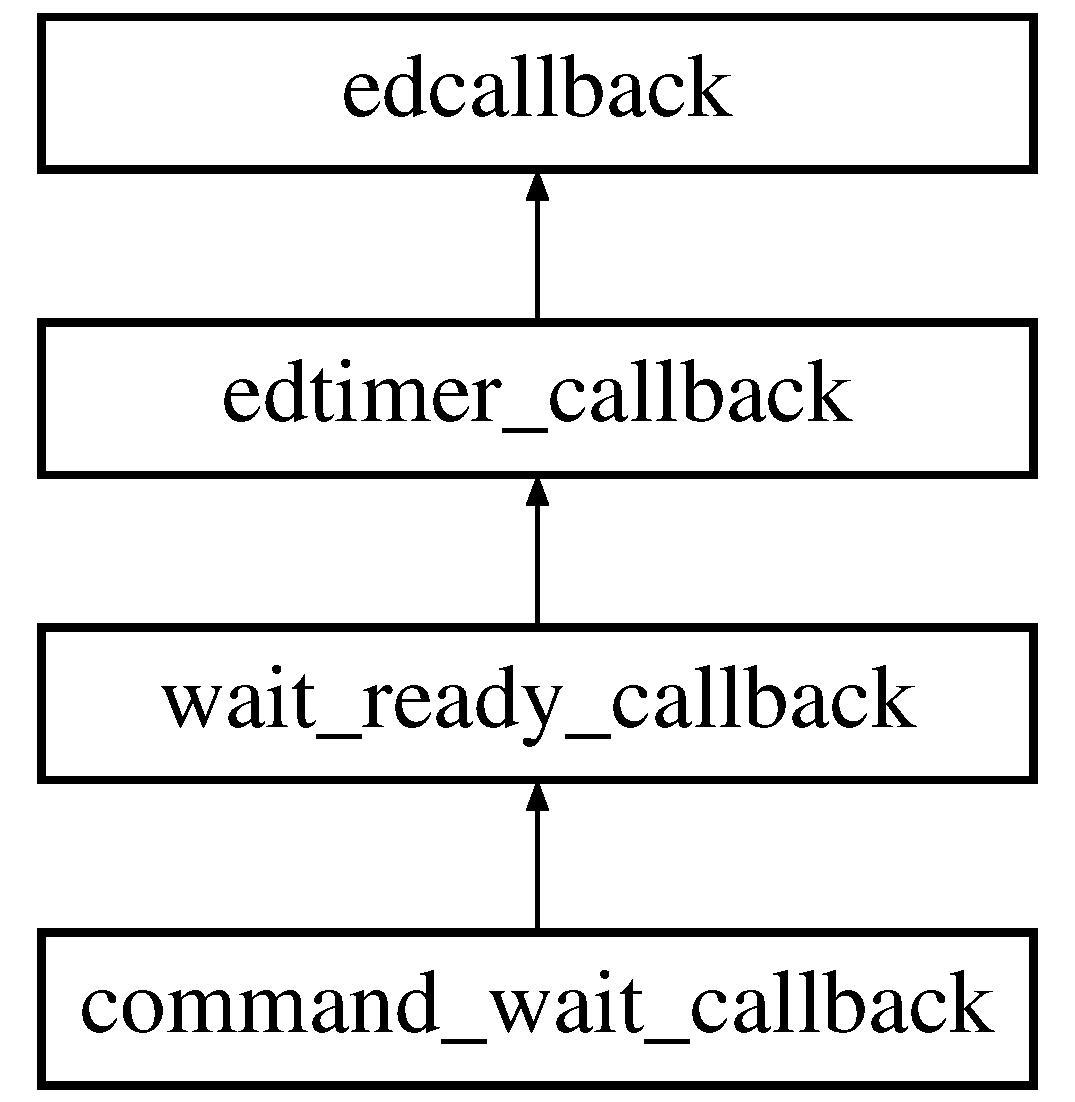
\includegraphics[height=4.000000cm]{structcommand__wait__callback}
\end{center}
\end{figure}
\subsection*{Public Member Functions}
\begin{DoxyCompactItemize}
\item 
\hyperlink{structcommand__wait__callback_ad7cfd5e02bb8af294a245b120bb542c7}{command\-\_\-wait\-\_\-callback} (\hyperlink{classedthreaded__fd}{edthreaded\-\_\-fd} $\ast$\-\_\-handle)
\item 
void \hyperlink{structcommand__wait__callback_ae5ab034230cd73f6203cee386ba1993c}{exec} ()
\end{DoxyCompactItemize}
\subsection*{Public Attributes}
\begin{DoxyCompactItemize}
\item 
\hyperlink{classedthreaded__fd}{edthreaded\-\_\-fd} $\ast$ \hyperlink{structcommand__wait__callback_a0abd24ce601b0e1452cde7eddb7b85b9}{handle}
\end{DoxyCompactItemize}


\subsection{Constructor \& Destructor Documentation}
\hypertarget{structcommand__wait__callback_ad7cfd5e02bb8af294a245b120bb542c7}{\index{command\-\_\-wait\-\_\-callback@{command\-\_\-wait\-\_\-callback}!command\-\_\-wait\-\_\-callback@{command\-\_\-wait\-\_\-callback}}
\index{command\-\_\-wait\-\_\-callback@{command\-\_\-wait\-\_\-callback}!command_wait_callback@{command\-\_\-wait\-\_\-callback}}
\subsubsection[{command\-\_\-wait\-\_\-callback}]{\setlength{\rightskip}{0pt plus 5cm}command\-\_\-wait\-\_\-callback\-::command\-\_\-wait\-\_\-callback (
\begin{DoxyParamCaption}
\item[{{\bf edthreaded\-\_\-fd} $\ast$}]{\-\_\-handle}
\end{DoxyParamCaption}
)\hspace{0.3cm}{\ttfamily [inline]}}}\label{structcommand__wait__callback_ad7cfd5e02bb8af294a245b120bb542c7}


\subsection{Member Function Documentation}
\hypertarget{structcommand__wait__callback_ae5ab034230cd73f6203cee386ba1993c}{\index{command\-\_\-wait\-\_\-callback@{command\-\_\-wait\-\_\-callback}!exec@{exec}}
\index{exec@{exec}!command_wait_callback@{command\-\_\-wait\-\_\-callback}}
\subsubsection[{exec}]{\setlength{\rightskip}{0pt plus 5cm}void command\-\_\-wait\-\_\-callback\-::exec (
\begin{DoxyParamCaption}
{}
\end{DoxyParamCaption}
)\hspace{0.3cm}{\ttfamily [inline]}, {\ttfamily [virtual]}}}\label{structcommand__wait__callback_ae5ab034230cd73f6203cee386ba1993c}


Reimplemented from \hyperlink{structwait__ready__callback_a305d57ffdd8bc5d3682dfa4a83431708}{wait\-\_\-ready\-\_\-callback}.



\subsection{Member Data Documentation}
\hypertarget{structcommand__wait__callback_a0abd24ce601b0e1452cde7eddb7b85b9}{\index{command\-\_\-wait\-\_\-callback@{command\-\_\-wait\-\_\-callback}!handle@{handle}}
\index{handle@{handle}!command_wait_callback@{command\-\_\-wait\-\_\-callback}}
\subsubsection[{handle}]{\setlength{\rightskip}{0pt plus 5cm}{\bf edthreaded\-\_\-fd}$\ast$ command\-\_\-wait\-\_\-callback\-::handle}}\label{structcommand__wait__callback_a0abd24ce601b0e1452cde7eddb7b85b9}


The documentation for this struct was generated from the following file\-:\begin{DoxyCompactItemize}
\item 
/home/dprandle/\-Documents/code/ctrlmod/include/\hyperlink{edthreaded__fd_8h}{edthreaded\-\_\-fd.\-h}\end{DoxyCompactItemize}

\hypertarget{structcomplete__scan__data__packet}{\section{complete\-\_\-scan\-\_\-data\-\_\-packet Struct Reference}
\label{structcomplete__scan__data__packet}\index{complete\-\_\-scan\-\_\-data\-\_\-packet@{complete\-\_\-scan\-\_\-data\-\_\-packet}}
}


{\ttfamily \#include $<$edrplidar\-\_\-packets.\-h$>$}

Inheritance diagram for complete\-\_\-scan\-\_\-data\-\_\-packet\-:\begin{figure}[H]
\begin{center}
\leavevmode
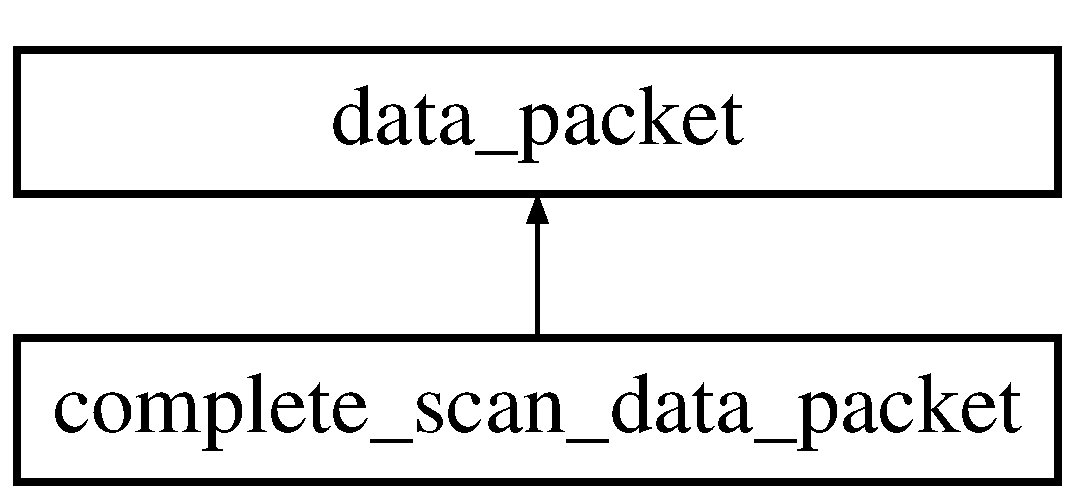
\includegraphics[height=2.000000cm]{structcomplete__scan__data__packet}
\end{center}
\end{figure}
\subsection*{Public Member Functions}
\begin{DoxyCompactItemize}
\item 
\hyperlink{structcomplete__scan__data__packet_a753b1906a3631b347472649120f748a4}{complete\-\_\-scan\-\_\-data\-\_\-packet} ()
\item 
virtual std\-::string \hyperlink{structcomplete__scan__data__packet_a35bfe3a588c176e844eea1c60453617e}{to\-String} ()
\item 
std\-::string \hyperlink{structcomplete__scan__data__packet_a144e017cea82952bda749de5692fdf6a}{type} ()
\item 
virtual uint32\-\_\-t \hyperlink{structcomplete__scan__data__packet_a2cc2871fdf24c03cd61f69acdec7cfb8}{size} ()
\item 
virtual uint8\-\_\-t \& \hyperlink{structcomplete__scan__data__packet_abcda1952cf162c478c0c0e1c77eaf34d}{operator\mbox{[}$\,$\mbox{]}} (uint32\-\_\-t index)
\item 
virtual uint8\-\_\-t $\ast$ \hyperlink{structcomplete__scan__data__packet_ad21ca3dc0a510662467edee56a02ae29}{dataptr} ()
\end{DoxyCompactItemize}
\subsection*{Static Public Member Functions}
\begin{DoxyCompactItemize}
\item 
static std\-::string \hyperlink{structcomplete__scan__data__packet_a1ecbf5f76b3b1f0b9938f8ab6ec7becf}{Type} ()
\item 
static uint32\-\_\-t \hyperlink{structcomplete__scan__data__packet_a45c7db37ae369581a70a6b2427489b22}{Size} ()
\end{DoxyCompactItemize}
\subsection*{Public Attributes}
\begin{DoxyCompactItemize}
\item 
\hyperlink{structscan__data__packet}{scan\-\_\-data\-\_\-packet} \hyperlink{structcomplete__scan__data__packet_ac0e845e17df7def88fee387aa81e681e}{data} \mbox{[}360\mbox{]}
\end{DoxyCompactItemize}


\subsection{Constructor \& Destructor Documentation}
\hypertarget{structcomplete__scan__data__packet_a753b1906a3631b347472649120f748a4}{\index{complete\-\_\-scan\-\_\-data\-\_\-packet@{complete\-\_\-scan\-\_\-data\-\_\-packet}!complete\-\_\-scan\-\_\-data\-\_\-packet@{complete\-\_\-scan\-\_\-data\-\_\-packet}}
\index{complete\-\_\-scan\-\_\-data\-\_\-packet@{complete\-\_\-scan\-\_\-data\-\_\-packet}!complete_scan_data_packet@{complete\-\_\-scan\-\_\-data\-\_\-packet}}
\subsubsection[{complete\-\_\-scan\-\_\-data\-\_\-packet}]{\setlength{\rightskip}{0pt plus 5cm}complete\-\_\-scan\-\_\-data\-\_\-packet\-::complete\-\_\-scan\-\_\-data\-\_\-packet (
\begin{DoxyParamCaption}
{}
\end{DoxyParamCaption}
)}}\label{structcomplete__scan__data__packet_a753b1906a3631b347472649120f748a4}


\subsection{Member Function Documentation}
\hypertarget{structcomplete__scan__data__packet_ad21ca3dc0a510662467edee56a02ae29}{\index{complete\-\_\-scan\-\_\-data\-\_\-packet@{complete\-\_\-scan\-\_\-data\-\_\-packet}!dataptr@{dataptr}}
\index{dataptr@{dataptr}!complete_scan_data_packet@{complete\-\_\-scan\-\_\-data\-\_\-packet}}
\subsubsection[{dataptr}]{\setlength{\rightskip}{0pt plus 5cm}virtual uint8\-\_\-t$\ast$ complete\-\_\-scan\-\_\-data\-\_\-packet\-::dataptr (
\begin{DoxyParamCaption}
{}
\end{DoxyParamCaption}
)\hspace{0.3cm}{\ttfamily [inline]}, {\ttfamily [virtual]}}}\label{structcomplete__scan__data__packet_ad21ca3dc0a510662467edee56a02ae29}


Implements \hyperlink{structdata__packet_ac53dcca572fc7cf7d71ae21d5c785365}{data\-\_\-packet}.

\hypertarget{structcomplete__scan__data__packet_abcda1952cf162c478c0c0e1c77eaf34d}{\index{complete\-\_\-scan\-\_\-data\-\_\-packet@{complete\-\_\-scan\-\_\-data\-\_\-packet}!operator\mbox{[}$\,$\mbox{]}@{operator[]}}
\index{operator\mbox{[}$\,$\mbox{]}@{operator[]}!complete_scan_data_packet@{complete\-\_\-scan\-\_\-data\-\_\-packet}}
\subsubsection[{operator[]}]{\setlength{\rightskip}{0pt plus 5cm}virtual uint8\-\_\-t\& complete\-\_\-scan\-\_\-data\-\_\-packet\-::operator\mbox{[}$\,$\mbox{]} (
\begin{DoxyParamCaption}
\item[{uint32\-\_\-t}]{index}
\end{DoxyParamCaption}
)\hspace{0.3cm}{\ttfamily [inline]}, {\ttfamily [virtual]}}}\label{structcomplete__scan__data__packet_abcda1952cf162c478c0c0e1c77eaf34d}


Implements \hyperlink{structdata__packet_a8f0d95d4a7a7089b45cef14e45b0c21b}{data\-\_\-packet}.

\hypertarget{structcomplete__scan__data__packet_a2cc2871fdf24c03cd61f69acdec7cfb8}{\index{complete\-\_\-scan\-\_\-data\-\_\-packet@{complete\-\_\-scan\-\_\-data\-\_\-packet}!size@{size}}
\index{size@{size}!complete_scan_data_packet@{complete\-\_\-scan\-\_\-data\-\_\-packet}}
\subsubsection[{size}]{\setlength{\rightskip}{0pt plus 5cm}virtual uint32\-\_\-t complete\-\_\-scan\-\_\-data\-\_\-packet\-::size (
\begin{DoxyParamCaption}
{}
\end{DoxyParamCaption}
)\hspace{0.3cm}{\ttfamily [inline]}, {\ttfamily [virtual]}}}\label{structcomplete__scan__data__packet_a2cc2871fdf24c03cd61f69acdec7cfb8}


Implements \hyperlink{structdata__packet_ab5c9259a79cde0dc60d75135fe8464f6}{data\-\_\-packet}.

\hypertarget{structcomplete__scan__data__packet_a45c7db37ae369581a70a6b2427489b22}{\index{complete\-\_\-scan\-\_\-data\-\_\-packet@{complete\-\_\-scan\-\_\-data\-\_\-packet}!Size@{Size}}
\index{Size@{Size}!complete_scan_data_packet@{complete\-\_\-scan\-\_\-data\-\_\-packet}}
\subsubsection[{Size}]{\setlength{\rightskip}{0pt plus 5cm}static uint32\-\_\-t complete\-\_\-scan\-\_\-data\-\_\-packet\-::\-Size (
\begin{DoxyParamCaption}
{}
\end{DoxyParamCaption}
)\hspace{0.3cm}{\ttfamily [inline]}, {\ttfamily [static]}}}\label{structcomplete__scan__data__packet_a45c7db37ae369581a70a6b2427489b22}
\hypertarget{structcomplete__scan__data__packet_a35bfe3a588c176e844eea1c60453617e}{\index{complete\-\_\-scan\-\_\-data\-\_\-packet@{complete\-\_\-scan\-\_\-data\-\_\-packet}!to\-String@{to\-String}}
\index{to\-String@{to\-String}!complete_scan_data_packet@{complete\-\_\-scan\-\_\-data\-\_\-packet}}
\subsubsection[{to\-String}]{\setlength{\rightskip}{0pt plus 5cm}std\-::string complete\-\_\-scan\-\_\-data\-\_\-packet\-::to\-String (
\begin{DoxyParamCaption}
{}
\end{DoxyParamCaption}
)\hspace{0.3cm}{\ttfamily [virtual]}}}\label{structcomplete__scan__data__packet_a35bfe3a588c176e844eea1c60453617e}


Implements \hyperlink{structdata__packet_ad7ce179caef76c895bfc778862bc15ac}{data\-\_\-packet}.

\hypertarget{structcomplete__scan__data__packet_a144e017cea82952bda749de5692fdf6a}{\index{complete\-\_\-scan\-\_\-data\-\_\-packet@{complete\-\_\-scan\-\_\-data\-\_\-packet}!type@{type}}
\index{type@{type}!complete_scan_data_packet@{complete\-\_\-scan\-\_\-data\-\_\-packet}}
\subsubsection[{type}]{\setlength{\rightskip}{0pt plus 5cm}std\-::string complete\-\_\-scan\-\_\-data\-\_\-packet\-::type (
\begin{DoxyParamCaption}
{}
\end{DoxyParamCaption}
)\hspace{0.3cm}{\ttfamily [inline]}, {\ttfamily [virtual]}}}\label{structcomplete__scan__data__packet_a144e017cea82952bda749de5692fdf6a}


Implements \hyperlink{structdata__packet_af0795581f2d57a8c14a88009da37aee1}{data\-\_\-packet}.

\hypertarget{structcomplete__scan__data__packet_a1ecbf5f76b3b1f0b9938f8ab6ec7becf}{\index{complete\-\_\-scan\-\_\-data\-\_\-packet@{complete\-\_\-scan\-\_\-data\-\_\-packet}!Type@{Type}}
\index{Type@{Type}!complete_scan_data_packet@{complete\-\_\-scan\-\_\-data\-\_\-packet}}
\subsubsection[{Type}]{\setlength{\rightskip}{0pt plus 5cm}static std\-::string complete\-\_\-scan\-\_\-data\-\_\-packet\-::\-Type (
\begin{DoxyParamCaption}
{}
\end{DoxyParamCaption}
)\hspace{0.3cm}{\ttfamily [inline]}, {\ttfamily [static]}}}\label{structcomplete__scan__data__packet_a1ecbf5f76b3b1f0b9938f8ab6ec7becf}


\subsection{Member Data Documentation}
\hypertarget{structcomplete__scan__data__packet_ac0e845e17df7def88fee387aa81e681e}{\index{complete\-\_\-scan\-\_\-data\-\_\-packet@{complete\-\_\-scan\-\_\-data\-\_\-packet}!data@{data}}
\index{data@{data}!complete_scan_data_packet@{complete\-\_\-scan\-\_\-data\-\_\-packet}}
\subsubsection[{data}]{\setlength{\rightskip}{0pt plus 5cm}{\bf scan\-\_\-data\-\_\-packet} complete\-\_\-scan\-\_\-data\-\_\-packet\-::data\mbox{[}360\mbox{]}}}\label{structcomplete__scan__data__packet_ac0e845e17df7def88fee387aa81e681e}


The documentation for this struct was generated from the following files\-:\begin{DoxyCompactItemize}
\item 
/home/dprandle/\-Documents/code/ctrlmod/include/\hyperlink{edrplidar__packets_8h}{edrplidar\-\_\-packets.\-h}\item 
/home/dprandle/\-Documents/code/ctrlmod/src/\hyperlink{edrplidar__packets_8cpp}{edrplidar\-\_\-packets.\-cpp}\end{DoxyCompactItemize}

\hypertarget{structdata__packet}{\section{data\-\_\-packet Struct Reference}
\label{structdata__packet}\index{data\-\_\-packet@{data\-\_\-packet}}
}


{\ttfamily \#include $<$edrplidar\-\_\-packets.\-h$>$}

Inheritance diagram for data\-\_\-packet\-:\begin{figure}[H]
\begin{center}
\leavevmode
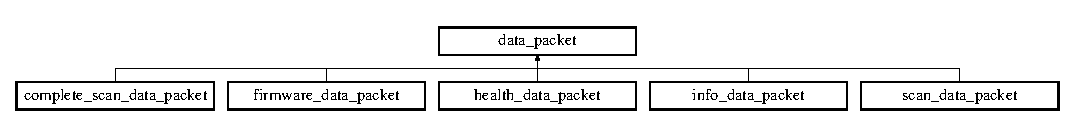
\includegraphics[height=1.251397cm]{structdata__packet}
\end{center}
\end{figure}
\subsection*{Public Member Functions}
\begin{DoxyCompactItemize}
\item 
\hyperlink{structdata__packet_aeac45f0ad8cb14657bd37306170b2afd}{data\-\_\-packet} ()
\item 
virtual \hyperlink{structdata__packet_a63fd3fc8f94d6bd4fb3accfe612cfe3b}{$\sim$data\-\_\-packet} ()
\item 
virtual std\-::string \hyperlink{structdata__packet_ad7ce179caef76c895bfc778862bc15ac}{to\-String} ()=0
\item 
virtual std\-::string \hyperlink{structdata__packet_af0795581f2d57a8c14a88009da37aee1}{type} ()=0
\item 
virtual uint32\-\_\-t \hyperlink{structdata__packet_ab5c9259a79cde0dc60d75135fe8464f6}{size} ()=0
\item 
virtual uint8\-\_\-t \& \hyperlink{structdata__packet_a8f0d95d4a7a7089b45cef14e45b0c21b}{operator\mbox{[}$\,$\mbox{]}} (uint32\-\_\-t index)=0
\item 
virtual uint8\-\_\-t $\ast$ \hyperlink{structdata__packet_ac53dcca572fc7cf7d71ae21d5c785365}{dataptr} ()=0
\end{DoxyCompactItemize}


\subsection{Constructor \& Destructor Documentation}
\hypertarget{structdata__packet_aeac45f0ad8cb14657bd37306170b2afd}{\index{data\-\_\-packet@{data\-\_\-packet}!data\-\_\-packet@{data\-\_\-packet}}
\index{data\-\_\-packet@{data\-\_\-packet}!data_packet@{data\-\_\-packet}}
\subsubsection[{data\-\_\-packet}]{\setlength{\rightskip}{0pt plus 5cm}data\-\_\-packet\-::data\-\_\-packet (
\begin{DoxyParamCaption}
{}
\end{DoxyParamCaption}
)\hspace{0.3cm}{\ttfamily [inline]}}}\label{structdata__packet_aeac45f0ad8cb14657bd37306170b2afd}
\hypertarget{structdata__packet_a63fd3fc8f94d6bd4fb3accfe612cfe3b}{\index{data\-\_\-packet@{data\-\_\-packet}!$\sim$data\-\_\-packet@{$\sim$data\-\_\-packet}}
\index{$\sim$data\-\_\-packet@{$\sim$data\-\_\-packet}!data_packet@{data\-\_\-packet}}
\subsubsection[{$\sim$data\-\_\-packet}]{\setlength{\rightskip}{0pt plus 5cm}virtual data\-\_\-packet\-::$\sim$data\-\_\-packet (
\begin{DoxyParamCaption}
{}
\end{DoxyParamCaption}
)\hspace{0.3cm}{\ttfamily [inline]}, {\ttfamily [virtual]}}}\label{structdata__packet_a63fd3fc8f94d6bd4fb3accfe612cfe3b}


\subsection{Member Function Documentation}
\hypertarget{structdata__packet_ac53dcca572fc7cf7d71ae21d5c785365}{\index{data\-\_\-packet@{data\-\_\-packet}!dataptr@{dataptr}}
\index{dataptr@{dataptr}!data_packet@{data\-\_\-packet}}
\subsubsection[{dataptr}]{\setlength{\rightskip}{0pt plus 5cm}virtual uint8\-\_\-t$\ast$ data\-\_\-packet\-::dataptr (
\begin{DoxyParamCaption}
{}
\end{DoxyParamCaption}
)\hspace{0.3cm}{\ttfamily [pure virtual]}}}\label{structdata__packet_ac53dcca572fc7cf7d71ae21d5c785365}


Implemented in \hyperlink{structfirmware__data__packet_ab080f05c847592a2578ee307d5af31fc}{firmware\-\_\-data\-\_\-packet}, \hyperlink{structinfo__data__packet_a2b730e457ee372ad1d40d4bbc22928cc}{info\-\_\-data\-\_\-packet}, \hyperlink{structhealth__data__packet_a8378ecf34528f77f6d50937c3ad02c8d}{health\-\_\-data\-\_\-packet}, \hyperlink{structcomplete__scan__data__packet_ad21ca3dc0a510662467edee56a02ae29}{complete\-\_\-scan\-\_\-data\-\_\-packet}, and \hyperlink{structscan__data__packet_a376edae10eddfa50b3684e801a0a8f3a}{scan\-\_\-data\-\_\-packet}.

\hypertarget{structdata__packet_a8f0d95d4a7a7089b45cef14e45b0c21b}{\index{data\-\_\-packet@{data\-\_\-packet}!operator\mbox{[}$\,$\mbox{]}@{operator[]}}
\index{operator\mbox{[}$\,$\mbox{]}@{operator[]}!data_packet@{data\-\_\-packet}}
\subsubsection[{operator[]}]{\setlength{\rightskip}{0pt plus 5cm}virtual uint8\-\_\-t\& data\-\_\-packet\-::operator\mbox{[}$\,$\mbox{]} (
\begin{DoxyParamCaption}
\item[{uint32\-\_\-t}]{index}
\end{DoxyParamCaption}
)\hspace{0.3cm}{\ttfamily [pure virtual]}}}\label{structdata__packet_a8f0d95d4a7a7089b45cef14e45b0c21b}


Implemented in \hyperlink{structfirmware__data__packet_a16d28be180847cb45fc4dbf0417756b9}{firmware\-\_\-data\-\_\-packet}, \hyperlink{structinfo__data__packet_a5a78a794ee110ed9bb4a4bb97d57f9f3}{info\-\_\-data\-\_\-packet}, \hyperlink{structhealth__data__packet_aa96359c2b7100e17905e02c7ab68ca59}{health\-\_\-data\-\_\-packet}, \hyperlink{structcomplete__scan__data__packet_abcda1952cf162c478c0c0e1c77eaf34d}{complete\-\_\-scan\-\_\-data\-\_\-packet}, and \hyperlink{structscan__data__packet_ac8b9b314239dd2663a7d2b98e5cd1c1a}{scan\-\_\-data\-\_\-packet}.

\hypertarget{structdata__packet_ab5c9259a79cde0dc60d75135fe8464f6}{\index{data\-\_\-packet@{data\-\_\-packet}!size@{size}}
\index{size@{size}!data_packet@{data\-\_\-packet}}
\subsubsection[{size}]{\setlength{\rightskip}{0pt plus 5cm}virtual uint32\-\_\-t data\-\_\-packet\-::size (
\begin{DoxyParamCaption}
{}
\end{DoxyParamCaption}
)\hspace{0.3cm}{\ttfamily [pure virtual]}}}\label{structdata__packet_ab5c9259a79cde0dc60d75135fe8464f6}


Implemented in \hyperlink{structfirmware__data__packet_a3231148228aee555265b90ab30fea9ec}{firmware\-\_\-data\-\_\-packet}, \hyperlink{structinfo__data__packet_a8852d00d040d27ba824dc333a8f66f44}{info\-\_\-data\-\_\-packet}, \hyperlink{structhealth__data__packet_a85329a68f718099b6cefcf65fab75077}{health\-\_\-data\-\_\-packet}, \hyperlink{structcomplete__scan__data__packet_a2cc2871fdf24c03cd61f69acdec7cfb8}{complete\-\_\-scan\-\_\-data\-\_\-packet}, and \hyperlink{structscan__data__packet_a2678e9313e25c529abba1c1ba5ff3cba}{scan\-\_\-data\-\_\-packet}.

\hypertarget{structdata__packet_ad7ce179caef76c895bfc778862bc15ac}{\index{data\-\_\-packet@{data\-\_\-packet}!to\-String@{to\-String}}
\index{to\-String@{to\-String}!data_packet@{data\-\_\-packet}}
\subsubsection[{to\-String}]{\setlength{\rightskip}{0pt plus 5cm}virtual std\-::string data\-\_\-packet\-::to\-String (
\begin{DoxyParamCaption}
{}
\end{DoxyParamCaption}
)\hspace{0.3cm}{\ttfamily [pure virtual]}}}\label{structdata__packet_ad7ce179caef76c895bfc778862bc15ac}


Implemented in \hyperlink{structfirmware__data__packet_a1ff72c5345b4325fd955bb20c9860d89}{firmware\-\_\-data\-\_\-packet}, \hyperlink{structinfo__data__packet_a8c8b12d30a12b931740eb9c4cdc84315}{info\-\_\-data\-\_\-packet}, \hyperlink{structhealth__data__packet_a89e96e87bdcf2ecc52260a9d98e37995}{health\-\_\-data\-\_\-packet}, \hyperlink{structcomplete__scan__data__packet_a35bfe3a588c176e844eea1c60453617e}{complete\-\_\-scan\-\_\-data\-\_\-packet}, and \hyperlink{structscan__data__packet_aa8d4b795a798f413149c93760de6577f}{scan\-\_\-data\-\_\-packet}.

\hypertarget{structdata__packet_af0795581f2d57a8c14a88009da37aee1}{\index{data\-\_\-packet@{data\-\_\-packet}!type@{type}}
\index{type@{type}!data_packet@{data\-\_\-packet}}
\subsubsection[{type}]{\setlength{\rightskip}{0pt plus 5cm}virtual std\-::string data\-\_\-packet\-::type (
\begin{DoxyParamCaption}
{}
\end{DoxyParamCaption}
)\hspace{0.3cm}{\ttfamily [pure virtual]}}}\label{structdata__packet_af0795581f2d57a8c14a88009da37aee1}


Implemented in \hyperlink{structfirmware__data__packet_a84cd6f60b9d5ef46ab5c4695d6de3d48}{firmware\-\_\-data\-\_\-packet}, \hyperlink{structinfo__data__packet_a85dfeae92d487d55b6d57e95e0c2b662}{info\-\_\-data\-\_\-packet}, \hyperlink{structhealth__data__packet_abc386acf1fcf42086f1fc791d2718dff}{health\-\_\-data\-\_\-packet}, \hyperlink{structcomplete__scan__data__packet_a144e017cea82952bda749de5692fdf6a}{complete\-\_\-scan\-\_\-data\-\_\-packet}, and \hyperlink{structscan__data__packet_a8401263b8927ca5a67ca23c8797cc67e}{scan\-\_\-data\-\_\-packet}.



The documentation for this struct was generated from the following file\-:\begin{DoxyCompactItemize}
\item 
/home/dprandle/\-Documents/code/ctrlmod/include/\hyperlink{edrplidar__packets_8h}{edrplidar\-\_\-packets.\-h}\end{DoxyCompactItemize}

\hypertarget{structeduart_1_1DataFormat}{\section{eduart\-:\-:Data\-Format Struct Reference}
\label{structeduart_1_1DataFormat}\index{eduart\-::\-Data\-Format@{eduart\-::\-Data\-Format}}
}


{\ttfamily \#include $<$eduart.\-h$>$}

\subsection*{Public Member Functions}
\begin{DoxyCompactItemize}
\item 
\hyperlink{structeduart_1_1DataFormat_a25d5d11b4a91ae142838d6d88b96a5b3}{Data\-Format} ()
\end{DoxyCompactItemize}
\subsection*{Public Attributes}
\begin{DoxyCompactItemize}
\item 
\hyperlink{classeduart_a5211d2ecc2f21296eafe114ca999abb2}{Data\-Bits} \hyperlink{structeduart_1_1DataFormat_a9bcbfb5d9a0e9720440b7487e300725a}{db}
\item 
\hyperlink{classeduart_ab706a92a2abdd39b748492f26d89fa75}{Parity} \hyperlink{structeduart_1_1DataFormat_acb10f62257fad3e05c072b0926d04697}{p}
\item 
\hyperlink{classeduart_a81d64a65349ee87e6bff9e99c1a2a4fa}{Stop\-Bits} \hyperlink{structeduart_1_1DataFormat_a00afa036bb12c742f13548afa4fb593e}{sb}
\end{DoxyCompactItemize}


\subsection{Constructor \& Destructor Documentation}
\hypertarget{structeduart_1_1DataFormat_a25d5d11b4a91ae142838d6d88b96a5b3}{\index{eduart\-::\-Data\-Format@{eduart\-::\-Data\-Format}!Data\-Format@{Data\-Format}}
\index{Data\-Format@{Data\-Format}!eduart::DataFormat@{eduart\-::\-Data\-Format}}
\subsubsection[{Data\-Format}]{\setlength{\rightskip}{0pt plus 5cm}eduart\-::\-Data\-Format\-::\-Data\-Format (
\begin{DoxyParamCaption}
{}
\end{DoxyParamCaption}
)\hspace{0.3cm}{\ttfamily [inline]}}}\label{structeduart_1_1DataFormat_a25d5d11b4a91ae142838d6d88b96a5b3}


\subsection{Member Data Documentation}
\hypertarget{structeduart_1_1DataFormat_a9bcbfb5d9a0e9720440b7487e300725a}{\index{eduart\-::\-Data\-Format@{eduart\-::\-Data\-Format}!db@{db}}
\index{db@{db}!eduart::DataFormat@{eduart\-::\-Data\-Format}}
\subsubsection[{db}]{\setlength{\rightskip}{0pt plus 5cm}{\bf Data\-Bits} eduart\-::\-Data\-Format\-::db}}\label{structeduart_1_1DataFormat_a9bcbfb5d9a0e9720440b7487e300725a}
\hypertarget{structeduart_1_1DataFormat_acb10f62257fad3e05c072b0926d04697}{\index{eduart\-::\-Data\-Format@{eduart\-::\-Data\-Format}!p@{p}}
\index{p@{p}!eduart::DataFormat@{eduart\-::\-Data\-Format}}
\subsubsection[{p}]{\setlength{\rightskip}{0pt plus 5cm}{\bf Parity} eduart\-::\-Data\-Format\-::p}}\label{structeduart_1_1DataFormat_acb10f62257fad3e05c072b0926d04697}
\hypertarget{structeduart_1_1DataFormat_a00afa036bb12c742f13548afa4fb593e}{\index{eduart\-::\-Data\-Format@{eduart\-::\-Data\-Format}!sb@{sb}}
\index{sb@{sb}!eduart::DataFormat@{eduart\-::\-Data\-Format}}
\subsubsection[{sb}]{\setlength{\rightskip}{0pt plus 5cm}{\bf Stop\-Bits} eduart\-::\-Data\-Format\-::sb}}\label{structeduart_1_1DataFormat_a00afa036bb12c742f13548afa4fb593e}


The documentation for this struct was generated from the following file\-:\begin{DoxyCompactItemize}
\item 
/home/dprandle/\-Documents/code/ctrlmod/include/\hyperlink{eduart_8h}{eduart.\-h}\end{DoxyCompactItemize}

\hypertarget{structdescriptor__packet}{\section{descriptor\-\_\-packet Struct Reference}
\label{structdescriptor__packet}\index{descriptor\-\_\-packet@{descriptor\-\_\-packet}}
}


{\ttfamily \#include $<$edrplidar\-\_\-packets.\-h$>$}

Inheritance diagram for descriptor\-\_\-packet\-:\begin{figure}[H]
\begin{center}
\leavevmode
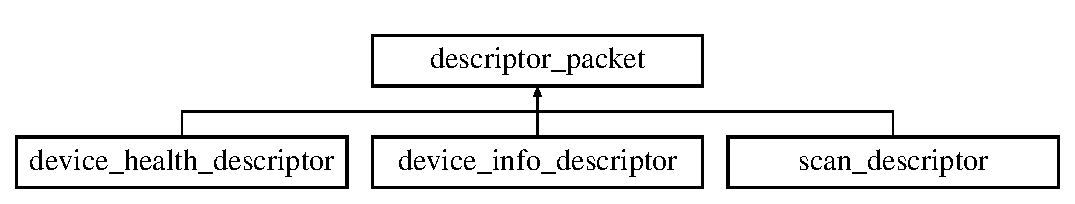
\includegraphics[height=2.000000cm]{structdescriptor__packet}
\end{center}
\end{figure}
\subsection*{Public Member Functions}
\begin{DoxyCompactItemize}
\item 
\hyperlink{structdescriptor__packet_acb50c5d7e23d6b85a2310672d9f17e95}{descriptor\-\_\-packet} (uint8\-\_\-t drlen0\-\_\-=0x00, uint8\-\_\-t drlen1\-\_\-=0x00, uint8\-\_\-t drlen2\-\_\-=0x00, uint8\-\_\-t drlen3\-\_\-smode\-\_\-=0x00, uint8\-\_\-t datatype\-\_\-=0x00)
\item 
virtual \hyperlink{structdescriptor__packet_acd7f79e7aefbdf4f6b0638ab75df6d46}{$\sim$descriptor\-\_\-packet} ()
\item 
virtual std\-::string \hyperlink{structdescriptor__packet_ad08369aae987f91544cee5e8f2267f2f}{type} ()=0
\item 
uint32\-\_\-t \hyperlink{structdescriptor__packet_a3b14c4024796ba8b45f582b0bd7d1f50}{size} ()
\item 
uint8\-\_\-t \& \hyperlink{structdescriptor__packet_a92b50972015f1bb1b4a99d0f0910c3e3}{operator\mbox{[}$\,$\mbox{]}} (uint32\-\_\-t index)
\end{DoxyCompactItemize}
\subsection*{Static Public Member Functions}
\begin{DoxyCompactItemize}
\item 
static uint32\-\_\-t \hyperlink{structdescriptor__packet_ab197e4207edc6c708dca8d0b0bbfc098}{Size} ()
\end{DoxyCompactItemize}
\subsection*{Public Attributes}
\begin{DoxyCompactItemize}
\item 
\begin{tabbing}
xx\=xx\=xx\=xx\=xx\=xx\=xx\=xx\=xx\=\kill
union \{\\
\>struct \{\\
\>\>uint8\_t \hyperlink{structdescriptor__packet_a3187e2d5d736ad8ad2e5bfa39832851e}{s1}\\
\>\>uint8\_t \hyperlink{structdescriptor__packet_aecf654bc09c8021678564ef2938e9190}{s2}\\
\>\>uint8\_t \hyperlink{structdescriptor__packet_afaa19b5c2d3324b188e5f1b24a07c3fb}{drlen0}\\
\>\>uint8\_t \hyperlink{structdescriptor__packet_a3f182b48556355988a8f983fb9dc434b}{drlen1}\\
\>\>uint8\_t \hyperlink{structdescriptor__packet_ab3437c0152e4a97a832ce80da0075da6}{drlen2}\\
\>\>uint8\_t \hyperlink{structdescriptor__packet_afc7b12b3c81172ec5ebf5fe28413dcfd}{drlen3\_smode}\\
\>\>uint8\_t \hyperlink{structdescriptor__packet_ad1bea15d0f3741d718d82689884c787d}{datatype}\\
\>\} \\
\>uint8\_t \hyperlink{structdescriptor__packet_ad0ac7e3aa5ab78a411f748ae0baed2f3}{data} \mbox{[}7\mbox{]}\\
\}; \\

\end{tabbing}\end{DoxyCompactItemize}


\subsection{Constructor \& Destructor Documentation}
\hypertarget{structdescriptor__packet_acb50c5d7e23d6b85a2310672d9f17e95}{\index{descriptor\-\_\-packet@{descriptor\-\_\-packet}!descriptor\-\_\-packet@{descriptor\-\_\-packet}}
\index{descriptor\-\_\-packet@{descriptor\-\_\-packet}!descriptor_packet@{descriptor\-\_\-packet}}
\subsubsection[{descriptor\-\_\-packet}]{\setlength{\rightskip}{0pt plus 5cm}descriptor\-\_\-packet\-::descriptor\-\_\-packet (
\begin{DoxyParamCaption}
\item[{uint8\-\_\-t}]{drlen0\-\_\- = {\ttfamily 0x00}, }
\item[{uint8\-\_\-t}]{drlen1\-\_\- = {\ttfamily 0x00}, }
\item[{uint8\-\_\-t}]{drlen2\-\_\- = {\ttfamily 0x00}, }
\item[{uint8\-\_\-t}]{drlen3\-\_\-smode\-\_\- = {\ttfamily 0x00}, }
\item[{uint8\-\_\-t}]{datatype\-\_\- = {\ttfamily 0x00}}
\end{DoxyParamCaption}
)\hspace{0.3cm}{\ttfamily [inline]}}}\label{structdescriptor__packet_acb50c5d7e23d6b85a2310672d9f17e95}
\hypertarget{structdescriptor__packet_acd7f79e7aefbdf4f6b0638ab75df6d46}{\index{descriptor\-\_\-packet@{descriptor\-\_\-packet}!$\sim$descriptor\-\_\-packet@{$\sim$descriptor\-\_\-packet}}
\index{$\sim$descriptor\-\_\-packet@{$\sim$descriptor\-\_\-packet}!descriptor_packet@{descriptor\-\_\-packet}}
\subsubsection[{$\sim$descriptor\-\_\-packet}]{\setlength{\rightskip}{0pt plus 5cm}virtual descriptor\-\_\-packet\-::$\sim$descriptor\-\_\-packet (
\begin{DoxyParamCaption}
{}
\end{DoxyParamCaption}
)\hspace{0.3cm}{\ttfamily [inline]}, {\ttfamily [virtual]}}}\label{structdescriptor__packet_acd7f79e7aefbdf4f6b0638ab75df6d46}


\subsection{Member Function Documentation}
\hypertarget{structdescriptor__packet_a92b50972015f1bb1b4a99d0f0910c3e3}{\index{descriptor\-\_\-packet@{descriptor\-\_\-packet}!operator\mbox{[}$\,$\mbox{]}@{operator[]}}
\index{operator\mbox{[}$\,$\mbox{]}@{operator[]}!descriptor_packet@{descriptor\-\_\-packet}}
\subsubsection[{operator[]}]{\setlength{\rightskip}{0pt plus 5cm}uint8\-\_\-t\& descriptor\-\_\-packet\-::operator\mbox{[}$\,$\mbox{]} (
\begin{DoxyParamCaption}
\item[{uint32\-\_\-t}]{index}
\end{DoxyParamCaption}
)\hspace{0.3cm}{\ttfamily [inline]}}}\label{structdescriptor__packet_a92b50972015f1bb1b4a99d0f0910c3e3}
\hypertarget{structdescriptor__packet_a3b14c4024796ba8b45f582b0bd7d1f50}{\index{descriptor\-\_\-packet@{descriptor\-\_\-packet}!size@{size}}
\index{size@{size}!descriptor_packet@{descriptor\-\_\-packet}}
\subsubsection[{size}]{\setlength{\rightskip}{0pt plus 5cm}uint32\-\_\-t descriptor\-\_\-packet\-::size (
\begin{DoxyParamCaption}
{}
\end{DoxyParamCaption}
)\hspace{0.3cm}{\ttfamily [inline]}}}\label{structdescriptor__packet_a3b14c4024796ba8b45f582b0bd7d1f50}
\hypertarget{structdescriptor__packet_ab197e4207edc6c708dca8d0b0bbfc098}{\index{descriptor\-\_\-packet@{descriptor\-\_\-packet}!Size@{Size}}
\index{Size@{Size}!descriptor_packet@{descriptor\-\_\-packet}}
\subsubsection[{Size}]{\setlength{\rightskip}{0pt plus 5cm}static uint32\-\_\-t descriptor\-\_\-packet\-::\-Size (
\begin{DoxyParamCaption}
{}
\end{DoxyParamCaption}
)\hspace{0.3cm}{\ttfamily [inline]}, {\ttfamily [static]}}}\label{structdescriptor__packet_ab197e4207edc6c708dca8d0b0bbfc098}
\hypertarget{structdescriptor__packet_ad08369aae987f91544cee5e8f2267f2f}{\index{descriptor\-\_\-packet@{descriptor\-\_\-packet}!type@{type}}
\index{type@{type}!descriptor_packet@{descriptor\-\_\-packet}}
\subsubsection[{type}]{\setlength{\rightskip}{0pt plus 5cm}virtual std\-::string descriptor\-\_\-packet\-::type (
\begin{DoxyParamCaption}
{}
\end{DoxyParamCaption}
)\hspace{0.3cm}{\ttfamily [pure virtual]}}}\label{structdescriptor__packet_ad08369aae987f91544cee5e8f2267f2f}


Implemented in \hyperlink{structdevice__health__descriptor_a54b8725863d9ca6c640a8eb5e557109f}{device\-\_\-health\-\_\-descriptor}, \hyperlink{structdevice__info__descriptor_a52fb00aa7ddd64fb130622f1cae6f4e2}{device\-\_\-info\-\_\-descriptor}, and \hyperlink{structscan__descriptor_a3020edbf9b9ff7e8c50a150050e0ec6f}{scan\-\_\-descriptor}.



\subsection{Member Data Documentation}
\hypertarget{structdescriptor__packet_a9d52a25c1b5dbc1aa92301cfbb10db97}{\subsubsection[{"@33}]{\setlength{\rightskip}{0pt plus 5cm}union \{ ... \} }}\label{structdescriptor__packet_a9d52a25c1b5dbc1aa92301cfbb10db97}
\hypertarget{structdescriptor__packet_ad0ac7e3aa5ab78a411f748ae0baed2f3}{\index{descriptor\-\_\-packet@{descriptor\-\_\-packet}!data@{data}}
\index{data@{data}!descriptor_packet@{descriptor\-\_\-packet}}
\subsubsection[{data}]{\setlength{\rightskip}{0pt plus 5cm}uint8\-\_\-t descriptor\-\_\-packet\-::data\mbox{[}7\mbox{]}}}\label{structdescriptor__packet_ad0ac7e3aa5ab78a411f748ae0baed2f3}
\hypertarget{structdescriptor__packet_ad1bea15d0f3741d718d82689884c787d}{\index{descriptor\-\_\-packet@{descriptor\-\_\-packet}!datatype@{datatype}}
\index{datatype@{datatype}!descriptor_packet@{descriptor\-\_\-packet}}
\subsubsection[{datatype}]{\setlength{\rightskip}{0pt plus 5cm}uint8\-\_\-t descriptor\-\_\-packet\-::datatype}}\label{structdescriptor__packet_ad1bea15d0f3741d718d82689884c787d}
\hypertarget{structdescriptor__packet_afaa19b5c2d3324b188e5f1b24a07c3fb}{\index{descriptor\-\_\-packet@{descriptor\-\_\-packet}!drlen0@{drlen0}}
\index{drlen0@{drlen0}!descriptor_packet@{descriptor\-\_\-packet}}
\subsubsection[{drlen0}]{\setlength{\rightskip}{0pt plus 5cm}uint8\-\_\-t descriptor\-\_\-packet\-::drlen0}}\label{structdescriptor__packet_afaa19b5c2d3324b188e5f1b24a07c3fb}
\hypertarget{structdescriptor__packet_a3f182b48556355988a8f983fb9dc434b}{\index{descriptor\-\_\-packet@{descriptor\-\_\-packet}!drlen1@{drlen1}}
\index{drlen1@{drlen1}!descriptor_packet@{descriptor\-\_\-packet}}
\subsubsection[{drlen1}]{\setlength{\rightskip}{0pt plus 5cm}uint8\-\_\-t descriptor\-\_\-packet\-::drlen1}}\label{structdescriptor__packet_a3f182b48556355988a8f983fb9dc434b}
\hypertarget{structdescriptor__packet_ab3437c0152e4a97a832ce80da0075da6}{\index{descriptor\-\_\-packet@{descriptor\-\_\-packet}!drlen2@{drlen2}}
\index{drlen2@{drlen2}!descriptor_packet@{descriptor\-\_\-packet}}
\subsubsection[{drlen2}]{\setlength{\rightskip}{0pt plus 5cm}uint8\-\_\-t descriptor\-\_\-packet\-::drlen2}}\label{structdescriptor__packet_ab3437c0152e4a97a832ce80da0075da6}
\hypertarget{structdescriptor__packet_afc7b12b3c81172ec5ebf5fe28413dcfd}{\index{descriptor\-\_\-packet@{descriptor\-\_\-packet}!drlen3\-\_\-smode@{drlen3\-\_\-smode}}
\index{drlen3\-\_\-smode@{drlen3\-\_\-smode}!descriptor_packet@{descriptor\-\_\-packet}}
\subsubsection[{drlen3\-\_\-smode}]{\setlength{\rightskip}{0pt plus 5cm}uint8\-\_\-t descriptor\-\_\-packet\-::drlen3\-\_\-smode}}\label{structdescriptor__packet_afc7b12b3c81172ec5ebf5fe28413dcfd}
\hypertarget{structdescriptor__packet_a3187e2d5d736ad8ad2e5bfa39832851e}{\index{descriptor\-\_\-packet@{descriptor\-\_\-packet}!s1@{s1}}
\index{s1@{s1}!descriptor_packet@{descriptor\-\_\-packet}}
\subsubsection[{s1}]{\setlength{\rightskip}{0pt plus 5cm}uint8\-\_\-t descriptor\-\_\-packet\-::s1}}\label{structdescriptor__packet_a3187e2d5d736ad8ad2e5bfa39832851e}
\hypertarget{structdescriptor__packet_aecf654bc09c8021678564ef2938e9190}{\index{descriptor\-\_\-packet@{descriptor\-\_\-packet}!s2@{s2}}
\index{s2@{s2}!descriptor_packet@{descriptor\-\_\-packet}}
\subsubsection[{s2}]{\setlength{\rightskip}{0pt plus 5cm}uint8\-\_\-t descriptor\-\_\-packet\-::s2}}\label{structdescriptor__packet_aecf654bc09c8021678564ef2938e9190}


The documentation for this struct was generated from the following file\-:\begin{DoxyCompactItemize}
\item 
/home/dprandle/\-Documents/code/ctrlmod/include/\hyperlink{edrplidar__packets_8h}{edrplidar\-\_\-packets.\-h}\end{DoxyCompactItemize}

\hypertarget{structdevice__health__descriptor}{\section{device\-\_\-health\-\_\-descriptor Struct Reference}
\label{structdevice__health__descriptor}\index{device\-\_\-health\-\_\-descriptor@{device\-\_\-health\-\_\-descriptor}}
}


{\ttfamily \#include $<$edrplidar\-\_\-packets.\-h$>$}

Inheritance diagram for device\-\_\-health\-\_\-descriptor\-:\begin{figure}[H]
\begin{center}
\leavevmode
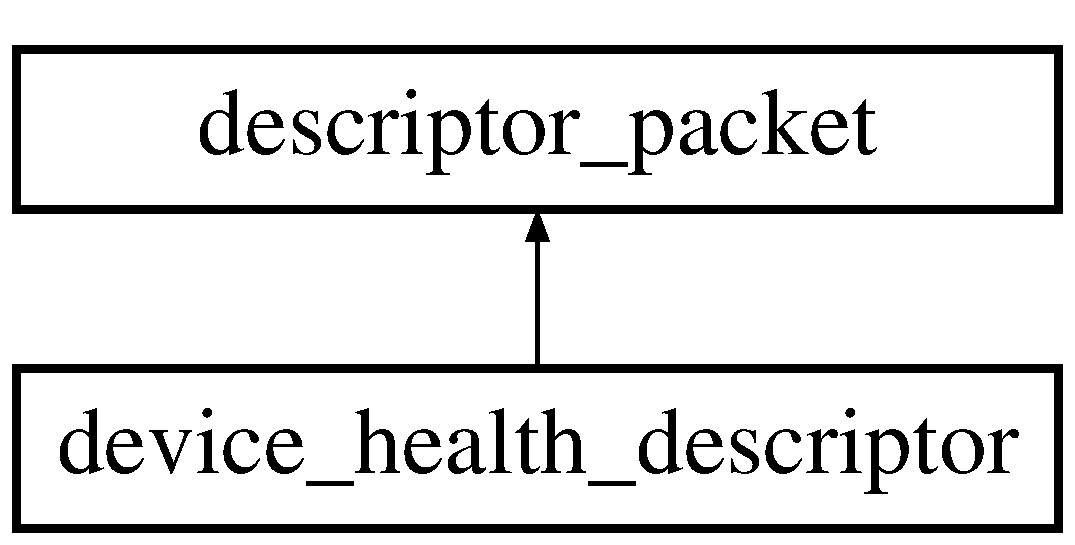
\includegraphics[height=2.000000cm]{structdevice__health__descriptor}
\end{center}
\end{figure}
\subsection*{Public Member Functions}
\begin{DoxyCompactItemize}
\item 
\hyperlink{structdevice__health__descriptor_a32127304d96ae4b44a59f6403d1f6ca0}{device\-\_\-health\-\_\-descriptor} ()
\item 
virtual std\-::string \hyperlink{structdevice__health__descriptor_a54b8725863d9ca6c640a8eb5e557109f}{type} ()
\end{DoxyCompactItemize}
\subsection*{Additional Inherited Members}


\subsection{Constructor \& Destructor Documentation}
\hypertarget{structdevice__health__descriptor_a32127304d96ae4b44a59f6403d1f6ca0}{\index{device\-\_\-health\-\_\-descriptor@{device\-\_\-health\-\_\-descriptor}!device\-\_\-health\-\_\-descriptor@{device\-\_\-health\-\_\-descriptor}}
\index{device\-\_\-health\-\_\-descriptor@{device\-\_\-health\-\_\-descriptor}!device_health_descriptor@{device\-\_\-health\-\_\-descriptor}}
\subsubsection[{device\-\_\-health\-\_\-descriptor}]{\setlength{\rightskip}{0pt plus 5cm}device\-\_\-health\-\_\-descriptor\-::device\-\_\-health\-\_\-descriptor (
\begin{DoxyParamCaption}
{}
\end{DoxyParamCaption}
)\hspace{0.3cm}{\ttfamily [inline]}}}\label{structdevice__health__descriptor_a32127304d96ae4b44a59f6403d1f6ca0}


\subsection{Member Function Documentation}
\hypertarget{structdevice__health__descriptor_a54b8725863d9ca6c640a8eb5e557109f}{\index{device\-\_\-health\-\_\-descriptor@{device\-\_\-health\-\_\-descriptor}!type@{type}}
\index{type@{type}!device_health_descriptor@{device\-\_\-health\-\_\-descriptor}}
\subsubsection[{type}]{\setlength{\rightskip}{0pt plus 5cm}virtual std\-::string device\-\_\-health\-\_\-descriptor\-::type (
\begin{DoxyParamCaption}
{}
\end{DoxyParamCaption}
)\hspace{0.3cm}{\ttfamily [inline]}, {\ttfamily [virtual]}}}\label{structdevice__health__descriptor_a54b8725863d9ca6c640a8eb5e557109f}


Implements \hyperlink{structdescriptor__packet_ad08369aae987f91544cee5e8f2267f2f}{descriptor\-\_\-packet}.



The documentation for this struct was generated from the following file\-:\begin{DoxyCompactItemize}
\item 
/home/dprandle/\-Documents/code/ctrlmod/include/\hyperlink{edrplidar__packets_8h}{edrplidar\-\_\-packets.\-h}\end{DoxyCompactItemize}

\hypertarget{structdevice__health__request}{\section{device\-\_\-health\-\_\-request Struct Reference}
\label{structdevice__health__request}\index{device\-\_\-health\-\_\-request@{device\-\_\-health\-\_\-request}}
}


{\ttfamily \#include $<$edrplidar\-\_\-packets.\-h$>$}

Inheritance diagram for device\-\_\-health\-\_\-request\-:\begin{figure}[H]
\begin{center}
\leavevmode
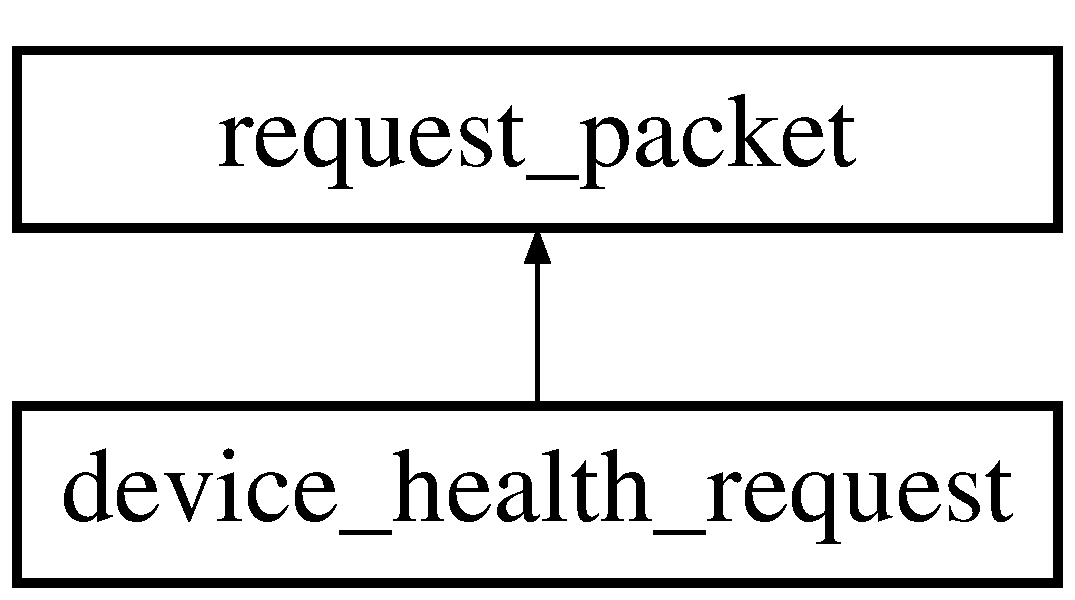
\includegraphics[height=2.000000cm]{structdevice__health__request}
\end{center}
\end{figure}
\subsection*{Public Member Functions}
\begin{DoxyCompactItemize}
\item 
\hyperlink{structdevice__health__request_a6d59496ff8a8bc154801b0f93a419088}{device\-\_\-health\-\_\-request} ()
\end{DoxyCompactItemize}
\subsection*{Additional Inherited Members}


\subsection{Constructor \& Destructor Documentation}
\hypertarget{structdevice__health__request_a6d59496ff8a8bc154801b0f93a419088}{\index{device\-\_\-health\-\_\-request@{device\-\_\-health\-\_\-request}!device\-\_\-health\-\_\-request@{device\-\_\-health\-\_\-request}}
\index{device\-\_\-health\-\_\-request@{device\-\_\-health\-\_\-request}!device_health_request@{device\-\_\-health\-\_\-request}}
\subsubsection[{device\-\_\-health\-\_\-request}]{\setlength{\rightskip}{0pt plus 5cm}device\-\_\-health\-\_\-request\-::device\-\_\-health\-\_\-request (
\begin{DoxyParamCaption}
{}
\end{DoxyParamCaption}
)\hspace{0.3cm}{\ttfamily [inline]}}}\label{structdevice__health__request_a6d59496ff8a8bc154801b0f93a419088}


The documentation for this struct was generated from the following file\-:\begin{DoxyCompactItemize}
\item 
/home/dprandle/\-Documents/code/ctrlmod/include/\hyperlink{edrplidar__packets_8h}{edrplidar\-\_\-packets.\-h}\end{DoxyCompactItemize}

\hypertarget{structdevice__info__descriptor}{\section{device\-\_\-info\-\_\-descriptor Struct Reference}
\label{structdevice__info__descriptor}\index{device\-\_\-info\-\_\-descriptor@{device\-\_\-info\-\_\-descriptor}}
}


{\ttfamily \#include $<$edrplidar\-\_\-packets.\-h$>$}

Inheritance diagram for device\-\_\-info\-\_\-descriptor\-:\begin{figure}[H]
\begin{center}
\leavevmode
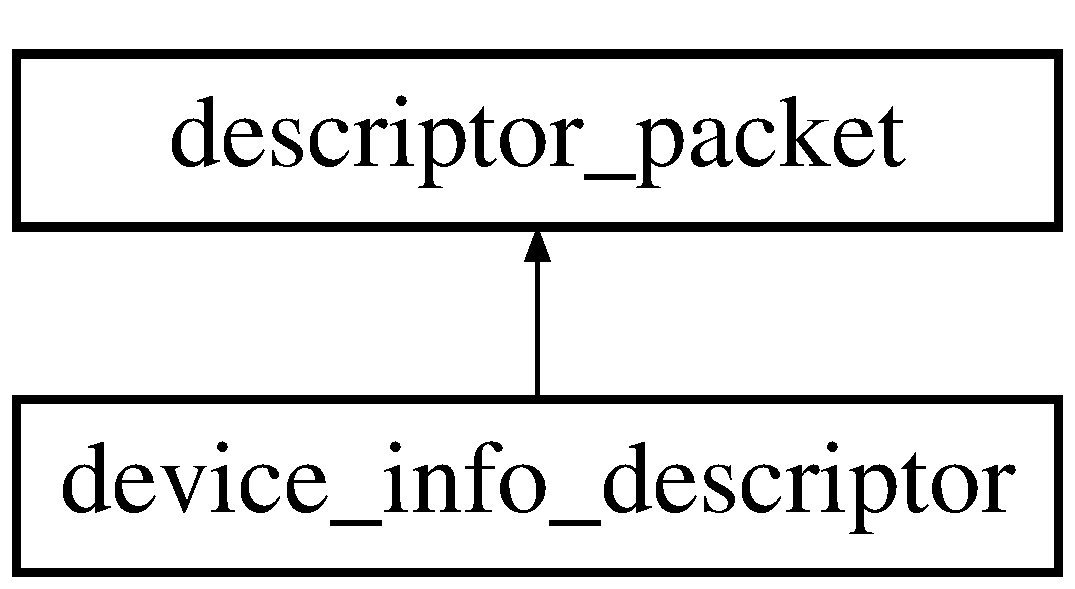
\includegraphics[height=2.000000cm]{structdevice__info__descriptor}
\end{center}
\end{figure}
\subsection*{Public Member Functions}
\begin{DoxyCompactItemize}
\item 
\hyperlink{structdevice__info__descriptor_a6475aa8a0c1ae086359990c5c128a8bd}{device\-\_\-info\-\_\-descriptor} ()
\item 
virtual std\-::string \hyperlink{structdevice__info__descriptor_a52fb00aa7ddd64fb130622f1cae6f4e2}{type} ()
\end{DoxyCompactItemize}
\subsection*{Additional Inherited Members}


\subsection{Constructor \& Destructor Documentation}
\hypertarget{structdevice__info__descriptor_a6475aa8a0c1ae086359990c5c128a8bd}{\index{device\-\_\-info\-\_\-descriptor@{device\-\_\-info\-\_\-descriptor}!device\-\_\-info\-\_\-descriptor@{device\-\_\-info\-\_\-descriptor}}
\index{device\-\_\-info\-\_\-descriptor@{device\-\_\-info\-\_\-descriptor}!device_info_descriptor@{device\-\_\-info\-\_\-descriptor}}
\subsubsection[{device\-\_\-info\-\_\-descriptor}]{\setlength{\rightskip}{0pt plus 5cm}device\-\_\-info\-\_\-descriptor\-::device\-\_\-info\-\_\-descriptor (
\begin{DoxyParamCaption}
{}
\end{DoxyParamCaption}
)\hspace{0.3cm}{\ttfamily [inline]}}}\label{structdevice__info__descriptor_a6475aa8a0c1ae086359990c5c128a8bd}


\subsection{Member Function Documentation}
\hypertarget{structdevice__info__descriptor_a52fb00aa7ddd64fb130622f1cae6f4e2}{\index{device\-\_\-info\-\_\-descriptor@{device\-\_\-info\-\_\-descriptor}!type@{type}}
\index{type@{type}!device_info_descriptor@{device\-\_\-info\-\_\-descriptor}}
\subsubsection[{type}]{\setlength{\rightskip}{0pt plus 5cm}virtual std\-::string device\-\_\-info\-\_\-descriptor\-::type (
\begin{DoxyParamCaption}
{}
\end{DoxyParamCaption}
)\hspace{0.3cm}{\ttfamily [inline]}, {\ttfamily [virtual]}}}\label{structdevice__info__descriptor_a52fb00aa7ddd64fb130622f1cae6f4e2}


Implements \hyperlink{structdescriptor__packet_ad08369aae987f91544cee5e8f2267f2f}{descriptor\-\_\-packet}.



The documentation for this struct was generated from the following file\-:\begin{DoxyCompactItemize}
\item 
/home/dprandle/\-Documents/code/ctrlmod/include/\hyperlink{edrplidar__packets_8h}{edrplidar\-\_\-packets.\-h}\end{DoxyCompactItemize}

\hypertarget{structdevice__info__request}{\section{device\-\_\-info\-\_\-request Struct Reference}
\label{structdevice__info__request}\index{device\-\_\-info\-\_\-request@{device\-\_\-info\-\_\-request}}
}


{\ttfamily \#include $<$edrplidar\-\_\-packets.\-h$>$}

Inheritance diagram for device\-\_\-info\-\_\-request\-:\begin{figure}[H]
\begin{center}
\leavevmode
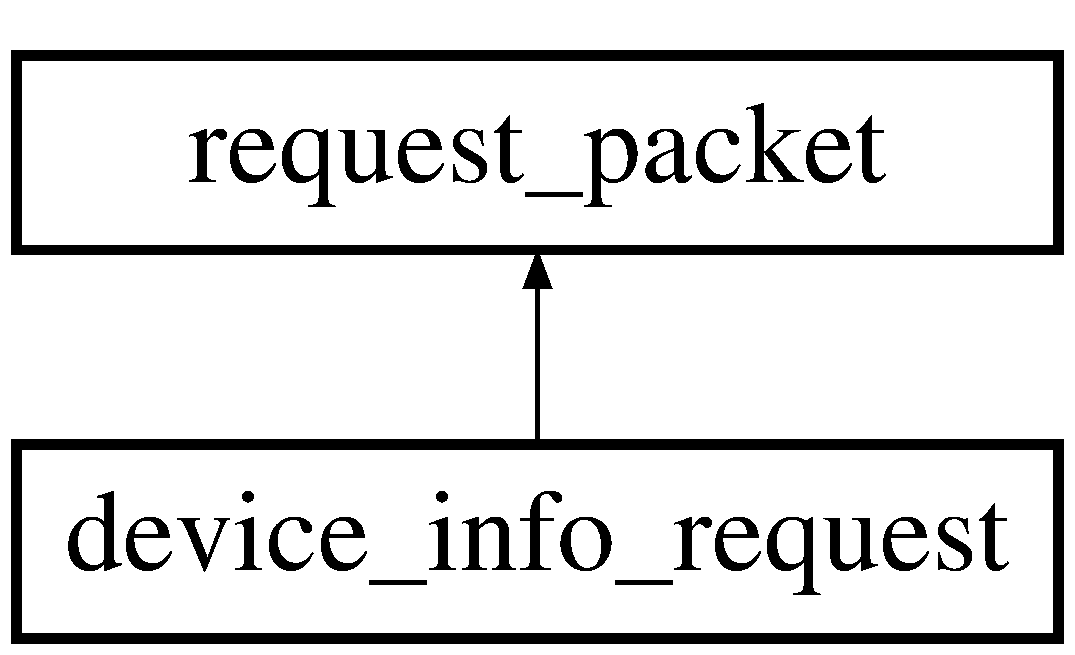
\includegraphics[height=2.000000cm]{structdevice__info__request}
\end{center}
\end{figure}
\subsection*{Public Member Functions}
\begin{DoxyCompactItemize}
\item 
\hyperlink{structdevice__info__request_aad2fe393ec65cb2822beff09ed1b8871}{device\-\_\-info\-\_\-request} ()
\end{DoxyCompactItemize}
\subsection*{Additional Inherited Members}


\subsection{Constructor \& Destructor Documentation}
\hypertarget{structdevice__info__request_aad2fe393ec65cb2822beff09ed1b8871}{\index{device\-\_\-info\-\_\-request@{device\-\_\-info\-\_\-request}!device\-\_\-info\-\_\-request@{device\-\_\-info\-\_\-request}}
\index{device\-\_\-info\-\_\-request@{device\-\_\-info\-\_\-request}!device_info_request@{device\-\_\-info\-\_\-request}}
\subsubsection[{device\-\_\-info\-\_\-request}]{\setlength{\rightskip}{0pt plus 5cm}device\-\_\-info\-\_\-request\-::device\-\_\-info\-\_\-request (
\begin{DoxyParamCaption}
{}
\end{DoxyParamCaption}
)\hspace{0.3cm}{\ttfamily [inline]}}}\label{structdevice__info__request_aad2fe393ec65cb2822beff09ed1b8871}


The documentation for this struct was generated from the following file\-:\begin{DoxyCompactItemize}
\item 
/home/dprandle/\-Documents/code/ctrlmod/include/\hyperlink{edrplidar__packets_8h}{edrplidar\-\_\-packets.\-h}\end{DoxyCompactItemize}

\hypertarget{structedcallback}{\section{edcallback Struct Reference}
\label{structedcallback}\index{edcallback@{edcallback}}
}


{\ttfamily \#include $<$edcallback.\-h$>$}

Inheritance diagram for edcallback\-:\begin{figure}[H]
\begin{center}
\leavevmode
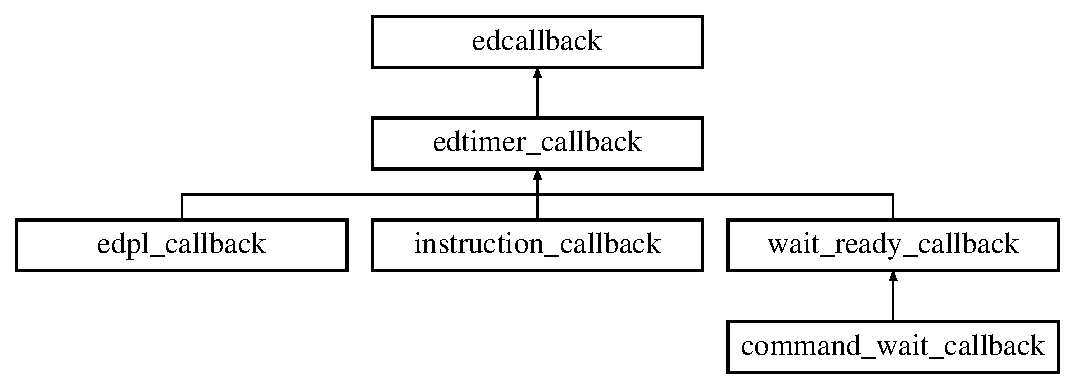
\includegraphics[height=4.000000cm]{structedcallback}
\end{center}
\end{figure}
\subsection*{Public Member Functions}
\begin{DoxyCompactItemize}
\item 
virtual \hyperlink{structedcallback_a42cabca3099d69b2960d70bdf14c013c}{$\sim$edcallback} ()
\item 
virtual void \hyperlink{structedcallback_ab8003af2178e58a94f53370b1f48a313}{exec} ()=0
\end{DoxyCompactItemize}


\subsection{Constructor \& Destructor Documentation}
\hypertarget{structedcallback_a42cabca3099d69b2960d70bdf14c013c}{\index{edcallback@{edcallback}!$\sim$edcallback@{$\sim$edcallback}}
\index{$\sim$edcallback@{$\sim$edcallback}!edcallback@{edcallback}}
\subsubsection[{$\sim$edcallback}]{\setlength{\rightskip}{0pt plus 5cm}virtual edcallback\-::$\sim$edcallback (
\begin{DoxyParamCaption}
{}
\end{DoxyParamCaption}
)\hspace{0.3cm}{\ttfamily [inline]}, {\ttfamily [virtual]}}}\label{structedcallback_a42cabca3099d69b2960d70bdf14c013c}


\subsection{Member Function Documentation}
\hypertarget{structedcallback_ab8003af2178e58a94f53370b1f48a313}{\index{edcallback@{edcallback}!exec@{exec}}
\index{exec@{exec}!edcallback@{edcallback}}
\subsubsection[{exec}]{\setlength{\rightskip}{0pt plus 5cm}virtual void edcallback\-::exec (
\begin{DoxyParamCaption}
{}
\end{DoxyParamCaption}
)\hspace{0.3cm}{\ttfamily [pure virtual]}}}\label{structedcallback_ab8003af2178e58a94f53370b1f48a313}


Implemented in \hyperlink{structcommand__wait__callback_ae5ab034230cd73f6203cee386ba1993c}{command\-\_\-wait\-\_\-callback}, \hyperlink{structinstruction__callback_a74abfad8ac25461bb99e11fba10516c2}{instruction\-\_\-callback}, \hyperlink{structedpl__callback_a23c8aacf97d5a080af1f7d84439122c8}{edpl\-\_\-callback}, and \hyperlink{structwait__ready__callback_a305d57ffdd8bc5d3682dfa4a83431708}{wait\-\_\-ready\-\_\-callback}.



The documentation for this struct was generated from the following file\-:\begin{DoxyCompactItemize}
\item 
/home/dprandle/\-Documents/code/ctrlmod/include/\hyperlink{edcallback_8h}{edcallback.\-h}\end{DoxyCompactItemize}

\hypertarget{classedcomm__system}{\section{edcomm\-\_\-system Class Reference}
\label{classedcomm__system}\index{edcomm\-\_\-system@{edcomm\-\_\-system}}
}


{\ttfamily \#include $<$edcomm\-\_\-system.\-h$>$}

Inheritance diagram for edcomm\-\_\-system\-:\begin{figure}[H]
\begin{center}
\leavevmode
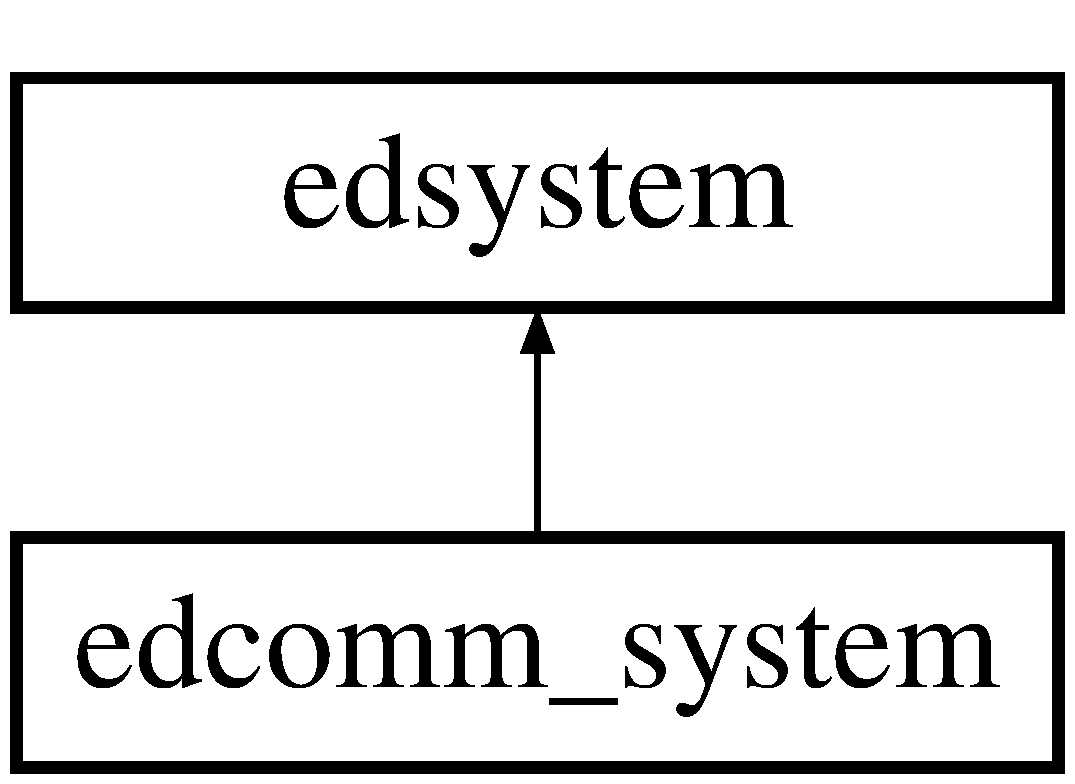
\includegraphics[height=2.000000cm]{classedcomm__system}
\end{center}
\end{figure}
\subsection*{Public Member Functions}
\begin{DoxyCompactItemize}
\item 
\hyperlink{classedcomm__system_af0ff75511346286c460c8032f55b07ae}{edcomm\-\_\-system} ()
\item 
virtual \hyperlink{classedcomm__system_a15e21d845f4491cd2f8d82fb0924b580}{$\sim$edcomm\-\_\-system} ()
\item 
virtual void \hyperlink{classedcomm__system_a07f81f18aeca00b88928a8aec7b3129e}{init} ()
\item 
virtual void \hyperlink{classedcomm__system_ad9bdfd2845a3156f5d010e99f8fbed07}{release} ()
\item 
virtual bool \hyperlink{classedcomm__system_ad3b79f16dd77b5ae458cc360550e99cd}{process} (\hyperlink{structedmessage}{edmessage} $\ast$msg)
\item 
uint16\-\_\-t \hyperlink{classedcomm__system_ac7f39247c0f1ae2023adf9562dbc7c81}{port} ()
\item 
void \hyperlink{classedcomm__system_a36087648658a44860a8905d4b979c8fe}{set\-\_\-port} (uint16\-\_\-t port\-\_\-)
\item 
virtual void \hyperlink{classedcomm__system_adc9ffc8199070ad0d836a447005a4e1e}{update} ()
\item 
uint32\-\_\-t \hyperlink{classedcomm__system_ae9196f8b00b7e5d5a26075c4311b058c}{recv\-From\-Clients} (uint8\-\_\-t $\ast$data, uint32\-\_\-t max\-\_\-size)
\item 
void \hyperlink{classedcomm__system_a91aa83b31bc197b2f0ec1c5600f4ec9f}{send\-To\-Clients} (uint8\-\_\-t $\ast$data, uint32\-\_\-t size)
\item 
virtual std\-::string \hyperlink{classedcomm__system_a61e1243fba536c8263ba93367cd5a2a7}{typestr} ()
\end{DoxyCompactItemize}
\subsection*{Static Public Member Functions}
\begin{DoxyCompactItemize}
\item 
static std\-::string \hyperlink{classedcomm__system_a0e58236d155e30df3cc55de56023cdd5}{Type\-String} ()
\end{DoxyCompactItemize}


\subsection{Constructor \& Destructor Documentation}
\hypertarget{classedcomm__system_af0ff75511346286c460c8032f55b07ae}{\index{edcomm\-\_\-system@{edcomm\-\_\-system}!edcomm\-\_\-system@{edcomm\-\_\-system}}
\index{edcomm\-\_\-system@{edcomm\-\_\-system}!edcomm_system@{edcomm\-\_\-system}}
\subsubsection[{edcomm\-\_\-system}]{\setlength{\rightskip}{0pt plus 5cm}edcomm\-\_\-system\-::edcomm\-\_\-system (
\begin{DoxyParamCaption}
{}
\end{DoxyParamCaption}
)}}\label{classedcomm__system_af0ff75511346286c460c8032f55b07ae}
\hypertarget{classedcomm__system_a15e21d845f4491cd2f8d82fb0924b580}{\index{edcomm\-\_\-system@{edcomm\-\_\-system}!$\sim$edcomm\-\_\-system@{$\sim$edcomm\-\_\-system}}
\index{$\sim$edcomm\-\_\-system@{$\sim$edcomm\-\_\-system}!edcomm_system@{edcomm\-\_\-system}}
\subsubsection[{$\sim$edcomm\-\_\-system}]{\setlength{\rightskip}{0pt plus 5cm}edcomm\-\_\-system\-::$\sim$edcomm\-\_\-system (
\begin{DoxyParamCaption}
{}
\end{DoxyParamCaption}
)\hspace{0.3cm}{\ttfamily [virtual]}}}\label{classedcomm__system_a15e21d845f4491cd2f8d82fb0924b580}


\subsection{Member Function Documentation}
\hypertarget{classedcomm__system_a07f81f18aeca00b88928a8aec7b3129e}{\index{edcomm\-\_\-system@{edcomm\-\_\-system}!init@{init}}
\index{init@{init}!edcomm_system@{edcomm\-\_\-system}}
\subsubsection[{init}]{\setlength{\rightskip}{0pt plus 5cm}void edcomm\-\_\-system\-::init (
\begin{DoxyParamCaption}
{}
\end{DoxyParamCaption}
)\hspace{0.3cm}{\ttfamily [virtual]}}}\label{classedcomm__system_a07f81f18aeca00b88928a8aec7b3129e}


Implements \hyperlink{classedsystem_a4c70e3568064941607fb220aea826a56}{edsystem}.

\hypertarget{classedcomm__system_ac7f39247c0f1ae2023adf9562dbc7c81}{\index{edcomm\-\_\-system@{edcomm\-\_\-system}!port@{port}}
\index{port@{port}!edcomm_system@{edcomm\-\_\-system}}
\subsubsection[{port}]{\setlength{\rightskip}{0pt plus 5cm}uint16\-\_\-t edcomm\-\_\-system\-::port (
\begin{DoxyParamCaption}
{}
\end{DoxyParamCaption}
)}}\label{classedcomm__system_ac7f39247c0f1ae2023adf9562dbc7c81}
\hypertarget{classedcomm__system_ad3b79f16dd77b5ae458cc360550e99cd}{\index{edcomm\-\_\-system@{edcomm\-\_\-system}!process@{process}}
\index{process@{process}!edcomm_system@{edcomm\-\_\-system}}
\subsubsection[{process}]{\setlength{\rightskip}{0pt plus 5cm}bool edcomm\-\_\-system\-::process (
\begin{DoxyParamCaption}
\item[{{\bf edmessage} $\ast$}]{msg}
\end{DoxyParamCaption}
)\hspace{0.3cm}{\ttfamily [virtual]}}}\label{classedcomm__system_ad3b79f16dd77b5ae458cc360550e99cd}


Implements \hyperlink{classedsystem_a9d7a0547c702af1572ed8a1f5434fa0a}{edsystem}.

\hypertarget{classedcomm__system_ae9196f8b00b7e5d5a26075c4311b058c}{\index{edcomm\-\_\-system@{edcomm\-\_\-system}!recv\-From\-Clients@{recv\-From\-Clients}}
\index{recv\-From\-Clients@{recv\-From\-Clients}!edcomm_system@{edcomm\-\_\-system}}
\subsubsection[{recv\-From\-Clients}]{\setlength{\rightskip}{0pt plus 5cm}uint32\-\_\-t edcomm\-\_\-system\-::recv\-From\-Clients (
\begin{DoxyParamCaption}
\item[{uint8\-\_\-t $\ast$}]{data, }
\item[{uint32\-\_\-t}]{max\-\_\-size}
\end{DoxyParamCaption}
)}}\label{classedcomm__system_ae9196f8b00b7e5d5a26075c4311b058c}
\hypertarget{classedcomm__system_ad9bdfd2845a3156f5d010e99f8fbed07}{\index{edcomm\-\_\-system@{edcomm\-\_\-system}!release@{release}}
\index{release@{release}!edcomm_system@{edcomm\-\_\-system}}
\subsubsection[{release}]{\setlength{\rightskip}{0pt plus 5cm}void edcomm\-\_\-system\-::release (
\begin{DoxyParamCaption}
{}
\end{DoxyParamCaption}
)\hspace{0.3cm}{\ttfamily [virtual]}}}\label{classedcomm__system_ad9bdfd2845a3156f5d010e99f8fbed07}


Implements \hyperlink{classedsystem_af40ac185ca4a8efd6777fdb4c65880ea}{edsystem}.

\hypertarget{classedcomm__system_a91aa83b31bc197b2f0ec1c5600f4ec9f}{\index{edcomm\-\_\-system@{edcomm\-\_\-system}!send\-To\-Clients@{send\-To\-Clients}}
\index{send\-To\-Clients@{send\-To\-Clients}!edcomm_system@{edcomm\-\_\-system}}
\subsubsection[{send\-To\-Clients}]{\setlength{\rightskip}{0pt plus 5cm}void edcomm\-\_\-system\-::send\-To\-Clients (
\begin{DoxyParamCaption}
\item[{uint8\-\_\-t $\ast$}]{data, }
\item[{uint32\-\_\-t}]{size}
\end{DoxyParamCaption}
)}}\label{classedcomm__system_a91aa83b31bc197b2f0ec1c5600f4ec9f}
\hypertarget{classedcomm__system_a36087648658a44860a8905d4b979c8fe}{\index{edcomm\-\_\-system@{edcomm\-\_\-system}!set\-\_\-port@{set\-\_\-port}}
\index{set\-\_\-port@{set\-\_\-port}!edcomm_system@{edcomm\-\_\-system}}
\subsubsection[{set\-\_\-port}]{\setlength{\rightskip}{0pt plus 5cm}void edcomm\-\_\-system\-::set\-\_\-port (
\begin{DoxyParamCaption}
\item[{uint16\-\_\-t}]{port\-\_\-}
\end{DoxyParamCaption}
)}}\label{classedcomm__system_a36087648658a44860a8905d4b979c8fe}
\hypertarget{classedcomm__system_a61e1243fba536c8263ba93367cd5a2a7}{\index{edcomm\-\_\-system@{edcomm\-\_\-system}!typestr@{typestr}}
\index{typestr@{typestr}!edcomm_system@{edcomm\-\_\-system}}
\subsubsection[{typestr}]{\setlength{\rightskip}{0pt plus 5cm}virtual std\-::string edcomm\-\_\-system\-::typestr (
\begin{DoxyParamCaption}
{}
\end{DoxyParamCaption}
)\hspace{0.3cm}{\ttfamily [inline]}, {\ttfamily [virtual]}}}\label{classedcomm__system_a61e1243fba536c8263ba93367cd5a2a7}


Implements \hyperlink{classedsystem_a19dc65111f9a38259fcafba3a32a646d}{edsystem}.

\hypertarget{classedcomm__system_a0e58236d155e30df3cc55de56023cdd5}{\index{edcomm\-\_\-system@{edcomm\-\_\-system}!Type\-String@{Type\-String}}
\index{Type\-String@{Type\-String}!edcomm_system@{edcomm\-\_\-system}}
\subsubsection[{Type\-String}]{\setlength{\rightskip}{0pt plus 5cm}static std\-::string edcomm\-\_\-system\-::\-Type\-String (
\begin{DoxyParamCaption}
{}
\end{DoxyParamCaption}
)\hspace{0.3cm}{\ttfamily [inline]}, {\ttfamily [static]}}}\label{classedcomm__system_a0e58236d155e30df3cc55de56023cdd5}
\hypertarget{classedcomm__system_adc9ffc8199070ad0d836a447005a4e1e}{\index{edcomm\-\_\-system@{edcomm\-\_\-system}!update@{update}}
\index{update@{update}!edcomm_system@{edcomm\-\_\-system}}
\subsubsection[{update}]{\setlength{\rightskip}{0pt plus 5cm}void edcomm\-\_\-system\-::update (
\begin{DoxyParamCaption}
{}
\end{DoxyParamCaption}
)\hspace{0.3cm}{\ttfamily [virtual]}}}\label{classedcomm__system_adc9ffc8199070ad0d836a447005a4e1e}


Implements \hyperlink{classedsystem_afd5308dc71350fe4e239cac5fb1bdbe9}{edsystem}.



The documentation for this class was generated from the following files\-:\begin{DoxyCompactItemize}
\item 
/home/dprandle/\-Documents/code/ctrlmod/include/\hyperlink{edcomm__system_8h}{edcomm\-\_\-system.\-h}\item 
/home/dprandle/\-Documents/code/ctrlmod/src/\hyperlink{edcomm__system_8cpp}{edcomm\-\_\-system.\-cpp}\end{DoxyCompactItemize}

\hypertarget{classedi2c}{\section{edi2c Class Reference}
\label{classedi2c}\index{edi2c@{edi2c}}
}


\hyperlink{classedi2c}{edi2c}  




{\ttfamily \#include $<$edi2c.\-h$>$}

Inheritance diagram for edi2c\-:\begin{figure}[H]
\begin{center}
\leavevmode
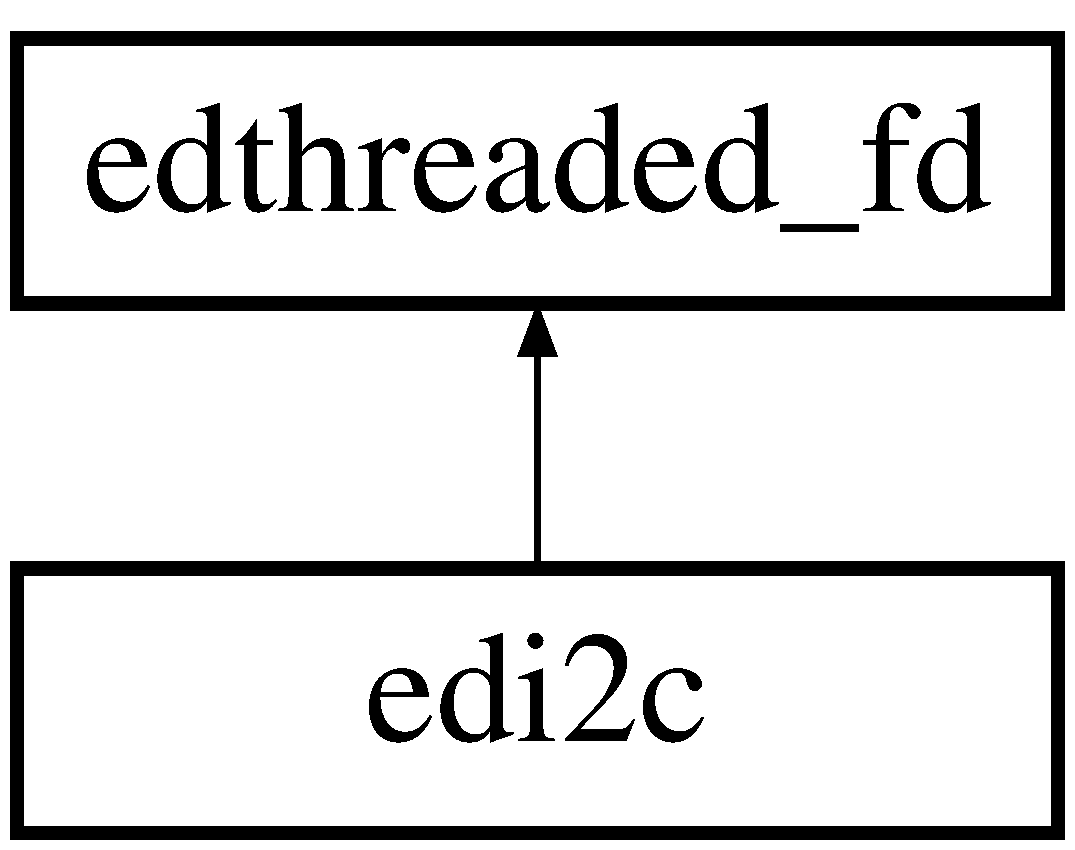
\includegraphics[height=2.000000cm]{classedi2c}
\end{center}
\end{figure}
\subsection*{Public Member Functions}
\begin{DoxyCompactItemize}
\item 
\hyperlink{classedi2c_a1af1282b3a5c22f8690a2758bf3720bb}{edi2c} (uint32\-\_\-t adapter\-Num=1)
\item 
\hyperlink{classedi2c_a35e32414433c5b66109ade0da6f98079}{$\sim$edi2c} ()
\item 
bool \hyperlink{classedi2c_a24e263124eb80f5c841f8b804b69e943}{command\-\_\-read} (uint8\-\_\-t reg, uint32\-\_\-t bytes\-\_\-to\-\_\-read)
\begin{DoxyCompactList}\small\item\em command\-\_\-read \end{DoxyCompactList}\item 
void \hyperlink{classedi2c_a9c9e5492ab0aa7361e3871616dc1ee5e}{enable\-\_\-smbus} (bool enable)
\begin{DoxyCompactList}\small\item\em enaable\-\_\-smbus \end{DoxyCompactList}\item 
uint8\-\_\-t \hyperlink{classedi2c_a53cd636c8a9fd4ca54e5b0473cc8cb84}{read\-\_\-byte} ()
\begin{DoxyCompactList}\small\item\em read\-\_\-byte \end{DoxyCompactList}\item 
uint16\-\_\-t \hyperlink{classedi2c_a2b727b09d18b70cfd0466ce4d85a858b}{read\-\_\-word} ()
\begin{DoxyCompactList}\small\item\em read\-\_\-word \end{DoxyCompactList}\item 
uint8\-\_\-t \hyperlink{classedi2c_af72f531db5a7112e6da2d9e626932519}{read\-\_\-reg\-\_\-byte} (uint8\-\_\-t reg)
\begin{DoxyCompactList}\small\item\em read\-\_\-reg\-\_\-byte \end{DoxyCompactList}\item 
int16\-\_\-t \hyperlink{classedi2c_a0f5ed693ef1a4ecf95552d5fa459d839}{read\-\_\-reg\-\_\-word} (uint8\-\_\-t reg)
\begin{DoxyCompactList}\small\item\em read\-\_\-reg\-\_\-word \end{DoxyCompactList}\item 
void \hyperlink{classedi2c_acd7b0631883fca709e2d65d184c29826}{read\-\_\-reg\-\_\-bytes} (uint8\-\_\-t reg, uint8\-\_\-t $\ast$buffer, uint32\-\_\-t size)
\begin{DoxyCompactList}\small\item\em read\-\_\-reg\-\_\-bytes \end{DoxyCompactList}\item 
uint16\-\_\-t \hyperlink{classedi2c_a6e9e5641194e8cd076e6cedfc6673ed3}{read\-\_\-delay} ()
\begin{DoxyCompactList}\small\item\em read\-\_\-delay \end{DoxyCompactList}\item 
uint16\-\_\-t \hyperlink{classedi2c_ac72e569257fb740b0431d8ce5fa5a3d5}{write\-\_\-delay} ()
\begin{DoxyCompactList}\small\item\em write\-\_\-delay \end{DoxyCompactList}\item 
void \hyperlink{classedi2c_af56980b466616331c3a953f6b5c034ed}{set\-\_\-read\-\_\-delay} (uint16\-\_\-t ms)
\begin{DoxyCompactList}\small\item\em set\-\_\-read\-\_\-delay \end{DoxyCompactList}\item 
void \hyperlink{classedi2c_a2e9079f183b0f087b55398c55b38b97f}{set\-\_\-write\-\_\-delay} (uint16\-\_\-t ms)
\item 
void \hyperlink{classedi2c_a938ee09d908469548b31f6561d906528}{set\-\_\-target\-\_\-address} (int32\-\_\-t addr)
\begin{DoxyCompactList}\small\item\em set\-\_\-target\-\_\-address \end{DoxyCompactList}\item 
bool \hyperlink{classedi2c_a6888361fe70d4c9110113e4a45912f7c}{smbus\-\_\-enabled} ()
\begin{DoxyCompactList}\small\item\em smbus\-\_\-enables \end{DoxyCompactList}\item 
bool \hyperlink{classedi2c_ad0e06417e0b488df02b1864d316d72c1}{start} ()
\begin{DoxyCompactList}\small\item\em start \end{DoxyCompactList}\item 
int32\-\_\-t \hyperlink{classedi2c_aba709407bd42c5dcee257726dff12526}{target\-\_\-address} ()
\item 
bool \hyperlink{classedi2c_a245ebdd9ac48c5671de79bebccf29e97}{write\-\_\-byte} (uint8\-\_\-t byte)
\item 
bool \hyperlink{classedi2c_a31d8723f4c2678c2709fdff8e0b36f67}{write\-\_\-word} (uint16\-\_\-t word)
\item 
bool \hyperlink{classedi2c_ad54e95daa301895c7be525768ce0512a}{write\-\_\-reg\-\_\-byte} (uint8\-\_\-t reg, uint8\-\_\-t byte)
\item 
bool \hyperlink{classedi2c_a220239a9eb19a4e0cb760e81259a25a4}{write\-\_\-reg\-\_\-word} (uint8\-\_\-t reg, int16\-\_\-t word)
\item 
bool \hyperlink{classedi2c_a19785c35d613e72285234d194a294a09}{write\-\_\-reg\-\_\-bytes} (uint8\-\_\-t reg, uint8\-\_\-t $\ast$bytes, uint32\-\_\-t size)
\end{DoxyCompactItemize}
\subsection*{Additional Inherited Members}


\subsection{Detailed Description}
\hyperlink{classedi2c}{edi2c} 

Creates a new thread to run all communication transactions using i2c protocol. The way to use this class is just like any other \char`\"{}edthreaded\-\_\-fd\char`\"{} subclass -\/ with a main exception\-: The read\-\_\-$\ast$ functions are all blocking. The read function itself is not blocking. If you want to read a value from a register in a non blocking fashion then you must use command\-\_\-read instead of read\-\_\-$\ast$ functions. The command\-\_\-read function takes how many bytes to read as a parameter -\/ and you can access theses bytes with \char`\"{}read\char`\"{}. 

\subsection{Constructor \& Destructor Documentation}
\hypertarget{classedi2c_a1af1282b3a5c22f8690a2758bf3720bb}{\index{edi2c@{edi2c}!edi2c@{edi2c}}
\index{edi2c@{edi2c}!edi2c@{edi2c}}
\subsubsection[{edi2c}]{\setlength{\rightskip}{0pt plus 5cm}edi2c\-::edi2c (
\begin{DoxyParamCaption}
\item[{uint32\-\_\-t}]{adapter\-Num = {\ttfamily 1}}
\end{DoxyParamCaption}
)}}\label{classedi2c_a1af1282b3a5c22f8690a2758bf3720bb}
\hypertarget{classedi2c_a35e32414433c5b66109ade0da6f98079}{\index{edi2c@{edi2c}!$\sim$edi2c@{$\sim$edi2c}}
\index{$\sim$edi2c@{$\sim$edi2c}!edi2c@{edi2c}}
\subsubsection[{$\sim$edi2c}]{\setlength{\rightskip}{0pt plus 5cm}edi2c\-::$\sim$edi2c (
\begin{DoxyParamCaption}
{}
\end{DoxyParamCaption}
)}}\label{classedi2c_a35e32414433c5b66109ade0da6f98079}


\subsection{Member Function Documentation}
\hypertarget{classedi2c_a24e263124eb80f5c841f8b804b69e943}{\index{edi2c@{edi2c}!command\-\_\-read@{command\-\_\-read}}
\index{command\-\_\-read@{command\-\_\-read}!edi2c@{edi2c}}
\subsubsection[{command\-\_\-read}]{\setlength{\rightskip}{0pt plus 5cm}bool edi2c\-::command\-\_\-read (
\begin{DoxyParamCaption}
\item[{uint8\-\_\-t}]{reg, }
\item[{uint32\-\_\-t}]{bytes\-\_\-to\-\_\-read}
\end{DoxyParamCaption}
)}}\label{classedi2c_a24e263124eb80f5c841f8b804b69e943}


command\-\_\-read 

Read from a register in a non-\/blocking fashion -\/ once the bytes have been read they will be available through read function. Nothing more will be written to the i2c device until bytes\-\_\-to\-\_\-read bytes have been read or the timeout period of time has been reached.


\begin{DoxyParams}{Parameters}
{\em reg} & register to read bytes from \\
\hline
{\em bytes\-\_\-to\-\_\-read} & amount of bytes to read\\
\hline
\end{DoxyParams}
\begin{DoxyReturn}{Returns}
Whether the command was successful or not. Will not be, for example, if no device is connected. 
\end{DoxyReturn}
\hypertarget{classedi2c_a9c9e5492ab0aa7361e3871616dc1ee5e}{\index{edi2c@{edi2c}!enable\-\_\-smbus@{enable\-\_\-smbus}}
\index{enable\-\_\-smbus@{enable\-\_\-smbus}!edi2c@{edi2c}}
\subsubsection[{enable\-\_\-smbus}]{\setlength{\rightskip}{0pt plus 5cm}void edi2c\-::enable\-\_\-smbus (
\begin{DoxyParamCaption}
\item[{bool}]{enable}
\end{DoxyParamCaption}
)}}\label{classedi2c_a9c9e5492ab0aa7361e3871616dc1ee5e}


enaable\-\_\-smbus 

Disabled by default, this will enable the smbus functions. Smbus supports more advanced styles of messaging between devices but not all devices support the smbus protocol.


\begin{DoxyParams}{Parameters}
{\em enable} & Enable (true) or disable (false) \\
\hline
\end{DoxyParams}
\hypertarget{classedi2c_a53cd636c8a9fd4ca54e5b0473cc8cb84}{\index{edi2c@{edi2c}!read\-\_\-byte@{read\-\_\-byte}}
\index{read\-\_\-byte@{read\-\_\-byte}!edi2c@{edi2c}}
\subsubsection[{read\-\_\-byte}]{\setlength{\rightskip}{0pt plus 5cm}uint8\-\_\-t edi2c\-::read\-\_\-byte (
\begin{DoxyParamCaption}
{}
\end{DoxyParamCaption}
)}}\label{classedi2c_a53cd636c8a9fd4ca54e5b0473cc8cb84}


read\-\_\-byte 

Blocks until one byte has been read or the maximum wait timeout has been reached.

\begin{DoxyReturn}{Returns}
byte that has been read 
\end{DoxyReturn}
\hypertarget{classedi2c_a6e9e5641194e8cd076e6cedfc6673ed3}{\index{edi2c@{edi2c}!read\-\_\-delay@{read\-\_\-delay}}
\index{read\-\_\-delay@{read\-\_\-delay}!edi2c@{edi2c}}
\subsubsection[{read\-\_\-delay}]{\setlength{\rightskip}{0pt plus 5cm}uint16\-\_\-t edi2c\-::read\-\_\-delay (
\begin{DoxyParamCaption}
{}
\end{DoxyParamCaption}
)}}\label{classedi2c_a6e9e5641194e8cd076e6cedfc6673ed3}


read\-\_\-delay 

\begin{DoxyReturn}{Returns}
number of milliseconds to delay the thread after each read command. 
\end{DoxyReturn}
\hypertarget{classedi2c_af72f531db5a7112e6da2d9e626932519}{\index{edi2c@{edi2c}!read\-\_\-reg\-\_\-byte@{read\-\_\-reg\-\_\-byte}}
\index{read\-\_\-reg\-\_\-byte@{read\-\_\-reg\-\_\-byte}!edi2c@{edi2c}}
\subsubsection[{read\-\_\-reg\-\_\-byte}]{\setlength{\rightskip}{0pt plus 5cm}uint8\-\_\-t edi2c\-::read\-\_\-reg\-\_\-byte (
\begin{DoxyParamCaption}
\item[{uint8\-\_\-t}]{reg}
\end{DoxyParamCaption}
)}}\label{classedi2c_af72f531db5a7112e6da2d9e626932519}


read\-\_\-reg\-\_\-byte 

Blocking read until 1 byte is read from a register.


\begin{DoxyParams}{Parameters}
{\em reg} & Register to read from\\
\hline
\end{DoxyParams}
\begin{DoxyReturn}{Returns}
Byte value read from register 
\end{DoxyReturn}
\hypertarget{classedi2c_acd7b0631883fca709e2d65d184c29826}{\index{edi2c@{edi2c}!read\-\_\-reg\-\_\-bytes@{read\-\_\-reg\-\_\-bytes}}
\index{read\-\_\-reg\-\_\-bytes@{read\-\_\-reg\-\_\-bytes}!edi2c@{edi2c}}
\subsubsection[{read\-\_\-reg\-\_\-bytes}]{\setlength{\rightskip}{0pt plus 5cm}void edi2c\-::read\-\_\-reg\-\_\-bytes (
\begin{DoxyParamCaption}
\item[{uint8\-\_\-t}]{reg, }
\item[{uint8\-\_\-t $\ast$}]{buffer, }
\item[{uint32\-\_\-t}]{size}
\end{DoxyParamCaption}
)}}\label{classedi2c_acd7b0631883fca709e2d65d184c29826}


read\-\_\-reg\-\_\-bytes 

Blocking read until size bytes has been read. This is a convenience function which is the same as calling command\-\_\-read(reg, size); int cnt = 0; while (cnt != size) cnt += read(buffer+cnt, size-\/cnt);


\begin{DoxyParams}{Parameters}
{\em reg} & Register to read bytes from \\
\hline
{\em buffer} & Buffer to store read in bytes -\/ bounds are not checked so make sure it is big enough \\
\hline
{\em size} & Number of bytes to read \\
\hline
\end{DoxyParams}
\hypertarget{classedi2c_a0f5ed693ef1a4ecf95552d5fa459d839}{\index{edi2c@{edi2c}!read\-\_\-reg\-\_\-word@{read\-\_\-reg\-\_\-word}}
\index{read\-\_\-reg\-\_\-word@{read\-\_\-reg\-\_\-word}!edi2c@{edi2c}}
\subsubsection[{read\-\_\-reg\-\_\-word}]{\setlength{\rightskip}{0pt plus 5cm}int16\-\_\-t edi2c\-::read\-\_\-reg\-\_\-word (
\begin{DoxyParamCaption}
\item[{uint8\-\_\-t}]{reg}
\end{DoxyParamCaption}
)}}\label{classedi2c_a0f5ed693ef1a4ecf95552d5fa459d839}


read\-\_\-reg\-\_\-word 

Blocking read until 1 word is read from a register


\begin{DoxyParams}{Parameters}
{\em reg} & Register to read from\\
\hline
\end{DoxyParams}
\begin{DoxyReturn}{Returns}
2 byte value read from register 
\end{DoxyReturn}
\hypertarget{classedi2c_a2b727b09d18b70cfd0466ce4d85a858b}{\index{edi2c@{edi2c}!read\-\_\-word@{read\-\_\-word}}
\index{read\-\_\-word@{read\-\_\-word}!edi2c@{edi2c}}
\subsubsection[{read\-\_\-word}]{\setlength{\rightskip}{0pt plus 5cm}uint16\-\_\-t edi2c\-::read\-\_\-word (
\begin{DoxyParamCaption}
{}
\end{DoxyParamCaption}
)}}\label{classedi2c_a2b727b09d18b70cfd0466ce4d85a858b}


read\-\_\-word 

Blocks until one word has been read or the maximum wait timeout has been reached.

\begin{DoxyReturn}{Returns}
16 bit word 
\end{DoxyReturn}
\hypertarget{classedi2c_af56980b466616331c3a953f6b5c034ed}{\index{edi2c@{edi2c}!set\-\_\-read\-\_\-delay@{set\-\_\-read\-\_\-delay}}
\index{set\-\_\-read\-\_\-delay@{set\-\_\-read\-\_\-delay}!edi2c@{edi2c}}
\subsubsection[{set\-\_\-read\-\_\-delay}]{\setlength{\rightskip}{0pt plus 5cm}void edi2c\-::set\-\_\-read\-\_\-delay (
\begin{DoxyParamCaption}
\item[{uint16\-\_\-t}]{ms}
\end{DoxyParamCaption}
)}}\label{classedi2c_af56980b466616331c3a953f6b5c034ed}


set\-\_\-read\-\_\-delay 

Set the thread read delay -\/ how many milliseconds to delay the thread after each read 
\begin{DoxyParams}{Parameters}
{\em ms} & Number of milliseconds \\
\hline
\end{DoxyParams}
\hypertarget{classedi2c_a938ee09d908469548b31f6561d906528}{\index{edi2c@{edi2c}!set\-\_\-target\-\_\-address@{set\-\_\-target\-\_\-address}}
\index{set\-\_\-target\-\_\-address@{set\-\_\-target\-\_\-address}!edi2c@{edi2c}}
\subsubsection[{set\-\_\-target\-\_\-address}]{\setlength{\rightskip}{0pt plus 5cm}void edi2c\-::set\-\_\-target\-\_\-address (
\begin{DoxyParamCaption}
\item[{int32\-\_\-t}]{addr}
\end{DoxyParamCaption}
)}}\label{classedi2c_a938ee09d908469548b31f6561d906528}


set\-\_\-target\-\_\-address 

Set the target device address -\/ all reads and writes will be done using this address 
\begin{DoxyParams}{Parameters}
{\em addr} & usually 7 bit device address for the slave (can be 10 bit) \\
\hline
\end{DoxyParams}
\hypertarget{classedi2c_a2e9079f183b0f087b55398c55b38b97f}{\index{edi2c@{edi2c}!set\-\_\-write\-\_\-delay@{set\-\_\-write\-\_\-delay}}
\index{set\-\_\-write\-\_\-delay@{set\-\_\-write\-\_\-delay}!edi2c@{edi2c}}
\subsubsection[{set\-\_\-write\-\_\-delay}]{\setlength{\rightskip}{0pt plus 5cm}void edi2c\-::set\-\_\-write\-\_\-delay (
\begin{DoxyParamCaption}
\item[{uint16\-\_\-t}]{ms}
\end{DoxyParamCaption}
)}}\label{classedi2c_a2e9079f183b0f087b55398c55b38b97f}
Set the thread write delay -\/ how many milliseconds to delay the thread after each write 
\begin{DoxyParams}{Parameters}
{\em ms} & Number of milliseconds \\
\hline
\end{DoxyParams}
\hypertarget{classedi2c_a6888361fe70d4c9110113e4a45912f7c}{\index{edi2c@{edi2c}!smbus\-\_\-enabled@{smbus\-\_\-enabled}}
\index{smbus\-\_\-enabled@{smbus\-\_\-enabled}!edi2c@{edi2c}}
\subsubsection[{smbus\-\_\-enabled}]{\setlength{\rightskip}{0pt plus 5cm}bool edi2c\-::smbus\-\_\-enabled (
\begin{DoxyParamCaption}
{}
\end{DoxyParamCaption}
)}}\label{classedi2c_a6888361fe70d4c9110113e4a45912f7c}


smbus\-\_\-enables 

\begin{DoxyReturn}{Returns}
Is smbus mode enabled? 
\end{DoxyReturn}
\hypertarget{classedi2c_ad0e06417e0b488df02b1864d316d72c1}{\index{edi2c@{edi2c}!start@{start}}
\index{start@{start}!edi2c@{edi2c}}
\subsubsection[{start}]{\setlength{\rightskip}{0pt plus 5cm}bool edi2c\-::start (
\begin{DoxyParamCaption}
{}
\end{DoxyParamCaption}
)\hspace{0.3cm}{\ttfamily [virtual]}}}\label{classedi2c_ad0e06417e0b488df02b1864d316d72c1}


start 

Starts a new thread for communication with the device. It also opens the file descriptor using the bus number supplied in the constructor. By default this is bus 1. If a thread has already been started, or a file descriptor is already open, this function will fail. \begin{DoxyReturn}{Returns}
true for success and false for fail -\/ check error code on fail 
\end{DoxyReturn}


Reimplemented from \hyperlink{classedthreaded__fd_ac8123803d831c671b9b62881697e69e0}{edthreaded\-\_\-fd}.

\hypertarget{classedi2c_aba709407bd42c5dcee257726dff12526}{\index{edi2c@{edi2c}!target\-\_\-address@{target\-\_\-address}}
\index{target\-\_\-address@{target\-\_\-address}!edi2c@{edi2c}}
\subsubsection[{target\-\_\-address}]{\setlength{\rightskip}{0pt plus 5cm}int32\-\_\-t edi2c\-::target\-\_\-address (
\begin{DoxyParamCaption}
{}
\end{DoxyParamCaption}
)}}\label{classedi2c_aba709407bd42c5dcee257726dff12526}
\hypertarget{classedi2c_a245ebdd9ac48c5671de79bebccf29e97}{\index{edi2c@{edi2c}!write\-\_\-byte@{write\-\_\-byte}}
\index{write\-\_\-byte@{write\-\_\-byte}!edi2c@{edi2c}}
\subsubsection[{write\-\_\-byte}]{\setlength{\rightskip}{0pt plus 5cm}bool edi2c\-::write\-\_\-byte (
\begin{DoxyParamCaption}
\item[{uint8\-\_\-t}]{byte}
\end{DoxyParamCaption}
)}}\label{classedi2c_a245ebdd9ac48c5671de79bebccf29e97}
\hypertarget{classedi2c_ac72e569257fb740b0431d8ce5fa5a3d5}{\index{edi2c@{edi2c}!write\-\_\-delay@{write\-\_\-delay}}
\index{write\-\_\-delay@{write\-\_\-delay}!edi2c@{edi2c}}
\subsubsection[{write\-\_\-delay}]{\setlength{\rightskip}{0pt plus 5cm}uint16\-\_\-t edi2c\-::write\-\_\-delay (
\begin{DoxyParamCaption}
{}
\end{DoxyParamCaption}
)}}\label{classedi2c_ac72e569257fb740b0431d8ce5fa5a3d5}


write\-\_\-delay 

\begin{DoxyReturn}{Returns}
number of milliseconds to delay the thread after each write command. 
\end{DoxyReturn}
\hypertarget{classedi2c_ad54e95daa301895c7be525768ce0512a}{\index{edi2c@{edi2c}!write\-\_\-reg\-\_\-byte@{write\-\_\-reg\-\_\-byte}}
\index{write\-\_\-reg\-\_\-byte@{write\-\_\-reg\-\_\-byte}!edi2c@{edi2c}}
\subsubsection[{write\-\_\-reg\-\_\-byte}]{\setlength{\rightskip}{0pt plus 5cm}bool edi2c\-::write\-\_\-reg\-\_\-byte (
\begin{DoxyParamCaption}
\item[{uint8\-\_\-t}]{reg, }
\item[{uint8\-\_\-t}]{byte}
\end{DoxyParamCaption}
)}}\label{classedi2c_ad54e95daa301895c7be525768ce0512a}
\hypertarget{classedi2c_a19785c35d613e72285234d194a294a09}{\index{edi2c@{edi2c}!write\-\_\-reg\-\_\-bytes@{write\-\_\-reg\-\_\-bytes}}
\index{write\-\_\-reg\-\_\-bytes@{write\-\_\-reg\-\_\-bytes}!edi2c@{edi2c}}
\subsubsection[{write\-\_\-reg\-\_\-bytes}]{\setlength{\rightskip}{0pt plus 5cm}bool edi2c\-::write\-\_\-reg\-\_\-bytes (
\begin{DoxyParamCaption}
\item[{uint8\-\_\-t}]{reg, }
\item[{uint8\-\_\-t $\ast$}]{bytes, }
\item[{uint32\-\_\-t}]{size}
\end{DoxyParamCaption}
)}}\label{classedi2c_a19785c35d613e72285234d194a294a09}
\hypertarget{classedi2c_a220239a9eb19a4e0cb760e81259a25a4}{\index{edi2c@{edi2c}!write\-\_\-reg\-\_\-word@{write\-\_\-reg\-\_\-word}}
\index{write\-\_\-reg\-\_\-word@{write\-\_\-reg\-\_\-word}!edi2c@{edi2c}}
\subsubsection[{write\-\_\-reg\-\_\-word}]{\setlength{\rightskip}{0pt plus 5cm}bool edi2c\-::write\-\_\-reg\-\_\-word (
\begin{DoxyParamCaption}
\item[{uint8\-\_\-t}]{reg, }
\item[{int16\-\_\-t}]{word}
\end{DoxyParamCaption}
)}}\label{classedi2c_a220239a9eb19a4e0cb760e81259a25a4}
\hypertarget{classedi2c_a31d8723f4c2678c2709fdff8e0b36f67}{\index{edi2c@{edi2c}!write\-\_\-word@{write\-\_\-word}}
\index{write\-\_\-word@{write\-\_\-word}!edi2c@{edi2c}}
\subsubsection[{write\-\_\-word}]{\setlength{\rightskip}{0pt plus 5cm}bool edi2c\-::write\-\_\-word (
\begin{DoxyParamCaption}
\item[{uint16\-\_\-t}]{word}
\end{DoxyParamCaption}
)}}\label{classedi2c_a31d8723f4c2678c2709fdff8e0b36f67}


The documentation for this class was generated from the following files\-:\begin{DoxyCompactItemize}
\item 
/home/dprandle/\-Documents/code/ctrlmod/include/\hyperlink{edi2c_8h}{edi2c.\-h}\item 
/home/dprandle/\-Documents/code/ctrlmod/src/\hyperlink{edi2c_8cpp}{edi2c.\-cpp}\end{DoxyCompactItemize}

\hypertarget{classedimu__system}{\section{edimu\-\_\-system Class Reference}
\label{classedimu__system}\index{edimu\-\_\-system@{edimu\-\_\-system}}
}


{\ttfamily \#include $<$edimu\-\_\-system.\-h$>$}

Inheritance diagram for edimu\-\_\-system\-:\begin{figure}[H]
\begin{center}
\leavevmode
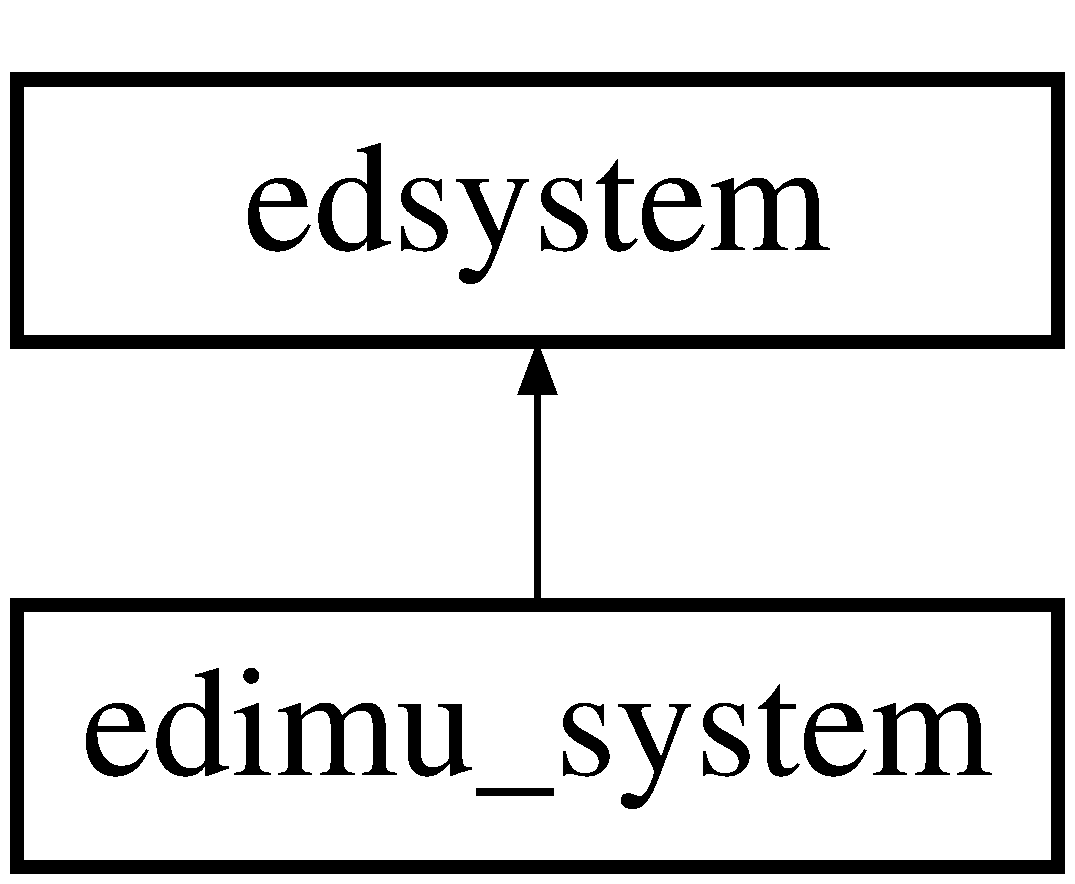
\includegraphics[height=2.000000cm]{classedimu__system}
\end{center}
\end{figure}
\subsection*{Public Types}
\begin{DoxyCompactItemize}
\item 
enum \hyperlink{classedimu__system_ac676a08f02fdc00d8e8210985f03e692}{g\-\_\-scale} \{ \hyperlink{classedimu__system_ac676a08f02fdc00d8e8210985f03e692ae3ca8f1426d51135044acb876bbf8d62}{G\-\_\-\-S\-C\-A\-L\-E\-\_\-245\-D\-P\-S}, 
\hyperlink{classedimu__system_ac676a08f02fdc00d8e8210985f03e692ac75709ac7d6a83a5c8fa75d61a550cdd}{G\-\_\-\-S\-C\-A\-L\-E\-\_\-500\-D\-P\-S}, 
\hyperlink{classedimu__system_ac676a08f02fdc00d8e8210985f03e692aee32250020a13cdce09a11247d4dec46}{G\-\_\-\-S\-C\-A\-L\-E\-\_\-2000\-D\-P\-S}
 \}
\begin{DoxyCompactList}\small\item\em possible ranges of the gyroscope \end{DoxyCompactList}\item 
enum \hyperlink{classedimu__system_a61602a34b68df60f8f10c1cd7af37707}{a\-\_\-scale} \{ \\*
\hyperlink{classedimu__system_a61602a34b68df60f8f10c1cd7af37707aad79008dcf3400051f927a49d8ea079b}{A\-\_\-\-S\-C\-A\-L\-E\-\_\-2\-G}, 
\hyperlink{classedimu__system_a61602a34b68df60f8f10c1cd7af37707a266db1462a0f522e112882219edde397}{A\-\_\-\-S\-C\-A\-L\-E\-\_\-4\-G}, 
\hyperlink{classedimu__system_a61602a34b68df60f8f10c1cd7af37707a1b2236322d581b3b4ec808b5c754b95c}{A\-\_\-\-S\-C\-A\-L\-E\-\_\-6\-G}, 
\hyperlink{classedimu__system_a61602a34b68df60f8f10c1cd7af37707a9db696dbf82ab98ea5645e1277a1cb50}{A\-\_\-\-S\-C\-A\-L\-E\-\_\-8\-G}, 
\\*
\hyperlink{classedimu__system_a61602a34b68df60f8f10c1cd7af37707ac36f1eb434af93d54110b82882463ae0}{A\-\_\-\-S\-C\-A\-L\-E\-\_\-16\-G}
 \}
\begin{DoxyCompactList}\small\item\em Possible F\-S\-R's of the accelerometer. \end{DoxyCompactList}\item 
enum \hyperlink{classedimu__system_ae7dbbcd66d0e16d693ac560884871da3}{m\-\_\-scale} \{ \hyperlink{classedimu__system_ae7dbbcd66d0e16d693ac560884871da3a1e2b05cb9c5203ecf8de8f02274aa875}{M\-\_\-\-S\-C\-A\-L\-E\-\_\-2\-G\-S}, 
\hyperlink{classedimu__system_ae7dbbcd66d0e16d693ac560884871da3af5c9b84c56a16b30a438ce2cd0a80d60}{M\-\_\-\-S\-C\-A\-L\-E\-\_\-4\-G\-S}, 
\hyperlink{classedimu__system_ae7dbbcd66d0e16d693ac560884871da3ad7d18ad9a5cc8188c90ead4a1b3c9dc5}{M\-\_\-\-S\-C\-A\-L\-E\-\_\-8\-G\-S}, 
\hyperlink{classedimu__system_ae7dbbcd66d0e16d693ac560884871da3ab26ba594363c13a86809357673513d33}{M\-\_\-\-S\-C\-A\-L\-E\-\_\-12\-G\-S}
 \}
\begin{DoxyCompactList}\small\item\em Possible F\-S\-R's of the magnetometer. \end{DoxyCompactList}\item 
enum \hyperlink{classedimu__system_aa3293bf451856110ad0b082b9ec0f857}{g\-\_\-odr} \{ \\*
\hyperlink{classedimu__system_aa3293bf451856110ad0b082b9ec0f857a7d3f6e71791376f2d1b2d2c81807ebb3}{G\-\_\-\-O\-D\-R\-\_\-95\-\_\-\-B\-W\-\_\-125} = 0x0, 
\hyperlink{classedimu__system_aa3293bf451856110ad0b082b9ec0f857a5d2fc14a0048ca8eab15315e03d0b7f6}{G\-\_\-\-O\-D\-R\-\_\-95\-\_\-\-B\-W\-\_\-25} = 0x1, 
\hyperlink{classedimu__system_aa3293bf451856110ad0b082b9ec0f857a8c12ef2286ffa75355d5061da725c320}{G\-\_\-\-O\-D\-R\-\_\-190\-\_\-\-B\-W\-\_\-125} = 0x4, 
\hyperlink{classedimu__system_aa3293bf451856110ad0b082b9ec0f857a986d076cfaa392fa58508b98a397a872}{G\-\_\-\-O\-D\-R\-\_\-190\-\_\-\-B\-W\-\_\-25} = 0x5, 
\\*
\hyperlink{classedimu__system_aa3293bf451856110ad0b082b9ec0f857ae0dee541e707db36687a7ad3fcb85acc}{G\-\_\-\-O\-D\-R\-\_\-190\-\_\-\-B\-W\-\_\-50} = 0x6, 
\hyperlink{classedimu__system_aa3293bf451856110ad0b082b9ec0f857a66466db4312dadf3b3f38b0abf01b448}{G\-\_\-\-O\-D\-R\-\_\-190\-\_\-\-B\-W\-\_\-70} = 0x7, 
\hyperlink{classedimu__system_aa3293bf451856110ad0b082b9ec0f857afb3501066d4ab609261676771bb47852}{G\-\_\-\-O\-D\-R\-\_\-380\-\_\-\-B\-W\-\_\-20} = 0x8, 
\hyperlink{classedimu__system_aa3293bf451856110ad0b082b9ec0f857a04d047c632a24ae7cd0e85575fd2a83b}{G\-\_\-\-O\-D\-R\-\_\-380\-\_\-\-B\-W\-\_\-25} = 0x9, 
\\*
\hyperlink{classedimu__system_aa3293bf451856110ad0b082b9ec0f857a92acbaa3992716666e3d34a9127e11e3}{G\-\_\-\-O\-D\-R\-\_\-380\-\_\-\-B\-W\-\_\-50} = 0x\-A, 
\hyperlink{classedimu__system_aa3293bf451856110ad0b082b9ec0f857a2fa626b536fce0640868fa5b32884ba1}{G\-\_\-\-O\-D\-R\-\_\-380\-\_\-\-B\-W\-\_\-100} = 0x\-B, 
\hyperlink{classedimu__system_aa3293bf451856110ad0b082b9ec0f857a3604bd7462bdbe0bdb2c7c6ea3ed439a}{G\-\_\-\-O\-D\-R\-\_\-760\-\_\-\-B\-W\-\_\-30} = 0x\-C, 
\hyperlink{classedimu__system_aa3293bf451856110ad0b082b9ec0f857a6eb0a12445b6fa37d4f889b1f2753dd4}{G\-\_\-\-O\-D\-R\-\_\-760\-\_\-\-B\-W\-\_\-35} = 0x\-D, 
\\*
\hyperlink{classedimu__system_aa3293bf451856110ad0b082b9ec0f857ab0c158480ed9b5a6755d2a33d7d6d6ed}{G\-\_\-\-O\-D\-R\-\_\-760\-\_\-\-B\-W\-\_\-50} = 0x\-E, 
\hyperlink{classedimu__system_aa3293bf451856110ad0b082b9ec0f857aee29786b1e5a4f06a9d3f83bc0a94f45}{G\-\_\-\-O\-D\-R\-\_\-760\-\_\-\-B\-W\-\_\-100} = 0x\-F
 \}
\begin{DoxyCompactList}\small\item\em Possible data rate/bandwidth combos of the gyro. \end{DoxyCompactList}\item 
enum \hyperlink{classedimu__system_a4950d1ca91416ce2221f9f251a4ab409}{a\-\_\-odr} \{ \\*
\hyperlink{classedimu__system_a4950d1ca91416ce2221f9f251a4ab409a612669c7c2e709c2599c8f1205fc6789}{A\-\_\-\-P\-O\-W\-E\-R\-\_\-\-D\-O\-W\-N}, 
\hyperlink{classedimu__system_a4950d1ca91416ce2221f9f251a4ab409a985e1725f4d2b592addd3ce39c6b9d67}{A\-\_\-\-O\-D\-R\-\_\-3125}, 
\hyperlink{classedimu__system_a4950d1ca91416ce2221f9f251a4ab409a39562621cfa654b48c8fb1e7d6547ea1}{A\-\_\-\-O\-D\-R\-\_\-625}, 
\hyperlink{classedimu__system_a4950d1ca91416ce2221f9f251a4ab409a3c446dbff5f9525174ec1babedd00130}{A\-\_\-\-O\-D\-R\-\_\-125}, 
\\*
\hyperlink{classedimu__system_a4950d1ca91416ce2221f9f251a4ab409a1c556e092ac518da584bf7ae59d8169d}{A\-\_\-\-O\-D\-R\-\_\-25}, 
\hyperlink{classedimu__system_a4950d1ca91416ce2221f9f251a4ab409adaeb950e8705c779eefbde7c4a05a6d4}{A\-\_\-\-O\-D\-R\-\_\-50}, 
\hyperlink{classedimu__system_a4950d1ca91416ce2221f9f251a4ab409ac5c6a9f89b38b88c58d72f828a9489d7}{A\-\_\-\-O\-D\-R\-\_\-100}, 
\hyperlink{classedimu__system_a4950d1ca91416ce2221f9f251a4ab409a8a602041d9319a516e9a70d7ebe464b4}{A\-\_\-\-O\-D\-R\-\_\-200}, 
\\*
\hyperlink{classedimu__system_a4950d1ca91416ce2221f9f251a4ab409a2e581fcaddb09bada44ee82120dc720f}{A\-\_\-\-O\-D\-R\-\_\-400}, 
\hyperlink{classedimu__system_a4950d1ca91416ce2221f9f251a4ab409ac08490b692283f696f7725ca348037e6}{A\-\_\-\-O\-D\-R\-\_\-800}, 
\hyperlink{classedimu__system_a4950d1ca91416ce2221f9f251a4ab409a2505e8202c185b7a0fd9d3a2c84506e6}{A\-\_\-\-O\-D\-R\-\_\-1600}
 \}
\begin{DoxyCompactList}\small\item\em Possible output data rates of the accelerometer. \end{DoxyCompactList}\item 
enum \hyperlink{classedimu__system_a94b2ea4b980c77a0156baae05fafa278}{a\-\_\-abw} \{ \hyperlink{classedimu__system_a94b2ea4b980c77a0156baae05fafa278a673459ef7230a157b1c9133682e5ef38}{A\-\_\-\-A\-B\-W\-\_\-773}, 
\hyperlink{classedimu__system_a94b2ea4b980c77a0156baae05fafa278abebf3506c669b49e8bb0e9b336a11836}{A\-\_\-\-A\-B\-W\-\_\-194}, 
\hyperlink{classedimu__system_a94b2ea4b980c77a0156baae05fafa278ab3ac328f4e427ce2c7d9dc67243b4446}{A\-\_\-\-A\-B\-W\-\_\-362}, 
\hyperlink{classedimu__system_a94b2ea4b980c77a0156baae05fafa278af6a4898c64003bfa125ce107f06ba1fe}{A\-\_\-\-A\-B\-W\-\_\-50}
 \}
\begin{DoxyCompactList}\small\item\em Possible anti-\/aliasing filter rates of the accelerometer. \end{DoxyCompactList}\item 
enum \hyperlink{classedimu__system_a6912f3ae02645ead8e47b96ebf275b7c}{m\-\_\-odr} \{ \\*
\hyperlink{classedimu__system_a6912f3ae02645ead8e47b96ebf275b7cafe1b71a13c2a85d99faa46ba295b0036}{M\-\_\-\-O\-D\-R\-\_\-3125}, 
\hyperlink{classedimu__system_a6912f3ae02645ead8e47b96ebf275b7ca5e23f8438b6c448bb3e857de0e6652fd}{M\-\_\-\-O\-D\-R\-\_\-625}, 
\hyperlink{classedimu__system_a6912f3ae02645ead8e47b96ebf275b7cadc5ab3742496b399082a63ca1b7be3b2}{M\-\_\-\-O\-D\-R\-\_\-125}, 
\hyperlink{classedimu__system_a6912f3ae02645ead8e47b96ebf275b7ca625f92a758b2591f1fa1bf7e00c8a492}{M\-\_\-\-O\-D\-R\-\_\-25}, 
\\*
\hyperlink{classedimu__system_a6912f3ae02645ead8e47b96ebf275b7ca0ea0e32be6c9cd0a7813aec7116d978b}{M\-\_\-\-O\-D\-R\-\_\-50}, 
\hyperlink{classedimu__system_a6912f3ae02645ead8e47b96ebf275b7caa678e4ce37cb70e5b4d06e63dc4226a6}{M\-\_\-\-O\-D\-R\-\_\-100}
 \}
\begin{DoxyCompactList}\small\item\em Possible output data rates of the magnetometer. \end{DoxyCompactList}\end{DoxyCompactItemize}
\subsection*{Public Member Functions}
\begin{DoxyCompactItemize}
\item 
\hyperlink{classedimu__system_a4c17647ced26f28a162520da42f32d13}{edimu\-\_\-system} ()
\item 
\hyperlink{classedimu__system_a382054be9280e8c43e4bc93a05a610c3}{$\sim$edimu\-\_\-system} ()
\item 
\hyperlink{classedimu__system_a94b2ea4b980c77a0156baae05fafa278}{a\-\_\-abw} \hyperlink{classedimu__system_adcec29ff9303db25800cf8026e0c6b37}{accel\-\_\-aa} ()
\item 
\hyperlink{classedimu__system_a61602a34b68df60f8f10c1cd7af37707}{a\-\_\-scale} \hyperlink{classedimu__system_a16ad8b9dbb9a889c2191de9774377882}{accel\-\_\-scale} ()
\item 
\hyperlink{classedimu__system_a4950d1ca91416ce2221f9f251a4ab409}{a\-\_\-odr} \hyperlink{classedimu__system_a5e7fbd97fe33973ec60c1e180b19b797}{accel\-\_\-datarate} ()
\item 
void \hyperlink{classedimu__system_a9ee88f6e0ae602d0037c2f7b0d43f3f8}{calibrate} ()
\item 
\hyperlink{classedimu__system_ac676a08f02fdc00d8e8210985f03e692}{g\-\_\-scale} \hyperlink{classedimu__system_a4f625e2eecfc7a0bb14c7a6195c82771}{gyro\-\_\-scale} ()
\item 
\hyperlink{classedimu__system_aa3293bf451856110ad0b082b9ec0f857}{g\-\_\-odr} \hyperlink{classedimu__system_a2bbaffa196674d42427bc4da6ac8164e}{gyro\-\_\-datarate} ()
\item 
\hyperlink{classedimu__system_ae7dbbcd66d0e16d693ac560884871da3}{m\-\_\-scale} \hyperlink{classedimu__system_ad21c665f25ae14f1da2d46e4274ba6ae}{mag\-\_\-scale} ()
\item 
\hyperlink{classedimu__system_a6912f3ae02645ead8e47b96ebf275b7c}{m\-\_\-odr} \hyperlink{classedimu__system_addc80a5048d987161abd25187f0d449f}{mag\-\_\-datarate} ()
\item 
void \hyperlink{classedimu__system_af745d305e5ff1cfaba3134fd4ff2c342}{init} ()
\item 
bool \hyperlink{classedimu__system_abd6e59b943adbb48fa786f10f809070c}{process} (\hyperlink{structedmessage}{edmessage} $\ast$msg)
\item 
void \hyperlink{classedimu__system_a65927db96dc88e8752f0529d9faa6bc0}{release} ()
\item 
void \hyperlink{classedimu__system_ad77a172b80472604b958abe1a7b037a0}{set\-\_\-accel\-\_\-aa} (\hyperlink{classedimu__system_a94b2ea4b980c77a0156baae05fafa278}{a\-\_\-abw} antialiasing)
\item 
void \hyperlink{classedimu__system_a1bed4d35a4ddc0590694a805fffa7c9f}{set\-\_\-accel\-\_\-scale} (\hyperlink{classedimu__system_a61602a34b68df60f8f10c1cd7af37707}{a\-\_\-scale} scale)
\item 
void \hyperlink{classedimu__system_ab813efe0e33b7e6f70af8d6b390a0076}{set\-\_\-accel\-\_\-datarate} (\hyperlink{classedimu__system_a4950d1ca91416ce2221f9f251a4ab409}{a\-\_\-odr} datarate)
\item 
void \hyperlink{classedimu__system_ac765ce7726af6fba582035f5a24ce91e}{set\-\_\-gyro\-\_\-scale} (\hyperlink{classedimu__system_ac676a08f02fdc00d8e8210985f03e692}{g\-\_\-scale} scale)
\item 
void \hyperlink{classedimu__system_a5c188e537c342e56a10d70c8c1a4f9bc}{set\-\_\-gyro\-\_\-datarate} (\hyperlink{classedimu__system_aa3293bf451856110ad0b082b9ec0f857}{g\-\_\-odr} datarate)
\item 
void \hyperlink{classedimu__system_a930fac9420df70417b040d554e29d8db}{set\-\_\-mag\-\_\-scale} (\hyperlink{classedimu__system_ae7dbbcd66d0e16d693ac560884871da3}{m\-\_\-scale} scale)
\item 
void \hyperlink{classedimu__system_aa773e0db8441dc11bbb8399dede49a9c}{set\-\_\-mag\-\_\-datarate} (\hyperlink{classedimu__system_a6912f3ae02645ead8e47b96ebf275b7c}{m\-\_\-odr} datarate)
\item 
void \hyperlink{classedimu__system_a70926a3b36b53f54913fc47ee471fb9b}{update} ()
\item 
std\-::string \hyperlink{classedimu__system_ae3124c577ae10d92f69438f28ce67969}{typestr} ()
\end{DoxyCompactItemize}
\subsection*{Static Public Member Functions}
\begin{DoxyCompactItemize}
\item 
static std\-::string \hyperlink{classedimu__system_a850c2b8420aef618edf9ec36f9436ed4}{Type\-String} ()
\end{DoxyCompactItemize}


\subsection{Member Enumeration Documentation}
\hypertarget{classedimu__system_a94b2ea4b980c77a0156baae05fafa278}{\index{edimu\-\_\-system@{edimu\-\_\-system}!a\-\_\-abw@{a\-\_\-abw}}
\index{a\-\_\-abw@{a\-\_\-abw}!edimu_system@{edimu\-\_\-system}}
\subsubsection[{a\-\_\-abw}]{\setlength{\rightskip}{0pt plus 5cm}enum {\bf edimu\-\_\-system\-::a\-\_\-abw}}}\label{classedimu__system_a94b2ea4b980c77a0156baae05fafa278}


Possible anti-\/aliasing filter rates of the accelerometer. 

\begin{Desc}
\item[Enumerator]\par
\begin{description}
\index{A\-\_\-\-A\-B\-W\-\_\-773@{A\-\_\-\-A\-B\-W\-\_\-773}!edimu\-\_\-system@{edimu\-\_\-system}}\index{edimu\-\_\-system@{edimu\-\_\-system}!A\-\_\-\-A\-B\-W\-\_\-773@{A\-\_\-\-A\-B\-W\-\_\-773}}\item[{\em 
\hypertarget{classedimu__system_a94b2ea4b980c77a0156baae05fafa278a673459ef7230a157b1c9133682e5ef38}{A\-\_\-\-A\-B\-W\-\_\-773}\label{classedimu__system_a94b2ea4b980c77a0156baae05fafa278a673459ef7230a157b1c9133682e5ef38}
}]773 Hz (0x0) \index{A\-\_\-\-A\-B\-W\-\_\-194@{A\-\_\-\-A\-B\-W\-\_\-194}!edimu\-\_\-system@{edimu\-\_\-system}}\index{edimu\-\_\-system@{edimu\-\_\-system}!A\-\_\-\-A\-B\-W\-\_\-194@{A\-\_\-\-A\-B\-W\-\_\-194}}\item[{\em 
\hypertarget{classedimu__system_a94b2ea4b980c77a0156baae05fafa278abebf3506c669b49e8bb0e9b336a11836}{A\-\_\-\-A\-B\-W\-\_\-194}\label{classedimu__system_a94b2ea4b980c77a0156baae05fafa278abebf3506c669b49e8bb0e9b336a11836}
}]194 Hz (0x1) \index{A\-\_\-\-A\-B\-W\-\_\-362@{A\-\_\-\-A\-B\-W\-\_\-362}!edimu\-\_\-system@{edimu\-\_\-system}}\index{edimu\-\_\-system@{edimu\-\_\-system}!A\-\_\-\-A\-B\-W\-\_\-362@{A\-\_\-\-A\-B\-W\-\_\-362}}\item[{\em 
\hypertarget{classedimu__system_a94b2ea4b980c77a0156baae05fafa278ab3ac328f4e427ce2c7d9dc67243b4446}{A\-\_\-\-A\-B\-W\-\_\-362}\label{classedimu__system_a94b2ea4b980c77a0156baae05fafa278ab3ac328f4e427ce2c7d9dc67243b4446}
}]362 Hz (0x2) \index{A\-\_\-\-A\-B\-W\-\_\-50@{A\-\_\-\-A\-B\-W\-\_\-50}!edimu\-\_\-system@{edimu\-\_\-system}}\index{edimu\-\_\-system@{edimu\-\_\-system}!A\-\_\-\-A\-B\-W\-\_\-50@{A\-\_\-\-A\-B\-W\-\_\-50}}\item[{\em 
\hypertarget{classedimu__system_a94b2ea4b980c77a0156baae05fafa278af6a4898c64003bfa125ce107f06ba1fe}{A\-\_\-\-A\-B\-W\-\_\-50}\label{classedimu__system_a94b2ea4b980c77a0156baae05fafa278af6a4898c64003bfa125ce107f06ba1fe}
}]50 Hz (0x3) \end{description}
\end{Desc}
\hypertarget{classedimu__system_a4950d1ca91416ce2221f9f251a4ab409}{\index{edimu\-\_\-system@{edimu\-\_\-system}!a\-\_\-odr@{a\-\_\-odr}}
\index{a\-\_\-odr@{a\-\_\-odr}!edimu_system@{edimu\-\_\-system}}
\subsubsection[{a\-\_\-odr}]{\setlength{\rightskip}{0pt plus 5cm}enum {\bf edimu\-\_\-system\-::a\-\_\-odr}}}\label{classedimu__system_a4950d1ca91416ce2221f9f251a4ab409}


Possible output data rates of the accelerometer. 

\begin{Desc}
\item[Enumerator]\par
\begin{description}
\index{A\-\_\-\-P\-O\-W\-E\-R\-\_\-\-D\-O\-W\-N@{A\-\_\-\-P\-O\-W\-E\-R\-\_\-\-D\-O\-W\-N}!edimu\-\_\-system@{edimu\-\_\-system}}\index{edimu\-\_\-system@{edimu\-\_\-system}!A\-\_\-\-P\-O\-W\-E\-R\-\_\-\-D\-O\-W\-N@{A\-\_\-\-P\-O\-W\-E\-R\-\_\-\-D\-O\-W\-N}}\item[{\em 
\hypertarget{classedimu__system_a4950d1ca91416ce2221f9f251a4ab409a612669c7c2e709c2599c8f1205fc6789}{A\-\_\-\-P\-O\-W\-E\-R\-\_\-\-D\-O\-W\-N}\label{classedimu__system_a4950d1ca91416ce2221f9f251a4ab409a612669c7c2e709c2599c8f1205fc6789}
}]Power-\/down mode (0x0) \index{A\-\_\-\-O\-D\-R\-\_\-3125@{A\-\_\-\-O\-D\-R\-\_\-3125}!edimu\-\_\-system@{edimu\-\_\-system}}\index{edimu\-\_\-system@{edimu\-\_\-system}!A\-\_\-\-O\-D\-R\-\_\-3125@{A\-\_\-\-O\-D\-R\-\_\-3125}}\item[{\em 
\hypertarget{classedimu__system_a4950d1ca91416ce2221f9f251a4ab409a985e1725f4d2b592addd3ce39c6b9d67}{A\-\_\-\-O\-D\-R\-\_\-3125}\label{classedimu__system_a4950d1ca91416ce2221f9f251a4ab409a985e1725f4d2b592addd3ce39c6b9d67}
}]3.\-125 Hz (0x1) \index{A\-\_\-\-O\-D\-R\-\_\-625@{A\-\_\-\-O\-D\-R\-\_\-625}!edimu\-\_\-system@{edimu\-\_\-system}}\index{edimu\-\_\-system@{edimu\-\_\-system}!A\-\_\-\-O\-D\-R\-\_\-625@{A\-\_\-\-O\-D\-R\-\_\-625}}\item[{\em 
\hypertarget{classedimu__system_a4950d1ca91416ce2221f9f251a4ab409a39562621cfa654b48c8fb1e7d6547ea1}{A\-\_\-\-O\-D\-R\-\_\-625}\label{classedimu__system_a4950d1ca91416ce2221f9f251a4ab409a39562621cfa654b48c8fb1e7d6547ea1}
}]6.\-25 Hz (0x2) \index{A\-\_\-\-O\-D\-R\-\_\-125@{A\-\_\-\-O\-D\-R\-\_\-125}!edimu\-\_\-system@{edimu\-\_\-system}}\index{edimu\-\_\-system@{edimu\-\_\-system}!A\-\_\-\-O\-D\-R\-\_\-125@{A\-\_\-\-O\-D\-R\-\_\-125}}\item[{\em 
\hypertarget{classedimu__system_a4950d1ca91416ce2221f9f251a4ab409a3c446dbff5f9525174ec1babedd00130}{A\-\_\-\-O\-D\-R\-\_\-125}\label{classedimu__system_a4950d1ca91416ce2221f9f251a4ab409a3c446dbff5f9525174ec1babedd00130}
}]12.\-5 Hz (0x3) \index{A\-\_\-\-O\-D\-R\-\_\-25@{A\-\_\-\-O\-D\-R\-\_\-25}!edimu\-\_\-system@{edimu\-\_\-system}}\index{edimu\-\_\-system@{edimu\-\_\-system}!A\-\_\-\-O\-D\-R\-\_\-25@{A\-\_\-\-O\-D\-R\-\_\-25}}\item[{\em 
\hypertarget{classedimu__system_a4950d1ca91416ce2221f9f251a4ab409a1c556e092ac518da584bf7ae59d8169d}{A\-\_\-\-O\-D\-R\-\_\-25}\label{classedimu__system_a4950d1ca91416ce2221f9f251a4ab409a1c556e092ac518da584bf7ae59d8169d}
}]25 Hz (0x4) \index{A\-\_\-\-O\-D\-R\-\_\-50@{A\-\_\-\-O\-D\-R\-\_\-50}!edimu\-\_\-system@{edimu\-\_\-system}}\index{edimu\-\_\-system@{edimu\-\_\-system}!A\-\_\-\-O\-D\-R\-\_\-50@{A\-\_\-\-O\-D\-R\-\_\-50}}\item[{\em 
\hypertarget{classedimu__system_a4950d1ca91416ce2221f9f251a4ab409adaeb950e8705c779eefbde7c4a05a6d4}{A\-\_\-\-O\-D\-R\-\_\-50}\label{classedimu__system_a4950d1ca91416ce2221f9f251a4ab409adaeb950e8705c779eefbde7c4a05a6d4}
}]50 Hz (0x5) \index{A\-\_\-\-O\-D\-R\-\_\-100@{A\-\_\-\-O\-D\-R\-\_\-100}!edimu\-\_\-system@{edimu\-\_\-system}}\index{edimu\-\_\-system@{edimu\-\_\-system}!A\-\_\-\-O\-D\-R\-\_\-100@{A\-\_\-\-O\-D\-R\-\_\-100}}\item[{\em 
\hypertarget{classedimu__system_a4950d1ca91416ce2221f9f251a4ab409ac5c6a9f89b38b88c58d72f828a9489d7}{A\-\_\-\-O\-D\-R\-\_\-100}\label{classedimu__system_a4950d1ca91416ce2221f9f251a4ab409ac5c6a9f89b38b88c58d72f828a9489d7}
}]100 Hz (0x6) \index{A\-\_\-\-O\-D\-R\-\_\-200@{A\-\_\-\-O\-D\-R\-\_\-200}!edimu\-\_\-system@{edimu\-\_\-system}}\index{edimu\-\_\-system@{edimu\-\_\-system}!A\-\_\-\-O\-D\-R\-\_\-200@{A\-\_\-\-O\-D\-R\-\_\-200}}\item[{\em 
\hypertarget{classedimu__system_a4950d1ca91416ce2221f9f251a4ab409a8a602041d9319a516e9a70d7ebe464b4}{A\-\_\-\-O\-D\-R\-\_\-200}\label{classedimu__system_a4950d1ca91416ce2221f9f251a4ab409a8a602041d9319a516e9a70d7ebe464b4}
}]200 Hz (0x7) \index{A\-\_\-\-O\-D\-R\-\_\-400@{A\-\_\-\-O\-D\-R\-\_\-400}!edimu\-\_\-system@{edimu\-\_\-system}}\index{edimu\-\_\-system@{edimu\-\_\-system}!A\-\_\-\-O\-D\-R\-\_\-400@{A\-\_\-\-O\-D\-R\-\_\-400}}\item[{\em 
\hypertarget{classedimu__system_a4950d1ca91416ce2221f9f251a4ab409a2e581fcaddb09bada44ee82120dc720f}{A\-\_\-\-O\-D\-R\-\_\-400}\label{classedimu__system_a4950d1ca91416ce2221f9f251a4ab409a2e581fcaddb09bada44ee82120dc720f}
}]400 Hz (0x8) \index{A\-\_\-\-O\-D\-R\-\_\-800@{A\-\_\-\-O\-D\-R\-\_\-800}!edimu\-\_\-system@{edimu\-\_\-system}}\index{edimu\-\_\-system@{edimu\-\_\-system}!A\-\_\-\-O\-D\-R\-\_\-800@{A\-\_\-\-O\-D\-R\-\_\-800}}\item[{\em 
\hypertarget{classedimu__system_a4950d1ca91416ce2221f9f251a4ab409ac08490b692283f696f7725ca348037e6}{A\-\_\-\-O\-D\-R\-\_\-800}\label{classedimu__system_a4950d1ca91416ce2221f9f251a4ab409ac08490b692283f696f7725ca348037e6}
}]800 Hz (9) \index{A\-\_\-\-O\-D\-R\-\_\-1600@{A\-\_\-\-O\-D\-R\-\_\-1600}!edimu\-\_\-system@{edimu\-\_\-system}}\index{edimu\-\_\-system@{edimu\-\_\-system}!A\-\_\-\-O\-D\-R\-\_\-1600@{A\-\_\-\-O\-D\-R\-\_\-1600}}\item[{\em 
\hypertarget{classedimu__system_a4950d1ca91416ce2221f9f251a4ab409a2505e8202c185b7a0fd9d3a2c84506e6}{A\-\_\-\-O\-D\-R\-\_\-1600}\label{classedimu__system_a4950d1ca91416ce2221f9f251a4ab409a2505e8202c185b7a0fd9d3a2c84506e6}
}]1600 Hz (0x\-A) \end{description}
\end{Desc}
\hypertarget{classedimu__system_a61602a34b68df60f8f10c1cd7af37707}{\index{edimu\-\_\-system@{edimu\-\_\-system}!a\-\_\-scale@{a\-\_\-scale}}
\index{a\-\_\-scale@{a\-\_\-scale}!edimu_system@{edimu\-\_\-system}}
\subsubsection[{a\-\_\-scale}]{\setlength{\rightskip}{0pt plus 5cm}enum {\bf edimu\-\_\-system\-::a\-\_\-scale}}}\label{classedimu__system_a61602a34b68df60f8f10c1cd7af37707}


Possible F\-S\-R's of the accelerometer. 

\begin{Desc}
\item[Enumerator]\par
\begin{description}
\index{A\-\_\-\-S\-C\-A\-L\-E\-\_\-2\-G@{A\-\_\-\-S\-C\-A\-L\-E\-\_\-2\-G}!edimu\-\_\-system@{edimu\-\_\-system}}\index{edimu\-\_\-system@{edimu\-\_\-system}!A\-\_\-\-S\-C\-A\-L\-E\-\_\-2\-G@{A\-\_\-\-S\-C\-A\-L\-E\-\_\-2\-G}}\item[{\em 
\hypertarget{classedimu__system_a61602a34b68df60f8f10c1cd7af37707aad79008dcf3400051f927a49d8ea079b}{A\-\_\-\-S\-C\-A\-L\-E\-\_\-2\-G}\label{classedimu__system_a61602a34b68df60f8f10c1cd7af37707aad79008dcf3400051f927a49d8ea079b}
}]2g \index{A\-\_\-\-S\-C\-A\-L\-E\-\_\-4\-G@{A\-\_\-\-S\-C\-A\-L\-E\-\_\-4\-G}!edimu\-\_\-system@{edimu\-\_\-system}}\index{edimu\-\_\-system@{edimu\-\_\-system}!A\-\_\-\-S\-C\-A\-L\-E\-\_\-4\-G@{A\-\_\-\-S\-C\-A\-L\-E\-\_\-4\-G}}\item[{\em 
\hypertarget{classedimu__system_a61602a34b68df60f8f10c1cd7af37707a266db1462a0f522e112882219edde397}{A\-\_\-\-S\-C\-A\-L\-E\-\_\-4\-G}\label{classedimu__system_a61602a34b68df60f8f10c1cd7af37707a266db1462a0f522e112882219edde397}
}]4g \index{A\-\_\-\-S\-C\-A\-L\-E\-\_\-6\-G@{A\-\_\-\-S\-C\-A\-L\-E\-\_\-6\-G}!edimu\-\_\-system@{edimu\-\_\-system}}\index{edimu\-\_\-system@{edimu\-\_\-system}!A\-\_\-\-S\-C\-A\-L\-E\-\_\-6\-G@{A\-\_\-\-S\-C\-A\-L\-E\-\_\-6\-G}}\item[{\em 
\hypertarget{classedimu__system_a61602a34b68df60f8f10c1cd7af37707a1b2236322d581b3b4ec808b5c754b95c}{A\-\_\-\-S\-C\-A\-L\-E\-\_\-6\-G}\label{classedimu__system_a61602a34b68df60f8f10c1cd7af37707a1b2236322d581b3b4ec808b5c754b95c}
}]6g \index{A\-\_\-\-S\-C\-A\-L\-E\-\_\-8\-G@{A\-\_\-\-S\-C\-A\-L\-E\-\_\-8\-G}!edimu\-\_\-system@{edimu\-\_\-system}}\index{edimu\-\_\-system@{edimu\-\_\-system}!A\-\_\-\-S\-C\-A\-L\-E\-\_\-8\-G@{A\-\_\-\-S\-C\-A\-L\-E\-\_\-8\-G}}\item[{\em 
\hypertarget{classedimu__system_a61602a34b68df60f8f10c1cd7af37707a9db696dbf82ab98ea5645e1277a1cb50}{A\-\_\-\-S\-C\-A\-L\-E\-\_\-8\-G}\label{classedimu__system_a61602a34b68df60f8f10c1cd7af37707a9db696dbf82ab98ea5645e1277a1cb50}
}]8g \index{A\-\_\-\-S\-C\-A\-L\-E\-\_\-16\-G@{A\-\_\-\-S\-C\-A\-L\-E\-\_\-16\-G}!edimu\-\_\-system@{edimu\-\_\-system}}\index{edimu\-\_\-system@{edimu\-\_\-system}!A\-\_\-\-S\-C\-A\-L\-E\-\_\-16\-G@{A\-\_\-\-S\-C\-A\-L\-E\-\_\-16\-G}}\item[{\em 
\hypertarget{classedimu__system_a61602a34b68df60f8f10c1cd7af37707ac36f1eb434af93d54110b82882463ae0}{A\-\_\-\-S\-C\-A\-L\-E\-\_\-16\-G}\label{classedimu__system_a61602a34b68df60f8f10c1cd7af37707ac36f1eb434af93d54110b82882463ae0}
}]16g \end{description}
\end{Desc}
\hypertarget{classedimu__system_aa3293bf451856110ad0b082b9ec0f857}{\index{edimu\-\_\-system@{edimu\-\_\-system}!g\-\_\-odr@{g\-\_\-odr}}
\index{g\-\_\-odr@{g\-\_\-odr}!edimu_system@{edimu\-\_\-system}}
\subsubsection[{g\-\_\-odr}]{\setlength{\rightskip}{0pt plus 5cm}enum {\bf edimu\-\_\-system\-::g\-\_\-odr}}}\label{classedimu__system_aa3293bf451856110ad0b082b9ec0f857}


Possible data rate/bandwidth combos of the gyro. 

\begin{Desc}
\item[Enumerator]\par
\begin{description}
\index{G\-\_\-\-O\-D\-R\-\_\-95\-\_\-\-B\-W\-\_\-125@{G\-\_\-\-O\-D\-R\-\_\-95\-\_\-\-B\-W\-\_\-125}!edimu\-\_\-system@{edimu\-\_\-system}}\index{edimu\-\_\-system@{edimu\-\_\-system}!G\-\_\-\-O\-D\-R\-\_\-95\-\_\-\-B\-W\-\_\-125@{G\-\_\-\-O\-D\-R\-\_\-95\-\_\-\-B\-W\-\_\-125}}\item[{\em 
\hypertarget{classedimu__system_aa3293bf451856110ad0b082b9ec0f857a7d3f6e71791376f2d1b2d2c81807ebb3}{G\-\_\-\-O\-D\-R\-\_\-95\-\_\-\-B\-W\-\_\-125}\label{classedimu__system_aa3293bf451856110ad0b082b9ec0f857a7d3f6e71791376f2d1b2d2c81807ebb3}
}]95 12.\-5 \index{G\-\_\-\-O\-D\-R\-\_\-95\-\_\-\-B\-W\-\_\-25@{G\-\_\-\-O\-D\-R\-\_\-95\-\_\-\-B\-W\-\_\-25}!edimu\-\_\-system@{edimu\-\_\-system}}\index{edimu\-\_\-system@{edimu\-\_\-system}!G\-\_\-\-O\-D\-R\-\_\-95\-\_\-\-B\-W\-\_\-25@{G\-\_\-\-O\-D\-R\-\_\-95\-\_\-\-B\-W\-\_\-25}}\item[{\em 
\hypertarget{classedimu__system_aa3293bf451856110ad0b082b9ec0f857a5d2fc14a0048ca8eab15315e03d0b7f6}{G\-\_\-\-O\-D\-R\-\_\-95\-\_\-\-B\-W\-\_\-25}\label{classedimu__system_aa3293bf451856110ad0b082b9ec0f857a5d2fc14a0048ca8eab15315e03d0b7f6}
}]95 25 \index{G\-\_\-\-O\-D\-R\-\_\-190\-\_\-\-B\-W\-\_\-125@{G\-\_\-\-O\-D\-R\-\_\-190\-\_\-\-B\-W\-\_\-125}!edimu\-\_\-system@{edimu\-\_\-system}}\index{edimu\-\_\-system@{edimu\-\_\-system}!G\-\_\-\-O\-D\-R\-\_\-190\-\_\-\-B\-W\-\_\-125@{G\-\_\-\-O\-D\-R\-\_\-190\-\_\-\-B\-W\-\_\-125}}\item[{\em 
\hypertarget{classedimu__system_aa3293bf451856110ad0b082b9ec0f857a8c12ef2286ffa75355d5061da725c320}{G\-\_\-\-O\-D\-R\-\_\-190\-\_\-\-B\-W\-\_\-125}\label{classedimu__system_aa3293bf451856110ad0b082b9ec0f857a8c12ef2286ffa75355d5061da725c320}
}]190 12.\-5 \index{G\-\_\-\-O\-D\-R\-\_\-190\-\_\-\-B\-W\-\_\-25@{G\-\_\-\-O\-D\-R\-\_\-190\-\_\-\-B\-W\-\_\-25}!edimu\-\_\-system@{edimu\-\_\-system}}\index{edimu\-\_\-system@{edimu\-\_\-system}!G\-\_\-\-O\-D\-R\-\_\-190\-\_\-\-B\-W\-\_\-25@{G\-\_\-\-O\-D\-R\-\_\-190\-\_\-\-B\-W\-\_\-25}}\item[{\em 
\hypertarget{classedimu__system_aa3293bf451856110ad0b082b9ec0f857a986d076cfaa392fa58508b98a397a872}{G\-\_\-\-O\-D\-R\-\_\-190\-\_\-\-B\-W\-\_\-25}\label{classedimu__system_aa3293bf451856110ad0b082b9ec0f857a986d076cfaa392fa58508b98a397a872}
}]190 25 \index{G\-\_\-\-O\-D\-R\-\_\-190\-\_\-\-B\-W\-\_\-50@{G\-\_\-\-O\-D\-R\-\_\-190\-\_\-\-B\-W\-\_\-50}!edimu\-\_\-system@{edimu\-\_\-system}}\index{edimu\-\_\-system@{edimu\-\_\-system}!G\-\_\-\-O\-D\-R\-\_\-190\-\_\-\-B\-W\-\_\-50@{G\-\_\-\-O\-D\-R\-\_\-190\-\_\-\-B\-W\-\_\-50}}\item[{\em 
\hypertarget{classedimu__system_aa3293bf451856110ad0b082b9ec0f857ae0dee541e707db36687a7ad3fcb85acc}{G\-\_\-\-O\-D\-R\-\_\-190\-\_\-\-B\-W\-\_\-50}\label{classedimu__system_aa3293bf451856110ad0b082b9ec0f857ae0dee541e707db36687a7ad3fcb85acc}
}]190 50 \index{G\-\_\-\-O\-D\-R\-\_\-190\-\_\-\-B\-W\-\_\-70@{G\-\_\-\-O\-D\-R\-\_\-190\-\_\-\-B\-W\-\_\-70}!edimu\-\_\-system@{edimu\-\_\-system}}\index{edimu\-\_\-system@{edimu\-\_\-system}!G\-\_\-\-O\-D\-R\-\_\-190\-\_\-\-B\-W\-\_\-70@{G\-\_\-\-O\-D\-R\-\_\-190\-\_\-\-B\-W\-\_\-70}}\item[{\em 
\hypertarget{classedimu__system_aa3293bf451856110ad0b082b9ec0f857a66466db4312dadf3b3f38b0abf01b448}{G\-\_\-\-O\-D\-R\-\_\-190\-\_\-\-B\-W\-\_\-70}\label{classedimu__system_aa3293bf451856110ad0b082b9ec0f857a66466db4312dadf3b3f38b0abf01b448}
}]190 70 \index{G\-\_\-\-O\-D\-R\-\_\-380\-\_\-\-B\-W\-\_\-20@{G\-\_\-\-O\-D\-R\-\_\-380\-\_\-\-B\-W\-\_\-20}!edimu\-\_\-system@{edimu\-\_\-system}}\index{edimu\-\_\-system@{edimu\-\_\-system}!G\-\_\-\-O\-D\-R\-\_\-380\-\_\-\-B\-W\-\_\-20@{G\-\_\-\-O\-D\-R\-\_\-380\-\_\-\-B\-W\-\_\-20}}\item[{\em 
\hypertarget{classedimu__system_aa3293bf451856110ad0b082b9ec0f857afb3501066d4ab609261676771bb47852}{G\-\_\-\-O\-D\-R\-\_\-380\-\_\-\-B\-W\-\_\-20}\label{classedimu__system_aa3293bf451856110ad0b082b9ec0f857afb3501066d4ab609261676771bb47852}
}]380 20 \index{G\-\_\-\-O\-D\-R\-\_\-380\-\_\-\-B\-W\-\_\-25@{G\-\_\-\-O\-D\-R\-\_\-380\-\_\-\-B\-W\-\_\-25}!edimu\-\_\-system@{edimu\-\_\-system}}\index{edimu\-\_\-system@{edimu\-\_\-system}!G\-\_\-\-O\-D\-R\-\_\-380\-\_\-\-B\-W\-\_\-25@{G\-\_\-\-O\-D\-R\-\_\-380\-\_\-\-B\-W\-\_\-25}}\item[{\em 
\hypertarget{classedimu__system_aa3293bf451856110ad0b082b9ec0f857a04d047c632a24ae7cd0e85575fd2a83b}{G\-\_\-\-O\-D\-R\-\_\-380\-\_\-\-B\-W\-\_\-25}\label{classedimu__system_aa3293bf451856110ad0b082b9ec0f857a04d047c632a24ae7cd0e85575fd2a83b}
}]380 25 \index{G\-\_\-\-O\-D\-R\-\_\-380\-\_\-\-B\-W\-\_\-50@{G\-\_\-\-O\-D\-R\-\_\-380\-\_\-\-B\-W\-\_\-50}!edimu\-\_\-system@{edimu\-\_\-system}}\index{edimu\-\_\-system@{edimu\-\_\-system}!G\-\_\-\-O\-D\-R\-\_\-380\-\_\-\-B\-W\-\_\-50@{G\-\_\-\-O\-D\-R\-\_\-380\-\_\-\-B\-W\-\_\-50}}\item[{\em 
\hypertarget{classedimu__system_aa3293bf451856110ad0b082b9ec0f857a92acbaa3992716666e3d34a9127e11e3}{G\-\_\-\-O\-D\-R\-\_\-380\-\_\-\-B\-W\-\_\-50}\label{classedimu__system_aa3293bf451856110ad0b082b9ec0f857a92acbaa3992716666e3d34a9127e11e3}
}]380 50 \index{G\-\_\-\-O\-D\-R\-\_\-380\-\_\-\-B\-W\-\_\-100@{G\-\_\-\-O\-D\-R\-\_\-380\-\_\-\-B\-W\-\_\-100}!edimu\-\_\-system@{edimu\-\_\-system}}\index{edimu\-\_\-system@{edimu\-\_\-system}!G\-\_\-\-O\-D\-R\-\_\-380\-\_\-\-B\-W\-\_\-100@{G\-\_\-\-O\-D\-R\-\_\-380\-\_\-\-B\-W\-\_\-100}}\item[{\em 
\hypertarget{classedimu__system_aa3293bf451856110ad0b082b9ec0f857a2fa626b536fce0640868fa5b32884ba1}{G\-\_\-\-O\-D\-R\-\_\-380\-\_\-\-B\-W\-\_\-100}\label{classedimu__system_aa3293bf451856110ad0b082b9ec0f857a2fa626b536fce0640868fa5b32884ba1}
}]380 100 \index{G\-\_\-\-O\-D\-R\-\_\-760\-\_\-\-B\-W\-\_\-30@{G\-\_\-\-O\-D\-R\-\_\-760\-\_\-\-B\-W\-\_\-30}!edimu\-\_\-system@{edimu\-\_\-system}}\index{edimu\-\_\-system@{edimu\-\_\-system}!G\-\_\-\-O\-D\-R\-\_\-760\-\_\-\-B\-W\-\_\-30@{G\-\_\-\-O\-D\-R\-\_\-760\-\_\-\-B\-W\-\_\-30}}\item[{\em 
\hypertarget{classedimu__system_aa3293bf451856110ad0b082b9ec0f857a3604bd7462bdbe0bdb2c7c6ea3ed439a}{G\-\_\-\-O\-D\-R\-\_\-760\-\_\-\-B\-W\-\_\-30}\label{classedimu__system_aa3293bf451856110ad0b082b9ec0f857a3604bd7462bdbe0bdb2c7c6ea3ed439a}
}]760 30 \index{G\-\_\-\-O\-D\-R\-\_\-760\-\_\-\-B\-W\-\_\-35@{G\-\_\-\-O\-D\-R\-\_\-760\-\_\-\-B\-W\-\_\-35}!edimu\-\_\-system@{edimu\-\_\-system}}\index{edimu\-\_\-system@{edimu\-\_\-system}!G\-\_\-\-O\-D\-R\-\_\-760\-\_\-\-B\-W\-\_\-35@{G\-\_\-\-O\-D\-R\-\_\-760\-\_\-\-B\-W\-\_\-35}}\item[{\em 
\hypertarget{classedimu__system_aa3293bf451856110ad0b082b9ec0f857a6eb0a12445b6fa37d4f889b1f2753dd4}{G\-\_\-\-O\-D\-R\-\_\-760\-\_\-\-B\-W\-\_\-35}\label{classedimu__system_aa3293bf451856110ad0b082b9ec0f857a6eb0a12445b6fa37d4f889b1f2753dd4}
}]760 35 \index{G\-\_\-\-O\-D\-R\-\_\-760\-\_\-\-B\-W\-\_\-50@{G\-\_\-\-O\-D\-R\-\_\-760\-\_\-\-B\-W\-\_\-50}!edimu\-\_\-system@{edimu\-\_\-system}}\index{edimu\-\_\-system@{edimu\-\_\-system}!G\-\_\-\-O\-D\-R\-\_\-760\-\_\-\-B\-W\-\_\-50@{G\-\_\-\-O\-D\-R\-\_\-760\-\_\-\-B\-W\-\_\-50}}\item[{\em 
\hypertarget{classedimu__system_aa3293bf451856110ad0b082b9ec0f857ab0c158480ed9b5a6755d2a33d7d6d6ed}{G\-\_\-\-O\-D\-R\-\_\-760\-\_\-\-B\-W\-\_\-50}\label{classedimu__system_aa3293bf451856110ad0b082b9ec0f857ab0c158480ed9b5a6755d2a33d7d6d6ed}
}]760 50 \index{G\-\_\-\-O\-D\-R\-\_\-760\-\_\-\-B\-W\-\_\-100@{G\-\_\-\-O\-D\-R\-\_\-760\-\_\-\-B\-W\-\_\-100}!edimu\-\_\-system@{edimu\-\_\-system}}\index{edimu\-\_\-system@{edimu\-\_\-system}!G\-\_\-\-O\-D\-R\-\_\-760\-\_\-\-B\-W\-\_\-100@{G\-\_\-\-O\-D\-R\-\_\-760\-\_\-\-B\-W\-\_\-100}}\item[{\em 
\hypertarget{classedimu__system_aa3293bf451856110ad0b082b9ec0f857aee29786b1e5a4f06a9d3f83bc0a94f45}{G\-\_\-\-O\-D\-R\-\_\-760\-\_\-\-B\-W\-\_\-100}\label{classedimu__system_aa3293bf451856110ad0b082b9ec0f857aee29786b1e5a4f06a9d3f83bc0a94f45}
}]760 100 \end{description}
\end{Desc}
\hypertarget{classedimu__system_ac676a08f02fdc00d8e8210985f03e692}{\index{edimu\-\_\-system@{edimu\-\_\-system}!g\-\_\-scale@{g\-\_\-scale}}
\index{g\-\_\-scale@{g\-\_\-scale}!edimu_system@{edimu\-\_\-system}}
\subsubsection[{g\-\_\-scale}]{\setlength{\rightskip}{0pt plus 5cm}enum {\bf edimu\-\_\-system\-::g\-\_\-scale}}}\label{classedimu__system_ac676a08f02fdc00d8e8210985f03e692}


possible ranges of the gyroscope 

\begin{Desc}
\item[Enumerator]\par
\begin{description}
\index{G\-\_\-\-S\-C\-A\-L\-E\-\_\-245\-D\-P\-S@{G\-\_\-\-S\-C\-A\-L\-E\-\_\-245\-D\-P\-S}!edimu\-\_\-system@{edimu\-\_\-system}}\index{edimu\-\_\-system@{edimu\-\_\-system}!G\-\_\-\-S\-C\-A\-L\-E\-\_\-245\-D\-P\-S@{G\-\_\-\-S\-C\-A\-L\-E\-\_\-245\-D\-P\-S}}\item[{\em 
\hypertarget{classedimu__system_ac676a08f02fdc00d8e8210985f03e692ae3ca8f1426d51135044acb876bbf8d62}{G\-\_\-\-S\-C\-A\-L\-E\-\_\-245\-D\-P\-S}\label{classedimu__system_ac676a08f02fdc00d8e8210985f03e692ae3ca8f1426d51135044acb876bbf8d62}
}]245 degrees per second \index{G\-\_\-\-S\-C\-A\-L\-E\-\_\-500\-D\-P\-S@{G\-\_\-\-S\-C\-A\-L\-E\-\_\-500\-D\-P\-S}!edimu\-\_\-system@{edimu\-\_\-system}}\index{edimu\-\_\-system@{edimu\-\_\-system}!G\-\_\-\-S\-C\-A\-L\-E\-\_\-500\-D\-P\-S@{G\-\_\-\-S\-C\-A\-L\-E\-\_\-500\-D\-P\-S}}\item[{\em 
\hypertarget{classedimu__system_ac676a08f02fdc00d8e8210985f03e692ac75709ac7d6a83a5c8fa75d61a550cdd}{G\-\_\-\-S\-C\-A\-L\-E\-\_\-500\-D\-P\-S}\label{classedimu__system_ac676a08f02fdc00d8e8210985f03e692ac75709ac7d6a83a5c8fa75d61a550cdd}
}]500 dps \index{G\-\_\-\-S\-C\-A\-L\-E\-\_\-2000\-D\-P\-S@{G\-\_\-\-S\-C\-A\-L\-E\-\_\-2000\-D\-P\-S}!edimu\-\_\-system@{edimu\-\_\-system}}\index{edimu\-\_\-system@{edimu\-\_\-system}!G\-\_\-\-S\-C\-A\-L\-E\-\_\-2000\-D\-P\-S@{G\-\_\-\-S\-C\-A\-L\-E\-\_\-2000\-D\-P\-S}}\item[{\em 
\hypertarget{classedimu__system_ac676a08f02fdc00d8e8210985f03e692aee32250020a13cdce09a11247d4dec46}{G\-\_\-\-S\-C\-A\-L\-E\-\_\-2000\-D\-P\-S}\label{classedimu__system_ac676a08f02fdc00d8e8210985f03e692aee32250020a13cdce09a11247d4dec46}
}]2000 dps \end{description}
\end{Desc}
\hypertarget{classedimu__system_a6912f3ae02645ead8e47b96ebf275b7c}{\index{edimu\-\_\-system@{edimu\-\_\-system}!m\-\_\-odr@{m\-\_\-odr}}
\index{m\-\_\-odr@{m\-\_\-odr}!edimu_system@{edimu\-\_\-system}}
\subsubsection[{m\-\_\-odr}]{\setlength{\rightskip}{0pt plus 5cm}enum {\bf edimu\-\_\-system\-::m\-\_\-odr}}}\label{classedimu__system_a6912f3ae02645ead8e47b96ebf275b7c}


Possible output data rates of the magnetometer. 

\begin{Desc}
\item[Enumerator]\par
\begin{description}
\index{M\-\_\-\-O\-D\-R\-\_\-3125@{M\-\_\-\-O\-D\-R\-\_\-3125}!edimu\-\_\-system@{edimu\-\_\-system}}\index{edimu\-\_\-system@{edimu\-\_\-system}!M\-\_\-\-O\-D\-R\-\_\-3125@{M\-\_\-\-O\-D\-R\-\_\-3125}}\item[{\em 
\hypertarget{classedimu__system_a6912f3ae02645ead8e47b96ebf275b7cafe1b71a13c2a85d99faa46ba295b0036}{M\-\_\-\-O\-D\-R\-\_\-3125}\label{classedimu__system_a6912f3ae02645ead8e47b96ebf275b7cafe1b71a13c2a85d99faa46ba295b0036}
}]3.\-125 Hz (0x00) \index{M\-\_\-\-O\-D\-R\-\_\-625@{M\-\_\-\-O\-D\-R\-\_\-625}!edimu\-\_\-system@{edimu\-\_\-system}}\index{edimu\-\_\-system@{edimu\-\_\-system}!M\-\_\-\-O\-D\-R\-\_\-625@{M\-\_\-\-O\-D\-R\-\_\-625}}\item[{\em 
\hypertarget{classedimu__system_a6912f3ae02645ead8e47b96ebf275b7ca5e23f8438b6c448bb3e857de0e6652fd}{M\-\_\-\-O\-D\-R\-\_\-625}\label{classedimu__system_a6912f3ae02645ead8e47b96ebf275b7ca5e23f8438b6c448bb3e857de0e6652fd}
}]6.\-25 Hz (0x01) \index{M\-\_\-\-O\-D\-R\-\_\-125@{M\-\_\-\-O\-D\-R\-\_\-125}!edimu\-\_\-system@{edimu\-\_\-system}}\index{edimu\-\_\-system@{edimu\-\_\-system}!M\-\_\-\-O\-D\-R\-\_\-125@{M\-\_\-\-O\-D\-R\-\_\-125}}\item[{\em 
\hypertarget{classedimu__system_a6912f3ae02645ead8e47b96ebf275b7cadc5ab3742496b399082a63ca1b7be3b2}{M\-\_\-\-O\-D\-R\-\_\-125}\label{classedimu__system_a6912f3ae02645ead8e47b96ebf275b7cadc5ab3742496b399082a63ca1b7be3b2}
}]12.\-5 Hz (0x02) \index{M\-\_\-\-O\-D\-R\-\_\-25@{M\-\_\-\-O\-D\-R\-\_\-25}!edimu\-\_\-system@{edimu\-\_\-system}}\index{edimu\-\_\-system@{edimu\-\_\-system}!M\-\_\-\-O\-D\-R\-\_\-25@{M\-\_\-\-O\-D\-R\-\_\-25}}\item[{\em 
\hypertarget{classedimu__system_a6912f3ae02645ead8e47b96ebf275b7ca625f92a758b2591f1fa1bf7e00c8a492}{M\-\_\-\-O\-D\-R\-\_\-25}\label{classedimu__system_a6912f3ae02645ead8e47b96ebf275b7ca625f92a758b2591f1fa1bf7e00c8a492}
}]25 Hz (0x03) \index{M\-\_\-\-O\-D\-R\-\_\-50@{M\-\_\-\-O\-D\-R\-\_\-50}!edimu\-\_\-system@{edimu\-\_\-system}}\index{edimu\-\_\-system@{edimu\-\_\-system}!M\-\_\-\-O\-D\-R\-\_\-50@{M\-\_\-\-O\-D\-R\-\_\-50}}\item[{\em 
\hypertarget{classedimu__system_a6912f3ae02645ead8e47b96ebf275b7ca0ea0e32be6c9cd0a7813aec7116d978b}{M\-\_\-\-O\-D\-R\-\_\-50}\label{classedimu__system_a6912f3ae02645ead8e47b96ebf275b7ca0ea0e32be6c9cd0a7813aec7116d978b}
}]50 (0x04) \index{M\-\_\-\-O\-D\-R\-\_\-100@{M\-\_\-\-O\-D\-R\-\_\-100}!edimu\-\_\-system@{edimu\-\_\-system}}\index{edimu\-\_\-system@{edimu\-\_\-system}!M\-\_\-\-O\-D\-R\-\_\-100@{M\-\_\-\-O\-D\-R\-\_\-100}}\item[{\em 
\hypertarget{classedimu__system_a6912f3ae02645ead8e47b96ebf275b7caa678e4ce37cb70e5b4d06e63dc4226a6}{M\-\_\-\-O\-D\-R\-\_\-100}\label{classedimu__system_a6912f3ae02645ead8e47b96ebf275b7caa678e4ce37cb70e5b4d06e63dc4226a6}
}]100 Hz (0x05) \end{description}
\end{Desc}
\hypertarget{classedimu__system_ae7dbbcd66d0e16d693ac560884871da3}{\index{edimu\-\_\-system@{edimu\-\_\-system}!m\-\_\-scale@{m\-\_\-scale}}
\index{m\-\_\-scale@{m\-\_\-scale}!edimu_system@{edimu\-\_\-system}}
\subsubsection[{m\-\_\-scale}]{\setlength{\rightskip}{0pt plus 5cm}enum {\bf edimu\-\_\-system\-::m\-\_\-scale}}}\label{classedimu__system_ae7dbbcd66d0e16d693ac560884871da3}


Possible F\-S\-R's of the magnetometer. 

\begin{Desc}
\item[Enumerator]\par
\begin{description}
\index{M\-\_\-\-S\-C\-A\-L\-E\-\_\-2\-G\-S@{M\-\_\-\-S\-C\-A\-L\-E\-\_\-2\-G\-S}!edimu\-\_\-system@{edimu\-\_\-system}}\index{edimu\-\_\-system@{edimu\-\_\-system}!M\-\_\-\-S\-C\-A\-L\-E\-\_\-2\-G\-S@{M\-\_\-\-S\-C\-A\-L\-E\-\_\-2\-G\-S}}\item[{\em 
\hypertarget{classedimu__system_ae7dbbcd66d0e16d693ac560884871da3a1e2b05cb9c5203ecf8de8f02274aa875}{M\-\_\-\-S\-C\-A\-L\-E\-\_\-2\-G\-S}\label{classedimu__system_ae7dbbcd66d0e16d693ac560884871da3a1e2b05cb9c5203ecf8de8f02274aa875}
}]2\-Gs \index{M\-\_\-\-S\-C\-A\-L\-E\-\_\-4\-G\-S@{M\-\_\-\-S\-C\-A\-L\-E\-\_\-4\-G\-S}!edimu\-\_\-system@{edimu\-\_\-system}}\index{edimu\-\_\-system@{edimu\-\_\-system}!M\-\_\-\-S\-C\-A\-L\-E\-\_\-4\-G\-S@{M\-\_\-\-S\-C\-A\-L\-E\-\_\-4\-G\-S}}\item[{\em 
\hypertarget{classedimu__system_ae7dbbcd66d0e16d693ac560884871da3af5c9b84c56a16b30a438ce2cd0a80d60}{M\-\_\-\-S\-C\-A\-L\-E\-\_\-4\-G\-S}\label{classedimu__system_ae7dbbcd66d0e16d693ac560884871da3af5c9b84c56a16b30a438ce2cd0a80d60}
}]4\-Gs \index{M\-\_\-\-S\-C\-A\-L\-E\-\_\-8\-G\-S@{M\-\_\-\-S\-C\-A\-L\-E\-\_\-8\-G\-S}!edimu\-\_\-system@{edimu\-\_\-system}}\index{edimu\-\_\-system@{edimu\-\_\-system}!M\-\_\-\-S\-C\-A\-L\-E\-\_\-8\-G\-S@{M\-\_\-\-S\-C\-A\-L\-E\-\_\-8\-G\-S}}\item[{\em 
\hypertarget{classedimu__system_ae7dbbcd66d0e16d693ac560884871da3ad7d18ad9a5cc8188c90ead4a1b3c9dc5}{M\-\_\-\-S\-C\-A\-L\-E\-\_\-8\-G\-S}\label{classedimu__system_ae7dbbcd66d0e16d693ac560884871da3ad7d18ad9a5cc8188c90ead4a1b3c9dc5}
}]8\-Gs \index{M\-\_\-\-S\-C\-A\-L\-E\-\_\-12\-G\-S@{M\-\_\-\-S\-C\-A\-L\-E\-\_\-12\-G\-S}!edimu\-\_\-system@{edimu\-\_\-system}}\index{edimu\-\_\-system@{edimu\-\_\-system}!M\-\_\-\-S\-C\-A\-L\-E\-\_\-12\-G\-S@{M\-\_\-\-S\-C\-A\-L\-E\-\_\-12\-G\-S}}\item[{\em 
\hypertarget{classedimu__system_ae7dbbcd66d0e16d693ac560884871da3ab26ba594363c13a86809357673513d33}{M\-\_\-\-S\-C\-A\-L\-E\-\_\-12\-G\-S}\label{classedimu__system_ae7dbbcd66d0e16d693ac560884871da3ab26ba594363c13a86809357673513d33}
}]12\-Gs \end{description}
\end{Desc}


\subsection{Constructor \& Destructor Documentation}
\hypertarget{classedimu__system_a4c17647ced26f28a162520da42f32d13}{\index{edimu\-\_\-system@{edimu\-\_\-system}!edimu\-\_\-system@{edimu\-\_\-system}}
\index{edimu\-\_\-system@{edimu\-\_\-system}!edimu_system@{edimu\-\_\-system}}
\subsubsection[{edimu\-\_\-system}]{\setlength{\rightskip}{0pt plus 5cm}edimu\-\_\-system\-::edimu\-\_\-system (
\begin{DoxyParamCaption}
{}
\end{DoxyParamCaption}
)}}\label{classedimu__system_a4c17647ced26f28a162520da42f32d13}
\hypertarget{classedimu__system_a382054be9280e8c43e4bc93a05a610c3}{\index{edimu\-\_\-system@{edimu\-\_\-system}!$\sim$edimu\-\_\-system@{$\sim$edimu\-\_\-system}}
\index{$\sim$edimu\-\_\-system@{$\sim$edimu\-\_\-system}!edimu_system@{edimu\-\_\-system}}
\subsubsection[{$\sim$edimu\-\_\-system}]{\setlength{\rightskip}{0pt plus 5cm}edimu\-\_\-system\-::$\sim$edimu\-\_\-system (
\begin{DoxyParamCaption}
{}
\end{DoxyParamCaption}
)}}\label{classedimu__system_a382054be9280e8c43e4bc93a05a610c3}


\subsection{Member Function Documentation}
\hypertarget{classedimu__system_adcec29ff9303db25800cf8026e0c6b37}{\index{edimu\-\_\-system@{edimu\-\_\-system}!accel\-\_\-aa@{accel\-\_\-aa}}
\index{accel\-\_\-aa@{accel\-\_\-aa}!edimu_system@{edimu\-\_\-system}}
\subsubsection[{accel\-\_\-aa}]{\setlength{\rightskip}{0pt plus 5cm}{\bf edimu\-\_\-system\-::a\-\_\-abw} edimu\-\_\-system\-::accel\-\_\-aa (
\begin{DoxyParamCaption}
{}
\end{DoxyParamCaption}
)}}\label{classedimu__system_adcec29ff9303db25800cf8026e0c6b37}
\hypertarget{classedimu__system_a5e7fbd97fe33973ec60c1e180b19b797}{\index{edimu\-\_\-system@{edimu\-\_\-system}!accel\-\_\-datarate@{accel\-\_\-datarate}}
\index{accel\-\_\-datarate@{accel\-\_\-datarate}!edimu_system@{edimu\-\_\-system}}
\subsubsection[{accel\-\_\-datarate}]{\setlength{\rightskip}{0pt plus 5cm}{\bf edimu\-\_\-system\-::a\-\_\-odr} edimu\-\_\-system\-::accel\-\_\-datarate (
\begin{DoxyParamCaption}
{}
\end{DoxyParamCaption}
)}}\label{classedimu__system_a5e7fbd97fe33973ec60c1e180b19b797}
\hypertarget{classedimu__system_a16ad8b9dbb9a889c2191de9774377882}{\index{edimu\-\_\-system@{edimu\-\_\-system}!accel\-\_\-scale@{accel\-\_\-scale}}
\index{accel\-\_\-scale@{accel\-\_\-scale}!edimu_system@{edimu\-\_\-system}}
\subsubsection[{accel\-\_\-scale}]{\setlength{\rightskip}{0pt plus 5cm}{\bf edimu\-\_\-system\-::a\-\_\-scale} edimu\-\_\-system\-::accel\-\_\-scale (
\begin{DoxyParamCaption}
{}
\end{DoxyParamCaption}
)}}\label{classedimu__system_a16ad8b9dbb9a889c2191de9774377882}
\hypertarget{classedimu__system_a9ee88f6e0ae602d0037c2f7b0d43f3f8}{\index{edimu\-\_\-system@{edimu\-\_\-system}!calibrate@{calibrate}}
\index{calibrate@{calibrate}!edimu_system@{edimu\-\_\-system}}
\subsubsection[{calibrate}]{\setlength{\rightskip}{0pt plus 5cm}void edimu\-\_\-system\-::calibrate (
\begin{DoxyParamCaption}
{}
\end{DoxyParamCaption}
)}}\label{classedimu__system_a9ee88f6e0ae602d0037c2f7b0d43f3f8}
\hypertarget{classedimu__system_a2bbaffa196674d42427bc4da6ac8164e}{\index{edimu\-\_\-system@{edimu\-\_\-system}!gyro\-\_\-datarate@{gyro\-\_\-datarate}}
\index{gyro\-\_\-datarate@{gyro\-\_\-datarate}!edimu_system@{edimu\-\_\-system}}
\subsubsection[{gyro\-\_\-datarate}]{\setlength{\rightskip}{0pt plus 5cm}{\bf edimu\-\_\-system\-::g\-\_\-odr} edimu\-\_\-system\-::gyro\-\_\-datarate (
\begin{DoxyParamCaption}
{}
\end{DoxyParamCaption}
)}}\label{classedimu__system_a2bbaffa196674d42427bc4da6ac8164e}
\hypertarget{classedimu__system_a4f625e2eecfc7a0bb14c7a6195c82771}{\index{edimu\-\_\-system@{edimu\-\_\-system}!gyro\-\_\-scale@{gyro\-\_\-scale}}
\index{gyro\-\_\-scale@{gyro\-\_\-scale}!edimu_system@{edimu\-\_\-system}}
\subsubsection[{gyro\-\_\-scale}]{\setlength{\rightskip}{0pt plus 5cm}{\bf edimu\-\_\-system\-::g\-\_\-scale} edimu\-\_\-system\-::gyro\-\_\-scale (
\begin{DoxyParamCaption}
{}
\end{DoxyParamCaption}
)}}\label{classedimu__system_a4f625e2eecfc7a0bb14c7a6195c82771}
\hypertarget{classedimu__system_af745d305e5ff1cfaba3134fd4ff2c342}{\index{edimu\-\_\-system@{edimu\-\_\-system}!init@{init}}
\index{init@{init}!edimu_system@{edimu\-\_\-system}}
\subsubsection[{init}]{\setlength{\rightskip}{0pt plus 5cm}void edimu\-\_\-system\-::init (
\begin{DoxyParamCaption}
{}
\end{DoxyParamCaption}
)\hspace{0.3cm}{\ttfamily [virtual]}}}\label{classedimu__system_af745d305e5ff1cfaba3134fd4ff2c342}


Implements \hyperlink{classedsystem_a4c70e3568064941607fb220aea826a56}{edsystem}.

\hypertarget{classedimu__system_addc80a5048d987161abd25187f0d449f}{\index{edimu\-\_\-system@{edimu\-\_\-system}!mag\-\_\-datarate@{mag\-\_\-datarate}}
\index{mag\-\_\-datarate@{mag\-\_\-datarate}!edimu_system@{edimu\-\_\-system}}
\subsubsection[{mag\-\_\-datarate}]{\setlength{\rightskip}{0pt plus 5cm}{\bf edimu\-\_\-system\-::m\-\_\-odr} edimu\-\_\-system\-::mag\-\_\-datarate (
\begin{DoxyParamCaption}
{}
\end{DoxyParamCaption}
)}}\label{classedimu__system_addc80a5048d987161abd25187f0d449f}
\hypertarget{classedimu__system_ad21c665f25ae14f1da2d46e4274ba6ae}{\index{edimu\-\_\-system@{edimu\-\_\-system}!mag\-\_\-scale@{mag\-\_\-scale}}
\index{mag\-\_\-scale@{mag\-\_\-scale}!edimu_system@{edimu\-\_\-system}}
\subsubsection[{mag\-\_\-scale}]{\setlength{\rightskip}{0pt plus 5cm}{\bf edimu\-\_\-system\-::m\-\_\-scale} edimu\-\_\-system\-::mag\-\_\-scale (
\begin{DoxyParamCaption}
{}
\end{DoxyParamCaption}
)}}\label{classedimu__system_ad21c665f25ae14f1da2d46e4274ba6ae}
\hypertarget{classedimu__system_abd6e59b943adbb48fa786f10f809070c}{\index{edimu\-\_\-system@{edimu\-\_\-system}!process@{process}}
\index{process@{process}!edimu_system@{edimu\-\_\-system}}
\subsubsection[{process}]{\setlength{\rightskip}{0pt plus 5cm}bool edimu\-\_\-system\-::process (
\begin{DoxyParamCaption}
\item[{{\bf edmessage} $\ast$}]{msg}
\end{DoxyParamCaption}
)\hspace{0.3cm}{\ttfamily [virtual]}}}\label{classedimu__system_abd6e59b943adbb48fa786f10f809070c}


Implements \hyperlink{classedsystem_a9d7a0547c702af1572ed8a1f5434fa0a}{edsystem}.

\hypertarget{classedimu__system_a65927db96dc88e8752f0529d9faa6bc0}{\index{edimu\-\_\-system@{edimu\-\_\-system}!release@{release}}
\index{release@{release}!edimu_system@{edimu\-\_\-system}}
\subsubsection[{release}]{\setlength{\rightskip}{0pt plus 5cm}void edimu\-\_\-system\-::release (
\begin{DoxyParamCaption}
{}
\end{DoxyParamCaption}
)\hspace{0.3cm}{\ttfamily [virtual]}}}\label{classedimu__system_a65927db96dc88e8752f0529d9faa6bc0}


Implements \hyperlink{classedsystem_af40ac185ca4a8efd6777fdb4c65880ea}{edsystem}.

\hypertarget{classedimu__system_ad77a172b80472604b958abe1a7b037a0}{\index{edimu\-\_\-system@{edimu\-\_\-system}!set\-\_\-accel\-\_\-aa@{set\-\_\-accel\-\_\-aa}}
\index{set\-\_\-accel\-\_\-aa@{set\-\_\-accel\-\_\-aa}!edimu_system@{edimu\-\_\-system}}
\subsubsection[{set\-\_\-accel\-\_\-aa}]{\setlength{\rightskip}{0pt plus 5cm}void edimu\-\_\-system\-::set\-\_\-accel\-\_\-aa (
\begin{DoxyParamCaption}
\item[{{\bf a\-\_\-abw}}]{antialiasing}
\end{DoxyParamCaption}
)}}\label{classedimu__system_ad77a172b80472604b958abe1a7b037a0}
\hypertarget{classedimu__system_ab813efe0e33b7e6f70af8d6b390a0076}{\index{edimu\-\_\-system@{edimu\-\_\-system}!set\-\_\-accel\-\_\-datarate@{set\-\_\-accel\-\_\-datarate}}
\index{set\-\_\-accel\-\_\-datarate@{set\-\_\-accel\-\_\-datarate}!edimu_system@{edimu\-\_\-system}}
\subsubsection[{set\-\_\-accel\-\_\-datarate}]{\setlength{\rightskip}{0pt plus 5cm}void edimu\-\_\-system\-::set\-\_\-accel\-\_\-datarate (
\begin{DoxyParamCaption}
\item[{{\bf a\-\_\-odr}}]{datarate}
\end{DoxyParamCaption}
)}}\label{classedimu__system_ab813efe0e33b7e6f70af8d6b390a0076}
\hypertarget{classedimu__system_a1bed4d35a4ddc0590694a805fffa7c9f}{\index{edimu\-\_\-system@{edimu\-\_\-system}!set\-\_\-accel\-\_\-scale@{set\-\_\-accel\-\_\-scale}}
\index{set\-\_\-accel\-\_\-scale@{set\-\_\-accel\-\_\-scale}!edimu_system@{edimu\-\_\-system}}
\subsubsection[{set\-\_\-accel\-\_\-scale}]{\setlength{\rightskip}{0pt plus 5cm}void edimu\-\_\-system\-::set\-\_\-accel\-\_\-scale (
\begin{DoxyParamCaption}
\item[{{\bf a\-\_\-scale}}]{scale}
\end{DoxyParamCaption}
)}}\label{classedimu__system_a1bed4d35a4ddc0590694a805fffa7c9f}
\hypertarget{classedimu__system_a5c188e537c342e56a10d70c8c1a4f9bc}{\index{edimu\-\_\-system@{edimu\-\_\-system}!set\-\_\-gyro\-\_\-datarate@{set\-\_\-gyro\-\_\-datarate}}
\index{set\-\_\-gyro\-\_\-datarate@{set\-\_\-gyro\-\_\-datarate}!edimu_system@{edimu\-\_\-system}}
\subsubsection[{set\-\_\-gyro\-\_\-datarate}]{\setlength{\rightskip}{0pt plus 5cm}void edimu\-\_\-system\-::set\-\_\-gyro\-\_\-datarate (
\begin{DoxyParamCaption}
\item[{{\bf g\-\_\-odr}}]{datarate}
\end{DoxyParamCaption}
)}}\label{classedimu__system_a5c188e537c342e56a10d70c8c1a4f9bc}
\hypertarget{classedimu__system_ac765ce7726af6fba582035f5a24ce91e}{\index{edimu\-\_\-system@{edimu\-\_\-system}!set\-\_\-gyro\-\_\-scale@{set\-\_\-gyro\-\_\-scale}}
\index{set\-\_\-gyro\-\_\-scale@{set\-\_\-gyro\-\_\-scale}!edimu_system@{edimu\-\_\-system}}
\subsubsection[{set\-\_\-gyro\-\_\-scale}]{\setlength{\rightskip}{0pt plus 5cm}void edimu\-\_\-system\-::set\-\_\-gyro\-\_\-scale (
\begin{DoxyParamCaption}
\item[{{\bf g\-\_\-scale}}]{scale}
\end{DoxyParamCaption}
)}}\label{classedimu__system_ac765ce7726af6fba582035f5a24ce91e}
\hypertarget{classedimu__system_aa773e0db8441dc11bbb8399dede49a9c}{\index{edimu\-\_\-system@{edimu\-\_\-system}!set\-\_\-mag\-\_\-datarate@{set\-\_\-mag\-\_\-datarate}}
\index{set\-\_\-mag\-\_\-datarate@{set\-\_\-mag\-\_\-datarate}!edimu_system@{edimu\-\_\-system}}
\subsubsection[{set\-\_\-mag\-\_\-datarate}]{\setlength{\rightskip}{0pt plus 5cm}void edimu\-\_\-system\-::set\-\_\-mag\-\_\-datarate (
\begin{DoxyParamCaption}
\item[{{\bf m\-\_\-odr}}]{datarate}
\end{DoxyParamCaption}
)}}\label{classedimu__system_aa773e0db8441dc11bbb8399dede49a9c}
\hypertarget{classedimu__system_a930fac9420df70417b040d554e29d8db}{\index{edimu\-\_\-system@{edimu\-\_\-system}!set\-\_\-mag\-\_\-scale@{set\-\_\-mag\-\_\-scale}}
\index{set\-\_\-mag\-\_\-scale@{set\-\_\-mag\-\_\-scale}!edimu_system@{edimu\-\_\-system}}
\subsubsection[{set\-\_\-mag\-\_\-scale}]{\setlength{\rightskip}{0pt plus 5cm}void edimu\-\_\-system\-::set\-\_\-mag\-\_\-scale (
\begin{DoxyParamCaption}
\item[{{\bf m\-\_\-scale}}]{scale}
\end{DoxyParamCaption}
)}}\label{classedimu__system_a930fac9420df70417b040d554e29d8db}
\hypertarget{classedimu__system_ae3124c577ae10d92f69438f28ce67969}{\index{edimu\-\_\-system@{edimu\-\_\-system}!typestr@{typestr}}
\index{typestr@{typestr}!edimu_system@{edimu\-\_\-system}}
\subsubsection[{typestr}]{\setlength{\rightskip}{0pt plus 5cm}std\-::string edimu\-\_\-system\-::typestr (
\begin{DoxyParamCaption}
{}
\end{DoxyParamCaption}
)\hspace{0.3cm}{\ttfamily [inline]}, {\ttfamily [virtual]}}}\label{classedimu__system_ae3124c577ae10d92f69438f28ce67969}


Implements \hyperlink{classedsystem_a19dc65111f9a38259fcafba3a32a646d}{edsystem}.

\hypertarget{classedimu__system_a850c2b8420aef618edf9ec36f9436ed4}{\index{edimu\-\_\-system@{edimu\-\_\-system}!Type\-String@{Type\-String}}
\index{Type\-String@{Type\-String}!edimu_system@{edimu\-\_\-system}}
\subsubsection[{Type\-String}]{\setlength{\rightskip}{0pt plus 5cm}static std\-::string edimu\-\_\-system\-::\-Type\-String (
\begin{DoxyParamCaption}
{}
\end{DoxyParamCaption}
)\hspace{0.3cm}{\ttfamily [inline]}, {\ttfamily [static]}}}\label{classedimu__system_a850c2b8420aef618edf9ec36f9436ed4}
\hypertarget{classedimu__system_a70926a3b36b53f54913fc47ee471fb9b}{\index{edimu\-\_\-system@{edimu\-\_\-system}!update@{update}}
\index{update@{update}!edimu_system@{edimu\-\_\-system}}
\subsubsection[{update}]{\setlength{\rightskip}{0pt plus 5cm}void edimu\-\_\-system\-::update (
\begin{DoxyParamCaption}
{}
\end{DoxyParamCaption}
)\hspace{0.3cm}{\ttfamily [virtual]}}}\label{classedimu__system_a70926a3b36b53f54913fc47ee471fb9b}


Implements \hyperlink{classedsystem_afd5308dc71350fe4e239cac5fb1bdbe9}{edsystem}.



The documentation for this class was generated from the following files\-:\begin{DoxyCompactItemize}
\item 
/home/dprandle/\-Documents/code/ctrlmod/include/\hyperlink{edimu__system_8h}{edimu\-\_\-system.\-h}\item 
/home/dprandle/\-Documents/code/ctrlmod/src/\hyperlink{edimu__system_8cpp}{edimu\-\_\-system.\-cpp}\end{DoxyCompactItemize}

\hypertarget{classedlogging__system}{\section{edlogging\-\_\-system Class Reference}
\label{classedlogging__system}\index{edlogging\-\_\-system@{edlogging\-\_\-system}}
}


{\ttfamily \#include $<$edlogging\-\_\-system.\-h$>$}

Inheritance diagram for edlogging\-\_\-system\-:\begin{figure}[H]
\begin{center}
\leavevmode
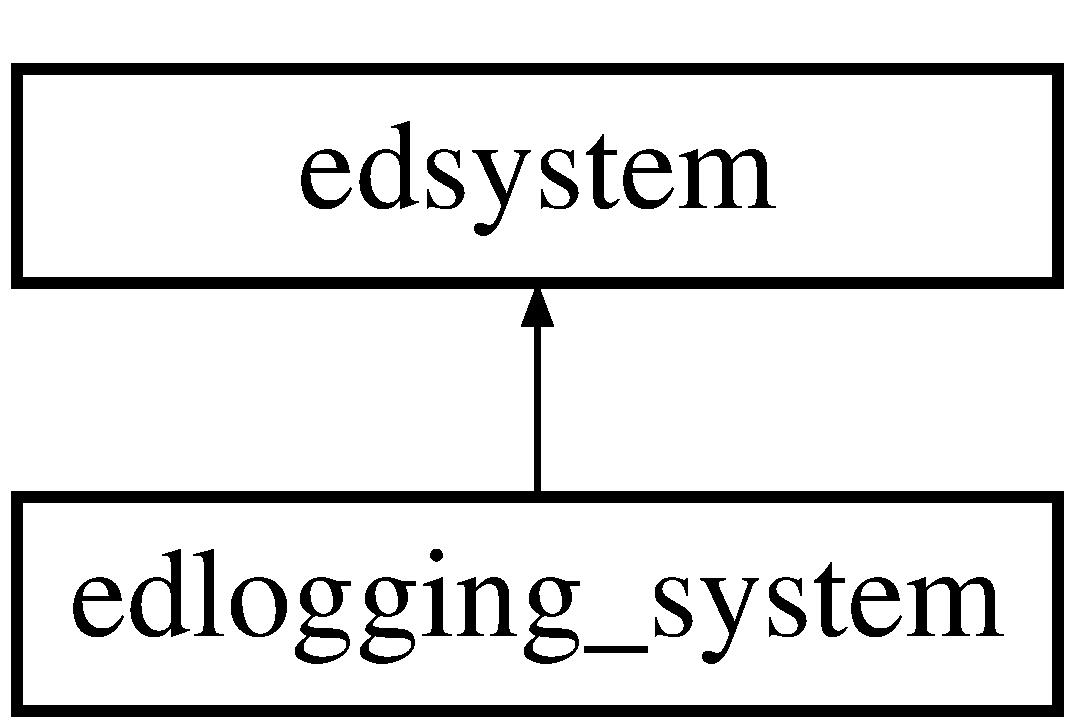
\includegraphics[height=2.000000cm]{classedlogging__system}
\end{center}
\end{figure}
\subsection*{Public Member Functions}
\begin{DoxyCompactItemize}
\item 
\hyperlink{classedlogging__system_ad42113de3431c1655171133d9737a911}{edlogging\-\_\-system} ()
\item 
virtual \hyperlink{classedlogging__system_a0a8901c2649e1d0341fcfb9131e64a72}{$\sim$edlogging\-\_\-system} ()
\item 
virtual void \hyperlink{classedlogging__system_a393094d06bb5d15155be58286f0a5185}{init} ()
\item 
virtual void \hyperlink{classedlogging__system_ad959e6d140397e22953b2b7d1738456a}{release} ()
\item 
virtual bool \hyperlink{classedlogging__system_aa1d63881863c61a89e80aa8187b8d19d}{process} (\hyperlink{structedmessage}{edmessage} $\ast$msg)
\item 
virtual void \hyperlink{classedlogging__system_ac9b9dd8d391244acdea02666a56f8440}{update} ()
\item 
virtual std\-::string \hyperlink{classedlogging__system_ad1262db654a7d7acee6b217a09588170}{typestr} ()
\end{DoxyCompactItemize}
\subsection*{Static Public Member Functions}
\begin{DoxyCompactItemize}
\item 
static std\-::string \hyperlink{classedlogging__system_a5839237a03a9902f0c2311fc3b664f7b}{Type\-String} ()
\end{DoxyCompactItemize}


\subsection{Constructor \& Destructor Documentation}
\hypertarget{classedlogging__system_ad42113de3431c1655171133d9737a911}{\index{edlogging\-\_\-system@{edlogging\-\_\-system}!edlogging\-\_\-system@{edlogging\-\_\-system}}
\index{edlogging\-\_\-system@{edlogging\-\_\-system}!edlogging_system@{edlogging\-\_\-system}}
\subsubsection[{edlogging\-\_\-system}]{\setlength{\rightskip}{0pt plus 5cm}edlogging\-\_\-system\-::edlogging\-\_\-system (
\begin{DoxyParamCaption}
{}
\end{DoxyParamCaption}
)\hspace{0.3cm}{\ttfamily [inline]}}}\label{classedlogging__system_ad42113de3431c1655171133d9737a911}
\hypertarget{classedlogging__system_a0a8901c2649e1d0341fcfb9131e64a72}{\index{edlogging\-\_\-system@{edlogging\-\_\-system}!$\sim$edlogging\-\_\-system@{$\sim$edlogging\-\_\-system}}
\index{$\sim$edlogging\-\_\-system@{$\sim$edlogging\-\_\-system}!edlogging_system@{edlogging\-\_\-system}}
\subsubsection[{$\sim$edlogging\-\_\-system}]{\setlength{\rightskip}{0pt plus 5cm}virtual edlogging\-\_\-system\-::$\sim$edlogging\-\_\-system (
\begin{DoxyParamCaption}
{}
\end{DoxyParamCaption}
)\hspace{0.3cm}{\ttfamily [inline]}, {\ttfamily [virtual]}}}\label{classedlogging__system_a0a8901c2649e1d0341fcfb9131e64a72}


\subsection{Member Function Documentation}
\hypertarget{classedlogging__system_a393094d06bb5d15155be58286f0a5185}{\index{edlogging\-\_\-system@{edlogging\-\_\-system}!init@{init}}
\index{init@{init}!edlogging_system@{edlogging\-\_\-system}}
\subsubsection[{init}]{\setlength{\rightskip}{0pt plus 5cm}void edlogging\-\_\-system\-::init (
\begin{DoxyParamCaption}
{}
\end{DoxyParamCaption}
)\hspace{0.3cm}{\ttfamily [virtual]}}}\label{classedlogging__system_a393094d06bb5d15155be58286f0a5185}


Implements \hyperlink{classedsystem_a4c70e3568064941607fb220aea826a56}{edsystem}.

\hypertarget{classedlogging__system_aa1d63881863c61a89e80aa8187b8d19d}{\index{edlogging\-\_\-system@{edlogging\-\_\-system}!process@{process}}
\index{process@{process}!edlogging_system@{edlogging\-\_\-system}}
\subsubsection[{process}]{\setlength{\rightskip}{0pt plus 5cm}bool edlogging\-\_\-system\-::process (
\begin{DoxyParamCaption}
\item[{{\bf edmessage} $\ast$}]{msg}
\end{DoxyParamCaption}
)\hspace{0.3cm}{\ttfamily [virtual]}}}\label{classedlogging__system_aa1d63881863c61a89e80aa8187b8d19d}


Implements \hyperlink{classedsystem_a9d7a0547c702af1572ed8a1f5434fa0a}{edsystem}.

\hypertarget{classedlogging__system_ad959e6d140397e22953b2b7d1738456a}{\index{edlogging\-\_\-system@{edlogging\-\_\-system}!release@{release}}
\index{release@{release}!edlogging_system@{edlogging\-\_\-system}}
\subsubsection[{release}]{\setlength{\rightskip}{0pt plus 5cm}void edlogging\-\_\-system\-::release (
\begin{DoxyParamCaption}
{}
\end{DoxyParamCaption}
)\hspace{0.3cm}{\ttfamily [virtual]}}}\label{classedlogging__system_ad959e6d140397e22953b2b7d1738456a}


Implements \hyperlink{classedsystem_af40ac185ca4a8efd6777fdb4c65880ea}{edsystem}.

\hypertarget{classedlogging__system_ad1262db654a7d7acee6b217a09588170}{\index{edlogging\-\_\-system@{edlogging\-\_\-system}!typestr@{typestr}}
\index{typestr@{typestr}!edlogging_system@{edlogging\-\_\-system}}
\subsubsection[{typestr}]{\setlength{\rightskip}{0pt plus 5cm}virtual std\-::string edlogging\-\_\-system\-::typestr (
\begin{DoxyParamCaption}
{}
\end{DoxyParamCaption}
)\hspace{0.3cm}{\ttfamily [inline]}, {\ttfamily [virtual]}}}\label{classedlogging__system_ad1262db654a7d7acee6b217a09588170}


Implements \hyperlink{classedsystem_a19dc65111f9a38259fcafba3a32a646d}{edsystem}.

\hypertarget{classedlogging__system_a5839237a03a9902f0c2311fc3b664f7b}{\index{edlogging\-\_\-system@{edlogging\-\_\-system}!Type\-String@{Type\-String}}
\index{Type\-String@{Type\-String}!edlogging_system@{edlogging\-\_\-system}}
\subsubsection[{Type\-String}]{\setlength{\rightskip}{0pt plus 5cm}static std\-::string edlogging\-\_\-system\-::\-Type\-String (
\begin{DoxyParamCaption}
{}
\end{DoxyParamCaption}
)\hspace{0.3cm}{\ttfamily [inline]}, {\ttfamily [static]}}}\label{classedlogging__system_a5839237a03a9902f0c2311fc3b664f7b}
\hypertarget{classedlogging__system_ac9b9dd8d391244acdea02666a56f8440}{\index{edlogging\-\_\-system@{edlogging\-\_\-system}!update@{update}}
\index{update@{update}!edlogging_system@{edlogging\-\_\-system}}
\subsubsection[{update}]{\setlength{\rightskip}{0pt plus 5cm}void edlogging\-\_\-system\-::update (
\begin{DoxyParamCaption}
{}
\end{DoxyParamCaption}
)\hspace{0.3cm}{\ttfamily [virtual]}}}\label{classedlogging__system_ac9b9dd8d391244acdea02666a56f8440}


Implements \hyperlink{classedsystem_afd5308dc71350fe4e239cac5fb1bdbe9}{edsystem}.



The documentation for this class was generated from the following files\-:\begin{DoxyCompactItemize}
\item 
/home/dprandle/\-Documents/code/ctrlmod/include/\hyperlink{edlogging__system_8h}{edlogging\-\_\-system.\-h}\item 
/home/dprandle/\-Documents/code/ctrlmod/src/\hyperlink{edlogging__system_8cpp}{edlogging\-\_\-system.\-cpp}\end{DoxyCompactItemize}

\hypertarget{classedmctrl}{\section{edmctrl Class Reference}
\label{classedmctrl}\index{edmctrl@{edmctrl}}
}


{\ttfamily \#include $<$edmctrl.\-h$>$}

\subsection*{Public Member Functions}
\begin{DoxyCompactItemize}
\item 
\hyperlink{classedmctrl_a4b7377b0608a92535a951caff22dbf51}{edmctrl} ()
\item 
virtual \hyperlink{classedmctrl_a4b76af2c6a4a327dae683582f73f89bf}{$\sim$edmctrl} ()
\item 
{\footnotesize template$<$class T $>$ }\\T $\ast$ \hyperlink{classedmctrl_acf2444928f98bbd396f65022ab60e6d6}{add\-\_\-sys} ()
\item 
bool \hyperlink{classedmctrl_a0dd1befe6818fcbd97419b947ffcd154}{running} ()
\item 
void \hyperlink{classedmctrl_a6b507d894977d67d598b4930521f27fa}{init} ()
\item 
void \hyperlink{classedmctrl_ad82a90b7c2c08479118607febfcadd87}{release} ()
\item 
\hyperlink{classedmessage__dispatch}{edmessage\-\_\-dispatch} $\ast$ \hyperlink{classedmctrl_a96e74e3995d187b3023fdf4ef9b2dc88}{message\-\_\-dispatch} ()
\item 
void \hyperlink{classedmctrl_aeed744e39caf7ab6fdc1004c8cf69a8d}{start} ()
\item 
void \hyperlink{classedmctrl_a36276dab82db9d425268e277dcf5fcb3}{stop} ()
\item 
\hyperlink{classedtimer}{edtimer} $\ast$ \hyperlink{classedmctrl_aa77d5e27f2665fb1c09c29cd057ec09c}{sys\-\_\-timer} ()
\item 
void \hyperlink{classedmctrl_ad9e0ab19fd2b723aedd558b0af130d6a}{update} ()
\item 
{\footnotesize template$<$class T $>$ }\\void \hyperlink{classedmctrl_a3050d02e3f473fb5638aa5c3e77a7d88}{rm\-\_\-sys} ()
\item 
void \hyperlink{classedmctrl_adb9621c87a43535ea084912387e894b8}{rm\-\_\-sys} (const std\-::string \&sysname)
\item 
{\footnotesize template$<$class T $>$ }\\T $\ast$ \hyperlink{classedmctrl_a0be60e649d1981d69099c023bc579bf3}{sys} ()
\item 
\hyperlink{classedsystem}{edsystem} $\ast$ \hyperlink{classedmctrl_a0f434a10847a095073f0897f839e428c}{sys} (const std\-::string \&sysname)
\end{DoxyCompactItemize}
\subsection*{Static Public Member Functions}
\begin{DoxyCompactItemize}
\item 
static \hyperlink{classedmctrl}{edmctrl} \& \hyperlink{classedmctrl_a5977247f3379a9e39709a07303ffef90}{inst} ()
\item 
static void \hyperlink{classedmctrl_a27c76a331f287950479999ab2b112906}{quit} (void)
\end{DoxyCompactItemize}


\subsection{Constructor \& Destructor Documentation}
\hypertarget{classedmctrl_a4b7377b0608a92535a951caff22dbf51}{\index{edmctrl@{edmctrl}!edmctrl@{edmctrl}}
\index{edmctrl@{edmctrl}!edmctrl@{edmctrl}}
\subsubsection[{edmctrl}]{\setlength{\rightskip}{0pt plus 5cm}edmctrl\-::edmctrl (
\begin{DoxyParamCaption}
{}
\end{DoxyParamCaption}
)}}\label{classedmctrl_a4b7377b0608a92535a951caff22dbf51}
\hypertarget{classedmctrl_a4b76af2c6a4a327dae683582f73f89bf}{\index{edmctrl@{edmctrl}!$\sim$edmctrl@{$\sim$edmctrl}}
\index{$\sim$edmctrl@{$\sim$edmctrl}!edmctrl@{edmctrl}}
\subsubsection[{$\sim$edmctrl}]{\setlength{\rightskip}{0pt plus 5cm}edmctrl\-::$\sim$edmctrl (
\begin{DoxyParamCaption}
{}
\end{DoxyParamCaption}
)\hspace{0.3cm}{\ttfamily [virtual]}}}\label{classedmctrl_a4b76af2c6a4a327dae683582f73f89bf}


\subsection{Member Function Documentation}
\hypertarget{classedmctrl_acf2444928f98bbd396f65022ab60e6d6}{\index{edmctrl@{edmctrl}!add\-\_\-sys@{add\-\_\-sys}}
\index{add\-\_\-sys@{add\-\_\-sys}!edmctrl@{edmctrl}}
\subsubsection[{add\-\_\-sys}]{\setlength{\rightskip}{0pt plus 5cm}template$<$class T $>$ T$\ast$ edmctrl\-::add\-\_\-sys (
\begin{DoxyParamCaption}
{}
\end{DoxyParamCaption}
)\hspace{0.3cm}{\ttfamily [inline]}}}\label{classedmctrl_acf2444928f98bbd396f65022ab60e6d6}
\hypertarget{classedmctrl_a6b507d894977d67d598b4930521f27fa}{\index{edmctrl@{edmctrl}!init@{init}}
\index{init@{init}!edmctrl@{edmctrl}}
\subsubsection[{init}]{\setlength{\rightskip}{0pt plus 5cm}void edmctrl\-::init (
\begin{DoxyParamCaption}
{}
\end{DoxyParamCaption}
)}}\label{classedmctrl_a6b507d894977d67d598b4930521f27fa}
\hypertarget{classedmctrl_a5977247f3379a9e39709a07303ffef90}{\index{edmctrl@{edmctrl}!inst@{inst}}
\index{inst@{inst}!edmctrl@{edmctrl}}
\subsubsection[{inst}]{\setlength{\rightskip}{0pt plus 5cm}{\bf edmctrl} \& edmctrl\-::inst (
\begin{DoxyParamCaption}
{}
\end{DoxyParamCaption}
)\hspace{0.3cm}{\ttfamily [static]}}}\label{classedmctrl_a5977247f3379a9e39709a07303ffef90}
\hypertarget{classedmctrl_a96e74e3995d187b3023fdf4ef9b2dc88}{\index{edmctrl@{edmctrl}!message\-\_\-dispatch@{message\-\_\-dispatch}}
\index{message\-\_\-dispatch@{message\-\_\-dispatch}!edmctrl@{edmctrl}}
\subsubsection[{message\-\_\-dispatch}]{\setlength{\rightskip}{0pt plus 5cm}{\bf edmessage\-\_\-dispatch} $\ast$ edmctrl\-::message\-\_\-dispatch (
\begin{DoxyParamCaption}
{}
\end{DoxyParamCaption}
)}}\label{classedmctrl_a96e74e3995d187b3023fdf4ef9b2dc88}
\hypertarget{classedmctrl_a27c76a331f287950479999ab2b112906}{\index{edmctrl@{edmctrl}!quit@{quit}}
\index{quit@{quit}!edmctrl@{edmctrl}}
\subsubsection[{quit}]{\setlength{\rightskip}{0pt plus 5cm}void edmctrl\-::quit (
\begin{DoxyParamCaption}
\item[{void}]{}
\end{DoxyParamCaption}
)\hspace{0.3cm}{\ttfamily [static]}}}\label{classedmctrl_a27c76a331f287950479999ab2b112906}
\hypertarget{classedmctrl_ad82a90b7c2c08479118607febfcadd87}{\index{edmctrl@{edmctrl}!release@{release}}
\index{release@{release}!edmctrl@{edmctrl}}
\subsubsection[{release}]{\setlength{\rightskip}{0pt plus 5cm}void edmctrl\-::release (
\begin{DoxyParamCaption}
{}
\end{DoxyParamCaption}
)}}\label{classedmctrl_ad82a90b7c2c08479118607febfcadd87}
\hypertarget{classedmctrl_a3050d02e3f473fb5638aa5c3e77a7d88}{\index{edmctrl@{edmctrl}!rm\-\_\-sys@{rm\-\_\-sys}}
\index{rm\-\_\-sys@{rm\-\_\-sys}!edmctrl@{edmctrl}}
\subsubsection[{rm\-\_\-sys}]{\setlength{\rightskip}{0pt plus 5cm}template$<$class T $>$ void edmctrl\-::rm\-\_\-sys (
\begin{DoxyParamCaption}
{}
\end{DoxyParamCaption}
)\hspace{0.3cm}{\ttfamily [inline]}}}\label{classedmctrl_a3050d02e3f473fb5638aa5c3e77a7d88}
\hypertarget{classedmctrl_adb9621c87a43535ea084912387e894b8}{\index{edmctrl@{edmctrl}!rm\-\_\-sys@{rm\-\_\-sys}}
\index{rm\-\_\-sys@{rm\-\_\-sys}!edmctrl@{edmctrl}}
\subsubsection[{rm\-\_\-sys}]{\setlength{\rightskip}{0pt plus 5cm}void edmctrl\-::rm\-\_\-sys (
\begin{DoxyParamCaption}
\item[{const std\-::string \&}]{sysname}
\end{DoxyParamCaption}
)}}\label{classedmctrl_adb9621c87a43535ea084912387e894b8}
\hypertarget{classedmctrl_a0dd1befe6818fcbd97419b947ffcd154}{\index{edmctrl@{edmctrl}!running@{running}}
\index{running@{running}!edmctrl@{edmctrl}}
\subsubsection[{running}]{\setlength{\rightskip}{0pt plus 5cm}bool edmctrl\-::running (
\begin{DoxyParamCaption}
{}
\end{DoxyParamCaption}
)}}\label{classedmctrl_a0dd1befe6818fcbd97419b947ffcd154}
\hypertarget{classedmctrl_aeed744e39caf7ab6fdc1004c8cf69a8d}{\index{edmctrl@{edmctrl}!start@{start}}
\index{start@{start}!edmctrl@{edmctrl}}
\subsubsection[{start}]{\setlength{\rightskip}{0pt plus 5cm}void edmctrl\-::start (
\begin{DoxyParamCaption}
{}
\end{DoxyParamCaption}
)}}\label{classedmctrl_aeed744e39caf7ab6fdc1004c8cf69a8d}
\hypertarget{classedmctrl_a36276dab82db9d425268e277dcf5fcb3}{\index{edmctrl@{edmctrl}!stop@{stop}}
\index{stop@{stop}!edmctrl@{edmctrl}}
\subsubsection[{stop}]{\setlength{\rightskip}{0pt plus 5cm}void edmctrl\-::stop (
\begin{DoxyParamCaption}
{}
\end{DoxyParamCaption}
)}}\label{classedmctrl_a36276dab82db9d425268e277dcf5fcb3}
\hypertarget{classedmctrl_a0be60e649d1981d69099c023bc579bf3}{\index{edmctrl@{edmctrl}!sys@{sys}}
\index{sys@{sys}!edmctrl@{edmctrl}}
\subsubsection[{sys}]{\setlength{\rightskip}{0pt plus 5cm}template$<$class T $>$ T$\ast$ edmctrl\-::sys (
\begin{DoxyParamCaption}
{}
\end{DoxyParamCaption}
)\hspace{0.3cm}{\ttfamily [inline]}}}\label{classedmctrl_a0be60e649d1981d69099c023bc579bf3}
\hypertarget{classedmctrl_a0f434a10847a095073f0897f839e428c}{\index{edmctrl@{edmctrl}!sys@{sys}}
\index{sys@{sys}!edmctrl@{edmctrl}}
\subsubsection[{sys}]{\setlength{\rightskip}{0pt plus 5cm}{\bf edsystem} $\ast$ edmctrl\-::sys (
\begin{DoxyParamCaption}
\item[{const std\-::string \&}]{sysname}
\end{DoxyParamCaption}
)}}\label{classedmctrl_a0f434a10847a095073f0897f839e428c}
\hypertarget{classedmctrl_aa77d5e27f2665fb1c09c29cd057ec09c}{\index{edmctrl@{edmctrl}!sys\-\_\-timer@{sys\-\_\-timer}}
\index{sys\-\_\-timer@{sys\-\_\-timer}!edmctrl@{edmctrl}}
\subsubsection[{sys\-\_\-timer}]{\setlength{\rightskip}{0pt plus 5cm}{\bf edtimer} $\ast$ edmctrl\-::sys\-\_\-timer (
\begin{DoxyParamCaption}
{}
\end{DoxyParamCaption}
)}}\label{classedmctrl_aa77d5e27f2665fb1c09c29cd057ec09c}
\hypertarget{classedmctrl_ad9e0ab19fd2b723aedd558b0af130d6a}{\index{edmctrl@{edmctrl}!update@{update}}
\index{update@{update}!edmctrl@{edmctrl}}
\subsubsection[{update}]{\setlength{\rightskip}{0pt plus 5cm}void edmctrl\-::update (
\begin{DoxyParamCaption}
{}
\end{DoxyParamCaption}
)}}\label{classedmctrl_ad9e0ab19fd2b723aedd558b0af130d6a}


The documentation for this class was generated from the following files\-:\begin{DoxyCompactItemize}
\item 
/home/dprandle/\-Documents/code/ctrlmod/include/\hyperlink{edmctrl_8h}{edmctrl.\-h}\item 
/home/dprandle/\-Documents/code/ctrlmod/src/\hyperlink{edmctrl_8cpp}{edmctrl.\-cpp}\end{DoxyCompactItemize}

\hypertarget{structedmessage}{\section{edmessage Struct Reference}
\label{structedmessage}\index{edmessage@{edmessage}}
}


{\ttfamily \#include $<$edmessage.\-h$>$}

Inheritance diagram for edmessage\-:\begin{figure}[H]
\begin{center}
\leavevmode
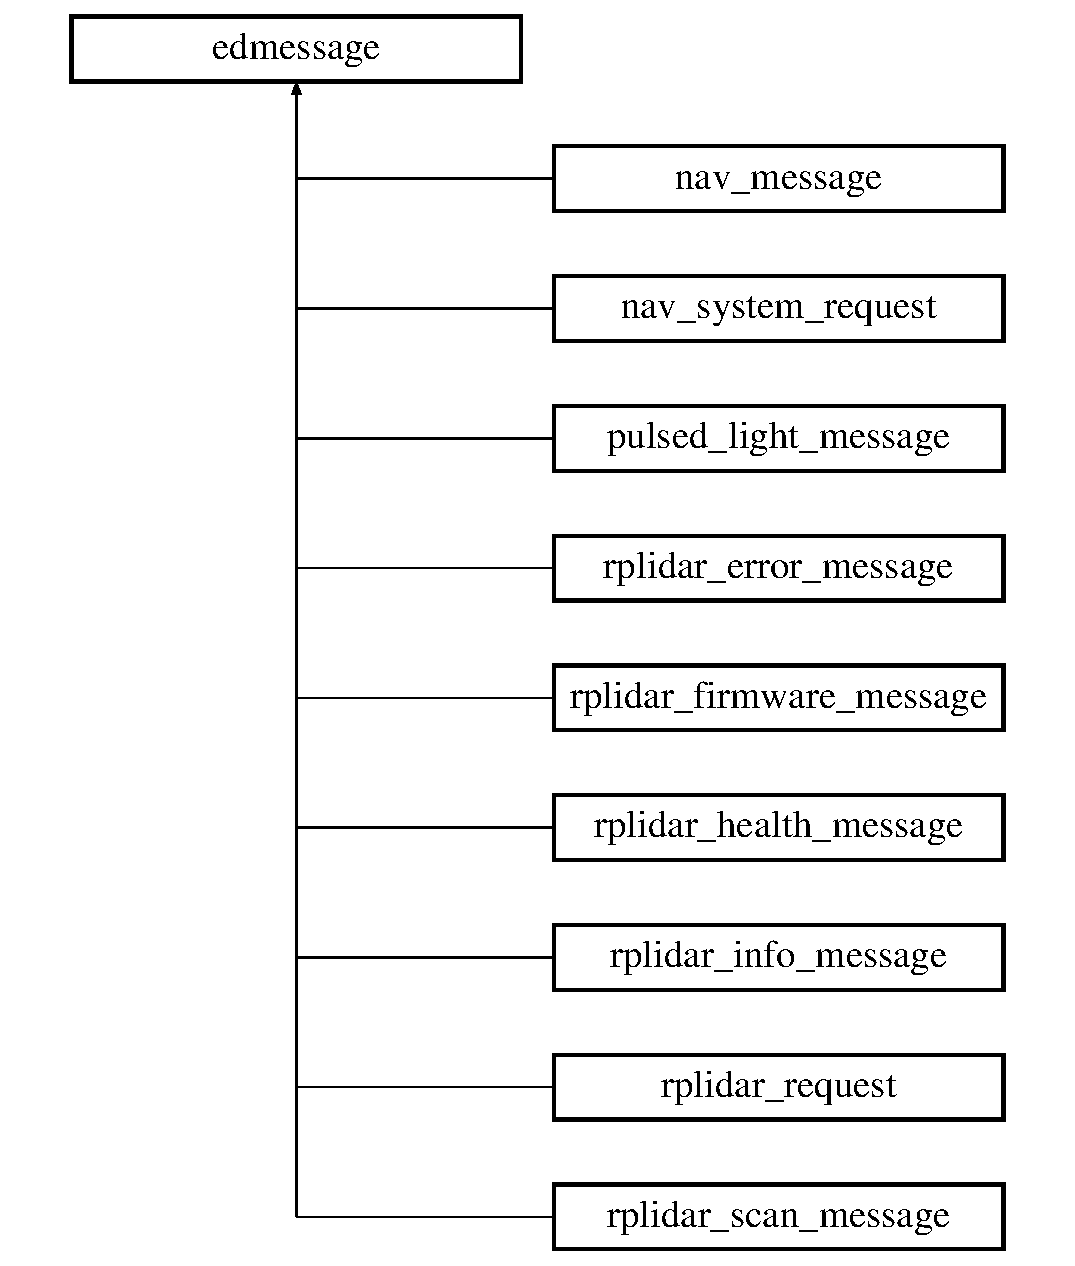
\includegraphics[height=10.000000cm]{structedmessage}
\end{center}
\end{figure}
\subsection*{Public Member Functions}
\begin{DoxyCompactItemize}
\item 
virtual \hyperlink{structedmessage_a4096acc3351b6fca939675b9c53fe288}{$\sim$edmessage} ()
\item 
virtual std\-::string \hyperlink{structedmessage_ac888cf8e570a4aa9bea30a4c4fcdcc30}{type} ()=0
\end{DoxyCompactItemize}
\subsection*{Public Attributes}
\begin{DoxyCompactItemize}
\item 
uint32\-\_\-t \hyperlink{structedmessage_ae9b1f7796892b0433f80a07c4353014f}{ref\-\_\-count}
\end{DoxyCompactItemize}


\subsection{Constructor \& Destructor Documentation}
\hypertarget{structedmessage_a4096acc3351b6fca939675b9c53fe288}{\index{edmessage@{edmessage}!$\sim$edmessage@{$\sim$edmessage}}
\index{$\sim$edmessage@{$\sim$edmessage}!edmessage@{edmessage}}
\subsubsection[{$\sim$edmessage}]{\setlength{\rightskip}{0pt plus 5cm}virtual edmessage\-::$\sim$edmessage (
\begin{DoxyParamCaption}
{}
\end{DoxyParamCaption}
)\hspace{0.3cm}{\ttfamily [inline]}, {\ttfamily [virtual]}}}\label{structedmessage_a4096acc3351b6fca939675b9c53fe288}


\subsection{Member Function Documentation}
\hypertarget{structedmessage_ac888cf8e570a4aa9bea30a4c4fcdcc30}{\index{edmessage@{edmessage}!type@{type}}
\index{type@{type}!edmessage@{edmessage}}
\subsubsection[{type}]{\setlength{\rightskip}{0pt plus 5cm}virtual std\-::string edmessage\-::type (
\begin{DoxyParamCaption}
{}
\end{DoxyParamCaption}
)\hspace{0.3cm}{\ttfamily [pure virtual]}}}\label{structedmessage_ac888cf8e570a4aa9bea30a4c4fcdcc30}


Implemented in \hyperlink{structrplidar__firmware__message_a6985ec56070c19af62cf4b95dbeb78f8}{rplidar\-\_\-firmware\-\_\-message}, \hyperlink{structrplidar__health__message_aa886bee47423f541669914e883b838ee}{rplidar\-\_\-health\-\_\-message}, \hyperlink{structrplidar__info__message_a05bacd569c40d9f88ef4374af34bea49}{rplidar\-\_\-info\-\_\-message}, \hyperlink{structrplidar__error__message_a3041dd23bfc9e0b5612bd7ce75849ea1}{rplidar\-\_\-error\-\_\-message}, \hyperlink{structrplidar__scan__message_aa402778fbabf5375a2a9f229bdb609b6}{rplidar\-\_\-scan\-\_\-message}, \hyperlink{structnav__system__request_aea068f2cdc3e36680b870c0acdfdd111}{nav\-\_\-system\-\_\-request}, \hyperlink{structrplidar__request_af5765bf9fe3d05e9642a255f3b9edfdc}{rplidar\-\_\-request}, \hyperlink{structnav__message_a71d65e9c6328a4f9d2393d010f5fe873}{nav\-\_\-message}, and \hyperlink{structpulsed__light__message_af69b69dbd86e8fb7dc30ee3a304a5e35}{pulsed\-\_\-light\-\_\-message}.



\subsection{Member Data Documentation}
\hypertarget{structedmessage_ae9b1f7796892b0433f80a07c4353014f}{\index{edmessage@{edmessage}!ref\-\_\-count@{ref\-\_\-count}}
\index{ref\-\_\-count@{ref\-\_\-count}!edmessage@{edmessage}}
\subsubsection[{ref\-\_\-count}]{\setlength{\rightskip}{0pt plus 5cm}uint32\-\_\-t edmessage\-::ref\-\_\-count}}\label{structedmessage_ae9b1f7796892b0433f80a07c4353014f}


The documentation for this struct was generated from the following file\-:\begin{DoxyCompactItemize}
\item 
/home/dprandle/\-Documents/code/ctrlmod/include/\hyperlink{edmessage_8h}{edmessage.\-h}\end{DoxyCompactItemize}

\hypertarget{classedmessage__dispatch}{\section{edmessage\-\_\-dispatch Class Reference}
\label{classedmessage__dispatch}\index{edmessage\-\_\-dispatch@{edmessage\-\_\-dispatch}}
}


Class \hyperlink{classedmessage__dispatch}{edmessage\-\_\-dispatch}.  




{\ttfamily \#include $<$edmessage\-\_\-dispatch.\-h$>$}

\subsection*{Public Types}
\begin{DoxyCompactItemize}
\item 
typedef std\-::map$<$ std\-::string, \\*
std\-::set$<$ \hyperlink{classedsystem}{edsystem} $\ast$ $>$ $>$ \hyperlink{classedmessage__dispatch_a6fca76f17817a3296ed712c8a2cc52d1}{listener\-\_\-map}
\item 
typedef std\-::map$<$ \hyperlink{classedsystem}{edsystem} \\*
$\ast$, std\-::deque$<$ \hyperlink{structedmessage}{edmessage} $\ast$ $>$ $>$ \hyperlink{classedmessage__dispatch_a4e1b44916d32280f02e952e0e41774bc}{listener\-\_\-queue}
\end{DoxyCompactItemize}
\subsection*{Public Member Functions}
\begin{DoxyCompactItemize}
\item 
\hyperlink{classedmessage__dispatch_a8eef1480309ce6b3439b649ed5e94fdc}{edmessage\-\_\-dispatch} ()
\item 
virtual \hyperlink{classedmessage__dispatch_ad00ef6c590f2d0aa56ce4ba0c42d8a20}{$\sim$edmessage\-\_\-dispatch} ()
\item 
{\footnotesize template$<$class Message\-Type $>$ }\\void \hyperlink{classedmessage__dispatch_a72e810fc8be900d420c5bc4e4e7ed0fb}{register\-\_\-listener} (\hyperlink{classedsystem}{edsystem} $\ast$sys)
\item 
{\footnotesize template$<$class Message\-Type $>$ }\\void \hyperlink{classedmessage__dispatch_af2e13b40c33728a19f189bc8dd222d3b}{unregister\-\_\-listener} (\hyperlink{classedsystem}{edsystem} $\ast$sys)
\item 
{\footnotesize template$<$class Message\-Type $>$ }\\Message\-Type $\ast$ \hyperlink{classedmessage__dispatch_ab0a4b47e7c90abea073511dc6d72e338}{push} ()
\item 
{\footnotesize template$<$class Message\-Type $>$ }\\Message\-Type $\ast$ \hyperlink{classedmessage__dispatch_acc783ed63b9f2dfe3ddb278d4e7518de}{push\-\_\-front} ()
\item 
\hyperlink{structedmessage}{edmessage} $\ast$ \hyperlink{classedmessage__dispatch_a62ce8628df9d3bc4b62831514ce586b6}{next} (\hyperlink{classedsystem}{edsystem} $\ast$sys)
\item 
void \hyperlink{classedmessage__dispatch_a498a009d4903b42a080ad002021992c3}{pop} (\hyperlink{classedsystem}{edsystem} $\ast$sys)
\item 
void \hyperlink{classedmessage__dispatch_aae298910744e7f59cbf0d1e87b9d7fc2}{process\-\_\-all} (\hyperlink{classedsystem}{edsystem} $\ast$sys)
\end{DoxyCompactItemize}


\subsection{Detailed Description}
Class \hyperlink{classedmessage__dispatch}{edmessage\-\_\-dispatch}. 

A system can register its interest in certain message types, and any time a message of that type is created it will be added to that system's message queue. This queue is F\-I\-F\-O, and messages will not be deleted until they have been removed from every system's message queue.

Systems can process all messages in their queue by calling process\-\_\-all(system$\ast$) where system$\ast$ is a pointer to whatever system messages should be processed for (likely \char`\"{}this\char`\"{} pointer). Messages are processed by calling the respective system's process function over and over until all messages in the system's message que are gone. If process returns false at any point, no more messages will be processed and process\-\_\-all will return.

You can also process one message at a time by calling next to get the oldest message, and pop to remove that message. 

\subsection{Member Typedef Documentation}
\hypertarget{classedmessage__dispatch_a6fca76f17817a3296ed712c8a2cc52d1}{\index{edmessage\-\_\-dispatch@{edmessage\-\_\-dispatch}!listener\-\_\-map@{listener\-\_\-map}}
\index{listener\-\_\-map@{listener\-\_\-map}!edmessage_dispatch@{edmessage\-\_\-dispatch}}
\subsubsection[{listener\-\_\-map}]{\setlength{\rightskip}{0pt plus 5cm}typedef std\-::map$<$ std\-::string, std\-::set$<${\bf edsystem}$\ast$$>$ $>$ {\bf edmessage\-\_\-dispatch\-::listener\-\_\-map}}}\label{classedmessage__dispatch_a6fca76f17817a3296ed712c8a2cc52d1}
This maps message type names to sets of systems. Any system that registers with a message type will be added to the system set corresponding to that message type. \hypertarget{classedmessage__dispatch_a4e1b44916d32280f02e952e0e41774bc}{\index{edmessage\-\_\-dispatch@{edmessage\-\_\-dispatch}!listener\-\_\-queue@{listener\-\_\-queue}}
\index{listener\-\_\-queue@{listener\-\_\-queue}!edmessage_dispatch@{edmessage\-\_\-dispatch}}
\subsubsection[{listener\-\_\-queue}]{\setlength{\rightskip}{0pt plus 5cm}typedef std\-::map$<${\bf edsystem}$\ast$, std\-::deque$<${\bf edmessage}$\ast$$>$ $>$ {\bf edmessage\-\_\-dispatch\-::listener\-\_\-queue}}}\label{classedmessage__dispatch_a4e1b44916d32280f02e952e0e41774bc}
Listener queue holds a map of system pointers to deques of messages. This is F\-I\-F\-O setup -\/ when a message is added to the queue it is appended to the back and when one is taken, it is taken from the front. This does not actually actually delete the message -\/ the message is not deleted until it is no longer in any of the queues. A reference count is kept within the message itself. 

\subsection{Constructor \& Destructor Documentation}
\hypertarget{classedmessage__dispatch_a8eef1480309ce6b3439b649ed5e94fdc}{\index{edmessage\-\_\-dispatch@{edmessage\-\_\-dispatch}!edmessage\-\_\-dispatch@{edmessage\-\_\-dispatch}}
\index{edmessage\-\_\-dispatch@{edmessage\-\_\-dispatch}!edmessage_dispatch@{edmessage\-\_\-dispatch}}
\subsubsection[{edmessage\-\_\-dispatch}]{\setlength{\rightskip}{0pt plus 5cm}edmessage\-\_\-dispatch\-::edmessage\-\_\-dispatch (
\begin{DoxyParamCaption}
{}
\end{DoxyParamCaption}
)}}\label{classedmessage__dispatch_a8eef1480309ce6b3439b649ed5e94fdc}
\hypertarget{classedmessage__dispatch_ad00ef6c590f2d0aa56ce4ba0c42d8a20}{\index{edmessage\-\_\-dispatch@{edmessage\-\_\-dispatch}!$\sim$edmessage\-\_\-dispatch@{$\sim$edmessage\-\_\-dispatch}}
\index{$\sim$edmessage\-\_\-dispatch@{$\sim$edmessage\-\_\-dispatch}!edmessage_dispatch@{edmessage\-\_\-dispatch}}
\subsubsection[{$\sim$edmessage\-\_\-dispatch}]{\setlength{\rightskip}{0pt plus 5cm}edmessage\-\_\-dispatch\-::$\sim$edmessage\-\_\-dispatch (
\begin{DoxyParamCaption}
{}
\end{DoxyParamCaption}
)\hspace{0.3cm}{\ttfamily [virtual]}}}\label{classedmessage__dispatch_ad00ef6c590f2d0aa56ce4ba0c42d8a20}


\subsection{Member Function Documentation}
\hypertarget{classedmessage__dispatch_a62ce8628df9d3bc4b62831514ce586b6}{\index{edmessage\-\_\-dispatch@{edmessage\-\_\-dispatch}!next@{next}}
\index{next@{next}!edmessage_dispatch@{edmessage\-\_\-dispatch}}
\subsubsection[{next}]{\setlength{\rightskip}{0pt plus 5cm}{\bf edmessage} $\ast$ edmessage\-\_\-dispatch\-::next (
\begin{DoxyParamCaption}
\item[{{\bf edsystem} $\ast$}]{sys}
\end{DoxyParamCaption}
)}}\label{classedmessage__dispatch_a62ce8628df9d3bc4b62831514ce586b6}
\hypertarget{classedmessage__dispatch_a498a009d4903b42a080ad002021992c3}{\index{edmessage\-\_\-dispatch@{edmessage\-\_\-dispatch}!pop@{pop}}
\index{pop@{pop}!edmessage_dispatch@{edmessage\-\_\-dispatch}}
\subsubsection[{pop}]{\setlength{\rightskip}{0pt plus 5cm}void edmessage\-\_\-dispatch\-::pop (
\begin{DoxyParamCaption}
\item[{{\bf edsystem} $\ast$}]{sys}
\end{DoxyParamCaption}
)}}\label{classedmessage__dispatch_a498a009d4903b42a080ad002021992c3}
\hypertarget{classedmessage__dispatch_aae298910744e7f59cbf0d1e87b9d7fc2}{\index{edmessage\-\_\-dispatch@{edmessage\-\_\-dispatch}!process\-\_\-all@{process\-\_\-all}}
\index{process\-\_\-all@{process\-\_\-all}!edmessage_dispatch@{edmessage\-\_\-dispatch}}
\subsubsection[{process\-\_\-all}]{\setlength{\rightskip}{0pt plus 5cm}void edmessage\-\_\-dispatch\-::process\-\_\-all (
\begin{DoxyParamCaption}
\item[{{\bf edsystem} $\ast$}]{sys}
\end{DoxyParamCaption}
)}}\label{classedmessage__dispatch_aae298910744e7f59cbf0d1e87b9d7fc2}
\hypertarget{classedmessage__dispatch_ab0a4b47e7c90abea073511dc6d72e338}{\index{edmessage\-\_\-dispatch@{edmessage\-\_\-dispatch}!push@{push}}
\index{push@{push}!edmessage_dispatch@{edmessage\-\_\-dispatch}}
\subsubsection[{push}]{\setlength{\rightskip}{0pt plus 5cm}template$<$class Message\-Type $>$ Message\-Type$\ast$ edmessage\-\_\-dispatch\-::push (
\begin{DoxyParamCaption}
{}
\end{DoxyParamCaption}
)\hspace{0.3cm}{\ttfamily [inline]}}}\label{classedmessage__dispatch_ab0a4b47e7c90abea073511dc6d72e338}
\hypertarget{classedmessage__dispatch_acc783ed63b9f2dfe3ddb278d4e7518de}{\index{edmessage\-\_\-dispatch@{edmessage\-\_\-dispatch}!push\-\_\-front@{push\-\_\-front}}
\index{push\-\_\-front@{push\-\_\-front}!edmessage_dispatch@{edmessage\-\_\-dispatch}}
\subsubsection[{push\-\_\-front}]{\setlength{\rightskip}{0pt plus 5cm}template$<$class Message\-Type $>$ Message\-Type$\ast$ edmessage\-\_\-dispatch\-::push\-\_\-front (
\begin{DoxyParamCaption}
{}
\end{DoxyParamCaption}
)\hspace{0.3cm}{\ttfamily [inline]}}}\label{classedmessage__dispatch_acc783ed63b9f2dfe3ddb278d4e7518de}
\hypertarget{classedmessage__dispatch_a72e810fc8be900d420c5bc4e4e7ed0fb}{\index{edmessage\-\_\-dispatch@{edmessage\-\_\-dispatch}!register\-\_\-listener@{register\-\_\-listener}}
\index{register\-\_\-listener@{register\-\_\-listener}!edmessage_dispatch@{edmessage\-\_\-dispatch}}
\subsubsection[{register\-\_\-listener}]{\setlength{\rightskip}{0pt plus 5cm}template$<$class Message\-Type $>$ void edmessage\-\_\-dispatch\-::register\-\_\-listener (
\begin{DoxyParamCaption}
\item[{{\bf edsystem} $\ast$}]{sys}
\end{DoxyParamCaption}
)\hspace{0.3cm}{\ttfamily [inline]}}}\label{classedmessage__dispatch_a72e810fc8be900d420c5bc4e4e7ed0fb}
\hypertarget{classedmessage__dispatch_af2e13b40c33728a19f189bc8dd222d3b}{\index{edmessage\-\_\-dispatch@{edmessage\-\_\-dispatch}!unregister\-\_\-listener@{unregister\-\_\-listener}}
\index{unregister\-\_\-listener@{unregister\-\_\-listener}!edmessage_dispatch@{edmessage\-\_\-dispatch}}
\subsubsection[{unregister\-\_\-listener}]{\setlength{\rightskip}{0pt plus 5cm}template$<$class Message\-Type $>$ void edmessage\-\_\-dispatch\-::unregister\-\_\-listener (
\begin{DoxyParamCaption}
\item[{{\bf edsystem} $\ast$}]{sys}
\end{DoxyParamCaption}
)\hspace{0.3cm}{\ttfamily [inline]}}}\label{classedmessage__dispatch_af2e13b40c33728a19f189bc8dd222d3b}


The documentation for this class was generated from the following files\-:\begin{DoxyCompactItemize}
\item 
/home/dprandle/\-Documents/code/ctrlmod/include/\hyperlink{edmessage__dispatch_8h}{edmessage\-\_\-dispatch.\-h}\item 
/home/dprandle/\-Documents/code/ctrlmod/src/\hyperlink{edmessage__dispatch_8cpp}{edmessage\-\_\-dispatch.\-cpp}\end{DoxyCompactItemize}

\hypertarget{classednav__system}{\section{ednav\-\_\-system Class Reference}
\label{classednav__system}\index{ednav\-\_\-system@{ednav\-\_\-system}}
}


{\ttfamily \#include $<$ednavsystem.\-h$>$}

Inheritance diagram for ednav\-\_\-system\-:\begin{figure}[H]
\begin{center}
\leavevmode
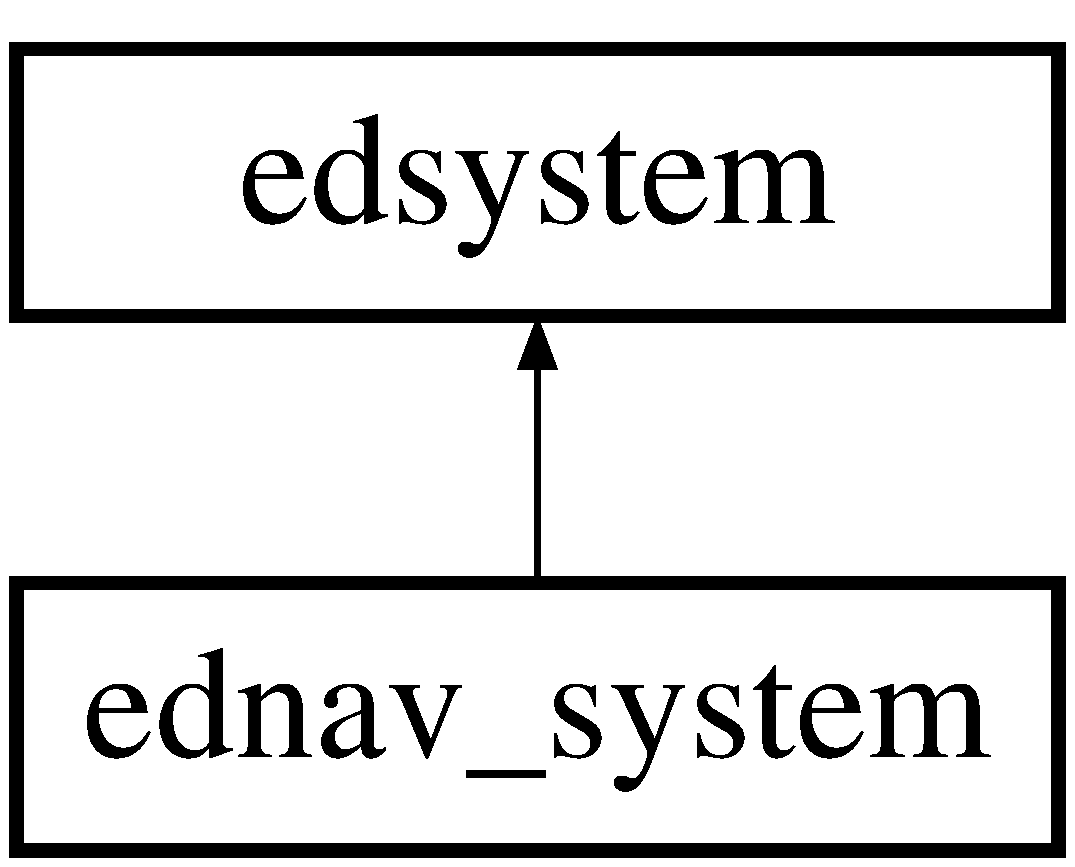
\includegraphics[height=2.000000cm]{classednav__system}
\end{center}
\end{figure}
\subsection*{Public Member Functions}
\begin{DoxyCompactItemize}
\item 
\hyperlink{classednav__system_ab9f404145bc9a1c21f221da04e73726a}{ednav\-\_\-system} ()
\item 
virtual \hyperlink{classednav__system_a81d991d9380e3cd80f0c65e8ccf35f40}{$\sim$ednav\-\_\-system} ()
\item 
virtual void \hyperlink{classednav__system_a98bc9b1cecf79a6ca7145e34a0273ca2}{init} ()
\item 
virtual void \hyperlink{classednav__system_aa41383e31657188e5386b45d4dd7e4cd}{release} ()
\item 
virtual bool \hyperlink{classednav__system_ae90088e1c3a01fdeb0fc051af71e6d6a}{process} (\hyperlink{structedmessage}{edmessage} $\ast$msg)
\item 
virtual void \hyperlink{classednav__system_a3a32c9f0ee4c089ac2e0eff9dae9a879}{update} ()
\item 
double \hyperlink{classednav__system_ae99f310450a1ec9a2e106db05d90f96a}{interval} ()
\item 
void \hyperlink{classednav__system_a6648f9731b39a60fbdef7c254aa341ac}{set\-\_\-interval} (double ms)
\item 
virtual std\-::string \hyperlink{classednav__system_a3d604cf5dcff8c1c7d8c492e213c1e3c}{typestr} ()
\end{DoxyCompactItemize}
\subsection*{Static Public Member Functions}
\begin{DoxyCompactItemize}
\item 
static std\-::string \hyperlink{classednav__system_a28e8f447138e00c50320044c85ae9bce}{Type\-String} ()
\end{DoxyCompactItemize}
\subsection*{Friends}
\begin{DoxyCompactItemize}
\item 
struct \hyperlink{classednav__system_a2fddae920e343f1b3d243c06003fe73c}{instruction\-\_\-callback}
\end{DoxyCompactItemize}


\subsection{Constructor \& Destructor Documentation}
\hypertarget{classednav__system_ab9f404145bc9a1c21f221da04e73726a}{\index{ednav\-\_\-system@{ednav\-\_\-system}!ednav\-\_\-system@{ednav\-\_\-system}}
\index{ednav\-\_\-system@{ednav\-\_\-system}!ednav_system@{ednav\-\_\-system}}
\subsubsection[{ednav\-\_\-system}]{\setlength{\rightskip}{0pt plus 5cm}ednav\-\_\-system\-::ednav\-\_\-system (
\begin{DoxyParamCaption}
{}
\end{DoxyParamCaption}
)}}\label{classednav__system_ab9f404145bc9a1c21f221da04e73726a}
\hypertarget{classednav__system_a81d991d9380e3cd80f0c65e8ccf35f40}{\index{ednav\-\_\-system@{ednav\-\_\-system}!$\sim$ednav\-\_\-system@{$\sim$ednav\-\_\-system}}
\index{$\sim$ednav\-\_\-system@{$\sim$ednav\-\_\-system}!ednav_system@{ednav\-\_\-system}}
\subsubsection[{$\sim$ednav\-\_\-system}]{\setlength{\rightskip}{0pt plus 5cm}ednav\-\_\-system\-::$\sim$ednav\-\_\-system (
\begin{DoxyParamCaption}
{}
\end{DoxyParamCaption}
)\hspace{0.3cm}{\ttfamily [virtual]}}}\label{classednav__system_a81d991d9380e3cd80f0c65e8ccf35f40}


\subsection{Member Function Documentation}
\hypertarget{classednav__system_a98bc9b1cecf79a6ca7145e34a0273ca2}{\index{ednav\-\_\-system@{ednav\-\_\-system}!init@{init}}
\index{init@{init}!ednav_system@{ednav\-\_\-system}}
\subsubsection[{init}]{\setlength{\rightskip}{0pt plus 5cm}void ednav\-\_\-system\-::init (
\begin{DoxyParamCaption}
{}
\end{DoxyParamCaption}
)\hspace{0.3cm}{\ttfamily [virtual]}}}\label{classednav__system_a98bc9b1cecf79a6ca7145e34a0273ca2}


Implements \hyperlink{classedsystem_a4c70e3568064941607fb220aea826a56}{edsystem}.

\hypertarget{classednav__system_ae99f310450a1ec9a2e106db05d90f96a}{\index{ednav\-\_\-system@{ednav\-\_\-system}!interval@{interval}}
\index{interval@{interval}!ednav_system@{ednav\-\_\-system}}
\subsubsection[{interval}]{\setlength{\rightskip}{0pt plus 5cm}double ednav\-\_\-system\-::interval (
\begin{DoxyParamCaption}
{}
\end{DoxyParamCaption}
)}}\label{classednav__system_ae99f310450a1ec9a2e106db05d90f96a}
\hypertarget{classednav__system_ae90088e1c3a01fdeb0fc051af71e6d6a}{\index{ednav\-\_\-system@{ednav\-\_\-system}!process@{process}}
\index{process@{process}!ednav_system@{ednav\-\_\-system}}
\subsubsection[{process}]{\setlength{\rightskip}{0pt plus 5cm}bool ednav\-\_\-system\-::process (
\begin{DoxyParamCaption}
\item[{{\bf edmessage} $\ast$}]{msg}
\end{DoxyParamCaption}
)\hspace{0.3cm}{\ttfamily [virtual]}}}\label{classednav__system_ae90088e1c3a01fdeb0fc051af71e6d6a}


Implements \hyperlink{classedsystem_a9d7a0547c702af1572ed8a1f5434fa0a}{edsystem}.

\hypertarget{classednav__system_aa41383e31657188e5386b45d4dd7e4cd}{\index{ednav\-\_\-system@{ednav\-\_\-system}!release@{release}}
\index{release@{release}!ednav_system@{ednav\-\_\-system}}
\subsubsection[{release}]{\setlength{\rightskip}{0pt plus 5cm}void ednav\-\_\-system\-::release (
\begin{DoxyParamCaption}
{}
\end{DoxyParamCaption}
)\hspace{0.3cm}{\ttfamily [virtual]}}}\label{classednav__system_aa41383e31657188e5386b45d4dd7e4cd}


Implements \hyperlink{classedsystem_af40ac185ca4a8efd6777fdb4c65880ea}{edsystem}.

\hypertarget{classednav__system_a6648f9731b39a60fbdef7c254aa341ac}{\index{ednav\-\_\-system@{ednav\-\_\-system}!set\-\_\-interval@{set\-\_\-interval}}
\index{set\-\_\-interval@{set\-\_\-interval}!ednav_system@{ednav\-\_\-system}}
\subsubsection[{set\-\_\-interval}]{\setlength{\rightskip}{0pt plus 5cm}void ednav\-\_\-system\-::set\-\_\-interval (
\begin{DoxyParamCaption}
\item[{double}]{ms}
\end{DoxyParamCaption}
)}}\label{classednav__system_a6648f9731b39a60fbdef7c254aa341ac}
\hypertarget{classednav__system_a3d604cf5dcff8c1c7d8c492e213c1e3c}{\index{ednav\-\_\-system@{ednav\-\_\-system}!typestr@{typestr}}
\index{typestr@{typestr}!ednav_system@{ednav\-\_\-system}}
\subsubsection[{typestr}]{\setlength{\rightskip}{0pt plus 5cm}virtual std\-::string ednav\-\_\-system\-::typestr (
\begin{DoxyParamCaption}
{}
\end{DoxyParamCaption}
)\hspace{0.3cm}{\ttfamily [inline]}, {\ttfamily [virtual]}}}\label{classednav__system_a3d604cf5dcff8c1c7d8c492e213c1e3c}


Implements \hyperlink{classedsystem_a19dc65111f9a38259fcafba3a32a646d}{edsystem}.

\hypertarget{classednav__system_a28e8f447138e00c50320044c85ae9bce}{\index{ednav\-\_\-system@{ednav\-\_\-system}!Type\-String@{Type\-String}}
\index{Type\-String@{Type\-String}!ednav_system@{ednav\-\_\-system}}
\subsubsection[{Type\-String}]{\setlength{\rightskip}{0pt plus 5cm}static std\-::string ednav\-\_\-system\-::\-Type\-String (
\begin{DoxyParamCaption}
{}
\end{DoxyParamCaption}
)\hspace{0.3cm}{\ttfamily [inline]}, {\ttfamily [static]}}}\label{classednav__system_a28e8f447138e00c50320044c85ae9bce}
\hypertarget{classednav__system_a3a32c9f0ee4c089ac2e0eff9dae9a879}{\index{ednav\-\_\-system@{ednav\-\_\-system}!update@{update}}
\index{update@{update}!ednav_system@{ednav\-\_\-system}}
\subsubsection[{update}]{\setlength{\rightskip}{0pt plus 5cm}void ednav\-\_\-system\-::update (
\begin{DoxyParamCaption}
{}
\end{DoxyParamCaption}
)\hspace{0.3cm}{\ttfamily [virtual]}}}\label{classednav__system_a3a32c9f0ee4c089ac2e0eff9dae9a879}


Implements \hyperlink{classedsystem_afd5308dc71350fe4e239cac5fb1bdbe9}{edsystem}.



\subsection{Friends And Related Function Documentation}
\hypertarget{classednav__system_a2fddae920e343f1b3d243c06003fe73c}{\index{ednav\-\_\-system@{ednav\-\_\-system}!instruction\-\_\-callback@{instruction\-\_\-callback}}
\index{instruction\-\_\-callback@{instruction\-\_\-callback}!ednav_system@{ednav\-\_\-system}}
\subsubsection[{instruction\-\_\-callback}]{\setlength{\rightskip}{0pt plus 5cm}friend struct {\bf instruction\-\_\-callback}\hspace{0.3cm}{\ttfamily [friend]}}}\label{classednav__system_a2fddae920e343f1b3d243c06003fe73c}


The documentation for this class was generated from the following files\-:\begin{DoxyCompactItemize}
\item 
/home/dprandle/\-Documents/code/ctrlmod/include/\hyperlink{ednavsystem_8h}{ednavsystem.\-h}\item 
/home/dprandle/\-Documents/code/ctrlmod/src/\hyperlink{ednavsystem_8cpp}{ednavsystem.\-cpp}\end{DoxyCompactItemize}

\hypertarget{classedpid__controller}{\section{edpid\-\_\-controller$<$ T $>$ Class Template Reference}
\label{classedpid__controller}\index{edpid\-\_\-controller$<$ T $>$@{edpid\-\_\-controller$<$ T $>$}}
}


{\ttfamily \#include $<$edpid\-\_\-controller.\-h$>$}

\subsection*{Classes}
\begin{DoxyCompactItemize}
\item 
struct \hyperlink{structedpid__controller_1_1output__range}{output\-\_\-range}
\end{DoxyCompactItemize}
\subsection*{Public Member Functions}
\begin{DoxyCompactItemize}
\item 
\hyperlink{classedpid__controller_a6008f5babbd8bc9141e5abba929ef790}{edpid\-\_\-controller} ()
\item 
\hyperlink{classedpid__controller_a683ec5f02e55d19b7ec2675fe0190f71}{$\sim$edpid\-\_\-controller} ()
\item 
void \hyperlink{classedpid__controller_a3f0c19167813e4030edec7f42a0d0661}{enable\-\_\-complex\-\_\-derivitive} (bool enable)
\item 
void \hyperlink{classedpid__controller_aa04a42b0f58b8eb752a463cb56afab6f}{enable\-\_\-anti\-\_\-reset\-\_\-windup} (bool enable)
\item 
bool \hyperlink{classedpid__controller_a88f516cfe3bb8d3e95f2d5dfd923d646}{anti\-\_\-reset\-\_\-windup} ()
\item 
bool \hyperlink{classedpid__controller_a9946eac8a4f3181706d54ba8bd96026f}{complex\-\_\-derivitive} ()
\item 
const \hyperlink{nsmath_8h_a14bb8a4a0fefc0be4fae32fc59a07362}{vec3} \& \hyperlink{classedpid__controller_a4a8906107d15d7a917444ee98c703f7d}{gain} ()
\item 
double \hyperlink{classedpid__controller_a2e7e231001cd92137021664c43d1cc0b}{offset} ()
\item 
const \hyperlink{structedpid__controller_1_1output__range}{output\-\_\-range} \& \hyperlink{classedpid__controller_a64befb22b629646521abb29d25c8f14e}{range} ()
\item 
double \hyperlink{classedpid__controller_adb51025b2e94dbd63aa1841e3712100a}{ramp\-\_\-limit} ()
\item 
void \hyperlink{classedpid__controller_a4ec73738276f6cc8fe6df6a82b602f57}{set\-\_\-gain} (const \hyperlink{nsmath_8h_a14bb8a4a0fefc0be4fae32fc59a07362}{vec3} \&pid\-\_\-)
\item 
void \hyperlink{classedpid__controller_a3dbbe642abf4db2cec4c6489896e05bd}{set\-\_\-gain} (double P, double I, double D)
\item 
void \hyperlink{classedpid__controller_ae730045cd6f055530783cf959e97f391}{set\-\_\-gain\-\_\-\-P} (double P)
\item 
void \hyperlink{classedpid__controller_a633260c32c9c7ae2b3c253f56bce57e7}{set\-\_\-gain\-\_\-\-I} (double I)
\item 
void \hyperlink{classedpid__controller_ab591a923cf7398e5514b58cc4e348047}{set\-\_\-gain\-\_\-\-D} (double D)
\item 
void \hyperlink{classedpid__controller_ad568ede08f4e7f7e7ae6806e11fee3f3}{set\-\_\-offset} (double offset\-\_\-)
\item 
void \hyperlink{classedpid__controller_ad5c00d11bbf6a566a85f6db7ec53d13a}{set\-\_\-ramp\-\_\-limit} (double percent)
\item 
void \hyperlink{classedpid__controller_acd29b7081cbaf41da267e47cde944dcf}{set\-\_\-range} (const T \&\hyperlink{nsvec4_8h_a02ad6e0792741c9c15dd05d27bcb80e6}{min}, const T \&\hyperlink{nsvec4_8h_a4c6db3c946e82dd750cfb4494ddc4b47}{max})
\item 
void \hyperlink{classedpid__controller_a4a3b487d6e7df82254565fd8c336b58c}{set\-\_\-target} (const T \&target\-\_\-)
\item 
T \hyperlink{classedpid__controller_a9b5038f14a975a7e3ddc87d7e3bd9c77}{loop} (const T \&input, double dt)
\item 
const T \& \hyperlink{classedpid__controller_a5b23219adc085dd6cbc054acae30e5f2}{target} ()
\end{DoxyCompactItemize}


\subsection{Constructor \& Destructor Documentation}
\hypertarget{classedpid__controller_a6008f5babbd8bc9141e5abba929ef790}{\index{edpid\-\_\-controller@{edpid\-\_\-controller}!edpid\-\_\-controller@{edpid\-\_\-controller}}
\index{edpid\-\_\-controller@{edpid\-\_\-controller}!edpid_controller@{edpid\-\_\-controller}}
\subsubsection[{edpid\-\_\-controller}]{\setlength{\rightskip}{0pt plus 5cm}template$<$class T $>$ {\bf edpid\-\_\-controller}$<$ T $>$\-::{\bf edpid\-\_\-controller} (
\begin{DoxyParamCaption}
{}
\end{DoxyParamCaption}
)}}\label{classedpid__controller_a6008f5babbd8bc9141e5abba929ef790}
\hypertarget{classedpid__controller_a683ec5f02e55d19b7ec2675fe0190f71}{\index{edpid\-\_\-controller@{edpid\-\_\-controller}!$\sim$edpid\-\_\-controller@{$\sim$edpid\-\_\-controller}}
\index{$\sim$edpid\-\_\-controller@{$\sim$edpid\-\_\-controller}!edpid_controller@{edpid\-\_\-controller}}
\subsubsection[{$\sim$edpid\-\_\-controller}]{\setlength{\rightskip}{0pt plus 5cm}template$<$class T $>$ {\bf edpid\-\_\-controller}$<$ T $>$\-::$\sim${\bf edpid\-\_\-controller} (
\begin{DoxyParamCaption}
{}
\end{DoxyParamCaption}
)}}\label{classedpid__controller_a683ec5f02e55d19b7ec2675fe0190f71}


\subsection{Member Function Documentation}
\hypertarget{classedpid__controller_a88f516cfe3bb8d3e95f2d5dfd923d646}{\index{edpid\-\_\-controller@{edpid\-\_\-controller}!anti\-\_\-reset\-\_\-windup@{anti\-\_\-reset\-\_\-windup}}
\index{anti\-\_\-reset\-\_\-windup@{anti\-\_\-reset\-\_\-windup}!edpid_controller@{edpid\-\_\-controller}}
\subsubsection[{anti\-\_\-reset\-\_\-windup}]{\setlength{\rightskip}{0pt plus 5cm}template$<$class T $>$ bool {\bf edpid\-\_\-controller}$<$ T $>$\-::anti\-\_\-reset\-\_\-windup (
\begin{DoxyParamCaption}
{}
\end{DoxyParamCaption}
)}}\label{classedpid__controller_a88f516cfe3bb8d3e95f2d5dfd923d646}
\hypertarget{classedpid__controller_a9946eac8a4f3181706d54ba8bd96026f}{\index{edpid\-\_\-controller@{edpid\-\_\-controller}!complex\-\_\-derivitive@{complex\-\_\-derivitive}}
\index{complex\-\_\-derivitive@{complex\-\_\-derivitive}!edpid_controller@{edpid\-\_\-controller}}
\subsubsection[{complex\-\_\-derivitive}]{\setlength{\rightskip}{0pt plus 5cm}template$<$class T $>$ bool {\bf edpid\-\_\-controller}$<$ T $>$\-::complex\-\_\-derivitive (
\begin{DoxyParamCaption}
{}
\end{DoxyParamCaption}
)}}\label{classedpid__controller_a9946eac8a4f3181706d54ba8bd96026f}
\hypertarget{classedpid__controller_aa04a42b0f58b8eb752a463cb56afab6f}{\index{edpid\-\_\-controller@{edpid\-\_\-controller}!enable\-\_\-anti\-\_\-reset\-\_\-windup@{enable\-\_\-anti\-\_\-reset\-\_\-windup}}
\index{enable\-\_\-anti\-\_\-reset\-\_\-windup@{enable\-\_\-anti\-\_\-reset\-\_\-windup}!edpid_controller@{edpid\-\_\-controller}}
\subsubsection[{enable\-\_\-anti\-\_\-reset\-\_\-windup}]{\setlength{\rightskip}{0pt plus 5cm}template$<$class T $>$ void {\bf edpid\-\_\-controller}$<$ T $>$\-::enable\-\_\-anti\-\_\-reset\-\_\-windup (
\begin{DoxyParamCaption}
\item[{bool}]{enable}
\end{DoxyParamCaption}
)}}\label{classedpid__controller_aa04a42b0f58b8eb752a463cb56afab6f}
\hypertarget{classedpid__controller_a3f0c19167813e4030edec7f42a0d0661}{\index{edpid\-\_\-controller@{edpid\-\_\-controller}!enable\-\_\-complex\-\_\-derivitive@{enable\-\_\-complex\-\_\-derivitive}}
\index{enable\-\_\-complex\-\_\-derivitive@{enable\-\_\-complex\-\_\-derivitive}!edpid_controller@{edpid\-\_\-controller}}
\subsubsection[{enable\-\_\-complex\-\_\-derivitive}]{\setlength{\rightskip}{0pt plus 5cm}template$<$class T $>$ void {\bf edpid\-\_\-controller}$<$ T $>$\-::enable\-\_\-complex\-\_\-derivitive (
\begin{DoxyParamCaption}
\item[{bool}]{enable}
\end{DoxyParamCaption}
)}}\label{classedpid__controller_a3f0c19167813e4030edec7f42a0d0661}
\hypertarget{classedpid__controller_a4a8906107d15d7a917444ee98c703f7d}{\index{edpid\-\_\-controller@{edpid\-\_\-controller}!gain@{gain}}
\index{gain@{gain}!edpid_controller@{edpid\-\_\-controller}}
\subsubsection[{gain}]{\setlength{\rightskip}{0pt plus 5cm}template$<$class T $>$ const {\bf vec3} \& {\bf edpid\-\_\-controller}$<$ T $>$\-::gain (
\begin{DoxyParamCaption}
{}
\end{DoxyParamCaption}
)}}\label{classedpid__controller_a4a8906107d15d7a917444ee98c703f7d}
\hypertarget{classedpid__controller_a9b5038f14a975a7e3ddc87d7e3bd9c77}{\index{edpid\-\_\-controller@{edpid\-\_\-controller}!loop@{loop}}
\index{loop@{loop}!edpid_controller@{edpid\-\_\-controller}}
\subsubsection[{loop}]{\setlength{\rightskip}{0pt plus 5cm}template$<$class T$>$ T {\bf edpid\-\_\-controller}$<$ T $>$\-::loop (
\begin{DoxyParamCaption}
\item[{const T \&}]{input, }
\item[{double}]{dt}
\end{DoxyParamCaption}
)}}\label{classedpid__controller_a9b5038f14a975a7e3ddc87d7e3bd9c77}
\hypertarget{classedpid__controller_a2e7e231001cd92137021664c43d1cc0b}{\index{edpid\-\_\-controller@{edpid\-\_\-controller}!offset@{offset}}
\index{offset@{offset}!edpid_controller@{edpid\-\_\-controller}}
\subsubsection[{offset}]{\setlength{\rightskip}{0pt plus 5cm}template$<$class T $>$ double {\bf edpid\-\_\-controller}$<$ T $>$\-::offset (
\begin{DoxyParamCaption}
{}
\end{DoxyParamCaption}
)}}\label{classedpid__controller_a2e7e231001cd92137021664c43d1cc0b}
\hypertarget{classedpid__controller_adb51025b2e94dbd63aa1841e3712100a}{\index{edpid\-\_\-controller@{edpid\-\_\-controller}!ramp\-\_\-limit@{ramp\-\_\-limit}}
\index{ramp\-\_\-limit@{ramp\-\_\-limit}!edpid_controller@{edpid\-\_\-controller}}
\subsubsection[{ramp\-\_\-limit}]{\setlength{\rightskip}{0pt plus 5cm}template$<$class T $>$ double {\bf edpid\-\_\-controller}$<$ T $>$\-::ramp\-\_\-limit (
\begin{DoxyParamCaption}
{}
\end{DoxyParamCaption}
)}}\label{classedpid__controller_adb51025b2e94dbd63aa1841e3712100a}
\hypertarget{classedpid__controller_a64befb22b629646521abb29d25c8f14e}{\index{edpid\-\_\-controller@{edpid\-\_\-controller}!range@{range}}
\index{range@{range}!edpid_controller@{edpid\-\_\-controller}}
\subsubsection[{range}]{\setlength{\rightskip}{0pt plus 5cm}template$<$class T $>$ const {\bf edpid\-\_\-controller}$<$ T $>$\-::{\bf output\-\_\-range} \& {\bf edpid\-\_\-controller}$<$ T $>$\-::range (
\begin{DoxyParamCaption}
{}
\end{DoxyParamCaption}
)}}\label{classedpid__controller_a64befb22b629646521abb29d25c8f14e}
\hypertarget{classedpid__controller_a4ec73738276f6cc8fe6df6a82b602f57}{\index{edpid\-\_\-controller@{edpid\-\_\-controller}!set\-\_\-gain@{set\-\_\-gain}}
\index{set\-\_\-gain@{set\-\_\-gain}!edpid_controller@{edpid\-\_\-controller}}
\subsubsection[{set\-\_\-gain}]{\setlength{\rightskip}{0pt plus 5cm}template$<$class T $>$ void {\bf edpid\-\_\-controller}$<$ T $>$\-::set\-\_\-gain (
\begin{DoxyParamCaption}
\item[{const {\bf vec3} \&}]{pid\-\_\-}
\end{DoxyParamCaption}
)}}\label{classedpid__controller_a4ec73738276f6cc8fe6df6a82b602f57}
\hypertarget{classedpid__controller_a3dbbe642abf4db2cec4c6489896e05bd}{\index{edpid\-\_\-controller@{edpid\-\_\-controller}!set\-\_\-gain@{set\-\_\-gain}}
\index{set\-\_\-gain@{set\-\_\-gain}!edpid_controller@{edpid\-\_\-controller}}
\subsubsection[{set\-\_\-gain}]{\setlength{\rightskip}{0pt plus 5cm}template$<$class T $>$ void {\bf edpid\-\_\-controller}$<$ T $>$\-::set\-\_\-gain (
\begin{DoxyParamCaption}
\item[{double}]{P, }
\item[{double}]{I, }
\item[{double}]{D}
\end{DoxyParamCaption}
)}}\label{classedpid__controller_a3dbbe642abf4db2cec4c6489896e05bd}
\hypertarget{classedpid__controller_ab591a923cf7398e5514b58cc4e348047}{\index{edpid\-\_\-controller@{edpid\-\_\-controller}!set\-\_\-gain\-\_\-\-D@{set\-\_\-gain\-\_\-\-D}}
\index{set\-\_\-gain\-\_\-\-D@{set\-\_\-gain\-\_\-\-D}!edpid_controller@{edpid\-\_\-controller}}
\subsubsection[{set\-\_\-gain\-\_\-\-D}]{\setlength{\rightskip}{0pt plus 5cm}template$<$class T $>$ void {\bf edpid\-\_\-controller}$<$ T $>$\-::set\-\_\-gain\-\_\-\-D (
\begin{DoxyParamCaption}
\item[{double}]{D}
\end{DoxyParamCaption}
)}}\label{classedpid__controller_ab591a923cf7398e5514b58cc4e348047}
\hypertarget{classedpid__controller_a633260c32c9c7ae2b3c253f56bce57e7}{\index{edpid\-\_\-controller@{edpid\-\_\-controller}!set\-\_\-gain\-\_\-\-I@{set\-\_\-gain\-\_\-\-I}}
\index{set\-\_\-gain\-\_\-\-I@{set\-\_\-gain\-\_\-\-I}!edpid_controller@{edpid\-\_\-controller}}
\subsubsection[{set\-\_\-gain\-\_\-\-I}]{\setlength{\rightskip}{0pt plus 5cm}template$<$class T $>$ void {\bf edpid\-\_\-controller}$<$ T $>$\-::set\-\_\-gain\-\_\-\-I (
\begin{DoxyParamCaption}
\item[{double}]{I}
\end{DoxyParamCaption}
)}}\label{classedpid__controller_a633260c32c9c7ae2b3c253f56bce57e7}
\hypertarget{classedpid__controller_ae730045cd6f055530783cf959e97f391}{\index{edpid\-\_\-controller@{edpid\-\_\-controller}!set\-\_\-gain\-\_\-\-P@{set\-\_\-gain\-\_\-\-P}}
\index{set\-\_\-gain\-\_\-\-P@{set\-\_\-gain\-\_\-\-P}!edpid_controller@{edpid\-\_\-controller}}
\subsubsection[{set\-\_\-gain\-\_\-\-P}]{\setlength{\rightskip}{0pt plus 5cm}template$<$class T $>$ void {\bf edpid\-\_\-controller}$<$ T $>$\-::set\-\_\-gain\-\_\-\-P (
\begin{DoxyParamCaption}
\item[{double}]{P}
\end{DoxyParamCaption}
)}}\label{classedpid__controller_ae730045cd6f055530783cf959e97f391}
\hypertarget{classedpid__controller_ad568ede08f4e7f7e7ae6806e11fee3f3}{\index{edpid\-\_\-controller@{edpid\-\_\-controller}!set\-\_\-offset@{set\-\_\-offset}}
\index{set\-\_\-offset@{set\-\_\-offset}!edpid_controller@{edpid\-\_\-controller}}
\subsubsection[{set\-\_\-offset}]{\setlength{\rightskip}{0pt plus 5cm}template$<$class T $>$ void {\bf edpid\-\_\-controller}$<$ T $>$\-::set\-\_\-offset (
\begin{DoxyParamCaption}
\item[{double}]{offset\-\_\-}
\end{DoxyParamCaption}
)}}\label{classedpid__controller_ad568ede08f4e7f7e7ae6806e11fee3f3}
\hypertarget{classedpid__controller_ad5c00d11bbf6a566a85f6db7ec53d13a}{\index{edpid\-\_\-controller@{edpid\-\_\-controller}!set\-\_\-ramp\-\_\-limit@{set\-\_\-ramp\-\_\-limit}}
\index{set\-\_\-ramp\-\_\-limit@{set\-\_\-ramp\-\_\-limit}!edpid_controller@{edpid\-\_\-controller}}
\subsubsection[{set\-\_\-ramp\-\_\-limit}]{\setlength{\rightskip}{0pt plus 5cm}template$<$class T $>$ void {\bf edpid\-\_\-controller}$<$ T $>$\-::set\-\_\-ramp\-\_\-limit (
\begin{DoxyParamCaption}
\item[{double}]{percent}
\end{DoxyParamCaption}
)}}\label{classedpid__controller_ad5c00d11bbf6a566a85f6db7ec53d13a}
\hypertarget{classedpid__controller_acd29b7081cbaf41da267e47cde944dcf}{\index{edpid\-\_\-controller@{edpid\-\_\-controller}!set\-\_\-range@{set\-\_\-range}}
\index{set\-\_\-range@{set\-\_\-range}!edpid_controller@{edpid\-\_\-controller}}
\subsubsection[{set\-\_\-range}]{\setlength{\rightskip}{0pt plus 5cm}template$<$class T$>$ void {\bf edpid\-\_\-controller}$<$ T $>$\-::set\-\_\-range (
\begin{DoxyParamCaption}
\item[{const T \&}]{min, }
\item[{const T \&}]{max}
\end{DoxyParamCaption}
)}}\label{classedpid__controller_acd29b7081cbaf41da267e47cde944dcf}
\hypertarget{classedpid__controller_a4a3b487d6e7df82254565fd8c336b58c}{\index{edpid\-\_\-controller@{edpid\-\_\-controller}!set\-\_\-target@{set\-\_\-target}}
\index{set\-\_\-target@{set\-\_\-target}!edpid_controller@{edpid\-\_\-controller}}
\subsubsection[{set\-\_\-target}]{\setlength{\rightskip}{0pt plus 5cm}template$<$class T$>$ void {\bf edpid\-\_\-controller}$<$ T $>$\-::set\-\_\-target (
\begin{DoxyParamCaption}
\item[{const T \&}]{target\-\_\-}
\end{DoxyParamCaption}
)}}\label{classedpid__controller_a4a3b487d6e7df82254565fd8c336b58c}
\hypertarget{classedpid__controller_a5b23219adc085dd6cbc054acae30e5f2}{\index{edpid\-\_\-controller@{edpid\-\_\-controller}!target@{target}}
\index{target@{target}!edpid_controller@{edpid\-\_\-controller}}
\subsubsection[{target}]{\setlength{\rightskip}{0pt plus 5cm}template$<$class T $>$ const T \& {\bf edpid\-\_\-controller}$<$ T $>$\-::target (
\begin{DoxyParamCaption}
{}
\end{DoxyParamCaption}
)}}\label{classedpid__controller_a5b23219adc085dd6cbc054acae30e5f2}


The documentation for this class was generated from the following file\-:\begin{DoxyCompactItemize}
\item 
/home/dprandle/\-Documents/code/ctrlmod/include/\hyperlink{edpid__controller_8h}{edpid\-\_\-controller.\-h}\end{DoxyCompactItemize}

\hypertarget{structedpl__callback}{\section{edpl\-\_\-callback Struct Reference}
\label{structedpl__callback}\index{edpl\-\_\-callback@{edpl\-\_\-callback}}
}


{\ttfamily \#include $<$edplsystem.\-h$>$}

Inheritance diagram for edpl\-\_\-callback\-:\begin{figure}[H]
\begin{center}
\leavevmode
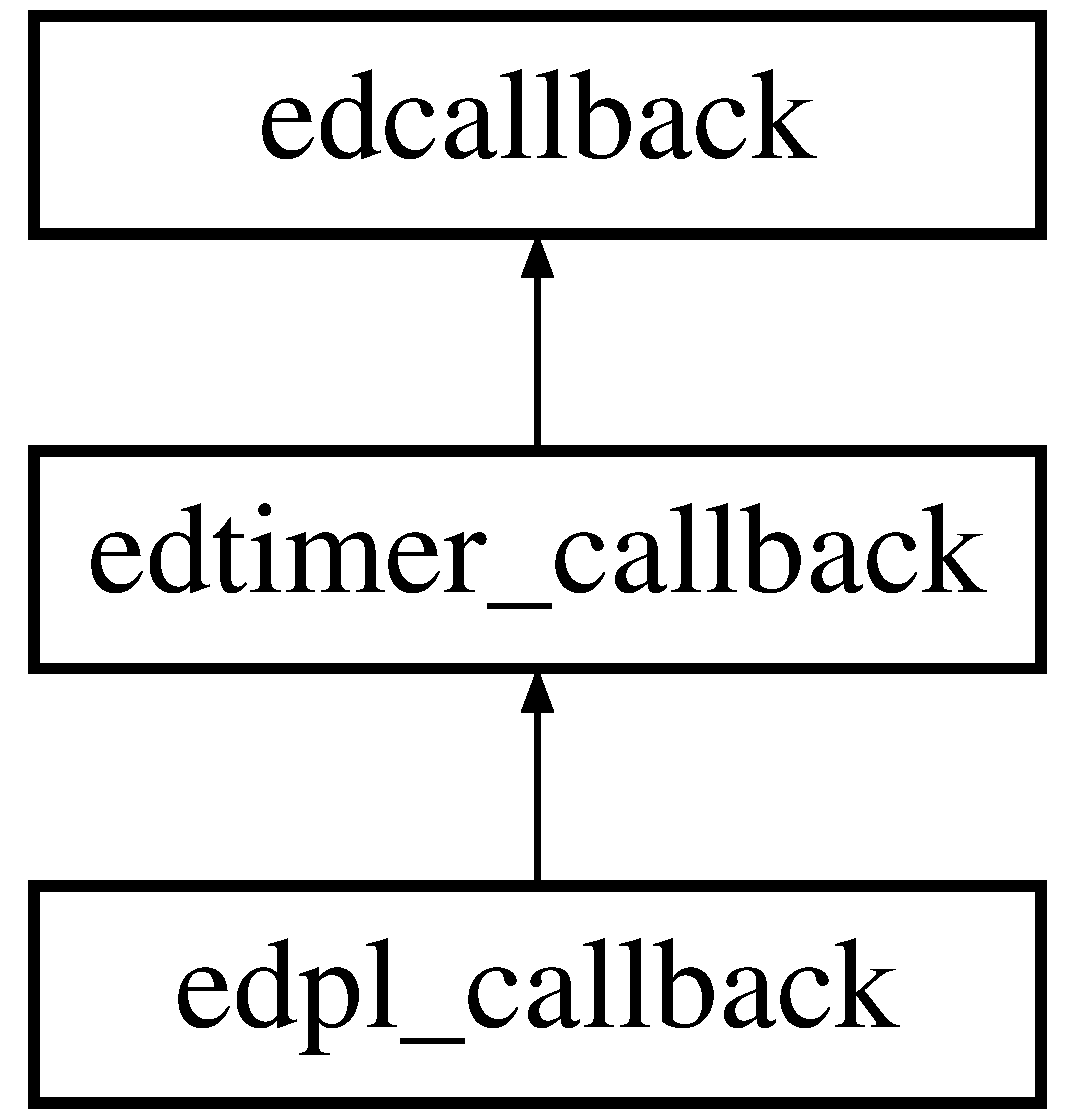
\includegraphics[height=3.000000cm]{structedpl__callback}
\end{center}
\end{figure}
\subsection*{Public Member Functions}
\begin{DoxyCompactItemize}
\item 
\hyperlink{structedpl__callback_ad921d4f126d38a6e2e7769a507c75caf}{edpl\-\_\-callback} (\hyperlink{structedpl__system_1_1pl__gpio}{edpl\-\_\-system\-::pl\-\_\-gpio} $\ast$\hyperlink{nsvec4_8h_a83b4b86a11bb43587ae7fa2d3d1f3856}{ceil}, \hyperlink{structedpl__system_1_1pl__gpio}{edpl\-\_\-system\-::pl\-\_\-gpio} $\ast$\hyperlink{nsvec4_8h_a0409361f2277fca322689ffb014595c0}{floor})
\item 
void \hyperlink{structedpl__callback_a23c8aacf97d5a080af1f7d84439122c8}{exec} ()
\end{DoxyCompactItemize}
\subsection*{Public Attributes}
\begin{DoxyCompactItemize}
\item 
\hyperlink{structedpl__system_1_1pl__gpio}{edpl\-\_\-system\-::pl\-\_\-gpio} $\ast$ \hyperlink{structedpl__callback_acab7f06faf5fb508993d61e47f07da75}{pl\-\_\-ceil}
\item 
\hyperlink{structedpl__system_1_1pl__gpio}{edpl\-\_\-system\-::pl\-\_\-gpio} $\ast$ \hyperlink{structedpl__callback_a6f63343abef0d00077beadfb3a05aab6}{pl\-\_\-floor}
\end{DoxyCompactItemize}


\subsection{Constructor \& Destructor Documentation}
\hypertarget{structedpl__callback_ad921d4f126d38a6e2e7769a507c75caf}{\index{edpl\-\_\-callback@{edpl\-\_\-callback}!edpl\-\_\-callback@{edpl\-\_\-callback}}
\index{edpl\-\_\-callback@{edpl\-\_\-callback}!edpl_callback@{edpl\-\_\-callback}}
\subsubsection[{edpl\-\_\-callback}]{\setlength{\rightskip}{0pt plus 5cm}edpl\-\_\-callback\-::edpl\-\_\-callback (
\begin{DoxyParamCaption}
\item[{{\bf edpl\-\_\-system\-::pl\-\_\-gpio} $\ast$}]{ceil, }
\item[{{\bf edpl\-\_\-system\-::pl\-\_\-gpio} $\ast$}]{floor}
\end{DoxyParamCaption}
)\hspace{0.3cm}{\ttfamily [inline]}}}\label{structedpl__callback_ad921d4f126d38a6e2e7769a507c75caf}


\subsection{Member Function Documentation}
\hypertarget{structedpl__callback_a23c8aacf97d5a080af1f7d84439122c8}{\index{edpl\-\_\-callback@{edpl\-\_\-callback}!exec@{exec}}
\index{exec@{exec}!edpl_callback@{edpl\-\_\-callback}}
\subsubsection[{exec}]{\setlength{\rightskip}{0pt plus 5cm}void edpl\-\_\-callback\-::exec (
\begin{DoxyParamCaption}
{}
\end{DoxyParamCaption}
)\hspace{0.3cm}{\ttfamily [virtual]}}}\label{structedpl__callback_a23c8aacf97d5a080af1f7d84439122c8}


Implements \hyperlink{structedcallback_ab8003af2178e58a94f53370b1f48a313}{edcallback}.



\subsection{Member Data Documentation}
\hypertarget{structedpl__callback_acab7f06faf5fb508993d61e47f07da75}{\index{edpl\-\_\-callback@{edpl\-\_\-callback}!pl\-\_\-ceil@{pl\-\_\-ceil}}
\index{pl\-\_\-ceil@{pl\-\_\-ceil}!edpl_callback@{edpl\-\_\-callback}}
\subsubsection[{pl\-\_\-ceil}]{\setlength{\rightskip}{0pt plus 5cm}{\bf edpl\-\_\-system\-::pl\-\_\-gpio}$\ast$ edpl\-\_\-callback\-::pl\-\_\-ceil}}\label{structedpl__callback_acab7f06faf5fb508993d61e47f07da75}
\hypertarget{structedpl__callback_a6f63343abef0d00077beadfb3a05aab6}{\index{edpl\-\_\-callback@{edpl\-\_\-callback}!pl\-\_\-floor@{pl\-\_\-floor}}
\index{pl\-\_\-floor@{pl\-\_\-floor}!edpl_callback@{edpl\-\_\-callback}}
\subsubsection[{pl\-\_\-floor}]{\setlength{\rightskip}{0pt plus 5cm}{\bf edpl\-\_\-system\-::pl\-\_\-gpio}$\ast$ edpl\-\_\-callback\-::pl\-\_\-floor}}\label{structedpl__callback_a6f63343abef0d00077beadfb3a05aab6}


The documentation for this struct was generated from the following files\-:\begin{DoxyCompactItemize}
\item 
/home/dprandle/\-Documents/code/ctrlmod/include/\hyperlink{edplsystem_8h}{edplsystem.\-h}\item 
/home/dprandle/\-Documents/code/ctrlmod/src/\hyperlink{edplsystem_8cpp}{edplsystem.\-cpp}\end{DoxyCompactItemize}

\hypertarget{classedpl__system}{\section{edpl\-\_\-system Class Reference}
\label{classedpl__system}\index{edpl\-\_\-system@{edpl\-\_\-system}}
}


{\ttfamily \#include $<$edplsystem.\-h$>$}

Inheritance diagram for edpl\-\_\-system\-:\begin{figure}[H]
\begin{center}
\leavevmode
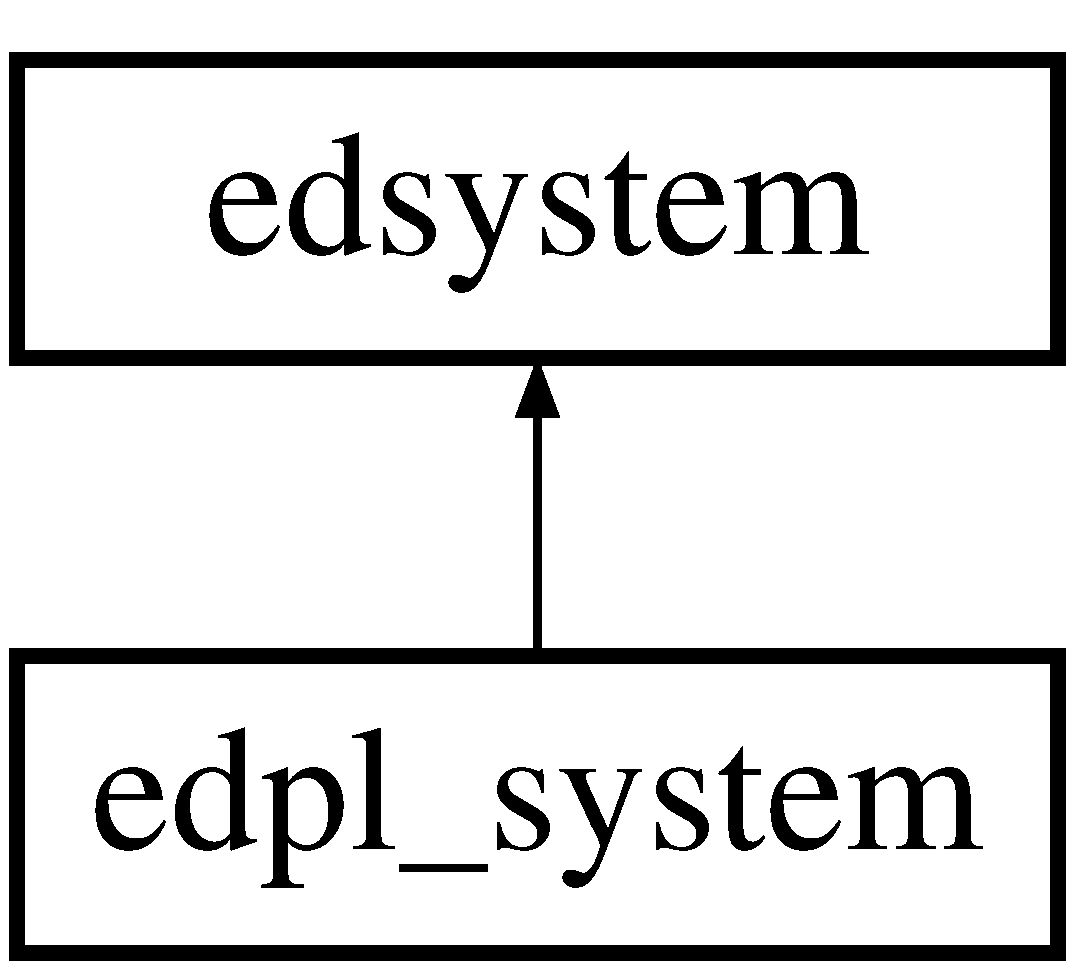
\includegraphics[height=2.000000cm]{classedpl__system}
\end{center}
\end{figure}
\subsection*{Classes}
\begin{DoxyCompactItemize}
\item 
struct \hyperlink{structedpl__system_1_1pl__gpio}{pl\-\_\-gpio}
\end{DoxyCompactItemize}
\subsection*{Public Types}
\begin{DoxyCompactItemize}
\item 
typedef std\-::map$<$ uint32\-\_\-t, \\*
\hyperlink{structedpl__system_1_1pl__gpio}{pl\-\_\-gpio} $\ast$ $>$ \hyperlink{classedpl__system_ac6e43a24e97887c11e2e4d7c54294bc4}{plmap}
\end{DoxyCompactItemize}
\subsection*{Public Member Functions}
\begin{DoxyCompactItemize}
\item 
\hyperlink{classedpl__system_a346231e6092910c7dfd6dd962ee25bc5}{edpl\-\_\-system} ()
\item 
virtual \hyperlink{classedpl__system_a94d6ed134e1abd43c4af6ae3d632f462}{$\sim$edpl\-\_\-system} ()
\item 
\hyperlink{structedpl__system_1_1pl__gpio}{pl\-\_\-gpio} $\ast$ \hyperlink{classedpl__system_ae42b9824a6d9626accbd234375f79c09}{add\-\_\-pl} (uint32\-\_\-t mraa\-\_\-pin, double c\-\_\-offset=0.\-0, const \hyperlink{nsmath_8h_a14bb8a4a0fefc0be4fae32fc59a07362}{vec3} \&pos\-\_\-offset=\hyperlink{nsmath_8h_a14bb8a4a0fefc0be4fae32fc59a07362}{vec3}(), const \hyperlink{nsmath_8h_aa07476c74d8e3787a771c94c92354496}{quat} \&orient\-\_\-offset=\hyperlink{nsmath_8h_aa07476c74d8e3787a771c94c92354496}{quat}())
\item 
\hyperlink{structedpl__system_1_1pl__gpio}{pl\-\_\-gpio} $\ast$ \hyperlink{classedpl__system_a4a4369822031f0f4523abc12125d92d1}{get\-\_\-pl} (uint32\-\_\-t mraa\-\_\-pin)
\item 
void \hyperlink{classedpl__system_ab1e65466442581ce851bec4d4bd40459}{rm\-\_\-pl} (uint32\-\_\-t mraa\-\_\-pin)
\item 
bool \hyperlink{classedpl__system_a9a32ffdff7b99e9ad1f6562f508cd12f}{pl\-\_\-pin\-\_\-taken} (uint32\-\_\-t mraa\-\_\-pin)
\item 
void \hyperlink{classedpl__system_a792001c061fe40e388d7c5aaf428f389}{pl\-\_\-set\-\_\-pos} (uint32\-\_\-t mraa\-\_\-pin, const \hyperlink{nsmath_8h_a14bb8a4a0fefc0be4fae32fc59a07362}{vec3} \&pos\-\_\-)
\item 
void \hyperlink{classedpl__system_a8e7eef161b591dd20b5e23fd246ac3f4}{pl\-\_\-set\-\_\-orientation} (uint32\-\_\-t mraa\-\_\-pin, const \hyperlink{nsmath_8h_aa07476c74d8e3787a771c94c92354496}{quat} \&orient\-\_\-)
\item 
void \hyperlink{classedpl__system_a54044ef9b7b84731ada0b6ec425225ea}{pl\-\_\-set\-\_\-cal\-\_\-offset} (uint32\-\_\-t mraa\-\_\-pin, double offset)
\item 
virtual void \hyperlink{classedpl__system_a4d9fae9e10da9cae1f1e7a00e751c933}{init} ()
\item 
virtual void \hyperlink{classedpl__system_adb2b906b466251dc513fb9d669a19e99}{release} ()
\item 
virtual bool \hyperlink{classedpl__system_a4aae16b8695eec7c54ccfaecee9c535c}{process} (\hyperlink{structedmessage}{edmessage} $\ast$msg)
\item 
virtual void \hyperlink{classedpl__system_ae84af8dea7c53fe3219e7cde15ddd43a}{update} ()
\item 
virtual std\-::string \hyperlink{classedpl__system_ab758bc4300926af08e47e0c8b655d8fc}{typestr} ()
\end{DoxyCompactItemize}
\subsection*{Static Public Member Functions}
\begin{DoxyCompactItemize}
\item 
static std\-::string \hyperlink{classedpl__system_a3b3de76e3cf9c7a34cfe17a7d65fbad4}{Type\-String} ()
\end{DoxyCompactItemize}


\subsection{Member Typedef Documentation}
\hypertarget{classedpl__system_ac6e43a24e97887c11e2e4d7c54294bc4}{\index{edpl\-\_\-system@{edpl\-\_\-system}!plmap@{plmap}}
\index{plmap@{plmap}!edpl_system@{edpl\-\_\-system}}
\subsubsection[{plmap}]{\setlength{\rightskip}{0pt plus 5cm}typedef std\-::map$<$uint32\-\_\-t, {\bf pl\-\_\-gpio}$\ast$$>$ {\bf edpl\-\_\-system\-::plmap}}}\label{classedpl__system_ac6e43a24e97887c11e2e4d7c54294bc4}


\subsection{Constructor \& Destructor Documentation}
\hypertarget{classedpl__system_a346231e6092910c7dfd6dd962ee25bc5}{\index{edpl\-\_\-system@{edpl\-\_\-system}!edpl\-\_\-system@{edpl\-\_\-system}}
\index{edpl\-\_\-system@{edpl\-\_\-system}!edpl_system@{edpl\-\_\-system}}
\subsubsection[{edpl\-\_\-system}]{\setlength{\rightskip}{0pt plus 5cm}edpl\-\_\-system\-::edpl\-\_\-system (
\begin{DoxyParamCaption}
{}
\end{DoxyParamCaption}
)}}\label{classedpl__system_a346231e6092910c7dfd6dd962ee25bc5}
\hypertarget{classedpl__system_a94d6ed134e1abd43c4af6ae3d632f462}{\index{edpl\-\_\-system@{edpl\-\_\-system}!$\sim$edpl\-\_\-system@{$\sim$edpl\-\_\-system}}
\index{$\sim$edpl\-\_\-system@{$\sim$edpl\-\_\-system}!edpl_system@{edpl\-\_\-system}}
\subsubsection[{$\sim$edpl\-\_\-system}]{\setlength{\rightskip}{0pt plus 5cm}edpl\-\_\-system\-::$\sim$edpl\-\_\-system (
\begin{DoxyParamCaption}
{}
\end{DoxyParamCaption}
)\hspace{0.3cm}{\ttfamily [virtual]}}}\label{classedpl__system_a94d6ed134e1abd43c4af6ae3d632f462}


\subsection{Member Function Documentation}
\hypertarget{classedpl__system_ae42b9824a6d9626accbd234375f79c09}{\index{edpl\-\_\-system@{edpl\-\_\-system}!add\-\_\-pl@{add\-\_\-pl}}
\index{add\-\_\-pl@{add\-\_\-pl}!edpl_system@{edpl\-\_\-system}}
\subsubsection[{add\-\_\-pl}]{\setlength{\rightskip}{0pt plus 5cm}{\bf edpl\-\_\-system\-::pl\-\_\-gpio} $\ast$ edpl\-\_\-system\-::add\-\_\-pl (
\begin{DoxyParamCaption}
\item[{uint32\-\_\-t}]{mraa\-\_\-pin, }
\item[{double}]{c\-\_\-offset = {\ttfamily 0.0}, }
\item[{const {\bf vec3} \&}]{pos\-\_\-offset = {\ttfamily {\bf vec3}()}, }
\item[{const {\bf quat} \&}]{orient\-\_\-offset = {\ttfamily {\bf quat}()}}
\end{DoxyParamCaption}
)}}\label{classedpl__system_ae42b9824a6d9626accbd234375f79c09}
\hypertarget{classedpl__system_a4a4369822031f0f4523abc12125d92d1}{\index{edpl\-\_\-system@{edpl\-\_\-system}!get\-\_\-pl@{get\-\_\-pl}}
\index{get\-\_\-pl@{get\-\_\-pl}!edpl_system@{edpl\-\_\-system}}
\subsubsection[{get\-\_\-pl}]{\setlength{\rightskip}{0pt plus 5cm}{\bf edpl\-\_\-system\-::pl\-\_\-gpio} $\ast$ edpl\-\_\-system\-::get\-\_\-pl (
\begin{DoxyParamCaption}
\item[{uint32\-\_\-t}]{mraa\-\_\-pin}
\end{DoxyParamCaption}
)}}\label{classedpl__system_a4a4369822031f0f4523abc12125d92d1}
\hypertarget{classedpl__system_a4d9fae9e10da9cae1f1e7a00e751c933}{\index{edpl\-\_\-system@{edpl\-\_\-system}!init@{init}}
\index{init@{init}!edpl_system@{edpl\-\_\-system}}
\subsubsection[{init}]{\setlength{\rightskip}{0pt plus 5cm}void edpl\-\_\-system\-::init (
\begin{DoxyParamCaption}
{}
\end{DoxyParamCaption}
)\hspace{0.3cm}{\ttfamily [virtual]}}}\label{classedpl__system_a4d9fae9e10da9cae1f1e7a00e751c933}


Implements \hyperlink{classedsystem_a4c70e3568064941607fb220aea826a56}{edsystem}.

\hypertarget{classedpl__system_a9a32ffdff7b99e9ad1f6562f508cd12f}{\index{edpl\-\_\-system@{edpl\-\_\-system}!pl\-\_\-pin\-\_\-taken@{pl\-\_\-pin\-\_\-taken}}
\index{pl\-\_\-pin\-\_\-taken@{pl\-\_\-pin\-\_\-taken}!edpl_system@{edpl\-\_\-system}}
\subsubsection[{pl\-\_\-pin\-\_\-taken}]{\setlength{\rightskip}{0pt plus 5cm}bool edpl\-\_\-system\-::pl\-\_\-pin\-\_\-taken (
\begin{DoxyParamCaption}
\item[{uint32\-\_\-t}]{mraa\-\_\-pin}
\end{DoxyParamCaption}
)}}\label{classedpl__system_a9a32ffdff7b99e9ad1f6562f508cd12f}
\hypertarget{classedpl__system_a54044ef9b7b84731ada0b6ec425225ea}{\index{edpl\-\_\-system@{edpl\-\_\-system}!pl\-\_\-set\-\_\-cal\-\_\-offset@{pl\-\_\-set\-\_\-cal\-\_\-offset}}
\index{pl\-\_\-set\-\_\-cal\-\_\-offset@{pl\-\_\-set\-\_\-cal\-\_\-offset}!edpl_system@{edpl\-\_\-system}}
\subsubsection[{pl\-\_\-set\-\_\-cal\-\_\-offset}]{\setlength{\rightskip}{0pt plus 5cm}void edpl\-\_\-system\-::pl\-\_\-set\-\_\-cal\-\_\-offset (
\begin{DoxyParamCaption}
\item[{uint32\-\_\-t}]{mraa\-\_\-pin, }
\item[{double}]{offset}
\end{DoxyParamCaption}
)}}\label{classedpl__system_a54044ef9b7b84731ada0b6ec425225ea}
\hypertarget{classedpl__system_a8e7eef161b591dd20b5e23fd246ac3f4}{\index{edpl\-\_\-system@{edpl\-\_\-system}!pl\-\_\-set\-\_\-orientation@{pl\-\_\-set\-\_\-orientation}}
\index{pl\-\_\-set\-\_\-orientation@{pl\-\_\-set\-\_\-orientation}!edpl_system@{edpl\-\_\-system}}
\subsubsection[{pl\-\_\-set\-\_\-orientation}]{\setlength{\rightskip}{0pt plus 5cm}void edpl\-\_\-system\-::pl\-\_\-set\-\_\-orientation (
\begin{DoxyParamCaption}
\item[{uint32\-\_\-t}]{mraa\-\_\-pin, }
\item[{const {\bf quat} \&}]{orient\-\_\-}
\end{DoxyParamCaption}
)}}\label{classedpl__system_a8e7eef161b591dd20b5e23fd246ac3f4}
\hypertarget{classedpl__system_a792001c061fe40e388d7c5aaf428f389}{\index{edpl\-\_\-system@{edpl\-\_\-system}!pl\-\_\-set\-\_\-pos@{pl\-\_\-set\-\_\-pos}}
\index{pl\-\_\-set\-\_\-pos@{pl\-\_\-set\-\_\-pos}!edpl_system@{edpl\-\_\-system}}
\subsubsection[{pl\-\_\-set\-\_\-pos}]{\setlength{\rightskip}{0pt plus 5cm}void edpl\-\_\-system\-::pl\-\_\-set\-\_\-pos (
\begin{DoxyParamCaption}
\item[{uint32\-\_\-t}]{mraa\-\_\-pin, }
\item[{const {\bf vec3} \&}]{pos\-\_\-}
\end{DoxyParamCaption}
)}}\label{classedpl__system_a792001c061fe40e388d7c5aaf428f389}
\hypertarget{classedpl__system_a4aae16b8695eec7c54ccfaecee9c535c}{\index{edpl\-\_\-system@{edpl\-\_\-system}!process@{process}}
\index{process@{process}!edpl_system@{edpl\-\_\-system}}
\subsubsection[{process}]{\setlength{\rightskip}{0pt plus 5cm}bool edpl\-\_\-system\-::process (
\begin{DoxyParamCaption}
\item[{{\bf edmessage} $\ast$}]{msg}
\end{DoxyParamCaption}
)\hspace{0.3cm}{\ttfamily [virtual]}}}\label{classedpl__system_a4aae16b8695eec7c54ccfaecee9c535c}


Implements \hyperlink{classedsystem_a9d7a0547c702af1572ed8a1f5434fa0a}{edsystem}.

\hypertarget{classedpl__system_adb2b906b466251dc513fb9d669a19e99}{\index{edpl\-\_\-system@{edpl\-\_\-system}!release@{release}}
\index{release@{release}!edpl_system@{edpl\-\_\-system}}
\subsubsection[{release}]{\setlength{\rightskip}{0pt plus 5cm}void edpl\-\_\-system\-::release (
\begin{DoxyParamCaption}
{}
\end{DoxyParamCaption}
)\hspace{0.3cm}{\ttfamily [virtual]}}}\label{classedpl__system_adb2b906b466251dc513fb9d669a19e99}


Implements \hyperlink{classedsystem_af40ac185ca4a8efd6777fdb4c65880ea}{edsystem}.

\hypertarget{classedpl__system_ab1e65466442581ce851bec4d4bd40459}{\index{edpl\-\_\-system@{edpl\-\_\-system}!rm\-\_\-pl@{rm\-\_\-pl}}
\index{rm\-\_\-pl@{rm\-\_\-pl}!edpl_system@{edpl\-\_\-system}}
\subsubsection[{rm\-\_\-pl}]{\setlength{\rightskip}{0pt plus 5cm}void edpl\-\_\-system\-::rm\-\_\-pl (
\begin{DoxyParamCaption}
\item[{uint32\-\_\-t}]{mraa\-\_\-pin}
\end{DoxyParamCaption}
)}}\label{classedpl__system_ab1e65466442581ce851bec4d4bd40459}
\hypertarget{classedpl__system_ab758bc4300926af08e47e0c8b655d8fc}{\index{edpl\-\_\-system@{edpl\-\_\-system}!typestr@{typestr}}
\index{typestr@{typestr}!edpl_system@{edpl\-\_\-system}}
\subsubsection[{typestr}]{\setlength{\rightskip}{0pt plus 5cm}std\-::string edpl\-\_\-system\-::typestr (
\begin{DoxyParamCaption}
{}
\end{DoxyParamCaption}
)\hspace{0.3cm}{\ttfamily [virtual]}}}\label{classedpl__system_ab758bc4300926af08e47e0c8b655d8fc}


Implements \hyperlink{classedsystem_a19dc65111f9a38259fcafba3a32a646d}{edsystem}.

\hypertarget{classedpl__system_a3b3de76e3cf9c7a34cfe17a7d65fbad4}{\index{edpl\-\_\-system@{edpl\-\_\-system}!Type\-String@{Type\-String}}
\index{Type\-String@{Type\-String}!edpl_system@{edpl\-\_\-system}}
\subsubsection[{Type\-String}]{\setlength{\rightskip}{0pt plus 5cm}static std\-::string edpl\-\_\-system\-::\-Type\-String (
\begin{DoxyParamCaption}
{}
\end{DoxyParamCaption}
)\hspace{0.3cm}{\ttfamily [inline]}, {\ttfamily [static]}}}\label{classedpl__system_a3b3de76e3cf9c7a34cfe17a7d65fbad4}
\hypertarget{classedpl__system_ae84af8dea7c53fe3219e7cde15ddd43a}{\index{edpl\-\_\-system@{edpl\-\_\-system}!update@{update}}
\index{update@{update}!edpl_system@{edpl\-\_\-system}}
\subsubsection[{update}]{\setlength{\rightskip}{0pt plus 5cm}void edpl\-\_\-system\-::update (
\begin{DoxyParamCaption}
{}
\end{DoxyParamCaption}
)\hspace{0.3cm}{\ttfamily [virtual]}}}\label{classedpl__system_ae84af8dea7c53fe3219e7cde15ddd43a}


Implements \hyperlink{classedsystem_afd5308dc71350fe4e239cac5fb1bdbe9}{edsystem}.



The documentation for this class was generated from the following files\-:\begin{DoxyCompactItemize}
\item 
/home/dprandle/\-Documents/code/ctrlmod/include/\hyperlink{edplsystem_8h}{edplsystem.\-h}\item 
/home/dprandle/\-Documents/code/ctrlmod/src/\hyperlink{edplsystem_8cpp}{edplsystem.\-cpp}\end{DoxyCompactItemize}

\hypertarget{classedrplidar__system}{\section{edrplidar\-\_\-system Class Reference}
\label{classedrplidar__system}\index{edrplidar\-\_\-system@{edrplidar\-\_\-system}}
}


{\ttfamily \#include $<$edrplidar\-\_\-system.\-h$>$}

Inheritance diagram for edrplidar\-\_\-system\-:\begin{figure}[H]
\begin{center}
\leavevmode
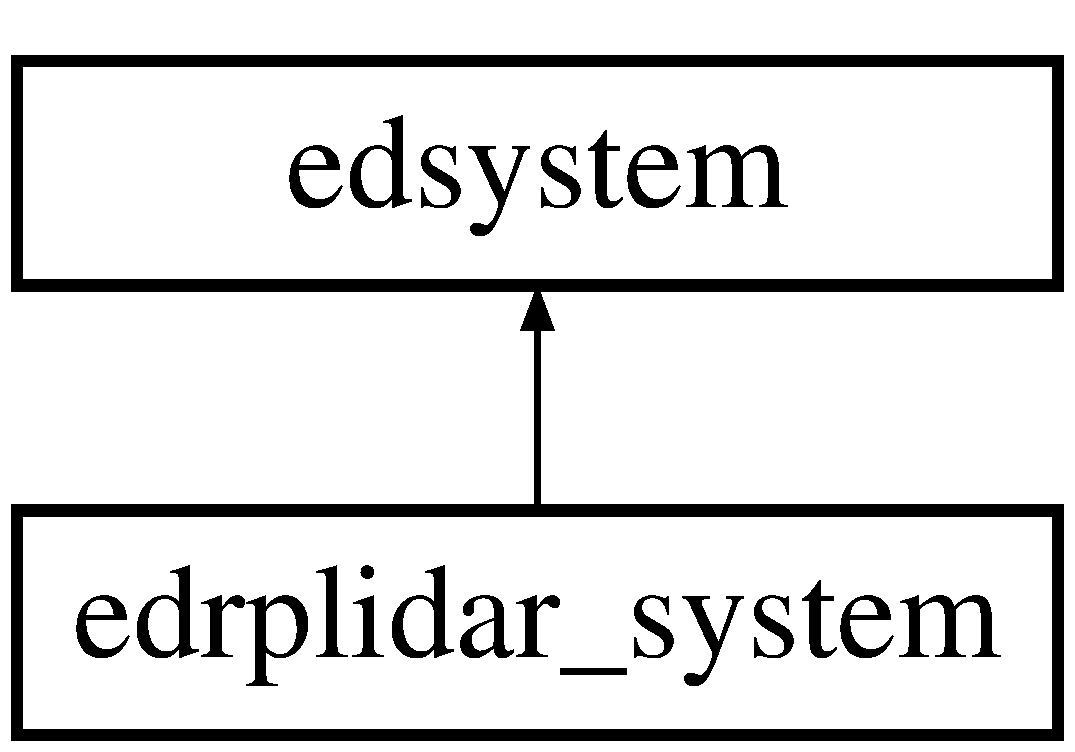
\includegraphics[height=2.000000cm]{classedrplidar__system}
\end{center}
\end{figure}
\subsection*{Public Types}
\begin{DoxyCompactItemize}
\item 
enum \hyperlink{classedrplidar__system_ab0690f6ca603a858d69080303761cd1f}{Exchange\-Type} \{ \\*
\hyperlink{classedrplidar__system_ab0690f6ca603a858d69080303761cd1fa869119dd4a3be62b03f4b5919bec0daf}{Scan}, 
\hyperlink{classedrplidar__system_ab0690f6ca603a858d69080303761cd1fab6bc43008cfd5ed1d2e5ba305efde764}{Info}, 
\hyperlink{classedrplidar__system_ab0690f6ca603a858d69080303761cd1fa32c68bd753b7cd05dc13ba9d0fdeb90f}{Health}, 
\hyperlink{classedrplidar__system_ab0690f6ca603a858d69080303761cd1fa01fc0219e454b92ab9e8c842bfa57d4a}{Reset}, 
\\*
\hyperlink{classedrplidar__system_ab0690f6ca603a858d69080303761cd1faf502cb7101cd1947fdd6c13bcd3f132c}{None}
 \}
\end{DoxyCompactItemize}
\subsection*{Public Member Functions}
\begin{DoxyCompactItemize}
\item 
\hyperlink{classedrplidar__system_a3189e92f56cd720a53f0c53c65f3fb53}{edrplidar\-\_\-system} ()
\item 
\hyperlink{classedrplidar__system_aab380eebadbfcd30ae16a4162ce17272}{$\sim$edrplidar\-\_\-system} ()
\item 
void \hyperlink{classedrplidar__system_aeac91046ef78f68cb9463ad216719def}{init} ()
\item 
void \hyperlink{classedrplidar__system_ab8e9f26bd1f1a8501b36d6eaedd44ced}{release} ()
\item 
bool \hyperlink{classedrplidar__system_aa6d1766212432f586944027b0d5b0950}{process} (\hyperlink{structedmessage}{edmessage} $\ast$msg)
\item 
void \hyperlink{classedrplidar__system_aeaa11dbbb634e7392629982a57868c62}{update} ()
\item 
std\-::string \hyperlink{classedrplidar__system_ae777072e4712d7bed997032842f2dad0}{typestr} ()
\end{DoxyCompactItemize}
\subsection*{Static Public Member Functions}
\begin{DoxyCompactItemize}
\item 
static std\-::string \hyperlink{classedrplidar__system_a8aae91a8f5522b8975617ad172c9f663}{Type\-String} ()
\end{DoxyCompactItemize}
\subsection*{Protected Member Functions}
\begin{DoxyCompactItemize}
\item 
bool \hyperlink{classedrplidar__system_a4780aae99366654694ac97e57b94ddbe}{start\-Scan} ()
\item 
bool \hyperlink{classedrplidar__system_aa4b0dcc8db62b695eaaa7f3f076d6958}{force\-Scan} ()
\item 
bool \hyperlink{classedrplidar__system_adb1b55f6f227dc7c1b8ea783be44aab5}{stop\-Scan} ()
\item 
bool \hyperlink{classedrplidar__system_abb48bf173a5590649f069b7340cdb110}{reset} ()
\item 
bool \hyperlink{classedrplidar__system_a35ce6a26a2d1370d7529953cc875cad3}{request\-Info} ()
\item 
bool \hyperlink{classedrplidar__system_aac73b78f69b44c15fdc168a5ed8543ee}{request\-Health} ()
\end{DoxyCompactItemize}


\subsection{Member Enumeration Documentation}
\hypertarget{classedrplidar__system_ab0690f6ca603a858d69080303761cd1f}{\index{edrplidar\-\_\-system@{edrplidar\-\_\-system}!Exchange\-Type@{Exchange\-Type}}
\index{Exchange\-Type@{Exchange\-Type}!edrplidar_system@{edrplidar\-\_\-system}}
\subsubsection[{Exchange\-Type}]{\setlength{\rightskip}{0pt plus 5cm}enum {\bf edrplidar\-\_\-system\-::\-Exchange\-Type}}}\label{classedrplidar__system_ab0690f6ca603a858d69080303761cd1f}
\begin{Desc}
\item[Enumerator]\par
\begin{description}
\index{Scan@{Scan}!edrplidar\-\_\-system@{edrplidar\-\_\-system}}\index{edrplidar\-\_\-system@{edrplidar\-\_\-system}!Scan@{Scan}}\item[{\em 
\hypertarget{classedrplidar__system_ab0690f6ca603a858d69080303761cd1fa869119dd4a3be62b03f4b5919bec0daf}{Scan}\label{classedrplidar__system_ab0690f6ca603a858d69080303761cd1fa869119dd4a3be62b03f4b5919bec0daf}
}]\index{Info@{Info}!edrplidar\-\_\-system@{edrplidar\-\_\-system}}\index{edrplidar\-\_\-system@{edrplidar\-\_\-system}!Info@{Info}}\item[{\em 
\hypertarget{classedrplidar__system_ab0690f6ca603a858d69080303761cd1fab6bc43008cfd5ed1d2e5ba305efde764}{Info}\label{classedrplidar__system_ab0690f6ca603a858d69080303761cd1fab6bc43008cfd5ed1d2e5ba305efde764}
}]\index{Health@{Health}!edrplidar\-\_\-system@{edrplidar\-\_\-system}}\index{edrplidar\-\_\-system@{edrplidar\-\_\-system}!Health@{Health}}\item[{\em 
\hypertarget{classedrplidar__system_ab0690f6ca603a858d69080303761cd1fa32c68bd753b7cd05dc13ba9d0fdeb90f}{Health}\label{classedrplidar__system_ab0690f6ca603a858d69080303761cd1fa32c68bd753b7cd05dc13ba9d0fdeb90f}
}]\index{Reset@{Reset}!edrplidar\-\_\-system@{edrplidar\-\_\-system}}\index{edrplidar\-\_\-system@{edrplidar\-\_\-system}!Reset@{Reset}}\item[{\em 
\hypertarget{classedrplidar__system_ab0690f6ca603a858d69080303761cd1fa01fc0219e454b92ab9e8c842bfa57d4a}{Reset}\label{classedrplidar__system_ab0690f6ca603a858d69080303761cd1fa01fc0219e454b92ab9e8c842bfa57d4a}
}]\index{None@{None}!edrplidar\-\_\-system@{edrplidar\-\_\-system}}\index{edrplidar\-\_\-system@{edrplidar\-\_\-system}!None@{None}}\item[{\em 
\hypertarget{classedrplidar__system_ab0690f6ca603a858d69080303761cd1faf502cb7101cd1947fdd6c13bcd3f132c}{None}\label{classedrplidar__system_ab0690f6ca603a858d69080303761cd1faf502cb7101cd1947fdd6c13bcd3f132c}
}]\end{description}
\end{Desc}


\subsection{Constructor \& Destructor Documentation}
\hypertarget{classedrplidar__system_a3189e92f56cd720a53f0c53c65f3fb53}{\index{edrplidar\-\_\-system@{edrplidar\-\_\-system}!edrplidar\-\_\-system@{edrplidar\-\_\-system}}
\index{edrplidar\-\_\-system@{edrplidar\-\_\-system}!edrplidar_system@{edrplidar\-\_\-system}}
\subsubsection[{edrplidar\-\_\-system}]{\setlength{\rightskip}{0pt plus 5cm}edrplidar\-\_\-system\-::edrplidar\-\_\-system (
\begin{DoxyParamCaption}
{}
\end{DoxyParamCaption}
)}}\label{classedrplidar__system_a3189e92f56cd720a53f0c53c65f3fb53}
\hypertarget{classedrplidar__system_aab380eebadbfcd30ae16a4162ce17272}{\index{edrplidar\-\_\-system@{edrplidar\-\_\-system}!$\sim$edrplidar\-\_\-system@{$\sim$edrplidar\-\_\-system}}
\index{$\sim$edrplidar\-\_\-system@{$\sim$edrplidar\-\_\-system}!edrplidar_system@{edrplidar\-\_\-system}}
\subsubsection[{$\sim$edrplidar\-\_\-system}]{\setlength{\rightskip}{0pt plus 5cm}edrplidar\-\_\-system\-::$\sim$edrplidar\-\_\-system (
\begin{DoxyParamCaption}
{}
\end{DoxyParamCaption}
)}}\label{classedrplidar__system_aab380eebadbfcd30ae16a4162ce17272}


\subsection{Member Function Documentation}
\hypertarget{classedrplidar__system_aa4b0dcc8db62b695eaaa7f3f076d6958}{\index{edrplidar\-\_\-system@{edrplidar\-\_\-system}!force\-Scan@{force\-Scan}}
\index{force\-Scan@{force\-Scan}!edrplidar_system@{edrplidar\-\_\-system}}
\subsubsection[{force\-Scan}]{\setlength{\rightskip}{0pt plus 5cm}bool edrplidar\-\_\-system\-::force\-Scan (
\begin{DoxyParamCaption}
{}
\end{DoxyParamCaption}
)\hspace{0.3cm}{\ttfamily [protected]}}}\label{classedrplidar__system_aa4b0dcc8db62b695eaaa7f3f076d6958}
\hypertarget{classedrplidar__system_aeac91046ef78f68cb9463ad216719def}{\index{edrplidar\-\_\-system@{edrplidar\-\_\-system}!init@{init}}
\index{init@{init}!edrplidar_system@{edrplidar\-\_\-system}}
\subsubsection[{init}]{\setlength{\rightskip}{0pt plus 5cm}void edrplidar\-\_\-system\-::init (
\begin{DoxyParamCaption}
{}
\end{DoxyParamCaption}
)\hspace{0.3cm}{\ttfamily [virtual]}}}\label{classedrplidar__system_aeac91046ef78f68cb9463ad216719def}


Implements \hyperlink{classedsystem_a4c70e3568064941607fb220aea826a56}{edsystem}.

\hypertarget{classedrplidar__system_aa6d1766212432f586944027b0d5b0950}{\index{edrplidar\-\_\-system@{edrplidar\-\_\-system}!process@{process}}
\index{process@{process}!edrplidar_system@{edrplidar\-\_\-system}}
\subsubsection[{process}]{\setlength{\rightskip}{0pt plus 5cm}bool edrplidar\-\_\-system\-::process (
\begin{DoxyParamCaption}
\item[{{\bf edmessage} $\ast$}]{msg}
\end{DoxyParamCaption}
)\hspace{0.3cm}{\ttfamily [virtual]}}}\label{classedrplidar__system_aa6d1766212432f586944027b0d5b0950}


Implements \hyperlink{classedsystem_a9d7a0547c702af1572ed8a1f5434fa0a}{edsystem}.

\hypertarget{classedrplidar__system_ab8e9f26bd1f1a8501b36d6eaedd44ced}{\index{edrplidar\-\_\-system@{edrplidar\-\_\-system}!release@{release}}
\index{release@{release}!edrplidar_system@{edrplidar\-\_\-system}}
\subsubsection[{release}]{\setlength{\rightskip}{0pt plus 5cm}void edrplidar\-\_\-system\-::release (
\begin{DoxyParamCaption}
{}
\end{DoxyParamCaption}
)\hspace{0.3cm}{\ttfamily [virtual]}}}\label{classedrplidar__system_ab8e9f26bd1f1a8501b36d6eaedd44ced}


Implements \hyperlink{classedsystem_af40ac185ca4a8efd6777fdb4c65880ea}{edsystem}.

\hypertarget{classedrplidar__system_aac73b78f69b44c15fdc168a5ed8543ee}{\index{edrplidar\-\_\-system@{edrplidar\-\_\-system}!request\-Health@{request\-Health}}
\index{request\-Health@{request\-Health}!edrplidar_system@{edrplidar\-\_\-system}}
\subsubsection[{request\-Health}]{\setlength{\rightskip}{0pt plus 5cm}bool edrplidar\-\_\-system\-::request\-Health (
\begin{DoxyParamCaption}
{}
\end{DoxyParamCaption}
)\hspace{0.3cm}{\ttfamily [protected]}}}\label{classedrplidar__system_aac73b78f69b44c15fdc168a5ed8543ee}
\hypertarget{classedrplidar__system_a35ce6a26a2d1370d7529953cc875cad3}{\index{edrplidar\-\_\-system@{edrplidar\-\_\-system}!request\-Info@{request\-Info}}
\index{request\-Info@{request\-Info}!edrplidar_system@{edrplidar\-\_\-system}}
\subsubsection[{request\-Info}]{\setlength{\rightskip}{0pt plus 5cm}bool edrplidar\-\_\-system\-::request\-Info (
\begin{DoxyParamCaption}
{}
\end{DoxyParamCaption}
)\hspace{0.3cm}{\ttfamily [protected]}}}\label{classedrplidar__system_a35ce6a26a2d1370d7529953cc875cad3}
\hypertarget{classedrplidar__system_abb48bf173a5590649f069b7340cdb110}{\index{edrplidar\-\_\-system@{edrplidar\-\_\-system}!reset@{reset}}
\index{reset@{reset}!edrplidar_system@{edrplidar\-\_\-system}}
\subsubsection[{reset}]{\setlength{\rightskip}{0pt plus 5cm}bool edrplidar\-\_\-system\-::reset (
\begin{DoxyParamCaption}
{}
\end{DoxyParamCaption}
)\hspace{0.3cm}{\ttfamily [protected]}}}\label{classedrplidar__system_abb48bf173a5590649f069b7340cdb110}
\hypertarget{classedrplidar__system_a4780aae99366654694ac97e57b94ddbe}{\index{edrplidar\-\_\-system@{edrplidar\-\_\-system}!start\-Scan@{start\-Scan}}
\index{start\-Scan@{start\-Scan}!edrplidar_system@{edrplidar\-\_\-system}}
\subsubsection[{start\-Scan}]{\setlength{\rightskip}{0pt plus 5cm}bool edrplidar\-\_\-system\-::start\-Scan (
\begin{DoxyParamCaption}
{}
\end{DoxyParamCaption}
)\hspace{0.3cm}{\ttfamily [protected]}}}\label{classedrplidar__system_a4780aae99366654694ac97e57b94ddbe}
\hypertarget{classedrplidar__system_adb1b55f6f227dc7c1b8ea783be44aab5}{\index{edrplidar\-\_\-system@{edrplidar\-\_\-system}!stop\-Scan@{stop\-Scan}}
\index{stop\-Scan@{stop\-Scan}!edrplidar_system@{edrplidar\-\_\-system}}
\subsubsection[{stop\-Scan}]{\setlength{\rightskip}{0pt plus 5cm}bool edrplidar\-\_\-system\-::stop\-Scan (
\begin{DoxyParamCaption}
{}
\end{DoxyParamCaption}
)\hspace{0.3cm}{\ttfamily [protected]}}}\label{classedrplidar__system_adb1b55f6f227dc7c1b8ea783be44aab5}
\hypertarget{classedrplidar__system_ae777072e4712d7bed997032842f2dad0}{\index{edrplidar\-\_\-system@{edrplidar\-\_\-system}!typestr@{typestr}}
\index{typestr@{typestr}!edrplidar_system@{edrplidar\-\_\-system}}
\subsubsection[{typestr}]{\setlength{\rightskip}{0pt plus 5cm}std\-::string edrplidar\-\_\-system\-::typestr (
\begin{DoxyParamCaption}
{}
\end{DoxyParamCaption}
)\hspace{0.3cm}{\ttfamily [inline]}, {\ttfamily [virtual]}}}\label{classedrplidar__system_ae777072e4712d7bed997032842f2dad0}


Implements \hyperlink{classedsystem_a19dc65111f9a38259fcafba3a32a646d}{edsystem}.

\hypertarget{classedrplidar__system_a8aae91a8f5522b8975617ad172c9f663}{\index{edrplidar\-\_\-system@{edrplidar\-\_\-system}!Type\-String@{Type\-String}}
\index{Type\-String@{Type\-String}!edrplidar_system@{edrplidar\-\_\-system}}
\subsubsection[{Type\-String}]{\setlength{\rightskip}{0pt plus 5cm}static std\-::string edrplidar\-\_\-system\-::\-Type\-String (
\begin{DoxyParamCaption}
{}
\end{DoxyParamCaption}
)\hspace{0.3cm}{\ttfamily [inline]}, {\ttfamily [static]}}}\label{classedrplidar__system_a8aae91a8f5522b8975617ad172c9f663}
\hypertarget{classedrplidar__system_aeaa11dbbb634e7392629982a57868c62}{\index{edrplidar\-\_\-system@{edrplidar\-\_\-system}!update@{update}}
\index{update@{update}!edrplidar_system@{edrplidar\-\_\-system}}
\subsubsection[{update}]{\setlength{\rightskip}{0pt plus 5cm}void edrplidar\-\_\-system\-::update (
\begin{DoxyParamCaption}
{}
\end{DoxyParamCaption}
)\hspace{0.3cm}{\ttfamily [virtual]}}}\label{classedrplidar__system_aeaa11dbbb634e7392629982a57868c62}


Implements \hyperlink{classedsystem_afd5308dc71350fe4e239cac5fb1bdbe9}{edsystem}.



The documentation for this class was generated from the following files\-:\begin{DoxyCompactItemize}
\item 
/home/dprandle/\-Documents/code/ctrlmod/include/\hyperlink{edrplidar__system_8h}{edrplidar\-\_\-system.\-h}\item 
/home/dprandle/\-Documents/code/ctrlmod/src/\hyperlink{edrplidar__system_8cpp}{edrplidar\-\_\-system.\-cpp}\end{DoxyCompactItemize}

\hypertarget{classedsocket}{\section{edsocket Class Reference}
\label{classedsocket}\index{edsocket@{edsocket}}
}


{\ttfamily \#include $<$edsocket.\-h$>$}

Inheritance diagram for edsocket\-:\begin{figure}[H]
\begin{center}
\leavevmode
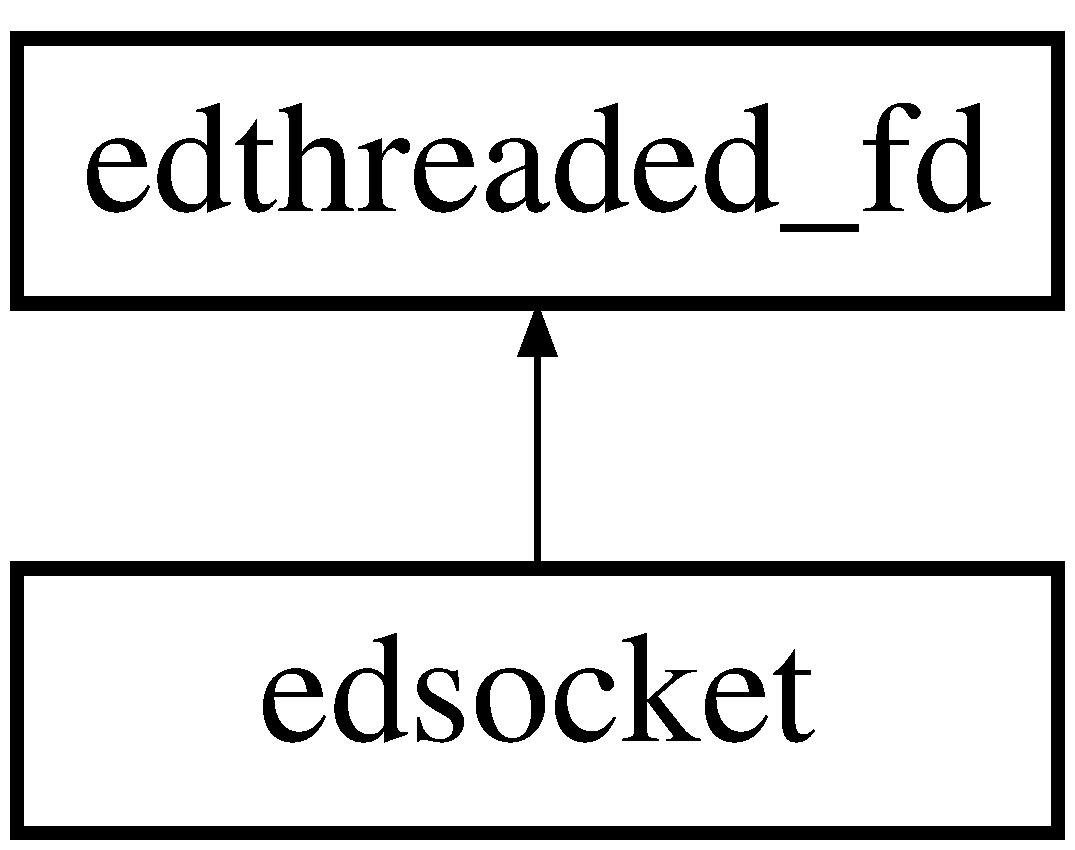
\includegraphics[height=2.000000cm]{classedsocket}
\end{center}
\end{figure}
\subsection*{Public Member Functions}
\begin{DoxyCompactItemize}
\item 
\hyperlink{classedsocket_ac3ad6e1e73a61627ee30a35d5e3423d1}{edsocket} (uint32\-\_\-t socket\-\_\-fd)
\item 
\hyperlink{classedsocket_abdf101da378e31165dfcddfd6e6c9177}{$\sim$edsocket} ()
\end{DoxyCompactItemize}
\subsection*{Additional Inherited Members}


\subsection{Constructor \& Destructor Documentation}
\hypertarget{classedsocket_ac3ad6e1e73a61627ee30a35d5e3423d1}{\index{edsocket@{edsocket}!edsocket@{edsocket}}
\index{edsocket@{edsocket}!edsocket@{edsocket}}
\subsubsection[{edsocket}]{\setlength{\rightskip}{0pt plus 5cm}edsocket\-::edsocket (
\begin{DoxyParamCaption}
\item[{uint32\-\_\-t}]{socket\-\_\-fd}
\end{DoxyParamCaption}
)}}\label{classedsocket_ac3ad6e1e73a61627ee30a35d5e3423d1}
\hypertarget{classedsocket_abdf101da378e31165dfcddfd6e6c9177}{\index{edsocket@{edsocket}!$\sim$edsocket@{$\sim$edsocket}}
\index{$\sim$edsocket@{$\sim$edsocket}!edsocket@{edsocket}}
\subsubsection[{$\sim$edsocket}]{\setlength{\rightskip}{0pt plus 5cm}edsocket\-::$\sim$edsocket (
\begin{DoxyParamCaption}
{}
\end{DoxyParamCaption}
)}}\label{classedsocket_abdf101da378e31165dfcddfd6e6c9177}


The documentation for this class was generated from the following files\-:\begin{DoxyCompactItemize}
\item 
/home/dprandle/\-Documents/code/ctrlmod/include/\hyperlink{edsocket_8h}{edsocket.\-h}\item 
/home/dprandle/\-Documents/code/ctrlmod/src/\hyperlink{edsocket_8cpp}{edsocket.\-cpp}\end{DoxyCompactItemize}

\hypertarget{classedsystem}{\section{edsystem Class Reference}
\label{classedsystem}\index{edsystem@{edsystem}}
}


{\ttfamily \#include $<$edsystem.\-h$>$}

Inheritance diagram for edsystem\-:\begin{figure}[H]
\begin{center}
\leavevmode
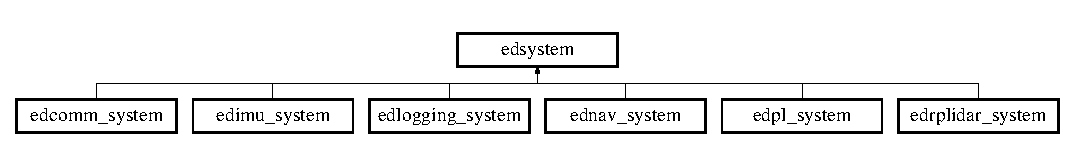
\includegraphics[height=1.555556cm]{classedsystem}
\end{center}
\end{figure}
\subsection*{Public Member Functions}
\begin{DoxyCompactItemize}
\item 
\hyperlink{classedsystem_af87c5a01f7cf70dcc788bbf1dbd8aeb1}{edsystem} ()
\item 
virtual \hyperlink{classedsystem_af3022d068ee9dda5b7da8438680e6437}{$\sim$edsystem} ()
\item 
virtual void \hyperlink{classedsystem_a4c70e3568064941607fb220aea826a56}{init} ()=0
\item 
virtual void \hyperlink{classedsystem_af40ac185ca4a8efd6777fdb4c65880ea}{release} ()=0
\item 
virtual bool \hyperlink{classedsystem_a9d7a0547c702af1572ed8a1f5434fa0a}{process} (\hyperlink{structedmessage}{edmessage} $\ast$msg)=0
\item 
virtual void \hyperlink{classedsystem_afd5308dc71350fe4e239cac5fb1bdbe9}{update} ()=0
\item 
virtual std\-::string \hyperlink{classedsystem_a19dc65111f9a38259fcafba3a32a646d}{typestr} ()=0
\end{DoxyCompactItemize}


\subsection{Constructor \& Destructor Documentation}
\hypertarget{classedsystem_af87c5a01f7cf70dcc788bbf1dbd8aeb1}{\index{edsystem@{edsystem}!edsystem@{edsystem}}
\index{edsystem@{edsystem}!edsystem@{edsystem}}
\subsubsection[{edsystem}]{\setlength{\rightskip}{0pt plus 5cm}edsystem\-::edsystem (
\begin{DoxyParamCaption}
{}
\end{DoxyParamCaption}
)\hspace{0.3cm}{\ttfamily [inline]}}}\label{classedsystem_af87c5a01f7cf70dcc788bbf1dbd8aeb1}
\hypertarget{classedsystem_af3022d068ee9dda5b7da8438680e6437}{\index{edsystem@{edsystem}!$\sim$edsystem@{$\sim$edsystem}}
\index{$\sim$edsystem@{$\sim$edsystem}!edsystem@{edsystem}}
\subsubsection[{$\sim$edsystem}]{\setlength{\rightskip}{0pt plus 5cm}virtual edsystem\-::$\sim$edsystem (
\begin{DoxyParamCaption}
{}
\end{DoxyParamCaption}
)\hspace{0.3cm}{\ttfamily [inline]}, {\ttfamily [virtual]}}}\label{classedsystem_af3022d068ee9dda5b7da8438680e6437}


\subsection{Member Function Documentation}
\hypertarget{classedsystem_a4c70e3568064941607fb220aea826a56}{\index{edsystem@{edsystem}!init@{init}}
\index{init@{init}!edsystem@{edsystem}}
\subsubsection[{init}]{\setlength{\rightskip}{0pt plus 5cm}virtual void edsystem\-::init (
\begin{DoxyParamCaption}
{}
\end{DoxyParamCaption}
)\hspace{0.3cm}{\ttfamily [pure virtual]}}}\label{classedsystem_a4c70e3568064941607fb220aea826a56}


Implemented in \hyperlink{classedimu__system_af745d305e5ff1cfaba3134fd4ff2c342}{edimu\-\_\-system}, \hyperlink{classedpl__system_a4d9fae9e10da9cae1f1e7a00e751c933}{edpl\-\_\-system}, \hyperlink{classednav__system_a98bc9b1cecf79a6ca7145e34a0273ca2}{ednav\-\_\-system}, \hyperlink{classedcomm__system_a07f81f18aeca00b88928a8aec7b3129e}{edcomm\-\_\-system}, \hyperlink{classedrplidar__system_aeac91046ef78f68cb9463ad216719def}{edrplidar\-\_\-system}, and \hyperlink{classedlogging__system_a393094d06bb5d15155be58286f0a5185}{edlogging\-\_\-system}.

\hypertarget{classedsystem_a9d7a0547c702af1572ed8a1f5434fa0a}{\index{edsystem@{edsystem}!process@{process}}
\index{process@{process}!edsystem@{edsystem}}
\subsubsection[{process}]{\setlength{\rightskip}{0pt plus 5cm}virtual bool edsystem\-::process (
\begin{DoxyParamCaption}
\item[{{\bf edmessage} $\ast$}]{msg}
\end{DoxyParamCaption}
)\hspace{0.3cm}{\ttfamily [pure virtual]}}}\label{classedsystem_a9d7a0547c702af1572ed8a1f5434fa0a}


Implemented in \hyperlink{classedimu__system_abd6e59b943adbb48fa786f10f809070c}{edimu\-\_\-system}, \hyperlink{classedpl__system_a4aae16b8695eec7c54ccfaecee9c535c}{edpl\-\_\-system}, \hyperlink{classednav__system_ae90088e1c3a01fdeb0fc051af71e6d6a}{ednav\-\_\-system}, \hyperlink{classedcomm__system_ad3b79f16dd77b5ae458cc360550e99cd}{edcomm\-\_\-system}, \hyperlink{classedrplidar__system_aa6d1766212432f586944027b0d5b0950}{edrplidar\-\_\-system}, and \hyperlink{classedlogging__system_aa1d63881863c61a89e80aa8187b8d19d}{edlogging\-\_\-system}.

\hypertarget{classedsystem_af40ac185ca4a8efd6777fdb4c65880ea}{\index{edsystem@{edsystem}!release@{release}}
\index{release@{release}!edsystem@{edsystem}}
\subsubsection[{release}]{\setlength{\rightskip}{0pt plus 5cm}virtual void edsystem\-::release (
\begin{DoxyParamCaption}
{}
\end{DoxyParamCaption}
)\hspace{0.3cm}{\ttfamily [pure virtual]}}}\label{classedsystem_af40ac185ca4a8efd6777fdb4c65880ea}


Implemented in \hyperlink{classedimu__system_a65927db96dc88e8752f0529d9faa6bc0}{edimu\-\_\-system}, \hyperlink{classedpl__system_adb2b906b466251dc513fb9d669a19e99}{edpl\-\_\-system}, \hyperlink{classednav__system_aa41383e31657188e5386b45d4dd7e4cd}{ednav\-\_\-system}, \hyperlink{classedcomm__system_ad9bdfd2845a3156f5d010e99f8fbed07}{edcomm\-\_\-system}, \hyperlink{classedrplidar__system_ab8e9f26bd1f1a8501b36d6eaedd44ced}{edrplidar\-\_\-system}, and \hyperlink{classedlogging__system_ad959e6d140397e22953b2b7d1738456a}{edlogging\-\_\-system}.

\hypertarget{classedsystem_a19dc65111f9a38259fcafba3a32a646d}{\index{edsystem@{edsystem}!typestr@{typestr}}
\index{typestr@{typestr}!edsystem@{edsystem}}
\subsubsection[{typestr}]{\setlength{\rightskip}{0pt plus 5cm}virtual std\-::string edsystem\-::typestr (
\begin{DoxyParamCaption}
{}
\end{DoxyParamCaption}
)\hspace{0.3cm}{\ttfamily [pure virtual]}}}\label{classedsystem_a19dc65111f9a38259fcafba3a32a646d}


Implemented in \hyperlink{classedimu__system_ae3124c577ae10d92f69438f28ce67969}{edimu\-\_\-system}, \hyperlink{classedpl__system_ab758bc4300926af08e47e0c8b655d8fc}{edpl\-\_\-system}, \hyperlink{classedcomm__system_a61e1243fba536c8263ba93367cd5a2a7}{edcomm\-\_\-system}, \hyperlink{classednav__system_a3d604cf5dcff8c1c7d8c492e213c1e3c}{ednav\-\_\-system}, \hyperlink{classedrplidar__system_ae777072e4712d7bed997032842f2dad0}{edrplidar\-\_\-system}, and \hyperlink{classedlogging__system_ad1262db654a7d7acee6b217a09588170}{edlogging\-\_\-system}.

\hypertarget{classedsystem_afd5308dc71350fe4e239cac5fb1bdbe9}{\index{edsystem@{edsystem}!update@{update}}
\index{update@{update}!edsystem@{edsystem}}
\subsubsection[{update}]{\setlength{\rightskip}{0pt plus 5cm}virtual void edsystem\-::update (
\begin{DoxyParamCaption}
{}
\end{DoxyParamCaption}
)\hspace{0.3cm}{\ttfamily [pure virtual]}}}\label{classedsystem_afd5308dc71350fe4e239cac5fb1bdbe9}


Implemented in \hyperlink{classedimu__system_a70926a3b36b53f54913fc47ee471fb9b}{edimu\-\_\-system}, \hyperlink{classedpl__system_ae84af8dea7c53fe3219e7cde15ddd43a}{edpl\-\_\-system}, \hyperlink{classednav__system_a3a32c9f0ee4c089ac2e0eff9dae9a879}{ednav\-\_\-system}, \hyperlink{classedcomm__system_adc9ffc8199070ad0d836a447005a4e1e}{edcomm\-\_\-system}, \hyperlink{classedrplidar__system_aeaa11dbbb634e7392629982a57868c62}{edrplidar\-\_\-system}, and \hyperlink{classedlogging__system_ac9b9dd8d391244acdea02666a56f8440}{edlogging\-\_\-system}.



The documentation for this class was generated from the following file\-:\begin{DoxyCompactItemize}
\item 
/home/dprandle/\-Documents/code/ctrlmod/include/\hyperlink{edsystem_8h}{edsystem.\-h}\end{DoxyCompactItemize}

\hypertarget{classedthreaded__fd}{\section{edthreaded\-\_\-fd Class Reference}
\label{classedthreaded__fd}\index{edthreaded\-\_\-fd@{edthreaded\-\_\-fd}}
}


{\ttfamily \#include $<$edthreaded\-\_\-fd.\-h$>$}

Inheritance diagram for edthreaded\-\_\-fd\-:\begin{figure}[H]
\begin{center}
\leavevmode
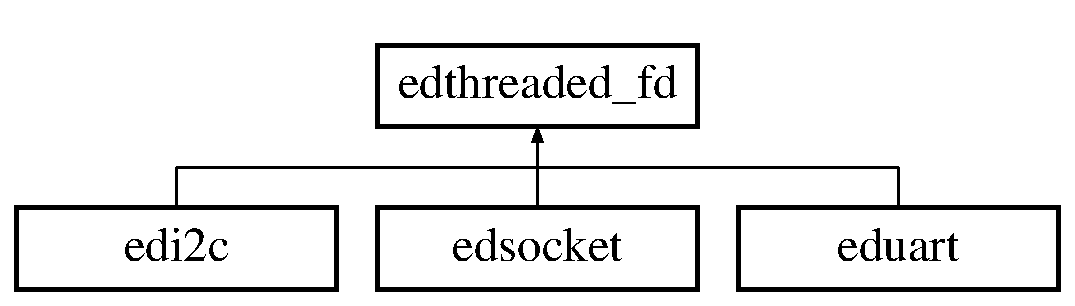
\includegraphics[height=2.000000cm]{classedthreaded__fd}
\end{center}
\end{figure}
\subsection*{Classes}
\begin{DoxyCompactItemize}
\item 
struct \hyperlink{structedthreaded__fd_1_1Error}{Error}
\item 
struct \hyperlink{structedthreaded__fd_1_1WriteVal}{Write\-Val}
\end{DoxyCompactItemize}
\subsection*{Public Types}
\begin{DoxyCompactItemize}
\item 
enum \hyperlink{classedthreaded__fd_ab3562872429271887a15489b7a1a17d7}{Error\-Val} \{ \\*
\hyperlink{classedthreaded__fd_ab3562872429271887a15489b7a1a17d7a29beb6d1cc1d22cc04de457e10c9ca35}{No\-Error}, 
\hyperlink{classedthreaded__fd_ab3562872429271887a15489b7a1a17d7ae07e73e070b49478688e0d9f77b58b55}{Connection\-Closed}, 
\hyperlink{classedthreaded__fd_ab3562872429271887a15489b7a1a17d7a02dc57182bb3c610c739d52417ba5359}{Data\-Overwrite}, 
\hyperlink{classedthreaded__fd_ab3562872429271887a15489b7a1a17d7af16a08099723c4d84dc0c4799d1ff864}{Invalid\-Read}, 
\\*
\hyperlink{classedthreaded__fd_ab3562872429271887a15489b7a1a17d7a40d6cb36b60a22ded9e067b54c85a305}{Invalid\-Write}, 
\hyperlink{classedthreaded__fd_ab3562872429271887a15489b7a1a17d7af129b616b31507425750a425e7952fff}{Thread\-Creation}, 
\hyperlink{classedthreaded__fd_ab3562872429271887a15489b7a1a17d7a4abb816be001c2c4b8ff3a4092ab048d}{Open\-File\-Descriptor}, 
\hyperlink{classedthreaded__fd_ab3562872429271887a15489b7a1a17d7aa99856ec175ebaa60bd324b58aa2c3dc}{Configuration}, 
\\*
\hyperlink{classedthreaded__fd_ab3562872429271887a15489b7a1a17d7af195ec5ad8131af045485af5b04c4131}{Already\-Running}, 
\hyperlink{classedthreaded__fd_ab3562872429271887a15489b7a1a17d7aac2ebbfb6e21042eb50ca713a1b5e394}{F\-D\-Already\-Open}, 
\hyperlink{classedthreaded__fd_ab3562872429271887a15489b7a1a17d7a2ef2a2f6fd755b520613dbaa22f26396}{Command\-No\-Response}
 \}
\end{DoxyCompactItemize}
\subsection*{Public Member Functions}
\begin{DoxyCompactItemize}
\item 
\hyperlink{classedthreaded__fd_aae0e03e726a962766ada1a053e426dfc}{edthreaded\-\_\-fd} (uint32\-\_\-t readbuf\-\_\-size=\hyperlink{edthreaded__fd_8h_a645b973029e4897854f96c850e30eaa3}{D\-E\-F\-A\-U\-L\-T\-\_\-\-F\-D\-\_\-\-R\-E\-A\-D\-\_\-\-B\-U\-F\-F\-E\-R\-\_\-\-S\-I\-Z\-E}, uint32\-\_\-t writebuf\-\_\-size=\hyperlink{edthreaded__fd_8h_a342873b4069f62ee07236e149ab6471b}{D\-E\-F\-A\-U\-L\-T\-\_\-\-F\-D\-\_\-\-W\-R\-I\-T\-E\-\_\-\-B\-U\-F\-F\-E\-R\-\_\-\-S\-I\-Z\-E})
\item 
virtual \hyperlink{classedthreaded__fd_a6f9a9d65186740a24d9bd3f164034e39}{$\sim$edthreaded\-\_\-fd} ()
\item 
virtual uint32\-\_\-t \hyperlink{classedthreaded__fd_a8f5b6c664a8fe5df737222e225f1fd19}{read} (uint8\-\_\-t $\ast$buffer, uint32\-\_\-t max\-\_\-size)
\item 
virtual uint32\-\_\-t \hyperlink{classedthreaded__fd_a69c6badd6cf1a9a635d670d2afec80d3}{write} (uint8\-\_\-t $\ast$buffer, uint32\-\_\-t size, int32\-\_\-t response\-\_\-size=0)
\item 
virtual \hyperlink{structedthreaded__fd_1_1Error}{Error} \hyperlink{classedthreaded__fd_a3708a6fecec91ca541a1c1c834bec7dd}{error} ()
\item 
bool \hyperlink{classedthreaded__fd_a55493d7c23181335e8412e2e7874795b}{running} ()
\item 
virtual bool \hyperlink{classedthreaded__fd_ac8123803d831c671b9b62881697e69e0}{start} ()
\item 
int32\-\_\-t \hyperlink{classedthreaded__fd_a4b4e4f3c1e8c0a4fd5389bcb8690ef08}{fd} ()
\item 
bool \hyperlink{classedthreaded__fd_aadead96bf63b16f95c48c7a863323b0e}{set\-\_\-fd} (int32\-\_\-t fd\-\_\-)
\item 
virtual void \hyperlink{classedthreaded__fd_a92a9a1f5b8df83c5697033822f1134b8}{stop} ()
\end{DoxyCompactItemize}
\subsection*{Protected Member Functions}
\begin{DoxyCompactItemize}
\item 
virtual int32\-\_\-t \hyperlink{classedthreaded__fd_a3ead513fc5aa5b33e18a6b7246091ee9}{\-\_\-raw\-\_\-read} (uint8\-\_\-t $\ast$buffer, uint32\-\_\-t max\-\_\-size)=0
\item 
virtual int32\-\_\-t \hyperlink{classedthreaded__fd_a0151298dfd0c91b95d27649031c5fa53}{\-\_\-raw\-\_\-write} (uint8\-\_\-t $\ast$buffer, uint32\-\_\-t max\-\_\-size)=0
\item 
virtual void \hyperlink{classedthreaded__fd_a251c391b913e2c151eb8840773f505c0}{\-\_\-do\-\_\-read} ()
\item 
virtual void \hyperlink{classedthreaded__fd_a0f6def6ed7b6147aad0f7007bcff83ee}{\-\_\-do\-\_\-write} ()
\item 
virtual void \hyperlink{classedthreaded__fd_a42c7b3bc22648ebbc71a1daeb1ac2535}{\-\_\-exec} ()
\item 
void \hyperlink{classedthreaded__fd_acf2f0e638887933b62229bf543c8733d}{\-\_\-set\-Error} (\hyperlink{classedthreaded__fd_ab3562872429271887a15489b7a1a17d7}{Error\-Val} err\-\_\-val, int32\-\_\-t \-\_\-errno)
\end{DoxyCompactItemize}
\subsection*{Static Protected Member Functions}
\begin{DoxyCompactItemize}
\item 
static void $\ast$ \hyperlink{classedthreaded__fd_a7fbc6179a5ea6829529d01c94a659053}{thread\-\_\-exec} (void $\ast$)
\end{DoxyCompactItemize}
\subsection*{Protected Attributes}
\begin{DoxyCompactItemize}
\item 
int32\-\_\-t \hyperlink{classedthreaded__fd_aec9e15343d8764eae71949abfb72aae6}{m\-\_\-fd}
\item 
uint32\-\_\-t \hyperlink{classedthreaded__fd_a0b15523ca598761128ac79f7f4864d72}{m\-\_\-read\-\_\-rawindex}
\item 
uint32\-\_\-t \hyperlink{classedthreaded__fd_a4ada8ce6e55d793e5ac35fef6069cac2}{m\-\_\-read\-\_\-curindex}
\item 
uint32\-\_\-t \hyperlink{classedthreaded__fd_a5e31d54e745a41467270d2e8facef9f6}{m\-\_\-write\-\_\-rawindex}
\item 
uint32\-\_\-t \hyperlink{classedthreaded__fd_a318812ed9af58952dc87849634145e91}{m\-\_\-write\-\_\-curindex}
\item 
std\-::vector$<$ \hyperlink{structedthreaded__fd_1_1WriteVal}{Write\-Val} $>$ \hyperlink{classedthreaded__fd_aeaba4592ba02680a1d8653479f0d1d87}{m\-\_\-write\-\_\-buffer}
\item 
std\-::vector$<$ uint8\-\_\-t $>$ \hyperlink{classedthreaded__fd_ae1b93e783eee5006dd652cf75c117f28}{m\-\_\-read\-\_\-buffer}
\item 
\hyperlink{structedthreaded__fd_1_1Error}{Error} \hyperlink{classedthreaded__fd_a74eb86ee72a5dfa499e0529ac59955b0}{m\-\_\-err}
\item 
bool \hyperlink{classedthreaded__fd_a7ee685acbb7cb287455311b2dcd09bd4}{m\-\_\-running}
\item 
uint32\-\_\-t \hyperlink{classedthreaded__fd_a42482e8096aed090ead1f08f049a24e6}{m\-\_\-current\-\_\-wait\-\_\-for\-\_\-byte\-\_\-count}
\item 
\hyperlink{classedtimer}{edtimer} $\ast$ \hyperlink{classedthreaded__fd_ae1244377b4ee3faf7f4cb9e21afadba6}{m\-\_\-wait\-\_\-timer}
\item 
pthread\-\_\-mutex\-\_\-t \hyperlink{classedthreaded__fd_a8614fe087b0c94cc56be6b3cd71dbd66}{m\-\_\-send\-\_\-lock}
\item 
pthread\-\_\-mutex\-\_\-t \hyperlink{classedthreaded__fd_a9c2f74e0cd623edc946b6bd74de87e24}{m\-\_\-recv\-\_\-lock}
\item 
pthread\-\_\-mutex\-\_\-t \hyperlink{classedthreaded__fd_a407c7283668e38cefb828a3f4f4ec117}{m\-\_\-error\-\_\-lock}
\item 
pthread\-\_\-mutex\-\_\-t \hyperlink{classedthreaded__fd_a44b98e3c701b2b71b7abee958b05c1d8}{m\-\_\-running\-\_\-lock}
\item 
pthread\-\_\-t \hyperlink{classedthreaded__fd_a96c9e8af500d47320c1396cc270cc41e}{m\-\_\-thread}
\end{DoxyCompactItemize}
\subsection*{Friends}
\begin{DoxyCompactItemize}
\item 
struct \hyperlink{classedthreaded__fd_a51b319f0e7d155dc96111998cbf641e2}{command\-\_\-wait\-\_\-callback}
\end{DoxyCompactItemize}


\subsection{Member Enumeration Documentation}
\hypertarget{classedthreaded__fd_ab3562872429271887a15489b7a1a17d7}{\index{edthreaded\-\_\-fd@{edthreaded\-\_\-fd}!Error\-Val@{Error\-Val}}
\index{Error\-Val@{Error\-Val}!edthreaded_fd@{edthreaded\-\_\-fd}}
\subsubsection[{Error\-Val}]{\setlength{\rightskip}{0pt plus 5cm}enum {\bf edthreaded\-\_\-fd\-::\-Error\-Val}}}\label{classedthreaded__fd_ab3562872429271887a15489b7a1a17d7}
\begin{Desc}
\item[Enumerator]\par
\begin{description}
\index{No\-Error@{No\-Error}!edthreaded\-\_\-fd@{edthreaded\-\_\-fd}}\index{edthreaded\-\_\-fd@{edthreaded\-\_\-fd}!No\-Error@{No\-Error}}\item[{\em 
\hypertarget{classedthreaded__fd_ab3562872429271887a15489b7a1a17d7a29beb6d1cc1d22cc04de457e10c9ca35}{No\-Error}\label{classedthreaded__fd_ab3562872429271887a15489b7a1a17d7a29beb6d1cc1d22cc04de457e10c9ca35}
}]\index{Connection\-Closed@{Connection\-Closed}!edthreaded\-\_\-fd@{edthreaded\-\_\-fd}}\index{edthreaded\-\_\-fd@{edthreaded\-\_\-fd}!Connection\-Closed@{Connection\-Closed}}\item[{\em 
\hypertarget{classedthreaded__fd_ab3562872429271887a15489b7a1a17d7ae07e73e070b49478688e0d9f77b58b55}{Connection\-Closed}\label{classedthreaded__fd_ab3562872429271887a15489b7a1a17d7ae07e73e070b49478688e0d9f77b58b55}
}]\index{Data\-Overwrite@{Data\-Overwrite}!edthreaded\-\_\-fd@{edthreaded\-\_\-fd}}\index{edthreaded\-\_\-fd@{edthreaded\-\_\-fd}!Data\-Overwrite@{Data\-Overwrite}}\item[{\em 
\hypertarget{classedthreaded__fd_ab3562872429271887a15489b7a1a17d7a02dc57182bb3c610c739d52417ba5359}{Data\-Overwrite}\label{classedthreaded__fd_ab3562872429271887a15489b7a1a17d7a02dc57182bb3c610c739d52417ba5359}
}]\index{Invalid\-Read@{Invalid\-Read}!edthreaded\-\_\-fd@{edthreaded\-\_\-fd}}\index{edthreaded\-\_\-fd@{edthreaded\-\_\-fd}!Invalid\-Read@{Invalid\-Read}}\item[{\em 
\hypertarget{classedthreaded__fd_ab3562872429271887a15489b7a1a17d7af16a08099723c4d84dc0c4799d1ff864}{Invalid\-Read}\label{classedthreaded__fd_ab3562872429271887a15489b7a1a17d7af16a08099723c4d84dc0c4799d1ff864}
}]\index{Invalid\-Write@{Invalid\-Write}!edthreaded\-\_\-fd@{edthreaded\-\_\-fd}}\index{edthreaded\-\_\-fd@{edthreaded\-\_\-fd}!Invalid\-Write@{Invalid\-Write}}\item[{\em 
\hypertarget{classedthreaded__fd_ab3562872429271887a15489b7a1a17d7a40d6cb36b60a22ded9e067b54c85a305}{Invalid\-Write}\label{classedthreaded__fd_ab3562872429271887a15489b7a1a17d7a40d6cb36b60a22ded9e067b54c85a305}
}]\index{Thread\-Creation@{Thread\-Creation}!edthreaded\-\_\-fd@{edthreaded\-\_\-fd}}\index{edthreaded\-\_\-fd@{edthreaded\-\_\-fd}!Thread\-Creation@{Thread\-Creation}}\item[{\em 
\hypertarget{classedthreaded__fd_ab3562872429271887a15489b7a1a17d7af129b616b31507425750a425e7952fff}{Thread\-Creation}\label{classedthreaded__fd_ab3562872429271887a15489b7a1a17d7af129b616b31507425750a425e7952fff}
}]\index{Open\-File\-Descriptor@{Open\-File\-Descriptor}!edthreaded\-\_\-fd@{edthreaded\-\_\-fd}}\index{edthreaded\-\_\-fd@{edthreaded\-\_\-fd}!Open\-File\-Descriptor@{Open\-File\-Descriptor}}\item[{\em 
\hypertarget{classedthreaded__fd_ab3562872429271887a15489b7a1a17d7a4abb816be001c2c4b8ff3a4092ab048d}{Open\-File\-Descriptor}\label{classedthreaded__fd_ab3562872429271887a15489b7a1a17d7a4abb816be001c2c4b8ff3a4092ab048d}
}]\index{Configuration@{Configuration}!edthreaded\-\_\-fd@{edthreaded\-\_\-fd}}\index{edthreaded\-\_\-fd@{edthreaded\-\_\-fd}!Configuration@{Configuration}}\item[{\em 
\hypertarget{classedthreaded__fd_ab3562872429271887a15489b7a1a17d7aa99856ec175ebaa60bd324b58aa2c3dc}{Configuration}\label{classedthreaded__fd_ab3562872429271887a15489b7a1a17d7aa99856ec175ebaa60bd324b58aa2c3dc}
}]\index{Already\-Running@{Already\-Running}!edthreaded\-\_\-fd@{edthreaded\-\_\-fd}}\index{edthreaded\-\_\-fd@{edthreaded\-\_\-fd}!Already\-Running@{Already\-Running}}\item[{\em 
\hypertarget{classedthreaded__fd_ab3562872429271887a15489b7a1a17d7af195ec5ad8131af045485af5b04c4131}{Already\-Running}\label{classedthreaded__fd_ab3562872429271887a15489b7a1a17d7af195ec5ad8131af045485af5b04c4131}
}]\index{F\-D\-Already\-Open@{F\-D\-Already\-Open}!edthreaded\-\_\-fd@{edthreaded\-\_\-fd}}\index{edthreaded\-\_\-fd@{edthreaded\-\_\-fd}!F\-D\-Already\-Open@{F\-D\-Already\-Open}}\item[{\em 
\hypertarget{classedthreaded__fd_ab3562872429271887a15489b7a1a17d7aac2ebbfb6e21042eb50ca713a1b5e394}{F\-D\-Already\-Open}\label{classedthreaded__fd_ab3562872429271887a15489b7a1a17d7aac2ebbfb6e21042eb50ca713a1b5e394}
}]\index{Command\-No\-Response@{Command\-No\-Response}!edthreaded\-\_\-fd@{edthreaded\-\_\-fd}}\index{edthreaded\-\_\-fd@{edthreaded\-\_\-fd}!Command\-No\-Response@{Command\-No\-Response}}\item[{\em 
\hypertarget{classedthreaded__fd_ab3562872429271887a15489b7a1a17d7a2ef2a2f6fd755b520613dbaa22f26396}{Command\-No\-Response}\label{classedthreaded__fd_ab3562872429271887a15489b7a1a17d7a2ef2a2f6fd755b520613dbaa22f26396}
}]\end{description}
\end{Desc}


\subsection{Constructor \& Destructor Documentation}
\hypertarget{classedthreaded__fd_aae0e03e726a962766ada1a053e426dfc}{\index{edthreaded\-\_\-fd@{edthreaded\-\_\-fd}!edthreaded\-\_\-fd@{edthreaded\-\_\-fd}}
\index{edthreaded\-\_\-fd@{edthreaded\-\_\-fd}!edthreaded_fd@{edthreaded\-\_\-fd}}
\subsubsection[{edthreaded\-\_\-fd}]{\setlength{\rightskip}{0pt plus 5cm}edthreaded\-\_\-fd\-::edthreaded\-\_\-fd (
\begin{DoxyParamCaption}
\item[{uint32\-\_\-t}]{readbuf\-\_\-size = {\ttfamily {\bf D\-E\-F\-A\-U\-L\-T\-\_\-\-F\-D\-\_\-\-R\-E\-A\-D\-\_\-\-B\-U\-F\-F\-E\-R\-\_\-\-S\-I\-Z\-E}}, }
\item[{uint32\-\_\-t}]{writebuf\-\_\-size = {\ttfamily {\bf D\-E\-F\-A\-U\-L\-T\-\_\-\-F\-D\-\_\-\-W\-R\-I\-T\-E\-\_\-\-B\-U\-F\-F\-E\-R\-\_\-\-S\-I\-Z\-E}}}
\end{DoxyParamCaption}
)}}\label{classedthreaded__fd_aae0e03e726a962766ada1a053e426dfc}
\hypertarget{classedthreaded__fd_a6f9a9d65186740a24d9bd3f164034e39}{\index{edthreaded\-\_\-fd@{edthreaded\-\_\-fd}!$\sim$edthreaded\-\_\-fd@{$\sim$edthreaded\-\_\-fd}}
\index{$\sim$edthreaded\-\_\-fd@{$\sim$edthreaded\-\_\-fd}!edthreaded_fd@{edthreaded\-\_\-fd}}
\subsubsection[{$\sim$edthreaded\-\_\-fd}]{\setlength{\rightskip}{0pt plus 5cm}edthreaded\-\_\-fd\-::$\sim$edthreaded\-\_\-fd (
\begin{DoxyParamCaption}
{}
\end{DoxyParamCaption}
)\hspace{0.3cm}{\ttfamily [virtual]}}}\label{classedthreaded__fd_a6f9a9d65186740a24d9bd3f164034e39}


\subsection{Member Function Documentation}
\hypertarget{classedthreaded__fd_a251c391b913e2c151eb8840773f505c0}{\index{edthreaded\-\_\-fd@{edthreaded\-\_\-fd}!\-\_\-do\-\_\-read@{\-\_\-do\-\_\-read}}
\index{\-\_\-do\-\_\-read@{\-\_\-do\-\_\-read}!edthreaded_fd@{edthreaded\-\_\-fd}}
\subsubsection[{\-\_\-do\-\_\-read}]{\setlength{\rightskip}{0pt plus 5cm}void edthreaded\-\_\-fd\-::\-\_\-do\-\_\-read (
\begin{DoxyParamCaption}
{}
\end{DoxyParamCaption}
)\hspace{0.3cm}{\ttfamily [protected]}, {\ttfamily [virtual]}}}\label{classedthreaded__fd_a251c391b913e2c151eb8840773f505c0}
\hypertarget{classedthreaded__fd_a0f6def6ed7b6147aad0f7007bcff83ee}{\index{edthreaded\-\_\-fd@{edthreaded\-\_\-fd}!\-\_\-do\-\_\-write@{\-\_\-do\-\_\-write}}
\index{\-\_\-do\-\_\-write@{\-\_\-do\-\_\-write}!edthreaded_fd@{edthreaded\-\_\-fd}}
\subsubsection[{\-\_\-do\-\_\-write}]{\setlength{\rightskip}{0pt plus 5cm}void edthreaded\-\_\-fd\-::\-\_\-do\-\_\-write (
\begin{DoxyParamCaption}
{}
\end{DoxyParamCaption}
)\hspace{0.3cm}{\ttfamily [protected]}, {\ttfamily [virtual]}}}\label{classedthreaded__fd_a0f6def6ed7b6147aad0f7007bcff83ee}
\hypertarget{classedthreaded__fd_a42c7b3bc22648ebbc71a1daeb1ac2535}{\index{edthreaded\-\_\-fd@{edthreaded\-\_\-fd}!\-\_\-exec@{\-\_\-exec}}
\index{\-\_\-exec@{\-\_\-exec}!edthreaded_fd@{edthreaded\-\_\-fd}}
\subsubsection[{\-\_\-exec}]{\setlength{\rightskip}{0pt plus 5cm}void edthreaded\-\_\-fd\-::\-\_\-exec (
\begin{DoxyParamCaption}
{}
\end{DoxyParamCaption}
)\hspace{0.3cm}{\ttfamily [protected]}, {\ttfamily [virtual]}}}\label{classedthreaded__fd_a42c7b3bc22648ebbc71a1daeb1ac2535}
\hypertarget{classedthreaded__fd_a3ead513fc5aa5b33e18a6b7246091ee9}{\index{edthreaded\-\_\-fd@{edthreaded\-\_\-fd}!\-\_\-raw\-\_\-read@{\-\_\-raw\-\_\-read}}
\index{\-\_\-raw\-\_\-read@{\-\_\-raw\-\_\-read}!edthreaded_fd@{edthreaded\-\_\-fd}}
\subsubsection[{\-\_\-raw\-\_\-read}]{\setlength{\rightskip}{0pt plus 5cm}virtual int32\-\_\-t edthreaded\-\_\-fd\-::\-\_\-raw\-\_\-read (
\begin{DoxyParamCaption}
\item[{uint8\-\_\-t $\ast$}]{buffer, }
\item[{uint32\-\_\-t}]{max\-\_\-size}
\end{DoxyParamCaption}
)\hspace{0.3cm}{\ttfamily [protected]}, {\ttfamily [pure virtual]}}}\label{classedthreaded__fd_a3ead513fc5aa5b33e18a6b7246091ee9}
\hypertarget{classedthreaded__fd_a0151298dfd0c91b95d27649031c5fa53}{\index{edthreaded\-\_\-fd@{edthreaded\-\_\-fd}!\-\_\-raw\-\_\-write@{\-\_\-raw\-\_\-write}}
\index{\-\_\-raw\-\_\-write@{\-\_\-raw\-\_\-write}!edthreaded_fd@{edthreaded\-\_\-fd}}
\subsubsection[{\-\_\-raw\-\_\-write}]{\setlength{\rightskip}{0pt plus 5cm}virtual int32\-\_\-t edthreaded\-\_\-fd\-::\-\_\-raw\-\_\-write (
\begin{DoxyParamCaption}
\item[{uint8\-\_\-t $\ast$}]{buffer, }
\item[{uint32\-\_\-t}]{max\-\_\-size}
\end{DoxyParamCaption}
)\hspace{0.3cm}{\ttfamily [protected]}, {\ttfamily [pure virtual]}}}\label{classedthreaded__fd_a0151298dfd0c91b95d27649031c5fa53}
\hypertarget{classedthreaded__fd_acf2f0e638887933b62229bf543c8733d}{\index{edthreaded\-\_\-fd@{edthreaded\-\_\-fd}!\-\_\-set\-Error@{\-\_\-set\-Error}}
\index{\-\_\-set\-Error@{\-\_\-set\-Error}!edthreaded_fd@{edthreaded\-\_\-fd}}
\subsubsection[{\-\_\-set\-Error}]{\setlength{\rightskip}{0pt plus 5cm}void edthreaded\-\_\-fd\-::\-\_\-set\-Error (
\begin{DoxyParamCaption}
\item[{{\bf Error\-Val}}]{err\-\_\-val, }
\item[{int32\-\_\-t}]{\-\_\-errno}
\end{DoxyParamCaption}
)\hspace{0.3cm}{\ttfamily [protected]}}}\label{classedthreaded__fd_acf2f0e638887933b62229bf543c8733d}
\hypertarget{classedthreaded__fd_a3708a6fecec91ca541a1c1c834bec7dd}{\index{edthreaded\-\_\-fd@{edthreaded\-\_\-fd}!error@{error}}
\index{error@{error}!edthreaded_fd@{edthreaded\-\_\-fd}}
\subsubsection[{error}]{\setlength{\rightskip}{0pt plus 5cm}{\bf edthreaded\-\_\-fd\-::\-Error} edthreaded\-\_\-fd\-::error (
\begin{DoxyParamCaption}
{}
\end{DoxyParamCaption}
)\hspace{0.3cm}{\ttfamily [virtual]}}}\label{classedthreaded__fd_a3708a6fecec91ca541a1c1c834bec7dd}
\hypertarget{classedthreaded__fd_a4b4e4f3c1e8c0a4fd5389bcb8690ef08}{\index{edthreaded\-\_\-fd@{edthreaded\-\_\-fd}!fd@{fd}}
\index{fd@{fd}!edthreaded_fd@{edthreaded\-\_\-fd}}
\subsubsection[{fd}]{\setlength{\rightskip}{0pt plus 5cm}int32\-\_\-t edthreaded\-\_\-fd\-::fd (
\begin{DoxyParamCaption}
{}
\end{DoxyParamCaption}
)}}\label{classedthreaded__fd_a4b4e4f3c1e8c0a4fd5389bcb8690ef08}
\hypertarget{classedthreaded__fd_a8f5b6c664a8fe5df737222e225f1fd19}{\index{edthreaded\-\_\-fd@{edthreaded\-\_\-fd}!read@{read}}
\index{read@{read}!edthreaded_fd@{edthreaded\-\_\-fd}}
\subsubsection[{read}]{\setlength{\rightskip}{0pt plus 5cm}uint32\-\_\-t edthreaded\-\_\-fd\-::read (
\begin{DoxyParamCaption}
\item[{uint8\-\_\-t $\ast$}]{buffer, }
\item[{uint32\-\_\-t}]{max\-\_\-size}
\end{DoxyParamCaption}
)\hspace{0.3cm}{\ttfamily [virtual]}}}\label{classedthreaded__fd_a8f5b6c664a8fe5df737222e225f1fd19}
\hypertarget{classedthreaded__fd_a55493d7c23181335e8412e2e7874795b}{\index{edthreaded\-\_\-fd@{edthreaded\-\_\-fd}!running@{running}}
\index{running@{running}!edthreaded_fd@{edthreaded\-\_\-fd}}
\subsubsection[{running}]{\setlength{\rightskip}{0pt plus 5cm}bool edthreaded\-\_\-fd\-::running (
\begin{DoxyParamCaption}
{}
\end{DoxyParamCaption}
)}}\label{classedthreaded__fd_a55493d7c23181335e8412e2e7874795b}
\hypertarget{classedthreaded__fd_aadead96bf63b16f95c48c7a863323b0e}{\index{edthreaded\-\_\-fd@{edthreaded\-\_\-fd}!set\-\_\-fd@{set\-\_\-fd}}
\index{set\-\_\-fd@{set\-\_\-fd}!edthreaded_fd@{edthreaded\-\_\-fd}}
\subsubsection[{set\-\_\-fd}]{\setlength{\rightskip}{0pt plus 5cm}bool edthreaded\-\_\-fd\-::set\-\_\-fd (
\begin{DoxyParamCaption}
\item[{int32\-\_\-t}]{fd\-\_\-}
\end{DoxyParamCaption}
)}}\label{classedthreaded__fd_aadead96bf63b16f95c48c7a863323b0e}
\hypertarget{classedthreaded__fd_ac8123803d831c671b9b62881697e69e0}{\index{edthreaded\-\_\-fd@{edthreaded\-\_\-fd}!start@{start}}
\index{start@{start}!edthreaded_fd@{edthreaded\-\_\-fd}}
\subsubsection[{start}]{\setlength{\rightskip}{0pt plus 5cm}bool edthreaded\-\_\-fd\-::start (
\begin{DoxyParamCaption}
{}
\end{DoxyParamCaption}
)\hspace{0.3cm}{\ttfamily [virtual]}}}\label{classedthreaded__fd_ac8123803d831c671b9b62881697e69e0}


Reimplemented in \hyperlink{classedi2c_ad0e06417e0b488df02b1864d316d72c1}{edi2c}, and \hyperlink{classeduart_ae50ab2faddd54ed231380583b717ad5a}{eduart}.

\hypertarget{classedthreaded__fd_a92a9a1f5b8df83c5697033822f1134b8}{\index{edthreaded\-\_\-fd@{edthreaded\-\_\-fd}!stop@{stop}}
\index{stop@{stop}!edthreaded_fd@{edthreaded\-\_\-fd}}
\subsubsection[{stop}]{\setlength{\rightskip}{0pt plus 5cm}void edthreaded\-\_\-fd\-::stop (
\begin{DoxyParamCaption}
{}
\end{DoxyParamCaption}
)\hspace{0.3cm}{\ttfamily [virtual]}}}\label{classedthreaded__fd_a92a9a1f5b8df83c5697033822f1134b8}
\hypertarget{classedthreaded__fd_a7fbc6179a5ea6829529d01c94a659053}{\index{edthreaded\-\_\-fd@{edthreaded\-\_\-fd}!thread\-\_\-exec@{thread\-\_\-exec}}
\index{thread\-\_\-exec@{thread\-\_\-exec}!edthreaded_fd@{edthreaded\-\_\-fd}}
\subsubsection[{thread\-\_\-exec}]{\setlength{\rightskip}{0pt plus 5cm}void $\ast$ edthreaded\-\_\-fd\-::thread\-\_\-exec (
\begin{DoxyParamCaption}
\item[{void $\ast$}]{\-\_\-this}
\end{DoxyParamCaption}
)\hspace{0.3cm}{\ttfamily [static]}, {\ttfamily [protected]}}}\label{classedthreaded__fd_a7fbc6179a5ea6829529d01c94a659053}
\hypertarget{classedthreaded__fd_a69c6badd6cf1a9a635d670d2afec80d3}{\index{edthreaded\-\_\-fd@{edthreaded\-\_\-fd}!write@{write}}
\index{write@{write}!edthreaded_fd@{edthreaded\-\_\-fd}}
\subsubsection[{write}]{\setlength{\rightskip}{0pt plus 5cm}uint32\-\_\-t edthreaded\-\_\-fd\-::write (
\begin{DoxyParamCaption}
\item[{uint8\-\_\-t $\ast$}]{buffer, }
\item[{uint32\-\_\-t}]{size, }
\item[{int32\-\_\-t}]{response\-\_\-size = {\ttfamily 0}}
\end{DoxyParamCaption}
)\hspace{0.3cm}{\ttfamily [virtual]}}}\label{classedthreaded__fd_a69c6badd6cf1a9a635d670d2afec80d3}


\subsection{Friends And Related Function Documentation}
\hypertarget{classedthreaded__fd_a51b319f0e7d155dc96111998cbf641e2}{\index{edthreaded\-\_\-fd@{edthreaded\-\_\-fd}!command\-\_\-wait\-\_\-callback@{command\-\_\-wait\-\_\-callback}}
\index{command\-\_\-wait\-\_\-callback@{command\-\_\-wait\-\_\-callback}!edthreaded_fd@{edthreaded\-\_\-fd}}
\subsubsection[{command\-\_\-wait\-\_\-callback}]{\setlength{\rightskip}{0pt plus 5cm}friend struct {\bf command\-\_\-wait\-\_\-callback}\hspace{0.3cm}{\ttfamily [friend]}}}\label{classedthreaded__fd_a51b319f0e7d155dc96111998cbf641e2}


\subsection{Member Data Documentation}
\hypertarget{classedthreaded__fd_a42482e8096aed090ead1f08f049a24e6}{\index{edthreaded\-\_\-fd@{edthreaded\-\_\-fd}!m\-\_\-current\-\_\-wait\-\_\-for\-\_\-byte\-\_\-count@{m\-\_\-current\-\_\-wait\-\_\-for\-\_\-byte\-\_\-count}}
\index{m\-\_\-current\-\_\-wait\-\_\-for\-\_\-byte\-\_\-count@{m\-\_\-current\-\_\-wait\-\_\-for\-\_\-byte\-\_\-count}!edthreaded_fd@{edthreaded\-\_\-fd}}
\subsubsection[{m\-\_\-current\-\_\-wait\-\_\-for\-\_\-byte\-\_\-count}]{\setlength{\rightskip}{0pt plus 5cm}uint32\-\_\-t edthreaded\-\_\-fd\-::m\-\_\-current\-\_\-wait\-\_\-for\-\_\-byte\-\_\-count\hspace{0.3cm}{\ttfamily [protected]}}}\label{classedthreaded__fd_a42482e8096aed090ead1f08f049a24e6}
\hypertarget{classedthreaded__fd_a74eb86ee72a5dfa499e0529ac59955b0}{\index{edthreaded\-\_\-fd@{edthreaded\-\_\-fd}!m\-\_\-err@{m\-\_\-err}}
\index{m\-\_\-err@{m\-\_\-err}!edthreaded_fd@{edthreaded\-\_\-fd}}
\subsubsection[{m\-\_\-err}]{\setlength{\rightskip}{0pt plus 5cm}{\bf Error} edthreaded\-\_\-fd\-::m\-\_\-err\hspace{0.3cm}{\ttfamily [protected]}}}\label{classedthreaded__fd_a74eb86ee72a5dfa499e0529ac59955b0}
\hypertarget{classedthreaded__fd_a407c7283668e38cefb828a3f4f4ec117}{\index{edthreaded\-\_\-fd@{edthreaded\-\_\-fd}!m\-\_\-error\-\_\-lock@{m\-\_\-error\-\_\-lock}}
\index{m\-\_\-error\-\_\-lock@{m\-\_\-error\-\_\-lock}!edthreaded_fd@{edthreaded\-\_\-fd}}
\subsubsection[{m\-\_\-error\-\_\-lock}]{\setlength{\rightskip}{0pt plus 5cm}pthread\-\_\-mutex\-\_\-t edthreaded\-\_\-fd\-::m\-\_\-error\-\_\-lock\hspace{0.3cm}{\ttfamily [protected]}}}\label{classedthreaded__fd_a407c7283668e38cefb828a3f4f4ec117}
\hypertarget{classedthreaded__fd_aec9e15343d8764eae71949abfb72aae6}{\index{edthreaded\-\_\-fd@{edthreaded\-\_\-fd}!m\-\_\-fd@{m\-\_\-fd}}
\index{m\-\_\-fd@{m\-\_\-fd}!edthreaded_fd@{edthreaded\-\_\-fd}}
\subsubsection[{m\-\_\-fd}]{\setlength{\rightskip}{0pt plus 5cm}int32\-\_\-t edthreaded\-\_\-fd\-::m\-\_\-fd\hspace{0.3cm}{\ttfamily [protected]}}}\label{classedthreaded__fd_aec9e15343d8764eae71949abfb72aae6}
\hypertarget{classedthreaded__fd_ae1b93e783eee5006dd652cf75c117f28}{\index{edthreaded\-\_\-fd@{edthreaded\-\_\-fd}!m\-\_\-read\-\_\-buffer@{m\-\_\-read\-\_\-buffer}}
\index{m\-\_\-read\-\_\-buffer@{m\-\_\-read\-\_\-buffer}!edthreaded_fd@{edthreaded\-\_\-fd}}
\subsubsection[{m\-\_\-read\-\_\-buffer}]{\setlength{\rightskip}{0pt plus 5cm}std\-::vector$<$uint8\-\_\-t$>$ edthreaded\-\_\-fd\-::m\-\_\-read\-\_\-buffer\hspace{0.3cm}{\ttfamily [protected]}}}\label{classedthreaded__fd_ae1b93e783eee5006dd652cf75c117f28}
\hypertarget{classedthreaded__fd_a4ada8ce6e55d793e5ac35fef6069cac2}{\index{edthreaded\-\_\-fd@{edthreaded\-\_\-fd}!m\-\_\-read\-\_\-curindex@{m\-\_\-read\-\_\-curindex}}
\index{m\-\_\-read\-\_\-curindex@{m\-\_\-read\-\_\-curindex}!edthreaded_fd@{edthreaded\-\_\-fd}}
\subsubsection[{m\-\_\-read\-\_\-curindex}]{\setlength{\rightskip}{0pt plus 5cm}uint32\-\_\-t edthreaded\-\_\-fd\-::m\-\_\-read\-\_\-curindex\hspace{0.3cm}{\ttfamily [protected]}}}\label{classedthreaded__fd_a4ada8ce6e55d793e5ac35fef6069cac2}
\hypertarget{classedthreaded__fd_a0b15523ca598761128ac79f7f4864d72}{\index{edthreaded\-\_\-fd@{edthreaded\-\_\-fd}!m\-\_\-read\-\_\-rawindex@{m\-\_\-read\-\_\-rawindex}}
\index{m\-\_\-read\-\_\-rawindex@{m\-\_\-read\-\_\-rawindex}!edthreaded_fd@{edthreaded\-\_\-fd}}
\subsubsection[{m\-\_\-read\-\_\-rawindex}]{\setlength{\rightskip}{0pt plus 5cm}uint32\-\_\-t edthreaded\-\_\-fd\-::m\-\_\-read\-\_\-rawindex\hspace{0.3cm}{\ttfamily [protected]}}}\label{classedthreaded__fd_a0b15523ca598761128ac79f7f4864d72}
\hypertarget{classedthreaded__fd_a9c2f74e0cd623edc946b6bd74de87e24}{\index{edthreaded\-\_\-fd@{edthreaded\-\_\-fd}!m\-\_\-recv\-\_\-lock@{m\-\_\-recv\-\_\-lock}}
\index{m\-\_\-recv\-\_\-lock@{m\-\_\-recv\-\_\-lock}!edthreaded_fd@{edthreaded\-\_\-fd}}
\subsubsection[{m\-\_\-recv\-\_\-lock}]{\setlength{\rightskip}{0pt plus 5cm}pthread\-\_\-mutex\-\_\-t edthreaded\-\_\-fd\-::m\-\_\-recv\-\_\-lock\hspace{0.3cm}{\ttfamily [protected]}}}\label{classedthreaded__fd_a9c2f74e0cd623edc946b6bd74de87e24}
\hypertarget{classedthreaded__fd_a7ee685acbb7cb287455311b2dcd09bd4}{\index{edthreaded\-\_\-fd@{edthreaded\-\_\-fd}!m\-\_\-running@{m\-\_\-running}}
\index{m\-\_\-running@{m\-\_\-running}!edthreaded_fd@{edthreaded\-\_\-fd}}
\subsubsection[{m\-\_\-running}]{\setlength{\rightskip}{0pt plus 5cm}bool edthreaded\-\_\-fd\-::m\-\_\-running\hspace{0.3cm}{\ttfamily [protected]}}}\label{classedthreaded__fd_a7ee685acbb7cb287455311b2dcd09bd4}
\hypertarget{classedthreaded__fd_a44b98e3c701b2b71b7abee958b05c1d8}{\index{edthreaded\-\_\-fd@{edthreaded\-\_\-fd}!m\-\_\-running\-\_\-lock@{m\-\_\-running\-\_\-lock}}
\index{m\-\_\-running\-\_\-lock@{m\-\_\-running\-\_\-lock}!edthreaded_fd@{edthreaded\-\_\-fd}}
\subsubsection[{m\-\_\-running\-\_\-lock}]{\setlength{\rightskip}{0pt plus 5cm}pthread\-\_\-mutex\-\_\-t edthreaded\-\_\-fd\-::m\-\_\-running\-\_\-lock\hspace{0.3cm}{\ttfamily [protected]}}}\label{classedthreaded__fd_a44b98e3c701b2b71b7abee958b05c1d8}
\hypertarget{classedthreaded__fd_a8614fe087b0c94cc56be6b3cd71dbd66}{\index{edthreaded\-\_\-fd@{edthreaded\-\_\-fd}!m\-\_\-send\-\_\-lock@{m\-\_\-send\-\_\-lock}}
\index{m\-\_\-send\-\_\-lock@{m\-\_\-send\-\_\-lock}!edthreaded_fd@{edthreaded\-\_\-fd}}
\subsubsection[{m\-\_\-send\-\_\-lock}]{\setlength{\rightskip}{0pt plus 5cm}pthread\-\_\-mutex\-\_\-t edthreaded\-\_\-fd\-::m\-\_\-send\-\_\-lock\hspace{0.3cm}{\ttfamily [protected]}}}\label{classedthreaded__fd_a8614fe087b0c94cc56be6b3cd71dbd66}
\hypertarget{classedthreaded__fd_a96c9e8af500d47320c1396cc270cc41e}{\index{edthreaded\-\_\-fd@{edthreaded\-\_\-fd}!m\-\_\-thread@{m\-\_\-thread}}
\index{m\-\_\-thread@{m\-\_\-thread}!edthreaded_fd@{edthreaded\-\_\-fd}}
\subsubsection[{m\-\_\-thread}]{\setlength{\rightskip}{0pt plus 5cm}pthread\-\_\-t edthreaded\-\_\-fd\-::m\-\_\-thread\hspace{0.3cm}{\ttfamily [protected]}}}\label{classedthreaded__fd_a96c9e8af500d47320c1396cc270cc41e}
\hypertarget{classedthreaded__fd_ae1244377b4ee3faf7f4cb9e21afadba6}{\index{edthreaded\-\_\-fd@{edthreaded\-\_\-fd}!m\-\_\-wait\-\_\-timer@{m\-\_\-wait\-\_\-timer}}
\index{m\-\_\-wait\-\_\-timer@{m\-\_\-wait\-\_\-timer}!edthreaded_fd@{edthreaded\-\_\-fd}}
\subsubsection[{m\-\_\-wait\-\_\-timer}]{\setlength{\rightskip}{0pt plus 5cm}{\bf edtimer}$\ast$ edthreaded\-\_\-fd\-::m\-\_\-wait\-\_\-timer\hspace{0.3cm}{\ttfamily [protected]}}}\label{classedthreaded__fd_ae1244377b4ee3faf7f4cb9e21afadba6}
\hypertarget{classedthreaded__fd_aeaba4592ba02680a1d8653479f0d1d87}{\index{edthreaded\-\_\-fd@{edthreaded\-\_\-fd}!m\-\_\-write\-\_\-buffer@{m\-\_\-write\-\_\-buffer}}
\index{m\-\_\-write\-\_\-buffer@{m\-\_\-write\-\_\-buffer}!edthreaded_fd@{edthreaded\-\_\-fd}}
\subsubsection[{m\-\_\-write\-\_\-buffer}]{\setlength{\rightskip}{0pt plus 5cm}std\-::vector$<${\bf Write\-Val}$>$ edthreaded\-\_\-fd\-::m\-\_\-write\-\_\-buffer\hspace{0.3cm}{\ttfamily [protected]}}}\label{classedthreaded__fd_aeaba4592ba02680a1d8653479f0d1d87}
\hypertarget{classedthreaded__fd_a318812ed9af58952dc87849634145e91}{\index{edthreaded\-\_\-fd@{edthreaded\-\_\-fd}!m\-\_\-write\-\_\-curindex@{m\-\_\-write\-\_\-curindex}}
\index{m\-\_\-write\-\_\-curindex@{m\-\_\-write\-\_\-curindex}!edthreaded_fd@{edthreaded\-\_\-fd}}
\subsubsection[{m\-\_\-write\-\_\-curindex}]{\setlength{\rightskip}{0pt plus 5cm}uint32\-\_\-t edthreaded\-\_\-fd\-::m\-\_\-write\-\_\-curindex\hspace{0.3cm}{\ttfamily [protected]}}}\label{classedthreaded__fd_a318812ed9af58952dc87849634145e91}
\hypertarget{classedthreaded__fd_a5e31d54e745a41467270d2e8facef9f6}{\index{edthreaded\-\_\-fd@{edthreaded\-\_\-fd}!m\-\_\-write\-\_\-rawindex@{m\-\_\-write\-\_\-rawindex}}
\index{m\-\_\-write\-\_\-rawindex@{m\-\_\-write\-\_\-rawindex}!edthreaded_fd@{edthreaded\-\_\-fd}}
\subsubsection[{m\-\_\-write\-\_\-rawindex}]{\setlength{\rightskip}{0pt plus 5cm}uint32\-\_\-t edthreaded\-\_\-fd\-::m\-\_\-write\-\_\-rawindex\hspace{0.3cm}{\ttfamily [protected]}}}\label{classedthreaded__fd_a5e31d54e745a41467270d2e8facef9f6}


The documentation for this class was generated from the following files\-:\begin{DoxyCompactItemize}
\item 
/home/dprandle/\-Documents/code/ctrlmod/include/\hyperlink{edthreaded__fd_8h}{edthreaded\-\_\-fd.\-h}\item 
/home/dprandle/\-Documents/code/ctrlmod/src/\hyperlink{edthreaded__fd_8cpp}{edthreaded\-\_\-fd.\-cpp}\end{DoxyCompactItemize}

\hypertarget{classedtimer}{\section{edtimer Class Reference}
\label{classedtimer}\index{edtimer@{edtimer}}
}


class edtimer  




{\ttfamily \#include $<$edtimer.\-h$>$}

\subsection*{Public Types}
\begin{DoxyCompactItemize}
\item 
enum \hyperlink{classedtimer_adf4b2a0dcb914d94b59f8dd4a0ae4f09}{cb\-\_\-mode} \{ \hyperlink{classedtimer_adf4b2a0dcb914d94b59f8dd4a0ae4f09a6401fc860ee0413f08594b95216cbd93}{no\-\_\-shot}, 
\hyperlink{classedtimer_adf4b2a0dcb914d94b59f8dd4a0ae4f09a0d89310ad0b56d46e996c74eecaa4fa4}{single\-\_\-shot}, 
\hyperlink{classedtimer_adf4b2a0dcb914d94b59f8dd4a0ae4f09ab949e0f48e271fc30ddac9e033fa2f69}{continous\-\_\-shot}
 \}
\end{DoxyCompactItemize}
\subsection*{Public Member Functions}
\begin{DoxyCompactItemize}
\item 
\hyperlink{classedtimer_af3afa47f363c1e707703ad10c4fc2829}{edtimer} ()
\item 
\hyperlink{classedtimer_aa0dd7c212ac5a84387d19aef703aa444}{$\sim$edtimer} ()
\item 
void \hyperlink{classedtimer_aca8d2329a885239a766ac05fb8be0e9e}{start} ()
\item 
void \hyperlink{classedtimer_a03ef77e7fa8f3a78103911a57e7a853b}{update} ()
\item 
\hyperlink{structedtimer__callback}{edtimer\-\_\-callback} $\ast$ \hyperlink{classedtimer_a47940c8f28c543ab714e2f8e2fcfb891}{callback} ()
\item 
\hyperlink{classedtimer_adf4b2a0dcb914d94b59f8dd4a0ae4f09}{cb\-\_\-mode} \hyperlink{classedtimer_ac17a1a5a49cea8d1bf1d651507f6fa80}{callback\-\_\-mode} ()
\item 
double \hyperlink{classedtimer_a5f624b575aca211c1eae1269803e925e}{callback\-\_\-delay} ()
\item 
void \hyperlink{classedtimer_afe07b61f497a6f29eab5ac9e501b030c}{cont} ()
\item 
void \hyperlink{classedtimer_aa4f6c4cd295e52ec0ed21a4a9040c02b}{stop} ()
\item 
void \hyperlink{classedtimer_aeb2c60b9e85b4566cc05523427218267}{set\-\_\-callback} (\hyperlink{structedtimer__callback}{edtimer\-\_\-callback} $\ast$cb)
\item 
void \hyperlink{classedtimer_a83f11a6711feb8d0c9896acffeba348b}{set\-\_\-callback\-\_\-mode} (\hyperlink{classedtimer_adf4b2a0dcb914d94b59f8dd4a0ae4f09}{cb\-\_\-mode} mode)
\item 
void \hyperlink{classedtimer_a01833c50e6c87aae1dd5b5bd002f4dd4}{set\-\_\-callback\-\_\-delay} (double ms)
\item 
double \hyperlink{classedtimer_a85b9765fd91c0000da27073676547646}{dt} ()
\item 
bool \hyperlink{classedtimer_afa251e84882c066b2335be2f45339bcf}{running} ()
\item 
double \hyperlink{classedtimer_adabe667da00fa3dbf0ca25c16c83333e}{elapsed} ()
\end{DoxyCompactItemize}


\subsection{Detailed Description}
class edtimer 

This class keeps track of time allowing you to start, stop, and continue the timer. It also has a \char`\"{}dt\char`\"{} functionality to allow you to see how much time has elapsed since the last update call. This could be useful for various things.

You can also set up the timer to execute a callback every so often (every so many milliseconds) or you can set it to execute once after some delay. 

\subsection{Member Enumeration Documentation}
\hypertarget{classedtimer_adf4b2a0dcb914d94b59f8dd4a0ae4f09}{\index{edtimer@{edtimer}!cb\-\_\-mode@{cb\-\_\-mode}}
\index{cb\-\_\-mode@{cb\-\_\-mode}!edtimer@{edtimer}}
\subsubsection[{cb\-\_\-mode}]{\setlength{\rightskip}{0pt plus 5cm}enum {\bf edtimer\-::cb\-\_\-mode}}}\label{classedtimer_adf4b2a0dcb914d94b59f8dd4a0ae4f09}
\begin{Desc}
\item[Enumerator]\par
\begin{description}
\index{no\-\_\-shot@{no\-\_\-shot}!edtimer@{edtimer}}\index{edtimer@{edtimer}!no\-\_\-shot@{no\-\_\-shot}}\item[{\em 
\hypertarget{classedtimer_adf4b2a0dcb914d94b59f8dd4a0ae4f09a6401fc860ee0413f08594b95216cbd93}{no\-\_\-shot}\label{classedtimer_adf4b2a0dcb914d94b59f8dd4a0ae4f09a6401fc860ee0413f08594b95216cbd93}
}]\index{single\-\_\-shot@{single\-\_\-shot}!edtimer@{edtimer}}\index{edtimer@{edtimer}!single\-\_\-shot@{single\-\_\-shot}}\item[{\em 
\hypertarget{classedtimer_adf4b2a0dcb914d94b59f8dd4a0ae4f09a0d89310ad0b56d46e996c74eecaa4fa4}{single\-\_\-shot}\label{classedtimer_adf4b2a0dcb914d94b59f8dd4a0ae4f09a0d89310ad0b56d46e996c74eecaa4fa4}
}]\index{continous\-\_\-shot@{continous\-\_\-shot}!edtimer@{edtimer}}\index{edtimer@{edtimer}!continous\-\_\-shot@{continous\-\_\-shot}}\item[{\em 
\hypertarget{classedtimer_adf4b2a0dcb914d94b59f8dd4a0ae4f09ab949e0f48e271fc30ddac9e033fa2f69}{continous\-\_\-shot}\label{classedtimer_adf4b2a0dcb914d94b59f8dd4a0ae4f09ab949e0f48e271fc30ddac9e033fa2f69}
}]\end{description}
\end{Desc}


\subsection{Constructor \& Destructor Documentation}
\hypertarget{classedtimer_af3afa47f363c1e707703ad10c4fc2829}{\index{edtimer@{edtimer}!edtimer@{edtimer}}
\index{edtimer@{edtimer}!edtimer@{edtimer}}
\subsubsection[{edtimer}]{\setlength{\rightskip}{0pt plus 5cm}edtimer\-::edtimer (
\begin{DoxyParamCaption}
{}
\end{DoxyParamCaption}
)}}\label{classedtimer_af3afa47f363c1e707703ad10c4fc2829}
\hypertarget{classedtimer_aa0dd7c212ac5a84387d19aef703aa444}{\index{edtimer@{edtimer}!$\sim$edtimer@{$\sim$edtimer}}
\index{$\sim$edtimer@{$\sim$edtimer}!edtimer@{edtimer}}
\subsubsection[{$\sim$edtimer}]{\setlength{\rightskip}{0pt plus 5cm}edtimer\-::$\sim$edtimer (
\begin{DoxyParamCaption}
{}
\end{DoxyParamCaption}
)}}\label{classedtimer_aa0dd7c212ac5a84387d19aef703aa444}


\subsection{Member Function Documentation}
\hypertarget{classedtimer_a47940c8f28c543ab714e2f8e2fcfb891}{\index{edtimer@{edtimer}!callback@{callback}}
\index{callback@{callback}!edtimer@{edtimer}}
\subsubsection[{callback}]{\setlength{\rightskip}{0pt plus 5cm}{\bf edtimer\-\_\-callback} $\ast$ edtimer\-::callback (
\begin{DoxyParamCaption}
{}
\end{DoxyParamCaption}
)}}\label{classedtimer_a47940c8f28c543ab714e2f8e2fcfb891}
\hypertarget{classedtimer_a5f624b575aca211c1eae1269803e925e}{\index{edtimer@{edtimer}!callback\-\_\-delay@{callback\-\_\-delay}}
\index{callback\-\_\-delay@{callback\-\_\-delay}!edtimer@{edtimer}}
\subsubsection[{callback\-\_\-delay}]{\setlength{\rightskip}{0pt plus 5cm}double edtimer\-::callback\-\_\-delay (
\begin{DoxyParamCaption}
{}
\end{DoxyParamCaption}
)}}\label{classedtimer_a5f624b575aca211c1eae1269803e925e}
\hypertarget{classedtimer_ac17a1a5a49cea8d1bf1d651507f6fa80}{\index{edtimer@{edtimer}!callback\-\_\-mode@{callback\-\_\-mode}}
\index{callback\-\_\-mode@{callback\-\_\-mode}!edtimer@{edtimer}}
\subsubsection[{callback\-\_\-mode}]{\setlength{\rightskip}{0pt plus 5cm}{\bf edtimer\-::cb\-\_\-mode} edtimer\-::callback\-\_\-mode (
\begin{DoxyParamCaption}
{}
\end{DoxyParamCaption}
)}}\label{classedtimer_ac17a1a5a49cea8d1bf1d651507f6fa80}
\hypertarget{classedtimer_afe07b61f497a6f29eab5ac9e501b030c}{\index{edtimer@{edtimer}!cont@{cont}}
\index{cont@{cont}!edtimer@{edtimer}}
\subsubsection[{cont}]{\setlength{\rightskip}{0pt plus 5cm}void edtimer\-::cont (
\begin{DoxyParamCaption}
{}
\end{DoxyParamCaption}
)}}\label{classedtimer_afe07b61f497a6f29eab5ac9e501b030c}
\hypertarget{classedtimer_a85b9765fd91c0000da27073676547646}{\index{edtimer@{edtimer}!dt@{dt}}
\index{dt@{dt}!edtimer@{edtimer}}
\subsubsection[{dt}]{\setlength{\rightskip}{0pt plus 5cm}double edtimer\-::dt (
\begin{DoxyParamCaption}
{}
\end{DoxyParamCaption}
)}}\label{classedtimer_a85b9765fd91c0000da27073676547646}
\hypertarget{classedtimer_adabe667da00fa3dbf0ca25c16c83333e}{\index{edtimer@{edtimer}!elapsed@{elapsed}}
\index{elapsed@{elapsed}!edtimer@{edtimer}}
\subsubsection[{elapsed}]{\setlength{\rightskip}{0pt plus 5cm}double edtimer\-::elapsed (
\begin{DoxyParamCaption}
{}
\end{DoxyParamCaption}
)}}\label{classedtimer_adabe667da00fa3dbf0ca25c16c83333e}
\hypertarget{classedtimer_afa251e84882c066b2335be2f45339bcf}{\index{edtimer@{edtimer}!running@{running}}
\index{running@{running}!edtimer@{edtimer}}
\subsubsection[{running}]{\setlength{\rightskip}{0pt plus 5cm}bool edtimer\-::running (
\begin{DoxyParamCaption}
{}
\end{DoxyParamCaption}
)}}\label{classedtimer_afa251e84882c066b2335be2f45339bcf}
\hypertarget{classedtimer_aeb2c60b9e85b4566cc05523427218267}{\index{edtimer@{edtimer}!set\-\_\-callback@{set\-\_\-callback}}
\index{set\-\_\-callback@{set\-\_\-callback}!edtimer@{edtimer}}
\subsubsection[{set\-\_\-callback}]{\setlength{\rightskip}{0pt plus 5cm}void edtimer\-::set\-\_\-callback (
\begin{DoxyParamCaption}
\item[{{\bf edtimer\-\_\-callback} $\ast$}]{cb}
\end{DoxyParamCaption}
)}}\label{classedtimer_aeb2c60b9e85b4566cc05523427218267}
\hypertarget{classedtimer_a01833c50e6c87aae1dd5b5bd002f4dd4}{\index{edtimer@{edtimer}!set\-\_\-callback\-\_\-delay@{set\-\_\-callback\-\_\-delay}}
\index{set\-\_\-callback\-\_\-delay@{set\-\_\-callback\-\_\-delay}!edtimer@{edtimer}}
\subsubsection[{set\-\_\-callback\-\_\-delay}]{\setlength{\rightskip}{0pt plus 5cm}void edtimer\-::set\-\_\-callback\-\_\-delay (
\begin{DoxyParamCaption}
\item[{double}]{ms}
\end{DoxyParamCaption}
)}}\label{classedtimer_a01833c50e6c87aae1dd5b5bd002f4dd4}
\hypertarget{classedtimer_a83f11a6711feb8d0c9896acffeba348b}{\index{edtimer@{edtimer}!set\-\_\-callback\-\_\-mode@{set\-\_\-callback\-\_\-mode}}
\index{set\-\_\-callback\-\_\-mode@{set\-\_\-callback\-\_\-mode}!edtimer@{edtimer}}
\subsubsection[{set\-\_\-callback\-\_\-mode}]{\setlength{\rightskip}{0pt plus 5cm}void edtimer\-::set\-\_\-callback\-\_\-mode (
\begin{DoxyParamCaption}
\item[{{\bf cb\-\_\-mode}}]{mode}
\end{DoxyParamCaption}
)}}\label{classedtimer_a83f11a6711feb8d0c9896acffeba348b}
\hypertarget{classedtimer_aca8d2329a885239a766ac05fb8be0e9e}{\index{edtimer@{edtimer}!start@{start}}
\index{start@{start}!edtimer@{edtimer}}
\subsubsection[{start}]{\setlength{\rightskip}{0pt plus 5cm}void edtimer\-::start (
\begin{DoxyParamCaption}
{}
\end{DoxyParamCaption}
)}}\label{classedtimer_aca8d2329a885239a766ac05fb8be0e9e}
\hypertarget{classedtimer_aa4f6c4cd295e52ec0ed21a4a9040c02b}{\index{edtimer@{edtimer}!stop@{stop}}
\index{stop@{stop}!edtimer@{edtimer}}
\subsubsection[{stop}]{\setlength{\rightskip}{0pt plus 5cm}void edtimer\-::stop (
\begin{DoxyParamCaption}
{}
\end{DoxyParamCaption}
)}}\label{classedtimer_aa4f6c4cd295e52ec0ed21a4a9040c02b}
\hypertarget{classedtimer_a03ef77e7fa8f3a78103911a57e7a853b}{\index{edtimer@{edtimer}!update@{update}}
\index{update@{update}!edtimer@{edtimer}}
\subsubsection[{update}]{\setlength{\rightskip}{0pt plus 5cm}void edtimer\-::update (
\begin{DoxyParamCaption}
{}
\end{DoxyParamCaption}
)}}\label{classedtimer_a03ef77e7fa8f3a78103911a57e7a853b}


The documentation for this class was generated from the following files\-:\begin{DoxyCompactItemize}
\item 
/home/dprandle/\-Documents/code/ctrlmod/include/\hyperlink{edtimer_8h}{edtimer.\-h}\item 
/home/dprandle/\-Documents/code/ctrlmod/src/\hyperlink{edtimer_8cpp}{edtimer.\-cpp}\end{DoxyCompactItemize}

\hypertarget{structedtimer__callback}{\section{edtimer\-\_\-callback Struct Reference}
\label{structedtimer__callback}\index{edtimer\-\_\-callback@{edtimer\-\_\-callback}}
}


{\ttfamily \#include $<$edcallback.\-h$>$}

Inheritance diagram for edtimer\-\_\-callback\-:\begin{figure}[H]
\begin{center}
\leavevmode
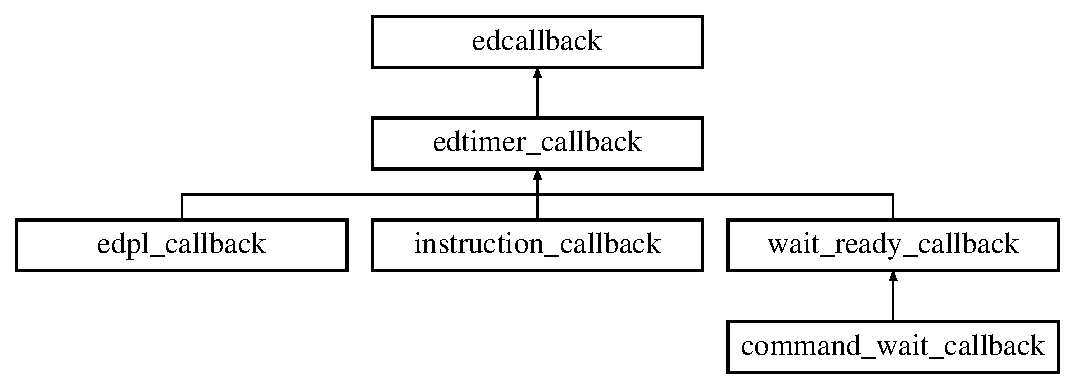
\includegraphics[height=4.000000cm]{structedtimer__callback}
\end{center}
\end{figure}
\subsection*{Public Attributes}
\begin{DoxyCompactItemize}
\item 
\hyperlink{classedtimer}{edtimer} $\ast$ \hyperlink{structedtimer__callback_a699081d4750918572f50de368e5c4536}{timer}
\end{DoxyCompactItemize}
\subsection*{Additional Inherited Members}


\subsection{Member Data Documentation}
\hypertarget{structedtimer__callback_a699081d4750918572f50de368e5c4536}{\index{edtimer\-\_\-callback@{edtimer\-\_\-callback}!timer@{timer}}
\index{timer@{timer}!edtimer_callback@{edtimer\-\_\-callback}}
\subsubsection[{timer}]{\setlength{\rightskip}{0pt plus 5cm}{\bf edtimer}$\ast$ edtimer\-\_\-callback\-::timer}}\label{structedtimer__callback_a699081d4750918572f50de368e5c4536}


The documentation for this struct was generated from the following file\-:\begin{DoxyCompactItemize}
\item 
/home/dprandle/\-Documents/code/ctrlmod/include/\hyperlink{edcallback_8h}{edcallback.\-h}\end{DoxyCompactItemize}

\hypertarget{classeduart}{\section{eduart Class Reference}
\label{classeduart}\index{eduart@{eduart}}
}


{\ttfamily \#include $<$eduart.\-h$>$}

Inheritance diagram for eduart\-:\begin{figure}[H]
\begin{center}
\leavevmode
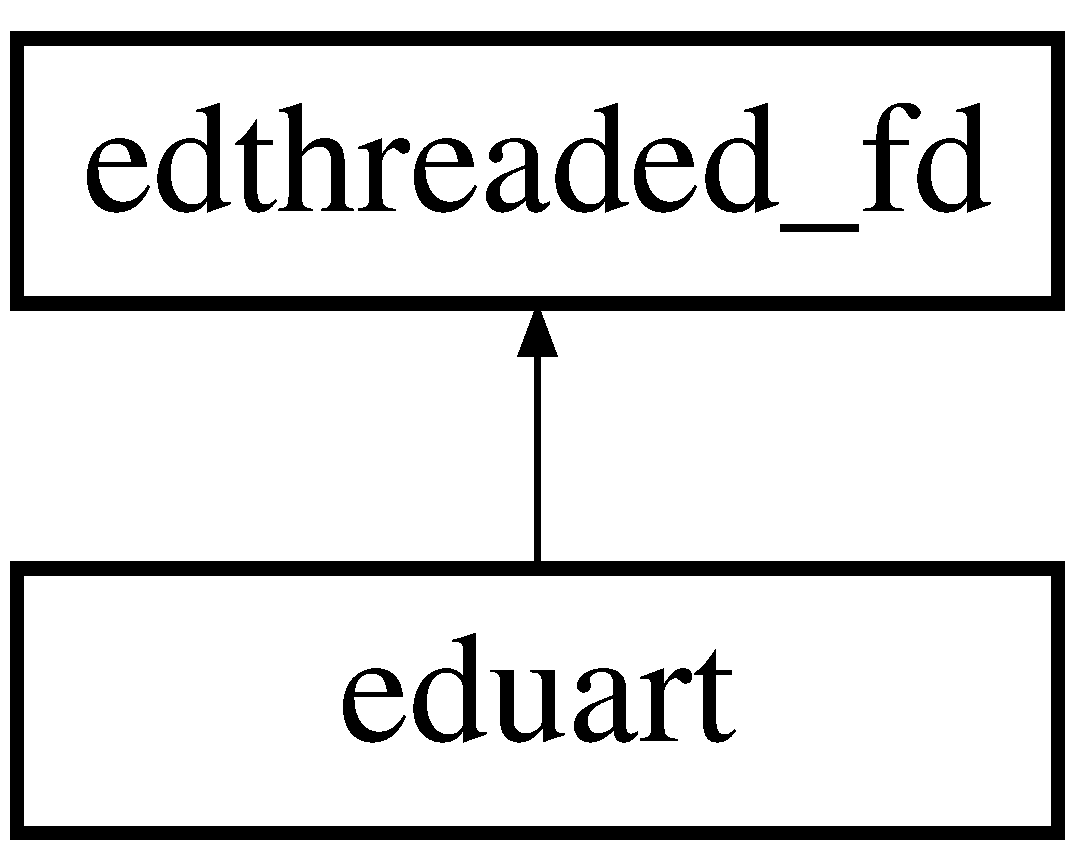
\includegraphics[height=2.000000cm]{classeduart}
\end{center}
\end{figure}
\subsection*{Classes}
\begin{DoxyCompactItemize}
\item 
struct \hyperlink{structeduart_1_1DataFormat}{Data\-Format}
\end{DoxyCompactItemize}
\subsection*{Public Types}
\begin{DoxyCompactItemize}
\item 
enum \hyperlink{classeduart_a3eb9c53aa8b561a7c0de832314e4910c}{Serial\-Port} \{ \hyperlink{classeduart_a3eb9c53aa8b561a7c0de832314e4910ca188b16da42dd309eacf50b0338c78bdc}{Uart1}, 
\hyperlink{classeduart_a3eb9c53aa8b561a7c0de832314e4910ca146f31399447a2ac2daf7c9be9e1cdb3}{Uart2}
 \}
\item 
enum \hyperlink{classeduart_af5d40999cc13e078f9d349a08ffe250e}{Baud\-Rate} \{ \\*
\hyperlink{classeduart_af5d40999cc13e078f9d349a08ffe250ea57ad9b11664ed59b685647eead7bb59a}{b50} =B50, 
\hyperlink{classeduart_af5d40999cc13e078f9d349a08ffe250ea91ba949ec01ee23fc279f2cbb1547e47}{b75} =B75, 
\hyperlink{classeduart_af5d40999cc13e078f9d349a08ffe250eac0538bdac27d5119166e538f036f51cf}{b110} =B110, 
\hyperlink{classeduart_af5d40999cc13e078f9d349a08ffe250ea40493817b15546f82e648eac9f230d55}{b134} =B134, 
\\*
\hyperlink{classeduart_af5d40999cc13e078f9d349a08ffe250eaa0d8bb58ac41d34a2921ca577c9e1dae}{b150} =B150, 
\hyperlink{classeduart_af5d40999cc13e078f9d349a08ffe250ea347b36c0426c0cfc1bba4599f0d266c5}{b200} =B200, 
\hyperlink{classeduart_af5d40999cc13e078f9d349a08ffe250ea07aed09b807d667a7edd3ada40a64f31}{b300} =B300, 
\hyperlink{classeduart_af5d40999cc13e078f9d349a08ffe250eaaaac84616144bef1e0996e666a02c082}{b600} =B600, 
\\*
\hyperlink{classeduart_af5d40999cc13e078f9d349a08ffe250eaf1d5c1b466879ebc8b27e17291736704}{b1200} =B1200, 
\hyperlink{classeduart_af5d40999cc13e078f9d349a08ffe250ea7234ba43384703cfb1457498765a21a6}{b1800} =B1800, 
\hyperlink{classeduart_af5d40999cc13e078f9d349a08ffe250ead814cc23c1ddf49585fd31d265a6ce18}{b2400} =B2400, 
\hyperlink{classeduart_af5d40999cc13e078f9d349a08ffe250ea88cd90e4c82ea7eaebec6ea8da75d166}{b4800} =B4800, 
\\*
\hyperlink{classeduart_af5d40999cc13e078f9d349a08ffe250ea428bf6af3d0fd1ba316aee1f7110ba03}{b9600} =B9600, 
\hyperlink{classeduart_af5d40999cc13e078f9d349a08ffe250ea5d53c2a6ce0485cad2ae1fba04ef4c28}{b19200} =B19200, 
\hyperlink{classeduart_af5d40999cc13e078f9d349a08ffe250eaf4a4e8cf41f6d617c882c20b7d0fcb0d}{b38400} =B38400, 
\hyperlink{classeduart_af5d40999cc13e078f9d349a08ffe250ea527aabd82f8b9089f49e03f12ee4b1bb}{b57600} =B57600, 
\\*
\hyperlink{classeduart_af5d40999cc13e078f9d349a08ffe250ea9b92eb53c2358b7349f0b0333e115712}{b115200} =B115200, 
\hyperlink{classeduart_af5d40999cc13e078f9d349a08ffe250eae8b28fbe6713439ef27be4349bf1ccc2}{b230400} =B230400, 
\hyperlink{classeduart_af5d40999cc13e078f9d349a08ffe250ea52021156eb974c70be0e2625dbed7a47}{b460800} =B460800, 
\hyperlink{classeduart_af5d40999cc13e078f9d349a08ffe250eaafe74cb93252ca06e505203cac08fb00}{b500000} =B500000, 
\\*
\hyperlink{classeduart_af5d40999cc13e078f9d349a08ffe250ea3348c0952da2487e59954c6a9c953c5a}{b576000} =B576000, 
\hyperlink{classeduart_af5d40999cc13e078f9d349a08ffe250ea7e63bfe70bb19c1ccd1e0a45f2accf18}{b921600} =B921600, 
\hyperlink{classeduart_af5d40999cc13e078f9d349a08ffe250eac5ecc01babafe93a6d81725add97ece6}{b1000000} =B1000000, 
\hyperlink{classeduart_af5d40999cc13e078f9d349a08ffe250ea774240855bae7872e7080c74766341b2}{b1152000} =B1152000, 
\\*
\hyperlink{classeduart_af5d40999cc13e078f9d349a08ffe250ea31f007d3700b2935d22fc81154bd4b8f}{b1500000} =B1500000, 
\hyperlink{classeduart_af5d40999cc13e078f9d349a08ffe250ea1062e3622afd6e2cfeee2df82430063a}{b2000000} =B2000000, 
\hyperlink{classeduart_af5d40999cc13e078f9d349a08ffe250ea4d6c5194a4986c98bc672c43f85eb234}{b2500000} =B2500000, 
\hyperlink{classeduart_af5d40999cc13e078f9d349a08ffe250ea17f9fb50ec221d64721e6d2bb85bf237}{b3000000} =B3000000, 
\\*
\hyperlink{classeduart_af5d40999cc13e078f9d349a08ffe250ead2c79beb6a3dbf5bd56b83558d1950aa}{b3500000} =B3500000, 
\hyperlink{classeduart_af5d40999cc13e078f9d349a08ffe250ea11902480c12e575e5cab69d5d9c79065}{b4000000} =B4000000
 \}
\item 
enum \hyperlink{classeduart_ab706a92a2abdd39b748492f26d89fa75}{Parity} \{ \hyperlink{classeduart_ab706a92a2abdd39b748492f26d89fa75a61946e40eb83169f78e5460d4875cb7d}{None} = 0, 
\hyperlink{classeduart_ab706a92a2abdd39b748492f26d89fa75af51fbf3ac29786606dfa6c3896c66b77}{Odd} = (P\-A\-R\-E\-N\-B $\vert$ P\-A\-R\-O\-D\-D), 
\hyperlink{classeduart_ab706a92a2abdd39b748492f26d89fa75a51c432d034dc90467584b31553a85653}{Even} = (P\-A\-R\-E\-N\-B)
 \}
\item 
enum \hyperlink{classeduart_a81d64a65349ee87e6bff9e99c1a2a4fa}{Stop\-Bits} \{ \hyperlink{classeduart_a81d64a65349ee87e6bff9e99c1a2a4faa068e1e4c3dacb4bd82e4574b3d2c04f2}{One} = 0, 
\hyperlink{classeduart_a81d64a65349ee87e6bff9e99c1a2a4faa33352b7dd8d579fb45d2bf6dd3e4f4b7}{Two} = C\-S\-T\-O\-P\-B
 \}
\item 
enum \hyperlink{classeduart_a5211d2ecc2f21296eafe114ca999abb2}{Data\-Bits} \{ \hyperlink{classeduart_a5211d2ecc2f21296eafe114ca999abb2ae5d8646efef641958f91dc4d3eaa040b}{d5} =C\-S5, 
\hyperlink{classeduart_a5211d2ecc2f21296eafe114ca999abb2aa375f36213ea175578bfea35e0b90c33}{d6} =C\-S6, 
\hyperlink{classeduart_a5211d2ecc2f21296eafe114ca999abb2a1653637ef298b2d80ec91f713c7f49f9}{d7} =C\-S7, 
\hyperlink{classeduart_a5211d2ecc2f21296eafe114ca999abb2ae277e6824ef79278ff4bebae765f2ce0}{d8} =C\-S8
 \}
\end{DoxyCompactItemize}
\subsection*{Public Member Functions}
\begin{DoxyCompactItemize}
\item 
\hyperlink{classeduart_a95a97e53a2ba1ae4bb72b39b474e8de6}{eduart} (\hyperlink{classeduart_a3eb9c53aa8b561a7c0de832314e4910c}{Serial\-Port} uart\-\_\-num)
\item 
\hyperlink{classeduart_adc0cc6a48ebaaaa297aff0c073aa8474}{$\sim$eduart} ()
\item 
const std\-::string \& \hyperlink{classeduart_ae409534073cbe8469ce8e6aed502730a}{device\-\_\-path} ()
\item 
void \hyperlink{classeduart_aef4703307a8f07bf31ec06050e5e4596}{set\-\_\-baud} (\hyperlink{classeduart_af5d40999cc13e078f9d349a08ffe250e}{Baud\-Rate} \hyperlink{classeduart_a5243e3f72554fe7463989e245e91e172}{baud})
\item 
\hyperlink{classeduart_af5d40999cc13e078f9d349a08ffe250e}{Baud\-Rate} \hyperlink{classeduart_a5243e3f72554fe7463989e245e91e172}{baud} ()
\item 
bool \hyperlink{classeduart_ae50ab2faddd54ed231380583b717ad5a}{start} ()
\item 
void \hyperlink{classeduart_ab57fd0de8fa9f541f6b925cbe53e13ba}{set\-\_\-format} (\hyperlink{classeduart_a5211d2ecc2f21296eafe114ca999abb2}{Data\-Bits} db, \hyperlink{classeduart_ab706a92a2abdd39b748492f26d89fa75}{Parity} p, \hyperlink{classeduart_a81d64a65349ee87e6bff9e99c1a2a4fa}{Stop\-Bits} sb)
\item 
void \hyperlink{classeduart_a9b5869ad89fc0c6fc14ab24485f441ed}{set\-\_\-format} (const \hyperlink{structeduart_1_1DataFormat}{Data\-Format} \&data\-\_\-format)
\item 
const \hyperlink{structeduart_1_1DataFormat}{Data\-Format} \& \hyperlink{classeduart_a5b40ea037124171636fc44f327b7bd66}{format} ()
\end{DoxyCompactItemize}
\subsection*{Additional Inherited Members}


\subsection{Member Enumeration Documentation}
\hypertarget{classeduart_af5d40999cc13e078f9d349a08ffe250e}{\index{eduart@{eduart}!Baud\-Rate@{Baud\-Rate}}
\index{Baud\-Rate@{Baud\-Rate}!eduart@{eduart}}
\subsubsection[{Baud\-Rate}]{\setlength{\rightskip}{0pt plus 5cm}enum {\bf eduart\-::\-Baud\-Rate}}}\label{classeduart_af5d40999cc13e078f9d349a08ffe250e}
\begin{Desc}
\item[Enumerator]\par
\begin{description}
\index{b50@{b50}!eduart@{eduart}}\index{eduart@{eduart}!b50@{b50}}\item[{\em 
\hypertarget{classeduart_af5d40999cc13e078f9d349a08ffe250ea57ad9b11664ed59b685647eead7bb59a}{b50}\label{classeduart_af5d40999cc13e078f9d349a08ffe250ea57ad9b11664ed59b685647eead7bb59a}
}]\index{b75@{b75}!eduart@{eduart}}\index{eduart@{eduart}!b75@{b75}}\item[{\em 
\hypertarget{classeduart_af5d40999cc13e078f9d349a08ffe250ea91ba949ec01ee23fc279f2cbb1547e47}{b75}\label{classeduart_af5d40999cc13e078f9d349a08ffe250ea91ba949ec01ee23fc279f2cbb1547e47}
}]\index{b110@{b110}!eduart@{eduart}}\index{eduart@{eduart}!b110@{b110}}\item[{\em 
\hypertarget{classeduart_af5d40999cc13e078f9d349a08ffe250eac0538bdac27d5119166e538f036f51cf}{b110}\label{classeduart_af5d40999cc13e078f9d349a08ffe250eac0538bdac27d5119166e538f036f51cf}
}]\index{b134@{b134}!eduart@{eduart}}\index{eduart@{eduart}!b134@{b134}}\item[{\em 
\hypertarget{classeduart_af5d40999cc13e078f9d349a08ffe250ea40493817b15546f82e648eac9f230d55}{b134}\label{classeduart_af5d40999cc13e078f9d349a08ffe250ea40493817b15546f82e648eac9f230d55}
}]\index{b150@{b150}!eduart@{eduart}}\index{eduart@{eduart}!b150@{b150}}\item[{\em 
\hypertarget{classeduart_af5d40999cc13e078f9d349a08ffe250eaa0d8bb58ac41d34a2921ca577c9e1dae}{b150}\label{classeduart_af5d40999cc13e078f9d349a08ffe250eaa0d8bb58ac41d34a2921ca577c9e1dae}
}]\index{b200@{b200}!eduart@{eduart}}\index{eduart@{eduart}!b200@{b200}}\item[{\em 
\hypertarget{classeduart_af5d40999cc13e078f9d349a08ffe250ea347b36c0426c0cfc1bba4599f0d266c5}{b200}\label{classeduart_af5d40999cc13e078f9d349a08ffe250ea347b36c0426c0cfc1bba4599f0d266c5}
}]\index{b300@{b300}!eduart@{eduart}}\index{eduart@{eduart}!b300@{b300}}\item[{\em 
\hypertarget{classeduart_af5d40999cc13e078f9d349a08ffe250ea07aed09b807d667a7edd3ada40a64f31}{b300}\label{classeduart_af5d40999cc13e078f9d349a08ffe250ea07aed09b807d667a7edd3ada40a64f31}
}]\index{b600@{b600}!eduart@{eduart}}\index{eduart@{eduart}!b600@{b600}}\item[{\em 
\hypertarget{classeduart_af5d40999cc13e078f9d349a08ffe250eaaaac84616144bef1e0996e666a02c082}{b600}\label{classeduart_af5d40999cc13e078f9d349a08ffe250eaaaac84616144bef1e0996e666a02c082}
}]\index{b1200@{b1200}!eduart@{eduart}}\index{eduart@{eduart}!b1200@{b1200}}\item[{\em 
\hypertarget{classeduart_af5d40999cc13e078f9d349a08ffe250eaf1d5c1b466879ebc8b27e17291736704}{b1200}\label{classeduart_af5d40999cc13e078f9d349a08ffe250eaf1d5c1b466879ebc8b27e17291736704}
}]\index{b1800@{b1800}!eduart@{eduart}}\index{eduart@{eduart}!b1800@{b1800}}\item[{\em 
\hypertarget{classeduart_af5d40999cc13e078f9d349a08ffe250ea7234ba43384703cfb1457498765a21a6}{b1800}\label{classeduart_af5d40999cc13e078f9d349a08ffe250ea7234ba43384703cfb1457498765a21a6}
}]\index{b2400@{b2400}!eduart@{eduart}}\index{eduart@{eduart}!b2400@{b2400}}\item[{\em 
\hypertarget{classeduart_af5d40999cc13e078f9d349a08ffe250ead814cc23c1ddf49585fd31d265a6ce18}{b2400}\label{classeduart_af5d40999cc13e078f9d349a08ffe250ead814cc23c1ddf49585fd31d265a6ce18}
}]\index{b4800@{b4800}!eduart@{eduart}}\index{eduart@{eduart}!b4800@{b4800}}\item[{\em 
\hypertarget{classeduart_af5d40999cc13e078f9d349a08ffe250ea88cd90e4c82ea7eaebec6ea8da75d166}{b4800}\label{classeduart_af5d40999cc13e078f9d349a08ffe250ea88cd90e4c82ea7eaebec6ea8da75d166}
}]\index{b9600@{b9600}!eduart@{eduart}}\index{eduart@{eduart}!b9600@{b9600}}\item[{\em 
\hypertarget{classeduart_af5d40999cc13e078f9d349a08ffe250ea428bf6af3d0fd1ba316aee1f7110ba03}{b9600}\label{classeduart_af5d40999cc13e078f9d349a08ffe250ea428bf6af3d0fd1ba316aee1f7110ba03}
}]\index{b19200@{b19200}!eduart@{eduart}}\index{eduart@{eduart}!b19200@{b19200}}\item[{\em 
\hypertarget{classeduart_af5d40999cc13e078f9d349a08ffe250ea5d53c2a6ce0485cad2ae1fba04ef4c28}{b19200}\label{classeduart_af5d40999cc13e078f9d349a08ffe250ea5d53c2a6ce0485cad2ae1fba04ef4c28}
}]\index{b38400@{b38400}!eduart@{eduart}}\index{eduart@{eduart}!b38400@{b38400}}\item[{\em 
\hypertarget{classeduart_af5d40999cc13e078f9d349a08ffe250eaf4a4e8cf41f6d617c882c20b7d0fcb0d}{b38400}\label{classeduart_af5d40999cc13e078f9d349a08ffe250eaf4a4e8cf41f6d617c882c20b7d0fcb0d}
}]\index{b57600@{b57600}!eduart@{eduart}}\index{eduart@{eduart}!b57600@{b57600}}\item[{\em 
\hypertarget{classeduart_af5d40999cc13e078f9d349a08ffe250ea527aabd82f8b9089f49e03f12ee4b1bb}{b57600}\label{classeduart_af5d40999cc13e078f9d349a08ffe250ea527aabd82f8b9089f49e03f12ee4b1bb}
}]\index{b115200@{b115200}!eduart@{eduart}}\index{eduart@{eduart}!b115200@{b115200}}\item[{\em 
\hypertarget{classeduart_af5d40999cc13e078f9d349a08ffe250ea9b92eb53c2358b7349f0b0333e115712}{b115200}\label{classeduart_af5d40999cc13e078f9d349a08ffe250ea9b92eb53c2358b7349f0b0333e115712}
}]\index{b230400@{b230400}!eduart@{eduart}}\index{eduart@{eduart}!b230400@{b230400}}\item[{\em 
\hypertarget{classeduart_af5d40999cc13e078f9d349a08ffe250eae8b28fbe6713439ef27be4349bf1ccc2}{b230400}\label{classeduart_af5d40999cc13e078f9d349a08ffe250eae8b28fbe6713439ef27be4349bf1ccc2}
}]\index{b460800@{b460800}!eduart@{eduart}}\index{eduart@{eduart}!b460800@{b460800}}\item[{\em 
\hypertarget{classeduart_af5d40999cc13e078f9d349a08ffe250ea52021156eb974c70be0e2625dbed7a47}{b460800}\label{classeduart_af5d40999cc13e078f9d349a08ffe250ea52021156eb974c70be0e2625dbed7a47}
}]\index{b500000@{b500000}!eduart@{eduart}}\index{eduart@{eduart}!b500000@{b500000}}\item[{\em 
\hypertarget{classeduart_af5d40999cc13e078f9d349a08ffe250eaafe74cb93252ca06e505203cac08fb00}{b500000}\label{classeduart_af5d40999cc13e078f9d349a08ffe250eaafe74cb93252ca06e505203cac08fb00}
}]\index{b576000@{b576000}!eduart@{eduart}}\index{eduart@{eduart}!b576000@{b576000}}\item[{\em 
\hypertarget{classeduart_af5d40999cc13e078f9d349a08ffe250ea3348c0952da2487e59954c6a9c953c5a}{b576000}\label{classeduart_af5d40999cc13e078f9d349a08ffe250ea3348c0952da2487e59954c6a9c953c5a}
}]\index{b921600@{b921600}!eduart@{eduart}}\index{eduart@{eduart}!b921600@{b921600}}\item[{\em 
\hypertarget{classeduart_af5d40999cc13e078f9d349a08ffe250ea7e63bfe70bb19c1ccd1e0a45f2accf18}{b921600}\label{classeduart_af5d40999cc13e078f9d349a08ffe250ea7e63bfe70bb19c1ccd1e0a45f2accf18}
}]\index{b1000000@{b1000000}!eduart@{eduart}}\index{eduart@{eduart}!b1000000@{b1000000}}\item[{\em 
\hypertarget{classeduart_af5d40999cc13e078f9d349a08ffe250eac5ecc01babafe93a6d81725add97ece6}{b1000000}\label{classeduart_af5d40999cc13e078f9d349a08ffe250eac5ecc01babafe93a6d81725add97ece6}
}]\index{b1152000@{b1152000}!eduart@{eduart}}\index{eduart@{eduart}!b1152000@{b1152000}}\item[{\em 
\hypertarget{classeduart_af5d40999cc13e078f9d349a08ffe250ea774240855bae7872e7080c74766341b2}{b1152000}\label{classeduart_af5d40999cc13e078f9d349a08ffe250ea774240855bae7872e7080c74766341b2}
}]\index{b1500000@{b1500000}!eduart@{eduart}}\index{eduart@{eduart}!b1500000@{b1500000}}\item[{\em 
\hypertarget{classeduart_af5d40999cc13e078f9d349a08ffe250ea31f007d3700b2935d22fc81154bd4b8f}{b1500000}\label{classeduart_af5d40999cc13e078f9d349a08ffe250ea31f007d3700b2935d22fc81154bd4b8f}
}]\index{b2000000@{b2000000}!eduart@{eduart}}\index{eduart@{eduart}!b2000000@{b2000000}}\item[{\em 
\hypertarget{classeduart_af5d40999cc13e078f9d349a08ffe250ea1062e3622afd6e2cfeee2df82430063a}{b2000000}\label{classeduart_af5d40999cc13e078f9d349a08ffe250ea1062e3622afd6e2cfeee2df82430063a}
}]\index{b2500000@{b2500000}!eduart@{eduart}}\index{eduart@{eduart}!b2500000@{b2500000}}\item[{\em 
\hypertarget{classeduart_af5d40999cc13e078f9d349a08ffe250ea4d6c5194a4986c98bc672c43f85eb234}{b2500000}\label{classeduart_af5d40999cc13e078f9d349a08ffe250ea4d6c5194a4986c98bc672c43f85eb234}
}]\index{b3000000@{b3000000}!eduart@{eduart}}\index{eduart@{eduart}!b3000000@{b3000000}}\item[{\em 
\hypertarget{classeduart_af5d40999cc13e078f9d349a08ffe250ea17f9fb50ec221d64721e6d2bb85bf237}{b3000000}\label{classeduart_af5d40999cc13e078f9d349a08ffe250ea17f9fb50ec221d64721e6d2bb85bf237}
}]\index{b3500000@{b3500000}!eduart@{eduart}}\index{eduart@{eduart}!b3500000@{b3500000}}\item[{\em 
\hypertarget{classeduart_af5d40999cc13e078f9d349a08ffe250ead2c79beb6a3dbf5bd56b83558d1950aa}{b3500000}\label{classeduart_af5d40999cc13e078f9d349a08ffe250ead2c79beb6a3dbf5bd56b83558d1950aa}
}]\index{b4000000@{b4000000}!eduart@{eduart}}\index{eduart@{eduart}!b4000000@{b4000000}}\item[{\em 
\hypertarget{classeduart_af5d40999cc13e078f9d349a08ffe250ea11902480c12e575e5cab69d5d9c79065}{b4000000}\label{classeduart_af5d40999cc13e078f9d349a08ffe250ea11902480c12e575e5cab69d5d9c79065}
}]\end{description}
\end{Desc}
\hypertarget{classeduart_a5211d2ecc2f21296eafe114ca999abb2}{\index{eduart@{eduart}!Data\-Bits@{Data\-Bits}}
\index{Data\-Bits@{Data\-Bits}!eduart@{eduart}}
\subsubsection[{Data\-Bits}]{\setlength{\rightskip}{0pt plus 5cm}enum {\bf eduart\-::\-Data\-Bits}}}\label{classeduart_a5211d2ecc2f21296eafe114ca999abb2}
\begin{Desc}
\item[Enumerator]\par
\begin{description}
\index{d5@{d5}!eduart@{eduart}}\index{eduart@{eduart}!d5@{d5}}\item[{\em 
\hypertarget{classeduart_a5211d2ecc2f21296eafe114ca999abb2ae5d8646efef641958f91dc4d3eaa040b}{d5}\label{classeduart_a5211d2ecc2f21296eafe114ca999abb2ae5d8646efef641958f91dc4d3eaa040b}
}]\index{d6@{d6}!eduart@{eduart}}\index{eduart@{eduart}!d6@{d6}}\item[{\em 
\hypertarget{classeduart_a5211d2ecc2f21296eafe114ca999abb2aa375f36213ea175578bfea35e0b90c33}{d6}\label{classeduart_a5211d2ecc2f21296eafe114ca999abb2aa375f36213ea175578bfea35e0b90c33}
}]\index{d7@{d7}!eduart@{eduart}}\index{eduart@{eduart}!d7@{d7}}\item[{\em 
\hypertarget{classeduart_a5211d2ecc2f21296eafe114ca999abb2a1653637ef298b2d80ec91f713c7f49f9}{d7}\label{classeduart_a5211d2ecc2f21296eafe114ca999abb2a1653637ef298b2d80ec91f713c7f49f9}
}]\index{d8@{d8}!eduart@{eduart}}\index{eduart@{eduart}!d8@{d8}}\item[{\em 
\hypertarget{classeduart_a5211d2ecc2f21296eafe114ca999abb2ae277e6824ef79278ff4bebae765f2ce0}{d8}\label{classeduart_a5211d2ecc2f21296eafe114ca999abb2ae277e6824ef79278ff4bebae765f2ce0}
}]\end{description}
\end{Desc}
\hypertarget{classeduart_ab706a92a2abdd39b748492f26d89fa75}{\index{eduart@{eduart}!Parity@{Parity}}
\index{Parity@{Parity}!eduart@{eduart}}
\subsubsection[{Parity}]{\setlength{\rightskip}{0pt plus 5cm}enum {\bf eduart\-::\-Parity}}}\label{classeduart_ab706a92a2abdd39b748492f26d89fa75}
\begin{Desc}
\item[Enumerator]\par
\begin{description}
\index{None@{None}!eduart@{eduart}}\index{eduart@{eduart}!None@{None}}\item[{\em 
\hypertarget{classeduart_ab706a92a2abdd39b748492f26d89fa75a61946e40eb83169f78e5460d4875cb7d}{None}\label{classeduart_ab706a92a2abdd39b748492f26d89fa75a61946e40eb83169f78e5460d4875cb7d}
}]\index{Odd@{Odd}!eduart@{eduart}}\index{eduart@{eduart}!Odd@{Odd}}\item[{\em 
\hypertarget{classeduart_ab706a92a2abdd39b748492f26d89fa75af51fbf3ac29786606dfa6c3896c66b77}{Odd}\label{classeduart_ab706a92a2abdd39b748492f26d89fa75af51fbf3ac29786606dfa6c3896c66b77}
}]\index{Even@{Even}!eduart@{eduart}}\index{eduart@{eduart}!Even@{Even}}\item[{\em 
\hypertarget{classeduart_ab706a92a2abdd39b748492f26d89fa75a51c432d034dc90467584b31553a85653}{Even}\label{classeduart_ab706a92a2abdd39b748492f26d89fa75a51c432d034dc90467584b31553a85653}
}]\end{description}
\end{Desc}
\hypertarget{classeduart_a3eb9c53aa8b561a7c0de832314e4910c}{\index{eduart@{eduart}!Serial\-Port@{Serial\-Port}}
\index{Serial\-Port@{Serial\-Port}!eduart@{eduart}}
\subsubsection[{Serial\-Port}]{\setlength{\rightskip}{0pt plus 5cm}enum {\bf eduart\-::\-Serial\-Port}}}\label{classeduart_a3eb9c53aa8b561a7c0de832314e4910c}
\begin{Desc}
\item[Enumerator]\par
\begin{description}
\index{Uart1@{Uart1}!eduart@{eduart}}\index{eduart@{eduart}!Uart1@{Uart1}}\item[{\em 
\hypertarget{classeduart_a3eb9c53aa8b561a7c0de832314e4910ca188b16da42dd309eacf50b0338c78bdc}{Uart1}\label{classeduart_a3eb9c53aa8b561a7c0de832314e4910ca188b16da42dd309eacf50b0338c78bdc}
}]\index{Uart2@{Uart2}!eduart@{eduart}}\index{eduart@{eduart}!Uart2@{Uart2}}\item[{\em 
\hypertarget{classeduart_a3eb9c53aa8b561a7c0de832314e4910ca146f31399447a2ac2daf7c9be9e1cdb3}{Uart2}\label{classeduart_a3eb9c53aa8b561a7c0de832314e4910ca146f31399447a2ac2daf7c9be9e1cdb3}
}]\end{description}
\end{Desc}
\hypertarget{classeduart_a81d64a65349ee87e6bff9e99c1a2a4fa}{\index{eduart@{eduart}!Stop\-Bits@{Stop\-Bits}}
\index{Stop\-Bits@{Stop\-Bits}!eduart@{eduart}}
\subsubsection[{Stop\-Bits}]{\setlength{\rightskip}{0pt plus 5cm}enum {\bf eduart\-::\-Stop\-Bits}}}\label{classeduart_a81d64a65349ee87e6bff9e99c1a2a4fa}
\begin{Desc}
\item[Enumerator]\par
\begin{description}
\index{One@{One}!eduart@{eduart}}\index{eduart@{eduart}!One@{One}}\item[{\em 
\hypertarget{classeduart_a81d64a65349ee87e6bff9e99c1a2a4faa068e1e4c3dacb4bd82e4574b3d2c04f2}{One}\label{classeduart_a81d64a65349ee87e6bff9e99c1a2a4faa068e1e4c3dacb4bd82e4574b3d2c04f2}
}]\index{Two@{Two}!eduart@{eduart}}\index{eduart@{eduart}!Two@{Two}}\item[{\em 
\hypertarget{classeduart_a81d64a65349ee87e6bff9e99c1a2a4faa33352b7dd8d579fb45d2bf6dd3e4f4b7}{Two}\label{classeduart_a81d64a65349ee87e6bff9e99c1a2a4faa33352b7dd8d579fb45d2bf6dd3e4f4b7}
}]\end{description}
\end{Desc}


\subsection{Constructor \& Destructor Documentation}
\hypertarget{classeduart_a95a97e53a2ba1ae4bb72b39b474e8de6}{\index{eduart@{eduart}!eduart@{eduart}}
\index{eduart@{eduart}!eduart@{eduart}}
\subsubsection[{eduart}]{\setlength{\rightskip}{0pt plus 5cm}eduart\-::eduart (
\begin{DoxyParamCaption}
\item[{{\bf Serial\-Port}}]{uart\-\_\-num}
\end{DoxyParamCaption}
)}}\label{classeduart_a95a97e53a2ba1ae4bb72b39b474e8de6}
\hypertarget{classeduart_adc0cc6a48ebaaaa297aff0c073aa8474}{\index{eduart@{eduart}!$\sim$eduart@{$\sim$eduart}}
\index{$\sim$eduart@{$\sim$eduart}!eduart@{eduart}}
\subsubsection[{$\sim$eduart}]{\setlength{\rightskip}{0pt plus 5cm}eduart\-::$\sim$eduart (
\begin{DoxyParamCaption}
{}
\end{DoxyParamCaption}
)}}\label{classeduart_adc0cc6a48ebaaaa297aff0c073aa8474}


\subsection{Member Function Documentation}
\hypertarget{classeduart_a5243e3f72554fe7463989e245e91e172}{\index{eduart@{eduart}!baud@{baud}}
\index{baud@{baud}!eduart@{eduart}}
\subsubsection[{baud}]{\setlength{\rightskip}{0pt plus 5cm}{\bf eduart\-::\-Baud\-Rate} eduart\-::baud (
\begin{DoxyParamCaption}
{}
\end{DoxyParamCaption}
)}}\label{classeduart_a5243e3f72554fe7463989e245e91e172}
\hypertarget{classeduart_ae409534073cbe8469ce8e6aed502730a}{\index{eduart@{eduart}!device\-\_\-path@{device\-\_\-path}}
\index{device\-\_\-path@{device\-\_\-path}!eduart@{eduart}}
\subsubsection[{device\-\_\-path}]{\setlength{\rightskip}{0pt plus 5cm}const std\-::string \& eduart\-::device\-\_\-path (
\begin{DoxyParamCaption}
{}
\end{DoxyParamCaption}
)}}\label{classeduart_ae409534073cbe8469ce8e6aed502730a}
\hypertarget{classeduart_a5b40ea037124171636fc44f327b7bd66}{\index{eduart@{eduart}!format@{format}}
\index{format@{format}!eduart@{eduart}}
\subsubsection[{format}]{\setlength{\rightskip}{0pt plus 5cm}const {\bf eduart\-::\-Data\-Format} \& eduart\-::format (
\begin{DoxyParamCaption}
{}
\end{DoxyParamCaption}
)}}\label{classeduart_a5b40ea037124171636fc44f327b7bd66}
\hypertarget{classeduart_aef4703307a8f07bf31ec06050e5e4596}{\index{eduart@{eduart}!set\-\_\-baud@{set\-\_\-baud}}
\index{set\-\_\-baud@{set\-\_\-baud}!eduart@{eduart}}
\subsubsection[{set\-\_\-baud}]{\setlength{\rightskip}{0pt plus 5cm}void eduart\-::set\-\_\-baud (
\begin{DoxyParamCaption}
\item[{{\bf Baud\-Rate}}]{baud}
\end{DoxyParamCaption}
)}}\label{classeduart_aef4703307a8f07bf31ec06050e5e4596}
\hypertarget{classeduart_ab57fd0de8fa9f541f6b925cbe53e13ba}{\index{eduart@{eduart}!set\-\_\-format@{set\-\_\-format}}
\index{set\-\_\-format@{set\-\_\-format}!eduart@{eduart}}
\subsubsection[{set\-\_\-format}]{\setlength{\rightskip}{0pt plus 5cm}void eduart\-::set\-\_\-format (
\begin{DoxyParamCaption}
\item[{{\bf Data\-Bits}}]{db, }
\item[{{\bf Parity}}]{p, }
\item[{{\bf Stop\-Bits}}]{sb}
\end{DoxyParamCaption}
)}}\label{classeduart_ab57fd0de8fa9f541f6b925cbe53e13ba}
\hypertarget{classeduart_a9b5869ad89fc0c6fc14ab24485f441ed}{\index{eduart@{eduart}!set\-\_\-format@{set\-\_\-format}}
\index{set\-\_\-format@{set\-\_\-format}!eduart@{eduart}}
\subsubsection[{set\-\_\-format}]{\setlength{\rightskip}{0pt plus 5cm}void eduart\-::set\-\_\-format (
\begin{DoxyParamCaption}
\item[{const {\bf Data\-Format} \&}]{data\-\_\-format}
\end{DoxyParamCaption}
)}}\label{classeduart_a9b5869ad89fc0c6fc14ab24485f441ed}
\hypertarget{classeduart_ae50ab2faddd54ed231380583b717ad5a}{\index{eduart@{eduart}!start@{start}}
\index{start@{start}!eduart@{eduart}}
\subsubsection[{start}]{\setlength{\rightskip}{0pt plus 5cm}bool eduart\-::start (
\begin{DoxyParamCaption}
{}
\end{DoxyParamCaption}
)\hspace{0.3cm}{\ttfamily [virtual]}}}\label{classeduart_ae50ab2faddd54ed231380583b717ad5a}


Reimplemented from \hyperlink{classedthreaded__fd_ac8123803d831c671b9b62881697e69e0}{edthreaded\-\_\-fd}.



The documentation for this class was generated from the following files\-:\begin{DoxyCompactItemize}
\item 
/home/dprandle/\-Documents/code/ctrlmod/include/\hyperlink{eduart_8h}{eduart.\-h}\item 
/home/dprandle/\-Documents/code/ctrlmod/src/\hyperlink{eduart_8cpp}{eduart.\-cpp}\end{DoxyCompactItemize}

\hypertarget{structedthreaded__fd_1_1Error}{\section{edthreaded\-\_\-fd\-:\-:Error Struct Reference}
\label{structedthreaded__fd_1_1Error}\index{edthreaded\-\_\-fd\-::\-Error@{edthreaded\-\_\-fd\-::\-Error}}
}


{\ttfamily \#include $<$edthreaded\-\_\-fd.\-h$>$}

\subsection*{Public Member Functions}
\begin{DoxyCompactItemize}
\item 
\hyperlink{structedthreaded__fd_1_1Error_ae5715fd2bb0bf1a86a13d6bfa17cf6bf}{Error} ()
\end{DoxyCompactItemize}
\subsection*{Public Attributes}
\begin{DoxyCompactItemize}
\item 
\hyperlink{classedthreaded__fd_ab3562872429271887a15489b7a1a17d7}{Error\-Val} \hyperlink{structedthreaded__fd_1_1Error_acc3972f4951454b71a97e3ede3dccb40}{err\-\_\-val}
\item 
int32\-\_\-t \hyperlink{structedthreaded__fd_1_1Error_a41ad28fb17556cff7060fc6eb7bbab75}{\-\_\-errno}
\end{DoxyCompactItemize}


\subsection{Constructor \& Destructor Documentation}
\hypertarget{structedthreaded__fd_1_1Error_ae5715fd2bb0bf1a86a13d6bfa17cf6bf}{\index{edthreaded\-\_\-fd\-::\-Error@{edthreaded\-\_\-fd\-::\-Error}!Error@{Error}}
\index{Error@{Error}!edthreaded_fd::Error@{edthreaded\-\_\-fd\-::\-Error}}
\subsubsection[{Error}]{\setlength{\rightskip}{0pt plus 5cm}edthreaded\-\_\-fd\-::\-Error\-::\-Error (
\begin{DoxyParamCaption}
{}
\end{DoxyParamCaption}
)\hspace{0.3cm}{\ttfamily [inline]}}}\label{structedthreaded__fd_1_1Error_ae5715fd2bb0bf1a86a13d6bfa17cf6bf}


\subsection{Member Data Documentation}
\hypertarget{structedthreaded__fd_1_1Error_a41ad28fb17556cff7060fc6eb7bbab75}{\index{edthreaded\-\_\-fd\-::\-Error@{edthreaded\-\_\-fd\-::\-Error}!\-\_\-errno@{\-\_\-errno}}
\index{\-\_\-errno@{\-\_\-errno}!edthreaded_fd::Error@{edthreaded\-\_\-fd\-::\-Error}}
\subsubsection[{\-\_\-errno}]{\setlength{\rightskip}{0pt plus 5cm}int32\-\_\-t edthreaded\-\_\-fd\-::\-Error\-::\-\_\-errno}}\label{structedthreaded__fd_1_1Error_a41ad28fb17556cff7060fc6eb7bbab75}
\hypertarget{structedthreaded__fd_1_1Error_acc3972f4951454b71a97e3ede3dccb40}{\index{edthreaded\-\_\-fd\-::\-Error@{edthreaded\-\_\-fd\-::\-Error}!err\-\_\-val@{err\-\_\-val}}
\index{err\-\_\-val@{err\-\_\-val}!edthreaded_fd::Error@{edthreaded\-\_\-fd\-::\-Error}}
\subsubsection[{err\-\_\-val}]{\setlength{\rightskip}{0pt plus 5cm}{\bf Error\-Val} edthreaded\-\_\-fd\-::\-Error\-::err\-\_\-val}}\label{structedthreaded__fd_1_1Error_acc3972f4951454b71a97e3ede3dccb40}


The documentation for this struct was generated from the following file\-:\begin{DoxyCompactItemize}
\item 
/home/dprandle/\-Documents/code/ctrlmod/include/\hyperlink{edthreaded__fd_8h}{edthreaded\-\_\-fd.\-h}\end{DoxyCompactItemize}

\hypertarget{structfirmware__data__packet}{\section{firmware\-\_\-data\-\_\-packet Struct Reference}
\label{structfirmware__data__packet}\index{firmware\-\_\-data\-\_\-packet@{firmware\-\_\-data\-\_\-packet}}
}


{\ttfamily \#include $<$edrplidar\-\_\-packets.\-h$>$}

Inheritance diagram for firmware\-\_\-data\-\_\-packet\-:\begin{figure}[H]
\begin{center}
\leavevmode
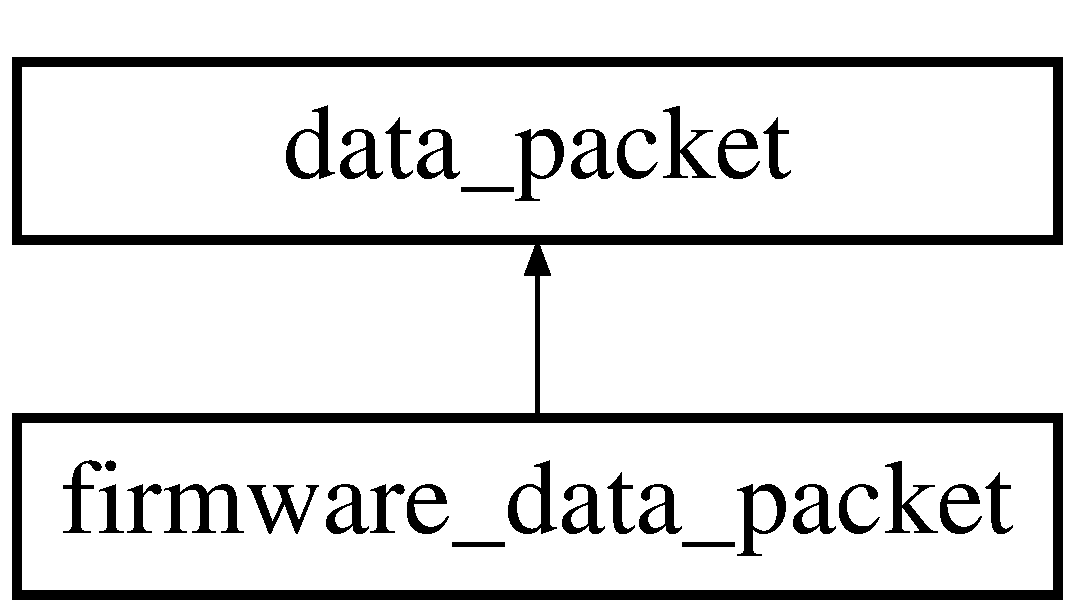
\includegraphics[height=2.000000cm]{structfirmware__data__packet}
\end{center}
\end{figure}
\subsection*{Public Member Functions}
\begin{DoxyCompactItemize}
\item 
\hyperlink{structfirmware__data__packet_a084123acea6482ea08949203f5ed9f40}{firmware\-\_\-data\-\_\-packet} ()
\item 
virtual std\-::string \hyperlink{structfirmware__data__packet_a1ff72c5345b4325fd955bb20c9860d89}{to\-String} ()
\item 
virtual std\-::string \hyperlink{structfirmware__data__packet_a84cd6f60b9d5ef46ab5c4695d6de3d48}{type} ()
\item 
virtual uint32\-\_\-t \hyperlink{structfirmware__data__packet_a3231148228aee555265b90ab30fea9ec}{size} ()
\item 
virtual uint8\-\_\-t \& \hyperlink{structfirmware__data__packet_a16d28be180847cb45fc4dbf0417756b9}{operator\mbox{[}$\,$\mbox{]}} (uint32\-\_\-t index)
\item 
virtual uint8\-\_\-t $\ast$ \hyperlink{structfirmware__data__packet_ab080f05c847592a2578ee307d5af31fc}{dataptr} ()
\end{DoxyCompactItemize}
\subsection*{Static Public Member Functions}
\begin{DoxyCompactItemize}
\item 
static std\-::string \hyperlink{structfirmware__data__packet_a6b386640d9fa172bfa44c55d63add943}{Type} ()
\item 
static uint32\-\_\-t \hyperlink{structfirmware__data__packet_a91ec8c2d5f0f7f642027b0ed566417d0}{Size} ()
\end{DoxyCompactItemize}
\subsection*{Public Attributes}
\begin{DoxyCompactItemize}
\item 
\begin{tabbing}
xx\=xx\=xx\=xx\=xx\=xx\=xx\=xx\=xx\=\kill
union \{\\
\>struct \{\\
\>\>uint8\_t \hyperlink{structfirmware__data__packet_a47aec40c2fc17de6c7a60eba35776e7d}{line1} \mbox{[}18\mbox{]}\\
\>\>uint8\_t \hyperlink{structfirmware__data__packet_ac9cd94ddddd471656eb5ec03914ffc1c}{line2} \mbox{[}29\mbox{]}\\
\>\>uint8\_t \hyperlink{structfirmware__data__packet_a943cd8ef900bcfffba560cd718c2f844}{line3} \mbox{[}9\mbox{]}\\
\>\} \\
\>uint8\_t \hyperlink{structfirmware__data__packet_a224c1a6c9d1cf15546679bd74d793f2e}{data} \mbox{[}56\mbox{]}\\
\}; \\

\end{tabbing}\end{DoxyCompactItemize}


\subsection{Constructor \& Destructor Documentation}
\hypertarget{structfirmware__data__packet_a084123acea6482ea08949203f5ed9f40}{\index{firmware\-\_\-data\-\_\-packet@{firmware\-\_\-data\-\_\-packet}!firmware\-\_\-data\-\_\-packet@{firmware\-\_\-data\-\_\-packet}}
\index{firmware\-\_\-data\-\_\-packet@{firmware\-\_\-data\-\_\-packet}!firmware_data_packet@{firmware\-\_\-data\-\_\-packet}}
\subsubsection[{firmware\-\_\-data\-\_\-packet}]{\setlength{\rightskip}{0pt plus 5cm}firmware\-\_\-data\-\_\-packet\-::firmware\-\_\-data\-\_\-packet (
\begin{DoxyParamCaption}
{}
\end{DoxyParamCaption}
)}}\label{structfirmware__data__packet_a084123acea6482ea08949203f5ed9f40}


\subsection{Member Function Documentation}
\hypertarget{structfirmware__data__packet_ab080f05c847592a2578ee307d5af31fc}{\index{firmware\-\_\-data\-\_\-packet@{firmware\-\_\-data\-\_\-packet}!dataptr@{dataptr}}
\index{dataptr@{dataptr}!firmware_data_packet@{firmware\-\_\-data\-\_\-packet}}
\subsubsection[{dataptr}]{\setlength{\rightskip}{0pt plus 5cm}virtual uint8\-\_\-t$\ast$ firmware\-\_\-data\-\_\-packet\-::dataptr (
\begin{DoxyParamCaption}
{}
\end{DoxyParamCaption}
)\hspace{0.3cm}{\ttfamily [inline]}, {\ttfamily [virtual]}}}\label{structfirmware__data__packet_ab080f05c847592a2578ee307d5af31fc}


Implements \hyperlink{structdata__packet_ac53dcca572fc7cf7d71ae21d5c785365}{data\-\_\-packet}.

\hypertarget{structfirmware__data__packet_a16d28be180847cb45fc4dbf0417756b9}{\index{firmware\-\_\-data\-\_\-packet@{firmware\-\_\-data\-\_\-packet}!operator\mbox{[}$\,$\mbox{]}@{operator[]}}
\index{operator\mbox{[}$\,$\mbox{]}@{operator[]}!firmware_data_packet@{firmware\-\_\-data\-\_\-packet}}
\subsubsection[{operator[]}]{\setlength{\rightskip}{0pt plus 5cm}virtual uint8\-\_\-t\& firmware\-\_\-data\-\_\-packet\-::operator\mbox{[}$\,$\mbox{]} (
\begin{DoxyParamCaption}
\item[{uint32\-\_\-t}]{index}
\end{DoxyParamCaption}
)\hspace{0.3cm}{\ttfamily [inline]}, {\ttfamily [virtual]}}}\label{structfirmware__data__packet_a16d28be180847cb45fc4dbf0417756b9}


Implements \hyperlink{structdata__packet_a8f0d95d4a7a7089b45cef14e45b0c21b}{data\-\_\-packet}.

\hypertarget{structfirmware__data__packet_a3231148228aee555265b90ab30fea9ec}{\index{firmware\-\_\-data\-\_\-packet@{firmware\-\_\-data\-\_\-packet}!size@{size}}
\index{size@{size}!firmware_data_packet@{firmware\-\_\-data\-\_\-packet}}
\subsubsection[{size}]{\setlength{\rightskip}{0pt plus 5cm}virtual uint32\-\_\-t firmware\-\_\-data\-\_\-packet\-::size (
\begin{DoxyParamCaption}
{}
\end{DoxyParamCaption}
)\hspace{0.3cm}{\ttfamily [inline]}, {\ttfamily [virtual]}}}\label{structfirmware__data__packet_a3231148228aee555265b90ab30fea9ec}


Implements \hyperlink{structdata__packet_ab5c9259a79cde0dc60d75135fe8464f6}{data\-\_\-packet}.

\hypertarget{structfirmware__data__packet_a91ec8c2d5f0f7f642027b0ed566417d0}{\index{firmware\-\_\-data\-\_\-packet@{firmware\-\_\-data\-\_\-packet}!Size@{Size}}
\index{Size@{Size}!firmware_data_packet@{firmware\-\_\-data\-\_\-packet}}
\subsubsection[{Size}]{\setlength{\rightskip}{0pt plus 5cm}static uint32\-\_\-t firmware\-\_\-data\-\_\-packet\-::\-Size (
\begin{DoxyParamCaption}
{}
\end{DoxyParamCaption}
)\hspace{0.3cm}{\ttfamily [inline]}, {\ttfamily [static]}}}\label{structfirmware__data__packet_a91ec8c2d5f0f7f642027b0ed566417d0}
\hypertarget{structfirmware__data__packet_a1ff72c5345b4325fd955bb20c9860d89}{\index{firmware\-\_\-data\-\_\-packet@{firmware\-\_\-data\-\_\-packet}!to\-String@{to\-String}}
\index{to\-String@{to\-String}!firmware_data_packet@{firmware\-\_\-data\-\_\-packet}}
\subsubsection[{to\-String}]{\setlength{\rightskip}{0pt plus 5cm}std\-::string firmware\-\_\-data\-\_\-packet\-::to\-String (
\begin{DoxyParamCaption}
{}
\end{DoxyParamCaption}
)\hspace{0.3cm}{\ttfamily [virtual]}}}\label{structfirmware__data__packet_a1ff72c5345b4325fd955bb20c9860d89}


Implements \hyperlink{structdata__packet_ad7ce179caef76c895bfc778862bc15ac}{data\-\_\-packet}.

\hypertarget{structfirmware__data__packet_a84cd6f60b9d5ef46ab5c4695d6de3d48}{\index{firmware\-\_\-data\-\_\-packet@{firmware\-\_\-data\-\_\-packet}!type@{type}}
\index{type@{type}!firmware_data_packet@{firmware\-\_\-data\-\_\-packet}}
\subsubsection[{type}]{\setlength{\rightskip}{0pt plus 5cm}virtual std\-::string firmware\-\_\-data\-\_\-packet\-::type (
\begin{DoxyParamCaption}
{}
\end{DoxyParamCaption}
)\hspace{0.3cm}{\ttfamily [inline]}, {\ttfamily [virtual]}}}\label{structfirmware__data__packet_a84cd6f60b9d5ef46ab5c4695d6de3d48}


Implements \hyperlink{structdata__packet_af0795581f2d57a8c14a88009da37aee1}{data\-\_\-packet}.

\hypertarget{structfirmware__data__packet_a6b386640d9fa172bfa44c55d63add943}{\index{firmware\-\_\-data\-\_\-packet@{firmware\-\_\-data\-\_\-packet}!Type@{Type}}
\index{Type@{Type}!firmware_data_packet@{firmware\-\_\-data\-\_\-packet}}
\subsubsection[{Type}]{\setlength{\rightskip}{0pt plus 5cm}static std\-::string firmware\-\_\-data\-\_\-packet\-::\-Type (
\begin{DoxyParamCaption}
{}
\end{DoxyParamCaption}
)\hspace{0.3cm}{\ttfamily [inline]}, {\ttfamily [static]}}}\label{structfirmware__data__packet_a6b386640d9fa172bfa44c55d63add943}


\subsection{Member Data Documentation}
\hypertarget{structfirmware__data__packet_a251e81785646ac043c47035095aaea9d}{\subsubsection[{"@25}]{\setlength{\rightskip}{0pt plus 5cm}union \{ ... \} }}\label{structfirmware__data__packet_a251e81785646ac043c47035095aaea9d}
\hypertarget{structfirmware__data__packet_a224c1a6c9d1cf15546679bd74d793f2e}{\index{firmware\-\_\-data\-\_\-packet@{firmware\-\_\-data\-\_\-packet}!data@{data}}
\index{data@{data}!firmware_data_packet@{firmware\-\_\-data\-\_\-packet}}
\subsubsection[{data}]{\setlength{\rightskip}{0pt plus 5cm}uint8\-\_\-t firmware\-\_\-data\-\_\-packet\-::data\mbox{[}56\mbox{]}}}\label{structfirmware__data__packet_a224c1a6c9d1cf15546679bd74d793f2e}
\hypertarget{structfirmware__data__packet_a47aec40c2fc17de6c7a60eba35776e7d}{\index{firmware\-\_\-data\-\_\-packet@{firmware\-\_\-data\-\_\-packet}!line1@{line1}}
\index{line1@{line1}!firmware_data_packet@{firmware\-\_\-data\-\_\-packet}}
\subsubsection[{line1}]{\setlength{\rightskip}{0pt plus 5cm}uint8\-\_\-t firmware\-\_\-data\-\_\-packet\-::line1\mbox{[}18\mbox{]}}}\label{structfirmware__data__packet_a47aec40c2fc17de6c7a60eba35776e7d}
\hypertarget{structfirmware__data__packet_ac9cd94ddddd471656eb5ec03914ffc1c}{\index{firmware\-\_\-data\-\_\-packet@{firmware\-\_\-data\-\_\-packet}!line2@{line2}}
\index{line2@{line2}!firmware_data_packet@{firmware\-\_\-data\-\_\-packet}}
\subsubsection[{line2}]{\setlength{\rightskip}{0pt plus 5cm}uint8\-\_\-t firmware\-\_\-data\-\_\-packet\-::line2\mbox{[}29\mbox{]}}}\label{structfirmware__data__packet_ac9cd94ddddd471656eb5ec03914ffc1c}
\hypertarget{structfirmware__data__packet_a943cd8ef900bcfffba560cd718c2f844}{\index{firmware\-\_\-data\-\_\-packet@{firmware\-\_\-data\-\_\-packet}!line3@{line3}}
\index{line3@{line3}!firmware_data_packet@{firmware\-\_\-data\-\_\-packet}}
\subsubsection[{line3}]{\setlength{\rightskip}{0pt plus 5cm}uint8\-\_\-t firmware\-\_\-data\-\_\-packet\-::line3\mbox{[}9\mbox{]}}}\label{structfirmware__data__packet_a943cd8ef900bcfffba560cd718c2f844}


The documentation for this struct was generated from the following files\-:\begin{DoxyCompactItemize}
\item 
/home/dprandle/\-Documents/code/ctrlmod/include/\hyperlink{edrplidar__packets_8h}{edrplidar\-\_\-packets.\-h}\item 
/home/dprandle/\-Documents/code/ctrlmod/src/\hyperlink{edrplidar__packets_8cpp}{edrplidar\-\_\-packets.\-cpp}\end{DoxyCompactItemize}

\hypertarget{structforce__scan__request}{\section{force\-\_\-scan\-\_\-request Struct Reference}
\label{structforce__scan__request}\index{force\-\_\-scan\-\_\-request@{force\-\_\-scan\-\_\-request}}
}


{\ttfamily \#include $<$edrplidar\-\_\-packets.\-h$>$}

Inheritance diagram for force\-\_\-scan\-\_\-request\-:\begin{figure}[H]
\begin{center}
\leavevmode
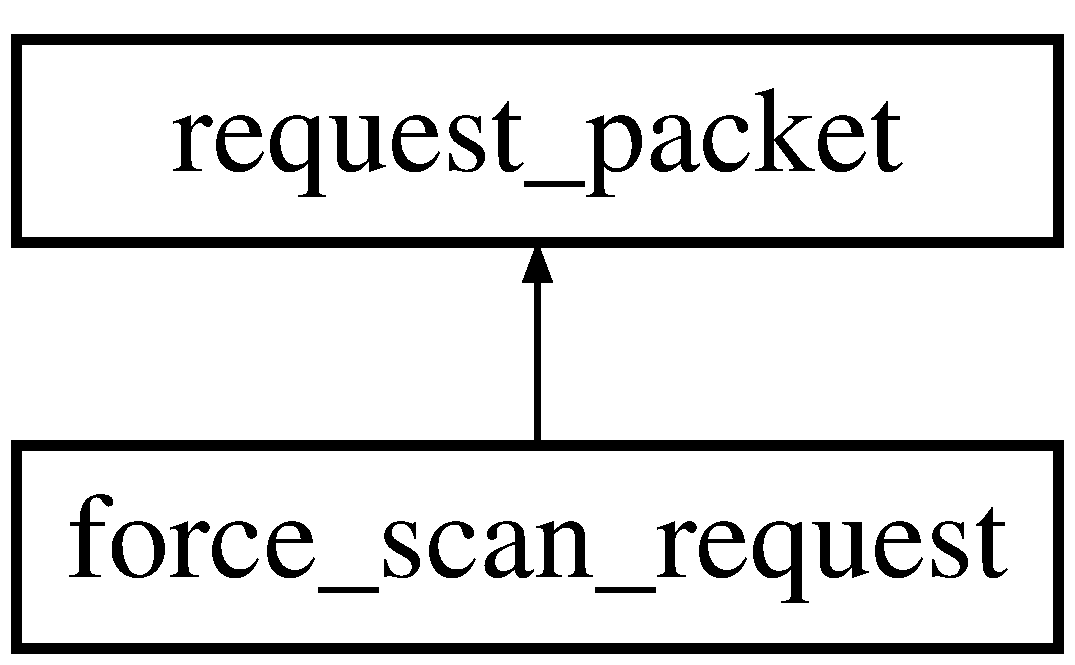
\includegraphics[height=2.000000cm]{structforce__scan__request}
\end{center}
\end{figure}
\subsection*{Public Member Functions}
\begin{DoxyCompactItemize}
\item 
\hyperlink{structforce__scan__request_ae9d2bfc20d451450b8e6c4febdf4a8ee}{force\-\_\-scan\-\_\-request} ()
\end{DoxyCompactItemize}
\subsection*{Additional Inherited Members}


\subsection{Constructor \& Destructor Documentation}
\hypertarget{structforce__scan__request_ae9d2bfc20d451450b8e6c4febdf4a8ee}{\index{force\-\_\-scan\-\_\-request@{force\-\_\-scan\-\_\-request}!force\-\_\-scan\-\_\-request@{force\-\_\-scan\-\_\-request}}
\index{force\-\_\-scan\-\_\-request@{force\-\_\-scan\-\_\-request}!force_scan_request@{force\-\_\-scan\-\_\-request}}
\subsubsection[{force\-\_\-scan\-\_\-request}]{\setlength{\rightskip}{0pt plus 5cm}force\-\_\-scan\-\_\-request\-::force\-\_\-scan\-\_\-request (
\begin{DoxyParamCaption}
{}
\end{DoxyParamCaption}
)\hspace{0.3cm}{\ttfamily [inline]}}}\label{structforce__scan__request_ae9d2bfc20d451450b8e6c4febdf4a8ee}


The documentation for this struct was generated from the following file\-:\begin{DoxyCompactItemize}
\item 
/home/dprandle/\-Documents/code/ctrlmod/include/\hyperlink{edrplidar__packets_8h}{edrplidar\-\_\-packets.\-h}\end{DoxyCompactItemize}

\hypertarget{structhealth__data__packet}{\section{health\-\_\-data\-\_\-packet Struct Reference}
\label{structhealth__data__packet}\index{health\-\_\-data\-\_\-packet@{health\-\_\-data\-\_\-packet}}
}


{\ttfamily \#include $<$edrplidar\-\_\-packets.\-h$>$}

Inheritance diagram for health\-\_\-data\-\_\-packet\-:\begin{figure}[H]
\begin{center}
\leavevmode
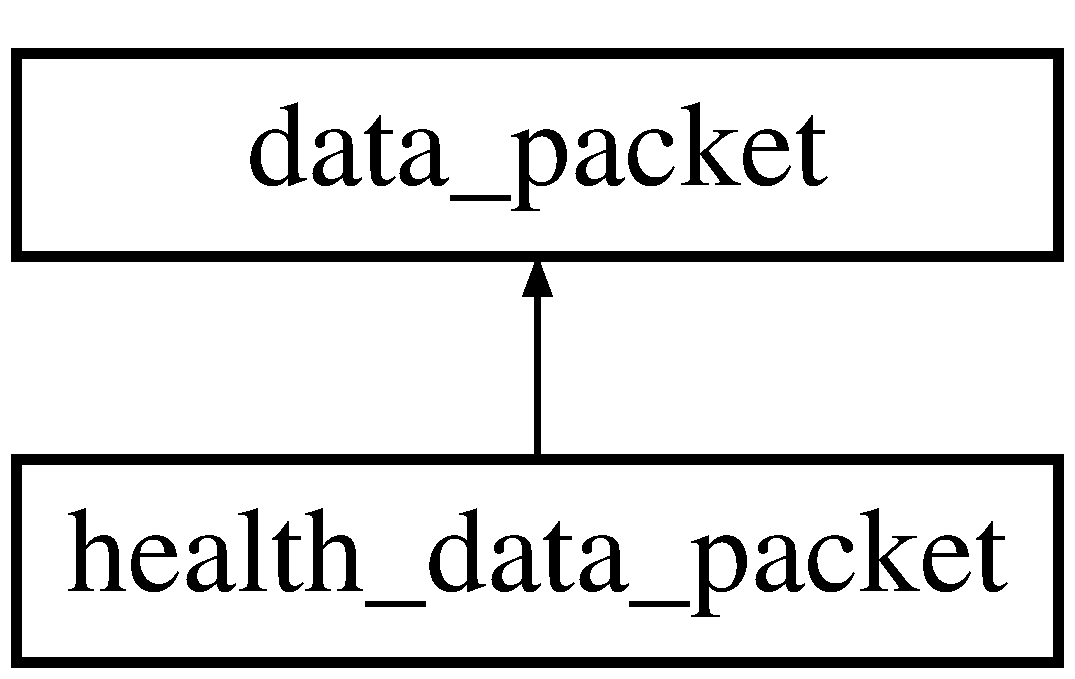
\includegraphics[height=2.000000cm]{structhealth__data__packet}
\end{center}
\end{figure}
\subsection*{Public Member Functions}
\begin{DoxyCompactItemize}
\item 
\hyperlink{structhealth__data__packet_a7cfb581955c8d81fc4b7a6aa98479553}{health\-\_\-data\-\_\-packet} ()
\item 
virtual std\-::string \hyperlink{structhealth__data__packet_a89e96e87bdcf2ecc52260a9d98e37995}{to\-String} ()
\item 
virtual std\-::string \hyperlink{structhealth__data__packet_abc386acf1fcf42086f1fc791d2718dff}{type} ()
\item 
virtual uint32\-\_\-t \hyperlink{structhealth__data__packet_a85329a68f718099b6cefcf65fab75077}{size} ()
\item 
virtual uint8\-\_\-t \& \hyperlink{structhealth__data__packet_aa96359c2b7100e17905e02c7ab68ca59}{operator\mbox{[}$\,$\mbox{]}} (uint32\-\_\-t index)
\item 
virtual uint8\-\_\-t $\ast$ \hyperlink{structhealth__data__packet_a8378ecf34528f77f6d50937c3ad02c8d}{dataptr} ()
\end{DoxyCompactItemize}
\subsection*{Static Public Member Functions}
\begin{DoxyCompactItemize}
\item 
static std\-::string \hyperlink{structhealth__data__packet_ab1066c5d4c3353c6d5175acef3b4fc9a}{Type} ()
\item 
static uint32\-\_\-t \hyperlink{structhealth__data__packet_a453e09780784287394585eedd99585f0}{Size} ()
\end{DoxyCompactItemize}
\subsection*{Public Attributes}
\begin{DoxyCompactItemize}
\item 
\begin{tabbing}
xx\=xx\=xx\=xx\=xx\=xx\=xx\=xx\=xx\=\kill
union \{\\
\>struct \{\\
\>\>uint8\_t \hyperlink{structhealth__data__packet_a866832727429756e4f03fcad5cf2e240}{status}\\
\>\>uint8\_t \hyperlink{structhealth__data__packet_a4bb1d8b54ac0d82856dfa030cd981f90}{error\_code7to0}\\
\>\>uint8\_t \hyperlink{structhealth__data__packet_a08f52ad70296c41370889f5f74f68908}{error\_code15to8}\\
\>\} \\
\>uint8\_t \hyperlink{structhealth__data__packet_a4039ceb368923f09e7d8e1cc7ada5760}{data} \mbox{[}3\mbox{]}\\
\}; \\

\end{tabbing}\end{DoxyCompactItemize}


\subsection{Constructor \& Destructor Documentation}
\hypertarget{structhealth__data__packet_a7cfb581955c8d81fc4b7a6aa98479553}{\index{health\-\_\-data\-\_\-packet@{health\-\_\-data\-\_\-packet}!health\-\_\-data\-\_\-packet@{health\-\_\-data\-\_\-packet}}
\index{health\-\_\-data\-\_\-packet@{health\-\_\-data\-\_\-packet}!health_data_packet@{health\-\_\-data\-\_\-packet}}
\subsubsection[{health\-\_\-data\-\_\-packet}]{\setlength{\rightskip}{0pt plus 5cm}health\-\_\-data\-\_\-packet\-::health\-\_\-data\-\_\-packet (
\begin{DoxyParamCaption}
{}
\end{DoxyParamCaption}
)}}\label{structhealth__data__packet_a7cfb581955c8d81fc4b7a6aa98479553}


\subsection{Member Function Documentation}
\hypertarget{structhealth__data__packet_a8378ecf34528f77f6d50937c3ad02c8d}{\index{health\-\_\-data\-\_\-packet@{health\-\_\-data\-\_\-packet}!dataptr@{dataptr}}
\index{dataptr@{dataptr}!health_data_packet@{health\-\_\-data\-\_\-packet}}
\subsubsection[{dataptr}]{\setlength{\rightskip}{0pt plus 5cm}virtual uint8\-\_\-t$\ast$ health\-\_\-data\-\_\-packet\-::dataptr (
\begin{DoxyParamCaption}
{}
\end{DoxyParamCaption}
)\hspace{0.3cm}{\ttfamily [inline]}, {\ttfamily [virtual]}}}\label{structhealth__data__packet_a8378ecf34528f77f6d50937c3ad02c8d}


Implements \hyperlink{structdata__packet_ac53dcca572fc7cf7d71ae21d5c785365}{data\-\_\-packet}.

\hypertarget{structhealth__data__packet_aa96359c2b7100e17905e02c7ab68ca59}{\index{health\-\_\-data\-\_\-packet@{health\-\_\-data\-\_\-packet}!operator\mbox{[}$\,$\mbox{]}@{operator[]}}
\index{operator\mbox{[}$\,$\mbox{]}@{operator[]}!health_data_packet@{health\-\_\-data\-\_\-packet}}
\subsubsection[{operator[]}]{\setlength{\rightskip}{0pt plus 5cm}virtual uint8\-\_\-t\& health\-\_\-data\-\_\-packet\-::operator\mbox{[}$\,$\mbox{]} (
\begin{DoxyParamCaption}
\item[{uint32\-\_\-t}]{index}
\end{DoxyParamCaption}
)\hspace{0.3cm}{\ttfamily [inline]}, {\ttfamily [virtual]}}}\label{structhealth__data__packet_aa96359c2b7100e17905e02c7ab68ca59}


Implements \hyperlink{structdata__packet_a8f0d95d4a7a7089b45cef14e45b0c21b}{data\-\_\-packet}.

\hypertarget{structhealth__data__packet_a85329a68f718099b6cefcf65fab75077}{\index{health\-\_\-data\-\_\-packet@{health\-\_\-data\-\_\-packet}!size@{size}}
\index{size@{size}!health_data_packet@{health\-\_\-data\-\_\-packet}}
\subsubsection[{size}]{\setlength{\rightskip}{0pt plus 5cm}virtual uint32\-\_\-t health\-\_\-data\-\_\-packet\-::size (
\begin{DoxyParamCaption}
{}
\end{DoxyParamCaption}
)\hspace{0.3cm}{\ttfamily [inline]}, {\ttfamily [virtual]}}}\label{structhealth__data__packet_a85329a68f718099b6cefcf65fab75077}


Implements \hyperlink{structdata__packet_ab5c9259a79cde0dc60d75135fe8464f6}{data\-\_\-packet}.

\hypertarget{structhealth__data__packet_a453e09780784287394585eedd99585f0}{\index{health\-\_\-data\-\_\-packet@{health\-\_\-data\-\_\-packet}!Size@{Size}}
\index{Size@{Size}!health_data_packet@{health\-\_\-data\-\_\-packet}}
\subsubsection[{Size}]{\setlength{\rightskip}{0pt plus 5cm}static uint32\-\_\-t health\-\_\-data\-\_\-packet\-::\-Size (
\begin{DoxyParamCaption}
{}
\end{DoxyParamCaption}
)\hspace{0.3cm}{\ttfamily [inline]}, {\ttfamily [static]}}}\label{structhealth__data__packet_a453e09780784287394585eedd99585f0}
\hypertarget{structhealth__data__packet_a89e96e87bdcf2ecc52260a9d98e37995}{\index{health\-\_\-data\-\_\-packet@{health\-\_\-data\-\_\-packet}!to\-String@{to\-String}}
\index{to\-String@{to\-String}!health_data_packet@{health\-\_\-data\-\_\-packet}}
\subsubsection[{to\-String}]{\setlength{\rightskip}{0pt plus 5cm}std\-::string health\-\_\-data\-\_\-packet\-::to\-String (
\begin{DoxyParamCaption}
{}
\end{DoxyParamCaption}
)\hspace{0.3cm}{\ttfamily [virtual]}}}\label{structhealth__data__packet_a89e96e87bdcf2ecc52260a9d98e37995}


Implements \hyperlink{structdata__packet_ad7ce179caef76c895bfc778862bc15ac}{data\-\_\-packet}.

\hypertarget{structhealth__data__packet_abc386acf1fcf42086f1fc791d2718dff}{\index{health\-\_\-data\-\_\-packet@{health\-\_\-data\-\_\-packet}!type@{type}}
\index{type@{type}!health_data_packet@{health\-\_\-data\-\_\-packet}}
\subsubsection[{type}]{\setlength{\rightskip}{0pt plus 5cm}virtual std\-::string health\-\_\-data\-\_\-packet\-::type (
\begin{DoxyParamCaption}
{}
\end{DoxyParamCaption}
)\hspace{0.3cm}{\ttfamily [inline]}, {\ttfamily [virtual]}}}\label{structhealth__data__packet_abc386acf1fcf42086f1fc791d2718dff}


Implements \hyperlink{structdata__packet_af0795581f2d57a8c14a88009da37aee1}{data\-\_\-packet}.

\hypertarget{structhealth__data__packet_ab1066c5d4c3353c6d5175acef3b4fc9a}{\index{health\-\_\-data\-\_\-packet@{health\-\_\-data\-\_\-packet}!Type@{Type}}
\index{Type@{Type}!health_data_packet@{health\-\_\-data\-\_\-packet}}
\subsubsection[{Type}]{\setlength{\rightskip}{0pt plus 5cm}static std\-::string health\-\_\-data\-\_\-packet\-::\-Type (
\begin{DoxyParamCaption}
{}
\end{DoxyParamCaption}
)\hspace{0.3cm}{\ttfamily [inline]}, {\ttfamily [static]}}}\label{structhealth__data__packet_ab1066c5d4c3353c6d5175acef3b4fc9a}


\subsection{Member Data Documentation}
\hypertarget{structhealth__data__packet_a41edefdf6f0636add1f38358092aa86a}{\subsubsection[{"@17}]{\setlength{\rightskip}{0pt plus 5cm}union \{ ... \} }}\label{structhealth__data__packet_a41edefdf6f0636add1f38358092aa86a}
\hypertarget{structhealth__data__packet_a4039ceb368923f09e7d8e1cc7ada5760}{\index{health\-\_\-data\-\_\-packet@{health\-\_\-data\-\_\-packet}!data@{data}}
\index{data@{data}!health_data_packet@{health\-\_\-data\-\_\-packet}}
\subsubsection[{data}]{\setlength{\rightskip}{0pt plus 5cm}uint8\-\_\-t health\-\_\-data\-\_\-packet\-::data\mbox{[}3\mbox{]}}}\label{structhealth__data__packet_a4039ceb368923f09e7d8e1cc7ada5760}
\hypertarget{structhealth__data__packet_a08f52ad70296c41370889f5f74f68908}{\index{health\-\_\-data\-\_\-packet@{health\-\_\-data\-\_\-packet}!error\-\_\-code15to8@{error\-\_\-code15to8}}
\index{error\-\_\-code15to8@{error\-\_\-code15to8}!health_data_packet@{health\-\_\-data\-\_\-packet}}
\subsubsection[{error\-\_\-code15to8}]{\setlength{\rightskip}{0pt plus 5cm}uint8\-\_\-t health\-\_\-data\-\_\-packet\-::error\-\_\-code15to8}}\label{structhealth__data__packet_a08f52ad70296c41370889f5f74f68908}
\hypertarget{structhealth__data__packet_a4bb1d8b54ac0d82856dfa030cd981f90}{\index{health\-\_\-data\-\_\-packet@{health\-\_\-data\-\_\-packet}!error\-\_\-code7to0@{error\-\_\-code7to0}}
\index{error\-\_\-code7to0@{error\-\_\-code7to0}!health_data_packet@{health\-\_\-data\-\_\-packet}}
\subsubsection[{error\-\_\-code7to0}]{\setlength{\rightskip}{0pt plus 5cm}uint8\-\_\-t health\-\_\-data\-\_\-packet\-::error\-\_\-code7to0}}\label{structhealth__data__packet_a4bb1d8b54ac0d82856dfa030cd981f90}
\hypertarget{structhealth__data__packet_a866832727429756e4f03fcad5cf2e240}{\index{health\-\_\-data\-\_\-packet@{health\-\_\-data\-\_\-packet}!status@{status}}
\index{status@{status}!health_data_packet@{health\-\_\-data\-\_\-packet}}
\subsubsection[{status}]{\setlength{\rightskip}{0pt plus 5cm}uint8\-\_\-t health\-\_\-data\-\_\-packet\-::status}}\label{structhealth__data__packet_a866832727429756e4f03fcad5cf2e240}


The documentation for this struct was generated from the following files\-:\begin{DoxyCompactItemize}
\item 
/home/dprandle/\-Documents/code/ctrlmod/include/\hyperlink{edrplidar__packets_8h}{edrplidar\-\_\-packets.\-h}\item 
/home/dprandle/\-Documents/code/ctrlmod/src/\hyperlink{edrplidar__packets_8cpp}{edrplidar\-\_\-packets.\-cpp}\end{DoxyCompactItemize}

\hypertarget{structinfo__data__packet}{\section{info\-\_\-data\-\_\-packet Struct Reference}
\label{structinfo__data__packet}\index{info\-\_\-data\-\_\-packet@{info\-\_\-data\-\_\-packet}}
}


{\ttfamily \#include $<$edrplidar\-\_\-packets.\-h$>$}

Inheritance diagram for info\-\_\-data\-\_\-packet\-:\begin{figure}[H]
\begin{center}
\leavevmode
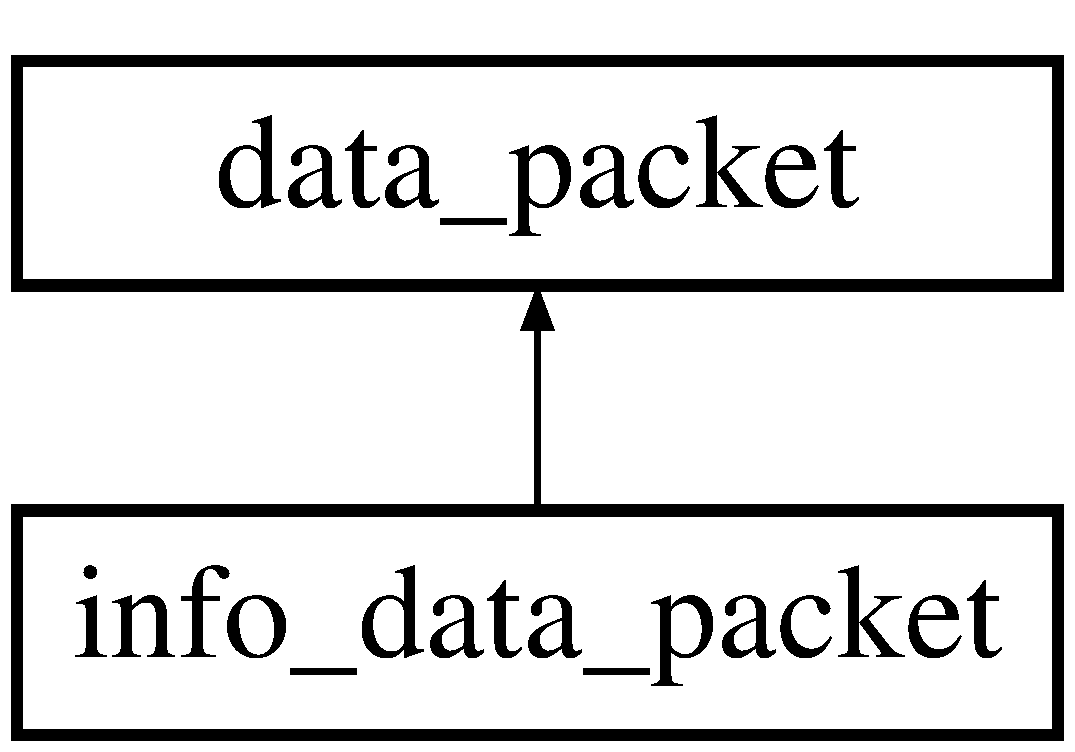
\includegraphics[height=2.000000cm]{structinfo__data__packet}
\end{center}
\end{figure}
\subsection*{Public Member Functions}
\begin{DoxyCompactItemize}
\item 
\hyperlink{structinfo__data__packet_afb9145aa395f640ad423624ea72730f5}{info\-\_\-data\-\_\-packet} ()
\item 
virtual std\-::string \hyperlink{structinfo__data__packet_a8c8b12d30a12b931740eb9c4cdc84315}{to\-String} ()
\item 
virtual std\-::string \hyperlink{structinfo__data__packet_a85dfeae92d487d55b6d57e95e0c2b662}{type} ()
\item 
virtual uint32\-\_\-t \hyperlink{structinfo__data__packet_a8852d00d040d27ba824dc333a8f66f44}{size} ()
\item 
virtual uint8\-\_\-t \& \hyperlink{structinfo__data__packet_a5a78a794ee110ed9bb4a4bb97d57f9f3}{operator\mbox{[}$\,$\mbox{]}} (uint32\-\_\-t index)
\item 
virtual uint8\-\_\-t $\ast$ \hyperlink{structinfo__data__packet_a2b730e457ee372ad1d40d4bbc22928cc}{dataptr} ()
\end{DoxyCompactItemize}
\subsection*{Static Public Member Functions}
\begin{DoxyCompactItemize}
\item 
static std\-::string \hyperlink{structinfo__data__packet_ad2f7f5bdfe8084400875436242fe9838}{Type} ()
\item 
static uint32\-\_\-t \hyperlink{structinfo__data__packet_a1dc781165e90e09e29fab25f6b9cfeb1}{Size} ()
\end{DoxyCompactItemize}
\subsection*{Public Attributes}
\begin{DoxyCompactItemize}
\item 
\begin{tabbing}
xx\=xx\=xx\=xx\=xx\=xx\=xx\=xx\=xx\=\kill
union \{\\
\>struct \{\\
\>\>uint8\_t \hyperlink{structinfo__data__packet_ab12797b480268b15712470dc9dd5cde9}{model}\\
\>\>uint8\_t \hyperlink{structinfo__data__packet_a8e8be6a19d3a61f23242f32383ad45a9}{firmware\_minor}\\
\>\>uint8\_t \hyperlink{structinfo__data__packet_ad4e1cf4e56610f97c2a652883f316d3a}{firmware\_major}\\
\>\>uint8\_t \hyperlink{structinfo__data__packet_a561357c591a36153ba2db03416d211a6}{hardware}\\
\>\>uint8\_t \hyperlink{structinfo__data__packet_a17f0e185c469b1502816ccccc371165b}{serialnumber} \mbox{[}16\mbox{]}\\
\>\} \\
\>uint8\_t \hyperlink{structinfo__data__packet_aadb324ab652eb4626f43f664bda87d22}{data} \mbox{[}20\mbox{]}\\
\}; \\

\end{tabbing}\end{DoxyCompactItemize}


\subsection{Constructor \& Destructor Documentation}
\hypertarget{structinfo__data__packet_afb9145aa395f640ad423624ea72730f5}{\index{info\-\_\-data\-\_\-packet@{info\-\_\-data\-\_\-packet}!info\-\_\-data\-\_\-packet@{info\-\_\-data\-\_\-packet}}
\index{info\-\_\-data\-\_\-packet@{info\-\_\-data\-\_\-packet}!info_data_packet@{info\-\_\-data\-\_\-packet}}
\subsubsection[{info\-\_\-data\-\_\-packet}]{\setlength{\rightskip}{0pt plus 5cm}info\-\_\-data\-\_\-packet\-::info\-\_\-data\-\_\-packet (
\begin{DoxyParamCaption}
{}
\end{DoxyParamCaption}
)}}\label{structinfo__data__packet_afb9145aa395f640ad423624ea72730f5}


\subsection{Member Function Documentation}
\hypertarget{structinfo__data__packet_a2b730e457ee372ad1d40d4bbc22928cc}{\index{info\-\_\-data\-\_\-packet@{info\-\_\-data\-\_\-packet}!dataptr@{dataptr}}
\index{dataptr@{dataptr}!info_data_packet@{info\-\_\-data\-\_\-packet}}
\subsubsection[{dataptr}]{\setlength{\rightskip}{0pt plus 5cm}virtual uint8\-\_\-t$\ast$ info\-\_\-data\-\_\-packet\-::dataptr (
\begin{DoxyParamCaption}
{}
\end{DoxyParamCaption}
)\hspace{0.3cm}{\ttfamily [inline]}, {\ttfamily [virtual]}}}\label{structinfo__data__packet_a2b730e457ee372ad1d40d4bbc22928cc}


Implements \hyperlink{structdata__packet_ac53dcca572fc7cf7d71ae21d5c785365}{data\-\_\-packet}.

\hypertarget{structinfo__data__packet_a5a78a794ee110ed9bb4a4bb97d57f9f3}{\index{info\-\_\-data\-\_\-packet@{info\-\_\-data\-\_\-packet}!operator\mbox{[}$\,$\mbox{]}@{operator[]}}
\index{operator\mbox{[}$\,$\mbox{]}@{operator[]}!info_data_packet@{info\-\_\-data\-\_\-packet}}
\subsubsection[{operator[]}]{\setlength{\rightskip}{0pt plus 5cm}virtual uint8\-\_\-t\& info\-\_\-data\-\_\-packet\-::operator\mbox{[}$\,$\mbox{]} (
\begin{DoxyParamCaption}
\item[{uint32\-\_\-t}]{index}
\end{DoxyParamCaption}
)\hspace{0.3cm}{\ttfamily [inline]}, {\ttfamily [virtual]}}}\label{structinfo__data__packet_a5a78a794ee110ed9bb4a4bb97d57f9f3}


Implements \hyperlink{structdata__packet_a8f0d95d4a7a7089b45cef14e45b0c21b}{data\-\_\-packet}.

\hypertarget{structinfo__data__packet_a8852d00d040d27ba824dc333a8f66f44}{\index{info\-\_\-data\-\_\-packet@{info\-\_\-data\-\_\-packet}!size@{size}}
\index{size@{size}!info_data_packet@{info\-\_\-data\-\_\-packet}}
\subsubsection[{size}]{\setlength{\rightskip}{0pt plus 5cm}virtual uint32\-\_\-t info\-\_\-data\-\_\-packet\-::size (
\begin{DoxyParamCaption}
{}
\end{DoxyParamCaption}
)\hspace{0.3cm}{\ttfamily [inline]}, {\ttfamily [virtual]}}}\label{structinfo__data__packet_a8852d00d040d27ba824dc333a8f66f44}


Implements \hyperlink{structdata__packet_ab5c9259a79cde0dc60d75135fe8464f6}{data\-\_\-packet}.

\hypertarget{structinfo__data__packet_a1dc781165e90e09e29fab25f6b9cfeb1}{\index{info\-\_\-data\-\_\-packet@{info\-\_\-data\-\_\-packet}!Size@{Size}}
\index{Size@{Size}!info_data_packet@{info\-\_\-data\-\_\-packet}}
\subsubsection[{Size}]{\setlength{\rightskip}{0pt plus 5cm}static uint32\-\_\-t info\-\_\-data\-\_\-packet\-::\-Size (
\begin{DoxyParamCaption}
{}
\end{DoxyParamCaption}
)\hspace{0.3cm}{\ttfamily [inline]}, {\ttfamily [static]}}}\label{structinfo__data__packet_a1dc781165e90e09e29fab25f6b9cfeb1}
\hypertarget{structinfo__data__packet_a8c8b12d30a12b931740eb9c4cdc84315}{\index{info\-\_\-data\-\_\-packet@{info\-\_\-data\-\_\-packet}!to\-String@{to\-String}}
\index{to\-String@{to\-String}!info_data_packet@{info\-\_\-data\-\_\-packet}}
\subsubsection[{to\-String}]{\setlength{\rightskip}{0pt plus 5cm}std\-::string info\-\_\-data\-\_\-packet\-::to\-String (
\begin{DoxyParamCaption}
{}
\end{DoxyParamCaption}
)\hspace{0.3cm}{\ttfamily [virtual]}}}\label{structinfo__data__packet_a8c8b12d30a12b931740eb9c4cdc84315}


Implements \hyperlink{structdata__packet_ad7ce179caef76c895bfc778862bc15ac}{data\-\_\-packet}.

\hypertarget{structinfo__data__packet_a85dfeae92d487d55b6d57e95e0c2b662}{\index{info\-\_\-data\-\_\-packet@{info\-\_\-data\-\_\-packet}!type@{type}}
\index{type@{type}!info_data_packet@{info\-\_\-data\-\_\-packet}}
\subsubsection[{type}]{\setlength{\rightskip}{0pt plus 5cm}virtual std\-::string info\-\_\-data\-\_\-packet\-::type (
\begin{DoxyParamCaption}
{}
\end{DoxyParamCaption}
)\hspace{0.3cm}{\ttfamily [inline]}, {\ttfamily [virtual]}}}\label{structinfo__data__packet_a85dfeae92d487d55b6d57e95e0c2b662}


Implements \hyperlink{structdata__packet_af0795581f2d57a8c14a88009da37aee1}{data\-\_\-packet}.

\hypertarget{structinfo__data__packet_ad2f7f5bdfe8084400875436242fe9838}{\index{info\-\_\-data\-\_\-packet@{info\-\_\-data\-\_\-packet}!Type@{Type}}
\index{Type@{Type}!info_data_packet@{info\-\_\-data\-\_\-packet}}
\subsubsection[{Type}]{\setlength{\rightskip}{0pt plus 5cm}static std\-::string info\-\_\-data\-\_\-packet\-::\-Type (
\begin{DoxyParamCaption}
{}
\end{DoxyParamCaption}
)\hspace{0.3cm}{\ttfamily [inline]}, {\ttfamily [static]}}}\label{structinfo__data__packet_ad2f7f5bdfe8084400875436242fe9838}


\subsection{Member Data Documentation}
\hypertarget{structinfo__data__packet_a2c2f67a49766988f454c0bd33c558574}{\subsubsection[{"@21}]{\setlength{\rightskip}{0pt plus 5cm}union \{ ... \} }}\label{structinfo__data__packet_a2c2f67a49766988f454c0bd33c558574}
\hypertarget{structinfo__data__packet_aadb324ab652eb4626f43f664bda87d22}{\index{info\-\_\-data\-\_\-packet@{info\-\_\-data\-\_\-packet}!data@{data}}
\index{data@{data}!info_data_packet@{info\-\_\-data\-\_\-packet}}
\subsubsection[{data}]{\setlength{\rightskip}{0pt plus 5cm}uint8\-\_\-t info\-\_\-data\-\_\-packet\-::data\mbox{[}20\mbox{]}}}\label{structinfo__data__packet_aadb324ab652eb4626f43f664bda87d22}
\hypertarget{structinfo__data__packet_ad4e1cf4e56610f97c2a652883f316d3a}{\index{info\-\_\-data\-\_\-packet@{info\-\_\-data\-\_\-packet}!firmware\-\_\-major@{firmware\-\_\-major}}
\index{firmware\-\_\-major@{firmware\-\_\-major}!info_data_packet@{info\-\_\-data\-\_\-packet}}
\subsubsection[{firmware\-\_\-major}]{\setlength{\rightskip}{0pt plus 5cm}uint8\-\_\-t info\-\_\-data\-\_\-packet\-::firmware\-\_\-major}}\label{structinfo__data__packet_ad4e1cf4e56610f97c2a652883f316d3a}
\hypertarget{structinfo__data__packet_a8e8be6a19d3a61f23242f32383ad45a9}{\index{info\-\_\-data\-\_\-packet@{info\-\_\-data\-\_\-packet}!firmware\-\_\-minor@{firmware\-\_\-minor}}
\index{firmware\-\_\-minor@{firmware\-\_\-minor}!info_data_packet@{info\-\_\-data\-\_\-packet}}
\subsubsection[{firmware\-\_\-minor}]{\setlength{\rightskip}{0pt plus 5cm}uint8\-\_\-t info\-\_\-data\-\_\-packet\-::firmware\-\_\-minor}}\label{structinfo__data__packet_a8e8be6a19d3a61f23242f32383ad45a9}
\hypertarget{structinfo__data__packet_a561357c591a36153ba2db03416d211a6}{\index{info\-\_\-data\-\_\-packet@{info\-\_\-data\-\_\-packet}!hardware@{hardware}}
\index{hardware@{hardware}!info_data_packet@{info\-\_\-data\-\_\-packet}}
\subsubsection[{hardware}]{\setlength{\rightskip}{0pt plus 5cm}uint8\-\_\-t info\-\_\-data\-\_\-packet\-::hardware}}\label{structinfo__data__packet_a561357c591a36153ba2db03416d211a6}
\hypertarget{structinfo__data__packet_ab12797b480268b15712470dc9dd5cde9}{\index{info\-\_\-data\-\_\-packet@{info\-\_\-data\-\_\-packet}!model@{model}}
\index{model@{model}!info_data_packet@{info\-\_\-data\-\_\-packet}}
\subsubsection[{model}]{\setlength{\rightskip}{0pt plus 5cm}uint8\-\_\-t info\-\_\-data\-\_\-packet\-::model}}\label{structinfo__data__packet_ab12797b480268b15712470dc9dd5cde9}
\hypertarget{structinfo__data__packet_a17f0e185c469b1502816ccccc371165b}{\index{info\-\_\-data\-\_\-packet@{info\-\_\-data\-\_\-packet}!serialnumber@{serialnumber}}
\index{serialnumber@{serialnumber}!info_data_packet@{info\-\_\-data\-\_\-packet}}
\subsubsection[{serialnumber}]{\setlength{\rightskip}{0pt plus 5cm}uint8\-\_\-t info\-\_\-data\-\_\-packet\-::serialnumber\mbox{[}16\mbox{]}}}\label{structinfo__data__packet_a17f0e185c469b1502816ccccc371165b}


The documentation for this struct was generated from the following files\-:\begin{DoxyCompactItemize}
\item 
/home/dprandle/\-Documents/code/ctrlmod/include/\hyperlink{edrplidar__packets_8h}{edrplidar\-\_\-packets.\-h}\item 
/home/dprandle/\-Documents/code/ctrlmod/src/\hyperlink{edrplidar__packets_8cpp}{edrplidar\-\_\-packets.\-cpp}\end{DoxyCompactItemize}

\hypertarget{structinstruction__callback}{\section{instruction\-\_\-callback Struct Reference}
\label{structinstruction__callback}\index{instruction\-\_\-callback@{instruction\-\_\-callback}}
}


{\ttfamily \#include $<$ednavsystem.\-h$>$}

Inheritance diagram for instruction\-\_\-callback\-:\begin{figure}[H]
\begin{center}
\leavevmode
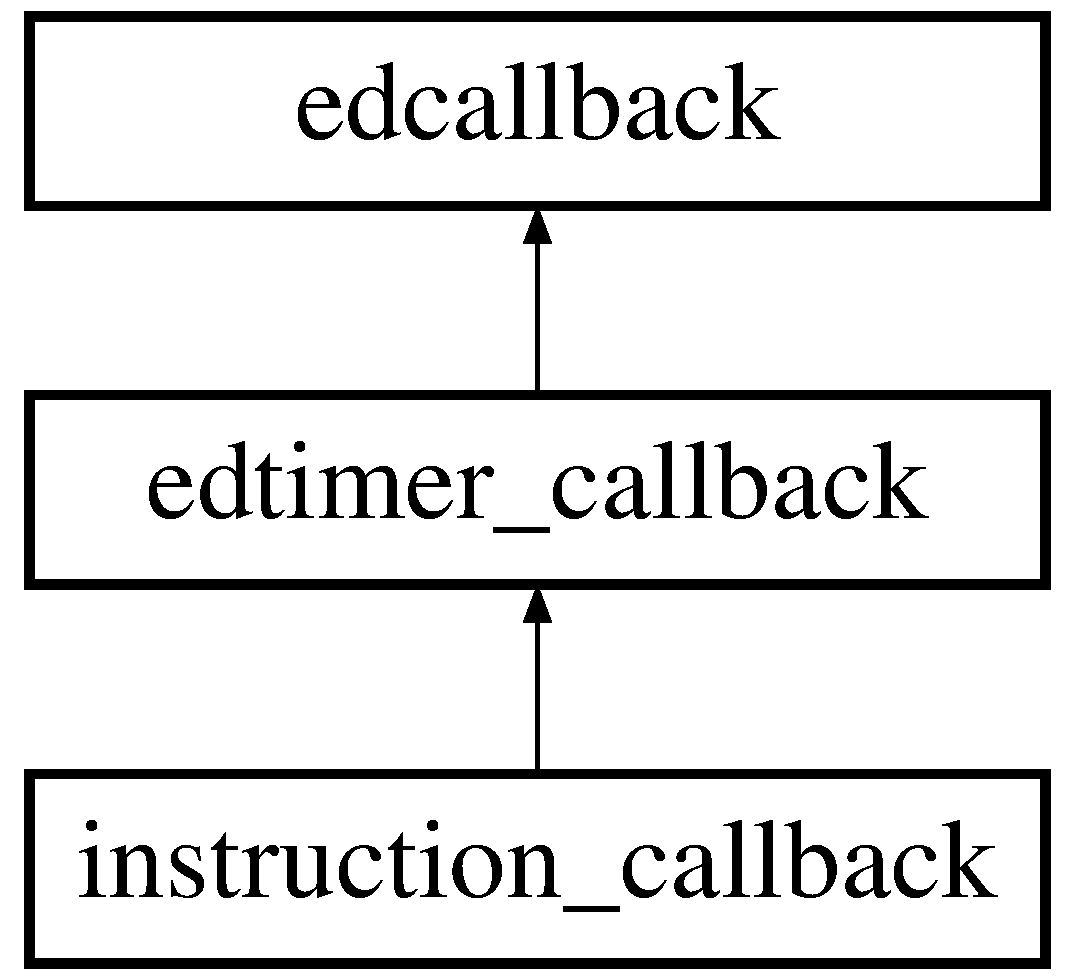
\includegraphics[height=3.000000cm]{structinstruction__callback}
\end{center}
\end{figure}
\subsection*{Public Member Functions}
\begin{DoxyCompactItemize}
\item 
\hyperlink{structinstruction__callback_a718fc48b66cbe5b8acac6202e9ef5b2c}{instruction\-\_\-callback} (\hyperlink{classednav__system}{ednav\-\_\-system} $\ast$system)
\item 
void \hyperlink{structinstruction__callback_a74abfad8ac25461bb99e11fba10516c2}{exec} ()
\end{DoxyCompactItemize}
\subsection*{Public Attributes}
\begin{DoxyCompactItemize}
\item 
\hyperlink{classednav__system}{ednav\-\_\-system} $\ast$ \hyperlink{structinstruction__callback_a5d86b6edbb2d2a9425c42b4c021138e6}{m\-\_\-nav\-\_\-sys}
\end{DoxyCompactItemize}


\subsection{Constructor \& Destructor Documentation}
\hypertarget{structinstruction__callback_a718fc48b66cbe5b8acac6202e9ef5b2c}{\index{instruction\-\_\-callback@{instruction\-\_\-callback}!instruction\-\_\-callback@{instruction\-\_\-callback}}
\index{instruction\-\_\-callback@{instruction\-\_\-callback}!instruction_callback@{instruction\-\_\-callback}}
\subsubsection[{instruction\-\_\-callback}]{\setlength{\rightskip}{0pt plus 5cm}instruction\-\_\-callback\-::instruction\-\_\-callback (
\begin{DoxyParamCaption}
\item[{{\bf ednav\-\_\-system} $\ast$}]{system}
\end{DoxyParamCaption}
)\hspace{0.3cm}{\ttfamily [inline]}}}\label{structinstruction__callback_a718fc48b66cbe5b8acac6202e9ef5b2c}


\subsection{Member Function Documentation}
\hypertarget{structinstruction__callback_a74abfad8ac25461bb99e11fba10516c2}{\index{instruction\-\_\-callback@{instruction\-\_\-callback}!exec@{exec}}
\index{exec@{exec}!instruction_callback@{instruction\-\_\-callback}}
\subsubsection[{exec}]{\setlength{\rightskip}{0pt plus 5cm}void instruction\-\_\-callback\-::exec (
\begin{DoxyParamCaption}
{}
\end{DoxyParamCaption}
)\hspace{0.3cm}{\ttfamily [virtual]}}}\label{structinstruction__callback_a74abfad8ac25461bb99e11fba10516c2}


Implements \hyperlink{structedcallback_ab8003af2178e58a94f53370b1f48a313}{edcallback}.



\subsection{Member Data Documentation}
\hypertarget{structinstruction__callback_a5d86b6edbb2d2a9425c42b4c021138e6}{\index{instruction\-\_\-callback@{instruction\-\_\-callback}!m\-\_\-nav\-\_\-sys@{m\-\_\-nav\-\_\-sys}}
\index{m\-\_\-nav\-\_\-sys@{m\-\_\-nav\-\_\-sys}!instruction_callback@{instruction\-\_\-callback}}
\subsubsection[{m\-\_\-nav\-\_\-sys}]{\setlength{\rightskip}{0pt plus 5cm}{\bf ednav\-\_\-system}$\ast$ instruction\-\_\-callback\-::m\-\_\-nav\-\_\-sys}}\label{structinstruction__callback_a5d86b6edbb2d2a9425c42b4c021138e6}


The documentation for this struct was generated from the following files\-:\begin{DoxyCompactItemize}
\item 
/home/dprandle/\-Documents/code/ctrlmod/include/\hyperlink{ednavsystem_8h}{ednavsystem.\-h}\item 
/home/dprandle/\-Documents/code/ctrlmod/src/\hyperlink{ednavsystem_8cpp}{ednavsystem.\-cpp}\end{DoxyCompactItemize}

\hypertarget{structnav__message}{\section{nav\-\_\-message Struct Reference}
\label{structnav__message}\index{nav\-\_\-message@{nav\-\_\-message}}
}


{\ttfamily \#include $<$edmessage.\-h$>$}

Inheritance diagram for nav\-\_\-message\-:\begin{figure}[H]
\begin{center}
\leavevmode
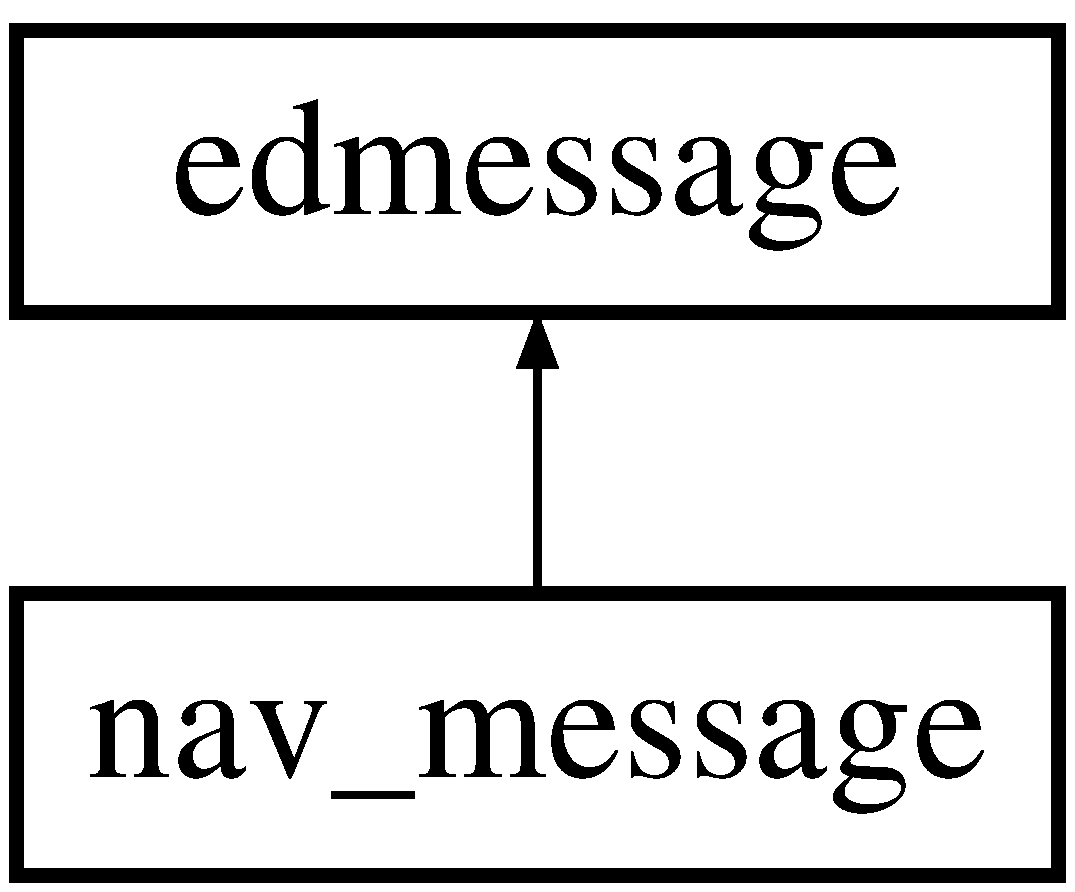
\includegraphics[height=2.000000cm]{structnav__message}
\end{center}
\end{figure}
\subsection*{Public Member Functions}
\begin{DoxyCompactItemize}
\item 
uint32\-\_\-t \hyperlink{structnav__message_a0d38fb1c8e8c376f54fe75e75a172983}{size} ()
\item 
std\-::string \hyperlink{structnav__message_a71d65e9c6328a4f9d2393d010f5fe873}{type} ()
\end{DoxyCompactItemize}
\subsection*{Static Public Member Functions}
\begin{DoxyCompactItemize}
\item 
static std\-::string \hyperlink{structnav__message_af310709544394bf9ca4c09a8f0039c00}{Type} ()
\end{DoxyCompactItemize}
\subsection*{Public Attributes}
\begin{DoxyCompactItemize}
\item 
\begin{tabbing}
xx\=xx\=xx\=xx\=xx\=xx\=xx\=xx\=xx\=\kill
union \{\\
\>struct \{\\
\>\>int16\_t \hyperlink{structnav__message_a32fbab7c09ee796640dd6e6748702576}{throttle}\\
\>\>int16\_t \hyperlink{structnav__message_af6064924eb9301edcf3d8bfbe6443bb3}{pitch}\\
\>\>int16\_t \hyperlink{structnav__message_a5a9f998f05f761c0ef2ecc4f421e56fa}{roll}\\
\>\>int16\_t \hyperlink{structnav__message_acb15f6079e91e8d5bf14be16293da809}{yaw}\\
\>\>double \hyperlink{structnav__message_a8825929bbd4efd96ec1498bf89194e66}{rvec\_raw} \mbox{[}2\mbox{]}\\
\>\>double \hyperlink{structnav__message_ae77c9ce12a1b1d950b9c4e7a8eb95ffb}{rvec\_corrected} \mbox{[}2\mbox{]}\\
\>\} \\
\>uint8\_t \hyperlink{structnav__message_aefc019e701a7c34f352fca4f15f54e6f}{data} \mbox{[}40\mbox{]}\\
\}; \\

\end{tabbing}\end{DoxyCompactItemize}


\subsection{Member Function Documentation}
\hypertarget{structnav__message_a0d38fb1c8e8c376f54fe75e75a172983}{\index{nav\-\_\-message@{nav\-\_\-message}!size@{size}}
\index{size@{size}!nav_message@{nav\-\_\-message}}
\subsubsection[{size}]{\setlength{\rightskip}{0pt plus 5cm}uint32\-\_\-t nav\-\_\-message\-::size (
\begin{DoxyParamCaption}
{}
\end{DoxyParamCaption}
)\hspace{0.3cm}{\ttfamily [inline]}}}\label{structnav__message_a0d38fb1c8e8c376f54fe75e75a172983}
\hypertarget{structnav__message_a71d65e9c6328a4f9d2393d010f5fe873}{\index{nav\-\_\-message@{nav\-\_\-message}!type@{type}}
\index{type@{type}!nav_message@{nav\-\_\-message}}
\subsubsection[{type}]{\setlength{\rightskip}{0pt plus 5cm}std\-::string nav\-\_\-message\-::type (
\begin{DoxyParamCaption}
{}
\end{DoxyParamCaption}
)\hspace{0.3cm}{\ttfamily [inline]}, {\ttfamily [virtual]}}}\label{structnav__message_a71d65e9c6328a4f9d2393d010f5fe873}


Implements \hyperlink{structedmessage_ac888cf8e570a4aa9bea30a4c4fcdcc30}{edmessage}.

\hypertarget{structnav__message_af310709544394bf9ca4c09a8f0039c00}{\index{nav\-\_\-message@{nav\-\_\-message}!Type@{Type}}
\index{Type@{Type}!nav_message@{nav\-\_\-message}}
\subsubsection[{Type}]{\setlength{\rightskip}{0pt plus 5cm}static std\-::string nav\-\_\-message\-::\-Type (
\begin{DoxyParamCaption}
{}
\end{DoxyParamCaption}
)\hspace{0.3cm}{\ttfamily [inline]}, {\ttfamily [static]}}}\label{structnav__message_af310709544394bf9ca4c09a8f0039c00}


\subsection{Member Data Documentation}
\hypertarget{structnav__message_aa5a224ab5d7821bb000c2085c71a13ba}{\subsubsection[{"@9}]{\setlength{\rightskip}{0pt plus 5cm}union \{ ... \} }}\label{structnav__message_aa5a224ab5d7821bb000c2085c71a13ba}
\hypertarget{structnav__message_aefc019e701a7c34f352fca4f15f54e6f}{\index{nav\-\_\-message@{nav\-\_\-message}!data@{data}}
\index{data@{data}!nav_message@{nav\-\_\-message}}
\subsubsection[{data}]{\setlength{\rightskip}{0pt plus 5cm}uint8\-\_\-t nav\-\_\-message\-::data\mbox{[}40\mbox{]}}}\label{structnav__message_aefc019e701a7c34f352fca4f15f54e6f}
\hypertarget{structnav__message_af6064924eb9301edcf3d8bfbe6443bb3}{\index{nav\-\_\-message@{nav\-\_\-message}!pitch@{pitch}}
\index{pitch@{pitch}!nav_message@{nav\-\_\-message}}
\subsubsection[{pitch}]{\setlength{\rightskip}{0pt plus 5cm}int16\-\_\-t nav\-\_\-message\-::pitch}}\label{structnav__message_af6064924eb9301edcf3d8bfbe6443bb3}
\hypertarget{structnav__message_a5a9f998f05f761c0ef2ecc4f421e56fa}{\index{nav\-\_\-message@{nav\-\_\-message}!roll@{roll}}
\index{roll@{roll}!nav_message@{nav\-\_\-message}}
\subsubsection[{roll}]{\setlength{\rightskip}{0pt plus 5cm}int16\-\_\-t nav\-\_\-message\-::roll}}\label{structnav__message_a5a9f998f05f761c0ef2ecc4f421e56fa}
\hypertarget{structnav__message_ae77c9ce12a1b1d950b9c4e7a8eb95ffb}{\index{nav\-\_\-message@{nav\-\_\-message}!rvec\-\_\-corrected@{rvec\-\_\-corrected}}
\index{rvec\-\_\-corrected@{rvec\-\_\-corrected}!nav_message@{nav\-\_\-message}}
\subsubsection[{rvec\-\_\-corrected}]{\setlength{\rightskip}{0pt plus 5cm}double nav\-\_\-message\-::rvec\-\_\-corrected\mbox{[}2\mbox{]}}}\label{structnav__message_ae77c9ce12a1b1d950b9c4e7a8eb95ffb}
\hypertarget{structnav__message_a8825929bbd4efd96ec1498bf89194e66}{\index{nav\-\_\-message@{nav\-\_\-message}!rvec\-\_\-raw@{rvec\-\_\-raw}}
\index{rvec\-\_\-raw@{rvec\-\_\-raw}!nav_message@{nav\-\_\-message}}
\subsubsection[{rvec\-\_\-raw}]{\setlength{\rightskip}{0pt plus 5cm}double nav\-\_\-message\-::rvec\-\_\-raw\mbox{[}2\mbox{]}}}\label{structnav__message_a8825929bbd4efd96ec1498bf89194e66}
\hypertarget{structnav__message_a32fbab7c09ee796640dd6e6748702576}{\index{nav\-\_\-message@{nav\-\_\-message}!throttle@{throttle}}
\index{throttle@{throttle}!nav_message@{nav\-\_\-message}}
\subsubsection[{throttle}]{\setlength{\rightskip}{0pt plus 5cm}int16\-\_\-t nav\-\_\-message\-::throttle}}\label{structnav__message_a32fbab7c09ee796640dd6e6748702576}
\hypertarget{structnav__message_acb15f6079e91e8d5bf14be16293da809}{\index{nav\-\_\-message@{nav\-\_\-message}!yaw@{yaw}}
\index{yaw@{yaw}!nav_message@{nav\-\_\-message}}
\subsubsection[{yaw}]{\setlength{\rightskip}{0pt plus 5cm}int16\-\_\-t nav\-\_\-message\-::yaw}}\label{structnav__message_acb15f6079e91e8d5bf14be16293da809}


The documentation for this struct was generated from the following file\-:\begin{DoxyCompactItemize}
\item 
/home/dprandle/\-Documents/code/ctrlmod/include/\hyperlink{edmessage_8h}{edmessage.\-h}\end{DoxyCompactItemize}

\hypertarget{structnav__system__request}{\section{nav\-\_\-system\-\_\-request Struct Reference}
\label{structnav__system__request}\index{nav\-\_\-system\-\_\-request@{nav\-\_\-system\-\_\-request}}
}


{\ttfamily \#include $<$edmessage.\-h$>$}

Inheritance diagram for nav\-\_\-system\-\_\-request\-:\begin{figure}[H]
\begin{center}
\leavevmode
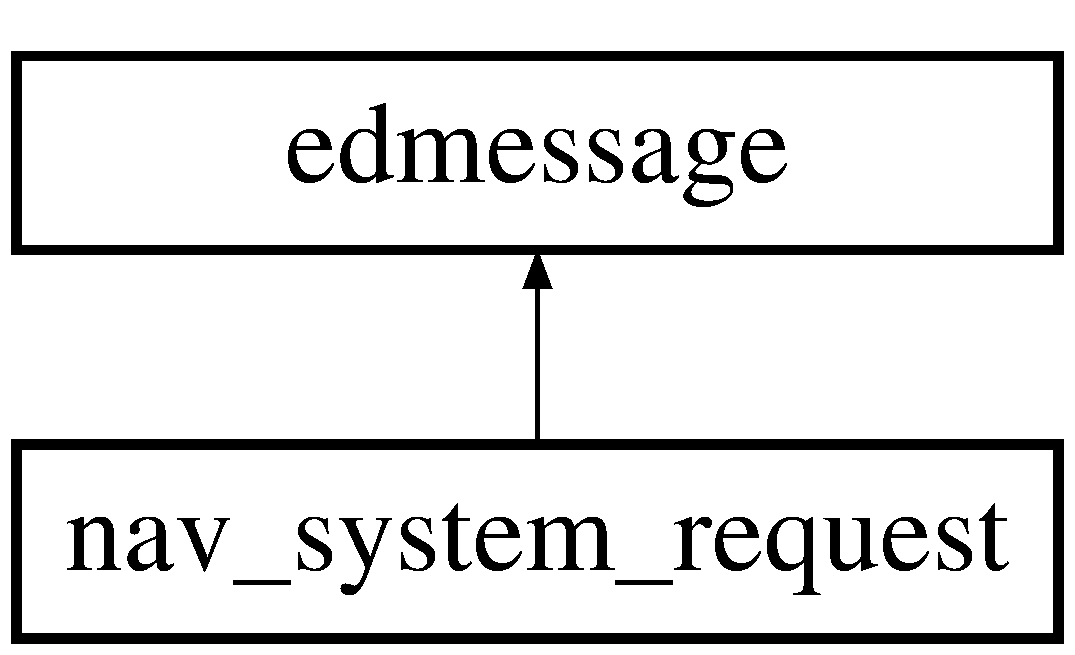
\includegraphics[height=2.000000cm]{structnav__system__request}
\end{center}
\end{figure}
\subsection*{Public Member Functions}
\begin{DoxyCompactItemize}
\item 
virtual std\-::string \hyperlink{structnav__system__request_aea068f2cdc3e36680b870c0acdfdd111}{type} ()
\end{DoxyCompactItemize}
\subsection*{Static Public Member Functions}
\begin{DoxyCompactItemize}
\item 
static std\-::string \hyperlink{structnav__system__request_a97cb1df7141c49f62ee8c244af217823}{Type} ()
\end{DoxyCompactItemize}
\subsection*{Public Attributes}
\begin{DoxyCompactItemize}
\item 
\hyperlink{nsmath_8h_a14bb8a4a0fefc0be4fae32fc59a07362}{vec3} \hyperlink{structnav__system__request_afaa3f6d1981d08595a44077e94f0ead5}{pid}
\item 
double \hyperlink{structnav__system__request_a168509fedd9762343017c1770812e93a}{ramp\-\_\-limit}
\item 
\hyperlink{nsmath_8h_ac5a07faf541e87fb0b7dbb6475cb9afb}{vec2} \hyperlink{structnav__system__request_a566b2891814edabd1e6d73fc2317a016}{bias\-\_\-vec}
\item 
double \hyperlink{structnav__system__request_a3734a6a3991044e9f18e63d1f8405293}{g\-\_\-factor}
\item 
double \hyperlink{structnav__system__request_a98b66505eb818bc1b8b0589629db6774}{bias\-\_\-threshold\-\_\-dist}
\item 
bool \hyperlink{structnav__system__request_abbf882832304276ef120aef92e62d011}{complex\-\_\-der}
\item 
bool \hyperlink{structnav__system__request_a8d92b7152b52f5242bd2530e5a78e595}{anti\-\_\-reset\-\_\-winding}
\item 
bool \hyperlink{structnav__system__request_a37812000ff825a1a389e4ea00c8daa52}{threshold\-\_\-dropout}
\end{DoxyCompactItemize}


\subsection{Member Function Documentation}
\hypertarget{structnav__system__request_aea068f2cdc3e36680b870c0acdfdd111}{\index{nav\-\_\-system\-\_\-request@{nav\-\_\-system\-\_\-request}!type@{type}}
\index{type@{type}!nav_system_request@{nav\-\_\-system\-\_\-request}}
\subsubsection[{type}]{\setlength{\rightskip}{0pt plus 5cm}virtual std\-::string nav\-\_\-system\-\_\-request\-::type (
\begin{DoxyParamCaption}
{}
\end{DoxyParamCaption}
)\hspace{0.3cm}{\ttfamily [inline]}, {\ttfamily [virtual]}}}\label{structnav__system__request_aea068f2cdc3e36680b870c0acdfdd111}


Implements \hyperlink{structedmessage_ac888cf8e570a4aa9bea30a4c4fcdcc30}{edmessage}.

\hypertarget{structnav__system__request_a97cb1df7141c49f62ee8c244af217823}{\index{nav\-\_\-system\-\_\-request@{nav\-\_\-system\-\_\-request}!Type@{Type}}
\index{Type@{Type}!nav_system_request@{nav\-\_\-system\-\_\-request}}
\subsubsection[{Type}]{\setlength{\rightskip}{0pt plus 5cm}static std\-::string nav\-\_\-system\-\_\-request\-::\-Type (
\begin{DoxyParamCaption}
{}
\end{DoxyParamCaption}
)\hspace{0.3cm}{\ttfamily [inline]}, {\ttfamily [static]}}}\label{structnav__system__request_a97cb1df7141c49f62ee8c244af217823}


\subsection{Member Data Documentation}
\hypertarget{structnav__system__request_a8d92b7152b52f5242bd2530e5a78e595}{\index{nav\-\_\-system\-\_\-request@{nav\-\_\-system\-\_\-request}!anti\-\_\-reset\-\_\-winding@{anti\-\_\-reset\-\_\-winding}}
\index{anti\-\_\-reset\-\_\-winding@{anti\-\_\-reset\-\_\-winding}!nav_system_request@{nav\-\_\-system\-\_\-request}}
\subsubsection[{anti\-\_\-reset\-\_\-winding}]{\setlength{\rightskip}{0pt plus 5cm}bool nav\-\_\-system\-\_\-request\-::anti\-\_\-reset\-\_\-winding}}\label{structnav__system__request_a8d92b7152b52f5242bd2530e5a78e595}
\hypertarget{structnav__system__request_a98b66505eb818bc1b8b0589629db6774}{\index{nav\-\_\-system\-\_\-request@{nav\-\_\-system\-\_\-request}!bias\-\_\-threshold\-\_\-dist@{bias\-\_\-threshold\-\_\-dist}}
\index{bias\-\_\-threshold\-\_\-dist@{bias\-\_\-threshold\-\_\-dist}!nav_system_request@{nav\-\_\-system\-\_\-request}}
\subsubsection[{bias\-\_\-threshold\-\_\-dist}]{\setlength{\rightskip}{0pt plus 5cm}double nav\-\_\-system\-\_\-request\-::bias\-\_\-threshold\-\_\-dist}}\label{structnav__system__request_a98b66505eb818bc1b8b0589629db6774}
\hypertarget{structnav__system__request_a566b2891814edabd1e6d73fc2317a016}{\index{nav\-\_\-system\-\_\-request@{nav\-\_\-system\-\_\-request}!bias\-\_\-vec@{bias\-\_\-vec}}
\index{bias\-\_\-vec@{bias\-\_\-vec}!nav_system_request@{nav\-\_\-system\-\_\-request}}
\subsubsection[{bias\-\_\-vec}]{\setlength{\rightskip}{0pt plus 5cm}{\bf vec2} nav\-\_\-system\-\_\-request\-::bias\-\_\-vec}}\label{structnav__system__request_a566b2891814edabd1e6d73fc2317a016}
\hypertarget{structnav__system__request_abbf882832304276ef120aef92e62d011}{\index{nav\-\_\-system\-\_\-request@{nav\-\_\-system\-\_\-request}!complex\-\_\-der@{complex\-\_\-der}}
\index{complex\-\_\-der@{complex\-\_\-der}!nav_system_request@{nav\-\_\-system\-\_\-request}}
\subsubsection[{complex\-\_\-der}]{\setlength{\rightskip}{0pt plus 5cm}bool nav\-\_\-system\-\_\-request\-::complex\-\_\-der}}\label{structnav__system__request_abbf882832304276ef120aef92e62d011}
\hypertarget{structnav__system__request_a3734a6a3991044e9f18e63d1f8405293}{\index{nav\-\_\-system\-\_\-request@{nav\-\_\-system\-\_\-request}!g\-\_\-factor@{g\-\_\-factor}}
\index{g\-\_\-factor@{g\-\_\-factor}!nav_system_request@{nav\-\_\-system\-\_\-request}}
\subsubsection[{g\-\_\-factor}]{\setlength{\rightskip}{0pt plus 5cm}double nav\-\_\-system\-\_\-request\-::g\-\_\-factor}}\label{structnav__system__request_a3734a6a3991044e9f18e63d1f8405293}
\hypertarget{structnav__system__request_afaa3f6d1981d08595a44077e94f0ead5}{\index{nav\-\_\-system\-\_\-request@{nav\-\_\-system\-\_\-request}!pid@{pid}}
\index{pid@{pid}!nav_system_request@{nav\-\_\-system\-\_\-request}}
\subsubsection[{pid}]{\setlength{\rightskip}{0pt plus 5cm}{\bf vec3} nav\-\_\-system\-\_\-request\-::pid}}\label{structnav__system__request_afaa3f6d1981d08595a44077e94f0ead5}
\hypertarget{structnav__system__request_a168509fedd9762343017c1770812e93a}{\index{nav\-\_\-system\-\_\-request@{nav\-\_\-system\-\_\-request}!ramp\-\_\-limit@{ramp\-\_\-limit}}
\index{ramp\-\_\-limit@{ramp\-\_\-limit}!nav_system_request@{nav\-\_\-system\-\_\-request}}
\subsubsection[{ramp\-\_\-limit}]{\setlength{\rightskip}{0pt plus 5cm}double nav\-\_\-system\-\_\-request\-::ramp\-\_\-limit}}\label{structnav__system__request_a168509fedd9762343017c1770812e93a}
\hypertarget{structnav__system__request_a37812000ff825a1a389e4ea00c8daa52}{\index{nav\-\_\-system\-\_\-request@{nav\-\_\-system\-\_\-request}!threshold\-\_\-dropout@{threshold\-\_\-dropout}}
\index{threshold\-\_\-dropout@{threshold\-\_\-dropout}!nav_system_request@{nav\-\_\-system\-\_\-request}}
\subsubsection[{threshold\-\_\-dropout}]{\setlength{\rightskip}{0pt plus 5cm}bool nav\-\_\-system\-\_\-request\-::threshold\-\_\-dropout}}\label{structnav__system__request_a37812000ff825a1a389e4ea00c8daa52}


The documentation for this struct was generated from the following file\-:\begin{DoxyCompactItemize}
\item 
/home/dprandle/\-Documents/code/ctrlmod/include/\hyperlink{edmessage_8h}{edmessage.\-h}\end{DoxyCompactItemize}

\hypertarget{structNSBoundingBox}{\section{N\-S\-Bounding\-Box Struct Reference}
\label{structNSBoundingBox}\index{N\-S\-Bounding\-Box@{N\-S\-Bounding\-Box}}
}


{\ttfamily \#include $<$nsmath.\-h$>$}

\subsection*{Public Types}
\begin{DoxyCompactItemize}
\item 
enum \hyperlink{structNSBoundingBox_a6cc652314d1c87dcedda3eaa21f1d3e3}{Face} \{ \\*
\hyperlink{structNSBoundingBox_a6cc652314d1c87dcedda3eaa21f1d3e3a745378f1b978fbeb020a885e0b12282a}{None}, 
\hyperlink{structNSBoundingBox_a6cc652314d1c87dcedda3eaa21f1d3e3aaad0448696f53765901c258077228bbd}{Bottom}, 
\hyperlink{structNSBoundingBox_a6cc652314d1c87dcedda3eaa21f1d3e3a7f46147c511698a1073663c686687fa6}{Top}, 
\hyperlink{structNSBoundingBox_a6cc652314d1c87dcedda3eaa21f1d3e3a9803c369ffa46e5be767f351b1eac244}{Left}, 
\\*
\hyperlink{structNSBoundingBox_a6cc652314d1c87dcedda3eaa21f1d3e3ad6fa2c54fe36df795e203490cb5d33cd}{Right}, 
\hyperlink{structNSBoundingBox_a6cc652314d1c87dcedda3eaa21f1d3e3aa3210f70f334d5ee24a72182b94999cd}{Back}, 
\hyperlink{structNSBoundingBox_a6cc652314d1c87dcedda3eaa21f1d3e3aac9f5dea31ead073b4675ee3978b0c5f}{Front}
 \}
\end{DoxyCompactItemize}
\subsection*{Public Member Functions}
\begin{DoxyCompactItemize}
\item 
\hyperlink{structNSBoundingBox_a6392f91e736e33674a7b17ee3a003da5}{N\-S\-Bounding\-Box} (const std\-::vector$<$ \hyperlink{nsmath_8h_acc70582cd75ef520905deb63211e4b52}{fvec3} $>$ \&p\-Vertices=std\-::vector$<$ \hyperlink{nsmath_8h_acc70582cd75ef520905deb63211e4b52}{fvec3} $>$())
\item 
void \hyperlink{structNSBoundingBox_a63001de3b290ef19ed63e46f7e949d65}{calculate} (const std\-::vector$<$ \hyperlink{nsmath_8h_acc70582cd75ef520905deb63211e4b52}{fvec3} $>$ \&p\-Vertices, const \hyperlink{nsmath_8h_ae867bb2ea15fd3e2c452911a1c929538}{fmat4} \&p\-Transform=\hyperlink{nsmath_8h_ae867bb2ea15fd3e2c452911a1c929538}{fmat4}())
\item 
\hyperlink{nsmath_8h_acc70582cd75ef520905deb63211e4b52}{fvec3} \hyperlink{structNSBoundingBox_aafdeb08087bb7c3aeeaae668edc16f94}{center} (const \hyperlink{structNSBoundingBox_a6cc652314d1c87dcedda3eaa21f1d3e3}{Face} \&p\-Face=\hyperlink{structNSBoundingBox_a6cc652314d1c87dcedda3eaa21f1d3e3a745378f1b978fbeb020a885e0b12282a}{None})
\item 
void \hyperlink{structNSBoundingBox_a7de92ab5607c0be1dccc26103512b382}{clear} ()
\item 
float \hyperlink{structNSBoundingBox_a88cc0a3d49be3e1492b0a262a89ac12f}{dx} ()
\item 
float \hyperlink{structNSBoundingBox_a5d625d3195e80d5620ad89357297607e}{dy} ()
\item 
float \hyperlink{structNSBoundingBox_a804419300fa56b28aa635a5e7d115e53}{dz} ()
\item 
void \hyperlink{structNSBoundingBox_a5a2bf193567c0d374968aba39f6b7127}{extend} (const std\-::vector$<$ \hyperlink{nsmath_8h_acc70582cd75ef520905deb63211e4b52}{fvec3} $>$ \&p\-Vertices, const \hyperlink{nsmath_8h_ae867bb2ea15fd3e2c452911a1c929538}{fmat4} \&p\-Transform=\hyperlink{nsmath_8h_ae867bb2ea15fd3e2c452911a1c929538}{fmat4}())
\item 
void \hyperlink{structNSBoundingBox_afc5af6303097994df1c468099538da97}{set} (const \hyperlink{nsmath_8h_acc70582cd75ef520905deb63211e4b52}{fvec3} \&p\-Min, const \hyperlink{nsmath_8h_acc70582cd75ef520905deb63211e4b52}{fvec3} p\-Max)
\item 
float \hyperlink{structNSBoundingBox_a18e09e658dc5aa1e93106143eb4c1a10}{volume} ()
\end{DoxyCompactItemize}
\subsection*{Public Attributes}
\begin{DoxyCompactItemize}
\item 
\hyperlink{nsmath_8h_acc70582cd75ef520905deb63211e4b52}{fvec3} \hyperlink{structNSBoundingBox_ad23e224abed3b35fe44447404eff6021}{m\-Min}
\item 
\hyperlink{nsmath_8h_acc70582cd75ef520905deb63211e4b52}{fvec3} \hyperlink{structNSBoundingBox_a88e4cabc207b0d661f9b86070914b62e}{m\-Max}
\item 
\hyperlink{nsmath_8h_acc70582cd75ef520905deb63211e4b52}{fvec3} \hyperlink{structNSBoundingBox_a997316efc636f9f346c1ecbc1bf9288a}{m\-Verts} \mbox{[}8\mbox{]}
\end{DoxyCompactItemize}


\subsection{Member Enumeration Documentation}
\hypertarget{structNSBoundingBox_a6cc652314d1c87dcedda3eaa21f1d3e3}{\index{N\-S\-Bounding\-Box@{N\-S\-Bounding\-Box}!Face@{Face}}
\index{Face@{Face}!NSBoundingBox@{N\-S\-Bounding\-Box}}
\subsubsection[{Face}]{\setlength{\rightskip}{0pt plus 5cm}enum {\bf N\-S\-Bounding\-Box\-::\-Face}}}\label{structNSBoundingBox_a6cc652314d1c87dcedda3eaa21f1d3e3}
\begin{Desc}
\item[Enumerator]\par
\begin{description}
\index{None@{None}!N\-S\-Bounding\-Box@{N\-S\-Bounding\-Box}}\index{N\-S\-Bounding\-Box@{N\-S\-Bounding\-Box}!None@{None}}\item[{\em 
\hypertarget{structNSBoundingBox_a6cc652314d1c87dcedda3eaa21f1d3e3a745378f1b978fbeb020a885e0b12282a}{None}\label{structNSBoundingBox_a6cc652314d1c87dcedda3eaa21f1d3e3a745378f1b978fbeb020a885e0b12282a}
}]\index{Bottom@{Bottom}!N\-S\-Bounding\-Box@{N\-S\-Bounding\-Box}}\index{N\-S\-Bounding\-Box@{N\-S\-Bounding\-Box}!Bottom@{Bottom}}\item[{\em 
\hypertarget{structNSBoundingBox_a6cc652314d1c87dcedda3eaa21f1d3e3aaad0448696f53765901c258077228bbd}{Bottom}\label{structNSBoundingBox_a6cc652314d1c87dcedda3eaa21f1d3e3aaad0448696f53765901c258077228bbd}
}]\index{Top@{Top}!N\-S\-Bounding\-Box@{N\-S\-Bounding\-Box}}\index{N\-S\-Bounding\-Box@{N\-S\-Bounding\-Box}!Top@{Top}}\item[{\em 
\hypertarget{structNSBoundingBox_a6cc652314d1c87dcedda3eaa21f1d3e3a7f46147c511698a1073663c686687fa6}{Top}\label{structNSBoundingBox_a6cc652314d1c87dcedda3eaa21f1d3e3a7f46147c511698a1073663c686687fa6}
}]\index{Left@{Left}!N\-S\-Bounding\-Box@{N\-S\-Bounding\-Box}}\index{N\-S\-Bounding\-Box@{N\-S\-Bounding\-Box}!Left@{Left}}\item[{\em 
\hypertarget{structNSBoundingBox_a6cc652314d1c87dcedda3eaa21f1d3e3a9803c369ffa46e5be767f351b1eac244}{Left}\label{structNSBoundingBox_a6cc652314d1c87dcedda3eaa21f1d3e3a9803c369ffa46e5be767f351b1eac244}
}]\index{Right@{Right}!N\-S\-Bounding\-Box@{N\-S\-Bounding\-Box}}\index{N\-S\-Bounding\-Box@{N\-S\-Bounding\-Box}!Right@{Right}}\item[{\em 
\hypertarget{structNSBoundingBox_a6cc652314d1c87dcedda3eaa21f1d3e3ad6fa2c54fe36df795e203490cb5d33cd}{Right}\label{structNSBoundingBox_a6cc652314d1c87dcedda3eaa21f1d3e3ad6fa2c54fe36df795e203490cb5d33cd}
}]\index{Back@{Back}!N\-S\-Bounding\-Box@{N\-S\-Bounding\-Box}}\index{N\-S\-Bounding\-Box@{N\-S\-Bounding\-Box}!Back@{Back}}\item[{\em 
\hypertarget{structNSBoundingBox_a6cc652314d1c87dcedda3eaa21f1d3e3aa3210f70f334d5ee24a72182b94999cd}{Back}\label{structNSBoundingBox_a6cc652314d1c87dcedda3eaa21f1d3e3aa3210f70f334d5ee24a72182b94999cd}
}]\index{Front@{Front}!N\-S\-Bounding\-Box@{N\-S\-Bounding\-Box}}\index{N\-S\-Bounding\-Box@{N\-S\-Bounding\-Box}!Front@{Front}}\item[{\em 
\hypertarget{structNSBoundingBox_a6cc652314d1c87dcedda3eaa21f1d3e3aac9f5dea31ead073b4675ee3978b0c5f}{Front}\label{structNSBoundingBox_a6cc652314d1c87dcedda3eaa21f1d3e3aac9f5dea31ead073b4675ee3978b0c5f}
}]\end{description}
\end{Desc}


\subsection{Constructor \& Destructor Documentation}
\hypertarget{structNSBoundingBox_a6392f91e736e33674a7b17ee3a003da5}{\index{N\-S\-Bounding\-Box@{N\-S\-Bounding\-Box}!N\-S\-Bounding\-Box@{N\-S\-Bounding\-Box}}
\index{N\-S\-Bounding\-Box@{N\-S\-Bounding\-Box}!NSBoundingBox@{N\-S\-Bounding\-Box}}
\subsubsection[{N\-S\-Bounding\-Box}]{\setlength{\rightskip}{0pt plus 5cm}N\-S\-Bounding\-Box\-::\-N\-S\-Bounding\-Box (
\begin{DoxyParamCaption}
\item[{const std\-::vector$<$ {\bf fvec3} $>$ \&}]{p\-Vertices = {\ttfamily std\-:\-:vector$<${\bf fvec3}$>$()}}
\end{DoxyParamCaption}
)}}\label{structNSBoundingBox_a6392f91e736e33674a7b17ee3a003da5}
Calculates the box given a set of vertices.. if no vertices are given then will set everything to zero. 

\subsection{Member Function Documentation}
\hypertarget{structNSBoundingBox_a63001de3b290ef19ed63e46f7e949d65}{\index{N\-S\-Bounding\-Box@{N\-S\-Bounding\-Box}!calculate@{calculate}}
\index{calculate@{calculate}!NSBoundingBox@{N\-S\-Bounding\-Box}}
\subsubsection[{calculate}]{\setlength{\rightskip}{0pt plus 5cm}void N\-S\-Bounding\-Box\-::calculate (
\begin{DoxyParamCaption}
\item[{const std\-::vector$<$ {\bf fvec3} $>$ \&}]{p\-Vertices, }
\item[{const {\bf fmat4} \&}]{p\-Transform = {\ttfamily {\bf fmat4}()}}
\end{DoxyParamCaption}
)}}\label{structNSBoundingBox_a63001de3b290ef19ed63e46f7e949d65}
Find the min and max of a set of vertices and use that to make the bounding box. \hypertarget{structNSBoundingBox_aafdeb08087bb7c3aeeaae668edc16f94}{\index{N\-S\-Bounding\-Box@{N\-S\-Bounding\-Box}!center@{center}}
\index{center@{center}!NSBoundingBox@{N\-S\-Bounding\-Box}}
\subsubsection[{center}]{\setlength{\rightskip}{0pt plus 5cm}{\bf fvec3} N\-S\-Bounding\-Box\-::center (
\begin{DoxyParamCaption}
\item[{const {\bf Face} \&}]{p\-Face = {\ttfamily {\bf None}}}
\end{DoxyParamCaption}
)}}\label{structNSBoundingBox_aafdeb08087bb7c3aeeaae668edc16f94}
Returns the center of the box or the center of a face of the box if p\-Face is specified as something other than None. \hypertarget{structNSBoundingBox_a7de92ab5607c0be1dccc26103512b382}{\index{N\-S\-Bounding\-Box@{N\-S\-Bounding\-Box}!clear@{clear}}
\index{clear@{clear}!NSBoundingBox@{N\-S\-Bounding\-Box}}
\subsubsection[{clear}]{\setlength{\rightskip}{0pt plus 5cm}void N\-S\-Bounding\-Box\-::clear (
\begin{DoxyParamCaption}
{}
\end{DoxyParamCaption}
)}}\label{structNSBoundingBox_a7de92ab5607c0be1dccc26103512b382}
Clears the verts and the min/max to 0. \hypertarget{structNSBoundingBox_a88cc0a3d49be3e1492b0a262a89ac12f}{\index{N\-S\-Bounding\-Box@{N\-S\-Bounding\-Box}!dx@{dx}}
\index{dx@{dx}!NSBoundingBox@{N\-S\-Bounding\-Box}}
\subsubsection[{dx}]{\setlength{\rightskip}{0pt plus 5cm}float N\-S\-Bounding\-Box\-::dx (
\begin{DoxyParamCaption}
{}
\end{DoxyParamCaption}
)}}\label{structNSBoundingBox_a88cc0a3d49be3e1492b0a262a89ac12f}
Length of box in x direction. \hypertarget{structNSBoundingBox_a5d625d3195e80d5620ad89357297607e}{\index{N\-S\-Bounding\-Box@{N\-S\-Bounding\-Box}!dy@{dy}}
\index{dy@{dy}!NSBoundingBox@{N\-S\-Bounding\-Box}}
\subsubsection[{dy}]{\setlength{\rightskip}{0pt plus 5cm}float N\-S\-Bounding\-Box\-::dy (
\begin{DoxyParamCaption}
{}
\end{DoxyParamCaption}
)}}\label{structNSBoundingBox_a5d625d3195e80d5620ad89357297607e}
Length of box in y direction. \hypertarget{structNSBoundingBox_a804419300fa56b28aa635a5e7d115e53}{\index{N\-S\-Bounding\-Box@{N\-S\-Bounding\-Box}!dz@{dz}}
\index{dz@{dz}!NSBoundingBox@{N\-S\-Bounding\-Box}}
\subsubsection[{dz}]{\setlength{\rightskip}{0pt plus 5cm}float N\-S\-Bounding\-Box\-::dz (
\begin{DoxyParamCaption}
{}
\end{DoxyParamCaption}
)}}\label{structNSBoundingBox_a804419300fa56b28aa635a5e7d115e53}
Length of box in z direction. \hypertarget{structNSBoundingBox_a5a2bf193567c0d374968aba39f6b7127}{\index{N\-S\-Bounding\-Box@{N\-S\-Bounding\-Box}!extend@{extend}}
\index{extend@{extend}!NSBoundingBox@{N\-S\-Bounding\-Box}}
\subsubsection[{extend}]{\setlength{\rightskip}{0pt plus 5cm}void N\-S\-Bounding\-Box\-::extend (
\begin{DoxyParamCaption}
\item[{const std\-::vector$<$ {\bf fvec3} $>$ \&}]{p\-Vertices, }
\item[{const {\bf fmat4} \&}]{p\-Transform = {\ttfamily {\bf fmat4}()}}
\end{DoxyParamCaption}
)}}\label{structNSBoundingBox_a5a2bf193567c0d374968aba39f6b7127}
\hypertarget{structNSBoundingBox_afc5af6303097994df1c468099538da97}{\index{N\-S\-Bounding\-Box@{N\-S\-Bounding\-Box}!set@{set}}
\index{set@{set}!NSBoundingBox@{N\-S\-Bounding\-Box}}
\subsubsection[{set}]{\setlength{\rightskip}{0pt plus 5cm}void N\-S\-Bounding\-Box\-::set (
\begin{DoxyParamCaption}
\item[{const {\bf fvec3} \&}]{p\-Min, }
\item[{const {\bf fvec3}}]{p\-Max}
\end{DoxyParamCaption}
)}}\label{structNSBoundingBox_afc5af6303097994df1c468099538da97}
Set the min and max -\/ will update the verts based on this new min and max. \hypertarget{structNSBoundingBox_a18e09e658dc5aa1e93106143eb4c1a10}{\index{N\-S\-Bounding\-Box@{N\-S\-Bounding\-Box}!volume@{volume}}
\index{volume@{volume}!NSBoundingBox@{N\-S\-Bounding\-Box}}
\subsubsection[{volume}]{\setlength{\rightskip}{0pt plus 5cm}float N\-S\-Bounding\-Box\-::volume (
\begin{DoxyParamCaption}
{}
\end{DoxyParamCaption}
)}}\label{structNSBoundingBox_a18e09e658dc5aa1e93106143eb4c1a10}
The volume in whatever units the world is represented in. The cartesian coordinate x = 1, y = 1, z = 1 would represent a point that is 1 unit away from each axis and 1.\-41 units away from the origin. 

\subsection{Member Data Documentation}
\hypertarget{structNSBoundingBox_a88e4cabc207b0d661f9b86070914b62e}{\index{N\-S\-Bounding\-Box@{N\-S\-Bounding\-Box}!m\-Max@{m\-Max}}
\index{m\-Max@{m\-Max}!NSBoundingBox@{N\-S\-Bounding\-Box}}
\subsubsection[{m\-Max}]{\setlength{\rightskip}{0pt plus 5cm}{\bf fvec3} N\-S\-Bounding\-Box\-::m\-Max}}\label{structNSBoundingBox_a88e4cabc207b0d661f9b86070914b62e}
\hypertarget{structNSBoundingBox_ad23e224abed3b35fe44447404eff6021}{\index{N\-S\-Bounding\-Box@{N\-S\-Bounding\-Box}!m\-Min@{m\-Min}}
\index{m\-Min@{m\-Min}!NSBoundingBox@{N\-S\-Bounding\-Box}}
\subsubsection[{m\-Min}]{\setlength{\rightskip}{0pt plus 5cm}{\bf fvec3} N\-S\-Bounding\-Box\-::m\-Min}}\label{structNSBoundingBox_ad23e224abed3b35fe44447404eff6021}
\hypertarget{structNSBoundingBox_a997316efc636f9f346c1ecbc1bf9288a}{\index{N\-S\-Bounding\-Box@{N\-S\-Bounding\-Box}!m\-Verts@{m\-Verts}}
\index{m\-Verts@{m\-Verts}!NSBoundingBox@{N\-S\-Bounding\-Box}}
\subsubsection[{m\-Verts}]{\setlength{\rightskip}{0pt plus 5cm}{\bf fvec3} N\-S\-Bounding\-Box\-::m\-Verts\mbox{[}8\mbox{]}}}\label{structNSBoundingBox_a997316efc636f9f346c1ecbc1bf9288a}


The documentation for this struct was generated from the following files\-:\begin{DoxyCompactItemize}
\item 
/home/dprandle/\-Documents/code/ctrlmod/include/\hyperlink{nsmath_8h}{nsmath.\-h}\item 
/home/dprandle/\-Documents/code/ctrlmod/src/\hyperlink{nsmath_8cpp}{nsmath.\-cpp}\end{DoxyCompactItemize}

\hypertarget{structnsmat2}{\section{nsmat2$<$ T $>$ Struct Template Reference}
\label{structnsmat2}\index{nsmat2$<$ T $>$@{nsmat2$<$ T $>$}}
}


{\ttfamily \#include $<$nsmat2.\-h$>$}

\subsection*{Public Member Functions}
\begin{DoxyCompactItemize}
\item 
\hyperlink{structnsmat2_aa6e97d0b8d3f9477cdd86de539a7e78f}{nsmat2} ()
\item 
\hyperlink{structnsmat2_a1a8a3a4f367dcb4b2f881ecd312c6fab}{nsmat2} (const T \&val)
\item 
\hyperlink{structnsmat2_a36ccd82983082044f1940c984751132c}{nsmat2} (const \hyperlink{structnsmat2}{nsmat2} \&copy)
\item 
\hyperlink{structnsmat2_a2199129a77fab38c44061784314b6588}{nsmat2} (const T \&a, const T \&b, const T \&c, const T \&d)
\item 
\hyperlink{structnsmat2_aaae3f17fab7c1c846e9acc7ae6b1b5f0}{nsmat2} (const \hyperlink{structNSVec2}{N\-S\-Vec2}$<$ T $>$ \&row1, const \hyperlink{structNSVec2}{N\-S\-Vec2}$<$ T $>$ \&row2)
\item 
T $\ast$ \hyperlink{structnsmat2_a0332188d2bbdc8366d4f8948e01e16a8}{data\-Ptr} ()
\item 
T \hyperlink{structnsmat2_a5ff3e1c4748cbd07277433e6dc8687e5}{determinant} () const 
\item 
\hyperlink{structnsmat2}{nsmat2}$<$ T $>$ \& \hyperlink{structnsmat2_ae337a477f8a4e897263dbc12324959e1}{invert} ()
\item 
\hyperlink{structnsmat2}{nsmat2}$<$ T $>$ \& \hyperlink{structnsmat2_aae0411dfb6ddaa8925ef80341b5bb814}{rotation\-From} (T angle, bool rads=false)
\item 
\hyperlink{structnsmat2}{nsmat2}$<$ T $>$ \& \hyperlink{structnsmat2_a68458993a2b569fc666dcd93a72b8de0}{round\-To\-Zero} ()
\item 
\hyperlink{structnsmat2}{nsmat2}$<$ T $>$ \& \hyperlink{structnsmat2_a6b22f844975d5791f55cc86deba38a3c}{scaling\-From} (const \hyperlink{structNSVec2}{N\-S\-Vec2}$<$ T $>$ \&scale)
\item 
\hyperlink{structnsmat2}{nsmat2}$<$ T $>$ \& \hyperlink{structnsmat2_afc982fea7fd3878cebb85d59d2bdc216}{scaling\-From} (const \hyperlink{structnsmat2}{nsmat2}$<$ T $>$ \&transform2d)
\item 
\hyperlink{structnsmat2}{nsmat2}$<$ T $>$ \& \hyperlink{structnsmat2_a9ae5952c5907940fbdd63403dcf358c5}{scaling\-From} (const \hyperlink{structnsmat3}{nsmat3}$<$ T $>$ \&transform2d)
\item 
\hyperlink{structnsmat2}{nsmat2}$<$ T $>$ \& \hyperlink{structnsmat2_aa86bb6cd0b53b6dc46b40ca5d215eb79}{set} (const T \&val)
\item 
\hyperlink{structnsmat2}{nsmat2}$<$ T $>$ \& \hyperlink{structnsmat2_aee14e7cd7ced35e54b10a95284dbd9cb}{set} (const T \&a, const T \&b, const T \&c, const T \&d)
\item 
\hyperlink{structnsmat2}{nsmat2}$<$ T $>$ \& \hyperlink{structnsmat2_af3e4186bac54ad97bc2c8a05759eaa66}{set} (const \hyperlink{structNSVec2}{N\-S\-Vec2}$<$ T $>$ \&row1, const \hyperlink{structNSVec2}{N\-S\-Vec2}$<$ T $>$ \&row2)
\item 
\hyperlink{structnsmat2}{nsmat2}$<$ T $>$ \& \hyperlink{structnsmat2_ab6ffe87963350f984a5584df85e0d263}{set\-Column} (const uint32\-\_\-t \&i, const T \&x, const T \&y)
\item 
\hyperlink{structnsmat2}{nsmat2}$<$ T $>$ \& \hyperlink{structnsmat2_a05167982706fec64097cfbf707459c01}{set\-Column} (const uint32\-\_\-t \&i, const \hyperlink{structNSVec2}{N\-S\-Vec2}$<$ T $>$ \&col)
\item 
\hyperlink{structnsmat2}{nsmat2}$<$ T $>$ \& \hyperlink{structnsmat2_a87438a3320ff865b4faf068716ad386f}{set\-Identity} ()
\item 
\hyperlink{structnsmat2}{nsmat2}$<$ T $>$ \& \hyperlink{structnsmat2_a2b19dca33fda0b2169340bac241728d0}{transpose} ()
\item 
std\-::string \hyperlink{structnsmat2_a81b23631f6035cf4518d86e5325be761}{to\-String} (bool newline=true) const 
\item 
\hyperlink{structnsmat2}{nsmat2}$<$ T $>$ \hyperlink{structnsmat2_a02ee2a07ff8683cf4c98608bbcddfa9b}{operator$\ast$} (const \hyperlink{structnsmat2}{nsmat2}$<$ T $>$ \&rhs) const 
\item 
\hyperlink{structnsmat2}{nsmat2}$<$ T $>$ \hyperlink{structnsmat2_aa225314cae5641252510c0e7e19ce924}{operator/} (const \hyperlink{structnsmat2}{nsmat2}$<$ T $>$ \&rhs) const 
\item 
\hyperlink{structnsmat2}{nsmat2}$<$ T $>$ \hyperlink{structnsmat2_a7eda4e70be667cdb5c30c2105609406c}{operator\%} (const \hyperlink{structnsmat2}{nsmat2}$<$ T $>$ \&rhs) const 
\item 
\hyperlink{structNSVec2}{N\-S\-Vec2}$<$ T $>$ \hyperlink{structnsmat2_a1e56e3c1c402abca39a1e3411408899d}{operator$\ast$} (const \hyperlink{structNSVec2}{N\-S\-Vec2}$<$ T $>$ \&rhs) const 
\item 
\hyperlink{structnsmat2}{nsmat2}$<$ T $>$ \hyperlink{structnsmat2_a54b2258a311cf81f688b3e5afe72bb4b}{operator\%} (const \hyperlink{structNSVec2}{N\-S\-Vec2}$<$ T $>$ \&rhs) const 
\item 
\hyperlink{structnsmat2}{nsmat2}$<$ T $>$ \hyperlink{structnsmat2_abe3d7fd18d03a937324d6bf770511889}{operator/} (const \hyperlink{structNSVec2}{N\-S\-Vec2}$<$ T $>$ \&rhs) const 
\item 
\hyperlink{structnsmat2}{nsmat2}$<$ T $>$ \hyperlink{structnsmat2_a4ff75c8b0f9d3f580dfca342b4ca2050}{operator$\ast$} (const T \&rhs) const 
\item 
\hyperlink{structnsmat2}{nsmat2}$<$ T $>$ \hyperlink{structnsmat2_abd7368de50af93658383343a8576cb13}{operator/} (const T \&rhs) const 
\item 
\hyperlink{structnsmat2}{nsmat2}$<$ T $>$ \hyperlink{structnsmat2_a4dd54be680f84c4a4f819c97d4db843e}{operator+} (const \hyperlink{structnsmat2}{nsmat2}$<$ T $>$ \&rhs) const 
\item 
\hyperlink{structnsmat2}{nsmat2}$<$ T $>$ \hyperlink{structnsmat2_a0425bee724e3e659b21cb1b2d5421200}{operator-\/} (const \hyperlink{structnsmat2}{nsmat2}$<$ T $>$ \&rhs) const 
\item 
bool \hyperlink{structnsmat2_abc36f6d1ce194dad8dfa942638e22e27}{operator==} (const \hyperlink{structnsmat2}{nsmat2}$<$ T $>$ \&rhs) const 
\item 
bool \hyperlink{structnsmat2_a22a0b2dda140c20b466e945195298f53}{operator!=} (const \hyperlink{structnsmat2}{nsmat2}$<$ T $>$ \&rhs) const 
\item 
\hyperlink{structnsmat2}{nsmat2}$<$ T $>$ \& \hyperlink{structnsmat2_aed2ddd231be80bcf5eeb493932e62c17}{operator=} (const \hyperlink{structnsmat2}{nsmat2}$<$ T $>$ \&rhs)
\item 
\hyperlink{structnsmat2}{nsmat2}$<$ T $>$ \& \hyperlink{structnsmat2_aa07dbaac9da3393bb6dd274197d70769}{operator$\ast$=} (const \hyperlink{structnsmat2}{nsmat2}$<$ T $>$ \&rhs)
\item 
\hyperlink{structnsmat2}{nsmat2}$<$ T $>$ \& \hyperlink{structnsmat2_aa828e531e3c96f77597dede4d6af0f1f}{operator\%=} (const \hyperlink{structnsmat2}{nsmat2}$<$ T $>$ \&rhs)
\item 
\hyperlink{structnsmat2}{nsmat2}$<$ T $>$ \& \hyperlink{structnsmat2_a1b1a6615bdf8f4346d87e1719277c4dd}{operator/=} (const \hyperlink{structnsmat2}{nsmat2}$<$ T $>$ \&rhs)
\item 
\hyperlink{structnsmat2}{nsmat2}$<$ T $>$ \& \hyperlink{structnsmat2_a6515cd7dc9c4028c14227e4fdcfb0f61}{operator\%=} (const \hyperlink{structNSVec2}{N\-S\-Vec2}$<$ T $>$ \&rhs)
\item 
\hyperlink{structnsmat2}{nsmat2}$<$ T $>$ \& \hyperlink{structnsmat2_a33086eefd67b1a128320a8c23b7b5b1d}{operator/=} (const \hyperlink{structNSVec2}{N\-S\-Vec2}$<$ T $>$ \&rhs)
\item 
\hyperlink{structnsmat2}{nsmat2}$<$ T $>$ \& \hyperlink{structnsmat2_a1a136c4412213b6cce33a860003d076f}{operator$\ast$=} (const T \&rhs)
\item 
\hyperlink{structnsmat2}{nsmat2}$<$ T $>$ \& \hyperlink{structnsmat2_a3ee4b9a3eda0b45fd3153ab406afa3a6}{operator/=} (const T \&rhs)
\item 
\hyperlink{structnsmat2}{nsmat2}$<$ T $>$ \hyperlink{structnsmat2_a1af4ba266094ecf607ba4d21437b7408}{operator++} (int32\-\_\-t)
\item 
\hyperlink{structnsmat2}{nsmat2}$<$ T $>$ \hyperlink{structnsmat2_a8c242b293708ea02a022352a2ae1f361}{operator-\/-\/} (int32\-\_\-t)
\item 
\hyperlink{structnsmat2}{nsmat2}$<$ T $>$ \& \hyperlink{structnsmat2_a7bce45f0fe89e994a5a296c7652b799d}{operator++} ()
\item 
\hyperlink{structnsmat2}{nsmat2}$<$ T $>$ \& \hyperlink{structnsmat2_a5823185a034e93f461df7a45d107f2ac}{operator-\/-\/} ()
\item 
\hyperlink{structnsmat2}{nsmat2}$<$ T $>$ \& \hyperlink{structnsmat2_acae588f2fc4a4d61a8d13dffe7d2a4a7}{operator+=} (const \hyperlink{structnsmat2}{nsmat2}$<$ T $>$ \&rhs)
\item 
\hyperlink{structnsmat2}{nsmat2}$<$ T $>$ \& \hyperlink{structnsmat2_a999d210b64ffcf61bb62ad8105684a0b}{operator-\/=} (const \hyperlink{structnsmat2}{nsmat2}$<$ T $>$ \&rhs)
\item 
const \hyperlink{structNSVec2}{N\-S\-Vec2}$<$ T $>$ \& \hyperlink{structnsmat2_ac1cd9357b9903b8a2c5314ac2e0c3226}{operator\mbox{[}$\,$\mbox{]}} (const uint32\-\_\-t \&p\-Val) const 
\item 
\hyperlink{structNSVec2}{N\-S\-Vec2}$<$ T $>$ \& \hyperlink{structnsmat2_a578aba4ca0ef459f67a6af7db59a3462}{operator\mbox{[}$\,$\mbox{]}} (const uint32\-\_\-t \&p\-Val)
\item 
\hyperlink{structNSVec2}{N\-S\-Vec2}$<$ T $>$ \hyperlink{structnsmat2_a23876c6602b91eaf0d044d7aca198570}{operator()} (const uint32\-\_\-t \&p\-Val)
\end{DoxyCompactItemize}


\subsection{Constructor \& Destructor Documentation}
\hypertarget{structnsmat2_aa6e97d0b8d3f9477cdd86de539a7e78f}{\index{nsmat2@{nsmat2}!nsmat2@{nsmat2}}
\index{nsmat2@{nsmat2}!nsmat2@{nsmat2}}
\subsubsection[{nsmat2}]{\setlength{\rightskip}{0pt plus 5cm}template$<$class T$>$ {\bf nsmat2}$<$ T $>$\-::{\bf nsmat2} (
\begin{DoxyParamCaption}
{}
\end{DoxyParamCaption}
)\hspace{0.3cm}{\ttfamily [inline]}}}\label{structnsmat2_aa6e97d0b8d3f9477cdd86de539a7e78f}
\hypertarget{structnsmat2_a1a8a3a4f367dcb4b2f881ecd312c6fab}{\index{nsmat2@{nsmat2}!nsmat2@{nsmat2}}
\index{nsmat2@{nsmat2}!nsmat2@{nsmat2}}
\subsubsection[{nsmat2}]{\setlength{\rightskip}{0pt plus 5cm}template$<$class T$>$ {\bf nsmat2}$<$ T $>$\-::{\bf nsmat2} (
\begin{DoxyParamCaption}
\item[{const T \&}]{val}
\end{DoxyParamCaption}
)\hspace{0.3cm}{\ttfamily [inline]}}}\label{structnsmat2_a1a8a3a4f367dcb4b2f881ecd312c6fab}
\hypertarget{structnsmat2_a36ccd82983082044f1940c984751132c}{\index{nsmat2@{nsmat2}!nsmat2@{nsmat2}}
\index{nsmat2@{nsmat2}!nsmat2@{nsmat2}}
\subsubsection[{nsmat2}]{\setlength{\rightskip}{0pt plus 5cm}template$<$class T$>$ {\bf nsmat2}$<$ T $>$\-::{\bf nsmat2} (
\begin{DoxyParamCaption}
\item[{const {\bf nsmat2}$<$ T $>$ \&}]{copy}
\end{DoxyParamCaption}
)\hspace{0.3cm}{\ttfamily [inline]}}}\label{structnsmat2_a36ccd82983082044f1940c984751132c}
\hypertarget{structnsmat2_a2199129a77fab38c44061784314b6588}{\index{nsmat2@{nsmat2}!nsmat2@{nsmat2}}
\index{nsmat2@{nsmat2}!nsmat2@{nsmat2}}
\subsubsection[{nsmat2}]{\setlength{\rightskip}{0pt plus 5cm}template$<$class T$>$ {\bf nsmat2}$<$ T $>$\-::{\bf nsmat2} (
\begin{DoxyParamCaption}
\item[{const T \&}]{a, }
\item[{const T \&}]{b, }
\item[{const T \&}]{c, }
\item[{const T \&}]{d}
\end{DoxyParamCaption}
)\hspace{0.3cm}{\ttfamily [inline]}}}\label{structnsmat2_a2199129a77fab38c44061784314b6588}
\hypertarget{structnsmat2_aaae3f17fab7c1c846e9acc7ae6b1b5f0}{\index{nsmat2@{nsmat2}!nsmat2@{nsmat2}}
\index{nsmat2@{nsmat2}!nsmat2@{nsmat2}}
\subsubsection[{nsmat2}]{\setlength{\rightskip}{0pt plus 5cm}template$<$class T$>$ {\bf nsmat2}$<$ T $>$\-::{\bf nsmat2} (
\begin{DoxyParamCaption}
\item[{const {\bf N\-S\-Vec2}$<$ T $>$ \&}]{row1, }
\item[{const {\bf N\-S\-Vec2}$<$ T $>$ \&}]{row2}
\end{DoxyParamCaption}
)\hspace{0.3cm}{\ttfamily [inline]}}}\label{structnsmat2_aaae3f17fab7c1c846e9acc7ae6b1b5f0}


\subsection{Member Function Documentation}
\hypertarget{structnsmat2_a0332188d2bbdc8366d4f8948e01e16a8}{\index{nsmat2@{nsmat2}!data\-Ptr@{data\-Ptr}}
\index{data\-Ptr@{data\-Ptr}!nsmat2@{nsmat2}}
\subsubsection[{data\-Ptr}]{\setlength{\rightskip}{0pt plus 5cm}template$<$class T$>$ T$\ast$ {\bf nsmat2}$<$ T $>$\-::data\-Ptr (
\begin{DoxyParamCaption}
{}
\end{DoxyParamCaption}
)\hspace{0.3cm}{\ttfamily [inline]}}}\label{structnsmat2_a0332188d2bbdc8366d4f8948e01e16a8}
\hypertarget{structnsmat2_a5ff3e1c4748cbd07277433e6dc8687e5}{\index{nsmat2@{nsmat2}!determinant@{determinant}}
\index{determinant@{determinant}!nsmat2@{nsmat2}}
\subsubsection[{determinant}]{\setlength{\rightskip}{0pt plus 5cm}template$<$class T$>$ T {\bf nsmat2}$<$ T $>$\-::determinant (
\begin{DoxyParamCaption}
{}
\end{DoxyParamCaption}
) const\hspace{0.3cm}{\ttfamily [inline]}}}\label{structnsmat2_a5ff3e1c4748cbd07277433e6dc8687e5}
\hypertarget{structnsmat2_ae337a477f8a4e897263dbc12324959e1}{\index{nsmat2@{nsmat2}!invert@{invert}}
\index{invert@{invert}!nsmat2@{nsmat2}}
\subsubsection[{invert}]{\setlength{\rightskip}{0pt plus 5cm}template$<$class T$>$ {\bf nsmat2}$<$T$>$\& {\bf nsmat2}$<$ T $>$\-::invert (
\begin{DoxyParamCaption}
{}
\end{DoxyParamCaption}
)\hspace{0.3cm}{\ttfamily [inline]}}}\label{structnsmat2_ae337a477f8a4e897263dbc12324959e1}
\hypertarget{structnsmat2_a22a0b2dda140c20b466e945195298f53}{\index{nsmat2@{nsmat2}!operator!=@{operator!=}}
\index{operator!=@{operator!=}!nsmat2@{nsmat2}}
\subsubsection[{operator!=}]{\setlength{\rightskip}{0pt plus 5cm}template$<$class T$>$ bool {\bf nsmat2}$<$ T $>$\-::operator!= (
\begin{DoxyParamCaption}
\item[{const {\bf nsmat2}$<$ T $>$ \&}]{rhs}
\end{DoxyParamCaption}
) const\hspace{0.3cm}{\ttfamily [inline]}}}\label{structnsmat2_a22a0b2dda140c20b466e945195298f53}
\hypertarget{structnsmat2_a7eda4e70be667cdb5c30c2105609406c}{\index{nsmat2@{nsmat2}!operator\%@{operator\%}}
\index{operator\%@{operator\%}!nsmat2@{nsmat2}}
\subsubsection[{operator\%}]{\setlength{\rightskip}{0pt plus 5cm}template$<$class T$>$ {\bf nsmat2}$<$T$>$ {\bf nsmat2}$<$ T $>$\-::operator\% (
\begin{DoxyParamCaption}
\item[{const {\bf nsmat2}$<$ T $>$ \&}]{rhs}
\end{DoxyParamCaption}
) const\hspace{0.3cm}{\ttfamily [inline]}}}\label{structnsmat2_a7eda4e70be667cdb5c30c2105609406c}
\hypertarget{structnsmat2_a54b2258a311cf81f688b3e5afe72bb4b}{\index{nsmat2@{nsmat2}!operator\%@{operator\%}}
\index{operator\%@{operator\%}!nsmat2@{nsmat2}}
\subsubsection[{operator\%}]{\setlength{\rightskip}{0pt plus 5cm}template$<$class T$>$ {\bf nsmat2}$<$T$>$ {\bf nsmat2}$<$ T $>$\-::operator\% (
\begin{DoxyParamCaption}
\item[{const {\bf N\-S\-Vec2}$<$ T $>$ \&}]{rhs}
\end{DoxyParamCaption}
) const\hspace{0.3cm}{\ttfamily [inline]}}}\label{structnsmat2_a54b2258a311cf81f688b3e5afe72bb4b}
\hypertarget{structnsmat2_aa828e531e3c96f77597dede4d6af0f1f}{\index{nsmat2@{nsmat2}!operator\%=@{operator\%=}}
\index{operator\%=@{operator\%=}!nsmat2@{nsmat2}}
\subsubsection[{operator\%=}]{\setlength{\rightskip}{0pt plus 5cm}template$<$class T$>$ {\bf nsmat2}$<$T$>$\& {\bf nsmat2}$<$ T $>$\-::operator\%= (
\begin{DoxyParamCaption}
\item[{const {\bf nsmat2}$<$ T $>$ \&}]{rhs}
\end{DoxyParamCaption}
)\hspace{0.3cm}{\ttfamily [inline]}}}\label{structnsmat2_aa828e531e3c96f77597dede4d6af0f1f}
\hypertarget{structnsmat2_a6515cd7dc9c4028c14227e4fdcfb0f61}{\index{nsmat2@{nsmat2}!operator\%=@{operator\%=}}
\index{operator\%=@{operator\%=}!nsmat2@{nsmat2}}
\subsubsection[{operator\%=}]{\setlength{\rightskip}{0pt plus 5cm}template$<$class T$>$ {\bf nsmat2}$<$T$>$\& {\bf nsmat2}$<$ T $>$\-::operator\%= (
\begin{DoxyParamCaption}
\item[{const {\bf N\-S\-Vec2}$<$ T $>$ \&}]{rhs}
\end{DoxyParamCaption}
)\hspace{0.3cm}{\ttfamily [inline]}}}\label{structnsmat2_a6515cd7dc9c4028c14227e4fdcfb0f61}
\hypertarget{structnsmat2_a23876c6602b91eaf0d044d7aca198570}{\index{nsmat2@{nsmat2}!operator()@{operator()}}
\index{operator()@{operator()}!nsmat2@{nsmat2}}
\subsubsection[{operator()}]{\setlength{\rightskip}{0pt plus 5cm}template$<$class T$>$ {\bf N\-S\-Vec2}$<$T$>$ {\bf nsmat2}$<$ T $>$\-::operator() (
\begin{DoxyParamCaption}
\item[{const uint32\-\_\-t \&}]{p\-Val}
\end{DoxyParamCaption}
)\hspace{0.3cm}{\ttfamily [inline]}}}\label{structnsmat2_a23876c6602b91eaf0d044d7aca198570}
\hypertarget{structnsmat2_a02ee2a07ff8683cf4c98608bbcddfa9b}{\index{nsmat2@{nsmat2}!operator$\ast$@{operator$\ast$}}
\index{operator$\ast$@{operator$\ast$}!nsmat2@{nsmat2}}
\subsubsection[{operator$\ast$}]{\setlength{\rightskip}{0pt plus 5cm}template$<$class T$>$ {\bf nsmat2}$<$T$>$ {\bf nsmat2}$<$ T $>$\-::operator$\ast$ (
\begin{DoxyParamCaption}
\item[{const {\bf nsmat2}$<$ T $>$ \&}]{rhs}
\end{DoxyParamCaption}
) const\hspace{0.3cm}{\ttfamily [inline]}}}\label{structnsmat2_a02ee2a07ff8683cf4c98608bbcddfa9b}
\hypertarget{structnsmat2_a1e56e3c1c402abca39a1e3411408899d}{\index{nsmat2@{nsmat2}!operator$\ast$@{operator$\ast$}}
\index{operator$\ast$@{operator$\ast$}!nsmat2@{nsmat2}}
\subsubsection[{operator$\ast$}]{\setlength{\rightskip}{0pt plus 5cm}template$<$class T$>$ {\bf N\-S\-Vec2}$<$T$>$ {\bf nsmat2}$<$ T $>$\-::operator$\ast$ (
\begin{DoxyParamCaption}
\item[{const {\bf N\-S\-Vec2}$<$ T $>$ \&}]{rhs}
\end{DoxyParamCaption}
) const\hspace{0.3cm}{\ttfamily [inline]}}}\label{structnsmat2_a1e56e3c1c402abca39a1e3411408899d}
\hypertarget{structnsmat2_a4ff75c8b0f9d3f580dfca342b4ca2050}{\index{nsmat2@{nsmat2}!operator$\ast$@{operator$\ast$}}
\index{operator$\ast$@{operator$\ast$}!nsmat2@{nsmat2}}
\subsubsection[{operator$\ast$}]{\setlength{\rightskip}{0pt plus 5cm}template$<$class T$>$ {\bf nsmat2}$<$T$>$ {\bf nsmat2}$<$ T $>$\-::operator$\ast$ (
\begin{DoxyParamCaption}
\item[{const T \&}]{rhs}
\end{DoxyParamCaption}
) const\hspace{0.3cm}{\ttfamily [inline]}}}\label{structnsmat2_a4ff75c8b0f9d3f580dfca342b4ca2050}
\hypertarget{structnsmat2_aa07dbaac9da3393bb6dd274197d70769}{\index{nsmat2@{nsmat2}!operator$\ast$=@{operator$\ast$=}}
\index{operator$\ast$=@{operator$\ast$=}!nsmat2@{nsmat2}}
\subsubsection[{operator$\ast$=}]{\setlength{\rightskip}{0pt plus 5cm}template$<$class T$>$ {\bf nsmat2}$<$T$>$\& {\bf nsmat2}$<$ T $>$\-::operator$\ast$= (
\begin{DoxyParamCaption}
\item[{const {\bf nsmat2}$<$ T $>$ \&}]{rhs}
\end{DoxyParamCaption}
)\hspace{0.3cm}{\ttfamily [inline]}}}\label{structnsmat2_aa07dbaac9da3393bb6dd274197d70769}
\hypertarget{structnsmat2_a1a136c4412213b6cce33a860003d076f}{\index{nsmat2@{nsmat2}!operator$\ast$=@{operator$\ast$=}}
\index{operator$\ast$=@{operator$\ast$=}!nsmat2@{nsmat2}}
\subsubsection[{operator$\ast$=}]{\setlength{\rightskip}{0pt plus 5cm}template$<$class T$>$ {\bf nsmat2}$<$T$>$\& {\bf nsmat2}$<$ T $>$\-::operator$\ast$= (
\begin{DoxyParamCaption}
\item[{const T \&}]{rhs}
\end{DoxyParamCaption}
)\hspace{0.3cm}{\ttfamily [inline]}}}\label{structnsmat2_a1a136c4412213b6cce33a860003d076f}
\hypertarget{structnsmat2_a4dd54be680f84c4a4f819c97d4db843e}{\index{nsmat2@{nsmat2}!operator+@{operator+}}
\index{operator+@{operator+}!nsmat2@{nsmat2}}
\subsubsection[{operator+}]{\setlength{\rightskip}{0pt plus 5cm}template$<$class T$>$ {\bf nsmat2}$<$T$>$ {\bf nsmat2}$<$ T $>$\-::operator+ (
\begin{DoxyParamCaption}
\item[{const {\bf nsmat2}$<$ T $>$ \&}]{rhs}
\end{DoxyParamCaption}
) const\hspace{0.3cm}{\ttfamily [inline]}}}\label{structnsmat2_a4dd54be680f84c4a4f819c97d4db843e}
\hypertarget{structnsmat2_a1af4ba266094ecf607ba4d21437b7408}{\index{nsmat2@{nsmat2}!operator++@{operator++}}
\index{operator++@{operator++}!nsmat2@{nsmat2}}
\subsubsection[{operator++}]{\setlength{\rightskip}{0pt plus 5cm}template$<$class T$>$ {\bf nsmat2}$<$T$>$ {\bf nsmat2}$<$ T $>$\-::operator++ (
\begin{DoxyParamCaption}
\item[{int32\-\_\-t}]{}
\end{DoxyParamCaption}
)\hspace{0.3cm}{\ttfamily [inline]}}}\label{structnsmat2_a1af4ba266094ecf607ba4d21437b7408}
\hypertarget{structnsmat2_a7bce45f0fe89e994a5a296c7652b799d}{\index{nsmat2@{nsmat2}!operator++@{operator++}}
\index{operator++@{operator++}!nsmat2@{nsmat2}}
\subsubsection[{operator++}]{\setlength{\rightskip}{0pt plus 5cm}template$<$class T$>$ {\bf nsmat2}$<$T$>$\& {\bf nsmat2}$<$ T $>$\-::operator++ (
\begin{DoxyParamCaption}
{}
\end{DoxyParamCaption}
)\hspace{0.3cm}{\ttfamily [inline]}}}\label{structnsmat2_a7bce45f0fe89e994a5a296c7652b799d}
\hypertarget{structnsmat2_acae588f2fc4a4d61a8d13dffe7d2a4a7}{\index{nsmat2@{nsmat2}!operator+=@{operator+=}}
\index{operator+=@{operator+=}!nsmat2@{nsmat2}}
\subsubsection[{operator+=}]{\setlength{\rightskip}{0pt plus 5cm}template$<$class T$>$ {\bf nsmat2}$<$T$>$\& {\bf nsmat2}$<$ T $>$\-::operator+= (
\begin{DoxyParamCaption}
\item[{const {\bf nsmat2}$<$ T $>$ \&}]{rhs}
\end{DoxyParamCaption}
)\hspace{0.3cm}{\ttfamily [inline]}}}\label{structnsmat2_acae588f2fc4a4d61a8d13dffe7d2a4a7}
\hypertarget{structnsmat2_a0425bee724e3e659b21cb1b2d5421200}{\index{nsmat2@{nsmat2}!operator-\/@{operator-\/}}
\index{operator-\/@{operator-\/}!nsmat2@{nsmat2}}
\subsubsection[{operator-\/}]{\setlength{\rightskip}{0pt plus 5cm}template$<$class T$>$ {\bf nsmat2}$<$T$>$ {\bf nsmat2}$<$ T $>$\-::operator-\/ (
\begin{DoxyParamCaption}
\item[{const {\bf nsmat2}$<$ T $>$ \&}]{rhs}
\end{DoxyParamCaption}
) const\hspace{0.3cm}{\ttfamily [inline]}}}\label{structnsmat2_a0425bee724e3e659b21cb1b2d5421200}
\hypertarget{structnsmat2_a8c242b293708ea02a022352a2ae1f361}{\index{nsmat2@{nsmat2}!operator-\/-\/@{operator-\/-\/}}
\index{operator-\/-\/@{operator-\/-\/}!nsmat2@{nsmat2}}
\subsubsection[{operator-\/-\/}]{\setlength{\rightskip}{0pt plus 5cm}template$<$class T$>$ {\bf nsmat2}$<$T$>$ {\bf nsmat2}$<$ T $>$\-::operator-\/-\/ (
\begin{DoxyParamCaption}
\item[{int32\-\_\-t}]{}
\end{DoxyParamCaption}
)\hspace{0.3cm}{\ttfamily [inline]}}}\label{structnsmat2_a8c242b293708ea02a022352a2ae1f361}
\hypertarget{structnsmat2_a5823185a034e93f461df7a45d107f2ac}{\index{nsmat2@{nsmat2}!operator-\/-\/@{operator-\/-\/}}
\index{operator-\/-\/@{operator-\/-\/}!nsmat2@{nsmat2}}
\subsubsection[{operator-\/-\/}]{\setlength{\rightskip}{0pt plus 5cm}template$<$class T$>$ {\bf nsmat2}$<$T$>$\& {\bf nsmat2}$<$ T $>$\-::operator-\/-\/ (
\begin{DoxyParamCaption}
{}
\end{DoxyParamCaption}
)\hspace{0.3cm}{\ttfamily [inline]}}}\label{structnsmat2_a5823185a034e93f461df7a45d107f2ac}
\hypertarget{structnsmat2_a999d210b64ffcf61bb62ad8105684a0b}{\index{nsmat2@{nsmat2}!operator-\/=@{operator-\/=}}
\index{operator-\/=@{operator-\/=}!nsmat2@{nsmat2}}
\subsubsection[{operator-\/=}]{\setlength{\rightskip}{0pt plus 5cm}template$<$class T$>$ {\bf nsmat2}$<$T$>$\& {\bf nsmat2}$<$ T $>$\-::operator-\/= (
\begin{DoxyParamCaption}
\item[{const {\bf nsmat2}$<$ T $>$ \&}]{rhs}
\end{DoxyParamCaption}
)\hspace{0.3cm}{\ttfamily [inline]}}}\label{structnsmat2_a999d210b64ffcf61bb62ad8105684a0b}
\hypertarget{structnsmat2_aa225314cae5641252510c0e7e19ce924}{\index{nsmat2@{nsmat2}!operator/@{operator/}}
\index{operator/@{operator/}!nsmat2@{nsmat2}}
\subsubsection[{operator/}]{\setlength{\rightskip}{0pt plus 5cm}template$<$class T$>$ {\bf nsmat2}$<$T$>$ {\bf nsmat2}$<$ T $>$\-::operator/ (
\begin{DoxyParamCaption}
\item[{const {\bf nsmat2}$<$ T $>$ \&}]{rhs}
\end{DoxyParamCaption}
) const\hspace{0.3cm}{\ttfamily [inline]}}}\label{structnsmat2_aa225314cae5641252510c0e7e19ce924}
\hypertarget{structnsmat2_abe3d7fd18d03a937324d6bf770511889}{\index{nsmat2@{nsmat2}!operator/@{operator/}}
\index{operator/@{operator/}!nsmat2@{nsmat2}}
\subsubsection[{operator/}]{\setlength{\rightskip}{0pt plus 5cm}template$<$class T$>$ {\bf nsmat2}$<$T$>$ {\bf nsmat2}$<$ T $>$\-::operator/ (
\begin{DoxyParamCaption}
\item[{const {\bf N\-S\-Vec2}$<$ T $>$ \&}]{rhs}
\end{DoxyParamCaption}
) const\hspace{0.3cm}{\ttfamily [inline]}}}\label{structnsmat2_abe3d7fd18d03a937324d6bf770511889}
\hypertarget{structnsmat2_abd7368de50af93658383343a8576cb13}{\index{nsmat2@{nsmat2}!operator/@{operator/}}
\index{operator/@{operator/}!nsmat2@{nsmat2}}
\subsubsection[{operator/}]{\setlength{\rightskip}{0pt plus 5cm}template$<$class T$>$ {\bf nsmat2}$<$T$>$ {\bf nsmat2}$<$ T $>$\-::operator/ (
\begin{DoxyParamCaption}
\item[{const T \&}]{rhs}
\end{DoxyParamCaption}
) const\hspace{0.3cm}{\ttfamily [inline]}}}\label{structnsmat2_abd7368de50af93658383343a8576cb13}
\hypertarget{structnsmat2_a1b1a6615bdf8f4346d87e1719277c4dd}{\index{nsmat2@{nsmat2}!operator/=@{operator/=}}
\index{operator/=@{operator/=}!nsmat2@{nsmat2}}
\subsubsection[{operator/=}]{\setlength{\rightskip}{0pt plus 5cm}template$<$class T$>$ {\bf nsmat2}$<$T$>$\& {\bf nsmat2}$<$ T $>$\-::operator/= (
\begin{DoxyParamCaption}
\item[{const {\bf nsmat2}$<$ T $>$ \&}]{rhs}
\end{DoxyParamCaption}
)\hspace{0.3cm}{\ttfamily [inline]}}}\label{structnsmat2_a1b1a6615bdf8f4346d87e1719277c4dd}
\hypertarget{structnsmat2_a33086eefd67b1a128320a8c23b7b5b1d}{\index{nsmat2@{nsmat2}!operator/=@{operator/=}}
\index{operator/=@{operator/=}!nsmat2@{nsmat2}}
\subsubsection[{operator/=}]{\setlength{\rightskip}{0pt plus 5cm}template$<$class T$>$ {\bf nsmat2}$<$T$>$\& {\bf nsmat2}$<$ T $>$\-::operator/= (
\begin{DoxyParamCaption}
\item[{const {\bf N\-S\-Vec2}$<$ T $>$ \&}]{rhs}
\end{DoxyParamCaption}
)\hspace{0.3cm}{\ttfamily [inline]}}}\label{structnsmat2_a33086eefd67b1a128320a8c23b7b5b1d}
\hypertarget{structnsmat2_a3ee4b9a3eda0b45fd3153ab406afa3a6}{\index{nsmat2@{nsmat2}!operator/=@{operator/=}}
\index{operator/=@{operator/=}!nsmat2@{nsmat2}}
\subsubsection[{operator/=}]{\setlength{\rightskip}{0pt plus 5cm}template$<$class T$>$ {\bf nsmat2}$<$T$>$\& {\bf nsmat2}$<$ T $>$\-::operator/= (
\begin{DoxyParamCaption}
\item[{const T \&}]{rhs}
\end{DoxyParamCaption}
)\hspace{0.3cm}{\ttfamily [inline]}}}\label{structnsmat2_a3ee4b9a3eda0b45fd3153ab406afa3a6}
\hypertarget{structnsmat2_aed2ddd231be80bcf5eeb493932e62c17}{\index{nsmat2@{nsmat2}!operator=@{operator=}}
\index{operator=@{operator=}!nsmat2@{nsmat2}}
\subsubsection[{operator=}]{\setlength{\rightskip}{0pt plus 5cm}template$<$class T$>$ {\bf nsmat2}$<$T$>$\& {\bf nsmat2}$<$ T $>$\-::operator= (
\begin{DoxyParamCaption}
\item[{const {\bf nsmat2}$<$ T $>$ \&}]{rhs}
\end{DoxyParamCaption}
)\hspace{0.3cm}{\ttfamily [inline]}}}\label{structnsmat2_aed2ddd231be80bcf5eeb493932e62c17}
\hypertarget{structnsmat2_abc36f6d1ce194dad8dfa942638e22e27}{\index{nsmat2@{nsmat2}!operator==@{operator==}}
\index{operator==@{operator==}!nsmat2@{nsmat2}}
\subsubsection[{operator==}]{\setlength{\rightskip}{0pt plus 5cm}template$<$class T$>$ bool {\bf nsmat2}$<$ T $>$\-::operator== (
\begin{DoxyParamCaption}
\item[{const {\bf nsmat2}$<$ T $>$ \&}]{rhs}
\end{DoxyParamCaption}
) const\hspace{0.3cm}{\ttfamily [inline]}}}\label{structnsmat2_abc36f6d1ce194dad8dfa942638e22e27}
\hypertarget{structnsmat2_ac1cd9357b9903b8a2c5314ac2e0c3226}{\index{nsmat2@{nsmat2}!operator\mbox{[}$\,$\mbox{]}@{operator[]}}
\index{operator\mbox{[}$\,$\mbox{]}@{operator[]}!nsmat2@{nsmat2}}
\subsubsection[{operator[]}]{\setlength{\rightskip}{0pt plus 5cm}template$<$class T$>$ const {\bf N\-S\-Vec2}$<$T$>$\& {\bf nsmat2}$<$ T $>$\-::operator\mbox{[}$\,$\mbox{]} (
\begin{DoxyParamCaption}
\item[{const uint32\-\_\-t \&}]{p\-Val}
\end{DoxyParamCaption}
) const\hspace{0.3cm}{\ttfamily [inline]}}}\label{structnsmat2_ac1cd9357b9903b8a2c5314ac2e0c3226}
\hypertarget{structnsmat2_a578aba4ca0ef459f67a6af7db59a3462}{\index{nsmat2@{nsmat2}!operator\mbox{[}$\,$\mbox{]}@{operator[]}}
\index{operator\mbox{[}$\,$\mbox{]}@{operator[]}!nsmat2@{nsmat2}}
\subsubsection[{operator[]}]{\setlength{\rightskip}{0pt plus 5cm}template$<$class T$>$ {\bf N\-S\-Vec2}$<$T$>$\& {\bf nsmat2}$<$ T $>$\-::operator\mbox{[}$\,$\mbox{]} (
\begin{DoxyParamCaption}
\item[{const uint32\-\_\-t \&}]{p\-Val}
\end{DoxyParamCaption}
)\hspace{0.3cm}{\ttfamily [inline]}}}\label{structnsmat2_a578aba4ca0ef459f67a6af7db59a3462}
\hypertarget{structnsmat2_aae0411dfb6ddaa8925ef80341b5bb814}{\index{nsmat2@{nsmat2}!rotation\-From@{rotation\-From}}
\index{rotation\-From@{rotation\-From}!nsmat2@{nsmat2}}
\subsubsection[{rotation\-From}]{\setlength{\rightskip}{0pt plus 5cm}template$<$class T$>$ {\bf nsmat2}$<$T$>$\& {\bf nsmat2}$<$ T $>$\-::rotation\-From (
\begin{DoxyParamCaption}
\item[{T}]{angle, }
\item[{bool}]{rads = {\ttfamily false}}
\end{DoxyParamCaption}
)\hspace{0.3cm}{\ttfamily [inline]}}}\label{structnsmat2_aae0411dfb6ddaa8925ef80341b5bb814}
\hypertarget{structnsmat2_a68458993a2b569fc666dcd93a72b8de0}{\index{nsmat2@{nsmat2}!round\-To\-Zero@{round\-To\-Zero}}
\index{round\-To\-Zero@{round\-To\-Zero}!nsmat2@{nsmat2}}
\subsubsection[{round\-To\-Zero}]{\setlength{\rightskip}{0pt plus 5cm}template$<$class T$>$ {\bf nsmat2}$<$T$>$\& {\bf nsmat2}$<$ T $>$\-::round\-To\-Zero (
\begin{DoxyParamCaption}
{}
\end{DoxyParamCaption}
)\hspace{0.3cm}{\ttfamily [inline]}}}\label{structnsmat2_a68458993a2b569fc666dcd93a72b8de0}
\hypertarget{structnsmat2_a6b22f844975d5791f55cc86deba38a3c}{\index{nsmat2@{nsmat2}!scaling\-From@{scaling\-From}}
\index{scaling\-From@{scaling\-From}!nsmat2@{nsmat2}}
\subsubsection[{scaling\-From}]{\setlength{\rightskip}{0pt plus 5cm}template$<$class T$>$ {\bf nsmat2}$<$T$>$\& {\bf nsmat2}$<$ T $>$\-::scaling\-From (
\begin{DoxyParamCaption}
\item[{const {\bf N\-S\-Vec2}$<$ T $>$ \&}]{scale}
\end{DoxyParamCaption}
)\hspace{0.3cm}{\ttfamily [inline]}}}\label{structnsmat2_a6b22f844975d5791f55cc86deba38a3c}
\hypertarget{structnsmat2_afc982fea7fd3878cebb85d59d2bdc216}{\index{nsmat2@{nsmat2}!scaling\-From@{scaling\-From}}
\index{scaling\-From@{scaling\-From}!nsmat2@{nsmat2}}
\subsubsection[{scaling\-From}]{\setlength{\rightskip}{0pt plus 5cm}template$<$class T$>$ {\bf nsmat2}$<$T$>$\& {\bf nsmat2}$<$ T $>$\-::scaling\-From (
\begin{DoxyParamCaption}
\item[{const {\bf nsmat2}$<$ T $>$ \&}]{transform2d}
\end{DoxyParamCaption}
)\hspace{0.3cm}{\ttfamily [inline]}}}\label{structnsmat2_afc982fea7fd3878cebb85d59d2bdc216}
\hypertarget{structnsmat2_a9ae5952c5907940fbdd63403dcf358c5}{\index{nsmat2@{nsmat2}!scaling\-From@{scaling\-From}}
\index{scaling\-From@{scaling\-From}!nsmat2@{nsmat2}}
\subsubsection[{scaling\-From}]{\setlength{\rightskip}{0pt plus 5cm}template$<$class T$>$ {\bf nsmat2}$<$T$>$\& {\bf nsmat2}$<$ T $>$\-::scaling\-From (
\begin{DoxyParamCaption}
\item[{const {\bf nsmat3}$<$ T $>$ \&}]{transform2d}
\end{DoxyParamCaption}
)\hspace{0.3cm}{\ttfamily [inline]}}}\label{structnsmat2_a9ae5952c5907940fbdd63403dcf358c5}
\hypertarget{structnsmat2_aa86bb6cd0b53b6dc46b40ca5d215eb79}{\index{nsmat2@{nsmat2}!set@{set}}
\index{set@{set}!nsmat2@{nsmat2}}
\subsubsection[{set}]{\setlength{\rightskip}{0pt plus 5cm}template$<$class T$>$ {\bf nsmat2}$<$T$>$\& {\bf nsmat2}$<$ T $>$\-::set (
\begin{DoxyParamCaption}
\item[{const T \&}]{val}
\end{DoxyParamCaption}
)\hspace{0.3cm}{\ttfamily [inline]}}}\label{structnsmat2_aa86bb6cd0b53b6dc46b40ca5d215eb79}
\hypertarget{structnsmat2_aee14e7cd7ced35e54b10a95284dbd9cb}{\index{nsmat2@{nsmat2}!set@{set}}
\index{set@{set}!nsmat2@{nsmat2}}
\subsubsection[{set}]{\setlength{\rightskip}{0pt plus 5cm}template$<$class T$>$ {\bf nsmat2}$<$T$>$\& {\bf nsmat2}$<$ T $>$\-::set (
\begin{DoxyParamCaption}
\item[{const T \&}]{a, }
\item[{const T \&}]{b, }
\item[{const T \&}]{c, }
\item[{const T \&}]{d}
\end{DoxyParamCaption}
)\hspace{0.3cm}{\ttfamily [inline]}}}\label{structnsmat2_aee14e7cd7ced35e54b10a95284dbd9cb}
\hypertarget{structnsmat2_af3e4186bac54ad97bc2c8a05759eaa66}{\index{nsmat2@{nsmat2}!set@{set}}
\index{set@{set}!nsmat2@{nsmat2}}
\subsubsection[{set}]{\setlength{\rightskip}{0pt plus 5cm}template$<$class T$>$ {\bf nsmat2}$<$T$>$\& {\bf nsmat2}$<$ T $>$\-::set (
\begin{DoxyParamCaption}
\item[{const {\bf N\-S\-Vec2}$<$ T $>$ \&}]{row1, }
\item[{const {\bf N\-S\-Vec2}$<$ T $>$ \&}]{row2}
\end{DoxyParamCaption}
)\hspace{0.3cm}{\ttfamily [inline]}}}\label{structnsmat2_af3e4186bac54ad97bc2c8a05759eaa66}
\hypertarget{structnsmat2_ab6ffe87963350f984a5584df85e0d263}{\index{nsmat2@{nsmat2}!set\-Column@{set\-Column}}
\index{set\-Column@{set\-Column}!nsmat2@{nsmat2}}
\subsubsection[{set\-Column}]{\setlength{\rightskip}{0pt plus 5cm}template$<$class T$>$ {\bf nsmat2}$<$T$>$\& {\bf nsmat2}$<$ T $>$\-::set\-Column (
\begin{DoxyParamCaption}
\item[{const uint32\-\_\-t \&}]{i, }
\item[{const T \&}]{x, }
\item[{const T \&}]{y}
\end{DoxyParamCaption}
)\hspace{0.3cm}{\ttfamily [inline]}}}\label{structnsmat2_ab6ffe87963350f984a5584df85e0d263}
\hypertarget{structnsmat2_a05167982706fec64097cfbf707459c01}{\index{nsmat2@{nsmat2}!set\-Column@{set\-Column}}
\index{set\-Column@{set\-Column}!nsmat2@{nsmat2}}
\subsubsection[{set\-Column}]{\setlength{\rightskip}{0pt plus 5cm}template$<$class T$>$ {\bf nsmat2}$<$T$>$\& {\bf nsmat2}$<$ T $>$\-::set\-Column (
\begin{DoxyParamCaption}
\item[{const uint32\-\_\-t \&}]{i, }
\item[{const {\bf N\-S\-Vec2}$<$ T $>$ \&}]{col}
\end{DoxyParamCaption}
)\hspace{0.3cm}{\ttfamily [inline]}}}\label{structnsmat2_a05167982706fec64097cfbf707459c01}
\hypertarget{structnsmat2_a87438a3320ff865b4faf068716ad386f}{\index{nsmat2@{nsmat2}!set\-Identity@{set\-Identity}}
\index{set\-Identity@{set\-Identity}!nsmat2@{nsmat2}}
\subsubsection[{set\-Identity}]{\setlength{\rightskip}{0pt plus 5cm}template$<$class T$>$ {\bf nsmat2}$<$T$>$\& {\bf nsmat2}$<$ T $>$\-::set\-Identity (
\begin{DoxyParamCaption}
{}
\end{DoxyParamCaption}
)\hspace{0.3cm}{\ttfamily [inline]}}}\label{structnsmat2_a87438a3320ff865b4faf068716ad386f}
\hypertarget{structnsmat2_a81b23631f6035cf4518d86e5325be761}{\index{nsmat2@{nsmat2}!to\-String@{to\-String}}
\index{to\-String@{to\-String}!nsmat2@{nsmat2}}
\subsubsection[{to\-String}]{\setlength{\rightskip}{0pt plus 5cm}template$<$class T$>$ std\-::string {\bf nsmat2}$<$ T $>$\-::to\-String (
\begin{DoxyParamCaption}
\item[{bool}]{newline = {\ttfamily true}}
\end{DoxyParamCaption}
) const\hspace{0.3cm}{\ttfamily [inline]}}}\label{structnsmat2_a81b23631f6035cf4518d86e5325be761}
\hypertarget{structnsmat2_a2b19dca33fda0b2169340bac241728d0}{\index{nsmat2@{nsmat2}!transpose@{transpose}}
\index{transpose@{transpose}!nsmat2@{nsmat2}}
\subsubsection[{transpose}]{\setlength{\rightskip}{0pt plus 5cm}template$<$class T$>$ {\bf nsmat2}$<$T$>$\& {\bf nsmat2}$<$ T $>$\-::transpose (
\begin{DoxyParamCaption}
{}
\end{DoxyParamCaption}
)\hspace{0.3cm}{\ttfamily [inline]}}}\label{structnsmat2_a2b19dca33fda0b2169340bac241728d0}


The documentation for this struct was generated from the following file\-:\begin{DoxyCompactItemize}
\item 
/home/dprandle/\-Documents/code/ctrlmod/include/\hyperlink{nsmat2_8h}{nsmat2.\-h}\end{DoxyCompactItemize}

\hypertarget{structnsmat3}{\section{nsmat3$<$ T $>$ Struct Template Reference}
\label{structnsmat3}\index{nsmat3$<$ T $>$@{nsmat3$<$ T $>$}}
}


{\ttfamily \#include $<$nsmat3.\-h$>$}

\subsection*{Public Member Functions}
\begin{DoxyCompactItemize}
\item 
\hyperlink{structnsmat3_aaa437144381401285449890554174b11}{nsmat3} ()
\item 
\hyperlink{structnsmat3_ab50e968821209f1f78759f3b4e097a3a}{nsmat3} (const T \&val)
\item 
\hyperlink{structnsmat3_a7d2ee94831be7404ad363eb320a394b8}{nsmat3} (const \hyperlink{structnsmat3}{nsmat3} \&copy)
\item 
\hyperlink{structnsmat3_aed0e0485fa16e87edb3204f443f65828}{nsmat3} (const T \&a, const T \&b, const T \&c, const T \&d, const T \&e, const T \&f, const T \&g, const T \&h, const T \&i)
\item 
\hyperlink{structnsmat3_a15a2ea4d714c91906cf2b98c65cb77ab}{nsmat3} (const \hyperlink{structNSVec3}{N\-S\-Vec3}$<$ T $>$ \&row1, const \hyperlink{structNSVec3}{N\-S\-Vec3}$<$ T $>$ \&row2, const \hyperlink{structNSVec3}{N\-S\-Vec3}$<$ T $>$ \&row3)
\item 
\hyperlink{structnsmat3_aa6b3ee11411217dac7c384ff54f07a5e}{nsmat3} (const \hyperlink{structnsmat2}{nsmat2}$<$ T $>$ \&\hyperlink{structnsmat3_ab4f290c5d4071a2f54ad98481769fa81}{basis})
\item 
\hyperlink{structnsmat2}{nsmat2}$<$ T $>$ \hyperlink{structnsmat3_ab4f290c5d4071a2f54ad98481769fa81}{basis} () const 
\item 
T $\ast$ \hyperlink{structnsmat3_a270f0e4ae75b8d1f81ea33184963a701}{data\-Ptr} ()
\item 
T \hyperlink{structnsmat3_aafdc78dfc8c8e9aa3c82d5547ac569e4}{determinant} () const 
\item 
\hyperlink{structnsmat3}{nsmat3}$<$ T $>$ \& \hyperlink{structnsmat3_a7e0988cff451dec5be450a2ded2ad6d8}{invert} ()
\item 
\hyperlink{structNSVec3}{N\-S\-Vec3}$<$ T $>$ \hyperlink{structnsmat3_a8654ae63862ad630ba291113fdccda1c}{right} () const 
\item 
\hyperlink{structnsmat3}{nsmat3}$<$ T $>$ \& \hyperlink{structnsmat3_a7f382e747c4eb33b0b943f565b9ba29e}{rotation2d\-From} (const T angle, bool rads=false)
\item 
\hyperlink{structnsmat3}{nsmat3}$<$ T $>$ \& \hyperlink{structnsmat3_a215a7bb4a68e5f2a34f1b2d306a76872}{rotation2d\-From} (const \hyperlink{structnsmat3}{nsmat3}$<$ T $>$ \&transform2d)
\item 
\hyperlink{structnsmat3}{nsmat3}$<$ T $>$ \& \hyperlink{structnsmat3_a80be7da85f2605a2bcb5acd1ed8dea86}{rotation2d\-From} (const \hyperlink{structnsmat2}{nsmat2}$<$ T $>$ \&transform2d)
\item 
\hyperlink{structnsmat3}{nsmat3}$<$ T $>$ \& \hyperlink{structnsmat3_a22013b44fefa19d93312d387bb2589e3}{rotation\-From} (const \hyperlink{structNSVec4}{N\-S\-Vec4}$<$ T $>$ \&axis\-Angle, bool rads=false)
\item 
\hyperlink{structnsmat3}{nsmat3}$<$ T $>$ \& \hyperlink{structnsmat3_a8d3f2bfee83cd3cb76738fed993d240b}{rotation\-From} (const \hyperlink{structNSVec3}{N\-S\-Vec3}$<$ T $>$ \&\hyperlink{nsvec3_8h_ac03cece5b2ce21941bb4b4a02ea7e2b6}{euler}, typename \hyperlink{structNSVec3}{N\-S\-Vec3}$<$ T $>$\-::Euler\-Order order, bool rads=false)
\item 
\hyperlink{structnsmat3}{nsmat3}$<$ T $>$ \& \hyperlink{structnsmat3_a1b128065aa02aac1860e0125c110c615}{rotation\-From} (const \hyperlink{structnsquat}{nsquat}$<$ T $>$ \&\hyperlink{nsquat_8h_af20bc5e18c379261a387ab197e9b971f}{orientation})
\item 
\hyperlink{structnsmat3}{nsmat3}$<$ T $>$ \& \hyperlink{structnsmat3_af08ab0002a8c3a0045e1b9e3f6a0fe5b}{rotation\-From} (const \hyperlink{structnsmat3}{nsmat3}$<$ T $>$ \&transform)
\item 
\hyperlink{structnsmat3}{nsmat3}$<$ T $>$ \& \hyperlink{structnsmat3_a2e29c30b86f43207751d6dbecf86d113}{rotation\-From} (const \hyperlink{structnsmat4}{nsmat4}$<$ T $>$ \&transform)
\item 
\hyperlink{structnsmat3}{nsmat3}$<$ T $>$ \& \hyperlink{structnsmat3_a45400e7f68ca239d0303fb3b338fcc9c}{rotation\-From} (const \hyperlink{structNSVec3}{N\-S\-Vec3}$<$ T $>$ \&vec, const \hyperlink{structNSVec3}{N\-S\-Vec3}$<$ T $>$ \&to\-Vec)
\item 
\hyperlink{structnsmat3}{nsmat3}$<$ T $>$ \& \hyperlink{structnsmat3_ad87dd3e2c2dbbb3da83c1fb8589f9bf0}{round\-To\-Zero} ()
\item 
\hyperlink{structnsmat3}{nsmat3}$<$ T $>$ \& \hyperlink{structnsmat3_a9879e479baf8b130fc7c5d3f4ef90ebe}{scaling2d\-From} (const \hyperlink{structNSVec2}{N\-S\-Vec2}$<$ T $>$ \&scale)
\item 
\hyperlink{structnsmat3}{nsmat3}$<$ T $>$ \& \hyperlink{structnsmat3_a467f52cc19b2da599fbe08cfe984810b}{scaling2d\-From} (const \hyperlink{structnsmat2}{nsmat2}$<$ T $>$ \&transform2d)
\item 
\hyperlink{structnsmat3}{nsmat3}$<$ T $>$ \& \hyperlink{structnsmat3_af0d9cddc1799fd890b26edd1a4ba4eb5}{scaling2d\-From} (const \hyperlink{structnsmat3}{nsmat3}$<$ T $>$ \&transform2d)
\item 
\hyperlink{structnsmat3}{nsmat3}$<$ T $>$ \& \hyperlink{structnsmat3_a8c8a1f22ace08152d70a85948fb68bc0}{scaling\-From} (const \hyperlink{structNSVec3}{N\-S\-Vec3}$<$ T $>$ \&scale)
\item 
\hyperlink{structnsmat3}{nsmat3}$<$ T $>$ \& \hyperlink{structnsmat3_af9a2b8d8d9b45f6c1722e2d0552a21bf}{scaling\-From} (const \hyperlink{structnsmat3}{nsmat3}$<$ T $>$ \&transform)
\item 
\hyperlink{structnsmat3}{nsmat3}$<$ T $>$ \& \hyperlink{structnsmat3_a51af9af1bcc9a94f19a8a33cbbae1bad}{scaling\-From} (const \hyperlink{structnsmat4}{nsmat4}$<$ T $>$ \&transform)
\item 
\hyperlink{structnsmat3}{nsmat3}$<$ T $>$ \& \hyperlink{structnsmat3_a08f7143bc824dfc04bb77cee78620e4a}{set} (const T \&a, const T \&b, const T \&c, const T \&d, const T \&e, const T \&f, const T \&g, const T \&h, const T \&i)
\item 
\hyperlink{structnsmat3}{nsmat3}$<$ T $>$ \& \hyperlink{structnsmat3_a5601d4d2a9c1ded3cd664025de4dba15}{set} (const T \&val)
\item 
\hyperlink{structnsmat3}{nsmat3}$<$ T $>$ \& \hyperlink{structnsmat3_af18fa5d09b09be55280411cc40d1da16}{set} (const \hyperlink{structNSVec3}{N\-S\-Vec3}$<$ T $>$ \&row1, const \hyperlink{structNSVec3}{N\-S\-Vec3}$<$ T $>$ \&row2, const \hyperlink{structNSVec3}{N\-S\-Vec3}$<$ T $>$ \&row3)
\item 
\hyperlink{structnsmat3}{nsmat3}$<$ T $>$ \& \hyperlink{structnsmat3_ad1b1700ed17efc74c39124e1a11dd55e}{set} (const \hyperlink{structnsmat2}{nsmat2}$<$ T $>$ \&\hyperlink{structnsmat3_ab4f290c5d4071a2f54ad98481769fa81}{basis})
\item 
\hyperlink{structnsmat3}{nsmat3}$<$ T $>$ \& \hyperlink{structnsmat3_a90601d7efd36d0a1e24ff544b3c4108b}{set\-Column} (const uint32\-\_\-t \&i, const T \&x, const T \&y, const T \&z)
\item 
\hyperlink{structnsmat3}{nsmat3}$<$ T $>$ \& \hyperlink{structnsmat3_af9ee08ea92ea09acbd8b74b0cc687069}{set\-Column} (const uint32\-\_\-t \&i, const \hyperlink{structNSVec3}{N\-S\-Vec3}$<$ T $>$ \&col)
\item 
\hyperlink{structnsmat3}{nsmat3}$<$ T $>$ \& \hyperlink{structnsmat3_a7493076bf442d798748ef5eae2d7d981}{set\-Identity} ()
\item 
\hyperlink{structNSVec3}{N\-S\-Vec3}$<$ T $>$ \hyperlink{structnsmat3_afa4d115852694f7da5b693a5ab52da8e}{target} () const 
\item 
\hyperlink{structnsmat3}{nsmat3}$<$ T $>$ \& \hyperlink{structnsmat3_a0ba7b5656e167d41176fd3bfc8b956fa}{translation2d\-From} (const \hyperlink{structNSVec3}{N\-S\-Vec3}$<$ T $>$ \&v3)
\item 
\hyperlink{structnsmat3}{nsmat3}$<$ T $>$ \& \hyperlink{structnsmat3_ac4d5172fb1936e1de9f8a34eb43c82dc}{translation2d\-From} (const \hyperlink{structNSVec2}{N\-S\-Vec2}$<$ T $>$ \&v2)
\item 
\hyperlink{structnsmat3}{nsmat3}$<$ T $>$ \& \hyperlink{structnsmat3_acb03f6c3876937eb0b8e3eac7225a16d}{transpose} ()
\item 
std\-::string \hyperlink{structnsmat3_a429c08006127a30402dee22058586d3a}{to\-String} (bool newline=true) const 
\item 
\hyperlink{structNSVec3}{N\-S\-Vec3}$<$ T $>$ \hyperlink{structnsmat3_a7b40dc42657fa77c98309d9c59c3777d}{up} () const 
\item 
\hyperlink{structnsmat3}{nsmat3}$<$ T $>$ \hyperlink{structnsmat3_ab55440da9761073332ea7282f597acc0}{operator$\ast$} (const \hyperlink{structnsmat3}{nsmat3}$<$ T $>$ \&rhs) const 
\item 
\hyperlink{structnsmat3}{nsmat3}$<$ T $>$ \hyperlink{structnsmat3_a051dc6ca983885d92527b7cfba1fac96}{operator/} (const \hyperlink{structnsmat3}{nsmat3}$<$ T $>$ \&rhs) const 
\item 
\hyperlink{structnsmat3}{nsmat3}$<$ T $>$ \hyperlink{structnsmat3_adc3b9a00638048a15545d963229d1190}{operator\%} (const \hyperlink{structnsmat3}{nsmat3}$<$ T $>$ \&rhs) const 
\item 
\hyperlink{structNSVec3}{N\-S\-Vec3}$<$ T $>$ \hyperlink{structnsmat3_a85648a3ec6c5d057816cd743a40db97a}{operator$\ast$} (const \hyperlink{structNSVec3}{N\-S\-Vec3}$<$ T $>$ \&rhs) const 
\item 
\hyperlink{structnsmat3}{nsmat3}$<$ T $>$ \hyperlink{structnsmat3_a0982e460e29c02e6796881f63276e315}{operator\%} (const \hyperlink{structNSVec3}{N\-S\-Vec3}$<$ T $>$ \&rhs) const 
\item 
\hyperlink{structnsmat3}{nsmat3}$<$ T $>$ \hyperlink{structnsmat3_a11927ed68f9d528430c4fcffc33542e0}{operator/} (const \hyperlink{structNSVec3}{N\-S\-Vec3}$<$ T $>$ \&rhs) const 
\item 
\hyperlink{structnsmat3}{nsmat3}$<$ T $>$ \hyperlink{structnsmat3_ac8bd0e8b2bad48db247c269813dc20cb}{operator$\ast$} (const T \&rhs) const 
\item 
\hyperlink{structnsmat3}{nsmat3}$<$ T $>$ \hyperlink{structnsmat3_abcd982a476ce7d660b7a57d6c959587b}{operator/} (const T \&rhs) const 
\item 
\hyperlink{structnsmat3}{nsmat3}$<$ T $>$ \hyperlink{structnsmat3_a1fab22e384009ea3ea467fce310b9c17}{operator+} (const \hyperlink{structnsmat3}{nsmat3}$<$ T $>$ \&rhs) const 
\item 
\hyperlink{structnsmat3}{nsmat3}$<$ T $>$ \hyperlink{structnsmat3_aec2554225424859cb377994613140bb8}{operator-\/} (const \hyperlink{structnsmat3}{nsmat3}$<$ T $>$ \&rhs) const 
\item 
bool \hyperlink{structnsmat3_a0b02d8212af62e7f10fe706b896a587f}{operator==} (const \hyperlink{structnsmat3}{nsmat3}$<$ T $>$ \&rhs) const 
\item 
bool \hyperlink{structnsmat3_a53d3dcd405fe44e73c45e15bb340aeaa}{operator!=} (const \hyperlink{structnsmat3}{nsmat3}$<$ T $>$ \&rhs) const 
\item 
\hyperlink{structnsmat3}{nsmat3}$<$ T $>$ \& \hyperlink{structnsmat3_a89047ca28c9f8259e913d34f285396d4}{operator=} (const \hyperlink{structnsmat3}{nsmat3}$<$ T $>$ \&rhs)
\item 
\hyperlink{structnsmat3}{nsmat3}$<$ T $>$ \& \hyperlink{structnsmat3_ad5ced90566e80c7e73862962b3859808}{operator$\ast$=} (const \hyperlink{structnsmat3}{nsmat3}$<$ T $>$ \&rhs)
\item 
\hyperlink{structnsmat3}{nsmat3}$<$ T $>$ \& \hyperlink{structnsmat3_a9a7c1264d944d53c74c2633533e44bc6}{operator/=} (const \hyperlink{structnsmat3}{nsmat3}$<$ T $>$ \&rhs)
\item 
\hyperlink{structnsmat3}{nsmat3}$<$ T $>$ \& \hyperlink{structnsmat3_ac5abf4ef654e0718119bee8842e3a643}{operator\%=} (const \hyperlink{structnsmat3}{nsmat3}$<$ T $>$ \&rhs)
\item 
\hyperlink{structnsmat3}{nsmat3}$<$ T $>$ \& \hyperlink{structnsmat3_a0f28eb08744b02fc401e0077167b1694}{operator\%=} (const \hyperlink{structNSVec3}{N\-S\-Vec3}$<$ T $>$ \&rhs)
\item 
\hyperlink{structnsmat3}{nsmat3}$<$ T $>$ \& \hyperlink{structnsmat3_a5ad8f55ada25206370e604ce63a6ab91}{operator/=} (const \hyperlink{structNSVec3}{N\-S\-Vec3}$<$ T $>$ \&rhs)
\item 
\hyperlink{structnsmat3}{nsmat3}$<$ T $>$ \& \hyperlink{structnsmat3_a54ef111b74d40f62e97c4fa8f8533d89}{operator$\ast$=} (const T \&rhs)
\item 
\hyperlink{structnsmat3}{nsmat3}$<$ T $>$ \& \hyperlink{structnsmat3_ae2144f9d5aced1dcb4173f213d42e35f}{operator/=} (const T \&rhs)
\item 
\hyperlink{structnsmat3}{nsmat3}$<$ T $>$ \hyperlink{structnsmat3_a075126f7ed9960327d97c3cd0d839b8c}{operator++} (int32\-\_\-t)
\item 
\hyperlink{structnsmat3}{nsmat3}$<$ T $>$ \hyperlink{structnsmat3_ae81c71d0ca0fdceb32d76f60394ef7ad}{operator-\/-\/} (int32\-\_\-t)
\item 
\hyperlink{structnsmat3}{nsmat3}$<$ T $>$ \& \hyperlink{structnsmat3_aa9119582762213a91f5a6d1b96ef7d2f}{operator++} ()
\item 
\hyperlink{structnsmat3}{nsmat3}$<$ T $>$ \& \hyperlink{structnsmat3_a2a5b577a1bfb9765e2937e3f752d4847}{operator-\/-\/} ()
\item 
\hyperlink{structnsmat3}{nsmat3}$<$ T $>$ \& \hyperlink{structnsmat3_a946603d6c3d4e21d4ae0cbf315870d61}{operator+=} (const \hyperlink{structnsmat3}{nsmat3}$<$ T $>$ \&rhs)
\item 
\hyperlink{structnsmat3}{nsmat3}$<$ T $>$ \& \hyperlink{structnsmat3_a389e6e75c83ee00f0abcf52ce429a82e}{operator-\/=} (const \hyperlink{structnsmat3}{nsmat3}$<$ T $>$ \&rhs)
\item 
const \hyperlink{structNSVec3}{N\-S\-Vec3}$<$ T $>$ \& \hyperlink{structnsmat3_a815d3188524a3efbe8bb161cf0c70910}{operator\mbox{[}$\,$\mbox{]}} (const uint32\-\_\-t \&p\-Val) const 
\item 
\hyperlink{structNSVec3}{N\-S\-Vec3}$<$ T $>$ \& \hyperlink{structnsmat3_afb00e05275bba73d26b0c6fab08b6c58}{operator\mbox{[}$\,$\mbox{]}} (const uint32\-\_\-t \&p\-Val)
\item 
\hyperlink{structNSVec3}{N\-S\-Vec3}$<$ T $>$ \hyperlink{structnsmat3_a70fb0447716d108efb6cf9fc1da7d33b}{operator()} (uint32\-\_\-t p\-Val) const 
\end{DoxyCompactItemize}


\subsection{Constructor \& Destructor Documentation}
\hypertarget{structnsmat3_aaa437144381401285449890554174b11}{\index{nsmat3@{nsmat3}!nsmat3@{nsmat3}}
\index{nsmat3@{nsmat3}!nsmat3@{nsmat3}}
\subsubsection[{nsmat3}]{\setlength{\rightskip}{0pt plus 5cm}template$<$class T$>$ {\bf nsmat3}$<$ T $>$\-::{\bf nsmat3} (
\begin{DoxyParamCaption}
{}
\end{DoxyParamCaption}
)\hspace{0.3cm}{\ttfamily [inline]}}}\label{structnsmat3_aaa437144381401285449890554174b11}
\hypertarget{structnsmat3_ab50e968821209f1f78759f3b4e097a3a}{\index{nsmat3@{nsmat3}!nsmat3@{nsmat3}}
\index{nsmat3@{nsmat3}!nsmat3@{nsmat3}}
\subsubsection[{nsmat3}]{\setlength{\rightskip}{0pt plus 5cm}template$<$class T$>$ {\bf nsmat3}$<$ T $>$\-::{\bf nsmat3} (
\begin{DoxyParamCaption}
\item[{const T \&}]{val}
\end{DoxyParamCaption}
)\hspace{0.3cm}{\ttfamily [inline]}}}\label{structnsmat3_ab50e968821209f1f78759f3b4e097a3a}
\hypertarget{structnsmat3_a7d2ee94831be7404ad363eb320a394b8}{\index{nsmat3@{nsmat3}!nsmat3@{nsmat3}}
\index{nsmat3@{nsmat3}!nsmat3@{nsmat3}}
\subsubsection[{nsmat3}]{\setlength{\rightskip}{0pt plus 5cm}template$<$class T$>$ {\bf nsmat3}$<$ T $>$\-::{\bf nsmat3} (
\begin{DoxyParamCaption}
\item[{const {\bf nsmat3}$<$ T $>$ \&}]{copy}
\end{DoxyParamCaption}
)\hspace{0.3cm}{\ttfamily [inline]}}}\label{structnsmat3_a7d2ee94831be7404ad363eb320a394b8}
\hypertarget{structnsmat3_aed0e0485fa16e87edb3204f443f65828}{\index{nsmat3@{nsmat3}!nsmat3@{nsmat3}}
\index{nsmat3@{nsmat3}!nsmat3@{nsmat3}}
\subsubsection[{nsmat3}]{\setlength{\rightskip}{0pt plus 5cm}template$<$class T$>$ {\bf nsmat3}$<$ T $>$\-::{\bf nsmat3} (
\begin{DoxyParamCaption}
\item[{const T \&}]{a, }
\item[{const T \&}]{b, }
\item[{const T \&}]{c, }
\item[{const T \&}]{d, }
\item[{const T \&}]{e, }
\item[{const T \&}]{f, }
\item[{const T \&}]{g, }
\item[{const T \&}]{h, }
\item[{const T \&}]{i}
\end{DoxyParamCaption}
)\hspace{0.3cm}{\ttfamily [inline]}}}\label{structnsmat3_aed0e0485fa16e87edb3204f443f65828}
\hypertarget{structnsmat3_a15a2ea4d714c91906cf2b98c65cb77ab}{\index{nsmat3@{nsmat3}!nsmat3@{nsmat3}}
\index{nsmat3@{nsmat3}!nsmat3@{nsmat3}}
\subsubsection[{nsmat3}]{\setlength{\rightskip}{0pt plus 5cm}template$<$class T$>$ {\bf nsmat3}$<$ T $>$\-::{\bf nsmat3} (
\begin{DoxyParamCaption}
\item[{const {\bf N\-S\-Vec3}$<$ T $>$ \&}]{row1, }
\item[{const {\bf N\-S\-Vec3}$<$ T $>$ \&}]{row2, }
\item[{const {\bf N\-S\-Vec3}$<$ T $>$ \&}]{row3}
\end{DoxyParamCaption}
)\hspace{0.3cm}{\ttfamily [inline]}}}\label{structnsmat3_a15a2ea4d714c91906cf2b98c65cb77ab}
\hypertarget{structnsmat3_aa6b3ee11411217dac7c384ff54f07a5e}{\index{nsmat3@{nsmat3}!nsmat3@{nsmat3}}
\index{nsmat3@{nsmat3}!nsmat3@{nsmat3}}
\subsubsection[{nsmat3}]{\setlength{\rightskip}{0pt plus 5cm}template$<$class T$>$ {\bf nsmat3}$<$ T $>$\-::{\bf nsmat3} (
\begin{DoxyParamCaption}
\item[{const {\bf nsmat2}$<$ T $>$ \&}]{basis}
\end{DoxyParamCaption}
)\hspace{0.3cm}{\ttfamily [inline]}}}\label{structnsmat3_aa6b3ee11411217dac7c384ff54f07a5e}


\subsection{Member Function Documentation}
\hypertarget{structnsmat3_ab4f290c5d4071a2f54ad98481769fa81}{\index{nsmat3@{nsmat3}!basis@{basis}}
\index{basis@{basis}!nsmat3@{nsmat3}}
\subsubsection[{basis}]{\setlength{\rightskip}{0pt plus 5cm}template$<$class T$>$ {\bf nsmat2}$<$T$>$ {\bf nsmat3}$<$ T $>$\-::basis (
\begin{DoxyParamCaption}
{}
\end{DoxyParamCaption}
) const\hspace{0.3cm}{\ttfamily [inline]}}}\label{structnsmat3_ab4f290c5d4071a2f54ad98481769fa81}
\hypertarget{structnsmat3_a270f0e4ae75b8d1f81ea33184963a701}{\index{nsmat3@{nsmat3}!data\-Ptr@{data\-Ptr}}
\index{data\-Ptr@{data\-Ptr}!nsmat3@{nsmat3}}
\subsubsection[{data\-Ptr}]{\setlength{\rightskip}{0pt plus 5cm}template$<$class T$>$ T$\ast$ {\bf nsmat3}$<$ T $>$\-::data\-Ptr (
\begin{DoxyParamCaption}
{}
\end{DoxyParamCaption}
)\hspace{0.3cm}{\ttfamily [inline]}}}\label{structnsmat3_a270f0e4ae75b8d1f81ea33184963a701}
\hypertarget{structnsmat3_aafdc78dfc8c8e9aa3c82d5547ac569e4}{\index{nsmat3@{nsmat3}!determinant@{determinant}}
\index{determinant@{determinant}!nsmat3@{nsmat3}}
\subsubsection[{determinant}]{\setlength{\rightskip}{0pt plus 5cm}template$<$class T$>$ T {\bf nsmat3}$<$ T $>$\-::determinant (
\begin{DoxyParamCaption}
{}
\end{DoxyParamCaption}
) const\hspace{0.3cm}{\ttfamily [inline]}}}\label{structnsmat3_aafdc78dfc8c8e9aa3c82d5547ac569e4}
\hypertarget{structnsmat3_a7e0988cff451dec5be450a2ded2ad6d8}{\index{nsmat3@{nsmat3}!invert@{invert}}
\index{invert@{invert}!nsmat3@{nsmat3}}
\subsubsection[{invert}]{\setlength{\rightskip}{0pt plus 5cm}template$<$class T$>$ {\bf nsmat3}$<$T$>$\& {\bf nsmat3}$<$ T $>$\-::invert (
\begin{DoxyParamCaption}
{}
\end{DoxyParamCaption}
)\hspace{0.3cm}{\ttfamily [inline]}}}\label{structnsmat3_a7e0988cff451dec5be450a2ded2ad6d8}
\hypertarget{structnsmat3_a53d3dcd405fe44e73c45e15bb340aeaa}{\index{nsmat3@{nsmat3}!operator!=@{operator!=}}
\index{operator!=@{operator!=}!nsmat3@{nsmat3}}
\subsubsection[{operator!=}]{\setlength{\rightskip}{0pt plus 5cm}template$<$class T$>$ bool {\bf nsmat3}$<$ T $>$\-::operator!= (
\begin{DoxyParamCaption}
\item[{const {\bf nsmat3}$<$ T $>$ \&}]{rhs}
\end{DoxyParamCaption}
) const\hspace{0.3cm}{\ttfamily [inline]}}}\label{structnsmat3_a53d3dcd405fe44e73c45e15bb340aeaa}
\hypertarget{structnsmat3_adc3b9a00638048a15545d963229d1190}{\index{nsmat3@{nsmat3}!operator\%@{operator\%}}
\index{operator\%@{operator\%}!nsmat3@{nsmat3}}
\subsubsection[{operator\%}]{\setlength{\rightskip}{0pt plus 5cm}template$<$class T$>$ {\bf nsmat3}$<$T$>$ {\bf nsmat3}$<$ T $>$\-::operator\% (
\begin{DoxyParamCaption}
\item[{const {\bf nsmat3}$<$ T $>$ \&}]{rhs}
\end{DoxyParamCaption}
) const\hspace{0.3cm}{\ttfamily [inline]}}}\label{structnsmat3_adc3b9a00638048a15545d963229d1190}
\hypertarget{structnsmat3_a0982e460e29c02e6796881f63276e315}{\index{nsmat3@{nsmat3}!operator\%@{operator\%}}
\index{operator\%@{operator\%}!nsmat3@{nsmat3}}
\subsubsection[{operator\%}]{\setlength{\rightskip}{0pt plus 5cm}template$<$class T$>$ {\bf nsmat3}$<$T$>$ {\bf nsmat3}$<$ T $>$\-::operator\% (
\begin{DoxyParamCaption}
\item[{const {\bf N\-S\-Vec3}$<$ T $>$ \&}]{rhs}
\end{DoxyParamCaption}
) const\hspace{0.3cm}{\ttfamily [inline]}}}\label{structnsmat3_a0982e460e29c02e6796881f63276e315}
\hypertarget{structnsmat3_ac5abf4ef654e0718119bee8842e3a643}{\index{nsmat3@{nsmat3}!operator\%=@{operator\%=}}
\index{operator\%=@{operator\%=}!nsmat3@{nsmat3}}
\subsubsection[{operator\%=}]{\setlength{\rightskip}{0pt plus 5cm}template$<$class T$>$ {\bf nsmat3}$<$T$>$\& {\bf nsmat3}$<$ T $>$\-::operator\%= (
\begin{DoxyParamCaption}
\item[{const {\bf nsmat3}$<$ T $>$ \&}]{rhs}
\end{DoxyParamCaption}
)\hspace{0.3cm}{\ttfamily [inline]}}}\label{structnsmat3_ac5abf4ef654e0718119bee8842e3a643}
\hypertarget{structnsmat3_a0f28eb08744b02fc401e0077167b1694}{\index{nsmat3@{nsmat3}!operator\%=@{operator\%=}}
\index{operator\%=@{operator\%=}!nsmat3@{nsmat3}}
\subsubsection[{operator\%=}]{\setlength{\rightskip}{0pt plus 5cm}template$<$class T$>$ {\bf nsmat3}$<$T$>$\& {\bf nsmat3}$<$ T $>$\-::operator\%= (
\begin{DoxyParamCaption}
\item[{const {\bf N\-S\-Vec3}$<$ T $>$ \&}]{rhs}
\end{DoxyParamCaption}
)\hspace{0.3cm}{\ttfamily [inline]}}}\label{structnsmat3_a0f28eb08744b02fc401e0077167b1694}
\hypertarget{structnsmat3_a70fb0447716d108efb6cf9fc1da7d33b}{\index{nsmat3@{nsmat3}!operator()@{operator()}}
\index{operator()@{operator()}!nsmat3@{nsmat3}}
\subsubsection[{operator()}]{\setlength{\rightskip}{0pt plus 5cm}template$<$class T$>$ {\bf N\-S\-Vec3}$<$T$>$ {\bf nsmat3}$<$ T $>$\-::operator() (
\begin{DoxyParamCaption}
\item[{uint32\-\_\-t}]{p\-Val}
\end{DoxyParamCaption}
) const\hspace{0.3cm}{\ttfamily [inline]}}}\label{structnsmat3_a70fb0447716d108efb6cf9fc1da7d33b}
\hypertarget{structnsmat3_ab55440da9761073332ea7282f597acc0}{\index{nsmat3@{nsmat3}!operator$\ast$@{operator$\ast$}}
\index{operator$\ast$@{operator$\ast$}!nsmat3@{nsmat3}}
\subsubsection[{operator$\ast$}]{\setlength{\rightskip}{0pt plus 5cm}template$<$class T$>$ {\bf nsmat3}$<$T$>$ {\bf nsmat3}$<$ T $>$\-::operator$\ast$ (
\begin{DoxyParamCaption}
\item[{const {\bf nsmat3}$<$ T $>$ \&}]{rhs}
\end{DoxyParamCaption}
) const\hspace{0.3cm}{\ttfamily [inline]}}}\label{structnsmat3_ab55440da9761073332ea7282f597acc0}
\hypertarget{structnsmat3_a85648a3ec6c5d057816cd743a40db97a}{\index{nsmat3@{nsmat3}!operator$\ast$@{operator$\ast$}}
\index{operator$\ast$@{operator$\ast$}!nsmat3@{nsmat3}}
\subsubsection[{operator$\ast$}]{\setlength{\rightskip}{0pt plus 5cm}template$<$class T$>$ {\bf N\-S\-Vec3}$<$T$>$ {\bf nsmat3}$<$ T $>$\-::operator$\ast$ (
\begin{DoxyParamCaption}
\item[{const {\bf N\-S\-Vec3}$<$ T $>$ \&}]{rhs}
\end{DoxyParamCaption}
) const\hspace{0.3cm}{\ttfamily [inline]}}}\label{structnsmat3_a85648a3ec6c5d057816cd743a40db97a}
\hypertarget{structnsmat3_ac8bd0e8b2bad48db247c269813dc20cb}{\index{nsmat3@{nsmat3}!operator$\ast$@{operator$\ast$}}
\index{operator$\ast$@{operator$\ast$}!nsmat3@{nsmat3}}
\subsubsection[{operator$\ast$}]{\setlength{\rightskip}{0pt plus 5cm}template$<$class T$>$ {\bf nsmat3}$<$T$>$ {\bf nsmat3}$<$ T $>$\-::operator$\ast$ (
\begin{DoxyParamCaption}
\item[{const T \&}]{rhs}
\end{DoxyParamCaption}
) const\hspace{0.3cm}{\ttfamily [inline]}}}\label{structnsmat3_ac8bd0e8b2bad48db247c269813dc20cb}
\hypertarget{structnsmat3_ad5ced90566e80c7e73862962b3859808}{\index{nsmat3@{nsmat3}!operator$\ast$=@{operator$\ast$=}}
\index{operator$\ast$=@{operator$\ast$=}!nsmat3@{nsmat3}}
\subsubsection[{operator$\ast$=}]{\setlength{\rightskip}{0pt plus 5cm}template$<$class T$>$ {\bf nsmat3}$<$T$>$\& {\bf nsmat3}$<$ T $>$\-::operator$\ast$= (
\begin{DoxyParamCaption}
\item[{const {\bf nsmat3}$<$ T $>$ \&}]{rhs}
\end{DoxyParamCaption}
)\hspace{0.3cm}{\ttfamily [inline]}}}\label{structnsmat3_ad5ced90566e80c7e73862962b3859808}
\hypertarget{structnsmat3_a54ef111b74d40f62e97c4fa8f8533d89}{\index{nsmat3@{nsmat3}!operator$\ast$=@{operator$\ast$=}}
\index{operator$\ast$=@{operator$\ast$=}!nsmat3@{nsmat3}}
\subsubsection[{operator$\ast$=}]{\setlength{\rightskip}{0pt plus 5cm}template$<$class T$>$ {\bf nsmat3}$<$T$>$\& {\bf nsmat3}$<$ T $>$\-::operator$\ast$= (
\begin{DoxyParamCaption}
\item[{const T \&}]{rhs}
\end{DoxyParamCaption}
)\hspace{0.3cm}{\ttfamily [inline]}}}\label{structnsmat3_a54ef111b74d40f62e97c4fa8f8533d89}
\hypertarget{structnsmat3_a1fab22e384009ea3ea467fce310b9c17}{\index{nsmat3@{nsmat3}!operator+@{operator+}}
\index{operator+@{operator+}!nsmat3@{nsmat3}}
\subsubsection[{operator+}]{\setlength{\rightskip}{0pt plus 5cm}template$<$class T$>$ {\bf nsmat3}$<$T$>$ {\bf nsmat3}$<$ T $>$\-::operator+ (
\begin{DoxyParamCaption}
\item[{const {\bf nsmat3}$<$ T $>$ \&}]{rhs}
\end{DoxyParamCaption}
) const\hspace{0.3cm}{\ttfamily [inline]}}}\label{structnsmat3_a1fab22e384009ea3ea467fce310b9c17}
\hypertarget{structnsmat3_a075126f7ed9960327d97c3cd0d839b8c}{\index{nsmat3@{nsmat3}!operator++@{operator++}}
\index{operator++@{operator++}!nsmat3@{nsmat3}}
\subsubsection[{operator++}]{\setlength{\rightskip}{0pt plus 5cm}template$<$class T$>$ {\bf nsmat3}$<$T$>$ {\bf nsmat3}$<$ T $>$\-::operator++ (
\begin{DoxyParamCaption}
\item[{int32\-\_\-t}]{}
\end{DoxyParamCaption}
)\hspace{0.3cm}{\ttfamily [inline]}}}\label{structnsmat3_a075126f7ed9960327d97c3cd0d839b8c}
\hypertarget{structnsmat3_aa9119582762213a91f5a6d1b96ef7d2f}{\index{nsmat3@{nsmat3}!operator++@{operator++}}
\index{operator++@{operator++}!nsmat3@{nsmat3}}
\subsubsection[{operator++}]{\setlength{\rightskip}{0pt plus 5cm}template$<$class T$>$ {\bf nsmat3}$<$T$>$\& {\bf nsmat3}$<$ T $>$\-::operator++ (
\begin{DoxyParamCaption}
{}
\end{DoxyParamCaption}
)\hspace{0.3cm}{\ttfamily [inline]}}}\label{structnsmat3_aa9119582762213a91f5a6d1b96ef7d2f}
\hypertarget{structnsmat3_a946603d6c3d4e21d4ae0cbf315870d61}{\index{nsmat3@{nsmat3}!operator+=@{operator+=}}
\index{operator+=@{operator+=}!nsmat3@{nsmat3}}
\subsubsection[{operator+=}]{\setlength{\rightskip}{0pt plus 5cm}template$<$class T$>$ {\bf nsmat3}$<$T$>$\& {\bf nsmat3}$<$ T $>$\-::operator+= (
\begin{DoxyParamCaption}
\item[{const {\bf nsmat3}$<$ T $>$ \&}]{rhs}
\end{DoxyParamCaption}
)\hspace{0.3cm}{\ttfamily [inline]}}}\label{structnsmat3_a946603d6c3d4e21d4ae0cbf315870d61}
\hypertarget{structnsmat3_aec2554225424859cb377994613140bb8}{\index{nsmat3@{nsmat3}!operator-\/@{operator-\/}}
\index{operator-\/@{operator-\/}!nsmat3@{nsmat3}}
\subsubsection[{operator-\/}]{\setlength{\rightskip}{0pt plus 5cm}template$<$class T$>$ {\bf nsmat3}$<$T$>$ {\bf nsmat3}$<$ T $>$\-::operator-\/ (
\begin{DoxyParamCaption}
\item[{const {\bf nsmat3}$<$ T $>$ \&}]{rhs}
\end{DoxyParamCaption}
) const\hspace{0.3cm}{\ttfamily [inline]}}}\label{structnsmat3_aec2554225424859cb377994613140bb8}
\hypertarget{structnsmat3_ae81c71d0ca0fdceb32d76f60394ef7ad}{\index{nsmat3@{nsmat3}!operator-\/-\/@{operator-\/-\/}}
\index{operator-\/-\/@{operator-\/-\/}!nsmat3@{nsmat3}}
\subsubsection[{operator-\/-\/}]{\setlength{\rightskip}{0pt plus 5cm}template$<$class T$>$ {\bf nsmat3}$<$T$>$ {\bf nsmat3}$<$ T $>$\-::operator-\/-\/ (
\begin{DoxyParamCaption}
\item[{int32\-\_\-t}]{}
\end{DoxyParamCaption}
)\hspace{0.3cm}{\ttfamily [inline]}}}\label{structnsmat3_ae81c71d0ca0fdceb32d76f60394ef7ad}
\hypertarget{structnsmat3_a2a5b577a1bfb9765e2937e3f752d4847}{\index{nsmat3@{nsmat3}!operator-\/-\/@{operator-\/-\/}}
\index{operator-\/-\/@{operator-\/-\/}!nsmat3@{nsmat3}}
\subsubsection[{operator-\/-\/}]{\setlength{\rightskip}{0pt plus 5cm}template$<$class T$>$ {\bf nsmat3}$<$T$>$\& {\bf nsmat3}$<$ T $>$\-::operator-\/-\/ (
\begin{DoxyParamCaption}
{}
\end{DoxyParamCaption}
)\hspace{0.3cm}{\ttfamily [inline]}}}\label{structnsmat3_a2a5b577a1bfb9765e2937e3f752d4847}
\hypertarget{structnsmat3_a389e6e75c83ee00f0abcf52ce429a82e}{\index{nsmat3@{nsmat3}!operator-\/=@{operator-\/=}}
\index{operator-\/=@{operator-\/=}!nsmat3@{nsmat3}}
\subsubsection[{operator-\/=}]{\setlength{\rightskip}{0pt plus 5cm}template$<$class T$>$ {\bf nsmat3}$<$T$>$\& {\bf nsmat3}$<$ T $>$\-::operator-\/= (
\begin{DoxyParamCaption}
\item[{const {\bf nsmat3}$<$ T $>$ \&}]{rhs}
\end{DoxyParamCaption}
)\hspace{0.3cm}{\ttfamily [inline]}}}\label{structnsmat3_a389e6e75c83ee00f0abcf52ce429a82e}
\hypertarget{structnsmat3_a051dc6ca983885d92527b7cfba1fac96}{\index{nsmat3@{nsmat3}!operator/@{operator/}}
\index{operator/@{operator/}!nsmat3@{nsmat3}}
\subsubsection[{operator/}]{\setlength{\rightskip}{0pt plus 5cm}template$<$class T$>$ {\bf nsmat3}$<$T$>$ {\bf nsmat3}$<$ T $>$\-::operator/ (
\begin{DoxyParamCaption}
\item[{const {\bf nsmat3}$<$ T $>$ \&}]{rhs}
\end{DoxyParamCaption}
) const\hspace{0.3cm}{\ttfamily [inline]}}}\label{structnsmat3_a051dc6ca983885d92527b7cfba1fac96}
\hypertarget{structnsmat3_a11927ed68f9d528430c4fcffc33542e0}{\index{nsmat3@{nsmat3}!operator/@{operator/}}
\index{operator/@{operator/}!nsmat3@{nsmat3}}
\subsubsection[{operator/}]{\setlength{\rightskip}{0pt plus 5cm}template$<$class T$>$ {\bf nsmat3}$<$T$>$ {\bf nsmat3}$<$ T $>$\-::operator/ (
\begin{DoxyParamCaption}
\item[{const {\bf N\-S\-Vec3}$<$ T $>$ \&}]{rhs}
\end{DoxyParamCaption}
) const\hspace{0.3cm}{\ttfamily [inline]}}}\label{structnsmat3_a11927ed68f9d528430c4fcffc33542e0}
\hypertarget{structnsmat3_abcd982a476ce7d660b7a57d6c959587b}{\index{nsmat3@{nsmat3}!operator/@{operator/}}
\index{operator/@{operator/}!nsmat3@{nsmat3}}
\subsubsection[{operator/}]{\setlength{\rightskip}{0pt plus 5cm}template$<$class T$>$ {\bf nsmat3}$<$T$>$ {\bf nsmat3}$<$ T $>$\-::operator/ (
\begin{DoxyParamCaption}
\item[{const T \&}]{rhs}
\end{DoxyParamCaption}
) const\hspace{0.3cm}{\ttfamily [inline]}}}\label{structnsmat3_abcd982a476ce7d660b7a57d6c959587b}
\hypertarget{structnsmat3_a9a7c1264d944d53c74c2633533e44bc6}{\index{nsmat3@{nsmat3}!operator/=@{operator/=}}
\index{operator/=@{operator/=}!nsmat3@{nsmat3}}
\subsubsection[{operator/=}]{\setlength{\rightskip}{0pt plus 5cm}template$<$class T$>$ {\bf nsmat3}$<$T$>$\& {\bf nsmat3}$<$ T $>$\-::operator/= (
\begin{DoxyParamCaption}
\item[{const {\bf nsmat3}$<$ T $>$ \&}]{rhs}
\end{DoxyParamCaption}
)\hspace{0.3cm}{\ttfamily [inline]}}}\label{structnsmat3_a9a7c1264d944d53c74c2633533e44bc6}
\hypertarget{structnsmat3_a5ad8f55ada25206370e604ce63a6ab91}{\index{nsmat3@{nsmat3}!operator/=@{operator/=}}
\index{operator/=@{operator/=}!nsmat3@{nsmat3}}
\subsubsection[{operator/=}]{\setlength{\rightskip}{0pt plus 5cm}template$<$class T$>$ {\bf nsmat3}$<$T$>$\& {\bf nsmat3}$<$ T $>$\-::operator/= (
\begin{DoxyParamCaption}
\item[{const {\bf N\-S\-Vec3}$<$ T $>$ \&}]{rhs}
\end{DoxyParamCaption}
)\hspace{0.3cm}{\ttfamily [inline]}}}\label{structnsmat3_a5ad8f55ada25206370e604ce63a6ab91}
\hypertarget{structnsmat3_ae2144f9d5aced1dcb4173f213d42e35f}{\index{nsmat3@{nsmat3}!operator/=@{operator/=}}
\index{operator/=@{operator/=}!nsmat3@{nsmat3}}
\subsubsection[{operator/=}]{\setlength{\rightskip}{0pt plus 5cm}template$<$class T$>$ {\bf nsmat3}$<$T$>$\& {\bf nsmat3}$<$ T $>$\-::operator/= (
\begin{DoxyParamCaption}
\item[{const T \&}]{rhs}
\end{DoxyParamCaption}
)\hspace{0.3cm}{\ttfamily [inline]}}}\label{structnsmat3_ae2144f9d5aced1dcb4173f213d42e35f}
\hypertarget{structnsmat3_a89047ca28c9f8259e913d34f285396d4}{\index{nsmat3@{nsmat3}!operator=@{operator=}}
\index{operator=@{operator=}!nsmat3@{nsmat3}}
\subsubsection[{operator=}]{\setlength{\rightskip}{0pt plus 5cm}template$<$class T$>$ {\bf nsmat3}$<$T$>$\& {\bf nsmat3}$<$ T $>$\-::operator= (
\begin{DoxyParamCaption}
\item[{const {\bf nsmat3}$<$ T $>$ \&}]{rhs}
\end{DoxyParamCaption}
)\hspace{0.3cm}{\ttfamily [inline]}}}\label{structnsmat3_a89047ca28c9f8259e913d34f285396d4}
\hypertarget{structnsmat3_a0b02d8212af62e7f10fe706b896a587f}{\index{nsmat3@{nsmat3}!operator==@{operator==}}
\index{operator==@{operator==}!nsmat3@{nsmat3}}
\subsubsection[{operator==}]{\setlength{\rightskip}{0pt plus 5cm}template$<$class T$>$ bool {\bf nsmat3}$<$ T $>$\-::operator== (
\begin{DoxyParamCaption}
\item[{const {\bf nsmat3}$<$ T $>$ \&}]{rhs}
\end{DoxyParamCaption}
) const\hspace{0.3cm}{\ttfamily [inline]}}}\label{structnsmat3_a0b02d8212af62e7f10fe706b896a587f}
\hypertarget{structnsmat3_a815d3188524a3efbe8bb161cf0c70910}{\index{nsmat3@{nsmat3}!operator\mbox{[}$\,$\mbox{]}@{operator[]}}
\index{operator\mbox{[}$\,$\mbox{]}@{operator[]}!nsmat3@{nsmat3}}
\subsubsection[{operator[]}]{\setlength{\rightskip}{0pt plus 5cm}template$<$class T$>$ const {\bf N\-S\-Vec3}$<$T$>$\& {\bf nsmat3}$<$ T $>$\-::operator\mbox{[}$\,$\mbox{]} (
\begin{DoxyParamCaption}
\item[{const uint32\-\_\-t \&}]{p\-Val}
\end{DoxyParamCaption}
) const\hspace{0.3cm}{\ttfamily [inline]}}}\label{structnsmat3_a815d3188524a3efbe8bb161cf0c70910}
\hypertarget{structnsmat3_afb00e05275bba73d26b0c6fab08b6c58}{\index{nsmat3@{nsmat3}!operator\mbox{[}$\,$\mbox{]}@{operator[]}}
\index{operator\mbox{[}$\,$\mbox{]}@{operator[]}!nsmat3@{nsmat3}}
\subsubsection[{operator[]}]{\setlength{\rightskip}{0pt plus 5cm}template$<$class T$>$ {\bf N\-S\-Vec3}$<$T$>$\& {\bf nsmat3}$<$ T $>$\-::operator\mbox{[}$\,$\mbox{]} (
\begin{DoxyParamCaption}
\item[{const uint32\-\_\-t \&}]{p\-Val}
\end{DoxyParamCaption}
)\hspace{0.3cm}{\ttfamily [inline]}}}\label{structnsmat3_afb00e05275bba73d26b0c6fab08b6c58}
\hypertarget{structnsmat3_a8654ae63862ad630ba291113fdccda1c}{\index{nsmat3@{nsmat3}!right@{right}}
\index{right@{right}!nsmat3@{nsmat3}}
\subsubsection[{right}]{\setlength{\rightskip}{0pt plus 5cm}template$<$class T$>$ {\bf N\-S\-Vec3}$<$T$>$ {\bf nsmat3}$<$ T $>$\-::right (
\begin{DoxyParamCaption}
{}
\end{DoxyParamCaption}
) const\hspace{0.3cm}{\ttfamily [inline]}}}\label{structnsmat3_a8654ae63862ad630ba291113fdccda1c}
\hypertarget{structnsmat3_a7f382e747c4eb33b0b943f565b9ba29e}{\index{nsmat3@{nsmat3}!rotation2d\-From@{rotation2d\-From}}
\index{rotation2d\-From@{rotation2d\-From}!nsmat3@{nsmat3}}
\subsubsection[{rotation2d\-From}]{\setlength{\rightskip}{0pt plus 5cm}template$<$class T$>$ {\bf nsmat3}$<$T$>$\& {\bf nsmat3}$<$ T $>$\-::rotation2d\-From (
\begin{DoxyParamCaption}
\item[{const T}]{angle, }
\item[{bool}]{rads = {\ttfamily false}}
\end{DoxyParamCaption}
)\hspace{0.3cm}{\ttfamily [inline]}}}\label{structnsmat3_a7f382e747c4eb33b0b943f565b9ba29e}
\hypertarget{structnsmat3_a215a7bb4a68e5f2a34f1b2d306a76872}{\index{nsmat3@{nsmat3}!rotation2d\-From@{rotation2d\-From}}
\index{rotation2d\-From@{rotation2d\-From}!nsmat3@{nsmat3}}
\subsubsection[{rotation2d\-From}]{\setlength{\rightskip}{0pt plus 5cm}template$<$class T$>$ {\bf nsmat3}$<$T$>$\& {\bf nsmat3}$<$ T $>$\-::rotation2d\-From (
\begin{DoxyParamCaption}
\item[{const {\bf nsmat3}$<$ T $>$ \&}]{transform2d}
\end{DoxyParamCaption}
)\hspace{0.3cm}{\ttfamily [inline]}}}\label{structnsmat3_a215a7bb4a68e5f2a34f1b2d306a76872}
\hypertarget{structnsmat3_a80be7da85f2605a2bcb5acd1ed8dea86}{\index{nsmat3@{nsmat3}!rotation2d\-From@{rotation2d\-From}}
\index{rotation2d\-From@{rotation2d\-From}!nsmat3@{nsmat3}}
\subsubsection[{rotation2d\-From}]{\setlength{\rightskip}{0pt plus 5cm}template$<$class T$>$ {\bf nsmat3}$<$T$>$\& {\bf nsmat3}$<$ T $>$\-::rotation2d\-From (
\begin{DoxyParamCaption}
\item[{const {\bf nsmat2}$<$ T $>$ \&}]{transform2d}
\end{DoxyParamCaption}
)\hspace{0.3cm}{\ttfamily [inline]}}}\label{structnsmat3_a80be7da85f2605a2bcb5acd1ed8dea86}
\hypertarget{structnsmat3_a22013b44fefa19d93312d387bb2589e3}{\index{nsmat3@{nsmat3}!rotation\-From@{rotation\-From}}
\index{rotation\-From@{rotation\-From}!nsmat3@{nsmat3}}
\subsubsection[{rotation\-From}]{\setlength{\rightskip}{0pt plus 5cm}template$<$class T$>$ {\bf nsmat3}$<$T$>$\& {\bf nsmat3}$<$ T $>$\-::rotation\-From (
\begin{DoxyParamCaption}
\item[{const {\bf N\-S\-Vec4}$<$ T $>$ \&}]{axis\-Angle, }
\item[{bool}]{rads = {\ttfamily false}}
\end{DoxyParamCaption}
)\hspace{0.3cm}{\ttfamily [inline]}}}\label{structnsmat3_a22013b44fefa19d93312d387bb2589e3}
\hypertarget{structnsmat3_a8d3f2bfee83cd3cb76738fed993d240b}{\index{nsmat3@{nsmat3}!rotation\-From@{rotation\-From}}
\index{rotation\-From@{rotation\-From}!nsmat3@{nsmat3}}
\subsubsection[{rotation\-From}]{\setlength{\rightskip}{0pt plus 5cm}template$<$class T$>$ {\bf nsmat3}$<$T$>$\& {\bf nsmat3}$<$ T $>$\-::rotation\-From (
\begin{DoxyParamCaption}
\item[{const {\bf N\-S\-Vec3}$<$ T $>$ \&}]{euler, }
\item[{typename {\bf N\-S\-Vec3}$<$ T $>$\-::Euler\-Order}]{order, }
\item[{bool}]{rads = {\ttfamily false}}
\end{DoxyParamCaption}
)\hspace{0.3cm}{\ttfamily [inline]}}}\label{structnsmat3_a8d3f2bfee83cd3cb76738fed993d240b}
\hypertarget{structnsmat3_a1b128065aa02aac1860e0125c110c615}{\index{nsmat3@{nsmat3}!rotation\-From@{rotation\-From}}
\index{rotation\-From@{rotation\-From}!nsmat3@{nsmat3}}
\subsubsection[{rotation\-From}]{\setlength{\rightskip}{0pt plus 5cm}template$<$class T$>$ {\bf nsmat3}$<$T$>$\& {\bf nsmat3}$<$ T $>$\-::rotation\-From (
\begin{DoxyParamCaption}
\item[{const {\bf nsquat}$<$ T $>$ \&}]{orientation}
\end{DoxyParamCaption}
)\hspace{0.3cm}{\ttfamily [inline]}}}\label{structnsmat3_a1b128065aa02aac1860e0125c110c615}
\hypertarget{structnsmat3_af08ab0002a8c3a0045e1b9e3f6a0fe5b}{\index{nsmat3@{nsmat3}!rotation\-From@{rotation\-From}}
\index{rotation\-From@{rotation\-From}!nsmat3@{nsmat3}}
\subsubsection[{rotation\-From}]{\setlength{\rightskip}{0pt plus 5cm}template$<$class T$>$ {\bf nsmat3}$<$T$>$\& {\bf nsmat3}$<$ T $>$\-::rotation\-From (
\begin{DoxyParamCaption}
\item[{const {\bf nsmat3}$<$ T $>$ \&}]{transform}
\end{DoxyParamCaption}
)\hspace{0.3cm}{\ttfamily [inline]}}}\label{structnsmat3_af08ab0002a8c3a0045e1b9e3f6a0fe5b}
\hypertarget{structnsmat3_a2e29c30b86f43207751d6dbecf86d113}{\index{nsmat3@{nsmat3}!rotation\-From@{rotation\-From}}
\index{rotation\-From@{rotation\-From}!nsmat3@{nsmat3}}
\subsubsection[{rotation\-From}]{\setlength{\rightskip}{0pt plus 5cm}template$<$class T$>$ {\bf nsmat3}$<$T$>$\& {\bf nsmat3}$<$ T $>$\-::rotation\-From (
\begin{DoxyParamCaption}
\item[{const {\bf nsmat4}$<$ T $>$ \&}]{transform}
\end{DoxyParamCaption}
)\hspace{0.3cm}{\ttfamily [inline]}}}\label{structnsmat3_a2e29c30b86f43207751d6dbecf86d113}
\hypertarget{structnsmat3_a45400e7f68ca239d0303fb3b338fcc9c}{\index{nsmat3@{nsmat3}!rotation\-From@{rotation\-From}}
\index{rotation\-From@{rotation\-From}!nsmat3@{nsmat3}}
\subsubsection[{rotation\-From}]{\setlength{\rightskip}{0pt plus 5cm}template$<$class T$>$ {\bf nsmat3}$<$T$>$\& {\bf nsmat3}$<$ T $>$\-::rotation\-From (
\begin{DoxyParamCaption}
\item[{const {\bf N\-S\-Vec3}$<$ T $>$ \&}]{vec, }
\item[{const {\bf N\-S\-Vec3}$<$ T $>$ \&}]{to\-Vec}
\end{DoxyParamCaption}
)\hspace{0.3cm}{\ttfamily [inline]}}}\label{structnsmat3_a45400e7f68ca239d0303fb3b338fcc9c}
\hypertarget{structnsmat3_ad87dd3e2c2dbbb3da83c1fb8589f9bf0}{\index{nsmat3@{nsmat3}!round\-To\-Zero@{round\-To\-Zero}}
\index{round\-To\-Zero@{round\-To\-Zero}!nsmat3@{nsmat3}}
\subsubsection[{round\-To\-Zero}]{\setlength{\rightskip}{0pt plus 5cm}template$<$class T$>$ {\bf nsmat3}$<$T$>$\& {\bf nsmat3}$<$ T $>$\-::round\-To\-Zero (
\begin{DoxyParamCaption}
{}
\end{DoxyParamCaption}
)\hspace{0.3cm}{\ttfamily [inline]}}}\label{structnsmat3_ad87dd3e2c2dbbb3da83c1fb8589f9bf0}
\hypertarget{structnsmat3_a9879e479baf8b130fc7c5d3f4ef90ebe}{\index{nsmat3@{nsmat3}!scaling2d\-From@{scaling2d\-From}}
\index{scaling2d\-From@{scaling2d\-From}!nsmat3@{nsmat3}}
\subsubsection[{scaling2d\-From}]{\setlength{\rightskip}{0pt plus 5cm}template$<$class T$>$ {\bf nsmat3}$<$T$>$\& {\bf nsmat3}$<$ T $>$\-::scaling2d\-From (
\begin{DoxyParamCaption}
\item[{const {\bf N\-S\-Vec2}$<$ T $>$ \&}]{scale}
\end{DoxyParamCaption}
)\hspace{0.3cm}{\ttfamily [inline]}}}\label{structnsmat3_a9879e479baf8b130fc7c5d3f4ef90ebe}
\hypertarget{structnsmat3_a467f52cc19b2da599fbe08cfe984810b}{\index{nsmat3@{nsmat3}!scaling2d\-From@{scaling2d\-From}}
\index{scaling2d\-From@{scaling2d\-From}!nsmat3@{nsmat3}}
\subsubsection[{scaling2d\-From}]{\setlength{\rightskip}{0pt plus 5cm}template$<$class T$>$ {\bf nsmat3}$<$T$>$\& {\bf nsmat3}$<$ T $>$\-::scaling2d\-From (
\begin{DoxyParamCaption}
\item[{const {\bf nsmat2}$<$ T $>$ \&}]{transform2d}
\end{DoxyParamCaption}
)\hspace{0.3cm}{\ttfamily [inline]}}}\label{structnsmat3_a467f52cc19b2da599fbe08cfe984810b}
\hypertarget{structnsmat3_af0d9cddc1799fd890b26edd1a4ba4eb5}{\index{nsmat3@{nsmat3}!scaling2d\-From@{scaling2d\-From}}
\index{scaling2d\-From@{scaling2d\-From}!nsmat3@{nsmat3}}
\subsubsection[{scaling2d\-From}]{\setlength{\rightskip}{0pt plus 5cm}template$<$class T$>$ {\bf nsmat3}$<$T$>$\& {\bf nsmat3}$<$ T $>$\-::scaling2d\-From (
\begin{DoxyParamCaption}
\item[{const {\bf nsmat3}$<$ T $>$ \&}]{transform2d}
\end{DoxyParamCaption}
)\hspace{0.3cm}{\ttfamily [inline]}}}\label{structnsmat3_af0d9cddc1799fd890b26edd1a4ba4eb5}
\hypertarget{structnsmat3_a8c8a1f22ace08152d70a85948fb68bc0}{\index{nsmat3@{nsmat3}!scaling\-From@{scaling\-From}}
\index{scaling\-From@{scaling\-From}!nsmat3@{nsmat3}}
\subsubsection[{scaling\-From}]{\setlength{\rightskip}{0pt plus 5cm}template$<$class T$>$ {\bf nsmat3}$<$T$>$\& {\bf nsmat3}$<$ T $>$\-::scaling\-From (
\begin{DoxyParamCaption}
\item[{const {\bf N\-S\-Vec3}$<$ T $>$ \&}]{scale}
\end{DoxyParamCaption}
)\hspace{0.3cm}{\ttfamily [inline]}}}\label{structnsmat3_a8c8a1f22ace08152d70a85948fb68bc0}
\hypertarget{structnsmat3_af9a2b8d8d9b45f6c1722e2d0552a21bf}{\index{nsmat3@{nsmat3}!scaling\-From@{scaling\-From}}
\index{scaling\-From@{scaling\-From}!nsmat3@{nsmat3}}
\subsubsection[{scaling\-From}]{\setlength{\rightskip}{0pt plus 5cm}template$<$class T$>$ {\bf nsmat3}$<$T$>$\& {\bf nsmat3}$<$ T $>$\-::scaling\-From (
\begin{DoxyParamCaption}
\item[{const {\bf nsmat3}$<$ T $>$ \&}]{transform}
\end{DoxyParamCaption}
)\hspace{0.3cm}{\ttfamily [inline]}}}\label{structnsmat3_af9a2b8d8d9b45f6c1722e2d0552a21bf}
\hypertarget{structnsmat3_a51af9af1bcc9a94f19a8a33cbbae1bad}{\index{nsmat3@{nsmat3}!scaling\-From@{scaling\-From}}
\index{scaling\-From@{scaling\-From}!nsmat3@{nsmat3}}
\subsubsection[{scaling\-From}]{\setlength{\rightskip}{0pt plus 5cm}template$<$class T$>$ {\bf nsmat3}$<$T$>$\& {\bf nsmat3}$<$ T $>$\-::scaling\-From (
\begin{DoxyParamCaption}
\item[{const {\bf nsmat4}$<$ T $>$ \&}]{transform}
\end{DoxyParamCaption}
)\hspace{0.3cm}{\ttfamily [inline]}}}\label{structnsmat3_a51af9af1bcc9a94f19a8a33cbbae1bad}
\hypertarget{structnsmat3_a08f7143bc824dfc04bb77cee78620e4a}{\index{nsmat3@{nsmat3}!set@{set}}
\index{set@{set}!nsmat3@{nsmat3}}
\subsubsection[{set}]{\setlength{\rightskip}{0pt plus 5cm}template$<$class T$>$ {\bf nsmat3}$<$T$>$\& {\bf nsmat3}$<$ T $>$\-::set (
\begin{DoxyParamCaption}
\item[{const T \&}]{a, }
\item[{const T \&}]{b, }
\item[{const T \&}]{c, }
\item[{const T \&}]{d, }
\item[{const T \&}]{e, }
\item[{const T \&}]{f, }
\item[{const T \&}]{g, }
\item[{const T \&}]{h, }
\item[{const T \&}]{i}
\end{DoxyParamCaption}
)\hspace{0.3cm}{\ttfamily [inline]}}}\label{structnsmat3_a08f7143bc824dfc04bb77cee78620e4a}
\hypertarget{structnsmat3_a5601d4d2a9c1ded3cd664025de4dba15}{\index{nsmat3@{nsmat3}!set@{set}}
\index{set@{set}!nsmat3@{nsmat3}}
\subsubsection[{set}]{\setlength{\rightskip}{0pt plus 5cm}template$<$class T$>$ {\bf nsmat3}$<$T$>$\& {\bf nsmat3}$<$ T $>$\-::set (
\begin{DoxyParamCaption}
\item[{const T \&}]{val}
\end{DoxyParamCaption}
)\hspace{0.3cm}{\ttfamily [inline]}}}\label{structnsmat3_a5601d4d2a9c1ded3cd664025de4dba15}
\hypertarget{structnsmat3_af18fa5d09b09be55280411cc40d1da16}{\index{nsmat3@{nsmat3}!set@{set}}
\index{set@{set}!nsmat3@{nsmat3}}
\subsubsection[{set}]{\setlength{\rightskip}{0pt plus 5cm}template$<$class T$>$ {\bf nsmat3}$<$T$>$\& {\bf nsmat3}$<$ T $>$\-::set (
\begin{DoxyParamCaption}
\item[{const {\bf N\-S\-Vec3}$<$ T $>$ \&}]{row1, }
\item[{const {\bf N\-S\-Vec3}$<$ T $>$ \&}]{row2, }
\item[{const {\bf N\-S\-Vec3}$<$ T $>$ \&}]{row3}
\end{DoxyParamCaption}
)\hspace{0.3cm}{\ttfamily [inline]}}}\label{structnsmat3_af18fa5d09b09be55280411cc40d1da16}
\hypertarget{structnsmat3_ad1b1700ed17efc74c39124e1a11dd55e}{\index{nsmat3@{nsmat3}!set@{set}}
\index{set@{set}!nsmat3@{nsmat3}}
\subsubsection[{set}]{\setlength{\rightskip}{0pt plus 5cm}template$<$class T$>$ {\bf nsmat3}$<$T$>$\& {\bf nsmat3}$<$ T $>$\-::set (
\begin{DoxyParamCaption}
\item[{const {\bf nsmat2}$<$ T $>$ \&}]{basis}
\end{DoxyParamCaption}
)\hspace{0.3cm}{\ttfamily [inline]}}}\label{structnsmat3_ad1b1700ed17efc74c39124e1a11dd55e}
\hypertarget{structnsmat3_a90601d7efd36d0a1e24ff544b3c4108b}{\index{nsmat3@{nsmat3}!set\-Column@{set\-Column}}
\index{set\-Column@{set\-Column}!nsmat3@{nsmat3}}
\subsubsection[{set\-Column}]{\setlength{\rightskip}{0pt plus 5cm}template$<$class T$>$ {\bf nsmat3}$<$T$>$\& {\bf nsmat3}$<$ T $>$\-::set\-Column (
\begin{DoxyParamCaption}
\item[{const uint32\-\_\-t \&}]{i, }
\item[{const T \&}]{x, }
\item[{const T \&}]{y, }
\item[{const T \&}]{z}
\end{DoxyParamCaption}
)\hspace{0.3cm}{\ttfamily [inline]}}}\label{structnsmat3_a90601d7efd36d0a1e24ff544b3c4108b}
\hypertarget{structnsmat3_af9ee08ea92ea09acbd8b74b0cc687069}{\index{nsmat3@{nsmat3}!set\-Column@{set\-Column}}
\index{set\-Column@{set\-Column}!nsmat3@{nsmat3}}
\subsubsection[{set\-Column}]{\setlength{\rightskip}{0pt plus 5cm}template$<$class T$>$ {\bf nsmat3}$<$T$>$\& {\bf nsmat3}$<$ T $>$\-::set\-Column (
\begin{DoxyParamCaption}
\item[{const uint32\-\_\-t \&}]{i, }
\item[{const {\bf N\-S\-Vec3}$<$ T $>$ \&}]{col}
\end{DoxyParamCaption}
)\hspace{0.3cm}{\ttfamily [inline]}}}\label{structnsmat3_af9ee08ea92ea09acbd8b74b0cc687069}
\hypertarget{structnsmat3_a7493076bf442d798748ef5eae2d7d981}{\index{nsmat3@{nsmat3}!set\-Identity@{set\-Identity}}
\index{set\-Identity@{set\-Identity}!nsmat3@{nsmat3}}
\subsubsection[{set\-Identity}]{\setlength{\rightskip}{0pt plus 5cm}template$<$class T$>$ {\bf nsmat3}$<$T$>$\& {\bf nsmat3}$<$ T $>$\-::set\-Identity (
\begin{DoxyParamCaption}
{}
\end{DoxyParamCaption}
)\hspace{0.3cm}{\ttfamily [inline]}}}\label{structnsmat3_a7493076bf442d798748ef5eae2d7d981}
\hypertarget{structnsmat3_afa4d115852694f7da5b693a5ab52da8e}{\index{nsmat3@{nsmat3}!target@{target}}
\index{target@{target}!nsmat3@{nsmat3}}
\subsubsection[{target}]{\setlength{\rightskip}{0pt plus 5cm}template$<$class T$>$ {\bf N\-S\-Vec3}$<$T$>$ {\bf nsmat3}$<$ T $>$\-::target (
\begin{DoxyParamCaption}
{}
\end{DoxyParamCaption}
) const\hspace{0.3cm}{\ttfamily [inline]}}}\label{structnsmat3_afa4d115852694f7da5b693a5ab52da8e}
\hypertarget{structnsmat3_a429c08006127a30402dee22058586d3a}{\index{nsmat3@{nsmat3}!to\-String@{to\-String}}
\index{to\-String@{to\-String}!nsmat3@{nsmat3}}
\subsubsection[{to\-String}]{\setlength{\rightskip}{0pt plus 5cm}template$<$class T$>$ std\-::string {\bf nsmat3}$<$ T $>$\-::to\-String (
\begin{DoxyParamCaption}
\item[{bool}]{newline = {\ttfamily true}}
\end{DoxyParamCaption}
) const\hspace{0.3cm}{\ttfamily [inline]}}}\label{structnsmat3_a429c08006127a30402dee22058586d3a}
\hypertarget{structnsmat3_a0ba7b5656e167d41176fd3bfc8b956fa}{\index{nsmat3@{nsmat3}!translation2d\-From@{translation2d\-From}}
\index{translation2d\-From@{translation2d\-From}!nsmat3@{nsmat3}}
\subsubsection[{translation2d\-From}]{\setlength{\rightskip}{0pt plus 5cm}template$<$class T$>$ {\bf nsmat3}$<$T$>$\& {\bf nsmat3}$<$ T $>$\-::translation2d\-From (
\begin{DoxyParamCaption}
\item[{const {\bf N\-S\-Vec3}$<$ T $>$ \&}]{v3}
\end{DoxyParamCaption}
)\hspace{0.3cm}{\ttfamily [inline]}}}\label{structnsmat3_a0ba7b5656e167d41176fd3bfc8b956fa}
\hypertarget{structnsmat3_ac4d5172fb1936e1de9f8a34eb43c82dc}{\index{nsmat3@{nsmat3}!translation2d\-From@{translation2d\-From}}
\index{translation2d\-From@{translation2d\-From}!nsmat3@{nsmat3}}
\subsubsection[{translation2d\-From}]{\setlength{\rightskip}{0pt plus 5cm}template$<$class T$>$ {\bf nsmat3}$<$T$>$\& {\bf nsmat3}$<$ T $>$\-::translation2d\-From (
\begin{DoxyParamCaption}
\item[{const {\bf N\-S\-Vec2}$<$ T $>$ \&}]{v2}
\end{DoxyParamCaption}
)\hspace{0.3cm}{\ttfamily [inline]}}}\label{structnsmat3_ac4d5172fb1936e1de9f8a34eb43c82dc}
\hypertarget{structnsmat3_acb03f6c3876937eb0b8e3eac7225a16d}{\index{nsmat3@{nsmat3}!transpose@{transpose}}
\index{transpose@{transpose}!nsmat3@{nsmat3}}
\subsubsection[{transpose}]{\setlength{\rightskip}{0pt plus 5cm}template$<$class T$>$ {\bf nsmat3}$<$T$>$\& {\bf nsmat3}$<$ T $>$\-::transpose (
\begin{DoxyParamCaption}
{}
\end{DoxyParamCaption}
)\hspace{0.3cm}{\ttfamily [inline]}}}\label{structnsmat3_acb03f6c3876937eb0b8e3eac7225a16d}
\hypertarget{structnsmat3_a7b40dc42657fa77c98309d9c59c3777d}{\index{nsmat3@{nsmat3}!up@{up}}
\index{up@{up}!nsmat3@{nsmat3}}
\subsubsection[{up}]{\setlength{\rightskip}{0pt plus 5cm}template$<$class T$>$ {\bf N\-S\-Vec3}$<$T$>$ {\bf nsmat3}$<$ T $>$\-::up (
\begin{DoxyParamCaption}
{}
\end{DoxyParamCaption}
) const\hspace{0.3cm}{\ttfamily [inline]}}}\label{structnsmat3_a7b40dc42657fa77c98309d9c59c3777d}


The documentation for this struct was generated from the following file\-:\begin{DoxyCompactItemize}
\item 
/home/dprandle/\-Documents/code/ctrlmod/include/\hyperlink{nsmat3_8h}{nsmat3.\-h}\end{DoxyCompactItemize}

\hypertarget{structnsmat4}{\section{nsmat4$<$ T $>$ Struct Template Reference}
\label{structnsmat4}\index{nsmat4$<$ T $>$@{nsmat4$<$ T $>$}}
}


{\ttfamily \#include $<$nsmat4.\-h$>$}

\subsection*{Public Member Functions}
\begin{DoxyCompactItemize}
\item 
\hyperlink{structnsmat4_a31784e9f45b137baff02cfdcacc0cc9e}{nsmat4} ()
\item 
\hyperlink{structnsmat4_a8bd1d3bf6b33a0b0919609730b6cf0ef}{nsmat4} (const \hyperlink{structnsmat4}{nsmat4} \&copy)
\item 
\hyperlink{structnsmat4_a903374993b2a55725973af4d4013c11c}{nsmat4} (const T \&val)
\item 
\hyperlink{structnsmat4_ae9c42ba0407b64b9de4aca88768a6988}{nsmat4} (const T \&a, const T \&b, const T \&c, const T \&d, const T \&e, const T \&f, const T \&g, const T \&h, const T \&i, const T \&j, const T \&k, const T \&l, const T \&m, const T \&n, const T \&o, const T \&p)
\item 
\hyperlink{structnsmat4_a4e2399259ca24d34758b7ea361a0e810}{nsmat4} (const \hyperlink{structNSVec4}{N\-S\-Vec4}$<$ T $>$ \&row1, const \hyperlink{structNSVec4}{N\-S\-Vec4}$<$ T $>$ \&row2, const \hyperlink{structNSVec4}{N\-S\-Vec4}$<$ T $>$ \&row3, const \hyperlink{structNSVec4}{N\-S\-Vec4}$<$ T $>$ \&row4)
\item 
\hyperlink{structnsmat4_a023dd44133399c21aa55296a21a3aefe}{nsmat4} (const \hyperlink{structnsmat3}{nsmat3}$<$ T $>$ \&\hyperlink{structnsmat4_ac112fb2077156ddeac42c213f67931a4}{basis})
\item 
\hyperlink{structnsmat3}{nsmat3}$<$ T $>$ \hyperlink{structnsmat4_ac112fb2077156ddeac42c213f67931a4}{basis} () const 
\item 
T $\ast$ \hyperlink{structnsmat4_afe3ae42391cf1bd702bd48f44f19d095}{data\-Ptr} ()
\item 
T \hyperlink{structnsmat4_ae4e04d53d4607ac67f2372a7991b641c}{determinant} () const 
\item 
\hyperlink{structnsmat4}{nsmat4}$<$ T $>$ \& \hyperlink{structnsmat4_aff828e0c9da7cb1509b3d46984ed137a}{invert} ()
\item 
\hyperlink{structnsmat4}{nsmat4}$<$ T $>$ \& \hyperlink{structnsmat4_a9a0bfd28799d6af327f6bb7fad32ce07}{ortho\-From} (const T \&left, const T \&\hyperlink{structnsmat4_a106a35a88a607861bc3af59bb59119a9}{right}, const T \&top, const T \&bottom, const T \&near, const T \&far)
\item 
\hyperlink{structnsmat4}{nsmat4}$<$ T $>$ \& \hyperlink{structnsmat4_aaf997f5ed8a0ffecc4d1dd59c019117b}{perspective\-From} (const T \&fov\-Angle, const T \&aspect\-Ratio, const T \&z\-Near, const T \&z\-Far)
\item 
\hyperlink{structNSVec3}{N\-S\-Vec3}$<$ T $>$ \hyperlink{structnsmat4_a106a35a88a607861bc3af59bb59119a9}{right} () const 
\item 
\hyperlink{structnsmat4}{nsmat4}$<$ T $>$ \& \hyperlink{structnsmat4_a08c2b17be9d635ee378928041dd9eb1d}{rotation\-From} (const \hyperlink{structNSVec4}{N\-S\-Vec4}$<$ T $>$ \&axis\-Angle, bool rads=false)
\item 
\hyperlink{structnsmat4}{nsmat4}$<$ T $>$ \& \hyperlink{structnsmat4_ad0b013ac37b01f65a8e275fb7961f629}{rotation\-From} (const \hyperlink{structNSVec3}{N\-S\-Vec3}$<$ T $>$ \&\hyperlink{nsvec3_8h_ac03cece5b2ce21941bb4b4a02ea7e2b6}{euler}, typename \hyperlink{structNSVec3}{N\-S\-Vec3}$<$ T $>$\-::Euler\-Order order, bool rads=false)
\item 
\hyperlink{structnsmat4}{nsmat4}$<$ T $>$ \& \hyperlink{structnsmat4_aa1a9042893740a093b65a94ec98350cb}{rotation\-From} (const \hyperlink{structnsquat}{nsquat}$<$ T $>$ \&\hyperlink{nsquat_8h_af20bc5e18c379261a387ab197e9b971f}{orientation})
\item 
\hyperlink{structnsmat4}{nsmat4}$<$ T $>$ \& \hyperlink{structnsmat4_a63fea40aee660df9d646db6aea883b93}{rotation\-From} (const \hyperlink{structnsmat3}{nsmat3}$<$ T $>$ \&transform)
\item 
\hyperlink{structnsmat4}{nsmat4}$<$ T $>$ \& \hyperlink{structnsmat4_af41da95328c4ee842e452bfff206070e}{rotation\-From} (const \hyperlink{structnsmat4}{nsmat4}$<$ T $>$ \&transform)
\item 
\hyperlink{structnsmat4}{nsmat4}$<$ T $>$ \& \hyperlink{structnsmat4_a20822a9b279e90403a5df0787ab7bca6}{rotation\-From} (const \hyperlink{structNSVec3}{N\-S\-Vec3}$<$ T $>$ \&vec, const \hyperlink{structNSVec3}{N\-S\-Vec3}$<$ T $>$ \&to\-Vec)
\item 
\hyperlink{structnsmat4}{nsmat4}$<$ T $>$ \& \hyperlink{structnsmat4_ae1195b31c0ae0c8b4a973118b735ab66}{round\-To\-Zero} ()
\item 
\hyperlink{structnsmat4}{nsmat4}$<$ T $>$ \& \hyperlink{structnsmat4_a7901f1210c5bebb26283b39465938817}{scaling\-From} (const \hyperlink{structNSVec3}{N\-S\-Vec3}$<$ T $>$ \&scale)
\item 
\hyperlink{structnsmat4}{nsmat4}$<$ T $>$ \& \hyperlink{structnsmat4_a457fb11f39e444b606c5979b9eae99c5}{scaling\-From} (const \hyperlink{structnsmat3}{nsmat3}$<$ T $>$ \&transform)
\item 
\hyperlink{structnsmat4}{nsmat4}$<$ T $>$ \& \hyperlink{structnsmat4_a44eb631abda0a85c3f230793eeafa2ff}{scaling\-From} (const \hyperlink{structnsmat4}{nsmat4}$<$ T $>$ \&transform)
\item 
\hyperlink{structnsmat4}{nsmat4}$<$ T $>$ \& \hyperlink{structnsmat4_a8a89b6c95ef9aede01a6ac868272cc69}{set} (const T \&val)
\item 
\hyperlink{structnsmat4}{nsmat4}$<$ T $>$ \& \hyperlink{structnsmat4_abaef1829d6de2a0175688b41f72c7d13}{set} (const T \&a, const T \&b, const T \&c, const T \&d, const T \&e, const T \&f, const T \&g, const T \&h, const T \&i, const T \&j, const T \&k, const T \&l, const T \&m, const T \&n, const T \&o, const T \&p)
\item 
\hyperlink{structnsmat4}{nsmat4}$<$ T $>$ \& \hyperlink{structnsmat4_adad98385fa534db92acfccbd5f5b34f9}{set} (const \hyperlink{structNSVec4}{N\-S\-Vec4}$<$ T $>$ \&row1, const \hyperlink{structNSVec4}{N\-S\-Vec4}$<$ T $>$ \&row2, const \hyperlink{structNSVec4}{N\-S\-Vec4}$<$ T $>$ \&row3, const \hyperlink{structNSVec4}{N\-S\-Vec4}$<$ T $>$ \&row4)
\item 
\hyperlink{structnsmat4}{nsmat4}$<$ T $>$ \& \hyperlink{structnsmat4_a7c5f43ad6bcff1b9d3958e94438931e5}{set} (const \hyperlink{structnsmat3}{nsmat3}$<$ T $>$ \&\hyperlink{structnsmat4_ac112fb2077156ddeac42c213f67931a4}{basis})
\item 
\hyperlink{structnsmat4}{nsmat4}$<$ T $>$ \& \hyperlink{structnsmat4_a33f1e1fad0e42d77e7c1622a6183903e}{set\-Column} (const uint32\-\_\-t \&i, const T \&x, const T \&y, const T \&z, const T \&w)
\item 
\hyperlink{structnsmat4}{nsmat4}$<$ T $>$ \& \hyperlink{structnsmat4_a430bd56f6ce80a86866001d4df220eec}{set\-Column} (const uint32\-\_\-t \&i, const \hyperlink{structNSVec4}{N\-S\-Vec4}$<$ T $>$ \&col)
\item 
\hyperlink{structnsmat4}{nsmat4}$<$ T $>$ \& \hyperlink{structnsmat4_ad5ce2d95a6a5ce54d00e2837fb4c8578}{set\-Identity} ()
\item 
\hyperlink{structNSVec3}{N\-S\-Vec3}$<$ T $>$ \hyperlink{structnsmat4_a908bdf6e5053eebee849e3fec4dbc4f2}{target} () const 
\item 
\hyperlink{structnsmat4}{nsmat4}$<$ T $>$ \& \hyperlink{structnsmat4_abd921a0e902e0056ebfecde537016743}{translation\-From} (const \hyperlink{structNSVec3}{N\-S\-Vec3}$<$ T $>$ \&pos)
\item 
\hyperlink{structnsmat4}{nsmat4}$<$ T $>$ \& \hyperlink{structnsmat4_a75161fbb63e1b32403331c88ba604c80}{translation\-From} (const \hyperlink{structNSVec4}{N\-S\-Vec4}$<$ T $>$ \&posw)
\item 
\hyperlink{structnsmat4}{nsmat4}$<$ T $>$ \& \hyperlink{structnsmat4_a04a8693e5db8b2e038189af89855f7ae}{translation\-From} (const \hyperlink{structnsmat4}{nsmat4}$<$ T $>$ \&transform)
\item 
\hyperlink{structnsmat4}{nsmat4}$<$ T $>$ \& \hyperlink{structnsmat4_a2fe21f0f54bbfc977bd3c6ca2dbaf0a9}{transpose} ()
\item 
std\-::string \hyperlink{structnsmat4_a452a0723649f236e1fa44cb152e7a744}{to\-String} (bool newline=true) const 
\item 
\hyperlink{structNSVec3}{N\-S\-Vec3}$<$ T $>$ \hyperlink{structnsmat4_a59f27ef8ea585de9a12f18727ba9cb34}{up} () const 
\item 
\hyperlink{structnsmat4}{nsmat4}$<$ T $>$ \hyperlink{structnsmat4_ab5673976a8d1f1933f256e75e3c069d4}{operator$\ast$} (const \hyperlink{structnsmat4}{nsmat4}$<$ T $>$ \&rhs) const 
\item 
\hyperlink{structnsmat4}{nsmat4}$<$ T $>$ \hyperlink{structnsmat4_a745faa59b32237850ac95e42af7db864}{operator/} (const \hyperlink{structnsmat4}{nsmat4}$<$ T $>$ \&rhs) const 
\item 
\hyperlink{structnsmat4}{nsmat4}$<$ T $>$ \hyperlink{structnsmat4_a36963ec00a3324958525d3dc4a5b5cb4}{operator\%} (const \hyperlink{structnsmat4}{nsmat4}$<$ T $>$ \&rhs) const 
\item 
\hyperlink{structNSVec4}{N\-S\-Vec4}$<$ T $>$ \hyperlink{structnsmat4_a14066b1cab39d37873d2625dc8aa6f29}{operator$\ast$} (const \hyperlink{structNSVec4}{N\-S\-Vec4}$<$ T $>$ \&rhs) const 
\item 
\hyperlink{structnsmat4}{nsmat4}$<$ T $>$ \hyperlink{structnsmat4_ad4a57bd10b2b7add7981aed7d2a485f5}{operator\%} (const \hyperlink{structNSVec4}{N\-S\-Vec4}$<$ T $>$ \&rhs) const 
\item 
\hyperlink{structnsmat4}{nsmat4}$<$ T $>$ \hyperlink{structnsmat4_a5d8d6d2051cfb385aac550a0a621e478}{operator/} (const \hyperlink{structNSVec4}{N\-S\-Vec4}$<$ T $>$ \&rhs) const 
\item 
\hyperlink{structnsmat4}{nsmat4}$<$ T $>$ \hyperlink{structnsmat4_ac62d646fdb8278ff595995aaa62d72df}{operator$\ast$} (const T \&rhs) const 
\item 
\hyperlink{structnsmat4}{nsmat4}$<$ T $>$ \hyperlink{structnsmat4_a9ca0035522d1ae984f8fe5067e01300c}{operator/} (const T \&rhs) const 
\item 
\hyperlink{structnsmat4}{nsmat4}$<$ T $>$ \hyperlink{structnsmat4_ae66c9c7eaff824a951c255aa653781f2}{operator+} (const \hyperlink{structnsmat4}{nsmat4}$<$ T $>$ \&rhs) const 
\item 
\hyperlink{structnsmat4}{nsmat4}$<$ T $>$ \hyperlink{structnsmat4_a3ff51929b747889cd0fd26a2b906f033}{operator-\/} (const \hyperlink{structnsmat4}{nsmat4}$<$ T $>$ \&rhs) const 
\item 
bool \hyperlink{structnsmat4_ab45158880de26e91dab9f6ff777c60fe}{operator==} (const \hyperlink{structnsmat4}{nsmat4}$<$ T $>$ \&rhs) const 
\item 
bool \hyperlink{structnsmat4_aac003e75d4c1c6b15a3996508cbf04fc}{operator!=} (const \hyperlink{structnsmat4}{nsmat4}$<$ T $>$ \&rhs) const 
\item 
\hyperlink{structnsmat4}{nsmat4}$<$ T $>$ \& \hyperlink{structnsmat4_a853c9c35d4ab26892c5328dd4d8423c9}{operator=} (const \hyperlink{structnsmat4}{nsmat4}$<$ T $>$ \&rhs)
\item 
\hyperlink{structnsmat4}{nsmat4}$<$ T $>$ \& \hyperlink{structnsmat4_a6fdefdd98afc08e013e53bb05dbf62de}{operator$\ast$=} (const \hyperlink{structnsmat4}{nsmat4}$<$ T $>$ \&rhs)
\item 
\hyperlink{structnsmat4}{nsmat4}$<$ T $>$ \& \hyperlink{structnsmat4_aafe6f30856ca0e27e2978c9a75fd4d9e}{operator/=} (const \hyperlink{structnsmat4}{nsmat4}$<$ T $>$ \&rhs)
\item 
\hyperlink{structnsmat4}{nsmat4}$<$ T $>$ \& \hyperlink{structnsmat4_af0953298e638855c93c698858a3f4c2a}{operator\%=} (const \hyperlink{structnsmat4}{nsmat4}$<$ T $>$ \&rhs)
\item 
\hyperlink{structnsmat4}{nsmat4}$<$ T $>$ \& \hyperlink{structnsmat4_a224d3cba671a0da2c8a195f03246116e}{operator\%=} (const \hyperlink{structNSVec4}{N\-S\-Vec4}$<$ T $>$ \&rhs)
\item 
\hyperlink{structnsmat4}{nsmat4}$<$ T $>$ \& \hyperlink{structnsmat4_a4db8a8d627d3823293fa92511af4e673}{operator/=} (const \hyperlink{structNSVec4}{N\-S\-Vec4}$<$ T $>$ \&rhs)
\item 
\hyperlink{structnsmat4}{nsmat4}$<$ T $>$ \& \hyperlink{structnsmat4_a95e928e2783139bf41bb1e6983ed4563}{operator$\ast$=} (const T \&rhs)
\item 
\hyperlink{structnsmat4}{nsmat4}$<$ T $>$ \& \hyperlink{structnsmat4_af64ec545814796b70bc724132f2f6bb5}{operator/=} (const T \&rhs)
\item 
\hyperlink{structnsmat4}{nsmat4}$<$ T $>$ \hyperlink{structnsmat4_a5e1904ce0fbca1d905725ab167cbb340}{operator++} (int32\-\_\-t)
\item 
\hyperlink{structnsmat4}{nsmat4}$<$ T $>$ \hyperlink{structnsmat4_a984c5ad111fbc8d859656113e25875a9}{operator-\/-\/} (int32\-\_\-t)
\item 
\hyperlink{structnsmat4}{nsmat4}$<$ T $>$ \& \hyperlink{structnsmat4_a05f04778a87353a0fb6fb92f2308e69c}{operator++} ()
\item 
\hyperlink{structnsmat4}{nsmat4}$<$ T $>$ \& \hyperlink{structnsmat4_a5f4409ca9df9bcc15be36fd0b681b464}{operator-\/-\/} ()
\item 
\hyperlink{structnsmat4}{nsmat4}$<$ T $>$ \& \hyperlink{structnsmat4_a5a5f9e5986096b9b18474bffa8338066}{operator+=} (const \hyperlink{structnsmat4}{nsmat4}$<$ T $>$ \&rhs)
\item 
\hyperlink{structnsmat4}{nsmat4}$<$ T $>$ \& \hyperlink{structnsmat4_a79ab690d8fcb8da7637d9e798e4ff762}{operator-\/=} (const \hyperlink{structnsmat4}{nsmat4}$<$ T $>$ \&rhs)
\item 
const \hyperlink{structNSVec4}{N\-S\-Vec4}$<$ T $>$ \& \hyperlink{structnsmat4_a4ffb31f855b10374cad6e465ea642b2b}{operator\mbox{[}$\,$\mbox{]}} (const uint32\-\_\-t \&p\-Val) const 
\item 
\hyperlink{structNSVec4}{N\-S\-Vec4}$<$ T $>$ \& \hyperlink{structnsmat4_a11fd1951758b9e2734747060aa08b323}{operator\mbox{[}$\,$\mbox{]}} (const uint32\-\_\-t \&p\-Val)
\item 
\hyperlink{structNSVec4}{N\-S\-Vec4}$<$ T $>$ \hyperlink{structnsmat4_ac54c9fd888409528c31c9493969cdf6c}{operator()} (const uint32\-\_\-t \&p\-Val) const 
\end{DoxyCompactItemize}


\subsection{Constructor \& Destructor Documentation}
\hypertarget{structnsmat4_a31784e9f45b137baff02cfdcacc0cc9e}{\index{nsmat4@{nsmat4}!nsmat4@{nsmat4}}
\index{nsmat4@{nsmat4}!nsmat4@{nsmat4}}
\subsubsection[{nsmat4}]{\setlength{\rightskip}{0pt plus 5cm}template$<$class T$>$ {\bf nsmat4}$<$ T $>$\-::{\bf nsmat4} (
\begin{DoxyParamCaption}
{}
\end{DoxyParamCaption}
)\hspace{0.3cm}{\ttfamily [inline]}}}\label{structnsmat4_a31784e9f45b137baff02cfdcacc0cc9e}
\hypertarget{structnsmat4_a8bd1d3bf6b33a0b0919609730b6cf0ef}{\index{nsmat4@{nsmat4}!nsmat4@{nsmat4}}
\index{nsmat4@{nsmat4}!nsmat4@{nsmat4}}
\subsubsection[{nsmat4}]{\setlength{\rightskip}{0pt plus 5cm}template$<$class T$>$ {\bf nsmat4}$<$ T $>$\-::{\bf nsmat4} (
\begin{DoxyParamCaption}
\item[{const {\bf nsmat4}$<$ T $>$ \&}]{copy}
\end{DoxyParamCaption}
)\hspace{0.3cm}{\ttfamily [inline]}}}\label{structnsmat4_a8bd1d3bf6b33a0b0919609730b6cf0ef}
\hypertarget{structnsmat4_a903374993b2a55725973af4d4013c11c}{\index{nsmat4@{nsmat4}!nsmat4@{nsmat4}}
\index{nsmat4@{nsmat4}!nsmat4@{nsmat4}}
\subsubsection[{nsmat4}]{\setlength{\rightskip}{0pt plus 5cm}template$<$class T$>$ {\bf nsmat4}$<$ T $>$\-::{\bf nsmat4} (
\begin{DoxyParamCaption}
\item[{const T \&}]{val}
\end{DoxyParamCaption}
)\hspace{0.3cm}{\ttfamily [inline]}}}\label{structnsmat4_a903374993b2a55725973af4d4013c11c}
\hypertarget{structnsmat4_ae9c42ba0407b64b9de4aca88768a6988}{\index{nsmat4@{nsmat4}!nsmat4@{nsmat4}}
\index{nsmat4@{nsmat4}!nsmat4@{nsmat4}}
\subsubsection[{nsmat4}]{\setlength{\rightskip}{0pt plus 5cm}template$<$class T$>$ {\bf nsmat4}$<$ T $>$\-::{\bf nsmat4} (
\begin{DoxyParamCaption}
\item[{const T \&}]{a, }
\item[{const T \&}]{b, }
\item[{const T \&}]{c, }
\item[{const T \&}]{d, }
\item[{const T \&}]{e, }
\item[{const T \&}]{f, }
\item[{const T \&}]{g, }
\item[{const T \&}]{h, }
\item[{const T \&}]{i, }
\item[{const T \&}]{j, }
\item[{const T \&}]{k, }
\item[{const T \&}]{l, }
\item[{const T \&}]{m, }
\item[{const T \&}]{n, }
\item[{const T \&}]{o, }
\item[{const T \&}]{p}
\end{DoxyParamCaption}
)\hspace{0.3cm}{\ttfamily [inline]}}}\label{structnsmat4_ae9c42ba0407b64b9de4aca88768a6988}
\hypertarget{structnsmat4_a4e2399259ca24d34758b7ea361a0e810}{\index{nsmat4@{nsmat4}!nsmat4@{nsmat4}}
\index{nsmat4@{nsmat4}!nsmat4@{nsmat4}}
\subsubsection[{nsmat4}]{\setlength{\rightskip}{0pt plus 5cm}template$<$class T$>$ {\bf nsmat4}$<$ T $>$\-::{\bf nsmat4} (
\begin{DoxyParamCaption}
\item[{const {\bf N\-S\-Vec4}$<$ T $>$ \&}]{row1, }
\item[{const {\bf N\-S\-Vec4}$<$ T $>$ \&}]{row2, }
\item[{const {\bf N\-S\-Vec4}$<$ T $>$ \&}]{row3, }
\item[{const {\bf N\-S\-Vec4}$<$ T $>$ \&}]{row4}
\end{DoxyParamCaption}
)\hspace{0.3cm}{\ttfamily [inline]}}}\label{structnsmat4_a4e2399259ca24d34758b7ea361a0e810}
\hypertarget{structnsmat4_a023dd44133399c21aa55296a21a3aefe}{\index{nsmat4@{nsmat4}!nsmat4@{nsmat4}}
\index{nsmat4@{nsmat4}!nsmat4@{nsmat4}}
\subsubsection[{nsmat4}]{\setlength{\rightskip}{0pt plus 5cm}template$<$class T$>$ {\bf nsmat4}$<$ T $>$\-::{\bf nsmat4} (
\begin{DoxyParamCaption}
\item[{const {\bf nsmat3}$<$ T $>$ \&}]{basis}
\end{DoxyParamCaption}
)\hspace{0.3cm}{\ttfamily [inline]}}}\label{structnsmat4_a023dd44133399c21aa55296a21a3aefe}


\subsection{Member Function Documentation}
\hypertarget{structnsmat4_ac112fb2077156ddeac42c213f67931a4}{\index{nsmat4@{nsmat4}!basis@{basis}}
\index{basis@{basis}!nsmat4@{nsmat4}}
\subsubsection[{basis}]{\setlength{\rightskip}{0pt plus 5cm}template$<$class T$>$ {\bf nsmat3}$<$T$>$ {\bf nsmat4}$<$ T $>$\-::basis (
\begin{DoxyParamCaption}
{}
\end{DoxyParamCaption}
) const\hspace{0.3cm}{\ttfamily [inline]}}}\label{structnsmat4_ac112fb2077156ddeac42c213f67931a4}
\hypertarget{structnsmat4_afe3ae42391cf1bd702bd48f44f19d095}{\index{nsmat4@{nsmat4}!data\-Ptr@{data\-Ptr}}
\index{data\-Ptr@{data\-Ptr}!nsmat4@{nsmat4}}
\subsubsection[{data\-Ptr}]{\setlength{\rightskip}{0pt plus 5cm}template$<$class T$>$ T$\ast$ {\bf nsmat4}$<$ T $>$\-::data\-Ptr (
\begin{DoxyParamCaption}
{}
\end{DoxyParamCaption}
)\hspace{0.3cm}{\ttfamily [inline]}}}\label{structnsmat4_afe3ae42391cf1bd702bd48f44f19d095}
\hypertarget{structnsmat4_ae4e04d53d4607ac67f2372a7991b641c}{\index{nsmat4@{nsmat4}!determinant@{determinant}}
\index{determinant@{determinant}!nsmat4@{nsmat4}}
\subsubsection[{determinant}]{\setlength{\rightskip}{0pt plus 5cm}template$<$class T$>$ T {\bf nsmat4}$<$ T $>$\-::determinant (
\begin{DoxyParamCaption}
{}
\end{DoxyParamCaption}
) const\hspace{0.3cm}{\ttfamily [inline]}}}\label{structnsmat4_ae4e04d53d4607ac67f2372a7991b641c}
\hypertarget{structnsmat4_aff828e0c9da7cb1509b3d46984ed137a}{\index{nsmat4@{nsmat4}!invert@{invert}}
\index{invert@{invert}!nsmat4@{nsmat4}}
\subsubsection[{invert}]{\setlength{\rightskip}{0pt plus 5cm}template$<$class T$>$ {\bf nsmat4}$<$T$>$\& {\bf nsmat4}$<$ T $>$\-::invert (
\begin{DoxyParamCaption}
{}
\end{DoxyParamCaption}
)\hspace{0.3cm}{\ttfamily [inline]}}}\label{structnsmat4_aff828e0c9da7cb1509b3d46984ed137a}
\hypertarget{structnsmat4_aac003e75d4c1c6b15a3996508cbf04fc}{\index{nsmat4@{nsmat4}!operator!=@{operator!=}}
\index{operator!=@{operator!=}!nsmat4@{nsmat4}}
\subsubsection[{operator!=}]{\setlength{\rightskip}{0pt plus 5cm}template$<$class T$>$ bool {\bf nsmat4}$<$ T $>$\-::operator!= (
\begin{DoxyParamCaption}
\item[{const {\bf nsmat4}$<$ T $>$ \&}]{rhs}
\end{DoxyParamCaption}
) const\hspace{0.3cm}{\ttfamily [inline]}}}\label{structnsmat4_aac003e75d4c1c6b15a3996508cbf04fc}
\hypertarget{structnsmat4_a36963ec00a3324958525d3dc4a5b5cb4}{\index{nsmat4@{nsmat4}!operator\%@{operator\%}}
\index{operator\%@{operator\%}!nsmat4@{nsmat4}}
\subsubsection[{operator\%}]{\setlength{\rightskip}{0pt plus 5cm}template$<$class T$>$ {\bf nsmat4}$<$T$>$ {\bf nsmat4}$<$ T $>$\-::operator\% (
\begin{DoxyParamCaption}
\item[{const {\bf nsmat4}$<$ T $>$ \&}]{rhs}
\end{DoxyParamCaption}
) const\hspace{0.3cm}{\ttfamily [inline]}}}\label{structnsmat4_a36963ec00a3324958525d3dc4a5b5cb4}
\hypertarget{structnsmat4_ad4a57bd10b2b7add7981aed7d2a485f5}{\index{nsmat4@{nsmat4}!operator\%@{operator\%}}
\index{operator\%@{operator\%}!nsmat4@{nsmat4}}
\subsubsection[{operator\%}]{\setlength{\rightskip}{0pt plus 5cm}template$<$class T$>$ {\bf nsmat4}$<$T$>$ {\bf nsmat4}$<$ T $>$\-::operator\% (
\begin{DoxyParamCaption}
\item[{const {\bf N\-S\-Vec4}$<$ T $>$ \&}]{rhs}
\end{DoxyParamCaption}
) const\hspace{0.3cm}{\ttfamily [inline]}}}\label{structnsmat4_ad4a57bd10b2b7add7981aed7d2a485f5}
\hypertarget{structnsmat4_af0953298e638855c93c698858a3f4c2a}{\index{nsmat4@{nsmat4}!operator\%=@{operator\%=}}
\index{operator\%=@{operator\%=}!nsmat4@{nsmat4}}
\subsubsection[{operator\%=}]{\setlength{\rightskip}{0pt plus 5cm}template$<$class T$>$ {\bf nsmat4}$<$T$>$\& {\bf nsmat4}$<$ T $>$\-::operator\%= (
\begin{DoxyParamCaption}
\item[{const {\bf nsmat4}$<$ T $>$ \&}]{rhs}
\end{DoxyParamCaption}
)\hspace{0.3cm}{\ttfamily [inline]}}}\label{structnsmat4_af0953298e638855c93c698858a3f4c2a}
\hypertarget{structnsmat4_a224d3cba671a0da2c8a195f03246116e}{\index{nsmat4@{nsmat4}!operator\%=@{operator\%=}}
\index{operator\%=@{operator\%=}!nsmat4@{nsmat4}}
\subsubsection[{operator\%=}]{\setlength{\rightskip}{0pt plus 5cm}template$<$class T$>$ {\bf nsmat4}$<$T$>$\& {\bf nsmat4}$<$ T $>$\-::operator\%= (
\begin{DoxyParamCaption}
\item[{const {\bf N\-S\-Vec4}$<$ T $>$ \&}]{rhs}
\end{DoxyParamCaption}
)\hspace{0.3cm}{\ttfamily [inline]}}}\label{structnsmat4_a224d3cba671a0da2c8a195f03246116e}
\hypertarget{structnsmat4_ac54c9fd888409528c31c9493969cdf6c}{\index{nsmat4@{nsmat4}!operator()@{operator()}}
\index{operator()@{operator()}!nsmat4@{nsmat4}}
\subsubsection[{operator()}]{\setlength{\rightskip}{0pt plus 5cm}template$<$class T$>$ {\bf N\-S\-Vec4}$<$T$>$ {\bf nsmat4}$<$ T $>$\-::operator() (
\begin{DoxyParamCaption}
\item[{const uint32\-\_\-t \&}]{p\-Val}
\end{DoxyParamCaption}
) const\hspace{0.3cm}{\ttfamily [inline]}}}\label{structnsmat4_ac54c9fd888409528c31c9493969cdf6c}
\hypertarget{structnsmat4_ab5673976a8d1f1933f256e75e3c069d4}{\index{nsmat4@{nsmat4}!operator$\ast$@{operator$\ast$}}
\index{operator$\ast$@{operator$\ast$}!nsmat4@{nsmat4}}
\subsubsection[{operator$\ast$}]{\setlength{\rightskip}{0pt plus 5cm}template$<$class T$>$ {\bf nsmat4}$<$T$>$ {\bf nsmat4}$<$ T $>$\-::operator$\ast$ (
\begin{DoxyParamCaption}
\item[{const {\bf nsmat4}$<$ T $>$ \&}]{rhs}
\end{DoxyParamCaption}
) const\hspace{0.3cm}{\ttfamily [inline]}}}\label{structnsmat4_ab5673976a8d1f1933f256e75e3c069d4}
\hypertarget{structnsmat4_a14066b1cab39d37873d2625dc8aa6f29}{\index{nsmat4@{nsmat4}!operator$\ast$@{operator$\ast$}}
\index{operator$\ast$@{operator$\ast$}!nsmat4@{nsmat4}}
\subsubsection[{operator$\ast$}]{\setlength{\rightskip}{0pt plus 5cm}template$<$class T$>$ {\bf N\-S\-Vec4}$<$T$>$ {\bf nsmat4}$<$ T $>$\-::operator$\ast$ (
\begin{DoxyParamCaption}
\item[{const {\bf N\-S\-Vec4}$<$ T $>$ \&}]{rhs}
\end{DoxyParamCaption}
) const\hspace{0.3cm}{\ttfamily [inline]}}}\label{structnsmat4_a14066b1cab39d37873d2625dc8aa6f29}
\hypertarget{structnsmat4_ac62d646fdb8278ff595995aaa62d72df}{\index{nsmat4@{nsmat4}!operator$\ast$@{operator$\ast$}}
\index{operator$\ast$@{operator$\ast$}!nsmat4@{nsmat4}}
\subsubsection[{operator$\ast$}]{\setlength{\rightskip}{0pt plus 5cm}template$<$class T$>$ {\bf nsmat4}$<$T$>$ {\bf nsmat4}$<$ T $>$\-::operator$\ast$ (
\begin{DoxyParamCaption}
\item[{const T \&}]{rhs}
\end{DoxyParamCaption}
) const\hspace{0.3cm}{\ttfamily [inline]}}}\label{structnsmat4_ac62d646fdb8278ff595995aaa62d72df}
\hypertarget{structnsmat4_a6fdefdd98afc08e013e53bb05dbf62de}{\index{nsmat4@{nsmat4}!operator$\ast$=@{operator$\ast$=}}
\index{operator$\ast$=@{operator$\ast$=}!nsmat4@{nsmat4}}
\subsubsection[{operator$\ast$=}]{\setlength{\rightskip}{0pt plus 5cm}template$<$class T$>$ {\bf nsmat4}$<$T$>$\& {\bf nsmat4}$<$ T $>$\-::operator$\ast$= (
\begin{DoxyParamCaption}
\item[{const {\bf nsmat4}$<$ T $>$ \&}]{rhs}
\end{DoxyParamCaption}
)\hspace{0.3cm}{\ttfamily [inline]}}}\label{structnsmat4_a6fdefdd98afc08e013e53bb05dbf62de}
\hypertarget{structnsmat4_a95e928e2783139bf41bb1e6983ed4563}{\index{nsmat4@{nsmat4}!operator$\ast$=@{operator$\ast$=}}
\index{operator$\ast$=@{operator$\ast$=}!nsmat4@{nsmat4}}
\subsubsection[{operator$\ast$=}]{\setlength{\rightskip}{0pt plus 5cm}template$<$class T$>$ {\bf nsmat4}$<$T$>$\& {\bf nsmat4}$<$ T $>$\-::operator$\ast$= (
\begin{DoxyParamCaption}
\item[{const T \&}]{rhs}
\end{DoxyParamCaption}
)\hspace{0.3cm}{\ttfamily [inline]}}}\label{structnsmat4_a95e928e2783139bf41bb1e6983ed4563}
\hypertarget{structnsmat4_ae66c9c7eaff824a951c255aa653781f2}{\index{nsmat4@{nsmat4}!operator+@{operator+}}
\index{operator+@{operator+}!nsmat4@{nsmat4}}
\subsubsection[{operator+}]{\setlength{\rightskip}{0pt plus 5cm}template$<$class T$>$ {\bf nsmat4}$<$T$>$ {\bf nsmat4}$<$ T $>$\-::operator+ (
\begin{DoxyParamCaption}
\item[{const {\bf nsmat4}$<$ T $>$ \&}]{rhs}
\end{DoxyParamCaption}
) const\hspace{0.3cm}{\ttfamily [inline]}}}\label{structnsmat4_ae66c9c7eaff824a951c255aa653781f2}
\hypertarget{structnsmat4_a5e1904ce0fbca1d905725ab167cbb340}{\index{nsmat4@{nsmat4}!operator++@{operator++}}
\index{operator++@{operator++}!nsmat4@{nsmat4}}
\subsubsection[{operator++}]{\setlength{\rightskip}{0pt plus 5cm}template$<$class T$>$ {\bf nsmat4}$<$T$>$ {\bf nsmat4}$<$ T $>$\-::operator++ (
\begin{DoxyParamCaption}
\item[{int32\-\_\-t}]{}
\end{DoxyParamCaption}
)\hspace{0.3cm}{\ttfamily [inline]}}}\label{structnsmat4_a5e1904ce0fbca1d905725ab167cbb340}
\hypertarget{structnsmat4_a05f04778a87353a0fb6fb92f2308e69c}{\index{nsmat4@{nsmat4}!operator++@{operator++}}
\index{operator++@{operator++}!nsmat4@{nsmat4}}
\subsubsection[{operator++}]{\setlength{\rightskip}{0pt plus 5cm}template$<$class T$>$ {\bf nsmat4}$<$T$>$\& {\bf nsmat4}$<$ T $>$\-::operator++ (
\begin{DoxyParamCaption}
{}
\end{DoxyParamCaption}
)\hspace{0.3cm}{\ttfamily [inline]}}}\label{structnsmat4_a05f04778a87353a0fb6fb92f2308e69c}
\hypertarget{structnsmat4_a5a5f9e5986096b9b18474bffa8338066}{\index{nsmat4@{nsmat4}!operator+=@{operator+=}}
\index{operator+=@{operator+=}!nsmat4@{nsmat4}}
\subsubsection[{operator+=}]{\setlength{\rightskip}{0pt plus 5cm}template$<$class T$>$ {\bf nsmat4}$<$T$>$\& {\bf nsmat4}$<$ T $>$\-::operator+= (
\begin{DoxyParamCaption}
\item[{const {\bf nsmat4}$<$ T $>$ \&}]{rhs}
\end{DoxyParamCaption}
)\hspace{0.3cm}{\ttfamily [inline]}}}\label{structnsmat4_a5a5f9e5986096b9b18474bffa8338066}
\hypertarget{structnsmat4_a3ff51929b747889cd0fd26a2b906f033}{\index{nsmat4@{nsmat4}!operator-\/@{operator-\/}}
\index{operator-\/@{operator-\/}!nsmat4@{nsmat4}}
\subsubsection[{operator-\/}]{\setlength{\rightskip}{0pt plus 5cm}template$<$class T$>$ {\bf nsmat4}$<$T$>$ {\bf nsmat4}$<$ T $>$\-::operator-\/ (
\begin{DoxyParamCaption}
\item[{const {\bf nsmat4}$<$ T $>$ \&}]{rhs}
\end{DoxyParamCaption}
) const\hspace{0.3cm}{\ttfamily [inline]}}}\label{structnsmat4_a3ff51929b747889cd0fd26a2b906f033}
\hypertarget{structnsmat4_a984c5ad111fbc8d859656113e25875a9}{\index{nsmat4@{nsmat4}!operator-\/-\/@{operator-\/-\/}}
\index{operator-\/-\/@{operator-\/-\/}!nsmat4@{nsmat4}}
\subsubsection[{operator-\/-\/}]{\setlength{\rightskip}{0pt plus 5cm}template$<$class T$>$ {\bf nsmat4}$<$T$>$ {\bf nsmat4}$<$ T $>$\-::operator-\/-\/ (
\begin{DoxyParamCaption}
\item[{int32\-\_\-t}]{}
\end{DoxyParamCaption}
)\hspace{0.3cm}{\ttfamily [inline]}}}\label{structnsmat4_a984c5ad111fbc8d859656113e25875a9}
\hypertarget{structnsmat4_a5f4409ca9df9bcc15be36fd0b681b464}{\index{nsmat4@{nsmat4}!operator-\/-\/@{operator-\/-\/}}
\index{operator-\/-\/@{operator-\/-\/}!nsmat4@{nsmat4}}
\subsubsection[{operator-\/-\/}]{\setlength{\rightskip}{0pt plus 5cm}template$<$class T$>$ {\bf nsmat4}$<$T$>$\& {\bf nsmat4}$<$ T $>$\-::operator-\/-\/ (
\begin{DoxyParamCaption}
{}
\end{DoxyParamCaption}
)\hspace{0.3cm}{\ttfamily [inline]}}}\label{structnsmat4_a5f4409ca9df9bcc15be36fd0b681b464}
\hypertarget{structnsmat4_a79ab690d8fcb8da7637d9e798e4ff762}{\index{nsmat4@{nsmat4}!operator-\/=@{operator-\/=}}
\index{operator-\/=@{operator-\/=}!nsmat4@{nsmat4}}
\subsubsection[{operator-\/=}]{\setlength{\rightskip}{0pt plus 5cm}template$<$class T$>$ {\bf nsmat4}$<$T$>$\& {\bf nsmat4}$<$ T $>$\-::operator-\/= (
\begin{DoxyParamCaption}
\item[{const {\bf nsmat4}$<$ T $>$ \&}]{rhs}
\end{DoxyParamCaption}
)\hspace{0.3cm}{\ttfamily [inline]}}}\label{structnsmat4_a79ab690d8fcb8da7637d9e798e4ff762}
\hypertarget{structnsmat4_a745faa59b32237850ac95e42af7db864}{\index{nsmat4@{nsmat4}!operator/@{operator/}}
\index{operator/@{operator/}!nsmat4@{nsmat4}}
\subsubsection[{operator/}]{\setlength{\rightskip}{0pt plus 5cm}template$<$class T$>$ {\bf nsmat4}$<$T$>$ {\bf nsmat4}$<$ T $>$\-::operator/ (
\begin{DoxyParamCaption}
\item[{const {\bf nsmat4}$<$ T $>$ \&}]{rhs}
\end{DoxyParamCaption}
) const\hspace{0.3cm}{\ttfamily [inline]}}}\label{structnsmat4_a745faa59b32237850ac95e42af7db864}
\hypertarget{structnsmat4_a5d8d6d2051cfb385aac550a0a621e478}{\index{nsmat4@{nsmat4}!operator/@{operator/}}
\index{operator/@{operator/}!nsmat4@{nsmat4}}
\subsubsection[{operator/}]{\setlength{\rightskip}{0pt plus 5cm}template$<$class T$>$ {\bf nsmat4}$<$T$>$ {\bf nsmat4}$<$ T $>$\-::operator/ (
\begin{DoxyParamCaption}
\item[{const {\bf N\-S\-Vec4}$<$ T $>$ \&}]{rhs}
\end{DoxyParamCaption}
) const\hspace{0.3cm}{\ttfamily [inline]}}}\label{structnsmat4_a5d8d6d2051cfb385aac550a0a621e478}
\hypertarget{structnsmat4_a9ca0035522d1ae984f8fe5067e01300c}{\index{nsmat4@{nsmat4}!operator/@{operator/}}
\index{operator/@{operator/}!nsmat4@{nsmat4}}
\subsubsection[{operator/}]{\setlength{\rightskip}{0pt plus 5cm}template$<$class T$>$ {\bf nsmat4}$<$T$>$ {\bf nsmat4}$<$ T $>$\-::operator/ (
\begin{DoxyParamCaption}
\item[{const T \&}]{rhs}
\end{DoxyParamCaption}
) const\hspace{0.3cm}{\ttfamily [inline]}}}\label{structnsmat4_a9ca0035522d1ae984f8fe5067e01300c}
\hypertarget{structnsmat4_aafe6f30856ca0e27e2978c9a75fd4d9e}{\index{nsmat4@{nsmat4}!operator/=@{operator/=}}
\index{operator/=@{operator/=}!nsmat4@{nsmat4}}
\subsubsection[{operator/=}]{\setlength{\rightskip}{0pt plus 5cm}template$<$class T$>$ {\bf nsmat4}$<$T$>$\& {\bf nsmat4}$<$ T $>$\-::operator/= (
\begin{DoxyParamCaption}
\item[{const {\bf nsmat4}$<$ T $>$ \&}]{rhs}
\end{DoxyParamCaption}
)\hspace{0.3cm}{\ttfamily [inline]}}}\label{structnsmat4_aafe6f30856ca0e27e2978c9a75fd4d9e}
\hypertarget{structnsmat4_a4db8a8d627d3823293fa92511af4e673}{\index{nsmat4@{nsmat4}!operator/=@{operator/=}}
\index{operator/=@{operator/=}!nsmat4@{nsmat4}}
\subsubsection[{operator/=}]{\setlength{\rightskip}{0pt plus 5cm}template$<$class T$>$ {\bf nsmat4}$<$T$>$\& {\bf nsmat4}$<$ T $>$\-::operator/= (
\begin{DoxyParamCaption}
\item[{const {\bf N\-S\-Vec4}$<$ T $>$ \&}]{rhs}
\end{DoxyParamCaption}
)\hspace{0.3cm}{\ttfamily [inline]}}}\label{structnsmat4_a4db8a8d627d3823293fa92511af4e673}
\hypertarget{structnsmat4_af64ec545814796b70bc724132f2f6bb5}{\index{nsmat4@{nsmat4}!operator/=@{operator/=}}
\index{operator/=@{operator/=}!nsmat4@{nsmat4}}
\subsubsection[{operator/=}]{\setlength{\rightskip}{0pt plus 5cm}template$<$class T$>$ {\bf nsmat4}$<$T$>$\& {\bf nsmat4}$<$ T $>$\-::operator/= (
\begin{DoxyParamCaption}
\item[{const T \&}]{rhs}
\end{DoxyParamCaption}
)\hspace{0.3cm}{\ttfamily [inline]}}}\label{structnsmat4_af64ec545814796b70bc724132f2f6bb5}
\hypertarget{structnsmat4_a853c9c35d4ab26892c5328dd4d8423c9}{\index{nsmat4@{nsmat4}!operator=@{operator=}}
\index{operator=@{operator=}!nsmat4@{nsmat4}}
\subsubsection[{operator=}]{\setlength{\rightskip}{0pt plus 5cm}template$<$class T$>$ {\bf nsmat4}$<$T$>$\& {\bf nsmat4}$<$ T $>$\-::operator= (
\begin{DoxyParamCaption}
\item[{const {\bf nsmat4}$<$ T $>$ \&}]{rhs}
\end{DoxyParamCaption}
)\hspace{0.3cm}{\ttfamily [inline]}}}\label{structnsmat4_a853c9c35d4ab26892c5328dd4d8423c9}
\hypertarget{structnsmat4_ab45158880de26e91dab9f6ff777c60fe}{\index{nsmat4@{nsmat4}!operator==@{operator==}}
\index{operator==@{operator==}!nsmat4@{nsmat4}}
\subsubsection[{operator==}]{\setlength{\rightskip}{0pt plus 5cm}template$<$class T$>$ bool {\bf nsmat4}$<$ T $>$\-::operator== (
\begin{DoxyParamCaption}
\item[{const {\bf nsmat4}$<$ T $>$ \&}]{rhs}
\end{DoxyParamCaption}
) const\hspace{0.3cm}{\ttfamily [inline]}}}\label{structnsmat4_ab45158880de26e91dab9f6ff777c60fe}
\hypertarget{structnsmat4_a4ffb31f855b10374cad6e465ea642b2b}{\index{nsmat4@{nsmat4}!operator\mbox{[}$\,$\mbox{]}@{operator[]}}
\index{operator\mbox{[}$\,$\mbox{]}@{operator[]}!nsmat4@{nsmat4}}
\subsubsection[{operator[]}]{\setlength{\rightskip}{0pt plus 5cm}template$<$class T$>$ const {\bf N\-S\-Vec4}$<$T$>$\& {\bf nsmat4}$<$ T $>$\-::operator\mbox{[}$\,$\mbox{]} (
\begin{DoxyParamCaption}
\item[{const uint32\-\_\-t \&}]{p\-Val}
\end{DoxyParamCaption}
) const\hspace{0.3cm}{\ttfamily [inline]}}}\label{structnsmat4_a4ffb31f855b10374cad6e465ea642b2b}
\hypertarget{structnsmat4_a11fd1951758b9e2734747060aa08b323}{\index{nsmat4@{nsmat4}!operator\mbox{[}$\,$\mbox{]}@{operator[]}}
\index{operator\mbox{[}$\,$\mbox{]}@{operator[]}!nsmat4@{nsmat4}}
\subsubsection[{operator[]}]{\setlength{\rightskip}{0pt plus 5cm}template$<$class T$>$ {\bf N\-S\-Vec4}$<$T$>$\& {\bf nsmat4}$<$ T $>$\-::operator\mbox{[}$\,$\mbox{]} (
\begin{DoxyParamCaption}
\item[{const uint32\-\_\-t \&}]{p\-Val}
\end{DoxyParamCaption}
)\hspace{0.3cm}{\ttfamily [inline]}}}\label{structnsmat4_a11fd1951758b9e2734747060aa08b323}
\hypertarget{structnsmat4_a9a0bfd28799d6af327f6bb7fad32ce07}{\index{nsmat4@{nsmat4}!ortho\-From@{ortho\-From}}
\index{ortho\-From@{ortho\-From}!nsmat4@{nsmat4}}
\subsubsection[{ortho\-From}]{\setlength{\rightskip}{0pt plus 5cm}template$<$class T$>$ {\bf nsmat4}$<$T$>$\& {\bf nsmat4}$<$ T $>$\-::ortho\-From (
\begin{DoxyParamCaption}
\item[{const T \&}]{left, }
\item[{const T \&}]{right, }
\item[{const T \&}]{top, }
\item[{const T \&}]{bottom, }
\item[{const T \&}]{near, }
\item[{const T \&}]{far}
\end{DoxyParamCaption}
)\hspace{0.3cm}{\ttfamily [inline]}}}\label{structnsmat4_a9a0bfd28799d6af327f6bb7fad32ce07}
\hypertarget{structnsmat4_aaf997f5ed8a0ffecc4d1dd59c019117b}{\index{nsmat4@{nsmat4}!perspective\-From@{perspective\-From}}
\index{perspective\-From@{perspective\-From}!nsmat4@{nsmat4}}
\subsubsection[{perspective\-From}]{\setlength{\rightskip}{0pt plus 5cm}template$<$class T$>$ {\bf nsmat4}$<$T$>$\& {\bf nsmat4}$<$ T $>$\-::perspective\-From (
\begin{DoxyParamCaption}
\item[{const T \&}]{fov\-Angle, }
\item[{const T \&}]{aspect\-Ratio, }
\item[{const T \&}]{z\-Near, }
\item[{const T \&}]{z\-Far}
\end{DoxyParamCaption}
)\hspace{0.3cm}{\ttfamily [inline]}}}\label{structnsmat4_aaf997f5ed8a0ffecc4d1dd59c019117b}
\hypertarget{structnsmat4_a106a35a88a607861bc3af59bb59119a9}{\index{nsmat4@{nsmat4}!right@{right}}
\index{right@{right}!nsmat4@{nsmat4}}
\subsubsection[{right}]{\setlength{\rightskip}{0pt plus 5cm}template$<$class T$>$ {\bf N\-S\-Vec3}$<$T$>$ {\bf nsmat4}$<$ T $>$\-::right (
\begin{DoxyParamCaption}
{}
\end{DoxyParamCaption}
) const\hspace{0.3cm}{\ttfamily [inline]}}}\label{structnsmat4_a106a35a88a607861bc3af59bb59119a9}
\hypertarget{structnsmat4_a08c2b17be9d635ee378928041dd9eb1d}{\index{nsmat4@{nsmat4}!rotation\-From@{rotation\-From}}
\index{rotation\-From@{rotation\-From}!nsmat4@{nsmat4}}
\subsubsection[{rotation\-From}]{\setlength{\rightskip}{0pt plus 5cm}template$<$class T$>$ {\bf nsmat4}$<$T$>$\& {\bf nsmat4}$<$ T $>$\-::rotation\-From (
\begin{DoxyParamCaption}
\item[{const {\bf N\-S\-Vec4}$<$ T $>$ \&}]{axis\-Angle, }
\item[{bool}]{rads = {\ttfamily false}}
\end{DoxyParamCaption}
)\hspace{0.3cm}{\ttfamily [inline]}}}\label{structnsmat4_a08c2b17be9d635ee378928041dd9eb1d}
\hypertarget{structnsmat4_ad0b013ac37b01f65a8e275fb7961f629}{\index{nsmat4@{nsmat4}!rotation\-From@{rotation\-From}}
\index{rotation\-From@{rotation\-From}!nsmat4@{nsmat4}}
\subsubsection[{rotation\-From}]{\setlength{\rightskip}{0pt plus 5cm}template$<$class T$>$ {\bf nsmat4}$<$T$>$\& {\bf nsmat4}$<$ T $>$\-::rotation\-From (
\begin{DoxyParamCaption}
\item[{const {\bf N\-S\-Vec3}$<$ T $>$ \&}]{euler, }
\item[{typename {\bf N\-S\-Vec3}$<$ T $>$\-::Euler\-Order}]{order, }
\item[{bool}]{rads = {\ttfamily false}}
\end{DoxyParamCaption}
)\hspace{0.3cm}{\ttfamily [inline]}}}\label{structnsmat4_ad0b013ac37b01f65a8e275fb7961f629}
\hypertarget{structnsmat4_aa1a9042893740a093b65a94ec98350cb}{\index{nsmat4@{nsmat4}!rotation\-From@{rotation\-From}}
\index{rotation\-From@{rotation\-From}!nsmat4@{nsmat4}}
\subsubsection[{rotation\-From}]{\setlength{\rightskip}{0pt plus 5cm}template$<$class T$>$ {\bf nsmat4}$<$T$>$\& {\bf nsmat4}$<$ T $>$\-::rotation\-From (
\begin{DoxyParamCaption}
\item[{const {\bf nsquat}$<$ T $>$ \&}]{orientation}
\end{DoxyParamCaption}
)\hspace{0.3cm}{\ttfamily [inline]}}}\label{structnsmat4_aa1a9042893740a093b65a94ec98350cb}
\hypertarget{structnsmat4_a63fea40aee660df9d646db6aea883b93}{\index{nsmat4@{nsmat4}!rotation\-From@{rotation\-From}}
\index{rotation\-From@{rotation\-From}!nsmat4@{nsmat4}}
\subsubsection[{rotation\-From}]{\setlength{\rightskip}{0pt plus 5cm}template$<$class T$>$ {\bf nsmat4}$<$T$>$\& {\bf nsmat4}$<$ T $>$\-::rotation\-From (
\begin{DoxyParamCaption}
\item[{const {\bf nsmat3}$<$ T $>$ \&}]{transform}
\end{DoxyParamCaption}
)\hspace{0.3cm}{\ttfamily [inline]}}}\label{structnsmat4_a63fea40aee660df9d646db6aea883b93}
\hypertarget{structnsmat4_af41da95328c4ee842e452bfff206070e}{\index{nsmat4@{nsmat4}!rotation\-From@{rotation\-From}}
\index{rotation\-From@{rotation\-From}!nsmat4@{nsmat4}}
\subsubsection[{rotation\-From}]{\setlength{\rightskip}{0pt plus 5cm}template$<$class T$>$ {\bf nsmat4}$<$T$>$\& {\bf nsmat4}$<$ T $>$\-::rotation\-From (
\begin{DoxyParamCaption}
\item[{const {\bf nsmat4}$<$ T $>$ \&}]{transform}
\end{DoxyParamCaption}
)\hspace{0.3cm}{\ttfamily [inline]}}}\label{structnsmat4_af41da95328c4ee842e452bfff206070e}
\hypertarget{structnsmat4_a20822a9b279e90403a5df0787ab7bca6}{\index{nsmat4@{nsmat4}!rotation\-From@{rotation\-From}}
\index{rotation\-From@{rotation\-From}!nsmat4@{nsmat4}}
\subsubsection[{rotation\-From}]{\setlength{\rightskip}{0pt plus 5cm}template$<$class T$>$ {\bf nsmat4}$<$T$>$\& {\bf nsmat4}$<$ T $>$\-::rotation\-From (
\begin{DoxyParamCaption}
\item[{const {\bf N\-S\-Vec3}$<$ T $>$ \&}]{vec, }
\item[{const {\bf N\-S\-Vec3}$<$ T $>$ \&}]{to\-Vec}
\end{DoxyParamCaption}
)\hspace{0.3cm}{\ttfamily [inline]}}}\label{structnsmat4_a20822a9b279e90403a5df0787ab7bca6}
\hypertarget{structnsmat4_ae1195b31c0ae0c8b4a973118b735ab66}{\index{nsmat4@{nsmat4}!round\-To\-Zero@{round\-To\-Zero}}
\index{round\-To\-Zero@{round\-To\-Zero}!nsmat4@{nsmat4}}
\subsubsection[{round\-To\-Zero}]{\setlength{\rightskip}{0pt plus 5cm}template$<$class T$>$ {\bf nsmat4}$<$T$>$\& {\bf nsmat4}$<$ T $>$\-::round\-To\-Zero (
\begin{DoxyParamCaption}
{}
\end{DoxyParamCaption}
)\hspace{0.3cm}{\ttfamily [inline]}}}\label{structnsmat4_ae1195b31c0ae0c8b4a973118b735ab66}
\hypertarget{structnsmat4_a7901f1210c5bebb26283b39465938817}{\index{nsmat4@{nsmat4}!scaling\-From@{scaling\-From}}
\index{scaling\-From@{scaling\-From}!nsmat4@{nsmat4}}
\subsubsection[{scaling\-From}]{\setlength{\rightskip}{0pt plus 5cm}template$<$class T$>$ {\bf nsmat4}$<$T$>$\& {\bf nsmat4}$<$ T $>$\-::scaling\-From (
\begin{DoxyParamCaption}
\item[{const {\bf N\-S\-Vec3}$<$ T $>$ \&}]{scale}
\end{DoxyParamCaption}
)\hspace{0.3cm}{\ttfamily [inline]}}}\label{structnsmat4_a7901f1210c5bebb26283b39465938817}
\hypertarget{structnsmat4_a457fb11f39e444b606c5979b9eae99c5}{\index{nsmat4@{nsmat4}!scaling\-From@{scaling\-From}}
\index{scaling\-From@{scaling\-From}!nsmat4@{nsmat4}}
\subsubsection[{scaling\-From}]{\setlength{\rightskip}{0pt plus 5cm}template$<$class T$>$ {\bf nsmat4}$<$T$>$\& {\bf nsmat4}$<$ T $>$\-::scaling\-From (
\begin{DoxyParamCaption}
\item[{const {\bf nsmat3}$<$ T $>$ \&}]{transform}
\end{DoxyParamCaption}
)\hspace{0.3cm}{\ttfamily [inline]}}}\label{structnsmat4_a457fb11f39e444b606c5979b9eae99c5}
\hypertarget{structnsmat4_a44eb631abda0a85c3f230793eeafa2ff}{\index{nsmat4@{nsmat4}!scaling\-From@{scaling\-From}}
\index{scaling\-From@{scaling\-From}!nsmat4@{nsmat4}}
\subsubsection[{scaling\-From}]{\setlength{\rightskip}{0pt plus 5cm}template$<$class T$>$ {\bf nsmat4}$<$T$>$\& {\bf nsmat4}$<$ T $>$\-::scaling\-From (
\begin{DoxyParamCaption}
\item[{const {\bf nsmat4}$<$ T $>$ \&}]{transform}
\end{DoxyParamCaption}
)\hspace{0.3cm}{\ttfamily [inline]}}}\label{structnsmat4_a44eb631abda0a85c3f230793eeafa2ff}
\hypertarget{structnsmat4_a8a89b6c95ef9aede01a6ac868272cc69}{\index{nsmat4@{nsmat4}!set@{set}}
\index{set@{set}!nsmat4@{nsmat4}}
\subsubsection[{set}]{\setlength{\rightskip}{0pt plus 5cm}template$<$class T$>$ {\bf nsmat4}$<$T$>$\& {\bf nsmat4}$<$ T $>$\-::set (
\begin{DoxyParamCaption}
\item[{const T \&}]{val}
\end{DoxyParamCaption}
)\hspace{0.3cm}{\ttfamily [inline]}}}\label{structnsmat4_a8a89b6c95ef9aede01a6ac868272cc69}
\hypertarget{structnsmat4_abaef1829d6de2a0175688b41f72c7d13}{\index{nsmat4@{nsmat4}!set@{set}}
\index{set@{set}!nsmat4@{nsmat4}}
\subsubsection[{set}]{\setlength{\rightskip}{0pt plus 5cm}template$<$class T$>$ {\bf nsmat4}$<$T$>$\& {\bf nsmat4}$<$ T $>$\-::set (
\begin{DoxyParamCaption}
\item[{const T \&}]{a, }
\item[{const T \&}]{b, }
\item[{const T \&}]{c, }
\item[{const T \&}]{d, }
\item[{const T \&}]{e, }
\item[{const T \&}]{f, }
\item[{const T \&}]{g, }
\item[{const T \&}]{h, }
\item[{const T \&}]{i, }
\item[{const T \&}]{j, }
\item[{const T \&}]{k, }
\item[{const T \&}]{l, }
\item[{const T \&}]{m, }
\item[{const T \&}]{n, }
\item[{const T \&}]{o, }
\item[{const T \&}]{p}
\end{DoxyParamCaption}
)\hspace{0.3cm}{\ttfamily [inline]}}}\label{structnsmat4_abaef1829d6de2a0175688b41f72c7d13}
\hypertarget{structnsmat4_adad98385fa534db92acfccbd5f5b34f9}{\index{nsmat4@{nsmat4}!set@{set}}
\index{set@{set}!nsmat4@{nsmat4}}
\subsubsection[{set}]{\setlength{\rightskip}{0pt plus 5cm}template$<$class T$>$ {\bf nsmat4}$<$T$>$\& {\bf nsmat4}$<$ T $>$\-::set (
\begin{DoxyParamCaption}
\item[{const {\bf N\-S\-Vec4}$<$ T $>$ \&}]{row1, }
\item[{const {\bf N\-S\-Vec4}$<$ T $>$ \&}]{row2, }
\item[{const {\bf N\-S\-Vec4}$<$ T $>$ \&}]{row3, }
\item[{const {\bf N\-S\-Vec4}$<$ T $>$ \&}]{row4}
\end{DoxyParamCaption}
)\hspace{0.3cm}{\ttfamily [inline]}}}\label{structnsmat4_adad98385fa534db92acfccbd5f5b34f9}
\hypertarget{structnsmat4_a7c5f43ad6bcff1b9d3958e94438931e5}{\index{nsmat4@{nsmat4}!set@{set}}
\index{set@{set}!nsmat4@{nsmat4}}
\subsubsection[{set}]{\setlength{\rightskip}{0pt plus 5cm}template$<$class T$>$ {\bf nsmat4}$<$T$>$\& {\bf nsmat4}$<$ T $>$\-::set (
\begin{DoxyParamCaption}
\item[{const {\bf nsmat3}$<$ T $>$ \&}]{basis}
\end{DoxyParamCaption}
)\hspace{0.3cm}{\ttfamily [inline]}}}\label{structnsmat4_a7c5f43ad6bcff1b9d3958e94438931e5}
\hypertarget{structnsmat4_a33f1e1fad0e42d77e7c1622a6183903e}{\index{nsmat4@{nsmat4}!set\-Column@{set\-Column}}
\index{set\-Column@{set\-Column}!nsmat4@{nsmat4}}
\subsubsection[{set\-Column}]{\setlength{\rightskip}{0pt plus 5cm}template$<$class T$>$ {\bf nsmat4}$<$T$>$\& {\bf nsmat4}$<$ T $>$\-::set\-Column (
\begin{DoxyParamCaption}
\item[{const uint32\-\_\-t \&}]{i, }
\item[{const T \&}]{x, }
\item[{const T \&}]{y, }
\item[{const T \&}]{z, }
\item[{const T \&}]{w}
\end{DoxyParamCaption}
)\hspace{0.3cm}{\ttfamily [inline]}}}\label{structnsmat4_a33f1e1fad0e42d77e7c1622a6183903e}
\hypertarget{structnsmat4_a430bd56f6ce80a86866001d4df220eec}{\index{nsmat4@{nsmat4}!set\-Column@{set\-Column}}
\index{set\-Column@{set\-Column}!nsmat4@{nsmat4}}
\subsubsection[{set\-Column}]{\setlength{\rightskip}{0pt plus 5cm}template$<$class T$>$ {\bf nsmat4}$<$T$>$\& {\bf nsmat4}$<$ T $>$\-::set\-Column (
\begin{DoxyParamCaption}
\item[{const uint32\-\_\-t \&}]{i, }
\item[{const {\bf N\-S\-Vec4}$<$ T $>$ \&}]{col}
\end{DoxyParamCaption}
)\hspace{0.3cm}{\ttfamily [inline]}}}\label{structnsmat4_a430bd56f6ce80a86866001d4df220eec}
\hypertarget{structnsmat4_ad5ce2d95a6a5ce54d00e2837fb4c8578}{\index{nsmat4@{nsmat4}!set\-Identity@{set\-Identity}}
\index{set\-Identity@{set\-Identity}!nsmat4@{nsmat4}}
\subsubsection[{set\-Identity}]{\setlength{\rightskip}{0pt plus 5cm}template$<$class T$>$ {\bf nsmat4}$<$T$>$\& {\bf nsmat4}$<$ T $>$\-::set\-Identity (
\begin{DoxyParamCaption}
{}
\end{DoxyParamCaption}
)\hspace{0.3cm}{\ttfamily [inline]}}}\label{structnsmat4_ad5ce2d95a6a5ce54d00e2837fb4c8578}
\hypertarget{structnsmat4_a908bdf6e5053eebee849e3fec4dbc4f2}{\index{nsmat4@{nsmat4}!target@{target}}
\index{target@{target}!nsmat4@{nsmat4}}
\subsubsection[{target}]{\setlength{\rightskip}{0pt plus 5cm}template$<$class T$>$ {\bf N\-S\-Vec3}$<$T$>$ {\bf nsmat4}$<$ T $>$\-::target (
\begin{DoxyParamCaption}
{}
\end{DoxyParamCaption}
) const\hspace{0.3cm}{\ttfamily [inline]}}}\label{structnsmat4_a908bdf6e5053eebee849e3fec4dbc4f2}
\hypertarget{structnsmat4_a452a0723649f236e1fa44cb152e7a744}{\index{nsmat4@{nsmat4}!to\-String@{to\-String}}
\index{to\-String@{to\-String}!nsmat4@{nsmat4}}
\subsubsection[{to\-String}]{\setlength{\rightskip}{0pt plus 5cm}template$<$class T$>$ std\-::string {\bf nsmat4}$<$ T $>$\-::to\-String (
\begin{DoxyParamCaption}
\item[{bool}]{newline = {\ttfamily true}}
\end{DoxyParamCaption}
) const\hspace{0.3cm}{\ttfamily [inline]}}}\label{structnsmat4_a452a0723649f236e1fa44cb152e7a744}
\hypertarget{structnsmat4_abd921a0e902e0056ebfecde537016743}{\index{nsmat4@{nsmat4}!translation\-From@{translation\-From}}
\index{translation\-From@{translation\-From}!nsmat4@{nsmat4}}
\subsubsection[{translation\-From}]{\setlength{\rightskip}{0pt plus 5cm}template$<$class T$>$ {\bf nsmat4}$<$T$>$\& {\bf nsmat4}$<$ T $>$\-::translation\-From (
\begin{DoxyParamCaption}
\item[{const {\bf N\-S\-Vec3}$<$ T $>$ \&}]{pos}
\end{DoxyParamCaption}
)\hspace{0.3cm}{\ttfamily [inline]}}}\label{structnsmat4_abd921a0e902e0056ebfecde537016743}
\hypertarget{structnsmat4_a75161fbb63e1b32403331c88ba604c80}{\index{nsmat4@{nsmat4}!translation\-From@{translation\-From}}
\index{translation\-From@{translation\-From}!nsmat4@{nsmat4}}
\subsubsection[{translation\-From}]{\setlength{\rightskip}{0pt plus 5cm}template$<$class T$>$ {\bf nsmat4}$<$T$>$\& {\bf nsmat4}$<$ T $>$\-::translation\-From (
\begin{DoxyParamCaption}
\item[{const {\bf N\-S\-Vec4}$<$ T $>$ \&}]{posw}
\end{DoxyParamCaption}
)\hspace{0.3cm}{\ttfamily [inline]}}}\label{structnsmat4_a75161fbb63e1b32403331c88ba604c80}
\hypertarget{structnsmat4_a04a8693e5db8b2e038189af89855f7ae}{\index{nsmat4@{nsmat4}!translation\-From@{translation\-From}}
\index{translation\-From@{translation\-From}!nsmat4@{nsmat4}}
\subsubsection[{translation\-From}]{\setlength{\rightskip}{0pt plus 5cm}template$<$class T$>$ {\bf nsmat4}$<$T$>$\& {\bf nsmat4}$<$ T $>$\-::translation\-From (
\begin{DoxyParamCaption}
\item[{const {\bf nsmat4}$<$ T $>$ \&}]{transform}
\end{DoxyParamCaption}
)\hspace{0.3cm}{\ttfamily [inline]}}}\label{structnsmat4_a04a8693e5db8b2e038189af89855f7ae}
\hypertarget{structnsmat4_a2fe21f0f54bbfc977bd3c6ca2dbaf0a9}{\index{nsmat4@{nsmat4}!transpose@{transpose}}
\index{transpose@{transpose}!nsmat4@{nsmat4}}
\subsubsection[{transpose}]{\setlength{\rightskip}{0pt plus 5cm}template$<$class T$>$ {\bf nsmat4}$<$T$>$\& {\bf nsmat4}$<$ T $>$\-::transpose (
\begin{DoxyParamCaption}
{}
\end{DoxyParamCaption}
)\hspace{0.3cm}{\ttfamily [inline]}}}\label{structnsmat4_a2fe21f0f54bbfc977bd3c6ca2dbaf0a9}
\hypertarget{structnsmat4_a59f27ef8ea585de9a12f18727ba9cb34}{\index{nsmat4@{nsmat4}!up@{up}}
\index{up@{up}!nsmat4@{nsmat4}}
\subsubsection[{up}]{\setlength{\rightskip}{0pt plus 5cm}template$<$class T$>$ {\bf N\-S\-Vec3}$<$T$>$ {\bf nsmat4}$<$ T $>$\-::up (
\begin{DoxyParamCaption}
{}
\end{DoxyParamCaption}
) const\hspace{0.3cm}{\ttfamily [inline]}}}\label{structnsmat4_a59f27ef8ea585de9a12f18727ba9cb34}


The documentation for this struct was generated from the following file\-:\begin{DoxyCompactItemize}
\item 
/home/dprandle/\-Documents/code/ctrlmod/include/\hyperlink{nsmat4_8h}{nsmat4.\-h}\end{DoxyCompactItemize}

\hypertarget{structnsquat}{\section{nsquat$<$ T $>$ Struct Template Reference}
\label{structnsquat}\index{nsquat$<$ T $>$@{nsquat$<$ T $>$}}
}


{\ttfamily \#include $<$nsquat.\-h$>$}

\subsection*{Public Member Functions}
\begin{DoxyCompactItemize}
\item 
\hyperlink{structnsquat_a95a3a372cf06d1b2a88543193a8f3668}{nsquat} (const \hyperlink{structnsquat}{nsquat}$<$ T $>$ \&copy)
\item 
\hyperlink{structnsquat_a003ab193ffffff9992c6767272ba8ea8}{nsquat} ()
\item 
\hyperlink{structnsquat_ae0a6a2812b38da7e4496275dc1b17480}{nsquat} (const T \&p\-X, const T \&p\-Y, const T \&p\-Z, const T \&p\-W)
\item 
\hyperlink{structnsquat}{nsquat}$<$ T $>$ \& \hyperlink{structnsquat_a66431cd90e24922e76c551e4ecf3d644}{conjugate} ()
\item 
\hyperlink{structnsquat}{nsquat}$<$ T $>$ \& \hyperlink{structnsquat_a6aa0a1e7bc7bbdf707d4dd11f9a20014}{from} (const \hyperlink{structNSVec4}{N\-S\-Vec4}$<$ T $>$ \&axis\-Angle, bool p\-Rads=false)
\item 
\hyperlink{structnsquat}{nsquat}$<$ T $>$ \& \hyperlink{structnsquat_a8030b2163b53da98492a94b54ef91e6d}{from} (const \hyperlink{structNSVec3}{N\-S\-Vec3}$<$ T $>$ \&\hyperlink{nsvec3_8h_ac03cece5b2ce21941bb4b4a02ea7e2b6}{euler}, typename \hyperlink{structNSVec3}{N\-S\-Vec3}$<$ T $>$\-::Euler\-Order order, bool p\-Rads=false)
\item 
\hyperlink{structnsquat}{nsquat}$<$ T $>$ \& \hyperlink{structnsquat_ae1f98c2170351e831ceb38402a786b6c}{from} (const \hyperlink{structnsmat3}{nsmat3}$<$ T $>$ \&\hyperlink{nsmat3_8h_ad4de391de75c02e722b41b139734200b}{rotation\-Mat3})
\item 
\hyperlink{structnsquat}{nsquat}$<$ T $>$ \& \hyperlink{structnsquat_a0afab450c7c9c53219d02b808e5e32d4}{from} (const \hyperlink{structnsmat4}{nsmat4}$<$ T $>$ \&transform)
\item 
\hyperlink{structnsquat}{nsquat}$<$ T $>$ \& \hyperlink{structnsquat_a9cf2a558c337517d636eea59fc88208c}{from} (const \hyperlink{structNSVec3}{N\-S\-Vec3}$<$ T $>$ \&vec, const \hyperlink{structNSVec3}{N\-S\-Vec3}$<$ T $>$ \&to\-Vec)
\item 
\hyperlink{structnsquat}{nsquat}$<$ T $>$ \& \hyperlink{structnsquat_a46f99264a9460c1e53388338dd1f8726}{invert} ()
\item 
T \hyperlink{structnsquat_a31109b1efdc7d1fc4a7df803538b4acf}{length} () const 
\item 
T \hyperlink{structnsquat_a139b842a9481dbcc653cee6d15643ebe}{length\-Sq} () const 
\item 
\hyperlink{structnsquat}{nsquat}$<$ T $>$ \& \hyperlink{structnsquat_af23ab6c9ec2ed7772e8da3a4229c7226}{normalize} ()
\item 
\hyperlink{structNSVec3}{N\-S\-Vec3}$<$ T $>$ \hyperlink{structnsquat_acaf8e5c49377e88d8bb548b842e628db}{right} () const 
\item 
\hyperlink{structnsquat}{nsquat}$<$ T $>$ \& \hyperlink{structnsquat_a29e34aabab642e19b6e5934d922af886}{round\-To\-Zero} ()
\item 
\hyperlink{structnsquat}{nsquat}$<$ T $>$ \& \hyperlink{structnsquat_a7647333dd8b755b378fd6d9b92c6ff74}{set} (const T \&p\-X, const T \&p\-Y, const T \&p\-Z, const T \&p\-W)
\item 
\hyperlink{structnsquat}{nsquat}$<$ T $>$ \& \hyperlink{structnsquat_a9fd0037a8d206d423038ce7f0cf676d0}{set\-Identity} ()
\item 
\hyperlink{structnsquat}{nsquat}$<$ T $>$ \& \hyperlink{structnsquat_aff272165e0866bcbeae706d523d6c96c}{slerp} (const \hyperlink{structnsquat}{nsquat}$<$ T $>$ \&second, const T \&scaling\-Factor)
\item 
\hyperlink{structNSVec3}{N\-S\-Vec3}$<$ T $>$ \hyperlink{structnsquat_ad3a425484af363fd1f3f624649ffa8f7}{target} () const 
\item 
std\-::string \hyperlink{structnsquat_a6abf9e2ecba557cbc92c069ae3080842}{to\-String} ()
\item 
\hyperlink{structNSVec3}{N\-S\-Vec3}$<$ T $>$ \hyperlink{structnsquat_aaaf256f452048d3507de00ed3ee2e042}{up} () const 
\item 
\hyperlink{structnsquat}{nsquat}$<$ T $>$ \hyperlink{structnsquat_a03146d1b1bad376e72e87553c48d766d}{operator+} (const \hyperlink{structnsquat}{nsquat}$<$ T $>$ \&rhs) const 
\item 
\hyperlink{structnsquat}{nsquat}$<$ T $>$ \hyperlink{structnsquat_a6c06aa64f8ec42ce072ca6b1b6ff62d1}{operator-\/} (const \hyperlink{structnsquat}{nsquat}$<$ T $>$ \&rhs) const 
\item 
\hyperlink{structnsquat}{nsquat}$<$ T $>$ \hyperlink{structnsquat_ad65c7cdc47a109d00019225276c5d6fd}{operator$\ast$} (const \hyperlink{structnsquat}{nsquat}$<$ T $>$ \&rhs) const 
\item 
\hyperlink{structnsquat}{nsquat}$<$ T $>$ \hyperlink{structnsquat_ab0148cd9b0cb29f84805eafcf820813f}{operator/} (const \hyperlink{structnsquat}{nsquat}$<$ T $>$ \&rhs) const 
\item 
\hyperlink{structnsquat}{nsquat}$<$ T $>$ \hyperlink{structnsquat_a65d33a1eaa808931c2814e3c12d7d5f8}{operator\%} (const \hyperlink{structnsquat}{nsquat}$<$ T $>$ \&rhs) const 
\item 
\hyperlink{structNSVec3}{N\-S\-Vec3}$<$ T $>$ \hyperlink{structnsquat_af155deed127c8a16bba6f7a52a12b8aa}{operator$\ast$} (const \hyperlink{structNSVec3}{N\-S\-Vec3}$<$ T $>$ \&rhs) const 
\item 
\hyperlink{structnsquat}{nsquat}$<$ T $>$ \hyperlink{structnsquat_a9231c3d0d4622389a441275b4d75c14d}{operator$\ast$} (const T \&rhs) const 
\item 
\hyperlink{structnsquat}{nsquat}$<$ T $>$ \hyperlink{structnsquat_a52e455050c0278f627ce32e5876748de}{operator/} (const T \&rhs) const 
\item 
\hyperlink{structnsquat}{nsquat}$<$ T $>$ \& \hyperlink{structnsquat_a008e3d3e51cbb27a2e6b572e34624da6}{operator=} (const \hyperlink{structnsquat}{nsquat}$<$ T $>$ \&rhs)
\item 
\hyperlink{structnsquat}{nsquat}$<$ T $>$ \hyperlink{structnsquat_a19901df0ffb8ca500efc90cbfb42189a}{operator++} (int32\-\_\-t)
\item 
\hyperlink{structnsquat}{nsquat}$<$ T $>$ \hyperlink{structnsquat_a2502835153719a3c52df34474c82841d}{operator-\/-\/} (int32\-\_\-t)
\item 
\hyperlink{structnsquat}{nsquat}$<$ T $>$ \& \hyperlink{structnsquat_a707aa5fcf1a0ddb612f17b4f00025892}{operator++} ()
\item 
\hyperlink{structnsquat}{nsquat}$<$ T $>$ \& \hyperlink{structnsquat_a6ca3fdeb707c963f42d6902aedc33b02}{operator-\/-\/} ()
\item 
\hyperlink{structnsquat}{nsquat}$<$ T $>$ \& \hyperlink{structnsquat_a901c451b2f2566abfd513147e56c2a4e}{operator+=} (const \hyperlink{structnsquat}{nsquat}$<$ T $>$ \&rhs)
\item 
\hyperlink{structnsquat}{nsquat}$<$ T $>$ \& \hyperlink{structnsquat_aec2fb6faa39578f87046209070e541a6}{operator-\/=} (const \hyperlink{structnsquat}{nsquat}$<$ T $>$ \&rhs)
\item 
\hyperlink{structnsquat}{nsquat}$<$ T $>$ \& \hyperlink{structnsquat_a9e45127c71a6380f3ddbe4e0545e828f}{operator$\ast$=} (const \hyperlink{structnsquat}{nsquat}$<$ T $>$ \&rhs)
\item 
\hyperlink{structnsquat}{nsquat}$<$ T $>$ \& \hyperlink{structnsquat_ac4e347acd4b804ce3369467f1ee91281}{operator/=} (const \hyperlink{structnsquat}{nsquat}$<$ T $>$ \&rhs)
\item 
\hyperlink{structnsquat}{nsquat}$<$ T $>$ \& \hyperlink{structnsquat_a53432d27f6c26d343dcfc6f469d4b09f}{operator\%=} (const \hyperlink{structnsquat}{nsquat}$<$ T $>$ \&rhs)
\item 
\hyperlink{structnsquat}{nsquat}$<$ T $>$ \& \hyperlink{structnsquat_a0e36ccaab5069ad5a1d5cd4b3092bf4e}{operator$\ast$=} (const T \&rhs)
\item 
\hyperlink{structnsquat}{nsquat}$<$ T $>$ \& \hyperlink{structnsquat_a8b17da74bf34e207af7a4c1e48698947}{operator/=} (const T \&rhs)
\item 
bool \hyperlink{structnsquat_ab868746accfba6a44b7e2dbad8b974ab}{operator==} (const \hyperlink{structnsquat}{nsquat}$<$ T $>$ \&rhs) const 
\item 
bool \hyperlink{structnsquat_af025972f48140ebbfbb9a39326317243}{operator!=} (const \hyperlink{structnsquat}{nsquat}$<$ T $>$ \&rhs) const 
\item 
bool \hyperlink{structnsquat_ad46b5d79ec488a5eb69ca38cc516e88e}{operator==} (const T \&rhs) const 
\item 
bool \hyperlink{structnsquat_a3033a3f339f296580eb4e43e7a61b6ae}{operator!=} (const T \&rhs) const 
\item 
const T \& \hyperlink{structnsquat_a0a083bc295c753469d93d0d64d366498}{operator\mbox{[}$\,$\mbox{]}} (const uint32\-\_\-t \&p\-Val) const 
\item 
T \& \hyperlink{structnsquat_ad06fdf71da90af526b2411fdd7cfbc2a}{operator\mbox{[}$\,$\mbox{]}} (const uint32\-\_\-t \&p\-Val)
\end{DoxyCompactItemize}
\subsection*{Public Attributes}
\begin{DoxyCompactItemize}
\item 
\begin{tabbing}
xx\=xx\=xx\=xx\=xx\=xx\=xx\=xx\=xx\=\kill
union \{\\
\>T \hyperlink{structnsquat_aede6e2743bebf9facaa1289538980efe}{data} \mbox{[}4\mbox{]}\\
\>struct \{\\
\>\>T \hyperlink{structnsquat_a22527181ec1041c4866c5ad812a0e59c}{x}\\
\>\>T \hyperlink{structnsquat_aed9d3b4a36de643a497fd4f89ef84559}{y}\\
\>\>T \hyperlink{structnsquat_afc11747164dc0238006ee47af5163ef9}{z}\\
\>\>T \hyperlink{structnsquat_ac7e146c7e356e924c2ceed6067c9b7f8}{w}\\
\>\} \\
\>struct \{\\
\>\>T \hyperlink{structnsquat_a33ec55370f81953af8d55ffafc9e91e6}{b}\\
\>\>T \hyperlink{structnsquat_a5909aaaeec6a21544eecd0791d0ddee9}{c}\\
\>\>T \hyperlink{structnsquat_a482eada816825eb42f642fb3e9fb2f09}{d}\\
\>\>T \hyperlink{structnsquat_a404f51cefb4501a39c360df47c46c8ce}{a}\\
\>\} \\
\}; \\

\end{tabbing}\end{DoxyCompactItemize}


\subsection{Constructor \& Destructor Documentation}
\hypertarget{structnsquat_a95a3a372cf06d1b2a88543193a8f3668}{\index{nsquat@{nsquat}!nsquat@{nsquat}}
\index{nsquat@{nsquat}!nsquat@{nsquat}}
\subsubsection[{nsquat}]{\setlength{\rightskip}{0pt plus 5cm}template$<$class T$>$ {\bf nsquat}$<$ T $>$\-::{\bf nsquat} (
\begin{DoxyParamCaption}
\item[{const {\bf nsquat}$<$ T $>$ \&}]{copy}
\end{DoxyParamCaption}
)\hspace{0.3cm}{\ttfamily [inline]}}}\label{structnsquat_a95a3a372cf06d1b2a88543193a8f3668}
\hypertarget{structnsquat_a003ab193ffffff9992c6767272ba8ea8}{\index{nsquat@{nsquat}!nsquat@{nsquat}}
\index{nsquat@{nsquat}!nsquat@{nsquat}}
\subsubsection[{nsquat}]{\setlength{\rightskip}{0pt plus 5cm}template$<$class T$>$ {\bf nsquat}$<$ T $>$\-::{\bf nsquat} (
\begin{DoxyParamCaption}
{}
\end{DoxyParamCaption}
)\hspace{0.3cm}{\ttfamily [inline]}}}\label{structnsquat_a003ab193ffffff9992c6767272ba8ea8}
\hypertarget{structnsquat_ae0a6a2812b38da7e4496275dc1b17480}{\index{nsquat@{nsquat}!nsquat@{nsquat}}
\index{nsquat@{nsquat}!nsquat@{nsquat}}
\subsubsection[{nsquat}]{\setlength{\rightskip}{0pt plus 5cm}template$<$class T$>$ {\bf nsquat}$<$ T $>$\-::{\bf nsquat} (
\begin{DoxyParamCaption}
\item[{const T \&}]{p\-X, }
\item[{const T \&}]{p\-Y, }
\item[{const T \&}]{p\-Z, }
\item[{const T \&}]{p\-W}
\end{DoxyParamCaption}
)\hspace{0.3cm}{\ttfamily [inline]}}}\label{structnsquat_ae0a6a2812b38da7e4496275dc1b17480}


\subsection{Member Function Documentation}
\hypertarget{structnsquat_a66431cd90e24922e76c551e4ecf3d644}{\index{nsquat@{nsquat}!conjugate@{conjugate}}
\index{conjugate@{conjugate}!nsquat@{nsquat}}
\subsubsection[{conjugate}]{\setlength{\rightskip}{0pt plus 5cm}template$<$class T$>$ {\bf nsquat}$<$T$>$\& {\bf nsquat}$<$ T $>$\-::conjugate (
\begin{DoxyParamCaption}
{}
\end{DoxyParamCaption}
)\hspace{0.3cm}{\ttfamily [inline]}}}\label{structnsquat_a66431cd90e24922e76c551e4ecf3d644}
\hypertarget{structnsquat_a6aa0a1e7bc7bbdf707d4dd11f9a20014}{\index{nsquat@{nsquat}!from@{from}}
\index{from@{from}!nsquat@{nsquat}}
\subsubsection[{from}]{\setlength{\rightskip}{0pt plus 5cm}template$<$class T$>$ {\bf nsquat}$<$T$>$\& {\bf nsquat}$<$ T $>$\-::from (
\begin{DoxyParamCaption}
\item[{const {\bf N\-S\-Vec4}$<$ T $>$ \&}]{axis\-Angle, }
\item[{bool}]{p\-Rads = {\ttfamily false}}
\end{DoxyParamCaption}
)\hspace{0.3cm}{\ttfamily [inline]}}}\label{structnsquat_a6aa0a1e7bc7bbdf707d4dd11f9a20014}
\hypertarget{structnsquat_a8030b2163b53da98492a94b54ef91e6d}{\index{nsquat@{nsquat}!from@{from}}
\index{from@{from}!nsquat@{nsquat}}
\subsubsection[{from}]{\setlength{\rightskip}{0pt plus 5cm}template$<$class T$>$ {\bf nsquat}$<$T$>$\& {\bf nsquat}$<$ T $>$\-::from (
\begin{DoxyParamCaption}
\item[{const {\bf N\-S\-Vec3}$<$ T $>$ \&}]{euler, }
\item[{typename {\bf N\-S\-Vec3}$<$ T $>$\-::Euler\-Order}]{order, }
\item[{bool}]{p\-Rads = {\ttfamily false}}
\end{DoxyParamCaption}
)\hspace{0.3cm}{\ttfamily [inline]}}}\label{structnsquat_a8030b2163b53da98492a94b54ef91e6d}
\hypertarget{structnsquat_ae1f98c2170351e831ceb38402a786b6c}{\index{nsquat@{nsquat}!from@{from}}
\index{from@{from}!nsquat@{nsquat}}
\subsubsection[{from}]{\setlength{\rightskip}{0pt plus 5cm}template$<$class T$>$ {\bf nsquat}$<$T$>$\& {\bf nsquat}$<$ T $>$\-::from (
\begin{DoxyParamCaption}
\item[{const {\bf nsmat3}$<$ T $>$ \&}]{rotation\-Mat3}
\end{DoxyParamCaption}
)\hspace{0.3cm}{\ttfamily [inline]}}}\label{structnsquat_ae1f98c2170351e831ceb38402a786b6c}
\hypertarget{structnsquat_a0afab450c7c9c53219d02b808e5e32d4}{\index{nsquat@{nsquat}!from@{from}}
\index{from@{from}!nsquat@{nsquat}}
\subsubsection[{from}]{\setlength{\rightskip}{0pt plus 5cm}template$<$class T$>$ {\bf nsquat}$<$T$>$\& {\bf nsquat}$<$ T $>$\-::from (
\begin{DoxyParamCaption}
\item[{const {\bf nsmat4}$<$ T $>$ \&}]{transform}
\end{DoxyParamCaption}
)\hspace{0.3cm}{\ttfamily [inline]}}}\label{structnsquat_a0afab450c7c9c53219d02b808e5e32d4}
\hypertarget{structnsquat_a9cf2a558c337517d636eea59fc88208c}{\index{nsquat@{nsquat}!from@{from}}
\index{from@{from}!nsquat@{nsquat}}
\subsubsection[{from}]{\setlength{\rightskip}{0pt plus 5cm}template$<$class T$>$ {\bf nsquat}$<$T$>$\& {\bf nsquat}$<$ T $>$\-::from (
\begin{DoxyParamCaption}
\item[{const {\bf N\-S\-Vec3}$<$ T $>$ \&}]{vec, }
\item[{const {\bf N\-S\-Vec3}$<$ T $>$ \&}]{to\-Vec}
\end{DoxyParamCaption}
)\hspace{0.3cm}{\ttfamily [inline]}}}\label{structnsquat_a9cf2a558c337517d636eea59fc88208c}
\hypertarget{structnsquat_a46f99264a9460c1e53388338dd1f8726}{\index{nsquat@{nsquat}!invert@{invert}}
\index{invert@{invert}!nsquat@{nsquat}}
\subsubsection[{invert}]{\setlength{\rightskip}{0pt plus 5cm}template$<$class T$>$ {\bf nsquat}$<$T$>$\& {\bf nsquat}$<$ T $>$\-::invert (
\begin{DoxyParamCaption}
{}
\end{DoxyParamCaption}
)\hspace{0.3cm}{\ttfamily [inline]}}}\label{structnsquat_a46f99264a9460c1e53388338dd1f8726}
\hypertarget{structnsquat_a31109b1efdc7d1fc4a7df803538b4acf}{\index{nsquat@{nsquat}!length@{length}}
\index{length@{length}!nsquat@{nsquat}}
\subsubsection[{length}]{\setlength{\rightskip}{0pt plus 5cm}template$<$class T$>$ T {\bf nsquat}$<$ T $>$\-::length (
\begin{DoxyParamCaption}
{}
\end{DoxyParamCaption}
) const\hspace{0.3cm}{\ttfamily [inline]}}}\label{structnsquat_a31109b1efdc7d1fc4a7df803538b4acf}
\hypertarget{structnsquat_a139b842a9481dbcc653cee6d15643ebe}{\index{nsquat@{nsquat}!length\-Sq@{length\-Sq}}
\index{length\-Sq@{length\-Sq}!nsquat@{nsquat}}
\subsubsection[{length\-Sq}]{\setlength{\rightskip}{0pt plus 5cm}template$<$class T$>$ T {\bf nsquat}$<$ T $>$\-::length\-Sq (
\begin{DoxyParamCaption}
{}
\end{DoxyParamCaption}
) const\hspace{0.3cm}{\ttfamily [inline]}}}\label{structnsquat_a139b842a9481dbcc653cee6d15643ebe}
\hypertarget{structnsquat_af23ab6c9ec2ed7772e8da3a4229c7226}{\index{nsquat@{nsquat}!normalize@{normalize}}
\index{normalize@{normalize}!nsquat@{nsquat}}
\subsubsection[{normalize}]{\setlength{\rightskip}{0pt plus 5cm}template$<$class T$>$ {\bf nsquat}$<$T$>$\& {\bf nsquat}$<$ T $>$\-::normalize (
\begin{DoxyParamCaption}
{}
\end{DoxyParamCaption}
)\hspace{0.3cm}{\ttfamily [inline]}}}\label{structnsquat_af23ab6c9ec2ed7772e8da3a4229c7226}
\hypertarget{structnsquat_af025972f48140ebbfbb9a39326317243}{\index{nsquat@{nsquat}!operator!=@{operator!=}}
\index{operator!=@{operator!=}!nsquat@{nsquat}}
\subsubsection[{operator!=}]{\setlength{\rightskip}{0pt plus 5cm}template$<$class T$>$ bool {\bf nsquat}$<$ T $>$\-::operator!= (
\begin{DoxyParamCaption}
\item[{const {\bf nsquat}$<$ T $>$ \&}]{rhs}
\end{DoxyParamCaption}
) const\hspace{0.3cm}{\ttfamily [inline]}}}\label{structnsquat_af025972f48140ebbfbb9a39326317243}
\hypertarget{structnsquat_a3033a3f339f296580eb4e43e7a61b6ae}{\index{nsquat@{nsquat}!operator!=@{operator!=}}
\index{operator!=@{operator!=}!nsquat@{nsquat}}
\subsubsection[{operator!=}]{\setlength{\rightskip}{0pt plus 5cm}template$<$class T$>$ bool {\bf nsquat}$<$ T $>$\-::operator!= (
\begin{DoxyParamCaption}
\item[{const T \&}]{rhs}
\end{DoxyParamCaption}
) const\hspace{0.3cm}{\ttfamily [inline]}}}\label{structnsquat_a3033a3f339f296580eb4e43e7a61b6ae}
\hypertarget{structnsquat_a65d33a1eaa808931c2814e3c12d7d5f8}{\index{nsquat@{nsquat}!operator\%@{operator\%}}
\index{operator\%@{operator\%}!nsquat@{nsquat}}
\subsubsection[{operator\%}]{\setlength{\rightskip}{0pt plus 5cm}template$<$class T$>$ {\bf nsquat}$<$T$>$ {\bf nsquat}$<$ T $>$\-::operator\% (
\begin{DoxyParamCaption}
\item[{const {\bf nsquat}$<$ T $>$ \&}]{rhs}
\end{DoxyParamCaption}
) const\hspace{0.3cm}{\ttfamily [inline]}}}\label{structnsquat_a65d33a1eaa808931c2814e3c12d7d5f8}
\hypertarget{structnsquat_a53432d27f6c26d343dcfc6f469d4b09f}{\index{nsquat@{nsquat}!operator\%=@{operator\%=}}
\index{operator\%=@{operator\%=}!nsquat@{nsquat}}
\subsubsection[{operator\%=}]{\setlength{\rightskip}{0pt plus 5cm}template$<$class T$>$ {\bf nsquat}$<$T$>$\& {\bf nsquat}$<$ T $>$\-::operator\%= (
\begin{DoxyParamCaption}
\item[{const {\bf nsquat}$<$ T $>$ \&}]{rhs}
\end{DoxyParamCaption}
)\hspace{0.3cm}{\ttfamily [inline]}}}\label{structnsquat_a53432d27f6c26d343dcfc6f469d4b09f}
\hypertarget{structnsquat_ad65c7cdc47a109d00019225276c5d6fd}{\index{nsquat@{nsquat}!operator$\ast$@{operator$\ast$}}
\index{operator$\ast$@{operator$\ast$}!nsquat@{nsquat}}
\subsubsection[{operator$\ast$}]{\setlength{\rightskip}{0pt plus 5cm}template$<$class T$>$ {\bf nsquat}$<$T$>$ {\bf nsquat}$<$ T $>$\-::operator$\ast$ (
\begin{DoxyParamCaption}
\item[{const {\bf nsquat}$<$ T $>$ \&}]{rhs}
\end{DoxyParamCaption}
) const\hspace{0.3cm}{\ttfamily [inline]}}}\label{structnsquat_ad65c7cdc47a109d00019225276c5d6fd}
\hypertarget{structnsquat_af155deed127c8a16bba6f7a52a12b8aa}{\index{nsquat@{nsquat}!operator$\ast$@{operator$\ast$}}
\index{operator$\ast$@{operator$\ast$}!nsquat@{nsquat}}
\subsubsection[{operator$\ast$}]{\setlength{\rightskip}{0pt plus 5cm}template$<$class T$>$ {\bf N\-S\-Vec3}$<$T$>$ {\bf nsquat}$<$ T $>$\-::operator$\ast$ (
\begin{DoxyParamCaption}
\item[{const {\bf N\-S\-Vec3}$<$ T $>$ \&}]{rhs}
\end{DoxyParamCaption}
) const\hspace{0.3cm}{\ttfamily [inline]}}}\label{structnsquat_af155deed127c8a16bba6f7a52a12b8aa}
\hypertarget{structnsquat_a9231c3d0d4622389a441275b4d75c14d}{\index{nsquat@{nsquat}!operator$\ast$@{operator$\ast$}}
\index{operator$\ast$@{operator$\ast$}!nsquat@{nsquat}}
\subsubsection[{operator$\ast$}]{\setlength{\rightskip}{0pt plus 5cm}template$<$class T$>$ {\bf nsquat}$<$T$>$ {\bf nsquat}$<$ T $>$\-::operator$\ast$ (
\begin{DoxyParamCaption}
\item[{const T \&}]{rhs}
\end{DoxyParamCaption}
) const\hspace{0.3cm}{\ttfamily [inline]}}}\label{structnsquat_a9231c3d0d4622389a441275b4d75c14d}
\hypertarget{structnsquat_a9e45127c71a6380f3ddbe4e0545e828f}{\index{nsquat@{nsquat}!operator$\ast$=@{operator$\ast$=}}
\index{operator$\ast$=@{operator$\ast$=}!nsquat@{nsquat}}
\subsubsection[{operator$\ast$=}]{\setlength{\rightskip}{0pt plus 5cm}template$<$class T$>$ {\bf nsquat}$<$T$>$\& {\bf nsquat}$<$ T $>$\-::operator$\ast$= (
\begin{DoxyParamCaption}
\item[{const {\bf nsquat}$<$ T $>$ \&}]{rhs}
\end{DoxyParamCaption}
)\hspace{0.3cm}{\ttfamily [inline]}}}\label{structnsquat_a9e45127c71a6380f3ddbe4e0545e828f}
\hypertarget{structnsquat_a0e36ccaab5069ad5a1d5cd4b3092bf4e}{\index{nsquat@{nsquat}!operator$\ast$=@{operator$\ast$=}}
\index{operator$\ast$=@{operator$\ast$=}!nsquat@{nsquat}}
\subsubsection[{operator$\ast$=}]{\setlength{\rightskip}{0pt plus 5cm}template$<$class T$>$ {\bf nsquat}$<$T$>$\& {\bf nsquat}$<$ T $>$\-::operator$\ast$= (
\begin{DoxyParamCaption}
\item[{const T \&}]{rhs}
\end{DoxyParamCaption}
)\hspace{0.3cm}{\ttfamily [inline]}}}\label{structnsquat_a0e36ccaab5069ad5a1d5cd4b3092bf4e}
\hypertarget{structnsquat_a03146d1b1bad376e72e87553c48d766d}{\index{nsquat@{nsquat}!operator+@{operator+}}
\index{operator+@{operator+}!nsquat@{nsquat}}
\subsubsection[{operator+}]{\setlength{\rightskip}{0pt plus 5cm}template$<$class T$>$ {\bf nsquat}$<$T$>$ {\bf nsquat}$<$ T $>$\-::operator+ (
\begin{DoxyParamCaption}
\item[{const {\bf nsquat}$<$ T $>$ \&}]{rhs}
\end{DoxyParamCaption}
) const\hspace{0.3cm}{\ttfamily [inline]}}}\label{structnsquat_a03146d1b1bad376e72e87553c48d766d}
\hypertarget{structnsquat_a19901df0ffb8ca500efc90cbfb42189a}{\index{nsquat@{nsquat}!operator++@{operator++}}
\index{operator++@{operator++}!nsquat@{nsquat}}
\subsubsection[{operator++}]{\setlength{\rightskip}{0pt plus 5cm}template$<$class T$>$ {\bf nsquat}$<$T$>$ {\bf nsquat}$<$ T $>$\-::operator++ (
\begin{DoxyParamCaption}
\item[{int32\-\_\-t}]{}
\end{DoxyParamCaption}
)\hspace{0.3cm}{\ttfamily [inline]}}}\label{structnsquat_a19901df0ffb8ca500efc90cbfb42189a}
\hypertarget{structnsquat_a707aa5fcf1a0ddb612f17b4f00025892}{\index{nsquat@{nsquat}!operator++@{operator++}}
\index{operator++@{operator++}!nsquat@{nsquat}}
\subsubsection[{operator++}]{\setlength{\rightskip}{0pt plus 5cm}template$<$class T$>$ {\bf nsquat}$<$T$>$\& {\bf nsquat}$<$ T $>$\-::operator++ (
\begin{DoxyParamCaption}
{}
\end{DoxyParamCaption}
)\hspace{0.3cm}{\ttfamily [inline]}}}\label{structnsquat_a707aa5fcf1a0ddb612f17b4f00025892}
\hypertarget{structnsquat_a901c451b2f2566abfd513147e56c2a4e}{\index{nsquat@{nsquat}!operator+=@{operator+=}}
\index{operator+=@{operator+=}!nsquat@{nsquat}}
\subsubsection[{operator+=}]{\setlength{\rightskip}{0pt plus 5cm}template$<$class T$>$ {\bf nsquat}$<$T$>$\& {\bf nsquat}$<$ T $>$\-::operator+= (
\begin{DoxyParamCaption}
\item[{const {\bf nsquat}$<$ T $>$ \&}]{rhs}
\end{DoxyParamCaption}
)\hspace{0.3cm}{\ttfamily [inline]}}}\label{structnsquat_a901c451b2f2566abfd513147e56c2a4e}
\hypertarget{structnsquat_a6c06aa64f8ec42ce072ca6b1b6ff62d1}{\index{nsquat@{nsquat}!operator-\/@{operator-\/}}
\index{operator-\/@{operator-\/}!nsquat@{nsquat}}
\subsubsection[{operator-\/}]{\setlength{\rightskip}{0pt plus 5cm}template$<$class T$>$ {\bf nsquat}$<$T$>$ {\bf nsquat}$<$ T $>$\-::operator-\/ (
\begin{DoxyParamCaption}
\item[{const {\bf nsquat}$<$ T $>$ \&}]{rhs}
\end{DoxyParamCaption}
) const\hspace{0.3cm}{\ttfamily [inline]}}}\label{structnsquat_a6c06aa64f8ec42ce072ca6b1b6ff62d1}
\hypertarget{structnsquat_a2502835153719a3c52df34474c82841d}{\index{nsquat@{nsquat}!operator-\/-\/@{operator-\/-\/}}
\index{operator-\/-\/@{operator-\/-\/}!nsquat@{nsquat}}
\subsubsection[{operator-\/-\/}]{\setlength{\rightskip}{0pt plus 5cm}template$<$class T$>$ {\bf nsquat}$<$T$>$ {\bf nsquat}$<$ T $>$\-::operator-\/-\/ (
\begin{DoxyParamCaption}
\item[{int32\-\_\-t}]{}
\end{DoxyParamCaption}
)\hspace{0.3cm}{\ttfamily [inline]}}}\label{structnsquat_a2502835153719a3c52df34474c82841d}
\hypertarget{structnsquat_a6ca3fdeb707c963f42d6902aedc33b02}{\index{nsquat@{nsquat}!operator-\/-\/@{operator-\/-\/}}
\index{operator-\/-\/@{operator-\/-\/}!nsquat@{nsquat}}
\subsubsection[{operator-\/-\/}]{\setlength{\rightskip}{0pt plus 5cm}template$<$class T$>$ {\bf nsquat}$<$T$>$\& {\bf nsquat}$<$ T $>$\-::operator-\/-\/ (
\begin{DoxyParamCaption}
{}
\end{DoxyParamCaption}
)\hspace{0.3cm}{\ttfamily [inline]}}}\label{structnsquat_a6ca3fdeb707c963f42d6902aedc33b02}
\hypertarget{structnsquat_aec2fb6faa39578f87046209070e541a6}{\index{nsquat@{nsquat}!operator-\/=@{operator-\/=}}
\index{operator-\/=@{operator-\/=}!nsquat@{nsquat}}
\subsubsection[{operator-\/=}]{\setlength{\rightskip}{0pt plus 5cm}template$<$class T$>$ {\bf nsquat}$<$T$>$\& {\bf nsquat}$<$ T $>$\-::operator-\/= (
\begin{DoxyParamCaption}
\item[{const {\bf nsquat}$<$ T $>$ \&}]{rhs}
\end{DoxyParamCaption}
)\hspace{0.3cm}{\ttfamily [inline]}}}\label{structnsquat_aec2fb6faa39578f87046209070e541a6}
\hypertarget{structnsquat_ab0148cd9b0cb29f84805eafcf820813f}{\index{nsquat@{nsquat}!operator/@{operator/}}
\index{operator/@{operator/}!nsquat@{nsquat}}
\subsubsection[{operator/}]{\setlength{\rightskip}{0pt plus 5cm}template$<$class T$>$ {\bf nsquat}$<$T$>$ {\bf nsquat}$<$ T $>$\-::operator/ (
\begin{DoxyParamCaption}
\item[{const {\bf nsquat}$<$ T $>$ \&}]{rhs}
\end{DoxyParamCaption}
) const\hspace{0.3cm}{\ttfamily [inline]}}}\label{structnsquat_ab0148cd9b0cb29f84805eafcf820813f}
\hypertarget{structnsquat_a52e455050c0278f627ce32e5876748de}{\index{nsquat@{nsquat}!operator/@{operator/}}
\index{operator/@{operator/}!nsquat@{nsquat}}
\subsubsection[{operator/}]{\setlength{\rightskip}{0pt plus 5cm}template$<$class T$>$ {\bf nsquat}$<$T$>$ {\bf nsquat}$<$ T $>$\-::operator/ (
\begin{DoxyParamCaption}
\item[{const T \&}]{rhs}
\end{DoxyParamCaption}
) const\hspace{0.3cm}{\ttfamily [inline]}}}\label{structnsquat_a52e455050c0278f627ce32e5876748de}
\hypertarget{structnsquat_ac4e347acd4b804ce3369467f1ee91281}{\index{nsquat@{nsquat}!operator/=@{operator/=}}
\index{operator/=@{operator/=}!nsquat@{nsquat}}
\subsubsection[{operator/=}]{\setlength{\rightskip}{0pt plus 5cm}template$<$class T$>$ {\bf nsquat}$<$T$>$\& {\bf nsquat}$<$ T $>$\-::operator/= (
\begin{DoxyParamCaption}
\item[{const {\bf nsquat}$<$ T $>$ \&}]{rhs}
\end{DoxyParamCaption}
)\hspace{0.3cm}{\ttfamily [inline]}}}\label{structnsquat_ac4e347acd4b804ce3369467f1ee91281}
\hypertarget{structnsquat_a8b17da74bf34e207af7a4c1e48698947}{\index{nsquat@{nsquat}!operator/=@{operator/=}}
\index{operator/=@{operator/=}!nsquat@{nsquat}}
\subsubsection[{operator/=}]{\setlength{\rightskip}{0pt plus 5cm}template$<$class T$>$ {\bf nsquat}$<$T$>$\& {\bf nsquat}$<$ T $>$\-::operator/= (
\begin{DoxyParamCaption}
\item[{const T \&}]{rhs}
\end{DoxyParamCaption}
)\hspace{0.3cm}{\ttfamily [inline]}}}\label{structnsquat_a8b17da74bf34e207af7a4c1e48698947}
\hypertarget{structnsquat_a008e3d3e51cbb27a2e6b572e34624da6}{\index{nsquat@{nsquat}!operator=@{operator=}}
\index{operator=@{operator=}!nsquat@{nsquat}}
\subsubsection[{operator=}]{\setlength{\rightskip}{0pt plus 5cm}template$<$class T$>$ {\bf nsquat}$<$T$>$\& {\bf nsquat}$<$ T $>$\-::operator= (
\begin{DoxyParamCaption}
\item[{const {\bf nsquat}$<$ T $>$ \&}]{rhs}
\end{DoxyParamCaption}
)\hspace{0.3cm}{\ttfamily [inline]}}}\label{structnsquat_a008e3d3e51cbb27a2e6b572e34624da6}
\hypertarget{structnsquat_ab868746accfba6a44b7e2dbad8b974ab}{\index{nsquat@{nsquat}!operator==@{operator==}}
\index{operator==@{operator==}!nsquat@{nsquat}}
\subsubsection[{operator==}]{\setlength{\rightskip}{0pt plus 5cm}template$<$class T$>$ bool {\bf nsquat}$<$ T $>$\-::operator== (
\begin{DoxyParamCaption}
\item[{const {\bf nsquat}$<$ T $>$ \&}]{rhs}
\end{DoxyParamCaption}
) const\hspace{0.3cm}{\ttfamily [inline]}}}\label{structnsquat_ab868746accfba6a44b7e2dbad8b974ab}
\hypertarget{structnsquat_ad46b5d79ec488a5eb69ca38cc516e88e}{\index{nsquat@{nsquat}!operator==@{operator==}}
\index{operator==@{operator==}!nsquat@{nsquat}}
\subsubsection[{operator==}]{\setlength{\rightskip}{0pt plus 5cm}template$<$class T$>$ bool {\bf nsquat}$<$ T $>$\-::operator== (
\begin{DoxyParamCaption}
\item[{const T \&}]{rhs}
\end{DoxyParamCaption}
) const\hspace{0.3cm}{\ttfamily [inline]}}}\label{structnsquat_ad46b5d79ec488a5eb69ca38cc516e88e}
\hypertarget{structnsquat_a0a083bc295c753469d93d0d64d366498}{\index{nsquat@{nsquat}!operator\mbox{[}$\,$\mbox{]}@{operator[]}}
\index{operator\mbox{[}$\,$\mbox{]}@{operator[]}!nsquat@{nsquat}}
\subsubsection[{operator[]}]{\setlength{\rightskip}{0pt plus 5cm}template$<$class T$>$ const T\& {\bf nsquat}$<$ T $>$\-::operator\mbox{[}$\,$\mbox{]} (
\begin{DoxyParamCaption}
\item[{const uint32\-\_\-t \&}]{p\-Val}
\end{DoxyParamCaption}
) const\hspace{0.3cm}{\ttfamily [inline]}}}\label{structnsquat_a0a083bc295c753469d93d0d64d366498}
\hypertarget{structnsquat_ad06fdf71da90af526b2411fdd7cfbc2a}{\index{nsquat@{nsquat}!operator\mbox{[}$\,$\mbox{]}@{operator[]}}
\index{operator\mbox{[}$\,$\mbox{]}@{operator[]}!nsquat@{nsquat}}
\subsubsection[{operator[]}]{\setlength{\rightskip}{0pt plus 5cm}template$<$class T$>$ T\& {\bf nsquat}$<$ T $>$\-::operator\mbox{[}$\,$\mbox{]} (
\begin{DoxyParamCaption}
\item[{const uint32\-\_\-t \&}]{p\-Val}
\end{DoxyParamCaption}
)\hspace{0.3cm}{\ttfamily [inline]}}}\label{structnsquat_ad06fdf71da90af526b2411fdd7cfbc2a}
\hypertarget{structnsquat_acaf8e5c49377e88d8bb548b842e628db}{\index{nsquat@{nsquat}!right@{right}}
\index{right@{right}!nsquat@{nsquat}}
\subsubsection[{right}]{\setlength{\rightskip}{0pt plus 5cm}template$<$class T$>$ {\bf N\-S\-Vec3}$<$T$>$ {\bf nsquat}$<$ T $>$\-::right (
\begin{DoxyParamCaption}
{}
\end{DoxyParamCaption}
) const\hspace{0.3cm}{\ttfamily [inline]}}}\label{structnsquat_acaf8e5c49377e88d8bb548b842e628db}
\hypertarget{structnsquat_a29e34aabab642e19b6e5934d922af886}{\index{nsquat@{nsquat}!round\-To\-Zero@{round\-To\-Zero}}
\index{round\-To\-Zero@{round\-To\-Zero}!nsquat@{nsquat}}
\subsubsection[{round\-To\-Zero}]{\setlength{\rightskip}{0pt plus 5cm}template$<$class T$>$ {\bf nsquat}$<$T$>$\& {\bf nsquat}$<$ T $>$\-::round\-To\-Zero (
\begin{DoxyParamCaption}
{}
\end{DoxyParamCaption}
)\hspace{0.3cm}{\ttfamily [inline]}}}\label{structnsquat_a29e34aabab642e19b6e5934d922af886}
\hypertarget{structnsquat_a7647333dd8b755b378fd6d9b92c6ff74}{\index{nsquat@{nsquat}!set@{set}}
\index{set@{set}!nsquat@{nsquat}}
\subsubsection[{set}]{\setlength{\rightskip}{0pt plus 5cm}template$<$class T$>$ {\bf nsquat}$<$T$>$\& {\bf nsquat}$<$ T $>$\-::set (
\begin{DoxyParamCaption}
\item[{const T \&}]{p\-X, }
\item[{const T \&}]{p\-Y, }
\item[{const T \&}]{p\-Z, }
\item[{const T \&}]{p\-W}
\end{DoxyParamCaption}
)\hspace{0.3cm}{\ttfamily [inline]}}}\label{structnsquat_a7647333dd8b755b378fd6d9b92c6ff74}
\hypertarget{structnsquat_a9fd0037a8d206d423038ce7f0cf676d0}{\index{nsquat@{nsquat}!set\-Identity@{set\-Identity}}
\index{set\-Identity@{set\-Identity}!nsquat@{nsquat}}
\subsubsection[{set\-Identity}]{\setlength{\rightskip}{0pt plus 5cm}template$<$class T$>$ {\bf nsquat}$<$T$>$\& {\bf nsquat}$<$ T $>$\-::set\-Identity (
\begin{DoxyParamCaption}
{}
\end{DoxyParamCaption}
)\hspace{0.3cm}{\ttfamily [inline]}}}\label{structnsquat_a9fd0037a8d206d423038ce7f0cf676d0}
\hypertarget{structnsquat_aff272165e0866bcbeae706d523d6c96c}{\index{nsquat@{nsquat}!slerp@{slerp}}
\index{slerp@{slerp}!nsquat@{nsquat}}
\subsubsection[{slerp}]{\setlength{\rightskip}{0pt plus 5cm}template$<$class T$>$ {\bf nsquat}$<$T$>$\& {\bf nsquat}$<$ T $>$\-::slerp (
\begin{DoxyParamCaption}
\item[{const {\bf nsquat}$<$ T $>$ \&}]{second, }
\item[{const T \&}]{scaling\-Factor}
\end{DoxyParamCaption}
)\hspace{0.3cm}{\ttfamily [inline]}}}\label{structnsquat_aff272165e0866bcbeae706d523d6c96c}
\hypertarget{structnsquat_ad3a425484af363fd1f3f624649ffa8f7}{\index{nsquat@{nsquat}!target@{target}}
\index{target@{target}!nsquat@{nsquat}}
\subsubsection[{target}]{\setlength{\rightskip}{0pt plus 5cm}template$<$class T$>$ {\bf N\-S\-Vec3}$<$T$>$ {\bf nsquat}$<$ T $>$\-::target (
\begin{DoxyParamCaption}
{}
\end{DoxyParamCaption}
) const\hspace{0.3cm}{\ttfamily [inline]}}}\label{structnsquat_ad3a425484af363fd1f3f624649ffa8f7}
\hypertarget{structnsquat_a6abf9e2ecba557cbc92c069ae3080842}{\index{nsquat@{nsquat}!to\-String@{to\-String}}
\index{to\-String@{to\-String}!nsquat@{nsquat}}
\subsubsection[{to\-String}]{\setlength{\rightskip}{0pt plus 5cm}template$<$class T$>$ std\-::string {\bf nsquat}$<$ T $>$\-::to\-String (
\begin{DoxyParamCaption}
{}
\end{DoxyParamCaption}
)\hspace{0.3cm}{\ttfamily [inline]}}}\label{structnsquat_a6abf9e2ecba557cbc92c069ae3080842}
\hypertarget{structnsquat_aaaf256f452048d3507de00ed3ee2e042}{\index{nsquat@{nsquat}!up@{up}}
\index{up@{up}!nsquat@{nsquat}}
\subsubsection[{up}]{\setlength{\rightskip}{0pt plus 5cm}template$<$class T$>$ {\bf N\-S\-Vec3}$<$T$>$ {\bf nsquat}$<$ T $>$\-::up (
\begin{DoxyParamCaption}
{}
\end{DoxyParamCaption}
) const\hspace{0.3cm}{\ttfamily [inline]}}}\label{structnsquat_aaaf256f452048d3507de00ed3ee2e042}


\subsection{Member Data Documentation}
\hypertarget{structnsquat_a784b6276cf1a7a13f82e92f1e314f924}{\subsubsection[{"@37}]{\setlength{\rightskip}{0pt plus 5cm}union \{ ... \} }}\label{structnsquat_a784b6276cf1a7a13f82e92f1e314f924}
\hypertarget{structnsquat_a404f51cefb4501a39c360df47c46c8ce}{\index{nsquat@{nsquat}!a@{a}}
\index{a@{a}!nsquat@{nsquat}}
\subsubsection[{a}]{\setlength{\rightskip}{0pt plus 5cm}template$<$class T$>$ T {\bf nsquat}$<$ T $>$\-::a}}\label{structnsquat_a404f51cefb4501a39c360df47c46c8ce}
\hypertarget{structnsquat_a33ec55370f81953af8d55ffafc9e91e6}{\index{nsquat@{nsquat}!b@{b}}
\index{b@{b}!nsquat@{nsquat}}
\subsubsection[{b}]{\setlength{\rightskip}{0pt plus 5cm}template$<$class T$>$ T {\bf nsquat}$<$ T $>$\-::b}}\label{structnsquat_a33ec55370f81953af8d55ffafc9e91e6}
\hypertarget{structnsquat_a5909aaaeec6a21544eecd0791d0ddee9}{\index{nsquat@{nsquat}!c@{c}}
\index{c@{c}!nsquat@{nsquat}}
\subsubsection[{c}]{\setlength{\rightskip}{0pt plus 5cm}template$<$class T$>$ T {\bf nsquat}$<$ T $>$\-::c}}\label{structnsquat_a5909aaaeec6a21544eecd0791d0ddee9}
\hypertarget{structnsquat_a482eada816825eb42f642fb3e9fb2f09}{\index{nsquat@{nsquat}!d@{d}}
\index{d@{d}!nsquat@{nsquat}}
\subsubsection[{d}]{\setlength{\rightskip}{0pt plus 5cm}template$<$class T$>$ T {\bf nsquat}$<$ T $>$\-::d}}\label{structnsquat_a482eada816825eb42f642fb3e9fb2f09}
\hypertarget{structnsquat_aede6e2743bebf9facaa1289538980efe}{\index{nsquat@{nsquat}!data@{data}}
\index{data@{data}!nsquat@{nsquat}}
\subsubsection[{data}]{\setlength{\rightskip}{0pt plus 5cm}template$<$class T$>$ T {\bf nsquat}$<$ T $>$\-::data\mbox{[}4\mbox{]}}}\label{structnsquat_aede6e2743bebf9facaa1289538980efe}
\hypertarget{structnsquat_ac7e146c7e356e924c2ceed6067c9b7f8}{\index{nsquat@{nsquat}!w@{w}}
\index{w@{w}!nsquat@{nsquat}}
\subsubsection[{w}]{\setlength{\rightskip}{0pt plus 5cm}template$<$class T$>$ T {\bf nsquat}$<$ T $>$\-::w}}\label{structnsquat_ac7e146c7e356e924c2ceed6067c9b7f8}
\hypertarget{structnsquat_a22527181ec1041c4866c5ad812a0e59c}{\index{nsquat@{nsquat}!x@{x}}
\index{x@{x}!nsquat@{nsquat}}
\subsubsection[{x}]{\setlength{\rightskip}{0pt plus 5cm}template$<$class T$>$ T {\bf nsquat}$<$ T $>$\-::x}}\label{structnsquat_a22527181ec1041c4866c5ad812a0e59c}
\hypertarget{structnsquat_aed9d3b4a36de643a497fd4f89ef84559}{\index{nsquat@{nsquat}!y@{y}}
\index{y@{y}!nsquat@{nsquat}}
\subsubsection[{y}]{\setlength{\rightskip}{0pt plus 5cm}template$<$class T$>$ T {\bf nsquat}$<$ T $>$\-::y}}\label{structnsquat_aed9d3b4a36de643a497fd4f89ef84559}
\hypertarget{structnsquat_afc11747164dc0238006ee47af5163ef9}{\index{nsquat@{nsquat}!z@{z}}
\index{z@{z}!nsquat@{nsquat}}
\subsubsection[{z}]{\setlength{\rightskip}{0pt plus 5cm}template$<$class T$>$ T {\bf nsquat}$<$ T $>$\-::z}}\label{structnsquat_afc11747164dc0238006ee47af5163ef9}


The documentation for this struct was generated from the following file\-:\begin{DoxyCompactItemize}
\item 
/home/dprandle/\-Documents/code/ctrlmod/include/\hyperlink{nsquat_8h}{nsquat.\-h}\end{DoxyCompactItemize}

\hypertarget{structNSVec2}{\section{N\-S\-Vec2$<$ T $>$ Struct Template Reference}
\label{structNSVec2}\index{N\-S\-Vec2$<$ T $>$@{N\-S\-Vec2$<$ T $>$}}
}


{\ttfamily \#include $<$nsvec2.\-h$>$}

\subsection*{Public Member Functions}
\begin{DoxyCompactItemize}
\item 
\hyperlink{structNSVec2_aba39f99d2f7f126f02512e813440e6fb}{N\-S\-Vec2} (const \hyperlink{structNSVec2}{N\-S\-Vec2}$<$ T $>$ \&p\-Copy)
\item 
\hyperlink{structNSVec2_a723d1616a053702d63341f752ac1cd16}{N\-S\-Vec2} (const T \&p\-Init=static\-\_\-cast$<$ T $>$(0))
\item 
\hyperlink{structNSVec2_a912fe4d0af0ab01f062e880d553da560}{N\-S\-Vec2} (const T \&p\-X, const T \&p\-Y)
\item 
\hyperlink{structNSVec2}{N\-S\-Vec2}$<$ T $>$ \& \hyperlink{structNSVec2_ad6375c930b5c0fa261ab6f28054e8772}{abs} ()
\item 
T \hyperlink{structNSVec2_a845b9ef0c25e48729d7309d7303f0ff0}{angle} (bool p\-Rads=false) const 
\item 
T \hyperlink{structNSVec2_add93ec4119c90a70bb51610110b6578b}{angle\-To} (const \hyperlink{structNSVec2}{N\-S\-Vec2}$<$ T $>$ \&p\-Vec, bool p\-Rads=false) const 
\item 
\hyperlink{structNSVec2}{N\-S\-Vec2}$<$ T $>$ \& \hyperlink{structNSVec2_a233463b6f7491a9c528598b45e3cec9e}{ceil} ()
\item 
\hyperlink{structNSVec2}{N\-S\-Vec2}$<$ T $>$ \& \hyperlink{structNSVec2_ad51aa1f5ec4e65904cc4299d18005058}{clamp} (const T \&p\-Min=static\-\_\-cast$<$ T $>$(0), const T \&p\-Max=static\-\_\-cast$<$ T $>$(1))
\item 
T \hyperlink{structNSVec2_aba94e99d202ba1dbc979794bd4529b8a}{distance\-To} (const \hyperlink{structNSVec2}{N\-S\-Vec2}$<$ T $>$ \&p\-Vec) const 
\item 
\hyperlink{structNSVec2}{N\-S\-Vec2}$<$ T $>$ \& \hyperlink{structNSVec2_ab0df03d6df50d32884eece3ca5ce1664}{floor} ()
\item 
\hyperlink{structNSVec2}{N\-S\-Vec2}$<$ T $>$ \& \hyperlink{structNSVec2_ad09449f910b1f6eafcde676824f404da}{fract} ()
\item 
T \hyperlink{structNSVec2_abb5871b6bd583ec63305eaeb307dc22e}{length} () const 
\item 
T \hyperlink{structNSVec2_a2051a5ed908c2a9e31da54882aadd07a}{length\-Sq} () const 
\item 
{\footnotesize template$<$class T2 $>$ }\\\hyperlink{structNSVec2}{N\-S\-Vec2}$<$ T $>$ \& \hyperlink{structNSVec2_ada858524157467c103e8a3a955e343f1}{lerp} (const \hyperlink{structNSVec2}{N\-S\-Vec2}$<$ T $>$ \&vec, const T2 \&scaling\-Factor)
\item 
T \hyperlink{structNSVec2_a5d4653fc279e66b989e2160e2aebd25d}{min} () const 
\item 
\hyperlink{structNSVec2}{N\-S\-Vec2}$<$ T $>$ \& \hyperlink{structNSVec2_a61fe535f93d85752637d99c1073cb232}{minimize} (const \hyperlink{structNSVec2}{N\-S\-Vec2}$<$ T $>$ \&rhs)
\item 
T \hyperlink{structNSVec2_a57fd7b8ac14ec79bc5ced6f6de3c5307}{max} () const 
\item 
\hyperlink{structNSVec2}{N\-S\-Vec2}$<$ T $>$ \& \hyperlink{structNSVec2_a4c1d458d15fec5f0268865fc4020e41f}{maximize} (const \hyperlink{structNSVec2}{N\-S\-Vec2}$<$ T $>$ \&rhs)
\item 
\hyperlink{structNSVec2}{N\-S\-Vec2}$<$ T $>$ \& \hyperlink{structNSVec2_a5a31bfa6e07ab97689eece4290e72a6e}{normalize} ()
\item 
\hyperlink{structNSVec2}{N\-S\-Vec2}$<$ T $>$ \hyperlink{structNSVec2_a3d1d91c1c65aeffb93ba54784e44a21b}{polar} (bool p\-Rads=false) const 
\item 
\hyperlink{structNSVec2}{N\-S\-Vec2}$<$ T $>$ \& \hyperlink{structNSVec2_a3086e2c38c74b80b325fdc18254691c5}{project\-On} (const \hyperlink{structNSVec2}{N\-S\-Vec2}$<$ T $>$ \&vec)
\item 
\hyperlink{structNSVec2}{N\-S\-Vec2}$<$ T $>$ \& \hyperlink{structNSVec2_a955b1873c709c04452ce7301b521e2d5}{project\-On\-Plane} (const \hyperlink{structNSVec2}{N\-S\-Vec2}$<$ T $>$ \&plane\-Normal)
\item 
\hyperlink{structNSVec2}{N\-S\-Vec2}$<$ T $>$ \& \hyperlink{structNSVec2_a0a6afa4e3d2c3fe6a1b60e3bb7e0f206}{reflect} (const \hyperlink{structNSVec2}{N\-S\-Vec2}$<$ T $>$ \&normal)
\item 
{\footnotesize template$<$class T2 $>$ }\\\hyperlink{structNSVec2}{N\-S\-Vec2}$<$ T $>$ \& \hyperlink{structNSVec2_a81915be34d888fd6b5581334d28627bd}{rotate} (const T2 \&angle\-\_\-)
\item 
\hyperlink{structNSVec2}{N\-S\-Vec2}$<$ T $>$ \& \hyperlink{structNSVec2_a4701680eaaacd9e85435655df4734021}{round} ()
\item 
\hyperlink{structNSVec2}{N\-S\-Vec2}$<$ T $>$ \& \hyperlink{structNSVec2_a45592c0ad2bd942ee4f5b1871424dcac}{round\-To\-Zero} ()
\item 
\hyperlink{structNSVec2}{N\-S\-Vec2}$<$ T $>$ \& \hyperlink{structNSVec2_aca8c80585471e69dd3905c5a014ab699}{scaling\-From} (const \hyperlink{structnsmat2}{nsmat2}$<$ T $>$ \&transform2d)
\item 
\hyperlink{structNSVec2}{N\-S\-Vec2}$<$ T $>$ \& \hyperlink{structNSVec2_a1f4ea1874faaa10c14ab8b5c0617ea1d}{scaling\-From} (const \hyperlink{structnsmat3}{nsmat3}$<$ T $>$ \&transform2d)
\item 
\hyperlink{structNSVec2}{N\-S\-Vec2}$<$ T $>$ \& \hyperlink{structNSVec2_a6c8e0628862782510eeb996cc7734d06}{set} (const T \&p\-Val)
\item 
\hyperlink{structNSVec2}{N\-S\-Vec2}$<$ T $>$ \& \hyperlink{structNSVec2_a57ca9e7d5d2001217de0993b70b6caf5}{set} (const T \&p\-X, const T \&p\-Y)
\item 
\hyperlink{structNSVec2}{N\-S\-Vec2}$<$ T $>$ \& \hyperlink{structNSVec2_af8026babdaef5b24945f3e45e10ce69d}{set\-From\-Polar} (const T \&p\-Mag, T angle\-\_\-, bool p\-Rads=false)
\item 
\hyperlink{structNSVec2}{N\-S\-Vec2}$<$ T $>$ \& \hyperlink{structNSVec2_a1b26ec6cef655c66c9c0faa1bb454831}{set\-From\-Polar} (const \hyperlink{structNSVec2}{N\-S\-Vec2}$<$ T $>$ \&p\-Vec, bool p\-Rads=false)
\item 
\hyperlink{structNSVec2}{N\-S\-Vec2}$<$ T $>$ \& \hyperlink{structNSVec2_ab20a567f7413f65cf90e6b85b5348959}{set\-Length} (const T \&len)
\item 
\hyperlink{structNSVec2}{N\-S\-Vec2}$<$ T $>$ \& \hyperlink{structNSVec2_adf3e56477642d9c7f9da4981c11759b6}{translation\-From} (const \hyperlink{structnsmat3}{nsmat3}$<$ T $>$ \&transform2d)
\item 
std\-::string \hyperlink{structNSVec2_aa7a2eeb1116a475bfca9d5720b03f5e0}{to\-String} (bool p\-Polar=false)
\item 
\hyperlink{structNSVec2}{N\-S\-Vec2}$<$ T $>$ \hyperlink{structNSVec2_affc96246dd111f33fd5e03329501e786}{operator+} (const \hyperlink{structNSVec2}{N\-S\-Vec2}$<$ T $>$ \&p\-R\-H\-S) const 
\item 
\hyperlink{structNSVec2}{N\-S\-Vec2}$<$ T $>$ \hyperlink{structNSVec2_a42e9ae0c953ff8ce06f2c812262d3add}{operator-\/} (const \hyperlink{structNSVec2}{N\-S\-Vec2}$<$ T $>$ \&p\-R\-H\-S) const 
\item 
T \hyperlink{structNSVec2_a47ab82793314ed9b1e13a78a327902af}{operator$\ast$} (const \hyperlink{structNSVec2}{N\-S\-Vec2}$<$ T $>$ \&p\-R\-H\-S) const 
\item 
\hyperlink{structnsmat2}{nsmat2}$<$ T $>$ \hyperlink{structNSVec2_a21f9591c61c58e2b5d37c0d3e5b69302}{operator$^\wedge$} (const \hyperlink{structNSVec2}{N\-S\-Vec2}$<$ T $>$ \&p\-R\-H\-S) const 
\item 
\hyperlink{structNSVec2}{N\-S\-Vec2}$<$ T $>$ \hyperlink{structNSVec2_abdc55cbf9c95c8c46a1213f9f4dd9164}{operator\%} (const \hyperlink{structNSVec2}{N\-S\-Vec2}$<$ T $>$ \&p\-R\-H\-S) const 
\item 
\hyperlink{structNSVec2}{N\-S\-Vec2}$<$ T $>$ \hyperlink{structNSVec2_acb0366c62152a3c1b5a6d7e018cad9d6}{operator/} (const \hyperlink{structNSVec2}{N\-S\-Vec2}$<$ T $>$ \&p\-R\-H\-S) const 
\item 
\hyperlink{structNSVec2}{N\-S\-Vec2}$<$ T $>$ \hyperlink{structNSVec2_a9584269d3067b9baf01d7500a1a641a6}{operator$\ast$} (const T \&p\-R\-H\-S) const 
\item 
\hyperlink{structNSVec2}{N\-S\-Vec2}$<$ T $>$ \hyperlink{structNSVec2_a93ce6359617f9a2d7fdd1d5ff3ae62cf}{operator/} (const T \&p\-R\-H\-S) const 
\item 
\hyperlink{structNSVec2}{N\-S\-Vec2}$<$ T $>$ \& \hyperlink{structNSVec2_a6399d750b8d9a373762e3dce8bfb943a}{operator=} (const \hyperlink{structNSVec2}{N\-S\-Vec2}$<$ T $>$ \&p\-R\-H\-S)
\item 
\hyperlink{structNSVec2}{N\-S\-Vec2}$<$ T $>$ \hyperlink{structNSVec2_a4599911fe243c1e7e81e8ccdf97913d3}{operator++} (int32\-\_\-t)
\item 
\hyperlink{structNSVec2}{N\-S\-Vec2}$<$ T $>$ \hyperlink{structNSVec2_aa7833b46f6d1fb9feeb3f79c9e582431}{operator-\/-\/} (int32\-\_\-t)
\item 
\hyperlink{structNSVec2}{N\-S\-Vec2}$<$ T $>$ \& \hyperlink{structNSVec2_a80a6a43fa38869dfa89c9ed45d90c247}{operator++} ()
\item 
\hyperlink{structNSVec2}{N\-S\-Vec2}$<$ T $>$ \& \hyperlink{structNSVec2_ac529f71951fe42af4da77a198955e6f6}{operator-\/-\/} ()
\item 
\hyperlink{structNSVec2}{N\-S\-Vec2}$<$ T $>$ \& \hyperlink{structNSVec2_ab375c44939c79798866806dfa39da8b6}{operator+=} (const \hyperlink{structNSVec2}{N\-S\-Vec2}$<$ T $>$ \&p\-R\-H\-S)
\item 
\hyperlink{structNSVec2}{N\-S\-Vec2}$<$ T $>$ \& \hyperlink{structNSVec2_acc56f1bfbd2d25559628b4ae82d9eaea}{operator-\/=} (const \hyperlink{structNSVec2}{N\-S\-Vec2}$<$ T $>$ \&p\-R\-H\-S)
\item 
\hyperlink{structNSVec2}{N\-S\-Vec2}$<$ T $>$ \& \hyperlink{structNSVec2_a5ee8590233b6aecbc7e8a580111e473b}{operator\%=} (const \hyperlink{structNSVec2}{N\-S\-Vec2}$<$ T $>$ \&p\-R\-H\-S)
\item 
\hyperlink{structNSVec2}{N\-S\-Vec2}$<$ T $>$ \& \hyperlink{structNSVec2_a1dbfa1a54bf1dd2016b88a0bb695adeb}{operator/=} (const \hyperlink{structNSVec2}{N\-S\-Vec2}$<$ T $>$ \&p\-R\-H\-S)
\item 
\hyperlink{structNSVec2}{N\-S\-Vec2}$<$ T $>$ \& \hyperlink{structNSVec2_a7a8ce8b0b89a1bd6fd21dcea7d619612}{operator$\ast$=} (const T \&p\-R\-H\-S)
\item 
\hyperlink{structNSVec2}{N\-S\-Vec2}$<$ T $>$ \& \hyperlink{structNSVec2_af5536444e50c402496684797d9811b27}{operator/=} (const T \&p\-R\-H\-S)
\item 
bool \hyperlink{structNSVec2_aec4324141ec29405ff1d469fb2da4794}{operator==} (const \hyperlink{structNSVec2}{N\-S\-Vec2}$<$ T $>$ \&p\-R\-H\-S) const 
\item 
bool \hyperlink{structNSVec2_acfcdae727a2d93a158d147a1443573d6}{operator!=} (const \hyperlink{structNSVec2}{N\-S\-Vec2}$<$ T $>$ \&p\-R\-H\-S) const 
\item 
bool \hyperlink{structNSVec2_a18086834e0c531b054ad969895a2c693}{operator==} (const T \&p\-R\-H\-S) const 
\item 
bool \hyperlink{structNSVec2_a732834a39d145a0673cda7839e4073ce}{operator!=} (const T \&p\-R\-H\-S) const 
\item 
const T \& \hyperlink{structNSVec2_a96b6db61b071cab6300ece3e6e0e9bee}{operator\mbox{[}$\,$\mbox{]}} (const uint32\-\_\-t \&p\-Val) const 
\item 
T \& \hyperlink{structNSVec2_a549510962888472f667c0da14f06990f}{operator\mbox{[}$\,$\mbox{]}} (const uint32\-\_\-t \&p\-Val)
\item 
\hyperlink{structNSVec2}{N\-S\-Vec2}$<$ T $>$ \hyperlink{structNSVec2_a870ad0c9318fb00704a10da5a497f4b3}{xx} () const 
\item 
\hyperlink{structNSVec2}{N\-S\-Vec2}$<$ T $>$ \hyperlink{structNSVec2_a73f7317bc10aa5c99f029500e476f0b7}{yx} () const 
\item 
\hyperlink{structNSVec2}{N\-S\-Vec2}$<$ T $>$ \hyperlink{structNSVec2_ad9060458e9089385dc06dd89ada0557d}{yy} () const 
\item 
\hyperlink{structNSVec2}{N\-S\-Vec2}$<$ T $>$ \hyperlink{structNSVec2_ae7d6947fb5d8cb5beea611f3ab37e915}{ss} () const 
\item 
\hyperlink{structNSVec2}{N\-S\-Vec2}$<$ T $>$ \hyperlink{structNSVec2_a0fc62b7580d76e19f09f0d39bd168a15}{ts} () const 
\item 
\hyperlink{structNSVec2}{N\-S\-Vec2}$<$ T $>$ \hyperlink{structNSVec2_ab441b9e025841ee9dd192643084a5394}{tt} () const 
\item 
\hyperlink{structNSVec2}{N\-S\-Vec2}$<$ T $>$ \hyperlink{structNSVec2_a5d477996849201788ccbcf1084d5407d}{uu} () const 
\item 
\hyperlink{structNSVec2}{N\-S\-Vec2}$<$ T $>$ \hyperlink{structNSVec2_a704f14fafc40168630df50eaec31e0fe}{vu} () const 
\item 
\hyperlink{structNSVec2}{N\-S\-Vec2}$<$ T $>$ \hyperlink{structNSVec2_a29bd042b819fa7e0bebc42a2a3d052d9}{vv} () const 
\item 
\hyperlink{structNSVec2}{N\-S\-Vec2}$<$ T $>$ \hyperlink{structNSVec2_a597f5f381a180f554f041c0def96bdcb}{ww} () const 
\item 
\hyperlink{structNSVec2}{N\-S\-Vec2}$<$ T $>$ \hyperlink{structNSVec2_afb2d2c8bf0d898b58a366ec718ee4d9d}{hw} () const 
\item 
\hyperlink{structNSVec2}{N\-S\-Vec2}$<$ T $>$ \hyperlink{structNSVec2_a7b7525c03b309cd083e43d24b80a5467}{hh} () const 
\end{DoxyCompactItemize}
\subsection*{Public Attributes}
\begin{DoxyCompactItemize}
\item 
\begin{tabbing}
xx\=xx\=xx\=xx\=xx\=xx\=xx\=xx\=xx\=\kill
union \{\\
\>T \hyperlink{structNSVec2_ab40b167d9bb6759f8c49cc8b136905a3}{data} \mbox{[}2\mbox{]}\\
\>struct \{\\
\>\>T \hyperlink{structNSVec2_a06fdf0c2e7c1a8ca6d03259b978d1f6e}{x}\\
\>\>T \hyperlink{structNSVec2_a95410f817c58a44b7af88079527cf7e6}{y}\\
\>\} \\
\>struct \{\\
\>\>T \hyperlink{structNSVec2_a9f38b9ce14ade7d2c54ca8d02f64c13d}{w}\\
\>\>T \hyperlink{structNSVec2_a2f980c16952258bf52f0e090067ea3b7}{h}\\
\>\} \\
\>struct \{\\
\>\>T \hyperlink{structNSVec2_a33019d6923382fae61a518264b8a6890}{s}\\
\>\>T \hyperlink{structNSVec2_af3722d802ef3cf396cae9b31a05035a3}{t}\\
\>\} \\
\>struct \{\\
\>\>T \hyperlink{structNSVec2_a5e9eaedf4d4980cf29cef3d27551d1ae}{u}\\
\>\>T \hyperlink{structNSVec2_a2d1a92faf45f189d0dc0dce956afbaab}{v}\\
\>\} \\
\}; \\

\end{tabbing}\end{DoxyCompactItemize}


\subsection{Constructor \& Destructor Documentation}
\hypertarget{structNSVec2_aba39f99d2f7f126f02512e813440e6fb}{\index{N\-S\-Vec2@{N\-S\-Vec2}!N\-S\-Vec2@{N\-S\-Vec2}}
\index{N\-S\-Vec2@{N\-S\-Vec2}!NSVec2@{N\-S\-Vec2}}
\subsubsection[{N\-S\-Vec2}]{\setlength{\rightskip}{0pt plus 5cm}template$<$class T$>$ {\bf N\-S\-Vec2}$<$ T $>$\-::{\bf N\-S\-Vec2} (
\begin{DoxyParamCaption}
\item[{const {\bf N\-S\-Vec2}$<$ T $>$ \&}]{p\-Copy}
\end{DoxyParamCaption}
)\hspace{0.3cm}{\ttfamily [inline]}}}\label{structNSVec2_aba39f99d2f7f126f02512e813440e6fb}
\hypertarget{structNSVec2_a723d1616a053702d63341f752ac1cd16}{\index{N\-S\-Vec2@{N\-S\-Vec2}!N\-S\-Vec2@{N\-S\-Vec2}}
\index{N\-S\-Vec2@{N\-S\-Vec2}!NSVec2@{N\-S\-Vec2}}
\subsubsection[{N\-S\-Vec2}]{\setlength{\rightskip}{0pt plus 5cm}template$<$class T$>$ {\bf N\-S\-Vec2}$<$ T $>$\-::{\bf N\-S\-Vec2} (
\begin{DoxyParamCaption}
\item[{const T \&}]{p\-Init = {\ttfamily static\-\_\-cast$<$T$>$(0)}}
\end{DoxyParamCaption}
)\hspace{0.3cm}{\ttfamily [inline]}}}\label{structNSVec2_a723d1616a053702d63341f752ac1cd16}
\hypertarget{structNSVec2_a912fe4d0af0ab01f062e880d553da560}{\index{N\-S\-Vec2@{N\-S\-Vec2}!N\-S\-Vec2@{N\-S\-Vec2}}
\index{N\-S\-Vec2@{N\-S\-Vec2}!NSVec2@{N\-S\-Vec2}}
\subsubsection[{N\-S\-Vec2}]{\setlength{\rightskip}{0pt plus 5cm}template$<$class T$>$ {\bf N\-S\-Vec2}$<$ T $>$\-::{\bf N\-S\-Vec2} (
\begin{DoxyParamCaption}
\item[{const T \&}]{p\-X, }
\item[{const T \&}]{p\-Y}
\end{DoxyParamCaption}
)\hspace{0.3cm}{\ttfamily [inline]}}}\label{structNSVec2_a912fe4d0af0ab01f062e880d553da560}


\subsection{Member Function Documentation}
\hypertarget{structNSVec2_ad6375c930b5c0fa261ab6f28054e8772}{\index{N\-S\-Vec2@{N\-S\-Vec2}!abs@{abs}}
\index{abs@{abs}!NSVec2@{N\-S\-Vec2}}
\subsubsection[{abs}]{\setlength{\rightskip}{0pt plus 5cm}template$<$class T$>$ {\bf N\-S\-Vec2}$<$T$>$\& {\bf N\-S\-Vec2}$<$ T $>$\-::abs (
\begin{DoxyParamCaption}
{}
\end{DoxyParamCaption}
)\hspace{0.3cm}{\ttfamily [inline]}}}\label{structNSVec2_ad6375c930b5c0fa261ab6f28054e8772}
\hypertarget{structNSVec2_a845b9ef0c25e48729d7309d7303f0ff0}{\index{N\-S\-Vec2@{N\-S\-Vec2}!angle@{angle}}
\index{angle@{angle}!NSVec2@{N\-S\-Vec2}}
\subsubsection[{angle}]{\setlength{\rightskip}{0pt plus 5cm}template$<$class T$>$ T {\bf N\-S\-Vec2}$<$ T $>$\-::angle (
\begin{DoxyParamCaption}
\item[{bool}]{p\-Rads = {\ttfamily false}}
\end{DoxyParamCaption}
) const\hspace{0.3cm}{\ttfamily [inline]}}}\label{structNSVec2_a845b9ef0c25e48729d7309d7303f0ff0}
\hypertarget{structNSVec2_add93ec4119c90a70bb51610110b6578b}{\index{N\-S\-Vec2@{N\-S\-Vec2}!angle\-To@{angle\-To}}
\index{angle\-To@{angle\-To}!NSVec2@{N\-S\-Vec2}}
\subsubsection[{angle\-To}]{\setlength{\rightskip}{0pt plus 5cm}template$<$class T$>$ T {\bf N\-S\-Vec2}$<$ T $>$\-::angle\-To (
\begin{DoxyParamCaption}
\item[{const {\bf N\-S\-Vec2}$<$ T $>$ \&}]{p\-Vec, }
\item[{bool}]{p\-Rads = {\ttfamily false}}
\end{DoxyParamCaption}
) const\hspace{0.3cm}{\ttfamily [inline]}}}\label{structNSVec2_add93ec4119c90a70bb51610110b6578b}
\hypertarget{structNSVec2_a233463b6f7491a9c528598b45e3cec9e}{\index{N\-S\-Vec2@{N\-S\-Vec2}!ceil@{ceil}}
\index{ceil@{ceil}!NSVec2@{N\-S\-Vec2}}
\subsubsection[{ceil}]{\setlength{\rightskip}{0pt plus 5cm}template$<$class T$>$ {\bf N\-S\-Vec2}$<$T$>$\& {\bf N\-S\-Vec2}$<$ T $>$\-::ceil (
\begin{DoxyParamCaption}
{}
\end{DoxyParamCaption}
)\hspace{0.3cm}{\ttfamily [inline]}}}\label{structNSVec2_a233463b6f7491a9c528598b45e3cec9e}
\hypertarget{structNSVec2_ad51aa1f5ec4e65904cc4299d18005058}{\index{N\-S\-Vec2@{N\-S\-Vec2}!clamp@{clamp}}
\index{clamp@{clamp}!NSVec2@{N\-S\-Vec2}}
\subsubsection[{clamp}]{\setlength{\rightskip}{0pt plus 5cm}template$<$class T$>$ {\bf N\-S\-Vec2}$<$T$>$\& {\bf N\-S\-Vec2}$<$ T $>$\-::clamp (
\begin{DoxyParamCaption}
\item[{const T \&}]{p\-Min = {\ttfamily static\-\_\-cast$<$T$>$(0)}, }
\item[{const T \&}]{p\-Max = {\ttfamily static\-\_\-cast$<$T$>$(1)}}
\end{DoxyParamCaption}
)\hspace{0.3cm}{\ttfamily [inline]}}}\label{structNSVec2_ad51aa1f5ec4e65904cc4299d18005058}
\hypertarget{structNSVec2_aba94e99d202ba1dbc979794bd4529b8a}{\index{N\-S\-Vec2@{N\-S\-Vec2}!distance\-To@{distance\-To}}
\index{distance\-To@{distance\-To}!NSVec2@{N\-S\-Vec2}}
\subsubsection[{distance\-To}]{\setlength{\rightskip}{0pt plus 5cm}template$<$class T$>$ T {\bf N\-S\-Vec2}$<$ T $>$\-::distance\-To (
\begin{DoxyParamCaption}
\item[{const {\bf N\-S\-Vec2}$<$ T $>$ \&}]{p\-Vec}
\end{DoxyParamCaption}
) const\hspace{0.3cm}{\ttfamily [inline]}}}\label{structNSVec2_aba94e99d202ba1dbc979794bd4529b8a}
\hypertarget{structNSVec2_ab0df03d6df50d32884eece3ca5ce1664}{\index{N\-S\-Vec2@{N\-S\-Vec2}!floor@{floor}}
\index{floor@{floor}!NSVec2@{N\-S\-Vec2}}
\subsubsection[{floor}]{\setlength{\rightskip}{0pt plus 5cm}template$<$class T$>$ {\bf N\-S\-Vec2}$<$T$>$\& {\bf N\-S\-Vec2}$<$ T $>$\-::floor (
\begin{DoxyParamCaption}
{}
\end{DoxyParamCaption}
)\hspace{0.3cm}{\ttfamily [inline]}}}\label{structNSVec2_ab0df03d6df50d32884eece3ca5ce1664}
\hypertarget{structNSVec2_ad09449f910b1f6eafcde676824f404da}{\index{N\-S\-Vec2@{N\-S\-Vec2}!fract@{fract}}
\index{fract@{fract}!NSVec2@{N\-S\-Vec2}}
\subsubsection[{fract}]{\setlength{\rightskip}{0pt plus 5cm}template$<$class T$>$ {\bf N\-S\-Vec2}$<$T$>$\& {\bf N\-S\-Vec2}$<$ T $>$\-::fract (
\begin{DoxyParamCaption}
{}
\end{DoxyParamCaption}
)\hspace{0.3cm}{\ttfamily [inline]}}}\label{structNSVec2_ad09449f910b1f6eafcde676824f404da}
\hypertarget{structNSVec2_a7b7525c03b309cd083e43d24b80a5467}{\index{N\-S\-Vec2@{N\-S\-Vec2}!hh@{hh}}
\index{hh@{hh}!NSVec2@{N\-S\-Vec2}}
\subsubsection[{hh}]{\setlength{\rightskip}{0pt plus 5cm}template$<$class T$>$ {\bf N\-S\-Vec2}$<$T$>$ {\bf N\-S\-Vec2}$<$ T $>$\-::hh (
\begin{DoxyParamCaption}
{}
\end{DoxyParamCaption}
) const\hspace{0.3cm}{\ttfamily [inline]}}}\label{structNSVec2_a7b7525c03b309cd083e43d24b80a5467}
\hypertarget{structNSVec2_afb2d2c8bf0d898b58a366ec718ee4d9d}{\index{N\-S\-Vec2@{N\-S\-Vec2}!hw@{hw}}
\index{hw@{hw}!NSVec2@{N\-S\-Vec2}}
\subsubsection[{hw}]{\setlength{\rightskip}{0pt plus 5cm}template$<$class T$>$ {\bf N\-S\-Vec2}$<$T$>$ {\bf N\-S\-Vec2}$<$ T $>$\-::hw (
\begin{DoxyParamCaption}
{}
\end{DoxyParamCaption}
) const\hspace{0.3cm}{\ttfamily [inline]}}}\label{structNSVec2_afb2d2c8bf0d898b58a366ec718ee4d9d}
\hypertarget{structNSVec2_abb5871b6bd583ec63305eaeb307dc22e}{\index{N\-S\-Vec2@{N\-S\-Vec2}!length@{length}}
\index{length@{length}!NSVec2@{N\-S\-Vec2}}
\subsubsection[{length}]{\setlength{\rightskip}{0pt plus 5cm}template$<$class T$>$ T {\bf N\-S\-Vec2}$<$ T $>$\-::length (
\begin{DoxyParamCaption}
{}
\end{DoxyParamCaption}
) const\hspace{0.3cm}{\ttfamily [inline]}}}\label{structNSVec2_abb5871b6bd583ec63305eaeb307dc22e}
\hypertarget{structNSVec2_a2051a5ed908c2a9e31da54882aadd07a}{\index{N\-S\-Vec2@{N\-S\-Vec2}!length\-Sq@{length\-Sq}}
\index{length\-Sq@{length\-Sq}!NSVec2@{N\-S\-Vec2}}
\subsubsection[{length\-Sq}]{\setlength{\rightskip}{0pt plus 5cm}template$<$class T$>$ T {\bf N\-S\-Vec2}$<$ T $>$\-::length\-Sq (
\begin{DoxyParamCaption}
{}
\end{DoxyParamCaption}
) const\hspace{0.3cm}{\ttfamily [inline]}}}\label{structNSVec2_a2051a5ed908c2a9e31da54882aadd07a}
\hypertarget{structNSVec2_ada858524157467c103e8a3a955e343f1}{\index{N\-S\-Vec2@{N\-S\-Vec2}!lerp@{lerp}}
\index{lerp@{lerp}!NSVec2@{N\-S\-Vec2}}
\subsubsection[{lerp}]{\setlength{\rightskip}{0pt plus 5cm}template$<$class T$>$ template$<$class T2 $>$ {\bf N\-S\-Vec2}$<$T$>$\& {\bf N\-S\-Vec2}$<$ T $>$\-::lerp (
\begin{DoxyParamCaption}
\item[{const {\bf N\-S\-Vec2}$<$ T $>$ \&}]{vec, }
\item[{const T2 \&}]{scaling\-Factor}
\end{DoxyParamCaption}
)\hspace{0.3cm}{\ttfamily [inline]}}}\label{structNSVec2_ada858524157467c103e8a3a955e343f1}
\hypertarget{structNSVec2_a57fd7b8ac14ec79bc5ced6f6de3c5307}{\index{N\-S\-Vec2@{N\-S\-Vec2}!max@{max}}
\index{max@{max}!NSVec2@{N\-S\-Vec2}}
\subsubsection[{max}]{\setlength{\rightskip}{0pt plus 5cm}template$<$class T$>$ T {\bf N\-S\-Vec2}$<$ T $>$\-::max (
\begin{DoxyParamCaption}
{}
\end{DoxyParamCaption}
) const\hspace{0.3cm}{\ttfamily [inline]}}}\label{structNSVec2_a57fd7b8ac14ec79bc5ced6f6de3c5307}
\hypertarget{structNSVec2_a4c1d458d15fec5f0268865fc4020e41f}{\index{N\-S\-Vec2@{N\-S\-Vec2}!maximize@{maximize}}
\index{maximize@{maximize}!NSVec2@{N\-S\-Vec2}}
\subsubsection[{maximize}]{\setlength{\rightskip}{0pt plus 5cm}template$<$class T$>$ {\bf N\-S\-Vec2}$<$T$>$\& {\bf N\-S\-Vec2}$<$ T $>$\-::maximize (
\begin{DoxyParamCaption}
\item[{const {\bf N\-S\-Vec2}$<$ T $>$ \&}]{rhs}
\end{DoxyParamCaption}
)\hspace{0.3cm}{\ttfamily [inline]}}}\label{structNSVec2_a4c1d458d15fec5f0268865fc4020e41f}
\hypertarget{structNSVec2_a5d4653fc279e66b989e2160e2aebd25d}{\index{N\-S\-Vec2@{N\-S\-Vec2}!min@{min}}
\index{min@{min}!NSVec2@{N\-S\-Vec2}}
\subsubsection[{min}]{\setlength{\rightskip}{0pt plus 5cm}template$<$class T$>$ T {\bf N\-S\-Vec2}$<$ T $>$\-::min (
\begin{DoxyParamCaption}
{}
\end{DoxyParamCaption}
) const\hspace{0.3cm}{\ttfamily [inline]}}}\label{structNSVec2_a5d4653fc279e66b989e2160e2aebd25d}
\hypertarget{structNSVec2_a61fe535f93d85752637d99c1073cb232}{\index{N\-S\-Vec2@{N\-S\-Vec2}!minimize@{minimize}}
\index{minimize@{minimize}!NSVec2@{N\-S\-Vec2}}
\subsubsection[{minimize}]{\setlength{\rightskip}{0pt plus 5cm}template$<$class T$>$ {\bf N\-S\-Vec2}$<$T$>$\& {\bf N\-S\-Vec2}$<$ T $>$\-::minimize (
\begin{DoxyParamCaption}
\item[{const {\bf N\-S\-Vec2}$<$ T $>$ \&}]{rhs}
\end{DoxyParamCaption}
)\hspace{0.3cm}{\ttfamily [inline]}}}\label{structNSVec2_a61fe535f93d85752637d99c1073cb232}
\hypertarget{structNSVec2_a5a31bfa6e07ab97689eece4290e72a6e}{\index{N\-S\-Vec2@{N\-S\-Vec2}!normalize@{normalize}}
\index{normalize@{normalize}!NSVec2@{N\-S\-Vec2}}
\subsubsection[{normalize}]{\setlength{\rightskip}{0pt plus 5cm}template$<$class T$>$ {\bf N\-S\-Vec2}$<$T$>$\& {\bf N\-S\-Vec2}$<$ T $>$\-::normalize (
\begin{DoxyParamCaption}
{}
\end{DoxyParamCaption}
)\hspace{0.3cm}{\ttfamily [inline]}}}\label{structNSVec2_a5a31bfa6e07ab97689eece4290e72a6e}
\hypertarget{structNSVec2_acfcdae727a2d93a158d147a1443573d6}{\index{N\-S\-Vec2@{N\-S\-Vec2}!operator!=@{operator!=}}
\index{operator!=@{operator!=}!NSVec2@{N\-S\-Vec2}}
\subsubsection[{operator!=}]{\setlength{\rightskip}{0pt plus 5cm}template$<$class T$>$ bool {\bf N\-S\-Vec2}$<$ T $>$\-::operator!= (
\begin{DoxyParamCaption}
\item[{const {\bf N\-S\-Vec2}$<$ T $>$ \&}]{p\-R\-H\-S}
\end{DoxyParamCaption}
) const\hspace{0.3cm}{\ttfamily [inline]}}}\label{structNSVec2_acfcdae727a2d93a158d147a1443573d6}
\hypertarget{structNSVec2_a732834a39d145a0673cda7839e4073ce}{\index{N\-S\-Vec2@{N\-S\-Vec2}!operator!=@{operator!=}}
\index{operator!=@{operator!=}!NSVec2@{N\-S\-Vec2}}
\subsubsection[{operator!=}]{\setlength{\rightskip}{0pt plus 5cm}template$<$class T$>$ bool {\bf N\-S\-Vec2}$<$ T $>$\-::operator!= (
\begin{DoxyParamCaption}
\item[{const T \&}]{p\-R\-H\-S}
\end{DoxyParamCaption}
) const\hspace{0.3cm}{\ttfamily [inline]}}}\label{structNSVec2_a732834a39d145a0673cda7839e4073ce}
\hypertarget{structNSVec2_abdc55cbf9c95c8c46a1213f9f4dd9164}{\index{N\-S\-Vec2@{N\-S\-Vec2}!operator\%@{operator\%}}
\index{operator\%@{operator\%}!NSVec2@{N\-S\-Vec2}}
\subsubsection[{operator\%}]{\setlength{\rightskip}{0pt plus 5cm}template$<$class T$>$ {\bf N\-S\-Vec2}$<$T$>$ {\bf N\-S\-Vec2}$<$ T $>$\-::operator\% (
\begin{DoxyParamCaption}
\item[{const {\bf N\-S\-Vec2}$<$ T $>$ \&}]{p\-R\-H\-S}
\end{DoxyParamCaption}
) const\hspace{0.3cm}{\ttfamily [inline]}}}\label{structNSVec2_abdc55cbf9c95c8c46a1213f9f4dd9164}
\hypertarget{structNSVec2_a5ee8590233b6aecbc7e8a580111e473b}{\index{N\-S\-Vec2@{N\-S\-Vec2}!operator\%=@{operator\%=}}
\index{operator\%=@{operator\%=}!NSVec2@{N\-S\-Vec2}}
\subsubsection[{operator\%=}]{\setlength{\rightskip}{0pt plus 5cm}template$<$class T$>$ {\bf N\-S\-Vec2}$<$T$>$\& {\bf N\-S\-Vec2}$<$ T $>$\-::operator\%= (
\begin{DoxyParamCaption}
\item[{const {\bf N\-S\-Vec2}$<$ T $>$ \&}]{p\-R\-H\-S}
\end{DoxyParamCaption}
)\hspace{0.3cm}{\ttfamily [inline]}}}\label{structNSVec2_a5ee8590233b6aecbc7e8a580111e473b}
\hypertarget{structNSVec2_a47ab82793314ed9b1e13a78a327902af}{\index{N\-S\-Vec2@{N\-S\-Vec2}!operator$\ast$@{operator$\ast$}}
\index{operator$\ast$@{operator$\ast$}!NSVec2@{N\-S\-Vec2}}
\subsubsection[{operator$\ast$}]{\setlength{\rightskip}{0pt plus 5cm}template$<$class T$>$ T {\bf N\-S\-Vec2}$<$ T $>$\-::operator$\ast$ (
\begin{DoxyParamCaption}
\item[{const {\bf N\-S\-Vec2}$<$ T $>$ \&}]{p\-R\-H\-S}
\end{DoxyParamCaption}
) const\hspace{0.3cm}{\ttfamily [inline]}}}\label{structNSVec2_a47ab82793314ed9b1e13a78a327902af}
\hypertarget{structNSVec2_a9584269d3067b9baf01d7500a1a641a6}{\index{N\-S\-Vec2@{N\-S\-Vec2}!operator$\ast$@{operator$\ast$}}
\index{operator$\ast$@{operator$\ast$}!NSVec2@{N\-S\-Vec2}}
\subsubsection[{operator$\ast$}]{\setlength{\rightskip}{0pt plus 5cm}template$<$class T$>$ {\bf N\-S\-Vec2}$<$T$>$ {\bf N\-S\-Vec2}$<$ T $>$\-::operator$\ast$ (
\begin{DoxyParamCaption}
\item[{const T \&}]{p\-R\-H\-S}
\end{DoxyParamCaption}
) const\hspace{0.3cm}{\ttfamily [inline]}}}\label{structNSVec2_a9584269d3067b9baf01d7500a1a641a6}
\hypertarget{structNSVec2_a7a8ce8b0b89a1bd6fd21dcea7d619612}{\index{N\-S\-Vec2@{N\-S\-Vec2}!operator$\ast$=@{operator$\ast$=}}
\index{operator$\ast$=@{operator$\ast$=}!NSVec2@{N\-S\-Vec2}}
\subsubsection[{operator$\ast$=}]{\setlength{\rightskip}{0pt plus 5cm}template$<$class T$>$ {\bf N\-S\-Vec2}$<$T$>$\& {\bf N\-S\-Vec2}$<$ T $>$\-::operator$\ast$= (
\begin{DoxyParamCaption}
\item[{const T \&}]{p\-R\-H\-S}
\end{DoxyParamCaption}
)\hspace{0.3cm}{\ttfamily [inline]}}}\label{structNSVec2_a7a8ce8b0b89a1bd6fd21dcea7d619612}
\hypertarget{structNSVec2_affc96246dd111f33fd5e03329501e786}{\index{N\-S\-Vec2@{N\-S\-Vec2}!operator+@{operator+}}
\index{operator+@{operator+}!NSVec2@{N\-S\-Vec2}}
\subsubsection[{operator+}]{\setlength{\rightskip}{0pt plus 5cm}template$<$class T$>$ {\bf N\-S\-Vec2}$<$T$>$ {\bf N\-S\-Vec2}$<$ T $>$\-::operator+ (
\begin{DoxyParamCaption}
\item[{const {\bf N\-S\-Vec2}$<$ T $>$ \&}]{p\-R\-H\-S}
\end{DoxyParamCaption}
) const\hspace{0.3cm}{\ttfamily [inline]}}}\label{structNSVec2_affc96246dd111f33fd5e03329501e786}
\hypertarget{structNSVec2_a4599911fe243c1e7e81e8ccdf97913d3}{\index{N\-S\-Vec2@{N\-S\-Vec2}!operator++@{operator++}}
\index{operator++@{operator++}!NSVec2@{N\-S\-Vec2}}
\subsubsection[{operator++}]{\setlength{\rightskip}{0pt plus 5cm}template$<$class T$>$ {\bf N\-S\-Vec2}$<$T$>$ {\bf N\-S\-Vec2}$<$ T $>$\-::operator++ (
\begin{DoxyParamCaption}
\item[{int32\-\_\-t}]{}
\end{DoxyParamCaption}
)\hspace{0.3cm}{\ttfamily [inline]}}}\label{structNSVec2_a4599911fe243c1e7e81e8ccdf97913d3}
\hypertarget{structNSVec2_a80a6a43fa38869dfa89c9ed45d90c247}{\index{N\-S\-Vec2@{N\-S\-Vec2}!operator++@{operator++}}
\index{operator++@{operator++}!NSVec2@{N\-S\-Vec2}}
\subsubsection[{operator++}]{\setlength{\rightskip}{0pt plus 5cm}template$<$class T$>$ {\bf N\-S\-Vec2}$<$T$>$\& {\bf N\-S\-Vec2}$<$ T $>$\-::operator++ (
\begin{DoxyParamCaption}
{}
\end{DoxyParamCaption}
)\hspace{0.3cm}{\ttfamily [inline]}}}\label{structNSVec2_a80a6a43fa38869dfa89c9ed45d90c247}
\hypertarget{structNSVec2_ab375c44939c79798866806dfa39da8b6}{\index{N\-S\-Vec2@{N\-S\-Vec2}!operator+=@{operator+=}}
\index{operator+=@{operator+=}!NSVec2@{N\-S\-Vec2}}
\subsubsection[{operator+=}]{\setlength{\rightskip}{0pt plus 5cm}template$<$class T$>$ {\bf N\-S\-Vec2}$<$T$>$\& {\bf N\-S\-Vec2}$<$ T $>$\-::operator+= (
\begin{DoxyParamCaption}
\item[{const {\bf N\-S\-Vec2}$<$ T $>$ \&}]{p\-R\-H\-S}
\end{DoxyParamCaption}
)\hspace{0.3cm}{\ttfamily [inline]}}}\label{structNSVec2_ab375c44939c79798866806dfa39da8b6}
\hypertarget{structNSVec2_a42e9ae0c953ff8ce06f2c812262d3add}{\index{N\-S\-Vec2@{N\-S\-Vec2}!operator-\/@{operator-\/}}
\index{operator-\/@{operator-\/}!NSVec2@{N\-S\-Vec2}}
\subsubsection[{operator-\/}]{\setlength{\rightskip}{0pt plus 5cm}template$<$class T$>$ {\bf N\-S\-Vec2}$<$T$>$ {\bf N\-S\-Vec2}$<$ T $>$\-::operator-\/ (
\begin{DoxyParamCaption}
\item[{const {\bf N\-S\-Vec2}$<$ T $>$ \&}]{p\-R\-H\-S}
\end{DoxyParamCaption}
) const\hspace{0.3cm}{\ttfamily [inline]}}}\label{structNSVec2_a42e9ae0c953ff8ce06f2c812262d3add}
\hypertarget{structNSVec2_aa7833b46f6d1fb9feeb3f79c9e582431}{\index{N\-S\-Vec2@{N\-S\-Vec2}!operator-\/-\/@{operator-\/-\/}}
\index{operator-\/-\/@{operator-\/-\/}!NSVec2@{N\-S\-Vec2}}
\subsubsection[{operator-\/-\/}]{\setlength{\rightskip}{0pt plus 5cm}template$<$class T$>$ {\bf N\-S\-Vec2}$<$T$>$ {\bf N\-S\-Vec2}$<$ T $>$\-::operator-\/-\/ (
\begin{DoxyParamCaption}
\item[{int32\-\_\-t}]{}
\end{DoxyParamCaption}
)\hspace{0.3cm}{\ttfamily [inline]}}}\label{structNSVec2_aa7833b46f6d1fb9feeb3f79c9e582431}
\hypertarget{structNSVec2_ac529f71951fe42af4da77a198955e6f6}{\index{N\-S\-Vec2@{N\-S\-Vec2}!operator-\/-\/@{operator-\/-\/}}
\index{operator-\/-\/@{operator-\/-\/}!NSVec2@{N\-S\-Vec2}}
\subsubsection[{operator-\/-\/}]{\setlength{\rightskip}{0pt plus 5cm}template$<$class T$>$ {\bf N\-S\-Vec2}$<$T$>$\& {\bf N\-S\-Vec2}$<$ T $>$\-::operator-\/-\/ (
\begin{DoxyParamCaption}
{}
\end{DoxyParamCaption}
)\hspace{0.3cm}{\ttfamily [inline]}}}\label{structNSVec2_ac529f71951fe42af4da77a198955e6f6}
\hypertarget{structNSVec2_acc56f1bfbd2d25559628b4ae82d9eaea}{\index{N\-S\-Vec2@{N\-S\-Vec2}!operator-\/=@{operator-\/=}}
\index{operator-\/=@{operator-\/=}!NSVec2@{N\-S\-Vec2}}
\subsubsection[{operator-\/=}]{\setlength{\rightskip}{0pt plus 5cm}template$<$class T$>$ {\bf N\-S\-Vec2}$<$T$>$\& {\bf N\-S\-Vec2}$<$ T $>$\-::operator-\/= (
\begin{DoxyParamCaption}
\item[{const {\bf N\-S\-Vec2}$<$ T $>$ \&}]{p\-R\-H\-S}
\end{DoxyParamCaption}
)\hspace{0.3cm}{\ttfamily [inline]}}}\label{structNSVec2_acc56f1bfbd2d25559628b4ae82d9eaea}
\hypertarget{structNSVec2_acb0366c62152a3c1b5a6d7e018cad9d6}{\index{N\-S\-Vec2@{N\-S\-Vec2}!operator/@{operator/}}
\index{operator/@{operator/}!NSVec2@{N\-S\-Vec2}}
\subsubsection[{operator/}]{\setlength{\rightskip}{0pt plus 5cm}template$<$class T$>$ {\bf N\-S\-Vec2}$<$T$>$ {\bf N\-S\-Vec2}$<$ T $>$\-::operator/ (
\begin{DoxyParamCaption}
\item[{const {\bf N\-S\-Vec2}$<$ T $>$ \&}]{p\-R\-H\-S}
\end{DoxyParamCaption}
) const\hspace{0.3cm}{\ttfamily [inline]}}}\label{structNSVec2_acb0366c62152a3c1b5a6d7e018cad9d6}
\hypertarget{structNSVec2_a93ce6359617f9a2d7fdd1d5ff3ae62cf}{\index{N\-S\-Vec2@{N\-S\-Vec2}!operator/@{operator/}}
\index{operator/@{operator/}!NSVec2@{N\-S\-Vec2}}
\subsubsection[{operator/}]{\setlength{\rightskip}{0pt plus 5cm}template$<$class T$>$ {\bf N\-S\-Vec2}$<$T$>$ {\bf N\-S\-Vec2}$<$ T $>$\-::operator/ (
\begin{DoxyParamCaption}
\item[{const T \&}]{p\-R\-H\-S}
\end{DoxyParamCaption}
) const\hspace{0.3cm}{\ttfamily [inline]}}}\label{structNSVec2_a93ce6359617f9a2d7fdd1d5ff3ae62cf}
\hypertarget{structNSVec2_a1dbfa1a54bf1dd2016b88a0bb695adeb}{\index{N\-S\-Vec2@{N\-S\-Vec2}!operator/=@{operator/=}}
\index{operator/=@{operator/=}!NSVec2@{N\-S\-Vec2}}
\subsubsection[{operator/=}]{\setlength{\rightskip}{0pt plus 5cm}template$<$class T$>$ {\bf N\-S\-Vec2}$<$T$>$\& {\bf N\-S\-Vec2}$<$ T $>$\-::operator/= (
\begin{DoxyParamCaption}
\item[{const {\bf N\-S\-Vec2}$<$ T $>$ \&}]{p\-R\-H\-S}
\end{DoxyParamCaption}
)\hspace{0.3cm}{\ttfamily [inline]}}}\label{structNSVec2_a1dbfa1a54bf1dd2016b88a0bb695adeb}
\hypertarget{structNSVec2_af5536444e50c402496684797d9811b27}{\index{N\-S\-Vec2@{N\-S\-Vec2}!operator/=@{operator/=}}
\index{operator/=@{operator/=}!NSVec2@{N\-S\-Vec2}}
\subsubsection[{operator/=}]{\setlength{\rightskip}{0pt plus 5cm}template$<$class T$>$ {\bf N\-S\-Vec2}$<$T$>$\& {\bf N\-S\-Vec2}$<$ T $>$\-::operator/= (
\begin{DoxyParamCaption}
\item[{const T \&}]{p\-R\-H\-S}
\end{DoxyParamCaption}
)\hspace{0.3cm}{\ttfamily [inline]}}}\label{structNSVec2_af5536444e50c402496684797d9811b27}
\hypertarget{structNSVec2_a6399d750b8d9a373762e3dce8bfb943a}{\index{N\-S\-Vec2@{N\-S\-Vec2}!operator=@{operator=}}
\index{operator=@{operator=}!NSVec2@{N\-S\-Vec2}}
\subsubsection[{operator=}]{\setlength{\rightskip}{0pt plus 5cm}template$<$class T$>$ {\bf N\-S\-Vec2}$<$T$>$\& {\bf N\-S\-Vec2}$<$ T $>$\-::operator= (
\begin{DoxyParamCaption}
\item[{const {\bf N\-S\-Vec2}$<$ T $>$ \&}]{p\-R\-H\-S}
\end{DoxyParamCaption}
)\hspace{0.3cm}{\ttfamily [inline]}}}\label{structNSVec2_a6399d750b8d9a373762e3dce8bfb943a}
\hypertarget{structNSVec2_aec4324141ec29405ff1d469fb2da4794}{\index{N\-S\-Vec2@{N\-S\-Vec2}!operator==@{operator==}}
\index{operator==@{operator==}!NSVec2@{N\-S\-Vec2}}
\subsubsection[{operator==}]{\setlength{\rightskip}{0pt plus 5cm}template$<$class T$>$ bool {\bf N\-S\-Vec2}$<$ T $>$\-::operator== (
\begin{DoxyParamCaption}
\item[{const {\bf N\-S\-Vec2}$<$ T $>$ \&}]{p\-R\-H\-S}
\end{DoxyParamCaption}
) const\hspace{0.3cm}{\ttfamily [inline]}}}\label{structNSVec2_aec4324141ec29405ff1d469fb2da4794}
\hypertarget{structNSVec2_a18086834e0c531b054ad969895a2c693}{\index{N\-S\-Vec2@{N\-S\-Vec2}!operator==@{operator==}}
\index{operator==@{operator==}!NSVec2@{N\-S\-Vec2}}
\subsubsection[{operator==}]{\setlength{\rightskip}{0pt plus 5cm}template$<$class T$>$ bool {\bf N\-S\-Vec2}$<$ T $>$\-::operator== (
\begin{DoxyParamCaption}
\item[{const T \&}]{p\-R\-H\-S}
\end{DoxyParamCaption}
) const\hspace{0.3cm}{\ttfamily [inline]}}}\label{structNSVec2_a18086834e0c531b054ad969895a2c693}
\hypertarget{structNSVec2_a96b6db61b071cab6300ece3e6e0e9bee}{\index{N\-S\-Vec2@{N\-S\-Vec2}!operator\mbox{[}$\,$\mbox{]}@{operator[]}}
\index{operator\mbox{[}$\,$\mbox{]}@{operator[]}!NSVec2@{N\-S\-Vec2}}
\subsubsection[{operator[]}]{\setlength{\rightskip}{0pt plus 5cm}template$<$class T$>$ const T\& {\bf N\-S\-Vec2}$<$ T $>$\-::operator\mbox{[}$\,$\mbox{]} (
\begin{DoxyParamCaption}
\item[{const uint32\-\_\-t \&}]{p\-Val}
\end{DoxyParamCaption}
) const\hspace{0.3cm}{\ttfamily [inline]}}}\label{structNSVec2_a96b6db61b071cab6300ece3e6e0e9bee}
\hypertarget{structNSVec2_a549510962888472f667c0da14f06990f}{\index{N\-S\-Vec2@{N\-S\-Vec2}!operator\mbox{[}$\,$\mbox{]}@{operator[]}}
\index{operator\mbox{[}$\,$\mbox{]}@{operator[]}!NSVec2@{N\-S\-Vec2}}
\subsubsection[{operator[]}]{\setlength{\rightskip}{0pt plus 5cm}template$<$class T$>$ T\& {\bf N\-S\-Vec2}$<$ T $>$\-::operator\mbox{[}$\,$\mbox{]} (
\begin{DoxyParamCaption}
\item[{const uint32\-\_\-t \&}]{p\-Val}
\end{DoxyParamCaption}
)\hspace{0.3cm}{\ttfamily [inline]}}}\label{structNSVec2_a549510962888472f667c0da14f06990f}
\hypertarget{structNSVec2_a21f9591c61c58e2b5d37c0d3e5b69302}{\index{N\-S\-Vec2@{N\-S\-Vec2}!operator$^\wedge$@{operator$^\wedge$}}
\index{operator$^\wedge$@{operator$^\wedge$}!NSVec2@{N\-S\-Vec2}}
\subsubsection[{operator$^\wedge$}]{\setlength{\rightskip}{0pt plus 5cm}template$<$class T$>$ {\bf nsmat2}$<$T$>$ {\bf N\-S\-Vec2}$<$ T $>$\-::operator$^\wedge$ (
\begin{DoxyParamCaption}
\item[{const {\bf N\-S\-Vec2}$<$ T $>$ \&}]{p\-R\-H\-S}
\end{DoxyParamCaption}
) const\hspace{0.3cm}{\ttfamily [inline]}}}\label{structNSVec2_a21f9591c61c58e2b5d37c0d3e5b69302}
\hypertarget{structNSVec2_a3d1d91c1c65aeffb93ba54784e44a21b}{\index{N\-S\-Vec2@{N\-S\-Vec2}!polar@{polar}}
\index{polar@{polar}!NSVec2@{N\-S\-Vec2}}
\subsubsection[{polar}]{\setlength{\rightskip}{0pt plus 5cm}template$<$class T$>$ {\bf N\-S\-Vec2}$<$T$>$ {\bf N\-S\-Vec2}$<$ T $>$\-::polar (
\begin{DoxyParamCaption}
\item[{bool}]{p\-Rads = {\ttfamily false}}
\end{DoxyParamCaption}
) const\hspace{0.3cm}{\ttfamily [inline]}}}\label{structNSVec2_a3d1d91c1c65aeffb93ba54784e44a21b}
\hypertarget{structNSVec2_a3086e2c38c74b80b325fdc18254691c5}{\index{N\-S\-Vec2@{N\-S\-Vec2}!project\-On@{project\-On}}
\index{project\-On@{project\-On}!NSVec2@{N\-S\-Vec2}}
\subsubsection[{project\-On}]{\setlength{\rightskip}{0pt plus 5cm}template$<$class T$>$ {\bf N\-S\-Vec2}$<$T$>$\& {\bf N\-S\-Vec2}$<$ T $>$\-::project\-On (
\begin{DoxyParamCaption}
\item[{const {\bf N\-S\-Vec2}$<$ T $>$ \&}]{vec}
\end{DoxyParamCaption}
)\hspace{0.3cm}{\ttfamily [inline]}}}\label{structNSVec2_a3086e2c38c74b80b325fdc18254691c5}
\hypertarget{structNSVec2_a955b1873c709c04452ce7301b521e2d5}{\index{N\-S\-Vec2@{N\-S\-Vec2}!project\-On\-Plane@{project\-On\-Plane}}
\index{project\-On\-Plane@{project\-On\-Plane}!NSVec2@{N\-S\-Vec2}}
\subsubsection[{project\-On\-Plane}]{\setlength{\rightskip}{0pt plus 5cm}template$<$class T$>$ {\bf N\-S\-Vec2}$<$T$>$\& {\bf N\-S\-Vec2}$<$ T $>$\-::project\-On\-Plane (
\begin{DoxyParamCaption}
\item[{const {\bf N\-S\-Vec2}$<$ T $>$ \&}]{plane\-Normal}
\end{DoxyParamCaption}
)\hspace{0.3cm}{\ttfamily [inline]}}}\label{structNSVec2_a955b1873c709c04452ce7301b521e2d5}
\hypertarget{structNSVec2_a0a6afa4e3d2c3fe6a1b60e3bb7e0f206}{\index{N\-S\-Vec2@{N\-S\-Vec2}!reflect@{reflect}}
\index{reflect@{reflect}!NSVec2@{N\-S\-Vec2}}
\subsubsection[{reflect}]{\setlength{\rightskip}{0pt plus 5cm}template$<$class T$>$ {\bf N\-S\-Vec2}$<$T$>$\& {\bf N\-S\-Vec2}$<$ T $>$\-::reflect (
\begin{DoxyParamCaption}
\item[{const {\bf N\-S\-Vec2}$<$ T $>$ \&}]{normal}
\end{DoxyParamCaption}
)\hspace{0.3cm}{\ttfamily [inline]}}}\label{structNSVec2_a0a6afa4e3d2c3fe6a1b60e3bb7e0f206}
\hypertarget{structNSVec2_a81915be34d888fd6b5581334d28627bd}{\index{N\-S\-Vec2@{N\-S\-Vec2}!rotate@{rotate}}
\index{rotate@{rotate}!NSVec2@{N\-S\-Vec2}}
\subsubsection[{rotate}]{\setlength{\rightskip}{0pt plus 5cm}template$<$class T$>$ template$<$class T2 $>$ {\bf N\-S\-Vec2}$<$T$>$\& {\bf N\-S\-Vec2}$<$ T $>$\-::rotate (
\begin{DoxyParamCaption}
\item[{const T2 \&}]{angle\-\_\-}
\end{DoxyParamCaption}
)\hspace{0.3cm}{\ttfamily [inline]}}}\label{structNSVec2_a81915be34d888fd6b5581334d28627bd}
\hypertarget{structNSVec2_a4701680eaaacd9e85435655df4734021}{\index{N\-S\-Vec2@{N\-S\-Vec2}!round@{round}}
\index{round@{round}!NSVec2@{N\-S\-Vec2}}
\subsubsection[{round}]{\setlength{\rightskip}{0pt plus 5cm}template$<$class T$>$ {\bf N\-S\-Vec2}$<$T$>$\& {\bf N\-S\-Vec2}$<$ T $>$\-::round (
\begin{DoxyParamCaption}
{}
\end{DoxyParamCaption}
)\hspace{0.3cm}{\ttfamily [inline]}}}\label{structNSVec2_a4701680eaaacd9e85435655df4734021}
\hypertarget{structNSVec2_a45592c0ad2bd942ee4f5b1871424dcac}{\index{N\-S\-Vec2@{N\-S\-Vec2}!round\-To\-Zero@{round\-To\-Zero}}
\index{round\-To\-Zero@{round\-To\-Zero}!NSVec2@{N\-S\-Vec2}}
\subsubsection[{round\-To\-Zero}]{\setlength{\rightskip}{0pt plus 5cm}template$<$class T$>$ {\bf N\-S\-Vec2}$<$T$>$\& {\bf N\-S\-Vec2}$<$ T $>$\-::round\-To\-Zero (
\begin{DoxyParamCaption}
{}
\end{DoxyParamCaption}
)\hspace{0.3cm}{\ttfamily [inline]}}}\label{structNSVec2_a45592c0ad2bd942ee4f5b1871424dcac}
\hypertarget{structNSVec2_aca8c80585471e69dd3905c5a014ab699}{\index{N\-S\-Vec2@{N\-S\-Vec2}!scaling\-From@{scaling\-From}}
\index{scaling\-From@{scaling\-From}!NSVec2@{N\-S\-Vec2}}
\subsubsection[{scaling\-From}]{\setlength{\rightskip}{0pt plus 5cm}template$<$class T$>$ {\bf N\-S\-Vec2}$<$T$>$\& {\bf N\-S\-Vec2}$<$ T $>$\-::scaling\-From (
\begin{DoxyParamCaption}
\item[{const {\bf nsmat2}$<$ T $>$ \&}]{transform2d}
\end{DoxyParamCaption}
)\hspace{0.3cm}{\ttfamily [inline]}}}\label{structNSVec2_aca8c80585471e69dd3905c5a014ab699}
\hypertarget{structNSVec2_a1f4ea1874faaa10c14ab8b5c0617ea1d}{\index{N\-S\-Vec2@{N\-S\-Vec2}!scaling\-From@{scaling\-From}}
\index{scaling\-From@{scaling\-From}!NSVec2@{N\-S\-Vec2}}
\subsubsection[{scaling\-From}]{\setlength{\rightskip}{0pt plus 5cm}template$<$class T$>$ {\bf N\-S\-Vec2}$<$T$>$\& {\bf N\-S\-Vec2}$<$ T $>$\-::scaling\-From (
\begin{DoxyParamCaption}
\item[{const {\bf nsmat3}$<$ T $>$ \&}]{transform2d}
\end{DoxyParamCaption}
)\hspace{0.3cm}{\ttfamily [inline]}}}\label{structNSVec2_a1f4ea1874faaa10c14ab8b5c0617ea1d}
\hypertarget{structNSVec2_a6c8e0628862782510eeb996cc7734d06}{\index{N\-S\-Vec2@{N\-S\-Vec2}!set@{set}}
\index{set@{set}!NSVec2@{N\-S\-Vec2}}
\subsubsection[{set}]{\setlength{\rightskip}{0pt plus 5cm}template$<$class T$>$ {\bf N\-S\-Vec2}$<$T$>$\& {\bf N\-S\-Vec2}$<$ T $>$\-::set (
\begin{DoxyParamCaption}
\item[{const T \&}]{p\-Val}
\end{DoxyParamCaption}
)\hspace{0.3cm}{\ttfamily [inline]}}}\label{structNSVec2_a6c8e0628862782510eeb996cc7734d06}
\hypertarget{structNSVec2_a57ca9e7d5d2001217de0993b70b6caf5}{\index{N\-S\-Vec2@{N\-S\-Vec2}!set@{set}}
\index{set@{set}!NSVec2@{N\-S\-Vec2}}
\subsubsection[{set}]{\setlength{\rightskip}{0pt plus 5cm}template$<$class T$>$ {\bf N\-S\-Vec2}$<$T$>$\& {\bf N\-S\-Vec2}$<$ T $>$\-::set (
\begin{DoxyParamCaption}
\item[{const T \&}]{p\-X, }
\item[{const T \&}]{p\-Y}
\end{DoxyParamCaption}
)\hspace{0.3cm}{\ttfamily [inline]}}}\label{structNSVec2_a57ca9e7d5d2001217de0993b70b6caf5}
\hypertarget{structNSVec2_af8026babdaef5b24945f3e45e10ce69d}{\index{N\-S\-Vec2@{N\-S\-Vec2}!set\-From\-Polar@{set\-From\-Polar}}
\index{set\-From\-Polar@{set\-From\-Polar}!NSVec2@{N\-S\-Vec2}}
\subsubsection[{set\-From\-Polar}]{\setlength{\rightskip}{0pt plus 5cm}template$<$class T$>$ {\bf N\-S\-Vec2}$<$T$>$\& {\bf N\-S\-Vec2}$<$ T $>$\-::set\-From\-Polar (
\begin{DoxyParamCaption}
\item[{const T \&}]{p\-Mag, }
\item[{T}]{angle\-\_\-, }
\item[{bool}]{p\-Rads = {\ttfamily false}}
\end{DoxyParamCaption}
)\hspace{0.3cm}{\ttfamily [inline]}}}\label{structNSVec2_af8026babdaef5b24945f3e45e10ce69d}
\hypertarget{structNSVec2_a1b26ec6cef655c66c9c0faa1bb454831}{\index{N\-S\-Vec2@{N\-S\-Vec2}!set\-From\-Polar@{set\-From\-Polar}}
\index{set\-From\-Polar@{set\-From\-Polar}!NSVec2@{N\-S\-Vec2}}
\subsubsection[{set\-From\-Polar}]{\setlength{\rightskip}{0pt plus 5cm}template$<$class T$>$ {\bf N\-S\-Vec2}$<$T$>$\& {\bf N\-S\-Vec2}$<$ T $>$\-::set\-From\-Polar (
\begin{DoxyParamCaption}
\item[{const {\bf N\-S\-Vec2}$<$ T $>$ \&}]{p\-Vec, }
\item[{bool}]{p\-Rads = {\ttfamily false}}
\end{DoxyParamCaption}
)\hspace{0.3cm}{\ttfamily [inline]}}}\label{structNSVec2_a1b26ec6cef655c66c9c0faa1bb454831}
\hypertarget{structNSVec2_ab20a567f7413f65cf90e6b85b5348959}{\index{N\-S\-Vec2@{N\-S\-Vec2}!set\-Length@{set\-Length}}
\index{set\-Length@{set\-Length}!NSVec2@{N\-S\-Vec2}}
\subsubsection[{set\-Length}]{\setlength{\rightskip}{0pt plus 5cm}template$<$class T$>$ {\bf N\-S\-Vec2}$<$T$>$\& {\bf N\-S\-Vec2}$<$ T $>$\-::set\-Length (
\begin{DoxyParamCaption}
\item[{const T \&}]{len}
\end{DoxyParamCaption}
)\hspace{0.3cm}{\ttfamily [inline]}}}\label{structNSVec2_ab20a567f7413f65cf90e6b85b5348959}
\hypertarget{structNSVec2_ae7d6947fb5d8cb5beea611f3ab37e915}{\index{N\-S\-Vec2@{N\-S\-Vec2}!ss@{ss}}
\index{ss@{ss}!NSVec2@{N\-S\-Vec2}}
\subsubsection[{ss}]{\setlength{\rightskip}{0pt plus 5cm}template$<$class T$>$ {\bf N\-S\-Vec2}$<$T$>$ {\bf N\-S\-Vec2}$<$ T $>$\-::ss (
\begin{DoxyParamCaption}
{}
\end{DoxyParamCaption}
) const\hspace{0.3cm}{\ttfamily [inline]}}}\label{structNSVec2_ae7d6947fb5d8cb5beea611f3ab37e915}
\hypertarget{structNSVec2_aa7a2eeb1116a475bfca9d5720b03f5e0}{\index{N\-S\-Vec2@{N\-S\-Vec2}!to\-String@{to\-String}}
\index{to\-String@{to\-String}!NSVec2@{N\-S\-Vec2}}
\subsubsection[{to\-String}]{\setlength{\rightskip}{0pt plus 5cm}template$<$class T$>$ std\-::string {\bf N\-S\-Vec2}$<$ T $>$\-::to\-String (
\begin{DoxyParamCaption}
\item[{bool}]{p\-Polar = {\ttfamily false}}
\end{DoxyParamCaption}
)\hspace{0.3cm}{\ttfamily [inline]}}}\label{structNSVec2_aa7a2eeb1116a475bfca9d5720b03f5e0}
\hypertarget{structNSVec2_adf3e56477642d9c7f9da4981c11759b6}{\index{N\-S\-Vec2@{N\-S\-Vec2}!translation\-From@{translation\-From}}
\index{translation\-From@{translation\-From}!NSVec2@{N\-S\-Vec2}}
\subsubsection[{translation\-From}]{\setlength{\rightskip}{0pt plus 5cm}template$<$class T$>$ {\bf N\-S\-Vec2}$<$T$>$\& {\bf N\-S\-Vec2}$<$ T $>$\-::translation\-From (
\begin{DoxyParamCaption}
\item[{const {\bf nsmat3}$<$ T $>$ \&}]{transform2d}
\end{DoxyParamCaption}
)\hspace{0.3cm}{\ttfamily [inline]}}}\label{structNSVec2_adf3e56477642d9c7f9da4981c11759b6}
\hypertarget{structNSVec2_a0fc62b7580d76e19f09f0d39bd168a15}{\index{N\-S\-Vec2@{N\-S\-Vec2}!ts@{ts}}
\index{ts@{ts}!NSVec2@{N\-S\-Vec2}}
\subsubsection[{ts}]{\setlength{\rightskip}{0pt plus 5cm}template$<$class T$>$ {\bf N\-S\-Vec2}$<$T$>$ {\bf N\-S\-Vec2}$<$ T $>$\-::ts (
\begin{DoxyParamCaption}
{}
\end{DoxyParamCaption}
) const\hspace{0.3cm}{\ttfamily [inline]}}}\label{structNSVec2_a0fc62b7580d76e19f09f0d39bd168a15}
\hypertarget{structNSVec2_ab441b9e025841ee9dd192643084a5394}{\index{N\-S\-Vec2@{N\-S\-Vec2}!tt@{tt}}
\index{tt@{tt}!NSVec2@{N\-S\-Vec2}}
\subsubsection[{tt}]{\setlength{\rightskip}{0pt plus 5cm}template$<$class T$>$ {\bf N\-S\-Vec2}$<$T$>$ {\bf N\-S\-Vec2}$<$ T $>$\-::tt (
\begin{DoxyParamCaption}
{}
\end{DoxyParamCaption}
) const\hspace{0.3cm}{\ttfamily [inline]}}}\label{structNSVec2_ab441b9e025841ee9dd192643084a5394}
\hypertarget{structNSVec2_a5d477996849201788ccbcf1084d5407d}{\index{N\-S\-Vec2@{N\-S\-Vec2}!uu@{uu}}
\index{uu@{uu}!NSVec2@{N\-S\-Vec2}}
\subsubsection[{uu}]{\setlength{\rightskip}{0pt plus 5cm}template$<$class T$>$ {\bf N\-S\-Vec2}$<$T$>$ {\bf N\-S\-Vec2}$<$ T $>$\-::uu (
\begin{DoxyParamCaption}
{}
\end{DoxyParamCaption}
) const\hspace{0.3cm}{\ttfamily [inline]}}}\label{structNSVec2_a5d477996849201788ccbcf1084d5407d}
\hypertarget{structNSVec2_a704f14fafc40168630df50eaec31e0fe}{\index{N\-S\-Vec2@{N\-S\-Vec2}!vu@{vu}}
\index{vu@{vu}!NSVec2@{N\-S\-Vec2}}
\subsubsection[{vu}]{\setlength{\rightskip}{0pt plus 5cm}template$<$class T$>$ {\bf N\-S\-Vec2}$<$T$>$ {\bf N\-S\-Vec2}$<$ T $>$\-::vu (
\begin{DoxyParamCaption}
{}
\end{DoxyParamCaption}
) const\hspace{0.3cm}{\ttfamily [inline]}}}\label{structNSVec2_a704f14fafc40168630df50eaec31e0fe}
\hypertarget{structNSVec2_a29bd042b819fa7e0bebc42a2a3d052d9}{\index{N\-S\-Vec2@{N\-S\-Vec2}!vv@{vv}}
\index{vv@{vv}!NSVec2@{N\-S\-Vec2}}
\subsubsection[{vv}]{\setlength{\rightskip}{0pt plus 5cm}template$<$class T$>$ {\bf N\-S\-Vec2}$<$T$>$ {\bf N\-S\-Vec2}$<$ T $>$\-::vv (
\begin{DoxyParamCaption}
{}
\end{DoxyParamCaption}
) const\hspace{0.3cm}{\ttfamily [inline]}}}\label{structNSVec2_a29bd042b819fa7e0bebc42a2a3d052d9}
\hypertarget{structNSVec2_a597f5f381a180f554f041c0def96bdcb}{\index{N\-S\-Vec2@{N\-S\-Vec2}!ww@{ww}}
\index{ww@{ww}!NSVec2@{N\-S\-Vec2}}
\subsubsection[{ww}]{\setlength{\rightskip}{0pt plus 5cm}template$<$class T$>$ {\bf N\-S\-Vec2}$<$T$>$ {\bf N\-S\-Vec2}$<$ T $>$\-::ww (
\begin{DoxyParamCaption}
{}
\end{DoxyParamCaption}
) const\hspace{0.3cm}{\ttfamily [inline]}}}\label{structNSVec2_a597f5f381a180f554f041c0def96bdcb}
\hypertarget{structNSVec2_a870ad0c9318fb00704a10da5a497f4b3}{\index{N\-S\-Vec2@{N\-S\-Vec2}!xx@{xx}}
\index{xx@{xx}!NSVec2@{N\-S\-Vec2}}
\subsubsection[{xx}]{\setlength{\rightskip}{0pt plus 5cm}template$<$class T$>$ {\bf N\-S\-Vec2}$<$T$>$ {\bf N\-S\-Vec2}$<$ T $>$\-::xx (
\begin{DoxyParamCaption}
{}
\end{DoxyParamCaption}
) const\hspace{0.3cm}{\ttfamily [inline]}}}\label{structNSVec2_a870ad0c9318fb00704a10da5a497f4b3}
\hypertarget{structNSVec2_a73f7317bc10aa5c99f029500e476f0b7}{\index{N\-S\-Vec2@{N\-S\-Vec2}!yx@{yx}}
\index{yx@{yx}!NSVec2@{N\-S\-Vec2}}
\subsubsection[{yx}]{\setlength{\rightskip}{0pt plus 5cm}template$<$class T$>$ {\bf N\-S\-Vec2}$<$T$>$ {\bf N\-S\-Vec2}$<$ T $>$\-::yx (
\begin{DoxyParamCaption}
{}
\end{DoxyParamCaption}
) const\hspace{0.3cm}{\ttfamily [inline]}}}\label{structNSVec2_a73f7317bc10aa5c99f029500e476f0b7}
\hypertarget{structNSVec2_ad9060458e9089385dc06dd89ada0557d}{\index{N\-S\-Vec2@{N\-S\-Vec2}!yy@{yy}}
\index{yy@{yy}!NSVec2@{N\-S\-Vec2}}
\subsubsection[{yy}]{\setlength{\rightskip}{0pt plus 5cm}template$<$class T$>$ {\bf N\-S\-Vec2}$<$T$>$ {\bf N\-S\-Vec2}$<$ T $>$\-::yy (
\begin{DoxyParamCaption}
{}
\end{DoxyParamCaption}
) const\hspace{0.3cm}{\ttfamily [inline]}}}\label{structNSVec2_ad9060458e9089385dc06dd89ada0557d}


\subsection{Member Data Documentation}
\hypertarget{structNSVec2_a23cf63391da061a5752701af483401da}{\subsubsection[{"@43}]{\setlength{\rightskip}{0pt plus 5cm}union \{ ... \} }}\label{structNSVec2_a23cf63391da061a5752701af483401da}
\hypertarget{structNSVec2_ab40b167d9bb6759f8c49cc8b136905a3}{\index{N\-S\-Vec2@{N\-S\-Vec2}!data@{data}}
\index{data@{data}!NSVec2@{N\-S\-Vec2}}
\subsubsection[{data}]{\setlength{\rightskip}{0pt plus 5cm}template$<$class T$>$ T {\bf N\-S\-Vec2}$<$ T $>$\-::data\mbox{[}2\mbox{]}}}\label{structNSVec2_ab40b167d9bb6759f8c49cc8b136905a3}
\hypertarget{structNSVec2_a2f980c16952258bf52f0e090067ea3b7}{\index{N\-S\-Vec2@{N\-S\-Vec2}!h@{h}}
\index{h@{h}!NSVec2@{N\-S\-Vec2}}
\subsubsection[{h}]{\setlength{\rightskip}{0pt plus 5cm}template$<$class T$>$ T {\bf N\-S\-Vec2}$<$ T $>$\-::h}}\label{structNSVec2_a2f980c16952258bf52f0e090067ea3b7}
\hypertarget{structNSVec2_a33019d6923382fae61a518264b8a6890}{\index{N\-S\-Vec2@{N\-S\-Vec2}!s@{s}}
\index{s@{s}!NSVec2@{N\-S\-Vec2}}
\subsubsection[{s}]{\setlength{\rightskip}{0pt plus 5cm}template$<$class T$>$ T {\bf N\-S\-Vec2}$<$ T $>$\-::s}}\label{structNSVec2_a33019d6923382fae61a518264b8a6890}
\hypertarget{structNSVec2_af3722d802ef3cf396cae9b31a05035a3}{\index{N\-S\-Vec2@{N\-S\-Vec2}!t@{t}}
\index{t@{t}!NSVec2@{N\-S\-Vec2}}
\subsubsection[{t}]{\setlength{\rightskip}{0pt plus 5cm}template$<$class T$>$ T {\bf N\-S\-Vec2}$<$ T $>$\-::t}}\label{structNSVec2_af3722d802ef3cf396cae9b31a05035a3}
\hypertarget{structNSVec2_a5e9eaedf4d4980cf29cef3d27551d1ae}{\index{N\-S\-Vec2@{N\-S\-Vec2}!u@{u}}
\index{u@{u}!NSVec2@{N\-S\-Vec2}}
\subsubsection[{u}]{\setlength{\rightskip}{0pt plus 5cm}template$<$class T$>$ T {\bf N\-S\-Vec2}$<$ T $>$\-::u}}\label{structNSVec2_a5e9eaedf4d4980cf29cef3d27551d1ae}
\hypertarget{structNSVec2_a2d1a92faf45f189d0dc0dce956afbaab}{\index{N\-S\-Vec2@{N\-S\-Vec2}!v@{v}}
\index{v@{v}!NSVec2@{N\-S\-Vec2}}
\subsubsection[{v}]{\setlength{\rightskip}{0pt plus 5cm}template$<$class T$>$ T {\bf N\-S\-Vec2}$<$ T $>$\-::v}}\label{structNSVec2_a2d1a92faf45f189d0dc0dce956afbaab}
\hypertarget{structNSVec2_a9f38b9ce14ade7d2c54ca8d02f64c13d}{\index{N\-S\-Vec2@{N\-S\-Vec2}!w@{w}}
\index{w@{w}!NSVec2@{N\-S\-Vec2}}
\subsubsection[{w}]{\setlength{\rightskip}{0pt plus 5cm}template$<$class T$>$ T {\bf N\-S\-Vec2}$<$ T $>$\-::w}}\label{structNSVec2_a9f38b9ce14ade7d2c54ca8d02f64c13d}
\hypertarget{structNSVec2_a06fdf0c2e7c1a8ca6d03259b978d1f6e}{\index{N\-S\-Vec2@{N\-S\-Vec2}!x@{x}}
\index{x@{x}!NSVec2@{N\-S\-Vec2}}
\subsubsection[{x}]{\setlength{\rightskip}{0pt plus 5cm}template$<$class T$>$ T {\bf N\-S\-Vec2}$<$ T $>$\-::x}}\label{structNSVec2_a06fdf0c2e7c1a8ca6d03259b978d1f6e}
\hypertarget{structNSVec2_a95410f817c58a44b7af88079527cf7e6}{\index{N\-S\-Vec2@{N\-S\-Vec2}!y@{y}}
\index{y@{y}!NSVec2@{N\-S\-Vec2}}
\subsubsection[{y}]{\setlength{\rightskip}{0pt plus 5cm}template$<$class T$>$ T {\bf N\-S\-Vec2}$<$ T $>$\-::y}}\label{structNSVec2_a95410f817c58a44b7af88079527cf7e6}


The documentation for this struct was generated from the following file\-:\begin{DoxyCompactItemize}
\item 
/home/dprandle/\-Documents/code/ctrlmod/include/\hyperlink{nsvec2_8h}{nsvec2.\-h}\end{DoxyCompactItemize}

\hypertarget{structNSVec3}{\section{N\-S\-Vec3$<$ T $>$ Struct Template Reference}
\label{structNSVec3}\index{N\-S\-Vec3$<$ T $>$@{N\-S\-Vec3$<$ T $>$}}
}


{\ttfamily \#include $<$nsvec2.\-h$>$}

\subsection*{Public Types}
\begin{DoxyCompactItemize}
\item 
enum \hyperlink{structNSVec3_a79e942f48c6360d21b4e167c1ea890e2}{Coord\-Sys} \{ \hyperlink{structNSVec3_a79e942f48c6360d21b4e167c1ea890e2ab7be2cd66aaa6bee02585772e2db1f8d}{Cartesian}, 
\hyperlink{structNSVec3_a79e942f48c6360d21b4e167c1ea890e2aa64b3bd7041029c4900ac1364881dc28}{Cylindrical}, 
\hyperlink{structNSVec3_a79e942f48c6360d21b4e167c1ea890e2a44ae9edc1ff970062a71280b815ac03b}{Spherical}
 \}
\item 
enum \hyperlink{structNSVec3_a1d9e373d933930ba26c0206912bbd7be}{Euler\-Order} \{ \\*
\hyperlink{structNSVec3_a1d9e373d933930ba26c0206912bbd7bea7d78982d25e830ab70c31e8125c2363f}{X\-Y\-Z}, 
\hyperlink{structNSVec3_a1d9e373d933930ba26c0206912bbd7beaabd66dcf41a62c69c68d38b331b17ff7}{X\-Z\-Y}, 
\hyperlink{structNSVec3_a1d9e373d933930ba26c0206912bbd7beab5df2d8286736736b5da5a0d6573429c}{Y\-X\-Z}, 
\hyperlink{structNSVec3_a1d9e373d933930ba26c0206912bbd7beaf187eb5f360ef2e52da3452c61edf7ef}{Y\-Z\-X}, 
\\*
\hyperlink{structNSVec3_a1d9e373d933930ba26c0206912bbd7bea5448056baeadf50fe6461d68bb796a3e}{Z\-X\-Y}, 
\hyperlink{structNSVec3_a1d9e373d933930ba26c0206912bbd7bea708f75b377b3475f98fbf11b93dca4ed}{Z\-Y\-X}
 \}
\end{DoxyCompactItemize}
\subsection*{Public Member Functions}
\begin{DoxyCompactItemize}
\item 
\hyperlink{structNSVec3_afa2852c9c17d1de1ab37ed323a54cedb}{N\-S\-Vec3} (const \hyperlink{structNSVec3}{N\-S\-Vec3}$<$ T $>$ \&copy)
\item 
\hyperlink{structNSVec3_ad362b1e55972d16a1752adb532b90678}{N\-S\-Vec3} (const T \&val=static\-\_\-cast$<$ T $>$(0))
\item 
\hyperlink{structNSVec3_a1672ba90e50ea33772e1677b43bcda99}{N\-S\-Vec3} (const \hyperlink{structNSVec2}{N\-S\-Vec2}$<$ T $>$ \&\hyperlink{structNSVec3_ad8219932251db48672b0b2e751712da3}{xy}, const T \&z\-\_\-)
\item 
\hyperlink{structNSVec3_ae5cc1961e5246a9c51963e2192d71bf5}{N\-S\-Vec3} (const T \&x\-\_\-, const \hyperlink{structNSVec2}{N\-S\-Vec2}$<$ T $>$ \&\hyperlink{structNSVec3_ad9006cfc08381fb525d43715059f7c15}{yz})
\item 
\hyperlink{structNSVec3_a3a57d1b05f16261d62cbc2a3f1d5b0fa}{N\-S\-Vec3} (const T \&x\-\_\-, const T \&y\-\_\-, const T \&z\-\_\-=static\-\_\-cast$<$ T $>$(0))
\item 
\hyperlink{structNSVec3}{N\-S\-Vec3}$<$ T $>$ \& \hyperlink{structNSVec3_a38ab45cd8abd559d6928ad8ad340c62f}{abs} ()
\item 
T \hyperlink{structNSVec3_a823e2f3b0452a0cc95c9d509abb2aa43}{angle\-To} (const \hyperlink{structNSVec3}{N\-S\-Vec3}$<$ T $>$ p\-Vec, bool p\-Rads=false) const 
\item 
\hyperlink{structNSVec3}{N\-S\-Vec3}$<$ T $>$ \& \hyperlink{structNSVec3_aa318fd9abf141791c07175be64c9f4f1}{ceil} ()
\item 
\hyperlink{structNSVec3}{N\-S\-Vec3}$<$ T $>$ \& \hyperlink{structNSVec3_ab366e3e98af0c4a50837d60ed83bd7c3}{clamp} (const T \&\hyperlink{structNSVec3_a4abde3a564d1c15252ac74b1dd6efe6e}{min}=static\-\_\-cast$<$ T $>$(0), const T \&\hyperlink{structNSVec3_a63b923b7af3dd11e4b7f0d027f35d076}{max}=static\-\_\-cast$<$ T $>$(0))
\item 
\hyperlink{structNSVec3}{N\-S\-Vec3}$<$ T $>$ \& \hyperlink{structNSVec3_a7f61959a4ea0c32199b26c99d0f681ea}{cross} (const \hyperlink{structNSVec3}{N\-S\-Vec3}$<$ T $>$ \&cross\-With)
\item 
\hyperlink{structNSVec3}{N\-S\-Vec3}$<$ T $>$ \hyperlink{structNSVec3_a44c54ea99d144d02fa8015b3dfb8e6ab}{cylindrical} (bool p\-Rads=false) const 
\item 
T \hyperlink{structNSVec3_a7b43f0923dca2a47166ea57d250c732c}{distance\-To} (const \hyperlink{structNSVec3}{N\-S\-Vec3}$<$ T $>$ \&p\-Vec) const 
\item 
\hyperlink{structNSVec3}{N\-S\-Vec3}$<$ T $>$ \& \hyperlink{structNSVec3_a7a83b4473a7ec81cd6d8c8221a40f32d}{euler\-From} (const \hyperlink{structNSVec4}{N\-S\-Vec4}$<$ T $>$ \&axis\-Angle, \hyperlink{structNSVec3_a1d9e373d933930ba26c0206912bbd7be}{Euler\-Order} order=\hyperlink{structNSVec3_a1d9e373d933930ba26c0206912bbd7bea7d78982d25e830ab70c31e8125c2363f}{X\-Y\-Z}, bool p\-Rads=false)
\item 
\hyperlink{structNSVec3}{N\-S\-Vec3}$<$ T $>$ \& \hyperlink{structNSVec3_a9c4a90377342729b7074f311c96e8fa0}{euler\-From} (const \hyperlink{structnsquat}{nsquat}$<$ T $>$ \&\hyperlink{nsquat_8h_af20bc5e18c379261a387ab197e9b971f}{orientation}, \hyperlink{structNSVec3_a1d9e373d933930ba26c0206912bbd7be}{Euler\-Order} order, bool rads)
\item 
\hyperlink{structNSVec3}{N\-S\-Vec3}$<$ T $>$ \& \hyperlink{structNSVec3_ac68de2d8c327ca3e8a6778df9e901518}{euler\-From} (const \hyperlink{structnsmat3}{nsmat3}$<$ T $>$ \&\hyperlink{nsmat3_8h_ad4de391de75c02e722b41b139734200b}{rotation\-Mat3}, \hyperlink{structNSVec3_a1d9e373d933930ba26c0206912bbd7be}{Euler\-Order} order=\hyperlink{structNSVec3_a1d9e373d933930ba26c0206912bbd7bea7d78982d25e830ab70c31e8125c2363f}{X\-Y\-Z}, bool p\-Rads=false)
\item 
\hyperlink{structNSVec3}{N\-S\-Vec3}$<$ T $>$ \& \hyperlink{structNSVec3_ad8c1221c4b5f9ac7efe31df9a8497b95}{euler\-From} (const \hyperlink{structnsmat4}{nsmat4}$<$ T $>$ \&transform, \hyperlink{structNSVec3_a1d9e373d933930ba26c0206912bbd7be}{Euler\-Order} order=\hyperlink{structNSVec3_a1d9e373d933930ba26c0206912bbd7bea7d78982d25e830ab70c31e8125c2363f}{X\-Y\-Z}, bool p\-Rads=false)
\item 
\hyperlink{structNSVec3}{N\-S\-Vec3}$<$ T $>$ \& \hyperlink{structNSVec3_a8a5999155b19d814a2e96dd07de16252}{euler\-From} (const \hyperlink{structNSVec3}{N\-S\-Vec3}$<$ T $>$ \&vec, const \hyperlink{structNSVec3}{N\-S\-Vec3}$<$ T $>$ \&to\-Vec, \hyperlink{structNSVec3_a1d9e373d933930ba26c0206912bbd7be}{Euler\-Order} order=\hyperlink{structNSVec3_a1d9e373d933930ba26c0206912bbd7bea7d78982d25e830ab70c31e8125c2363f}{X\-Y\-Z}, bool p\-Rads=false)
\item 
\hyperlink{structNSVec3}{N\-S\-Vec3}$<$ T $>$ \& \hyperlink{structNSVec3_a9335b212992cb6b308ed3a0cb9618a13}{floor} ()
\item 
\hyperlink{structNSVec3}{N\-S\-Vec3}$<$ T $>$ \& \hyperlink{structNSVec3_a78cb72f720acab6b05408a33c91db361}{fract} ()
\item 
\hyperlink{structNSVec3}{N\-S\-Vec3}$<$ T $>$ \& \hyperlink{structNSVec3_a171aab63ff0fcc32a8a183d3bb7f97c7}{from} (\hyperlink{structNSVec3_a79e942f48c6360d21b4e167c1ea890e2}{Coord\-Sys} coord\-Sys, const \hyperlink{structNSVec3}{N\-S\-Vec3}$<$ T $>$ \&vec, bool p\-Rads=false)
\item 
T \hyperlink{structNSVec3_ad23e85d71c370185ca0ad24a4b7beed8}{length} () const 
\item 
T \hyperlink{structNSVec3_aefef957f4dd64bc35afc915815c783c8}{length\-Sq} () const 
\item 
{\footnotesize template$<$class T2 $>$ }\\\hyperlink{structNSVec3}{N\-S\-Vec3}$<$ T $>$ \& \hyperlink{structNSVec3_a462c042d881fb7e998866b757e881751}{lerp} (const \hyperlink{structNSVec3}{N\-S\-Vec3}$<$ T $>$ \&vec, const T2 \&scaling\-Factor)
\item 
T \hyperlink{structNSVec3_a4abde3a564d1c15252ac74b1dd6efe6e}{min} ()
\item 
\hyperlink{structNSVec3}{N\-S\-Vec3}$<$ T $>$ \& \hyperlink{structNSVec3_a2cc9ce9d14e42f8b9024397fae580d0f}{minimize} (const \hyperlink{structNSVec3}{N\-S\-Vec3}$<$ T $>$ \&rhs)
\item 
T \hyperlink{structNSVec3_a63b923b7af3dd11e4b7f0d027f35d076}{max} ()
\item 
\hyperlink{structNSVec3}{N\-S\-Vec3}$<$ T $>$ \& \hyperlink{structNSVec3_ae4fd977258addfb7e51716a3f299e5fd}{maximize} (const \hyperlink{structNSVec3}{N\-S\-Vec3}$<$ T $>$ \&rhs)
\item 
\hyperlink{structNSVec3}{N\-S\-Vec3}$<$ T $>$ \& \hyperlink{structNSVec3_acbdd599458d75c3fd9b1767882b165cd}{normalize} ()
\item 
\hyperlink{structNSVec3}{N\-S\-Vec3}$<$ T $>$ \& \hyperlink{structNSVec3_a020433517144faf15e557934a9ca3caa}{project\-On} (const \hyperlink{structNSVec3}{N\-S\-Vec3}$<$ T $>$ \&vec)
\item 
\hyperlink{structNSVec3}{N\-S\-Vec3}$<$ T $>$ \& \hyperlink{structNSVec3_ad45d75f9f9226ab7a30c7d80d2e01417}{project\-On\-Plane} (const \hyperlink{structNSVec3}{N\-S\-Vec3}$<$ T $>$ \&plane\-Normal)
\item 
\hyperlink{structNSVec3}{N\-S\-Vec3}$<$ T $>$ \& \hyperlink{structNSVec3_a8bdadfb020e252f5f317ec530120dc68}{reflect} (const \hyperlink{structNSVec3}{N\-S\-Vec3}$<$ T $>$ \&normal)
\item 
\hyperlink{structNSVec3}{N\-S\-Vec3}$<$ T $>$ \& \hyperlink{structNSVec3_a7329e4221f8353f97132f91e89e121f2}{round} ()
\item 
\hyperlink{structNSVec3}{N\-S\-Vec3}$<$ T $>$ \& \hyperlink{structNSVec3_a3fc2bdf3c1a2d1b0da31008dacad42ba}{round\-To\-Zero} ()
\item 
\hyperlink{structNSVec3}{N\-S\-Vec3}$<$ T $>$ \& \hyperlink{structNSVec3_ae3bd201e31be3f7142e5bdab05d92699}{scaling\-From} (const \hyperlink{structnsmat3}{nsmat3}$<$ T $>$ \&transform)
\item 
\hyperlink{structNSVec3}{N\-S\-Vec3}$<$ T $>$ \& \hyperlink{structNSVec3_a3df7eb4c0a8a8e21122f30d4020bcfa7}{scaling\-From} (const \hyperlink{structnsmat4}{nsmat4}$<$ T $>$ \&transform)
\item 
\hyperlink{structNSVec3}{N\-S\-Vec3}$<$ T $>$ \& \hyperlink{structNSVec3_a5f22f2819615c6759ff768b13068510a}{translation\-From} (const \hyperlink{structnsmat4}{nsmat4}$<$ T $>$ \&transform)
\item 
\hyperlink{structNSVec3}{N\-S\-Vec3}$<$ T $>$ \& \hyperlink{structNSVec3_a6b1bfdfc23d4605784997cf8d88bb971}{set} (const T \&p\-Val)
\item 
\hyperlink{structNSVec3}{N\-S\-Vec3}$<$ T $>$ \& \hyperlink{structNSVec3_a7c3e8061e64dbf62159b62e74068dd5b}{set} (const T \&p\-X, const T \&p\-Y, const T \&p\-Z)
\item 
\hyperlink{structNSVec3}{N\-S\-Vec3}$<$ T $>$ \& \hyperlink{structNSVec3_aa92fcc44ccfb9518091eb9aec29c9fde}{set} (const \hyperlink{structNSVec2}{N\-S\-Vec2}$<$ T $>$ \&\hyperlink{structNSVec3_ad8219932251db48672b0b2e751712da3}{xy}, const T \&p\-Z)
\item 
\hyperlink{structNSVec3}{N\-S\-Vec3}$<$ T $>$ \& \hyperlink{structNSVec3_ab505c9b5d384ac4cb258f10aacfa439c}{set} (const T \&p\-X, const \hyperlink{structNSVec2}{N\-S\-Vec2}$<$ T $>$ \&\hyperlink{structNSVec3_ad9006cfc08381fb525d43715059f7c15}{yz})
\item 
\hyperlink{structNSVec3}{N\-S\-Vec3}$<$ T $>$ \& \hyperlink{structNSVec3_a638a0d35c0f648eb89b01ee9c6a4a965}{set\-Length} (const T \&len)
\item 
\hyperlink{structNSVec3}{N\-S\-Vec3}$<$ T $>$ \hyperlink{structNSVec3_af8d5d57f01d33e38b736c107c469dcdb}{spherical} (bool p\-Rads=false) const 
\item 
std\-::string \hyperlink{structNSVec3_a2ed3a0330719348f27be5ae498593645}{to\-String} (\hyperlink{structNSVec3_a79e942f48c6360d21b4e167c1ea890e2}{Coord\-Sys} disp=\hyperlink{structNSVec3_a79e942f48c6360d21b4e167c1ea890e2ab7be2cd66aaa6bee02585772e2db1f8d}{Cartesian}) const 
\item 
\hyperlink{structNSVec3}{N\-S\-Vec3}$<$ T $>$ \hyperlink{structNSVec3_ae6c4218470faa3e3b2349d16e95f6fbe}{operator+} (const \hyperlink{structNSVec3}{N\-S\-Vec3}$<$ T $>$ \&rhs) const 
\item 
\hyperlink{structNSVec3}{N\-S\-Vec3}$<$ T $>$ \hyperlink{structNSVec3_a7e4cb5f5a5bf946d00f87c4de96d673c}{operator-\/} (const \hyperlink{structNSVec3}{N\-S\-Vec3}$<$ T $>$ \&rhs) const 
\item 
T \hyperlink{structNSVec3_abe685cda075026472781d52f4e264c5b}{operator$\ast$} (const \hyperlink{structNSVec3}{N\-S\-Vec3}$<$ T $>$ \&rhs) const 
\item 
\hyperlink{structnsmat3}{nsmat3}$<$ T $>$ \hyperlink{structNSVec3_ab6f6259ee7b0b99e833e36fdc77b1ab7}{operator$^\wedge$} (const \hyperlink{structNSVec3}{N\-S\-Vec3}$<$ T $>$ \&p\-R\-H\-S) const 
\item 
\hyperlink{structNSVec3}{N\-S\-Vec3}$<$ T $>$ \hyperlink{structNSVec3_a8a2ab855ec4ab2ddee05e14c28cb7fde}{operator\%} (const \hyperlink{structNSVec3}{N\-S\-Vec3}$<$ T $>$ \&rhs) const 
\item 
\hyperlink{structNSVec3}{N\-S\-Vec3}$<$ T $>$ \hyperlink{structNSVec3_a5170ffb9370512a26b86d22ffd108324}{operator/} (const \hyperlink{structNSVec3}{N\-S\-Vec3}$<$ T $>$ \&rhs) const 
\item 
\hyperlink{structNSVec3}{N\-S\-Vec3}$<$ T $>$ \hyperlink{structNSVec3_a52ee9411a21ca500281529411bce3613}{operator$\ast$} (const T \&rhs) const 
\item 
\hyperlink{structNSVec3}{N\-S\-Vec3}$<$ T $>$ \hyperlink{structNSVec3_afe28c2f0197f70d1ac5596f695000b9b}{operator/} (const T \&rhs) const 
\item 
\hyperlink{structNSVec3}{N\-S\-Vec3}$<$ T $>$ \& \hyperlink{structNSVec3_a95dec9ce9895bba303f53a240543db05}{operator=} (const \hyperlink{structNSVec3}{N\-S\-Vec3}$<$ T $>$ \&rhs)
\item 
\hyperlink{structNSVec3}{N\-S\-Vec3}$<$ T $>$ \hyperlink{structNSVec3_a47ecc5cf064696c8b3555bcb30a795e5}{operator++} (int32\-\_\-t)
\item 
\hyperlink{structNSVec3}{N\-S\-Vec3}$<$ T $>$ \hyperlink{structNSVec3_adcf6e712683a242e2ca023de4f8e0dbe}{operator-\/-\/} (int32\-\_\-t)
\item 
\hyperlink{structNSVec3}{N\-S\-Vec3}$<$ T $>$ \& \hyperlink{structNSVec3_a64980ad9e464b23e321849ada4f2990b}{operator++} ()
\item 
\hyperlink{structNSVec3}{N\-S\-Vec3}$<$ T $>$ \& \hyperlink{structNSVec3_a024783363f9a5abea8a8620a3d2c4218}{operator-\/-\/} ()
\item 
\hyperlink{structNSVec3}{N\-S\-Vec3}$<$ T $>$ \& \hyperlink{structNSVec3_a7801453cffc29ba1d7adad1e687e4081}{operator+=} (const \hyperlink{structNSVec3}{N\-S\-Vec3}$<$ T $>$ \&rhs)
\item 
\hyperlink{structNSVec3}{N\-S\-Vec3}$<$ T $>$ \& \hyperlink{structNSVec3_aa8e9f7634bebf2a3da8da05543281d0a}{operator-\/=} (const \hyperlink{structNSVec3}{N\-S\-Vec3}$<$ T $>$ \&rhs)
\item 
\hyperlink{structNSVec3}{N\-S\-Vec3}$<$ T $>$ \& \hyperlink{structNSVec3_aff114e4cfc996ccb57964ffd3bcf9360}{operator\%=} (const \hyperlink{structNSVec3}{N\-S\-Vec3}$<$ T $>$ \&rhs)
\item 
\hyperlink{structNSVec3}{N\-S\-Vec3}$<$ T $>$ \& \hyperlink{structNSVec3_a79d6275c13fed12feafd8ee3455f0f19}{operator/=} (const \hyperlink{structNSVec3}{N\-S\-Vec3}$<$ T $>$ \&rhs)
\item 
\hyperlink{structNSVec3}{N\-S\-Vec3}$<$ T $>$ \& \hyperlink{structNSVec3_a18bca74b1c42818f7ab356acc2d0ea2e}{operator$\ast$=} (const T \&rhs)
\item 
\hyperlink{structNSVec3}{N\-S\-Vec3}$<$ T $>$ \& \hyperlink{structNSVec3_abf77bc7f851b583868850ce58784fad2}{operator/=} (const T \&rhs)
\item 
bool \hyperlink{structNSVec3_a343df04d296d9e647a0974a6ca7a95de}{operator==} (const \hyperlink{structNSVec3}{N\-S\-Vec3}$<$ T $>$ \&rhs) const 
\item 
bool \hyperlink{structNSVec3_acba1e7cea7a802a05da51ca10aa20741}{operator!=} (const \hyperlink{structNSVec3}{N\-S\-Vec3}$<$ T $>$ \&rhs) const 
\item 
bool \hyperlink{structNSVec3_aa6c1766a9454a42b33bc3c9d113d84a9}{operator==} (const T \&rhs) const 
\item 
bool \hyperlink{structNSVec3_af597374c34da0cc19eb9d532e42f0f62}{operator!=} (const T \&rhs) const 
\item 
const T \& \hyperlink{structNSVec3_a61d4c32aa1d7ad965345d38d38695b00}{operator\mbox{[}$\,$\mbox{]}} (const uint32\-\_\-t \&p\-Val) const 
\item 
T \& \hyperlink{structNSVec3_a29be3a6728a1951c1c5a9d933eeaabb1}{operator\mbox{[}$\,$\mbox{]}} (const uint32\-\_\-t \&p\-Val)
\item 
\hyperlink{structNSVec3}{N\-S\-Vec3}$<$ T $>$ \hyperlink{structNSVec3_a0e592c13b85d0c7c98bfa839b2cb873d}{xxx} () const 
\item 
\hyperlink{structNSVec3}{N\-S\-Vec3}$<$ T $>$ \hyperlink{structNSVec3_a448470ffffaee0ecfa1f01f002847032}{xxy} () const 
\item 
\hyperlink{structNSVec3}{N\-S\-Vec3}$<$ T $>$ \hyperlink{structNSVec3_a03ac0590a40a5bddd29232cf0b065d66}{xxz} () const 
\item 
\hyperlink{structNSVec3}{N\-S\-Vec3}$<$ T $>$ \hyperlink{structNSVec3_a7b0c11a0066fdce6a3c39f4b0d800a80}{xyx} () const 
\item 
\hyperlink{structNSVec3}{N\-S\-Vec3}$<$ T $>$ \hyperlink{structNSVec3_ab77eb8f1158cd035f5fce39ffde565ea}{xyy} () const 
\item 
\hyperlink{structNSVec3}{N\-S\-Vec3}$<$ T $>$ \hyperlink{structNSVec3_ac55c7c928604c03e8c173d2c18c1968a}{xzx} () const 
\item 
\hyperlink{structNSVec3}{N\-S\-Vec3}$<$ T $>$ \hyperlink{structNSVec3_a20ba81352401e56c4e42e0a7cb131a71}{xzy} () const 
\item 
\hyperlink{structNSVec3}{N\-S\-Vec3}$<$ T $>$ \hyperlink{structNSVec3_af567ebe11d835ad34cf5c2f760e7cc7a}{xzz} () const 
\item 
\hyperlink{structNSVec3}{N\-S\-Vec3}$<$ T $>$ \hyperlink{structNSVec3_ad78741922485528895d53d67ab47487b}{yxx} () const 
\item 
\hyperlink{structNSVec3}{N\-S\-Vec3}$<$ T $>$ \hyperlink{structNSVec3_af176d21dd70cec9f873301a07b90f2b4}{yxy} () const 
\item 
\hyperlink{structNSVec3}{N\-S\-Vec3}$<$ T $>$ \hyperlink{structNSVec3_a4b1a91b84971d1c066594bc6570da4a5}{yxz} () const 
\item 
\hyperlink{structNSVec3}{N\-S\-Vec3}$<$ T $>$ \hyperlink{structNSVec3_ad843b15db76b5414a1e4e0c9c2a3ee0a}{yyx} () const 
\item 
\hyperlink{structNSVec3}{N\-S\-Vec3}$<$ T $>$ \hyperlink{structNSVec3_a9113462f4942faf5dec6e3946e1a6945}{yyy} () const 
\item 
\hyperlink{structNSVec3}{N\-S\-Vec3}$<$ T $>$ \hyperlink{structNSVec3_a665667f62ed35325ff6c9adf8dbb3f3d}{yyz} () const 
\item 
\hyperlink{structNSVec3}{N\-S\-Vec3}$<$ T $>$ \hyperlink{structNSVec3_a7adae94134532f1e8636fc8b4e122bf1}{yzx} () const 
\item 
\hyperlink{structNSVec3}{N\-S\-Vec3}$<$ T $>$ \hyperlink{structNSVec3_a58b9842d9c68967b488001e5b92bc451}{yzy} () const 
\item 
\hyperlink{structNSVec3}{N\-S\-Vec3}$<$ T $>$ \hyperlink{structNSVec3_a07b97eff9e3ab8da136a650e0bd33440}{yzz} () const 
\item 
\hyperlink{structNSVec3}{N\-S\-Vec3}$<$ T $>$ \hyperlink{structNSVec3_a4998e5cf89c5a7318cd7545f34985a5d}{zxx} () const 
\item 
\hyperlink{structNSVec3}{N\-S\-Vec3}$<$ T $>$ \hyperlink{structNSVec3_a019d00f31e59cc959279c00956613d5d}{zxy} () const 
\item 
\hyperlink{structNSVec3}{N\-S\-Vec3}$<$ T $>$ \hyperlink{structNSVec3_a8e4472d55a89d659fcb8d39500cc8c8a}{zxz} () const 
\item 
\hyperlink{structNSVec3}{N\-S\-Vec3}$<$ T $>$ \hyperlink{structNSVec3_addaa05acc5906dac5029c55c6ba2113b}{zyx} () const 
\item 
\hyperlink{structNSVec3}{N\-S\-Vec3}$<$ T $>$ \hyperlink{structNSVec3_a7499ad1201489ceedb540f2eb1b10fb0}{zyy} () const 
\item 
\hyperlink{structNSVec3}{N\-S\-Vec3}$<$ T $>$ \hyperlink{structNSVec3_a69345d0593bed6157946deb660ece026}{zyz} () const 
\item 
\hyperlink{structNSVec3}{N\-S\-Vec3}$<$ T $>$ \hyperlink{structNSVec3_ae769202a58f5066d50fb96fd106a048a}{zzx} () const 
\item 
\hyperlink{structNSVec3}{N\-S\-Vec3}$<$ T $>$ \hyperlink{structNSVec3_af0fc423f7ddaa69a5327737fa5852800}{zzy} () const 
\item 
\hyperlink{structNSVec3}{N\-S\-Vec3}$<$ T $>$ \hyperlink{structNSVec3_a27acce84e85fb42b15d7ddb19372636c}{zzz} () const 
\item 
\hyperlink{structNSVec3}{N\-S\-Vec3}$<$ T $>$ \hyperlink{structNSVec3_a1f451a25ae47030a546446a83306be00}{rrr} () const 
\item 
\hyperlink{structNSVec3}{N\-S\-Vec3}$<$ T $>$ \hyperlink{structNSVec3_aeb93c43c46493433bb97acb0c3482b44}{rrg} () const 
\item 
\hyperlink{structNSVec3}{N\-S\-Vec3}$<$ T $>$ \hyperlink{structNSVec3_aefce99196d8cd62301c029573223b8aa}{rrb} () const 
\item 
\hyperlink{structNSVec3}{N\-S\-Vec3}$<$ T $>$ \hyperlink{structNSVec3_a092c2fa5af08275a6a799d7b088aec5d}{rgr} () const 
\item 
\hyperlink{structNSVec3}{N\-S\-Vec3}$<$ T $>$ \hyperlink{structNSVec3_a7c316ea0542653590bb9f6c42faa2067}{rgg} () const 
\item 
\hyperlink{structNSVec3}{N\-S\-Vec3}$<$ T $>$ \hyperlink{structNSVec3_aa977e64934960e51b76a0411c6bf7e9e}{rbr} () const 
\item 
\hyperlink{structNSVec3}{N\-S\-Vec3}$<$ T $>$ \hyperlink{structNSVec3_a0abcf1fa3d21c33218c0fe5d4cc6597b}{rbg} () const 
\item 
\hyperlink{structNSVec3}{N\-S\-Vec3}$<$ T $>$ \hyperlink{structNSVec3_a35e03b1d298a90b658fe165bed589bf2}{rbb} () const 
\item 
\hyperlink{structNSVec3}{N\-S\-Vec3}$<$ T $>$ \hyperlink{structNSVec3_addbc52814a2aef9949cc2ff4ddc6ba97}{grr} () const 
\item 
\hyperlink{structNSVec3}{N\-S\-Vec3}$<$ T $>$ \hyperlink{structNSVec3_aea835c378065a68c2279c1ec5879f0b4}{grg} () const 
\item 
\hyperlink{structNSVec3}{N\-S\-Vec3}$<$ T $>$ \hyperlink{structNSVec3_a9a398119dc7c29f05c1844c232353f1d}{grb} () const 
\item 
\hyperlink{structNSVec3}{N\-S\-Vec3}$<$ T $>$ \hyperlink{structNSVec3_a94b3cd4633e9a3a47e2d1785446600b8}{ggr} () const 
\item 
\hyperlink{structNSVec3}{N\-S\-Vec3}$<$ T $>$ \hyperlink{structNSVec3_a790c174c59095fb40fd02d9382e29a25}{ggg} () const 
\item 
\hyperlink{structNSVec3}{N\-S\-Vec3}$<$ T $>$ \hyperlink{structNSVec3_add295dbe56bda5a4d633661183238b16}{ggb} () const 
\item 
\hyperlink{structNSVec3}{N\-S\-Vec3}$<$ T $>$ \hyperlink{structNSVec3_a5159f1ccd1faad4bad757819a5b29930}{gbr} () const 
\item 
\hyperlink{structNSVec3}{N\-S\-Vec3}$<$ T $>$ \hyperlink{structNSVec3_ae72e9d997d90ff3cdec0a55c97fa2745}{gbg} () const 
\item 
\hyperlink{structNSVec3}{N\-S\-Vec3}$<$ T $>$ \hyperlink{structNSVec3_aca3f87e3640573d7ace488c4b1bd4c27}{gbb} () const 
\item 
\hyperlink{structNSVec3}{N\-S\-Vec3}$<$ T $>$ \hyperlink{structNSVec3_a439db831b4883541748c3af1acf286e9}{brr} () const 
\item 
\hyperlink{structNSVec3}{N\-S\-Vec3}$<$ T $>$ \hyperlink{structNSVec3_aca534d8f65704a1e8df53e8f9ab48aff}{brg} () const 
\item 
\hyperlink{structNSVec3}{N\-S\-Vec3}$<$ T $>$ \hyperlink{structNSVec3_ade69823278092a1a55b7b64ac9e97b5b}{brb} () const 
\item 
\hyperlink{structNSVec3}{N\-S\-Vec3}$<$ T $>$ \hyperlink{structNSVec3_ae7bd2e1f4490f4991cfc222f70450828}{bgr} () const 
\item 
\hyperlink{structNSVec3}{N\-S\-Vec3}$<$ T $>$ \hyperlink{structNSVec3_aac661fa406ab8a160ff79baaa13036e6}{bgg} () const 
\item 
\hyperlink{structNSVec3}{N\-S\-Vec3}$<$ T $>$ \hyperlink{structNSVec3_a60c863aadd4d87ff4dc21eb001a80bda}{bgb} () const 
\item 
\hyperlink{structNSVec3}{N\-S\-Vec3}$<$ T $>$ \hyperlink{structNSVec3_a360f680f94dba6a93a1777edad5a5041}{bbr} () const 
\item 
\hyperlink{structNSVec3}{N\-S\-Vec3}$<$ T $>$ \hyperlink{structNSVec3_abc9234ad9b3b8ae95fcff246f95a2916}{bbg} () const 
\item 
\hyperlink{structNSVec3}{N\-S\-Vec3}$<$ T $>$ \hyperlink{structNSVec3_a7b7f3cf0e2f486fa968fd5bf856082d7}{bbb} () const 
\item 
\hyperlink{structNSVec3}{N\-S\-Vec3}$<$ T $>$ \hyperlink{structNSVec3_aa8d8bb0186c557c09a99783a1de39b17}{sss} () const 
\item 
\hyperlink{structNSVec3}{N\-S\-Vec3}$<$ T $>$ \hyperlink{structNSVec3_a10e6ba89601042d96928720462fe979f}{sst} () const 
\item 
\hyperlink{structNSVec3}{N\-S\-Vec3}$<$ T $>$ \hyperlink{structNSVec3_aeec2d01006d3e2579c09ca1d6c4e7c06}{ssp} () const 
\item 
\hyperlink{structNSVec3}{N\-S\-Vec3}$<$ T $>$ \hyperlink{structNSVec3_a3294f31d1a0035f1546bec513da827a7}{sts} () const 
\item 
\hyperlink{structNSVec3}{N\-S\-Vec3}$<$ T $>$ \hyperlink{structNSVec3_a67b8f7eae1737a961b410ba95a7737b7}{stt} () const 
\item 
\hyperlink{structNSVec3}{N\-S\-Vec3}$<$ T $>$ \hyperlink{structNSVec3_a67127158fb51c8ce231d1097dcb8ff97}{sps} () const 
\item 
\hyperlink{structNSVec3}{N\-S\-Vec3}$<$ T $>$ \hyperlink{structNSVec3_a738299bcd3fca3669564976a04e5225d}{spt} () const 
\item 
\hyperlink{structNSVec3}{N\-S\-Vec3}$<$ T $>$ \hyperlink{structNSVec3_a7c380c5369f89818cde793cc0721e94c}{spp} () const 
\item 
\hyperlink{structNSVec3}{N\-S\-Vec3}$<$ T $>$ \hyperlink{structNSVec3_a37401a42fd53e387c354c28c085dfeca}{tss} () const 
\item 
\hyperlink{structNSVec3}{N\-S\-Vec3}$<$ T $>$ \hyperlink{structNSVec3_abe97141c34ef70a2dee655b95eff4b83}{tst} () const 
\item 
\hyperlink{structNSVec3}{N\-S\-Vec3}$<$ T $>$ \hyperlink{structNSVec3_ab51c066e51f84cd005f970168455e883}{tsp} () const 
\item 
\hyperlink{structNSVec3}{N\-S\-Vec3}$<$ T $>$ \hyperlink{structNSVec3_a10b361243d15166429f9210501da3afc}{tts} () const 
\item 
\hyperlink{structNSVec3}{N\-S\-Vec3}$<$ T $>$ \hyperlink{structNSVec3_af2e4fd3bbdb2cb4f57b85129eef689d4}{ttt} () const 
\item 
\hyperlink{structNSVec3}{N\-S\-Vec3}$<$ T $>$ \hyperlink{structNSVec3_ace1acc2030a5b55ab39f588ddaab664a}{ttp} () const 
\item 
\hyperlink{structNSVec3}{N\-S\-Vec3}$<$ T $>$ \hyperlink{structNSVec3_aad065d289de297c7b016fd7f56cfb2d6}{tps} () const 
\item 
\hyperlink{structNSVec3}{N\-S\-Vec3}$<$ T $>$ \hyperlink{structNSVec3_adc16be5f44fe24cf674257f932c7d298}{tpt} () const 
\item 
\hyperlink{structNSVec3}{N\-S\-Vec3}$<$ T $>$ \hyperlink{structNSVec3_ad88e60ffae377c655236a2b832aaf9ce}{tpp} () const 
\item 
\hyperlink{structNSVec3}{N\-S\-Vec3}$<$ T $>$ \hyperlink{structNSVec3_a44c9abbfbcca7eec34b76a0bf49cdea6}{pss} () const 
\item 
\hyperlink{structNSVec3}{N\-S\-Vec3}$<$ T $>$ \hyperlink{structNSVec3_a1fce23411b1792cb17c92a482b6ada9f}{pst} () const 
\item 
\hyperlink{structNSVec3}{N\-S\-Vec3}$<$ T $>$ \hyperlink{structNSVec3_adf7ee26d42218ca8626c2e7a799dd217}{psp} () const 
\item 
\hyperlink{structNSVec3}{N\-S\-Vec3}$<$ T $>$ \hyperlink{structNSVec3_ac8dc44c21c32cf3a6e9f57f21c13fff0}{pts} () const 
\item 
\hyperlink{structNSVec3}{N\-S\-Vec3}$<$ T $>$ \hyperlink{structNSVec3_aed79279dd88f4c4c9b10b8e60efc4437}{ptt} () const 
\item 
\hyperlink{structNSVec3}{N\-S\-Vec3}$<$ T $>$ \hyperlink{structNSVec3_a7c29133a4a24873628f61a0099cd66c3}{ptp} () const 
\item 
\hyperlink{structNSVec3}{N\-S\-Vec3}$<$ T $>$ \hyperlink{structNSVec3_acfe6747ac6c7d02b60947292f619064d}{pps} () const 
\item 
\hyperlink{structNSVec3}{N\-S\-Vec3}$<$ T $>$ \hyperlink{structNSVec3_a9cb171e5d4e1d439cab977f5a6fbfab3}{ppt} () const 
\item 
\hyperlink{structNSVec3}{N\-S\-Vec3}$<$ T $>$ \hyperlink{structNSVec3_a5421dd2f487caac597742682f924d312}{ppp} () const 
\item 
\hyperlink{structNSVec2}{N\-S\-Vec2}$<$ T $>$ \hyperlink{structNSVec3_a8cb7e99b94a64e2304fb3124fde91762}{xx} () const 
\item 
\hyperlink{structNSVec2}{N\-S\-Vec2}$<$ T $>$ \hyperlink{structNSVec3_ad8219932251db48672b0b2e751712da3}{xy} () const 
\item 
\hyperlink{structNSVec2}{N\-S\-Vec2}$<$ T $>$ \hyperlink{structNSVec3_a7f6be918d972415bba590a617049d285}{xz} () const 
\item 
\hyperlink{structNSVec2}{N\-S\-Vec2}$<$ T $>$ \hyperlink{structNSVec3_a661a0323a7cc81829109cc8080ae1704}{yx} () const 
\item 
\hyperlink{structNSVec2}{N\-S\-Vec2}$<$ T $>$ \hyperlink{structNSVec3_ab8ba1f068fe7c956c84a90c8dc3aa1ee}{yy} () const 
\item 
\hyperlink{structNSVec2}{N\-S\-Vec2}$<$ T $>$ \hyperlink{structNSVec3_ad9006cfc08381fb525d43715059f7c15}{yz} () const 
\item 
\hyperlink{structNSVec2}{N\-S\-Vec2}$<$ T $>$ \hyperlink{structNSVec3_aa535678eef6a077d24ce6ec4fd234af3}{zx} () const 
\item 
\hyperlink{structNSVec2}{N\-S\-Vec2}$<$ T $>$ \hyperlink{structNSVec3_aa9ff23a9a0536a8be1067d10a1973784}{zy} () const 
\item 
\hyperlink{structNSVec2}{N\-S\-Vec2}$<$ T $>$ \hyperlink{structNSVec3_a444a1ab8b01941d5621a05f4c3feb466}{zz} () const 
\item 
\hyperlink{structNSVec2}{N\-S\-Vec2}$<$ T $>$ \hyperlink{structNSVec3_a61d59755412ebfcc9567f3cd1d0f8d66}{rr} () const 
\item 
\hyperlink{structNSVec2}{N\-S\-Vec2}$<$ T $>$ \hyperlink{structNSVec3_a5815f56f7307f10498a47ffad1661695}{rg} () const 
\item 
\hyperlink{structNSVec2}{N\-S\-Vec2}$<$ T $>$ \hyperlink{structNSVec3_a4a35d75bd878b237405b84736e7ebcd4}{rb} () const 
\item 
\hyperlink{structNSVec2}{N\-S\-Vec2}$<$ T $>$ \hyperlink{structNSVec3_a6a9da9c3158c49b0cd867d1bed79918f}{gr} () const 
\item 
\hyperlink{structNSVec2}{N\-S\-Vec2}$<$ T $>$ \hyperlink{structNSVec3_aacda1e9e49f26255e4db0eb4ee65012c}{gg} () const 
\item 
\hyperlink{structNSVec2}{N\-S\-Vec2}$<$ T $>$ \hyperlink{structNSVec3_af0c314a46ce429beca617d7beddba4c6}{gb} () const 
\item 
\hyperlink{structNSVec2}{N\-S\-Vec2}$<$ T $>$ \hyperlink{structNSVec3_a93c5209ffe941fbc5250f8fae6f198fe}{br} () const 
\item 
\hyperlink{structNSVec2}{N\-S\-Vec2}$<$ T $>$ \hyperlink{structNSVec3_a3fb23ce80064bae66231a9ac99b6f65f}{bg} () const 
\item 
\hyperlink{structNSVec2}{N\-S\-Vec2}$<$ T $>$ \hyperlink{structNSVec3_ab90837dc443f2128d2f9b9db23ad07e2}{bb} () const 
\item 
\hyperlink{structNSVec2}{N\-S\-Vec2}$<$ T $>$ \hyperlink{structNSVec3_a07c973c8f7c4525bc3b7ea31e53541f6}{ss} () const 
\item 
\hyperlink{structNSVec2}{N\-S\-Vec2}$<$ T $>$ \hyperlink{structNSVec3_a81e5dcefea4744a1ead5d46d2c7634de}{st} () const 
\item 
\hyperlink{structNSVec2}{N\-S\-Vec2}$<$ T $>$ \hyperlink{structNSVec3_a48cf8f3b52f92cd404091afb3f224614}{sp} () const 
\item 
\hyperlink{structNSVec2}{N\-S\-Vec2}$<$ T $>$ \hyperlink{structNSVec3_af5f7aaebcbafd62fbce6c238b0314694}{ts} () const 
\item 
\hyperlink{structNSVec2}{N\-S\-Vec2}$<$ T $>$ \hyperlink{structNSVec3_a4e4137be0b747c99671a0e15cf63c382}{tt} () const 
\item 
\hyperlink{structNSVec2}{N\-S\-Vec2}$<$ T $>$ \hyperlink{structNSVec3_a0247b88d663cd19ed53666f334e64421}{tp} () const 
\item 
\hyperlink{structNSVec2}{N\-S\-Vec2}$<$ T $>$ \hyperlink{structNSVec3_a59f2b5d81a010457659786e1a6d0456e}{ps} () const 
\item 
\hyperlink{structNSVec2}{N\-S\-Vec2}$<$ T $>$ \hyperlink{structNSVec3_a3694fd686ccd5837fdf11b97a9739ebd}{pt} () const 
\item 
\hyperlink{structNSVec2}{N\-S\-Vec2}$<$ T $>$ \hyperlink{structNSVec3_a26cfb322d80fabe9b3d26ad57ee48e3c}{pp} () const 
\end{DoxyCompactItemize}
\subsection*{Public Attributes}
\begin{DoxyCompactItemize}
\item 
\begin{tabbing}
xx\=xx\=xx\=xx\=xx\=xx\=xx\=xx\=xx\=\kill
union \{\\
\>T \hyperlink{structNSVec3_a82314c4b8d4619ba32b4b3f9c58f5a2c}{data} \mbox{[}3\mbox{]}\\
\>struct \{\\
\>\>T \hyperlink{structNSVec3_abc4e7ffce298313829ad938a5af61818}{x}\\
\>\>T \hyperlink{structNSVec3_a5498f3161922dedec454c81ab4e54ae3}{y}\\
\>\>T \hyperlink{structNSVec3_a6731c5158baf48408a4311b6b13aafb3}{z}\\
\>\} \\
\>struct \{\\
\>\>T \hyperlink{structNSVec3_a7d4a1f0856df05844ec136f59033e32a}{r}\\
\>\>T \hyperlink{structNSVec3_af4da81fc8e3a7ce2c16481ca7ac01021}{g}\\
\>\>T \hyperlink{structNSVec3_aadd7462fb6f7d7df83cb8ffd1645eb8b}{b}\\
\>\} \\
\>struct \{\\
\>\>T \hyperlink{structNSVec3_a5f429613450844e0b8a8fbb502ee6342}{s}\\
\>\>T \hyperlink{structNSVec3_a3df97592d42f0f53d8b48fbb5c95b506}{t}\\
\>\>T \hyperlink{structNSVec3_a8d244562d8e23e387b9e8102dfd3a14d}{p}\\
\>\} \\
\>struct \{\\
\>\>T \hyperlink{structNSVec3_ad4f0cefc81041963c730f9d60093442e}{P}\\
\>\>T \hyperlink{structNSVec3_a2b2d6da3c41bfa78589cd09b79b09de6}{I}\\
\>\>T \hyperlink{structNSVec3_abb8768d33c0752160bd78e978d6625b9}{D}\\
\>\} \\
\}; \\

\end{tabbing}\end{DoxyCompactItemize}


\subsection{Member Enumeration Documentation}
\hypertarget{structNSVec3_a79e942f48c6360d21b4e167c1ea890e2}{\index{N\-S\-Vec3@{N\-S\-Vec3}!Coord\-Sys@{Coord\-Sys}}
\index{Coord\-Sys@{Coord\-Sys}!NSVec3@{N\-S\-Vec3}}
\subsubsection[{Coord\-Sys}]{\setlength{\rightskip}{0pt plus 5cm}template$<$class T$>$ enum {\bf N\-S\-Vec3\-::\-Coord\-Sys}}}\label{structNSVec3_a79e942f48c6360d21b4e167c1ea890e2}
\begin{Desc}
\item[Enumerator]\par
\begin{description}
\index{Cartesian@{Cartesian}!N\-S\-Vec3@{N\-S\-Vec3}}\index{N\-S\-Vec3@{N\-S\-Vec3}!Cartesian@{Cartesian}}\item[{\em 
\hypertarget{structNSVec3_a79e942f48c6360d21b4e167c1ea890e2ab7be2cd66aaa6bee02585772e2db1f8d}{Cartesian}\label{structNSVec3_a79e942f48c6360d21b4e167c1ea890e2ab7be2cd66aaa6bee02585772e2db1f8d}
}]\index{Cylindrical@{Cylindrical}!N\-S\-Vec3@{N\-S\-Vec3}}\index{N\-S\-Vec3@{N\-S\-Vec3}!Cylindrical@{Cylindrical}}\item[{\em 
\hypertarget{structNSVec3_a79e942f48c6360d21b4e167c1ea890e2aa64b3bd7041029c4900ac1364881dc28}{Cylindrical}\label{structNSVec3_a79e942f48c6360d21b4e167c1ea890e2aa64b3bd7041029c4900ac1364881dc28}
}]\index{Spherical@{Spherical}!N\-S\-Vec3@{N\-S\-Vec3}}\index{N\-S\-Vec3@{N\-S\-Vec3}!Spherical@{Spherical}}\item[{\em 
\hypertarget{structNSVec3_a79e942f48c6360d21b4e167c1ea890e2a44ae9edc1ff970062a71280b815ac03b}{Spherical}\label{structNSVec3_a79e942f48c6360d21b4e167c1ea890e2a44ae9edc1ff970062a71280b815ac03b}
}]\end{description}
\end{Desc}
\hypertarget{structNSVec3_a1d9e373d933930ba26c0206912bbd7be}{\index{N\-S\-Vec3@{N\-S\-Vec3}!Euler\-Order@{Euler\-Order}}
\index{Euler\-Order@{Euler\-Order}!NSVec3@{N\-S\-Vec3}}
\subsubsection[{Euler\-Order}]{\setlength{\rightskip}{0pt plus 5cm}template$<$class T$>$ enum {\bf N\-S\-Vec3\-::\-Euler\-Order}}}\label{structNSVec3_a1d9e373d933930ba26c0206912bbd7be}
\begin{Desc}
\item[Enumerator]\par
\begin{description}
\index{X\-Y\-Z@{X\-Y\-Z}!N\-S\-Vec3@{N\-S\-Vec3}}\index{N\-S\-Vec3@{N\-S\-Vec3}!X\-Y\-Z@{X\-Y\-Z}}\item[{\em 
\hypertarget{structNSVec3_a1d9e373d933930ba26c0206912bbd7bea7d78982d25e830ab70c31e8125c2363f}{X\-Y\-Z}\label{structNSVec3_a1d9e373d933930ba26c0206912bbd7bea7d78982d25e830ab70c31e8125c2363f}
}]\index{X\-Z\-Y@{X\-Z\-Y}!N\-S\-Vec3@{N\-S\-Vec3}}\index{N\-S\-Vec3@{N\-S\-Vec3}!X\-Z\-Y@{X\-Z\-Y}}\item[{\em 
\hypertarget{structNSVec3_a1d9e373d933930ba26c0206912bbd7beaabd66dcf41a62c69c68d38b331b17ff7}{X\-Z\-Y}\label{structNSVec3_a1d9e373d933930ba26c0206912bbd7beaabd66dcf41a62c69c68d38b331b17ff7}
}]\index{Y\-X\-Z@{Y\-X\-Z}!N\-S\-Vec3@{N\-S\-Vec3}}\index{N\-S\-Vec3@{N\-S\-Vec3}!Y\-X\-Z@{Y\-X\-Z}}\item[{\em 
\hypertarget{structNSVec3_a1d9e373d933930ba26c0206912bbd7beab5df2d8286736736b5da5a0d6573429c}{Y\-X\-Z}\label{structNSVec3_a1d9e373d933930ba26c0206912bbd7beab5df2d8286736736b5da5a0d6573429c}
}]\index{Y\-Z\-X@{Y\-Z\-X}!N\-S\-Vec3@{N\-S\-Vec3}}\index{N\-S\-Vec3@{N\-S\-Vec3}!Y\-Z\-X@{Y\-Z\-X}}\item[{\em 
\hypertarget{structNSVec3_a1d9e373d933930ba26c0206912bbd7beaf187eb5f360ef2e52da3452c61edf7ef}{Y\-Z\-X}\label{structNSVec3_a1d9e373d933930ba26c0206912bbd7beaf187eb5f360ef2e52da3452c61edf7ef}
}]\index{Z\-X\-Y@{Z\-X\-Y}!N\-S\-Vec3@{N\-S\-Vec3}}\index{N\-S\-Vec3@{N\-S\-Vec3}!Z\-X\-Y@{Z\-X\-Y}}\item[{\em 
\hypertarget{structNSVec3_a1d9e373d933930ba26c0206912bbd7bea5448056baeadf50fe6461d68bb796a3e}{Z\-X\-Y}\label{structNSVec3_a1d9e373d933930ba26c0206912bbd7bea5448056baeadf50fe6461d68bb796a3e}
}]\index{Z\-Y\-X@{Z\-Y\-X}!N\-S\-Vec3@{N\-S\-Vec3}}\index{N\-S\-Vec3@{N\-S\-Vec3}!Z\-Y\-X@{Z\-Y\-X}}\item[{\em 
\hypertarget{structNSVec3_a1d9e373d933930ba26c0206912bbd7bea708f75b377b3475f98fbf11b93dca4ed}{Z\-Y\-X}\label{structNSVec3_a1d9e373d933930ba26c0206912bbd7bea708f75b377b3475f98fbf11b93dca4ed}
}]\end{description}
\end{Desc}


\subsection{Constructor \& Destructor Documentation}
\hypertarget{structNSVec3_afa2852c9c17d1de1ab37ed323a54cedb}{\index{N\-S\-Vec3@{N\-S\-Vec3}!N\-S\-Vec3@{N\-S\-Vec3}}
\index{N\-S\-Vec3@{N\-S\-Vec3}!NSVec3@{N\-S\-Vec3}}
\subsubsection[{N\-S\-Vec3}]{\setlength{\rightskip}{0pt plus 5cm}template$<$class T$>$ {\bf N\-S\-Vec3}$<$ T $>$\-::{\bf N\-S\-Vec3} (
\begin{DoxyParamCaption}
\item[{const {\bf N\-S\-Vec3}$<$ T $>$ \&}]{copy}
\end{DoxyParamCaption}
)\hspace{0.3cm}{\ttfamily [inline]}}}\label{structNSVec3_afa2852c9c17d1de1ab37ed323a54cedb}
\hypertarget{structNSVec3_ad362b1e55972d16a1752adb532b90678}{\index{N\-S\-Vec3@{N\-S\-Vec3}!N\-S\-Vec3@{N\-S\-Vec3}}
\index{N\-S\-Vec3@{N\-S\-Vec3}!NSVec3@{N\-S\-Vec3}}
\subsubsection[{N\-S\-Vec3}]{\setlength{\rightskip}{0pt plus 5cm}template$<$class T$>$ {\bf N\-S\-Vec3}$<$ T $>$\-::{\bf N\-S\-Vec3} (
\begin{DoxyParamCaption}
\item[{const T \&}]{val = {\ttfamily static\-\_\-cast$<$T$>$(0)}}
\end{DoxyParamCaption}
)\hspace{0.3cm}{\ttfamily [inline]}}}\label{structNSVec3_ad362b1e55972d16a1752adb532b90678}
\hypertarget{structNSVec3_a1672ba90e50ea33772e1677b43bcda99}{\index{N\-S\-Vec3@{N\-S\-Vec3}!N\-S\-Vec3@{N\-S\-Vec3}}
\index{N\-S\-Vec3@{N\-S\-Vec3}!NSVec3@{N\-S\-Vec3}}
\subsubsection[{N\-S\-Vec3}]{\setlength{\rightskip}{0pt plus 5cm}template$<$class T$>$ {\bf N\-S\-Vec3}$<$ T $>$\-::{\bf N\-S\-Vec3} (
\begin{DoxyParamCaption}
\item[{const {\bf N\-S\-Vec2}$<$ T $>$ \&}]{xy, }
\item[{const T \&}]{z\-\_\-}
\end{DoxyParamCaption}
)\hspace{0.3cm}{\ttfamily [inline]}}}\label{structNSVec3_a1672ba90e50ea33772e1677b43bcda99}
\hypertarget{structNSVec3_ae5cc1961e5246a9c51963e2192d71bf5}{\index{N\-S\-Vec3@{N\-S\-Vec3}!N\-S\-Vec3@{N\-S\-Vec3}}
\index{N\-S\-Vec3@{N\-S\-Vec3}!NSVec3@{N\-S\-Vec3}}
\subsubsection[{N\-S\-Vec3}]{\setlength{\rightskip}{0pt plus 5cm}template$<$class T$>$ {\bf N\-S\-Vec3}$<$ T $>$\-::{\bf N\-S\-Vec3} (
\begin{DoxyParamCaption}
\item[{const T \&}]{x\-\_\-, }
\item[{const {\bf N\-S\-Vec2}$<$ T $>$ \&}]{yz}
\end{DoxyParamCaption}
)\hspace{0.3cm}{\ttfamily [inline]}}}\label{structNSVec3_ae5cc1961e5246a9c51963e2192d71bf5}
\hypertarget{structNSVec3_a3a57d1b05f16261d62cbc2a3f1d5b0fa}{\index{N\-S\-Vec3@{N\-S\-Vec3}!N\-S\-Vec3@{N\-S\-Vec3}}
\index{N\-S\-Vec3@{N\-S\-Vec3}!NSVec3@{N\-S\-Vec3}}
\subsubsection[{N\-S\-Vec3}]{\setlength{\rightskip}{0pt plus 5cm}template$<$class T$>$ {\bf N\-S\-Vec3}$<$ T $>$\-::{\bf N\-S\-Vec3} (
\begin{DoxyParamCaption}
\item[{const T \&}]{x\-\_\-, }
\item[{const T \&}]{y\-\_\-, }
\item[{const T \&}]{z\-\_\- = {\ttfamily static\-\_\-cast$<$T$>$(0)}}
\end{DoxyParamCaption}
)\hspace{0.3cm}{\ttfamily [inline]}}}\label{structNSVec3_a3a57d1b05f16261d62cbc2a3f1d5b0fa}


\subsection{Member Function Documentation}
\hypertarget{structNSVec3_a38ab45cd8abd559d6928ad8ad340c62f}{\index{N\-S\-Vec3@{N\-S\-Vec3}!abs@{abs}}
\index{abs@{abs}!NSVec3@{N\-S\-Vec3}}
\subsubsection[{abs}]{\setlength{\rightskip}{0pt plus 5cm}template$<$class T$>$ {\bf N\-S\-Vec3}$<$T$>$\& {\bf N\-S\-Vec3}$<$ T $>$\-::abs (
\begin{DoxyParamCaption}
{}
\end{DoxyParamCaption}
)\hspace{0.3cm}{\ttfamily [inline]}}}\label{structNSVec3_a38ab45cd8abd559d6928ad8ad340c62f}
\hypertarget{structNSVec3_a823e2f3b0452a0cc95c9d509abb2aa43}{\index{N\-S\-Vec3@{N\-S\-Vec3}!angle\-To@{angle\-To}}
\index{angle\-To@{angle\-To}!NSVec3@{N\-S\-Vec3}}
\subsubsection[{angle\-To}]{\setlength{\rightskip}{0pt plus 5cm}template$<$class T$>$ T {\bf N\-S\-Vec3}$<$ T $>$\-::angle\-To (
\begin{DoxyParamCaption}
\item[{const {\bf N\-S\-Vec3}$<$ T $>$}]{p\-Vec, }
\item[{bool}]{p\-Rads = {\ttfamily false}}
\end{DoxyParamCaption}
) const\hspace{0.3cm}{\ttfamily [inline]}}}\label{structNSVec3_a823e2f3b0452a0cc95c9d509abb2aa43}
\hypertarget{structNSVec3_ab90837dc443f2128d2f9b9db23ad07e2}{\index{N\-S\-Vec3@{N\-S\-Vec3}!bb@{bb}}
\index{bb@{bb}!NSVec3@{N\-S\-Vec3}}
\subsubsection[{bb}]{\setlength{\rightskip}{0pt plus 5cm}template$<$class T$>$ {\bf N\-S\-Vec2}$<$T$>$ {\bf N\-S\-Vec3}$<$ T $>$\-::bb (
\begin{DoxyParamCaption}
{}
\end{DoxyParamCaption}
) const\hspace{0.3cm}{\ttfamily [inline]}}}\label{structNSVec3_ab90837dc443f2128d2f9b9db23ad07e2}
\hypertarget{structNSVec3_a7b7f3cf0e2f486fa968fd5bf856082d7}{\index{N\-S\-Vec3@{N\-S\-Vec3}!bbb@{bbb}}
\index{bbb@{bbb}!NSVec3@{N\-S\-Vec3}}
\subsubsection[{bbb}]{\setlength{\rightskip}{0pt plus 5cm}template$<$class T$>$ {\bf N\-S\-Vec3}$<$T$>$ {\bf N\-S\-Vec3}$<$ T $>$\-::bbb (
\begin{DoxyParamCaption}
{}
\end{DoxyParamCaption}
) const\hspace{0.3cm}{\ttfamily [inline]}}}\label{structNSVec3_a7b7f3cf0e2f486fa968fd5bf856082d7}
\hypertarget{structNSVec3_abc9234ad9b3b8ae95fcff246f95a2916}{\index{N\-S\-Vec3@{N\-S\-Vec3}!bbg@{bbg}}
\index{bbg@{bbg}!NSVec3@{N\-S\-Vec3}}
\subsubsection[{bbg}]{\setlength{\rightskip}{0pt plus 5cm}template$<$class T$>$ {\bf N\-S\-Vec3}$<$T$>$ {\bf N\-S\-Vec3}$<$ T $>$\-::bbg (
\begin{DoxyParamCaption}
{}
\end{DoxyParamCaption}
) const\hspace{0.3cm}{\ttfamily [inline]}}}\label{structNSVec3_abc9234ad9b3b8ae95fcff246f95a2916}
\hypertarget{structNSVec3_a360f680f94dba6a93a1777edad5a5041}{\index{N\-S\-Vec3@{N\-S\-Vec3}!bbr@{bbr}}
\index{bbr@{bbr}!NSVec3@{N\-S\-Vec3}}
\subsubsection[{bbr}]{\setlength{\rightskip}{0pt plus 5cm}template$<$class T$>$ {\bf N\-S\-Vec3}$<$T$>$ {\bf N\-S\-Vec3}$<$ T $>$\-::bbr (
\begin{DoxyParamCaption}
{}
\end{DoxyParamCaption}
) const\hspace{0.3cm}{\ttfamily [inline]}}}\label{structNSVec3_a360f680f94dba6a93a1777edad5a5041}
\hypertarget{structNSVec3_a3fb23ce80064bae66231a9ac99b6f65f}{\index{N\-S\-Vec3@{N\-S\-Vec3}!bg@{bg}}
\index{bg@{bg}!NSVec3@{N\-S\-Vec3}}
\subsubsection[{bg}]{\setlength{\rightskip}{0pt plus 5cm}template$<$class T$>$ {\bf N\-S\-Vec2}$<$T$>$ {\bf N\-S\-Vec3}$<$ T $>$\-::bg (
\begin{DoxyParamCaption}
{}
\end{DoxyParamCaption}
) const\hspace{0.3cm}{\ttfamily [inline]}}}\label{structNSVec3_a3fb23ce80064bae66231a9ac99b6f65f}
\hypertarget{structNSVec3_a60c863aadd4d87ff4dc21eb001a80bda}{\index{N\-S\-Vec3@{N\-S\-Vec3}!bgb@{bgb}}
\index{bgb@{bgb}!NSVec3@{N\-S\-Vec3}}
\subsubsection[{bgb}]{\setlength{\rightskip}{0pt plus 5cm}template$<$class T$>$ {\bf N\-S\-Vec3}$<$T$>$ {\bf N\-S\-Vec3}$<$ T $>$\-::bgb (
\begin{DoxyParamCaption}
{}
\end{DoxyParamCaption}
) const\hspace{0.3cm}{\ttfamily [inline]}}}\label{structNSVec3_a60c863aadd4d87ff4dc21eb001a80bda}
\hypertarget{structNSVec3_aac661fa406ab8a160ff79baaa13036e6}{\index{N\-S\-Vec3@{N\-S\-Vec3}!bgg@{bgg}}
\index{bgg@{bgg}!NSVec3@{N\-S\-Vec3}}
\subsubsection[{bgg}]{\setlength{\rightskip}{0pt plus 5cm}template$<$class T$>$ {\bf N\-S\-Vec3}$<$T$>$ {\bf N\-S\-Vec3}$<$ T $>$\-::bgg (
\begin{DoxyParamCaption}
{}
\end{DoxyParamCaption}
) const\hspace{0.3cm}{\ttfamily [inline]}}}\label{structNSVec3_aac661fa406ab8a160ff79baaa13036e6}
\hypertarget{structNSVec3_ae7bd2e1f4490f4991cfc222f70450828}{\index{N\-S\-Vec3@{N\-S\-Vec3}!bgr@{bgr}}
\index{bgr@{bgr}!NSVec3@{N\-S\-Vec3}}
\subsubsection[{bgr}]{\setlength{\rightskip}{0pt plus 5cm}template$<$class T$>$ {\bf N\-S\-Vec3}$<$T$>$ {\bf N\-S\-Vec3}$<$ T $>$\-::bgr (
\begin{DoxyParamCaption}
{}
\end{DoxyParamCaption}
) const\hspace{0.3cm}{\ttfamily [inline]}}}\label{structNSVec3_ae7bd2e1f4490f4991cfc222f70450828}
\hypertarget{structNSVec3_a93c5209ffe941fbc5250f8fae6f198fe}{\index{N\-S\-Vec3@{N\-S\-Vec3}!br@{br}}
\index{br@{br}!NSVec3@{N\-S\-Vec3}}
\subsubsection[{br}]{\setlength{\rightskip}{0pt plus 5cm}template$<$class T$>$ {\bf N\-S\-Vec2}$<$T$>$ {\bf N\-S\-Vec3}$<$ T $>$\-::br (
\begin{DoxyParamCaption}
{}
\end{DoxyParamCaption}
) const\hspace{0.3cm}{\ttfamily [inline]}}}\label{structNSVec3_a93c5209ffe941fbc5250f8fae6f198fe}
\hypertarget{structNSVec3_ade69823278092a1a55b7b64ac9e97b5b}{\index{N\-S\-Vec3@{N\-S\-Vec3}!brb@{brb}}
\index{brb@{brb}!NSVec3@{N\-S\-Vec3}}
\subsubsection[{brb}]{\setlength{\rightskip}{0pt plus 5cm}template$<$class T$>$ {\bf N\-S\-Vec3}$<$T$>$ {\bf N\-S\-Vec3}$<$ T $>$\-::brb (
\begin{DoxyParamCaption}
{}
\end{DoxyParamCaption}
) const\hspace{0.3cm}{\ttfamily [inline]}}}\label{structNSVec3_ade69823278092a1a55b7b64ac9e97b5b}
\hypertarget{structNSVec3_aca534d8f65704a1e8df53e8f9ab48aff}{\index{N\-S\-Vec3@{N\-S\-Vec3}!brg@{brg}}
\index{brg@{brg}!NSVec3@{N\-S\-Vec3}}
\subsubsection[{brg}]{\setlength{\rightskip}{0pt plus 5cm}template$<$class T$>$ {\bf N\-S\-Vec3}$<$T$>$ {\bf N\-S\-Vec3}$<$ T $>$\-::brg (
\begin{DoxyParamCaption}
{}
\end{DoxyParamCaption}
) const\hspace{0.3cm}{\ttfamily [inline]}}}\label{structNSVec3_aca534d8f65704a1e8df53e8f9ab48aff}
\hypertarget{structNSVec3_a439db831b4883541748c3af1acf286e9}{\index{N\-S\-Vec3@{N\-S\-Vec3}!brr@{brr}}
\index{brr@{brr}!NSVec3@{N\-S\-Vec3}}
\subsubsection[{brr}]{\setlength{\rightskip}{0pt plus 5cm}template$<$class T$>$ {\bf N\-S\-Vec3}$<$T$>$ {\bf N\-S\-Vec3}$<$ T $>$\-::brr (
\begin{DoxyParamCaption}
{}
\end{DoxyParamCaption}
) const\hspace{0.3cm}{\ttfamily [inline]}}}\label{structNSVec3_a439db831b4883541748c3af1acf286e9}
\hypertarget{structNSVec3_aa318fd9abf141791c07175be64c9f4f1}{\index{N\-S\-Vec3@{N\-S\-Vec3}!ceil@{ceil}}
\index{ceil@{ceil}!NSVec3@{N\-S\-Vec3}}
\subsubsection[{ceil}]{\setlength{\rightskip}{0pt plus 5cm}template$<$class T$>$ {\bf N\-S\-Vec3}$<$T$>$\& {\bf N\-S\-Vec3}$<$ T $>$\-::ceil (
\begin{DoxyParamCaption}
{}
\end{DoxyParamCaption}
)\hspace{0.3cm}{\ttfamily [inline]}}}\label{structNSVec3_aa318fd9abf141791c07175be64c9f4f1}
\hypertarget{structNSVec3_ab366e3e98af0c4a50837d60ed83bd7c3}{\index{N\-S\-Vec3@{N\-S\-Vec3}!clamp@{clamp}}
\index{clamp@{clamp}!NSVec3@{N\-S\-Vec3}}
\subsubsection[{clamp}]{\setlength{\rightskip}{0pt plus 5cm}template$<$class T$>$ {\bf N\-S\-Vec3}$<$T$>$\& {\bf N\-S\-Vec3}$<$ T $>$\-::clamp (
\begin{DoxyParamCaption}
\item[{const T \&}]{min = {\ttfamily static\-\_\-cast$<$T$>$(0)}, }
\item[{const T \&}]{max = {\ttfamily static\-\_\-cast$<$T$>$(0)}}
\end{DoxyParamCaption}
)\hspace{0.3cm}{\ttfamily [inline]}}}\label{structNSVec3_ab366e3e98af0c4a50837d60ed83bd7c3}
\hypertarget{structNSVec3_a7f61959a4ea0c32199b26c99d0f681ea}{\index{N\-S\-Vec3@{N\-S\-Vec3}!cross@{cross}}
\index{cross@{cross}!NSVec3@{N\-S\-Vec3}}
\subsubsection[{cross}]{\setlength{\rightskip}{0pt plus 5cm}template$<$class T$>$ {\bf N\-S\-Vec3}$<$T$>$\& {\bf N\-S\-Vec3}$<$ T $>$\-::cross (
\begin{DoxyParamCaption}
\item[{const {\bf N\-S\-Vec3}$<$ T $>$ \&}]{cross\-With}
\end{DoxyParamCaption}
)\hspace{0.3cm}{\ttfamily [inline]}}}\label{structNSVec3_a7f61959a4ea0c32199b26c99d0f681ea}
\hypertarget{structNSVec3_a44c54ea99d144d02fa8015b3dfb8e6ab}{\index{N\-S\-Vec3@{N\-S\-Vec3}!cylindrical@{cylindrical}}
\index{cylindrical@{cylindrical}!NSVec3@{N\-S\-Vec3}}
\subsubsection[{cylindrical}]{\setlength{\rightskip}{0pt plus 5cm}template$<$class T$>$ {\bf N\-S\-Vec3}$<$T$>$ {\bf N\-S\-Vec3}$<$ T $>$\-::cylindrical (
\begin{DoxyParamCaption}
\item[{bool}]{p\-Rads = {\ttfamily false}}
\end{DoxyParamCaption}
) const\hspace{0.3cm}{\ttfamily [inline]}}}\label{structNSVec3_a44c54ea99d144d02fa8015b3dfb8e6ab}
\hypertarget{structNSVec3_a7b43f0923dca2a47166ea57d250c732c}{\index{N\-S\-Vec3@{N\-S\-Vec3}!distance\-To@{distance\-To}}
\index{distance\-To@{distance\-To}!NSVec3@{N\-S\-Vec3}}
\subsubsection[{distance\-To}]{\setlength{\rightskip}{0pt plus 5cm}template$<$class T$>$ T {\bf N\-S\-Vec3}$<$ T $>$\-::distance\-To (
\begin{DoxyParamCaption}
\item[{const {\bf N\-S\-Vec3}$<$ T $>$ \&}]{p\-Vec}
\end{DoxyParamCaption}
) const\hspace{0.3cm}{\ttfamily [inline]}}}\label{structNSVec3_a7b43f0923dca2a47166ea57d250c732c}
\hypertarget{structNSVec3_a7a83b4473a7ec81cd6d8c8221a40f32d}{\index{N\-S\-Vec3@{N\-S\-Vec3}!euler\-From@{euler\-From}}
\index{euler\-From@{euler\-From}!NSVec3@{N\-S\-Vec3}}
\subsubsection[{euler\-From}]{\setlength{\rightskip}{0pt plus 5cm}template$<$class T$>$ {\bf N\-S\-Vec3}$<$T$>$\& {\bf N\-S\-Vec3}$<$ T $>$\-::euler\-From (
\begin{DoxyParamCaption}
\item[{const {\bf N\-S\-Vec4}$<$ T $>$ \&}]{axis\-Angle, }
\item[{{\bf Euler\-Order}}]{order = {\ttfamily {\bf X\-Y\-Z}}, }
\item[{bool}]{p\-Rads = {\ttfamily false}}
\end{DoxyParamCaption}
)\hspace{0.3cm}{\ttfamily [inline]}}}\label{structNSVec3_a7a83b4473a7ec81cd6d8c8221a40f32d}
\hypertarget{structNSVec3_a9c4a90377342729b7074f311c96e8fa0}{\index{N\-S\-Vec3@{N\-S\-Vec3}!euler\-From@{euler\-From}}
\index{euler\-From@{euler\-From}!NSVec3@{N\-S\-Vec3}}
\subsubsection[{euler\-From}]{\setlength{\rightskip}{0pt plus 5cm}template$<$class T$>$ {\bf N\-S\-Vec3}$<$T$>$\& {\bf N\-S\-Vec3}$<$ T $>$\-::euler\-From (
\begin{DoxyParamCaption}
\item[{const {\bf nsquat}$<$ T $>$ \&}]{orientation, }
\item[{{\bf Euler\-Order}}]{order, }
\item[{bool}]{rads}
\end{DoxyParamCaption}
)\hspace{0.3cm}{\ttfamily [inline]}}}\label{structNSVec3_a9c4a90377342729b7074f311c96e8fa0}
\hypertarget{structNSVec3_ac68de2d8c327ca3e8a6778df9e901518}{\index{N\-S\-Vec3@{N\-S\-Vec3}!euler\-From@{euler\-From}}
\index{euler\-From@{euler\-From}!NSVec3@{N\-S\-Vec3}}
\subsubsection[{euler\-From}]{\setlength{\rightskip}{0pt plus 5cm}template$<$class T$>$ {\bf N\-S\-Vec3}$<$T$>$\& {\bf N\-S\-Vec3}$<$ T $>$\-::euler\-From (
\begin{DoxyParamCaption}
\item[{const {\bf nsmat3}$<$ T $>$ \&}]{rotation\-Mat3, }
\item[{{\bf Euler\-Order}}]{order = {\ttfamily {\bf X\-Y\-Z}}, }
\item[{bool}]{p\-Rads = {\ttfamily false}}
\end{DoxyParamCaption}
)\hspace{0.3cm}{\ttfamily [inline]}}}\label{structNSVec3_ac68de2d8c327ca3e8a6778df9e901518}
\hypertarget{structNSVec3_ad8c1221c4b5f9ac7efe31df9a8497b95}{\index{N\-S\-Vec3@{N\-S\-Vec3}!euler\-From@{euler\-From}}
\index{euler\-From@{euler\-From}!NSVec3@{N\-S\-Vec3}}
\subsubsection[{euler\-From}]{\setlength{\rightskip}{0pt plus 5cm}template$<$class T$>$ {\bf N\-S\-Vec3}$<$T$>$\& {\bf N\-S\-Vec3}$<$ T $>$\-::euler\-From (
\begin{DoxyParamCaption}
\item[{const {\bf nsmat4}$<$ T $>$ \&}]{transform, }
\item[{{\bf Euler\-Order}}]{order = {\ttfamily {\bf X\-Y\-Z}}, }
\item[{bool}]{p\-Rads = {\ttfamily false}}
\end{DoxyParamCaption}
)\hspace{0.3cm}{\ttfamily [inline]}}}\label{structNSVec3_ad8c1221c4b5f9ac7efe31df9a8497b95}
\hypertarget{structNSVec3_a8a5999155b19d814a2e96dd07de16252}{\index{N\-S\-Vec3@{N\-S\-Vec3}!euler\-From@{euler\-From}}
\index{euler\-From@{euler\-From}!NSVec3@{N\-S\-Vec3}}
\subsubsection[{euler\-From}]{\setlength{\rightskip}{0pt plus 5cm}template$<$class T$>$ {\bf N\-S\-Vec3}$<$T$>$\& {\bf N\-S\-Vec3}$<$ T $>$\-::euler\-From (
\begin{DoxyParamCaption}
\item[{const {\bf N\-S\-Vec3}$<$ T $>$ \&}]{vec, }
\item[{const {\bf N\-S\-Vec3}$<$ T $>$ \&}]{to\-Vec, }
\item[{{\bf Euler\-Order}}]{order = {\ttfamily {\bf X\-Y\-Z}}, }
\item[{bool}]{p\-Rads = {\ttfamily false}}
\end{DoxyParamCaption}
)\hspace{0.3cm}{\ttfamily [inline]}}}\label{structNSVec3_a8a5999155b19d814a2e96dd07de16252}
\hypertarget{structNSVec3_a9335b212992cb6b308ed3a0cb9618a13}{\index{N\-S\-Vec3@{N\-S\-Vec3}!floor@{floor}}
\index{floor@{floor}!NSVec3@{N\-S\-Vec3}}
\subsubsection[{floor}]{\setlength{\rightskip}{0pt plus 5cm}template$<$class T$>$ {\bf N\-S\-Vec3}$<$T$>$\& {\bf N\-S\-Vec3}$<$ T $>$\-::floor (
\begin{DoxyParamCaption}
{}
\end{DoxyParamCaption}
)\hspace{0.3cm}{\ttfamily [inline]}}}\label{structNSVec3_a9335b212992cb6b308ed3a0cb9618a13}
\hypertarget{structNSVec3_a78cb72f720acab6b05408a33c91db361}{\index{N\-S\-Vec3@{N\-S\-Vec3}!fract@{fract}}
\index{fract@{fract}!NSVec3@{N\-S\-Vec3}}
\subsubsection[{fract}]{\setlength{\rightskip}{0pt plus 5cm}template$<$class T$>$ {\bf N\-S\-Vec3}$<$T$>$\& {\bf N\-S\-Vec3}$<$ T $>$\-::fract (
\begin{DoxyParamCaption}
{}
\end{DoxyParamCaption}
)\hspace{0.3cm}{\ttfamily [inline]}}}\label{structNSVec3_a78cb72f720acab6b05408a33c91db361}
\hypertarget{structNSVec3_a171aab63ff0fcc32a8a183d3bb7f97c7}{\index{N\-S\-Vec3@{N\-S\-Vec3}!from@{from}}
\index{from@{from}!NSVec3@{N\-S\-Vec3}}
\subsubsection[{from}]{\setlength{\rightskip}{0pt plus 5cm}template$<$class T$>$ {\bf N\-S\-Vec3}$<$T$>$\& {\bf N\-S\-Vec3}$<$ T $>$\-::from (
\begin{DoxyParamCaption}
\item[{{\bf Coord\-Sys}}]{coord\-Sys, }
\item[{const {\bf N\-S\-Vec3}$<$ T $>$ \&}]{vec, }
\item[{bool}]{p\-Rads = {\ttfamily false}}
\end{DoxyParamCaption}
)\hspace{0.3cm}{\ttfamily [inline]}}}\label{structNSVec3_a171aab63ff0fcc32a8a183d3bb7f97c7}
\hypertarget{structNSVec3_af0c314a46ce429beca617d7beddba4c6}{\index{N\-S\-Vec3@{N\-S\-Vec3}!gb@{gb}}
\index{gb@{gb}!NSVec3@{N\-S\-Vec3}}
\subsubsection[{gb}]{\setlength{\rightskip}{0pt plus 5cm}template$<$class T$>$ {\bf N\-S\-Vec2}$<$T$>$ {\bf N\-S\-Vec3}$<$ T $>$\-::gb (
\begin{DoxyParamCaption}
{}
\end{DoxyParamCaption}
) const\hspace{0.3cm}{\ttfamily [inline]}}}\label{structNSVec3_af0c314a46ce429beca617d7beddba4c6}
\hypertarget{structNSVec3_aca3f87e3640573d7ace488c4b1bd4c27}{\index{N\-S\-Vec3@{N\-S\-Vec3}!gbb@{gbb}}
\index{gbb@{gbb}!NSVec3@{N\-S\-Vec3}}
\subsubsection[{gbb}]{\setlength{\rightskip}{0pt plus 5cm}template$<$class T$>$ {\bf N\-S\-Vec3}$<$T$>$ {\bf N\-S\-Vec3}$<$ T $>$\-::gbb (
\begin{DoxyParamCaption}
{}
\end{DoxyParamCaption}
) const\hspace{0.3cm}{\ttfamily [inline]}}}\label{structNSVec3_aca3f87e3640573d7ace488c4b1bd4c27}
\hypertarget{structNSVec3_ae72e9d997d90ff3cdec0a55c97fa2745}{\index{N\-S\-Vec3@{N\-S\-Vec3}!gbg@{gbg}}
\index{gbg@{gbg}!NSVec3@{N\-S\-Vec3}}
\subsubsection[{gbg}]{\setlength{\rightskip}{0pt plus 5cm}template$<$class T$>$ {\bf N\-S\-Vec3}$<$T$>$ {\bf N\-S\-Vec3}$<$ T $>$\-::gbg (
\begin{DoxyParamCaption}
{}
\end{DoxyParamCaption}
) const\hspace{0.3cm}{\ttfamily [inline]}}}\label{structNSVec3_ae72e9d997d90ff3cdec0a55c97fa2745}
\hypertarget{structNSVec3_a5159f1ccd1faad4bad757819a5b29930}{\index{N\-S\-Vec3@{N\-S\-Vec3}!gbr@{gbr}}
\index{gbr@{gbr}!NSVec3@{N\-S\-Vec3}}
\subsubsection[{gbr}]{\setlength{\rightskip}{0pt plus 5cm}template$<$class T$>$ {\bf N\-S\-Vec3}$<$T$>$ {\bf N\-S\-Vec3}$<$ T $>$\-::gbr (
\begin{DoxyParamCaption}
{}
\end{DoxyParamCaption}
) const\hspace{0.3cm}{\ttfamily [inline]}}}\label{structNSVec3_a5159f1ccd1faad4bad757819a5b29930}
\hypertarget{structNSVec3_aacda1e9e49f26255e4db0eb4ee65012c}{\index{N\-S\-Vec3@{N\-S\-Vec3}!gg@{gg}}
\index{gg@{gg}!NSVec3@{N\-S\-Vec3}}
\subsubsection[{gg}]{\setlength{\rightskip}{0pt plus 5cm}template$<$class T$>$ {\bf N\-S\-Vec2}$<$T$>$ {\bf N\-S\-Vec3}$<$ T $>$\-::gg (
\begin{DoxyParamCaption}
{}
\end{DoxyParamCaption}
) const\hspace{0.3cm}{\ttfamily [inline]}}}\label{structNSVec3_aacda1e9e49f26255e4db0eb4ee65012c}
\hypertarget{structNSVec3_add295dbe56bda5a4d633661183238b16}{\index{N\-S\-Vec3@{N\-S\-Vec3}!ggb@{ggb}}
\index{ggb@{ggb}!NSVec3@{N\-S\-Vec3}}
\subsubsection[{ggb}]{\setlength{\rightskip}{0pt plus 5cm}template$<$class T$>$ {\bf N\-S\-Vec3}$<$T$>$ {\bf N\-S\-Vec3}$<$ T $>$\-::ggb (
\begin{DoxyParamCaption}
{}
\end{DoxyParamCaption}
) const\hspace{0.3cm}{\ttfamily [inline]}}}\label{structNSVec3_add295dbe56bda5a4d633661183238b16}
\hypertarget{structNSVec3_a790c174c59095fb40fd02d9382e29a25}{\index{N\-S\-Vec3@{N\-S\-Vec3}!ggg@{ggg}}
\index{ggg@{ggg}!NSVec3@{N\-S\-Vec3}}
\subsubsection[{ggg}]{\setlength{\rightskip}{0pt plus 5cm}template$<$class T$>$ {\bf N\-S\-Vec3}$<$T$>$ {\bf N\-S\-Vec3}$<$ T $>$\-::ggg (
\begin{DoxyParamCaption}
{}
\end{DoxyParamCaption}
) const\hspace{0.3cm}{\ttfamily [inline]}}}\label{structNSVec3_a790c174c59095fb40fd02d9382e29a25}
\hypertarget{structNSVec3_a94b3cd4633e9a3a47e2d1785446600b8}{\index{N\-S\-Vec3@{N\-S\-Vec3}!ggr@{ggr}}
\index{ggr@{ggr}!NSVec3@{N\-S\-Vec3}}
\subsubsection[{ggr}]{\setlength{\rightskip}{0pt plus 5cm}template$<$class T$>$ {\bf N\-S\-Vec3}$<$T$>$ {\bf N\-S\-Vec3}$<$ T $>$\-::ggr (
\begin{DoxyParamCaption}
{}
\end{DoxyParamCaption}
) const\hspace{0.3cm}{\ttfamily [inline]}}}\label{structNSVec3_a94b3cd4633e9a3a47e2d1785446600b8}
\hypertarget{structNSVec3_a6a9da9c3158c49b0cd867d1bed79918f}{\index{N\-S\-Vec3@{N\-S\-Vec3}!gr@{gr}}
\index{gr@{gr}!NSVec3@{N\-S\-Vec3}}
\subsubsection[{gr}]{\setlength{\rightskip}{0pt plus 5cm}template$<$class T$>$ {\bf N\-S\-Vec2}$<$T$>$ {\bf N\-S\-Vec3}$<$ T $>$\-::gr (
\begin{DoxyParamCaption}
{}
\end{DoxyParamCaption}
) const\hspace{0.3cm}{\ttfamily [inline]}}}\label{structNSVec3_a6a9da9c3158c49b0cd867d1bed79918f}
\hypertarget{structNSVec3_a9a398119dc7c29f05c1844c232353f1d}{\index{N\-S\-Vec3@{N\-S\-Vec3}!grb@{grb}}
\index{grb@{grb}!NSVec3@{N\-S\-Vec3}}
\subsubsection[{grb}]{\setlength{\rightskip}{0pt plus 5cm}template$<$class T$>$ {\bf N\-S\-Vec3}$<$T$>$ {\bf N\-S\-Vec3}$<$ T $>$\-::grb (
\begin{DoxyParamCaption}
{}
\end{DoxyParamCaption}
) const\hspace{0.3cm}{\ttfamily [inline]}}}\label{structNSVec3_a9a398119dc7c29f05c1844c232353f1d}
\hypertarget{structNSVec3_aea835c378065a68c2279c1ec5879f0b4}{\index{N\-S\-Vec3@{N\-S\-Vec3}!grg@{grg}}
\index{grg@{grg}!NSVec3@{N\-S\-Vec3}}
\subsubsection[{grg}]{\setlength{\rightskip}{0pt plus 5cm}template$<$class T$>$ {\bf N\-S\-Vec3}$<$T$>$ {\bf N\-S\-Vec3}$<$ T $>$\-::grg (
\begin{DoxyParamCaption}
{}
\end{DoxyParamCaption}
) const\hspace{0.3cm}{\ttfamily [inline]}}}\label{structNSVec3_aea835c378065a68c2279c1ec5879f0b4}
\hypertarget{structNSVec3_addbc52814a2aef9949cc2ff4ddc6ba97}{\index{N\-S\-Vec3@{N\-S\-Vec3}!grr@{grr}}
\index{grr@{grr}!NSVec3@{N\-S\-Vec3}}
\subsubsection[{grr}]{\setlength{\rightskip}{0pt plus 5cm}template$<$class T$>$ {\bf N\-S\-Vec3}$<$T$>$ {\bf N\-S\-Vec3}$<$ T $>$\-::grr (
\begin{DoxyParamCaption}
{}
\end{DoxyParamCaption}
) const\hspace{0.3cm}{\ttfamily [inline]}}}\label{structNSVec3_addbc52814a2aef9949cc2ff4ddc6ba97}
\hypertarget{structNSVec3_ad23e85d71c370185ca0ad24a4b7beed8}{\index{N\-S\-Vec3@{N\-S\-Vec3}!length@{length}}
\index{length@{length}!NSVec3@{N\-S\-Vec3}}
\subsubsection[{length}]{\setlength{\rightskip}{0pt plus 5cm}template$<$class T$>$ T {\bf N\-S\-Vec3}$<$ T $>$\-::length (
\begin{DoxyParamCaption}
{}
\end{DoxyParamCaption}
) const\hspace{0.3cm}{\ttfamily [inline]}}}\label{structNSVec3_ad23e85d71c370185ca0ad24a4b7beed8}
\hypertarget{structNSVec3_aefef957f4dd64bc35afc915815c783c8}{\index{N\-S\-Vec3@{N\-S\-Vec3}!length\-Sq@{length\-Sq}}
\index{length\-Sq@{length\-Sq}!NSVec3@{N\-S\-Vec3}}
\subsubsection[{length\-Sq}]{\setlength{\rightskip}{0pt plus 5cm}template$<$class T$>$ T {\bf N\-S\-Vec3}$<$ T $>$\-::length\-Sq (
\begin{DoxyParamCaption}
{}
\end{DoxyParamCaption}
) const\hspace{0.3cm}{\ttfamily [inline]}}}\label{structNSVec3_aefef957f4dd64bc35afc915815c783c8}
\hypertarget{structNSVec3_a462c042d881fb7e998866b757e881751}{\index{N\-S\-Vec3@{N\-S\-Vec3}!lerp@{lerp}}
\index{lerp@{lerp}!NSVec3@{N\-S\-Vec3}}
\subsubsection[{lerp}]{\setlength{\rightskip}{0pt plus 5cm}template$<$class T$>$ template$<$class T2 $>$ {\bf N\-S\-Vec3}$<$T$>$\& {\bf N\-S\-Vec3}$<$ T $>$\-::lerp (
\begin{DoxyParamCaption}
\item[{const {\bf N\-S\-Vec3}$<$ T $>$ \&}]{vec, }
\item[{const T2 \&}]{scaling\-Factor}
\end{DoxyParamCaption}
)\hspace{0.3cm}{\ttfamily [inline]}}}\label{structNSVec3_a462c042d881fb7e998866b757e881751}
\hypertarget{structNSVec3_a63b923b7af3dd11e4b7f0d027f35d076}{\index{N\-S\-Vec3@{N\-S\-Vec3}!max@{max}}
\index{max@{max}!NSVec3@{N\-S\-Vec3}}
\subsubsection[{max}]{\setlength{\rightskip}{0pt plus 5cm}template$<$class T$>$ T {\bf N\-S\-Vec3}$<$ T $>$\-::max (
\begin{DoxyParamCaption}
{}
\end{DoxyParamCaption}
)\hspace{0.3cm}{\ttfamily [inline]}}}\label{structNSVec3_a63b923b7af3dd11e4b7f0d027f35d076}
\hypertarget{structNSVec3_ae4fd977258addfb7e51716a3f299e5fd}{\index{N\-S\-Vec3@{N\-S\-Vec3}!maximize@{maximize}}
\index{maximize@{maximize}!NSVec3@{N\-S\-Vec3}}
\subsubsection[{maximize}]{\setlength{\rightskip}{0pt plus 5cm}template$<$class T$>$ {\bf N\-S\-Vec3}$<$T$>$\& {\bf N\-S\-Vec3}$<$ T $>$\-::maximize (
\begin{DoxyParamCaption}
\item[{const {\bf N\-S\-Vec3}$<$ T $>$ \&}]{rhs}
\end{DoxyParamCaption}
)\hspace{0.3cm}{\ttfamily [inline]}}}\label{structNSVec3_ae4fd977258addfb7e51716a3f299e5fd}
\hypertarget{structNSVec3_a4abde3a564d1c15252ac74b1dd6efe6e}{\index{N\-S\-Vec3@{N\-S\-Vec3}!min@{min}}
\index{min@{min}!NSVec3@{N\-S\-Vec3}}
\subsubsection[{min}]{\setlength{\rightskip}{0pt plus 5cm}template$<$class T$>$ T {\bf N\-S\-Vec3}$<$ T $>$\-::min (
\begin{DoxyParamCaption}
{}
\end{DoxyParamCaption}
)\hspace{0.3cm}{\ttfamily [inline]}}}\label{structNSVec3_a4abde3a564d1c15252ac74b1dd6efe6e}
\hypertarget{structNSVec3_a2cc9ce9d14e42f8b9024397fae580d0f}{\index{N\-S\-Vec3@{N\-S\-Vec3}!minimize@{minimize}}
\index{minimize@{minimize}!NSVec3@{N\-S\-Vec3}}
\subsubsection[{minimize}]{\setlength{\rightskip}{0pt plus 5cm}template$<$class T$>$ {\bf N\-S\-Vec3}$<$T$>$\& {\bf N\-S\-Vec3}$<$ T $>$\-::minimize (
\begin{DoxyParamCaption}
\item[{const {\bf N\-S\-Vec3}$<$ T $>$ \&}]{rhs}
\end{DoxyParamCaption}
)\hspace{0.3cm}{\ttfamily [inline]}}}\label{structNSVec3_a2cc9ce9d14e42f8b9024397fae580d0f}
\hypertarget{structNSVec3_acbdd599458d75c3fd9b1767882b165cd}{\index{N\-S\-Vec3@{N\-S\-Vec3}!normalize@{normalize}}
\index{normalize@{normalize}!NSVec3@{N\-S\-Vec3}}
\subsubsection[{normalize}]{\setlength{\rightskip}{0pt plus 5cm}template$<$class T$>$ {\bf N\-S\-Vec3}$<$T$>$\& {\bf N\-S\-Vec3}$<$ T $>$\-::normalize (
\begin{DoxyParamCaption}
{}
\end{DoxyParamCaption}
)\hspace{0.3cm}{\ttfamily [inline]}}}\label{structNSVec3_acbdd599458d75c3fd9b1767882b165cd}
\hypertarget{structNSVec3_acba1e7cea7a802a05da51ca10aa20741}{\index{N\-S\-Vec3@{N\-S\-Vec3}!operator!=@{operator!=}}
\index{operator!=@{operator!=}!NSVec3@{N\-S\-Vec3}}
\subsubsection[{operator!=}]{\setlength{\rightskip}{0pt plus 5cm}template$<$class T$>$ bool {\bf N\-S\-Vec3}$<$ T $>$\-::operator!= (
\begin{DoxyParamCaption}
\item[{const {\bf N\-S\-Vec3}$<$ T $>$ \&}]{rhs}
\end{DoxyParamCaption}
) const\hspace{0.3cm}{\ttfamily [inline]}}}\label{structNSVec3_acba1e7cea7a802a05da51ca10aa20741}
\hypertarget{structNSVec3_af597374c34da0cc19eb9d532e42f0f62}{\index{N\-S\-Vec3@{N\-S\-Vec3}!operator!=@{operator!=}}
\index{operator!=@{operator!=}!NSVec3@{N\-S\-Vec3}}
\subsubsection[{operator!=}]{\setlength{\rightskip}{0pt plus 5cm}template$<$class T$>$ bool {\bf N\-S\-Vec3}$<$ T $>$\-::operator!= (
\begin{DoxyParamCaption}
\item[{const T \&}]{rhs}
\end{DoxyParamCaption}
) const\hspace{0.3cm}{\ttfamily [inline]}}}\label{structNSVec3_af597374c34da0cc19eb9d532e42f0f62}
\hypertarget{structNSVec3_a8a2ab855ec4ab2ddee05e14c28cb7fde}{\index{N\-S\-Vec3@{N\-S\-Vec3}!operator\%@{operator\%}}
\index{operator\%@{operator\%}!NSVec3@{N\-S\-Vec3}}
\subsubsection[{operator\%}]{\setlength{\rightskip}{0pt plus 5cm}template$<$class T$>$ {\bf N\-S\-Vec3}$<$T$>$ {\bf N\-S\-Vec3}$<$ T $>$\-::operator\% (
\begin{DoxyParamCaption}
\item[{const {\bf N\-S\-Vec3}$<$ T $>$ \&}]{rhs}
\end{DoxyParamCaption}
) const\hspace{0.3cm}{\ttfamily [inline]}}}\label{structNSVec3_a8a2ab855ec4ab2ddee05e14c28cb7fde}
\hypertarget{structNSVec3_aff114e4cfc996ccb57964ffd3bcf9360}{\index{N\-S\-Vec3@{N\-S\-Vec3}!operator\%=@{operator\%=}}
\index{operator\%=@{operator\%=}!NSVec3@{N\-S\-Vec3}}
\subsubsection[{operator\%=}]{\setlength{\rightskip}{0pt plus 5cm}template$<$class T$>$ {\bf N\-S\-Vec3}$<$T$>$\& {\bf N\-S\-Vec3}$<$ T $>$\-::operator\%= (
\begin{DoxyParamCaption}
\item[{const {\bf N\-S\-Vec3}$<$ T $>$ \&}]{rhs}
\end{DoxyParamCaption}
)\hspace{0.3cm}{\ttfamily [inline]}}}\label{structNSVec3_aff114e4cfc996ccb57964ffd3bcf9360}
\hypertarget{structNSVec3_abe685cda075026472781d52f4e264c5b}{\index{N\-S\-Vec3@{N\-S\-Vec3}!operator$\ast$@{operator$\ast$}}
\index{operator$\ast$@{operator$\ast$}!NSVec3@{N\-S\-Vec3}}
\subsubsection[{operator$\ast$}]{\setlength{\rightskip}{0pt plus 5cm}template$<$class T$>$ T {\bf N\-S\-Vec3}$<$ T $>$\-::operator$\ast$ (
\begin{DoxyParamCaption}
\item[{const {\bf N\-S\-Vec3}$<$ T $>$ \&}]{rhs}
\end{DoxyParamCaption}
) const\hspace{0.3cm}{\ttfamily [inline]}}}\label{structNSVec3_abe685cda075026472781d52f4e264c5b}
\hypertarget{structNSVec3_a52ee9411a21ca500281529411bce3613}{\index{N\-S\-Vec3@{N\-S\-Vec3}!operator$\ast$@{operator$\ast$}}
\index{operator$\ast$@{operator$\ast$}!NSVec3@{N\-S\-Vec3}}
\subsubsection[{operator$\ast$}]{\setlength{\rightskip}{0pt plus 5cm}template$<$class T$>$ {\bf N\-S\-Vec3}$<$T$>$ {\bf N\-S\-Vec3}$<$ T $>$\-::operator$\ast$ (
\begin{DoxyParamCaption}
\item[{const T \&}]{rhs}
\end{DoxyParamCaption}
) const\hspace{0.3cm}{\ttfamily [inline]}}}\label{structNSVec3_a52ee9411a21ca500281529411bce3613}
\hypertarget{structNSVec3_a18bca74b1c42818f7ab356acc2d0ea2e}{\index{N\-S\-Vec3@{N\-S\-Vec3}!operator$\ast$=@{operator$\ast$=}}
\index{operator$\ast$=@{operator$\ast$=}!NSVec3@{N\-S\-Vec3}}
\subsubsection[{operator$\ast$=}]{\setlength{\rightskip}{0pt plus 5cm}template$<$class T$>$ {\bf N\-S\-Vec3}$<$T$>$\& {\bf N\-S\-Vec3}$<$ T $>$\-::operator$\ast$= (
\begin{DoxyParamCaption}
\item[{const T \&}]{rhs}
\end{DoxyParamCaption}
)\hspace{0.3cm}{\ttfamily [inline]}}}\label{structNSVec3_a18bca74b1c42818f7ab356acc2d0ea2e}
\hypertarget{structNSVec3_ae6c4218470faa3e3b2349d16e95f6fbe}{\index{N\-S\-Vec3@{N\-S\-Vec3}!operator+@{operator+}}
\index{operator+@{operator+}!NSVec3@{N\-S\-Vec3}}
\subsubsection[{operator+}]{\setlength{\rightskip}{0pt plus 5cm}template$<$class T$>$ {\bf N\-S\-Vec3}$<$T$>$ {\bf N\-S\-Vec3}$<$ T $>$\-::operator+ (
\begin{DoxyParamCaption}
\item[{const {\bf N\-S\-Vec3}$<$ T $>$ \&}]{rhs}
\end{DoxyParamCaption}
) const\hspace{0.3cm}{\ttfamily [inline]}}}\label{structNSVec3_ae6c4218470faa3e3b2349d16e95f6fbe}
\hypertarget{structNSVec3_a47ecc5cf064696c8b3555bcb30a795e5}{\index{N\-S\-Vec3@{N\-S\-Vec3}!operator++@{operator++}}
\index{operator++@{operator++}!NSVec3@{N\-S\-Vec3}}
\subsubsection[{operator++}]{\setlength{\rightskip}{0pt plus 5cm}template$<$class T$>$ {\bf N\-S\-Vec3}$<$T$>$ {\bf N\-S\-Vec3}$<$ T $>$\-::operator++ (
\begin{DoxyParamCaption}
\item[{int32\-\_\-t}]{}
\end{DoxyParamCaption}
)\hspace{0.3cm}{\ttfamily [inline]}}}\label{structNSVec3_a47ecc5cf064696c8b3555bcb30a795e5}
\hypertarget{structNSVec3_a64980ad9e464b23e321849ada4f2990b}{\index{N\-S\-Vec3@{N\-S\-Vec3}!operator++@{operator++}}
\index{operator++@{operator++}!NSVec3@{N\-S\-Vec3}}
\subsubsection[{operator++}]{\setlength{\rightskip}{0pt plus 5cm}template$<$class T$>$ {\bf N\-S\-Vec3}$<$T$>$\& {\bf N\-S\-Vec3}$<$ T $>$\-::operator++ (
\begin{DoxyParamCaption}
{}
\end{DoxyParamCaption}
)\hspace{0.3cm}{\ttfamily [inline]}}}\label{structNSVec3_a64980ad9e464b23e321849ada4f2990b}
\hypertarget{structNSVec3_a7801453cffc29ba1d7adad1e687e4081}{\index{N\-S\-Vec3@{N\-S\-Vec3}!operator+=@{operator+=}}
\index{operator+=@{operator+=}!NSVec3@{N\-S\-Vec3}}
\subsubsection[{operator+=}]{\setlength{\rightskip}{0pt plus 5cm}template$<$class T$>$ {\bf N\-S\-Vec3}$<$T$>$\& {\bf N\-S\-Vec3}$<$ T $>$\-::operator+= (
\begin{DoxyParamCaption}
\item[{const {\bf N\-S\-Vec3}$<$ T $>$ \&}]{rhs}
\end{DoxyParamCaption}
)\hspace{0.3cm}{\ttfamily [inline]}}}\label{structNSVec3_a7801453cffc29ba1d7adad1e687e4081}
\hypertarget{structNSVec3_a7e4cb5f5a5bf946d00f87c4de96d673c}{\index{N\-S\-Vec3@{N\-S\-Vec3}!operator-\/@{operator-\/}}
\index{operator-\/@{operator-\/}!NSVec3@{N\-S\-Vec3}}
\subsubsection[{operator-\/}]{\setlength{\rightskip}{0pt plus 5cm}template$<$class T$>$ {\bf N\-S\-Vec3}$<$T$>$ {\bf N\-S\-Vec3}$<$ T $>$\-::operator-\/ (
\begin{DoxyParamCaption}
\item[{const {\bf N\-S\-Vec3}$<$ T $>$ \&}]{rhs}
\end{DoxyParamCaption}
) const\hspace{0.3cm}{\ttfamily [inline]}}}\label{structNSVec3_a7e4cb5f5a5bf946d00f87c4de96d673c}
\hypertarget{structNSVec3_adcf6e712683a242e2ca023de4f8e0dbe}{\index{N\-S\-Vec3@{N\-S\-Vec3}!operator-\/-\/@{operator-\/-\/}}
\index{operator-\/-\/@{operator-\/-\/}!NSVec3@{N\-S\-Vec3}}
\subsubsection[{operator-\/-\/}]{\setlength{\rightskip}{0pt plus 5cm}template$<$class T$>$ {\bf N\-S\-Vec3}$<$T$>$ {\bf N\-S\-Vec3}$<$ T $>$\-::operator-\/-\/ (
\begin{DoxyParamCaption}
\item[{int32\-\_\-t}]{}
\end{DoxyParamCaption}
)\hspace{0.3cm}{\ttfamily [inline]}}}\label{structNSVec3_adcf6e712683a242e2ca023de4f8e0dbe}
\hypertarget{structNSVec3_a024783363f9a5abea8a8620a3d2c4218}{\index{N\-S\-Vec3@{N\-S\-Vec3}!operator-\/-\/@{operator-\/-\/}}
\index{operator-\/-\/@{operator-\/-\/}!NSVec3@{N\-S\-Vec3}}
\subsubsection[{operator-\/-\/}]{\setlength{\rightskip}{0pt plus 5cm}template$<$class T$>$ {\bf N\-S\-Vec3}$<$T$>$\& {\bf N\-S\-Vec3}$<$ T $>$\-::operator-\/-\/ (
\begin{DoxyParamCaption}
{}
\end{DoxyParamCaption}
)\hspace{0.3cm}{\ttfamily [inline]}}}\label{structNSVec3_a024783363f9a5abea8a8620a3d2c4218}
\hypertarget{structNSVec3_aa8e9f7634bebf2a3da8da05543281d0a}{\index{N\-S\-Vec3@{N\-S\-Vec3}!operator-\/=@{operator-\/=}}
\index{operator-\/=@{operator-\/=}!NSVec3@{N\-S\-Vec3}}
\subsubsection[{operator-\/=}]{\setlength{\rightskip}{0pt plus 5cm}template$<$class T$>$ {\bf N\-S\-Vec3}$<$T$>$\& {\bf N\-S\-Vec3}$<$ T $>$\-::operator-\/= (
\begin{DoxyParamCaption}
\item[{const {\bf N\-S\-Vec3}$<$ T $>$ \&}]{rhs}
\end{DoxyParamCaption}
)\hspace{0.3cm}{\ttfamily [inline]}}}\label{structNSVec3_aa8e9f7634bebf2a3da8da05543281d0a}
\hypertarget{structNSVec3_a5170ffb9370512a26b86d22ffd108324}{\index{N\-S\-Vec3@{N\-S\-Vec3}!operator/@{operator/}}
\index{operator/@{operator/}!NSVec3@{N\-S\-Vec3}}
\subsubsection[{operator/}]{\setlength{\rightskip}{0pt plus 5cm}template$<$class T$>$ {\bf N\-S\-Vec3}$<$T$>$ {\bf N\-S\-Vec3}$<$ T $>$\-::operator/ (
\begin{DoxyParamCaption}
\item[{const {\bf N\-S\-Vec3}$<$ T $>$ \&}]{rhs}
\end{DoxyParamCaption}
) const\hspace{0.3cm}{\ttfamily [inline]}}}\label{structNSVec3_a5170ffb9370512a26b86d22ffd108324}
\hypertarget{structNSVec3_afe28c2f0197f70d1ac5596f695000b9b}{\index{N\-S\-Vec3@{N\-S\-Vec3}!operator/@{operator/}}
\index{operator/@{operator/}!NSVec3@{N\-S\-Vec3}}
\subsubsection[{operator/}]{\setlength{\rightskip}{0pt plus 5cm}template$<$class T$>$ {\bf N\-S\-Vec3}$<$T$>$ {\bf N\-S\-Vec3}$<$ T $>$\-::operator/ (
\begin{DoxyParamCaption}
\item[{const T \&}]{rhs}
\end{DoxyParamCaption}
) const\hspace{0.3cm}{\ttfamily [inline]}}}\label{structNSVec3_afe28c2f0197f70d1ac5596f695000b9b}
\hypertarget{structNSVec3_a79d6275c13fed12feafd8ee3455f0f19}{\index{N\-S\-Vec3@{N\-S\-Vec3}!operator/=@{operator/=}}
\index{operator/=@{operator/=}!NSVec3@{N\-S\-Vec3}}
\subsubsection[{operator/=}]{\setlength{\rightskip}{0pt plus 5cm}template$<$class T$>$ {\bf N\-S\-Vec3}$<$T$>$\& {\bf N\-S\-Vec3}$<$ T $>$\-::operator/= (
\begin{DoxyParamCaption}
\item[{const {\bf N\-S\-Vec3}$<$ T $>$ \&}]{rhs}
\end{DoxyParamCaption}
)\hspace{0.3cm}{\ttfamily [inline]}}}\label{structNSVec3_a79d6275c13fed12feafd8ee3455f0f19}
\hypertarget{structNSVec3_abf77bc7f851b583868850ce58784fad2}{\index{N\-S\-Vec3@{N\-S\-Vec3}!operator/=@{operator/=}}
\index{operator/=@{operator/=}!NSVec3@{N\-S\-Vec3}}
\subsubsection[{operator/=}]{\setlength{\rightskip}{0pt plus 5cm}template$<$class T$>$ {\bf N\-S\-Vec3}$<$T$>$\& {\bf N\-S\-Vec3}$<$ T $>$\-::operator/= (
\begin{DoxyParamCaption}
\item[{const T \&}]{rhs}
\end{DoxyParamCaption}
)\hspace{0.3cm}{\ttfamily [inline]}}}\label{structNSVec3_abf77bc7f851b583868850ce58784fad2}
\hypertarget{structNSVec3_a95dec9ce9895bba303f53a240543db05}{\index{N\-S\-Vec3@{N\-S\-Vec3}!operator=@{operator=}}
\index{operator=@{operator=}!NSVec3@{N\-S\-Vec3}}
\subsubsection[{operator=}]{\setlength{\rightskip}{0pt plus 5cm}template$<$class T$>$ {\bf N\-S\-Vec3}$<$T$>$\& {\bf N\-S\-Vec3}$<$ T $>$\-::operator= (
\begin{DoxyParamCaption}
\item[{const {\bf N\-S\-Vec3}$<$ T $>$ \&}]{rhs}
\end{DoxyParamCaption}
)\hspace{0.3cm}{\ttfamily [inline]}}}\label{structNSVec3_a95dec9ce9895bba303f53a240543db05}
\hypertarget{structNSVec3_a343df04d296d9e647a0974a6ca7a95de}{\index{N\-S\-Vec3@{N\-S\-Vec3}!operator==@{operator==}}
\index{operator==@{operator==}!NSVec3@{N\-S\-Vec3}}
\subsubsection[{operator==}]{\setlength{\rightskip}{0pt plus 5cm}template$<$class T$>$ bool {\bf N\-S\-Vec3}$<$ T $>$\-::operator== (
\begin{DoxyParamCaption}
\item[{const {\bf N\-S\-Vec3}$<$ T $>$ \&}]{rhs}
\end{DoxyParamCaption}
) const\hspace{0.3cm}{\ttfamily [inline]}}}\label{structNSVec3_a343df04d296d9e647a0974a6ca7a95de}
\hypertarget{structNSVec3_aa6c1766a9454a42b33bc3c9d113d84a9}{\index{N\-S\-Vec3@{N\-S\-Vec3}!operator==@{operator==}}
\index{operator==@{operator==}!NSVec3@{N\-S\-Vec3}}
\subsubsection[{operator==}]{\setlength{\rightskip}{0pt plus 5cm}template$<$class T$>$ bool {\bf N\-S\-Vec3}$<$ T $>$\-::operator== (
\begin{DoxyParamCaption}
\item[{const T \&}]{rhs}
\end{DoxyParamCaption}
) const\hspace{0.3cm}{\ttfamily [inline]}}}\label{structNSVec3_aa6c1766a9454a42b33bc3c9d113d84a9}
\hypertarget{structNSVec3_a61d4c32aa1d7ad965345d38d38695b00}{\index{N\-S\-Vec3@{N\-S\-Vec3}!operator\mbox{[}$\,$\mbox{]}@{operator[]}}
\index{operator\mbox{[}$\,$\mbox{]}@{operator[]}!NSVec3@{N\-S\-Vec3}}
\subsubsection[{operator[]}]{\setlength{\rightskip}{0pt plus 5cm}template$<$class T$>$ const T\& {\bf N\-S\-Vec3}$<$ T $>$\-::operator\mbox{[}$\,$\mbox{]} (
\begin{DoxyParamCaption}
\item[{const uint32\-\_\-t \&}]{p\-Val}
\end{DoxyParamCaption}
) const\hspace{0.3cm}{\ttfamily [inline]}}}\label{structNSVec3_a61d4c32aa1d7ad965345d38d38695b00}
\hypertarget{structNSVec3_a29be3a6728a1951c1c5a9d933eeaabb1}{\index{N\-S\-Vec3@{N\-S\-Vec3}!operator\mbox{[}$\,$\mbox{]}@{operator[]}}
\index{operator\mbox{[}$\,$\mbox{]}@{operator[]}!NSVec3@{N\-S\-Vec3}}
\subsubsection[{operator[]}]{\setlength{\rightskip}{0pt plus 5cm}template$<$class T$>$ T\& {\bf N\-S\-Vec3}$<$ T $>$\-::operator\mbox{[}$\,$\mbox{]} (
\begin{DoxyParamCaption}
\item[{const uint32\-\_\-t \&}]{p\-Val}
\end{DoxyParamCaption}
)\hspace{0.3cm}{\ttfamily [inline]}}}\label{structNSVec3_a29be3a6728a1951c1c5a9d933eeaabb1}
\hypertarget{structNSVec3_ab6f6259ee7b0b99e833e36fdc77b1ab7}{\index{N\-S\-Vec3@{N\-S\-Vec3}!operator$^\wedge$@{operator$^\wedge$}}
\index{operator$^\wedge$@{operator$^\wedge$}!NSVec3@{N\-S\-Vec3}}
\subsubsection[{operator$^\wedge$}]{\setlength{\rightskip}{0pt plus 5cm}template$<$class T$>$ {\bf nsmat3}$<$T$>$ {\bf N\-S\-Vec3}$<$ T $>$\-::operator$^\wedge$ (
\begin{DoxyParamCaption}
\item[{const {\bf N\-S\-Vec3}$<$ T $>$ \&}]{p\-R\-H\-S}
\end{DoxyParamCaption}
) const\hspace{0.3cm}{\ttfamily [inline]}}}\label{structNSVec3_ab6f6259ee7b0b99e833e36fdc77b1ab7}
\hypertarget{structNSVec3_a26cfb322d80fabe9b3d26ad57ee48e3c}{\index{N\-S\-Vec3@{N\-S\-Vec3}!pp@{pp}}
\index{pp@{pp}!NSVec3@{N\-S\-Vec3}}
\subsubsection[{pp}]{\setlength{\rightskip}{0pt plus 5cm}template$<$class T$>$ {\bf N\-S\-Vec2}$<$T$>$ {\bf N\-S\-Vec3}$<$ T $>$\-::pp (
\begin{DoxyParamCaption}
{}
\end{DoxyParamCaption}
) const\hspace{0.3cm}{\ttfamily [inline]}}}\label{structNSVec3_a26cfb322d80fabe9b3d26ad57ee48e3c}
\hypertarget{structNSVec3_a5421dd2f487caac597742682f924d312}{\index{N\-S\-Vec3@{N\-S\-Vec3}!ppp@{ppp}}
\index{ppp@{ppp}!NSVec3@{N\-S\-Vec3}}
\subsubsection[{ppp}]{\setlength{\rightskip}{0pt plus 5cm}template$<$class T$>$ {\bf N\-S\-Vec3}$<$T$>$ {\bf N\-S\-Vec3}$<$ T $>$\-::ppp (
\begin{DoxyParamCaption}
{}
\end{DoxyParamCaption}
) const\hspace{0.3cm}{\ttfamily [inline]}}}\label{structNSVec3_a5421dd2f487caac597742682f924d312}
\hypertarget{structNSVec3_acfe6747ac6c7d02b60947292f619064d}{\index{N\-S\-Vec3@{N\-S\-Vec3}!pps@{pps}}
\index{pps@{pps}!NSVec3@{N\-S\-Vec3}}
\subsubsection[{pps}]{\setlength{\rightskip}{0pt plus 5cm}template$<$class T$>$ {\bf N\-S\-Vec3}$<$T$>$ {\bf N\-S\-Vec3}$<$ T $>$\-::pps (
\begin{DoxyParamCaption}
{}
\end{DoxyParamCaption}
) const\hspace{0.3cm}{\ttfamily [inline]}}}\label{structNSVec3_acfe6747ac6c7d02b60947292f619064d}
\hypertarget{structNSVec3_a9cb171e5d4e1d439cab977f5a6fbfab3}{\index{N\-S\-Vec3@{N\-S\-Vec3}!ppt@{ppt}}
\index{ppt@{ppt}!NSVec3@{N\-S\-Vec3}}
\subsubsection[{ppt}]{\setlength{\rightskip}{0pt plus 5cm}template$<$class T$>$ {\bf N\-S\-Vec3}$<$T$>$ {\bf N\-S\-Vec3}$<$ T $>$\-::ppt (
\begin{DoxyParamCaption}
{}
\end{DoxyParamCaption}
) const\hspace{0.3cm}{\ttfamily [inline]}}}\label{structNSVec3_a9cb171e5d4e1d439cab977f5a6fbfab3}
\hypertarget{structNSVec3_a020433517144faf15e557934a9ca3caa}{\index{N\-S\-Vec3@{N\-S\-Vec3}!project\-On@{project\-On}}
\index{project\-On@{project\-On}!NSVec3@{N\-S\-Vec3}}
\subsubsection[{project\-On}]{\setlength{\rightskip}{0pt plus 5cm}template$<$class T$>$ {\bf N\-S\-Vec3}$<$T$>$\& {\bf N\-S\-Vec3}$<$ T $>$\-::project\-On (
\begin{DoxyParamCaption}
\item[{const {\bf N\-S\-Vec3}$<$ T $>$ \&}]{vec}
\end{DoxyParamCaption}
)\hspace{0.3cm}{\ttfamily [inline]}}}\label{structNSVec3_a020433517144faf15e557934a9ca3caa}
\hypertarget{structNSVec3_ad45d75f9f9226ab7a30c7d80d2e01417}{\index{N\-S\-Vec3@{N\-S\-Vec3}!project\-On\-Plane@{project\-On\-Plane}}
\index{project\-On\-Plane@{project\-On\-Plane}!NSVec3@{N\-S\-Vec3}}
\subsubsection[{project\-On\-Plane}]{\setlength{\rightskip}{0pt plus 5cm}template$<$class T$>$ {\bf N\-S\-Vec3}$<$T$>$\& {\bf N\-S\-Vec3}$<$ T $>$\-::project\-On\-Plane (
\begin{DoxyParamCaption}
\item[{const {\bf N\-S\-Vec3}$<$ T $>$ \&}]{plane\-Normal}
\end{DoxyParamCaption}
)\hspace{0.3cm}{\ttfamily [inline]}}}\label{structNSVec3_ad45d75f9f9226ab7a30c7d80d2e01417}
\hypertarget{structNSVec3_a59f2b5d81a010457659786e1a6d0456e}{\index{N\-S\-Vec3@{N\-S\-Vec3}!ps@{ps}}
\index{ps@{ps}!NSVec3@{N\-S\-Vec3}}
\subsubsection[{ps}]{\setlength{\rightskip}{0pt plus 5cm}template$<$class T$>$ {\bf N\-S\-Vec2}$<$T$>$ {\bf N\-S\-Vec3}$<$ T $>$\-::ps (
\begin{DoxyParamCaption}
{}
\end{DoxyParamCaption}
) const\hspace{0.3cm}{\ttfamily [inline]}}}\label{structNSVec3_a59f2b5d81a010457659786e1a6d0456e}
\hypertarget{structNSVec3_adf7ee26d42218ca8626c2e7a799dd217}{\index{N\-S\-Vec3@{N\-S\-Vec3}!psp@{psp}}
\index{psp@{psp}!NSVec3@{N\-S\-Vec3}}
\subsubsection[{psp}]{\setlength{\rightskip}{0pt plus 5cm}template$<$class T$>$ {\bf N\-S\-Vec3}$<$T$>$ {\bf N\-S\-Vec3}$<$ T $>$\-::psp (
\begin{DoxyParamCaption}
{}
\end{DoxyParamCaption}
) const\hspace{0.3cm}{\ttfamily [inline]}}}\label{structNSVec3_adf7ee26d42218ca8626c2e7a799dd217}
\hypertarget{structNSVec3_a44c9abbfbcca7eec34b76a0bf49cdea6}{\index{N\-S\-Vec3@{N\-S\-Vec3}!pss@{pss}}
\index{pss@{pss}!NSVec3@{N\-S\-Vec3}}
\subsubsection[{pss}]{\setlength{\rightskip}{0pt plus 5cm}template$<$class T$>$ {\bf N\-S\-Vec3}$<$T$>$ {\bf N\-S\-Vec3}$<$ T $>$\-::pss (
\begin{DoxyParamCaption}
{}
\end{DoxyParamCaption}
) const\hspace{0.3cm}{\ttfamily [inline]}}}\label{structNSVec3_a44c9abbfbcca7eec34b76a0bf49cdea6}
\hypertarget{structNSVec3_a1fce23411b1792cb17c92a482b6ada9f}{\index{N\-S\-Vec3@{N\-S\-Vec3}!pst@{pst}}
\index{pst@{pst}!NSVec3@{N\-S\-Vec3}}
\subsubsection[{pst}]{\setlength{\rightskip}{0pt plus 5cm}template$<$class T$>$ {\bf N\-S\-Vec3}$<$T$>$ {\bf N\-S\-Vec3}$<$ T $>$\-::pst (
\begin{DoxyParamCaption}
{}
\end{DoxyParamCaption}
) const\hspace{0.3cm}{\ttfamily [inline]}}}\label{structNSVec3_a1fce23411b1792cb17c92a482b6ada9f}
\hypertarget{structNSVec3_a3694fd686ccd5837fdf11b97a9739ebd}{\index{N\-S\-Vec3@{N\-S\-Vec3}!pt@{pt}}
\index{pt@{pt}!NSVec3@{N\-S\-Vec3}}
\subsubsection[{pt}]{\setlength{\rightskip}{0pt plus 5cm}template$<$class T$>$ {\bf N\-S\-Vec2}$<$T$>$ {\bf N\-S\-Vec3}$<$ T $>$\-::pt (
\begin{DoxyParamCaption}
{}
\end{DoxyParamCaption}
) const\hspace{0.3cm}{\ttfamily [inline]}}}\label{structNSVec3_a3694fd686ccd5837fdf11b97a9739ebd}
\hypertarget{structNSVec3_a7c29133a4a24873628f61a0099cd66c3}{\index{N\-S\-Vec3@{N\-S\-Vec3}!ptp@{ptp}}
\index{ptp@{ptp}!NSVec3@{N\-S\-Vec3}}
\subsubsection[{ptp}]{\setlength{\rightskip}{0pt plus 5cm}template$<$class T$>$ {\bf N\-S\-Vec3}$<$T$>$ {\bf N\-S\-Vec3}$<$ T $>$\-::ptp (
\begin{DoxyParamCaption}
{}
\end{DoxyParamCaption}
) const\hspace{0.3cm}{\ttfamily [inline]}}}\label{structNSVec3_a7c29133a4a24873628f61a0099cd66c3}
\hypertarget{structNSVec3_ac8dc44c21c32cf3a6e9f57f21c13fff0}{\index{N\-S\-Vec3@{N\-S\-Vec3}!pts@{pts}}
\index{pts@{pts}!NSVec3@{N\-S\-Vec3}}
\subsubsection[{pts}]{\setlength{\rightskip}{0pt plus 5cm}template$<$class T$>$ {\bf N\-S\-Vec3}$<$T$>$ {\bf N\-S\-Vec3}$<$ T $>$\-::pts (
\begin{DoxyParamCaption}
{}
\end{DoxyParamCaption}
) const\hspace{0.3cm}{\ttfamily [inline]}}}\label{structNSVec3_ac8dc44c21c32cf3a6e9f57f21c13fff0}
\hypertarget{structNSVec3_aed79279dd88f4c4c9b10b8e60efc4437}{\index{N\-S\-Vec3@{N\-S\-Vec3}!ptt@{ptt}}
\index{ptt@{ptt}!NSVec3@{N\-S\-Vec3}}
\subsubsection[{ptt}]{\setlength{\rightskip}{0pt plus 5cm}template$<$class T$>$ {\bf N\-S\-Vec3}$<$T$>$ {\bf N\-S\-Vec3}$<$ T $>$\-::ptt (
\begin{DoxyParamCaption}
{}
\end{DoxyParamCaption}
) const\hspace{0.3cm}{\ttfamily [inline]}}}\label{structNSVec3_aed79279dd88f4c4c9b10b8e60efc4437}
\hypertarget{structNSVec3_a4a35d75bd878b237405b84736e7ebcd4}{\index{N\-S\-Vec3@{N\-S\-Vec3}!rb@{rb}}
\index{rb@{rb}!NSVec3@{N\-S\-Vec3}}
\subsubsection[{rb}]{\setlength{\rightskip}{0pt plus 5cm}template$<$class T$>$ {\bf N\-S\-Vec2}$<$T$>$ {\bf N\-S\-Vec3}$<$ T $>$\-::rb (
\begin{DoxyParamCaption}
{}
\end{DoxyParamCaption}
) const\hspace{0.3cm}{\ttfamily [inline]}}}\label{structNSVec3_a4a35d75bd878b237405b84736e7ebcd4}
\hypertarget{structNSVec3_a35e03b1d298a90b658fe165bed589bf2}{\index{N\-S\-Vec3@{N\-S\-Vec3}!rbb@{rbb}}
\index{rbb@{rbb}!NSVec3@{N\-S\-Vec3}}
\subsubsection[{rbb}]{\setlength{\rightskip}{0pt plus 5cm}template$<$class T$>$ {\bf N\-S\-Vec3}$<$T$>$ {\bf N\-S\-Vec3}$<$ T $>$\-::rbb (
\begin{DoxyParamCaption}
{}
\end{DoxyParamCaption}
) const\hspace{0.3cm}{\ttfamily [inline]}}}\label{structNSVec3_a35e03b1d298a90b658fe165bed589bf2}
\hypertarget{structNSVec3_a0abcf1fa3d21c33218c0fe5d4cc6597b}{\index{N\-S\-Vec3@{N\-S\-Vec3}!rbg@{rbg}}
\index{rbg@{rbg}!NSVec3@{N\-S\-Vec3}}
\subsubsection[{rbg}]{\setlength{\rightskip}{0pt plus 5cm}template$<$class T$>$ {\bf N\-S\-Vec3}$<$T$>$ {\bf N\-S\-Vec3}$<$ T $>$\-::rbg (
\begin{DoxyParamCaption}
{}
\end{DoxyParamCaption}
) const\hspace{0.3cm}{\ttfamily [inline]}}}\label{structNSVec3_a0abcf1fa3d21c33218c0fe5d4cc6597b}
\hypertarget{structNSVec3_aa977e64934960e51b76a0411c6bf7e9e}{\index{N\-S\-Vec3@{N\-S\-Vec3}!rbr@{rbr}}
\index{rbr@{rbr}!NSVec3@{N\-S\-Vec3}}
\subsubsection[{rbr}]{\setlength{\rightskip}{0pt plus 5cm}template$<$class T$>$ {\bf N\-S\-Vec3}$<$T$>$ {\bf N\-S\-Vec3}$<$ T $>$\-::rbr (
\begin{DoxyParamCaption}
{}
\end{DoxyParamCaption}
) const\hspace{0.3cm}{\ttfamily [inline]}}}\label{structNSVec3_aa977e64934960e51b76a0411c6bf7e9e}
\hypertarget{structNSVec3_a8bdadfb020e252f5f317ec530120dc68}{\index{N\-S\-Vec3@{N\-S\-Vec3}!reflect@{reflect}}
\index{reflect@{reflect}!NSVec3@{N\-S\-Vec3}}
\subsubsection[{reflect}]{\setlength{\rightskip}{0pt plus 5cm}template$<$class T$>$ {\bf N\-S\-Vec3}$<$T$>$\& {\bf N\-S\-Vec3}$<$ T $>$\-::reflect (
\begin{DoxyParamCaption}
\item[{const {\bf N\-S\-Vec3}$<$ T $>$ \&}]{normal}
\end{DoxyParamCaption}
)\hspace{0.3cm}{\ttfamily [inline]}}}\label{structNSVec3_a8bdadfb020e252f5f317ec530120dc68}
\hypertarget{structNSVec3_a5815f56f7307f10498a47ffad1661695}{\index{N\-S\-Vec3@{N\-S\-Vec3}!rg@{rg}}
\index{rg@{rg}!NSVec3@{N\-S\-Vec3}}
\subsubsection[{rg}]{\setlength{\rightskip}{0pt plus 5cm}template$<$class T$>$ {\bf N\-S\-Vec2}$<$T$>$ {\bf N\-S\-Vec3}$<$ T $>$\-::rg (
\begin{DoxyParamCaption}
{}
\end{DoxyParamCaption}
) const\hspace{0.3cm}{\ttfamily [inline]}}}\label{structNSVec3_a5815f56f7307f10498a47ffad1661695}
\hypertarget{structNSVec3_a7c316ea0542653590bb9f6c42faa2067}{\index{N\-S\-Vec3@{N\-S\-Vec3}!rgg@{rgg}}
\index{rgg@{rgg}!NSVec3@{N\-S\-Vec3}}
\subsubsection[{rgg}]{\setlength{\rightskip}{0pt plus 5cm}template$<$class T$>$ {\bf N\-S\-Vec3}$<$T$>$ {\bf N\-S\-Vec3}$<$ T $>$\-::rgg (
\begin{DoxyParamCaption}
{}
\end{DoxyParamCaption}
) const\hspace{0.3cm}{\ttfamily [inline]}}}\label{structNSVec3_a7c316ea0542653590bb9f6c42faa2067}
\hypertarget{structNSVec3_a092c2fa5af08275a6a799d7b088aec5d}{\index{N\-S\-Vec3@{N\-S\-Vec3}!rgr@{rgr}}
\index{rgr@{rgr}!NSVec3@{N\-S\-Vec3}}
\subsubsection[{rgr}]{\setlength{\rightskip}{0pt plus 5cm}template$<$class T$>$ {\bf N\-S\-Vec3}$<$T$>$ {\bf N\-S\-Vec3}$<$ T $>$\-::rgr (
\begin{DoxyParamCaption}
{}
\end{DoxyParamCaption}
) const\hspace{0.3cm}{\ttfamily [inline]}}}\label{structNSVec3_a092c2fa5af08275a6a799d7b088aec5d}
\hypertarget{structNSVec3_a7329e4221f8353f97132f91e89e121f2}{\index{N\-S\-Vec3@{N\-S\-Vec3}!round@{round}}
\index{round@{round}!NSVec3@{N\-S\-Vec3}}
\subsubsection[{round}]{\setlength{\rightskip}{0pt plus 5cm}template$<$class T$>$ {\bf N\-S\-Vec3}$<$T$>$\& {\bf N\-S\-Vec3}$<$ T $>$\-::round (
\begin{DoxyParamCaption}
{}
\end{DoxyParamCaption}
)\hspace{0.3cm}{\ttfamily [inline]}}}\label{structNSVec3_a7329e4221f8353f97132f91e89e121f2}
\hypertarget{structNSVec3_a3fc2bdf3c1a2d1b0da31008dacad42ba}{\index{N\-S\-Vec3@{N\-S\-Vec3}!round\-To\-Zero@{round\-To\-Zero}}
\index{round\-To\-Zero@{round\-To\-Zero}!NSVec3@{N\-S\-Vec3}}
\subsubsection[{round\-To\-Zero}]{\setlength{\rightskip}{0pt plus 5cm}template$<$class T$>$ {\bf N\-S\-Vec3}$<$T$>$\& {\bf N\-S\-Vec3}$<$ T $>$\-::round\-To\-Zero (
\begin{DoxyParamCaption}
{}
\end{DoxyParamCaption}
)\hspace{0.3cm}{\ttfamily [inline]}}}\label{structNSVec3_a3fc2bdf3c1a2d1b0da31008dacad42ba}
\hypertarget{structNSVec3_a61d59755412ebfcc9567f3cd1d0f8d66}{\index{N\-S\-Vec3@{N\-S\-Vec3}!rr@{rr}}
\index{rr@{rr}!NSVec3@{N\-S\-Vec3}}
\subsubsection[{rr}]{\setlength{\rightskip}{0pt plus 5cm}template$<$class T$>$ {\bf N\-S\-Vec2}$<$T$>$ {\bf N\-S\-Vec3}$<$ T $>$\-::rr (
\begin{DoxyParamCaption}
{}
\end{DoxyParamCaption}
) const\hspace{0.3cm}{\ttfamily [inline]}}}\label{structNSVec3_a61d59755412ebfcc9567f3cd1d0f8d66}
\hypertarget{structNSVec3_aefce99196d8cd62301c029573223b8aa}{\index{N\-S\-Vec3@{N\-S\-Vec3}!rrb@{rrb}}
\index{rrb@{rrb}!NSVec3@{N\-S\-Vec3}}
\subsubsection[{rrb}]{\setlength{\rightskip}{0pt plus 5cm}template$<$class T$>$ {\bf N\-S\-Vec3}$<$T$>$ {\bf N\-S\-Vec3}$<$ T $>$\-::rrb (
\begin{DoxyParamCaption}
{}
\end{DoxyParamCaption}
) const\hspace{0.3cm}{\ttfamily [inline]}}}\label{structNSVec3_aefce99196d8cd62301c029573223b8aa}
\hypertarget{structNSVec3_aeb93c43c46493433bb97acb0c3482b44}{\index{N\-S\-Vec3@{N\-S\-Vec3}!rrg@{rrg}}
\index{rrg@{rrg}!NSVec3@{N\-S\-Vec3}}
\subsubsection[{rrg}]{\setlength{\rightskip}{0pt plus 5cm}template$<$class T$>$ {\bf N\-S\-Vec3}$<$T$>$ {\bf N\-S\-Vec3}$<$ T $>$\-::rrg (
\begin{DoxyParamCaption}
{}
\end{DoxyParamCaption}
) const\hspace{0.3cm}{\ttfamily [inline]}}}\label{structNSVec3_aeb93c43c46493433bb97acb0c3482b44}
\hypertarget{structNSVec3_a1f451a25ae47030a546446a83306be00}{\index{N\-S\-Vec3@{N\-S\-Vec3}!rrr@{rrr}}
\index{rrr@{rrr}!NSVec3@{N\-S\-Vec3}}
\subsubsection[{rrr}]{\setlength{\rightskip}{0pt plus 5cm}template$<$class T$>$ {\bf N\-S\-Vec3}$<$T$>$ {\bf N\-S\-Vec3}$<$ T $>$\-::rrr (
\begin{DoxyParamCaption}
{}
\end{DoxyParamCaption}
) const\hspace{0.3cm}{\ttfamily [inline]}}}\label{structNSVec3_a1f451a25ae47030a546446a83306be00}
\hypertarget{structNSVec3_ae3bd201e31be3f7142e5bdab05d92699}{\index{N\-S\-Vec3@{N\-S\-Vec3}!scaling\-From@{scaling\-From}}
\index{scaling\-From@{scaling\-From}!NSVec3@{N\-S\-Vec3}}
\subsubsection[{scaling\-From}]{\setlength{\rightskip}{0pt plus 5cm}template$<$class T$>$ {\bf N\-S\-Vec3}$<$T$>$\& {\bf N\-S\-Vec3}$<$ T $>$\-::scaling\-From (
\begin{DoxyParamCaption}
\item[{const {\bf nsmat3}$<$ T $>$ \&}]{transform}
\end{DoxyParamCaption}
)\hspace{0.3cm}{\ttfamily [inline]}}}\label{structNSVec3_ae3bd201e31be3f7142e5bdab05d92699}
\hypertarget{structNSVec3_a3df7eb4c0a8a8e21122f30d4020bcfa7}{\index{N\-S\-Vec3@{N\-S\-Vec3}!scaling\-From@{scaling\-From}}
\index{scaling\-From@{scaling\-From}!NSVec3@{N\-S\-Vec3}}
\subsubsection[{scaling\-From}]{\setlength{\rightskip}{0pt plus 5cm}template$<$class T$>$ {\bf N\-S\-Vec3}$<$T$>$\& {\bf N\-S\-Vec3}$<$ T $>$\-::scaling\-From (
\begin{DoxyParamCaption}
\item[{const {\bf nsmat4}$<$ T $>$ \&}]{transform}
\end{DoxyParamCaption}
)\hspace{0.3cm}{\ttfamily [inline]}}}\label{structNSVec3_a3df7eb4c0a8a8e21122f30d4020bcfa7}
\hypertarget{structNSVec3_a6b1bfdfc23d4605784997cf8d88bb971}{\index{N\-S\-Vec3@{N\-S\-Vec3}!set@{set}}
\index{set@{set}!NSVec3@{N\-S\-Vec3}}
\subsubsection[{set}]{\setlength{\rightskip}{0pt plus 5cm}template$<$class T$>$ {\bf N\-S\-Vec3}$<$T$>$\& {\bf N\-S\-Vec3}$<$ T $>$\-::set (
\begin{DoxyParamCaption}
\item[{const T \&}]{p\-Val}
\end{DoxyParamCaption}
)\hspace{0.3cm}{\ttfamily [inline]}}}\label{structNSVec3_a6b1bfdfc23d4605784997cf8d88bb971}
\hypertarget{structNSVec3_a7c3e8061e64dbf62159b62e74068dd5b}{\index{N\-S\-Vec3@{N\-S\-Vec3}!set@{set}}
\index{set@{set}!NSVec3@{N\-S\-Vec3}}
\subsubsection[{set}]{\setlength{\rightskip}{0pt plus 5cm}template$<$class T$>$ {\bf N\-S\-Vec3}$<$T$>$\& {\bf N\-S\-Vec3}$<$ T $>$\-::set (
\begin{DoxyParamCaption}
\item[{const T \&}]{p\-X, }
\item[{const T \&}]{p\-Y, }
\item[{const T \&}]{p\-Z}
\end{DoxyParamCaption}
)\hspace{0.3cm}{\ttfamily [inline]}}}\label{structNSVec3_a7c3e8061e64dbf62159b62e74068dd5b}
\hypertarget{structNSVec3_aa92fcc44ccfb9518091eb9aec29c9fde}{\index{N\-S\-Vec3@{N\-S\-Vec3}!set@{set}}
\index{set@{set}!NSVec3@{N\-S\-Vec3}}
\subsubsection[{set}]{\setlength{\rightskip}{0pt plus 5cm}template$<$class T$>$ {\bf N\-S\-Vec3}$<$T$>$\& {\bf N\-S\-Vec3}$<$ T $>$\-::set (
\begin{DoxyParamCaption}
\item[{const {\bf N\-S\-Vec2}$<$ T $>$ \&}]{xy, }
\item[{const T \&}]{p\-Z}
\end{DoxyParamCaption}
)\hspace{0.3cm}{\ttfamily [inline]}}}\label{structNSVec3_aa92fcc44ccfb9518091eb9aec29c9fde}
\hypertarget{structNSVec3_ab505c9b5d384ac4cb258f10aacfa439c}{\index{N\-S\-Vec3@{N\-S\-Vec3}!set@{set}}
\index{set@{set}!NSVec3@{N\-S\-Vec3}}
\subsubsection[{set}]{\setlength{\rightskip}{0pt plus 5cm}template$<$class T$>$ {\bf N\-S\-Vec3}$<$T$>$\& {\bf N\-S\-Vec3}$<$ T $>$\-::set (
\begin{DoxyParamCaption}
\item[{const T \&}]{p\-X, }
\item[{const {\bf N\-S\-Vec2}$<$ T $>$ \&}]{yz}
\end{DoxyParamCaption}
)\hspace{0.3cm}{\ttfamily [inline]}}}\label{structNSVec3_ab505c9b5d384ac4cb258f10aacfa439c}
\hypertarget{structNSVec3_a638a0d35c0f648eb89b01ee9c6a4a965}{\index{N\-S\-Vec3@{N\-S\-Vec3}!set\-Length@{set\-Length}}
\index{set\-Length@{set\-Length}!NSVec3@{N\-S\-Vec3}}
\subsubsection[{set\-Length}]{\setlength{\rightskip}{0pt plus 5cm}template$<$class T$>$ {\bf N\-S\-Vec3}$<$T$>$\& {\bf N\-S\-Vec3}$<$ T $>$\-::set\-Length (
\begin{DoxyParamCaption}
\item[{const T \&}]{len}
\end{DoxyParamCaption}
)\hspace{0.3cm}{\ttfamily [inline]}}}\label{structNSVec3_a638a0d35c0f648eb89b01ee9c6a4a965}
\hypertarget{structNSVec3_a48cf8f3b52f92cd404091afb3f224614}{\index{N\-S\-Vec3@{N\-S\-Vec3}!sp@{sp}}
\index{sp@{sp}!NSVec3@{N\-S\-Vec3}}
\subsubsection[{sp}]{\setlength{\rightskip}{0pt plus 5cm}template$<$class T$>$ {\bf N\-S\-Vec2}$<$T$>$ {\bf N\-S\-Vec3}$<$ T $>$\-::sp (
\begin{DoxyParamCaption}
{}
\end{DoxyParamCaption}
) const\hspace{0.3cm}{\ttfamily [inline]}}}\label{structNSVec3_a48cf8f3b52f92cd404091afb3f224614}
\hypertarget{structNSVec3_af8d5d57f01d33e38b736c107c469dcdb}{\index{N\-S\-Vec3@{N\-S\-Vec3}!spherical@{spherical}}
\index{spherical@{spherical}!NSVec3@{N\-S\-Vec3}}
\subsubsection[{spherical}]{\setlength{\rightskip}{0pt plus 5cm}template$<$class T$>$ {\bf N\-S\-Vec3}$<$T$>$ {\bf N\-S\-Vec3}$<$ T $>$\-::spherical (
\begin{DoxyParamCaption}
\item[{bool}]{p\-Rads = {\ttfamily false}}
\end{DoxyParamCaption}
) const\hspace{0.3cm}{\ttfamily [inline]}}}\label{structNSVec3_af8d5d57f01d33e38b736c107c469dcdb}
\hypertarget{structNSVec3_a7c380c5369f89818cde793cc0721e94c}{\index{N\-S\-Vec3@{N\-S\-Vec3}!spp@{spp}}
\index{spp@{spp}!NSVec3@{N\-S\-Vec3}}
\subsubsection[{spp}]{\setlength{\rightskip}{0pt plus 5cm}template$<$class T$>$ {\bf N\-S\-Vec3}$<$T$>$ {\bf N\-S\-Vec3}$<$ T $>$\-::spp (
\begin{DoxyParamCaption}
{}
\end{DoxyParamCaption}
) const\hspace{0.3cm}{\ttfamily [inline]}}}\label{structNSVec3_a7c380c5369f89818cde793cc0721e94c}
\hypertarget{structNSVec3_a67127158fb51c8ce231d1097dcb8ff97}{\index{N\-S\-Vec3@{N\-S\-Vec3}!sps@{sps}}
\index{sps@{sps}!NSVec3@{N\-S\-Vec3}}
\subsubsection[{sps}]{\setlength{\rightskip}{0pt plus 5cm}template$<$class T$>$ {\bf N\-S\-Vec3}$<$T$>$ {\bf N\-S\-Vec3}$<$ T $>$\-::sps (
\begin{DoxyParamCaption}
{}
\end{DoxyParamCaption}
) const\hspace{0.3cm}{\ttfamily [inline]}}}\label{structNSVec3_a67127158fb51c8ce231d1097dcb8ff97}
\hypertarget{structNSVec3_a738299bcd3fca3669564976a04e5225d}{\index{N\-S\-Vec3@{N\-S\-Vec3}!spt@{spt}}
\index{spt@{spt}!NSVec3@{N\-S\-Vec3}}
\subsubsection[{spt}]{\setlength{\rightskip}{0pt plus 5cm}template$<$class T$>$ {\bf N\-S\-Vec3}$<$T$>$ {\bf N\-S\-Vec3}$<$ T $>$\-::spt (
\begin{DoxyParamCaption}
{}
\end{DoxyParamCaption}
) const\hspace{0.3cm}{\ttfamily [inline]}}}\label{structNSVec3_a738299bcd3fca3669564976a04e5225d}
\hypertarget{structNSVec3_a07c973c8f7c4525bc3b7ea31e53541f6}{\index{N\-S\-Vec3@{N\-S\-Vec3}!ss@{ss}}
\index{ss@{ss}!NSVec3@{N\-S\-Vec3}}
\subsubsection[{ss}]{\setlength{\rightskip}{0pt plus 5cm}template$<$class T$>$ {\bf N\-S\-Vec2}$<$T$>$ {\bf N\-S\-Vec3}$<$ T $>$\-::ss (
\begin{DoxyParamCaption}
{}
\end{DoxyParamCaption}
) const\hspace{0.3cm}{\ttfamily [inline]}}}\label{structNSVec3_a07c973c8f7c4525bc3b7ea31e53541f6}
\hypertarget{structNSVec3_aeec2d01006d3e2579c09ca1d6c4e7c06}{\index{N\-S\-Vec3@{N\-S\-Vec3}!ssp@{ssp}}
\index{ssp@{ssp}!NSVec3@{N\-S\-Vec3}}
\subsubsection[{ssp}]{\setlength{\rightskip}{0pt plus 5cm}template$<$class T$>$ {\bf N\-S\-Vec3}$<$T$>$ {\bf N\-S\-Vec3}$<$ T $>$\-::ssp (
\begin{DoxyParamCaption}
{}
\end{DoxyParamCaption}
) const\hspace{0.3cm}{\ttfamily [inline]}}}\label{structNSVec3_aeec2d01006d3e2579c09ca1d6c4e7c06}
\hypertarget{structNSVec3_aa8d8bb0186c557c09a99783a1de39b17}{\index{N\-S\-Vec3@{N\-S\-Vec3}!sss@{sss}}
\index{sss@{sss}!NSVec3@{N\-S\-Vec3}}
\subsubsection[{sss}]{\setlength{\rightskip}{0pt plus 5cm}template$<$class T$>$ {\bf N\-S\-Vec3}$<$T$>$ {\bf N\-S\-Vec3}$<$ T $>$\-::sss (
\begin{DoxyParamCaption}
{}
\end{DoxyParamCaption}
) const\hspace{0.3cm}{\ttfamily [inline]}}}\label{structNSVec3_aa8d8bb0186c557c09a99783a1de39b17}
\hypertarget{structNSVec3_a10e6ba89601042d96928720462fe979f}{\index{N\-S\-Vec3@{N\-S\-Vec3}!sst@{sst}}
\index{sst@{sst}!NSVec3@{N\-S\-Vec3}}
\subsubsection[{sst}]{\setlength{\rightskip}{0pt plus 5cm}template$<$class T$>$ {\bf N\-S\-Vec3}$<$T$>$ {\bf N\-S\-Vec3}$<$ T $>$\-::sst (
\begin{DoxyParamCaption}
{}
\end{DoxyParamCaption}
) const\hspace{0.3cm}{\ttfamily [inline]}}}\label{structNSVec3_a10e6ba89601042d96928720462fe979f}
\hypertarget{structNSVec3_a81e5dcefea4744a1ead5d46d2c7634de}{\index{N\-S\-Vec3@{N\-S\-Vec3}!st@{st}}
\index{st@{st}!NSVec3@{N\-S\-Vec3}}
\subsubsection[{st}]{\setlength{\rightskip}{0pt plus 5cm}template$<$class T$>$ {\bf N\-S\-Vec2}$<$T$>$ {\bf N\-S\-Vec3}$<$ T $>$\-::st (
\begin{DoxyParamCaption}
{}
\end{DoxyParamCaption}
) const\hspace{0.3cm}{\ttfamily [inline]}}}\label{structNSVec3_a81e5dcefea4744a1ead5d46d2c7634de}
\hypertarget{structNSVec3_a3294f31d1a0035f1546bec513da827a7}{\index{N\-S\-Vec3@{N\-S\-Vec3}!sts@{sts}}
\index{sts@{sts}!NSVec3@{N\-S\-Vec3}}
\subsubsection[{sts}]{\setlength{\rightskip}{0pt plus 5cm}template$<$class T$>$ {\bf N\-S\-Vec3}$<$T$>$ {\bf N\-S\-Vec3}$<$ T $>$\-::sts (
\begin{DoxyParamCaption}
{}
\end{DoxyParamCaption}
) const\hspace{0.3cm}{\ttfamily [inline]}}}\label{structNSVec3_a3294f31d1a0035f1546bec513da827a7}
\hypertarget{structNSVec3_a67b8f7eae1737a961b410ba95a7737b7}{\index{N\-S\-Vec3@{N\-S\-Vec3}!stt@{stt}}
\index{stt@{stt}!NSVec3@{N\-S\-Vec3}}
\subsubsection[{stt}]{\setlength{\rightskip}{0pt plus 5cm}template$<$class T$>$ {\bf N\-S\-Vec3}$<$T$>$ {\bf N\-S\-Vec3}$<$ T $>$\-::stt (
\begin{DoxyParamCaption}
{}
\end{DoxyParamCaption}
) const\hspace{0.3cm}{\ttfamily [inline]}}}\label{structNSVec3_a67b8f7eae1737a961b410ba95a7737b7}
\hypertarget{structNSVec3_a2ed3a0330719348f27be5ae498593645}{\index{N\-S\-Vec3@{N\-S\-Vec3}!to\-String@{to\-String}}
\index{to\-String@{to\-String}!NSVec3@{N\-S\-Vec3}}
\subsubsection[{to\-String}]{\setlength{\rightskip}{0pt plus 5cm}template$<$class T$>$ std\-::string {\bf N\-S\-Vec3}$<$ T $>$\-::to\-String (
\begin{DoxyParamCaption}
\item[{{\bf Coord\-Sys}}]{disp = {\ttfamily {\bf Cartesian}}}
\end{DoxyParamCaption}
) const\hspace{0.3cm}{\ttfamily [inline]}}}\label{structNSVec3_a2ed3a0330719348f27be5ae498593645}
\hypertarget{structNSVec3_a0247b88d663cd19ed53666f334e64421}{\index{N\-S\-Vec3@{N\-S\-Vec3}!tp@{tp}}
\index{tp@{tp}!NSVec3@{N\-S\-Vec3}}
\subsubsection[{tp}]{\setlength{\rightskip}{0pt plus 5cm}template$<$class T$>$ {\bf N\-S\-Vec2}$<$T$>$ {\bf N\-S\-Vec3}$<$ T $>$\-::tp (
\begin{DoxyParamCaption}
{}
\end{DoxyParamCaption}
) const\hspace{0.3cm}{\ttfamily [inline]}}}\label{structNSVec3_a0247b88d663cd19ed53666f334e64421}
\hypertarget{structNSVec3_ad88e60ffae377c655236a2b832aaf9ce}{\index{N\-S\-Vec3@{N\-S\-Vec3}!tpp@{tpp}}
\index{tpp@{tpp}!NSVec3@{N\-S\-Vec3}}
\subsubsection[{tpp}]{\setlength{\rightskip}{0pt plus 5cm}template$<$class T$>$ {\bf N\-S\-Vec3}$<$T$>$ {\bf N\-S\-Vec3}$<$ T $>$\-::tpp (
\begin{DoxyParamCaption}
{}
\end{DoxyParamCaption}
) const\hspace{0.3cm}{\ttfamily [inline]}}}\label{structNSVec3_ad88e60ffae377c655236a2b832aaf9ce}
\hypertarget{structNSVec3_aad065d289de297c7b016fd7f56cfb2d6}{\index{N\-S\-Vec3@{N\-S\-Vec3}!tps@{tps}}
\index{tps@{tps}!NSVec3@{N\-S\-Vec3}}
\subsubsection[{tps}]{\setlength{\rightskip}{0pt plus 5cm}template$<$class T$>$ {\bf N\-S\-Vec3}$<$T$>$ {\bf N\-S\-Vec3}$<$ T $>$\-::tps (
\begin{DoxyParamCaption}
{}
\end{DoxyParamCaption}
) const\hspace{0.3cm}{\ttfamily [inline]}}}\label{structNSVec3_aad065d289de297c7b016fd7f56cfb2d6}
\hypertarget{structNSVec3_adc16be5f44fe24cf674257f932c7d298}{\index{N\-S\-Vec3@{N\-S\-Vec3}!tpt@{tpt}}
\index{tpt@{tpt}!NSVec3@{N\-S\-Vec3}}
\subsubsection[{tpt}]{\setlength{\rightskip}{0pt plus 5cm}template$<$class T$>$ {\bf N\-S\-Vec3}$<$T$>$ {\bf N\-S\-Vec3}$<$ T $>$\-::tpt (
\begin{DoxyParamCaption}
{}
\end{DoxyParamCaption}
) const\hspace{0.3cm}{\ttfamily [inline]}}}\label{structNSVec3_adc16be5f44fe24cf674257f932c7d298}
\hypertarget{structNSVec3_a5f22f2819615c6759ff768b13068510a}{\index{N\-S\-Vec3@{N\-S\-Vec3}!translation\-From@{translation\-From}}
\index{translation\-From@{translation\-From}!NSVec3@{N\-S\-Vec3}}
\subsubsection[{translation\-From}]{\setlength{\rightskip}{0pt plus 5cm}template$<$class T$>$ {\bf N\-S\-Vec3}$<$T$>$\& {\bf N\-S\-Vec3}$<$ T $>$\-::translation\-From (
\begin{DoxyParamCaption}
\item[{const {\bf nsmat4}$<$ T $>$ \&}]{transform}
\end{DoxyParamCaption}
)\hspace{0.3cm}{\ttfamily [inline]}}}\label{structNSVec3_a5f22f2819615c6759ff768b13068510a}
\hypertarget{structNSVec3_af5f7aaebcbafd62fbce6c238b0314694}{\index{N\-S\-Vec3@{N\-S\-Vec3}!ts@{ts}}
\index{ts@{ts}!NSVec3@{N\-S\-Vec3}}
\subsubsection[{ts}]{\setlength{\rightskip}{0pt plus 5cm}template$<$class T$>$ {\bf N\-S\-Vec2}$<$T$>$ {\bf N\-S\-Vec3}$<$ T $>$\-::ts (
\begin{DoxyParamCaption}
{}
\end{DoxyParamCaption}
) const\hspace{0.3cm}{\ttfamily [inline]}}}\label{structNSVec3_af5f7aaebcbafd62fbce6c238b0314694}
\hypertarget{structNSVec3_ab51c066e51f84cd005f970168455e883}{\index{N\-S\-Vec3@{N\-S\-Vec3}!tsp@{tsp}}
\index{tsp@{tsp}!NSVec3@{N\-S\-Vec3}}
\subsubsection[{tsp}]{\setlength{\rightskip}{0pt plus 5cm}template$<$class T$>$ {\bf N\-S\-Vec3}$<$T$>$ {\bf N\-S\-Vec3}$<$ T $>$\-::tsp (
\begin{DoxyParamCaption}
{}
\end{DoxyParamCaption}
) const\hspace{0.3cm}{\ttfamily [inline]}}}\label{structNSVec3_ab51c066e51f84cd005f970168455e883}
\hypertarget{structNSVec3_a37401a42fd53e387c354c28c085dfeca}{\index{N\-S\-Vec3@{N\-S\-Vec3}!tss@{tss}}
\index{tss@{tss}!NSVec3@{N\-S\-Vec3}}
\subsubsection[{tss}]{\setlength{\rightskip}{0pt plus 5cm}template$<$class T$>$ {\bf N\-S\-Vec3}$<$T$>$ {\bf N\-S\-Vec3}$<$ T $>$\-::tss (
\begin{DoxyParamCaption}
{}
\end{DoxyParamCaption}
) const\hspace{0.3cm}{\ttfamily [inline]}}}\label{structNSVec3_a37401a42fd53e387c354c28c085dfeca}
\hypertarget{structNSVec3_abe97141c34ef70a2dee655b95eff4b83}{\index{N\-S\-Vec3@{N\-S\-Vec3}!tst@{tst}}
\index{tst@{tst}!NSVec3@{N\-S\-Vec3}}
\subsubsection[{tst}]{\setlength{\rightskip}{0pt plus 5cm}template$<$class T$>$ {\bf N\-S\-Vec3}$<$T$>$ {\bf N\-S\-Vec3}$<$ T $>$\-::tst (
\begin{DoxyParamCaption}
{}
\end{DoxyParamCaption}
) const\hspace{0.3cm}{\ttfamily [inline]}}}\label{structNSVec3_abe97141c34ef70a2dee655b95eff4b83}
\hypertarget{structNSVec3_a4e4137be0b747c99671a0e15cf63c382}{\index{N\-S\-Vec3@{N\-S\-Vec3}!tt@{tt}}
\index{tt@{tt}!NSVec3@{N\-S\-Vec3}}
\subsubsection[{tt}]{\setlength{\rightskip}{0pt plus 5cm}template$<$class T$>$ {\bf N\-S\-Vec2}$<$T$>$ {\bf N\-S\-Vec3}$<$ T $>$\-::tt (
\begin{DoxyParamCaption}
{}
\end{DoxyParamCaption}
) const\hspace{0.3cm}{\ttfamily [inline]}}}\label{structNSVec3_a4e4137be0b747c99671a0e15cf63c382}
\hypertarget{structNSVec3_ace1acc2030a5b55ab39f588ddaab664a}{\index{N\-S\-Vec3@{N\-S\-Vec3}!ttp@{ttp}}
\index{ttp@{ttp}!NSVec3@{N\-S\-Vec3}}
\subsubsection[{ttp}]{\setlength{\rightskip}{0pt plus 5cm}template$<$class T$>$ {\bf N\-S\-Vec3}$<$T$>$ {\bf N\-S\-Vec3}$<$ T $>$\-::ttp (
\begin{DoxyParamCaption}
{}
\end{DoxyParamCaption}
) const\hspace{0.3cm}{\ttfamily [inline]}}}\label{structNSVec3_ace1acc2030a5b55ab39f588ddaab664a}
\hypertarget{structNSVec3_a10b361243d15166429f9210501da3afc}{\index{N\-S\-Vec3@{N\-S\-Vec3}!tts@{tts}}
\index{tts@{tts}!NSVec3@{N\-S\-Vec3}}
\subsubsection[{tts}]{\setlength{\rightskip}{0pt plus 5cm}template$<$class T$>$ {\bf N\-S\-Vec3}$<$T$>$ {\bf N\-S\-Vec3}$<$ T $>$\-::tts (
\begin{DoxyParamCaption}
{}
\end{DoxyParamCaption}
) const\hspace{0.3cm}{\ttfamily [inline]}}}\label{structNSVec3_a10b361243d15166429f9210501da3afc}
\hypertarget{structNSVec3_af2e4fd3bbdb2cb4f57b85129eef689d4}{\index{N\-S\-Vec3@{N\-S\-Vec3}!ttt@{ttt}}
\index{ttt@{ttt}!NSVec3@{N\-S\-Vec3}}
\subsubsection[{ttt}]{\setlength{\rightskip}{0pt plus 5cm}template$<$class T$>$ {\bf N\-S\-Vec3}$<$T$>$ {\bf N\-S\-Vec3}$<$ T $>$\-::ttt (
\begin{DoxyParamCaption}
{}
\end{DoxyParamCaption}
) const\hspace{0.3cm}{\ttfamily [inline]}}}\label{structNSVec3_af2e4fd3bbdb2cb4f57b85129eef689d4}
\hypertarget{structNSVec3_a8cb7e99b94a64e2304fb3124fde91762}{\index{N\-S\-Vec3@{N\-S\-Vec3}!xx@{xx}}
\index{xx@{xx}!NSVec3@{N\-S\-Vec3}}
\subsubsection[{xx}]{\setlength{\rightskip}{0pt plus 5cm}template$<$class T$>$ {\bf N\-S\-Vec2}$<$T$>$ {\bf N\-S\-Vec3}$<$ T $>$\-::xx (
\begin{DoxyParamCaption}
{}
\end{DoxyParamCaption}
) const\hspace{0.3cm}{\ttfamily [inline]}}}\label{structNSVec3_a8cb7e99b94a64e2304fb3124fde91762}
\hypertarget{structNSVec3_a0e592c13b85d0c7c98bfa839b2cb873d}{\index{N\-S\-Vec3@{N\-S\-Vec3}!xxx@{xxx}}
\index{xxx@{xxx}!NSVec3@{N\-S\-Vec3}}
\subsubsection[{xxx}]{\setlength{\rightskip}{0pt plus 5cm}template$<$class T$>$ {\bf N\-S\-Vec3}$<$T$>$ {\bf N\-S\-Vec3}$<$ T $>$\-::xxx (
\begin{DoxyParamCaption}
{}
\end{DoxyParamCaption}
) const\hspace{0.3cm}{\ttfamily [inline]}}}\label{structNSVec3_a0e592c13b85d0c7c98bfa839b2cb873d}
\hypertarget{structNSVec3_a448470ffffaee0ecfa1f01f002847032}{\index{N\-S\-Vec3@{N\-S\-Vec3}!xxy@{xxy}}
\index{xxy@{xxy}!NSVec3@{N\-S\-Vec3}}
\subsubsection[{xxy}]{\setlength{\rightskip}{0pt plus 5cm}template$<$class T$>$ {\bf N\-S\-Vec3}$<$T$>$ {\bf N\-S\-Vec3}$<$ T $>$\-::xxy (
\begin{DoxyParamCaption}
{}
\end{DoxyParamCaption}
) const\hspace{0.3cm}{\ttfamily [inline]}}}\label{structNSVec3_a448470ffffaee0ecfa1f01f002847032}
\hypertarget{structNSVec3_a03ac0590a40a5bddd29232cf0b065d66}{\index{N\-S\-Vec3@{N\-S\-Vec3}!xxz@{xxz}}
\index{xxz@{xxz}!NSVec3@{N\-S\-Vec3}}
\subsubsection[{xxz}]{\setlength{\rightskip}{0pt plus 5cm}template$<$class T$>$ {\bf N\-S\-Vec3}$<$T$>$ {\bf N\-S\-Vec3}$<$ T $>$\-::xxz (
\begin{DoxyParamCaption}
{}
\end{DoxyParamCaption}
) const\hspace{0.3cm}{\ttfamily [inline]}}}\label{structNSVec3_a03ac0590a40a5bddd29232cf0b065d66}
\hypertarget{structNSVec3_ad8219932251db48672b0b2e751712da3}{\index{N\-S\-Vec3@{N\-S\-Vec3}!xy@{xy}}
\index{xy@{xy}!NSVec3@{N\-S\-Vec3}}
\subsubsection[{xy}]{\setlength{\rightskip}{0pt plus 5cm}template$<$class T$>$ {\bf N\-S\-Vec2}$<$T$>$ {\bf N\-S\-Vec3}$<$ T $>$\-::xy (
\begin{DoxyParamCaption}
{}
\end{DoxyParamCaption}
) const\hspace{0.3cm}{\ttfamily [inline]}}}\label{structNSVec3_ad8219932251db48672b0b2e751712da3}
\hypertarget{structNSVec3_a7b0c11a0066fdce6a3c39f4b0d800a80}{\index{N\-S\-Vec3@{N\-S\-Vec3}!xyx@{xyx}}
\index{xyx@{xyx}!NSVec3@{N\-S\-Vec3}}
\subsubsection[{xyx}]{\setlength{\rightskip}{0pt plus 5cm}template$<$class T$>$ {\bf N\-S\-Vec3}$<$T$>$ {\bf N\-S\-Vec3}$<$ T $>$\-::xyx (
\begin{DoxyParamCaption}
{}
\end{DoxyParamCaption}
) const\hspace{0.3cm}{\ttfamily [inline]}}}\label{structNSVec3_a7b0c11a0066fdce6a3c39f4b0d800a80}
\hypertarget{structNSVec3_ab77eb8f1158cd035f5fce39ffde565ea}{\index{N\-S\-Vec3@{N\-S\-Vec3}!xyy@{xyy}}
\index{xyy@{xyy}!NSVec3@{N\-S\-Vec3}}
\subsubsection[{xyy}]{\setlength{\rightskip}{0pt plus 5cm}template$<$class T$>$ {\bf N\-S\-Vec3}$<$T$>$ {\bf N\-S\-Vec3}$<$ T $>$\-::xyy (
\begin{DoxyParamCaption}
{}
\end{DoxyParamCaption}
) const\hspace{0.3cm}{\ttfamily [inline]}}}\label{structNSVec3_ab77eb8f1158cd035f5fce39ffde565ea}
\hypertarget{structNSVec3_a7f6be918d972415bba590a617049d285}{\index{N\-S\-Vec3@{N\-S\-Vec3}!xz@{xz}}
\index{xz@{xz}!NSVec3@{N\-S\-Vec3}}
\subsubsection[{xz}]{\setlength{\rightskip}{0pt plus 5cm}template$<$class T$>$ {\bf N\-S\-Vec2}$<$T$>$ {\bf N\-S\-Vec3}$<$ T $>$\-::xz (
\begin{DoxyParamCaption}
{}
\end{DoxyParamCaption}
) const\hspace{0.3cm}{\ttfamily [inline]}}}\label{structNSVec3_a7f6be918d972415bba590a617049d285}
\hypertarget{structNSVec3_ac55c7c928604c03e8c173d2c18c1968a}{\index{N\-S\-Vec3@{N\-S\-Vec3}!xzx@{xzx}}
\index{xzx@{xzx}!NSVec3@{N\-S\-Vec3}}
\subsubsection[{xzx}]{\setlength{\rightskip}{0pt plus 5cm}template$<$class T$>$ {\bf N\-S\-Vec3}$<$T$>$ {\bf N\-S\-Vec3}$<$ T $>$\-::xzx (
\begin{DoxyParamCaption}
{}
\end{DoxyParamCaption}
) const\hspace{0.3cm}{\ttfamily [inline]}}}\label{structNSVec3_ac55c7c928604c03e8c173d2c18c1968a}
\hypertarget{structNSVec3_a20ba81352401e56c4e42e0a7cb131a71}{\index{N\-S\-Vec3@{N\-S\-Vec3}!xzy@{xzy}}
\index{xzy@{xzy}!NSVec3@{N\-S\-Vec3}}
\subsubsection[{xzy}]{\setlength{\rightskip}{0pt plus 5cm}template$<$class T$>$ {\bf N\-S\-Vec3}$<$T$>$ {\bf N\-S\-Vec3}$<$ T $>$\-::xzy (
\begin{DoxyParamCaption}
{}
\end{DoxyParamCaption}
) const\hspace{0.3cm}{\ttfamily [inline]}}}\label{structNSVec3_a20ba81352401e56c4e42e0a7cb131a71}
\hypertarget{structNSVec3_af567ebe11d835ad34cf5c2f760e7cc7a}{\index{N\-S\-Vec3@{N\-S\-Vec3}!xzz@{xzz}}
\index{xzz@{xzz}!NSVec3@{N\-S\-Vec3}}
\subsubsection[{xzz}]{\setlength{\rightskip}{0pt plus 5cm}template$<$class T$>$ {\bf N\-S\-Vec3}$<$T$>$ {\bf N\-S\-Vec3}$<$ T $>$\-::xzz (
\begin{DoxyParamCaption}
{}
\end{DoxyParamCaption}
) const\hspace{0.3cm}{\ttfamily [inline]}}}\label{structNSVec3_af567ebe11d835ad34cf5c2f760e7cc7a}
\hypertarget{structNSVec3_a661a0323a7cc81829109cc8080ae1704}{\index{N\-S\-Vec3@{N\-S\-Vec3}!yx@{yx}}
\index{yx@{yx}!NSVec3@{N\-S\-Vec3}}
\subsubsection[{yx}]{\setlength{\rightskip}{0pt plus 5cm}template$<$class T$>$ {\bf N\-S\-Vec2}$<$T$>$ {\bf N\-S\-Vec3}$<$ T $>$\-::yx (
\begin{DoxyParamCaption}
{}
\end{DoxyParamCaption}
) const\hspace{0.3cm}{\ttfamily [inline]}}}\label{structNSVec3_a661a0323a7cc81829109cc8080ae1704}
\hypertarget{structNSVec3_ad78741922485528895d53d67ab47487b}{\index{N\-S\-Vec3@{N\-S\-Vec3}!yxx@{yxx}}
\index{yxx@{yxx}!NSVec3@{N\-S\-Vec3}}
\subsubsection[{yxx}]{\setlength{\rightskip}{0pt plus 5cm}template$<$class T$>$ {\bf N\-S\-Vec3}$<$T$>$ {\bf N\-S\-Vec3}$<$ T $>$\-::yxx (
\begin{DoxyParamCaption}
{}
\end{DoxyParamCaption}
) const\hspace{0.3cm}{\ttfamily [inline]}}}\label{structNSVec3_ad78741922485528895d53d67ab47487b}
\hypertarget{structNSVec3_af176d21dd70cec9f873301a07b90f2b4}{\index{N\-S\-Vec3@{N\-S\-Vec3}!yxy@{yxy}}
\index{yxy@{yxy}!NSVec3@{N\-S\-Vec3}}
\subsubsection[{yxy}]{\setlength{\rightskip}{0pt plus 5cm}template$<$class T$>$ {\bf N\-S\-Vec3}$<$T$>$ {\bf N\-S\-Vec3}$<$ T $>$\-::yxy (
\begin{DoxyParamCaption}
{}
\end{DoxyParamCaption}
) const\hspace{0.3cm}{\ttfamily [inline]}}}\label{structNSVec3_af176d21dd70cec9f873301a07b90f2b4}
\hypertarget{structNSVec3_a4b1a91b84971d1c066594bc6570da4a5}{\index{N\-S\-Vec3@{N\-S\-Vec3}!yxz@{yxz}}
\index{yxz@{yxz}!NSVec3@{N\-S\-Vec3}}
\subsubsection[{yxz}]{\setlength{\rightskip}{0pt plus 5cm}template$<$class T$>$ {\bf N\-S\-Vec3}$<$T$>$ {\bf N\-S\-Vec3}$<$ T $>$\-::yxz (
\begin{DoxyParamCaption}
{}
\end{DoxyParamCaption}
) const\hspace{0.3cm}{\ttfamily [inline]}}}\label{structNSVec3_a4b1a91b84971d1c066594bc6570da4a5}
\hypertarget{structNSVec3_ab8ba1f068fe7c956c84a90c8dc3aa1ee}{\index{N\-S\-Vec3@{N\-S\-Vec3}!yy@{yy}}
\index{yy@{yy}!NSVec3@{N\-S\-Vec3}}
\subsubsection[{yy}]{\setlength{\rightskip}{0pt plus 5cm}template$<$class T$>$ {\bf N\-S\-Vec2}$<$T$>$ {\bf N\-S\-Vec3}$<$ T $>$\-::yy (
\begin{DoxyParamCaption}
{}
\end{DoxyParamCaption}
) const\hspace{0.3cm}{\ttfamily [inline]}}}\label{structNSVec3_ab8ba1f068fe7c956c84a90c8dc3aa1ee}
\hypertarget{structNSVec3_ad843b15db76b5414a1e4e0c9c2a3ee0a}{\index{N\-S\-Vec3@{N\-S\-Vec3}!yyx@{yyx}}
\index{yyx@{yyx}!NSVec3@{N\-S\-Vec3}}
\subsubsection[{yyx}]{\setlength{\rightskip}{0pt plus 5cm}template$<$class T$>$ {\bf N\-S\-Vec3}$<$T$>$ {\bf N\-S\-Vec3}$<$ T $>$\-::yyx (
\begin{DoxyParamCaption}
{}
\end{DoxyParamCaption}
) const\hspace{0.3cm}{\ttfamily [inline]}}}\label{structNSVec3_ad843b15db76b5414a1e4e0c9c2a3ee0a}
\hypertarget{structNSVec3_a9113462f4942faf5dec6e3946e1a6945}{\index{N\-S\-Vec3@{N\-S\-Vec3}!yyy@{yyy}}
\index{yyy@{yyy}!NSVec3@{N\-S\-Vec3}}
\subsubsection[{yyy}]{\setlength{\rightskip}{0pt plus 5cm}template$<$class T$>$ {\bf N\-S\-Vec3}$<$T$>$ {\bf N\-S\-Vec3}$<$ T $>$\-::yyy (
\begin{DoxyParamCaption}
{}
\end{DoxyParamCaption}
) const\hspace{0.3cm}{\ttfamily [inline]}}}\label{structNSVec3_a9113462f4942faf5dec6e3946e1a6945}
\hypertarget{structNSVec3_a665667f62ed35325ff6c9adf8dbb3f3d}{\index{N\-S\-Vec3@{N\-S\-Vec3}!yyz@{yyz}}
\index{yyz@{yyz}!NSVec3@{N\-S\-Vec3}}
\subsubsection[{yyz}]{\setlength{\rightskip}{0pt plus 5cm}template$<$class T$>$ {\bf N\-S\-Vec3}$<$T$>$ {\bf N\-S\-Vec3}$<$ T $>$\-::yyz (
\begin{DoxyParamCaption}
{}
\end{DoxyParamCaption}
) const\hspace{0.3cm}{\ttfamily [inline]}}}\label{structNSVec3_a665667f62ed35325ff6c9adf8dbb3f3d}
\hypertarget{structNSVec3_ad9006cfc08381fb525d43715059f7c15}{\index{N\-S\-Vec3@{N\-S\-Vec3}!yz@{yz}}
\index{yz@{yz}!NSVec3@{N\-S\-Vec3}}
\subsubsection[{yz}]{\setlength{\rightskip}{0pt plus 5cm}template$<$class T$>$ {\bf N\-S\-Vec2}$<$T$>$ {\bf N\-S\-Vec3}$<$ T $>$\-::yz (
\begin{DoxyParamCaption}
{}
\end{DoxyParamCaption}
) const\hspace{0.3cm}{\ttfamily [inline]}}}\label{structNSVec3_ad9006cfc08381fb525d43715059f7c15}
\hypertarget{structNSVec3_a7adae94134532f1e8636fc8b4e122bf1}{\index{N\-S\-Vec3@{N\-S\-Vec3}!yzx@{yzx}}
\index{yzx@{yzx}!NSVec3@{N\-S\-Vec3}}
\subsubsection[{yzx}]{\setlength{\rightskip}{0pt plus 5cm}template$<$class T$>$ {\bf N\-S\-Vec3}$<$T$>$ {\bf N\-S\-Vec3}$<$ T $>$\-::yzx (
\begin{DoxyParamCaption}
{}
\end{DoxyParamCaption}
) const\hspace{0.3cm}{\ttfamily [inline]}}}\label{structNSVec3_a7adae94134532f1e8636fc8b4e122bf1}
\hypertarget{structNSVec3_a58b9842d9c68967b488001e5b92bc451}{\index{N\-S\-Vec3@{N\-S\-Vec3}!yzy@{yzy}}
\index{yzy@{yzy}!NSVec3@{N\-S\-Vec3}}
\subsubsection[{yzy}]{\setlength{\rightskip}{0pt plus 5cm}template$<$class T$>$ {\bf N\-S\-Vec3}$<$T$>$ {\bf N\-S\-Vec3}$<$ T $>$\-::yzy (
\begin{DoxyParamCaption}
{}
\end{DoxyParamCaption}
) const\hspace{0.3cm}{\ttfamily [inline]}}}\label{structNSVec3_a58b9842d9c68967b488001e5b92bc451}
\hypertarget{structNSVec3_a07b97eff9e3ab8da136a650e0bd33440}{\index{N\-S\-Vec3@{N\-S\-Vec3}!yzz@{yzz}}
\index{yzz@{yzz}!NSVec3@{N\-S\-Vec3}}
\subsubsection[{yzz}]{\setlength{\rightskip}{0pt plus 5cm}template$<$class T$>$ {\bf N\-S\-Vec3}$<$T$>$ {\bf N\-S\-Vec3}$<$ T $>$\-::yzz (
\begin{DoxyParamCaption}
{}
\end{DoxyParamCaption}
) const\hspace{0.3cm}{\ttfamily [inline]}}}\label{structNSVec3_a07b97eff9e3ab8da136a650e0bd33440}
\hypertarget{structNSVec3_aa535678eef6a077d24ce6ec4fd234af3}{\index{N\-S\-Vec3@{N\-S\-Vec3}!zx@{zx}}
\index{zx@{zx}!NSVec3@{N\-S\-Vec3}}
\subsubsection[{zx}]{\setlength{\rightskip}{0pt plus 5cm}template$<$class T$>$ {\bf N\-S\-Vec2}$<$T$>$ {\bf N\-S\-Vec3}$<$ T $>$\-::zx (
\begin{DoxyParamCaption}
{}
\end{DoxyParamCaption}
) const\hspace{0.3cm}{\ttfamily [inline]}}}\label{structNSVec3_aa535678eef6a077d24ce6ec4fd234af3}
\hypertarget{structNSVec3_a4998e5cf89c5a7318cd7545f34985a5d}{\index{N\-S\-Vec3@{N\-S\-Vec3}!zxx@{zxx}}
\index{zxx@{zxx}!NSVec3@{N\-S\-Vec3}}
\subsubsection[{zxx}]{\setlength{\rightskip}{0pt plus 5cm}template$<$class T$>$ {\bf N\-S\-Vec3}$<$T$>$ {\bf N\-S\-Vec3}$<$ T $>$\-::zxx (
\begin{DoxyParamCaption}
{}
\end{DoxyParamCaption}
) const\hspace{0.3cm}{\ttfamily [inline]}}}\label{structNSVec3_a4998e5cf89c5a7318cd7545f34985a5d}
\hypertarget{structNSVec3_a019d00f31e59cc959279c00956613d5d}{\index{N\-S\-Vec3@{N\-S\-Vec3}!zxy@{zxy}}
\index{zxy@{zxy}!NSVec3@{N\-S\-Vec3}}
\subsubsection[{zxy}]{\setlength{\rightskip}{0pt plus 5cm}template$<$class T$>$ {\bf N\-S\-Vec3}$<$T$>$ {\bf N\-S\-Vec3}$<$ T $>$\-::zxy (
\begin{DoxyParamCaption}
{}
\end{DoxyParamCaption}
) const\hspace{0.3cm}{\ttfamily [inline]}}}\label{structNSVec3_a019d00f31e59cc959279c00956613d5d}
\hypertarget{structNSVec3_a8e4472d55a89d659fcb8d39500cc8c8a}{\index{N\-S\-Vec3@{N\-S\-Vec3}!zxz@{zxz}}
\index{zxz@{zxz}!NSVec3@{N\-S\-Vec3}}
\subsubsection[{zxz}]{\setlength{\rightskip}{0pt plus 5cm}template$<$class T$>$ {\bf N\-S\-Vec3}$<$T$>$ {\bf N\-S\-Vec3}$<$ T $>$\-::zxz (
\begin{DoxyParamCaption}
{}
\end{DoxyParamCaption}
) const\hspace{0.3cm}{\ttfamily [inline]}}}\label{structNSVec3_a8e4472d55a89d659fcb8d39500cc8c8a}
\hypertarget{structNSVec3_aa9ff23a9a0536a8be1067d10a1973784}{\index{N\-S\-Vec3@{N\-S\-Vec3}!zy@{zy}}
\index{zy@{zy}!NSVec3@{N\-S\-Vec3}}
\subsubsection[{zy}]{\setlength{\rightskip}{0pt plus 5cm}template$<$class T$>$ {\bf N\-S\-Vec2}$<$T$>$ {\bf N\-S\-Vec3}$<$ T $>$\-::zy (
\begin{DoxyParamCaption}
{}
\end{DoxyParamCaption}
) const\hspace{0.3cm}{\ttfamily [inline]}}}\label{structNSVec3_aa9ff23a9a0536a8be1067d10a1973784}
\hypertarget{structNSVec3_addaa05acc5906dac5029c55c6ba2113b}{\index{N\-S\-Vec3@{N\-S\-Vec3}!zyx@{zyx}}
\index{zyx@{zyx}!NSVec3@{N\-S\-Vec3}}
\subsubsection[{zyx}]{\setlength{\rightskip}{0pt plus 5cm}template$<$class T$>$ {\bf N\-S\-Vec3}$<$T$>$ {\bf N\-S\-Vec3}$<$ T $>$\-::zyx (
\begin{DoxyParamCaption}
{}
\end{DoxyParamCaption}
) const\hspace{0.3cm}{\ttfamily [inline]}}}\label{structNSVec3_addaa05acc5906dac5029c55c6ba2113b}
\hypertarget{structNSVec3_a7499ad1201489ceedb540f2eb1b10fb0}{\index{N\-S\-Vec3@{N\-S\-Vec3}!zyy@{zyy}}
\index{zyy@{zyy}!NSVec3@{N\-S\-Vec3}}
\subsubsection[{zyy}]{\setlength{\rightskip}{0pt plus 5cm}template$<$class T$>$ {\bf N\-S\-Vec3}$<$T$>$ {\bf N\-S\-Vec3}$<$ T $>$\-::zyy (
\begin{DoxyParamCaption}
{}
\end{DoxyParamCaption}
) const\hspace{0.3cm}{\ttfamily [inline]}}}\label{structNSVec3_a7499ad1201489ceedb540f2eb1b10fb0}
\hypertarget{structNSVec3_a69345d0593bed6157946deb660ece026}{\index{N\-S\-Vec3@{N\-S\-Vec3}!zyz@{zyz}}
\index{zyz@{zyz}!NSVec3@{N\-S\-Vec3}}
\subsubsection[{zyz}]{\setlength{\rightskip}{0pt plus 5cm}template$<$class T$>$ {\bf N\-S\-Vec3}$<$T$>$ {\bf N\-S\-Vec3}$<$ T $>$\-::zyz (
\begin{DoxyParamCaption}
{}
\end{DoxyParamCaption}
) const\hspace{0.3cm}{\ttfamily [inline]}}}\label{structNSVec3_a69345d0593bed6157946deb660ece026}
\hypertarget{structNSVec3_a444a1ab8b01941d5621a05f4c3feb466}{\index{N\-S\-Vec3@{N\-S\-Vec3}!zz@{zz}}
\index{zz@{zz}!NSVec3@{N\-S\-Vec3}}
\subsubsection[{zz}]{\setlength{\rightskip}{0pt plus 5cm}template$<$class T$>$ {\bf N\-S\-Vec2}$<$T$>$ {\bf N\-S\-Vec3}$<$ T $>$\-::zz (
\begin{DoxyParamCaption}
{}
\end{DoxyParamCaption}
) const\hspace{0.3cm}{\ttfamily [inline]}}}\label{structNSVec3_a444a1ab8b01941d5621a05f4c3feb466}
\hypertarget{structNSVec3_ae769202a58f5066d50fb96fd106a048a}{\index{N\-S\-Vec3@{N\-S\-Vec3}!zzx@{zzx}}
\index{zzx@{zzx}!NSVec3@{N\-S\-Vec3}}
\subsubsection[{zzx}]{\setlength{\rightskip}{0pt plus 5cm}template$<$class T$>$ {\bf N\-S\-Vec3}$<$T$>$ {\bf N\-S\-Vec3}$<$ T $>$\-::zzx (
\begin{DoxyParamCaption}
{}
\end{DoxyParamCaption}
) const\hspace{0.3cm}{\ttfamily [inline]}}}\label{structNSVec3_ae769202a58f5066d50fb96fd106a048a}
\hypertarget{structNSVec3_af0fc423f7ddaa69a5327737fa5852800}{\index{N\-S\-Vec3@{N\-S\-Vec3}!zzy@{zzy}}
\index{zzy@{zzy}!NSVec3@{N\-S\-Vec3}}
\subsubsection[{zzy}]{\setlength{\rightskip}{0pt plus 5cm}template$<$class T$>$ {\bf N\-S\-Vec3}$<$T$>$ {\bf N\-S\-Vec3}$<$ T $>$\-::zzy (
\begin{DoxyParamCaption}
{}
\end{DoxyParamCaption}
) const\hspace{0.3cm}{\ttfamily [inline]}}}\label{structNSVec3_af0fc423f7ddaa69a5327737fa5852800}
\hypertarget{structNSVec3_a27acce84e85fb42b15d7ddb19372636c}{\index{N\-S\-Vec3@{N\-S\-Vec3}!zzz@{zzz}}
\index{zzz@{zzz}!NSVec3@{N\-S\-Vec3}}
\subsubsection[{zzz}]{\setlength{\rightskip}{0pt plus 5cm}template$<$class T$>$ {\bf N\-S\-Vec3}$<$T$>$ {\bf N\-S\-Vec3}$<$ T $>$\-::zzz (
\begin{DoxyParamCaption}
{}
\end{DoxyParamCaption}
) const\hspace{0.3cm}{\ttfamily [inline]}}}\label{structNSVec3_a27acce84e85fb42b15d7ddb19372636c}


\subsection{Member Data Documentation}
\hypertarget{structNSVec3_a03e28ca6d54600478013ce033113af94}{\subsubsection[{"@53}]{\setlength{\rightskip}{0pt plus 5cm}union \{ ... \} }}\label{structNSVec3_a03e28ca6d54600478013ce033113af94}
\hypertarget{structNSVec3_aadd7462fb6f7d7df83cb8ffd1645eb8b}{\index{N\-S\-Vec3@{N\-S\-Vec3}!b@{b}}
\index{b@{b}!NSVec3@{N\-S\-Vec3}}
\subsubsection[{b}]{\setlength{\rightskip}{0pt plus 5cm}template$<$class T$>$ T {\bf N\-S\-Vec3}$<$ T $>$\-::b}}\label{structNSVec3_aadd7462fb6f7d7df83cb8ffd1645eb8b}
\hypertarget{structNSVec3_abb8768d33c0752160bd78e978d6625b9}{\index{N\-S\-Vec3@{N\-S\-Vec3}!D@{D}}
\index{D@{D}!NSVec3@{N\-S\-Vec3}}
\subsubsection[{D}]{\setlength{\rightskip}{0pt plus 5cm}template$<$class T$>$ T {\bf N\-S\-Vec3}$<$ T $>$\-::D}}\label{structNSVec3_abb8768d33c0752160bd78e978d6625b9}
\hypertarget{structNSVec3_a82314c4b8d4619ba32b4b3f9c58f5a2c}{\index{N\-S\-Vec3@{N\-S\-Vec3}!data@{data}}
\index{data@{data}!NSVec3@{N\-S\-Vec3}}
\subsubsection[{data}]{\setlength{\rightskip}{0pt plus 5cm}template$<$class T$>$ T {\bf N\-S\-Vec3}$<$ T $>$\-::data\mbox{[}3\mbox{]}}}\label{structNSVec3_a82314c4b8d4619ba32b4b3f9c58f5a2c}
\hypertarget{structNSVec3_af4da81fc8e3a7ce2c16481ca7ac01021}{\index{N\-S\-Vec3@{N\-S\-Vec3}!g@{g}}
\index{g@{g}!NSVec3@{N\-S\-Vec3}}
\subsubsection[{g}]{\setlength{\rightskip}{0pt plus 5cm}template$<$class T$>$ T {\bf N\-S\-Vec3}$<$ T $>$\-::g}}\label{structNSVec3_af4da81fc8e3a7ce2c16481ca7ac01021}
\hypertarget{structNSVec3_a2b2d6da3c41bfa78589cd09b79b09de6}{\index{N\-S\-Vec3@{N\-S\-Vec3}!I@{I}}
\index{I@{I}!NSVec3@{N\-S\-Vec3}}
\subsubsection[{I}]{\setlength{\rightskip}{0pt plus 5cm}template$<$class T$>$ T {\bf N\-S\-Vec3}$<$ T $>$\-::I}}\label{structNSVec3_a2b2d6da3c41bfa78589cd09b79b09de6}
\hypertarget{structNSVec3_a8d244562d8e23e387b9e8102dfd3a14d}{\index{N\-S\-Vec3@{N\-S\-Vec3}!p@{p}}
\index{p@{p}!NSVec3@{N\-S\-Vec3}}
\subsubsection[{p}]{\setlength{\rightskip}{0pt plus 5cm}template$<$class T$>$ T {\bf N\-S\-Vec3}$<$ T $>$\-::p}}\label{structNSVec3_a8d244562d8e23e387b9e8102dfd3a14d}
\hypertarget{structNSVec3_ad4f0cefc81041963c730f9d60093442e}{\index{N\-S\-Vec3@{N\-S\-Vec3}!P@{P}}
\index{P@{P}!NSVec3@{N\-S\-Vec3}}
\subsubsection[{P}]{\setlength{\rightskip}{0pt plus 5cm}template$<$class T$>$ T {\bf N\-S\-Vec3}$<$ T $>$\-::P}}\label{structNSVec3_ad4f0cefc81041963c730f9d60093442e}
\hypertarget{structNSVec3_a7d4a1f0856df05844ec136f59033e32a}{\index{N\-S\-Vec3@{N\-S\-Vec3}!r@{r}}
\index{r@{r}!NSVec3@{N\-S\-Vec3}}
\subsubsection[{r}]{\setlength{\rightskip}{0pt plus 5cm}template$<$class T$>$ T {\bf N\-S\-Vec3}$<$ T $>$\-::r}}\label{structNSVec3_a7d4a1f0856df05844ec136f59033e32a}
\hypertarget{structNSVec3_a5f429613450844e0b8a8fbb502ee6342}{\index{N\-S\-Vec3@{N\-S\-Vec3}!s@{s}}
\index{s@{s}!NSVec3@{N\-S\-Vec3}}
\subsubsection[{s}]{\setlength{\rightskip}{0pt plus 5cm}template$<$class T$>$ T {\bf N\-S\-Vec3}$<$ T $>$\-::s}}\label{structNSVec3_a5f429613450844e0b8a8fbb502ee6342}
\hypertarget{structNSVec3_a3df97592d42f0f53d8b48fbb5c95b506}{\index{N\-S\-Vec3@{N\-S\-Vec3}!t@{t}}
\index{t@{t}!NSVec3@{N\-S\-Vec3}}
\subsubsection[{t}]{\setlength{\rightskip}{0pt plus 5cm}template$<$class T$>$ T {\bf N\-S\-Vec3}$<$ T $>$\-::t}}\label{structNSVec3_a3df97592d42f0f53d8b48fbb5c95b506}
\hypertarget{structNSVec3_abc4e7ffce298313829ad938a5af61818}{\index{N\-S\-Vec3@{N\-S\-Vec3}!x@{x}}
\index{x@{x}!NSVec3@{N\-S\-Vec3}}
\subsubsection[{x}]{\setlength{\rightskip}{0pt plus 5cm}template$<$class T$>$ T {\bf N\-S\-Vec3}$<$ T $>$\-::x}}\label{structNSVec3_abc4e7ffce298313829ad938a5af61818}
\hypertarget{structNSVec3_a5498f3161922dedec454c81ab4e54ae3}{\index{N\-S\-Vec3@{N\-S\-Vec3}!y@{y}}
\index{y@{y}!NSVec3@{N\-S\-Vec3}}
\subsubsection[{y}]{\setlength{\rightskip}{0pt plus 5cm}template$<$class T$>$ T {\bf N\-S\-Vec3}$<$ T $>$\-::y}}\label{structNSVec3_a5498f3161922dedec454c81ab4e54ae3}
\hypertarget{structNSVec3_a6731c5158baf48408a4311b6b13aafb3}{\index{N\-S\-Vec3@{N\-S\-Vec3}!z@{z}}
\index{z@{z}!NSVec3@{N\-S\-Vec3}}
\subsubsection[{z}]{\setlength{\rightskip}{0pt plus 5cm}template$<$class T$>$ T {\bf N\-S\-Vec3}$<$ T $>$\-::z}}\label{structNSVec3_a6731c5158baf48408a4311b6b13aafb3}


The documentation for this struct was generated from the following files\-:\begin{DoxyCompactItemize}
\item 
/home/dprandle/\-Documents/code/ctrlmod/include/\hyperlink{nsvec2_8h}{nsvec2.\-h}\item 
/home/dprandle/\-Documents/code/ctrlmod/include/\hyperlink{nsvec3_8h}{nsvec3.\-h}\end{DoxyCompactItemize}

\hypertarget{structNSVec4}{\section{N\-S\-Vec4$<$ T $>$ Struct Template Reference}
\label{structNSVec4}\index{N\-S\-Vec4$<$ T $>$@{N\-S\-Vec4$<$ T $>$}}
}


{\ttfamily \#include $<$nsvec2.\-h$>$}

\subsection*{Public Member Functions}
\begin{DoxyCompactItemize}
\item 
\hyperlink{structNSVec4_a4a4b8dfa3a3d0f522d9a0010b0409ef5}{N\-S\-Vec4} (const \hyperlink{structNSVec4}{N\-S\-Vec4}$<$ T $>$ \&copy)
\item 
\hyperlink{structNSVec4_a9327e251102e79c09cb76bdb3d879bfc}{N\-S\-Vec4} (const T \&val=static\-\_\-cast$<$ T $>$(0))
\item 
\hyperlink{structNSVec4_a85dfa4b72980553fb2a268f267c9ec81}{N\-S\-Vec4} (const T \&p\-X, const T \&p\-Y, const T \&p\-Z=static\-\_\-cast$<$ T $>$(0), const T \&p\-W=static\-\_\-cast$<$ T $>$(0))
\item 
\hyperlink{structNSVec4_a285b94a2193ceb4c3898d0ef9544e59a}{N\-S\-Vec4} (const \hyperlink{structNSVec3}{N\-S\-Vec3}$<$ T $>$ \&\hyperlink{structNSVec4_a35b541a03b7f0f95a7f746a5bd6b7195}{xyz}, const T \&p\-W=static\-\_\-cast$<$ T $>$(1))
\item 
\hyperlink{structNSVec4_ae0dc79b31174dd75d1223baa9a135059}{N\-S\-Vec4} (const T \&p\-X, const \hyperlink{structNSVec3}{N\-S\-Vec3}$<$ T $>$ \&\hyperlink{structNSVec4_a06d459bf5ab6a486f902a39676f5c087}{yzw})
\item 
\hyperlink{structNSVec4_ad18741216271a656eaca76ebbcd24641}{N\-S\-Vec4} (const \hyperlink{structNSVec2}{N\-S\-Vec2}$<$ T $>$ \&\hyperlink{structNSVec4_ad46b30c4093a912f1f52811fa4d0397e}{xy}, const T \&p\-Z=static\-\_\-cast$<$ T $>$(0), const T \&p\-W=static\-\_\-cast$<$ T $>$(0))
\item 
\hyperlink{structNSVec4_a1af50bc12cc3f4dc60d3212519afef18}{N\-S\-Vec4} (const T \&p\-X, const \hyperlink{structNSVec2}{N\-S\-Vec2}$<$ T $>$ \&\hyperlink{structNSVec4_a6380a85ef86f586af599f6154777042e}{yz}, const T \&p\-W=static\-\_\-cast$<$ T $>$(0))
\item 
\hyperlink{structNSVec4_a38467899f894621ef3bb2c35ba872d1f}{N\-S\-Vec4} (const T \&p\-X, const T \&p\-Y, const \hyperlink{structNSVec2}{N\-S\-Vec2}$<$ T $>$ \&\hyperlink{structNSVec4_af5912d46333b72a29f6ff8e7429dd339}{zw})
\item 
\hyperlink{structNSVec3}{N\-S\-Vec3}$<$ T $>$ \& \hyperlink{structNSVec4_aad2f04859c31e4d697c72660986c7d9a}{abs} ()
\item 
\hyperlink{structNSVec4}{N\-S\-Vec4}$<$ T $>$ \& \hyperlink{structNSVec4_acdc9bb3d0773090a4097e4527a726000}{axis\-Angle\-From} (const \hyperlink{structNSVec3}{N\-S\-Vec3}$<$ T $>$ \&\hyperlink{nsvec3_8h_ac03cece5b2ce21941bb4b4a02ea7e2b6}{euler}, typename \hyperlink{structNSVec3}{N\-S\-Vec3}$<$ T $>$\-::Euler\-Order order, bool rads=false)
\item 
\hyperlink{structNSVec4}{N\-S\-Vec4}$<$ T $>$ \& \hyperlink{structNSVec4_a2cc159660f12e24218d553c2b30f640b}{axis\-Angle\-From} (const \hyperlink{structnsquat}{nsquat}$<$ T $>$ \&\hyperlink{nsquat_8h_af20bc5e18c379261a387ab197e9b971f}{orientation}, bool rads=false)
\item 
\hyperlink{structNSVec4}{N\-S\-Vec4}$<$ T $>$ \& \hyperlink{structNSVec4_adde9a5b4a8ed165b579d9ad26319ca87}{axis\-Angle\-From} (const \hyperlink{structnsmat3}{nsmat3}$<$ T $>$ \&\hyperlink{nsmat3_8h_ad4de391de75c02e722b41b139734200b}{rotation\-Mat3}, bool rads=false)
\item 
\hyperlink{structNSVec4}{N\-S\-Vec4}$<$ T $>$ \& \hyperlink{structNSVec4_aefe2adaa35264916a71e494a7cca88e6}{axis\-Angle\-From} (const \hyperlink{structnsmat4}{nsmat4}$<$ T $>$ \&transform, bool rads=false)
\item 
\hyperlink{structNSVec4}{N\-S\-Vec4}$<$ T $>$ \& \hyperlink{structNSVec4_a16c87879847b03110383ce89d64d0bcb}{axis\-Angle\-From} (const \hyperlink{structNSVec3}{N\-S\-Vec3}$<$ T $>$ \&vec, const \hyperlink{structNSVec3}{N\-S\-Vec3}$<$ T $>$ \&to\-Vec, bool rads=false)
\item 
\hyperlink{structNSVec4}{N\-S\-Vec4}$<$ T $>$ \& \hyperlink{structNSVec4_afd65c5b3019b2c0d405233e672620dc7}{ceil} ()
\item 
\hyperlink{structNSVec4}{N\-S\-Vec4}$<$ T $>$ \& \hyperlink{structNSVec4_a70a29cf32173fd6c9adc787db7957e56}{clamp} (const T \&\hyperlink{structNSVec4_af251086273e4cb16df037b64781013a0}{min}=static\-\_\-cast$<$ T $>$(0), const T \&\hyperlink{structNSVec4_a7b2f3fa616dae2528d7fc345bcb1e311}{max}=static\-\_\-cast$<$ T $>$(0))
\item 
T \hyperlink{structNSVec4_ab5a3e7a969b0dafdb44a3ac824dc095a}{distance\-To} (const \hyperlink{structNSVec4}{N\-S\-Vec4}$<$ T $>$ \&p\-Vec) const 
\item 
\hyperlink{structNSVec4}{N\-S\-Vec4}$<$ T $>$ \& \hyperlink{structNSVec4_afe34dc08d0280ecbf1e17cb5834dbe39}{floor} ()
\item 
\hyperlink{structNSVec4}{N\-S\-Vec4}$<$ T $>$ \& \hyperlink{structNSVec4_aa83bf545561187a592818cfe384897ac}{fract} ()
\item 
T \hyperlink{structNSVec4_ab9071e2c6ce76d94814bf196aedfdead}{length} () const 
\item 
T \hyperlink{structNSVec4_afae61afd86468807fdc942eca76537e6}{length\-Sq} () const 
\item 
{\footnotesize template$<$class T2 $>$ }\\\hyperlink{structNSVec4}{N\-S\-Vec4}$<$ T $>$ \& \hyperlink{structNSVec4_a13573a113bedaec636c9c9f5b4b58ef1}{lerp} (const \hyperlink{structNSVec4}{N\-S\-Vec4}$<$ T $>$ \&vec, const T2 \&scaling\-Factor)
\item 
T \hyperlink{structNSVec4_af251086273e4cb16df037b64781013a0}{min} ()
\item 
\hyperlink{structNSVec4}{N\-S\-Vec4}$<$ T $>$ \& \hyperlink{structNSVec4_af10548b222afde62d61112cab168d4b9}{minimize} (const \hyperlink{structNSVec4}{N\-S\-Vec4}$<$ T $>$ \&rhs)
\item 
T \hyperlink{structNSVec4_a7b2f3fa616dae2528d7fc345bcb1e311}{max} ()
\item 
\hyperlink{structNSVec4}{N\-S\-Vec4}$<$ T $>$ \& \hyperlink{structNSVec4_a323a7f359505866725658a6ab3b8d503}{maximize} (const \hyperlink{structNSVec4}{N\-S\-Vec4}$<$ T $>$ \&rhs)
\item 
\hyperlink{structNSVec4}{N\-S\-Vec4}$<$ T $>$ \& \hyperlink{structNSVec4_aa146f1f2761900d0cd2248718c8ff2ec}{normalize} ()
\item 
\hyperlink{structNSVec4}{N\-S\-Vec4}$<$ T $>$ \& \hyperlink{structNSVec4_aacaaad79d48125b6e263ae23b838039a}{round} ()
\item 
\hyperlink{structNSVec4}{N\-S\-Vec4}$<$ T $>$ \& \hyperlink{structNSVec4_a07b99eeab3cdb7dea12c76f5165615b2}{round\-To\-Zero} ()
\item 
\hyperlink{structNSVec3}{N\-S\-Vec3}$<$ T $>$ \& \hyperlink{structNSVec4_a7f8532160340afb376c66ea504fe40a6}{scaling\-From} (const \hyperlink{structnsmat3}{nsmat3}$<$ T $>$ \&transform)
\item 
\hyperlink{structNSVec3}{N\-S\-Vec3}$<$ T $>$ \& \hyperlink{structNSVec4_ab083a8efc52beb6c708dcb632d29f2d8}{scaling\-From} (const \hyperlink{structnsmat4}{nsmat4}$<$ T $>$ \&transform)
\item 
\hyperlink{structNSVec4}{N\-S\-Vec4}$<$ T $>$ \& \hyperlink{structNSVec4_ae5ef58acdaf7c42a300727347192f9a0}{set} (const T \&p\-Val)
\item 
\hyperlink{structNSVec4}{N\-S\-Vec4}$<$ T $>$ \& \hyperlink{structNSVec4_a7dc9abfba672c1a297a4b7d187777fc9}{set} (const T \&p\-X, const T \&p\-Y, const T \&p\-Z, const T \&p\-W)
\item 
\hyperlink{structNSVec4}{N\-S\-Vec4}$<$ T $>$ \& \hyperlink{structNSVec4_acc130a42fc8639035d30145aab1249ab}{set} (const \hyperlink{structNSVec3}{N\-S\-Vec3}$<$ T $>$ \&\hyperlink{structNSVec4_a35b541a03b7f0f95a7f746a5bd6b7195}{xyz}, const T \&p\-W)
\item 
\hyperlink{structNSVec4}{N\-S\-Vec4}$<$ T $>$ \& \hyperlink{structNSVec4_a004daf763a39731f5e59ad872625f20a}{set} (const T \&p\-X, const \hyperlink{structNSVec3}{N\-S\-Vec3}$<$ T $>$ \&\hyperlink{structNSVec4_a06d459bf5ab6a486f902a39676f5c087}{yzw})
\item 
\hyperlink{structNSVec4}{N\-S\-Vec4}$<$ T $>$ \& \hyperlink{structNSVec4_a26ba390be31c40bf20d9d377b8df1a02}{set} (const \hyperlink{structNSVec2}{N\-S\-Vec2}$<$ T $>$ \&\hyperlink{structNSVec4_ad46b30c4093a912f1f52811fa4d0397e}{xy}, const T \&p\-Z, const T \&p\-W)
\item 
\hyperlink{structNSVec4}{N\-S\-Vec4}$<$ T $>$ \& \hyperlink{structNSVec4_a49252bdee015c6bad4a86af2e5b9ea45}{set} (const T \&p\-X, const \hyperlink{structNSVec2}{N\-S\-Vec2}$<$ T $>$ \&\hyperlink{structNSVec4_a6380a85ef86f586af599f6154777042e}{yz}, const T \&p\-W)
\item 
\hyperlink{structNSVec4}{N\-S\-Vec4}$<$ T $>$ \& \hyperlink{structNSVec4_a4a38f09686e455df86b2fbe01853a69b}{set} (const T \&p\-X, const T \&p\-Y, const \hyperlink{structNSVec2}{N\-S\-Vec2}$<$ T $>$ \&\hyperlink{structNSVec4_af5912d46333b72a29f6ff8e7429dd339}{zw})
\item 
\hyperlink{structNSVec4}{N\-S\-Vec4}$<$ T $>$ \& \hyperlink{structNSVec4_ad65229428700333956098810f3dd2243}{set\-Length} (const T \&len)
\item 
std\-::string \hyperlink{structNSVec4_abd85191e95620b7e1053c3810e820993}{to\-String} ()
\item 
\hyperlink{structNSVec4}{N\-S\-Vec4}$<$ T $>$ \& \hyperlink{structNSVec4_a184d31d646db8756e9aee9efdeb0d898}{translation\-From} (const \hyperlink{structnsmat4}{nsmat4}$<$ T $>$ \&transform)
\item 
\hyperlink{structNSVec4}{N\-S\-Vec4}$<$ T $>$ \hyperlink{structNSVec4_a3c98c394ca2b796c33d12a1fceb969d6}{operator+} (const \hyperlink{structNSVec4}{N\-S\-Vec4}$<$ T $>$ \&rhs) const 
\item 
\hyperlink{structNSVec4}{N\-S\-Vec4}$<$ T $>$ \hyperlink{structNSVec4_af20ceb4ed583d3adac120a77f3779975}{operator-\/} (const \hyperlink{structNSVec4}{N\-S\-Vec4}$<$ T $>$ \&rhs) const 
\item 
T \hyperlink{structNSVec4_af222a7cc03f71887f77c29b531976b4a}{operator$\ast$} (const \hyperlink{structNSVec4}{N\-S\-Vec4}$<$ T $>$ \&rhs) const 
\item 
\hyperlink{structnsmat4}{nsmat4}$<$ T $>$ \hyperlink{structNSVec4_a7c060701ea7b291e6d1ba966f8c292f9}{operator$^\wedge$} (const \hyperlink{structNSVec4}{N\-S\-Vec4}$<$ T $>$ \&p\-R\-H\-S) const 
\item 
\hyperlink{structNSVec4}{N\-S\-Vec4}$<$ T $>$ \hyperlink{structNSVec4_a9f5e48c37b06d892b2dc8dee261dfcd3}{operator\%} (const \hyperlink{structNSVec4}{N\-S\-Vec4}$<$ T $>$ \&rhs) const 
\item 
\hyperlink{structNSVec4}{N\-S\-Vec4}$<$ T $>$ \hyperlink{structNSVec4_a58e3a1e08ffe5753c32d5335da0cf4a7}{operator/} (const \hyperlink{structNSVec4}{N\-S\-Vec4}$<$ T $>$ \&rhs) const 
\item 
\hyperlink{structNSVec4}{N\-S\-Vec4}$<$ T $>$ \hyperlink{structNSVec4_afd721127de77da40cdce780d387eb217}{operator$\ast$} (const T \&rhs) const 
\item 
\hyperlink{structNSVec4}{N\-S\-Vec4}$<$ T $>$ \hyperlink{structNSVec4_a228ee4bdcd40a831502c753969782b15}{operator/} (const T \&rhs) const 
\item 
\hyperlink{structNSVec4}{N\-S\-Vec4}$<$ T $>$ \& \hyperlink{structNSVec4_aca4854f7387f9ee92b165e0edbd7999a}{operator=} (const \hyperlink{structNSVec4}{N\-S\-Vec4}$<$ T $>$ \&rhs)
\item 
\hyperlink{structNSVec4}{N\-S\-Vec4}$<$ T $>$ \hyperlink{structNSVec4_afc4757122ea8dbc235d9fc35d39a20d4}{operator++} (int32\-\_\-t)
\item 
\hyperlink{structNSVec4}{N\-S\-Vec4}$<$ T $>$ \hyperlink{structNSVec4_a5beef989611a7a179688e0d3f1d86261}{operator-\/-\/} (int32\-\_\-t)
\item 
\hyperlink{structNSVec4}{N\-S\-Vec4}$<$ T $>$ \& \hyperlink{structNSVec4_a646f16b05529a4f2648a9f7342ae9e7e}{operator++} ()
\item 
\hyperlink{structNSVec4}{N\-S\-Vec4}$<$ T $>$ \& \hyperlink{structNSVec4_a008c0638f95d327a277facb00f0addf5}{operator-\/-\/} ()
\item 
\hyperlink{structNSVec4}{N\-S\-Vec4}$<$ T $>$ \& \hyperlink{structNSVec4_ad5cb916c5c566c3af96944748dcd5e6e}{operator+=} (const \hyperlink{structNSVec4}{N\-S\-Vec4}$<$ T $>$ \&rhs)
\item 
\hyperlink{structNSVec4}{N\-S\-Vec4}$<$ T $>$ \& \hyperlink{structNSVec4_aceef8b7200c3822f5c7911345bc55c7d}{operator-\/=} (const \hyperlink{structNSVec4}{N\-S\-Vec4}$<$ T $>$ \&rhs)
\item 
\hyperlink{structNSVec4}{N\-S\-Vec4}$<$ T $>$ \& \hyperlink{structNSVec4_a9931069b959a7859d9f85404dd4c4939}{operator\%=} (const \hyperlink{structNSVec4}{N\-S\-Vec4}$<$ T $>$ \&rhs)
\item 
\hyperlink{structNSVec4}{N\-S\-Vec4}$<$ T $>$ \& \hyperlink{structNSVec4_a02916ab3e4f4c9d5077f2d0941967aef}{operator/=} (const \hyperlink{structNSVec4}{N\-S\-Vec4}$<$ T $>$ \&rhs)
\item 
\hyperlink{structNSVec4}{N\-S\-Vec4}$<$ T $>$ \& \hyperlink{structNSVec4_ad601a8c93a944a8f9c7305145bb8e17c}{operator$\ast$=} (const T \&rhs)
\item 
\hyperlink{structNSVec4}{N\-S\-Vec4}$<$ T $>$ \& \hyperlink{structNSVec4_aaef8cd1dcf9ecf14a01dd76496c18c9a}{operator/=} (const T \&rhs)
\item 
bool \hyperlink{structNSVec4_a5afb37978aa4a6010ac6d8cf3f7f0f11}{operator==} (const \hyperlink{structNSVec4}{N\-S\-Vec4}$<$ T $>$ \&rhs) const 
\item 
bool \hyperlink{structNSVec4_a44be5a58afe1ee1e7ebb2ec9ca1c2203}{operator$<$} (const \hyperlink{structNSVec4}{N\-S\-Vec4}$<$ T $>$ \&rhs) const 
\item 
bool \hyperlink{structNSVec4_a8f611bf335bf7b28a63c3fc81573bb81}{operator$>$} (const \hyperlink{structNSVec4}{N\-S\-Vec4}$<$ T $>$ \&rhs) const 
\item 
bool \hyperlink{structNSVec4_a889a4d36d2918d5e610bad18cb4b199f}{operator$>$=} (const \hyperlink{structNSVec4}{N\-S\-Vec4}$<$ T $>$ \&rhs) const 
\item 
bool \hyperlink{structNSVec4_ad193979465668f1b53bf740fe7c9599d}{operator$<$=} (const \hyperlink{structNSVec4}{N\-S\-Vec4}$<$ T $>$ \&rhs) const 
\item 
bool \hyperlink{structNSVec4_ae977d90048bc1093758396cf3608bdf4}{operator!=} (const \hyperlink{structNSVec4}{N\-S\-Vec4}$<$ T $>$ \&rhs) const 
\item 
bool \hyperlink{structNSVec4_a0810632adcef0ed4ae7d8f42a6a4d193}{operator==} (const T \&rhs) const 
\item 
bool \hyperlink{structNSVec4_a5a11b88d4dee4db4491c7b7995f77857}{operator!=} (const T \&rhs) const 
\item 
const T \& \hyperlink{structNSVec4_a735216702d9946fa80c6e3c5f897ba53}{operator\mbox{[}$\,$\mbox{]}} (const uint32\-\_\-t \&p\-Val) const 
\item 
T \& \hyperlink{structNSVec4_a389a68c34212bb89cc05d3393e149623}{operator\mbox{[}$\,$\mbox{]}} (const uint32\-\_\-t \&p\-Val)
\item 
\hyperlink{structNSVec4}{N\-S\-Vec4}$<$ T $>$ \hyperlink{structNSVec4_abb6120fcb30138ac60a3f50abafa6b38}{xxxx} () const 
\item 
\hyperlink{structNSVec4}{N\-S\-Vec4}$<$ T $>$ \hyperlink{structNSVec4_a4d1f9ce6d4e5d7d9d2f31fa0f3ba3426}{xxxy} () const 
\item 
\hyperlink{structNSVec4}{N\-S\-Vec4}$<$ T $>$ \hyperlink{structNSVec4_a0b8d54c15e0345526ea5c150a89c37a1}{xxxz} () const 
\item 
\hyperlink{structNSVec4}{N\-S\-Vec4}$<$ T $>$ \hyperlink{structNSVec4_a38c8c15a48d606dbd73f5f60aad12465}{xxxw} () const 
\item 
\hyperlink{structNSVec4}{N\-S\-Vec4}$<$ T $>$ \hyperlink{structNSVec4_aded683a7368d560f8625cfeeca8cb7ee}{xxyx} () const 
\item 
\hyperlink{structNSVec4}{N\-S\-Vec4}$<$ T $>$ \hyperlink{structNSVec4_a6cc3ed81f165b1f29bd7eebe466775ca}{xxyy} () const 
\item 
\hyperlink{structNSVec4}{N\-S\-Vec4}$<$ T $>$ \hyperlink{structNSVec4_ac51f12399cb69f0bd22cf537ea33162c}{xxyz} () const 
\item 
\hyperlink{structNSVec4}{N\-S\-Vec4}$<$ T $>$ \hyperlink{structNSVec4_a221a3b787aee8a08903c47d3a5dc9a6b}{xxyw} () const 
\item 
\hyperlink{structNSVec4}{N\-S\-Vec4}$<$ T $>$ \hyperlink{structNSVec4_a1ff465b9ace8ca086128f9e61be45c41}{xxzx} () const 
\item 
\hyperlink{structNSVec4}{N\-S\-Vec4}$<$ T $>$ \hyperlink{structNSVec4_a4e4ed95eae57a5cdd7fec5fa01cfc407}{xxzy} () const 
\item 
\hyperlink{structNSVec4}{N\-S\-Vec4}$<$ T $>$ \hyperlink{structNSVec4_a7e9b1c81b2f0f5d3f4d3989be131712b}{xxzz} () const 
\item 
\hyperlink{structNSVec4}{N\-S\-Vec4}$<$ T $>$ \hyperlink{structNSVec4_ab70a5115cc89755dc16444f9fc0e8ae3}{xxzw} () const 
\item 
\hyperlink{structNSVec4}{N\-S\-Vec4}$<$ T $>$ \hyperlink{structNSVec4_a423700e983441987bf0f993840d09575}{xxwx} () const 
\item 
\hyperlink{structNSVec4}{N\-S\-Vec4}$<$ T $>$ \hyperlink{structNSVec4_a98e818ef89c04b1038a7f05eba915d4b}{xxwy} () const 
\item 
\hyperlink{structNSVec4}{N\-S\-Vec4}$<$ T $>$ \hyperlink{structNSVec4_aa63a35cbccb86ca48a799a3b52622765}{xxwz} () const 
\item 
\hyperlink{structNSVec4}{N\-S\-Vec4}$<$ T $>$ \hyperlink{structNSVec4_a21c839a5bf18b7f9158d1609be9ef2c8}{xxww} () const 
\item 
\hyperlink{structNSVec4}{N\-S\-Vec4}$<$ T $>$ \hyperlink{structNSVec4_a366fd42330eaa2d254e7f175e0c42cc0}{xyxx} () const 
\item 
\hyperlink{structNSVec4}{N\-S\-Vec4}$<$ T $>$ \hyperlink{structNSVec4_a401043001565ae98dc4e01a0b985c344}{xyxy} () const 
\item 
\hyperlink{structNSVec4}{N\-S\-Vec4}$<$ T $>$ \hyperlink{structNSVec4_a50c22acdd1ff557b0cda93ed049b224c}{xyxz} () const 
\item 
\hyperlink{structNSVec4}{N\-S\-Vec4}$<$ T $>$ \hyperlink{structNSVec4_a0be31748405472fed28fcb7222fafca5}{xyxw} () const 
\item 
\hyperlink{structNSVec4}{N\-S\-Vec4}$<$ T $>$ \hyperlink{structNSVec4_adc18b2309f1907ba3832d0e303180a78}{xyyx} () const 
\item 
\hyperlink{structNSVec4}{N\-S\-Vec4}$<$ T $>$ \hyperlink{structNSVec4_adff73d4845484617b6a876f108d925e7}{xyyy} () const 
\item 
\hyperlink{structNSVec4}{N\-S\-Vec4}$<$ T $>$ \hyperlink{structNSVec4_a018d9ea1501fc318c88ec665d6a9b2f5}{xyyz} () const 
\item 
\hyperlink{structNSVec4}{N\-S\-Vec4}$<$ T $>$ \hyperlink{structNSVec4_ad516d847584c699147c4eb2b08bc4e5c}{xyyw} () const 
\item 
\hyperlink{structNSVec4}{N\-S\-Vec4}$<$ T $>$ \hyperlink{structNSVec4_adc4d61398e1a48196ba20f34d6ec5aa1}{xywx} () const 
\item 
\hyperlink{structNSVec4}{N\-S\-Vec4}$<$ T $>$ \hyperlink{structNSVec4_aa7430adf1c12aa5dd99ee938694c97d7}{xywy} () const 
\item 
\hyperlink{structNSVec4}{N\-S\-Vec4}$<$ T $>$ \hyperlink{structNSVec4_a183fafa0113144d2639641a2c059b6f6}{xywz} () const 
\item 
\hyperlink{structNSVec4}{N\-S\-Vec4}$<$ T $>$ \hyperlink{structNSVec4_a8c470d8a77e0892853f79e88735433e6}{xyww} () const 
\item 
\hyperlink{structNSVec4}{N\-S\-Vec4}$<$ T $>$ \hyperlink{structNSVec4_aa41e1c7ba0cf2d11e5f161813ff5dfd0}{xzxx} () const 
\item 
\hyperlink{structNSVec4}{N\-S\-Vec4}$<$ T $>$ \hyperlink{structNSVec4_a6e48b745d0b9d83f2eb0f89d54f81975}{xzxy} () const 
\item 
\hyperlink{structNSVec4}{N\-S\-Vec4}$<$ T $>$ \hyperlink{structNSVec4_a0e1df4cbd5bb99cb7402905d733e5caa}{xzxz} () const 
\item 
\hyperlink{structNSVec4}{N\-S\-Vec4}$<$ T $>$ \hyperlink{structNSVec4_ab88b9f832740bc691a0e74f62c6459c9}{xzxw} () const 
\item 
\hyperlink{structNSVec4}{N\-S\-Vec4}$<$ T $>$ \hyperlink{structNSVec4_a3cc558b6d42af74508c2c6cea26234a1}{xzyx} () const 
\item 
\hyperlink{structNSVec4}{N\-S\-Vec4}$<$ T $>$ \hyperlink{structNSVec4_ab07f887324574473f4d648c8d87e10c6}{xzyy} () const 
\item 
\hyperlink{structNSVec4}{N\-S\-Vec4}$<$ T $>$ \hyperlink{structNSVec4_ab98c613d726197104d03697bc8e72539}{xzyz} () const 
\item 
\hyperlink{structNSVec4}{N\-S\-Vec4}$<$ T $>$ \hyperlink{structNSVec4_ad88e345ad38dff0377e6fa3fe5c64f56}{xzyw} () const 
\item 
\hyperlink{structNSVec4}{N\-S\-Vec4}$<$ T $>$ \hyperlink{structNSVec4_ae4812cad2e6123f92503870ebb459e90}{xzzx} () const 
\item 
\hyperlink{structNSVec4}{N\-S\-Vec4}$<$ T $>$ \hyperlink{structNSVec4_a42e78473c0ca03514a0b8e07207e0366}{xzzy} () const 
\item 
\hyperlink{structNSVec4}{N\-S\-Vec4}$<$ T $>$ \hyperlink{structNSVec4_a6ae1066f16c8e17d19133f05a307ad57}{xzzz} () const 
\item 
\hyperlink{structNSVec4}{N\-S\-Vec4}$<$ T $>$ \hyperlink{structNSVec4_a57ba36ca6778a548cd1e91306a0ff1c5}{xzzw} () const 
\item 
\hyperlink{structNSVec4}{N\-S\-Vec4}$<$ T $>$ \hyperlink{structNSVec4_a1413d9ea38d67b1f1dc0f4c83b652ba4}{xzwx} () const 
\item 
\hyperlink{structNSVec4}{N\-S\-Vec4}$<$ T $>$ \hyperlink{structNSVec4_ae1fdd6b3cd94a6141128d96ef120f9b1}{xzwy} () const 
\item 
\hyperlink{structNSVec4}{N\-S\-Vec4}$<$ T $>$ \hyperlink{structNSVec4_ad7dde1af3261c0fc0e3e609ba781c491}{xzwz} () const 
\item 
\hyperlink{structNSVec4}{N\-S\-Vec4}$<$ T $>$ \hyperlink{structNSVec4_a0ab1cc7f5c661d0cc27551efcc985d91}{xzww} () const 
\item 
\hyperlink{structNSVec4}{N\-S\-Vec4}$<$ T $>$ \hyperlink{structNSVec4_a6d7e075f7a0bf7692d87982f56c77be4}{xwxx} () const 
\item 
\hyperlink{structNSVec4}{N\-S\-Vec4}$<$ T $>$ \hyperlink{structNSVec4_a23c7e1ce13ab9ab6ac6762eb9a6f7a4c}{xwxy} () const 
\item 
\hyperlink{structNSVec4}{N\-S\-Vec4}$<$ T $>$ \hyperlink{structNSVec4_ad137ff4741910a3b64489d34793fb1c5}{xwxz} () const 
\item 
\hyperlink{structNSVec4}{N\-S\-Vec4}$<$ T $>$ \hyperlink{structNSVec4_a2ca6bcdee705f8b9c21070d96d4f9530}{xwxw} () const 
\item 
\hyperlink{structNSVec4}{N\-S\-Vec4}$<$ T $>$ \hyperlink{structNSVec4_a9b685427878d2938fb31dd78e17261e6}{xwyx} () const 
\item 
\hyperlink{structNSVec4}{N\-S\-Vec4}$<$ T $>$ \hyperlink{structNSVec4_a0002abfe0589edb45e96094377a5ef06}{xwyy} () const 
\item 
\hyperlink{structNSVec4}{N\-S\-Vec4}$<$ T $>$ \hyperlink{structNSVec4_afba6540c41752347878d77c03857a0c4}{xwyz} () const 
\item 
\hyperlink{structNSVec4}{N\-S\-Vec4}$<$ T $>$ \hyperlink{structNSVec4_a38c61c8e98f5e04abd5a4acb9ed3495d}{xwyw} () const 
\item 
\hyperlink{structNSVec4}{N\-S\-Vec4}$<$ T $>$ \hyperlink{structNSVec4_a1d29c94053acec17bf629e5ade75a3de}{xwzx} () const 
\item 
\hyperlink{structNSVec4}{N\-S\-Vec4}$<$ T $>$ \hyperlink{structNSVec4_a4d905253f9c824943b056eafb1cefef3}{xwzy} () const 
\item 
\hyperlink{structNSVec4}{N\-S\-Vec4}$<$ T $>$ \hyperlink{structNSVec4_af2a8f53a53930a675fb268f7530bd078}{xwzz} () const 
\item 
\hyperlink{structNSVec4}{N\-S\-Vec4}$<$ T $>$ \hyperlink{structNSVec4_aba0e4b18ace6b9b63a929222a4dcc42d}{xwzw} () const 
\item 
\hyperlink{structNSVec4}{N\-S\-Vec4}$<$ T $>$ \hyperlink{structNSVec4_a15d1c78cdfecbc846765942d3dd36557}{xwwx} () const 
\item 
\hyperlink{structNSVec4}{N\-S\-Vec4}$<$ T $>$ \hyperlink{structNSVec4_a1b69b4384c0512745236ca16d16e6c36}{xwwy} () const 
\item 
\hyperlink{structNSVec4}{N\-S\-Vec4}$<$ T $>$ \hyperlink{structNSVec4_af61007be95ed6bcecccc2992548f3664}{xwwz} () const 
\item 
\hyperlink{structNSVec4}{N\-S\-Vec4}$<$ T $>$ \hyperlink{structNSVec4_a51c826d7927c99d53b0129b7e97a9e96}{xwww} () const 
\item 
\hyperlink{structNSVec4}{N\-S\-Vec4}$<$ T $>$ \hyperlink{structNSVec4_a6b3afb81364cbbf99cf27e2ef29d7936}{yxxx} () const 
\item 
\hyperlink{structNSVec4}{N\-S\-Vec4}$<$ T $>$ \hyperlink{structNSVec4_a133d29b2164e711c034d44fce8545dbc}{yxxy} () const 
\item 
\hyperlink{structNSVec4}{N\-S\-Vec4}$<$ T $>$ \hyperlink{structNSVec4_a98e08e9091c1744630772d5c65f226b8}{yxxz} () const 
\item 
\hyperlink{structNSVec4}{N\-S\-Vec4}$<$ T $>$ \hyperlink{structNSVec4_ac1d9a39987badcfccdd6fb9fdfffdd7a}{yxxw} () const 
\item 
\hyperlink{structNSVec4}{N\-S\-Vec4}$<$ T $>$ \hyperlink{structNSVec4_adff4fde28d03674b6052b2013e48b3e5}{yxyx} () const 
\item 
\hyperlink{structNSVec4}{N\-S\-Vec4}$<$ T $>$ \hyperlink{structNSVec4_a679bdcc841d1b6ac766d857f0b77b8a5}{yxyy} () const 
\item 
\hyperlink{structNSVec4}{N\-S\-Vec4}$<$ T $>$ \hyperlink{structNSVec4_a8ff890718077f2be07aa4e97546b7d15}{yxyz} () const 
\item 
\hyperlink{structNSVec4}{N\-S\-Vec4}$<$ T $>$ \hyperlink{structNSVec4_a71987ff04d73d869d18c44144f3b0b6a}{yxyw} () const 
\item 
\hyperlink{structNSVec4}{N\-S\-Vec4}$<$ T $>$ \hyperlink{structNSVec4_a873021f3e1b86aa466369cc2a32971fe}{yxzx} () const 
\item 
\hyperlink{structNSVec4}{N\-S\-Vec4}$<$ T $>$ \hyperlink{structNSVec4_a3af61ff8b89e8111d6e669c82bf66440}{yxzy} () const 
\item 
\hyperlink{structNSVec4}{N\-S\-Vec4}$<$ T $>$ \hyperlink{structNSVec4_a24d75b9fdf211a84441806947dd4eb4e}{yxzz} () const 
\item 
\hyperlink{structNSVec4}{N\-S\-Vec4}$<$ T $>$ \hyperlink{structNSVec4_a001fa9035ed20fd1437c65123aa9996b}{yxzw} () const 
\item 
\hyperlink{structNSVec4}{N\-S\-Vec4}$<$ T $>$ \hyperlink{structNSVec4_a7cdf4f691177979b2596b179ee697cbf}{yxwx} () const 
\item 
\hyperlink{structNSVec4}{N\-S\-Vec4}$<$ T $>$ \hyperlink{structNSVec4_abc51b593e8375ff78461d0cd5bd2d7ed}{yxwy} () const 
\item 
\hyperlink{structNSVec4}{N\-S\-Vec4}$<$ T $>$ \hyperlink{structNSVec4_a8882c2ac3b5a3a8d96ddc12167657e4a}{yxwz} () const 
\item 
\hyperlink{structNSVec4}{N\-S\-Vec4}$<$ T $>$ \hyperlink{structNSVec4_a85446288f7518cbed6b4c9736640d683}{yxww} () const 
\item 
\hyperlink{structNSVec4}{N\-S\-Vec4}$<$ T $>$ \hyperlink{structNSVec4_a615b6fcde51dc45461138704ee3f6c2b}{yyxx} () const 
\item 
\hyperlink{structNSVec4}{N\-S\-Vec4}$<$ T $>$ \hyperlink{structNSVec4_a5532c9cfd94754f3b7a27c5ee815cb62}{yyxy} () const 
\item 
\hyperlink{structNSVec4}{N\-S\-Vec4}$<$ T $>$ \hyperlink{structNSVec4_a061bb825a00ca4fd564b1d7218802ab7}{yyxz} () const 
\item 
\hyperlink{structNSVec4}{N\-S\-Vec4}$<$ T $>$ \hyperlink{structNSVec4_ac33a352d42ba41e4c1cf0ca079d34bb8}{yyxw} () const 
\item 
\hyperlink{structNSVec4}{N\-S\-Vec4}$<$ T $>$ \hyperlink{structNSVec4_a50e1a62f42a87cbe7220da2c2ac5c0da}{yyyx} () const 
\item 
\hyperlink{structNSVec4}{N\-S\-Vec4}$<$ T $>$ \hyperlink{structNSVec4_a98fd4139b704f6198575df2e7cdca98e}{yyyy} () const 
\item 
\hyperlink{structNSVec4}{N\-S\-Vec4}$<$ T $>$ \hyperlink{structNSVec4_a8f24b1491ae8559d7715d5a407d89c2a}{yyyz} () const 
\item 
\hyperlink{structNSVec4}{N\-S\-Vec4}$<$ T $>$ \hyperlink{structNSVec4_aaaae3b36a69db72f95d3897ad2c05f30}{yyyw} () const 
\item 
\hyperlink{structNSVec4}{N\-S\-Vec4}$<$ T $>$ \hyperlink{structNSVec4_a177ec79515de1b608edcdd6ec3f34617}{yyzx} () const 
\item 
\hyperlink{structNSVec4}{N\-S\-Vec4}$<$ T $>$ \hyperlink{structNSVec4_a859ded9357b486822a00df81d77c8e5e}{yyzy} () const 
\item 
\hyperlink{structNSVec4}{N\-S\-Vec4}$<$ T $>$ \hyperlink{structNSVec4_a06983238c623a8027ce80f61431f9b92}{yyzz} () const 
\item 
\hyperlink{structNSVec4}{N\-S\-Vec4}$<$ T $>$ \hyperlink{structNSVec4_a04e96aa46d293baf4db9689f9c1a7e74}{yyzw} () const 
\item 
\hyperlink{structNSVec4}{N\-S\-Vec4}$<$ T $>$ \hyperlink{structNSVec4_ada5cd588f1f37d968ef6703908145337}{yywx} () const 
\item 
\hyperlink{structNSVec4}{N\-S\-Vec4}$<$ T $>$ \hyperlink{structNSVec4_ab05ad570675a44a2ae12a1e4b0cc7012}{yywy} () const 
\item 
\hyperlink{structNSVec4}{N\-S\-Vec4}$<$ T $>$ \hyperlink{structNSVec4_a85ace564383d7150a5c75f019465e1e5}{yywz} () const 
\item 
\hyperlink{structNSVec4}{N\-S\-Vec4}$<$ T $>$ \hyperlink{structNSVec4_ac08297f2478d3089d7a11dae4367228e}{yyww} () const 
\item 
\hyperlink{structNSVec4}{N\-S\-Vec4}$<$ T $>$ \hyperlink{structNSVec4_a046ae465d9599a2af04aed3eec108dcb}{yzxx} () const 
\item 
\hyperlink{structNSVec4}{N\-S\-Vec4}$<$ T $>$ \hyperlink{structNSVec4_a45336209e059a6d9928146c2d22b2dc6}{yzxy} () const 
\item 
\hyperlink{structNSVec4}{N\-S\-Vec4}$<$ T $>$ \hyperlink{structNSVec4_ab65656152cb99d04deb21bd5b635697d}{yzxz} () const 
\item 
\hyperlink{structNSVec4}{N\-S\-Vec4}$<$ T $>$ \hyperlink{structNSVec4_afbc0b3bfc490540eaccdace915bcbb74}{yzxw} () const 
\item 
\hyperlink{structNSVec4}{N\-S\-Vec4}$<$ T $>$ \hyperlink{structNSVec4_a5c13e0637e0ea3084c63dd28a39b8b4c}{yzyx} () const 
\item 
\hyperlink{structNSVec4}{N\-S\-Vec4}$<$ T $>$ \hyperlink{structNSVec4_addf3d7db35f9c558deacad495a7086d4}{yzyy} () const 
\item 
\hyperlink{structNSVec4}{N\-S\-Vec4}$<$ T $>$ \hyperlink{structNSVec4_a892c29354f648100288320945f1f12e3}{yzyz} () const 
\item 
\hyperlink{structNSVec4}{N\-S\-Vec4}$<$ T $>$ \hyperlink{structNSVec4_a37626fc1e042da019bae6f33ad0894e8}{yzyw} () const 
\item 
\hyperlink{structNSVec4}{N\-S\-Vec4}$<$ T $>$ \hyperlink{structNSVec4_a1c8c8e2391cab11b0c875cae3491f8e2}{yzzx} () const 
\item 
\hyperlink{structNSVec4}{N\-S\-Vec4}$<$ T $>$ \hyperlink{structNSVec4_a625c780de953f21d078638010338c7b4}{yzzy} () const 
\item 
\hyperlink{structNSVec4}{N\-S\-Vec4}$<$ T $>$ \hyperlink{structNSVec4_aa4381badc8d4822e1025e45008a3e336}{yzzz} () const 
\item 
\hyperlink{structNSVec4}{N\-S\-Vec4}$<$ T $>$ \hyperlink{structNSVec4_aaf67a22ddfb7c62951e858246cc26d4b}{yzzw} () const 
\item 
\hyperlink{structNSVec4}{N\-S\-Vec4}$<$ T $>$ \hyperlink{structNSVec4_af74557d31788c285acd580d00aa642df}{yzwx} () const 
\item 
\hyperlink{structNSVec4}{N\-S\-Vec4}$<$ T $>$ \hyperlink{structNSVec4_a19db8491322f85440d186a67fd54f79c}{yzwy} () const 
\item 
\hyperlink{structNSVec4}{N\-S\-Vec4}$<$ T $>$ \hyperlink{structNSVec4_a7108f6c6316615d6205f52cdcddcd28e}{yzwz} () const 
\item 
\hyperlink{structNSVec4}{N\-S\-Vec4}$<$ T $>$ \hyperlink{structNSVec4_ae9c9a31a8aec025f9b69223bf99d6179}{yzww} () const 
\item 
\hyperlink{structNSVec4}{N\-S\-Vec4}$<$ T $>$ \hyperlink{structNSVec4_a68ff917b2349447b2478bfb1bcb7f153}{ywxx} () const 
\item 
\hyperlink{structNSVec4}{N\-S\-Vec4}$<$ T $>$ \hyperlink{structNSVec4_a2ae27b2a1aadbafb8da7bb0123dd7d6d}{ywxy} () const 
\item 
\hyperlink{structNSVec4}{N\-S\-Vec4}$<$ T $>$ \hyperlink{structNSVec4_a448cfba15ce02b46defed89e52286e84}{ywxz} () const 
\item 
\hyperlink{structNSVec4}{N\-S\-Vec4}$<$ T $>$ \hyperlink{structNSVec4_a0faeccbf9472a954efb1dd1100c656cf}{ywxw} () const 
\item 
\hyperlink{structNSVec4}{N\-S\-Vec4}$<$ T $>$ \hyperlink{structNSVec4_afbe7ae7e3a804e89eab5f496d08171bb}{ywyx} () const 
\item 
\hyperlink{structNSVec4}{N\-S\-Vec4}$<$ T $>$ \hyperlink{structNSVec4_a4987aa40013c63e1b606b431af4b6c68}{ywyy} () const 
\item 
\hyperlink{structNSVec4}{N\-S\-Vec4}$<$ T $>$ \hyperlink{structNSVec4_a13573e5eacd5169dce1a5cdf95c475cc}{ywyz} () const 
\item 
\hyperlink{structNSVec4}{N\-S\-Vec4}$<$ T $>$ \hyperlink{structNSVec4_aa7c39095ece6f63262c18e2da09724ec}{ywyw} () const 
\item 
\hyperlink{structNSVec4}{N\-S\-Vec4}$<$ T $>$ \hyperlink{structNSVec4_a297982d067f614ce3f423484c69cb335}{ywzx} () const 
\item 
\hyperlink{structNSVec4}{N\-S\-Vec4}$<$ T $>$ \hyperlink{structNSVec4_accfc635b7fc4373d745dd3c7b54b92d0}{ywzy} () const 
\item 
\hyperlink{structNSVec4}{N\-S\-Vec4}$<$ T $>$ \hyperlink{structNSVec4_aec51295ec2f05d761e03cbf793595455}{ywzz} () const 
\item 
\hyperlink{structNSVec4}{N\-S\-Vec4}$<$ T $>$ \hyperlink{structNSVec4_a994776872ecf439aa57b1fb5719c8acc}{ywzw} () const 
\item 
\hyperlink{structNSVec4}{N\-S\-Vec4}$<$ T $>$ \hyperlink{structNSVec4_a71bf14a931b13c29d4ead072f3a45e6a}{ywwx} () const 
\item 
\hyperlink{structNSVec4}{N\-S\-Vec4}$<$ T $>$ \hyperlink{structNSVec4_a5f401436f4c5927eb3a7282146470401}{ywwy} () const 
\item 
\hyperlink{structNSVec4}{N\-S\-Vec4}$<$ T $>$ \hyperlink{structNSVec4_a9c6c484b83de92e51e1d4699e49f51dc}{ywwz} () const 
\item 
\hyperlink{structNSVec4}{N\-S\-Vec4}$<$ T $>$ \hyperlink{structNSVec4_a6e1f677b80763c9091e901498f94f589}{ywww} () const 
\item 
\hyperlink{structNSVec4}{N\-S\-Vec4}$<$ T $>$ \hyperlink{structNSVec4_ad8942d7e226105bd0f56de47e1d37ee5}{zxxx} () const 
\item 
\hyperlink{structNSVec4}{N\-S\-Vec4}$<$ T $>$ \hyperlink{structNSVec4_ac989527a89316ad10b51ba5c8fb0e777}{zxxy} () const 
\item 
\hyperlink{structNSVec4}{N\-S\-Vec4}$<$ T $>$ \hyperlink{structNSVec4_a2bc36a09ef3ea4eddc85318605605e1a}{zxxz} () const 
\item 
\hyperlink{structNSVec4}{N\-S\-Vec4}$<$ T $>$ \hyperlink{structNSVec4_af60036de6a36db721aa1e354a652b6ba}{zxxw} () const 
\item 
\hyperlink{structNSVec4}{N\-S\-Vec4}$<$ T $>$ \hyperlink{structNSVec4_a7582951c1748b321e9c145c6906dd93b}{zxyx} () const 
\item 
\hyperlink{structNSVec4}{N\-S\-Vec4}$<$ T $>$ \hyperlink{structNSVec4_a3d5730a8b56a00a7f34f161670955290}{zxyy} () const 
\item 
\hyperlink{structNSVec4}{N\-S\-Vec4}$<$ T $>$ \hyperlink{structNSVec4_ae78d878c8386ab8c9191f502549ba99b}{zxyz} () const 
\item 
\hyperlink{structNSVec4}{N\-S\-Vec4}$<$ T $>$ \hyperlink{structNSVec4_a2a11cadf4176df78ab5decfb0e7f44ee}{zxyw} () const 
\item 
\hyperlink{structNSVec4}{N\-S\-Vec4}$<$ T $>$ \hyperlink{structNSVec4_a95179fbec5cc15e69e6fa029d2603234}{zxzx} () const 
\item 
\hyperlink{structNSVec4}{N\-S\-Vec4}$<$ T $>$ \hyperlink{structNSVec4_aab3c59d8181060229cec8edc9974e97a}{zxzy} () const 
\item 
\hyperlink{structNSVec4}{N\-S\-Vec4}$<$ T $>$ \hyperlink{structNSVec4_afb39d4ef9fa68f90a4fb6b2002c25c33}{zxzz} () const 
\item 
\hyperlink{structNSVec4}{N\-S\-Vec4}$<$ T $>$ \hyperlink{structNSVec4_a1a3fb859d0a6283d53f75a22739bec49}{zxzw} () const 
\item 
\hyperlink{structNSVec4}{N\-S\-Vec4}$<$ T $>$ \hyperlink{structNSVec4_a366c205f487cc88976c6d2e9fbc384ea}{zxwx} () const 
\item 
\hyperlink{structNSVec4}{N\-S\-Vec4}$<$ T $>$ \hyperlink{structNSVec4_a4bfbb1cdfd78e328f990247b1992a1bc}{zxwy} () const 
\item 
\hyperlink{structNSVec4}{N\-S\-Vec4}$<$ T $>$ \hyperlink{structNSVec4_aa40c9aa816fec005539460b943ea2576}{zxwz} () const 
\item 
\hyperlink{structNSVec4}{N\-S\-Vec4}$<$ T $>$ \hyperlink{structNSVec4_a9aa73ed7cf58434789d25ae4935a2e61}{zxww} () const 
\item 
\hyperlink{structNSVec4}{N\-S\-Vec4}$<$ T $>$ \hyperlink{structNSVec4_ad171095992b12e855fedc38ecba19959}{zyxx} () const 
\item 
\hyperlink{structNSVec4}{N\-S\-Vec4}$<$ T $>$ \hyperlink{structNSVec4_a667417ec044665708e826843be379bf7}{zyxy} () const 
\item 
\hyperlink{structNSVec4}{N\-S\-Vec4}$<$ T $>$ \hyperlink{structNSVec4_a8b80ccf5615c858c1873e2d74f343ea1}{zyxz} () const 
\item 
\hyperlink{structNSVec4}{N\-S\-Vec4}$<$ T $>$ \hyperlink{structNSVec4_a070adfbe8c62a473a4ae3c6841daf7f0}{zyxw} () const 
\item 
\hyperlink{structNSVec4}{N\-S\-Vec4}$<$ T $>$ \hyperlink{structNSVec4_a7db6af9a0b7bdc1fb4c82f4b4b250584}{zyyx} () const 
\item 
\hyperlink{structNSVec4}{N\-S\-Vec4}$<$ T $>$ \hyperlink{structNSVec4_aba49b22cfac5a2c6f3ba4f6239fab9f9}{zyyy} () const 
\item 
\hyperlink{structNSVec4}{N\-S\-Vec4}$<$ T $>$ \hyperlink{structNSVec4_aee3d029af20341f89f95b3405015fdfb}{zyyz} () const 
\item 
\hyperlink{structNSVec4}{N\-S\-Vec4}$<$ T $>$ \hyperlink{structNSVec4_ab486fa190c601dd307ea2a41122b6ab8}{zyyw} () const 
\item 
\hyperlink{structNSVec4}{N\-S\-Vec4}$<$ T $>$ \hyperlink{structNSVec4_a25bfffdd4c05145324f1250e3937bca2}{zyzx} () const 
\item 
\hyperlink{structNSVec4}{N\-S\-Vec4}$<$ T $>$ \hyperlink{structNSVec4_ac3dc6e6dbd087fac3515d3dabcbfb028}{zyzy} () const 
\item 
\hyperlink{structNSVec4}{N\-S\-Vec4}$<$ T $>$ \hyperlink{structNSVec4_a1825e52112b8313604a1317632ab9a3f}{zyzz} () const 
\item 
\hyperlink{structNSVec4}{N\-S\-Vec4}$<$ T $>$ \hyperlink{structNSVec4_a155c1ca9e0094b63f1c845136d40def1}{zyzw} () const 
\item 
\hyperlink{structNSVec4}{N\-S\-Vec4}$<$ T $>$ \hyperlink{structNSVec4_a005c1bb48a3409ebdd11423a87e4c99e}{zywx} () const 
\item 
\hyperlink{structNSVec4}{N\-S\-Vec4}$<$ T $>$ \hyperlink{structNSVec4_a0d82b340f6c22bde49d8071276af533c}{zywy} () const 
\item 
\hyperlink{structNSVec4}{N\-S\-Vec4}$<$ T $>$ \hyperlink{structNSVec4_a11e4277edc243e1705e426b77ba59626}{zywz} () const 
\item 
\hyperlink{structNSVec4}{N\-S\-Vec4}$<$ T $>$ \hyperlink{structNSVec4_a50807788c48c1e1b9a8e123a70b1d924}{zyww} () const 
\item 
\hyperlink{structNSVec4}{N\-S\-Vec4}$<$ T $>$ \hyperlink{structNSVec4_a154fdc1a8127db81b85ebb8b8fe37325}{zzxx} () const 
\item 
\hyperlink{structNSVec4}{N\-S\-Vec4}$<$ T $>$ \hyperlink{structNSVec4_ae15b52f8385401663272873c4a8b0c68}{zzxy} () const 
\item 
\hyperlink{structNSVec4}{N\-S\-Vec4}$<$ T $>$ \hyperlink{structNSVec4_a3cc28067ee4ed9d48f005c4bfb87f47c}{zzxz} () const 
\item 
\hyperlink{structNSVec4}{N\-S\-Vec4}$<$ T $>$ \hyperlink{structNSVec4_a80b2bdc2614ef7272113b1e6b953f5a4}{zzxw} () const 
\item 
\hyperlink{structNSVec4}{N\-S\-Vec4}$<$ T $>$ \hyperlink{structNSVec4_a1f673f4d5c1722410bd48441ffeedc0a}{zzyx} () const 
\item 
\hyperlink{structNSVec4}{N\-S\-Vec4}$<$ T $>$ \hyperlink{structNSVec4_afdc75059e07234845c3f93595edb57f8}{zzyy} () const 
\item 
\hyperlink{structNSVec4}{N\-S\-Vec4}$<$ T $>$ \hyperlink{structNSVec4_a5c533ff33b68db53a5b5a0077e61e966}{zzyz} () const 
\item 
\hyperlink{structNSVec4}{N\-S\-Vec4}$<$ T $>$ \hyperlink{structNSVec4_ab93f9404bf3c6d9afac2a35301b9ede7}{zzyw} () const 
\item 
\hyperlink{structNSVec4}{N\-S\-Vec4}$<$ T $>$ \hyperlink{structNSVec4_a155385958d24d6caa54ea3c2572a38b2}{zzzx} () const 
\item 
\hyperlink{structNSVec4}{N\-S\-Vec4}$<$ T $>$ \hyperlink{structNSVec4_abf8db9ad3851353a58c7ade636fa87b1}{zzzy} () const 
\item 
\hyperlink{structNSVec4}{N\-S\-Vec4}$<$ T $>$ \hyperlink{structNSVec4_a22b3b6c75d96970c85629e00c1264b25}{zzzz} () const 
\item 
\hyperlink{structNSVec4}{N\-S\-Vec4}$<$ T $>$ \hyperlink{structNSVec4_a5e5a166d6faa0b937c980c0a4ed45d4f}{zzzw} () const 
\item 
\hyperlink{structNSVec4}{N\-S\-Vec4}$<$ T $>$ \hyperlink{structNSVec4_abc2fcd594a3b3e41b7a2b9e57e80a122}{zzwx} () const 
\item 
\hyperlink{structNSVec4}{N\-S\-Vec4}$<$ T $>$ \hyperlink{structNSVec4_a8ab2baef33b1bf99687efd056eb58a9d}{zzwy} () const 
\item 
\hyperlink{structNSVec4}{N\-S\-Vec4}$<$ T $>$ \hyperlink{structNSVec4_a6e4e11d956e1305970f5682a0934ea3e}{zzwz} () const 
\item 
\hyperlink{structNSVec4}{N\-S\-Vec4}$<$ T $>$ \hyperlink{structNSVec4_ac1944e9ce95401c2bf6b15e21c5ae104}{zzww} () const 
\item 
\hyperlink{structNSVec4}{N\-S\-Vec4}$<$ T $>$ \hyperlink{structNSVec4_a829d24d2e687853f48a727c03ce0f8d1}{zwxx} () const 
\item 
\hyperlink{structNSVec4}{N\-S\-Vec4}$<$ T $>$ \hyperlink{structNSVec4_a2cb2104738e7ccb23bfeb88706649b6d}{zwxy} () const 
\item 
\hyperlink{structNSVec4}{N\-S\-Vec4}$<$ T $>$ \hyperlink{structNSVec4_ac195e5e8665e32cb6f09989258b027f2}{zwxz} () const 
\item 
\hyperlink{structNSVec4}{N\-S\-Vec4}$<$ T $>$ \hyperlink{structNSVec4_af4a2f218d6d6acf105c6b435b2885a05}{zwxw} () const 
\item 
\hyperlink{structNSVec4}{N\-S\-Vec4}$<$ T $>$ \hyperlink{structNSVec4_a18662a8f07ac43ebfd8afbee384c9f58}{zwyx} () const 
\item 
\hyperlink{structNSVec4}{N\-S\-Vec4}$<$ T $>$ \hyperlink{structNSVec4_afe5af56549c66b8724cc404ba63a4631}{zwyy} () const 
\item 
\hyperlink{structNSVec4}{N\-S\-Vec4}$<$ T $>$ \hyperlink{structNSVec4_adff4d8c44206d5a098e04edc2699f873}{zwyz} () const 
\item 
\hyperlink{structNSVec4}{N\-S\-Vec4}$<$ T $>$ \hyperlink{structNSVec4_a2a660ea7a6ce7aa8adb56ece140d0851}{zwyw} () const 
\item 
\hyperlink{structNSVec4}{N\-S\-Vec4}$<$ T $>$ \hyperlink{structNSVec4_a7ab23e1370d8ff01ef71f29f8708cd96}{zwzx} () const 
\item 
\hyperlink{structNSVec4}{N\-S\-Vec4}$<$ T $>$ \hyperlink{structNSVec4_a052f24ecf0eed7b5baa1d2b9182cfcec}{zwzy} () const 
\item 
\hyperlink{structNSVec4}{N\-S\-Vec4}$<$ T $>$ \hyperlink{structNSVec4_a06360864ebaed28854367388495d4cf0}{zwzz} () const 
\item 
\hyperlink{structNSVec4}{N\-S\-Vec4}$<$ T $>$ \hyperlink{structNSVec4_aa9e60f65c40b2798e4e2c6d031ce10f7}{zwzw} () const 
\item 
\hyperlink{structNSVec4}{N\-S\-Vec4}$<$ T $>$ \hyperlink{structNSVec4_a01852a26c99d7cc54f745fafaf72a0ac}{zwwx} () const 
\item 
\hyperlink{structNSVec4}{N\-S\-Vec4}$<$ T $>$ \hyperlink{structNSVec4_aa5fcf361f8f392ce0c0530f94ae019f1}{zwwy} () const 
\item 
\hyperlink{structNSVec4}{N\-S\-Vec4}$<$ T $>$ \hyperlink{structNSVec4_aef2b59869e420f2a8655bd0898f3e2c7}{zwwz} () const 
\item 
\hyperlink{structNSVec4}{N\-S\-Vec4}$<$ T $>$ \hyperlink{structNSVec4_a359056a6ff19ee10ec7c7d7ea05e5016}{zwww} () const 
\item 
\hyperlink{structNSVec4}{N\-S\-Vec4}$<$ T $>$ \hyperlink{structNSVec4_a1b649fb9cbbce6857df7e1546c642943}{wxxx} () const 
\item 
\hyperlink{structNSVec4}{N\-S\-Vec4}$<$ T $>$ \hyperlink{structNSVec4_a283ef9bb2705aac11e6f2df3a8ba6284}{wxxy} () const 
\item 
\hyperlink{structNSVec4}{N\-S\-Vec4}$<$ T $>$ \hyperlink{structNSVec4_a6f9f5f1fb890ed9acd1e0b0ee64b3027}{wxxz} () const 
\item 
\hyperlink{structNSVec4}{N\-S\-Vec4}$<$ T $>$ \hyperlink{structNSVec4_a7a5cf48e8b57c2d43754330501d01d45}{wxxw} () const 
\item 
\hyperlink{structNSVec4}{N\-S\-Vec4}$<$ T $>$ \hyperlink{structNSVec4_ae8df456c715055fb54b6a910887e6c4e}{wxyx} () const 
\item 
\hyperlink{structNSVec4}{N\-S\-Vec4}$<$ T $>$ \hyperlink{structNSVec4_ad01059811ae28c1ece61a39372c76d01}{wxyy} () const 
\item 
\hyperlink{structNSVec4}{N\-S\-Vec4}$<$ T $>$ \hyperlink{structNSVec4_a3083f61af7aab4a3ab23c61964bac0a6}{wxyz} () const 
\item 
\hyperlink{structNSVec4}{N\-S\-Vec4}$<$ T $>$ \hyperlink{structNSVec4_aa25b6eec2fc7d4b7f5f505776a1859a4}{wxyw} () const 
\item 
\hyperlink{structNSVec4}{N\-S\-Vec4}$<$ T $>$ \hyperlink{structNSVec4_a60fb43704650166f8b5e2182fef6b35d}{wxzx} () const 
\item 
\hyperlink{structNSVec4}{N\-S\-Vec4}$<$ T $>$ \hyperlink{structNSVec4_a1aadb668f84b06d77b7b9941a4b172de}{wxzy} () const 
\item 
\hyperlink{structNSVec4}{N\-S\-Vec4}$<$ T $>$ \hyperlink{structNSVec4_a4b62914792b804823df77ed3d83181af}{wxzz} () const 
\item 
\hyperlink{structNSVec4}{N\-S\-Vec4}$<$ T $>$ \hyperlink{structNSVec4_afe8141bc19337ac4e7c2943565319f0a}{wxzw} () const 
\item 
\hyperlink{structNSVec4}{N\-S\-Vec4}$<$ T $>$ \hyperlink{structNSVec4_aba737d6dd72f5d56a0aac52726b4d3fb}{wxwx} () const 
\item 
\hyperlink{structNSVec4}{N\-S\-Vec4}$<$ T $>$ \hyperlink{structNSVec4_ae1d43bfd8968ae2329795293c29ef568}{wxwy} () const 
\item 
\hyperlink{structNSVec4}{N\-S\-Vec4}$<$ T $>$ \hyperlink{structNSVec4_a5860a24345deafc96dfa5b5b0b001d07}{wxwz} () const 
\item 
\hyperlink{structNSVec4}{N\-S\-Vec4}$<$ T $>$ \hyperlink{structNSVec4_a7a6f6c6c5d2dc9a8796a30d2b4b22dce}{wxww} () const 
\item 
\hyperlink{structNSVec4}{N\-S\-Vec4}$<$ T $>$ \hyperlink{structNSVec4_a915cfa784d0c84b39fd89ed731f625f3}{wyxx} () const 
\item 
\hyperlink{structNSVec4}{N\-S\-Vec4}$<$ T $>$ \hyperlink{structNSVec4_a92cb04052a2775d558e048c2df649465}{wyxy} () const 
\item 
\hyperlink{structNSVec4}{N\-S\-Vec4}$<$ T $>$ \hyperlink{structNSVec4_a8f8ffa8987f64ddbd71045f2e8ef998a}{wyxz} () const 
\item 
\hyperlink{structNSVec4}{N\-S\-Vec4}$<$ T $>$ \hyperlink{structNSVec4_a59683ab6f3eaa4f0b5c68f1344fba563}{wyxw} () const 
\item 
\hyperlink{structNSVec4}{N\-S\-Vec4}$<$ T $>$ \hyperlink{structNSVec4_a3de2060d1fc3aed38a8108b3a564abbf}{wyyx} () const 
\item 
\hyperlink{structNSVec4}{N\-S\-Vec4}$<$ T $>$ \hyperlink{structNSVec4_a2ceadbc24a6ee085badda92208009e62}{wyyy} () const 
\item 
\hyperlink{structNSVec4}{N\-S\-Vec4}$<$ T $>$ \hyperlink{structNSVec4_a6060d4a3af6ab1c28c0561be206e7d0e}{wyyz} () const 
\item 
\hyperlink{structNSVec4}{N\-S\-Vec4}$<$ T $>$ \hyperlink{structNSVec4_a2eb94e17a3b18d62d7265b5cec18e265}{wyyw} () const 
\item 
\hyperlink{structNSVec4}{N\-S\-Vec4}$<$ T $>$ \hyperlink{structNSVec4_acce362c8062f1abbd88f56400ff0f691}{wyzx} () const 
\item 
\hyperlink{structNSVec4}{N\-S\-Vec4}$<$ T $>$ \hyperlink{structNSVec4_a3dd6153613ba31422aecd0fc3699bbae}{wyzy} () const 
\item 
\hyperlink{structNSVec4}{N\-S\-Vec4}$<$ T $>$ \hyperlink{structNSVec4_a017361fbf8b3755354375e4eff6e4cf8}{wyzz} () const 
\item 
\hyperlink{structNSVec4}{N\-S\-Vec4}$<$ T $>$ \hyperlink{structNSVec4_a146c02c941ed594a4f3cb5906d9d71c2}{wyzw} () const 
\item 
\hyperlink{structNSVec4}{N\-S\-Vec4}$<$ T $>$ \hyperlink{structNSVec4_a60acb6d9ed3a97bef62a3723a918bc5e}{wywx} () const 
\item 
\hyperlink{structNSVec4}{N\-S\-Vec4}$<$ T $>$ \hyperlink{structNSVec4_ab4a242b6207014b68a2ee5b4e54dd7bc}{wywy} () const 
\item 
\hyperlink{structNSVec4}{N\-S\-Vec4}$<$ T $>$ \hyperlink{structNSVec4_a4705e271cd28da3678a24552750f3f3a}{wywz} () const 
\item 
\hyperlink{structNSVec4}{N\-S\-Vec4}$<$ T $>$ \hyperlink{structNSVec4_a7257eb45996b6c90cc29b606ef5b88d4}{wyww} () const 
\item 
\hyperlink{structNSVec4}{N\-S\-Vec4}$<$ T $>$ \hyperlink{structNSVec4_a416b7fcebfda310abd8491f5a1571b98}{wzxx} () const 
\item 
\hyperlink{structNSVec4}{N\-S\-Vec4}$<$ T $>$ \hyperlink{structNSVec4_ab836a8c6e131db8ca93aba91d56991b1}{wzxy} () const 
\item 
\hyperlink{structNSVec4}{N\-S\-Vec4}$<$ T $>$ \hyperlink{structNSVec4_a8842aa01a3319704448e892a1a62c7c0}{wzxz} () const 
\item 
\hyperlink{structNSVec4}{N\-S\-Vec4}$<$ T $>$ \hyperlink{structNSVec4_a0581167b165659a450be7c2fb1ca61d7}{wzxw} () const 
\item 
\hyperlink{structNSVec4}{N\-S\-Vec4}$<$ T $>$ \hyperlink{structNSVec4_ae4986375b4229511d4737d7a183fcd56}{wzyx} () const 
\item 
\hyperlink{structNSVec4}{N\-S\-Vec4}$<$ T $>$ \hyperlink{structNSVec4_a7dd5b964769b9882e602ce5b0b845adc}{wzyy} () const 
\item 
\hyperlink{structNSVec4}{N\-S\-Vec4}$<$ T $>$ \hyperlink{structNSVec4_ada8dab6a2aee703da62e6fc184007005}{wzyz} () const 
\item 
\hyperlink{structNSVec4}{N\-S\-Vec4}$<$ T $>$ \hyperlink{structNSVec4_ab6582fa67266ba2855c722652197d832}{wzyw} () const 
\item 
\hyperlink{structNSVec4}{N\-S\-Vec4}$<$ T $>$ \hyperlink{structNSVec4_a315680fa4ae896259ef78fe00185f212}{wzzx} () const 
\item 
\hyperlink{structNSVec4}{N\-S\-Vec4}$<$ T $>$ \hyperlink{structNSVec4_ac5e827fa452353f74fb7992e12f92f93}{wzzy} () const 
\item 
\hyperlink{structNSVec4}{N\-S\-Vec4}$<$ T $>$ \hyperlink{structNSVec4_afa44758bea12ec0204031757c666e01a}{wzzz} () const 
\item 
\hyperlink{structNSVec4}{N\-S\-Vec4}$<$ T $>$ \hyperlink{structNSVec4_a5be6cf13e2b55fab6fa07b4da76f049f}{wzzw} () const 
\item 
\hyperlink{structNSVec4}{N\-S\-Vec4}$<$ T $>$ \hyperlink{structNSVec4_a2f468117c59aaaabe2bf6125ebb0f8b6}{wzwx} () const 
\item 
\hyperlink{structNSVec4}{N\-S\-Vec4}$<$ T $>$ \hyperlink{structNSVec4_a50ffe1b41f3eb1032872c3715972f548}{wzwy} () const 
\item 
\hyperlink{structNSVec4}{N\-S\-Vec4}$<$ T $>$ \hyperlink{structNSVec4_a154aeaf6dc51bb82bb821ddb77e7bed7}{wzwz} () const 
\item 
\hyperlink{structNSVec4}{N\-S\-Vec4}$<$ T $>$ \hyperlink{structNSVec4_ad0f7d8a3bd566b974215e3031e91c0d6}{wzww} () const 
\item 
\hyperlink{structNSVec4}{N\-S\-Vec4}$<$ T $>$ \hyperlink{structNSVec4_a1277431d7532e0685c51bccf5023a6d1}{wwxx} () const 
\item 
\hyperlink{structNSVec4}{N\-S\-Vec4}$<$ T $>$ \hyperlink{structNSVec4_ae5e8774c00054078dae00e04fe0d246a}{wwxy} () const 
\item 
\hyperlink{structNSVec4}{N\-S\-Vec4}$<$ T $>$ \hyperlink{structNSVec4_a5a856adc8970c7a648e0e539a570f5c1}{wwxz} () const 
\item 
\hyperlink{structNSVec4}{N\-S\-Vec4}$<$ T $>$ \hyperlink{structNSVec4_a3a2689a19897c4b9b7aaaa4de731bc50}{wwxw} () const 
\item 
\hyperlink{structNSVec4}{N\-S\-Vec4}$<$ T $>$ \hyperlink{structNSVec4_a4aeeba469d3198ee1de7088ccf60c5fd}{wwyx} () const 
\item 
\hyperlink{structNSVec4}{N\-S\-Vec4}$<$ T $>$ \hyperlink{structNSVec4_addb02de2c384bcf4ecffdef4a19a8f44}{wwyy} () const 
\item 
\hyperlink{structNSVec4}{N\-S\-Vec4}$<$ T $>$ \hyperlink{structNSVec4_a93c594d9d93b07a378c26a4df74beb19}{wwyz} () const 
\item 
\hyperlink{structNSVec4}{N\-S\-Vec4}$<$ T $>$ \hyperlink{structNSVec4_af154e07a26deed2b2cb5ba6f826521f2}{wwyw} () const 
\item 
\hyperlink{structNSVec4}{N\-S\-Vec4}$<$ T $>$ \hyperlink{structNSVec4_aaa7f37f074597926857e3183ef1416e9}{wwzx} () const 
\item 
\hyperlink{structNSVec4}{N\-S\-Vec4}$<$ T $>$ \hyperlink{structNSVec4_a571090c0d97cb4fd1f1b354d5621a2a9}{wwzy} () const 
\item 
\hyperlink{structNSVec4}{N\-S\-Vec4}$<$ T $>$ \hyperlink{structNSVec4_a47cf06509789dd1f666cfdfdd51bf80e}{wwzz} () const 
\item 
\hyperlink{structNSVec4}{N\-S\-Vec4}$<$ T $>$ \hyperlink{structNSVec4_a25b049d4cc7ffbd582d0261f95c446d1}{wwzw} () const 
\item 
\hyperlink{structNSVec4}{N\-S\-Vec4}$<$ T $>$ \hyperlink{structNSVec4_abccb4e0b875840dbb806025fde474d2b}{wwwx} () const 
\item 
\hyperlink{structNSVec4}{N\-S\-Vec4}$<$ T $>$ \hyperlink{structNSVec4_a31d5a2ff1da25a810b9402d548901b5a}{wwwy} () const 
\item 
\hyperlink{structNSVec4}{N\-S\-Vec4}$<$ T $>$ \hyperlink{structNSVec4_a7f89d20c72aa81fea4fa1bd566a12dda}{wwwz} () const 
\item 
\hyperlink{structNSVec4}{N\-S\-Vec4}$<$ T $>$ \hyperlink{structNSVec4_a1f52db1c1c73992352433056ef0dadb0}{wwww} () const 
\item 
\hyperlink{structNSVec4}{N\-S\-Vec4}$<$ T $>$ \hyperlink{structNSVec4_a031a459e11563fba9bc40532969b3fb0}{rrrr} () const 
\item 
\hyperlink{structNSVec4}{N\-S\-Vec4}$<$ T $>$ \hyperlink{structNSVec4_a078614ab921c031a02bb356c83754ca5}{rrrg} () const 
\item 
\hyperlink{structNSVec4}{N\-S\-Vec4}$<$ T $>$ \hyperlink{structNSVec4_a0b8f3182efd267d96c6f1b4ccbf9c1cc}{rrrb} () const 
\item 
\hyperlink{structNSVec4}{N\-S\-Vec4}$<$ T $>$ \hyperlink{structNSVec4_a3ceb6a5d48d246663e540e4081631fc9}{rrra} () const 
\item 
\hyperlink{structNSVec4}{N\-S\-Vec4}$<$ T $>$ \hyperlink{structNSVec4_a3e6de91f365eb391d576161c7cc40028}{rrgr} () const 
\item 
\hyperlink{structNSVec4}{N\-S\-Vec4}$<$ T $>$ \hyperlink{structNSVec4_ae9e8a6d43b89defcfb34ff390b066174}{rrgg} () const 
\item 
\hyperlink{structNSVec4}{N\-S\-Vec4}$<$ T $>$ \hyperlink{structNSVec4_a077edf57dc3dec76123ca745aa667d34}{rrgb} () const 
\item 
\hyperlink{structNSVec4}{N\-S\-Vec4}$<$ T $>$ \hyperlink{structNSVec4_a3361599839c7ba51dfdc9e39ea5f1d37}{rrga} () const 
\item 
\hyperlink{structNSVec4}{N\-S\-Vec4}$<$ T $>$ \hyperlink{structNSVec4_ae0a62ce1246199daea71825c5ed9bc2a}{rrbr} () const 
\item 
\hyperlink{structNSVec4}{N\-S\-Vec4}$<$ T $>$ \hyperlink{structNSVec4_a3cd3d0e454a29791ca1b988d35b4f029}{rrbg} () const 
\item 
\hyperlink{structNSVec4}{N\-S\-Vec4}$<$ T $>$ \hyperlink{structNSVec4_aa9ed496e7d3c663c60cb09fa14a30175}{rrbb} () const 
\item 
\hyperlink{structNSVec4}{N\-S\-Vec4}$<$ T $>$ \hyperlink{structNSVec4_af9fe9f3bee6108dcd77a07c00f0def56}{rrba} () const 
\item 
\hyperlink{structNSVec4}{N\-S\-Vec4}$<$ T $>$ \hyperlink{structNSVec4_a3088d42de49e68cd9f2a60d3ccf96972}{rrar} () const 
\item 
\hyperlink{structNSVec4}{N\-S\-Vec4}$<$ T $>$ \hyperlink{structNSVec4_acd9996fd9a9f2da99ddec98c5bd419aa}{rrag} () const 
\item 
\hyperlink{structNSVec4}{N\-S\-Vec4}$<$ T $>$ \hyperlink{structNSVec4_ae07ad7d7007b782f4e3d09a1429aab03}{rrab} () const 
\item 
\hyperlink{structNSVec4}{N\-S\-Vec4}$<$ T $>$ \hyperlink{structNSVec4_a57732b12d036e6c3e9fc9762d45532f9}{rraa} () const 
\item 
\hyperlink{structNSVec4}{N\-S\-Vec4}$<$ T $>$ \hyperlink{structNSVec4_a8f646cab4367ad2001d5859909b5a315}{rgrr} () const 
\item 
\hyperlink{structNSVec4}{N\-S\-Vec4}$<$ T $>$ \hyperlink{structNSVec4_a75336d654c9abb446bc331c27b0a9de0}{rgrg} () const 
\item 
\hyperlink{structNSVec4}{N\-S\-Vec4}$<$ T $>$ \hyperlink{structNSVec4_a767cd1f604b7d86d4b0d5d08e6fb76e7}{rgrb} () const 
\item 
\hyperlink{structNSVec4}{N\-S\-Vec4}$<$ T $>$ \hyperlink{structNSVec4_a046b8b508ce768105ccd94b6e3ad5044}{rgra} () const 
\item 
\hyperlink{structNSVec4}{N\-S\-Vec4}$<$ T $>$ \hyperlink{structNSVec4_a3d65cfddf5033eeb04ced234f384843f}{rggr} () const 
\item 
\hyperlink{structNSVec4}{N\-S\-Vec4}$<$ T $>$ \hyperlink{structNSVec4_aef142e260dd75fadc7bf4186c3b9160b}{rggg} () const 
\item 
\hyperlink{structNSVec4}{N\-S\-Vec4}$<$ T $>$ \hyperlink{structNSVec4_a6c26b976336a3d30d777e110dc1977a2}{rggb} () const 
\item 
\hyperlink{structNSVec4}{N\-S\-Vec4}$<$ T $>$ \hyperlink{structNSVec4_a71a55c9bee4dcbafe124d42228459faf}{rgga} () const 
\item 
\hyperlink{structNSVec4}{N\-S\-Vec4}$<$ T $>$ \hyperlink{structNSVec4_aae8b4d478522f16f8ca772303c29ce97}{rgbr} () const 
\item 
\hyperlink{structNSVec4}{N\-S\-Vec4}$<$ T $>$ \hyperlink{structNSVec4_a968af44515fa1f60fc6e793130b2589c}{rgbg} () const 
\item 
\hyperlink{structNSVec4}{N\-S\-Vec4}$<$ T $>$ \hyperlink{structNSVec4_a765299f5d9299ddfc50fccf2676397a8}{rgbb} () const 
\item 
\hyperlink{structNSVec4}{N\-S\-Vec4}$<$ T $>$ \hyperlink{structNSVec4_acb09972bb9a943ff5123832ef2c272ef}{rgar} () const 
\item 
\hyperlink{structNSVec4}{N\-S\-Vec4}$<$ T $>$ \hyperlink{structNSVec4_aefe9fda8b1fff464c013cf4565b2ad39}{rgag} () const 
\item 
\hyperlink{structNSVec4}{N\-S\-Vec4}$<$ T $>$ \hyperlink{structNSVec4_a89cf1d9f5e07802b11b06a54b761a416}{rgab} () const 
\item 
\hyperlink{structNSVec4}{N\-S\-Vec4}$<$ T $>$ \hyperlink{structNSVec4_ad078cfe42dc949285ce6b804e2f606d8}{rgaa} () const 
\item 
\hyperlink{structNSVec4}{N\-S\-Vec4}$<$ T $>$ \hyperlink{structNSVec4_a87a15e49ef11dcf3f9551cec4a9efedf}{rbrr} () const 
\item 
\hyperlink{structNSVec4}{N\-S\-Vec4}$<$ T $>$ \hyperlink{structNSVec4_aa32509d38e7cc53073f5432a676872e7}{rbrg} () const 
\item 
\hyperlink{structNSVec4}{N\-S\-Vec4}$<$ T $>$ \hyperlink{structNSVec4_afb4daa914cf2f1a18b61380ef07dcda0}{rbrb} () const 
\item 
\hyperlink{structNSVec4}{N\-S\-Vec4}$<$ T $>$ \hyperlink{structNSVec4_abae4225dfe2cc16e462d3481e739c820}{rbra} () const 
\item 
\hyperlink{structNSVec4}{N\-S\-Vec4}$<$ T $>$ \hyperlink{structNSVec4_af719c2ed26c9bbb43b6c1c4017c30451}{rbgr} () const 
\item 
\hyperlink{structNSVec4}{N\-S\-Vec4}$<$ T $>$ \hyperlink{structNSVec4_aeb7eb6595ad95a4bf883c92023eb3241}{rbgg} () const 
\item 
\hyperlink{structNSVec4}{N\-S\-Vec4}$<$ T $>$ \hyperlink{structNSVec4_a283e658b8de504d1b22735b8910376bb}{rbgb} () const 
\item 
\hyperlink{structNSVec4}{N\-S\-Vec4}$<$ T $>$ \hyperlink{structNSVec4_a9ee3ffffb3308b469680e7906a86da45}{rbga} () const 
\item 
\hyperlink{structNSVec4}{N\-S\-Vec4}$<$ T $>$ \hyperlink{structNSVec4_aa9d8f9693916ae57a3e78c29b53eedb4}{rbbr} () const 
\item 
\hyperlink{structNSVec4}{N\-S\-Vec4}$<$ T $>$ \hyperlink{structNSVec4_ae744cfbc9d85f5f8b227bba9695834bd}{rbbg} () const 
\item 
\hyperlink{structNSVec4}{N\-S\-Vec4}$<$ T $>$ \hyperlink{structNSVec4_a89e32eae50b13f611b42fedcb30324e6}{rbbb} () const 
\item 
\hyperlink{structNSVec4}{N\-S\-Vec4}$<$ T $>$ \hyperlink{structNSVec4_ae6f0111ba0499ecb14e096c67e6aa91b}{rbba} () const 
\item 
\hyperlink{structNSVec4}{N\-S\-Vec4}$<$ T $>$ \hyperlink{structNSVec4_aace3725781a0352933402248d43bfa4b}{rbar} () const 
\item 
\hyperlink{structNSVec4}{N\-S\-Vec4}$<$ T $>$ \hyperlink{structNSVec4_a211066db336abe230a201c3314bc1cd4}{rbag} () const 
\item 
\hyperlink{structNSVec4}{N\-S\-Vec4}$<$ T $>$ \hyperlink{structNSVec4_ae3638be3dfe104e62e1201fa7e508226}{rbab} () const 
\item 
\hyperlink{structNSVec4}{N\-S\-Vec4}$<$ T $>$ \hyperlink{structNSVec4_a00aba70391f6e8ad3a79715d1f919de7}{rbaa} () const 
\item 
\hyperlink{structNSVec4}{N\-S\-Vec4}$<$ T $>$ \hyperlink{structNSVec4_aab220d975fffe8fb4d0239539c3ff484}{rarr} () const 
\item 
\hyperlink{structNSVec4}{N\-S\-Vec4}$<$ T $>$ \hyperlink{structNSVec4_a2ca891225698788e989203d55f257277}{rarg} () const 
\item 
\hyperlink{structNSVec4}{N\-S\-Vec4}$<$ T $>$ \hyperlink{structNSVec4_a6b6608e8a30daa61c80eea955710886a}{rarb} () const 
\item 
\hyperlink{structNSVec4}{N\-S\-Vec4}$<$ T $>$ \hyperlink{structNSVec4_a4b289c978ef21901ba905dcf28593673}{rara} () const 
\item 
\hyperlink{structNSVec4}{N\-S\-Vec4}$<$ T $>$ \hyperlink{structNSVec4_a09552db3dcb273963d0cecf5b2435ac5}{ragr} () const 
\item 
\hyperlink{structNSVec4}{N\-S\-Vec4}$<$ T $>$ \hyperlink{structNSVec4_a50944eb609c2f1bba7a6fe83b8a4149e}{ragg} () const 
\item 
\hyperlink{structNSVec4}{N\-S\-Vec4}$<$ T $>$ \hyperlink{structNSVec4_ab6f71171f83ca04b1e93225013822ba1}{ragb} () const 
\item 
\hyperlink{structNSVec4}{N\-S\-Vec4}$<$ T $>$ \hyperlink{structNSVec4_ab4fb5f2c6b6813b782e577c4f1d6b87a}{raga} () const 
\item 
\hyperlink{structNSVec4}{N\-S\-Vec4}$<$ T $>$ \hyperlink{structNSVec4_ac0f79c2939e265422adfeebcb6ccc51f}{rabr} () const 
\item 
\hyperlink{structNSVec4}{N\-S\-Vec4}$<$ T $>$ \hyperlink{structNSVec4_a480a1b0d229dfce5eba7213ea1e6d412}{rabg} () const 
\item 
\hyperlink{structNSVec4}{N\-S\-Vec4}$<$ T $>$ \hyperlink{structNSVec4_acab18d5f38c366082fe3e85859c026a9}{rabb} () const 
\item 
\hyperlink{structNSVec4}{N\-S\-Vec4}$<$ T $>$ \hyperlink{structNSVec4_a41041aef44ac4a2f4b16d7fe723852d3}{raba} () const 
\item 
\hyperlink{structNSVec4}{N\-S\-Vec4}$<$ T $>$ \hyperlink{structNSVec4_a64bf5445ca129919000921cfd4d039fc}{raar} () const 
\item 
\hyperlink{structNSVec4}{N\-S\-Vec4}$<$ T $>$ \hyperlink{structNSVec4_a4c8b0dc37247e090468841e7c8b64046}{raag} () const 
\item 
\hyperlink{structNSVec4}{N\-S\-Vec4}$<$ T $>$ \hyperlink{structNSVec4_a0ca44652d0da2a08d07c3825fec82688}{raab} () const 
\item 
\hyperlink{structNSVec4}{N\-S\-Vec4}$<$ T $>$ \hyperlink{structNSVec4_a81168eeef52c0e6b1cd0c01c33c947f3}{raaa} () const 
\item 
\hyperlink{structNSVec4}{N\-S\-Vec4}$<$ T $>$ \hyperlink{structNSVec4_a347a151e392ee8c104be406097b5a31c}{grrr} () const 
\item 
\hyperlink{structNSVec4}{N\-S\-Vec4}$<$ T $>$ \hyperlink{structNSVec4_a39530a8111628fa9324396a70974cd60}{grrg} () const 
\item 
\hyperlink{structNSVec4}{N\-S\-Vec4}$<$ T $>$ \hyperlink{structNSVec4_a1353ee80758477618079c4a5124104d6}{grrb} () const 
\item 
\hyperlink{structNSVec4}{N\-S\-Vec4}$<$ T $>$ \hyperlink{structNSVec4_ad755b3f59d59a8de3dc0d0b75c511aed}{grra} () const 
\item 
\hyperlink{structNSVec4}{N\-S\-Vec4}$<$ T $>$ \hyperlink{structNSVec4_aa8adf6473d9e3672b4ffb8831cb4007f}{grgr} () const 
\item 
\hyperlink{structNSVec4}{N\-S\-Vec4}$<$ T $>$ \hyperlink{structNSVec4_a9ca2ba34e7b4cf254de687d1187fcb24}{grgg} () const 
\item 
\hyperlink{structNSVec4}{N\-S\-Vec4}$<$ T $>$ \hyperlink{structNSVec4_ad479364ba9ac4262acbf66da18423141}{grgb} () const 
\item 
\hyperlink{structNSVec4}{N\-S\-Vec4}$<$ T $>$ \hyperlink{structNSVec4_aa94549413dbb4d9a83dc306e107300b5}{grga} () const 
\item 
\hyperlink{structNSVec4}{N\-S\-Vec4}$<$ T $>$ \hyperlink{structNSVec4_add19bea916d85cf2b72644f284135592}{grbr} () const 
\item 
\hyperlink{structNSVec4}{N\-S\-Vec4}$<$ T $>$ \hyperlink{structNSVec4_a7ab35ccced990e09a9d6e8ff9e40115c}{grbg} () const 
\item 
\hyperlink{structNSVec4}{N\-S\-Vec4}$<$ T $>$ \hyperlink{structNSVec4_a05551633f4256d60d53d5ccb7231b995}{grbb} () const 
\item 
\hyperlink{structNSVec4}{N\-S\-Vec4}$<$ T $>$ \hyperlink{structNSVec4_adc8eb4fe40a5ecd40248542913166669}{grba} () const 
\item 
\hyperlink{structNSVec4}{N\-S\-Vec4}$<$ T $>$ \hyperlink{structNSVec4_ace63b03b845600dfc600bc3a039089f8}{grar} () const 
\item 
\hyperlink{structNSVec4}{N\-S\-Vec4}$<$ T $>$ \hyperlink{structNSVec4_ab8f108da0b901977390f08a8d338da2d}{grag} () const 
\item 
\hyperlink{structNSVec4}{N\-S\-Vec4}$<$ T $>$ \hyperlink{structNSVec4_aed0aabe14bffccb48b8c2930184f8010}{grab} () const 
\item 
\hyperlink{structNSVec4}{N\-S\-Vec4}$<$ T $>$ \hyperlink{structNSVec4_ad6f9a3b31b553440d7dd401dde94f8fe}{graa} () const 
\item 
\hyperlink{structNSVec4}{N\-S\-Vec4}$<$ T $>$ \hyperlink{structNSVec4_aed75817732017d6d94ccdae5f4622f93}{ggrr} () const 
\item 
\hyperlink{structNSVec4}{N\-S\-Vec4}$<$ T $>$ \hyperlink{structNSVec4_a2a826b494ce9a2f4347d8002164fdb6f}{ggrg} () const 
\item 
\hyperlink{structNSVec4}{N\-S\-Vec4}$<$ T $>$ \hyperlink{structNSVec4_a47f2d40f181352b5dce3dbc8ad4436f0}{ggrb} () const 
\item 
\hyperlink{structNSVec4}{N\-S\-Vec4}$<$ T $>$ \hyperlink{structNSVec4_a6d53019d0d3af29459e4ffa6728dc1f3}{ggra} () const 
\item 
\hyperlink{structNSVec4}{N\-S\-Vec4}$<$ T $>$ \hyperlink{structNSVec4_a322b839571b29aaa57ab794720e17d8d}{gggr} () const 
\item 
\hyperlink{structNSVec4}{N\-S\-Vec4}$<$ T $>$ \hyperlink{structNSVec4_aa0a69e00d5725ff622bf781bfb1b868b}{gggg} () const 
\item 
\hyperlink{structNSVec4}{N\-S\-Vec4}$<$ T $>$ \hyperlink{structNSVec4_adde99871a9f39ddd3f8bec1a256ed8af}{gggb} () const 
\item 
\hyperlink{structNSVec4}{N\-S\-Vec4}$<$ T $>$ \hyperlink{structNSVec4_a805cd094b6a0a6587ac7b704b5e67dc8}{ggga} () const 
\item 
\hyperlink{structNSVec4}{N\-S\-Vec4}$<$ T $>$ \hyperlink{structNSVec4_a9f82a3ac611357dc730936171ad6214f}{ggbr} () const 
\item 
\hyperlink{structNSVec4}{N\-S\-Vec4}$<$ T $>$ \hyperlink{structNSVec4_a0838ed9c06b477d447a5afc425dd21d2}{ggbg} () const 
\item 
\hyperlink{structNSVec4}{N\-S\-Vec4}$<$ T $>$ \hyperlink{structNSVec4_aef8866b4850b4e0430751af76635f916}{ggbb} () const 
\item 
\hyperlink{structNSVec4}{N\-S\-Vec4}$<$ T $>$ \hyperlink{structNSVec4_a9bfe2208cd51948701147a7753df5cfa}{ggba} () const 
\item 
\hyperlink{structNSVec4}{N\-S\-Vec4}$<$ T $>$ \hyperlink{structNSVec4_a98832185af9788dee582902c3cef5c35}{ggar} () const 
\item 
\hyperlink{structNSVec4}{N\-S\-Vec4}$<$ T $>$ \hyperlink{structNSVec4_a080e4343e679808778219cd512a7c7cb}{ggag} () const 
\item 
\hyperlink{structNSVec4}{N\-S\-Vec4}$<$ T $>$ \hyperlink{structNSVec4_a51d3e298f7158c908a97ebeda337d3f3}{ggab} () const 
\item 
\hyperlink{structNSVec4}{N\-S\-Vec4}$<$ T $>$ \hyperlink{structNSVec4_a8f168f16b1ee6ce8f21b4ae91fda511e}{ggaa} () const 
\item 
\hyperlink{structNSVec4}{N\-S\-Vec4}$<$ T $>$ \hyperlink{structNSVec4_aa69921ec813f862cd32e8d6e9ca71d23}{gbrr} () const 
\item 
\hyperlink{structNSVec4}{N\-S\-Vec4}$<$ T $>$ \hyperlink{structNSVec4_adc68fbcf948b6b93d452098674692ea0}{gbrg} () const 
\item 
\hyperlink{structNSVec4}{N\-S\-Vec4}$<$ T $>$ \hyperlink{structNSVec4_a312f2e3b279bee3910affb9e0015a255}{gbrb} () const 
\item 
\hyperlink{structNSVec4}{N\-S\-Vec4}$<$ T $>$ \hyperlink{structNSVec4_a03620301039d4d71ed9b761614684622}{gbra} () const 
\item 
\hyperlink{structNSVec4}{N\-S\-Vec4}$<$ T $>$ \hyperlink{structNSVec4_a42f23c109ea000bcba8f60f026d2b16a}{gbgr} () const 
\item 
\hyperlink{structNSVec4}{N\-S\-Vec4}$<$ T $>$ \hyperlink{structNSVec4_a22197271b56fa222f8008e64fa531574}{gbgg} () const 
\item 
\hyperlink{structNSVec4}{N\-S\-Vec4}$<$ T $>$ \hyperlink{structNSVec4_a7e105e866596cac60917c3cf218cfb54}{gbgb} () const 
\item 
\hyperlink{structNSVec4}{N\-S\-Vec4}$<$ T $>$ \hyperlink{structNSVec4_ac44fbad9fc2b2f6534d654e7da64efcc}{gbga} () const 
\item 
\hyperlink{structNSVec4}{N\-S\-Vec4}$<$ T $>$ \hyperlink{structNSVec4_a5ae2f5214ba7a15bde377287677ebdb6}{gbbr} () const 
\item 
\hyperlink{structNSVec4}{N\-S\-Vec4}$<$ T $>$ \hyperlink{structNSVec4_a46c89195ebc4327608874b4b4018d192}{gbbg} () const 
\item 
\hyperlink{structNSVec4}{N\-S\-Vec4}$<$ T $>$ \hyperlink{structNSVec4_ad7b7815c86098984e060d0631d80ded1}{gbbb} () const 
\item 
\hyperlink{structNSVec4}{N\-S\-Vec4}$<$ T $>$ \hyperlink{structNSVec4_ad6f73bfab33ef32ddfaa0aa663588088}{gbba} () const 
\item 
\hyperlink{structNSVec4}{N\-S\-Vec4}$<$ T $>$ \hyperlink{structNSVec4_a3e4569ba3f8e49d88f296361e7509384}{gbar} () const 
\item 
\hyperlink{structNSVec4}{N\-S\-Vec4}$<$ T $>$ \hyperlink{structNSVec4_a8d4b310614228a9ec961ebe78647198a}{gbag} () const 
\item 
\hyperlink{structNSVec4}{N\-S\-Vec4}$<$ T $>$ \hyperlink{structNSVec4_a2b8db9ef6cf0d134a4779777774d7e25}{gbab} () const 
\item 
\hyperlink{structNSVec4}{N\-S\-Vec4}$<$ T $>$ \hyperlink{structNSVec4_a92ff1182fe6443a23202191777893a88}{gbaa} () const 
\item 
\hyperlink{structNSVec4}{N\-S\-Vec4}$<$ T $>$ \hyperlink{structNSVec4_a0c2a8f7ffc0cc477356fcad47a33defd}{garr} () const 
\item 
\hyperlink{structNSVec4}{N\-S\-Vec4}$<$ T $>$ \hyperlink{structNSVec4_a6175fe3d405dad736a7c4a0f9b481348}{garg} () const 
\item 
\hyperlink{structNSVec4}{N\-S\-Vec4}$<$ T $>$ \hyperlink{structNSVec4_a2c323c0b0c79521be867c1a132638fd7}{garb} () const 
\item 
\hyperlink{structNSVec4}{N\-S\-Vec4}$<$ T $>$ \hyperlink{structNSVec4_a51f44bb6095b8ea26126291ae035e9f7}{gara} () const 
\item 
\hyperlink{structNSVec4}{N\-S\-Vec4}$<$ T $>$ \hyperlink{structNSVec4_a8c76e652dbc46b21a1b4c0e46fb207e1}{gagr} () const 
\item 
\hyperlink{structNSVec4}{N\-S\-Vec4}$<$ T $>$ \hyperlink{structNSVec4_ab5b19cc27b7174eed600d9305c5a5fe8}{gagg} () const 
\item 
\hyperlink{structNSVec4}{N\-S\-Vec4}$<$ T $>$ \hyperlink{structNSVec4_a577cadd17f349a29a50be262dbac526f}{gagb} () const 
\item 
\hyperlink{structNSVec4}{N\-S\-Vec4}$<$ T $>$ \hyperlink{structNSVec4_a0ad91bc0aa9a61aaa21c864cd458479a}{gaga} () const 
\item 
\hyperlink{structNSVec4}{N\-S\-Vec4}$<$ T $>$ \hyperlink{structNSVec4_a98fed3819f662465cbd59bf5849530ab}{gabr} () const 
\item 
\hyperlink{structNSVec4}{N\-S\-Vec4}$<$ T $>$ \hyperlink{structNSVec4_a59d576489278ac2b76fe51113fac0002}{gabg} () const 
\item 
\hyperlink{structNSVec4}{N\-S\-Vec4}$<$ T $>$ \hyperlink{structNSVec4_adcbc59d0131365bd1d9f68416955b143}{gabb} () const 
\item 
\hyperlink{structNSVec4}{N\-S\-Vec4}$<$ T $>$ \hyperlink{structNSVec4_a630f197e0e36e0bd58b1fc3d1c3eefd6}{gaba} () const 
\item 
\hyperlink{structNSVec4}{N\-S\-Vec4}$<$ T $>$ \hyperlink{structNSVec4_aba471f52a6c7fac79a078efeae362925}{gaar} () const 
\item 
\hyperlink{structNSVec4}{N\-S\-Vec4}$<$ T $>$ \hyperlink{structNSVec4_a05a1350ebe98b5716064dd35429e67ce}{gaag} () const 
\item 
\hyperlink{structNSVec4}{N\-S\-Vec4}$<$ T $>$ \hyperlink{structNSVec4_a4607f18dea54497b76f72d4729c2e4ff}{gaab} () const 
\item 
\hyperlink{structNSVec4}{N\-S\-Vec4}$<$ T $>$ \hyperlink{structNSVec4_aa6b26c203320ce53e6dbb191f7598f77}{gaaa} () const 
\item 
\hyperlink{structNSVec4}{N\-S\-Vec4}$<$ T $>$ \hyperlink{structNSVec4_a39b3e0c4456b9e3e6424347715d5008c}{brrr} () const 
\item 
\hyperlink{structNSVec4}{N\-S\-Vec4}$<$ T $>$ \hyperlink{structNSVec4_a3be39ed42a0b59c73ed6770649f56dec}{brrg} () const 
\item 
\hyperlink{structNSVec4}{N\-S\-Vec4}$<$ T $>$ \hyperlink{structNSVec4_a5b45992305e19dc54c92d8f4cb36c9ca}{brrb} () const 
\item 
\hyperlink{structNSVec4}{N\-S\-Vec4}$<$ T $>$ \hyperlink{structNSVec4_a01879b1d2f2f5ddc151256818748e879}{brra} () const 
\item 
\hyperlink{structNSVec4}{N\-S\-Vec4}$<$ T $>$ \hyperlink{structNSVec4_a6d5ad20579ff313925535c9a7f3be1d1}{brgr} () const 
\item 
\hyperlink{structNSVec4}{N\-S\-Vec4}$<$ T $>$ \hyperlink{structNSVec4_a65fd3d6a33a8b6452fc7545afe5a76f9}{brgg} () const 
\item 
\hyperlink{structNSVec4}{N\-S\-Vec4}$<$ T $>$ \hyperlink{structNSVec4_aaa515ee1af6146d58e036139740ec831}{brgb} () const 
\item 
\hyperlink{structNSVec4}{N\-S\-Vec4}$<$ T $>$ \hyperlink{structNSVec4_aee8f35891bae08928f6e48e576690088}{brga} () const 
\item 
\hyperlink{structNSVec4}{N\-S\-Vec4}$<$ T $>$ \hyperlink{structNSVec4_a106fe05c91044f94a2a36645c8d2364e}{brbr} () const 
\item 
\hyperlink{structNSVec4}{N\-S\-Vec4}$<$ T $>$ \hyperlink{structNSVec4_ac66d28d86d56e529c80e5c02c6200d1b}{brbg} () const 
\item 
\hyperlink{structNSVec4}{N\-S\-Vec4}$<$ T $>$ \hyperlink{structNSVec4_a876ba59e893f9a16de71141a62871a9e}{brbb} () const 
\item 
\hyperlink{structNSVec4}{N\-S\-Vec4}$<$ T $>$ \hyperlink{structNSVec4_a51220245981c6f78fc200cbaa5e4085d}{brba} () const 
\item 
\hyperlink{structNSVec4}{N\-S\-Vec4}$<$ T $>$ \hyperlink{structNSVec4_a641896f104718fe360d2bd771f938a35}{brar} () const 
\item 
\hyperlink{structNSVec4}{N\-S\-Vec4}$<$ T $>$ \hyperlink{structNSVec4_a87bd681c9b644479ee1001dc6c5a9aca}{brag} () const 
\item 
\hyperlink{structNSVec4}{N\-S\-Vec4}$<$ T $>$ \hyperlink{structNSVec4_ab82c84e77d04028794f8170b3eadb0ca}{brab} () const 
\item 
\hyperlink{structNSVec4}{N\-S\-Vec4}$<$ T $>$ \hyperlink{structNSVec4_a9e2a1f33f7a1966b712d454fc0dd6859}{braa} () const 
\item 
\hyperlink{structNSVec4}{N\-S\-Vec4}$<$ T $>$ \hyperlink{structNSVec4_af2dd756c447cd36165da402b980970db}{bgrr} () const 
\item 
\hyperlink{structNSVec4}{N\-S\-Vec4}$<$ T $>$ \hyperlink{structNSVec4_a15b89a0adae7cca872638f452ce08413}{bgrg} () const 
\item 
\hyperlink{structNSVec4}{N\-S\-Vec4}$<$ T $>$ \hyperlink{structNSVec4_a53048634e4ad670c8fd6b0f3ebd08bca}{bgrb} () const 
\item 
\hyperlink{structNSVec4}{N\-S\-Vec4}$<$ T $>$ \hyperlink{structNSVec4_af9b5742862edebaf6c106326b9d5d103}{bgra} () const 
\item 
\hyperlink{structNSVec4}{N\-S\-Vec4}$<$ T $>$ \hyperlink{structNSVec4_a9f47b7a713ca2349e6ad990afdc7e683}{bggr} () const 
\item 
\hyperlink{structNSVec4}{N\-S\-Vec4}$<$ T $>$ \hyperlink{structNSVec4_a5f4b7db2b88d49ba9aec9b5fbecce071}{bggg} () const 
\item 
\hyperlink{structNSVec4}{N\-S\-Vec4}$<$ T $>$ \hyperlink{structNSVec4_ad56a87702ad3fd38d313ea2d0f481688}{bggb} () const 
\item 
\hyperlink{structNSVec4}{N\-S\-Vec4}$<$ T $>$ \hyperlink{structNSVec4_a201138364d4f84929d41b659829d44f8}{bgga} () const 
\item 
\hyperlink{structNSVec4}{N\-S\-Vec4}$<$ T $>$ \hyperlink{structNSVec4_a72ef9ee149e59cd9ac0a9d4eef0fc029}{bgbr} () const 
\item 
\hyperlink{structNSVec4}{N\-S\-Vec4}$<$ T $>$ \hyperlink{structNSVec4_abbf87b5099f135f592f5e7aceef06b7b}{bgbg} () const 
\item 
\hyperlink{structNSVec4}{N\-S\-Vec4}$<$ T $>$ \hyperlink{structNSVec4_abed1e666326ed8072fcd1299568a4257}{bgbb} () const 
\item 
\hyperlink{structNSVec4}{N\-S\-Vec4}$<$ T $>$ \hyperlink{structNSVec4_afeb522a36d60bcd0edbe932b9254186d}{bgba} () const 
\item 
\hyperlink{structNSVec4}{N\-S\-Vec4}$<$ T $>$ \hyperlink{structNSVec4_a38f8f9dbf176dd58716270fde02996d5}{bgar} () const 
\item 
\hyperlink{structNSVec4}{N\-S\-Vec4}$<$ T $>$ \hyperlink{structNSVec4_aa43620ac8147cd7642d79818b2e26d60}{bgag} () const 
\item 
\hyperlink{structNSVec4}{N\-S\-Vec4}$<$ T $>$ \hyperlink{structNSVec4_a85ba2c34b2157cb8c48c5d958a25a7b0}{bgab} () const 
\item 
\hyperlink{structNSVec4}{N\-S\-Vec4}$<$ T $>$ \hyperlink{structNSVec4_a367f8bef13ed1a17f596c4f46491cb4b}{bgaa} () const 
\item 
\hyperlink{structNSVec4}{N\-S\-Vec4}$<$ T $>$ \hyperlink{structNSVec4_a784f2c39e43fcfb87badbe82b48ab4e3}{bbrr} () const 
\item 
\hyperlink{structNSVec4}{N\-S\-Vec4}$<$ T $>$ \hyperlink{structNSVec4_ac2c84c928f5dcd1dd588b9efb653ae9b}{bbrg} () const 
\item 
\hyperlink{structNSVec4}{N\-S\-Vec4}$<$ T $>$ \hyperlink{structNSVec4_a82989439359c350d5666e1b044f7f12d}{bbrb} () const 
\item 
\hyperlink{structNSVec4}{N\-S\-Vec4}$<$ T $>$ \hyperlink{structNSVec4_a0b9047eb90b7f9e799131f8e1e8f30e6}{bbra} () const 
\item 
\hyperlink{structNSVec4}{N\-S\-Vec4}$<$ T $>$ \hyperlink{structNSVec4_ac5692ac92ac8a69b06096ef987062123}{bbgr} () const 
\item 
\hyperlink{structNSVec4}{N\-S\-Vec4}$<$ T $>$ \hyperlink{structNSVec4_a629d916dcb37840c8de40368f5de33d4}{bbgg} () const 
\item 
\hyperlink{structNSVec4}{N\-S\-Vec4}$<$ T $>$ \hyperlink{structNSVec4_a1591f0566e2f31545a15ed74276a20ac}{bbgb} () const 
\item 
\hyperlink{structNSVec4}{N\-S\-Vec4}$<$ T $>$ \hyperlink{structNSVec4_ad2c44f6493c894579e86bcbfc6969f9b}{bbga} () const 
\item 
\hyperlink{structNSVec4}{N\-S\-Vec4}$<$ T $>$ \hyperlink{structNSVec4_a180b4b61ba383f8bfa9f8c67f94c8c5b}{bbbr} () const 
\item 
\hyperlink{structNSVec4}{N\-S\-Vec4}$<$ T $>$ \hyperlink{structNSVec4_a8270b4caccd505726078c69bac5e0f57}{bbbg} () const 
\item 
\hyperlink{structNSVec4}{N\-S\-Vec4}$<$ T $>$ \hyperlink{structNSVec4_aa25ef387452d3ef00ae8f8acc3d1374f}{bbbb} () const 
\item 
\hyperlink{structNSVec4}{N\-S\-Vec4}$<$ T $>$ \hyperlink{structNSVec4_a4e8a2e7a4f5430363e7c17c5f2637bf5}{bbba} () const 
\item 
\hyperlink{structNSVec4}{N\-S\-Vec4}$<$ T $>$ \hyperlink{structNSVec4_a92f3560a672221151b0624dade8b22e9}{bbar} () const 
\item 
\hyperlink{structNSVec4}{N\-S\-Vec4}$<$ T $>$ \hyperlink{structNSVec4_a814b5ebd1c7fb8094fbe40485f687b01}{bbag} () const 
\item 
\hyperlink{structNSVec4}{N\-S\-Vec4}$<$ T $>$ \hyperlink{structNSVec4_a976a510f77bfb5263bbdc243597cd5b6}{bbab} () const 
\item 
\hyperlink{structNSVec4}{N\-S\-Vec4}$<$ T $>$ \hyperlink{structNSVec4_a0ef0b8dd65c9eeb3ae9c01c33dbaf4ba}{bbaa} () const 
\item 
\hyperlink{structNSVec4}{N\-S\-Vec4}$<$ T $>$ \hyperlink{structNSVec4_aee77fe872b8cc37051043f0acb205e33}{barr} () const 
\item 
\hyperlink{structNSVec4}{N\-S\-Vec4}$<$ T $>$ \hyperlink{structNSVec4_a533d99abe63607d85a42a53429dc526f}{barg} () const 
\item 
\hyperlink{structNSVec4}{N\-S\-Vec4}$<$ T $>$ \hyperlink{structNSVec4_a44512c9f6356263569942fc72be78aa5}{barb} () const 
\item 
\hyperlink{structNSVec4}{N\-S\-Vec4}$<$ T $>$ \hyperlink{structNSVec4_ab552dd5ef9301fdb7dbd8c0b992791b6}{bara} () const 
\item 
\hyperlink{structNSVec4}{N\-S\-Vec4}$<$ T $>$ \hyperlink{structNSVec4_a2db4418c9d0239b823367e760f00fe90}{bagr} () const 
\item 
\hyperlink{structNSVec4}{N\-S\-Vec4}$<$ T $>$ \hyperlink{structNSVec4_ac804febd710105d594fb2c0bf2870df0}{bagg} () const 
\item 
\hyperlink{structNSVec4}{N\-S\-Vec4}$<$ T $>$ \hyperlink{structNSVec4_a6a90931e084b13273769a567e10cc9fc}{bagb} () const 
\item 
\hyperlink{structNSVec4}{N\-S\-Vec4}$<$ T $>$ \hyperlink{structNSVec4_abf3920a2ca020d282536a6b21202f004}{baga} () const 
\item 
\hyperlink{structNSVec4}{N\-S\-Vec4}$<$ T $>$ \hyperlink{structNSVec4_accad85942dfc98ed773670cf7ed76a9c}{babr} () const 
\item 
\hyperlink{structNSVec4}{N\-S\-Vec4}$<$ T $>$ \hyperlink{structNSVec4_a71068e51b275302283676a008a8289db}{babg} () const 
\item 
\hyperlink{structNSVec4}{N\-S\-Vec4}$<$ T $>$ \hyperlink{structNSVec4_a952933b8576a430eb9923fed3f2c6f45}{babb} () const 
\item 
\hyperlink{structNSVec4}{N\-S\-Vec4}$<$ T $>$ \hyperlink{structNSVec4_a71d3d70cd1856c397337abe85326d43f}{baba} () const 
\item 
\hyperlink{structNSVec4}{N\-S\-Vec4}$<$ T $>$ \hyperlink{structNSVec4_a6571f105b5ca09bce5bdb6a6a04f27ec}{baar} () const 
\item 
\hyperlink{structNSVec4}{N\-S\-Vec4}$<$ T $>$ \hyperlink{structNSVec4_ac877005f9671c318a54849644c9e47f0}{baag} () const 
\item 
\hyperlink{structNSVec4}{N\-S\-Vec4}$<$ T $>$ \hyperlink{structNSVec4_abdaa653d828df14f7746a31ab5db8cce}{baab} () const 
\item 
\hyperlink{structNSVec4}{N\-S\-Vec4}$<$ T $>$ \hyperlink{structNSVec4_a7f7046b3654c96e50cf88765cc388a56}{baaa} () const 
\item 
\hyperlink{structNSVec4}{N\-S\-Vec4}$<$ T $>$ \hyperlink{structNSVec4_a5958d6b00074d98ca9cc1bcb2df4dd9a}{arrr} () const 
\item 
\hyperlink{structNSVec4}{N\-S\-Vec4}$<$ T $>$ \hyperlink{structNSVec4_a523e0d6b8f9f587e636d17f1c293ffb1}{arrg} () const 
\item 
\hyperlink{structNSVec4}{N\-S\-Vec4}$<$ T $>$ \hyperlink{structNSVec4_a4c1de004deeb45af977f172d4acf4f6d}{arrb} () const 
\item 
\hyperlink{structNSVec4}{N\-S\-Vec4}$<$ T $>$ \hyperlink{structNSVec4_a7f23fef44d4d412c9dda3344e2704446}{arra} () const 
\item 
\hyperlink{structNSVec4}{N\-S\-Vec4}$<$ T $>$ \hyperlink{structNSVec4_a2f30074827f1242809b5bad06404ed14}{argr} () const 
\item 
\hyperlink{structNSVec4}{N\-S\-Vec4}$<$ T $>$ \hyperlink{structNSVec4_ae041ab66c076f81e3c6354dd28165547}{argg} () const 
\item 
\hyperlink{structNSVec4}{N\-S\-Vec4}$<$ T $>$ \hyperlink{structNSVec4_a260593f9696f20d7519fe2798bed0d83}{argb} () const 
\item 
\hyperlink{structNSVec4}{N\-S\-Vec4}$<$ T $>$ \hyperlink{structNSVec4_a516e979dce70b74a9f722b3faa490939}{arga} () const 
\item 
\hyperlink{structNSVec4}{N\-S\-Vec4}$<$ T $>$ \hyperlink{structNSVec4_ab2c243b335f4c10e23af7dca455f0d1d}{arbr} () const 
\item 
\hyperlink{structNSVec4}{N\-S\-Vec4}$<$ T $>$ \hyperlink{structNSVec4_a9b1f4be3b80b22286561ea6467584827}{arbg} () const 
\item 
\hyperlink{structNSVec4}{N\-S\-Vec4}$<$ T $>$ \hyperlink{structNSVec4_a65011658b76bd89c95213cc478e40b1e}{arbb} () const 
\item 
\hyperlink{structNSVec4}{N\-S\-Vec4}$<$ T $>$ \hyperlink{structNSVec4_a3c3392dc2556815f3efe20273e5b8b51}{arba} () const 
\item 
\hyperlink{structNSVec4}{N\-S\-Vec4}$<$ T $>$ \hyperlink{structNSVec4_a09a7ad73c5c3850b47f00a5f32c525ee}{arar} () const 
\item 
\hyperlink{structNSVec4}{N\-S\-Vec4}$<$ T $>$ \hyperlink{structNSVec4_a2cdf1636b52f1bb15a7b22ecb2750e89}{arag} () const 
\item 
\hyperlink{structNSVec4}{N\-S\-Vec4}$<$ T $>$ \hyperlink{structNSVec4_a8ed98baca70d2e1a17aada13736120b4}{arab} () const 
\item 
\hyperlink{structNSVec4}{N\-S\-Vec4}$<$ T $>$ \hyperlink{structNSVec4_a2e0d93e74e0afb9448ce8921c293cc93}{araa} () const 
\item 
\hyperlink{structNSVec4}{N\-S\-Vec4}$<$ T $>$ \hyperlink{structNSVec4_a45da47d3e5f4f91e082a4a9b35bdbe31}{agrr} () const 
\item 
\hyperlink{structNSVec4}{N\-S\-Vec4}$<$ T $>$ \hyperlink{structNSVec4_a3da940d167d14fdc998f9519f992d7b0}{agrg} () const 
\item 
\hyperlink{structNSVec4}{N\-S\-Vec4}$<$ T $>$ \hyperlink{structNSVec4_a901fee4a0d0eb2355524d8302d26b3ee}{agrb} () const 
\item 
\hyperlink{structNSVec4}{N\-S\-Vec4}$<$ T $>$ \hyperlink{structNSVec4_a4d72fb606d909dabb777f9fceda10175}{agra} () const 
\item 
\hyperlink{structNSVec4}{N\-S\-Vec4}$<$ T $>$ \hyperlink{structNSVec4_aab1f838b107b53e5ed1e1dc36668d750}{aggr} () const 
\item 
\hyperlink{structNSVec4}{N\-S\-Vec4}$<$ T $>$ \hyperlink{structNSVec4_ab9b3049a9d1992fbbc31d27e42618751}{aggg} () const 
\item 
\hyperlink{structNSVec4}{N\-S\-Vec4}$<$ T $>$ \hyperlink{structNSVec4_a8795e3711a1f2eba4b12cc4106c063f7}{aggb} () const 
\item 
\hyperlink{structNSVec4}{N\-S\-Vec4}$<$ T $>$ \hyperlink{structNSVec4_a7eafb388b098b09674f702e91d0fbdb4}{agga} () const 
\item 
\hyperlink{structNSVec4}{N\-S\-Vec4}$<$ T $>$ \hyperlink{structNSVec4_ad24ca22cfc6f20fa47e8f7c5e56227c9}{agbr} () const 
\item 
\hyperlink{structNSVec4}{N\-S\-Vec4}$<$ T $>$ \hyperlink{structNSVec4_a0c59b4cdd6ea96696059c091d9bd0cf3}{agbg} () const 
\item 
\hyperlink{structNSVec4}{N\-S\-Vec4}$<$ T $>$ \hyperlink{structNSVec4_a8a531873f9a146343b1be78f605a9934}{agbb} () const 
\item 
\hyperlink{structNSVec4}{N\-S\-Vec4}$<$ T $>$ \hyperlink{structNSVec4_a418df1221c27d6f8aa2db763289a3c7e}{agba} () const 
\item 
\hyperlink{structNSVec4}{N\-S\-Vec4}$<$ T $>$ \hyperlink{structNSVec4_a309fe0397dc180e0d54036fa7cdb9939}{agar} () const 
\item 
\hyperlink{structNSVec4}{N\-S\-Vec4}$<$ T $>$ \hyperlink{structNSVec4_a67721362ab3d25779b356b6e4cfd9e0c}{agag} () const 
\item 
\hyperlink{structNSVec4}{N\-S\-Vec4}$<$ T $>$ \hyperlink{structNSVec4_ac4168431277e95a40c582238e1de28cc}{agab} () const 
\item 
\hyperlink{structNSVec4}{N\-S\-Vec4}$<$ T $>$ \hyperlink{structNSVec4_a833a2de6168efcc6e4c499e80e6afdaf}{agaa} () const 
\item 
\hyperlink{structNSVec4}{N\-S\-Vec4}$<$ T $>$ \hyperlink{structNSVec4_a5fc3cd074dc666cd10bedd4065da6603}{abrr} () const 
\item 
\hyperlink{structNSVec4}{N\-S\-Vec4}$<$ T $>$ \hyperlink{structNSVec4_ac1319270c82a57f60bcac61438a145b2}{abrg} () const 
\item 
\hyperlink{structNSVec4}{N\-S\-Vec4}$<$ T $>$ \hyperlink{structNSVec4_afa33d05d9ba2c8900d48a3a76cad8e46}{abrb} () const 
\item 
\hyperlink{structNSVec4}{N\-S\-Vec4}$<$ T $>$ \hyperlink{structNSVec4_a75ae7af49a7c0310651dc9482fc1f883}{abra} () const 
\item 
\hyperlink{structNSVec4}{N\-S\-Vec4}$<$ T $>$ \hyperlink{structNSVec4_a0c43fac5ab2e109dbc82b4bfb21013e4}{abgr} () const 
\item 
\hyperlink{structNSVec4}{N\-S\-Vec4}$<$ T $>$ \hyperlink{structNSVec4_afb43e96380ed6f2bc43c06cad58fa61e}{abgg} () const 
\item 
\hyperlink{structNSVec4}{N\-S\-Vec4}$<$ T $>$ \hyperlink{structNSVec4_a5ae47e2ce249a47b9e3721007b1a7a9f}{abgb} () const 
\item 
\hyperlink{structNSVec4}{N\-S\-Vec4}$<$ T $>$ \hyperlink{structNSVec4_ad287640436307fb283dcb9849223c9db}{abga} () const 
\item 
\hyperlink{structNSVec4}{N\-S\-Vec4}$<$ T $>$ \hyperlink{structNSVec4_ad44818173917f8e8a7f8c9752d09153b}{abbr} () const 
\item 
\hyperlink{structNSVec4}{N\-S\-Vec4}$<$ T $>$ \hyperlink{structNSVec4_aac08a3d068e8afc6e8cc5a0e64e972ad}{abbg} () const 
\item 
\hyperlink{structNSVec4}{N\-S\-Vec4}$<$ T $>$ \hyperlink{structNSVec4_a3bfd3dd194bf0613b8531298449b7b19}{abbb} () const 
\item 
\hyperlink{structNSVec4}{N\-S\-Vec4}$<$ T $>$ \hyperlink{structNSVec4_a8e0b6b595211417ea3cd44b7d3e49528}{abba} () const 
\item 
\hyperlink{structNSVec4}{N\-S\-Vec4}$<$ T $>$ \hyperlink{structNSVec4_ad0928fc696032d9a45e2c991fcc28cd4}{abar} () const 
\item 
\hyperlink{structNSVec4}{N\-S\-Vec4}$<$ T $>$ \hyperlink{structNSVec4_a6d81d9b79ff18b757c1b21d55d814c61}{abag} () const 
\item 
\hyperlink{structNSVec4}{N\-S\-Vec4}$<$ T $>$ \hyperlink{structNSVec4_a5def87eb71223039552235af636080b9}{abab} () const 
\item 
\hyperlink{structNSVec4}{N\-S\-Vec4}$<$ T $>$ \hyperlink{structNSVec4_a64e758b4a7a8690c6eb8f35cd14b9a85}{abaa} () const 
\item 
\hyperlink{structNSVec4}{N\-S\-Vec4}$<$ T $>$ \hyperlink{structNSVec4_ae096bf92442303fcc1c7acae474d90cb}{aarr} () const 
\item 
\hyperlink{structNSVec4}{N\-S\-Vec4}$<$ T $>$ \hyperlink{structNSVec4_a1fd5e6ac88d906c68ca61d0324cb8bec}{aarg} () const 
\item 
\hyperlink{structNSVec4}{N\-S\-Vec4}$<$ T $>$ \hyperlink{structNSVec4_a83b4b95c84ab8a875150ec027ea6cd94}{aarb} () const 
\item 
\hyperlink{structNSVec4}{N\-S\-Vec4}$<$ T $>$ \hyperlink{structNSVec4_a54ca9d61a3e2cfc41eedfa20e06d97c7}{aara} () const 
\item 
\hyperlink{structNSVec4}{N\-S\-Vec4}$<$ T $>$ \hyperlink{structNSVec4_a6f41535f5df381ae866a256ebd7f2893}{aagr} () const 
\item 
\hyperlink{structNSVec4}{N\-S\-Vec4}$<$ T $>$ \hyperlink{structNSVec4_a649a0dbdc133c0d6b09c5a02ded234f8}{aagg} () const 
\item 
\hyperlink{structNSVec4}{N\-S\-Vec4}$<$ T $>$ \hyperlink{structNSVec4_a77f8e8a6827d28bddb6a1aeb9af2ec4d}{aagb} () const 
\item 
\hyperlink{structNSVec4}{N\-S\-Vec4}$<$ T $>$ \hyperlink{structNSVec4_abbc54cc494ad5c9af8aa7c11a224652a}{aaga} () const 
\item 
\hyperlink{structNSVec4}{N\-S\-Vec4}$<$ T $>$ \hyperlink{structNSVec4_ad879918a42254a6bfcf158eaa41e81b0}{aabr} () const 
\item 
\hyperlink{structNSVec4}{N\-S\-Vec4}$<$ T $>$ \hyperlink{structNSVec4_a741d0a9c0fc2b3d31786166229692862}{aabg} () const 
\item 
\hyperlink{structNSVec4}{N\-S\-Vec4}$<$ T $>$ \hyperlink{structNSVec4_a86aa306d1564550a427dbe0f072a15d3}{aabb} () const 
\item 
\hyperlink{structNSVec4}{N\-S\-Vec4}$<$ T $>$ \hyperlink{structNSVec4_a8fecfd182fa2d48af6595c307bbe5696}{aaba} () const 
\item 
\hyperlink{structNSVec4}{N\-S\-Vec4}$<$ T $>$ \hyperlink{structNSVec4_ade9d6c541aac1e10db27e31d3b0a2821}{aaar} () const 
\item 
\hyperlink{structNSVec4}{N\-S\-Vec4}$<$ T $>$ \hyperlink{structNSVec4_af2b263279e2305797f176a39db206338}{aaag} () const 
\item 
\hyperlink{structNSVec4}{N\-S\-Vec4}$<$ T $>$ \hyperlink{structNSVec4_a3e6589a743d872b7506caabece2d9ac7}{aaab} () const 
\item 
\hyperlink{structNSVec4}{N\-S\-Vec4}$<$ T $>$ \hyperlink{structNSVec4_ac494552288c5fcb6b4164522832aeb3b}{aaaa} () const 
\item 
\hyperlink{structNSVec4}{N\-S\-Vec4}$<$ T $>$ \hyperlink{structNSVec4_aec109cff538497025d8d436beea034b1}{ssss} () const 
\item 
\hyperlink{structNSVec4}{N\-S\-Vec4}$<$ T $>$ \hyperlink{structNSVec4_a92921e56f6c4fb64b8da81991c235385}{ssst} () const 
\item 
\hyperlink{structNSVec4}{N\-S\-Vec4}$<$ T $>$ \hyperlink{structNSVec4_a825b1442f76c20bc89e63db24bd6c1a3}{sssp} () const 
\item 
\hyperlink{structNSVec4}{N\-S\-Vec4}$<$ T $>$ \hyperlink{structNSVec4_a54aa6167ba60aa6742f0bdced2ec93da}{sssq} () const 
\item 
\hyperlink{structNSVec4}{N\-S\-Vec4}$<$ T $>$ \hyperlink{structNSVec4_ac49e60bab0ce70bfe6294f0ac652015b}{ssts} () const 
\item 
\hyperlink{structNSVec4}{N\-S\-Vec4}$<$ T $>$ \hyperlink{structNSVec4_a84190ca367ec9b5b4fad139e8f600f89}{sstt} () const 
\item 
\hyperlink{structNSVec4}{N\-S\-Vec4}$<$ T $>$ \hyperlink{structNSVec4_a4b7d80fa7b1e19ff59c0eee6e1fb0dbe}{sstp} () const 
\item 
\hyperlink{structNSVec4}{N\-S\-Vec4}$<$ T $>$ \hyperlink{structNSVec4_a02910649a779bd5bcb8ddd08058d4580}{sstq} () const 
\item 
\hyperlink{structNSVec4}{N\-S\-Vec4}$<$ T $>$ \hyperlink{structNSVec4_ad413cfbfc7a0066a3e74ef61d4f1ec4f}{ssps} () const 
\item 
\hyperlink{structNSVec4}{N\-S\-Vec4}$<$ T $>$ \hyperlink{structNSVec4_a07bb2637686312e5002b145781d2e485}{sspt} () const 
\item 
\hyperlink{structNSVec4}{N\-S\-Vec4}$<$ T $>$ \hyperlink{structNSVec4_ad859c649fc5a45cf1d793ac8739aea37}{sspp} () const 
\item 
\hyperlink{structNSVec4}{N\-S\-Vec4}$<$ T $>$ \hyperlink{structNSVec4_a9b6ec8fcd9cc28ecaf1fdae1feef870b}{sspq} () const 
\item 
\hyperlink{structNSVec4}{N\-S\-Vec4}$<$ T $>$ \hyperlink{structNSVec4_a29f417d58ea6f31f3382a03e6e0304e1}{ssqs} () const 
\item 
\hyperlink{structNSVec4}{N\-S\-Vec4}$<$ T $>$ \hyperlink{structNSVec4_a2336dbefdcca9fa7ead8d2b582be66f4}{ssqt} () const 
\item 
\hyperlink{structNSVec4}{N\-S\-Vec4}$<$ T $>$ \hyperlink{structNSVec4_a0c4c017ce4c0dface6c35b1220c1fe9c}{ssqp} () const 
\item 
\hyperlink{structNSVec4}{N\-S\-Vec4}$<$ T $>$ \hyperlink{structNSVec4_af5c62a0fc3ee2b7c30ab82e65ae15226}{ssqq} () const 
\item 
\hyperlink{structNSVec4}{N\-S\-Vec4}$<$ T $>$ \hyperlink{structNSVec4_aa8e11d0bf8e1ee238764699a59068483}{stss} () const 
\item 
\hyperlink{structNSVec4}{N\-S\-Vec4}$<$ T $>$ \hyperlink{structNSVec4_a21e43d9bfb2dc5b7efa4bc9e79ddbf94}{stst} () const 
\item 
\hyperlink{structNSVec4}{N\-S\-Vec4}$<$ T $>$ \hyperlink{structNSVec4_abf639e5d6d33e00f1fe828d57cdd992a}{stsp} () const 
\item 
\hyperlink{structNSVec4}{N\-S\-Vec4}$<$ T $>$ \hyperlink{structNSVec4_a6fc501a6226c339e0c10587c5d91668a}{stsq} () const 
\item 
\hyperlink{structNSVec4}{N\-S\-Vec4}$<$ T $>$ \hyperlink{structNSVec4_a98481ec599f81ef5091bd536951618f2}{stts} () const 
\item 
\hyperlink{structNSVec4}{N\-S\-Vec4}$<$ T $>$ \hyperlink{structNSVec4_aa772aacffc67eaafd32d2f96c57a7d2e}{sttt} () const 
\item 
\hyperlink{structNSVec4}{N\-S\-Vec4}$<$ T $>$ \hyperlink{structNSVec4_ac177400f27a412d57c4f9347ae149412}{sttp} () const 
\item 
\hyperlink{structNSVec4}{N\-S\-Vec4}$<$ T $>$ \hyperlink{structNSVec4_a098e9cae18af443f97ccd1de52197f8c}{sttq} () const 
\item 
\hyperlink{structNSVec4}{N\-S\-Vec4}$<$ T $>$ \hyperlink{structNSVec4_ae355c0fd9a91b15872bd5d8a21759d07}{stps} () const 
\item 
\hyperlink{structNSVec4}{N\-S\-Vec4}$<$ T $>$ \hyperlink{structNSVec4_ae3378fee463249b703aa33c2f72ad8f6}{stpt} () const 
\item 
\hyperlink{structNSVec4}{N\-S\-Vec4}$<$ T $>$ \hyperlink{structNSVec4_aa30a044a8f69a31a0173448b2b3d12fb}{stpp} () const 
\item 
\hyperlink{structNSVec4}{N\-S\-Vec4}$<$ T $>$ \hyperlink{structNSVec4_ab99b2ec6dc154f7f5aca6968ed531ff4}{stqs} () const 
\item 
\hyperlink{structNSVec4}{N\-S\-Vec4}$<$ T $>$ \hyperlink{structNSVec4_a510a02039509c636afa8dcff5b4533bb}{stqt} () const 
\item 
\hyperlink{structNSVec4}{N\-S\-Vec4}$<$ T $>$ \hyperlink{structNSVec4_ae8fbe38393c38d70e1abdcd216bddaa8}{stqp} () const 
\item 
\hyperlink{structNSVec4}{N\-S\-Vec4}$<$ T $>$ \hyperlink{structNSVec4_ac9ac7062a5c8a7e2988410cd10d39754}{stqq} () const 
\item 
\hyperlink{structNSVec4}{N\-S\-Vec4}$<$ T $>$ \hyperlink{structNSVec4_a5b7957f9e7c5d49127b0dbb90fafa8d4}{spss} () const 
\item 
\hyperlink{structNSVec4}{N\-S\-Vec4}$<$ T $>$ \hyperlink{structNSVec4_a915fc564b536eb34aa208d2cbd5ab8a5}{spst} () const 
\item 
\hyperlink{structNSVec4}{N\-S\-Vec4}$<$ T $>$ \hyperlink{structNSVec4_aa8f5a685cfdbde14d9a2f077e7363dbe}{spsp} () const 
\item 
\hyperlink{structNSVec4}{N\-S\-Vec4}$<$ T $>$ \hyperlink{structNSVec4_a0249d362d8c54b401149ca1ff6e2e5ac}{spsq} () const 
\item 
\hyperlink{structNSVec4}{N\-S\-Vec4}$<$ T $>$ \hyperlink{structNSVec4_a4b1b5b3e847a8cc2d5860f7bfb8f4e9b}{spts} () const 
\item 
\hyperlink{structNSVec4}{N\-S\-Vec4}$<$ T $>$ \hyperlink{structNSVec4_a9d9bd82a813c2ca99b31b32ac9003672}{sptt} () const 
\item 
\hyperlink{structNSVec4}{N\-S\-Vec4}$<$ T $>$ \hyperlink{structNSVec4_ae021afee36d7cff9ed1e06f2709da47c}{sptp} () const 
\item 
\hyperlink{structNSVec4}{N\-S\-Vec4}$<$ T $>$ \hyperlink{structNSVec4_a863fb9b710dbd7f4b7cbbfaeb8b651cc}{sptq} () const 
\item 
\hyperlink{structNSVec4}{N\-S\-Vec4}$<$ T $>$ \hyperlink{structNSVec4_ab3138ee191212556b7d82456400ba5a0}{spps} () const 
\item 
\hyperlink{structNSVec4}{N\-S\-Vec4}$<$ T $>$ \hyperlink{structNSVec4_a2de54d480fa7960acf51b0703e2d527e}{sppt} () const 
\item 
\hyperlink{structNSVec4}{N\-S\-Vec4}$<$ T $>$ \hyperlink{structNSVec4_acc8cd42534c6c333869fea664dfabee2}{sppp} () const 
\item 
\hyperlink{structNSVec4}{N\-S\-Vec4}$<$ T $>$ \hyperlink{structNSVec4_af52260930cddb48627b836368ff80b81}{sppq} () const 
\item 
\hyperlink{structNSVec4}{N\-S\-Vec4}$<$ T $>$ \hyperlink{structNSVec4_a3091fa6f9596575165ed086ea71baf12}{spqs} () const 
\item 
\hyperlink{structNSVec4}{N\-S\-Vec4}$<$ T $>$ \hyperlink{structNSVec4_a26ed2712c565e34b15fd85745a4d2ea5}{spqt} () const 
\item 
\hyperlink{structNSVec4}{N\-S\-Vec4}$<$ T $>$ \hyperlink{structNSVec4_a366a6ac28778203e2871192bbf30130a}{spqp} () const 
\item 
\hyperlink{structNSVec4}{N\-S\-Vec4}$<$ T $>$ \hyperlink{structNSVec4_afe4a20bd3db62648df83c185c23db664}{spqq} () const 
\item 
\hyperlink{structNSVec4}{N\-S\-Vec4}$<$ T $>$ \hyperlink{structNSVec4_a79e80d0eedafbb9f3a709343d1a007c5}{sqss} () const 
\item 
\hyperlink{structNSVec4}{N\-S\-Vec4}$<$ T $>$ \hyperlink{structNSVec4_a83c44e6b728fb7ae4bbe614327de007f}{sqst} () const 
\item 
\hyperlink{structNSVec4}{N\-S\-Vec4}$<$ T $>$ \hyperlink{structNSVec4_a0552bb956ec7e43c398680197c6cb1fc}{sqsp} () const 
\item 
\hyperlink{structNSVec4}{N\-S\-Vec4}$<$ T $>$ \hyperlink{structNSVec4_a6f6b7e281868f6a44372976ca913761e}{sqsq} () const 
\item 
\hyperlink{structNSVec4}{N\-S\-Vec4}$<$ T $>$ \hyperlink{structNSVec4_a063e9b50d85404e0e398dedefc49fb3c}{sqts} () const 
\item 
\hyperlink{structNSVec4}{N\-S\-Vec4}$<$ T $>$ \hyperlink{structNSVec4_a4d54abfe3546e74a1b6c38ade73ae08d}{sqtt} () const 
\item 
\hyperlink{structNSVec4}{N\-S\-Vec4}$<$ T $>$ \hyperlink{structNSVec4_abe4b6799be9391b8429da12c490bc6cf}{sqtp} () const 
\item 
\hyperlink{structNSVec4}{N\-S\-Vec4}$<$ T $>$ \hyperlink{structNSVec4_ac7fd91b63146cb61bef20e9d97f82573}{sqtq} () const 
\item 
\hyperlink{structNSVec4}{N\-S\-Vec4}$<$ T $>$ \hyperlink{structNSVec4_a617f57c5d5ae0fb14e61bb1ea84774f1}{sqps} () const 
\item 
\hyperlink{structNSVec4}{N\-S\-Vec4}$<$ T $>$ \hyperlink{structNSVec4_ac916723a68241e063742bb05d46c9f46}{sqpt} () const 
\item 
\hyperlink{structNSVec4}{N\-S\-Vec4}$<$ T $>$ \hyperlink{structNSVec4_ad88fa8dbc76e18d658333f03a0cf8b32}{sqpp} () const 
\item 
\hyperlink{structNSVec4}{N\-S\-Vec4}$<$ T $>$ \hyperlink{structNSVec4_ac1759b66e28adeb468fa9e3888e2536a}{sqpq} () const 
\item 
\hyperlink{structNSVec4}{N\-S\-Vec4}$<$ T $>$ \hyperlink{structNSVec4_a03ee2ee0ed4333b936d5ec57e655173f}{sqqs} () const 
\item 
\hyperlink{structNSVec4}{N\-S\-Vec4}$<$ T $>$ \hyperlink{structNSVec4_ae028b12853fcdcf80b438e57b4d4592a}{sqqt} () const 
\item 
\hyperlink{structNSVec4}{N\-S\-Vec4}$<$ T $>$ \hyperlink{structNSVec4_a1a6cef20c844a9e66f5a8bb2707e19aa}{sqqp} () const 
\item 
\hyperlink{structNSVec4}{N\-S\-Vec4}$<$ T $>$ \hyperlink{structNSVec4_a28ba677c0cf87bf1c7785d972053ee23}{sqqq} () const 
\item 
\hyperlink{structNSVec4}{N\-S\-Vec4}$<$ T $>$ \hyperlink{structNSVec4_ad02cc5546541f8118e5b6a69c6314e13}{tsss} () const 
\item 
\hyperlink{structNSVec4}{N\-S\-Vec4}$<$ T $>$ \hyperlink{structNSVec4_ad092239cecf0b8d6a21d544474a60011}{tsst} () const 
\item 
\hyperlink{structNSVec4}{N\-S\-Vec4}$<$ T $>$ \hyperlink{structNSVec4_af939a8c24a37acb642d981a8261081b6}{tssp} () const 
\item 
\hyperlink{structNSVec4}{N\-S\-Vec4}$<$ T $>$ \hyperlink{structNSVec4_a5ef8c24dcc96b99a7094a2c06dc4bde3}{tssq} () const 
\item 
\hyperlink{structNSVec4}{N\-S\-Vec4}$<$ T $>$ \hyperlink{structNSVec4_a179981d73edd833df1d19c8bcb989780}{tsts} () const 
\item 
\hyperlink{structNSVec4}{N\-S\-Vec4}$<$ T $>$ \hyperlink{structNSVec4_affd61029ff2119b41379101578f7ff05}{tstt} () const 
\item 
\hyperlink{structNSVec4}{N\-S\-Vec4}$<$ T $>$ \hyperlink{structNSVec4_a37c8af541a90bd85709bcc8119314901}{tstp} () const 
\item 
\hyperlink{structNSVec4}{N\-S\-Vec4}$<$ T $>$ \hyperlink{structNSVec4_a301260828fdd92b7846eeeff41965c98}{tstq} () const 
\item 
\hyperlink{structNSVec4}{N\-S\-Vec4}$<$ T $>$ \hyperlink{structNSVec4_a54c6af6e34e342574a9d62d3f1f99cda}{tsps} () const 
\item 
\hyperlink{structNSVec4}{N\-S\-Vec4}$<$ T $>$ \hyperlink{structNSVec4_a2a64e3815c72cf7e797cd53ca81e22a6}{tspt} () const 
\item 
\hyperlink{structNSVec4}{N\-S\-Vec4}$<$ T $>$ \hyperlink{structNSVec4_a83d4795d872e834e9e51243750ef1180}{tspp} () const 
\item 
\hyperlink{structNSVec4}{N\-S\-Vec4}$<$ T $>$ \hyperlink{structNSVec4_ad3a9af2647fc6044c2b405172c118c5e}{tspq} () const 
\item 
\hyperlink{structNSVec4}{N\-S\-Vec4}$<$ T $>$ \hyperlink{structNSVec4_a0d03f8597b9c5928f3c1e71166e8c832}{tsqs} () const 
\item 
\hyperlink{structNSVec4}{N\-S\-Vec4}$<$ T $>$ \hyperlink{structNSVec4_a054ad371daf6c7bb24a2a6c763ec9ab4}{tsqt} () const 
\item 
\hyperlink{structNSVec4}{N\-S\-Vec4}$<$ T $>$ \hyperlink{structNSVec4_ae1752085fb4e3400aa01c286dcabb1d1}{tsqp} () const 
\item 
\hyperlink{structNSVec4}{N\-S\-Vec4}$<$ T $>$ \hyperlink{structNSVec4_a7db8ce5dff65b8d1104e0b790155ffdc}{tsqq} () const 
\item 
\hyperlink{structNSVec4}{N\-S\-Vec4}$<$ T $>$ \hyperlink{structNSVec4_a685e8fae09cf0c1e978cdef460689810}{ttss} () const 
\item 
\hyperlink{structNSVec4}{N\-S\-Vec4}$<$ T $>$ \hyperlink{structNSVec4_aea87adc6f6fe736aab104592cb8695c8}{ttst} () const 
\item 
\hyperlink{structNSVec4}{N\-S\-Vec4}$<$ T $>$ \hyperlink{structNSVec4_a51a434bd5596bcab9f86dcbcacfe92dd}{ttsp} () const 
\item 
\hyperlink{structNSVec4}{N\-S\-Vec4}$<$ T $>$ \hyperlink{structNSVec4_a1e23d015ee222dd5d23ba61e4edf9e94}{ttsq} () const 
\item 
\hyperlink{structNSVec4}{N\-S\-Vec4}$<$ T $>$ \hyperlink{structNSVec4_a6b18032cc50c6f021ff8d027a7b8cbac}{ttts} () const 
\item 
\hyperlink{structNSVec4}{N\-S\-Vec4}$<$ T $>$ \hyperlink{structNSVec4_a71d8e86577418ad9c5a1caa6c7ec50a7}{tttt} () const 
\item 
\hyperlink{structNSVec4}{N\-S\-Vec4}$<$ T $>$ \hyperlink{structNSVec4_a46943d3443885165b800651f143a0b9f}{tttp} () const 
\item 
\hyperlink{structNSVec4}{N\-S\-Vec4}$<$ T $>$ \hyperlink{structNSVec4_a8571247f7ffc0d0f41e18a718cf9de12}{tttq} () const 
\item 
\hyperlink{structNSVec4}{N\-S\-Vec4}$<$ T $>$ \hyperlink{structNSVec4_a5d849b32adcf5f3c2572178e92116923}{ttps} () const 
\item 
\hyperlink{structNSVec4}{N\-S\-Vec4}$<$ T $>$ \hyperlink{structNSVec4_a7634f1068ec43a0481812c80a27a5ce3}{ttpt} () const 
\item 
\hyperlink{structNSVec4}{N\-S\-Vec4}$<$ T $>$ \hyperlink{structNSVec4_a27efd9ee9de7e0a33a3eb03fcdbf151c}{ttpp} () const 
\item 
\hyperlink{structNSVec4}{N\-S\-Vec4}$<$ T $>$ \hyperlink{structNSVec4_a1895f68d7184bb0fbae794b24e8683c4}{ttpq} () const 
\item 
\hyperlink{structNSVec4}{N\-S\-Vec4}$<$ T $>$ \hyperlink{structNSVec4_ad2fbd1dc05950cd97a4382114cdede2a}{ttqs} () const 
\item 
\hyperlink{structNSVec4}{N\-S\-Vec4}$<$ T $>$ \hyperlink{structNSVec4_a56fd69cd2ae9697add05371df2d4165a}{ttqt} () const 
\item 
\hyperlink{structNSVec4}{N\-S\-Vec4}$<$ T $>$ \hyperlink{structNSVec4_abd6d9ab167fbd58b50fcbadcd6548f0d}{ttqp} () const 
\item 
\hyperlink{structNSVec4}{N\-S\-Vec4}$<$ T $>$ \hyperlink{structNSVec4_ab20569cd2cb95fd5f4d0fbad2c7f0af2}{ttqq} () const 
\item 
\hyperlink{structNSVec4}{N\-S\-Vec4}$<$ T $>$ \hyperlink{structNSVec4_a8a67daa8edad54771c2aa2304727227d}{tpss} () const 
\item 
\hyperlink{structNSVec4}{N\-S\-Vec4}$<$ T $>$ \hyperlink{structNSVec4_a9543ca94e04ba3792d51a6b610e6aee6}{tpst} () const 
\item 
\hyperlink{structNSVec4}{N\-S\-Vec4}$<$ T $>$ \hyperlink{structNSVec4_af5492b78d96f5fab52f14c99efd68370}{tpsp} () const 
\item 
\hyperlink{structNSVec4}{N\-S\-Vec4}$<$ T $>$ \hyperlink{structNSVec4_a41410ffc961eafa1ebea795d973380e0}{tpsq} () const 
\item 
\hyperlink{structNSVec4}{N\-S\-Vec4}$<$ T $>$ \hyperlink{structNSVec4_aaf8140836070f9a812db8302339c593f}{tpts} () const 
\item 
\hyperlink{structNSVec4}{N\-S\-Vec4}$<$ T $>$ \hyperlink{structNSVec4_ae20fe5a4366e0cc6419db9d5d11aa1e8}{tptt} () const 
\item 
\hyperlink{structNSVec4}{N\-S\-Vec4}$<$ T $>$ \hyperlink{structNSVec4_a6ee8971bd6ab909b5507fe25f60fb403}{tptp} () const 
\item 
\hyperlink{structNSVec4}{N\-S\-Vec4}$<$ T $>$ \hyperlink{structNSVec4_a1bb5feac6dab25886bc4d032e14f7d1f}{tptq} () const 
\item 
\hyperlink{structNSVec4}{N\-S\-Vec4}$<$ T $>$ \hyperlink{structNSVec4_a8ce67e52402d1c32bfe5978dd3b74fe3}{tpps} () const 
\item 
\hyperlink{structNSVec4}{N\-S\-Vec4}$<$ T $>$ \hyperlink{structNSVec4_a91c0f8152510554e6c3b23c8628243b4}{tppt} () const 
\item 
\hyperlink{structNSVec4}{N\-S\-Vec4}$<$ T $>$ \hyperlink{structNSVec4_af6e5e8337c17a979809b7640a4b09c1a}{tppp} () const 
\item 
\hyperlink{structNSVec4}{N\-S\-Vec4}$<$ T $>$ \hyperlink{structNSVec4_a2226f43c44b38f1c55ba5cc04807d58b}{tppq} () const 
\item 
\hyperlink{structNSVec4}{N\-S\-Vec4}$<$ T $>$ \hyperlink{structNSVec4_a2f69cb0deafe2d28ba57cc33eca419bf}{tpqs} () const 
\item 
\hyperlink{structNSVec4}{N\-S\-Vec4}$<$ T $>$ \hyperlink{structNSVec4_a8ab81cd203c68cb89ed345cb978a380d}{tpqt} () const 
\item 
\hyperlink{structNSVec4}{N\-S\-Vec4}$<$ T $>$ \hyperlink{structNSVec4_acf73b11283b64960eaa7cf6afbfd2bac}{tpqp} () const 
\item 
\hyperlink{structNSVec4}{N\-S\-Vec4}$<$ T $>$ \hyperlink{structNSVec4_aa129720fafe0b0c6e2aa13187583e9c4}{tpqq} () const 
\item 
\hyperlink{structNSVec4}{N\-S\-Vec4}$<$ T $>$ \hyperlink{structNSVec4_afaca5d34a5ec26c1d7d9ea2c74ea710b}{tqss} () const 
\item 
\hyperlink{structNSVec4}{N\-S\-Vec4}$<$ T $>$ \hyperlink{structNSVec4_ac23d822c35da0f3fe4b0aa60ae255a57}{tqst} () const 
\item 
\hyperlink{structNSVec4}{N\-S\-Vec4}$<$ T $>$ \hyperlink{structNSVec4_aa47114604b67bebb65faf03ba58c53e6}{tqsp} () const 
\item 
\hyperlink{structNSVec4}{N\-S\-Vec4}$<$ T $>$ \hyperlink{structNSVec4_a8e9b40cc8f0c02a8107d28ec982d9a00}{tqsq} () const 
\item 
\hyperlink{structNSVec4}{N\-S\-Vec4}$<$ T $>$ \hyperlink{structNSVec4_a600cf9466ca34c84a8144ef8b6f83215}{tqts} () const 
\item 
\hyperlink{structNSVec4}{N\-S\-Vec4}$<$ T $>$ \hyperlink{structNSVec4_a6fa66d13b097be5afc96338606406ccb}{tqtt} () const 
\item 
\hyperlink{structNSVec4}{N\-S\-Vec4}$<$ T $>$ \hyperlink{structNSVec4_abde9bf3e4b1e59a993d55a6ba428f6b9}{tqtp} () const 
\item 
\hyperlink{structNSVec4}{N\-S\-Vec4}$<$ T $>$ \hyperlink{structNSVec4_aa4be9effe1bf5fc375a594b78ad1bff3}{tqtq} () const 
\item 
\hyperlink{structNSVec4}{N\-S\-Vec4}$<$ T $>$ \hyperlink{structNSVec4_aa11fa1dc4129cbb066238f4010864d4b}{tqps} () const 
\item 
\hyperlink{structNSVec4}{N\-S\-Vec4}$<$ T $>$ \hyperlink{structNSVec4_a22ab0e4ee06dd2f1995bcc04bc039e14}{tqpt} () const 
\item 
\hyperlink{structNSVec4}{N\-S\-Vec4}$<$ T $>$ \hyperlink{structNSVec4_a3c2cc33e24695915a111824c5aa0f392}{tqpp} () const 
\item 
\hyperlink{structNSVec4}{N\-S\-Vec4}$<$ T $>$ \hyperlink{structNSVec4_a9e4698ac3d98fac540348b9e7a4a3160}{tqpq} () const 
\item 
\hyperlink{structNSVec4}{N\-S\-Vec4}$<$ T $>$ \hyperlink{structNSVec4_a25ed8f7066996fa1344917f99791e862}{tqqs} () const 
\item 
\hyperlink{structNSVec4}{N\-S\-Vec4}$<$ T $>$ \hyperlink{structNSVec4_a9ea6086b2cc0c73f38c8916394bfcef3}{tqqt} () const 
\item 
\hyperlink{structNSVec4}{N\-S\-Vec4}$<$ T $>$ \hyperlink{structNSVec4_aab53686a1d71f2cb678c44f81bc717ce}{tqqp} () const 
\item 
\hyperlink{structNSVec4}{N\-S\-Vec4}$<$ T $>$ \hyperlink{structNSVec4_a3b3855737608cd9ac58a4d22a00f57a1}{tqqq} () const 
\item 
\hyperlink{structNSVec4}{N\-S\-Vec4}$<$ T $>$ \hyperlink{structNSVec4_ad75e73faa3bd82a50f64ac0d87b21507}{psss} () const 
\item 
\hyperlink{structNSVec4}{N\-S\-Vec4}$<$ T $>$ \hyperlink{structNSVec4_aed05f09db2b79f4750ad7ef012eff49f}{psst} () const 
\item 
\hyperlink{structNSVec4}{N\-S\-Vec4}$<$ T $>$ \hyperlink{structNSVec4_a3f2938051b7c35cde8f20b70daf9ae18}{pssp} () const 
\item 
\hyperlink{structNSVec4}{N\-S\-Vec4}$<$ T $>$ \hyperlink{structNSVec4_a87152a3a3a3340251e013b7c059f4f9b}{pssq} () const 
\item 
\hyperlink{structNSVec4}{N\-S\-Vec4}$<$ T $>$ \hyperlink{structNSVec4_acdadc24c57d5ae370c456bbd172ef392}{psts} () const 
\item 
\hyperlink{structNSVec4}{N\-S\-Vec4}$<$ T $>$ \hyperlink{structNSVec4_ada7f455c2ff8fe69f42bb5be14e6a514}{pstt} () const 
\item 
\hyperlink{structNSVec4}{N\-S\-Vec4}$<$ T $>$ \hyperlink{structNSVec4_a2698a980bdd0f51541b2cf7fc70bcf73}{pstp} () const 
\item 
\hyperlink{structNSVec4}{N\-S\-Vec4}$<$ T $>$ \hyperlink{structNSVec4_a14bdfbfd269ca6f0bf85a7398a642324}{pstq} () const 
\item 
\hyperlink{structNSVec4}{N\-S\-Vec4}$<$ T $>$ \hyperlink{structNSVec4_add19de549cf8817c34ceac277e2e99ba}{psps} () const 
\item 
\hyperlink{structNSVec4}{N\-S\-Vec4}$<$ T $>$ \hyperlink{structNSVec4_af130d4783f5a2f97c95e58bdf30d685a}{pspt} () const 
\item 
\hyperlink{structNSVec4}{N\-S\-Vec4}$<$ T $>$ \hyperlink{structNSVec4_a39f177944247302e4107e51a2d885dda}{pspp} () const 
\item 
\hyperlink{structNSVec4}{N\-S\-Vec4}$<$ T $>$ \hyperlink{structNSVec4_a06bca7d4b0a3b90faffebdce43de3885}{pspq} () const 
\item 
\hyperlink{structNSVec4}{N\-S\-Vec4}$<$ T $>$ \hyperlink{structNSVec4_a3cb9d27366faf0e9e0325af8d4db5b0b}{psqs} () const 
\item 
\hyperlink{structNSVec4}{N\-S\-Vec4}$<$ T $>$ \hyperlink{structNSVec4_a8b303606e2937031e0bdfcfc5da4b752}{psqt} () const 
\item 
\hyperlink{structNSVec4}{N\-S\-Vec4}$<$ T $>$ \hyperlink{structNSVec4_aef09c71cec9777be13b3c1a3dd3e1448}{psqp} () const 
\item 
\hyperlink{structNSVec4}{N\-S\-Vec4}$<$ T $>$ \hyperlink{structNSVec4_a799c245268fa780b48a77eecf05656bb}{psqq} () const 
\item 
\hyperlink{structNSVec4}{N\-S\-Vec4}$<$ T $>$ \hyperlink{structNSVec4_a50448e8f167ea9d665618c501828316c}{ptss} () const 
\item 
\hyperlink{structNSVec4}{N\-S\-Vec4}$<$ T $>$ \hyperlink{structNSVec4_a4a3bb20ad6887827f883c0e559f5dd12}{ptst} () const 
\item 
\hyperlink{structNSVec4}{N\-S\-Vec4}$<$ T $>$ \hyperlink{structNSVec4_a0c705e22fe006e2563df35ef5221ce7b}{ptsp} () const 
\item 
\hyperlink{structNSVec4}{N\-S\-Vec4}$<$ T $>$ \hyperlink{structNSVec4_ac8f00966c8fe1c2062a33459cf1d593c}{ptsq} () const 
\item 
\hyperlink{structNSVec4}{N\-S\-Vec4}$<$ T $>$ \hyperlink{structNSVec4_a98741f0ad5ab51e3caf294ae817a4615}{ptts} () const 
\item 
\hyperlink{structNSVec4}{N\-S\-Vec4}$<$ T $>$ \hyperlink{structNSVec4_a47107867dc6488e83a014f2c5b9d889d}{pttt} () const 
\item 
\hyperlink{structNSVec4}{N\-S\-Vec4}$<$ T $>$ \hyperlink{structNSVec4_acd9d3b0f7b6738de687e03e7eca9f197}{pttp} () const 
\item 
\hyperlink{structNSVec4}{N\-S\-Vec4}$<$ T $>$ \hyperlink{structNSVec4_a8eeba27abc08f450b5713b9a69d23ca1}{pttq} () const 
\item 
\hyperlink{structNSVec4}{N\-S\-Vec4}$<$ T $>$ \hyperlink{structNSVec4_a32350a78c3c0e1694b489e604c29946c}{ptps} () const 
\item 
\hyperlink{structNSVec4}{N\-S\-Vec4}$<$ T $>$ \hyperlink{structNSVec4_a11b0738057331ab3b176f39ce9fd39f5}{ptpt} () const 
\item 
\hyperlink{structNSVec4}{N\-S\-Vec4}$<$ T $>$ \hyperlink{structNSVec4_a12f7693aa505383df989496764bde06c}{ptpp} () const 
\item 
\hyperlink{structNSVec4}{N\-S\-Vec4}$<$ T $>$ \hyperlink{structNSVec4_a086756209d8ea0c26537b962520b770c}{ptpq} () const 
\item 
\hyperlink{structNSVec4}{N\-S\-Vec4}$<$ T $>$ \hyperlink{structNSVec4_a4b6f439663cfd67cbaa7da3e34fab1cb}{ptqs} () const 
\item 
\hyperlink{structNSVec4}{N\-S\-Vec4}$<$ T $>$ \hyperlink{structNSVec4_ac7565f67148463d58b2be9b63fdf062f}{ptqt} () const 
\item 
\hyperlink{structNSVec4}{N\-S\-Vec4}$<$ T $>$ \hyperlink{structNSVec4_a6dbd836859741c17435d8ddcaec2f943}{ptqp} () const 
\item 
\hyperlink{structNSVec4}{N\-S\-Vec4}$<$ T $>$ \hyperlink{structNSVec4_a86225f50ff0d3e1ae443629825109a6b}{ptqq} () const 
\item 
\hyperlink{structNSVec4}{N\-S\-Vec4}$<$ T $>$ \hyperlink{structNSVec4_ace2c24f79c90de72add4fd310c5e1b3b}{ppss} () const 
\item 
\hyperlink{structNSVec4}{N\-S\-Vec4}$<$ T $>$ \hyperlink{structNSVec4_a3110f0f140a2c9354509cdd469fd1b20}{ppst} () const 
\item 
\hyperlink{structNSVec4}{N\-S\-Vec4}$<$ T $>$ \hyperlink{structNSVec4_aee4612e43ebe1ab299817adb2a64ee25}{ppsp} () const 
\item 
\hyperlink{structNSVec4}{N\-S\-Vec4}$<$ T $>$ \hyperlink{structNSVec4_acbbdb92f3d08075698a9cce285d24fac}{ppsq} () const 
\item 
\hyperlink{structNSVec4}{N\-S\-Vec4}$<$ T $>$ \hyperlink{structNSVec4_acc88ba2ffde2e1ad592fd57b217c6708}{ppts} () const 
\item 
\hyperlink{structNSVec4}{N\-S\-Vec4}$<$ T $>$ \hyperlink{structNSVec4_a4665ee1b7ccf67003e5fd2789450bb2e}{pptt} () const 
\item 
\hyperlink{structNSVec4}{N\-S\-Vec4}$<$ T $>$ \hyperlink{structNSVec4_a997002591721e641e02c690c070d9b57}{pptp} () const 
\item 
\hyperlink{structNSVec4}{N\-S\-Vec4}$<$ T $>$ \hyperlink{structNSVec4_aa8628fb364272887e7ceadc2f4239424}{pptq} () const 
\item 
\hyperlink{structNSVec4}{N\-S\-Vec4}$<$ T $>$ \hyperlink{structNSVec4_aecd0b4b93500ffce2a1f614367582108}{ppps} () const 
\item 
\hyperlink{structNSVec4}{N\-S\-Vec4}$<$ T $>$ \hyperlink{structNSVec4_a6a20276ff1ed3e411f69316a79a3f880}{pppt} () const 
\item 
\hyperlink{structNSVec4}{N\-S\-Vec4}$<$ T $>$ \hyperlink{structNSVec4_ae4edc8e378f29481fc66f970d1993694}{pppp} () const 
\item 
\hyperlink{structNSVec4}{N\-S\-Vec4}$<$ T $>$ \hyperlink{structNSVec4_aa85ba7d4de349630fe691cd239c02156}{pppq} () const 
\item 
\hyperlink{structNSVec4}{N\-S\-Vec4}$<$ T $>$ \hyperlink{structNSVec4_acef91bf2616b2d8d733bd1be41eab9b8}{ppqs} () const 
\item 
\hyperlink{structNSVec4}{N\-S\-Vec4}$<$ T $>$ \hyperlink{structNSVec4_ae37a170e0700f14f9b6b603133d437cd}{ppqt} () const 
\item 
\hyperlink{structNSVec4}{N\-S\-Vec4}$<$ T $>$ \hyperlink{structNSVec4_ae9b4a3de47644c4b50e04a4be201e35f}{ppqp} () const 
\item 
\hyperlink{structNSVec4}{N\-S\-Vec4}$<$ T $>$ \hyperlink{structNSVec4_ab5aa6a035fbf2ccd6eab3759af4861d4}{ppqq} () const 
\item 
\hyperlink{structNSVec4}{N\-S\-Vec4}$<$ T $>$ \hyperlink{structNSVec4_a2787c89ea648faf522161392af18abdb}{pqss} () const 
\item 
\hyperlink{structNSVec4}{N\-S\-Vec4}$<$ T $>$ \hyperlink{structNSVec4_a8e504ca16684a52b59443ecddbae998c}{pqst} () const 
\item 
\hyperlink{structNSVec4}{N\-S\-Vec4}$<$ T $>$ \hyperlink{structNSVec4_a5b7b2d43fad8194854df4af02ee465ee}{pqsp} () const 
\item 
\hyperlink{structNSVec4}{N\-S\-Vec4}$<$ T $>$ \hyperlink{structNSVec4_a2be8d63a91a789a0468f1e110ed4ce97}{pqsq} () const 
\item 
\hyperlink{structNSVec4}{N\-S\-Vec4}$<$ T $>$ \hyperlink{structNSVec4_a191b4b578b75e118ab63e8d113773500}{pqts} () const 
\item 
\hyperlink{structNSVec4}{N\-S\-Vec4}$<$ T $>$ \hyperlink{structNSVec4_a15bad7051f5fc05da6686136f4842131}{pqtt} () const 
\item 
\hyperlink{structNSVec4}{N\-S\-Vec4}$<$ T $>$ \hyperlink{structNSVec4_a0b7bebbd9f4b19a13ef60f0697151d80}{pqtp} () const 
\item 
\hyperlink{structNSVec4}{N\-S\-Vec4}$<$ T $>$ \hyperlink{structNSVec4_a25d2fa308f17a219c2226c7c0457a2c6}{pqtq} () const 
\item 
\hyperlink{structNSVec4}{N\-S\-Vec4}$<$ T $>$ \hyperlink{structNSVec4_a1ec0734cabe1d04981ff3941698655b2}{pqps} () const 
\item 
\hyperlink{structNSVec4}{N\-S\-Vec4}$<$ T $>$ \hyperlink{structNSVec4_a195bdd4d4b245f17b15303bff304910f}{pqpt} () const 
\item 
\hyperlink{structNSVec4}{N\-S\-Vec4}$<$ T $>$ \hyperlink{structNSVec4_ac923e80c3cb6112f85761f51751b35f1}{pqpp} () const 
\item 
\hyperlink{structNSVec4}{N\-S\-Vec4}$<$ T $>$ \hyperlink{structNSVec4_a61a67d326186252503ffa90c6bab82eb}{pqpq} () const 
\item 
\hyperlink{structNSVec4}{N\-S\-Vec4}$<$ T $>$ \hyperlink{structNSVec4_ac1f53c58b78eb58aacb4d93cc7f59d00}{pqqs} () const 
\item 
\hyperlink{structNSVec4}{N\-S\-Vec4}$<$ T $>$ \hyperlink{structNSVec4_ab457121a7604dac0a1d3db5cf7501d7d}{pqqt} () const 
\item 
\hyperlink{structNSVec4}{N\-S\-Vec4}$<$ T $>$ \hyperlink{structNSVec4_a7e959eca844cc4e0a7146951911476de}{pqqp} () const 
\item 
\hyperlink{structNSVec4}{N\-S\-Vec4}$<$ T $>$ \hyperlink{structNSVec4_a933ec09c04b2de379e805aa80dfa249c}{pqqq} () const 
\item 
\hyperlink{structNSVec4}{N\-S\-Vec4}$<$ T $>$ \hyperlink{structNSVec4_a85c620fed63abf9238370146954fa596}{qsss} () const 
\item 
\hyperlink{structNSVec4}{N\-S\-Vec4}$<$ T $>$ \hyperlink{structNSVec4_aed1629b67f1b3e664dbc19974c2a480c}{qsst} () const 
\item 
\hyperlink{structNSVec4}{N\-S\-Vec4}$<$ T $>$ \hyperlink{structNSVec4_af6c3f7c010ec7256cf7fae0b343dc794}{qssp} () const 
\item 
\hyperlink{structNSVec4}{N\-S\-Vec4}$<$ T $>$ \hyperlink{structNSVec4_a144584e934c813bccf1869a50d186a3f}{qssq} () const 
\item 
\hyperlink{structNSVec4}{N\-S\-Vec4}$<$ T $>$ \hyperlink{structNSVec4_a6bde3af2e41e1c08a9084038cd5e4612}{qsts} () const 
\item 
\hyperlink{structNSVec4}{N\-S\-Vec4}$<$ T $>$ \hyperlink{structNSVec4_ad4323043f597be0e1dd496f288963710}{qstt} () const 
\item 
\hyperlink{structNSVec4}{N\-S\-Vec4}$<$ T $>$ \hyperlink{structNSVec4_a7b1a82e869ce13bac92d2c7823091b31}{qstp} () const 
\item 
\hyperlink{structNSVec4}{N\-S\-Vec4}$<$ T $>$ \hyperlink{structNSVec4_a7e114d609a5e5e192c058fcaed9bd475}{qstq} () const 
\item 
\hyperlink{structNSVec4}{N\-S\-Vec4}$<$ T $>$ \hyperlink{structNSVec4_a8619361ea80cf0c07c69e05f3879f74d}{qsps} () const 
\item 
\hyperlink{structNSVec4}{N\-S\-Vec4}$<$ T $>$ \hyperlink{structNSVec4_ad6c7c4110a154a57b4c1f48ba0fad08e}{qspt} () const 
\item 
\hyperlink{structNSVec4}{N\-S\-Vec4}$<$ T $>$ \hyperlink{structNSVec4_afb514efd76a35091ef6cd4a3faf4053a}{qspp} () const 
\item 
\hyperlink{structNSVec4}{N\-S\-Vec4}$<$ T $>$ \hyperlink{structNSVec4_af3826bf1362934fdfdbbc715c3f18d54}{qspq} () const 
\item 
\hyperlink{structNSVec4}{N\-S\-Vec4}$<$ T $>$ \hyperlink{structNSVec4_a7234cd2f33580eac408ead3ed41ad0cc}{qsqs} () const 
\item 
\hyperlink{structNSVec4}{N\-S\-Vec4}$<$ T $>$ \hyperlink{structNSVec4_abea6543c7b3741ebd50048d7101388e8}{qsqt} () const 
\item 
\hyperlink{structNSVec4}{N\-S\-Vec4}$<$ T $>$ \hyperlink{structNSVec4_a4ffb768e7176ddaa1c7cbe2f4946cc11}{qsqp} () const 
\item 
\hyperlink{structNSVec4}{N\-S\-Vec4}$<$ T $>$ \hyperlink{structNSVec4_a453fa4bbfaef562a7de7b39183458216}{qsqq} () const 
\item 
\hyperlink{structNSVec4}{N\-S\-Vec4}$<$ T $>$ \hyperlink{structNSVec4_a21f031731917c4a47b94eaf2d06cc8c8}{qtss} () const 
\item 
\hyperlink{structNSVec4}{N\-S\-Vec4}$<$ T $>$ \hyperlink{structNSVec4_a24fa26e4cc5b183351d6fc450c5906f9}{qtst} () const 
\item 
\hyperlink{structNSVec4}{N\-S\-Vec4}$<$ T $>$ \hyperlink{structNSVec4_a44c6e8ac7abdc1eb6215939eb62b12f7}{qtsp} () const 
\item 
\hyperlink{structNSVec4}{N\-S\-Vec4}$<$ T $>$ \hyperlink{structNSVec4_a5154ae6521f4311c1afb75a142bd6264}{qtsq} () const 
\item 
\hyperlink{structNSVec4}{N\-S\-Vec4}$<$ T $>$ \hyperlink{structNSVec4_a15411138081c8d89c546675422a80908}{qtts} () const 
\item 
\hyperlink{structNSVec4}{N\-S\-Vec4}$<$ T $>$ \hyperlink{structNSVec4_ad0c9256069a4d7c2e5796159b7241988}{qttt} () const 
\item 
\hyperlink{structNSVec4}{N\-S\-Vec4}$<$ T $>$ \hyperlink{structNSVec4_ae4c82a896567261d1208c78040f1991d}{qttp} () const 
\item 
\hyperlink{structNSVec4}{N\-S\-Vec4}$<$ T $>$ \hyperlink{structNSVec4_afd6d4c6144612c632f25e6c72b12caca}{qttq} () const 
\item 
\hyperlink{structNSVec4}{N\-S\-Vec4}$<$ T $>$ \hyperlink{structNSVec4_ac9a4d921df88c3e837718919ebfa6b59}{qtps} () const 
\item 
\hyperlink{structNSVec4}{N\-S\-Vec4}$<$ T $>$ \hyperlink{structNSVec4_ad2bd40f380902dd3882bb0c56cec1f78}{qtpt} () const 
\item 
\hyperlink{structNSVec4}{N\-S\-Vec4}$<$ T $>$ \hyperlink{structNSVec4_a796e6cadb9546db071f5d760db93883f}{qtpp} () const 
\item 
\hyperlink{structNSVec4}{N\-S\-Vec4}$<$ T $>$ \hyperlink{structNSVec4_a82bb96ef901dabc589bf47a598465592}{qtpq} () const 
\item 
\hyperlink{structNSVec4}{N\-S\-Vec4}$<$ T $>$ \hyperlink{structNSVec4_a0cfa78d21e1175cde35e5fd496ee82f8}{qtqs} () const 
\item 
\hyperlink{structNSVec4}{N\-S\-Vec4}$<$ T $>$ \hyperlink{structNSVec4_abedb30b60bd39343ae6d0eaf9a5f8d05}{qtqt} () const 
\item 
\hyperlink{structNSVec4}{N\-S\-Vec4}$<$ T $>$ \hyperlink{structNSVec4_a9c6d2b5903040037fd0501c4e238d2c3}{qtqp} () const 
\item 
\hyperlink{structNSVec4}{N\-S\-Vec4}$<$ T $>$ \hyperlink{structNSVec4_a658f223c93258d3099c93028dbe63017}{qtqq} () const 
\item 
\hyperlink{structNSVec4}{N\-S\-Vec4}$<$ T $>$ \hyperlink{structNSVec4_ac47848eb104e031b44935028bcbc7776}{qpss} () const 
\item 
\hyperlink{structNSVec4}{N\-S\-Vec4}$<$ T $>$ \hyperlink{structNSVec4_adafe93a258521a76b163567ce01feada}{qpst} () const 
\item 
\hyperlink{structNSVec4}{N\-S\-Vec4}$<$ T $>$ \hyperlink{structNSVec4_a2a866e0803b32363b7f7b3a0febff16e}{qpsp} () const 
\item 
\hyperlink{structNSVec4}{N\-S\-Vec4}$<$ T $>$ \hyperlink{structNSVec4_a6a5aec46b7adce181f17c631b2650216}{qpsq} () const 
\item 
\hyperlink{structNSVec4}{N\-S\-Vec4}$<$ T $>$ \hyperlink{structNSVec4_a6b70a73e753883a7ce1133b8e9563647}{qpts} () const 
\item 
\hyperlink{structNSVec4}{N\-S\-Vec4}$<$ T $>$ \hyperlink{structNSVec4_a252edced5edaccadabeee56f7cda1691}{qptt} () const 
\item 
\hyperlink{structNSVec4}{N\-S\-Vec4}$<$ T $>$ \hyperlink{structNSVec4_a866ce4557d6da3383786fe8a6f44f26a}{qptp} () const 
\item 
\hyperlink{structNSVec4}{N\-S\-Vec4}$<$ T $>$ \hyperlink{structNSVec4_a803706fe9fb66e554862ce97b4df8342}{qptq} () const 
\item 
\hyperlink{structNSVec4}{N\-S\-Vec4}$<$ T $>$ \hyperlink{structNSVec4_ae58611372572f6296e55cb1bf2abf9a5}{qpps} () const 
\item 
\hyperlink{structNSVec4}{N\-S\-Vec4}$<$ T $>$ \hyperlink{structNSVec4_a22f3a2151966b1ffe6d7e0dce6d5a047}{qppt} () const 
\item 
\hyperlink{structNSVec4}{N\-S\-Vec4}$<$ T $>$ \hyperlink{structNSVec4_a2dda43ad77f94fcdd63db591bc267853}{qppp} () const 
\item 
\hyperlink{structNSVec4}{N\-S\-Vec4}$<$ T $>$ \hyperlink{structNSVec4_af210652b7624c7a46f724f7f58cf9f60}{qppq} () const 
\item 
\hyperlink{structNSVec4}{N\-S\-Vec4}$<$ T $>$ \hyperlink{structNSVec4_a6894346caa62a25a251c4aeca7bab569}{qpqs} () const 
\item 
\hyperlink{structNSVec4}{N\-S\-Vec4}$<$ T $>$ \hyperlink{structNSVec4_a532fb65a797f26b6c42a78f79c247f4e}{qpqt} () const 
\item 
\hyperlink{structNSVec4}{N\-S\-Vec4}$<$ T $>$ \hyperlink{structNSVec4_a57b48ece6956337e028444720cdd1bf2}{qpqp} () const 
\item 
\hyperlink{structNSVec4}{N\-S\-Vec4}$<$ T $>$ \hyperlink{structNSVec4_a256d3c8e88f01cb6f008a8ea2fe5974d}{qpqq} () const 
\item 
\hyperlink{structNSVec4}{N\-S\-Vec4}$<$ T $>$ \hyperlink{structNSVec4_ad3d95e907d1fc490e4747715ff9affc3}{qqss} () const 
\item 
\hyperlink{structNSVec4}{N\-S\-Vec4}$<$ T $>$ \hyperlink{structNSVec4_ae9b401376bcaa6ca38ce3e94745d2528}{qqst} () const 
\item 
\hyperlink{structNSVec4}{N\-S\-Vec4}$<$ T $>$ \hyperlink{structNSVec4_a61eff3bb8834928e3884dbdd36df215f}{qqsp} () const 
\item 
\hyperlink{structNSVec4}{N\-S\-Vec4}$<$ T $>$ \hyperlink{structNSVec4_a03cc56573374adf9dafdcc1a6f9f3a83}{qqsq} () const 
\item 
\hyperlink{structNSVec4}{N\-S\-Vec4}$<$ T $>$ \hyperlink{structNSVec4_af717dabf2a51687421d415c93ceffcc5}{qqts} () const 
\item 
\hyperlink{structNSVec4}{N\-S\-Vec4}$<$ T $>$ \hyperlink{structNSVec4_a998257122e1abd364cfeabcbad5ecebc}{qqtt} () const 
\item 
\hyperlink{structNSVec4}{N\-S\-Vec4}$<$ T $>$ \hyperlink{structNSVec4_a3f39a9fb7d32276cb92d9e44314230de}{qqtp} () const 
\item 
\hyperlink{structNSVec4}{N\-S\-Vec4}$<$ T $>$ \hyperlink{structNSVec4_a18bb9b22fdfd259003da01a758c6a194}{qqtq} () const 
\item 
\hyperlink{structNSVec4}{N\-S\-Vec4}$<$ T $>$ \hyperlink{structNSVec4_a1f2f35d92bf4cba532b6ae4cb50d4cc3}{qqps} () const 
\item 
\hyperlink{structNSVec4}{N\-S\-Vec4}$<$ T $>$ \hyperlink{structNSVec4_aa16e7101bc7cb10aa1e26da2915a3740}{qqpt} () const 
\item 
\hyperlink{structNSVec4}{N\-S\-Vec4}$<$ T $>$ \hyperlink{structNSVec4_acfee0b40dfac033b5c9c2fb869f715b9}{qqpp} () const 
\item 
\hyperlink{structNSVec4}{N\-S\-Vec4}$<$ T $>$ \hyperlink{structNSVec4_a40d97c14382f936b5a871cf25fc2efc5}{qqpq} () const 
\item 
\hyperlink{structNSVec4}{N\-S\-Vec4}$<$ T $>$ \hyperlink{structNSVec4_a349ed82685dcecdb7d5808220b2cba9f}{qqqs} () const 
\item 
\hyperlink{structNSVec4}{N\-S\-Vec4}$<$ T $>$ \hyperlink{structNSVec4_a49248fd5f145078a20a01488b919a368}{qqqt} () const 
\item 
\hyperlink{structNSVec4}{N\-S\-Vec4}$<$ T $>$ \hyperlink{structNSVec4_a05937dd4e23accff63f89224dbbeab02}{qqqp} () const 
\item 
\hyperlink{structNSVec4}{N\-S\-Vec4}$<$ T $>$ \hyperlink{structNSVec4_af2aa9ddf1dd91cf5762471ecb8fa83f3}{qqqq} () const 
\item 
\hyperlink{structNSVec3}{N\-S\-Vec3}$<$ T $>$ \hyperlink{structNSVec4_ae3e8921966bc7f5f73bad3daaaf2c603}{xxx} () const 
\item 
\hyperlink{structNSVec3}{N\-S\-Vec3}$<$ T $>$ \hyperlink{structNSVec4_aab5aeb7f0830a0a22434b6e4f09e8da1}{xxy} () const 
\item 
\hyperlink{structNSVec3}{N\-S\-Vec3}$<$ T $>$ \hyperlink{structNSVec4_a1efdb55f4c550a2e8105575a74db5728}{xxz} () const 
\item 
\hyperlink{structNSVec3}{N\-S\-Vec3}$<$ T $>$ \hyperlink{structNSVec4_aabc785e3dc7ebe5666d80ff76ca528fd}{xxw} () const 
\item 
\hyperlink{structNSVec3}{N\-S\-Vec3}$<$ T $>$ \hyperlink{structNSVec4_a057957e316cd1f3165d812eba4b81bf8}{xyx} () const 
\item 
\hyperlink{structNSVec3}{N\-S\-Vec3}$<$ T $>$ \hyperlink{structNSVec4_a51d3235d1ab90a0be82bed974b10873f}{xyy} () const 
\item 
\hyperlink{structNSVec3}{N\-S\-Vec3}$<$ T $>$ \hyperlink{structNSVec4_a35b541a03b7f0f95a7f746a5bd6b7195}{xyz} () const 
\item 
\hyperlink{structNSVec3}{N\-S\-Vec3}$<$ T $>$ \hyperlink{structNSVec4_ad75474b3471b73b20253fb2b6ed3d8f8}{xyw} () const 
\item 
\hyperlink{structNSVec3}{N\-S\-Vec3}$<$ T $>$ \hyperlink{structNSVec4_a231850f1da345d8bf67aa8082e58e560}{xzx} () const 
\item 
\hyperlink{structNSVec3}{N\-S\-Vec3}$<$ T $>$ \hyperlink{structNSVec4_a1b47e01fb2954ef84a2f004c74b21997}{xzy} () const 
\item 
\hyperlink{structNSVec3}{N\-S\-Vec3}$<$ T $>$ \hyperlink{structNSVec4_a57926b9426a4e9efb6aec97e886295c4}{xzz} () const 
\item 
\hyperlink{structNSVec3}{N\-S\-Vec3}$<$ T $>$ \hyperlink{structNSVec4_a51ea26ab79a63d1df7cc813137e2fb5f}{xzw} () const 
\item 
\hyperlink{structNSVec3}{N\-S\-Vec3}$<$ T $>$ \hyperlink{structNSVec4_a5c0b490de4c9c51922e461d884a17cad}{xwx} () const 
\item 
\hyperlink{structNSVec3}{N\-S\-Vec3}$<$ T $>$ \hyperlink{structNSVec4_a6359379e9563c65c849776a29964b391}{xwy} () const 
\item 
\hyperlink{structNSVec3}{N\-S\-Vec3}$<$ T $>$ \hyperlink{structNSVec4_a076fe69815d384a5e30ff51bb3247aca}{xwz} () const 
\item 
\hyperlink{structNSVec3}{N\-S\-Vec3}$<$ T $>$ \hyperlink{structNSVec4_ac0f4db57efbe701c07ad44e005d17763}{xww} () const 
\item 
\hyperlink{structNSVec3}{N\-S\-Vec3}$<$ T $>$ \hyperlink{structNSVec4_aa09453fd4136c1275c0bcb27c6ace4f2}{yxx} () const 
\item 
\hyperlink{structNSVec3}{N\-S\-Vec3}$<$ T $>$ \hyperlink{structNSVec4_ab3a30f9bb5910de736596a0543afeb18}{yxy} () const 
\item 
\hyperlink{structNSVec3}{N\-S\-Vec3}$<$ T $>$ \hyperlink{structNSVec4_a0defc1b252284ea8031668eee0840637}{yxz} () const 
\item 
\hyperlink{structNSVec3}{N\-S\-Vec3}$<$ T $>$ \hyperlink{structNSVec4_a84407cd4e0f5bad155d3f0d2eb92b380}{yxw} () const 
\item 
\hyperlink{structNSVec3}{N\-S\-Vec3}$<$ T $>$ \hyperlink{structNSVec4_a6cad319901f61420ad330ab306333f29}{yyx} () const 
\item 
\hyperlink{structNSVec3}{N\-S\-Vec3}$<$ T $>$ \hyperlink{structNSVec4_ad36e619aafdae530cd49ff4882226cff}{yyy} () const 
\item 
\hyperlink{structNSVec3}{N\-S\-Vec3}$<$ T $>$ \hyperlink{structNSVec4_aa64db7f6329f41272757e259ffcc6805}{yyz} () const 
\item 
\hyperlink{structNSVec3}{N\-S\-Vec3}$<$ T $>$ \hyperlink{structNSVec4_a05abdf063f8fc08e8cca13f2e5de0abd}{yyw} () const 
\item 
\hyperlink{structNSVec3}{N\-S\-Vec3}$<$ T $>$ \hyperlink{structNSVec4_a900969ede3a0d97b58cad8b869c6c2e2}{yzx} () const 
\item 
\hyperlink{structNSVec3}{N\-S\-Vec3}$<$ T $>$ \hyperlink{structNSVec4_ac1dc3e128bd56c7816b31cffebcc7f69}{yzy} () const 
\item 
\hyperlink{structNSVec3}{N\-S\-Vec3}$<$ T $>$ \hyperlink{structNSVec4_a858cfd499c3cfb563d97e477729573e5}{yzz} () const 
\item 
\hyperlink{structNSVec3}{N\-S\-Vec3}$<$ T $>$ \hyperlink{structNSVec4_a06d459bf5ab6a486f902a39676f5c087}{yzw} () const 
\item 
\hyperlink{structNSVec3}{N\-S\-Vec3}$<$ T $>$ \hyperlink{structNSVec4_a77ee22603ffac206b4f27abfb84b2534}{ywx} () const 
\item 
\hyperlink{structNSVec3}{N\-S\-Vec3}$<$ T $>$ \hyperlink{structNSVec4_ada51a38ee129c126869d4f71ce73d9fc}{ywy} () const 
\item 
\hyperlink{structNSVec3}{N\-S\-Vec3}$<$ T $>$ \hyperlink{structNSVec4_a52962f6b7a436849567563d84348834f}{ywz} () const 
\item 
\hyperlink{structNSVec3}{N\-S\-Vec3}$<$ T $>$ \hyperlink{structNSVec4_a5dc3537ef673df80843b8625236d5281}{yww} () const 
\item 
\hyperlink{structNSVec3}{N\-S\-Vec3}$<$ T $>$ \hyperlink{structNSVec4_a5b7df7f7ce507340a810a3811c1f04c0}{zxx} () const 
\item 
\hyperlink{structNSVec3}{N\-S\-Vec3}$<$ T $>$ \hyperlink{structNSVec4_a8aa6b7c30f12d109399a01f8fd159fb5}{zxy} () const 
\item 
\hyperlink{structNSVec3}{N\-S\-Vec3}$<$ T $>$ \hyperlink{structNSVec4_a9b3ed3c1fcfa4811e085d654098df5c1}{zxz} () const 
\item 
\hyperlink{structNSVec3}{N\-S\-Vec3}$<$ T $>$ \hyperlink{structNSVec4_ae7709d658447f9327e702d1cabf2b07b}{zxw} () const 
\item 
\hyperlink{structNSVec3}{N\-S\-Vec3}$<$ T $>$ \hyperlink{structNSVec4_ab1fefab4ce57d82fc95979a557783b18}{zyx} () const 
\item 
\hyperlink{structNSVec3}{N\-S\-Vec3}$<$ T $>$ \hyperlink{structNSVec4_a04b4437e313f788e2b9900afdae1d6a5}{zyy} () const 
\item 
\hyperlink{structNSVec3}{N\-S\-Vec3}$<$ T $>$ \hyperlink{structNSVec4_a29eb3e2b2e87a2a4b432cdbcd7f5da98}{zyz} () const 
\item 
\hyperlink{structNSVec3}{N\-S\-Vec3}$<$ T $>$ \hyperlink{structNSVec4_ab6647e7f1d86b30ccb20d4826e7b86a6}{zyw} () const 
\item 
\hyperlink{structNSVec3}{N\-S\-Vec3}$<$ T $>$ \hyperlink{structNSVec4_ab96c4613865536d8dcf7eb7b37534ce2}{zzx} () const 
\item 
\hyperlink{structNSVec3}{N\-S\-Vec3}$<$ T $>$ \hyperlink{structNSVec4_a4cd6bfc03e07c30e30aec2d6a8f0043c}{zzy} () const 
\item 
\hyperlink{structNSVec3}{N\-S\-Vec3}$<$ T $>$ \hyperlink{structNSVec4_a10ec833f4f6038b6e8f3c709523800b6}{zzz} () const 
\item 
\hyperlink{structNSVec3}{N\-S\-Vec3}$<$ T $>$ \hyperlink{structNSVec4_adb3f8d8668befe6f8f6fd6cc6afc7cad}{zzw} () const 
\item 
\hyperlink{structNSVec3}{N\-S\-Vec3}$<$ T $>$ \hyperlink{structNSVec4_ab0e107e958652d04e21cffb507e9cf75}{zwx} () const 
\item 
\hyperlink{structNSVec3}{N\-S\-Vec3}$<$ T $>$ \hyperlink{structNSVec4_aaeda690a259b730926fe49097cfab978}{zwy} () const 
\item 
\hyperlink{structNSVec3}{N\-S\-Vec3}$<$ T $>$ \hyperlink{structNSVec4_a6a8cfbc4d351510f0e9c6ed81fbd028c}{zwz} () const 
\item 
\hyperlink{structNSVec3}{N\-S\-Vec3}$<$ T $>$ \hyperlink{structNSVec4_aeaa2e853cc17916db9294533b8105bcb}{zww} () const 
\item 
\hyperlink{structNSVec3}{N\-S\-Vec3}$<$ T $>$ \hyperlink{structNSVec4_a6bbc44affeaa96c594c03bed9bf3ad3f}{wxx} () const 
\item 
\hyperlink{structNSVec3}{N\-S\-Vec3}$<$ T $>$ \hyperlink{structNSVec4_a5a30ead96d17fe5328740162a650cff0}{wxy} () const 
\item 
\hyperlink{structNSVec3}{N\-S\-Vec3}$<$ T $>$ \hyperlink{structNSVec4_af397a01a176c176683af07659f2c5cfc}{wxz} () const 
\item 
\hyperlink{structNSVec3}{N\-S\-Vec3}$<$ T $>$ \hyperlink{structNSVec4_a479387b302e51329ced502b751b10ffc}{wxw} () const 
\item 
\hyperlink{structNSVec3}{N\-S\-Vec3}$<$ T $>$ \hyperlink{structNSVec4_a0f278b5b40600ff3d8054954b54cbd8b}{wyx} () const 
\item 
\hyperlink{structNSVec3}{N\-S\-Vec3}$<$ T $>$ \hyperlink{structNSVec4_a730f53f6d0cf7da439abcd7bdb38bfba}{wyy} () const 
\item 
\hyperlink{structNSVec3}{N\-S\-Vec3}$<$ T $>$ \hyperlink{structNSVec4_a5d0604f7906878b4b2641b02b3fae9ce}{wyz} () const 
\item 
\hyperlink{structNSVec3}{N\-S\-Vec3}$<$ T $>$ \hyperlink{structNSVec4_ab620e71cb1227f84b5d42afd78a1de9a}{wyw} () const 
\item 
\hyperlink{structNSVec3}{N\-S\-Vec3}$<$ T $>$ \hyperlink{structNSVec4_a8376cefa70aa75472943d8303be4de87}{wzx} () const 
\item 
\hyperlink{structNSVec3}{N\-S\-Vec3}$<$ T $>$ \hyperlink{structNSVec4_a0c211c191094da347e3797d4bf54c367}{wzy} () const 
\item 
\hyperlink{structNSVec3}{N\-S\-Vec3}$<$ T $>$ \hyperlink{structNSVec4_ad09d9f56ad9ac4ffc1128f5e9e4c9306}{wzz} () const 
\item 
\hyperlink{structNSVec3}{N\-S\-Vec3}$<$ T $>$ \hyperlink{structNSVec4_aed6d28aa9aa01ccb6d859101be6548c2}{wzw} () const 
\item 
\hyperlink{structNSVec3}{N\-S\-Vec3}$<$ T $>$ \hyperlink{structNSVec4_a3beec881b252ba2c9ef8953c77e184ec}{wwx} () const 
\item 
\hyperlink{structNSVec3}{N\-S\-Vec3}$<$ T $>$ \hyperlink{structNSVec4_ae1038690f24badef888463949030a7f6}{wwy} () const 
\item 
\hyperlink{structNSVec3}{N\-S\-Vec3}$<$ T $>$ \hyperlink{structNSVec4_a2e44839c2eace83404e6d6bf284fe642}{wwz} () const 
\item 
\hyperlink{structNSVec3}{N\-S\-Vec3}$<$ T $>$ \hyperlink{structNSVec4_ac644aa7becc8da937351cbc263d1f3e4}{www} () const 
\item 
\hyperlink{structNSVec3}{N\-S\-Vec3}$<$ T $>$ \hyperlink{structNSVec4_a9409bea6361169f857b8700842efc2f1}{rrr} () const 
\item 
\hyperlink{structNSVec3}{N\-S\-Vec3}$<$ T $>$ \hyperlink{structNSVec4_a1608af117ab733a3711a02dbe07737b7}{rrg} () const 
\item 
\hyperlink{structNSVec3}{N\-S\-Vec3}$<$ T $>$ \hyperlink{structNSVec4_aa6cc125b7becfec656e333a97025f4db}{rrb} () const 
\item 
\hyperlink{structNSVec3}{N\-S\-Vec3}$<$ T $>$ \hyperlink{structNSVec4_a794f25886f5907fd14b9a03f70424ce2}{rra} () const 
\item 
\hyperlink{structNSVec3}{N\-S\-Vec3}$<$ T $>$ \hyperlink{structNSVec4_a4aa0f015f974b22be44defe6a1eabae6}{rgr} () const 
\item 
\hyperlink{structNSVec3}{N\-S\-Vec3}$<$ T $>$ \hyperlink{structNSVec4_ab69ef51d688bd6e4b73e7fc0e1933be9}{rgg} () const 
\item 
\hyperlink{structNSVec3}{N\-S\-Vec3}$<$ T $>$ \hyperlink{structNSVec4_a54bc64bbce6c1c2f5c3ec53778c71025}{rgb} () const 
\item 
\hyperlink{structNSVec3}{N\-S\-Vec3}$<$ T $>$ \hyperlink{structNSVec4_aab727ee3966c9ec2474fcde30106ed9c}{rga} () const 
\item 
\hyperlink{structNSVec3}{N\-S\-Vec3}$<$ T $>$ \hyperlink{structNSVec4_aafc9b9f70d481c8a188f80c552ea8397}{rbr} () const 
\item 
\hyperlink{structNSVec3}{N\-S\-Vec3}$<$ T $>$ \hyperlink{structNSVec4_a4d448ed3f9f496603502a0fa234e2193}{rbg} () const 
\item 
\hyperlink{structNSVec3}{N\-S\-Vec3}$<$ T $>$ \hyperlink{structNSVec4_aaba227e3000fa8b3b8236d39e19cd438}{rbb} () const 
\item 
\hyperlink{structNSVec3}{N\-S\-Vec3}$<$ T $>$ \hyperlink{structNSVec4_a4101ad746525b7b4e9ebc5f8e1f8ddd7}{rba} () const 
\item 
\hyperlink{structNSVec3}{N\-S\-Vec3}$<$ T $>$ \hyperlink{structNSVec4_aabcc5ba6251a4724483546ba51cf28f7}{rar} () const 
\item 
\hyperlink{structNSVec3}{N\-S\-Vec3}$<$ T $>$ \hyperlink{structNSVec4_ab00bc3643b98fa807d89ab5c1a9b7d6e}{rag} () const 
\item 
\hyperlink{structNSVec3}{N\-S\-Vec3}$<$ T $>$ \hyperlink{structNSVec4_a0b45ac28ac245d41e49f7a4cb62df061}{rab} () const 
\item 
\hyperlink{structNSVec3}{N\-S\-Vec3}$<$ T $>$ \hyperlink{structNSVec4_aba16871f14e39fe7aca4faee64b9818c}{raa} () const 
\item 
\hyperlink{structNSVec3}{N\-S\-Vec3}$<$ T $>$ \hyperlink{structNSVec4_a775b4758dc3777433767a9e356099462}{grr} () const 
\item 
\hyperlink{structNSVec3}{N\-S\-Vec3}$<$ T $>$ \hyperlink{structNSVec4_a1e0f4c267e472f6c2bfb514620d22e97}{grg} () const 
\item 
\hyperlink{structNSVec3}{N\-S\-Vec3}$<$ T $>$ \hyperlink{structNSVec4_a2329b8ae09a20541189fa367f228e55c}{grb} () const 
\item 
\hyperlink{structNSVec3}{N\-S\-Vec3}$<$ T $>$ \hyperlink{structNSVec4_adf21203282e76fb5a34454c1ceea555c}{gra} () const 
\item 
\hyperlink{structNSVec3}{N\-S\-Vec3}$<$ T $>$ \hyperlink{structNSVec4_a7f5b81833c5e0e917e5e9c350dc1ad56}{ggr} () const 
\item 
\hyperlink{structNSVec3}{N\-S\-Vec3}$<$ T $>$ \hyperlink{structNSVec4_aeb2d4734dcb85b982af418d6b37f38be}{ggg} () const 
\item 
\hyperlink{structNSVec3}{N\-S\-Vec3}$<$ T $>$ \hyperlink{structNSVec4_a6d01f26179cfa1be1b4f0979798bcf36}{ggb} () const 
\item 
\hyperlink{structNSVec3}{N\-S\-Vec3}$<$ T $>$ \hyperlink{structNSVec4_af5f52afea3aaa8750f442fb468dccfce}{gga} () const 
\item 
\hyperlink{structNSVec3}{N\-S\-Vec3}$<$ T $>$ \hyperlink{structNSVec4_a4743017e49f4ed847c22e1482f7dd4ec}{gbr} () const 
\item 
\hyperlink{structNSVec3}{N\-S\-Vec3}$<$ T $>$ \hyperlink{structNSVec4_ae4b91b4c8e4405dcb47a4dea58b7326f}{gbg} () const 
\item 
\hyperlink{structNSVec3}{N\-S\-Vec3}$<$ T $>$ \hyperlink{structNSVec4_ab0fad37165ac3287b3af364f113111e5}{gbb} () const 
\item 
\hyperlink{structNSVec3}{N\-S\-Vec3}$<$ T $>$ \hyperlink{structNSVec4_a69233c7963154bc7f1535ffa4cb0b0cc}{gba} () const 
\item 
\hyperlink{structNSVec3}{N\-S\-Vec3}$<$ T $>$ \hyperlink{structNSVec4_a4d0e8864809df13ae99fa08996a81502}{gar} () const 
\item 
\hyperlink{structNSVec3}{N\-S\-Vec3}$<$ T $>$ \hyperlink{structNSVec4_a06521e706ab3fe65fa2c55587ef31558}{gag} () const 
\item 
\hyperlink{structNSVec3}{N\-S\-Vec3}$<$ T $>$ \hyperlink{structNSVec4_a72d090349759493c233589774dd5208c}{gab} () const 
\item 
\hyperlink{structNSVec3}{N\-S\-Vec3}$<$ T $>$ \hyperlink{structNSVec4_a78612b9abfda9208157a8ccf69d5b08c}{gaa} () const 
\item 
\hyperlink{structNSVec3}{N\-S\-Vec3}$<$ T $>$ \hyperlink{structNSVec4_a77c141ebfb21c970154ee692491562b3}{brr} () const 
\item 
\hyperlink{structNSVec3}{N\-S\-Vec3}$<$ T $>$ \hyperlink{structNSVec4_a19f3a085d71b8999edfcab7b47e1d880}{brg} () const 
\item 
\hyperlink{structNSVec3}{N\-S\-Vec3}$<$ T $>$ \hyperlink{structNSVec4_ac193aa4ba64d8f6caeedab71b83e48aa}{brb} () const 
\item 
\hyperlink{structNSVec3}{N\-S\-Vec3}$<$ T $>$ \hyperlink{structNSVec4_a0ed938b3df2626d00e563894d08600c0}{bra} () const 
\item 
\hyperlink{structNSVec3}{N\-S\-Vec3}$<$ T $>$ \hyperlink{structNSVec4_a05de060b4c133db8b6906099c0df0508}{bgr} () const 
\item 
\hyperlink{structNSVec3}{N\-S\-Vec3}$<$ T $>$ \hyperlink{structNSVec4_a1bb75363c391619e5610455fdc06947b}{bgg} () const 
\item 
\hyperlink{structNSVec3}{N\-S\-Vec3}$<$ T $>$ \hyperlink{structNSVec4_a8ccec75df651b4682d1ed231fc0fd332}{bgb} () const 
\item 
\hyperlink{structNSVec3}{N\-S\-Vec3}$<$ T $>$ \hyperlink{structNSVec4_a4bc3c44abb099428bb45db23c8a27aa3}{bga} () const 
\item 
\hyperlink{structNSVec3}{N\-S\-Vec3}$<$ T $>$ \hyperlink{structNSVec4_ae9d61b987bdbd4bbd1250ca3b7b204e6}{bbr} () const 
\item 
\hyperlink{structNSVec3}{N\-S\-Vec3}$<$ T $>$ \hyperlink{structNSVec4_a3e87538ea59ed25bcb3257d307cd8080}{bbg} () const 
\item 
\hyperlink{structNSVec3}{N\-S\-Vec3}$<$ T $>$ \hyperlink{structNSVec4_a68b46d35411f7cd5c0dcfb94877f3d53}{bbb} () const 
\item 
\hyperlink{structNSVec3}{N\-S\-Vec3}$<$ T $>$ \hyperlink{structNSVec4_aa0bae42c42a15563d4f212a9088ee3f4}{bba} () const 
\item 
\hyperlink{structNSVec3}{N\-S\-Vec3}$<$ T $>$ \hyperlink{structNSVec4_a5963756dda10be620c936a2d27c485c2}{bar} () const 
\item 
\hyperlink{structNSVec3}{N\-S\-Vec3}$<$ T $>$ \hyperlink{structNSVec4_a5d70f4e7f3af622e8d6ffee1ebf01e3f}{bag} () const 
\item 
\hyperlink{structNSVec3}{N\-S\-Vec3}$<$ T $>$ \hyperlink{structNSVec4_aeba60b60c448e83315fe84b19eb15bae}{bab} () const 
\item 
\hyperlink{structNSVec3}{N\-S\-Vec3}$<$ T $>$ \hyperlink{structNSVec4_a452400565eb628d154728ae5a5e72928}{baa} () const 
\item 
\hyperlink{structNSVec3}{N\-S\-Vec3}$<$ T $>$ \hyperlink{structNSVec4_abc82c9d478542ba134f30fd0ee742da9}{arr} () const 
\item 
\hyperlink{structNSVec3}{N\-S\-Vec3}$<$ T $>$ \hyperlink{structNSVec4_ae0629a0ff02bb83eb7cf1d51fd4ad17f}{arg} () const 
\item 
\hyperlink{structNSVec3}{N\-S\-Vec3}$<$ T $>$ \hyperlink{structNSVec4_a0a2efc7d6df41d85da4f4e4fe6ab6aae}{arb} () const 
\item 
\hyperlink{structNSVec3}{N\-S\-Vec3}$<$ T $>$ \hyperlink{structNSVec4_a8ed71f07eb3c62e556272da725d2c956}{ara} () const 
\item 
\hyperlink{structNSVec3}{N\-S\-Vec3}$<$ T $>$ \hyperlink{structNSVec4_ab00aad40f69c71c8178bd61b8f509f9f}{agr} () const 
\item 
\hyperlink{structNSVec3}{N\-S\-Vec3}$<$ T $>$ \hyperlink{structNSVec4_af9a9eedcf24a96ba3d45a1f8e8903949}{agg} () const 
\item 
\hyperlink{structNSVec3}{N\-S\-Vec3}$<$ T $>$ \hyperlink{structNSVec4_aa059414425716ad954e2c6d0e59bdc27}{agb} () const 
\item 
\hyperlink{structNSVec3}{N\-S\-Vec3}$<$ T $>$ \hyperlink{structNSVec4_a0f64068edd7cbe13b71e1c32e025b9de}{aga} () const 
\item 
\hyperlink{structNSVec3}{N\-S\-Vec3}$<$ T $>$ \hyperlink{structNSVec4_a7dc23708c8331005edc3da58a98044e0}{abr} () const 
\item 
\hyperlink{structNSVec3}{N\-S\-Vec3}$<$ T $>$ \hyperlink{structNSVec4_a0aff788d02a8d916e1704f0e61fc74db}{abg} () const 
\item 
\hyperlink{structNSVec3}{N\-S\-Vec3}$<$ T $>$ \hyperlink{structNSVec4_a52935e75fb6c8d91ec7a03a606da69ba}{abb} () const 
\item 
\hyperlink{structNSVec3}{N\-S\-Vec3}$<$ T $>$ \hyperlink{structNSVec4_af2637f259bc58a2208e577c54a16eb8c}{aba} () const 
\item 
\hyperlink{structNSVec3}{N\-S\-Vec3}$<$ T $>$ \hyperlink{structNSVec4_a6d7461ea56b03fa3d6e086c2d6a7f34a}{aar} () const 
\item 
\hyperlink{structNSVec3}{N\-S\-Vec3}$<$ T $>$ \hyperlink{structNSVec4_accc6c1e9ba52df387907cea8bec26b35}{aag} () const 
\item 
\hyperlink{structNSVec3}{N\-S\-Vec3}$<$ T $>$ \hyperlink{structNSVec4_a91a624e2a5cf03703320acd01d83e6dd}{aab} () const 
\item 
\hyperlink{structNSVec3}{N\-S\-Vec3}$<$ T $>$ \hyperlink{structNSVec4_a52e2ef2bfee4a461d3d4659593e41a7c}{aaa} () const 
\item 
\hyperlink{structNSVec3}{N\-S\-Vec3}$<$ T $>$ \hyperlink{structNSVec4_ac7250f865c66f393dc04f3072beb913c}{sss} () const 
\item 
\hyperlink{structNSVec3}{N\-S\-Vec3}$<$ T $>$ \hyperlink{structNSVec4_ae8d791cbbf3155475d55e72a62305225}{sst} () const 
\item 
\hyperlink{structNSVec3}{N\-S\-Vec3}$<$ T $>$ \hyperlink{structNSVec4_a65aecfa0365e3a3c565a35d3e550ef49}{ssp} () const 
\item 
\hyperlink{structNSVec3}{N\-S\-Vec3}$<$ T $>$ \hyperlink{structNSVec4_aefb78547c445bb1fed385c24a88fa335}{ssq} () const 
\item 
\hyperlink{structNSVec3}{N\-S\-Vec3}$<$ T $>$ \hyperlink{structNSVec4_afbdc30b099d96f815cadb2c2dc1b2557}{sts} () const 
\item 
\hyperlink{structNSVec3}{N\-S\-Vec3}$<$ T $>$ \hyperlink{structNSVec4_a4576cbb9eed446009fd2ac916dca5d1b}{stt} () const 
\item 
\hyperlink{structNSVec3}{N\-S\-Vec3}$<$ T $>$ \hyperlink{structNSVec4_ac35a8b131e72d61c816c2e539142d5d0}{stp} () const 
\item 
\hyperlink{structNSVec3}{N\-S\-Vec3}$<$ T $>$ \hyperlink{structNSVec4_afa17deb9be96bd78f088d97317b932fd}{stq} () const 
\item 
\hyperlink{structNSVec3}{N\-S\-Vec3}$<$ T $>$ \hyperlink{structNSVec4_a730ba508351a166cd6d95ca12580ba28}{sps} () const 
\item 
\hyperlink{structNSVec3}{N\-S\-Vec3}$<$ T $>$ \hyperlink{structNSVec4_aa49bf5d6231b9e0e17d1fe4b2be0736b}{spt} () const 
\item 
\hyperlink{structNSVec3}{N\-S\-Vec3}$<$ T $>$ \hyperlink{structNSVec4_acaa61464be59be85b3d3982f45aa4163}{spp} () const 
\item 
\hyperlink{structNSVec3}{N\-S\-Vec3}$<$ T $>$ \hyperlink{structNSVec4_a2ec9b5ada3158bd388aeff68c10630c6}{spq} () const 
\item 
\hyperlink{structNSVec3}{N\-S\-Vec3}$<$ T $>$ \hyperlink{structNSVec4_a1de29619d1c99a05f033b00da73af56e}{sqs} () const 
\item 
\hyperlink{structNSVec3}{N\-S\-Vec3}$<$ T $>$ \hyperlink{structNSVec4_adaed488f4c00f0b8d74a818788da4d27}{sqt} () const 
\item 
\hyperlink{structNSVec3}{N\-S\-Vec3}$<$ T $>$ \hyperlink{structNSVec4_a8ded7e56fd91cddd38bc739ec429a31c}{sqp} () const 
\item 
\hyperlink{structNSVec3}{N\-S\-Vec3}$<$ T $>$ \hyperlink{structNSVec4_a247d999c6b6110dc7113317c6f8d26b4}{sqq} () const 
\item 
\hyperlink{structNSVec3}{N\-S\-Vec3}$<$ T $>$ \hyperlink{structNSVec4_ac326bcafed3521d2e73f7defef577eeb}{tss} () const 
\item 
\hyperlink{structNSVec3}{N\-S\-Vec3}$<$ T $>$ \hyperlink{structNSVec4_ac2a2f71a0db8582a24d412f3a068a03c}{tst} () const 
\item 
\hyperlink{structNSVec3}{N\-S\-Vec3}$<$ T $>$ \hyperlink{structNSVec4_aa8f8bde19d9156cb5fd692026f142a2d}{tsp} () const 
\item 
\hyperlink{structNSVec3}{N\-S\-Vec3}$<$ T $>$ \hyperlink{structNSVec4_af5260403b131af23b3c68c7d6ca657cd}{tsq} () const 
\item 
\hyperlink{structNSVec3}{N\-S\-Vec3}$<$ T $>$ \hyperlink{structNSVec4_ad39c38e54d9af8bc311fee119d884e3f}{tts} () const 
\item 
\hyperlink{structNSVec3}{N\-S\-Vec3}$<$ T $>$ \hyperlink{structNSVec4_a2ba024e4befb940430e613f4577da20b}{ttt} () const 
\item 
\hyperlink{structNSVec3}{N\-S\-Vec3}$<$ T $>$ \hyperlink{structNSVec4_aeb5845c3864bd13f8d26ac26363327bb}{ttp} () const 
\item 
\hyperlink{structNSVec3}{N\-S\-Vec3}$<$ T $>$ \hyperlink{structNSVec4_acb9b16bd8c4a52a9797870692b365fdd}{ttq} () const 
\item 
\hyperlink{structNSVec3}{N\-S\-Vec3}$<$ T $>$ \hyperlink{structNSVec4_a74e478ba5d66bc48a7de979b2689d9bf}{tps} () const 
\item 
\hyperlink{structNSVec3}{N\-S\-Vec3}$<$ T $>$ \hyperlink{structNSVec4_aadb6aa856cd81bafec5e65d5375d4f61}{tpt} () const 
\item 
\hyperlink{structNSVec3}{N\-S\-Vec3}$<$ T $>$ \hyperlink{structNSVec4_a30f5ff786aec59997e6b3349b60eaeaa}{tpp} () const 
\item 
\hyperlink{structNSVec3}{N\-S\-Vec3}$<$ T $>$ \hyperlink{structNSVec4_a6be0101e1a8c5ddd1eb93af9cc8e6a07}{tpq} () const 
\item 
\hyperlink{structNSVec3}{N\-S\-Vec3}$<$ T $>$ \hyperlink{structNSVec4_a7ac00979141722af81bac4437465dee8}{tqs} () const 
\item 
\hyperlink{structNSVec3}{N\-S\-Vec3}$<$ T $>$ \hyperlink{structNSVec4_ae930bab9554b1ed36749f7418b851fbd}{tqt} () const 
\item 
\hyperlink{structNSVec3}{N\-S\-Vec3}$<$ T $>$ \hyperlink{structNSVec4_ab870ea6dc62bdb353f7351ffdfd80bd6}{tqp} () const 
\item 
\hyperlink{structNSVec3}{N\-S\-Vec3}$<$ T $>$ \hyperlink{structNSVec4_a96d313eddfcd670b5f5c77bf1d1772d4}{tqq} () const 
\item 
\hyperlink{structNSVec3}{N\-S\-Vec3}$<$ T $>$ \hyperlink{structNSVec4_a0e76eda340ed73064e7ba8336810fbd0}{pss} () const 
\item 
\hyperlink{structNSVec3}{N\-S\-Vec3}$<$ T $>$ \hyperlink{structNSVec4_a4fa8c6f3eef67163013d88afb6c8e3d5}{pst} () const 
\item 
\hyperlink{structNSVec3}{N\-S\-Vec3}$<$ T $>$ \hyperlink{structNSVec4_a3b50387b500b2c770e89dea52e41e8e8}{psp} () const 
\item 
\hyperlink{structNSVec3}{N\-S\-Vec3}$<$ T $>$ \hyperlink{structNSVec4_adea27dbdc9de3c839d2f79d3dbc6b7f2}{psq} () const 
\item 
\hyperlink{structNSVec3}{N\-S\-Vec3}$<$ T $>$ \hyperlink{structNSVec4_a0421a351268680d7374011f8dc41b546}{pts} () const 
\item 
\hyperlink{structNSVec3}{N\-S\-Vec3}$<$ T $>$ \hyperlink{structNSVec4_af3071e34945b45bb21adb9be06f0295c}{ptt} () const 
\item 
\hyperlink{structNSVec3}{N\-S\-Vec3}$<$ T $>$ \hyperlink{structNSVec4_a61bcf445b0f4930066a4b67e1ac39d02}{ptp} () const 
\item 
\hyperlink{structNSVec3}{N\-S\-Vec3}$<$ T $>$ \hyperlink{structNSVec4_a2ce69c65c37f799ca81f5eb1df4b8057}{ptq} () const 
\item 
\hyperlink{structNSVec3}{N\-S\-Vec3}$<$ T $>$ \hyperlink{structNSVec4_a197fefd4f25707de05a9b08a704dd5c9}{pps} () const 
\item 
\hyperlink{structNSVec3}{N\-S\-Vec3}$<$ T $>$ \hyperlink{structNSVec4_a428e6659af75fa835dfab4dc47ab74be}{ppt} () const 
\item 
\hyperlink{structNSVec3}{N\-S\-Vec3}$<$ T $>$ \hyperlink{structNSVec4_ae5d6a736ca09c02e2b3a3f96d025d773}{ppp} () const 
\item 
\hyperlink{structNSVec3}{N\-S\-Vec3}$<$ T $>$ \hyperlink{structNSVec4_a5f8c41f40fba6a129de57c71b98e0516}{ppq} () const 
\item 
\hyperlink{structNSVec3}{N\-S\-Vec3}$<$ T $>$ \hyperlink{structNSVec4_a268a308c55fa996c292ac6931f98f09c}{pqs} () const 
\item 
\hyperlink{structNSVec3}{N\-S\-Vec3}$<$ T $>$ \hyperlink{structNSVec4_a7fa90e71b60408517fa0bc418d279f3e}{pqt} () const 
\item 
\hyperlink{structNSVec3}{N\-S\-Vec3}$<$ T $>$ \hyperlink{structNSVec4_aed7c0d11048af5a880a3ade40682a149}{pqp} () const 
\item 
\hyperlink{structNSVec3}{N\-S\-Vec3}$<$ T $>$ \hyperlink{structNSVec4_ad63ef42b093de3a42d3864c4f845ee42}{pqq} () const 
\item 
\hyperlink{structNSVec3}{N\-S\-Vec3}$<$ T $>$ \hyperlink{structNSVec4_aa96707aa6115fdc437071ca4f14e0b16}{qss} () const 
\item 
\hyperlink{structNSVec3}{N\-S\-Vec3}$<$ T $>$ \hyperlink{structNSVec4_a0b25de62be62877fcbddba736a981183}{qst} () const 
\item 
\hyperlink{structNSVec3}{N\-S\-Vec3}$<$ T $>$ \hyperlink{structNSVec4_a77a6d2c0872cbf4673d804c901122f46}{qsp} () const 
\item 
\hyperlink{structNSVec3}{N\-S\-Vec3}$<$ T $>$ \hyperlink{structNSVec4_a1e237cf85c109f450242709944fd4317}{qsq} () const 
\item 
\hyperlink{structNSVec3}{N\-S\-Vec3}$<$ T $>$ \hyperlink{structNSVec4_a803831cb2dfc0d1f0b689b624deea9e6}{qts} () const 
\item 
\hyperlink{structNSVec3}{N\-S\-Vec3}$<$ T $>$ \hyperlink{structNSVec4_ae5c3026a7eadb7e1bec9ddd3c8a45bba}{qtt} () const 
\item 
\hyperlink{structNSVec3}{N\-S\-Vec3}$<$ T $>$ \hyperlink{structNSVec4_a0fd77eed5eeca2de915bca7f7426c073}{qtp} () const 
\item 
\hyperlink{structNSVec3}{N\-S\-Vec3}$<$ T $>$ \hyperlink{structNSVec4_ad1b0194310ebf575510f43d3fbc4e607}{qtq} () const 
\item 
\hyperlink{structNSVec3}{N\-S\-Vec3}$<$ T $>$ \hyperlink{structNSVec4_a86297bdc4c83f04f7b798f5994d30c96}{qps} () const 
\item 
\hyperlink{structNSVec3}{N\-S\-Vec3}$<$ T $>$ \hyperlink{structNSVec4_a7effef259a423b3b8bd6e94215358be5}{qpt} () const 
\item 
\hyperlink{structNSVec3}{N\-S\-Vec3}$<$ T $>$ \hyperlink{structNSVec4_a6cbec5e6b870001c7fda219b7291770e}{qpp} () const 
\item 
\hyperlink{structNSVec3}{N\-S\-Vec3}$<$ T $>$ \hyperlink{structNSVec4_adc62281f9076d94409c4709f7c5dea52}{qpq} () const 
\item 
\hyperlink{structNSVec3}{N\-S\-Vec3}$<$ T $>$ \hyperlink{structNSVec4_a5c3cf053b162767f298302838e3b93f4}{qqs} () const 
\item 
\hyperlink{structNSVec3}{N\-S\-Vec3}$<$ T $>$ \hyperlink{structNSVec4_a7b83db29673d647dabf34eb42835381e}{qqt} () const 
\item 
\hyperlink{structNSVec3}{N\-S\-Vec3}$<$ T $>$ \hyperlink{structNSVec4_a4c043beeeaadff412196a1760a79ff4b}{qqp} () const 
\item 
\hyperlink{structNSVec3}{N\-S\-Vec3}$<$ T $>$ \hyperlink{structNSVec4_a5ce20566421056ff8a2bdb40a4491efb}{qqq} () const 
\item 
\hyperlink{structNSVec2}{N\-S\-Vec2}$<$ T $>$ \hyperlink{structNSVec4_af552ff196af72a7bca4a1f487aa1494d}{xx} () const 
\item 
\hyperlink{structNSVec2}{N\-S\-Vec2}$<$ T $>$ \hyperlink{structNSVec4_ad46b30c4093a912f1f52811fa4d0397e}{xy} () const 
\item 
\hyperlink{structNSVec2}{N\-S\-Vec2}$<$ T $>$ \hyperlink{structNSVec4_a07245a54fc34e9c99698a50e1eac09be}{xz} () const 
\item 
\hyperlink{structNSVec2}{N\-S\-Vec2}$<$ T $>$ \hyperlink{structNSVec4_ab794f221682524e263e3344a4c3197f0}{xw} () const 
\item 
\hyperlink{structNSVec2}{N\-S\-Vec2}$<$ T $>$ \hyperlink{structNSVec4_aebc0c879d8ff05397670198a8ba841a8}{yx} () const 
\item 
\hyperlink{structNSVec2}{N\-S\-Vec2}$<$ T $>$ \hyperlink{structNSVec4_ad9e098197a30520ae3559c6640e3beab}{yy} () const 
\item 
\hyperlink{structNSVec2}{N\-S\-Vec2}$<$ T $>$ \hyperlink{structNSVec4_a6380a85ef86f586af599f6154777042e}{yz} () const 
\item 
\hyperlink{structNSVec2}{N\-S\-Vec2}$<$ T $>$ \hyperlink{structNSVec4_ad12a5ee587fd3e403545f887cdb15a01}{yw} () const 
\item 
\hyperlink{structNSVec2}{N\-S\-Vec2}$<$ T $>$ \hyperlink{structNSVec4_ad1593fad2c22062a0ab6e9e3a0285001}{zx} () const 
\item 
\hyperlink{structNSVec2}{N\-S\-Vec2}$<$ T $>$ \hyperlink{structNSVec4_aab1c8ca2f5eafd987407e0c2b9d43934}{zy} () const 
\item 
\hyperlink{structNSVec2}{N\-S\-Vec2}$<$ T $>$ \hyperlink{structNSVec4_aaeb2d414dea5b72f5b4ce3316c4da2b0}{zz} () const 
\item 
\hyperlink{structNSVec2}{N\-S\-Vec2}$<$ T $>$ \hyperlink{structNSVec4_af5912d46333b72a29f6ff8e7429dd339}{zw} () const 
\item 
\hyperlink{structNSVec2}{N\-S\-Vec2}$<$ T $>$ \hyperlink{structNSVec4_a1c19d9eade60787e8a09c12c1f68bac2}{wx} () const 
\item 
\hyperlink{structNSVec2}{N\-S\-Vec2}$<$ T $>$ \hyperlink{structNSVec4_a2c0375aeb61746707d8de89de557c7b3}{wy} () const 
\item 
\hyperlink{structNSVec2}{N\-S\-Vec2}$<$ T $>$ \hyperlink{structNSVec4_a1c7afe544ec36be1c90425e9880e9fdd}{wz} () const 
\item 
\hyperlink{structNSVec2}{N\-S\-Vec2}$<$ T $>$ \hyperlink{structNSVec4_ad546f07b3f87ef511ce95277fda8b231}{ww} () const 
\item 
\hyperlink{structNSVec2}{N\-S\-Vec2}$<$ T $>$ \hyperlink{structNSVec4_ab92de843ed0514a180fd6e964d3fbe5d}{rr} () const 
\item 
\hyperlink{structNSVec2}{N\-S\-Vec2}$<$ T $>$ \hyperlink{structNSVec4_a6d79918beff1073c7134de969e7f716b}{rg} () const 
\item 
\hyperlink{structNSVec2}{N\-S\-Vec2}$<$ T $>$ \hyperlink{structNSVec4_a2076e433d5f1d80636ba0267c2fd865d}{rb} () const 
\item 
\hyperlink{structNSVec2}{N\-S\-Vec2}$<$ T $>$ \hyperlink{structNSVec4_a141351713b4b5019eb364941dd8f8372}{ra} () const 
\item 
\hyperlink{structNSVec2}{N\-S\-Vec2}$<$ T $>$ \hyperlink{structNSVec4_a1f739ba82f83720a7bcc7a3b071c84b7}{gr} () const 
\item 
\hyperlink{structNSVec2}{N\-S\-Vec2}$<$ T $>$ \hyperlink{structNSVec4_a7498697a7a36460537289e65ee5681ba}{gg} () const 
\item 
\hyperlink{structNSVec2}{N\-S\-Vec2}$<$ T $>$ \hyperlink{structNSVec4_aa526b6d46036b82f40ede054b1de061e}{gb} () const 
\item 
\hyperlink{structNSVec2}{N\-S\-Vec2}$<$ T $>$ \hyperlink{structNSVec4_af5dfcb2a40e1ca93e724e1bae4ca7c68}{ga} () const 
\item 
\hyperlink{structNSVec2}{N\-S\-Vec2}$<$ T $>$ \hyperlink{structNSVec4_a567db37e8d27202fd95c0570e85c7b8a}{br} () const 
\item 
\hyperlink{structNSVec2}{N\-S\-Vec2}$<$ T $>$ \hyperlink{structNSVec4_a3413f1d8a097c20816b3ac8ce5361d8d}{bg} () const 
\item 
\hyperlink{structNSVec2}{N\-S\-Vec2}$<$ T $>$ \hyperlink{structNSVec4_a21d1f6e50ee2b59586a39609eba15431}{bb} () const 
\item 
\hyperlink{structNSVec2}{N\-S\-Vec2}$<$ T $>$ \hyperlink{structNSVec4_a03d7b59bc5ea6d570895dc658914a481}{ba} () const 
\item 
\hyperlink{structNSVec2}{N\-S\-Vec2}$<$ T $>$ \hyperlink{structNSVec4_a6439381fb05b53dbda9bebc614694096}{ar} () const 
\item 
\hyperlink{structNSVec2}{N\-S\-Vec2}$<$ T $>$ \hyperlink{structNSVec4_a5f103ae562991aa39cba2d08c02b1fab}{ag} () const 
\item 
\hyperlink{structNSVec2}{N\-S\-Vec2}$<$ T $>$ \hyperlink{structNSVec4_aef5c4026cf18a50986b4901c6e4a13bf}{ab} () const 
\item 
\hyperlink{structNSVec2}{N\-S\-Vec2}$<$ T $>$ \hyperlink{structNSVec4_ad4b93d624d5b8c489b0f463dec03d3ec}{aa} () const 
\item 
\hyperlink{structNSVec2}{N\-S\-Vec2}$<$ T $>$ \hyperlink{structNSVec4_a49722a81340aa51e97c27eb5d5fb923c}{ss} () const 
\item 
\hyperlink{structNSVec2}{N\-S\-Vec2}$<$ T $>$ \hyperlink{structNSVec4_ae19636da52a0edc48dbafd5c1c77b5ef}{st} () const 
\item 
\hyperlink{structNSVec2}{N\-S\-Vec2}$<$ T $>$ \hyperlink{structNSVec4_ae0c7f6ae1941046cd15864afbf449cd9}{sp} () const 
\item 
\hyperlink{structNSVec2}{N\-S\-Vec2}$<$ T $>$ \hyperlink{structNSVec4_a8c75bd05e1a42cce9808c0ef8bb58a7a}{sq} () const 
\item 
\hyperlink{structNSVec2}{N\-S\-Vec2}$<$ T $>$ \hyperlink{structNSVec4_aaf3629fe09575b780e0d5c51d6f3d8ae}{ts} () const 
\item 
\hyperlink{structNSVec2}{N\-S\-Vec2}$<$ T $>$ \hyperlink{structNSVec4_aa7141f951ec584f302b1df0379857209}{tt} () const 
\item 
\hyperlink{structNSVec2}{N\-S\-Vec2}$<$ T $>$ \hyperlink{structNSVec4_a5755bc41420a54d6f36bd21f6fc32329}{tp} () const 
\item 
\hyperlink{structNSVec2}{N\-S\-Vec2}$<$ T $>$ \hyperlink{structNSVec4_aa30efedc1f88008c69af84949038a072}{tq} () const 
\item 
\hyperlink{structNSVec2}{N\-S\-Vec2}$<$ T $>$ \hyperlink{structNSVec4_aed769811590745e07612adb0e2708e09}{ps} () const 
\item 
\hyperlink{structNSVec2}{N\-S\-Vec2}$<$ T $>$ \hyperlink{structNSVec4_ae543316d069dba120412796aa75da140}{pt} () const 
\item 
\hyperlink{structNSVec2}{N\-S\-Vec2}$<$ T $>$ \hyperlink{structNSVec4_a28f84e19975c26ca34e47523c8fc6c6e}{pp} () const 
\item 
\hyperlink{structNSVec2}{N\-S\-Vec2}$<$ T $>$ \hyperlink{structNSVec4_a12c83f9d6f622ba35aca16453bb18cab}{pq} () const 
\item 
\hyperlink{structNSVec2}{N\-S\-Vec2}$<$ T $>$ \hyperlink{structNSVec4_aa418e751cba0e83f6999c2c8fc5aa08d}{qs} () const 
\item 
\hyperlink{structNSVec2}{N\-S\-Vec2}$<$ T $>$ \hyperlink{structNSVec4_a872a1bf3d00af59849a07bd0e17dd047}{qt} () const 
\item 
\hyperlink{structNSVec2}{N\-S\-Vec2}$<$ T $>$ \hyperlink{structNSVec4_a5bc25366e8f447cdc053e6d78839b9c3}{qp} () const 
\item 
\hyperlink{structNSVec2}{N\-S\-Vec2}$<$ T $>$ \hyperlink{structNSVec4_a39c4d45a5aafc6fe3f1196cc64b682ab}{qq} () const 
\end{DoxyCompactItemize}
\subsection*{Public Attributes}
\begin{DoxyCompactItemize}
\item 
\begin{tabbing}
xx\=xx\=xx\=xx\=xx\=xx\=xx\=xx\=xx\=\kill
union \{\\
\>T \hyperlink{structNSVec4_a4b4e4379560f2c2fbb02121eadd50d65}{data} \mbox{[}4\mbox{]}\\
\>struct \{\\
\>\>T \hyperlink{structNSVec4_a938b634d36203d308a4da3dcf27edec2}{x}\\
\>\>T \hyperlink{structNSVec4_a668c9fe6a39b8d0ef4db8f2e935e1662}{y}\\
\>\>T \hyperlink{structNSVec4_a9d570cf5c0cf44a6e86387de0ff59d7c}{z}\\
\>\>T \hyperlink{structNSVec4_aa8d4194ec57678f79e9cab21441074ee}{w}\\
\>\} \\
\>struct \{\\
\>\>T \hyperlink{structNSVec4_afa2b1cf8a7a43876ca3b70bf74d25f39}{r}\\
\>\>T \hyperlink{structNSVec4_a6a4f6a36a219e1b2d56828fb699109f7}{g}\\
\>\>T \hyperlink{structNSVec4_ac64c9259d63efac5f6b85a39d784cfb1}{b}\\
\>\>T \hyperlink{structNSVec4_aeb0de863015f3b7af2ad5736cd075860}{a}\\
\>\} \\
\>struct \{\\
\>\>T \hyperlink{structNSVec4_a560e89cd6a4d927bc6bee5c4581d3462}{s}\\
\>\>T \hyperlink{structNSVec4_a84aa4b91426f2ede9a22ebc01e4eaeff}{t}\\
\>\>T \hyperlink{structNSVec4_a50137268b80b5a2be6c5a4c57c7c5712}{p}\\
\>\>T \hyperlink{structNSVec4_a28bbe13de9699d2eefb69f3f5ac214f5}{q}\\
\>\} \\
\}; \\

\end{tabbing}\end{DoxyCompactItemize}


\subsection{Constructor \& Destructor Documentation}
\hypertarget{structNSVec4_a4a4b8dfa3a3d0f522d9a0010b0409ef5}{\index{N\-S\-Vec4@{N\-S\-Vec4}!N\-S\-Vec4@{N\-S\-Vec4}}
\index{N\-S\-Vec4@{N\-S\-Vec4}!NSVec4@{N\-S\-Vec4}}
\subsubsection[{N\-S\-Vec4}]{\setlength{\rightskip}{0pt plus 5cm}template$<$class T$>$ {\bf N\-S\-Vec4}$<$ T $>$\-::{\bf N\-S\-Vec4} (
\begin{DoxyParamCaption}
\item[{const {\bf N\-S\-Vec4}$<$ T $>$ \&}]{copy}
\end{DoxyParamCaption}
)\hspace{0.3cm}{\ttfamily [inline]}}}\label{structNSVec4_a4a4b8dfa3a3d0f522d9a0010b0409ef5}
\hypertarget{structNSVec4_a9327e251102e79c09cb76bdb3d879bfc}{\index{N\-S\-Vec4@{N\-S\-Vec4}!N\-S\-Vec4@{N\-S\-Vec4}}
\index{N\-S\-Vec4@{N\-S\-Vec4}!NSVec4@{N\-S\-Vec4}}
\subsubsection[{N\-S\-Vec4}]{\setlength{\rightskip}{0pt plus 5cm}template$<$class T$>$ {\bf N\-S\-Vec4}$<$ T $>$\-::{\bf N\-S\-Vec4} (
\begin{DoxyParamCaption}
\item[{const T \&}]{val = {\ttfamily static\-\_\-cast$<$T$>$(0)}}
\end{DoxyParamCaption}
)\hspace{0.3cm}{\ttfamily [inline]}}}\label{structNSVec4_a9327e251102e79c09cb76bdb3d879bfc}
\hypertarget{structNSVec4_a85dfa4b72980553fb2a268f267c9ec81}{\index{N\-S\-Vec4@{N\-S\-Vec4}!N\-S\-Vec4@{N\-S\-Vec4}}
\index{N\-S\-Vec4@{N\-S\-Vec4}!NSVec4@{N\-S\-Vec4}}
\subsubsection[{N\-S\-Vec4}]{\setlength{\rightskip}{0pt plus 5cm}template$<$class T$>$ {\bf N\-S\-Vec4}$<$ T $>$\-::{\bf N\-S\-Vec4} (
\begin{DoxyParamCaption}
\item[{const T \&}]{p\-X, }
\item[{const T \&}]{p\-Y, }
\item[{const T \&}]{p\-Z = {\ttfamily static\-\_\-cast$<$T$>$(0)}, }
\item[{const T \&}]{p\-W = {\ttfamily static\-\_\-cast$<$T$>$(0)}}
\end{DoxyParamCaption}
)\hspace{0.3cm}{\ttfamily [inline]}}}\label{structNSVec4_a85dfa4b72980553fb2a268f267c9ec81}
\hypertarget{structNSVec4_a285b94a2193ceb4c3898d0ef9544e59a}{\index{N\-S\-Vec4@{N\-S\-Vec4}!N\-S\-Vec4@{N\-S\-Vec4}}
\index{N\-S\-Vec4@{N\-S\-Vec4}!NSVec4@{N\-S\-Vec4}}
\subsubsection[{N\-S\-Vec4}]{\setlength{\rightskip}{0pt plus 5cm}template$<$class T$>$ {\bf N\-S\-Vec4}$<$ T $>$\-::{\bf N\-S\-Vec4} (
\begin{DoxyParamCaption}
\item[{const {\bf N\-S\-Vec3}$<$ T $>$ \&}]{xyz, }
\item[{const T \&}]{p\-W = {\ttfamily static\-\_\-cast$<$T$>$(1)}}
\end{DoxyParamCaption}
)\hspace{0.3cm}{\ttfamily [inline]}}}\label{structNSVec4_a285b94a2193ceb4c3898d0ef9544e59a}
\hypertarget{structNSVec4_ae0dc79b31174dd75d1223baa9a135059}{\index{N\-S\-Vec4@{N\-S\-Vec4}!N\-S\-Vec4@{N\-S\-Vec4}}
\index{N\-S\-Vec4@{N\-S\-Vec4}!NSVec4@{N\-S\-Vec4}}
\subsubsection[{N\-S\-Vec4}]{\setlength{\rightskip}{0pt plus 5cm}template$<$class T$>$ {\bf N\-S\-Vec4}$<$ T $>$\-::{\bf N\-S\-Vec4} (
\begin{DoxyParamCaption}
\item[{const T \&}]{p\-X, }
\item[{const {\bf N\-S\-Vec3}$<$ T $>$ \&}]{yzw}
\end{DoxyParamCaption}
)\hspace{0.3cm}{\ttfamily [inline]}}}\label{structNSVec4_ae0dc79b31174dd75d1223baa9a135059}
\hypertarget{structNSVec4_ad18741216271a656eaca76ebbcd24641}{\index{N\-S\-Vec4@{N\-S\-Vec4}!N\-S\-Vec4@{N\-S\-Vec4}}
\index{N\-S\-Vec4@{N\-S\-Vec4}!NSVec4@{N\-S\-Vec4}}
\subsubsection[{N\-S\-Vec4}]{\setlength{\rightskip}{0pt plus 5cm}template$<$class T$>$ {\bf N\-S\-Vec4}$<$ T $>$\-::{\bf N\-S\-Vec4} (
\begin{DoxyParamCaption}
\item[{const {\bf N\-S\-Vec2}$<$ T $>$ \&}]{xy, }
\item[{const T \&}]{p\-Z = {\ttfamily static\-\_\-cast$<$T$>$(0)}, }
\item[{const T \&}]{p\-W = {\ttfamily static\-\_\-cast$<$T$>$(0)}}
\end{DoxyParamCaption}
)\hspace{0.3cm}{\ttfamily [inline]}}}\label{structNSVec4_ad18741216271a656eaca76ebbcd24641}
\hypertarget{structNSVec4_a1af50bc12cc3f4dc60d3212519afef18}{\index{N\-S\-Vec4@{N\-S\-Vec4}!N\-S\-Vec4@{N\-S\-Vec4}}
\index{N\-S\-Vec4@{N\-S\-Vec4}!NSVec4@{N\-S\-Vec4}}
\subsubsection[{N\-S\-Vec4}]{\setlength{\rightskip}{0pt plus 5cm}template$<$class T$>$ {\bf N\-S\-Vec4}$<$ T $>$\-::{\bf N\-S\-Vec4} (
\begin{DoxyParamCaption}
\item[{const T \&}]{p\-X, }
\item[{const {\bf N\-S\-Vec2}$<$ T $>$ \&}]{yz, }
\item[{const T \&}]{p\-W = {\ttfamily static\-\_\-cast$<$T$>$(0)}}
\end{DoxyParamCaption}
)\hspace{0.3cm}{\ttfamily [inline]}}}\label{structNSVec4_a1af50bc12cc3f4dc60d3212519afef18}
\hypertarget{structNSVec4_a38467899f894621ef3bb2c35ba872d1f}{\index{N\-S\-Vec4@{N\-S\-Vec4}!N\-S\-Vec4@{N\-S\-Vec4}}
\index{N\-S\-Vec4@{N\-S\-Vec4}!NSVec4@{N\-S\-Vec4}}
\subsubsection[{N\-S\-Vec4}]{\setlength{\rightskip}{0pt plus 5cm}template$<$class T$>$ {\bf N\-S\-Vec4}$<$ T $>$\-::{\bf N\-S\-Vec4} (
\begin{DoxyParamCaption}
\item[{const T \&}]{p\-X, }
\item[{const T \&}]{p\-Y, }
\item[{const {\bf N\-S\-Vec2}$<$ T $>$ \&}]{zw}
\end{DoxyParamCaption}
)\hspace{0.3cm}{\ttfamily [inline]}}}\label{structNSVec4_a38467899f894621ef3bb2c35ba872d1f}


\subsection{Member Function Documentation}
\hypertarget{structNSVec4_ad4b93d624d5b8c489b0f463dec03d3ec}{\index{N\-S\-Vec4@{N\-S\-Vec4}!aa@{aa}}
\index{aa@{aa}!NSVec4@{N\-S\-Vec4}}
\subsubsection[{aa}]{\setlength{\rightskip}{0pt plus 5cm}template$<$class T$>$ {\bf N\-S\-Vec2}$<$T$>$ {\bf N\-S\-Vec4}$<$ T $>$\-::aa (
\begin{DoxyParamCaption}
{}
\end{DoxyParamCaption}
) const\hspace{0.3cm}{\ttfamily [inline]}}}\label{structNSVec4_ad4b93d624d5b8c489b0f463dec03d3ec}
\hypertarget{structNSVec4_a52e2ef2bfee4a461d3d4659593e41a7c}{\index{N\-S\-Vec4@{N\-S\-Vec4}!aaa@{aaa}}
\index{aaa@{aaa}!NSVec4@{N\-S\-Vec4}}
\subsubsection[{aaa}]{\setlength{\rightskip}{0pt plus 5cm}template$<$class T$>$ {\bf N\-S\-Vec3}$<$T$>$ {\bf N\-S\-Vec4}$<$ T $>$\-::aaa (
\begin{DoxyParamCaption}
{}
\end{DoxyParamCaption}
) const\hspace{0.3cm}{\ttfamily [inline]}}}\label{structNSVec4_a52e2ef2bfee4a461d3d4659593e41a7c}
\hypertarget{structNSVec4_ac494552288c5fcb6b4164522832aeb3b}{\index{N\-S\-Vec4@{N\-S\-Vec4}!aaaa@{aaaa}}
\index{aaaa@{aaaa}!NSVec4@{N\-S\-Vec4}}
\subsubsection[{aaaa}]{\setlength{\rightskip}{0pt plus 5cm}template$<$class T$>$ {\bf N\-S\-Vec4}$<$T$>$ {\bf N\-S\-Vec4}$<$ T $>$\-::aaaa (
\begin{DoxyParamCaption}
{}
\end{DoxyParamCaption}
) const\hspace{0.3cm}{\ttfamily [inline]}}}\label{structNSVec4_ac494552288c5fcb6b4164522832aeb3b}
\hypertarget{structNSVec4_a3e6589a743d872b7506caabece2d9ac7}{\index{N\-S\-Vec4@{N\-S\-Vec4}!aaab@{aaab}}
\index{aaab@{aaab}!NSVec4@{N\-S\-Vec4}}
\subsubsection[{aaab}]{\setlength{\rightskip}{0pt plus 5cm}template$<$class T$>$ {\bf N\-S\-Vec4}$<$T$>$ {\bf N\-S\-Vec4}$<$ T $>$\-::aaab (
\begin{DoxyParamCaption}
{}
\end{DoxyParamCaption}
) const\hspace{0.3cm}{\ttfamily [inline]}}}\label{structNSVec4_a3e6589a743d872b7506caabece2d9ac7}
\hypertarget{structNSVec4_af2b263279e2305797f176a39db206338}{\index{N\-S\-Vec4@{N\-S\-Vec4}!aaag@{aaag}}
\index{aaag@{aaag}!NSVec4@{N\-S\-Vec4}}
\subsubsection[{aaag}]{\setlength{\rightskip}{0pt plus 5cm}template$<$class T$>$ {\bf N\-S\-Vec4}$<$T$>$ {\bf N\-S\-Vec4}$<$ T $>$\-::aaag (
\begin{DoxyParamCaption}
{}
\end{DoxyParamCaption}
) const\hspace{0.3cm}{\ttfamily [inline]}}}\label{structNSVec4_af2b263279e2305797f176a39db206338}
\hypertarget{structNSVec4_ade9d6c541aac1e10db27e31d3b0a2821}{\index{N\-S\-Vec4@{N\-S\-Vec4}!aaar@{aaar}}
\index{aaar@{aaar}!NSVec4@{N\-S\-Vec4}}
\subsubsection[{aaar}]{\setlength{\rightskip}{0pt plus 5cm}template$<$class T$>$ {\bf N\-S\-Vec4}$<$T$>$ {\bf N\-S\-Vec4}$<$ T $>$\-::aaar (
\begin{DoxyParamCaption}
{}
\end{DoxyParamCaption}
) const\hspace{0.3cm}{\ttfamily [inline]}}}\label{structNSVec4_ade9d6c541aac1e10db27e31d3b0a2821}
\hypertarget{structNSVec4_a91a624e2a5cf03703320acd01d83e6dd}{\index{N\-S\-Vec4@{N\-S\-Vec4}!aab@{aab}}
\index{aab@{aab}!NSVec4@{N\-S\-Vec4}}
\subsubsection[{aab}]{\setlength{\rightskip}{0pt plus 5cm}template$<$class T$>$ {\bf N\-S\-Vec3}$<$T$>$ {\bf N\-S\-Vec4}$<$ T $>$\-::aab (
\begin{DoxyParamCaption}
{}
\end{DoxyParamCaption}
) const\hspace{0.3cm}{\ttfamily [inline]}}}\label{structNSVec4_a91a624e2a5cf03703320acd01d83e6dd}
\hypertarget{structNSVec4_a8fecfd182fa2d48af6595c307bbe5696}{\index{N\-S\-Vec4@{N\-S\-Vec4}!aaba@{aaba}}
\index{aaba@{aaba}!NSVec4@{N\-S\-Vec4}}
\subsubsection[{aaba}]{\setlength{\rightskip}{0pt plus 5cm}template$<$class T$>$ {\bf N\-S\-Vec4}$<$T$>$ {\bf N\-S\-Vec4}$<$ T $>$\-::aaba (
\begin{DoxyParamCaption}
{}
\end{DoxyParamCaption}
) const\hspace{0.3cm}{\ttfamily [inline]}}}\label{structNSVec4_a8fecfd182fa2d48af6595c307bbe5696}
\hypertarget{structNSVec4_a86aa306d1564550a427dbe0f072a15d3}{\index{N\-S\-Vec4@{N\-S\-Vec4}!aabb@{aabb}}
\index{aabb@{aabb}!NSVec4@{N\-S\-Vec4}}
\subsubsection[{aabb}]{\setlength{\rightskip}{0pt plus 5cm}template$<$class T$>$ {\bf N\-S\-Vec4}$<$T$>$ {\bf N\-S\-Vec4}$<$ T $>$\-::aabb (
\begin{DoxyParamCaption}
{}
\end{DoxyParamCaption}
) const\hspace{0.3cm}{\ttfamily [inline]}}}\label{structNSVec4_a86aa306d1564550a427dbe0f072a15d3}
\hypertarget{structNSVec4_a741d0a9c0fc2b3d31786166229692862}{\index{N\-S\-Vec4@{N\-S\-Vec4}!aabg@{aabg}}
\index{aabg@{aabg}!NSVec4@{N\-S\-Vec4}}
\subsubsection[{aabg}]{\setlength{\rightskip}{0pt plus 5cm}template$<$class T$>$ {\bf N\-S\-Vec4}$<$T$>$ {\bf N\-S\-Vec4}$<$ T $>$\-::aabg (
\begin{DoxyParamCaption}
{}
\end{DoxyParamCaption}
) const\hspace{0.3cm}{\ttfamily [inline]}}}\label{structNSVec4_a741d0a9c0fc2b3d31786166229692862}
\hypertarget{structNSVec4_ad879918a42254a6bfcf158eaa41e81b0}{\index{N\-S\-Vec4@{N\-S\-Vec4}!aabr@{aabr}}
\index{aabr@{aabr}!NSVec4@{N\-S\-Vec4}}
\subsubsection[{aabr}]{\setlength{\rightskip}{0pt plus 5cm}template$<$class T$>$ {\bf N\-S\-Vec4}$<$T$>$ {\bf N\-S\-Vec4}$<$ T $>$\-::aabr (
\begin{DoxyParamCaption}
{}
\end{DoxyParamCaption}
) const\hspace{0.3cm}{\ttfamily [inline]}}}\label{structNSVec4_ad879918a42254a6bfcf158eaa41e81b0}
\hypertarget{structNSVec4_accc6c1e9ba52df387907cea8bec26b35}{\index{N\-S\-Vec4@{N\-S\-Vec4}!aag@{aag}}
\index{aag@{aag}!NSVec4@{N\-S\-Vec4}}
\subsubsection[{aag}]{\setlength{\rightskip}{0pt plus 5cm}template$<$class T$>$ {\bf N\-S\-Vec3}$<$T$>$ {\bf N\-S\-Vec4}$<$ T $>$\-::aag (
\begin{DoxyParamCaption}
{}
\end{DoxyParamCaption}
) const\hspace{0.3cm}{\ttfamily [inline]}}}\label{structNSVec4_accc6c1e9ba52df387907cea8bec26b35}
\hypertarget{structNSVec4_abbc54cc494ad5c9af8aa7c11a224652a}{\index{N\-S\-Vec4@{N\-S\-Vec4}!aaga@{aaga}}
\index{aaga@{aaga}!NSVec4@{N\-S\-Vec4}}
\subsubsection[{aaga}]{\setlength{\rightskip}{0pt plus 5cm}template$<$class T$>$ {\bf N\-S\-Vec4}$<$T$>$ {\bf N\-S\-Vec4}$<$ T $>$\-::aaga (
\begin{DoxyParamCaption}
{}
\end{DoxyParamCaption}
) const\hspace{0.3cm}{\ttfamily [inline]}}}\label{structNSVec4_abbc54cc494ad5c9af8aa7c11a224652a}
\hypertarget{structNSVec4_a77f8e8a6827d28bddb6a1aeb9af2ec4d}{\index{N\-S\-Vec4@{N\-S\-Vec4}!aagb@{aagb}}
\index{aagb@{aagb}!NSVec4@{N\-S\-Vec4}}
\subsubsection[{aagb}]{\setlength{\rightskip}{0pt plus 5cm}template$<$class T$>$ {\bf N\-S\-Vec4}$<$T$>$ {\bf N\-S\-Vec4}$<$ T $>$\-::aagb (
\begin{DoxyParamCaption}
{}
\end{DoxyParamCaption}
) const\hspace{0.3cm}{\ttfamily [inline]}}}\label{structNSVec4_a77f8e8a6827d28bddb6a1aeb9af2ec4d}
\hypertarget{structNSVec4_a649a0dbdc133c0d6b09c5a02ded234f8}{\index{N\-S\-Vec4@{N\-S\-Vec4}!aagg@{aagg}}
\index{aagg@{aagg}!NSVec4@{N\-S\-Vec4}}
\subsubsection[{aagg}]{\setlength{\rightskip}{0pt plus 5cm}template$<$class T$>$ {\bf N\-S\-Vec4}$<$T$>$ {\bf N\-S\-Vec4}$<$ T $>$\-::aagg (
\begin{DoxyParamCaption}
{}
\end{DoxyParamCaption}
) const\hspace{0.3cm}{\ttfamily [inline]}}}\label{structNSVec4_a649a0dbdc133c0d6b09c5a02ded234f8}
\hypertarget{structNSVec4_a6f41535f5df381ae866a256ebd7f2893}{\index{N\-S\-Vec4@{N\-S\-Vec4}!aagr@{aagr}}
\index{aagr@{aagr}!NSVec4@{N\-S\-Vec4}}
\subsubsection[{aagr}]{\setlength{\rightskip}{0pt plus 5cm}template$<$class T$>$ {\bf N\-S\-Vec4}$<$T$>$ {\bf N\-S\-Vec4}$<$ T $>$\-::aagr (
\begin{DoxyParamCaption}
{}
\end{DoxyParamCaption}
) const\hspace{0.3cm}{\ttfamily [inline]}}}\label{structNSVec4_a6f41535f5df381ae866a256ebd7f2893}
\hypertarget{structNSVec4_a6d7461ea56b03fa3d6e086c2d6a7f34a}{\index{N\-S\-Vec4@{N\-S\-Vec4}!aar@{aar}}
\index{aar@{aar}!NSVec4@{N\-S\-Vec4}}
\subsubsection[{aar}]{\setlength{\rightskip}{0pt plus 5cm}template$<$class T$>$ {\bf N\-S\-Vec3}$<$T$>$ {\bf N\-S\-Vec4}$<$ T $>$\-::aar (
\begin{DoxyParamCaption}
{}
\end{DoxyParamCaption}
) const\hspace{0.3cm}{\ttfamily [inline]}}}\label{structNSVec4_a6d7461ea56b03fa3d6e086c2d6a7f34a}
\hypertarget{structNSVec4_a54ca9d61a3e2cfc41eedfa20e06d97c7}{\index{N\-S\-Vec4@{N\-S\-Vec4}!aara@{aara}}
\index{aara@{aara}!NSVec4@{N\-S\-Vec4}}
\subsubsection[{aara}]{\setlength{\rightskip}{0pt plus 5cm}template$<$class T$>$ {\bf N\-S\-Vec4}$<$T$>$ {\bf N\-S\-Vec4}$<$ T $>$\-::aara (
\begin{DoxyParamCaption}
{}
\end{DoxyParamCaption}
) const\hspace{0.3cm}{\ttfamily [inline]}}}\label{structNSVec4_a54ca9d61a3e2cfc41eedfa20e06d97c7}
\hypertarget{structNSVec4_a83b4b95c84ab8a875150ec027ea6cd94}{\index{N\-S\-Vec4@{N\-S\-Vec4}!aarb@{aarb}}
\index{aarb@{aarb}!NSVec4@{N\-S\-Vec4}}
\subsubsection[{aarb}]{\setlength{\rightskip}{0pt plus 5cm}template$<$class T$>$ {\bf N\-S\-Vec4}$<$T$>$ {\bf N\-S\-Vec4}$<$ T $>$\-::aarb (
\begin{DoxyParamCaption}
{}
\end{DoxyParamCaption}
) const\hspace{0.3cm}{\ttfamily [inline]}}}\label{structNSVec4_a83b4b95c84ab8a875150ec027ea6cd94}
\hypertarget{structNSVec4_a1fd5e6ac88d906c68ca61d0324cb8bec}{\index{N\-S\-Vec4@{N\-S\-Vec4}!aarg@{aarg}}
\index{aarg@{aarg}!NSVec4@{N\-S\-Vec4}}
\subsubsection[{aarg}]{\setlength{\rightskip}{0pt plus 5cm}template$<$class T$>$ {\bf N\-S\-Vec4}$<$T$>$ {\bf N\-S\-Vec4}$<$ T $>$\-::aarg (
\begin{DoxyParamCaption}
{}
\end{DoxyParamCaption}
) const\hspace{0.3cm}{\ttfamily [inline]}}}\label{structNSVec4_a1fd5e6ac88d906c68ca61d0324cb8bec}
\hypertarget{structNSVec4_ae096bf92442303fcc1c7acae474d90cb}{\index{N\-S\-Vec4@{N\-S\-Vec4}!aarr@{aarr}}
\index{aarr@{aarr}!NSVec4@{N\-S\-Vec4}}
\subsubsection[{aarr}]{\setlength{\rightskip}{0pt plus 5cm}template$<$class T$>$ {\bf N\-S\-Vec4}$<$T$>$ {\bf N\-S\-Vec4}$<$ T $>$\-::aarr (
\begin{DoxyParamCaption}
{}
\end{DoxyParamCaption}
) const\hspace{0.3cm}{\ttfamily [inline]}}}\label{structNSVec4_ae096bf92442303fcc1c7acae474d90cb}
\hypertarget{structNSVec4_aef5c4026cf18a50986b4901c6e4a13bf}{\index{N\-S\-Vec4@{N\-S\-Vec4}!ab@{ab}}
\index{ab@{ab}!NSVec4@{N\-S\-Vec4}}
\subsubsection[{ab}]{\setlength{\rightskip}{0pt plus 5cm}template$<$class T$>$ {\bf N\-S\-Vec2}$<$T$>$ {\bf N\-S\-Vec4}$<$ T $>$\-::ab (
\begin{DoxyParamCaption}
{}
\end{DoxyParamCaption}
) const\hspace{0.3cm}{\ttfamily [inline]}}}\label{structNSVec4_aef5c4026cf18a50986b4901c6e4a13bf}
\hypertarget{structNSVec4_af2637f259bc58a2208e577c54a16eb8c}{\index{N\-S\-Vec4@{N\-S\-Vec4}!aba@{aba}}
\index{aba@{aba}!NSVec4@{N\-S\-Vec4}}
\subsubsection[{aba}]{\setlength{\rightskip}{0pt plus 5cm}template$<$class T$>$ {\bf N\-S\-Vec3}$<$T$>$ {\bf N\-S\-Vec4}$<$ T $>$\-::aba (
\begin{DoxyParamCaption}
{}
\end{DoxyParamCaption}
) const\hspace{0.3cm}{\ttfamily [inline]}}}\label{structNSVec4_af2637f259bc58a2208e577c54a16eb8c}
\hypertarget{structNSVec4_a64e758b4a7a8690c6eb8f35cd14b9a85}{\index{N\-S\-Vec4@{N\-S\-Vec4}!abaa@{abaa}}
\index{abaa@{abaa}!NSVec4@{N\-S\-Vec4}}
\subsubsection[{abaa}]{\setlength{\rightskip}{0pt plus 5cm}template$<$class T$>$ {\bf N\-S\-Vec4}$<$T$>$ {\bf N\-S\-Vec4}$<$ T $>$\-::abaa (
\begin{DoxyParamCaption}
{}
\end{DoxyParamCaption}
) const\hspace{0.3cm}{\ttfamily [inline]}}}\label{structNSVec4_a64e758b4a7a8690c6eb8f35cd14b9a85}
\hypertarget{structNSVec4_a5def87eb71223039552235af636080b9}{\index{N\-S\-Vec4@{N\-S\-Vec4}!abab@{abab}}
\index{abab@{abab}!NSVec4@{N\-S\-Vec4}}
\subsubsection[{abab}]{\setlength{\rightskip}{0pt plus 5cm}template$<$class T$>$ {\bf N\-S\-Vec4}$<$T$>$ {\bf N\-S\-Vec4}$<$ T $>$\-::abab (
\begin{DoxyParamCaption}
{}
\end{DoxyParamCaption}
) const\hspace{0.3cm}{\ttfamily [inline]}}}\label{structNSVec4_a5def87eb71223039552235af636080b9}
\hypertarget{structNSVec4_a6d81d9b79ff18b757c1b21d55d814c61}{\index{N\-S\-Vec4@{N\-S\-Vec4}!abag@{abag}}
\index{abag@{abag}!NSVec4@{N\-S\-Vec4}}
\subsubsection[{abag}]{\setlength{\rightskip}{0pt plus 5cm}template$<$class T$>$ {\bf N\-S\-Vec4}$<$T$>$ {\bf N\-S\-Vec4}$<$ T $>$\-::abag (
\begin{DoxyParamCaption}
{}
\end{DoxyParamCaption}
) const\hspace{0.3cm}{\ttfamily [inline]}}}\label{structNSVec4_a6d81d9b79ff18b757c1b21d55d814c61}
\hypertarget{structNSVec4_ad0928fc696032d9a45e2c991fcc28cd4}{\index{N\-S\-Vec4@{N\-S\-Vec4}!abar@{abar}}
\index{abar@{abar}!NSVec4@{N\-S\-Vec4}}
\subsubsection[{abar}]{\setlength{\rightskip}{0pt plus 5cm}template$<$class T$>$ {\bf N\-S\-Vec4}$<$T$>$ {\bf N\-S\-Vec4}$<$ T $>$\-::abar (
\begin{DoxyParamCaption}
{}
\end{DoxyParamCaption}
) const\hspace{0.3cm}{\ttfamily [inline]}}}\label{structNSVec4_ad0928fc696032d9a45e2c991fcc28cd4}
\hypertarget{structNSVec4_a52935e75fb6c8d91ec7a03a606da69ba}{\index{N\-S\-Vec4@{N\-S\-Vec4}!abb@{abb}}
\index{abb@{abb}!NSVec4@{N\-S\-Vec4}}
\subsubsection[{abb}]{\setlength{\rightskip}{0pt plus 5cm}template$<$class T$>$ {\bf N\-S\-Vec3}$<$T$>$ {\bf N\-S\-Vec4}$<$ T $>$\-::abb (
\begin{DoxyParamCaption}
{}
\end{DoxyParamCaption}
) const\hspace{0.3cm}{\ttfamily [inline]}}}\label{structNSVec4_a52935e75fb6c8d91ec7a03a606da69ba}
\hypertarget{structNSVec4_a8e0b6b595211417ea3cd44b7d3e49528}{\index{N\-S\-Vec4@{N\-S\-Vec4}!abba@{abba}}
\index{abba@{abba}!NSVec4@{N\-S\-Vec4}}
\subsubsection[{abba}]{\setlength{\rightskip}{0pt plus 5cm}template$<$class T$>$ {\bf N\-S\-Vec4}$<$T$>$ {\bf N\-S\-Vec4}$<$ T $>$\-::abba (
\begin{DoxyParamCaption}
{}
\end{DoxyParamCaption}
) const\hspace{0.3cm}{\ttfamily [inline]}}}\label{structNSVec4_a8e0b6b595211417ea3cd44b7d3e49528}
\hypertarget{structNSVec4_a3bfd3dd194bf0613b8531298449b7b19}{\index{N\-S\-Vec4@{N\-S\-Vec4}!abbb@{abbb}}
\index{abbb@{abbb}!NSVec4@{N\-S\-Vec4}}
\subsubsection[{abbb}]{\setlength{\rightskip}{0pt plus 5cm}template$<$class T$>$ {\bf N\-S\-Vec4}$<$T$>$ {\bf N\-S\-Vec4}$<$ T $>$\-::abbb (
\begin{DoxyParamCaption}
{}
\end{DoxyParamCaption}
) const\hspace{0.3cm}{\ttfamily [inline]}}}\label{structNSVec4_a3bfd3dd194bf0613b8531298449b7b19}
\hypertarget{structNSVec4_aac08a3d068e8afc6e8cc5a0e64e972ad}{\index{N\-S\-Vec4@{N\-S\-Vec4}!abbg@{abbg}}
\index{abbg@{abbg}!NSVec4@{N\-S\-Vec4}}
\subsubsection[{abbg}]{\setlength{\rightskip}{0pt plus 5cm}template$<$class T$>$ {\bf N\-S\-Vec4}$<$T$>$ {\bf N\-S\-Vec4}$<$ T $>$\-::abbg (
\begin{DoxyParamCaption}
{}
\end{DoxyParamCaption}
) const\hspace{0.3cm}{\ttfamily [inline]}}}\label{structNSVec4_aac08a3d068e8afc6e8cc5a0e64e972ad}
\hypertarget{structNSVec4_ad44818173917f8e8a7f8c9752d09153b}{\index{N\-S\-Vec4@{N\-S\-Vec4}!abbr@{abbr}}
\index{abbr@{abbr}!NSVec4@{N\-S\-Vec4}}
\subsubsection[{abbr}]{\setlength{\rightskip}{0pt plus 5cm}template$<$class T$>$ {\bf N\-S\-Vec4}$<$T$>$ {\bf N\-S\-Vec4}$<$ T $>$\-::abbr (
\begin{DoxyParamCaption}
{}
\end{DoxyParamCaption}
) const\hspace{0.3cm}{\ttfamily [inline]}}}\label{structNSVec4_ad44818173917f8e8a7f8c9752d09153b}
\hypertarget{structNSVec4_a0aff788d02a8d916e1704f0e61fc74db}{\index{N\-S\-Vec4@{N\-S\-Vec4}!abg@{abg}}
\index{abg@{abg}!NSVec4@{N\-S\-Vec4}}
\subsubsection[{abg}]{\setlength{\rightskip}{0pt plus 5cm}template$<$class T$>$ {\bf N\-S\-Vec3}$<$T$>$ {\bf N\-S\-Vec4}$<$ T $>$\-::abg (
\begin{DoxyParamCaption}
{}
\end{DoxyParamCaption}
) const\hspace{0.3cm}{\ttfamily [inline]}}}\label{structNSVec4_a0aff788d02a8d916e1704f0e61fc74db}
\hypertarget{structNSVec4_ad287640436307fb283dcb9849223c9db}{\index{N\-S\-Vec4@{N\-S\-Vec4}!abga@{abga}}
\index{abga@{abga}!NSVec4@{N\-S\-Vec4}}
\subsubsection[{abga}]{\setlength{\rightskip}{0pt plus 5cm}template$<$class T$>$ {\bf N\-S\-Vec4}$<$T$>$ {\bf N\-S\-Vec4}$<$ T $>$\-::abga (
\begin{DoxyParamCaption}
{}
\end{DoxyParamCaption}
) const\hspace{0.3cm}{\ttfamily [inline]}}}\label{structNSVec4_ad287640436307fb283dcb9849223c9db}
\hypertarget{structNSVec4_a5ae47e2ce249a47b9e3721007b1a7a9f}{\index{N\-S\-Vec4@{N\-S\-Vec4}!abgb@{abgb}}
\index{abgb@{abgb}!NSVec4@{N\-S\-Vec4}}
\subsubsection[{abgb}]{\setlength{\rightskip}{0pt plus 5cm}template$<$class T$>$ {\bf N\-S\-Vec4}$<$T$>$ {\bf N\-S\-Vec4}$<$ T $>$\-::abgb (
\begin{DoxyParamCaption}
{}
\end{DoxyParamCaption}
) const\hspace{0.3cm}{\ttfamily [inline]}}}\label{structNSVec4_a5ae47e2ce249a47b9e3721007b1a7a9f}
\hypertarget{structNSVec4_afb43e96380ed6f2bc43c06cad58fa61e}{\index{N\-S\-Vec4@{N\-S\-Vec4}!abgg@{abgg}}
\index{abgg@{abgg}!NSVec4@{N\-S\-Vec4}}
\subsubsection[{abgg}]{\setlength{\rightskip}{0pt plus 5cm}template$<$class T$>$ {\bf N\-S\-Vec4}$<$T$>$ {\bf N\-S\-Vec4}$<$ T $>$\-::abgg (
\begin{DoxyParamCaption}
{}
\end{DoxyParamCaption}
) const\hspace{0.3cm}{\ttfamily [inline]}}}\label{structNSVec4_afb43e96380ed6f2bc43c06cad58fa61e}
\hypertarget{structNSVec4_a0c43fac5ab2e109dbc82b4bfb21013e4}{\index{N\-S\-Vec4@{N\-S\-Vec4}!abgr@{abgr}}
\index{abgr@{abgr}!NSVec4@{N\-S\-Vec4}}
\subsubsection[{abgr}]{\setlength{\rightskip}{0pt plus 5cm}template$<$class T$>$ {\bf N\-S\-Vec4}$<$T$>$ {\bf N\-S\-Vec4}$<$ T $>$\-::abgr (
\begin{DoxyParamCaption}
{}
\end{DoxyParamCaption}
) const\hspace{0.3cm}{\ttfamily [inline]}}}\label{structNSVec4_a0c43fac5ab2e109dbc82b4bfb21013e4}
\hypertarget{structNSVec4_a7dc23708c8331005edc3da58a98044e0}{\index{N\-S\-Vec4@{N\-S\-Vec4}!abr@{abr}}
\index{abr@{abr}!NSVec4@{N\-S\-Vec4}}
\subsubsection[{abr}]{\setlength{\rightskip}{0pt plus 5cm}template$<$class T$>$ {\bf N\-S\-Vec3}$<$T$>$ {\bf N\-S\-Vec4}$<$ T $>$\-::abr (
\begin{DoxyParamCaption}
{}
\end{DoxyParamCaption}
) const\hspace{0.3cm}{\ttfamily [inline]}}}\label{structNSVec4_a7dc23708c8331005edc3da58a98044e0}
\hypertarget{structNSVec4_a75ae7af49a7c0310651dc9482fc1f883}{\index{N\-S\-Vec4@{N\-S\-Vec4}!abra@{abra}}
\index{abra@{abra}!NSVec4@{N\-S\-Vec4}}
\subsubsection[{abra}]{\setlength{\rightskip}{0pt plus 5cm}template$<$class T$>$ {\bf N\-S\-Vec4}$<$T$>$ {\bf N\-S\-Vec4}$<$ T $>$\-::abra (
\begin{DoxyParamCaption}
{}
\end{DoxyParamCaption}
) const\hspace{0.3cm}{\ttfamily [inline]}}}\label{structNSVec4_a75ae7af49a7c0310651dc9482fc1f883}
\hypertarget{structNSVec4_afa33d05d9ba2c8900d48a3a76cad8e46}{\index{N\-S\-Vec4@{N\-S\-Vec4}!abrb@{abrb}}
\index{abrb@{abrb}!NSVec4@{N\-S\-Vec4}}
\subsubsection[{abrb}]{\setlength{\rightskip}{0pt plus 5cm}template$<$class T$>$ {\bf N\-S\-Vec4}$<$T$>$ {\bf N\-S\-Vec4}$<$ T $>$\-::abrb (
\begin{DoxyParamCaption}
{}
\end{DoxyParamCaption}
) const\hspace{0.3cm}{\ttfamily [inline]}}}\label{structNSVec4_afa33d05d9ba2c8900d48a3a76cad8e46}
\hypertarget{structNSVec4_ac1319270c82a57f60bcac61438a145b2}{\index{N\-S\-Vec4@{N\-S\-Vec4}!abrg@{abrg}}
\index{abrg@{abrg}!NSVec4@{N\-S\-Vec4}}
\subsubsection[{abrg}]{\setlength{\rightskip}{0pt plus 5cm}template$<$class T$>$ {\bf N\-S\-Vec4}$<$T$>$ {\bf N\-S\-Vec4}$<$ T $>$\-::abrg (
\begin{DoxyParamCaption}
{}
\end{DoxyParamCaption}
) const\hspace{0.3cm}{\ttfamily [inline]}}}\label{structNSVec4_ac1319270c82a57f60bcac61438a145b2}
\hypertarget{structNSVec4_a5fc3cd074dc666cd10bedd4065da6603}{\index{N\-S\-Vec4@{N\-S\-Vec4}!abrr@{abrr}}
\index{abrr@{abrr}!NSVec4@{N\-S\-Vec4}}
\subsubsection[{abrr}]{\setlength{\rightskip}{0pt plus 5cm}template$<$class T$>$ {\bf N\-S\-Vec4}$<$T$>$ {\bf N\-S\-Vec4}$<$ T $>$\-::abrr (
\begin{DoxyParamCaption}
{}
\end{DoxyParamCaption}
) const\hspace{0.3cm}{\ttfamily [inline]}}}\label{structNSVec4_a5fc3cd074dc666cd10bedd4065da6603}
\hypertarget{structNSVec4_aad2f04859c31e4d697c72660986c7d9a}{\index{N\-S\-Vec4@{N\-S\-Vec4}!abs@{abs}}
\index{abs@{abs}!NSVec4@{N\-S\-Vec4}}
\subsubsection[{abs}]{\setlength{\rightskip}{0pt plus 5cm}template$<$class T$>$ {\bf N\-S\-Vec3}$<$T$>$\& {\bf N\-S\-Vec4}$<$ T $>$\-::abs (
\begin{DoxyParamCaption}
{}
\end{DoxyParamCaption}
)\hspace{0.3cm}{\ttfamily [inline]}}}\label{structNSVec4_aad2f04859c31e4d697c72660986c7d9a}
\hypertarget{structNSVec4_a5f103ae562991aa39cba2d08c02b1fab}{\index{N\-S\-Vec4@{N\-S\-Vec4}!ag@{ag}}
\index{ag@{ag}!NSVec4@{N\-S\-Vec4}}
\subsubsection[{ag}]{\setlength{\rightskip}{0pt plus 5cm}template$<$class T$>$ {\bf N\-S\-Vec2}$<$T$>$ {\bf N\-S\-Vec4}$<$ T $>$\-::ag (
\begin{DoxyParamCaption}
{}
\end{DoxyParamCaption}
) const\hspace{0.3cm}{\ttfamily [inline]}}}\label{structNSVec4_a5f103ae562991aa39cba2d08c02b1fab}
\hypertarget{structNSVec4_a0f64068edd7cbe13b71e1c32e025b9de}{\index{N\-S\-Vec4@{N\-S\-Vec4}!aga@{aga}}
\index{aga@{aga}!NSVec4@{N\-S\-Vec4}}
\subsubsection[{aga}]{\setlength{\rightskip}{0pt plus 5cm}template$<$class T$>$ {\bf N\-S\-Vec3}$<$T$>$ {\bf N\-S\-Vec4}$<$ T $>$\-::aga (
\begin{DoxyParamCaption}
{}
\end{DoxyParamCaption}
) const\hspace{0.3cm}{\ttfamily [inline]}}}\label{structNSVec4_a0f64068edd7cbe13b71e1c32e025b9de}
\hypertarget{structNSVec4_a833a2de6168efcc6e4c499e80e6afdaf}{\index{N\-S\-Vec4@{N\-S\-Vec4}!agaa@{agaa}}
\index{agaa@{agaa}!NSVec4@{N\-S\-Vec4}}
\subsubsection[{agaa}]{\setlength{\rightskip}{0pt plus 5cm}template$<$class T$>$ {\bf N\-S\-Vec4}$<$T$>$ {\bf N\-S\-Vec4}$<$ T $>$\-::agaa (
\begin{DoxyParamCaption}
{}
\end{DoxyParamCaption}
) const\hspace{0.3cm}{\ttfamily [inline]}}}\label{structNSVec4_a833a2de6168efcc6e4c499e80e6afdaf}
\hypertarget{structNSVec4_ac4168431277e95a40c582238e1de28cc}{\index{N\-S\-Vec4@{N\-S\-Vec4}!agab@{agab}}
\index{agab@{agab}!NSVec4@{N\-S\-Vec4}}
\subsubsection[{agab}]{\setlength{\rightskip}{0pt plus 5cm}template$<$class T$>$ {\bf N\-S\-Vec4}$<$T$>$ {\bf N\-S\-Vec4}$<$ T $>$\-::agab (
\begin{DoxyParamCaption}
{}
\end{DoxyParamCaption}
) const\hspace{0.3cm}{\ttfamily [inline]}}}\label{structNSVec4_ac4168431277e95a40c582238e1de28cc}
\hypertarget{structNSVec4_a67721362ab3d25779b356b6e4cfd9e0c}{\index{N\-S\-Vec4@{N\-S\-Vec4}!agag@{agag}}
\index{agag@{agag}!NSVec4@{N\-S\-Vec4}}
\subsubsection[{agag}]{\setlength{\rightskip}{0pt plus 5cm}template$<$class T$>$ {\bf N\-S\-Vec4}$<$T$>$ {\bf N\-S\-Vec4}$<$ T $>$\-::agag (
\begin{DoxyParamCaption}
{}
\end{DoxyParamCaption}
) const\hspace{0.3cm}{\ttfamily [inline]}}}\label{structNSVec4_a67721362ab3d25779b356b6e4cfd9e0c}
\hypertarget{structNSVec4_a309fe0397dc180e0d54036fa7cdb9939}{\index{N\-S\-Vec4@{N\-S\-Vec4}!agar@{agar}}
\index{agar@{agar}!NSVec4@{N\-S\-Vec4}}
\subsubsection[{agar}]{\setlength{\rightskip}{0pt plus 5cm}template$<$class T$>$ {\bf N\-S\-Vec4}$<$T$>$ {\bf N\-S\-Vec4}$<$ T $>$\-::agar (
\begin{DoxyParamCaption}
{}
\end{DoxyParamCaption}
) const\hspace{0.3cm}{\ttfamily [inline]}}}\label{structNSVec4_a309fe0397dc180e0d54036fa7cdb9939}
\hypertarget{structNSVec4_aa059414425716ad954e2c6d0e59bdc27}{\index{N\-S\-Vec4@{N\-S\-Vec4}!agb@{agb}}
\index{agb@{agb}!NSVec4@{N\-S\-Vec4}}
\subsubsection[{agb}]{\setlength{\rightskip}{0pt plus 5cm}template$<$class T$>$ {\bf N\-S\-Vec3}$<$T$>$ {\bf N\-S\-Vec4}$<$ T $>$\-::agb (
\begin{DoxyParamCaption}
{}
\end{DoxyParamCaption}
) const\hspace{0.3cm}{\ttfamily [inline]}}}\label{structNSVec4_aa059414425716ad954e2c6d0e59bdc27}
\hypertarget{structNSVec4_a418df1221c27d6f8aa2db763289a3c7e}{\index{N\-S\-Vec4@{N\-S\-Vec4}!agba@{agba}}
\index{agba@{agba}!NSVec4@{N\-S\-Vec4}}
\subsubsection[{agba}]{\setlength{\rightskip}{0pt plus 5cm}template$<$class T$>$ {\bf N\-S\-Vec4}$<$T$>$ {\bf N\-S\-Vec4}$<$ T $>$\-::agba (
\begin{DoxyParamCaption}
{}
\end{DoxyParamCaption}
) const\hspace{0.3cm}{\ttfamily [inline]}}}\label{structNSVec4_a418df1221c27d6f8aa2db763289a3c7e}
\hypertarget{structNSVec4_a8a531873f9a146343b1be78f605a9934}{\index{N\-S\-Vec4@{N\-S\-Vec4}!agbb@{agbb}}
\index{agbb@{agbb}!NSVec4@{N\-S\-Vec4}}
\subsubsection[{agbb}]{\setlength{\rightskip}{0pt plus 5cm}template$<$class T$>$ {\bf N\-S\-Vec4}$<$T$>$ {\bf N\-S\-Vec4}$<$ T $>$\-::agbb (
\begin{DoxyParamCaption}
{}
\end{DoxyParamCaption}
) const\hspace{0.3cm}{\ttfamily [inline]}}}\label{structNSVec4_a8a531873f9a146343b1be78f605a9934}
\hypertarget{structNSVec4_a0c59b4cdd6ea96696059c091d9bd0cf3}{\index{N\-S\-Vec4@{N\-S\-Vec4}!agbg@{agbg}}
\index{agbg@{agbg}!NSVec4@{N\-S\-Vec4}}
\subsubsection[{agbg}]{\setlength{\rightskip}{0pt plus 5cm}template$<$class T$>$ {\bf N\-S\-Vec4}$<$T$>$ {\bf N\-S\-Vec4}$<$ T $>$\-::agbg (
\begin{DoxyParamCaption}
{}
\end{DoxyParamCaption}
) const\hspace{0.3cm}{\ttfamily [inline]}}}\label{structNSVec4_a0c59b4cdd6ea96696059c091d9bd0cf3}
\hypertarget{structNSVec4_ad24ca22cfc6f20fa47e8f7c5e56227c9}{\index{N\-S\-Vec4@{N\-S\-Vec4}!agbr@{agbr}}
\index{agbr@{agbr}!NSVec4@{N\-S\-Vec4}}
\subsubsection[{agbr}]{\setlength{\rightskip}{0pt plus 5cm}template$<$class T$>$ {\bf N\-S\-Vec4}$<$T$>$ {\bf N\-S\-Vec4}$<$ T $>$\-::agbr (
\begin{DoxyParamCaption}
{}
\end{DoxyParamCaption}
) const\hspace{0.3cm}{\ttfamily [inline]}}}\label{structNSVec4_ad24ca22cfc6f20fa47e8f7c5e56227c9}
\hypertarget{structNSVec4_af9a9eedcf24a96ba3d45a1f8e8903949}{\index{N\-S\-Vec4@{N\-S\-Vec4}!agg@{agg}}
\index{agg@{agg}!NSVec4@{N\-S\-Vec4}}
\subsubsection[{agg}]{\setlength{\rightskip}{0pt plus 5cm}template$<$class T$>$ {\bf N\-S\-Vec3}$<$T$>$ {\bf N\-S\-Vec4}$<$ T $>$\-::agg (
\begin{DoxyParamCaption}
{}
\end{DoxyParamCaption}
) const\hspace{0.3cm}{\ttfamily [inline]}}}\label{structNSVec4_af9a9eedcf24a96ba3d45a1f8e8903949}
\hypertarget{structNSVec4_a7eafb388b098b09674f702e91d0fbdb4}{\index{N\-S\-Vec4@{N\-S\-Vec4}!agga@{agga}}
\index{agga@{agga}!NSVec4@{N\-S\-Vec4}}
\subsubsection[{agga}]{\setlength{\rightskip}{0pt plus 5cm}template$<$class T$>$ {\bf N\-S\-Vec4}$<$T$>$ {\bf N\-S\-Vec4}$<$ T $>$\-::agga (
\begin{DoxyParamCaption}
{}
\end{DoxyParamCaption}
) const\hspace{0.3cm}{\ttfamily [inline]}}}\label{structNSVec4_a7eafb388b098b09674f702e91d0fbdb4}
\hypertarget{structNSVec4_a8795e3711a1f2eba4b12cc4106c063f7}{\index{N\-S\-Vec4@{N\-S\-Vec4}!aggb@{aggb}}
\index{aggb@{aggb}!NSVec4@{N\-S\-Vec4}}
\subsubsection[{aggb}]{\setlength{\rightskip}{0pt plus 5cm}template$<$class T$>$ {\bf N\-S\-Vec4}$<$T$>$ {\bf N\-S\-Vec4}$<$ T $>$\-::aggb (
\begin{DoxyParamCaption}
{}
\end{DoxyParamCaption}
) const\hspace{0.3cm}{\ttfamily [inline]}}}\label{structNSVec4_a8795e3711a1f2eba4b12cc4106c063f7}
\hypertarget{structNSVec4_ab9b3049a9d1992fbbc31d27e42618751}{\index{N\-S\-Vec4@{N\-S\-Vec4}!aggg@{aggg}}
\index{aggg@{aggg}!NSVec4@{N\-S\-Vec4}}
\subsubsection[{aggg}]{\setlength{\rightskip}{0pt plus 5cm}template$<$class T$>$ {\bf N\-S\-Vec4}$<$T$>$ {\bf N\-S\-Vec4}$<$ T $>$\-::aggg (
\begin{DoxyParamCaption}
{}
\end{DoxyParamCaption}
) const\hspace{0.3cm}{\ttfamily [inline]}}}\label{structNSVec4_ab9b3049a9d1992fbbc31d27e42618751}
\hypertarget{structNSVec4_aab1f838b107b53e5ed1e1dc36668d750}{\index{N\-S\-Vec4@{N\-S\-Vec4}!aggr@{aggr}}
\index{aggr@{aggr}!NSVec4@{N\-S\-Vec4}}
\subsubsection[{aggr}]{\setlength{\rightskip}{0pt plus 5cm}template$<$class T$>$ {\bf N\-S\-Vec4}$<$T$>$ {\bf N\-S\-Vec4}$<$ T $>$\-::aggr (
\begin{DoxyParamCaption}
{}
\end{DoxyParamCaption}
) const\hspace{0.3cm}{\ttfamily [inline]}}}\label{structNSVec4_aab1f838b107b53e5ed1e1dc36668d750}
\hypertarget{structNSVec4_ab00aad40f69c71c8178bd61b8f509f9f}{\index{N\-S\-Vec4@{N\-S\-Vec4}!agr@{agr}}
\index{agr@{agr}!NSVec4@{N\-S\-Vec4}}
\subsubsection[{agr}]{\setlength{\rightskip}{0pt plus 5cm}template$<$class T$>$ {\bf N\-S\-Vec3}$<$T$>$ {\bf N\-S\-Vec4}$<$ T $>$\-::agr (
\begin{DoxyParamCaption}
{}
\end{DoxyParamCaption}
) const\hspace{0.3cm}{\ttfamily [inline]}}}\label{structNSVec4_ab00aad40f69c71c8178bd61b8f509f9f}
\hypertarget{structNSVec4_a4d72fb606d909dabb777f9fceda10175}{\index{N\-S\-Vec4@{N\-S\-Vec4}!agra@{agra}}
\index{agra@{agra}!NSVec4@{N\-S\-Vec4}}
\subsubsection[{agra}]{\setlength{\rightskip}{0pt plus 5cm}template$<$class T$>$ {\bf N\-S\-Vec4}$<$T$>$ {\bf N\-S\-Vec4}$<$ T $>$\-::agra (
\begin{DoxyParamCaption}
{}
\end{DoxyParamCaption}
) const\hspace{0.3cm}{\ttfamily [inline]}}}\label{structNSVec4_a4d72fb606d909dabb777f9fceda10175}
\hypertarget{structNSVec4_a901fee4a0d0eb2355524d8302d26b3ee}{\index{N\-S\-Vec4@{N\-S\-Vec4}!agrb@{agrb}}
\index{agrb@{agrb}!NSVec4@{N\-S\-Vec4}}
\subsubsection[{agrb}]{\setlength{\rightskip}{0pt plus 5cm}template$<$class T$>$ {\bf N\-S\-Vec4}$<$T$>$ {\bf N\-S\-Vec4}$<$ T $>$\-::agrb (
\begin{DoxyParamCaption}
{}
\end{DoxyParamCaption}
) const\hspace{0.3cm}{\ttfamily [inline]}}}\label{structNSVec4_a901fee4a0d0eb2355524d8302d26b3ee}
\hypertarget{structNSVec4_a3da940d167d14fdc998f9519f992d7b0}{\index{N\-S\-Vec4@{N\-S\-Vec4}!agrg@{agrg}}
\index{agrg@{agrg}!NSVec4@{N\-S\-Vec4}}
\subsubsection[{agrg}]{\setlength{\rightskip}{0pt plus 5cm}template$<$class T$>$ {\bf N\-S\-Vec4}$<$T$>$ {\bf N\-S\-Vec4}$<$ T $>$\-::agrg (
\begin{DoxyParamCaption}
{}
\end{DoxyParamCaption}
) const\hspace{0.3cm}{\ttfamily [inline]}}}\label{structNSVec4_a3da940d167d14fdc998f9519f992d7b0}
\hypertarget{structNSVec4_a45da47d3e5f4f91e082a4a9b35bdbe31}{\index{N\-S\-Vec4@{N\-S\-Vec4}!agrr@{agrr}}
\index{agrr@{agrr}!NSVec4@{N\-S\-Vec4}}
\subsubsection[{agrr}]{\setlength{\rightskip}{0pt plus 5cm}template$<$class T$>$ {\bf N\-S\-Vec4}$<$T$>$ {\bf N\-S\-Vec4}$<$ T $>$\-::agrr (
\begin{DoxyParamCaption}
{}
\end{DoxyParamCaption}
) const\hspace{0.3cm}{\ttfamily [inline]}}}\label{structNSVec4_a45da47d3e5f4f91e082a4a9b35bdbe31}
\hypertarget{structNSVec4_a6439381fb05b53dbda9bebc614694096}{\index{N\-S\-Vec4@{N\-S\-Vec4}!ar@{ar}}
\index{ar@{ar}!NSVec4@{N\-S\-Vec4}}
\subsubsection[{ar}]{\setlength{\rightskip}{0pt plus 5cm}template$<$class T$>$ {\bf N\-S\-Vec2}$<$T$>$ {\bf N\-S\-Vec4}$<$ T $>$\-::ar (
\begin{DoxyParamCaption}
{}
\end{DoxyParamCaption}
) const\hspace{0.3cm}{\ttfamily [inline]}}}\label{structNSVec4_a6439381fb05b53dbda9bebc614694096}
\hypertarget{structNSVec4_a8ed71f07eb3c62e556272da725d2c956}{\index{N\-S\-Vec4@{N\-S\-Vec4}!ara@{ara}}
\index{ara@{ara}!NSVec4@{N\-S\-Vec4}}
\subsubsection[{ara}]{\setlength{\rightskip}{0pt plus 5cm}template$<$class T$>$ {\bf N\-S\-Vec3}$<$T$>$ {\bf N\-S\-Vec4}$<$ T $>$\-::ara (
\begin{DoxyParamCaption}
{}
\end{DoxyParamCaption}
) const\hspace{0.3cm}{\ttfamily [inline]}}}\label{structNSVec4_a8ed71f07eb3c62e556272da725d2c956}
\hypertarget{structNSVec4_a2e0d93e74e0afb9448ce8921c293cc93}{\index{N\-S\-Vec4@{N\-S\-Vec4}!araa@{araa}}
\index{araa@{araa}!NSVec4@{N\-S\-Vec4}}
\subsubsection[{araa}]{\setlength{\rightskip}{0pt plus 5cm}template$<$class T$>$ {\bf N\-S\-Vec4}$<$T$>$ {\bf N\-S\-Vec4}$<$ T $>$\-::araa (
\begin{DoxyParamCaption}
{}
\end{DoxyParamCaption}
) const\hspace{0.3cm}{\ttfamily [inline]}}}\label{structNSVec4_a2e0d93e74e0afb9448ce8921c293cc93}
\hypertarget{structNSVec4_a8ed98baca70d2e1a17aada13736120b4}{\index{N\-S\-Vec4@{N\-S\-Vec4}!arab@{arab}}
\index{arab@{arab}!NSVec4@{N\-S\-Vec4}}
\subsubsection[{arab}]{\setlength{\rightskip}{0pt plus 5cm}template$<$class T$>$ {\bf N\-S\-Vec4}$<$T$>$ {\bf N\-S\-Vec4}$<$ T $>$\-::arab (
\begin{DoxyParamCaption}
{}
\end{DoxyParamCaption}
) const\hspace{0.3cm}{\ttfamily [inline]}}}\label{structNSVec4_a8ed98baca70d2e1a17aada13736120b4}
\hypertarget{structNSVec4_a2cdf1636b52f1bb15a7b22ecb2750e89}{\index{N\-S\-Vec4@{N\-S\-Vec4}!arag@{arag}}
\index{arag@{arag}!NSVec4@{N\-S\-Vec4}}
\subsubsection[{arag}]{\setlength{\rightskip}{0pt plus 5cm}template$<$class T$>$ {\bf N\-S\-Vec4}$<$T$>$ {\bf N\-S\-Vec4}$<$ T $>$\-::arag (
\begin{DoxyParamCaption}
{}
\end{DoxyParamCaption}
) const\hspace{0.3cm}{\ttfamily [inline]}}}\label{structNSVec4_a2cdf1636b52f1bb15a7b22ecb2750e89}
\hypertarget{structNSVec4_a09a7ad73c5c3850b47f00a5f32c525ee}{\index{N\-S\-Vec4@{N\-S\-Vec4}!arar@{arar}}
\index{arar@{arar}!NSVec4@{N\-S\-Vec4}}
\subsubsection[{arar}]{\setlength{\rightskip}{0pt plus 5cm}template$<$class T$>$ {\bf N\-S\-Vec4}$<$T$>$ {\bf N\-S\-Vec4}$<$ T $>$\-::arar (
\begin{DoxyParamCaption}
{}
\end{DoxyParamCaption}
) const\hspace{0.3cm}{\ttfamily [inline]}}}\label{structNSVec4_a09a7ad73c5c3850b47f00a5f32c525ee}
\hypertarget{structNSVec4_a0a2efc7d6df41d85da4f4e4fe6ab6aae}{\index{N\-S\-Vec4@{N\-S\-Vec4}!arb@{arb}}
\index{arb@{arb}!NSVec4@{N\-S\-Vec4}}
\subsubsection[{arb}]{\setlength{\rightskip}{0pt plus 5cm}template$<$class T$>$ {\bf N\-S\-Vec3}$<$T$>$ {\bf N\-S\-Vec4}$<$ T $>$\-::arb (
\begin{DoxyParamCaption}
{}
\end{DoxyParamCaption}
) const\hspace{0.3cm}{\ttfamily [inline]}}}\label{structNSVec4_a0a2efc7d6df41d85da4f4e4fe6ab6aae}
\hypertarget{structNSVec4_a3c3392dc2556815f3efe20273e5b8b51}{\index{N\-S\-Vec4@{N\-S\-Vec4}!arba@{arba}}
\index{arba@{arba}!NSVec4@{N\-S\-Vec4}}
\subsubsection[{arba}]{\setlength{\rightskip}{0pt plus 5cm}template$<$class T$>$ {\bf N\-S\-Vec4}$<$T$>$ {\bf N\-S\-Vec4}$<$ T $>$\-::arba (
\begin{DoxyParamCaption}
{}
\end{DoxyParamCaption}
) const\hspace{0.3cm}{\ttfamily [inline]}}}\label{structNSVec4_a3c3392dc2556815f3efe20273e5b8b51}
\hypertarget{structNSVec4_a65011658b76bd89c95213cc478e40b1e}{\index{N\-S\-Vec4@{N\-S\-Vec4}!arbb@{arbb}}
\index{arbb@{arbb}!NSVec4@{N\-S\-Vec4}}
\subsubsection[{arbb}]{\setlength{\rightskip}{0pt plus 5cm}template$<$class T$>$ {\bf N\-S\-Vec4}$<$T$>$ {\bf N\-S\-Vec4}$<$ T $>$\-::arbb (
\begin{DoxyParamCaption}
{}
\end{DoxyParamCaption}
) const\hspace{0.3cm}{\ttfamily [inline]}}}\label{structNSVec4_a65011658b76bd89c95213cc478e40b1e}
\hypertarget{structNSVec4_a9b1f4be3b80b22286561ea6467584827}{\index{N\-S\-Vec4@{N\-S\-Vec4}!arbg@{arbg}}
\index{arbg@{arbg}!NSVec4@{N\-S\-Vec4}}
\subsubsection[{arbg}]{\setlength{\rightskip}{0pt plus 5cm}template$<$class T$>$ {\bf N\-S\-Vec4}$<$T$>$ {\bf N\-S\-Vec4}$<$ T $>$\-::arbg (
\begin{DoxyParamCaption}
{}
\end{DoxyParamCaption}
) const\hspace{0.3cm}{\ttfamily [inline]}}}\label{structNSVec4_a9b1f4be3b80b22286561ea6467584827}
\hypertarget{structNSVec4_ab2c243b335f4c10e23af7dca455f0d1d}{\index{N\-S\-Vec4@{N\-S\-Vec4}!arbr@{arbr}}
\index{arbr@{arbr}!NSVec4@{N\-S\-Vec4}}
\subsubsection[{arbr}]{\setlength{\rightskip}{0pt plus 5cm}template$<$class T$>$ {\bf N\-S\-Vec4}$<$T$>$ {\bf N\-S\-Vec4}$<$ T $>$\-::arbr (
\begin{DoxyParamCaption}
{}
\end{DoxyParamCaption}
) const\hspace{0.3cm}{\ttfamily [inline]}}}\label{structNSVec4_ab2c243b335f4c10e23af7dca455f0d1d}
\hypertarget{structNSVec4_ae0629a0ff02bb83eb7cf1d51fd4ad17f}{\index{N\-S\-Vec4@{N\-S\-Vec4}!arg@{arg}}
\index{arg@{arg}!NSVec4@{N\-S\-Vec4}}
\subsubsection[{arg}]{\setlength{\rightskip}{0pt plus 5cm}template$<$class T$>$ {\bf N\-S\-Vec3}$<$T$>$ {\bf N\-S\-Vec4}$<$ T $>$\-::arg (
\begin{DoxyParamCaption}
{}
\end{DoxyParamCaption}
) const\hspace{0.3cm}{\ttfamily [inline]}}}\label{structNSVec4_ae0629a0ff02bb83eb7cf1d51fd4ad17f}
\hypertarget{structNSVec4_a516e979dce70b74a9f722b3faa490939}{\index{N\-S\-Vec4@{N\-S\-Vec4}!arga@{arga}}
\index{arga@{arga}!NSVec4@{N\-S\-Vec4}}
\subsubsection[{arga}]{\setlength{\rightskip}{0pt plus 5cm}template$<$class T$>$ {\bf N\-S\-Vec4}$<$T$>$ {\bf N\-S\-Vec4}$<$ T $>$\-::arga (
\begin{DoxyParamCaption}
{}
\end{DoxyParamCaption}
) const\hspace{0.3cm}{\ttfamily [inline]}}}\label{structNSVec4_a516e979dce70b74a9f722b3faa490939}
\hypertarget{structNSVec4_a260593f9696f20d7519fe2798bed0d83}{\index{N\-S\-Vec4@{N\-S\-Vec4}!argb@{argb}}
\index{argb@{argb}!NSVec4@{N\-S\-Vec4}}
\subsubsection[{argb}]{\setlength{\rightskip}{0pt plus 5cm}template$<$class T$>$ {\bf N\-S\-Vec4}$<$T$>$ {\bf N\-S\-Vec4}$<$ T $>$\-::argb (
\begin{DoxyParamCaption}
{}
\end{DoxyParamCaption}
) const\hspace{0.3cm}{\ttfamily [inline]}}}\label{structNSVec4_a260593f9696f20d7519fe2798bed0d83}
\hypertarget{structNSVec4_ae041ab66c076f81e3c6354dd28165547}{\index{N\-S\-Vec4@{N\-S\-Vec4}!argg@{argg}}
\index{argg@{argg}!NSVec4@{N\-S\-Vec4}}
\subsubsection[{argg}]{\setlength{\rightskip}{0pt plus 5cm}template$<$class T$>$ {\bf N\-S\-Vec4}$<$T$>$ {\bf N\-S\-Vec4}$<$ T $>$\-::argg (
\begin{DoxyParamCaption}
{}
\end{DoxyParamCaption}
) const\hspace{0.3cm}{\ttfamily [inline]}}}\label{structNSVec4_ae041ab66c076f81e3c6354dd28165547}
\hypertarget{structNSVec4_a2f30074827f1242809b5bad06404ed14}{\index{N\-S\-Vec4@{N\-S\-Vec4}!argr@{argr}}
\index{argr@{argr}!NSVec4@{N\-S\-Vec4}}
\subsubsection[{argr}]{\setlength{\rightskip}{0pt plus 5cm}template$<$class T$>$ {\bf N\-S\-Vec4}$<$T$>$ {\bf N\-S\-Vec4}$<$ T $>$\-::argr (
\begin{DoxyParamCaption}
{}
\end{DoxyParamCaption}
) const\hspace{0.3cm}{\ttfamily [inline]}}}\label{structNSVec4_a2f30074827f1242809b5bad06404ed14}
\hypertarget{structNSVec4_abc82c9d478542ba134f30fd0ee742da9}{\index{N\-S\-Vec4@{N\-S\-Vec4}!arr@{arr}}
\index{arr@{arr}!NSVec4@{N\-S\-Vec4}}
\subsubsection[{arr}]{\setlength{\rightskip}{0pt plus 5cm}template$<$class T$>$ {\bf N\-S\-Vec3}$<$T$>$ {\bf N\-S\-Vec4}$<$ T $>$\-::arr (
\begin{DoxyParamCaption}
{}
\end{DoxyParamCaption}
) const\hspace{0.3cm}{\ttfamily [inline]}}}\label{structNSVec4_abc82c9d478542ba134f30fd0ee742da9}
\hypertarget{structNSVec4_a7f23fef44d4d412c9dda3344e2704446}{\index{N\-S\-Vec4@{N\-S\-Vec4}!arra@{arra}}
\index{arra@{arra}!NSVec4@{N\-S\-Vec4}}
\subsubsection[{arra}]{\setlength{\rightskip}{0pt plus 5cm}template$<$class T$>$ {\bf N\-S\-Vec4}$<$T$>$ {\bf N\-S\-Vec4}$<$ T $>$\-::arra (
\begin{DoxyParamCaption}
{}
\end{DoxyParamCaption}
) const\hspace{0.3cm}{\ttfamily [inline]}}}\label{structNSVec4_a7f23fef44d4d412c9dda3344e2704446}
\hypertarget{structNSVec4_a4c1de004deeb45af977f172d4acf4f6d}{\index{N\-S\-Vec4@{N\-S\-Vec4}!arrb@{arrb}}
\index{arrb@{arrb}!NSVec4@{N\-S\-Vec4}}
\subsubsection[{arrb}]{\setlength{\rightskip}{0pt plus 5cm}template$<$class T$>$ {\bf N\-S\-Vec4}$<$T$>$ {\bf N\-S\-Vec4}$<$ T $>$\-::arrb (
\begin{DoxyParamCaption}
{}
\end{DoxyParamCaption}
) const\hspace{0.3cm}{\ttfamily [inline]}}}\label{structNSVec4_a4c1de004deeb45af977f172d4acf4f6d}
\hypertarget{structNSVec4_a523e0d6b8f9f587e636d17f1c293ffb1}{\index{N\-S\-Vec4@{N\-S\-Vec4}!arrg@{arrg}}
\index{arrg@{arrg}!NSVec4@{N\-S\-Vec4}}
\subsubsection[{arrg}]{\setlength{\rightskip}{0pt plus 5cm}template$<$class T$>$ {\bf N\-S\-Vec4}$<$T$>$ {\bf N\-S\-Vec4}$<$ T $>$\-::arrg (
\begin{DoxyParamCaption}
{}
\end{DoxyParamCaption}
) const\hspace{0.3cm}{\ttfamily [inline]}}}\label{structNSVec4_a523e0d6b8f9f587e636d17f1c293ffb1}
\hypertarget{structNSVec4_a5958d6b00074d98ca9cc1bcb2df4dd9a}{\index{N\-S\-Vec4@{N\-S\-Vec4}!arrr@{arrr}}
\index{arrr@{arrr}!NSVec4@{N\-S\-Vec4}}
\subsubsection[{arrr}]{\setlength{\rightskip}{0pt plus 5cm}template$<$class T$>$ {\bf N\-S\-Vec4}$<$T$>$ {\bf N\-S\-Vec4}$<$ T $>$\-::arrr (
\begin{DoxyParamCaption}
{}
\end{DoxyParamCaption}
) const\hspace{0.3cm}{\ttfamily [inline]}}}\label{structNSVec4_a5958d6b00074d98ca9cc1bcb2df4dd9a}
\hypertarget{structNSVec4_acdc9bb3d0773090a4097e4527a726000}{\index{N\-S\-Vec4@{N\-S\-Vec4}!axis\-Angle\-From@{axis\-Angle\-From}}
\index{axis\-Angle\-From@{axis\-Angle\-From}!NSVec4@{N\-S\-Vec4}}
\subsubsection[{axis\-Angle\-From}]{\setlength{\rightskip}{0pt plus 5cm}template$<$class T$>$ {\bf N\-S\-Vec4}$<$T$>$\& {\bf N\-S\-Vec4}$<$ T $>$\-::axis\-Angle\-From (
\begin{DoxyParamCaption}
\item[{const {\bf N\-S\-Vec3}$<$ T $>$ \&}]{euler, }
\item[{typename {\bf N\-S\-Vec3}$<$ T $>$\-::Euler\-Order}]{order, }
\item[{bool}]{rads = {\ttfamily false}}
\end{DoxyParamCaption}
)\hspace{0.3cm}{\ttfamily [inline]}}}\label{structNSVec4_acdc9bb3d0773090a4097e4527a726000}
\hypertarget{structNSVec4_a2cc159660f12e24218d553c2b30f640b}{\index{N\-S\-Vec4@{N\-S\-Vec4}!axis\-Angle\-From@{axis\-Angle\-From}}
\index{axis\-Angle\-From@{axis\-Angle\-From}!NSVec4@{N\-S\-Vec4}}
\subsubsection[{axis\-Angle\-From}]{\setlength{\rightskip}{0pt plus 5cm}template$<$class T$>$ {\bf N\-S\-Vec4}$<$T$>$\& {\bf N\-S\-Vec4}$<$ T $>$\-::axis\-Angle\-From (
\begin{DoxyParamCaption}
\item[{const {\bf nsquat}$<$ T $>$ \&}]{orientation, }
\item[{bool}]{rads = {\ttfamily false}}
\end{DoxyParamCaption}
)\hspace{0.3cm}{\ttfamily [inline]}}}\label{structNSVec4_a2cc159660f12e24218d553c2b30f640b}
\hypertarget{structNSVec4_adde9a5b4a8ed165b579d9ad26319ca87}{\index{N\-S\-Vec4@{N\-S\-Vec4}!axis\-Angle\-From@{axis\-Angle\-From}}
\index{axis\-Angle\-From@{axis\-Angle\-From}!NSVec4@{N\-S\-Vec4}}
\subsubsection[{axis\-Angle\-From}]{\setlength{\rightskip}{0pt plus 5cm}template$<$class T$>$ {\bf N\-S\-Vec4}$<$T$>$\& {\bf N\-S\-Vec4}$<$ T $>$\-::axis\-Angle\-From (
\begin{DoxyParamCaption}
\item[{const {\bf nsmat3}$<$ T $>$ \&}]{rotation\-Mat3, }
\item[{bool}]{rads = {\ttfamily false}}
\end{DoxyParamCaption}
)\hspace{0.3cm}{\ttfamily [inline]}}}\label{structNSVec4_adde9a5b4a8ed165b579d9ad26319ca87}
\hypertarget{structNSVec4_aefe2adaa35264916a71e494a7cca88e6}{\index{N\-S\-Vec4@{N\-S\-Vec4}!axis\-Angle\-From@{axis\-Angle\-From}}
\index{axis\-Angle\-From@{axis\-Angle\-From}!NSVec4@{N\-S\-Vec4}}
\subsubsection[{axis\-Angle\-From}]{\setlength{\rightskip}{0pt plus 5cm}template$<$class T$>$ {\bf N\-S\-Vec4}$<$T$>$\& {\bf N\-S\-Vec4}$<$ T $>$\-::axis\-Angle\-From (
\begin{DoxyParamCaption}
\item[{const {\bf nsmat4}$<$ T $>$ \&}]{transform, }
\item[{bool}]{rads = {\ttfamily false}}
\end{DoxyParamCaption}
)\hspace{0.3cm}{\ttfamily [inline]}}}\label{structNSVec4_aefe2adaa35264916a71e494a7cca88e6}
\hypertarget{structNSVec4_a16c87879847b03110383ce89d64d0bcb}{\index{N\-S\-Vec4@{N\-S\-Vec4}!axis\-Angle\-From@{axis\-Angle\-From}}
\index{axis\-Angle\-From@{axis\-Angle\-From}!NSVec4@{N\-S\-Vec4}}
\subsubsection[{axis\-Angle\-From}]{\setlength{\rightskip}{0pt plus 5cm}template$<$class T$>$ {\bf N\-S\-Vec4}$<$T$>$\& {\bf N\-S\-Vec4}$<$ T $>$\-::axis\-Angle\-From (
\begin{DoxyParamCaption}
\item[{const {\bf N\-S\-Vec3}$<$ T $>$ \&}]{vec, }
\item[{const {\bf N\-S\-Vec3}$<$ T $>$ \&}]{to\-Vec, }
\item[{bool}]{rads = {\ttfamily false}}
\end{DoxyParamCaption}
)\hspace{0.3cm}{\ttfamily [inline]}}}\label{structNSVec4_a16c87879847b03110383ce89d64d0bcb}
\hypertarget{structNSVec4_a03d7b59bc5ea6d570895dc658914a481}{\index{N\-S\-Vec4@{N\-S\-Vec4}!ba@{ba}}
\index{ba@{ba}!NSVec4@{N\-S\-Vec4}}
\subsubsection[{ba}]{\setlength{\rightskip}{0pt plus 5cm}template$<$class T$>$ {\bf N\-S\-Vec2}$<$T$>$ {\bf N\-S\-Vec4}$<$ T $>$\-::ba (
\begin{DoxyParamCaption}
{}
\end{DoxyParamCaption}
) const\hspace{0.3cm}{\ttfamily [inline]}}}\label{structNSVec4_a03d7b59bc5ea6d570895dc658914a481}
\hypertarget{structNSVec4_a452400565eb628d154728ae5a5e72928}{\index{N\-S\-Vec4@{N\-S\-Vec4}!baa@{baa}}
\index{baa@{baa}!NSVec4@{N\-S\-Vec4}}
\subsubsection[{baa}]{\setlength{\rightskip}{0pt plus 5cm}template$<$class T$>$ {\bf N\-S\-Vec3}$<$T$>$ {\bf N\-S\-Vec4}$<$ T $>$\-::baa (
\begin{DoxyParamCaption}
{}
\end{DoxyParamCaption}
) const\hspace{0.3cm}{\ttfamily [inline]}}}\label{structNSVec4_a452400565eb628d154728ae5a5e72928}
\hypertarget{structNSVec4_a7f7046b3654c96e50cf88765cc388a56}{\index{N\-S\-Vec4@{N\-S\-Vec4}!baaa@{baaa}}
\index{baaa@{baaa}!NSVec4@{N\-S\-Vec4}}
\subsubsection[{baaa}]{\setlength{\rightskip}{0pt plus 5cm}template$<$class T$>$ {\bf N\-S\-Vec4}$<$T$>$ {\bf N\-S\-Vec4}$<$ T $>$\-::baaa (
\begin{DoxyParamCaption}
{}
\end{DoxyParamCaption}
) const\hspace{0.3cm}{\ttfamily [inline]}}}\label{structNSVec4_a7f7046b3654c96e50cf88765cc388a56}
\hypertarget{structNSVec4_abdaa653d828df14f7746a31ab5db8cce}{\index{N\-S\-Vec4@{N\-S\-Vec4}!baab@{baab}}
\index{baab@{baab}!NSVec4@{N\-S\-Vec4}}
\subsubsection[{baab}]{\setlength{\rightskip}{0pt plus 5cm}template$<$class T$>$ {\bf N\-S\-Vec4}$<$T$>$ {\bf N\-S\-Vec4}$<$ T $>$\-::baab (
\begin{DoxyParamCaption}
{}
\end{DoxyParamCaption}
) const\hspace{0.3cm}{\ttfamily [inline]}}}\label{structNSVec4_abdaa653d828df14f7746a31ab5db8cce}
\hypertarget{structNSVec4_ac877005f9671c318a54849644c9e47f0}{\index{N\-S\-Vec4@{N\-S\-Vec4}!baag@{baag}}
\index{baag@{baag}!NSVec4@{N\-S\-Vec4}}
\subsubsection[{baag}]{\setlength{\rightskip}{0pt plus 5cm}template$<$class T$>$ {\bf N\-S\-Vec4}$<$T$>$ {\bf N\-S\-Vec4}$<$ T $>$\-::baag (
\begin{DoxyParamCaption}
{}
\end{DoxyParamCaption}
) const\hspace{0.3cm}{\ttfamily [inline]}}}\label{structNSVec4_ac877005f9671c318a54849644c9e47f0}
\hypertarget{structNSVec4_a6571f105b5ca09bce5bdb6a6a04f27ec}{\index{N\-S\-Vec4@{N\-S\-Vec4}!baar@{baar}}
\index{baar@{baar}!NSVec4@{N\-S\-Vec4}}
\subsubsection[{baar}]{\setlength{\rightskip}{0pt plus 5cm}template$<$class T$>$ {\bf N\-S\-Vec4}$<$T$>$ {\bf N\-S\-Vec4}$<$ T $>$\-::baar (
\begin{DoxyParamCaption}
{}
\end{DoxyParamCaption}
) const\hspace{0.3cm}{\ttfamily [inline]}}}\label{structNSVec4_a6571f105b5ca09bce5bdb6a6a04f27ec}
\hypertarget{structNSVec4_aeba60b60c448e83315fe84b19eb15bae}{\index{N\-S\-Vec4@{N\-S\-Vec4}!bab@{bab}}
\index{bab@{bab}!NSVec4@{N\-S\-Vec4}}
\subsubsection[{bab}]{\setlength{\rightskip}{0pt plus 5cm}template$<$class T$>$ {\bf N\-S\-Vec3}$<$T$>$ {\bf N\-S\-Vec4}$<$ T $>$\-::bab (
\begin{DoxyParamCaption}
{}
\end{DoxyParamCaption}
) const\hspace{0.3cm}{\ttfamily [inline]}}}\label{structNSVec4_aeba60b60c448e83315fe84b19eb15bae}
\hypertarget{structNSVec4_a71d3d70cd1856c397337abe85326d43f}{\index{N\-S\-Vec4@{N\-S\-Vec4}!baba@{baba}}
\index{baba@{baba}!NSVec4@{N\-S\-Vec4}}
\subsubsection[{baba}]{\setlength{\rightskip}{0pt plus 5cm}template$<$class T$>$ {\bf N\-S\-Vec4}$<$T$>$ {\bf N\-S\-Vec4}$<$ T $>$\-::baba (
\begin{DoxyParamCaption}
{}
\end{DoxyParamCaption}
) const\hspace{0.3cm}{\ttfamily [inline]}}}\label{structNSVec4_a71d3d70cd1856c397337abe85326d43f}
\hypertarget{structNSVec4_a952933b8576a430eb9923fed3f2c6f45}{\index{N\-S\-Vec4@{N\-S\-Vec4}!babb@{babb}}
\index{babb@{babb}!NSVec4@{N\-S\-Vec4}}
\subsubsection[{babb}]{\setlength{\rightskip}{0pt plus 5cm}template$<$class T$>$ {\bf N\-S\-Vec4}$<$T$>$ {\bf N\-S\-Vec4}$<$ T $>$\-::babb (
\begin{DoxyParamCaption}
{}
\end{DoxyParamCaption}
) const\hspace{0.3cm}{\ttfamily [inline]}}}\label{structNSVec4_a952933b8576a430eb9923fed3f2c6f45}
\hypertarget{structNSVec4_a71068e51b275302283676a008a8289db}{\index{N\-S\-Vec4@{N\-S\-Vec4}!babg@{babg}}
\index{babg@{babg}!NSVec4@{N\-S\-Vec4}}
\subsubsection[{babg}]{\setlength{\rightskip}{0pt plus 5cm}template$<$class T$>$ {\bf N\-S\-Vec4}$<$T$>$ {\bf N\-S\-Vec4}$<$ T $>$\-::babg (
\begin{DoxyParamCaption}
{}
\end{DoxyParamCaption}
) const\hspace{0.3cm}{\ttfamily [inline]}}}\label{structNSVec4_a71068e51b275302283676a008a8289db}
\hypertarget{structNSVec4_accad85942dfc98ed773670cf7ed76a9c}{\index{N\-S\-Vec4@{N\-S\-Vec4}!babr@{babr}}
\index{babr@{babr}!NSVec4@{N\-S\-Vec4}}
\subsubsection[{babr}]{\setlength{\rightskip}{0pt plus 5cm}template$<$class T$>$ {\bf N\-S\-Vec4}$<$T$>$ {\bf N\-S\-Vec4}$<$ T $>$\-::babr (
\begin{DoxyParamCaption}
{}
\end{DoxyParamCaption}
) const\hspace{0.3cm}{\ttfamily [inline]}}}\label{structNSVec4_accad85942dfc98ed773670cf7ed76a9c}
\hypertarget{structNSVec4_a5d70f4e7f3af622e8d6ffee1ebf01e3f}{\index{N\-S\-Vec4@{N\-S\-Vec4}!bag@{bag}}
\index{bag@{bag}!NSVec4@{N\-S\-Vec4}}
\subsubsection[{bag}]{\setlength{\rightskip}{0pt plus 5cm}template$<$class T$>$ {\bf N\-S\-Vec3}$<$T$>$ {\bf N\-S\-Vec4}$<$ T $>$\-::bag (
\begin{DoxyParamCaption}
{}
\end{DoxyParamCaption}
) const\hspace{0.3cm}{\ttfamily [inline]}}}\label{structNSVec4_a5d70f4e7f3af622e8d6ffee1ebf01e3f}
\hypertarget{structNSVec4_abf3920a2ca020d282536a6b21202f004}{\index{N\-S\-Vec4@{N\-S\-Vec4}!baga@{baga}}
\index{baga@{baga}!NSVec4@{N\-S\-Vec4}}
\subsubsection[{baga}]{\setlength{\rightskip}{0pt plus 5cm}template$<$class T$>$ {\bf N\-S\-Vec4}$<$T$>$ {\bf N\-S\-Vec4}$<$ T $>$\-::baga (
\begin{DoxyParamCaption}
{}
\end{DoxyParamCaption}
) const\hspace{0.3cm}{\ttfamily [inline]}}}\label{structNSVec4_abf3920a2ca020d282536a6b21202f004}
\hypertarget{structNSVec4_a6a90931e084b13273769a567e10cc9fc}{\index{N\-S\-Vec4@{N\-S\-Vec4}!bagb@{bagb}}
\index{bagb@{bagb}!NSVec4@{N\-S\-Vec4}}
\subsubsection[{bagb}]{\setlength{\rightskip}{0pt plus 5cm}template$<$class T$>$ {\bf N\-S\-Vec4}$<$T$>$ {\bf N\-S\-Vec4}$<$ T $>$\-::bagb (
\begin{DoxyParamCaption}
{}
\end{DoxyParamCaption}
) const\hspace{0.3cm}{\ttfamily [inline]}}}\label{structNSVec4_a6a90931e084b13273769a567e10cc9fc}
\hypertarget{structNSVec4_ac804febd710105d594fb2c0bf2870df0}{\index{N\-S\-Vec4@{N\-S\-Vec4}!bagg@{bagg}}
\index{bagg@{bagg}!NSVec4@{N\-S\-Vec4}}
\subsubsection[{bagg}]{\setlength{\rightskip}{0pt plus 5cm}template$<$class T$>$ {\bf N\-S\-Vec4}$<$T$>$ {\bf N\-S\-Vec4}$<$ T $>$\-::bagg (
\begin{DoxyParamCaption}
{}
\end{DoxyParamCaption}
) const\hspace{0.3cm}{\ttfamily [inline]}}}\label{structNSVec4_ac804febd710105d594fb2c0bf2870df0}
\hypertarget{structNSVec4_a2db4418c9d0239b823367e760f00fe90}{\index{N\-S\-Vec4@{N\-S\-Vec4}!bagr@{bagr}}
\index{bagr@{bagr}!NSVec4@{N\-S\-Vec4}}
\subsubsection[{bagr}]{\setlength{\rightskip}{0pt plus 5cm}template$<$class T$>$ {\bf N\-S\-Vec4}$<$T$>$ {\bf N\-S\-Vec4}$<$ T $>$\-::bagr (
\begin{DoxyParamCaption}
{}
\end{DoxyParamCaption}
) const\hspace{0.3cm}{\ttfamily [inline]}}}\label{structNSVec4_a2db4418c9d0239b823367e760f00fe90}
\hypertarget{structNSVec4_a5963756dda10be620c936a2d27c485c2}{\index{N\-S\-Vec4@{N\-S\-Vec4}!bar@{bar}}
\index{bar@{bar}!NSVec4@{N\-S\-Vec4}}
\subsubsection[{bar}]{\setlength{\rightskip}{0pt plus 5cm}template$<$class T$>$ {\bf N\-S\-Vec3}$<$T$>$ {\bf N\-S\-Vec4}$<$ T $>$\-::bar (
\begin{DoxyParamCaption}
{}
\end{DoxyParamCaption}
) const\hspace{0.3cm}{\ttfamily [inline]}}}\label{structNSVec4_a5963756dda10be620c936a2d27c485c2}
\hypertarget{structNSVec4_ab552dd5ef9301fdb7dbd8c0b992791b6}{\index{N\-S\-Vec4@{N\-S\-Vec4}!bara@{bara}}
\index{bara@{bara}!NSVec4@{N\-S\-Vec4}}
\subsubsection[{bara}]{\setlength{\rightskip}{0pt plus 5cm}template$<$class T$>$ {\bf N\-S\-Vec4}$<$T$>$ {\bf N\-S\-Vec4}$<$ T $>$\-::bara (
\begin{DoxyParamCaption}
{}
\end{DoxyParamCaption}
) const\hspace{0.3cm}{\ttfamily [inline]}}}\label{structNSVec4_ab552dd5ef9301fdb7dbd8c0b992791b6}
\hypertarget{structNSVec4_a44512c9f6356263569942fc72be78aa5}{\index{N\-S\-Vec4@{N\-S\-Vec4}!barb@{barb}}
\index{barb@{barb}!NSVec4@{N\-S\-Vec4}}
\subsubsection[{barb}]{\setlength{\rightskip}{0pt plus 5cm}template$<$class T$>$ {\bf N\-S\-Vec4}$<$T$>$ {\bf N\-S\-Vec4}$<$ T $>$\-::barb (
\begin{DoxyParamCaption}
{}
\end{DoxyParamCaption}
) const\hspace{0.3cm}{\ttfamily [inline]}}}\label{structNSVec4_a44512c9f6356263569942fc72be78aa5}
\hypertarget{structNSVec4_a533d99abe63607d85a42a53429dc526f}{\index{N\-S\-Vec4@{N\-S\-Vec4}!barg@{barg}}
\index{barg@{barg}!NSVec4@{N\-S\-Vec4}}
\subsubsection[{barg}]{\setlength{\rightskip}{0pt plus 5cm}template$<$class T$>$ {\bf N\-S\-Vec4}$<$T$>$ {\bf N\-S\-Vec4}$<$ T $>$\-::barg (
\begin{DoxyParamCaption}
{}
\end{DoxyParamCaption}
) const\hspace{0.3cm}{\ttfamily [inline]}}}\label{structNSVec4_a533d99abe63607d85a42a53429dc526f}
\hypertarget{structNSVec4_aee77fe872b8cc37051043f0acb205e33}{\index{N\-S\-Vec4@{N\-S\-Vec4}!barr@{barr}}
\index{barr@{barr}!NSVec4@{N\-S\-Vec4}}
\subsubsection[{barr}]{\setlength{\rightskip}{0pt plus 5cm}template$<$class T$>$ {\bf N\-S\-Vec4}$<$T$>$ {\bf N\-S\-Vec4}$<$ T $>$\-::barr (
\begin{DoxyParamCaption}
{}
\end{DoxyParamCaption}
) const\hspace{0.3cm}{\ttfamily [inline]}}}\label{structNSVec4_aee77fe872b8cc37051043f0acb205e33}
\hypertarget{structNSVec4_a21d1f6e50ee2b59586a39609eba15431}{\index{N\-S\-Vec4@{N\-S\-Vec4}!bb@{bb}}
\index{bb@{bb}!NSVec4@{N\-S\-Vec4}}
\subsubsection[{bb}]{\setlength{\rightskip}{0pt plus 5cm}template$<$class T$>$ {\bf N\-S\-Vec2}$<$T$>$ {\bf N\-S\-Vec4}$<$ T $>$\-::bb (
\begin{DoxyParamCaption}
{}
\end{DoxyParamCaption}
) const\hspace{0.3cm}{\ttfamily [inline]}}}\label{structNSVec4_a21d1f6e50ee2b59586a39609eba15431}
\hypertarget{structNSVec4_aa0bae42c42a15563d4f212a9088ee3f4}{\index{N\-S\-Vec4@{N\-S\-Vec4}!bba@{bba}}
\index{bba@{bba}!NSVec4@{N\-S\-Vec4}}
\subsubsection[{bba}]{\setlength{\rightskip}{0pt plus 5cm}template$<$class T$>$ {\bf N\-S\-Vec3}$<$T$>$ {\bf N\-S\-Vec4}$<$ T $>$\-::bba (
\begin{DoxyParamCaption}
{}
\end{DoxyParamCaption}
) const\hspace{0.3cm}{\ttfamily [inline]}}}\label{structNSVec4_aa0bae42c42a15563d4f212a9088ee3f4}
\hypertarget{structNSVec4_a0ef0b8dd65c9eeb3ae9c01c33dbaf4ba}{\index{N\-S\-Vec4@{N\-S\-Vec4}!bbaa@{bbaa}}
\index{bbaa@{bbaa}!NSVec4@{N\-S\-Vec4}}
\subsubsection[{bbaa}]{\setlength{\rightskip}{0pt plus 5cm}template$<$class T$>$ {\bf N\-S\-Vec4}$<$T$>$ {\bf N\-S\-Vec4}$<$ T $>$\-::bbaa (
\begin{DoxyParamCaption}
{}
\end{DoxyParamCaption}
) const\hspace{0.3cm}{\ttfamily [inline]}}}\label{structNSVec4_a0ef0b8dd65c9eeb3ae9c01c33dbaf4ba}
\hypertarget{structNSVec4_a976a510f77bfb5263bbdc243597cd5b6}{\index{N\-S\-Vec4@{N\-S\-Vec4}!bbab@{bbab}}
\index{bbab@{bbab}!NSVec4@{N\-S\-Vec4}}
\subsubsection[{bbab}]{\setlength{\rightskip}{0pt plus 5cm}template$<$class T$>$ {\bf N\-S\-Vec4}$<$T$>$ {\bf N\-S\-Vec4}$<$ T $>$\-::bbab (
\begin{DoxyParamCaption}
{}
\end{DoxyParamCaption}
) const\hspace{0.3cm}{\ttfamily [inline]}}}\label{structNSVec4_a976a510f77bfb5263bbdc243597cd5b6}
\hypertarget{structNSVec4_a814b5ebd1c7fb8094fbe40485f687b01}{\index{N\-S\-Vec4@{N\-S\-Vec4}!bbag@{bbag}}
\index{bbag@{bbag}!NSVec4@{N\-S\-Vec4}}
\subsubsection[{bbag}]{\setlength{\rightskip}{0pt plus 5cm}template$<$class T$>$ {\bf N\-S\-Vec4}$<$T$>$ {\bf N\-S\-Vec4}$<$ T $>$\-::bbag (
\begin{DoxyParamCaption}
{}
\end{DoxyParamCaption}
) const\hspace{0.3cm}{\ttfamily [inline]}}}\label{structNSVec4_a814b5ebd1c7fb8094fbe40485f687b01}
\hypertarget{structNSVec4_a92f3560a672221151b0624dade8b22e9}{\index{N\-S\-Vec4@{N\-S\-Vec4}!bbar@{bbar}}
\index{bbar@{bbar}!NSVec4@{N\-S\-Vec4}}
\subsubsection[{bbar}]{\setlength{\rightskip}{0pt plus 5cm}template$<$class T$>$ {\bf N\-S\-Vec4}$<$T$>$ {\bf N\-S\-Vec4}$<$ T $>$\-::bbar (
\begin{DoxyParamCaption}
{}
\end{DoxyParamCaption}
) const\hspace{0.3cm}{\ttfamily [inline]}}}\label{structNSVec4_a92f3560a672221151b0624dade8b22e9}
\hypertarget{structNSVec4_a68b46d35411f7cd5c0dcfb94877f3d53}{\index{N\-S\-Vec4@{N\-S\-Vec4}!bbb@{bbb}}
\index{bbb@{bbb}!NSVec4@{N\-S\-Vec4}}
\subsubsection[{bbb}]{\setlength{\rightskip}{0pt plus 5cm}template$<$class T$>$ {\bf N\-S\-Vec3}$<$T$>$ {\bf N\-S\-Vec4}$<$ T $>$\-::bbb (
\begin{DoxyParamCaption}
{}
\end{DoxyParamCaption}
) const\hspace{0.3cm}{\ttfamily [inline]}}}\label{structNSVec4_a68b46d35411f7cd5c0dcfb94877f3d53}
\hypertarget{structNSVec4_a4e8a2e7a4f5430363e7c17c5f2637bf5}{\index{N\-S\-Vec4@{N\-S\-Vec4}!bbba@{bbba}}
\index{bbba@{bbba}!NSVec4@{N\-S\-Vec4}}
\subsubsection[{bbba}]{\setlength{\rightskip}{0pt plus 5cm}template$<$class T$>$ {\bf N\-S\-Vec4}$<$T$>$ {\bf N\-S\-Vec4}$<$ T $>$\-::bbba (
\begin{DoxyParamCaption}
{}
\end{DoxyParamCaption}
) const\hspace{0.3cm}{\ttfamily [inline]}}}\label{structNSVec4_a4e8a2e7a4f5430363e7c17c5f2637bf5}
\hypertarget{structNSVec4_aa25ef387452d3ef00ae8f8acc3d1374f}{\index{N\-S\-Vec4@{N\-S\-Vec4}!bbbb@{bbbb}}
\index{bbbb@{bbbb}!NSVec4@{N\-S\-Vec4}}
\subsubsection[{bbbb}]{\setlength{\rightskip}{0pt plus 5cm}template$<$class T$>$ {\bf N\-S\-Vec4}$<$T$>$ {\bf N\-S\-Vec4}$<$ T $>$\-::bbbb (
\begin{DoxyParamCaption}
{}
\end{DoxyParamCaption}
) const\hspace{0.3cm}{\ttfamily [inline]}}}\label{structNSVec4_aa25ef387452d3ef00ae8f8acc3d1374f}
\hypertarget{structNSVec4_a8270b4caccd505726078c69bac5e0f57}{\index{N\-S\-Vec4@{N\-S\-Vec4}!bbbg@{bbbg}}
\index{bbbg@{bbbg}!NSVec4@{N\-S\-Vec4}}
\subsubsection[{bbbg}]{\setlength{\rightskip}{0pt plus 5cm}template$<$class T$>$ {\bf N\-S\-Vec4}$<$T$>$ {\bf N\-S\-Vec4}$<$ T $>$\-::bbbg (
\begin{DoxyParamCaption}
{}
\end{DoxyParamCaption}
) const\hspace{0.3cm}{\ttfamily [inline]}}}\label{structNSVec4_a8270b4caccd505726078c69bac5e0f57}
\hypertarget{structNSVec4_a180b4b61ba383f8bfa9f8c67f94c8c5b}{\index{N\-S\-Vec4@{N\-S\-Vec4}!bbbr@{bbbr}}
\index{bbbr@{bbbr}!NSVec4@{N\-S\-Vec4}}
\subsubsection[{bbbr}]{\setlength{\rightskip}{0pt plus 5cm}template$<$class T$>$ {\bf N\-S\-Vec4}$<$T$>$ {\bf N\-S\-Vec4}$<$ T $>$\-::bbbr (
\begin{DoxyParamCaption}
{}
\end{DoxyParamCaption}
) const\hspace{0.3cm}{\ttfamily [inline]}}}\label{structNSVec4_a180b4b61ba383f8bfa9f8c67f94c8c5b}
\hypertarget{structNSVec4_a3e87538ea59ed25bcb3257d307cd8080}{\index{N\-S\-Vec4@{N\-S\-Vec4}!bbg@{bbg}}
\index{bbg@{bbg}!NSVec4@{N\-S\-Vec4}}
\subsubsection[{bbg}]{\setlength{\rightskip}{0pt plus 5cm}template$<$class T$>$ {\bf N\-S\-Vec3}$<$T$>$ {\bf N\-S\-Vec4}$<$ T $>$\-::bbg (
\begin{DoxyParamCaption}
{}
\end{DoxyParamCaption}
) const\hspace{0.3cm}{\ttfamily [inline]}}}\label{structNSVec4_a3e87538ea59ed25bcb3257d307cd8080}
\hypertarget{structNSVec4_ad2c44f6493c894579e86bcbfc6969f9b}{\index{N\-S\-Vec4@{N\-S\-Vec4}!bbga@{bbga}}
\index{bbga@{bbga}!NSVec4@{N\-S\-Vec4}}
\subsubsection[{bbga}]{\setlength{\rightskip}{0pt plus 5cm}template$<$class T$>$ {\bf N\-S\-Vec4}$<$T$>$ {\bf N\-S\-Vec4}$<$ T $>$\-::bbga (
\begin{DoxyParamCaption}
{}
\end{DoxyParamCaption}
) const\hspace{0.3cm}{\ttfamily [inline]}}}\label{structNSVec4_ad2c44f6493c894579e86bcbfc6969f9b}
\hypertarget{structNSVec4_a1591f0566e2f31545a15ed74276a20ac}{\index{N\-S\-Vec4@{N\-S\-Vec4}!bbgb@{bbgb}}
\index{bbgb@{bbgb}!NSVec4@{N\-S\-Vec4}}
\subsubsection[{bbgb}]{\setlength{\rightskip}{0pt plus 5cm}template$<$class T$>$ {\bf N\-S\-Vec4}$<$T$>$ {\bf N\-S\-Vec4}$<$ T $>$\-::bbgb (
\begin{DoxyParamCaption}
{}
\end{DoxyParamCaption}
) const\hspace{0.3cm}{\ttfamily [inline]}}}\label{structNSVec4_a1591f0566e2f31545a15ed74276a20ac}
\hypertarget{structNSVec4_a629d916dcb37840c8de40368f5de33d4}{\index{N\-S\-Vec4@{N\-S\-Vec4}!bbgg@{bbgg}}
\index{bbgg@{bbgg}!NSVec4@{N\-S\-Vec4}}
\subsubsection[{bbgg}]{\setlength{\rightskip}{0pt plus 5cm}template$<$class T$>$ {\bf N\-S\-Vec4}$<$T$>$ {\bf N\-S\-Vec4}$<$ T $>$\-::bbgg (
\begin{DoxyParamCaption}
{}
\end{DoxyParamCaption}
) const\hspace{0.3cm}{\ttfamily [inline]}}}\label{structNSVec4_a629d916dcb37840c8de40368f5de33d4}
\hypertarget{structNSVec4_ac5692ac92ac8a69b06096ef987062123}{\index{N\-S\-Vec4@{N\-S\-Vec4}!bbgr@{bbgr}}
\index{bbgr@{bbgr}!NSVec4@{N\-S\-Vec4}}
\subsubsection[{bbgr}]{\setlength{\rightskip}{0pt plus 5cm}template$<$class T$>$ {\bf N\-S\-Vec4}$<$T$>$ {\bf N\-S\-Vec4}$<$ T $>$\-::bbgr (
\begin{DoxyParamCaption}
{}
\end{DoxyParamCaption}
) const\hspace{0.3cm}{\ttfamily [inline]}}}\label{structNSVec4_ac5692ac92ac8a69b06096ef987062123}
\hypertarget{structNSVec4_ae9d61b987bdbd4bbd1250ca3b7b204e6}{\index{N\-S\-Vec4@{N\-S\-Vec4}!bbr@{bbr}}
\index{bbr@{bbr}!NSVec4@{N\-S\-Vec4}}
\subsubsection[{bbr}]{\setlength{\rightskip}{0pt plus 5cm}template$<$class T$>$ {\bf N\-S\-Vec3}$<$T$>$ {\bf N\-S\-Vec4}$<$ T $>$\-::bbr (
\begin{DoxyParamCaption}
{}
\end{DoxyParamCaption}
) const\hspace{0.3cm}{\ttfamily [inline]}}}\label{structNSVec4_ae9d61b987bdbd4bbd1250ca3b7b204e6}
\hypertarget{structNSVec4_a0b9047eb90b7f9e799131f8e1e8f30e6}{\index{N\-S\-Vec4@{N\-S\-Vec4}!bbra@{bbra}}
\index{bbra@{bbra}!NSVec4@{N\-S\-Vec4}}
\subsubsection[{bbra}]{\setlength{\rightskip}{0pt plus 5cm}template$<$class T$>$ {\bf N\-S\-Vec4}$<$T$>$ {\bf N\-S\-Vec4}$<$ T $>$\-::bbra (
\begin{DoxyParamCaption}
{}
\end{DoxyParamCaption}
) const\hspace{0.3cm}{\ttfamily [inline]}}}\label{structNSVec4_a0b9047eb90b7f9e799131f8e1e8f30e6}
\hypertarget{structNSVec4_a82989439359c350d5666e1b044f7f12d}{\index{N\-S\-Vec4@{N\-S\-Vec4}!bbrb@{bbrb}}
\index{bbrb@{bbrb}!NSVec4@{N\-S\-Vec4}}
\subsubsection[{bbrb}]{\setlength{\rightskip}{0pt plus 5cm}template$<$class T$>$ {\bf N\-S\-Vec4}$<$T$>$ {\bf N\-S\-Vec4}$<$ T $>$\-::bbrb (
\begin{DoxyParamCaption}
{}
\end{DoxyParamCaption}
) const\hspace{0.3cm}{\ttfamily [inline]}}}\label{structNSVec4_a82989439359c350d5666e1b044f7f12d}
\hypertarget{structNSVec4_ac2c84c928f5dcd1dd588b9efb653ae9b}{\index{N\-S\-Vec4@{N\-S\-Vec4}!bbrg@{bbrg}}
\index{bbrg@{bbrg}!NSVec4@{N\-S\-Vec4}}
\subsubsection[{bbrg}]{\setlength{\rightskip}{0pt plus 5cm}template$<$class T$>$ {\bf N\-S\-Vec4}$<$T$>$ {\bf N\-S\-Vec4}$<$ T $>$\-::bbrg (
\begin{DoxyParamCaption}
{}
\end{DoxyParamCaption}
) const\hspace{0.3cm}{\ttfamily [inline]}}}\label{structNSVec4_ac2c84c928f5dcd1dd588b9efb653ae9b}
\hypertarget{structNSVec4_a784f2c39e43fcfb87badbe82b48ab4e3}{\index{N\-S\-Vec4@{N\-S\-Vec4}!bbrr@{bbrr}}
\index{bbrr@{bbrr}!NSVec4@{N\-S\-Vec4}}
\subsubsection[{bbrr}]{\setlength{\rightskip}{0pt plus 5cm}template$<$class T$>$ {\bf N\-S\-Vec4}$<$T$>$ {\bf N\-S\-Vec4}$<$ T $>$\-::bbrr (
\begin{DoxyParamCaption}
{}
\end{DoxyParamCaption}
) const\hspace{0.3cm}{\ttfamily [inline]}}}\label{structNSVec4_a784f2c39e43fcfb87badbe82b48ab4e3}
\hypertarget{structNSVec4_a3413f1d8a097c20816b3ac8ce5361d8d}{\index{N\-S\-Vec4@{N\-S\-Vec4}!bg@{bg}}
\index{bg@{bg}!NSVec4@{N\-S\-Vec4}}
\subsubsection[{bg}]{\setlength{\rightskip}{0pt plus 5cm}template$<$class T$>$ {\bf N\-S\-Vec2}$<$T$>$ {\bf N\-S\-Vec4}$<$ T $>$\-::bg (
\begin{DoxyParamCaption}
{}
\end{DoxyParamCaption}
) const\hspace{0.3cm}{\ttfamily [inline]}}}\label{structNSVec4_a3413f1d8a097c20816b3ac8ce5361d8d}
\hypertarget{structNSVec4_a4bc3c44abb099428bb45db23c8a27aa3}{\index{N\-S\-Vec4@{N\-S\-Vec4}!bga@{bga}}
\index{bga@{bga}!NSVec4@{N\-S\-Vec4}}
\subsubsection[{bga}]{\setlength{\rightskip}{0pt plus 5cm}template$<$class T$>$ {\bf N\-S\-Vec3}$<$T$>$ {\bf N\-S\-Vec4}$<$ T $>$\-::bga (
\begin{DoxyParamCaption}
{}
\end{DoxyParamCaption}
) const\hspace{0.3cm}{\ttfamily [inline]}}}\label{structNSVec4_a4bc3c44abb099428bb45db23c8a27aa3}
\hypertarget{structNSVec4_a367f8bef13ed1a17f596c4f46491cb4b}{\index{N\-S\-Vec4@{N\-S\-Vec4}!bgaa@{bgaa}}
\index{bgaa@{bgaa}!NSVec4@{N\-S\-Vec4}}
\subsubsection[{bgaa}]{\setlength{\rightskip}{0pt plus 5cm}template$<$class T$>$ {\bf N\-S\-Vec4}$<$T$>$ {\bf N\-S\-Vec4}$<$ T $>$\-::bgaa (
\begin{DoxyParamCaption}
{}
\end{DoxyParamCaption}
) const\hspace{0.3cm}{\ttfamily [inline]}}}\label{structNSVec4_a367f8bef13ed1a17f596c4f46491cb4b}
\hypertarget{structNSVec4_a85ba2c34b2157cb8c48c5d958a25a7b0}{\index{N\-S\-Vec4@{N\-S\-Vec4}!bgab@{bgab}}
\index{bgab@{bgab}!NSVec4@{N\-S\-Vec4}}
\subsubsection[{bgab}]{\setlength{\rightskip}{0pt plus 5cm}template$<$class T$>$ {\bf N\-S\-Vec4}$<$T$>$ {\bf N\-S\-Vec4}$<$ T $>$\-::bgab (
\begin{DoxyParamCaption}
{}
\end{DoxyParamCaption}
) const\hspace{0.3cm}{\ttfamily [inline]}}}\label{structNSVec4_a85ba2c34b2157cb8c48c5d958a25a7b0}
\hypertarget{structNSVec4_aa43620ac8147cd7642d79818b2e26d60}{\index{N\-S\-Vec4@{N\-S\-Vec4}!bgag@{bgag}}
\index{bgag@{bgag}!NSVec4@{N\-S\-Vec4}}
\subsubsection[{bgag}]{\setlength{\rightskip}{0pt plus 5cm}template$<$class T$>$ {\bf N\-S\-Vec4}$<$T$>$ {\bf N\-S\-Vec4}$<$ T $>$\-::bgag (
\begin{DoxyParamCaption}
{}
\end{DoxyParamCaption}
) const\hspace{0.3cm}{\ttfamily [inline]}}}\label{structNSVec4_aa43620ac8147cd7642d79818b2e26d60}
\hypertarget{structNSVec4_a38f8f9dbf176dd58716270fde02996d5}{\index{N\-S\-Vec4@{N\-S\-Vec4}!bgar@{bgar}}
\index{bgar@{bgar}!NSVec4@{N\-S\-Vec4}}
\subsubsection[{bgar}]{\setlength{\rightskip}{0pt plus 5cm}template$<$class T$>$ {\bf N\-S\-Vec4}$<$T$>$ {\bf N\-S\-Vec4}$<$ T $>$\-::bgar (
\begin{DoxyParamCaption}
{}
\end{DoxyParamCaption}
) const\hspace{0.3cm}{\ttfamily [inline]}}}\label{structNSVec4_a38f8f9dbf176dd58716270fde02996d5}
\hypertarget{structNSVec4_a8ccec75df651b4682d1ed231fc0fd332}{\index{N\-S\-Vec4@{N\-S\-Vec4}!bgb@{bgb}}
\index{bgb@{bgb}!NSVec4@{N\-S\-Vec4}}
\subsubsection[{bgb}]{\setlength{\rightskip}{0pt plus 5cm}template$<$class T$>$ {\bf N\-S\-Vec3}$<$T$>$ {\bf N\-S\-Vec4}$<$ T $>$\-::bgb (
\begin{DoxyParamCaption}
{}
\end{DoxyParamCaption}
) const\hspace{0.3cm}{\ttfamily [inline]}}}\label{structNSVec4_a8ccec75df651b4682d1ed231fc0fd332}
\hypertarget{structNSVec4_afeb522a36d60bcd0edbe932b9254186d}{\index{N\-S\-Vec4@{N\-S\-Vec4}!bgba@{bgba}}
\index{bgba@{bgba}!NSVec4@{N\-S\-Vec4}}
\subsubsection[{bgba}]{\setlength{\rightskip}{0pt plus 5cm}template$<$class T$>$ {\bf N\-S\-Vec4}$<$T$>$ {\bf N\-S\-Vec4}$<$ T $>$\-::bgba (
\begin{DoxyParamCaption}
{}
\end{DoxyParamCaption}
) const\hspace{0.3cm}{\ttfamily [inline]}}}\label{structNSVec4_afeb522a36d60bcd0edbe932b9254186d}
\hypertarget{structNSVec4_abed1e666326ed8072fcd1299568a4257}{\index{N\-S\-Vec4@{N\-S\-Vec4}!bgbb@{bgbb}}
\index{bgbb@{bgbb}!NSVec4@{N\-S\-Vec4}}
\subsubsection[{bgbb}]{\setlength{\rightskip}{0pt plus 5cm}template$<$class T$>$ {\bf N\-S\-Vec4}$<$T$>$ {\bf N\-S\-Vec4}$<$ T $>$\-::bgbb (
\begin{DoxyParamCaption}
{}
\end{DoxyParamCaption}
) const\hspace{0.3cm}{\ttfamily [inline]}}}\label{structNSVec4_abed1e666326ed8072fcd1299568a4257}
\hypertarget{structNSVec4_abbf87b5099f135f592f5e7aceef06b7b}{\index{N\-S\-Vec4@{N\-S\-Vec4}!bgbg@{bgbg}}
\index{bgbg@{bgbg}!NSVec4@{N\-S\-Vec4}}
\subsubsection[{bgbg}]{\setlength{\rightskip}{0pt plus 5cm}template$<$class T$>$ {\bf N\-S\-Vec4}$<$T$>$ {\bf N\-S\-Vec4}$<$ T $>$\-::bgbg (
\begin{DoxyParamCaption}
{}
\end{DoxyParamCaption}
) const\hspace{0.3cm}{\ttfamily [inline]}}}\label{structNSVec4_abbf87b5099f135f592f5e7aceef06b7b}
\hypertarget{structNSVec4_a72ef9ee149e59cd9ac0a9d4eef0fc029}{\index{N\-S\-Vec4@{N\-S\-Vec4}!bgbr@{bgbr}}
\index{bgbr@{bgbr}!NSVec4@{N\-S\-Vec4}}
\subsubsection[{bgbr}]{\setlength{\rightskip}{0pt plus 5cm}template$<$class T$>$ {\bf N\-S\-Vec4}$<$T$>$ {\bf N\-S\-Vec4}$<$ T $>$\-::bgbr (
\begin{DoxyParamCaption}
{}
\end{DoxyParamCaption}
) const\hspace{0.3cm}{\ttfamily [inline]}}}\label{structNSVec4_a72ef9ee149e59cd9ac0a9d4eef0fc029}
\hypertarget{structNSVec4_a1bb75363c391619e5610455fdc06947b}{\index{N\-S\-Vec4@{N\-S\-Vec4}!bgg@{bgg}}
\index{bgg@{bgg}!NSVec4@{N\-S\-Vec4}}
\subsubsection[{bgg}]{\setlength{\rightskip}{0pt plus 5cm}template$<$class T$>$ {\bf N\-S\-Vec3}$<$T$>$ {\bf N\-S\-Vec4}$<$ T $>$\-::bgg (
\begin{DoxyParamCaption}
{}
\end{DoxyParamCaption}
) const\hspace{0.3cm}{\ttfamily [inline]}}}\label{structNSVec4_a1bb75363c391619e5610455fdc06947b}
\hypertarget{structNSVec4_a201138364d4f84929d41b659829d44f8}{\index{N\-S\-Vec4@{N\-S\-Vec4}!bgga@{bgga}}
\index{bgga@{bgga}!NSVec4@{N\-S\-Vec4}}
\subsubsection[{bgga}]{\setlength{\rightskip}{0pt plus 5cm}template$<$class T$>$ {\bf N\-S\-Vec4}$<$T$>$ {\bf N\-S\-Vec4}$<$ T $>$\-::bgga (
\begin{DoxyParamCaption}
{}
\end{DoxyParamCaption}
) const\hspace{0.3cm}{\ttfamily [inline]}}}\label{structNSVec4_a201138364d4f84929d41b659829d44f8}
\hypertarget{structNSVec4_ad56a87702ad3fd38d313ea2d0f481688}{\index{N\-S\-Vec4@{N\-S\-Vec4}!bggb@{bggb}}
\index{bggb@{bggb}!NSVec4@{N\-S\-Vec4}}
\subsubsection[{bggb}]{\setlength{\rightskip}{0pt plus 5cm}template$<$class T$>$ {\bf N\-S\-Vec4}$<$T$>$ {\bf N\-S\-Vec4}$<$ T $>$\-::bggb (
\begin{DoxyParamCaption}
{}
\end{DoxyParamCaption}
) const\hspace{0.3cm}{\ttfamily [inline]}}}\label{structNSVec4_ad56a87702ad3fd38d313ea2d0f481688}
\hypertarget{structNSVec4_a5f4b7db2b88d49ba9aec9b5fbecce071}{\index{N\-S\-Vec4@{N\-S\-Vec4}!bggg@{bggg}}
\index{bggg@{bggg}!NSVec4@{N\-S\-Vec4}}
\subsubsection[{bggg}]{\setlength{\rightskip}{0pt plus 5cm}template$<$class T$>$ {\bf N\-S\-Vec4}$<$T$>$ {\bf N\-S\-Vec4}$<$ T $>$\-::bggg (
\begin{DoxyParamCaption}
{}
\end{DoxyParamCaption}
) const\hspace{0.3cm}{\ttfamily [inline]}}}\label{structNSVec4_a5f4b7db2b88d49ba9aec9b5fbecce071}
\hypertarget{structNSVec4_a9f47b7a713ca2349e6ad990afdc7e683}{\index{N\-S\-Vec4@{N\-S\-Vec4}!bggr@{bggr}}
\index{bggr@{bggr}!NSVec4@{N\-S\-Vec4}}
\subsubsection[{bggr}]{\setlength{\rightskip}{0pt plus 5cm}template$<$class T$>$ {\bf N\-S\-Vec4}$<$T$>$ {\bf N\-S\-Vec4}$<$ T $>$\-::bggr (
\begin{DoxyParamCaption}
{}
\end{DoxyParamCaption}
) const\hspace{0.3cm}{\ttfamily [inline]}}}\label{structNSVec4_a9f47b7a713ca2349e6ad990afdc7e683}
\hypertarget{structNSVec4_a05de060b4c133db8b6906099c0df0508}{\index{N\-S\-Vec4@{N\-S\-Vec4}!bgr@{bgr}}
\index{bgr@{bgr}!NSVec4@{N\-S\-Vec4}}
\subsubsection[{bgr}]{\setlength{\rightskip}{0pt plus 5cm}template$<$class T$>$ {\bf N\-S\-Vec3}$<$T$>$ {\bf N\-S\-Vec4}$<$ T $>$\-::bgr (
\begin{DoxyParamCaption}
{}
\end{DoxyParamCaption}
) const\hspace{0.3cm}{\ttfamily [inline]}}}\label{structNSVec4_a05de060b4c133db8b6906099c0df0508}
\hypertarget{structNSVec4_af9b5742862edebaf6c106326b9d5d103}{\index{N\-S\-Vec4@{N\-S\-Vec4}!bgra@{bgra}}
\index{bgra@{bgra}!NSVec4@{N\-S\-Vec4}}
\subsubsection[{bgra}]{\setlength{\rightskip}{0pt plus 5cm}template$<$class T$>$ {\bf N\-S\-Vec4}$<$T$>$ {\bf N\-S\-Vec4}$<$ T $>$\-::bgra (
\begin{DoxyParamCaption}
{}
\end{DoxyParamCaption}
) const\hspace{0.3cm}{\ttfamily [inline]}}}\label{structNSVec4_af9b5742862edebaf6c106326b9d5d103}
\hypertarget{structNSVec4_a53048634e4ad670c8fd6b0f3ebd08bca}{\index{N\-S\-Vec4@{N\-S\-Vec4}!bgrb@{bgrb}}
\index{bgrb@{bgrb}!NSVec4@{N\-S\-Vec4}}
\subsubsection[{bgrb}]{\setlength{\rightskip}{0pt plus 5cm}template$<$class T$>$ {\bf N\-S\-Vec4}$<$T$>$ {\bf N\-S\-Vec4}$<$ T $>$\-::bgrb (
\begin{DoxyParamCaption}
{}
\end{DoxyParamCaption}
) const\hspace{0.3cm}{\ttfamily [inline]}}}\label{structNSVec4_a53048634e4ad670c8fd6b0f3ebd08bca}
\hypertarget{structNSVec4_a15b89a0adae7cca872638f452ce08413}{\index{N\-S\-Vec4@{N\-S\-Vec4}!bgrg@{bgrg}}
\index{bgrg@{bgrg}!NSVec4@{N\-S\-Vec4}}
\subsubsection[{bgrg}]{\setlength{\rightskip}{0pt plus 5cm}template$<$class T$>$ {\bf N\-S\-Vec4}$<$T$>$ {\bf N\-S\-Vec4}$<$ T $>$\-::bgrg (
\begin{DoxyParamCaption}
{}
\end{DoxyParamCaption}
) const\hspace{0.3cm}{\ttfamily [inline]}}}\label{structNSVec4_a15b89a0adae7cca872638f452ce08413}
\hypertarget{structNSVec4_af2dd756c447cd36165da402b980970db}{\index{N\-S\-Vec4@{N\-S\-Vec4}!bgrr@{bgrr}}
\index{bgrr@{bgrr}!NSVec4@{N\-S\-Vec4}}
\subsubsection[{bgrr}]{\setlength{\rightskip}{0pt plus 5cm}template$<$class T$>$ {\bf N\-S\-Vec4}$<$T$>$ {\bf N\-S\-Vec4}$<$ T $>$\-::bgrr (
\begin{DoxyParamCaption}
{}
\end{DoxyParamCaption}
) const\hspace{0.3cm}{\ttfamily [inline]}}}\label{structNSVec4_af2dd756c447cd36165da402b980970db}
\hypertarget{structNSVec4_a567db37e8d27202fd95c0570e85c7b8a}{\index{N\-S\-Vec4@{N\-S\-Vec4}!br@{br}}
\index{br@{br}!NSVec4@{N\-S\-Vec4}}
\subsubsection[{br}]{\setlength{\rightskip}{0pt plus 5cm}template$<$class T$>$ {\bf N\-S\-Vec2}$<$T$>$ {\bf N\-S\-Vec4}$<$ T $>$\-::br (
\begin{DoxyParamCaption}
{}
\end{DoxyParamCaption}
) const\hspace{0.3cm}{\ttfamily [inline]}}}\label{structNSVec4_a567db37e8d27202fd95c0570e85c7b8a}
\hypertarget{structNSVec4_a0ed938b3df2626d00e563894d08600c0}{\index{N\-S\-Vec4@{N\-S\-Vec4}!bra@{bra}}
\index{bra@{bra}!NSVec4@{N\-S\-Vec4}}
\subsubsection[{bra}]{\setlength{\rightskip}{0pt plus 5cm}template$<$class T$>$ {\bf N\-S\-Vec3}$<$T$>$ {\bf N\-S\-Vec4}$<$ T $>$\-::bra (
\begin{DoxyParamCaption}
{}
\end{DoxyParamCaption}
) const\hspace{0.3cm}{\ttfamily [inline]}}}\label{structNSVec4_a0ed938b3df2626d00e563894d08600c0}
\hypertarget{structNSVec4_a9e2a1f33f7a1966b712d454fc0dd6859}{\index{N\-S\-Vec4@{N\-S\-Vec4}!braa@{braa}}
\index{braa@{braa}!NSVec4@{N\-S\-Vec4}}
\subsubsection[{braa}]{\setlength{\rightskip}{0pt plus 5cm}template$<$class T$>$ {\bf N\-S\-Vec4}$<$T$>$ {\bf N\-S\-Vec4}$<$ T $>$\-::braa (
\begin{DoxyParamCaption}
{}
\end{DoxyParamCaption}
) const\hspace{0.3cm}{\ttfamily [inline]}}}\label{structNSVec4_a9e2a1f33f7a1966b712d454fc0dd6859}
\hypertarget{structNSVec4_ab82c84e77d04028794f8170b3eadb0ca}{\index{N\-S\-Vec4@{N\-S\-Vec4}!brab@{brab}}
\index{brab@{brab}!NSVec4@{N\-S\-Vec4}}
\subsubsection[{brab}]{\setlength{\rightskip}{0pt plus 5cm}template$<$class T$>$ {\bf N\-S\-Vec4}$<$T$>$ {\bf N\-S\-Vec4}$<$ T $>$\-::brab (
\begin{DoxyParamCaption}
{}
\end{DoxyParamCaption}
) const\hspace{0.3cm}{\ttfamily [inline]}}}\label{structNSVec4_ab82c84e77d04028794f8170b3eadb0ca}
\hypertarget{structNSVec4_a87bd681c9b644479ee1001dc6c5a9aca}{\index{N\-S\-Vec4@{N\-S\-Vec4}!brag@{brag}}
\index{brag@{brag}!NSVec4@{N\-S\-Vec4}}
\subsubsection[{brag}]{\setlength{\rightskip}{0pt plus 5cm}template$<$class T$>$ {\bf N\-S\-Vec4}$<$T$>$ {\bf N\-S\-Vec4}$<$ T $>$\-::brag (
\begin{DoxyParamCaption}
{}
\end{DoxyParamCaption}
) const\hspace{0.3cm}{\ttfamily [inline]}}}\label{structNSVec4_a87bd681c9b644479ee1001dc6c5a9aca}
\hypertarget{structNSVec4_a641896f104718fe360d2bd771f938a35}{\index{N\-S\-Vec4@{N\-S\-Vec4}!brar@{brar}}
\index{brar@{brar}!NSVec4@{N\-S\-Vec4}}
\subsubsection[{brar}]{\setlength{\rightskip}{0pt plus 5cm}template$<$class T$>$ {\bf N\-S\-Vec4}$<$T$>$ {\bf N\-S\-Vec4}$<$ T $>$\-::brar (
\begin{DoxyParamCaption}
{}
\end{DoxyParamCaption}
) const\hspace{0.3cm}{\ttfamily [inline]}}}\label{structNSVec4_a641896f104718fe360d2bd771f938a35}
\hypertarget{structNSVec4_ac193aa4ba64d8f6caeedab71b83e48aa}{\index{N\-S\-Vec4@{N\-S\-Vec4}!brb@{brb}}
\index{brb@{brb}!NSVec4@{N\-S\-Vec4}}
\subsubsection[{brb}]{\setlength{\rightskip}{0pt plus 5cm}template$<$class T$>$ {\bf N\-S\-Vec3}$<$T$>$ {\bf N\-S\-Vec4}$<$ T $>$\-::brb (
\begin{DoxyParamCaption}
{}
\end{DoxyParamCaption}
) const\hspace{0.3cm}{\ttfamily [inline]}}}\label{structNSVec4_ac193aa4ba64d8f6caeedab71b83e48aa}
\hypertarget{structNSVec4_a51220245981c6f78fc200cbaa5e4085d}{\index{N\-S\-Vec4@{N\-S\-Vec4}!brba@{brba}}
\index{brba@{brba}!NSVec4@{N\-S\-Vec4}}
\subsubsection[{brba}]{\setlength{\rightskip}{0pt plus 5cm}template$<$class T$>$ {\bf N\-S\-Vec4}$<$T$>$ {\bf N\-S\-Vec4}$<$ T $>$\-::brba (
\begin{DoxyParamCaption}
{}
\end{DoxyParamCaption}
) const\hspace{0.3cm}{\ttfamily [inline]}}}\label{structNSVec4_a51220245981c6f78fc200cbaa5e4085d}
\hypertarget{structNSVec4_a876ba59e893f9a16de71141a62871a9e}{\index{N\-S\-Vec4@{N\-S\-Vec4}!brbb@{brbb}}
\index{brbb@{brbb}!NSVec4@{N\-S\-Vec4}}
\subsubsection[{brbb}]{\setlength{\rightskip}{0pt plus 5cm}template$<$class T$>$ {\bf N\-S\-Vec4}$<$T$>$ {\bf N\-S\-Vec4}$<$ T $>$\-::brbb (
\begin{DoxyParamCaption}
{}
\end{DoxyParamCaption}
) const\hspace{0.3cm}{\ttfamily [inline]}}}\label{structNSVec4_a876ba59e893f9a16de71141a62871a9e}
\hypertarget{structNSVec4_ac66d28d86d56e529c80e5c02c6200d1b}{\index{N\-S\-Vec4@{N\-S\-Vec4}!brbg@{brbg}}
\index{brbg@{brbg}!NSVec4@{N\-S\-Vec4}}
\subsubsection[{brbg}]{\setlength{\rightskip}{0pt plus 5cm}template$<$class T$>$ {\bf N\-S\-Vec4}$<$T$>$ {\bf N\-S\-Vec4}$<$ T $>$\-::brbg (
\begin{DoxyParamCaption}
{}
\end{DoxyParamCaption}
) const\hspace{0.3cm}{\ttfamily [inline]}}}\label{structNSVec4_ac66d28d86d56e529c80e5c02c6200d1b}
\hypertarget{structNSVec4_a106fe05c91044f94a2a36645c8d2364e}{\index{N\-S\-Vec4@{N\-S\-Vec4}!brbr@{brbr}}
\index{brbr@{brbr}!NSVec4@{N\-S\-Vec4}}
\subsubsection[{brbr}]{\setlength{\rightskip}{0pt plus 5cm}template$<$class T$>$ {\bf N\-S\-Vec4}$<$T$>$ {\bf N\-S\-Vec4}$<$ T $>$\-::brbr (
\begin{DoxyParamCaption}
{}
\end{DoxyParamCaption}
) const\hspace{0.3cm}{\ttfamily [inline]}}}\label{structNSVec4_a106fe05c91044f94a2a36645c8d2364e}
\hypertarget{structNSVec4_a19f3a085d71b8999edfcab7b47e1d880}{\index{N\-S\-Vec4@{N\-S\-Vec4}!brg@{brg}}
\index{brg@{brg}!NSVec4@{N\-S\-Vec4}}
\subsubsection[{brg}]{\setlength{\rightskip}{0pt plus 5cm}template$<$class T$>$ {\bf N\-S\-Vec3}$<$T$>$ {\bf N\-S\-Vec4}$<$ T $>$\-::brg (
\begin{DoxyParamCaption}
{}
\end{DoxyParamCaption}
) const\hspace{0.3cm}{\ttfamily [inline]}}}\label{structNSVec4_a19f3a085d71b8999edfcab7b47e1d880}
\hypertarget{structNSVec4_aee8f35891bae08928f6e48e576690088}{\index{N\-S\-Vec4@{N\-S\-Vec4}!brga@{brga}}
\index{brga@{brga}!NSVec4@{N\-S\-Vec4}}
\subsubsection[{brga}]{\setlength{\rightskip}{0pt plus 5cm}template$<$class T$>$ {\bf N\-S\-Vec4}$<$T$>$ {\bf N\-S\-Vec4}$<$ T $>$\-::brga (
\begin{DoxyParamCaption}
{}
\end{DoxyParamCaption}
) const\hspace{0.3cm}{\ttfamily [inline]}}}\label{structNSVec4_aee8f35891bae08928f6e48e576690088}
\hypertarget{structNSVec4_aaa515ee1af6146d58e036139740ec831}{\index{N\-S\-Vec4@{N\-S\-Vec4}!brgb@{brgb}}
\index{brgb@{brgb}!NSVec4@{N\-S\-Vec4}}
\subsubsection[{brgb}]{\setlength{\rightskip}{0pt plus 5cm}template$<$class T$>$ {\bf N\-S\-Vec4}$<$T$>$ {\bf N\-S\-Vec4}$<$ T $>$\-::brgb (
\begin{DoxyParamCaption}
{}
\end{DoxyParamCaption}
) const\hspace{0.3cm}{\ttfamily [inline]}}}\label{structNSVec4_aaa515ee1af6146d58e036139740ec831}
\hypertarget{structNSVec4_a65fd3d6a33a8b6452fc7545afe5a76f9}{\index{N\-S\-Vec4@{N\-S\-Vec4}!brgg@{brgg}}
\index{brgg@{brgg}!NSVec4@{N\-S\-Vec4}}
\subsubsection[{brgg}]{\setlength{\rightskip}{0pt plus 5cm}template$<$class T$>$ {\bf N\-S\-Vec4}$<$T$>$ {\bf N\-S\-Vec4}$<$ T $>$\-::brgg (
\begin{DoxyParamCaption}
{}
\end{DoxyParamCaption}
) const\hspace{0.3cm}{\ttfamily [inline]}}}\label{structNSVec4_a65fd3d6a33a8b6452fc7545afe5a76f9}
\hypertarget{structNSVec4_a6d5ad20579ff313925535c9a7f3be1d1}{\index{N\-S\-Vec4@{N\-S\-Vec4}!brgr@{brgr}}
\index{brgr@{brgr}!NSVec4@{N\-S\-Vec4}}
\subsubsection[{brgr}]{\setlength{\rightskip}{0pt plus 5cm}template$<$class T$>$ {\bf N\-S\-Vec4}$<$T$>$ {\bf N\-S\-Vec4}$<$ T $>$\-::brgr (
\begin{DoxyParamCaption}
{}
\end{DoxyParamCaption}
) const\hspace{0.3cm}{\ttfamily [inline]}}}\label{structNSVec4_a6d5ad20579ff313925535c9a7f3be1d1}
\hypertarget{structNSVec4_a77c141ebfb21c970154ee692491562b3}{\index{N\-S\-Vec4@{N\-S\-Vec4}!brr@{brr}}
\index{brr@{brr}!NSVec4@{N\-S\-Vec4}}
\subsubsection[{brr}]{\setlength{\rightskip}{0pt plus 5cm}template$<$class T$>$ {\bf N\-S\-Vec3}$<$T$>$ {\bf N\-S\-Vec4}$<$ T $>$\-::brr (
\begin{DoxyParamCaption}
{}
\end{DoxyParamCaption}
) const\hspace{0.3cm}{\ttfamily [inline]}}}\label{structNSVec4_a77c141ebfb21c970154ee692491562b3}
\hypertarget{structNSVec4_a01879b1d2f2f5ddc151256818748e879}{\index{N\-S\-Vec4@{N\-S\-Vec4}!brra@{brra}}
\index{brra@{brra}!NSVec4@{N\-S\-Vec4}}
\subsubsection[{brra}]{\setlength{\rightskip}{0pt plus 5cm}template$<$class T$>$ {\bf N\-S\-Vec4}$<$T$>$ {\bf N\-S\-Vec4}$<$ T $>$\-::brra (
\begin{DoxyParamCaption}
{}
\end{DoxyParamCaption}
) const\hspace{0.3cm}{\ttfamily [inline]}}}\label{structNSVec4_a01879b1d2f2f5ddc151256818748e879}
\hypertarget{structNSVec4_a5b45992305e19dc54c92d8f4cb36c9ca}{\index{N\-S\-Vec4@{N\-S\-Vec4}!brrb@{brrb}}
\index{brrb@{brrb}!NSVec4@{N\-S\-Vec4}}
\subsubsection[{brrb}]{\setlength{\rightskip}{0pt plus 5cm}template$<$class T$>$ {\bf N\-S\-Vec4}$<$T$>$ {\bf N\-S\-Vec4}$<$ T $>$\-::brrb (
\begin{DoxyParamCaption}
{}
\end{DoxyParamCaption}
) const\hspace{0.3cm}{\ttfamily [inline]}}}\label{structNSVec4_a5b45992305e19dc54c92d8f4cb36c9ca}
\hypertarget{structNSVec4_a3be39ed42a0b59c73ed6770649f56dec}{\index{N\-S\-Vec4@{N\-S\-Vec4}!brrg@{brrg}}
\index{brrg@{brrg}!NSVec4@{N\-S\-Vec4}}
\subsubsection[{brrg}]{\setlength{\rightskip}{0pt plus 5cm}template$<$class T$>$ {\bf N\-S\-Vec4}$<$T$>$ {\bf N\-S\-Vec4}$<$ T $>$\-::brrg (
\begin{DoxyParamCaption}
{}
\end{DoxyParamCaption}
) const\hspace{0.3cm}{\ttfamily [inline]}}}\label{structNSVec4_a3be39ed42a0b59c73ed6770649f56dec}
\hypertarget{structNSVec4_a39b3e0c4456b9e3e6424347715d5008c}{\index{N\-S\-Vec4@{N\-S\-Vec4}!brrr@{brrr}}
\index{brrr@{brrr}!NSVec4@{N\-S\-Vec4}}
\subsubsection[{brrr}]{\setlength{\rightskip}{0pt plus 5cm}template$<$class T$>$ {\bf N\-S\-Vec4}$<$T$>$ {\bf N\-S\-Vec4}$<$ T $>$\-::brrr (
\begin{DoxyParamCaption}
{}
\end{DoxyParamCaption}
) const\hspace{0.3cm}{\ttfamily [inline]}}}\label{structNSVec4_a39b3e0c4456b9e3e6424347715d5008c}
\hypertarget{structNSVec4_afd65c5b3019b2c0d405233e672620dc7}{\index{N\-S\-Vec4@{N\-S\-Vec4}!ceil@{ceil}}
\index{ceil@{ceil}!NSVec4@{N\-S\-Vec4}}
\subsubsection[{ceil}]{\setlength{\rightskip}{0pt plus 5cm}template$<$class T$>$ {\bf N\-S\-Vec4}$<$T$>$\& {\bf N\-S\-Vec4}$<$ T $>$\-::ceil (
\begin{DoxyParamCaption}
{}
\end{DoxyParamCaption}
)\hspace{0.3cm}{\ttfamily [inline]}}}\label{structNSVec4_afd65c5b3019b2c0d405233e672620dc7}
\hypertarget{structNSVec4_a70a29cf32173fd6c9adc787db7957e56}{\index{N\-S\-Vec4@{N\-S\-Vec4}!clamp@{clamp}}
\index{clamp@{clamp}!NSVec4@{N\-S\-Vec4}}
\subsubsection[{clamp}]{\setlength{\rightskip}{0pt plus 5cm}template$<$class T$>$ {\bf N\-S\-Vec4}$<$T$>$\& {\bf N\-S\-Vec4}$<$ T $>$\-::clamp (
\begin{DoxyParamCaption}
\item[{const T \&}]{min = {\ttfamily static\-\_\-cast$<$T$>$(0)}, }
\item[{const T \&}]{max = {\ttfamily static\-\_\-cast$<$T$>$(0)}}
\end{DoxyParamCaption}
)\hspace{0.3cm}{\ttfamily [inline]}}}\label{structNSVec4_a70a29cf32173fd6c9adc787db7957e56}
\hypertarget{structNSVec4_ab5a3e7a969b0dafdb44a3ac824dc095a}{\index{N\-S\-Vec4@{N\-S\-Vec4}!distance\-To@{distance\-To}}
\index{distance\-To@{distance\-To}!NSVec4@{N\-S\-Vec4}}
\subsubsection[{distance\-To}]{\setlength{\rightskip}{0pt plus 5cm}template$<$class T$>$ T {\bf N\-S\-Vec4}$<$ T $>$\-::distance\-To (
\begin{DoxyParamCaption}
\item[{const {\bf N\-S\-Vec4}$<$ T $>$ \&}]{p\-Vec}
\end{DoxyParamCaption}
) const\hspace{0.3cm}{\ttfamily [inline]}}}\label{structNSVec4_ab5a3e7a969b0dafdb44a3ac824dc095a}
\hypertarget{structNSVec4_afe34dc08d0280ecbf1e17cb5834dbe39}{\index{N\-S\-Vec4@{N\-S\-Vec4}!floor@{floor}}
\index{floor@{floor}!NSVec4@{N\-S\-Vec4}}
\subsubsection[{floor}]{\setlength{\rightskip}{0pt plus 5cm}template$<$class T$>$ {\bf N\-S\-Vec4}$<$T$>$\& {\bf N\-S\-Vec4}$<$ T $>$\-::floor (
\begin{DoxyParamCaption}
{}
\end{DoxyParamCaption}
)\hspace{0.3cm}{\ttfamily [inline]}}}\label{structNSVec4_afe34dc08d0280ecbf1e17cb5834dbe39}
\hypertarget{structNSVec4_aa83bf545561187a592818cfe384897ac}{\index{N\-S\-Vec4@{N\-S\-Vec4}!fract@{fract}}
\index{fract@{fract}!NSVec4@{N\-S\-Vec4}}
\subsubsection[{fract}]{\setlength{\rightskip}{0pt plus 5cm}template$<$class T$>$ {\bf N\-S\-Vec4}$<$T$>$\& {\bf N\-S\-Vec4}$<$ T $>$\-::fract (
\begin{DoxyParamCaption}
{}
\end{DoxyParamCaption}
)\hspace{0.3cm}{\ttfamily [inline]}}}\label{structNSVec4_aa83bf545561187a592818cfe384897ac}
\hypertarget{structNSVec4_af5dfcb2a40e1ca93e724e1bae4ca7c68}{\index{N\-S\-Vec4@{N\-S\-Vec4}!ga@{ga}}
\index{ga@{ga}!NSVec4@{N\-S\-Vec4}}
\subsubsection[{ga}]{\setlength{\rightskip}{0pt plus 5cm}template$<$class T$>$ {\bf N\-S\-Vec2}$<$T$>$ {\bf N\-S\-Vec4}$<$ T $>$\-::ga (
\begin{DoxyParamCaption}
{}
\end{DoxyParamCaption}
) const\hspace{0.3cm}{\ttfamily [inline]}}}\label{structNSVec4_af5dfcb2a40e1ca93e724e1bae4ca7c68}
\hypertarget{structNSVec4_a78612b9abfda9208157a8ccf69d5b08c}{\index{N\-S\-Vec4@{N\-S\-Vec4}!gaa@{gaa}}
\index{gaa@{gaa}!NSVec4@{N\-S\-Vec4}}
\subsubsection[{gaa}]{\setlength{\rightskip}{0pt plus 5cm}template$<$class T$>$ {\bf N\-S\-Vec3}$<$T$>$ {\bf N\-S\-Vec4}$<$ T $>$\-::gaa (
\begin{DoxyParamCaption}
{}
\end{DoxyParamCaption}
) const\hspace{0.3cm}{\ttfamily [inline]}}}\label{structNSVec4_a78612b9abfda9208157a8ccf69d5b08c}
\hypertarget{structNSVec4_aa6b26c203320ce53e6dbb191f7598f77}{\index{N\-S\-Vec4@{N\-S\-Vec4}!gaaa@{gaaa}}
\index{gaaa@{gaaa}!NSVec4@{N\-S\-Vec4}}
\subsubsection[{gaaa}]{\setlength{\rightskip}{0pt plus 5cm}template$<$class T$>$ {\bf N\-S\-Vec4}$<$T$>$ {\bf N\-S\-Vec4}$<$ T $>$\-::gaaa (
\begin{DoxyParamCaption}
{}
\end{DoxyParamCaption}
) const\hspace{0.3cm}{\ttfamily [inline]}}}\label{structNSVec4_aa6b26c203320ce53e6dbb191f7598f77}
\hypertarget{structNSVec4_a4607f18dea54497b76f72d4729c2e4ff}{\index{N\-S\-Vec4@{N\-S\-Vec4}!gaab@{gaab}}
\index{gaab@{gaab}!NSVec4@{N\-S\-Vec4}}
\subsubsection[{gaab}]{\setlength{\rightskip}{0pt plus 5cm}template$<$class T$>$ {\bf N\-S\-Vec4}$<$T$>$ {\bf N\-S\-Vec4}$<$ T $>$\-::gaab (
\begin{DoxyParamCaption}
{}
\end{DoxyParamCaption}
) const\hspace{0.3cm}{\ttfamily [inline]}}}\label{structNSVec4_a4607f18dea54497b76f72d4729c2e4ff}
\hypertarget{structNSVec4_a05a1350ebe98b5716064dd35429e67ce}{\index{N\-S\-Vec4@{N\-S\-Vec4}!gaag@{gaag}}
\index{gaag@{gaag}!NSVec4@{N\-S\-Vec4}}
\subsubsection[{gaag}]{\setlength{\rightskip}{0pt plus 5cm}template$<$class T$>$ {\bf N\-S\-Vec4}$<$T$>$ {\bf N\-S\-Vec4}$<$ T $>$\-::gaag (
\begin{DoxyParamCaption}
{}
\end{DoxyParamCaption}
) const\hspace{0.3cm}{\ttfamily [inline]}}}\label{structNSVec4_a05a1350ebe98b5716064dd35429e67ce}
\hypertarget{structNSVec4_aba471f52a6c7fac79a078efeae362925}{\index{N\-S\-Vec4@{N\-S\-Vec4}!gaar@{gaar}}
\index{gaar@{gaar}!NSVec4@{N\-S\-Vec4}}
\subsubsection[{gaar}]{\setlength{\rightskip}{0pt plus 5cm}template$<$class T$>$ {\bf N\-S\-Vec4}$<$T$>$ {\bf N\-S\-Vec4}$<$ T $>$\-::gaar (
\begin{DoxyParamCaption}
{}
\end{DoxyParamCaption}
) const\hspace{0.3cm}{\ttfamily [inline]}}}\label{structNSVec4_aba471f52a6c7fac79a078efeae362925}
\hypertarget{structNSVec4_a72d090349759493c233589774dd5208c}{\index{N\-S\-Vec4@{N\-S\-Vec4}!gab@{gab}}
\index{gab@{gab}!NSVec4@{N\-S\-Vec4}}
\subsubsection[{gab}]{\setlength{\rightskip}{0pt plus 5cm}template$<$class T$>$ {\bf N\-S\-Vec3}$<$T$>$ {\bf N\-S\-Vec4}$<$ T $>$\-::gab (
\begin{DoxyParamCaption}
{}
\end{DoxyParamCaption}
) const\hspace{0.3cm}{\ttfamily [inline]}}}\label{structNSVec4_a72d090349759493c233589774dd5208c}
\hypertarget{structNSVec4_a630f197e0e36e0bd58b1fc3d1c3eefd6}{\index{N\-S\-Vec4@{N\-S\-Vec4}!gaba@{gaba}}
\index{gaba@{gaba}!NSVec4@{N\-S\-Vec4}}
\subsubsection[{gaba}]{\setlength{\rightskip}{0pt plus 5cm}template$<$class T$>$ {\bf N\-S\-Vec4}$<$T$>$ {\bf N\-S\-Vec4}$<$ T $>$\-::gaba (
\begin{DoxyParamCaption}
{}
\end{DoxyParamCaption}
) const\hspace{0.3cm}{\ttfamily [inline]}}}\label{structNSVec4_a630f197e0e36e0bd58b1fc3d1c3eefd6}
\hypertarget{structNSVec4_adcbc59d0131365bd1d9f68416955b143}{\index{N\-S\-Vec4@{N\-S\-Vec4}!gabb@{gabb}}
\index{gabb@{gabb}!NSVec4@{N\-S\-Vec4}}
\subsubsection[{gabb}]{\setlength{\rightskip}{0pt plus 5cm}template$<$class T$>$ {\bf N\-S\-Vec4}$<$T$>$ {\bf N\-S\-Vec4}$<$ T $>$\-::gabb (
\begin{DoxyParamCaption}
{}
\end{DoxyParamCaption}
) const\hspace{0.3cm}{\ttfamily [inline]}}}\label{structNSVec4_adcbc59d0131365bd1d9f68416955b143}
\hypertarget{structNSVec4_a59d576489278ac2b76fe51113fac0002}{\index{N\-S\-Vec4@{N\-S\-Vec4}!gabg@{gabg}}
\index{gabg@{gabg}!NSVec4@{N\-S\-Vec4}}
\subsubsection[{gabg}]{\setlength{\rightskip}{0pt plus 5cm}template$<$class T$>$ {\bf N\-S\-Vec4}$<$T$>$ {\bf N\-S\-Vec4}$<$ T $>$\-::gabg (
\begin{DoxyParamCaption}
{}
\end{DoxyParamCaption}
) const\hspace{0.3cm}{\ttfamily [inline]}}}\label{structNSVec4_a59d576489278ac2b76fe51113fac0002}
\hypertarget{structNSVec4_a98fed3819f662465cbd59bf5849530ab}{\index{N\-S\-Vec4@{N\-S\-Vec4}!gabr@{gabr}}
\index{gabr@{gabr}!NSVec4@{N\-S\-Vec4}}
\subsubsection[{gabr}]{\setlength{\rightskip}{0pt plus 5cm}template$<$class T$>$ {\bf N\-S\-Vec4}$<$T$>$ {\bf N\-S\-Vec4}$<$ T $>$\-::gabr (
\begin{DoxyParamCaption}
{}
\end{DoxyParamCaption}
) const\hspace{0.3cm}{\ttfamily [inline]}}}\label{structNSVec4_a98fed3819f662465cbd59bf5849530ab}
\hypertarget{structNSVec4_a06521e706ab3fe65fa2c55587ef31558}{\index{N\-S\-Vec4@{N\-S\-Vec4}!gag@{gag}}
\index{gag@{gag}!NSVec4@{N\-S\-Vec4}}
\subsubsection[{gag}]{\setlength{\rightskip}{0pt plus 5cm}template$<$class T$>$ {\bf N\-S\-Vec3}$<$T$>$ {\bf N\-S\-Vec4}$<$ T $>$\-::gag (
\begin{DoxyParamCaption}
{}
\end{DoxyParamCaption}
) const\hspace{0.3cm}{\ttfamily [inline]}}}\label{structNSVec4_a06521e706ab3fe65fa2c55587ef31558}
\hypertarget{structNSVec4_a0ad91bc0aa9a61aaa21c864cd458479a}{\index{N\-S\-Vec4@{N\-S\-Vec4}!gaga@{gaga}}
\index{gaga@{gaga}!NSVec4@{N\-S\-Vec4}}
\subsubsection[{gaga}]{\setlength{\rightskip}{0pt plus 5cm}template$<$class T$>$ {\bf N\-S\-Vec4}$<$T$>$ {\bf N\-S\-Vec4}$<$ T $>$\-::gaga (
\begin{DoxyParamCaption}
{}
\end{DoxyParamCaption}
) const\hspace{0.3cm}{\ttfamily [inline]}}}\label{structNSVec4_a0ad91bc0aa9a61aaa21c864cd458479a}
\hypertarget{structNSVec4_a577cadd17f349a29a50be262dbac526f}{\index{N\-S\-Vec4@{N\-S\-Vec4}!gagb@{gagb}}
\index{gagb@{gagb}!NSVec4@{N\-S\-Vec4}}
\subsubsection[{gagb}]{\setlength{\rightskip}{0pt plus 5cm}template$<$class T$>$ {\bf N\-S\-Vec4}$<$T$>$ {\bf N\-S\-Vec4}$<$ T $>$\-::gagb (
\begin{DoxyParamCaption}
{}
\end{DoxyParamCaption}
) const\hspace{0.3cm}{\ttfamily [inline]}}}\label{structNSVec4_a577cadd17f349a29a50be262dbac526f}
\hypertarget{structNSVec4_ab5b19cc27b7174eed600d9305c5a5fe8}{\index{N\-S\-Vec4@{N\-S\-Vec4}!gagg@{gagg}}
\index{gagg@{gagg}!NSVec4@{N\-S\-Vec4}}
\subsubsection[{gagg}]{\setlength{\rightskip}{0pt plus 5cm}template$<$class T$>$ {\bf N\-S\-Vec4}$<$T$>$ {\bf N\-S\-Vec4}$<$ T $>$\-::gagg (
\begin{DoxyParamCaption}
{}
\end{DoxyParamCaption}
) const\hspace{0.3cm}{\ttfamily [inline]}}}\label{structNSVec4_ab5b19cc27b7174eed600d9305c5a5fe8}
\hypertarget{structNSVec4_a8c76e652dbc46b21a1b4c0e46fb207e1}{\index{N\-S\-Vec4@{N\-S\-Vec4}!gagr@{gagr}}
\index{gagr@{gagr}!NSVec4@{N\-S\-Vec4}}
\subsubsection[{gagr}]{\setlength{\rightskip}{0pt plus 5cm}template$<$class T$>$ {\bf N\-S\-Vec4}$<$T$>$ {\bf N\-S\-Vec4}$<$ T $>$\-::gagr (
\begin{DoxyParamCaption}
{}
\end{DoxyParamCaption}
) const\hspace{0.3cm}{\ttfamily [inline]}}}\label{structNSVec4_a8c76e652dbc46b21a1b4c0e46fb207e1}
\hypertarget{structNSVec4_a4d0e8864809df13ae99fa08996a81502}{\index{N\-S\-Vec4@{N\-S\-Vec4}!gar@{gar}}
\index{gar@{gar}!NSVec4@{N\-S\-Vec4}}
\subsubsection[{gar}]{\setlength{\rightskip}{0pt plus 5cm}template$<$class T$>$ {\bf N\-S\-Vec3}$<$T$>$ {\bf N\-S\-Vec4}$<$ T $>$\-::gar (
\begin{DoxyParamCaption}
{}
\end{DoxyParamCaption}
) const\hspace{0.3cm}{\ttfamily [inline]}}}\label{structNSVec4_a4d0e8864809df13ae99fa08996a81502}
\hypertarget{structNSVec4_a51f44bb6095b8ea26126291ae035e9f7}{\index{N\-S\-Vec4@{N\-S\-Vec4}!gara@{gara}}
\index{gara@{gara}!NSVec4@{N\-S\-Vec4}}
\subsubsection[{gara}]{\setlength{\rightskip}{0pt plus 5cm}template$<$class T$>$ {\bf N\-S\-Vec4}$<$T$>$ {\bf N\-S\-Vec4}$<$ T $>$\-::gara (
\begin{DoxyParamCaption}
{}
\end{DoxyParamCaption}
) const\hspace{0.3cm}{\ttfamily [inline]}}}\label{structNSVec4_a51f44bb6095b8ea26126291ae035e9f7}
\hypertarget{structNSVec4_a2c323c0b0c79521be867c1a132638fd7}{\index{N\-S\-Vec4@{N\-S\-Vec4}!garb@{garb}}
\index{garb@{garb}!NSVec4@{N\-S\-Vec4}}
\subsubsection[{garb}]{\setlength{\rightskip}{0pt plus 5cm}template$<$class T$>$ {\bf N\-S\-Vec4}$<$T$>$ {\bf N\-S\-Vec4}$<$ T $>$\-::garb (
\begin{DoxyParamCaption}
{}
\end{DoxyParamCaption}
) const\hspace{0.3cm}{\ttfamily [inline]}}}\label{structNSVec4_a2c323c0b0c79521be867c1a132638fd7}
\hypertarget{structNSVec4_a6175fe3d405dad736a7c4a0f9b481348}{\index{N\-S\-Vec4@{N\-S\-Vec4}!garg@{garg}}
\index{garg@{garg}!NSVec4@{N\-S\-Vec4}}
\subsubsection[{garg}]{\setlength{\rightskip}{0pt plus 5cm}template$<$class T$>$ {\bf N\-S\-Vec4}$<$T$>$ {\bf N\-S\-Vec4}$<$ T $>$\-::garg (
\begin{DoxyParamCaption}
{}
\end{DoxyParamCaption}
) const\hspace{0.3cm}{\ttfamily [inline]}}}\label{structNSVec4_a6175fe3d405dad736a7c4a0f9b481348}
\hypertarget{structNSVec4_a0c2a8f7ffc0cc477356fcad47a33defd}{\index{N\-S\-Vec4@{N\-S\-Vec4}!garr@{garr}}
\index{garr@{garr}!NSVec4@{N\-S\-Vec4}}
\subsubsection[{garr}]{\setlength{\rightskip}{0pt plus 5cm}template$<$class T$>$ {\bf N\-S\-Vec4}$<$T$>$ {\bf N\-S\-Vec4}$<$ T $>$\-::garr (
\begin{DoxyParamCaption}
{}
\end{DoxyParamCaption}
) const\hspace{0.3cm}{\ttfamily [inline]}}}\label{structNSVec4_a0c2a8f7ffc0cc477356fcad47a33defd}
\hypertarget{structNSVec4_aa526b6d46036b82f40ede054b1de061e}{\index{N\-S\-Vec4@{N\-S\-Vec4}!gb@{gb}}
\index{gb@{gb}!NSVec4@{N\-S\-Vec4}}
\subsubsection[{gb}]{\setlength{\rightskip}{0pt plus 5cm}template$<$class T$>$ {\bf N\-S\-Vec2}$<$T$>$ {\bf N\-S\-Vec4}$<$ T $>$\-::gb (
\begin{DoxyParamCaption}
{}
\end{DoxyParamCaption}
) const\hspace{0.3cm}{\ttfamily [inline]}}}\label{structNSVec4_aa526b6d46036b82f40ede054b1de061e}
\hypertarget{structNSVec4_a69233c7963154bc7f1535ffa4cb0b0cc}{\index{N\-S\-Vec4@{N\-S\-Vec4}!gba@{gba}}
\index{gba@{gba}!NSVec4@{N\-S\-Vec4}}
\subsubsection[{gba}]{\setlength{\rightskip}{0pt plus 5cm}template$<$class T$>$ {\bf N\-S\-Vec3}$<$T$>$ {\bf N\-S\-Vec4}$<$ T $>$\-::gba (
\begin{DoxyParamCaption}
{}
\end{DoxyParamCaption}
) const\hspace{0.3cm}{\ttfamily [inline]}}}\label{structNSVec4_a69233c7963154bc7f1535ffa4cb0b0cc}
\hypertarget{structNSVec4_a92ff1182fe6443a23202191777893a88}{\index{N\-S\-Vec4@{N\-S\-Vec4}!gbaa@{gbaa}}
\index{gbaa@{gbaa}!NSVec4@{N\-S\-Vec4}}
\subsubsection[{gbaa}]{\setlength{\rightskip}{0pt plus 5cm}template$<$class T$>$ {\bf N\-S\-Vec4}$<$T$>$ {\bf N\-S\-Vec4}$<$ T $>$\-::gbaa (
\begin{DoxyParamCaption}
{}
\end{DoxyParamCaption}
) const\hspace{0.3cm}{\ttfamily [inline]}}}\label{structNSVec4_a92ff1182fe6443a23202191777893a88}
\hypertarget{structNSVec4_a2b8db9ef6cf0d134a4779777774d7e25}{\index{N\-S\-Vec4@{N\-S\-Vec4}!gbab@{gbab}}
\index{gbab@{gbab}!NSVec4@{N\-S\-Vec4}}
\subsubsection[{gbab}]{\setlength{\rightskip}{0pt plus 5cm}template$<$class T$>$ {\bf N\-S\-Vec4}$<$T$>$ {\bf N\-S\-Vec4}$<$ T $>$\-::gbab (
\begin{DoxyParamCaption}
{}
\end{DoxyParamCaption}
) const\hspace{0.3cm}{\ttfamily [inline]}}}\label{structNSVec4_a2b8db9ef6cf0d134a4779777774d7e25}
\hypertarget{structNSVec4_a8d4b310614228a9ec961ebe78647198a}{\index{N\-S\-Vec4@{N\-S\-Vec4}!gbag@{gbag}}
\index{gbag@{gbag}!NSVec4@{N\-S\-Vec4}}
\subsubsection[{gbag}]{\setlength{\rightskip}{0pt plus 5cm}template$<$class T$>$ {\bf N\-S\-Vec4}$<$T$>$ {\bf N\-S\-Vec4}$<$ T $>$\-::gbag (
\begin{DoxyParamCaption}
{}
\end{DoxyParamCaption}
) const\hspace{0.3cm}{\ttfamily [inline]}}}\label{structNSVec4_a8d4b310614228a9ec961ebe78647198a}
\hypertarget{structNSVec4_a3e4569ba3f8e49d88f296361e7509384}{\index{N\-S\-Vec4@{N\-S\-Vec4}!gbar@{gbar}}
\index{gbar@{gbar}!NSVec4@{N\-S\-Vec4}}
\subsubsection[{gbar}]{\setlength{\rightskip}{0pt plus 5cm}template$<$class T$>$ {\bf N\-S\-Vec4}$<$T$>$ {\bf N\-S\-Vec4}$<$ T $>$\-::gbar (
\begin{DoxyParamCaption}
{}
\end{DoxyParamCaption}
) const\hspace{0.3cm}{\ttfamily [inline]}}}\label{structNSVec4_a3e4569ba3f8e49d88f296361e7509384}
\hypertarget{structNSVec4_ab0fad37165ac3287b3af364f113111e5}{\index{N\-S\-Vec4@{N\-S\-Vec4}!gbb@{gbb}}
\index{gbb@{gbb}!NSVec4@{N\-S\-Vec4}}
\subsubsection[{gbb}]{\setlength{\rightskip}{0pt plus 5cm}template$<$class T$>$ {\bf N\-S\-Vec3}$<$T$>$ {\bf N\-S\-Vec4}$<$ T $>$\-::gbb (
\begin{DoxyParamCaption}
{}
\end{DoxyParamCaption}
) const\hspace{0.3cm}{\ttfamily [inline]}}}\label{structNSVec4_ab0fad37165ac3287b3af364f113111e5}
\hypertarget{structNSVec4_ad6f73bfab33ef32ddfaa0aa663588088}{\index{N\-S\-Vec4@{N\-S\-Vec4}!gbba@{gbba}}
\index{gbba@{gbba}!NSVec4@{N\-S\-Vec4}}
\subsubsection[{gbba}]{\setlength{\rightskip}{0pt plus 5cm}template$<$class T$>$ {\bf N\-S\-Vec4}$<$T$>$ {\bf N\-S\-Vec4}$<$ T $>$\-::gbba (
\begin{DoxyParamCaption}
{}
\end{DoxyParamCaption}
) const\hspace{0.3cm}{\ttfamily [inline]}}}\label{structNSVec4_ad6f73bfab33ef32ddfaa0aa663588088}
\hypertarget{structNSVec4_ad7b7815c86098984e060d0631d80ded1}{\index{N\-S\-Vec4@{N\-S\-Vec4}!gbbb@{gbbb}}
\index{gbbb@{gbbb}!NSVec4@{N\-S\-Vec4}}
\subsubsection[{gbbb}]{\setlength{\rightskip}{0pt plus 5cm}template$<$class T$>$ {\bf N\-S\-Vec4}$<$T$>$ {\bf N\-S\-Vec4}$<$ T $>$\-::gbbb (
\begin{DoxyParamCaption}
{}
\end{DoxyParamCaption}
) const\hspace{0.3cm}{\ttfamily [inline]}}}\label{structNSVec4_ad7b7815c86098984e060d0631d80ded1}
\hypertarget{structNSVec4_a46c89195ebc4327608874b4b4018d192}{\index{N\-S\-Vec4@{N\-S\-Vec4}!gbbg@{gbbg}}
\index{gbbg@{gbbg}!NSVec4@{N\-S\-Vec4}}
\subsubsection[{gbbg}]{\setlength{\rightskip}{0pt plus 5cm}template$<$class T$>$ {\bf N\-S\-Vec4}$<$T$>$ {\bf N\-S\-Vec4}$<$ T $>$\-::gbbg (
\begin{DoxyParamCaption}
{}
\end{DoxyParamCaption}
) const\hspace{0.3cm}{\ttfamily [inline]}}}\label{structNSVec4_a46c89195ebc4327608874b4b4018d192}
\hypertarget{structNSVec4_a5ae2f5214ba7a15bde377287677ebdb6}{\index{N\-S\-Vec4@{N\-S\-Vec4}!gbbr@{gbbr}}
\index{gbbr@{gbbr}!NSVec4@{N\-S\-Vec4}}
\subsubsection[{gbbr}]{\setlength{\rightskip}{0pt plus 5cm}template$<$class T$>$ {\bf N\-S\-Vec4}$<$T$>$ {\bf N\-S\-Vec4}$<$ T $>$\-::gbbr (
\begin{DoxyParamCaption}
{}
\end{DoxyParamCaption}
) const\hspace{0.3cm}{\ttfamily [inline]}}}\label{structNSVec4_a5ae2f5214ba7a15bde377287677ebdb6}
\hypertarget{structNSVec4_ae4b91b4c8e4405dcb47a4dea58b7326f}{\index{N\-S\-Vec4@{N\-S\-Vec4}!gbg@{gbg}}
\index{gbg@{gbg}!NSVec4@{N\-S\-Vec4}}
\subsubsection[{gbg}]{\setlength{\rightskip}{0pt plus 5cm}template$<$class T$>$ {\bf N\-S\-Vec3}$<$T$>$ {\bf N\-S\-Vec4}$<$ T $>$\-::gbg (
\begin{DoxyParamCaption}
{}
\end{DoxyParamCaption}
) const\hspace{0.3cm}{\ttfamily [inline]}}}\label{structNSVec4_ae4b91b4c8e4405dcb47a4dea58b7326f}
\hypertarget{structNSVec4_ac44fbad9fc2b2f6534d654e7da64efcc}{\index{N\-S\-Vec4@{N\-S\-Vec4}!gbga@{gbga}}
\index{gbga@{gbga}!NSVec4@{N\-S\-Vec4}}
\subsubsection[{gbga}]{\setlength{\rightskip}{0pt plus 5cm}template$<$class T$>$ {\bf N\-S\-Vec4}$<$T$>$ {\bf N\-S\-Vec4}$<$ T $>$\-::gbga (
\begin{DoxyParamCaption}
{}
\end{DoxyParamCaption}
) const\hspace{0.3cm}{\ttfamily [inline]}}}\label{structNSVec4_ac44fbad9fc2b2f6534d654e7da64efcc}
\hypertarget{structNSVec4_a7e105e866596cac60917c3cf218cfb54}{\index{N\-S\-Vec4@{N\-S\-Vec4}!gbgb@{gbgb}}
\index{gbgb@{gbgb}!NSVec4@{N\-S\-Vec4}}
\subsubsection[{gbgb}]{\setlength{\rightskip}{0pt plus 5cm}template$<$class T$>$ {\bf N\-S\-Vec4}$<$T$>$ {\bf N\-S\-Vec4}$<$ T $>$\-::gbgb (
\begin{DoxyParamCaption}
{}
\end{DoxyParamCaption}
) const\hspace{0.3cm}{\ttfamily [inline]}}}\label{structNSVec4_a7e105e866596cac60917c3cf218cfb54}
\hypertarget{structNSVec4_a22197271b56fa222f8008e64fa531574}{\index{N\-S\-Vec4@{N\-S\-Vec4}!gbgg@{gbgg}}
\index{gbgg@{gbgg}!NSVec4@{N\-S\-Vec4}}
\subsubsection[{gbgg}]{\setlength{\rightskip}{0pt plus 5cm}template$<$class T$>$ {\bf N\-S\-Vec4}$<$T$>$ {\bf N\-S\-Vec4}$<$ T $>$\-::gbgg (
\begin{DoxyParamCaption}
{}
\end{DoxyParamCaption}
) const\hspace{0.3cm}{\ttfamily [inline]}}}\label{structNSVec4_a22197271b56fa222f8008e64fa531574}
\hypertarget{structNSVec4_a42f23c109ea000bcba8f60f026d2b16a}{\index{N\-S\-Vec4@{N\-S\-Vec4}!gbgr@{gbgr}}
\index{gbgr@{gbgr}!NSVec4@{N\-S\-Vec4}}
\subsubsection[{gbgr}]{\setlength{\rightskip}{0pt plus 5cm}template$<$class T$>$ {\bf N\-S\-Vec4}$<$T$>$ {\bf N\-S\-Vec4}$<$ T $>$\-::gbgr (
\begin{DoxyParamCaption}
{}
\end{DoxyParamCaption}
) const\hspace{0.3cm}{\ttfamily [inline]}}}\label{structNSVec4_a42f23c109ea000bcba8f60f026d2b16a}
\hypertarget{structNSVec4_a4743017e49f4ed847c22e1482f7dd4ec}{\index{N\-S\-Vec4@{N\-S\-Vec4}!gbr@{gbr}}
\index{gbr@{gbr}!NSVec4@{N\-S\-Vec4}}
\subsubsection[{gbr}]{\setlength{\rightskip}{0pt plus 5cm}template$<$class T$>$ {\bf N\-S\-Vec3}$<$T$>$ {\bf N\-S\-Vec4}$<$ T $>$\-::gbr (
\begin{DoxyParamCaption}
{}
\end{DoxyParamCaption}
) const\hspace{0.3cm}{\ttfamily [inline]}}}\label{structNSVec4_a4743017e49f4ed847c22e1482f7dd4ec}
\hypertarget{structNSVec4_a03620301039d4d71ed9b761614684622}{\index{N\-S\-Vec4@{N\-S\-Vec4}!gbra@{gbra}}
\index{gbra@{gbra}!NSVec4@{N\-S\-Vec4}}
\subsubsection[{gbra}]{\setlength{\rightskip}{0pt plus 5cm}template$<$class T$>$ {\bf N\-S\-Vec4}$<$T$>$ {\bf N\-S\-Vec4}$<$ T $>$\-::gbra (
\begin{DoxyParamCaption}
{}
\end{DoxyParamCaption}
) const\hspace{0.3cm}{\ttfamily [inline]}}}\label{structNSVec4_a03620301039d4d71ed9b761614684622}
\hypertarget{structNSVec4_a312f2e3b279bee3910affb9e0015a255}{\index{N\-S\-Vec4@{N\-S\-Vec4}!gbrb@{gbrb}}
\index{gbrb@{gbrb}!NSVec4@{N\-S\-Vec4}}
\subsubsection[{gbrb}]{\setlength{\rightskip}{0pt plus 5cm}template$<$class T$>$ {\bf N\-S\-Vec4}$<$T$>$ {\bf N\-S\-Vec4}$<$ T $>$\-::gbrb (
\begin{DoxyParamCaption}
{}
\end{DoxyParamCaption}
) const\hspace{0.3cm}{\ttfamily [inline]}}}\label{structNSVec4_a312f2e3b279bee3910affb9e0015a255}
\hypertarget{structNSVec4_adc68fbcf948b6b93d452098674692ea0}{\index{N\-S\-Vec4@{N\-S\-Vec4}!gbrg@{gbrg}}
\index{gbrg@{gbrg}!NSVec4@{N\-S\-Vec4}}
\subsubsection[{gbrg}]{\setlength{\rightskip}{0pt plus 5cm}template$<$class T$>$ {\bf N\-S\-Vec4}$<$T$>$ {\bf N\-S\-Vec4}$<$ T $>$\-::gbrg (
\begin{DoxyParamCaption}
{}
\end{DoxyParamCaption}
) const\hspace{0.3cm}{\ttfamily [inline]}}}\label{structNSVec4_adc68fbcf948b6b93d452098674692ea0}
\hypertarget{structNSVec4_aa69921ec813f862cd32e8d6e9ca71d23}{\index{N\-S\-Vec4@{N\-S\-Vec4}!gbrr@{gbrr}}
\index{gbrr@{gbrr}!NSVec4@{N\-S\-Vec4}}
\subsubsection[{gbrr}]{\setlength{\rightskip}{0pt plus 5cm}template$<$class T$>$ {\bf N\-S\-Vec4}$<$T$>$ {\bf N\-S\-Vec4}$<$ T $>$\-::gbrr (
\begin{DoxyParamCaption}
{}
\end{DoxyParamCaption}
) const\hspace{0.3cm}{\ttfamily [inline]}}}\label{structNSVec4_aa69921ec813f862cd32e8d6e9ca71d23}
\hypertarget{structNSVec4_a7498697a7a36460537289e65ee5681ba}{\index{N\-S\-Vec4@{N\-S\-Vec4}!gg@{gg}}
\index{gg@{gg}!NSVec4@{N\-S\-Vec4}}
\subsubsection[{gg}]{\setlength{\rightskip}{0pt plus 5cm}template$<$class T$>$ {\bf N\-S\-Vec2}$<$T$>$ {\bf N\-S\-Vec4}$<$ T $>$\-::gg (
\begin{DoxyParamCaption}
{}
\end{DoxyParamCaption}
) const\hspace{0.3cm}{\ttfamily [inline]}}}\label{structNSVec4_a7498697a7a36460537289e65ee5681ba}
\hypertarget{structNSVec4_af5f52afea3aaa8750f442fb468dccfce}{\index{N\-S\-Vec4@{N\-S\-Vec4}!gga@{gga}}
\index{gga@{gga}!NSVec4@{N\-S\-Vec4}}
\subsubsection[{gga}]{\setlength{\rightskip}{0pt plus 5cm}template$<$class T$>$ {\bf N\-S\-Vec3}$<$T$>$ {\bf N\-S\-Vec4}$<$ T $>$\-::gga (
\begin{DoxyParamCaption}
{}
\end{DoxyParamCaption}
) const\hspace{0.3cm}{\ttfamily [inline]}}}\label{structNSVec4_af5f52afea3aaa8750f442fb468dccfce}
\hypertarget{structNSVec4_a8f168f16b1ee6ce8f21b4ae91fda511e}{\index{N\-S\-Vec4@{N\-S\-Vec4}!ggaa@{ggaa}}
\index{ggaa@{ggaa}!NSVec4@{N\-S\-Vec4}}
\subsubsection[{ggaa}]{\setlength{\rightskip}{0pt plus 5cm}template$<$class T$>$ {\bf N\-S\-Vec4}$<$T$>$ {\bf N\-S\-Vec4}$<$ T $>$\-::ggaa (
\begin{DoxyParamCaption}
{}
\end{DoxyParamCaption}
) const\hspace{0.3cm}{\ttfamily [inline]}}}\label{structNSVec4_a8f168f16b1ee6ce8f21b4ae91fda511e}
\hypertarget{structNSVec4_a51d3e298f7158c908a97ebeda337d3f3}{\index{N\-S\-Vec4@{N\-S\-Vec4}!ggab@{ggab}}
\index{ggab@{ggab}!NSVec4@{N\-S\-Vec4}}
\subsubsection[{ggab}]{\setlength{\rightskip}{0pt plus 5cm}template$<$class T$>$ {\bf N\-S\-Vec4}$<$T$>$ {\bf N\-S\-Vec4}$<$ T $>$\-::ggab (
\begin{DoxyParamCaption}
{}
\end{DoxyParamCaption}
) const\hspace{0.3cm}{\ttfamily [inline]}}}\label{structNSVec4_a51d3e298f7158c908a97ebeda337d3f3}
\hypertarget{structNSVec4_a080e4343e679808778219cd512a7c7cb}{\index{N\-S\-Vec4@{N\-S\-Vec4}!ggag@{ggag}}
\index{ggag@{ggag}!NSVec4@{N\-S\-Vec4}}
\subsubsection[{ggag}]{\setlength{\rightskip}{0pt plus 5cm}template$<$class T$>$ {\bf N\-S\-Vec4}$<$T$>$ {\bf N\-S\-Vec4}$<$ T $>$\-::ggag (
\begin{DoxyParamCaption}
{}
\end{DoxyParamCaption}
) const\hspace{0.3cm}{\ttfamily [inline]}}}\label{structNSVec4_a080e4343e679808778219cd512a7c7cb}
\hypertarget{structNSVec4_a98832185af9788dee582902c3cef5c35}{\index{N\-S\-Vec4@{N\-S\-Vec4}!ggar@{ggar}}
\index{ggar@{ggar}!NSVec4@{N\-S\-Vec4}}
\subsubsection[{ggar}]{\setlength{\rightskip}{0pt plus 5cm}template$<$class T$>$ {\bf N\-S\-Vec4}$<$T$>$ {\bf N\-S\-Vec4}$<$ T $>$\-::ggar (
\begin{DoxyParamCaption}
{}
\end{DoxyParamCaption}
) const\hspace{0.3cm}{\ttfamily [inline]}}}\label{structNSVec4_a98832185af9788dee582902c3cef5c35}
\hypertarget{structNSVec4_a6d01f26179cfa1be1b4f0979798bcf36}{\index{N\-S\-Vec4@{N\-S\-Vec4}!ggb@{ggb}}
\index{ggb@{ggb}!NSVec4@{N\-S\-Vec4}}
\subsubsection[{ggb}]{\setlength{\rightskip}{0pt plus 5cm}template$<$class T$>$ {\bf N\-S\-Vec3}$<$T$>$ {\bf N\-S\-Vec4}$<$ T $>$\-::ggb (
\begin{DoxyParamCaption}
{}
\end{DoxyParamCaption}
) const\hspace{0.3cm}{\ttfamily [inline]}}}\label{structNSVec4_a6d01f26179cfa1be1b4f0979798bcf36}
\hypertarget{structNSVec4_a9bfe2208cd51948701147a7753df5cfa}{\index{N\-S\-Vec4@{N\-S\-Vec4}!ggba@{ggba}}
\index{ggba@{ggba}!NSVec4@{N\-S\-Vec4}}
\subsubsection[{ggba}]{\setlength{\rightskip}{0pt plus 5cm}template$<$class T$>$ {\bf N\-S\-Vec4}$<$T$>$ {\bf N\-S\-Vec4}$<$ T $>$\-::ggba (
\begin{DoxyParamCaption}
{}
\end{DoxyParamCaption}
) const\hspace{0.3cm}{\ttfamily [inline]}}}\label{structNSVec4_a9bfe2208cd51948701147a7753df5cfa}
\hypertarget{structNSVec4_aef8866b4850b4e0430751af76635f916}{\index{N\-S\-Vec4@{N\-S\-Vec4}!ggbb@{ggbb}}
\index{ggbb@{ggbb}!NSVec4@{N\-S\-Vec4}}
\subsubsection[{ggbb}]{\setlength{\rightskip}{0pt plus 5cm}template$<$class T$>$ {\bf N\-S\-Vec4}$<$T$>$ {\bf N\-S\-Vec4}$<$ T $>$\-::ggbb (
\begin{DoxyParamCaption}
{}
\end{DoxyParamCaption}
) const\hspace{0.3cm}{\ttfamily [inline]}}}\label{structNSVec4_aef8866b4850b4e0430751af76635f916}
\hypertarget{structNSVec4_a0838ed9c06b477d447a5afc425dd21d2}{\index{N\-S\-Vec4@{N\-S\-Vec4}!ggbg@{ggbg}}
\index{ggbg@{ggbg}!NSVec4@{N\-S\-Vec4}}
\subsubsection[{ggbg}]{\setlength{\rightskip}{0pt plus 5cm}template$<$class T$>$ {\bf N\-S\-Vec4}$<$T$>$ {\bf N\-S\-Vec4}$<$ T $>$\-::ggbg (
\begin{DoxyParamCaption}
{}
\end{DoxyParamCaption}
) const\hspace{0.3cm}{\ttfamily [inline]}}}\label{structNSVec4_a0838ed9c06b477d447a5afc425dd21d2}
\hypertarget{structNSVec4_a9f82a3ac611357dc730936171ad6214f}{\index{N\-S\-Vec4@{N\-S\-Vec4}!ggbr@{ggbr}}
\index{ggbr@{ggbr}!NSVec4@{N\-S\-Vec4}}
\subsubsection[{ggbr}]{\setlength{\rightskip}{0pt plus 5cm}template$<$class T$>$ {\bf N\-S\-Vec4}$<$T$>$ {\bf N\-S\-Vec4}$<$ T $>$\-::ggbr (
\begin{DoxyParamCaption}
{}
\end{DoxyParamCaption}
) const\hspace{0.3cm}{\ttfamily [inline]}}}\label{structNSVec4_a9f82a3ac611357dc730936171ad6214f}
\hypertarget{structNSVec4_aeb2d4734dcb85b982af418d6b37f38be}{\index{N\-S\-Vec4@{N\-S\-Vec4}!ggg@{ggg}}
\index{ggg@{ggg}!NSVec4@{N\-S\-Vec4}}
\subsubsection[{ggg}]{\setlength{\rightskip}{0pt plus 5cm}template$<$class T$>$ {\bf N\-S\-Vec3}$<$T$>$ {\bf N\-S\-Vec4}$<$ T $>$\-::ggg (
\begin{DoxyParamCaption}
{}
\end{DoxyParamCaption}
) const\hspace{0.3cm}{\ttfamily [inline]}}}\label{structNSVec4_aeb2d4734dcb85b982af418d6b37f38be}
\hypertarget{structNSVec4_a805cd094b6a0a6587ac7b704b5e67dc8}{\index{N\-S\-Vec4@{N\-S\-Vec4}!ggga@{ggga}}
\index{ggga@{ggga}!NSVec4@{N\-S\-Vec4}}
\subsubsection[{ggga}]{\setlength{\rightskip}{0pt plus 5cm}template$<$class T$>$ {\bf N\-S\-Vec4}$<$T$>$ {\bf N\-S\-Vec4}$<$ T $>$\-::ggga (
\begin{DoxyParamCaption}
{}
\end{DoxyParamCaption}
) const\hspace{0.3cm}{\ttfamily [inline]}}}\label{structNSVec4_a805cd094b6a0a6587ac7b704b5e67dc8}
\hypertarget{structNSVec4_adde99871a9f39ddd3f8bec1a256ed8af}{\index{N\-S\-Vec4@{N\-S\-Vec4}!gggb@{gggb}}
\index{gggb@{gggb}!NSVec4@{N\-S\-Vec4}}
\subsubsection[{gggb}]{\setlength{\rightskip}{0pt plus 5cm}template$<$class T$>$ {\bf N\-S\-Vec4}$<$T$>$ {\bf N\-S\-Vec4}$<$ T $>$\-::gggb (
\begin{DoxyParamCaption}
{}
\end{DoxyParamCaption}
) const\hspace{0.3cm}{\ttfamily [inline]}}}\label{structNSVec4_adde99871a9f39ddd3f8bec1a256ed8af}
\hypertarget{structNSVec4_aa0a69e00d5725ff622bf781bfb1b868b}{\index{N\-S\-Vec4@{N\-S\-Vec4}!gggg@{gggg}}
\index{gggg@{gggg}!NSVec4@{N\-S\-Vec4}}
\subsubsection[{gggg}]{\setlength{\rightskip}{0pt plus 5cm}template$<$class T$>$ {\bf N\-S\-Vec4}$<$T$>$ {\bf N\-S\-Vec4}$<$ T $>$\-::gggg (
\begin{DoxyParamCaption}
{}
\end{DoxyParamCaption}
) const\hspace{0.3cm}{\ttfamily [inline]}}}\label{structNSVec4_aa0a69e00d5725ff622bf781bfb1b868b}
\hypertarget{structNSVec4_a322b839571b29aaa57ab794720e17d8d}{\index{N\-S\-Vec4@{N\-S\-Vec4}!gggr@{gggr}}
\index{gggr@{gggr}!NSVec4@{N\-S\-Vec4}}
\subsubsection[{gggr}]{\setlength{\rightskip}{0pt plus 5cm}template$<$class T$>$ {\bf N\-S\-Vec4}$<$T$>$ {\bf N\-S\-Vec4}$<$ T $>$\-::gggr (
\begin{DoxyParamCaption}
{}
\end{DoxyParamCaption}
) const\hspace{0.3cm}{\ttfamily [inline]}}}\label{structNSVec4_a322b839571b29aaa57ab794720e17d8d}
\hypertarget{structNSVec4_a7f5b81833c5e0e917e5e9c350dc1ad56}{\index{N\-S\-Vec4@{N\-S\-Vec4}!ggr@{ggr}}
\index{ggr@{ggr}!NSVec4@{N\-S\-Vec4}}
\subsubsection[{ggr}]{\setlength{\rightskip}{0pt plus 5cm}template$<$class T$>$ {\bf N\-S\-Vec3}$<$T$>$ {\bf N\-S\-Vec4}$<$ T $>$\-::ggr (
\begin{DoxyParamCaption}
{}
\end{DoxyParamCaption}
) const\hspace{0.3cm}{\ttfamily [inline]}}}\label{structNSVec4_a7f5b81833c5e0e917e5e9c350dc1ad56}
\hypertarget{structNSVec4_a6d53019d0d3af29459e4ffa6728dc1f3}{\index{N\-S\-Vec4@{N\-S\-Vec4}!ggra@{ggra}}
\index{ggra@{ggra}!NSVec4@{N\-S\-Vec4}}
\subsubsection[{ggra}]{\setlength{\rightskip}{0pt plus 5cm}template$<$class T$>$ {\bf N\-S\-Vec4}$<$T$>$ {\bf N\-S\-Vec4}$<$ T $>$\-::ggra (
\begin{DoxyParamCaption}
{}
\end{DoxyParamCaption}
) const\hspace{0.3cm}{\ttfamily [inline]}}}\label{structNSVec4_a6d53019d0d3af29459e4ffa6728dc1f3}
\hypertarget{structNSVec4_a47f2d40f181352b5dce3dbc8ad4436f0}{\index{N\-S\-Vec4@{N\-S\-Vec4}!ggrb@{ggrb}}
\index{ggrb@{ggrb}!NSVec4@{N\-S\-Vec4}}
\subsubsection[{ggrb}]{\setlength{\rightskip}{0pt plus 5cm}template$<$class T$>$ {\bf N\-S\-Vec4}$<$T$>$ {\bf N\-S\-Vec4}$<$ T $>$\-::ggrb (
\begin{DoxyParamCaption}
{}
\end{DoxyParamCaption}
) const\hspace{0.3cm}{\ttfamily [inline]}}}\label{structNSVec4_a47f2d40f181352b5dce3dbc8ad4436f0}
\hypertarget{structNSVec4_a2a826b494ce9a2f4347d8002164fdb6f}{\index{N\-S\-Vec4@{N\-S\-Vec4}!ggrg@{ggrg}}
\index{ggrg@{ggrg}!NSVec4@{N\-S\-Vec4}}
\subsubsection[{ggrg}]{\setlength{\rightskip}{0pt plus 5cm}template$<$class T$>$ {\bf N\-S\-Vec4}$<$T$>$ {\bf N\-S\-Vec4}$<$ T $>$\-::ggrg (
\begin{DoxyParamCaption}
{}
\end{DoxyParamCaption}
) const\hspace{0.3cm}{\ttfamily [inline]}}}\label{structNSVec4_a2a826b494ce9a2f4347d8002164fdb6f}
\hypertarget{structNSVec4_aed75817732017d6d94ccdae5f4622f93}{\index{N\-S\-Vec4@{N\-S\-Vec4}!ggrr@{ggrr}}
\index{ggrr@{ggrr}!NSVec4@{N\-S\-Vec4}}
\subsubsection[{ggrr}]{\setlength{\rightskip}{0pt plus 5cm}template$<$class T$>$ {\bf N\-S\-Vec4}$<$T$>$ {\bf N\-S\-Vec4}$<$ T $>$\-::ggrr (
\begin{DoxyParamCaption}
{}
\end{DoxyParamCaption}
) const\hspace{0.3cm}{\ttfamily [inline]}}}\label{structNSVec4_aed75817732017d6d94ccdae5f4622f93}
\hypertarget{structNSVec4_a1f739ba82f83720a7bcc7a3b071c84b7}{\index{N\-S\-Vec4@{N\-S\-Vec4}!gr@{gr}}
\index{gr@{gr}!NSVec4@{N\-S\-Vec4}}
\subsubsection[{gr}]{\setlength{\rightskip}{0pt plus 5cm}template$<$class T$>$ {\bf N\-S\-Vec2}$<$T$>$ {\bf N\-S\-Vec4}$<$ T $>$\-::gr (
\begin{DoxyParamCaption}
{}
\end{DoxyParamCaption}
) const\hspace{0.3cm}{\ttfamily [inline]}}}\label{structNSVec4_a1f739ba82f83720a7bcc7a3b071c84b7}
\hypertarget{structNSVec4_adf21203282e76fb5a34454c1ceea555c}{\index{N\-S\-Vec4@{N\-S\-Vec4}!gra@{gra}}
\index{gra@{gra}!NSVec4@{N\-S\-Vec4}}
\subsubsection[{gra}]{\setlength{\rightskip}{0pt plus 5cm}template$<$class T$>$ {\bf N\-S\-Vec3}$<$T$>$ {\bf N\-S\-Vec4}$<$ T $>$\-::gra (
\begin{DoxyParamCaption}
{}
\end{DoxyParamCaption}
) const\hspace{0.3cm}{\ttfamily [inline]}}}\label{structNSVec4_adf21203282e76fb5a34454c1ceea555c}
\hypertarget{structNSVec4_ad6f9a3b31b553440d7dd401dde94f8fe}{\index{N\-S\-Vec4@{N\-S\-Vec4}!graa@{graa}}
\index{graa@{graa}!NSVec4@{N\-S\-Vec4}}
\subsubsection[{graa}]{\setlength{\rightskip}{0pt plus 5cm}template$<$class T$>$ {\bf N\-S\-Vec4}$<$T$>$ {\bf N\-S\-Vec4}$<$ T $>$\-::graa (
\begin{DoxyParamCaption}
{}
\end{DoxyParamCaption}
) const\hspace{0.3cm}{\ttfamily [inline]}}}\label{structNSVec4_ad6f9a3b31b553440d7dd401dde94f8fe}
\hypertarget{structNSVec4_aed0aabe14bffccb48b8c2930184f8010}{\index{N\-S\-Vec4@{N\-S\-Vec4}!grab@{grab}}
\index{grab@{grab}!NSVec4@{N\-S\-Vec4}}
\subsubsection[{grab}]{\setlength{\rightskip}{0pt plus 5cm}template$<$class T$>$ {\bf N\-S\-Vec4}$<$T$>$ {\bf N\-S\-Vec4}$<$ T $>$\-::grab (
\begin{DoxyParamCaption}
{}
\end{DoxyParamCaption}
) const\hspace{0.3cm}{\ttfamily [inline]}}}\label{structNSVec4_aed0aabe14bffccb48b8c2930184f8010}
\hypertarget{structNSVec4_ab8f108da0b901977390f08a8d338da2d}{\index{N\-S\-Vec4@{N\-S\-Vec4}!grag@{grag}}
\index{grag@{grag}!NSVec4@{N\-S\-Vec4}}
\subsubsection[{grag}]{\setlength{\rightskip}{0pt plus 5cm}template$<$class T$>$ {\bf N\-S\-Vec4}$<$T$>$ {\bf N\-S\-Vec4}$<$ T $>$\-::grag (
\begin{DoxyParamCaption}
{}
\end{DoxyParamCaption}
) const\hspace{0.3cm}{\ttfamily [inline]}}}\label{structNSVec4_ab8f108da0b901977390f08a8d338da2d}
\hypertarget{structNSVec4_ace63b03b845600dfc600bc3a039089f8}{\index{N\-S\-Vec4@{N\-S\-Vec4}!grar@{grar}}
\index{grar@{grar}!NSVec4@{N\-S\-Vec4}}
\subsubsection[{grar}]{\setlength{\rightskip}{0pt plus 5cm}template$<$class T$>$ {\bf N\-S\-Vec4}$<$T$>$ {\bf N\-S\-Vec4}$<$ T $>$\-::grar (
\begin{DoxyParamCaption}
{}
\end{DoxyParamCaption}
) const\hspace{0.3cm}{\ttfamily [inline]}}}\label{structNSVec4_ace63b03b845600dfc600bc3a039089f8}
\hypertarget{structNSVec4_a2329b8ae09a20541189fa367f228e55c}{\index{N\-S\-Vec4@{N\-S\-Vec4}!grb@{grb}}
\index{grb@{grb}!NSVec4@{N\-S\-Vec4}}
\subsubsection[{grb}]{\setlength{\rightskip}{0pt plus 5cm}template$<$class T$>$ {\bf N\-S\-Vec3}$<$T$>$ {\bf N\-S\-Vec4}$<$ T $>$\-::grb (
\begin{DoxyParamCaption}
{}
\end{DoxyParamCaption}
) const\hspace{0.3cm}{\ttfamily [inline]}}}\label{structNSVec4_a2329b8ae09a20541189fa367f228e55c}
\hypertarget{structNSVec4_adc8eb4fe40a5ecd40248542913166669}{\index{N\-S\-Vec4@{N\-S\-Vec4}!grba@{grba}}
\index{grba@{grba}!NSVec4@{N\-S\-Vec4}}
\subsubsection[{grba}]{\setlength{\rightskip}{0pt plus 5cm}template$<$class T$>$ {\bf N\-S\-Vec4}$<$T$>$ {\bf N\-S\-Vec4}$<$ T $>$\-::grba (
\begin{DoxyParamCaption}
{}
\end{DoxyParamCaption}
) const\hspace{0.3cm}{\ttfamily [inline]}}}\label{structNSVec4_adc8eb4fe40a5ecd40248542913166669}
\hypertarget{structNSVec4_a05551633f4256d60d53d5ccb7231b995}{\index{N\-S\-Vec4@{N\-S\-Vec4}!grbb@{grbb}}
\index{grbb@{grbb}!NSVec4@{N\-S\-Vec4}}
\subsubsection[{grbb}]{\setlength{\rightskip}{0pt plus 5cm}template$<$class T$>$ {\bf N\-S\-Vec4}$<$T$>$ {\bf N\-S\-Vec4}$<$ T $>$\-::grbb (
\begin{DoxyParamCaption}
{}
\end{DoxyParamCaption}
) const\hspace{0.3cm}{\ttfamily [inline]}}}\label{structNSVec4_a05551633f4256d60d53d5ccb7231b995}
\hypertarget{structNSVec4_a7ab35ccced990e09a9d6e8ff9e40115c}{\index{N\-S\-Vec4@{N\-S\-Vec4}!grbg@{grbg}}
\index{grbg@{grbg}!NSVec4@{N\-S\-Vec4}}
\subsubsection[{grbg}]{\setlength{\rightskip}{0pt plus 5cm}template$<$class T$>$ {\bf N\-S\-Vec4}$<$T$>$ {\bf N\-S\-Vec4}$<$ T $>$\-::grbg (
\begin{DoxyParamCaption}
{}
\end{DoxyParamCaption}
) const\hspace{0.3cm}{\ttfamily [inline]}}}\label{structNSVec4_a7ab35ccced990e09a9d6e8ff9e40115c}
\hypertarget{structNSVec4_add19bea916d85cf2b72644f284135592}{\index{N\-S\-Vec4@{N\-S\-Vec4}!grbr@{grbr}}
\index{grbr@{grbr}!NSVec4@{N\-S\-Vec4}}
\subsubsection[{grbr}]{\setlength{\rightskip}{0pt plus 5cm}template$<$class T$>$ {\bf N\-S\-Vec4}$<$T$>$ {\bf N\-S\-Vec4}$<$ T $>$\-::grbr (
\begin{DoxyParamCaption}
{}
\end{DoxyParamCaption}
) const\hspace{0.3cm}{\ttfamily [inline]}}}\label{structNSVec4_add19bea916d85cf2b72644f284135592}
\hypertarget{structNSVec4_a1e0f4c267e472f6c2bfb514620d22e97}{\index{N\-S\-Vec4@{N\-S\-Vec4}!grg@{grg}}
\index{grg@{grg}!NSVec4@{N\-S\-Vec4}}
\subsubsection[{grg}]{\setlength{\rightskip}{0pt plus 5cm}template$<$class T$>$ {\bf N\-S\-Vec3}$<$T$>$ {\bf N\-S\-Vec4}$<$ T $>$\-::grg (
\begin{DoxyParamCaption}
{}
\end{DoxyParamCaption}
) const\hspace{0.3cm}{\ttfamily [inline]}}}\label{structNSVec4_a1e0f4c267e472f6c2bfb514620d22e97}
\hypertarget{structNSVec4_aa94549413dbb4d9a83dc306e107300b5}{\index{N\-S\-Vec4@{N\-S\-Vec4}!grga@{grga}}
\index{grga@{grga}!NSVec4@{N\-S\-Vec4}}
\subsubsection[{grga}]{\setlength{\rightskip}{0pt plus 5cm}template$<$class T$>$ {\bf N\-S\-Vec4}$<$T$>$ {\bf N\-S\-Vec4}$<$ T $>$\-::grga (
\begin{DoxyParamCaption}
{}
\end{DoxyParamCaption}
) const\hspace{0.3cm}{\ttfamily [inline]}}}\label{structNSVec4_aa94549413dbb4d9a83dc306e107300b5}
\hypertarget{structNSVec4_ad479364ba9ac4262acbf66da18423141}{\index{N\-S\-Vec4@{N\-S\-Vec4}!grgb@{grgb}}
\index{grgb@{grgb}!NSVec4@{N\-S\-Vec4}}
\subsubsection[{grgb}]{\setlength{\rightskip}{0pt plus 5cm}template$<$class T$>$ {\bf N\-S\-Vec4}$<$T$>$ {\bf N\-S\-Vec4}$<$ T $>$\-::grgb (
\begin{DoxyParamCaption}
{}
\end{DoxyParamCaption}
) const\hspace{0.3cm}{\ttfamily [inline]}}}\label{structNSVec4_ad479364ba9ac4262acbf66da18423141}
\hypertarget{structNSVec4_a9ca2ba34e7b4cf254de687d1187fcb24}{\index{N\-S\-Vec4@{N\-S\-Vec4}!grgg@{grgg}}
\index{grgg@{grgg}!NSVec4@{N\-S\-Vec4}}
\subsubsection[{grgg}]{\setlength{\rightskip}{0pt plus 5cm}template$<$class T$>$ {\bf N\-S\-Vec4}$<$T$>$ {\bf N\-S\-Vec4}$<$ T $>$\-::grgg (
\begin{DoxyParamCaption}
{}
\end{DoxyParamCaption}
) const\hspace{0.3cm}{\ttfamily [inline]}}}\label{structNSVec4_a9ca2ba34e7b4cf254de687d1187fcb24}
\hypertarget{structNSVec4_aa8adf6473d9e3672b4ffb8831cb4007f}{\index{N\-S\-Vec4@{N\-S\-Vec4}!grgr@{grgr}}
\index{grgr@{grgr}!NSVec4@{N\-S\-Vec4}}
\subsubsection[{grgr}]{\setlength{\rightskip}{0pt plus 5cm}template$<$class T$>$ {\bf N\-S\-Vec4}$<$T$>$ {\bf N\-S\-Vec4}$<$ T $>$\-::grgr (
\begin{DoxyParamCaption}
{}
\end{DoxyParamCaption}
) const\hspace{0.3cm}{\ttfamily [inline]}}}\label{structNSVec4_aa8adf6473d9e3672b4ffb8831cb4007f}
\hypertarget{structNSVec4_a775b4758dc3777433767a9e356099462}{\index{N\-S\-Vec4@{N\-S\-Vec4}!grr@{grr}}
\index{grr@{grr}!NSVec4@{N\-S\-Vec4}}
\subsubsection[{grr}]{\setlength{\rightskip}{0pt plus 5cm}template$<$class T$>$ {\bf N\-S\-Vec3}$<$T$>$ {\bf N\-S\-Vec4}$<$ T $>$\-::grr (
\begin{DoxyParamCaption}
{}
\end{DoxyParamCaption}
) const\hspace{0.3cm}{\ttfamily [inline]}}}\label{structNSVec4_a775b4758dc3777433767a9e356099462}
\hypertarget{structNSVec4_ad755b3f59d59a8de3dc0d0b75c511aed}{\index{N\-S\-Vec4@{N\-S\-Vec4}!grra@{grra}}
\index{grra@{grra}!NSVec4@{N\-S\-Vec4}}
\subsubsection[{grra}]{\setlength{\rightskip}{0pt plus 5cm}template$<$class T$>$ {\bf N\-S\-Vec4}$<$T$>$ {\bf N\-S\-Vec4}$<$ T $>$\-::grra (
\begin{DoxyParamCaption}
{}
\end{DoxyParamCaption}
) const\hspace{0.3cm}{\ttfamily [inline]}}}\label{structNSVec4_ad755b3f59d59a8de3dc0d0b75c511aed}
\hypertarget{structNSVec4_a1353ee80758477618079c4a5124104d6}{\index{N\-S\-Vec4@{N\-S\-Vec4}!grrb@{grrb}}
\index{grrb@{grrb}!NSVec4@{N\-S\-Vec4}}
\subsubsection[{grrb}]{\setlength{\rightskip}{0pt plus 5cm}template$<$class T$>$ {\bf N\-S\-Vec4}$<$T$>$ {\bf N\-S\-Vec4}$<$ T $>$\-::grrb (
\begin{DoxyParamCaption}
{}
\end{DoxyParamCaption}
) const\hspace{0.3cm}{\ttfamily [inline]}}}\label{structNSVec4_a1353ee80758477618079c4a5124104d6}
\hypertarget{structNSVec4_a39530a8111628fa9324396a70974cd60}{\index{N\-S\-Vec4@{N\-S\-Vec4}!grrg@{grrg}}
\index{grrg@{grrg}!NSVec4@{N\-S\-Vec4}}
\subsubsection[{grrg}]{\setlength{\rightskip}{0pt plus 5cm}template$<$class T$>$ {\bf N\-S\-Vec4}$<$T$>$ {\bf N\-S\-Vec4}$<$ T $>$\-::grrg (
\begin{DoxyParamCaption}
{}
\end{DoxyParamCaption}
) const\hspace{0.3cm}{\ttfamily [inline]}}}\label{structNSVec4_a39530a8111628fa9324396a70974cd60}
\hypertarget{structNSVec4_a347a151e392ee8c104be406097b5a31c}{\index{N\-S\-Vec4@{N\-S\-Vec4}!grrr@{grrr}}
\index{grrr@{grrr}!NSVec4@{N\-S\-Vec4}}
\subsubsection[{grrr}]{\setlength{\rightskip}{0pt plus 5cm}template$<$class T$>$ {\bf N\-S\-Vec4}$<$T$>$ {\bf N\-S\-Vec4}$<$ T $>$\-::grrr (
\begin{DoxyParamCaption}
{}
\end{DoxyParamCaption}
) const\hspace{0.3cm}{\ttfamily [inline]}}}\label{structNSVec4_a347a151e392ee8c104be406097b5a31c}
\hypertarget{structNSVec4_ab9071e2c6ce76d94814bf196aedfdead}{\index{N\-S\-Vec4@{N\-S\-Vec4}!length@{length}}
\index{length@{length}!NSVec4@{N\-S\-Vec4}}
\subsubsection[{length}]{\setlength{\rightskip}{0pt plus 5cm}template$<$class T$>$ T {\bf N\-S\-Vec4}$<$ T $>$\-::length (
\begin{DoxyParamCaption}
{}
\end{DoxyParamCaption}
) const\hspace{0.3cm}{\ttfamily [inline]}}}\label{structNSVec4_ab9071e2c6ce76d94814bf196aedfdead}
\hypertarget{structNSVec4_afae61afd86468807fdc942eca76537e6}{\index{N\-S\-Vec4@{N\-S\-Vec4}!length\-Sq@{length\-Sq}}
\index{length\-Sq@{length\-Sq}!NSVec4@{N\-S\-Vec4}}
\subsubsection[{length\-Sq}]{\setlength{\rightskip}{0pt plus 5cm}template$<$class T$>$ T {\bf N\-S\-Vec4}$<$ T $>$\-::length\-Sq (
\begin{DoxyParamCaption}
{}
\end{DoxyParamCaption}
) const\hspace{0.3cm}{\ttfamily [inline]}}}\label{structNSVec4_afae61afd86468807fdc942eca76537e6}
\hypertarget{structNSVec4_a13573a113bedaec636c9c9f5b4b58ef1}{\index{N\-S\-Vec4@{N\-S\-Vec4}!lerp@{lerp}}
\index{lerp@{lerp}!NSVec4@{N\-S\-Vec4}}
\subsubsection[{lerp}]{\setlength{\rightskip}{0pt plus 5cm}template$<$class T$>$ template$<$class T2 $>$ {\bf N\-S\-Vec4}$<$T$>$\& {\bf N\-S\-Vec4}$<$ T $>$\-::lerp (
\begin{DoxyParamCaption}
\item[{const {\bf N\-S\-Vec4}$<$ T $>$ \&}]{vec, }
\item[{const T2 \&}]{scaling\-Factor}
\end{DoxyParamCaption}
)\hspace{0.3cm}{\ttfamily [inline]}}}\label{structNSVec4_a13573a113bedaec636c9c9f5b4b58ef1}
\hypertarget{structNSVec4_a7b2f3fa616dae2528d7fc345bcb1e311}{\index{N\-S\-Vec4@{N\-S\-Vec4}!max@{max}}
\index{max@{max}!NSVec4@{N\-S\-Vec4}}
\subsubsection[{max}]{\setlength{\rightskip}{0pt plus 5cm}template$<$class T$>$ T {\bf N\-S\-Vec4}$<$ T $>$\-::max (
\begin{DoxyParamCaption}
{}
\end{DoxyParamCaption}
)\hspace{0.3cm}{\ttfamily [inline]}}}\label{structNSVec4_a7b2f3fa616dae2528d7fc345bcb1e311}
\hypertarget{structNSVec4_a323a7f359505866725658a6ab3b8d503}{\index{N\-S\-Vec4@{N\-S\-Vec4}!maximize@{maximize}}
\index{maximize@{maximize}!NSVec4@{N\-S\-Vec4}}
\subsubsection[{maximize}]{\setlength{\rightskip}{0pt plus 5cm}template$<$class T$>$ {\bf N\-S\-Vec4}$<$T$>$\& {\bf N\-S\-Vec4}$<$ T $>$\-::maximize (
\begin{DoxyParamCaption}
\item[{const {\bf N\-S\-Vec4}$<$ T $>$ \&}]{rhs}
\end{DoxyParamCaption}
)\hspace{0.3cm}{\ttfamily [inline]}}}\label{structNSVec4_a323a7f359505866725658a6ab3b8d503}
\hypertarget{structNSVec4_af251086273e4cb16df037b64781013a0}{\index{N\-S\-Vec4@{N\-S\-Vec4}!min@{min}}
\index{min@{min}!NSVec4@{N\-S\-Vec4}}
\subsubsection[{min}]{\setlength{\rightskip}{0pt plus 5cm}template$<$class T$>$ T {\bf N\-S\-Vec4}$<$ T $>$\-::min (
\begin{DoxyParamCaption}
{}
\end{DoxyParamCaption}
)\hspace{0.3cm}{\ttfamily [inline]}}}\label{structNSVec4_af251086273e4cb16df037b64781013a0}
\hypertarget{structNSVec4_af10548b222afde62d61112cab168d4b9}{\index{N\-S\-Vec4@{N\-S\-Vec4}!minimize@{minimize}}
\index{minimize@{minimize}!NSVec4@{N\-S\-Vec4}}
\subsubsection[{minimize}]{\setlength{\rightskip}{0pt plus 5cm}template$<$class T$>$ {\bf N\-S\-Vec4}$<$T$>$\& {\bf N\-S\-Vec4}$<$ T $>$\-::minimize (
\begin{DoxyParamCaption}
\item[{const {\bf N\-S\-Vec4}$<$ T $>$ \&}]{rhs}
\end{DoxyParamCaption}
)\hspace{0.3cm}{\ttfamily [inline]}}}\label{structNSVec4_af10548b222afde62d61112cab168d4b9}
\hypertarget{structNSVec4_aa146f1f2761900d0cd2248718c8ff2ec}{\index{N\-S\-Vec4@{N\-S\-Vec4}!normalize@{normalize}}
\index{normalize@{normalize}!NSVec4@{N\-S\-Vec4}}
\subsubsection[{normalize}]{\setlength{\rightskip}{0pt plus 5cm}template$<$class T$>$ {\bf N\-S\-Vec4}$<$T$>$\& {\bf N\-S\-Vec4}$<$ T $>$\-::normalize (
\begin{DoxyParamCaption}
{}
\end{DoxyParamCaption}
)\hspace{0.3cm}{\ttfamily [inline]}}}\label{structNSVec4_aa146f1f2761900d0cd2248718c8ff2ec}
\hypertarget{structNSVec4_ae977d90048bc1093758396cf3608bdf4}{\index{N\-S\-Vec4@{N\-S\-Vec4}!operator!=@{operator!=}}
\index{operator!=@{operator!=}!NSVec4@{N\-S\-Vec4}}
\subsubsection[{operator!=}]{\setlength{\rightskip}{0pt plus 5cm}template$<$class T$>$ bool {\bf N\-S\-Vec4}$<$ T $>$\-::operator!= (
\begin{DoxyParamCaption}
\item[{const {\bf N\-S\-Vec4}$<$ T $>$ \&}]{rhs}
\end{DoxyParamCaption}
) const\hspace{0.3cm}{\ttfamily [inline]}}}\label{structNSVec4_ae977d90048bc1093758396cf3608bdf4}
\hypertarget{structNSVec4_a5a11b88d4dee4db4491c7b7995f77857}{\index{N\-S\-Vec4@{N\-S\-Vec4}!operator!=@{operator!=}}
\index{operator!=@{operator!=}!NSVec4@{N\-S\-Vec4}}
\subsubsection[{operator!=}]{\setlength{\rightskip}{0pt plus 5cm}template$<$class T$>$ bool {\bf N\-S\-Vec4}$<$ T $>$\-::operator!= (
\begin{DoxyParamCaption}
\item[{const T \&}]{rhs}
\end{DoxyParamCaption}
) const\hspace{0.3cm}{\ttfamily [inline]}}}\label{structNSVec4_a5a11b88d4dee4db4491c7b7995f77857}
\hypertarget{structNSVec4_a9f5e48c37b06d892b2dc8dee261dfcd3}{\index{N\-S\-Vec4@{N\-S\-Vec4}!operator\%@{operator\%}}
\index{operator\%@{operator\%}!NSVec4@{N\-S\-Vec4}}
\subsubsection[{operator\%}]{\setlength{\rightskip}{0pt plus 5cm}template$<$class T$>$ {\bf N\-S\-Vec4}$<$T$>$ {\bf N\-S\-Vec4}$<$ T $>$\-::operator\% (
\begin{DoxyParamCaption}
\item[{const {\bf N\-S\-Vec4}$<$ T $>$ \&}]{rhs}
\end{DoxyParamCaption}
) const\hspace{0.3cm}{\ttfamily [inline]}}}\label{structNSVec4_a9f5e48c37b06d892b2dc8dee261dfcd3}
\hypertarget{structNSVec4_a9931069b959a7859d9f85404dd4c4939}{\index{N\-S\-Vec4@{N\-S\-Vec4}!operator\%=@{operator\%=}}
\index{operator\%=@{operator\%=}!NSVec4@{N\-S\-Vec4}}
\subsubsection[{operator\%=}]{\setlength{\rightskip}{0pt plus 5cm}template$<$class T$>$ {\bf N\-S\-Vec4}$<$T$>$\& {\bf N\-S\-Vec4}$<$ T $>$\-::operator\%= (
\begin{DoxyParamCaption}
\item[{const {\bf N\-S\-Vec4}$<$ T $>$ \&}]{rhs}
\end{DoxyParamCaption}
)\hspace{0.3cm}{\ttfamily [inline]}}}\label{structNSVec4_a9931069b959a7859d9f85404dd4c4939}
\hypertarget{structNSVec4_af222a7cc03f71887f77c29b531976b4a}{\index{N\-S\-Vec4@{N\-S\-Vec4}!operator$\ast$@{operator$\ast$}}
\index{operator$\ast$@{operator$\ast$}!NSVec4@{N\-S\-Vec4}}
\subsubsection[{operator$\ast$}]{\setlength{\rightskip}{0pt plus 5cm}template$<$class T$>$ T {\bf N\-S\-Vec4}$<$ T $>$\-::operator$\ast$ (
\begin{DoxyParamCaption}
\item[{const {\bf N\-S\-Vec4}$<$ T $>$ \&}]{rhs}
\end{DoxyParamCaption}
) const\hspace{0.3cm}{\ttfamily [inline]}}}\label{structNSVec4_af222a7cc03f71887f77c29b531976b4a}
\hypertarget{structNSVec4_afd721127de77da40cdce780d387eb217}{\index{N\-S\-Vec4@{N\-S\-Vec4}!operator$\ast$@{operator$\ast$}}
\index{operator$\ast$@{operator$\ast$}!NSVec4@{N\-S\-Vec4}}
\subsubsection[{operator$\ast$}]{\setlength{\rightskip}{0pt plus 5cm}template$<$class T$>$ {\bf N\-S\-Vec4}$<$T$>$ {\bf N\-S\-Vec4}$<$ T $>$\-::operator$\ast$ (
\begin{DoxyParamCaption}
\item[{const T \&}]{rhs}
\end{DoxyParamCaption}
) const\hspace{0.3cm}{\ttfamily [inline]}}}\label{structNSVec4_afd721127de77da40cdce780d387eb217}
\hypertarget{structNSVec4_ad601a8c93a944a8f9c7305145bb8e17c}{\index{N\-S\-Vec4@{N\-S\-Vec4}!operator$\ast$=@{operator$\ast$=}}
\index{operator$\ast$=@{operator$\ast$=}!NSVec4@{N\-S\-Vec4}}
\subsubsection[{operator$\ast$=}]{\setlength{\rightskip}{0pt plus 5cm}template$<$class T$>$ {\bf N\-S\-Vec4}$<$T$>$\& {\bf N\-S\-Vec4}$<$ T $>$\-::operator$\ast$= (
\begin{DoxyParamCaption}
\item[{const T \&}]{rhs}
\end{DoxyParamCaption}
)\hspace{0.3cm}{\ttfamily [inline]}}}\label{structNSVec4_ad601a8c93a944a8f9c7305145bb8e17c}
\hypertarget{structNSVec4_a3c98c394ca2b796c33d12a1fceb969d6}{\index{N\-S\-Vec4@{N\-S\-Vec4}!operator+@{operator+}}
\index{operator+@{operator+}!NSVec4@{N\-S\-Vec4}}
\subsubsection[{operator+}]{\setlength{\rightskip}{0pt plus 5cm}template$<$class T$>$ {\bf N\-S\-Vec4}$<$T$>$ {\bf N\-S\-Vec4}$<$ T $>$\-::operator+ (
\begin{DoxyParamCaption}
\item[{const {\bf N\-S\-Vec4}$<$ T $>$ \&}]{rhs}
\end{DoxyParamCaption}
) const\hspace{0.3cm}{\ttfamily [inline]}}}\label{structNSVec4_a3c98c394ca2b796c33d12a1fceb969d6}
\hypertarget{structNSVec4_afc4757122ea8dbc235d9fc35d39a20d4}{\index{N\-S\-Vec4@{N\-S\-Vec4}!operator++@{operator++}}
\index{operator++@{operator++}!NSVec4@{N\-S\-Vec4}}
\subsubsection[{operator++}]{\setlength{\rightskip}{0pt plus 5cm}template$<$class T$>$ {\bf N\-S\-Vec4}$<$T$>$ {\bf N\-S\-Vec4}$<$ T $>$\-::operator++ (
\begin{DoxyParamCaption}
\item[{int32\-\_\-t}]{}
\end{DoxyParamCaption}
)\hspace{0.3cm}{\ttfamily [inline]}}}\label{structNSVec4_afc4757122ea8dbc235d9fc35d39a20d4}
\hypertarget{structNSVec4_a646f16b05529a4f2648a9f7342ae9e7e}{\index{N\-S\-Vec4@{N\-S\-Vec4}!operator++@{operator++}}
\index{operator++@{operator++}!NSVec4@{N\-S\-Vec4}}
\subsubsection[{operator++}]{\setlength{\rightskip}{0pt plus 5cm}template$<$class T$>$ {\bf N\-S\-Vec4}$<$T$>$\& {\bf N\-S\-Vec4}$<$ T $>$\-::operator++ (
\begin{DoxyParamCaption}
{}
\end{DoxyParamCaption}
)\hspace{0.3cm}{\ttfamily [inline]}}}\label{structNSVec4_a646f16b05529a4f2648a9f7342ae9e7e}
\hypertarget{structNSVec4_ad5cb916c5c566c3af96944748dcd5e6e}{\index{N\-S\-Vec4@{N\-S\-Vec4}!operator+=@{operator+=}}
\index{operator+=@{operator+=}!NSVec4@{N\-S\-Vec4}}
\subsubsection[{operator+=}]{\setlength{\rightskip}{0pt plus 5cm}template$<$class T$>$ {\bf N\-S\-Vec4}$<$T$>$\& {\bf N\-S\-Vec4}$<$ T $>$\-::operator+= (
\begin{DoxyParamCaption}
\item[{const {\bf N\-S\-Vec4}$<$ T $>$ \&}]{rhs}
\end{DoxyParamCaption}
)\hspace{0.3cm}{\ttfamily [inline]}}}\label{structNSVec4_ad5cb916c5c566c3af96944748dcd5e6e}
\hypertarget{structNSVec4_af20ceb4ed583d3adac120a77f3779975}{\index{N\-S\-Vec4@{N\-S\-Vec4}!operator-\/@{operator-\/}}
\index{operator-\/@{operator-\/}!NSVec4@{N\-S\-Vec4}}
\subsubsection[{operator-\/}]{\setlength{\rightskip}{0pt plus 5cm}template$<$class T$>$ {\bf N\-S\-Vec4}$<$T$>$ {\bf N\-S\-Vec4}$<$ T $>$\-::operator-\/ (
\begin{DoxyParamCaption}
\item[{const {\bf N\-S\-Vec4}$<$ T $>$ \&}]{rhs}
\end{DoxyParamCaption}
) const\hspace{0.3cm}{\ttfamily [inline]}}}\label{structNSVec4_af20ceb4ed583d3adac120a77f3779975}
\hypertarget{structNSVec4_a5beef989611a7a179688e0d3f1d86261}{\index{N\-S\-Vec4@{N\-S\-Vec4}!operator-\/-\/@{operator-\/-\/}}
\index{operator-\/-\/@{operator-\/-\/}!NSVec4@{N\-S\-Vec4}}
\subsubsection[{operator-\/-\/}]{\setlength{\rightskip}{0pt plus 5cm}template$<$class T$>$ {\bf N\-S\-Vec4}$<$T$>$ {\bf N\-S\-Vec4}$<$ T $>$\-::operator-\/-\/ (
\begin{DoxyParamCaption}
\item[{int32\-\_\-t}]{}
\end{DoxyParamCaption}
)\hspace{0.3cm}{\ttfamily [inline]}}}\label{structNSVec4_a5beef989611a7a179688e0d3f1d86261}
\hypertarget{structNSVec4_a008c0638f95d327a277facb00f0addf5}{\index{N\-S\-Vec4@{N\-S\-Vec4}!operator-\/-\/@{operator-\/-\/}}
\index{operator-\/-\/@{operator-\/-\/}!NSVec4@{N\-S\-Vec4}}
\subsubsection[{operator-\/-\/}]{\setlength{\rightskip}{0pt plus 5cm}template$<$class T$>$ {\bf N\-S\-Vec4}$<$T$>$\& {\bf N\-S\-Vec4}$<$ T $>$\-::operator-\/-\/ (
\begin{DoxyParamCaption}
{}
\end{DoxyParamCaption}
)\hspace{0.3cm}{\ttfamily [inline]}}}\label{structNSVec4_a008c0638f95d327a277facb00f0addf5}
\hypertarget{structNSVec4_aceef8b7200c3822f5c7911345bc55c7d}{\index{N\-S\-Vec4@{N\-S\-Vec4}!operator-\/=@{operator-\/=}}
\index{operator-\/=@{operator-\/=}!NSVec4@{N\-S\-Vec4}}
\subsubsection[{operator-\/=}]{\setlength{\rightskip}{0pt plus 5cm}template$<$class T$>$ {\bf N\-S\-Vec4}$<$T$>$\& {\bf N\-S\-Vec4}$<$ T $>$\-::operator-\/= (
\begin{DoxyParamCaption}
\item[{const {\bf N\-S\-Vec4}$<$ T $>$ \&}]{rhs}
\end{DoxyParamCaption}
)\hspace{0.3cm}{\ttfamily [inline]}}}\label{structNSVec4_aceef8b7200c3822f5c7911345bc55c7d}
\hypertarget{structNSVec4_a58e3a1e08ffe5753c32d5335da0cf4a7}{\index{N\-S\-Vec4@{N\-S\-Vec4}!operator/@{operator/}}
\index{operator/@{operator/}!NSVec4@{N\-S\-Vec4}}
\subsubsection[{operator/}]{\setlength{\rightskip}{0pt plus 5cm}template$<$class T$>$ {\bf N\-S\-Vec4}$<$T$>$ {\bf N\-S\-Vec4}$<$ T $>$\-::operator/ (
\begin{DoxyParamCaption}
\item[{const {\bf N\-S\-Vec4}$<$ T $>$ \&}]{rhs}
\end{DoxyParamCaption}
) const\hspace{0.3cm}{\ttfamily [inline]}}}\label{structNSVec4_a58e3a1e08ffe5753c32d5335da0cf4a7}
\hypertarget{structNSVec4_a228ee4bdcd40a831502c753969782b15}{\index{N\-S\-Vec4@{N\-S\-Vec4}!operator/@{operator/}}
\index{operator/@{operator/}!NSVec4@{N\-S\-Vec4}}
\subsubsection[{operator/}]{\setlength{\rightskip}{0pt plus 5cm}template$<$class T$>$ {\bf N\-S\-Vec4}$<$T$>$ {\bf N\-S\-Vec4}$<$ T $>$\-::operator/ (
\begin{DoxyParamCaption}
\item[{const T \&}]{rhs}
\end{DoxyParamCaption}
) const\hspace{0.3cm}{\ttfamily [inline]}}}\label{structNSVec4_a228ee4bdcd40a831502c753969782b15}
\hypertarget{structNSVec4_a02916ab3e4f4c9d5077f2d0941967aef}{\index{N\-S\-Vec4@{N\-S\-Vec4}!operator/=@{operator/=}}
\index{operator/=@{operator/=}!NSVec4@{N\-S\-Vec4}}
\subsubsection[{operator/=}]{\setlength{\rightskip}{0pt plus 5cm}template$<$class T$>$ {\bf N\-S\-Vec4}$<$T$>$\& {\bf N\-S\-Vec4}$<$ T $>$\-::operator/= (
\begin{DoxyParamCaption}
\item[{const {\bf N\-S\-Vec4}$<$ T $>$ \&}]{rhs}
\end{DoxyParamCaption}
)\hspace{0.3cm}{\ttfamily [inline]}}}\label{structNSVec4_a02916ab3e4f4c9d5077f2d0941967aef}
\hypertarget{structNSVec4_aaef8cd1dcf9ecf14a01dd76496c18c9a}{\index{N\-S\-Vec4@{N\-S\-Vec4}!operator/=@{operator/=}}
\index{operator/=@{operator/=}!NSVec4@{N\-S\-Vec4}}
\subsubsection[{operator/=}]{\setlength{\rightskip}{0pt plus 5cm}template$<$class T$>$ {\bf N\-S\-Vec4}$<$T$>$\& {\bf N\-S\-Vec4}$<$ T $>$\-::operator/= (
\begin{DoxyParamCaption}
\item[{const T \&}]{rhs}
\end{DoxyParamCaption}
)\hspace{0.3cm}{\ttfamily [inline]}}}\label{structNSVec4_aaef8cd1dcf9ecf14a01dd76496c18c9a}
\hypertarget{structNSVec4_a44be5a58afe1ee1e7ebb2ec9ca1c2203}{\index{N\-S\-Vec4@{N\-S\-Vec4}!operator$<$@{operator$<$}}
\index{operator$<$@{operator$<$}!NSVec4@{N\-S\-Vec4}}
\subsubsection[{operator$<$}]{\setlength{\rightskip}{0pt plus 5cm}template$<$class T$>$ bool {\bf N\-S\-Vec4}$<$ T $>$\-::operator$<$ (
\begin{DoxyParamCaption}
\item[{const {\bf N\-S\-Vec4}$<$ T $>$ \&}]{rhs}
\end{DoxyParamCaption}
) const\hspace{0.3cm}{\ttfamily [inline]}}}\label{structNSVec4_a44be5a58afe1ee1e7ebb2ec9ca1c2203}
\hypertarget{structNSVec4_ad193979465668f1b53bf740fe7c9599d}{\index{N\-S\-Vec4@{N\-S\-Vec4}!operator$<$=@{operator$<$=}}
\index{operator$<$=@{operator$<$=}!NSVec4@{N\-S\-Vec4}}
\subsubsection[{operator$<$=}]{\setlength{\rightskip}{0pt plus 5cm}template$<$class T$>$ bool {\bf N\-S\-Vec4}$<$ T $>$\-::operator$<$= (
\begin{DoxyParamCaption}
\item[{const {\bf N\-S\-Vec4}$<$ T $>$ \&}]{rhs}
\end{DoxyParamCaption}
) const\hspace{0.3cm}{\ttfamily [inline]}}}\label{structNSVec4_ad193979465668f1b53bf740fe7c9599d}
\hypertarget{structNSVec4_aca4854f7387f9ee92b165e0edbd7999a}{\index{N\-S\-Vec4@{N\-S\-Vec4}!operator=@{operator=}}
\index{operator=@{operator=}!NSVec4@{N\-S\-Vec4}}
\subsubsection[{operator=}]{\setlength{\rightskip}{0pt plus 5cm}template$<$class T$>$ {\bf N\-S\-Vec4}$<$T$>$\& {\bf N\-S\-Vec4}$<$ T $>$\-::operator= (
\begin{DoxyParamCaption}
\item[{const {\bf N\-S\-Vec4}$<$ T $>$ \&}]{rhs}
\end{DoxyParamCaption}
)\hspace{0.3cm}{\ttfamily [inline]}}}\label{structNSVec4_aca4854f7387f9ee92b165e0edbd7999a}
\hypertarget{structNSVec4_a5afb37978aa4a6010ac6d8cf3f7f0f11}{\index{N\-S\-Vec4@{N\-S\-Vec4}!operator==@{operator==}}
\index{operator==@{operator==}!NSVec4@{N\-S\-Vec4}}
\subsubsection[{operator==}]{\setlength{\rightskip}{0pt plus 5cm}template$<$class T$>$ bool {\bf N\-S\-Vec4}$<$ T $>$\-::operator== (
\begin{DoxyParamCaption}
\item[{const {\bf N\-S\-Vec4}$<$ T $>$ \&}]{rhs}
\end{DoxyParamCaption}
) const\hspace{0.3cm}{\ttfamily [inline]}}}\label{structNSVec4_a5afb37978aa4a6010ac6d8cf3f7f0f11}
\hypertarget{structNSVec4_a0810632adcef0ed4ae7d8f42a6a4d193}{\index{N\-S\-Vec4@{N\-S\-Vec4}!operator==@{operator==}}
\index{operator==@{operator==}!NSVec4@{N\-S\-Vec4}}
\subsubsection[{operator==}]{\setlength{\rightskip}{0pt plus 5cm}template$<$class T$>$ bool {\bf N\-S\-Vec4}$<$ T $>$\-::operator== (
\begin{DoxyParamCaption}
\item[{const T \&}]{rhs}
\end{DoxyParamCaption}
) const\hspace{0.3cm}{\ttfamily [inline]}}}\label{structNSVec4_a0810632adcef0ed4ae7d8f42a6a4d193}
\hypertarget{structNSVec4_a8f611bf335bf7b28a63c3fc81573bb81}{\index{N\-S\-Vec4@{N\-S\-Vec4}!operator$>$@{operator$>$}}
\index{operator$>$@{operator$>$}!NSVec4@{N\-S\-Vec4}}
\subsubsection[{operator$>$}]{\setlength{\rightskip}{0pt plus 5cm}template$<$class T$>$ bool {\bf N\-S\-Vec4}$<$ T $>$\-::operator$>$ (
\begin{DoxyParamCaption}
\item[{const {\bf N\-S\-Vec4}$<$ T $>$ \&}]{rhs}
\end{DoxyParamCaption}
) const\hspace{0.3cm}{\ttfamily [inline]}}}\label{structNSVec4_a8f611bf335bf7b28a63c3fc81573bb81}
\hypertarget{structNSVec4_a889a4d36d2918d5e610bad18cb4b199f}{\index{N\-S\-Vec4@{N\-S\-Vec4}!operator$>$=@{operator$>$=}}
\index{operator$>$=@{operator$>$=}!NSVec4@{N\-S\-Vec4}}
\subsubsection[{operator$>$=}]{\setlength{\rightskip}{0pt plus 5cm}template$<$class T$>$ bool {\bf N\-S\-Vec4}$<$ T $>$\-::operator$>$= (
\begin{DoxyParamCaption}
\item[{const {\bf N\-S\-Vec4}$<$ T $>$ \&}]{rhs}
\end{DoxyParamCaption}
) const\hspace{0.3cm}{\ttfamily [inline]}}}\label{structNSVec4_a889a4d36d2918d5e610bad18cb4b199f}
\hypertarget{structNSVec4_a735216702d9946fa80c6e3c5f897ba53}{\index{N\-S\-Vec4@{N\-S\-Vec4}!operator\mbox{[}$\,$\mbox{]}@{operator[]}}
\index{operator\mbox{[}$\,$\mbox{]}@{operator[]}!NSVec4@{N\-S\-Vec4}}
\subsubsection[{operator[]}]{\setlength{\rightskip}{0pt plus 5cm}template$<$class T$>$ const T\& {\bf N\-S\-Vec4}$<$ T $>$\-::operator\mbox{[}$\,$\mbox{]} (
\begin{DoxyParamCaption}
\item[{const uint32\-\_\-t \&}]{p\-Val}
\end{DoxyParamCaption}
) const\hspace{0.3cm}{\ttfamily [inline]}}}\label{structNSVec4_a735216702d9946fa80c6e3c5f897ba53}
\hypertarget{structNSVec4_a389a68c34212bb89cc05d3393e149623}{\index{N\-S\-Vec4@{N\-S\-Vec4}!operator\mbox{[}$\,$\mbox{]}@{operator[]}}
\index{operator\mbox{[}$\,$\mbox{]}@{operator[]}!NSVec4@{N\-S\-Vec4}}
\subsubsection[{operator[]}]{\setlength{\rightskip}{0pt plus 5cm}template$<$class T$>$ T\& {\bf N\-S\-Vec4}$<$ T $>$\-::operator\mbox{[}$\,$\mbox{]} (
\begin{DoxyParamCaption}
\item[{const uint32\-\_\-t \&}]{p\-Val}
\end{DoxyParamCaption}
)\hspace{0.3cm}{\ttfamily [inline]}}}\label{structNSVec4_a389a68c34212bb89cc05d3393e149623}
\hypertarget{structNSVec4_a7c060701ea7b291e6d1ba966f8c292f9}{\index{N\-S\-Vec4@{N\-S\-Vec4}!operator$^\wedge$@{operator$^\wedge$}}
\index{operator$^\wedge$@{operator$^\wedge$}!NSVec4@{N\-S\-Vec4}}
\subsubsection[{operator$^\wedge$}]{\setlength{\rightskip}{0pt plus 5cm}template$<$class T$>$ {\bf nsmat4}$<$T$>$ {\bf N\-S\-Vec4}$<$ T $>$\-::operator$^\wedge$ (
\begin{DoxyParamCaption}
\item[{const {\bf N\-S\-Vec4}$<$ T $>$ \&}]{p\-R\-H\-S}
\end{DoxyParamCaption}
) const\hspace{0.3cm}{\ttfamily [inline]}}}\label{structNSVec4_a7c060701ea7b291e6d1ba966f8c292f9}
\hypertarget{structNSVec4_a28f84e19975c26ca34e47523c8fc6c6e}{\index{N\-S\-Vec4@{N\-S\-Vec4}!pp@{pp}}
\index{pp@{pp}!NSVec4@{N\-S\-Vec4}}
\subsubsection[{pp}]{\setlength{\rightskip}{0pt plus 5cm}template$<$class T$>$ {\bf N\-S\-Vec2}$<$T$>$ {\bf N\-S\-Vec4}$<$ T $>$\-::pp (
\begin{DoxyParamCaption}
{}
\end{DoxyParamCaption}
) const\hspace{0.3cm}{\ttfamily [inline]}}}\label{structNSVec4_a28f84e19975c26ca34e47523c8fc6c6e}
\hypertarget{structNSVec4_ae5d6a736ca09c02e2b3a3f96d025d773}{\index{N\-S\-Vec4@{N\-S\-Vec4}!ppp@{ppp}}
\index{ppp@{ppp}!NSVec4@{N\-S\-Vec4}}
\subsubsection[{ppp}]{\setlength{\rightskip}{0pt plus 5cm}template$<$class T$>$ {\bf N\-S\-Vec3}$<$T$>$ {\bf N\-S\-Vec4}$<$ T $>$\-::ppp (
\begin{DoxyParamCaption}
{}
\end{DoxyParamCaption}
) const\hspace{0.3cm}{\ttfamily [inline]}}}\label{structNSVec4_ae5d6a736ca09c02e2b3a3f96d025d773}
\hypertarget{structNSVec4_ae4edc8e378f29481fc66f970d1993694}{\index{N\-S\-Vec4@{N\-S\-Vec4}!pppp@{pppp}}
\index{pppp@{pppp}!NSVec4@{N\-S\-Vec4}}
\subsubsection[{pppp}]{\setlength{\rightskip}{0pt plus 5cm}template$<$class T$>$ {\bf N\-S\-Vec4}$<$T$>$ {\bf N\-S\-Vec4}$<$ T $>$\-::pppp (
\begin{DoxyParamCaption}
{}
\end{DoxyParamCaption}
) const\hspace{0.3cm}{\ttfamily [inline]}}}\label{structNSVec4_ae4edc8e378f29481fc66f970d1993694}
\hypertarget{structNSVec4_aa85ba7d4de349630fe691cd239c02156}{\index{N\-S\-Vec4@{N\-S\-Vec4}!pppq@{pppq}}
\index{pppq@{pppq}!NSVec4@{N\-S\-Vec4}}
\subsubsection[{pppq}]{\setlength{\rightskip}{0pt plus 5cm}template$<$class T$>$ {\bf N\-S\-Vec4}$<$T$>$ {\bf N\-S\-Vec4}$<$ T $>$\-::pppq (
\begin{DoxyParamCaption}
{}
\end{DoxyParamCaption}
) const\hspace{0.3cm}{\ttfamily [inline]}}}\label{structNSVec4_aa85ba7d4de349630fe691cd239c02156}
\hypertarget{structNSVec4_aecd0b4b93500ffce2a1f614367582108}{\index{N\-S\-Vec4@{N\-S\-Vec4}!ppps@{ppps}}
\index{ppps@{ppps}!NSVec4@{N\-S\-Vec4}}
\subsubsection[{ppps}]{\setlength{\rightskip}{0pt plus 5cm}template$<$class T$>$ {\bf N\-S\-Vec4}$<$T$>$ {\bf N\-S\-Vec4}$<$ T $>$\-::ppps (
\begin{DoxyParamCaption}
{}
\end{DoxyParamCaption}
) const\hspace{0.3cm}{\ttfamily [inline]}}}\label{structNSVec4_aecd0b4b93500ffce2a1f614367582108}
\hypertarget{structNSVec4_a6a20276ff1ed3e411f69316a79a3f880}{\index{N\-S\-Vec4@{N\-S\-Vec4}!pppt@{pppt}}
\index{pppt@{pppt}!NSVec4@{N\-S\-Vec4}}
\subsubsection[{pppt}]{\setlength{\rightskip}{0pt plus 5cm}template$<$class T$>$ {\bf N\-S\-Vec4}$<$T$>$ {\bf N\-S\-Vec4}$<$ T $>$\-::pppt (
\begin{DoxyParamCaption}
{}
\end{DoxyParamCaption}
) const\hspace{0.3cm}{\ttfamily [inline]}}}\label{structNSVec4_a6a20276ff1ed3e411f69316a79a3f880}
\hypertarget{structNSVec4_a5f8c41f40fba6a129de57c71b98e0516}{\index{N\-S\-Vec4@{N\-S\-Vec4}!ppq@{ppq}}
\index{ppq@{ppq}!NSVec4@{N\-S\-Vec4}}
\subsubsection[{ppq}]{\setlength{\rightskip}{0pt plus 5cm}template$<$class T$>$ {\bf N\-S\-Vec3}$<$T$>$ {\bf N\-S\-Vec4}$<$ T $>$\-::ppq (
\begin{DoxyParamCaption}
{}
\end{DoxyParamCaption}
) const\hspace{0.3cm}{\ttfamily [inline]}}}\label{structNSVec4_a5f8c41f40fba6a129de57c71b98e0516}
\hypertarget{structNSVec4_ae9b4a3de47644c4b50e04a4be201e35f}{\index{N\-S\-Vec4@{N\-S\-Vec4}!ppqp@{ppqp}}
\index{ppqp@{ppqp}!NSVec4@{N\-S\-Vec4}}
\subsubsection[{ppqp}]{\setlength{\rightskip}{0pt plus 5cm}template$<$class T$>$ {\bf N\-S\-Vec4}$<$T$>$ {\bf N\-S\-Vec4}$<$ T $>$\-::ppqp (
\begin{DoxyParamCaption}
{}
\end{DoxyParamCaption}
) const\hspace{0.3cm}{\ttfamily [inline]}}}\label{structNSVec4_ae9b4a3de47644c4b50e04a4be201e35f}
\hypertarget{structNSVec4_ab5aa6a035fbf2ccd6eab3759af4861d4}{\index{N\-S\-Vec4@{N\-S\-Vec4}!ppqq@{ppqq}}
\index{ppqq@{ppqq}!NSVec4@{N\-S\-Vec4}}
\subsubsection[{ppqq}]{\setlength{\rightskip}{0pt plus 5cm}template$<$class T$>$ {\bf N\-S\-Vec4}$<$T$>$ {\bf N\-S\-Vec4}$<$ T $>$\-::ppqq (
\begin{DoxyParamCaption}
{}
\end{DoxyParamCaption}
) const\hspace{0.3cm}{\ttfamily [inline]}}}\label{structNSVec4_ab5aa6a035fbf2ccd6eab3759af4861d4}
\hypertarget{structNSVec4_acef91bf2616b2d8d733bd1be41eab9b8}{\index{N\-S\-Vec4@{N\-S\-Vec4}!ppqs@{ppqs}}
\index{ppqs@{ppqs}!NSVec4@{N\-S\-Vec4}}
\subsubsection[{ppqs}]{\setlength{\rightskip}{0pt plus 5cm}template$<$class T$>$ {\bf N\-S\-Vec4}$<$T$>$ {\bf N\-S\-Vec4}$<$ T $>$\-::ppqs (
\begin{DoxyParamCaption}
{}
\end{DoxyParamCaption}
) const\hspace{0.3cm}{\ttfamily [inline]}}}\label{structNSVec4_acef91bf2616b2d8d733bd1be41eab9b8}
\hypertarget{structNSVec4_ae37a170e0700f14f9b6b603133d437cd}{\index{N\-S\-Vec4@{N\-S\-Vec4}!ppqt@{ppqt}}
\index{ppqt@{ppqt}!NSVec4@{N\-S\-Vec4}}
\subsubsection[{ppqt}]{\setlength{\rightskip}{0pt plus 5cm}template$<$class T$>$ {\bf N\-S\-Vec4}$<$T$>$ {\bf N\-S\-Vec4}$<$ T $>$\-::ppqt (
\begin{DoxyParamCaption}
{}
\end{DoxyParamCaption}
) const\hspace{0.3cm}{\ttfamily [inline]}}}\label{structNSVec4_ae37a170e0700f14f9b6b603133d437cd}
\hypertarget{structNSVec4_a197fefd4f25707de05a9b08a704dd5c9}{\index{N\-S\-Vec4@{N\-S\-Vec4}!pps@{pps}}
\index{pps@{pps}!NSVec4@{N\-S\-Vec4}}
\subsubsection[{pps}]{\setlength{\rightskip}{0pt plus 5cm}template$<$class T$>$ {\bf N\-S\-Vec3}$<$T$>$ {\bf N\-S\-Vec4}$<$ T $>$\-::pps (
\begin{DoxyParamCaption}
{}
\end{DoxyParamCaption}
) const\hspace{0.3cm}{\ttfamily [inline]}}}\label{structNSVec4_a197fefd4f25707de05a9b08a704dd5c9}
\hypertarget{structNSVec4_aee4612e43ebe1ab299817adb2a64ee25}{\index{N\-S\-Vec4@{N\-S\-Vec4}!ppsp@{ppsp}}
\index{ppsp@{ppsp}!NSVec4@{N\-S\-Vec4}}
\subsubsection[{ppsp}]{\setlength{\rightskip}{0pt plus 5cm}template$<$class T$>$ {\bf N\-S\-Vec4}$<$T$>$ {\bf N\-S\-Vec4}$<$ T $>$\-::ppsp (
\begin{DoxyParamCaption}
{}
\end{DoxyParamCaption}
) const\hspace{0.3cm}{\ttfamily [inline]}}}\label{structNSVec4_aee4612e43ebe1ab299817adb2a64ee25}
\hypertarget{structNSVec4_acbbdb92f3d08075698a9cce285d24fac}{\index{N\-S\-Vec4@{N\-S\-Vec4}!ppsq@{ppsq}}
\index{ppsq@{ppsq}!NSVec4@{N\-S\-Vec4}}
\subsubsection[{ppsq}]{\setlength{\rightskip}{0pt plus 5cm}template$<$class T$>$ {\bf N\-S\-Vec4}$<$T$>$ {\bf N\-S\-Vec4}$<$ T $>$\-::ppsq (
\begin{DoxyParamCaption}
{}
\end{DoxyParamCaption}
) const\hspace{0.3cm}{\ttfamily [inline]}}}\label{structNSVec4_acbbdb92f3d08075698a9cce285d24fac}
\hypertarget{structNSVec4_ace2c24f79c90de72add4fd310c5e1b3b}{\index{N\-S\-Vec4@{N\-S\-Vec4}!ppss@{ppss}}
\index{ppss@{ppss}!NSVec4@{N\-S\-Vec4}}
\subsubsection[{ppss}]{\setlength{\rightskip}{0pt plus 5cm}template$<$class T$>$ {\bf N\-S\-Vec4}$<$T$>$ {\bf N\-S\-Vec4}$<$ T $>$\-::ppss (
\begin{DoxyParamCaption}
{}
\end{DoxyParamCaption}
) const\hspace{0.3cm}{\ttfamily [inline]}}}\label{structNSVec4_ace2c24f79c90de72add4fd310c5e1b3b}
\hypertarget{structNSVec4_a3110f0f140a2c9354509cdd469fd1b20}{\index{N\-S\-Vec4@{N\-S\-Vec4}!ppst@{ppst}}
\index{ppst@{ppst}!NSVec4@{N\-S\-Vec4}}
\subsubsection[{ppst}]{\setlength{\rightskip}{0pt plus 5cm}template$<$class T$>$ {\bf N\-S\-Vec4}$<$T$>$ {\bf N\-S\-Vec4}$<$ T $>$\-::ppst (
\begin{DoxyParamCaption}
{}
\end{DoxyParamCaption}
) const\hspace{0.3cm}{\ttfamily [inline]}}}\label{structNSVec4_a3110f0f140a2c9354509cdd469fd1b20}
\hypertarget{structNSVec4_a428e6659af75fa835dfab4dc47ab74be}{\index{N\-S\-Vec4@{N\-S\-Vec4}!ppt@{ppt}}
\index{ppt@{ppt}!NSVec4@{N\-S\-Vec4}}
\subsubsection[{ppt}]{\setlength{\rightskip}{0pt plus 5cm}template$<$class T$>$ {\bf N\-S\-Vec3}$<$T$>$ {\bf N\-S\-Vec4}$<$ T $>$\-::ppt (
\begin{DoxyParamCaption}
{}
\end{DoxyParamCaption}
) const\hspace{0.3cm}{\ttfamily [inline]}}}\label{structNSVec4_a428e6659af75fa835dfab4dc47ab74be}
\hypertarget{structNSVec4_a997002591721e641e02c690c070d9b57}{\index{N\-S\-Vec4@{N\-S\-Vec4}!pptp@{pptp}}
\index{pptp@{pptp}!NSVec4@{N\-S\-Vec4}}
\subsubsection[{pptp}]{\setlength{\rightskip}{0pt plus 5cm}template$<$class T$>$ {\bf N\-S\-Vec4}$<$T$>$ {\bf N\-S\-Vec4}$<$ T $>$\-::pptp (
\begin{DoxyParamCaption}
{}
\end{DoxyParamCaption}
) const\hspace{0.3cm}{\ttfamily [inline]}}}\label{structNSVec4_a997002591721e641e02c690c070d9b57}
\hypertarget{structNSVec4_aa8628fb364272887e7ceadc2f4239424}{\index{N\-S\-Vec4@{N\-S\-Vec4}!pptq@{pptq}}
\index{pptq@{pptq}!NSVec4@{N\-S\-Vec4}}
\subsubsection[{pptq}]{\setlength{\rightskip}{0pt plus 5cm}template$<$class T$>$ {\bf N\-S\-Vec4}$<$T$>$ {\bf N\-S\-Vec4}$<$ T $>$\-::pptq (
\begin{DoxyParamCaption}
{}
\end{DoxyParamCaption}
) const\hspace{0.3cm}{\ttfamily [inline]}}}\label{structNSVec4_aa8628fb364272887e7ceadc2f4239424}
\hypertarget{structNSVec4_acc88ba2ffde2e1ad592fd57b217c6708}{\index{N\-S\-Vec4@{N\-S\-Vec4}!ppts@{ppts}}
\index{ppts@{ppts}!NSVec4@{N\-S\-Vec4}}
\subsubsection[{ppts}]{\setlength{\rightskip}{0pt plus 5cm}template$<$class T$>$ {\bf N\-S\-Vec4}$<$T$>$ {\bf N\-S\-Vec4}$<$ T $>$\-::ppts (
\begin{DoxyParamCaption}
{}
\end{DoxyParamCaption}
) const\hspace{0.3cm}{\ttfamily [inline]}}}\label{structNSVec4_acc88ba2ffde2e1ad592fd57b217c6708}
\hypertarget{structNSVec4_a4665ee1b7ccf67003e5fd2789450bb2e}{\index{N\-S\-Vec4@{N\-S\-Vec4}!pptt@{pptt}}
\index{pptt@{pptt}!NSVec4@{N\-S\-Vec4}}
\subsubsection[{pptt}]{\setlength{\rightskip}{0pt plus 5cm}template$<$class T$>$ {\bf N\-S\-Vec4}$<$T$>$ {\bf N\-S\-Vec4}$<$ T $>$\-::pptt (
\begin{DoxyParamCaption}
{}
\end{DoxyParamCaption}
) const\hspace{0.3cm}{\ttfamily [inline]}}}\label{structNSVec4_a4665ee1b7ccf67003e5fd2789450bb2e}
\hypertarget{structNSVec4_a12c83f9d6f622ba35aca16453bb18cab}{\index{N\-S\-Vec4@{N\-S\-Vec4}!pq@{pq}}
\index{pq@{pq}!NSVec4@{N\-S\-Vec4}}
\subsubsection[{pq}]{\setlength{\rightskip}{0pt plus 5cm}template$<$class T$>$ {\bf N\-S\-Vec2}$<$T$>$ {\bf N\-S\-Vec4}$<$ T $>$\-::pq (
\begin{DoxyParamCaption}
{}
\end{DoxyParamCaption}
) const\hspace{0.3cm}{\ttfamily [inline]}}}\label{structNSVec4_a12c83f9d6f622ba35aca16453bb18cab}
\hypertarget{structNSVec4_aed7c0d11048af5a880a3ade40682a149}{\index{N\-S\-Vec4@{N\-S\-Vec4}!pqp@{pqp}}
\index{pqp@{pqp}!NSVec4@{N\-S\-Vec4}}
\subsubsection[{pqp}]{\setlength{\rightskip}{0pt plus 5cm}template$<$class T$>$ {\bf N\-S\-Vec3}$<$T$>$ {\bf N\-S\-Vec4}$<$ T $>$\-::pqp (
\begin{DoxyParamCaption}
{}
\end{DoxyParamCaption}
) const\hspace{0.3cm}{\ttfamily [inline]}}}\label{structNSVec4_aed7c0d11048af5a880a3ade40682a149}
\hypertarget{structNSVec4_ac923e80c3cb6112f85761f51751b35f1}{\index{N\-S\-Vec4@{N\-S\-Vec4}!pqpp@{pqpp}}
\index{pqpp@{pqpp}!NSVec4@{N\-S\-Vec4}}
\subsubsection[{pqpp}]{\setlength{\rightskip}{0pt plus 5cm}template$<$class T$>$ {\bf N\-S\-Vec4}$<$T$>$ {\bf N\-S\-Vec4}$<$ T $>$\-::pqpp (
\begin{DoxyParamCaption}
{}
\end{DoxyParamCaption}
) const\hspace{0.3cm}{\ttfamily [inline]}}}\label{structNSVec4_ac923e80c3cb6112f85761f51751b35f1}
\hypertarget{structNSVec4_a61a67d326186252503ffa90c6bab82eb}{\index{N\-S\-Vec4@{N\-S\-Vec4}!pqpq@{pqpq}}
\index{pqpq@{pqpq}!NSVec4@{N\-S\-Vec4}}
\subsubsection[{pqpq}]{\setlength{\rightskip}{0pt plus 5cm}template$<$class T$>$ {\bf N\-S\-Vec4}$<$T$>$ {\bf N\-S\-Vec4}$<$ T $>$\-::pqpq (
\begin{DoxyParamCaption}
{}
\end{DoxyParamCaption}
) const\hspace{0.3cm}{\ttfamily [inline]}}}\label{structNSVec4_a61a67d326186252503ffa90c6bab82eb}
\hypertarget{structNSVec4_a1ec0734cabe1d04981ff3941698655b2}{\index{N\-S\-Vec4@{N\-S\-Vec4}!pqps@{pqps}}
\index{pqps@{pqps}!NSVec4@{N\-S\-Vec4}}
\subsubsection[{pqps}]{\setlength{\rightskip}{0pt plus 5cm}template$<$class T$>$ {\bf N\-S\-Vec4}$<$T$>$ {\bf N\-S\-Vec4}$<$ T $>$\-::pqps (
\begin{DoxyParamCaption}
{}
\end{DoxyParamCaption}
) const\hspace{0.3cm}{\ttfamily [inline]}}}\label{structNSVec4_a1ec0734cabe1d04981ff3941698655b2}
\hypertarget{structNSVec4_a195bdd4d4b245f17b15303bff304910f}{\index{N\-S\-Vec4@{N\-S\-Vec4}!pqpt@{pqpt}}
\index{pqpt@{pqpt}!NSVec4@{N\-S\-Vec4}}
\subsubsection[{pqpt}]{\setlength{\rightskip}{0pt plus 5cm}template$<$class T$>$ {\bf N\-S\-Vec4}$<$T$>$ {\bf N\-S\-Vec4}$<$ T $>$\-::pqpt (
\begin{DoxyParamCaption}
{}
\end{DoxyParamCaption}
) const\hspace{0.3cm}{\ttfamily [inline]}}}\label{structNSVec4_a195bdd4d4b245f17b15303bff304910f}
\hypertarget{structNSVec4_ad63ef42b093de3a42d3864c4f845ee42}{\index{N\-S\-Vec4@{N\-S\-Vec4}!pqq@{pqq}}
\index{pqq@{pqq}!NSVec4@{N\-S\-Vec4}}
\subsubsection[{pqq}]{\setlength{\rightskip}{0pt plus 5cm}template$<$class T$>$ {\bf N\-S\-Vec3}$<$T$>$ {\bf N\-S\-Vec4}$<$ T $>$\-::pqq (
\begin{DoxyParamCaption}
{}
\end{DoxyParamCaption}
) const\hspace{0.3cm}{\ttfamily [inline]}}}\label{structNSVec4_ad63ef42b093de3a42d3864c4f845ee42}
\hypertarget{structNSVec4_a7e959eca844cc4e0a7146951911476de}{\index{N\-S\-Vec4@{N\-S\-Vec4}!pqqp@{pqqp}}
\index{pqqp@{pqqp}!NSVec4@{N\-S\-Vec4}}
\subsubsection[{pqqp}]{\setlength{\rightskip}{0pt plus 5cm}template$<$class T$>$ {\bf N\-S\-Vec4}$<$T$>$ {\bf N\-S\-Vec4}$<$ T $>$\-::pqqp (
\begin{DoxyParamCaption}
{}
\end{DoxyParamCaption}
) const\hspace{0.3cm}{\ttfamily [inline]}}}\label{structNSVec4_a7e959eca844cc4e0a7146951911476de}
\hypertarget{structNSVec4_a933ec09c04b2de379e805aa80dfa249c}{\index{N\-S\-Vec4@{N\-S\-Vec4}!pqqq@{pqqq}}
\index{pqqq@{pqqq}!NSVec4@{N\-S\-Vec4}}
\subsubsection[{pqqq}]{\setlength{\rightskip}{0pt plus 5cm}template$<$class T$>$ {\bf N\-S\-Vec4}$<$T$>$ {\bf N\-S\-Vec4}$<$ T $>$\-::pqqq (
\begin{DoxyParamCaption}
{}
\end{DoxyParamCaption}
) const\hspace{0.3cm}{\ttfamily [inline]}}}\label{structNSVec4_a933ec09c04b2de379e805aa80dfa249c}
\hypertarget{structNSVec4_ac1f53c58b78eb58aacb4d93cc7f59d00}{\index{N\-S\-Vec4@{N\-S\-Vec4}!pqqs@{pqqs}}
\index{pqqs@{pqqs}!NSVec4@{N\-S\-Vec4}}
\subsubsection[{pqqs}]{\setlength{\rightskip}{0pt plus 5cm}template$<$class T$>$ {\bf N\-S\-Vec4}$<$T$>$ {\bf N\-S\-Vec4}$<$ T $>$\-::pqqs (
\begin{DoxyParamCaption}
{}
\end{DoxyParamCaption}
) const\hspace{0.3cm}{\ttfamily [inline]}}}\label{structNSVec4_ac1f53c58b78eb58aacb4d93cc7f59d00}
\hypertarget{structNSVec4_ab457121a7604dac0a1d3db5cf7501d7d}{\index{N\-S\-Vec4@{N\-S\-Vec4}!pqqt@{pqqt}}
\index{pqqt@{pqqt}!NSVec4@{N\-S\-Vec4}}
\subsubsection[{pqqt}]{\setlength{\rightskip}{0pt plus 5cm}template$<$class T$>$ {\bf N\-S\-Vec4}$<$T$>$ {\bf N\-S\-Vec4}$<$ T $>$\-::pqqt (
\begin{DoxyParamCaption}
{}
\end{DoxyParamCaption}
) const\hspace{0.3cm}{\ttfamily [inline]}}}\label{structNSVec4_ab457121a7604dac0a1d3db5cf7501d7d}
\hypertarget{structNSVec4_a268a308c55fa996c292ac6931f98f09c}{\index{N\-S\-Vec4@{N\-S\-Vec4}!pqs@{pqs}}
\index{pqs@{pqs}!NSVec4@{N\-S\-Vec4}}
\subsubsection[{pqs}]{\setlength{\rightskip}{0pt plus 5cm}template$<$class T$>$ {\bf N\-S\-Vec3}$<$T$>$ {\bf N\-S\-Vec4}$<$ T $>$\-::pqs (
\begin{DoxyParamCaption}
{}
\end{DoxyParamCaption}
) const\hspace{0.3cm}{\ttfamily [inline]}}}\label{structNSVec4_a268a308c55fa996c292ac6931f98f09c}
\hypertarget{structNSVec4_a5b7b2d43fad8194854df4af02ee465ee}{\index{N\-S\-Vec4@{N\-S\-Vec4}!pqsp@{pqsp}}
\index{pqsp@{pqsp}!NSVec4@{N\-S\-Vec4}}
\subsubsection[{pqsp}]{\setlength{\rightskip}{0pt plus 5cm}template$<$class T$>$ {\bf N\-S\-Vec4}$<$T$>$ {\bf N\-S\-Vec4}$<$ T $>$\-::pqsp (
\begin{DoxyParamCaption}
{}
\end{DoxyParamCaption}
) const\hspace{0.3cm}{\ttfamily [inline]}}}\label{structNSVec4_a5b7b2d43fad8194854df4af02ee465ee}
\hypertarget{structNSVec4_a2be8d63a91a789a0468f1e110ed4ce97}{\index{N\-S\-Vec4@{N\-S\-Vec4}!pqsq@{pqsq}}
\index{pqsq@{pqsq}!NSVec4@{N\-S\-Vec4}}
\subsubsection[{pqsq}]{\setlength{\rightskip}{0pt plus 5cm}template$<$class T$>$ {\bf N\-S\-Vec4}$<$T$>$ {\bf N\-S\-Vec4}$<$ T $>$\-::pqsq (
\begin{DoxyParamCaption}
{}
\end{DoxyParamCaption}
) const\hspace{0.3cm}{\ttfamily [inline]}}}\label{structNSVec4_a2be8d63a91a789a0468f1e110ed4ce97}
\hypertarget{structNSVec4_a2787c89ea648faf522161392af18abdb}{\index{N\-S\-Vec4@{N\-S\-Vec4}!pqss@{pqss}}
\index{pqss@{pqss}!NSVec4@{N\-S\-Vec4}}
\subsubsection[{pqss}]{\setlength{\rightskip}{0pt plus 5cm}template$<$class T$>$ {\bf N\-S\-Vec4}$<$T$>$ {\bf N\-S\-Vec4}$<$ T $>$\-::pqss (
\begin{DoxyParamCaption}
{}
\end{DoxyParamCaption}
) const\hspace{0.3cm}{\ttfamily [inline]}}}\label{structNSVec4_a2787c89ea648faf522161392af18abdb}
\hypertarget{structNSVec4_a8e504ca16684a52b59443ecddbae998c}{\index{N\-S\-Vec4@{N\-S\-Vec4}!pqst@{pqst}}
\index{pqst@{pqst}!NSVec4@{N\-S\-Vec4}}
\subsubsection[{pqst}]{\setlength{\rightskip}{0pt plus 5cm}template$<$class T$>$ {\bf N\-S\-Vec4}$<$T$>$ {\bf N\-S\-Vec4}$<$ T $>$\-::pqst (
\begin{DoxyParamCaption}
{}
\end{DoxyParamCaption}
) const\hspace{0.3cm}{\ttfamily [inline]}}}\label{structNSVec4_a8e504ca16684a52b59443ecddbae998c}
\hypertarget{structNSVec4_a7fa90e71b60408517fa0bc418d279f3e}{\index{N\-S\-Vec4@{N\-S\-Vec4}!pqt@{pqt}}
\index{pqt@{pqt}!NSVec4@{N\-S\-Vec4}}
\subsubsection[{pqt}]{\setlength{\rightskip}{0pt plus 5cm}template$<$class T$>$ {\bf N\-S\-Vec3}$<$T$>$ {\bf N\-S\-Vec4}$<$ T $>$\-::pqt (
\begin{DoxyParamCaption}
{}
\end{DoxyParamCaption}
) const\hspace{0.3cm}{\ttfamily [inline]}}}\label{structNSVec4_a7fa90e71b60408517fa0bc418d279f3e}
\hypertarget{structNSVec4_a0b7bebbd9f4b19a13ef60f0697151d80}{\index{N\-S\-Vec4@{N\-S\-Vec4}!pqtp@{pqtp}}
\index{pqtp@{pqtp}!NSVec4@{N\-S\-Vec4}}
\subsubsection[{pqtp}]{\setlength{\rightskip}{0pt plus 5cm}template$<$class T$>$ {\bf N\-S\-Vec4}$<$T$>$ {\bf N\-S\-Vec4}$<$ T $>$\-::pqtp (
\begin{DoxyParamCaption}
{}
\end{DoxyParamCaption}
) const\hspace{0.3cm}{\ttfamily [inline]}}}\label{structNSVec4_a0b7bebbd9f4b19a13ef60f0697151d80}
\hypertarget{structNSVec4_a25d2fa308f17a219c2226c7c0457a2c6}{\index{N\-S\-Vec4@{N\-S\-Vec4}!pqtq@{pqtq}}
\index{pqtq@{pqtq}!NSVec4@{N\-S\-Vec4}}
\subsubsection[{pqtq}]{\setlength{\rightskip}{0pt plus 5cm}template$<$class T$>$ {\bf N\-S\-Vec4}$<$T$>$ {\bf N\-S\-Vec4}$<$ T $>$\-::pqtq (
\begin{DoxyParamCaption}
{}
\end{DoxyParamCaption}
) const\hspace{0.3cm}{\ttfamily [inline]}}}\label{structNSVec4_a25d2fa308f17a219c2226c7c0457a2c6}
\hypertarget{structNSVec4_a191b4b578b75e118ab63e8d113773500}{\index{N\-S\-Vec4@{N\-S\-Vec4}!pqts@{pqts}}
\index{pqts@{pqts}!NSVec4@{N\-S\-Vec4}}
\subsubsection[{pqts}]{\setlength{\rightskip}{0pt plus 5cm}template$<$class T$>$ {\bf N\-S\-Vec4}$<$T$>$ {\bf N\-S\-Vec4}$<$ T $>$\-::pqts (
\begin{DoxyParamCaption}
{}
\end{DoxyParamCaption}
) const\hspace{0.3cm}{\ttfamily [inline]}}}\label{structNSVec4_a191b4b578b75e118ab63e8d113773500}
\hypertarget{structNSVec4_a15bad7051f5fc05da6686136f4842131}{\index{N\-S\-Vec4@{N\-S\-Vec4}!pqtt@{pqtt}}
\index{pqtt@{pqtt}!NSVec4@{N\-S\-Vec4}}
\subsubsection[{pqtt}]{\setlength{\rightskip}{0pt plus 5cm}template$<$class T$>$ {\bf N\-S\-Vec4}$<$T$>$ {\bf N\-S\-Vec4}$<$ T $>$\-::pqtt (
\begin{DoxyParamCaption}
{}
\end{DoxyParamCaption}
) const\hspace{0.3cm}{\ttfamily [inline]}}}\label{structNSVec4_a15bad7051f5fc05da6686136f4842131}
\hypertarget{structNSVec4_aed769811590745e07612adb0e2708e09}{\index{N\-S\-Vec4@{N\-S\-Vec4}!ps@{ps}}
\index{ps@{ps}!NSVec4@{N\-S\-Vec4}}
\subsubsection[{ps}]{\setlength{\rightskip}{0pt plus 5cm}template$<$class T$>$ {\bf N\-S\-Vec2}$<$T$>$ {\bf N\-S\-Vec4}$<$ T $>$\-::ps (
\begin{DoxyParamCaption}
{}
\end{DoxyParamCaption}
) const\hspace{0.3cm}{\ttfamily [inline]}}}\label{structNSVec4_aed769811590745e07612adb0e2708e09}
\hypertarget{structNSVec4_a3b50387b500b2c770e89dea52e41e8e8}{\index{N\-S\-Vec4@{N\-S\-Vec4}!psp@{psp}}
\index{psp@{psp}!NSVec4@{N\-S\-Vec4}}
\subsubsection[{psp}]{\setlength{\rightskip}{0pt plus 5cm}template$<$class T$>$ {\bf N\-S\-Vec3}$<$T$>$ {\bf N\-S\-Vec4}$<$ T $>$\-::psp (
\begin{DoxyParamCaption}
{}
\end{DoxyParamCaption}
) const\hspace{0.3cm}{\ttfamily [inline]}}}\label{structNSVec4_a3b50387b500b2c770e89dea52e41e8e8}
\hypertarget{structNSVec4_a39f177944247302e4107e51a2d885dda}{\index{N\-S\-Vec4@{N\-S\-Vec4}!pspp@{pspp}}
\index{pspp@{pspp}!NSVec4@{N\-S\-Vec4}}
\subsubsection[{pspp}]{\setlength{\rightskip}{0pt plus 5cm}template$<$class T$>$ {\bf N\-S\-Vec4}$<$T$>$ {\bf N\-S\-Vec4}$<$ T $>$\-::pspp (
\begin{DoxyParamCaption}
{}
\end{DoxyParamCaption}
) const\hspace{0.3cm}{\ttfamily [inline]}}}\label{structNSVec4_a39f177944247302e4107e51a2d885dda}
\hypertarget{structNSVec4_a06bca7d4b0a3b90faffebdce43de3885}{\index{N\-S\-Vec4@{N\-S\-Vec4}!pspq@{pspq}}
\index{pspq@{pspq}!NSVec4@{N\-S\-Vec4}}
\subsubsection[{pspq}]{\setlength{\rightskip}{0pt plus 5cm}template$<$class T$>$ {\bf N\-S\-Vec4}$<$T$>$ {\bf N\-S\-Vec4}$<$ T $>$\-::pspq (
\begin{DoxyParamCaption}
{}
\end{DoxyParamCaption}
) const\hspace{0.3cm}{\ttfamily [inline]}}}\label{structNSVec4_a06bca7d4b0a3b90faffebdce43de3885}
\hypertarget{structNSVec4_add19de549cf8817c34ceac277e2e99ba}{\index{N\-S\-Vec4@{N\-S\-Vec4}!psps@{psps}}
\index{psps@{psps}!NSVec4@{N\-S\-Vec4}}
\subsubsection[{psps}]{\setlength{\rightskip}{0pt plus 5cm}template$<$class T$>$ {\bf N\-S\-Vec4}$<$T$>$ {\bf N\-S\-Vec4}$<$ T $>$\-::psps (
\begin{DoxyParamCaption}
{}
\end{DoxyParamCaption}
) const\hspace{0.3cm}{\ttfamily [inline]}}}\label{structNSVec4_add19de549cf8817c34ceac277e2e99ba}
\hypertarget{structNSVec4_af130d4783f5a2f97c95e58bdf30d685a}{\index{N\-S\-Vec4@{N\-S\-Vec4}!pspt@{pspt}}
\index{pspt@{pspt}!NSVec4@{N\-S\-Vec4}}
\subsubsection[{pspt}]{\setlength{\rightskip}{0pt plus 5cm}template$<$class T$>$ {\bf N\-S\-Vec4}$<$T$>$ {\bf N\-S\-Vec4}$<$ T $>$\-::pspt (
\begin{DoxyParamCaption}
{}
\end{DoxyParamCaption}
) const\hspace{0.3cm}{\ttfamily [inline]}}}\label{structNSVec4_af130d4783f5a2f97c95e58bdf30d685a}
\hypertarget{structNSVec4_adea27dbdc9de3c839d2f79d3dbc6b7f2}{\index{N\-S\-Vec4@{N\-S\-Vec4}!psq@{psq}}
\index{psq@{psq}!NSVec4@{N\-S\-Vec4}}
\subsubsection[{psq}]{\setlength{\rightskip}{0pt plus 5cm}template$<$class T$>$ {\bf N\-S\-Vec3}$<$T$>$ {\bf N\-S\-Vec4}$<$ T $>$\-::psq (
\begin{DoxyParamCaption}
{}
\end{DoxyParamCaption}
) const\hspace{0.3cm}{\ttfamily [inline]}}}\label{structNSVec4_adea27dbdc9de3c839d2f79d3dbc6b7f2}
\hypertarget{structNSVec4_aef09c71cec9777be13b3c1a3dd3e1448}{\index{N\-S\-Vec4@{N\-S\-Vec4}!psqp@{psqp}}
\index{psqp@{psqp}!NSVec4@{N\-S\-Vec4}}
\subsubsection[{psqp}]{\setlength{\rightskip}{0pt plus 5cm}template$<$class T$>$ {\bf N\-S\-Vec4}$<$T$>$ {\bf N\-S\-Vec4}$<$ T $>$\-::psqp (
\begin{DoxyParamCaption}
{}
\end{DoxyParamCaption}
) const\hspace{0.3cm}{\ttfamily [inline]}}}\label{structNSVec4_aef09c71cec9777be13b3c1a3dd3e1448}
\hypertarget{structNSVec4_a799c245268fa780b48a77eecf05656bb}{\index{N\-S\-Vec4@{N\-S\-Vec4}!psqq@{psqq}}
\index{psqq@{psqq}!NSVec4@{N\-S\-Vec4}}
\subsubsection[{psqq}]{\setlength{\rightskip}{0pt plus 5cm}template$<$class T$>$ {\bf N\-S\-Vec4}$<$T$>$ {\bf N\-S\-Vec4}$<$ T $>$\-::psqq (
\begin{DoxyParamCaption}
{}
\end{DoxyParamCaption}
) const\hspace{0.3cm}{\ttfamily [inline]}}}\label{structNSVec4_a799c245268fa780b48a77eecf05656bb}
\hypertarget{structNSVec4_a3cb9d27366faf0e9e0325af8d4db5b0b}{\index{N\-S\-Vec4@{N\-S\-Vec4}!psqs@{psqs}}
\index{psqs@{psqs}!NSVec4@{N\-S\-Vec4}}
\subsubsection[{psqs}]{\setlength{\rightskip}{0pt plus 5cm}template$<$class T$>$ {\bf N\-S\-Vec4}$<$T$>$ {\bf N\-S\-Vec4}$<$ T $>$\-::psqs (
\begin{DoxyParamCaption}
{}
\end{DoxyParamCaption}
) const\hspace{0.3cm}{\ttfamily [inline]}}}\label{structNSVec4_a3cb9d27366faf0e9e0325af8d4db5b0b}
\hypertarget{structNSVec4_a8b303606e2937031e0bdfcfc5da4b752}{\index{N\-S\-Vec4@{N\-S\-Vec4}!psqt@{psqt}}
\index{psqt@{psqt}!NSVec4@{N\-S\-Vec4}}
\subsubsection[{psqt}]{\setlength{\rightskip}{0pt plus 5cm}template$<$class T$>$ {\bf N\-S\-Vec4}$<$T$>$ {\bf N\-S\-Vec4}$<$ T $>$\-::psqt (
\begin{DoxyParamCaption}
{}
\end{DoxyParamCaption}
) const\hspace{0.3cm}{\ttfamily [inline]}}}\label{structNSVec4_a8b303606e2937031e0bdfcfc5da4b752}
\hypertarget{structNSVec4_a0e76eda340ed73064e7ba8336810fbd0}{\index{N\-S\-Vec4@{N\-S\-Vec4}!pss@{pss}}
\index{pss@{pss}!NSVec4@{N\-S\-Vec4}}
\subsubsection[{pss}]{\setlength{\rightskip}{0pt plus 5cm}template$<$class T$>$ {\bf N\-S\-Vec3}$<$T$>$ {\bf N\-S\-Vec4}$<$ T $>$\-::pss (
\begin{DoxyParamCaption}
{}
\end{DoxyParamCaption}
) const\hspace{0.3cm}{\ttfamily [inline]}}}\label{structNSVec4_a0e76eda340ed73064e7ba8336810fbd0}
\hypertarget{structNSVec4_a3f2938051b7c35cde8f20b70daf9ae18}{\index{N\-S\-Vec4@{N\-S\-Vec4}!pssp@{pssp}}
\index{pssp@{pssp}!NSVec4@{N\-S\-Vec4}}
\subsubsection[{pssp}]{\setlength{\rightskip}{0pt plus 5cm}template$<$class T$>$ {\bf N\-S\-Vec4}$<$T$>$ {\bf N\-S\-Vec4}$<$ T $>$\-::pssp (
\begin{DoxyParamCaption}
{}
\end{DoxyParamCaption}
) const\hspace{0.3cm}{\ttfamily [inline]}}}\label{structNSVec4_a3f2938051b7c35cde8f20b70daf9ae18}
\hypertarget{structNSVec4_a87152a3a3a3340251e013b7c059f4f9b}{\index{N\-S\-Vec4@{N\-S\-Vec4}!pssq@{pssq}}
\index{pssq@{pssq}!NSVec4@{N\-S\-Vec4}}
\subsubsection[{pssq}]{\setlength{\rightskip}{0pt plus 5cm}template$<$class T$>$ {\bf N\-S\-Vec4}$<$T$>$ {\bf N\-S\-Vec4}$<$ T $>$\-::pssq (
\begin{DoxyParamCaption}
{}
\end{DoxyParamCaption}
) const\hspace{0.3cm}{\ttfamily [inline]}}}\label{structNSVec4_a87152a3a3a3340251e013b7c059f4f9b}
\hypertarget{structNSVec4_ad75e73faa3bd82a50f64ac0d87b21507}{\index{N\-S\-Vec4@{N\-S\-Vec4}!psss@{psss}}
\index{psss@{psss}!NSVec4@{N\-S\-Vec4}}
\subsubsection[{psss}]{\setlength{\rightskip}{0pt plus 5cm}template$<$class T$>$ {\bf N\-S\-Vec4}$<$T$>$ {\bf N\-S\-Vec4}$<$ T $>$\-::psss (
\begin{DoxyParamCaption}
{}
\end{DoxyParamCaption}
) const\hspace{0.3cm}{\ttfamily [inline]}}}\label{structNSVec4_ad75e73faa3bd82a50f64ac0d87b21507}
\hypertarget{structNSVec4_aed05f09db2b79f4750ad7ef012eff49f}{\index{N\-S\-Vec4@{N\-S\-Vec4}!psst@{psst}}
\index{psst@{psst}!NSVec4@{N\-S\-Vec4}}
\subsubsection[{psst}]{\setlength{\rightskip}{0pt plus 5cm}template$<$class T$>$ {\bf N\-S\-Vec4}$<$T$>$ {\bf N\-S\-Vec4}$<$ T $>$\-::psst (
\begin{DoxyParamCaption}
{}
\end{DoxyParamCaption}
) const\hspace{0.3cm}{\ttfamily [inline]}}}\label{structNSVec4_aed05f09db2b79f4750ad7ef012eff49f}
\hypertarget{structNSVec4_a4fa8c6f3eef67163013d88afb6c8e3d5}{\index{N\-S\-Vec4@{N\-S\-Vec4}!pst@{pst}}
\index{pst@{pst}!NSVec4@{N\-S\-Vec4}}
\subsubsection[{pst}]{\setlength{\rightskip}{0pt plus 5cm}template$<$class T$>$ {\bf N\-S\-Vec3}$<$T$>$ {\bf N\-S\-Vec4}$<$ T $>$\-::pst (
\begin{DoxyParamCaption}
{}
\end{DoxyParamCaption}
) const\hspace{0.3cm}{\ttfamily [inline]}}}\label{structNSVec4_a4fa8c6f3eef67163013d88afb6c8e3d5}
\hypertarget{structNSVec4_a2698a980bdd0f51541b2cf7fc70bcf73}{\index{N\-S\-Vec4@{N\-S\-Vec4}!pstp@{pstp}}
\index{pstp@{pstp}!NSVec4@{N\-S\-Vec4}}
\subsubsection[{pstp}]{\setlength{\rightskip}{0pt plus 5cm}template$<$class T$>$ {\bf N\-S\-Vec4}$<$T$>$ {\bf N\-S\-Vec4}$<$ T $>$\-::pstp (
\begin{DoxyParamCaption}
{}
\end{DoxyParamCaption}
) const\hspace{0.3cm}{\ttfamily [inline]}}}\label{structNSVec4_a2698a980bdd0f51541b2cf7fc70bcf73}
\hypertarget{structNSVec4_a14bdfbfd269ca6f0bf85a7398a642324}{\index{N\-S\-Vec4@{N\-S\-Vec4}!pstq@{pstq}}
\index{pstq@{pstq}!NSVec4@{N\-S\-Vec4}}
\subsubsection[{pstq}]{\setlength{\rightskip}{0pt plus 5cm}template$<$class T$>$ {\bf N\-S\-Vec4}$<$T$>$ {\bf N\-S\-Vec4}$<$ T $>$\-::pstq (
\begin{DoxyParamCaption}
{}
\end{DoxyParamCaption}
) const\hspace{0.3cm}{\ttfamily [inline]}}}\label{structNSVec4_a14bdfbfd269ca6f0bf85a7398a642324}
\hypertarget{structNSVec4_acdadc24c57d5ae370c456bbd172ef392}{\index{N\-S\-Vec4@{N\-S\-Vec4}!psts@{psts}}
\index{psts@{psts}!NSVec4@{N\-S\-Vec4}}
\subsubsection[{psts}]{\setlength{\rightskip}{0pt plus 5cm}template$<$class T$>$ {\bf N\-S\-Vec4}$<$T$>$ {\bf N\-S\-Vec4}$<$ T $>$\-::psts (
\begin{DoxyParamCaption}
{}
\end{DoxyParamCaption}
) const\hspace{0.3cm}{\ttfamily [inline]}}}\label{structNSVec4_acdadc24c57d5ae370c456bbd172ef392}
\hypertarget{structNSVec4_ada7f455c2ff8fe69f42bb5be14e6a514}{\index{N\-S\-Vec4@{N\-S\-Vec4}!pstt@{pstt}}
\index{pstt@{pstt}!NSVec4@{N\-S\-Vec4}}
\subsubsection[{pstt}]{\setlength{\rightskip}{0pt plus 5cm}template$<$class T$>$ {\bf N\-S\-Vec4}$<$T$>$ {\bf N\-S\-Vec4}$<$ T $>$\-::pstt (
\begin{DoxyParamCaption}
{}
\end{DoxyParamCaption}
) const\hspace{0.3cm}{\ttfamily [inline]}}}\label{structNSVec4_ada7f455c2ff8fe69f42bb5be14e6a514}
\hypertarget{structNSVec4_ae543316d069dba120412796aa75da140}{\index{N\-S\-Vec4@{N\-S\-Vec4}!pt@{pt}}
\index{pt@{pt}!NSVec4@{N\-S\-Vec4}}
\subsubsection[{pt}]{\setlength{\rightskip}{0pt plus 5cm}template$<$class T$>$ {\bf N\-S\-Vec2}$<$T$>$ {\bf N\-S\-Vec4}$<$ T $>$\-::pt (
\begin{DoxyParamCaption}
{}
\end{DoxyParamCaption}
) const\hspace{0.3cm}{\ttfamily [inline]}}}\label{structNSVec4_ae543316d069dba120412796aa75da140}
\hypertarget{structNSVec4_a61bcf445b0f4930066a4b67e1ac39d02}{\index{N\-S\-Vec4@{N\-S\-Vec4}!ptp@{ptp}}
\index{ptp@{ptp}!NSVec4@{N\-S\-Vec4}}
\subsubsection[{ptp}]{\setlength{\rightskip}{0pt plus 5cm}template$<$class T$>$ {\bf N\-S\-Vec3}$<$T$>$ {\bf N\-S\-Vec4}$<$ T $>$\-::ptp (
\begin{DoxyParamCaption}
{}
\end{DoxyParamCaption}
) const\hspace{0.3cm}{\ttfamily [inline]}}}\label{structNSVec4_a61bcf445b0f4930066a4b67e1ac39d02}
\hypertarget{structNSVec4_a12f7693aa505383df989496764bde06c}{\index{N\-S\-Vec4@{N\-S\-Vec4}!ptpp@{ptpp}}
\index{ptpp@{ptpp}!NSVec4@{N\-S\-Vec4}}
\subsubsection[{ptpp}]{\setlength{\rightskip}{0pt plus 5cm}template$<$class T$>$ {\bf N\-S\-Vec4}$<$T$>$ {\bf N\-S\-Vec4}$<$ T $>$\-::ptpp (
\begin{DoxyParamCaption}
{}
\end{DoxyParamCaption}
) const\hspace{0.3cm}{\ttfamily [inline]}}}\label{structNSVec4_a12f7693aa505383df989496764bde06c}
\hypertarget{structNSVec4_a086756209d8ea0c26537b962520b770c}{\index{N\-S\-Vec4@{N\-S\-Vec4}!ptpq@{ptpq}}
\index{ptpq@{ptpq}!NSVec4@{N\-S\-Vec4}}
\subsubsection[{ptpq}]{\setlength{\rightskip}{0pt plus 5cm}template$<$class T$>$ {\bf N\-S\-Vec4}$<$T$>$ {\bf N\-S\-Vec4}$<$ T $>$\-::ptpq (
\begin{DoxyParamCaption}
{}
\end{DoxyParamCaption}
) const\hspace{0.3cm}{\ttfamily [inline]}}}\label{structNSVec4_a086756209d8ea0c26537b962520b770c}
\hypertarget{structNSVec4_a32350a78c3c0e1694b489e604c29946c}{\index{N\-S\-Vec4@{N\-S\-Vec4}!ptps@{ptps}}
\index{ptps@{ptps}!NSVec4@{N\-S\-Vec4}}
\subsubsection[{ptps}]{\setlength{\rightskip}{0pt plus 5cm}template$<$class T$>$ {\bf N\-S\-Vec4}$<$T$>$ {\bf N\-S\-Vec4}$<$ T $>$\-::ptps (
\begin{DoxyParamCaption}
{}
\end{DoxyParamCaption}
) const\hspace{0.3cm}{\ttfamily [inline]}}}\label{structNSVec4_a32350a78c3c0e1694b489e604c29946c}
\hypertarget{structNSVec4_a11b0738057331ab3b176f39ce9fd39f5}{\index{N\-S\-Vec4@{N\-S\-Vec4}!ptpt@{ptpt}}
\index{ptpt@{ptpt}!NSVec4@{N\-S\-Vec4}}
\subsubsection[{ptpt}]{\setlength{\rightskip}{0pt plus 5cm}template$<$class T$>$ {\bf N\-S\-Vec4}$<$T$>$ {\bf N\-S\-Vec4}$<$ T $>$\-::ptpt (
\begin{DoxyParamCaption}
{}
\end{DoxyParamCaption}
) const\hspace{0.3cm}{\ttfamily [inline]}}}\label{structNSVec4_a11b0738057331ab3b176f39ce9fd39f5}
\hypertarget{structNSVec4_a2ce69c65c37f799ca81f5eb1df4b8057}{\index{N\-S\-Vec4@{N\-S\-Vec4}!ptq@{ptq}}
\index{ptq@{ptq}!NSVec4@{N\-S\-Vec4}}
\subsubsection[{ptq}]{\setlength{\rightskip}{0pt plus 5cm}template$<$class T$>$ {\bf N\-S\-Vec3}$<$T$>$ {\bf N\-S\-Vec4}$<$ T $>$\-::ptq (
\begin{DoxyParamCaption}
{}
\end{DoxyParamCaption}
) const\hspace{0.3cm}{\ttfamily [inline]}}}\label{structNSVec4_a2ce69c65c37f799ca81f5eb1df4b8057}
\hypertarget{structNSVec4_a6dbd836859741c17435d8ddcaec2f943}{\index{N\-S\-Vec4@{N\-S\-Vec4}!ptqp@{ptqp}}
\index{ptqp@{ptqp}!NSVec4@{N\-S\-Vec4}}
\subsubsection[{ptqp}]{\setlength{\rightskip}{0pt plus 5cm}template$<$class T$>$ {\bf N\-S\-Vec4}$<$T$>$ {\bf N\-S\-Vec4}$<$ T $>$\-::ptqp (
\begin{DoxyParamCaption}
{}
\end{DoxyParamCaption}
) const\hspace{0.3cm}{\ttfamily [inline]}}}\label{structNSVec4_a6dbd836859741c17435d8ddcaec2f943}
\hypertarget{structNSVec4_a86225f50ff0d3e1ae443629825109a6b}{\index{N\-S\-Vec4@{N\-S\-Vec4}!ptqq@{ptqq}}
\index{ptqq@{ptqq}!NSVec4@{N\-S\-Vec4}}
\subsubsection[{ptqq}]{\setlength{\rightskip}{0pt plus 5cm}template$<$class T$>$ {\bf N\-S\-Vec4}$<$T$>$ {\bf N\-S\-Vec4}$<$ T $>$\-::ptqq (
\begin{DoxyParamCaption}
{}
\end{DoxyParamCaption}
) const\hspace{0.3cm}{\ttfamily [inline]}}}\label{structNSVec4_a86225f50ff0d3e1ae443629825109a6b}
\hypertarget{structNSVec4_a4b6f439663cfd67cbaa7da3e34fab1cb}{\index{N\-S\-Vec4@{N\-S\-Vec4}!ptqs@{ptqs}}
\index{ptqs@{ptqs}!NSVec4@{N\-S\-Vec4}}
\subsubsection[{ptqs}]{\setlength{\rightskip}{0pt plus 5cm}template$<$class T$>$ {\bf N\-S\-Vec4}$<$T$>$ {\bf N\-S\-Vec4}$<$ T $>$\-::ptqs (
\begin{DoxyParamCaption}
{}
\end{DoxyParamCaption}
) const\hspace{0.3cm}{\ttfamily [inline]}}}\label{structNSVec4_a4b6f439663cfd67cbaa7da3e34fab1cb}
\hypertarget{structNSVec4_ac7565f67148463d58b2be9b63fdf062f}{\index{N\-S\-Vec4@{N\-S\-Vec4}!ptqt@{ptqt}}
\index{ptqt@{ptqt}!NSVec4@{N\-S\-Vec4}}
\subsubsection[{ptqt}]{\setlength{\rightskip}{0pt plus 5cm}template$<$class T$>$ {\bf N\-S\-Vec4}$<$T$>$ {\bf N\-S\-Vec4}$<$ T $>$\-::ptqt (
\begin{DoxyParamCaption}
{}
\end{DoxyParamCaption}
) const\hspace{0.3cm}{\ttfamily [inline]}}}\label{structNSVec4_ac7565f67148463d58b2be9b63fdf062f}
\hypertarget{structNSVec4_a0421a351268680d7374011f8dc41b546}{\index{N\-S\-Vec4@{N\-S\-Vec4}!pts@{pts}}
\index{pts@{pts}!NSVec4@{N\-S\-Vec4}}
\subsubsection[{pts}]{\setlength{\rightskip}{0pt plus 5cm}template$<$class T$>$ {\bf N\-S\-Vec3}$<$T$>$ {\bf N\-S\-Vec4}$<$ T $>$\-::pts (
\begin{DoxyParamCaption}
{}
\end{DoxyParamCaption}
) const\hspace{0.3cm}{\ttfamily [inline]}}}\label{structNSVec4_a0421a351268680d7374011f8dc41b546}
\hypertarget{structNSVec4_a0c705e22fe006e2563df35ef5221ce7b}{\index{N\-S\-Vec4@{N\-S\-Vec4}!ptsp@{ptsp}}
\index{ptsp@{ptsp}!NSVec4@{N\-S\-Vec4}}
\subsubsection[{ptsp}]{\setlength{\rightskip}{0pt plus 5cm}template$<$class T$>$ {\bf N\-S\-Vec4}$<$T$>$ {\bf N\-S\-Vec4}$<$ T $>$\-::ptsp (
\begin{DoxyParamCaption}
{}
\end{DoxyParamCaption}
) const\hspace{0.3cm}{\ttfamily [inline]}}}\label{structNSVec4_a0c705e22fe006e2563df35ef5221ce7b}
\hypertarget{structNSVec4_ac8f00966c8fe1c2062a33459cf1d593c}{\index{N\-S\-Vec4@{N\-S\-Vec4}!ptsq@{ptsq}}
\index{ptsq@{ptsq}!NSVec4@{N\-S\-Vec4}}
\subsubsection[{ptsq}]{\setlength{\rightskip}{0pt plus 5cm}template$<$class T$>$ {\bf N\-S\-Vec4}$<$T$>$ {\bf N\-S\-Vec4}$<$ T $>$\-::ptsq (
\begin{DoxyParamCaption}
{}
\end{DoxyParamCaption}
) const\hspace{0.3cm}{\ttfamily [inline]}}}\label{structNSVec4_ac8f00966c8fe1c2062a33459cf1d593c}
\hypertarget{structNSVec4_a50448e8f167ea9d665618c501828316c}{\index{N\-S\-Vec4@{N\-S\-Vec4}!ptss@{ptss}}
\index{ptss@{ptss}!NSVec4@{N\-S\-Vec4}}
\subsubsection[{ptss}]{\setlength{\rightskip}{0pt plus 5cm}template$<$class T$>$ {\bf N\-S\-Vec4}$<$T$>$ {\bf N\-S\-Vec4}$<$ T $>$\-::ptss (
\begin{DoxyParamCaption}
{}
\end{DoxyParamCaption}
) const\hspace{0.3cm}{\ttfamily [inline]}}}\label{structNSVec4_a50448e8f167ea9d665618c501828316c}
\hypertarget{structNSVec4_a4a3bb20ad6887827f883c0e559f5dd12}{\index{N\-S\-Vec4@{N\-S\-Vec4}!ptst@{ptst}}
\index{ptst@{ptst}!NSVec4@{N\-S\-Vec4}}
\subsubsection[{ptst}]{\setlength{\rightskip}{0pt plus 5cm}template$<$class T$>$ {\bf N\-S\-Vec4}$<$T$>$ {\bf N\-S\-Vec4}$<$ T $>$\-::ptst (
\begin{DoxyParamCaption}
{}
\end{DoxyParamCaption}
) const\hspace{0.3cm}{\ttfamily [inline]}}}\label{structNSVec4_a4a3bb20ad6887827f883c0e559f5dd12}
\hypertarget{structNSVec4_af3071e34945b45bb21adb9be06f0295c}{\index{N\-S\-Vec4@{N\-S\-Vec4}!ptt@{ptt}}
\index{ptt@{ptt}!NSVec4@{N\-S\-Vec4}}
\subsubsection[{ptt}]{\setlength{\rightskip}{0pt plus 5cm}template$<$class T$>$ {\bf N\-S\-Vec3}$<$T$>$ {\bf N\-S\-Vec4}$<$ T $>$\-::ptt (
\begin{DoxyParamCaption}
{}
\end{DoxyParamCaption}
) const\hspace{0.3cm}{\ttfamily [inline]}}}\label{structNSVec4_af3071e34945b45bb21adb9be06f0295c}
\hypertarget{structNSVec4_acd9d3b0f7b6738de687e03e7eca9f197}{\index{N\-S\-Vec4@{N\-S\-Vec4}!pttp@{pttp}}
\index{pttp@{pttp}!NSVec4@{N\-S\-Vec4}}
\subsubsection[{pttp}]{\setlength{\rightskip}{0pt plus 5cm}template$<$class T$>$ {\bf N\-S\-Vec4}$<$T$>$ {\bf N\-S\-Vec4}$<$ T $>$\-::pttp (
\begin{DoxyParamCaption}
{}
\end{DoxyParamCaption}
) const\hspace{0.3cm}{\ttfamily [inline]}}}\label{structNSVec4_acd9d3b0f7b6738de687e03e7eca9f197}
\hypertarget{structNSVec4_a8eeba27abc08f450b5713b9a69d23ca1}{\index{N\-S\-Vec4@{N\-S\-Vec4}!pttq@{pttq}}
\index{pttq@{pttq}!NSVec4@{N\-S\-Vec4}}
\subsubsection[{pttq}]{\setlength{\rightskip}{0pt plus 5cm}template$<$class T$>$ {\bf N\-S\-Vec4}$<$T$>$ {\bf N\-S\-Vec4}$<$ T $>$\-::pttq (
\begin{DoxyParamCaption}
{}
\end{DoxyParamCaption}
) const\hspace{0.3cm}{\ttfamily [inline]}}}\label{structNSVec4_a8eeba27abc08f450b5713b9a69d23ca1}
\hypertarget{structNSVec4_a98741f0ad5ab51e3caf294ae817a4615}{\index{N\-S\-Vec4@{N\-S\-Vec4}!ptts@{ptts}}
\index{ptts@{ptts}!NSVec4@{N\-S\-Vec4}}
\subsubsection[{ptts}]{\setlength{\rightskip}{0pt plus 5cm}template$<$class T$>$ {\bf N\-S\-Vec4}$<$T$>$ {\bf N\-S\-Vec4}$<$ T $>$\-::ptts (
\begin{DoxyParamCaption}
{}
\end{DoxyParamCaption}
) const\hspace{0.3cm}{\ttfamily [inline]}}}\label{structNSVec4_a98741f0ad5ab51e3caf294ae817a4615}
\hypertarget{structNSVec4_a47107867dc6488e83a014f2c5b9d889d}{\index{N\-S\-Vec4@{N\-S\-Vec4}!pttt@{pttt}}
\index{pttt@{pttt}!NSVec4@{N\-S\-Vec4}}
\subsubsection[{pttt}]{\setlength{\rightskip}{0pt plus 5cm}template$<$class T$>$ {\bf N\-S\-Vec4}$<$T$>$ {\bf N\-S\-Vec4}$<$ T $>$\-::pttt (
\begin{DoxyParamCaption}
{}
\end{DoxyParamCaption}
) const\hspace{0.3cm}{\ttfamily [inline]}}}\label{structNSVec4_a47107867dc6488e83a014f2c5b9d889d}
\hypertarget{structNSVec4_a5bc25366e8f447cdc053e6d78839b9c3}{\index{N\-S\-Vec4@{N\-S\-Vec4}!qp@{qp}}
\index{qp@{qp}!NSVec4@{N\-S\-Vec4}}
\subsubsection[{qp}]{\setlength{\rightskip}{0pt plus 5cm}template$<$class T$>$ {\bf N\-S\-Vec2}$<$T$>$ {\bf N\-S\-Vec4}$<$ T $>$\-::qp (
\begin{DoxyParamCaption}
{}
\end{DoxyParamCaption}
) const\hspace{0.3cm}{\ttfamily [inline]}}}\label{structNSVec4_a5bc25366e8f447cdc053e6d78839b9c3}
\hypertarget{structNSVec4_a6cbec5e6b870001c7fda219b7291770e}{\index{N\-S\-Vec4@{N\-S\-Vec4}!qpp@{qpp}}
\index{qpp@{qpp}!NSVec4@{N\-S\-Vec4}}
\subsubsection[{qpp}]{\setlength{\rightskip}{0pt plus 5cm}template$<$class T$>$ {\bf N\-S\-Vec3}$<$T$>$ {\bf N\-S\-Vec4}$<$ T $>$\-::qpp (
\begin{DoxyParamCaption}
{}
\end{DoxyParamCaption}
) const\hspace{0.3cm}{\ttfamily [inline]}}}\label{structNSVec4_a6cbec5e6b870001c7fda219b7291770e}
\hypertarget{structNSVec4_a2dda43ad77f94fcdd63db591bc267853}{\index{N\-S\-Vec4@{N\-S\-Vec4}!qppp@{qppp}}
\index{qppp@{qppp}!NSVec4@{N\-S\-Vec4}}
\subsubsection[{qppp}]{\setlength{\rightskip}{0pt plus 5cm}template$<$class T$>$ {\bf N\-S\-Vec4}$<$T$>$ {\bf N\-S\-Vec4}$<$ T $>$\-::qppp (
\begin{DoxyParamCaption}
{}
\end{DoxyParamCaption}
) const\hspace{0.3cm}{\ttfamily [inline]}}}\label{structNSVec4_a2dda43ad77f94fcdd63db591bc267853}
\hypertarget{structNSVec4_af210652b7624c7a46f724f7f58cf9f60}{\index{N\-S\-Vec4@{N\-S\-Vec4}!qppq@{qppq}}
\index{qppq@{qppq}!NSVec4@{N\-S\-Vec4}}
\subsubsection[{qppq}]{\setlength{\rightskip}{0pt plus 5cm}template$<$class T$>$ {\bf N\-S\-Vec4}$<$T$>$ {\bf N\-S\-Vec4}$<$ T $>$\-::qppq (
\begin{DoxyParamCaption}
{}
\end{DoxyParamCaption}
) const\hspace{0.3cm}{\ttfamily [inline]}}}\label{structNSVec4_af210652b7624c7a46f724f7f58cf9f60}
\hypertarget{structNSVec4_ae58611372572f6296e55cb1bf2abf9a5}{\index{N\-S\-Vec4@{N\-S\-Vec4}!qpps@{qpps}}
\index{qpps@{qpps}!NSVec4@{N\-S\-Vec4}}
\subsubsection[{qpps}]{\setlength{\rightskip}{0pt plus 5cm}template$<$class T$>$ {\bf N\-S\-Vec4}$<$T$>$ {\bf N\-S\-Vec4}$<$ T $>$\-::qpps (
\begin{DoxyParamCaption}
{}
\end{DoxyParamCaption}
) const\hspace{0.3cm}{\ttfamily [inline]}}}\label{structNSVec4_ae58611372572f6296e55cb1bf2abf9a5}
\hypertarget{structNSVec4_a22f3a2151966b1ffe6d7e0dce6d5a047}{\index{N\-S\-Vec4@{N\-S\-Vec4}!qppt@{qppt}}
\index{qppt@{qppt}!NSVec4@{N\-S\-Vec4}}
\subsubsection[{qppt}]{\setlength{\rightskip}{0pt plus 5cm}template$<$class T$>$ {\bf N\-S\-Vec4}$<$T$>$ {\bf N\-S\-Vec4}$<$ T $>$\-::qppt (
\begin{DoxyParamCaption}
{}
\end{DoxyParamCaption}
) const\hspace{0.3cm}{\ttfamily [inline]}}}\label{structNSVec4_a22f3a2151966b1ffe6d7e0dce6d5a047}
\hypertarget{structNSVec4_adc62281f9076d94409c4709f7c5dea52}{\index{N\-S\-Vec4@{N\-S\-Vec4}!qpq@{qpq}}
\index{qpq@{qpq}!NSVec4@{N\-S\-Vec4}}
\subsubsection[{qpq}]{\setlength{\rightskip}{0pt plus 5cm}template$<$class T$>$ {\bf N\-S\-Vec3}$<$T$>$ {\bf N\-S\-Vec4}$<$ T $>$\-::qpq (
\begin{DoxyParamCaption}
{}
\end{DoxyParamCaption}
) const\hspace{0.3cm}{\ttfamily [inline]}}}\label{structNSVec4_adc62281f9076d94409c4709f7c5dea52}
\hypertarget{structNSVec4_a57b48ece6956337e028444720cdd1bf2}{\index{N\-S\-Vec4@{N\-S\-Vec4}!qpqp@{qpqp}}
\index{qpqp@{qpqp}!NSVec4@{N\-S\-Vec4}}
\subsubsection[{qpqp}]{\setlength{\rightskip}{0pt plus 5cm}template$<$class T$>$ {\bf N\-S\-Vec4}$<$T$>$ {\bf N\-S\-Vec4}$<$ T $>$\-::qpqp (
\begin{DoxyParamCaption}
{}
\end{DoxyParamCaption}
) const\hspace{0.3cm}{\ttfamily [inline]}}}\label{structNSVec4_a57b48ece6956337e028444720cdd1bf2}
\hypertarget{structNSVec4_a256d3c8e88f01cb6f008a8ea2fe5974d}{\index{N\-S\-Vec4@{N\-S\-Vec4}!qpqq@{qpqq}}
\index{qpqq@{qpqq}!NSVec4@{N\-S\-Vec4}}
\subsubsection[{qpqq}]{\setlength{\rightskip}{0pt plus 5cm}template$<$class T$>$ {\bf N\-S\-Vec4}$<$T$>$ {\bf N\-S\-Vec4}$<$ T $>$\-::qpqq (
\begin{DoxyParamCaption}
{}
\end{DoxyParamCaption}
) const\hspace{0.3cm}{\ttfamily [inline]}}}\label{structNSVec4_a256d3c8e88f01cb6f008a8ea2fe5974d}
\hypertarget{structNSVec4_a6894346caa62a25a251c4aeca7bab569}{\index{N\-S\-Vec4@{N\-S\-Vec4}!qpqs@{qpqs}}
\index{qpqs@{qpqs}!NSVec4@{N\-S\-Vec4}}
\subsubsection[{qpqs}]{\setlength{\rightskip}{0pt plus 5cm}template$<$class T$>$ {\bf N\-S\-Vec4}$<$T$>$ {\bf N\-S\-Vec4}$<$ T $>$\-::qpqs (
\begin{DoxyParamCaption}
{}
\end{DoxyParamCaption}
) const\hspace{0.3cm}{\ttfamily [inline]}}}\label{structNSVec4_a6894346caa62a25a251c4aeca7bab569}
\hypertarget{structNSVec4_a532fb65a797f26b6c42a78f79c247f4e}{\index{N\-S\-Vec4@{N\-S\-Vec4}!qpqt@{qpqt}}
\index{qpqt@{qpqt}!NSVec4@{N\-S\-Vec4}}
\subsubsection[{qpqt}]{\setlength{\rightskip}{0pt plus 5cm}template$<$class T$>$ {\bf N\-S\-Vec4}$<$T$>$ {\bf N\-S\-Vec4}$<$ T $>$\-::qpqt (
\begin{DoxyParamCaption}
{}
\end{DoxyParamCaption}
) const\hspace{0.3cm}{\ttfamily [inline]}}}\label{structNSVec4_a532fb65a797f26b6c42a78f79c247f4e}
\hypertarget{structNSVec4_a86297bdc4c83f04f7b798f5994d30c96}{\index{N\-S\-Vec4@{N\-S\-Vec4}!qps@{qps}}
\index{qps@{qps}!NSVec4@{N\-S\-Vec4}}
\subsubsection[{qps}]{\setlength{\rightskip}{0pt plus 5cm}template$<$class T$>$ {\bf N\-S\-Vec3}$<$T$>$ {\bf N\-S\-Vec4}$<$ T $>$\-::qps (
\begin{DoxyParamCaption}
{}
\end{DoxyParamCaption}
) const\hspace{0.3cm}{\ttfamily [inline]}}}\label{structNSVec4_a86297bdc4c83f04f7b798f5994d30c96}
\hypertarget{structNSVec4_a2a866e0803b32363b7f7b3a0febff16e}{\index{N\-S\-Vec4@{N\-S\-Vec4}!qpsp@{qpsp}}
\index{qpsp@{qpsp}!NSVec4@{N\-S\-Vec4}}
\subsubsection[{qpsp}]{\setlength{\rightskip}{0pt plus 5cm}template$<$class T$>$ {\bf N\-S\-Vec4}$<$T$>$ {\bf N\-S\-Vec4}$<$ T $>$\-::qpsp (
\begin{DoxyParamCaption}
{}
\end{DoxyParamCaption}
) const\hspace{0.3cm}{\ttfamily [inline]}}}\label{structNSVec4_a2a866e0803b32363b7f7b3a0febff16e}
\hypertarget{structNSVec4_a6a5aec46b7adce181f17c631b2650216}{\index{N\-S\-Vec4@{N\-S\-Vec4}!qpsq@{qpsq}}
\index{qpsq@{qpsq}!NSVec4@{N\-S\-Vec4}}
\subsubsection[{qpsq}]{\setlength{\rightskip}{0pt plus 5cm}template$<$class T$>$ {\bf N\-S\-Vec4}$<$T$>$ {\bf N\-S\-Vec4}$<$ T $>$\-::qpsq (
\begin{DoxyParamCaption}
{}
\end{DoxyParamCaption}
) const\hspace{0.3cm}{\ttfamily [inline]}}}\label{structNSVec4_a6a5aec46b7adce181f17c631b2650216}
\hypertarget{structNSVec4_ac47848eb104e031b44935028bcbc7776}{\index{N\-S\-Vec4@{N\-S\-Vec4}!qpss@{qpss}}
\index{qpss@{qpss}!NSVec4@{N\-S\-Vec4}}
\subsubsection[{qpss}]{\setlength{\rightskip}{0pt plus 5cm}template$<$class T$>$ {\bf N\-S\-Vec4}$<$T$>$ {\bf N\-S\-Vec4}$<$ T $>$\-::qpss (
\begin{DoxyParamCaption}
{}
\end{DoxyParamCaption}
) const\hspace{0.3cm}{\ttfamily [inline]}}}\label{structNSVec4_ac47848eb104e031b44935028bcbc7776}
\hypertarget{structNSVec4_adafe93a258521a76b163567ce01feada}{\index{N\-S\-Vec4@{N\-S\-Vec4}!qpst@{qpst}}
\index{qpst@{qpst}!NSVec4@{N\-S\-Vec4}}
\subsubsection[{qpst}]{\setlength{\rightskip}{0pt plus 5cm}template$<$class T$>$ {\bf N\-S\-Vec4}$<$T$>$ {\bf N\-S\-Vec4}$<$ T $>$\-::qpst (
\begin{DoxyParamCaption}
{}
\end{DoxyParamCaption}
) const\hspace{0.3cm}{\ttfamily [inline]}}}\label{structNSVec4_adafe93a258521a76b163567ce01feada}
\hypertarget{structNSVec4_a7effef259a423b3b8bd6e94215358be5}{\index{N\-S\-Vec4@{N\-S\-Vec4}!qpt@{qpt}}
\index{qpt@{qpt}!NSVec4@{N\-S\-Vec4}}
\subsubsection[{qpt}]{\setlength{\rightskip}{0pt plus 5cm}template$<$class T$>$ {\bf N\-S\-Vec3}$<$T$>$ {\bf N\-S\-Vec4}$<$ T $>$\-::qpt (
\begin{DoxyParamCaption}
{}
\end{DoxyParamCaption}
) const\hspace{0.3cm}{\ttfamily [inline]}}}\label{structNSVec4_a7effef259a423b3b8bd6e94215358be5}
\hypertarget{structNSVec4_a866ce4557d6da3383786fe8a6f44f26a}{\index{N\-S\-Vec4@{N\-S\-Vec4}!qptp@{qptp}}
\index{qptp@{qptp}!NSVec4@{N\-S\-Vec4}}
\subsubsection[{qptp}]{\setlength{\rightskip}{0pt plus 5cm}template$<$class T$>$ {\bf N\-S\-Vec4}$<$T$>$ {\bf N\-S\-Vec4}$<$ T $>$\-::qptp (
\begin{DoxyParamCaption}
{}
\end{DoxyParamCaption}
) const\hspace{0.3cm}{\ttfamily [inline]}}}\label{structNSVec4_a866ce4557d6da3383786fe8a6f44f26a}
\hypertarget{structNSVec4_a803706fe9fb66e554862ce97b4df8342}{\index{N\-S\-Vec4@{N\-S\-Vec4}!qptq@{qptq}}
\index{qptq@{qptq}!NSVec4@{N\-S\-Vec4}}
\subsubsection[{qptq}]{\setlength{\rightskip}{0pt plus 5cm}template$<$class T$>$ {\bf N\-S\-Vec4}$<$T$>$ {\bf N\-S\-Vec4}$<$ T $>$\-::qptq (
\begin{DoxyParamCaption}
{}
\end{DoxyParamCaption}
) const\hspace{0.3cm}{\ttfamily [inline]}}}\label{structNSVec4_a803706fe9fb66e554862ce97b4df8342}
\hypertarget{structNSVec4_a6b70a73e753883a7ce1133b8e9563647}{\index{N\-S\-Vec4@{N\-S\-Vec4}!qpts@{qpts}}
\index{qpts@{qpts}!NSVec4@{N\-S\-Vec4}}
\subsubsection[{qpts}]{\setlength{\rightskip}{0pt plus 5cm}template$<$class T$>$ {\bf N\-S\-Vec4}$<$T$>$ {\bf N\-S\-Vec4}$<$ T $>$\-::qpts (
\begin{DoxyParamCaption}
{}
\end{DoxyParamCaption}
) const\hspace{0.3cm}{\ttfamily [inline]}}}\label{structNSVec4_a6b70a73e753883a7ce1133b8e9563647}
\hypertarget{structNSVec4_a252edced5edaccadabeee56f7cda1691}{\index{N\-S\-Vec4@{N\-S\-Vec4}!qptt@{qptt}}
\index{qptt@{qptt}!NSVec4@{N\-S\-Vec4}}
\subsubsection[{qptt}]{\setlength{\rightskip}{0pt plus 5cm}template$<$class T$>$ {\bf N\-S\-Vec4}$<$T$>$ {\bf N\-S\-Vec4}$<$ T $>$\-::qptt (
\begin{DoxyParamCaption}
{}
\end{DoxyParamCaption}
) const\hspace{0.3cm}{\ttfamily [inline]}}}\label{structNSVec4_a252edced5edaccadabeee56f7cda1691}
\hypertarget{structNSVec4_a39c4d45a5aafc6fe3f1196cc64b682ab}{\index{N\-S\-Vec4@{N\-S\-Vec4}!qq@{qq}}
\index{qq@{qq}!NSVec4@{N\-S\-Vec4}}
\subsubsection[{qq}]{\setlength{\rightskip}{0pt plus 5cm}template$<$class T$>$ {\bf N\-S\-Vec2}$<$T$>$ {\bf N\-S\-Vec4}$<$ T $>$\-::qq (
\begin{DoxyParamCaption}
{}
\end{DoxyParamCaption}
) const\hspace{0.3cm}{\ttfamily [inline]}}}\label{structNSVec4_a39c4d45a5aafc6fe3f1196cc64b682ab}
\hypertarget{structNSVec4_a4c043beeeaadff412196a1760a79ff4b}{\index{N\-S\-Vec4@{N\-S\-Vec4}!qqp@{qqp}}
\index{qqp@{qqp}!NSVec4@{N\-S\-Vec4}}
\subsubsection[{qqp}]{\setlength{\rightskip}{0pt plus 5cm}template$<$class T$>$ {\bf N\-S\-Vec3}$<$T$>$ {\bf N\-S\-Vec4}$<$ T $>$\-::qqp (
\begin{DoxyParamCaption}
{}
\end{DoxyParamCaption}
) const\hspace{0.3cm}{\ttfamily [inline]}}}\label{structNSVec4_a4c043beeeaadff412196a1760a79ff4b}
\hypertarget{structNSVec4_acfee0b40dfac033b5c9c2fb869f715b9}{\index{N\-S\-Vec4@{N\-S\-Vec4}!qqpp@{qqpp}}
\index{qqpp@{qqpp}!NSVec4@{N\-S\-Vec4}}
\subsubsection[{qqpp}]{\setlength{\rightskip}{0pt plus 5cm}template$<$class T$>$ {\bf N\-S\-Vec4}$<$T$>$ {\bf N\-S\-Vec4}$<$ T $>$\-::qqpp (
\begin{DoxyParamCaption}
{}
\end{DoxyParamCaption}
) const\hspace{0.3cm}{\ttfamily [inline]}}}\label{structNSVec4_acfee0b40dfac033b5c9c2fb869f715b9}
\hypertarget{structNSVec4_a40d97c14382f936b5a871cf25fc2efc5}{\index{N\-S\-Vec4@{N\-S\-Vec4}!qqpq@{qqpq}}
\index{qqpq@{qqpq}!NSVec4@{N\-S\-Vec4}}
\subsubsection[{qqpq}]{\setlength{\rightskip}{0pt plus 5cm}template$<$class T$>$ {\bf N\-S\-Vec4}$<$T$>$ {\bf N\-S\-Vec4}$<$ T $>$\-::qqpq (
\begin{DoxyParamCaption}
{}
\end{DoxyParamCaption}
) const\hspace{0.3cm}{\ttfamily [inline]}}}\label{structNSVec4_a40d97c14382f936b5a871cf25fc2efc5}
\hypertarget{structNSVec4_a1f2f35d92bf4cba532b6ae4cb50d4cc3}{\index{N\-S\-Vec4@{N\-S\-Vec4}!qqps@{qqps}}
\index{qqps@{qqps}!NSVec4@{N\-S\-Vec4}}
\subsubsection[{qqps}]{\setlength{\rightskip}{0pt plus 5cm}template$<$class T$>$ {\bf N\-S\-Vec4}$<$T$>$ {\bf N\-S\-Vec4}$<$ T $>$\-::qqps (
\begin{DoxyParamCaption}
{}
\end{DoxyParamCaption}
) const\hspace{0.3cm}{\ttfamily [inline]}}}\label{structNSVec4_a1f2f35d92bf4cba532b6ae4cb50d4cc3}
\hypertarget{structNSVec4_aa16e7101bc7cb10aa1e26da2915a3740}{\index{N\-S\-Vec4@{N\-S\-Vec4}!qqpt@{qqpt}}
\index{qqpt@{qqpt}!NSVec4@{N\-S\-Vec4}}
\subsubsection[{qqpt}]{\setlength{\rightskip}{0pt plus 5cm}template$<$class T$>$ {\bf N\-S\-Vec4}$<$T$>$ {\bf N\-S\-Vec4}$<$ T $>$\-::qqpt (
\begin{DoxyParamCaption}
{}
\end{DoxyParamCaption}
) const\hspace{0.3cm}{\ttfamily [inline]}}}\label{structNSVec4_aa16e7101bc7cb10aa1e26da2915a3740}
\hypertarget{structNSVec4_a5ce20566421056ff8a2bdb40a4491efb}{\index{N\-S\-Vec4@{N\-S\-Vec4}!qqq@{qqq}}
\index{qqq@{qqq}!NSVec4@{N\-S\-Vec4}}
\subsubsection[{qqq}]{\setlength{\rightskip}{0pt plus 5cm}template$<$class T$>$ {\bf N\-S\-Vec3}$<$T$>$ {\bf N\-S\-Vec4}$<$ T $>$\-::qqq (
\begin{DoxyParamCaption}
{}
\end{DoxyParamCaption}
) const\hspace{0.3cm}{\ttfamily [inline]}}}\label{structNSVec4_a5ce20566421056ff8a2bdb40a4491efb}
\hypertarget{structNSVec4_a05937dd4e23accff63f89224dbbeab02}{\index{N\-S\-Vec4@{N\-S\-Vec4}!qqqp@{qqqp}}
\index{qqqp@{qqqp}!NSVec4@{N\-S\-Vec4}}
\subsubsection[{qqqp}]{\setlength{\rightskip}{0pt plus 5cm}template$<$class T$>$ {\bf N\-S\-Vec4}$<$T$>$ {\bf N\-S\-Vec4}$<$ T $>$\-::qqqp (
\begin{DoxyParamCaption}
{}
\end{DoxyParamCaption}
) const\hspace{0.3cm}{\ttfamily [inline]}}}\label{structNSVec4_a05937dd4e23accff63f89224dbbeab02}
\hypertarget{structNSVec4_af2aa9ddf1dd91cf5762471ecb8fa83f3}{\index{N\-S\-Vec4@{N\-S\-Vec4}!qqqq@{qqqq}}
\index{qqqq@{qqqq}!NSVec4@{N\-S\-Vec4}}
\subsubsection[{qqqq}]{\setlength{\rightskip}{0pt plus 5cm}template$<$class T$>$ {\bf N\-S\-Vec4}$<$T$>$ {\bf N\-S\-Vec4}$<$ T $>$\-::qqqq (
\begin{DoxyParamCaption}
{}
\end{DoxyParamCaption}
) const\hspace{0.3cm}{\ttfamily [inline]}}}\label{structNSVec4_af2aa9ddf1dd91cf5762471ecb8fa83f3}
\hypertarget{structNSVec4_a349ed82685dcecdb7d5808220b2cba9f}{\index{N\-S\-Vec4@{N\-S\-Vec4}!qqqs@{qqqs}}
\index{qqqs@{qqqs}!NSVec4@{N\-S\-Vec4}}
\subsubsection[{qqqs}]{\setlength{\rightskip}{0pt plus 5cm}template$<$class T$>$ {\bf N\-S\-Vec4}$<$T$>$ {\bf N\-S\-Vec4}$<$ T $>$\-::qqqs (
\begin{DoxyParamCaption}
{}
\end{DoxyParamCaption}
) const\hspace{0.3cm}{\ttfamily [inline]}}}\label{structNSVec4_a349ed82685dcecdb7d5808220b2cba9f}
\hypertarget{structNSVec4_a49248fd5f145078a20a01488b919a368}{\index{N\-S\-Vec4@{N\-S\-Vec4}!qqqt@{qqqt}}
\index{qqqt@{qqqt}!NSVec4@{N\-S\-Vec4}}
\subsubsection[{qqqt}]{\setlength{\rightskip}{0pt plus 5cm}template$<$class T$>$ {\bf N\-S\-Vec4}$<$T$>$ {\bf N\-S\-Vec4}$<$ T $>$\-::qqqt (
\begin{DoxyParamCaption}
{}
\end{DoxyParamCaption}
) const\hspace{0.3cm}{\ttfamily [inline]}}}\label{structNSVec4_a49248fd5f145078a20a01488b919a368}
\hypertarget{structNSVec4_a5c3cf053b162767f298302838e3b93f4}{\index{N\-S\-Vec4@{N\-S\-Vec4}!qqs@{qqs}}
\index{qqs@{qqs}!NSVec4@{N\-S\-Vec4}}
\subsubsection[{qqs}]{\setlength{\rightskip}{0pt plus 5cm}template$<$class T$>$ {\bf N\-S\-Vec3}$<$T$>$ {\bf N\-S\-Vec4}$<$ T $>$\-::qqs (
\begin{DoxyParamCaption}
{}
\end{DoxyParamCaption}
) const\hspace{0.3cm}{\ttfamily [inline]}}}\label{structNSVec4_a5c3cf053b162767f298302838e3b93f4}
\hypertarget{structNSVec4_a61eff3bb8834928e3884dbdd36df215f}{\index{N\-S\-Vec4@{N\-S\-Vec4}!qqsp@{qqsp}}
\index{qqsp@{qqsp}!NSVec4@{N\-S\-Vec4}}
\subsubsection[{qqsp}]{\setlength{\rightskip}{0pt plus 5cm}template$<$class T$>$ {\bf N\-S\-Vec4}$<$T$>$ {\bf N\-S\-Vec4}$<$ T $>$\-::qqsp (
\begin{DoxyParamCaption}
{}
\end{DoxyParamCaption}
) const\hspace{0.3cm}{\ttfamily [inline]}}}\label{structNSVec4_a61eff3bb8834928e3884dbdd36df215f}
\hypertarget{structNSVec4_a03cc56573374adf9dafdcc1a6f9f3a83}{\index{N\-S\-Vec4@{N\-S\-Vec4}!qqsq@{qqsq}}
\index{qqsq@{qqsq}!NSVec4@{N\-S\-Vec4}}
\subsubsection[{qqsq}]{\setlength{\rightskip}{0pt plus 5cm}template$<$class T$>$ {\bf N\-S\-Vec4}$<$T$>$ {\bf N\-S\-Vec4}$<$ T $>$\-::qqsq (
\begin{DoxyParamCaption}
{}
\end{DoxyParamCaption}
) const\hspace{0.3cm}{\ttfamily [inline]}}}\label{structNSVec4_a03cc56573374adf9dafdcc1a6f9f3a83}
\hypertarget{structNSVec4_ad3d95e907d1fc490e4747715ff9affc3}{\index{N\-S\-Vec4@{N\-S\-Vec4}!qqss@{qqss}}
\index{qqss@{qqss}!NSVec4@{N\-S\-Vec4}}
\subsubsection[{qqss}]{\setlength{\rightskip}{0pt plus 5cm}template$<$class T$>$ {\bf N\-S\-Vec4}$<$T$>$ {\bf N\-S\-Vec4}$<$ T $>$\-::qqss (
\begin{DoxyParamCaption}
{}
\end{DoxyParamCaption}
) const\hspace{0.3cm}{\ttfamily [inline]}}}\label{structNSVec4_ad3d95e907d1fc490e4747715ff9affc3}
\hypertarget{structNSVec4_ae9b401376bcaa6ca38ce3e94745d2528}{\index{N\-S\-Vec4@{N\-S\-Vec4}!qqst@{qqst}}
\index{qqst@{qqst}!NSVec4@{N\-S\-Vec4}}
\subsubsection[{qqst}]{\setlength{\rightskip}{0pt plus 5cm}template$<$class T$>$ {\bf N\-S\-Vec4}$<$T$>$ {\bf N\-S\-Vec4}$<$ T $>$\-::qqst (
\begin{DoxyParamCaption}
{}
\end{DoxyParamCaption}
) const\hspace{0.3cm}{\ttfamily [inline]}}}\label{structNSVec4_ae9b401376bcaa6ca38ce3e94745d2528}
\hypertarget{structNSVec4_a7b83db29673d647dabf34eb42835381e}{\index{N\-S\-Vec4@{N\-S\-Vec4}!qqt@{qqt}}
\index{qqt@{qqt}!NSVec4@{N\-S\-Vec4}}
\subsubsection[{qqt}]{\setlength{\rightskip}{0pt plus 5cm}template$<$class T$>$ {\bf N\-S\-Vec3}$<$T$>$ {\bf N\-S\-Vec4}$<$ T $>$\-::qqt (
\begin{DoxyParamCaption}
{}
\end{DoxyParamCaption}
) const\hspace{0.3cm}{\ttfamily [inline]}}}\label{structNSVec4_a7b83db29673d647dabf34eb42835381e}
\hypertarget{structNSVec4_a3f39a9fb7d32276cb92d9e44314230de}{\index{N\-S\-Vec4@{N\-S\-Vec4}!qqtp@{qqtp}}
\index{qqtp@{qqtp}!NSVec4@{N\-S\-Vec4}}
\subsubsection[{qqtp}]{\setlength{\rightskip}{0pt plus 5cm}template$<$class T$>$ {\bf N\-S\-Vec4}$<$T$>$ {\bf N\-S\-Vec4}$<$ T $>$\-::qqtp (
\begin{DoxyParamCaption}
{}
\end{DoxyParamCaption}
) const\hspace{0.3cm}{\ttfamily [inline]}}}\label{structNSVec4_a3f39a9fb7d32276cb92d9e44314230de}
\hypertarget{structNSVec4_a18bb9b22fdfd259003da01a758c6a194}{\index{N\-S\-Vec4@{N\-S\-Vec4}!qqtq@{qqtq}}
\index{qqtq@{qqtq}!NSVec4@{N\-S\-Vec4}}
\subsubsection[{qqtq}]{\setlength{\rightskip}{0pt plus 5cm}template$<$class T$>$ {\bf N\-S\-Vec4}$<$T$>$ {\bf N\-S\-Vec4}$<$ T $>$\-::qqtq (
\begin{DoxyParamCaption}
{}
\end{DoxyParamCaption}
) const\hspace{0.3cm}{\ttfamily [inline]}}}\label{structNSVec4_a18bb9b22fdfd259003da01a758c6a194}
\hypertarget{structNSVec4_af717dabf2a51687421d415c93ceffcc5}{\index{N\-S\-Vec4@{N\-S\-Vec4}!qqts@{qqts}}
\index{qqts@{qqts}!NSVec4@{N\-S\-Vec4}}
\subsubsection[{qqts}]{\setlength{\rightskip}{0pt plus 5cm}template$<$class T$>$ {\bf N\-S\-Vec4}$<$T$>$ {\bf N\-S\-Vec4}$<$ T $>$\-::qqts (
\begin{DoxyParamCaption}
{}
\end{DoxyParamCaption}
) const\hspace{0.3cm}{\ttfamily [inline]}}}\label{structNSVec4_af717dabf2a51687421d415c93ceffcc5}
\hypertarget{structNSVec4_a998257122e1abd364cfeabcbad5ecebc}{\index{N\-S\-Vec4@{N\-S\-Vec4}!qqtt@{qqtt}}
\index{qqtt@{qqtt}!NSVec4@{N\-S\-Vec4}}
\subsubsection[{qqtt}]{\setlength{\rightskip}{0pt plus 5cm}template$<$class T$>$ {\bf N\-S\-Vec4}$<$T$>$ {\bf N\-S\-Vec4}$<$ T $>$\-::qqtt (
\begin{DoxyParamCaption}
{}
\end{DoxyParamCaption}
) const\hspace{0.3cm}{\ttfamily [inline]}}}\label{structNSVec4_a998257122e1abd364cfeabcbad5ecebc}
\hypertarget{structNSVec4_aa418e751cba0e83f6999c2c8fc5aa08d}{\index{N\-S\-Vec4@{N\-S\-Vec4}!qs@{qs}}
\index{qs@{qs}!NSVec4@{N\-S\-Vec4}}
\subsubsection[{qs}]{\setlength{\rightskip}{0pt plus 5cm}template$<$class T$>$ {\bf N\-S\-Vec2}$<$T$>$ {\bf N\-S\-Vec4}$<$ T $>$\-::qs (
\begin{DoxyParamCaption}
{}
\end{DoxyParamCaption}
) const\hspace{0.3cm}{\ttfamily [inline]}}}\label{structNSVec4_aa418e751cba0e83f6999c2c8fc5aa08d}
\hypertarget{structNSVec4_a77a6d2c0872cbf4673d804c901122f46}{\index{N\-S\-Vec4@{N\-S\-Vec4}!qsp@{qsp}}
\index{qsp@{qsp}!NSVec4@{N\-S\-Vec4}}
\subsubsection[{qsp}]{\setlength{\rightskip}{0pt plus 5cm}template$<$class T$>$ {\bf N\-S\-Vec3}$<$T$>$ {\bf N\-S\-Vec4}$<$ T $>$\-::qsp (
\begin{DoxyParamCaption}
{}
\end{DoxyParamCaption}
) const\hspace{0.3cm}{\ttfamily [inline]}}}\label{structNSVec4_a77a6d2c0872cbf4673d804c901122f46}
\hypertarget{structNSVec4_afb514efd76a35091ef6cd4a3faf4053a}{\index{N\-S\-Vec4@{N\-S\-Vec4}!qspp@{qspp}}
\index{qspp@{qspp}!NSVec4@{N\-S\-Vec4}}
\subsubsection[{qspp}]{\setlength{\rightskip}{0pt plus 5cm}template$<$class T$>$ {\bf N\-S\-Vec4}$<$T$>$ {\bf N\-S\-Vec4}$<$ T $>$\-::qspp (
\begin{DoxyParamCaption}
{}
\end{DoxyParamCaption}
) const\hspace{0.3cm}{\ttfamily [inline]}}}\label{structNSVec4_afb514efd76a35091ef6cd4a3faf4053a}
\hypertarget{structNSVec4_af3826bf1362934fdfdbbc715c3f18d54}{\index{N\-S\-Vec4@{N\-S\-Vec4}!qspq@{qspq}}
\index{qspq@{qspq}!NSVec4@{N\-S\-Vec4}}
\subsubsection[{qspq}]{\setlength{\rightskip}{0pt plus 5cm}template$<$class T$>$ {\bf N\-S\-Vec4}$<$T$>$ {\bf N\-S\-Vec4}$<$ T $>$\-::qspq (
\begin{DoxyParamCaption}
{}
\end{DoxyParamCaption}
) const\hspace{0.3cm}{\ttfamily [inline]}}}\label{structNSVec4_af3826bf1362934fdfdbbc715c3f18d54}
\hypertarget{structNSVec4_a8619361ea80cf0c07c69e05f3879f74d}{\index{N\-S\-Vec4@{N\-S\-Vec4}!qsps@{qsps}}
\index{qsps@{qsps}!NSVec4@{N\-S\-Vec4}}
\subsubsection[{qsps}]{\setlength{\rightskip}{0pt plus 5cm}template$<$class T$>$ {\bf N\-S\-Vec4}$<$T$>$ {\bf N\-S\-Vec4}$<$ T $>$\-::qsps (
\begin{DoxyParamCaption}
{}
\end{DoxyParamCaption}
) const\hspace{0.3cm}{\ttfamily [inline]}}}\label{structNSVec4_a8619361ea80cf0c07c69e05f3879f74d}
\hypertarget{structNSVec4_ad6c7c4110a154a57b4c1f48ba0fad08e}{\index{N\-S\-Vec4@{N\-S\-Vec4}!qspt@{qspt}}
\index{qspt@{qspt}!NSVec4@{N\-S\-Vec4}}
\subsubsection[{qspt}]{\setlength{\rightskip}{0pt plus 5cm}template$<$class T$>$ {\bf N\-S\-Vec4}$<$T$>$ {\bf N\-S\-Vec4}$<$ T $>$\-::qspt (
\begin{DoxyParamCaption}
{}
\end{DoxyParamCaption}
) const\hspace{0.3cm}{\ttfamily [inline]}}}\label{structNSVec4_ad6c7c4110a154a57b4c1f48ba0fad08e}
\hypertarget{structNSVec4_a1e237cf85c109f450242709944fd4317}{\index{N\-S\-Vec4@{N\-S\-Vec4}!qsq@{qsq}}
\index{qsq@{qsq}!NSVec4@{N\-S\-Vec4}}
\subsubsection[{qsq}]{\setlength{\rightskip}{0pt plus 5cm}template$<$class T$>$ {\bf N\-S\-Vec3}$<$T$>$ {\bf N\-S\-Vec4}$<$ T $>$\-::qsq (
\begin{DoxyParamCaption}
{}
\end{DoxyParamCaption}
) const\hspace{0.3cm}{\ttfamily [inline]}}}\label{structNSVec4_a1e237cf85c109f450242709944fd4317}
\hypertarget{structNSVec4_a4ffb768e7176ddaa1c7cbe2f4946cc11}{\index{N\-S\-Vec4@{N\-S\-Vec4}!qsqp@{qsqp}}
\index{qsqp@{qsqp}!NSVec4@{N\-S\-Vec4}}
\subsubsection[{qsqp}]{\setlength{\rightskip}{0pt plus 5cm}template$<$class T$>$ {\bf N\-S\-Vec4}$<$T$>$ {\bf N\-S\-Vec4}$<$ T $>$\-::qsqp (
\begin{DoxyParamCaption}
{}
\end{DoxyParamCaption}
) const\hspace{0.3cm}{\ttfamily [inline]}}}\label{structNSVec4_a4ffb768e7176ddaa1c7cbe2f4946cc11}
\hypertarget{structNSVec4_a453fa4bbfaef562a7de7b39183458216}{\index{N\-S\-Vec4@{N\-S\-Vec4}!qsqq@{qsqq}}
\index{qsqq@{qsqq}!NSVec4@{N\-S\-Vec4}}
\subsubsection[{qsqq}]{\setlength{\rightskip}{0pt plus 5cm}template$<$class T$>$ {\bf N\-S\-Vec4}$<$T$>$ {\bf N\-S\-Vec4}$<$ T $>$\-::qsqq (
\begin{DoxyParamCaption}
{}
\end{DoxyParamCaption}
) const\hspace{0.3cm}{\ttfamily [inline]}}}\label{structNSVec4_a453fa4bbfaef562a7de7b39183458216}
\hypertarget{structNSVec4_a7234cd2f33580eac408ead3ed41ad0cc}{\index{N\-S\-Vec4@{N\-S\-Vec4}!qsqs@{qsqs}}
\index{qsqs@{qsqs}!NSVec4@{N\-S\-Vec4}}
\subsubsection[{qsqs}]{\setlength{\rightskip}{0pt plus 5cm}template$<$class T$>$ {\bf N\-S\-Vec4}$<$T$>$ {\bf N\-S\-Vec4}$<$ T $>$\-::qsqs (
\begin{DoxyParamCaption}
{}
\end{DoxyParamCaption}
) const\hspace{0.3cm}{\ttfamily [inline]}}}\label{structNSVec4_a7234cd2f33580eac408ead3ed41ad0cc}
\hypertarget{structNSVec4_abea6543c7b3741ebd50048d7101388e8}{\index{N\-S\-Vec4@{N\-S\-Vec4}!qsqt@{qsqt}}
\index{qsqt@{qsqt}!NSVec4@{N\-S\-Vec4}}
\subsubsection[{qsqt}]{\setlength{\rightskip}{0pt plus 5cm}template$<$class T$>$ {\bf N\-S\-Vec4}$<$T$>$ {\bf N\-S\-Vec4}$<$ T $>$\-::qsqt (
\begin{DoxyParamCaption}
{}
\end{DoxyParamCaption}
) const\hspace{0.3cm}{\ttfamily [inline]}}}\label{structNSVec4_abea6543c7b3741ebd50048d7101388e8}
\hypertarget{structNSVec4_aa96707aa6115fdc437071ca4f14e0b16}{\index{N\-S\-Vec4@{N\-S\-Vec4}!qss@{qss}}
\index{qss@{qss}!NSVec4@{N\-S\-Vec4}}
\subsubsection[{qss}]{\setlength{\rightskip}{0pt plus 5cm}template$<$class T$>$ {\bf N\-S\-Vec3}$<$T$>$ {\bf N\-S\-Vec4}$<$ T $>$\-::qss (
\begin{DoxyParamCaption}
{}
\end{DoxyParamCaption}
) const\hspace{0.3cm}{\ttfamily [inline]}}}\label{structNSVec4_aa96707aa6115fdc437071ca4f14e0b16}
\hypertarget{structNSVec4_af6c3f7c010ec7256cf7fae0b343dc794}{\index{N\-S\-Vec4@{N\-S\-Vec4}!qssp@{qssp}}
\index{qssp@{qssp}!NSVec4@{N\-S\-Vec4}}
\subsubsection[{qssp}]{\setlength{\rightskip}{0pt plus 5cm}template$<$class T$>$ {\bf N\-S\-Vec4}$<$T$>$ {\bf N\-S\-Vec4}$<$ T $>$\-::qssp (
\begin{DoxyParamCaption}
{}
\end{DoxyParamCaption}
) const\hspace{0.3cm}{\ttfamily [inline]}}}\label{structNSVec4_af6c3f7c010ec7256cf7fae0b343dc794}
\hypertarget{structNSVec4_a144584e934c813bccf1869a50d186a3f}{\index{N\-S\-Vec4@{N\-S\-Vec4}!qssq@{qssq}}
\index{qssq@{qssq}!NSVec4@{N\-S\-Vec4}}
\subsubsection[{qssq}]{\setlength{\rightskip}{0pt plus 5cm}template$<$class T$>$ {\bf N\-S\-Vec4}$<$T$>$ {\bf N\-S\-Vec4}$<$ T $>$\-::qssq (
\begin{DoxyParamCaption}
{}
\end{DoxyParamCaption}
) const\hspace{0.3cm}{\ttfamily [inline]}}}\label{structNSVec4_a144584e934c813bccf1869a50d186a3f}
\hypertarget{structNSVec4_a85c620fed63abf9238370146954fa596}{\index{N\-S\-Vec4@{N\-S\-Vec4}!qsss@{qsss}}
\index{qsss@{qsss}!NSVec4@{N\-S\-Vec4}}
\subsubsection[{qsss}]{\setlength{\rightskip}{0pt plus 5cm}template$<$class T$>$ {\bf N\-S\-Vec4}$<$T$>$ {\bf N\-S\-Vec4}$<$ T $>$\-::qsss (
\begin{DoxyParamCaption}
{}
\end{DoxyParamCaption}
) const\hspace{0.3cm}{\ttfamily [inline]}}}\label{structNSVec4_a85c620fed63abf9238370146954fa596}
\hypertarget{structNSVec4_aed1629b67f1b3e664dbc19974c2a480c}{\index{N\-S\-Vec4@{N\-S\-Vec4}!qsst@{qsst}}
\index{qsst@{qsst}!NSVec4@{N\-S\-Vec4}}
\subsubsection[{qsst}]{\setlength{\rightskip}{0pt plus 5cm}template$<$class T$>$ {\bf N\-S\-Vec4}$<$T$>$ {\bf N\-S\-Vec4}$<$ T $>$\-::qsst (
\begin{DoxyParamCaption}
{}
\end{DoxyParamCaption}
) const\hspace{0.3cm}{\ttfamily [inline]}}}\label{structNSVec4_aed1629b67f1b3e664dbc19974c2a480c}
\hypertarget{structNSVec4_a0b25de62be62877fcbddba736a981183}{\index{N\-S\-Vec4@{N\-S\-Vec4}!qst@{qst}}
\index{qst@{qst}!NSVec4@{N\-S\-Vec4}}
\subsubsection[{qst}]{\setlength{\rightskip}{0pt plus 5cm}template$<$class T$>$ {\bf N\-S\-Vec3}$<$T$>$ {\bf N\-S\-Vec4}$<$ T $>$\-::qst (
\begin{DoxyParamCaption}
{}
\end{DoxyParamCaption}
) const\hspace{0.3cm}{\ttfamily [inline]}}}\label{structNSVec4_a0b25de62be62877fcbddba736a981183}
\hypertarget{structNSVec4_a7b1a82e869ce13bac92d2c7823091b31}{\index{N\-S\-Vec4@{N\-S\-Vec4}!qstp@{qstp}}
\index{qstp@{qstp}!NSVec4@{N\-S\-Vec4}}
\subsubsection[{qstp}]{\setlength{\rightskip}{0pt plus 5cm}template$<$class T$>$ {\bf N\-S\-Vec4}$<$T$>$ {\bf N\-S\-Vec4}$<$ T $>$\-::qstp (
\begin{DoxyParamCaption}
{}
\end{DoxyParamCaption}
) const\hspace{0.3cm}{\ttfamily [inline]}}}\label{structNSVec4_a7b1a82e869ce13bac92d2c7823091b31}
\hypertarget{structNSVec4_a7e114d609a5e5e192c058fcaed9bd475}{\index{N\-S\-Vec4@{N\-S\-Vec4}!qstq@{qstq}}
\index{qstq@{qstq}!NSVec4@{N\-S\-Vec4}}
\subsubsection[{qstq}]{\setlength{\rightskip}{0pt plus 5cm}template$<$class T$>$ {\bf N\-S\-Vec4}$<$T$>$ {\bf N\-S\-Vec4}$<$ T $>$\-::qstq (
\begin{DoxyParamCaption}
{}
\end{DoxyParamCaption}
) const\hspace{0.3cm}{\ttfamily [inline]}}}\label{structNSVec4_a7e114d609a5e5e192c058fcaed9bd475}
\hypertarget{structNSVec4_a6bde3af2e41e1c08a9084038cd5e4612}{\index{N\-S\-Vec4@{N\-S\-Vec4}!qsts@{qsts}}
\index{qsts@{qsts}!NSVec4@{N\-S\-Vec4}}
\subsubsection[{qsts}]{\setlength{\rightskip}{0pt plus 5cm}template$<$class T$>$ {\bf N\-S\-Vec4}$<$T$>$ {\bf N\-S\-Vec4}$<$ T $>$\-::qsts (
\begin{DoxyParamCaption}
{}
\end{DoxyParamCaption}
) const\hspace{0.3cm}{\ttfamily [inline]}}}\label{structNSVec4_a6bde3af2e41e1c08a9084038cd5e4612}
\hypertarget{structNSVec4_ad4323043f597be0e1dd496f288963710}{\index{N\-S\-Vec4@{N\-S\-Vec4}!qstt@{qstt}}
\index{qstt@{qstt}!NSVec4@{N\-S\-Vec4}}
\subsubsection[{qstt}]{\setlength{\rightskip}{0pt plus 5cm}template$<$class T$>$ {\bf N\-S\-Vec4}$<$T$>$ {\bf N\-S\-Vec4}$<$ T $>$\-::qstt (
\begin{DoxyParamCaption}
{}
\end{DoxyParamCaption}
) const\hspace{0.3cm}{\ttfamily [inline]}}}\label{structNSVec4_ad4323043f597be0e1dd496f288963710}
\hypertarget{structNSVec4_a872a1bf3d00af59849a07bd0e17dd047}{\index{N\-S\-Vec4@{N\-S\-Vec4}!qt@{qt}}
\index{qt@{qt}!NSVec4@{N\-S\-Vec4}}
\subsubsection[{qt}]{\setlength{\rightskip}{0pt plus 5cm}template$<$class T$>$ {\bf N\-S\-Vec2}$<$T$>$ {\bf N\-S\-Vec4}$<$ T $>$\-::qt (
\begin{DoxyParamCaption}
{}
\end{DoxyParamCaption}
) const\hspace{0.3cm}{\ttfamily [inline]}}}\label{structNSVec4_a872a1bf3d00af59849a07bd0e17dd047}
\hypertarget{structNSVec4_a0fd77eed5eeca2de915bca7f7426c073}{\index{N\-S\-Vec4@{N\-S\-Vec4}!qtp@{qtp}}
\index{qtp@{qtp}!NSVec4@{N\-S\-Vec4}}
\subsubsection[{qtp}]{\setlength{\rightskip}{0pt plus 5cm}template$<$class T$>$ {\bf N\-S\-Vec3}$<$T$>$ {\bf N\-S\-Vec4}$<$ T $>$\-::qtp (
\begin{DoxyParamCaption}
{}
\end{DoxyParamCaption}
) const\hspace{0.3cm}{\ttfamily [inline]}}}\label{structNSVec4_a0fd77eed5eeca2de915bca7f7426c073}
\hypertarget{structNSVec4_a796e6cadb9546db071f5d760db93883f}{\index{N\-S\-Vec4@{N\-S\-Vec4}!qtpp@{qtpp}}
\index{qtpp@{qtpp}!NSVec4@{N\-S\-Vec4}}
\subsubsection[{qtpp}]{\setlength{\rightskip}{0pt plus 5cm}template$<$class T$>$ {\bf N\-S\-Vec4}$<$T$>$ {\bf N\-S\-Vec4}$<$ T $>$\-::qtpp (
\begin{DoxyParamCaption}
{}
\end{DoxyParamCaption}
) const\hspace{0.3cm}{\ttfamily [inline]}}}\label{structNSVec4_a796e6cadb9546db071f5d760db93883f}
\hypertarget{structNSVec4_a82bb96ef901dabc589bf47a598465592}{\index{N\-S\-Vec4@{N\-S\-Vec4}!qtpq@{qtpq}}
\index{qtpq@{qtpq}!NSVec4@{N\-S\-Vec4}}
\subsubsection[{qtpq}]{\setlength{\rightskip}{0pt plus 5cm}template$<$class T$>$ {\bf N\-S\-Vec4}$<$T$>$ {\bf N\-S\-Vec4}$<$ T $>$\-::qtpq (
\begin{DoxyParamCaption}
{}
\end{DoxyParamCaption}
) const\hspace{0.3cm}{\ttfamily [inline]}}}\label{structNSVec4_a82bb96ef901dabc589bf47a598465592}
\hypertarget{structNSVec4_ac9a4d921df88c3e837718919ebfa6b59}{\index{N\-S\-Vec4@{N\-S\-Vec4}!qtps@{qtps}}
\index{qtps@{qtps}!NSVec4@{N\-S\-Vec4}}
\subsubsection[{qtps}]{\setlength{\rightskip}{0pt plus 5cm}template$<$class T$>$ {\bf N\-S\-Vec4}$<$T$>$ {\bf N\-S\-Vec4}$<$ T $>$\-::qtps (
\begin{DoxyParamCaption}
{}
\end{DoxyParamCaption}
) const\hspace{0.3cm}{\ttfamily [inline]}}}\label{structNSVec4_ac9a4d921df88c3e837718919ebfa6b59}
\hypertarget{structNSVec4_ad2bd40f380902dd3882bb0c56cec1f78}{\index{N\-S\-Vec4@{N\-S\-Vec4}!qtpt@{qtpt}}
\index{qtpt@{qtpt}!NSVec4@{N\-S\-Vec4}}
\subsubsection[{qtpt}]{\setlength{\rightskip}{0pt plus 5cm}template$<$class T$>$ {\bf N\-S\-Vec4}$<$T$>$ {\bf N\-S\-Vec4}$<$ T $>$\-::qtpt (
\begin{DoxyParamCaption}
{}
\end{DoxyParamCaption}
) const\hspace{0.3cm}{\ttfamily [inline]}}}\label{structNSVec4_ad2bd40f380902dd3882bb0c56cec1f78}
\hypertarget{structNSVec4_ad1b0194310ebf575510f43d3fbc4e607}{\index{N\-S\-Vec4@{N\-S\-Vec4}!qtq@{qtq}}
\index{qtq@{qtq}!NSVec4@{N\-S\-Vec4}}
\subsubsection[{qtq}]{\setlength{\rightskip}{0pt plus 5cm}template$<$class T$>$ {\bf N\-S\-Vec3}$<$T$>$ {\bf N\-S\-Vec4}$<$ T $>$\-::qtq (
\begin{DoxyParamCaption}
{}
\end{DoxyParamCaption}
) const\hspace{0.3cm}{\ttfamily [inline]}}}\label{structNSVec4_ad1b0194310ebf575510f43d3fbc4e607}
\hypertarget{structNSVec4_a9c6d2b5903040037fd0501c4e238d2c3}{\index{N\-S\-Vec4@{N\-S\-Vec4}!qtqp@{qtqp}}
\index{qtqp@{qtqp}!NSVec4@{N\-S\-Vec4}}
\subsubsection[{qtqp}]{\setlength{\rightskip}{0pt plus 5cm}template$<$class T$>$ {\bf N\-S\-Vec4}$<$T$>$ {\bf N\-S\-Vec4}$<$ T $>$\-::qtqp (
\begin{DoxyParamCaption}
{}
\end{DoxyParamCaption}
) const\hspace{0.3cm}{\ttfamily [inline]}}}\label{structNSVec4_a9c6d2b5903040037fd0501c4e238d2c3}
\hypertarget{structNSVec4_a658f223c93258d3099c93028dbe63017}{\index{N\-S\-Vec4@{N\-S\-Vec4}!qtqq@{qtqq}}
\index{qtqq@{qtqq}!NSVec4@{N\-S\-Vec4}}
\subsubsection[{qtqq}]{\setlength{\rightskip}{0pt plus 5cm}template$<$class T$>$ {\bf N\-S\-Vec4}$<$T$>$ {\bf N\-S\-Vec4}$<$ T $>$\-::qtqq (
\begin{DoxyParamCaption}
{}
\end{DoxyParamCaption}
) const\hspace{0.3cm}{\ttfamily [inline]}}}\label{structNSVec4_a658f223c93258d3099c93028dbe63017}
\hypertarget{structNSVec4_a0cfa78d21e1175cde35e5fd496ee82f8}{\index{N\-S\-Vec4@{N\-S\-Vec4}!qtqs@{qtqs}}
\index{qtqs@{qtqs}!NSVec4@{N\-S\-Vec4}}
\subsubsection[{qtqs}]{\setlength{\rightskip}{0pt plus 5cm}template$<$class T$>$ {\bf N\-S\-Vec4}$<$T$>$ {\bf N\-S\-Vec4}$<$ T $>$\-::qtqs (
\begin{DoxyParamCaption}
{}
\end{DoxyParamCaption}
) const\hspace{0.3cm}{\ttfamily [inline]}}}\label{structNSVec4_a0cfa78d21e1175cde35e5fd496ee82f8}
\hypertarget{structNSVec4_abedb30b60bd39343ae6d0eaf9a5f8d05}{\index{N\-S\-Vec4@{N\-S\-Vec4}!qtqt@{qtqt}}
\index{qtqt@{qtqt}!NSVec4@{N\-S\-Vec4}}
\subsubsection[{qtqt}]{\setlength{\rightskip}{0pt plus 5cm}template$<$class T$>$ {\bf N\-S\-Vec4}$<$T$>$ {\bf N\-S\-Vec4}$<$ T $>$\-::qtqt (
\begin{DoxyParamCaption}
{}
\end{DoxyParamCaption}
) const\hspace{0.3cm}{\ttfamily [inline]}}}\label{structNSVec4_abedb30b60bd39343ae6d0eaf9a5f8d05}
\hypertarget{structNSVec4_a803831cb2dfc0d1f0b689b624deea9e6}{\index{N\-S\-Vec4@{N\-S\-Vec4}!qts@{qts}}
\index{qts@{qts}!NSVec4@{N\-S\-Vec4}}
\subsubsection[{qts}]{\setlength{\rightskip}{0pt plus 5cm}template$<$class T$>$ {\bf N\-S\-Vec3}$<$T$>$ {\bf N\-S\-Vec4}$<$ T $>$\-::qts (
\begin{DoxyParamCaption}
{}
\end{DoxyParamCaption}
) const\hspace{0.3cm}{\ttfamily [inline]}}}\label{structNSVec4_a803831cb2dfc0d1f0b689b624deea9e6}
\hypertarget{structNSVec4_a44c6e8ac7abdc1eb6215939eb62b12f7}{\index{N\-S\-Vec4@{N\-S\-Vec4}!qtsp@{qtsp}}
\index{qtsp@{qtsp}!NSVec4@{N\-S\-Vec4}}
\subsubsection[{qtsp}]{\setlength{\rightskip}{0pt plus 5cm}template$<$class T$>$ {\bf N\-S\-Vec4}$<$T$>$ {\bf N\-S\-Vec4}$<$ T $>$\-::qtsp (
\begin{DoxyParamCaption}
{}
\end{DoxyParamCaption}
) const\hspace{0.3cm}{\ttfamily [inline]}}}\label{structNSVec4_a44c6e8ac7abdc1eb6215939eb62b12f7}
\hypertarget{structNSVec4_a5154ae6521f4311c1afb75a142bd6264}{\index{N\-S\-Vec4@{N\-S\-Vec4}!qtsq@{qtsq}}
\index{qtsq@{qtsq}!NSVec4@{N\-S\-Vec4}}
\subsubsection[{qtsq}]{\setlength{\rightskip}{0pt plus 5cm}template$<$class T$>$ {\bf N\-S\-Vec4}$<$T$>$ {\bf N\-S\-Vec4}$<$ T $>$\-::qtsq (
\begin{DoxyParamCaption}
{}
\end{DoxyParamCaption}
) const\hspace{0.3cm}{\ttfamily [inline]}}}\label{structNSVec4_a5154ae6521f4311c1afb75a142bd6264}
\hypertarget{structNSVec4_a21f031731917c4a47b94eaf2d06cc8c8}{\index{N\-S\-Vec4@{N\-S\-Vec4}!qtss@{qtss}}
\index{qtss@{qtss}!NSVec4@{N\-S\-Vec4}}
\subsubsection[{qtss}]{\setlength{\rightskip}{0pt plus 5cm}template$<$class T$>$ {\bf N\-S\-Vec4}$<$T$>$ {\bf N\-S\-Vec4}$<$ T $>$\-::qtss (
\begin{DoxyParamCaption}
{}
\end{DoxyParamCaption}
) const\hspace{0.3cm}{\ttfamily [inline]}}}\label{structNSVec4_a21f031731917c4a47b94eaf2d06cc8c8}
\hypertarget{structNSVec4_a24fa26e4cc5b183351d6fc450c5906f9}{\index{N\-S\-Vec4@{N\-S\-Vec4}!qtst@{qtst}}
\index{qtst@{qtst}!NSVec4@{N\-S\-Vec4}}
\subsubsection[{qtst}]{\setlength{\rightskip}{0pt plus 5cm}template$<$class T$>$ {\bf N\-S\-Vec4}$<$T$>$ {\bf N\-S\-Vec4}$<$ T $>$\-::qtst (
\begin{DoxyParamCaption}
{}
\end{DoxyParamCaption}
) const\hspace{0.3cm}{\ttfamily [inline]}}}\label{structNSVec4_a24fa26e4cc5b183351d6fc450c5906f9}
\hypertarget{structNSVec4_ae5c3026a7eadb7e1bec9ddd3c8a45bba}{\index{N\-S\-Vec4@{N\-S\-Vec4}!qtt@{qtt}}
\index{qtt@{qtt}!NSVec4@{N\-S\-Vec4}}
\subsubsection[{qtt}]{\setlength{\rightskip}{0pt plus 5cm}template$<$class T$>$ {\bf N\-S\-Vec3}$<$T$>$ {\bf N\-S\-Vec4}$<$ T $>$\-::qtt (
\begin{DoxyParamCaption}
{}
\end{DoxyParamCaption}
) const\hspace{0.3cm}{\ttfamily [inline]}}}\label{structNSVec4_ae5c3026a7eadb7e1bec9ddd3c8a45bba}
\hypertarget{structNSVec4_ae4c82a896567261d1208c78040f1991d}{\index{N\-S\-Vec4@{N\-S\-Vec4}!qttp@{qttp}}
\index{qttp@{qttp}!NSVec4@{N\-S\-Vec4}}
\subsubsection[{qttp}]{\setlength{\rightskip}{0pt plus 5cm}template$<$class T$>$ {\bf N\-S\-Vec4}$<$T$>$ {\bf N\-S\-Vec4}$<$ T $>$\-::qttp (
\begin{DoxyParamCaption}
{}
\end{DoxyParamCaption}
) const\hspace{0.3cm}{\ttfamily [inline]}}}\label{structNSVec4_ae4c82a896567261d1208c78040f1991d}
\hypertarget{structNSVec4_afd6d4c6144612c632f25e6c72b12caca}{\index{N\-S\-Vec4@{N\-S\-Vec4}!qttq@{qttq}}
\index{qttq@{qttq}!NSVec4@{N\-S\-Vec4}}
\subsubsection[{qttq}]{\setlength{\rightskip}{0pt plus 5cm}template$<$class T$>$ {\bf N\-S\-Vec4}$<$T$>$ {\bf N\-S\-Vec4}$<$ T $>$\-::qttq (
\begin{DoxyParamCaption}
{}
\end{DoxyParamCaption}
) const\hspace{0.3cm}{\ttfamily [inline]}}}\label{structNSVec4_afd6d4c6144612c632f25e6c72b12caca}
\hypertarget{structNSVec4_a15411138081c8d89c546675422a80908}{\index{N\-S\-Vec4@{N\-S\-Vec4}!qtts@{qtts}}
\index{qtts@{qtts}!NSVec4@{N\-S\-Vec4}}
\subsubsection[{qtts}]{\setlength{\rightskip}{0pt plus 5cm}template$<$class T$>$ {\bf N\-S\-Vec4}$<$T$>$ {\bf N\-S\-Vec4}$<$ T $>$\-::qtts (
\begin{DoxyParamCaption}
{}
\end{DoxyParamCaption}
) const\hspace{0.3cm}{\ttfamily [inline]}}}\label{structNSVec4_a15411138081c8d89c546675422a80908}
\hypertarget{structNSVec4_ad0c9256069a4d7c2e5796159b7241988}{\index{N\-S\-Vec4@{N\-S\-Vec4}!qttt@{qttt}}
\index{qttt@{qttt}!NSVec4@{N\-S\-Vec4}}
\subsubsection[{qttt}]{\setlength{\rightskip}{0pt plus 5cm}template$<$class T$>$ {\bf N\-S\-Vec4}$<$T$>$ {\bf N\-S\-Vec4}$<$ T $>$\-::qttt (
\begin{DoxyParamCaption}
{}
\end{DoxyParamCaption}
) const\hspace{0.3cm}{\ttfamily [inline]}}}\label{structNSVec4_ad0c9256069a4d7c2e5796159b7241988}
\hypertarget{structNSVec4_a141351713b4b5019eb364941dd8f8372}{\index{N\-S\-Vec4@{N\-S\-Vec4}!ra@{ra}}
\index{ra@{ra}!NSVec4@{N\-S\-Vec4}}
\subsubsection[{ra}]{\setlength{\rightskip}{0pt plus 5cm}template$<$class T$>$ {\bf N\-S\-Vec2}$<$T$>$ {\bf N\-S\-Vec4}$<$ T $>$\-::ra (
\begin{DoxyParamCaption}
{}
\end{DoxyParamCaption}
) const\hspace{0.3cm}{\ttfamily [inline]}}}\label{structNSVec4_a141351713b4b5019eb364941dd8f8372}
\hypertarget{structNSVec4_aba16871f14e39fe7aca4faee64b9818c}{\index{N\-S\-Vec4@{N\-S\-Vec4}!raa@{raa}}
\index{raa@{raa}!NSVec4@{N\-S\-Vec4}}
\subsubsection[{raa}]{\setlength{\rightskip}{0pt plus 5cm}template$<$class T$>$ {\bf N\-S\-Vec3}$<$T$>$ {\bf N\-S\-Vec4}$<$ T $>$\-::raa (
\begin{DoxyParamCaption}
{}
\end{DoxyParamCaption}
) const\hspace{0.3cm}{\ttfamily [inline]}}}\label{structNSVec4_aba16871f14e39fe7aca4faee64b9818c}
\hypertarget{structNSVec4_a81168eeef52c0e6b1cd0c01c33c947f3}{\index{N\-S\-Vec4@{N\-S\-Vec4}!raaa@{raaa}}
\index{raaa@{raaa}!NSVec4@{N\-S\-Vec4}}
\subsubsection[{raaa}]{\setlength{\rightskip}{0pt plus 5cm}template$<$class T$>$ {\bf N\-S\-Vec4}$<$T$>$ {\bf N\-S\-Vec4}$<$ T $>$\-::raaa (
\begin{DoxyParamCaption}
{}
\end{DoxyParamCaption}
) const\hspace{0.3cm}{\ttfamily [inline]}}}\label{structNSVec4_a81168eeef52c0e6b1cd0c01c33c947f3}
\hypertarget{structNSVec4_a0ca44652d0da2a08d07c3825fec82688}{\index{N\-S\-Vec4@{N\-S\-Vec4}!raab@{raab}}
\index{raab@{raab}!NSVec4@{N\-S\-Vec4}}
\subsubsection[{raab}]{\setlength{\rightskip}{0pt plus 5cm}template$<$class T$>$ {\bf N\-S\-Vec4}$<$T$>$ {\bf N\-S\-Vec4}$<$ T $>$\-::raab (
\begin{DoxyParamCaption}
{}
\end{DoxyParamCaption}
) const\hspace{0.3cm}{\ttfamily [inline]}}}\label{structNSVec4_a0ca44652d0da2a08d07c3825fec82688}
\hypertarget{structNSVec4_a4c8b0dc37247e090468841e7c8b64046}{\index{N\-S\-Vec4@{N\-S\-Vec4}!raag@{raag}}
\index{raag@{raag}!NSVec4@{N\-S\-Vec4}}
\subsubsection[{raag}]{\setlength{\rightskip}{0pt plus 5cm}template$<$class T$>$ {\bf N\-S\-Vec4}$<$T$>$ {\bf N\-S\-Vec4}$<$ T $>$\-::raag (
\begin{DoxyParamCaption}
{}
\end{DoxyParamCaption}
) const\hspace{0.3cm}{\ttfamily [inline]}}}\label{structNSVec4_a4c8b0dc37247e090468841e7c8b64046}
\hypertarget{structNSVec4_a64bf5445ca129919000921cfd4d039fc}{\index{N\-S\-Vec4@{N\-S\-Vec4}!raar@{raar}}
\index{raar@{raar}!NSVec4@{N\-S\-Vec4}}
\subsubsection[{raar}]{\setlength{\rightskip}{0pt plus 5cm}template$<$class T$>$ {\bf N\-S\-Vec4}$<$T$>$ {\bf N\-S\-Vec4}$<$ T $>$\-::raar (
\begin{DoxyParamCaption}
{}
\end{DoxyParamCaption}
) const\hspace{0.3cm}{\ttfamily [inline]}}}\label{structNSVec4_a64bf5445ca129919000921cfd4d039fc}
\hypertarget{structNSVec4_a0b45ac28ac245d41e49f7a4cb62df061}{\index{N\-S\-Vec4@{N\-S\-Vec4}!rab@{rab}}
\index{rab@{rab}!NSVec4@{N\-S\-Vec4}}
\subsubsection[{rab}]{\setlength{\rightskip}{0pt plus 5cm}template$<$class T$>$ {\bf N\-S\-Vec3}$<$T$>$ {\bf N\-S\-Vec4}$<$ T $>$\-::rab (
\begin{DoxyParamCaption}
{}
\end{DoxyParamCaption}
) const\hspace{0.3cm}{\ttfamily [inline]}}}\label{structNSVec4_a0b45ac28ac245d41e49f7a4cb62df061}
\hypertarget{structNSVec4_a41041aef44ac4a2f4b16d7fe723852d3}{\index{N\-S\-Vec4@{N\-S\-Vec4}!raba@{raba}}
\index{raba@{raba}!NSVec4@{N\-S\-Vec4}}
\subsubsection[{raba}]{\setlength{\rightskip}{0pt plus 5cm}template$<$class T$>$ {\bf N\-S\-Vec4}$<$T$>$ {\bf N\-S\-Vec4}$<$ T $>$\-::raba (
\begin{DoxyParamCaption}
{}
\end{DoxyParamCaption}
) const\hspace{0.3cm}{\ttfamily [inline]}}}\label{structNSVec4_a41041aef44ac4a2f4b16d7fe723852d3}
\hypertarget{structNSVec4_acab18d5f38c366082fe3e85859c026a9}{\index{N\-S\-Vec4@{N\-S\-Vec4}!rabb@{rabb}}
\index{rabb@{rabb}!NSVec4@{N\-S\-Vec4}}
\subsubsection[{rabb}]{\setlength{\rightskip}{0pt plus 5cm}template$<$class T$>$ {\bf N\-S\-Vec4}$<$T$>$ {\bf N\-S\-Vec4}$<$ T $>$\-::rabb (
\begin{DoxyParamCaption}
{}
\end{DoxyParamCaption}
) const\hspace{0.3cm}{\ttfamily [inline]}}}\label{structNSVec4_acab18d5f38c366082fe3e85859c026a9}
\hypertarget{structNSVec4_a480a1b0d229dfce5eba7213ea1e6d412}{\index{N\-S\-Vec4@{N\-S\-Vec4}!rabg@{rabg}}
\index{rabg@{rabg}!NSVec4@{N\-S\-Vec4}}
\subsubsection[{rabg}]{\setlength{\rightskip}{0pt plus 5cm}template$<$class T$>$ {\bf N\-S\-Vec4}$<$T$>$ {\bf N\-S\-Vec4}$<$ T $>$\-::rabg (
\begin{DoxyParamCaption}
{}
\end{DoxyParamCaption}
) const\hspace{0.3cm}{\ttfamily [inline]}}}\label{structNSVec4_a480a1b0d229dfce5eba7213ea1e6d412}
\hypertarget{structNSVec4_ac0f79c2939e265422adfeebcb6ccc51f}{\index{N\-S\-Vec4@{N\-S\-Vec4}!rabr@{rabr}}
\index{rabr@{rabr}!NSVec4@{N\-S\-Vec4}}
\subsubsection[{rabr}]{\setlength{\rightskip}{0pt plus 5cm}template$<$class T$>$ {\bf N\-S\-Vec4}$<$T$>$ {\bf N\-S\-Vec4}$<$ T $>$\-::rabr (
\begin{DoxyParamCaption}
{}
\end{DoxyParamCaption}
) const\hspace{0.3cm}{\ttfamily [inline]}}}\label{structNSVec4_ac0f79c2939e265422adfeebcb6ccc51f}
\hypertarget{structNSVec4_ab00bc3643b98fa807d89ab5c1a9b7d6e}{\index{N\-S\-Vec4@{N\-S\-Vec4}!rag@{rag}}
\index{rag@{rag}!NSVec4@{N\-S\-Vec4}}
\subsubsection[{rag}]{\setlength{\rightskip}{0pt plus 5cm}template$<$class T$>$ {\bf N\-S\-Vec3}$<$T$>$ {\bf N\-S\-Vec4}$<$ T $>$\-::rag (
\begin{DoxyParamCaption}
{}
\end{DoxyParamCaption}
) const\hspace{0.3cm}{\ttfamily [inline]}}}\label{structNSVec4_ab00bc3643b98fa807d89ab5c1a9b7d6e}
\hypertarget{structNSVec4_ab4fb5f2c6b6813b782e577c4f1d6b87a}{\index{N\-S\-Vec4@{N\-S\-Vec4}!raga@{raga}}
\index{raga@{raga}!NSVec4@{N\-S\-Vec4}}
\subsubsection[{raga}]{\setlength{\rightskip}{0pt plus 5cm}template$<$class T$>$ {\bf N\-S\-Vec4}$<$T$>$ {\bf N\-S\-Vec4}$<$ T $>$\-::raga (
\begin{DoxyParamCaption}
{}
\end{DoxyParamCaption}
) const\hspace{0.3cm}{\ttfamily [inline]}}}\label{structNSVec4_ab4fb5f2c6b6813b782e577c4f1d6b87a}
\hypertarget{structNSVec4_ab6f71171f83ca04b1e93225013822ba1}{\index{N\-S\-Vec4@{N\-S\-Vec4}!ragb@{ragb}}
\index{ragb@{ragb}!NSVec4@{N\-S\-Vec4}}
\subsubsection[{ragb}]{\setlength{\rightskip}{0pt plus 5cm}template$<$class T$>$ {\bf N\-S\-Vec4}$<$T$>$ {\bf N\-S\-Vec4}$<$ T $>$\-::ragb (
\begin{DoxyParamCaption}
{}
\end{DoxyParamCaption}
) const\hspace{0.3cm}{\ttfamily [inline]}}}\label{structNSVec4_ab6f71171f83ca04b1e93225013822ba1}
\hypertarget{structNSVec4_a50944eb609c2f1bba7a6fe83b8a4149e}{\index{N\-S\-Vec4@{N\-S\-Vec4}!ragg@{ragg}}
\index{ragg@{ragg}!NSVec4@{N\-S\-Vec4}}
\subsubsection[{ragg}]{\setlength{\rightskip}{0pt plus 5cm}template$<$class T$>$ {\bf N\-S\-Vec4}$<$T$>$ {\bf N\-S\-Vec4}$<$ T $>$\-::ragg (
\begin{DoxyParamCaption}
{}
\end{DoxyParamCaption}
) const\hspace{0.3cm}{\ttfamily [inline]}}}\label{structNSVec4_a50944eb609c2f1bba7a6fe83b8a4149e}
\hypertarget{structNSVec4_a09552db3dcb273963d0cecf5b2435ac5}{\index{N\-S\-Vec4@{N\-S\-Vec4}!ragr@{ragr}}
\index{ragr@{ragr}!NSVec4@{N\-S\-Vec4}}
\subsubsection[{ragr}]{\setlength{\rightskip}{0pt plus 5cm}template$<$class T$>$ {\bf N\-S\-Vec4}$<$T$>$ {\bf N\-S\-Vec4}$<$ T $>$\-::ragr (
\begin{DoxyParamCaption}
{}
\end{DoxyParamCaption}
) const\hspace{0.3cm}{\ttfamily [inline]}}}\label{structNSVec4_a09552db3dcb273963d0cecf5b2435ac5}
\hypertarget{structNSVec4_aabcc5ba6251a4724483546ba51cf28f7}{\index{N\-S\-Vec4@{N\-S\-Vec4}!rar@{rar}}
\index{rar@{rar}!NSVec4@{N\-S\-Vec4}}
\subsubsection[{rar}]{\setlength{\rightskip}{0pt plus 5cm}template$<$class T$>$ {\bf N\-S\-Vec3}$<$T$>$ {\bf N\-S\-Vec4}$<$ T $>$\-::rar (
\begin{DoxyParamCaption}
{}
\end{DoxyParamCaption}
) const\hspace{0.3cm}{\ttfamily [inline]}}}\label{structNSVec4_aabcc5ba6251a4724483546ba51cf28f7}
\hypertarget{structNSVec4_a4b289c978ef21901ba905dcf28593673}{\index{N\-S\-Vec4@{N\-S\-Vec4}!rara@{rara}}
\index{rara@{rara}!NSVec4@{N\-S\-Vec4}}
\subsubsection[{rara}]{\setlength{\rightskip}{0pt plus 5cm}template$<$class T$>$ {\bf N\-S\-Vec4}$<$T$>$ {\bf N\-S\-Vec4}$<$ T $>$\-::rara (
\begin{DoxyParamCaption}
{}
\end{DoxyParamCaption}
) const\hspace{0.3cm}{\ttfamily [inline]}}}\label{structNSVec4_a4b289c978ef21901ba905dcf28593673}
\hypertarget{structNSVec4_a6b6608e8a30daa61c80eea955710886a}{\index{N\-S\-Vec4@{N\-S\-Vec4}!rarb@{rarb}}
\index{rarb@{rarb}!NSVec4@{N\-S\-Vec4}}
\subsubsection[{rarb}]{\setlength{\rightskip}{0pt plus 5cm}template$<$class T$>$ {\bf N\-S\-Vec4}$<$T$>$ {\bf N\-S\-Vec4}$<$ T $>$\-::rarb (
\begin{DoxyParamCaption}
{}
\end{DoxyParamCaption}
) const\hspace{0.3cm}{\ttfamily [inline]}}}\label{structNSVec4_a6b6608e8a30daa61c80eea955710886a}
\hypertarget{structNSVec4_a2ca891225698788e989203d55f257277}{\index{N\-S\-Vec4@{N\-S\-Vec4}!rarg@{rarg}}
\index{rarg@{rarg}!NSVec4@{N\-S\-Vec4}}
\subsubsection[{rarg}]{\setlength{\rightskip}{0pt plus 5cm}template$<$class T$>$ {\bf N\-S\-Vec4}$<$T$>$ {\bf N\-S\-Vec4}$<$ T $>$\-::rarg (
\begin{DoxyParamCaption}
{}
\end{DoxyParamCaption}
) const\hspace{0.3cm}{\ttfamily [inline]}}}\label{structNSVec4_a2ca891225698788e989203d55f257277}
\hypertarget{structNSVec4_aab220d975fffe8fb4d0239539c3ff484}{\index{N\-S\-Vec4@{N\-S\-Vec4}!rarr@{rarr}}
\index{rarr@{rarr}!NSVec4@{N\-S\-Vec4}}
\subsubsection[{rarr}]{\setlength{\rightskip}{0pt plus 5cm}template$<$class T$>$ {\bf N\-S\-Vec4}$<$T$>$ {\bf N\-S\-Vec4}$<$ T $>$\-::rarr (
\begin{DoxyParamCaption}
{}
\end{DoxyParamCaption}
) const\hspace{0.3cm}{\ttfamily [inline]}}}\label{structNSVec4_aab220d975fffe8fb4d0239539c3ff484}
\hypertarget{structNSVec4_a2076e433d5f1d80636ba0267c2fd865d}{\index{N\-S\-Vec4@{N\-S\-Vec4}!rb@{rb}}
\index{rb@{rb}!NSVec4@{N\-S\-Vec4}}
\subsubsection[{rb}]{\setlength{\rightskip}{0pt plus 5cm}template$<$class T$>$ {\bf N\-S\-Vec2}$<$T$>$ {\bf N\-S\-Vec4}$<$ T $>$\-::rb (
\begin{DoxyParamCaption}
{}
\end{DoxyParamCaption}
) const\hspace{0.3cm}{\ttfamily [inline]}}}\label{structNSVec4_a2076e433d5f1d80636ba0267c2fd865d}
\hypertarget{structNSVec4_a4101ad746525b7b4e9ebc5f8e1f8ddd7}{\index{N\-S\-Vec4@{N\-S\-Vec4}!rba@{rba}}
\index{rba@{rba}!NSVec4@{N\-S\-Vec4}}
\subsubsection[{rba}]{\setlength{\rightskip}{0pt plus 5cm}template$<$class T$>$ {\bf N\-S\-Vec3}$<$T$>$ {\bf N\-S\-Vec4}$<$ T $>$\-::rba (
\begin{DoxyParamCaption}
{}
\end{DoxyParamCaption}
) const\hspace{0.3cm}{\ttfamily [inline]}}}\label{structNSVec4_a4101ad746525b7b4e9ebc5f8e1f8ddd7}
\hypertarget{structNSVec4_a00aba70391f6e8ad3a79715d1f919de7}{\index{N\-S\-Vec4@{N\-S\-Vec4}!rbaa@{rbaa}}
\index{rbaa@{rbaa}!NSVec4@{N\-S\-Vec4}}
\subsubsection[{rbaa}]{\setlength{\rightskip}{0pt plus 5cm}template$<$class T$>$ {\bf N\-S\-Vec4}$<$T$>$ {\bf N\-S\-Vec4}$<$ T $>$\-::rbaa (
\begin{DoxyParamCaption}
{}
\end{DoxyParamCaption}
) const\hspace{0.3cm}{\ttfamily [inline]}}}\label{structNSVec4_a00aba70391f6e8ad3a79715d1f919de7}
\hypertarget{structNSVec4_ae3638be3dfe104e62e1201fa7e508226}{\index{N\-S\-Vec4@{N\-S\-Vec4}!rbab@{rbab}}
\index{rbab@{rbab}!NSVec4@{N\-S\-Vec4}}
\subsubsection[{rbab}]{\setlength{\rightskip}{0pt plus 5cm}template$<$class T$>$ {\bf N\-S\-Vec4}$<$T$>$ {\bf N\-S\-Vec4}$<$ T $>$\-::rbab (
\begin{DoxyParamCaption}
{}
\end{DoxyParamCaption}
) const\hspace{0.3cm}{\ttfamily [inline]}}}\label{structNSVec4_ae3638be3dfe104e62e1201fa7e508226}
\hypertarget{structNSVec4_a211066db336abe230a201c3314bc1cd4}{\index{N\-S\-Vec4@{N\-S\-Vec4}!rbag@{rbag}}
\index{rbag@{rbag}!NSVec4@{N\-S\-Vec4}}
\subsubsection[{rbag}]{\setlength{\rightskip}{0pt plus 5cm}template$<$class T$>$ {\bf N\-S\-Vec4}$<$T$>$ {\bf N\-S\-Vec4}$<$ T $>$\-::rbag (
\begin{DoxyParamCaption}
{}
\end{DoxyParamCaption}
) const\hspace{0.3cm}{\ttfamily [inline]}}}\label{structNSVec4_a211066db336abe230a201c3314bc1cd4}
\hypertarget{structNSVec4_aace3725781a0352933402248d43bfa4b}{\index{N\-S\-Vec4@{N\-S\-Vec4}!rbar@{rbar}}
\index{rbar@{rbar}!NSVec4@{N\-S\-Vec4}}
\subsubsection[{rbar}]{\setlength{\rightskip}{0pt plus 5cm}template$<$class T$>$ {\bf N\-S\-Vec4}$<$T$>$ {\bf N\-S\-Vec4}$<$ T $>$\-::rbar (
\begin{DoxyParamCaption}
{}
\end{DoxyParamCaption}
) const\hspace{0.3cm}{\ttfamily [inline]}}}\label{structNSVec4_aace3725781a0352933402248d43bfa4b}
\hypertarget{structNSVec4_aaba227e3000fa8b3b8236d39e19cd438}{\index{N\-S\-Vec4@{N\-S\-Vec4}!rbb@{rbb}}
\index{rbb@{rbb}!NSVec4@{N\-S\-Vec4}}
\subsubsection[{rbb}]{\setlength{\rightskip}{0pt plus 5cm}template$<$class T$>$ {\bf N\-S\-Vec3}$<$T$>$ {\bf N\-S\-Vec4}$<$ T $>$\-::rbb (
\begin{DoxyParamCaption}
{}
\end{DoxyParamCaption}
) const\hspace{0.3cm}{\ttfamily [inline]}}}\label{structNSVec4_aaba227e3000fa8b3b8236d39e19cd438}
\hypertarget{structNSVec4_ae6f0111ba0499ecb14e096c67e6aa91b}{\index{N\-S\-Vec4@{N\-S\-Vec4}!rbba@{rbba}}
\index{rbba@{rbba}!NSVec4@{N\-S\-Vec4}}
\subsubsection[{rbba}]{\setlength{\rightskip}{0pt plus 5cm}template$<$class T$>$ {\bf N\-S\-Vec4}$<$T$>$ {\bf N\-S\-Vec4}$<$ T $>$\-::rbba (
\begin{DoxyParamCaption}
{}
\end{DoxyParamCaption}
) const\hspace{0.3cm}{\ttfamily [inline]}}}\label{structNSVec4_ae6f0111ba0499ecb14e096c67e6aa91b}
\hypertarget{structNSVec4_a89e32eae50b13f611b42fedcb30324e6}{\index{N\-S\-Vec4@{N\-S\-Vec4}!rbbb@{rbbb}}
\index{rbbb@{rbbb}!NSVec4@{N\-S\-Vec4}}
\subsubsection[{rbbb}]{\setlength{\rightskip}{0pt plus 5cm}template$<$class T$>$ {\bf N\-S\-Vec4}$<$T$>$ {\bf N\-S\-Vec4}$<$ T $>$\-::rbbb (
\begin{DoxyParamCaption}
{}
\end{DoxyParamCaption}
) const\hspace{0.3cm}{\ttfamily [inline]}}}\label{structNSVec4_a89e32eae50b13f611b42fedcb30324e6}
\hypertarget{structNSVec4_ae744cfbc9d85f5f8b227bba9695834bd}{\index{N\-S\-Vec4@{N\-S\-Vec4}!rbbg@{rbbg}}
\index{rbbg@{rbbg}!NSVec4@{N\-S\-Vec4}}
\subsubsection[{rbbg}]{\setlength{\rightskip}{0pt plus 5cm}template$<$class T$>$ {\bf N\-S\-Vec4}$<$T$>$ {\bf N\-S\-Vec4}$<$ T $>$\-::rbbg (
\begin{DoxyParamCaption}
{}
\end{DoxyParamCaption}
) const\hspace{0.3cm}{\ttfamily [inline]}}}\label{structNSVec4_ae744cfbc9d85f5f8b227bba9695834bd}
\hypertarget{structNSVec4_aa9d8f9693916ae57a3e78c29b53eedb4}{\index{N\-S\-Vec4@{N\-S\-Vec4}!rbbr@{rbbr}}
\index{rbbr@{rbbr}!NSVec4@{N\-S\-Vec4}}
\subsubsection[{rbbr}]{\setlength{\rightskip}{0pt plus 5cm}template$<$class T$>$ {\bf N\-S\-Vec4}$<$T$>$ {\bf N\-S\-Vec4}$<$ T $>$\-::rbbr (
\begin{DoxyParamCaption}
{}
\end{DoxyParamCaption}
) const\hspace{0.3cm}{\ttfamily [inline]}}}\label{structNSVec4_aa9d8f9693916ae57a3e78c29b53eedb4}
\hypertarget{structNSVec4_a4d448ed3f9f496603502a0fa234e2193}{\index{N\-S\-Vec4@{N\-S\-Vec4}!rbg@{rbg}}
\index{rbg@{rbg}!NSVec4@{N\-S\-Vec4}}
\subsubsection[{rbg}]{\setlength{\rightskip}{0pt plus 5cm}template$<$class T$>$ {\bf N\-S\-Vec3}$<$T$>$ {\bf N\-S\-Vec4}$<$ T $>$\-::rbg (
\begin{DoxyParamCaption}
{}
\end{DoxyParamCaption}
) const\hspace{0.3cm}{\ttfamily [inline]}}}\label{structNSVec4_a4d448ed3f9f496603502a0fa234e2193}
\hypertarget{structNSVec4_a9ee3ffffb3308b469680e7906a86da45}{\index{N\-S\-Vec4@{N\-S\-Vec4}!rbga@{rbga}}
\index{rbga@{rbga}!NSVec4@{N\-S\-Vec4}}
\subsubsection[{rbga}]{\setlength{\rightskip}{0pt plus 5cm}template$<$class T$>$ {\bf N\-S\-Vec4}$<$T$>$ {\bf N\-S\-Vec4}$<$ T $>$\-::rbga (
\begin{DoxyParamCaption}
{}
\end{DoxyParamCaption}
) const\hspace{0.3cm}{\ttfamily [inline]}}}\label{structNSVec4_a9ee3ffffb3308b469680e7906a86da45}
\hypertarget{structNSVec4_a283e658b8de504d1b22735b8910376bb}{\index{N\-S\-Vec4@{N\-S\-Vec4}!rbgb@{rbgb}}
\index{rbgb@{rbgb}!NSVec4@{N\-S\-Vec4}}
\subsubsection[{rbgb}]{\setlength{\rightskip}{0pt plus 5cm}template$<$class T$>$ {\bf N\-S\-Vec4}$<$T$>$ {\bf N\-S\-Vec4}$<$ T $>$\-::rbgb (
\begin{DoxyParamCaption}
{}
\end{DoxyParamCaption}
) const\hspace{0.3cm}{\ttfamily [inline]}}}\label{structNSVec4_a283e658b8de504d1b22735b8910376bb}
\hypertarget{structNSVec4_aeb7eb6595ad95a4bf883c92023eb3241}{\index{N\-S\-Vec4@{N\-S\-Vec4}!rbgg@{rbgg}}
\index{rbgg@{rbgg}!NSVec4@{N\-S\-Vec4}}
\subsubsection[{rbgg}]{\setlength{\rightskip}{0pt plus 5cm}template$<$class T$>$ {\bf N\-S\-Vec4}$<$T$>$ {\bf N\-S\-Vec4}$<$ T $>$\-::rbgg (
\begin{DoxyParamCaption}
{}
\end{DoxyParamCaption}
) const\hspace{0.3cm}{\ttfamily [inline]}}}\label{structNSVec4_aeb7eb6595ad95a4bf883c92023eb3241}
\hypertarget{structNSVec4_af719c2ed26c9bbb43b6c1c4017c30451}{\index{N\-S\-Vec4@{N\-S\-Vec4}!rbgr@{rbgr}}
\index{rbgr@{rbgr}!NSVec4@{N\-S\-Vec4}}
\subsubsection[{rbgr}]{\setlength{\rightskip}{0pt plus 5cm}template$<$class T$>$ {\bf N\-S\-Vec4}$<$T$>$ {\bf N\-S\-Vec4}$<$ T $>$\-::rbgr (
\begin{DoxyParamCaption}
{}
\end{DoxyParamCaption}
) const\hspace{0.3cm}{\ttfamily [inline]}}}\label{structNSVec4_af719c2ed26c9bbb43b6c1c4017c30451}
\hypertarget{structNSVec4_aafc9b9f70d481c8a188f80c552ea8397}{\index{N\-S\-Vec4@{N\-S\-Vec4}!rbr@{rbr}}
\index{rbr@{rbr}!NSVec4@{N\-S\-Vec4}}
\subsubsection[{rbr}]{\setlength{\rightskip}{0pt plus 5cm}template$<$class T$>$ {\bf N\-S\-Vec3}$<$T$>$ {\bf N\-S\-Vec4}$<$ T $>$\-::rbr (
\begin{DoxyParamCaption}
{}
\end{DoxyParamCaption}
) const\hspace{0.3cm}{\ttfamily [inline]}}}\label{structNSVec4_aafc9b9f70d481c8a188f80c552ea8397}
\hypertarget{structNSVec4_abae4225dfe2cc16e462d3481e739c820}{\index{N\-S\-Vec4@{N\-S\-Vec4}!rbra@{rbra}}
\index{rbra@{rbra}!NSVec4@{N\-S\-Vec4}}
\subsubsection[{rbra}]{\setlength{\rightskip}{0pt plus 5cm}template$<$class T$>$ {\bf N\-S\-Vec4}$<$T$>$ {\bf N\-S\-Vec4}$<$ T $>$\-::rbra (
\begin{DoxyParamCaption}
{}
\end{DoxyParamCaption}
) const\hspace{0.3cm}{\ttfamily [inline]}}}\label{structNSVec4_abae4225dfe2cc16e462d3481e739c820}
\hypertarget{structNSVec4_afb4daa914cf2f1a18b61380ef07dcda0}{\index{N\-S\-Vec4@{N\-S\-Vec4}!rbrb@{rbrb}}
\index{rbrb@{rbrb}!NSVec4@{N\-S\-Vec4}}
\subsubsection[{rbrb}]{\setlength{\rightskip}{0pt plus 5cm}template$<$class T$>$ {\bf N\-S\-Vec4}$<$T$>$ {\bf N\-S\-Vec4}$<$ T $>$\-::rbrb (
\begin{DoxyParamCaption}
{}
\end{DoxyParamCaption}
) const\hspace{0.3cm}{\ttfamily [inline]}}}\label{structNSVec4_afb4daa914cf2f1a18b61380ef07dcda0}
\hypertarget{structNSVec4_aa32509d38e7cc53073f5432a676872e7}{\index{N\-S\-Vec4@{N\-S\-Vec4}!rbrg@{rbrg}}
\index{rbrg@{rbrg}!NSVec4@{N\-S\-Vec4}}
\subsubsection[{rbrg}]{\setlength{\rightskip}{0pt plus 5cm}template$<$class T$>$ {\bf N\-S\-Vec4}$<$T$>$ {\bf N\-S\-Vec4}$<$ T $>$\-::rbrg (
\begin{DoxyParamCaption}
{}
\end{DoxyParamCaption}
) const\hspace{0.3cm}{\ttfamily [inline]}}}\label{structNSVec4_aa32509d38e7cc53073f5432a676872e7}
\hypertarget{structNSVec4_a87a15e49ef11dcf3f9551cec4a9efedf}{\index{N\-S\-Vec4@{N\-S\-Vec4}!rbrr@{rbrr}}
\index{rbrr@{rbrr}!NSVec4@{N\-S\-Vec4}}
\subsubsection[{rbrr}]{\setlength{\rightskip}{0pt plus 5cm}template$<$class T$>$ {\bf N\-S\-Vec4}$<$T$>$ {\bf N\-S\-Vec4}$<$ T $>$\-::rbrr (
\begin{DoxyParamCaption}
{}
\end{DoxyParamCaption}
) const\hspace{0.3cm}{\ttfamily [inline]}}}\label{structNSVec4_a87a15e49ef11dcf3f9551cec4a9efedf}
\hypertarget{structNSVec4_a6d79918beff1073c7134de969e7f716b}{\index{N\-S\-Vec4@{N\-S\-Vec4}!rg@{rg}}
\index{rg@{rg}!NSVec4@{N\-S\-Vec4}}
\subsubsection[{rg}]{\setlength{\rightskip}{0pt plus 5cm}template$<$class T$>$ {\bf N\-S\-Vec2}$<$T$>$ {\bf N\-S\-Vec4}$<$ T $>$\-::rg (
\begin{DoxyParamCaption}
{}
\end{DoxyParamCaption}
) const\hspace{0.3cm}{\ttfamily [inline]}}}\label{structNSVec4_a6d79918beff1073c7134de969e7f716b}
\hypertarget{structNSVec4_aab727ee3966c9ec2474fcde30106ed9c}{\index{N\-S\-Vec4@{N\-S\-Vec4}!rga@{rga}}
\index{rga@{rga}!NSVec4@{N\-S\-Vec4}}
\subsubsection[{rga}]{\setlength{\rightskip}{0pt plus 5cm}template$<$class T$>$ {\bf N\-S\-Vec3}$<$T$>$ {\bf N\-S\-Vec4}$<$ T $>$\-::rga (
\begin{DoxyParamCaption}
{}
\end{DoxyParamCaption}
) const\hspace{0.3cm}{\ttfamily [inline]}}}\label{structNSVec4_aab727ee3966c9ec2474fcde30106ed9c}
\hypertarget{structNSVec4_ad078cfe42dc949285ce6b804e2f606d8}{\index{N\-S\-Vec4@{N\-S\-Vec4}!rgaa@{rgaa}}
\index{rgaa@{rgaa}!NSVec4@{N\-S\-Vec4}}
\subsubsection[{rgaa}]{\setlength{\rightskip}{0pt plus 5cm}template$<$class T$>$ {\bf N\-S\-Vec4}$<$T$>$ {\bf N\-S\-Vec4}$<$ T $>$\-::rgaa (
\begin{DoxyParamCaption}
{}
\end{DoxyParamCaption}
) const\hspace{0.3cm}{\ttfamily [inline]}}}\label{structNSVec4_ad078cfe42dc949285ce6b804e2f606d8}
\hypertarget{structNSVec4_a89cf1d9f5e07802b11b06a54b761a416}{\index{N\-S\-Vec4@{N\-S\-Vec4}!rgab@{rgab}}
\index{rgab@{rgab}!NSVec4@{N\-S\-Vec4}}
\subsubsection[{rgab}]{\setlength{\rightskip}{0pt plus 5cm}template$<$class T$>$ {\bf N\-S\-Vec4}$<$T$>$ {\bf N\-S\-Vec4}$<$ T $>$\-::rgab (
\begin{DoxyParamCaption}
{}
\end{DoxyParamCaption}
) const\hspace{0.3cm}{\ttfamily [inline]}}}\label{structNSVec4_a89cf1d9f5e07802b11b06a54b761a416}
\hypertarget{structNSVec4_aefe9fda8b1fff464c013cf4565b2ad39}{\index{N\-S\-Vec4@{N\-S\-Vec4}!rgag@{rgag}}
\index{rgag@{rgag}!NSVec4@{N\-S\-Vec4}}
\subsubsection[{rgag}]{\setlength{\rightskip}{0pt plus 5cm}template$<$class T$>$ {\bf N\-S\-Vec4}$<$T$>$ {\bf N\-S\-Vec4}$<$ T $>$\-::rgag (
\begin{DoxyParamCaption}
{}
\end{DoxyParamCaption}
) const\hspace{0.3cm}{\ttfamily [inline]}}}\label{structNSVec4_aefe9fda8b1fff464c013cf4565b2ad39}
\hypertarget{structNSVec4_acb09972bb9a943ff5123832ef2c272ef}{\index{N\-S\-Vec4@{N\-S\-Vec4}!rgar@{rgar}}
\index{rgar@{rgar}!NSVec4@{N\-S\-Vec4}}
\subsubsection[{rgar}]{\setlength{\rightskip}{0pt plus 5cm}template$<$class T$>$ {\bf N\-S\-Vec4}$<$T$>$ {\bf N\-S\-Vec4}$<$ T $>$\-::rgar (
\begin{DoxyParamCaption}
{}
\end{DoxyParamCaption}
) const\hspace{0.3cm}{\ttfamily [inline]}}}\label{structNSVec4_acb09972bb9a943ff5123832ef2c272ef}
\hypertarget{structNSVec4_a54bc64bbce6c1c2f5c3ec53778c71025}{\index{N\-S\-Vec4@{N\-S\-Vec4}!rgb@{rgb}}
\index{rgb@{rgb}!NSVec4@{N\-S\-Vec4}}
\subsubsection[{rgb}]{\setlength{\rightskip}{0pt plus 5cm}template$<$class T$>$ {\bf N\-S\-Vec3}$<$T$>$ {\bf N\-S\-Vec4}$<$ T $>$\-::rgb (
\begin{DoxyParamCaption}
{}
\end{DoxyParamCaption}
) const\hspace{0.3cm}{\ttfamily [inline]}}}\label{structNSVec4_a54bc64bbce6c1c2f5c3ec53778c71025}
\hypertarget{structNSVec4_a765299f5d9299ddfc50fccf2676397a8}{\index{N\-S\-Vec4@{N\-S\-Vec4}!rgbb@{rgbb}}
\index{rgbb@{rgbb}!NSVec4@{N\-S\-Vec4}}
\subsubsection[{rgbb}]{\setlength{\rightskip}{0pt plus 5cm}template$<$class T$>$ {\bf N\-S\-Vec4}$<$T$>$ {\bf N\-S\-Vec4}$<$ T $>$\-::rgbb (
\begin{DoxyParamCaption}
{}
\end{DoxyParamCaption}
) const\hspace{0.3cm}{\ttfamily [inline]}}}\label{structNSVec4_a765299f5d9299ddfc50fccf2676397a8}
\hypertarget{structNSVec4_a968af44515fa1f60fc6e793130b2589c}{\index{N\-S\-Vec4@{N\-S\-Vec4}!rgbg@{rgbg}}
\index{rgbg@{rgbg}!NSVec4@{N\-S\-Vec4}}
\subsubsection[{rgbg}]{\setlength{\rightskip}{0pt plus 5cm}template$<$class T$>$ {\bf N\-S\-Vec4}$<$T$>$ {\bf N\-S\-Vec4}$<$ T $>$\-::rgbg (
\begin{DoxyParamCaption}
{}
\end{DoxyParamCaption}
) const\hspace{0.3cm}{\ttfamily [inline]}}}\label{structNSVec4_a968af44515fa1f60fc6e793130b2589c}
\hypertarget{structNSVec4_aae8b4d478522f16f8ca772303c29ce97}{\index{N\-S\-Vec4@{N\-S\-Vec4}!rgbr@{rgbr}}
\index{rgbr@{rgbr}!NSVec4@{N\-S\-Vec4}}
\subsubsection[{rgbr}]{\setlength{\rightskip}{0pt plus 5cm}template$<$class T$>$ {\bf N\-S\-Vec4}$<$T$>$ {\bf N\-S\-Vec4}$<$ T $>$\-::rgbr (
\begin{DoxyParamCaption}
{}
\end{DoxyParamCaption}
) const\hspace{0.3cm}{\ttfamily [inline]}}}\label{structNSVec4_aae8b4d478522f16f8ca772303c29ce97}
\hypertarget{structNSVec4_ab69ef51d688bd6e4b73e7fc0e1933be9}{\index{N\-S\-Vec4@{N\-S\-Vec4}!rgg@{rgg}}
\index{rgg@{rgg}!NSVec4@{N\-S\-Vec4}}
\subsubsection[{rgg}]{\setlength{\rightskip}{0pt plus 5cm}template$<$class T$>$ {\bf N\-S\-Vec3}$<$T$>$ {\bf N\-S\-Vec4}$<$ T $>$\-::rgg (
\begin{DoxyParamCaption}
{}
\end{DoxyParamCaption}
) const\hspace{0.3cm}{\ttfamily [inline]}}}\label{structNSVec4_ab69ef51d688bd6e4b73e7fc0e1933be9}
\hypertarget{structNSVec4_a71a55c9bee4dcbafe124d42228459faf}{\index{N\-S\-Vec4@{N\-S\-Vec4}!rgga@{rgga}}
\index{rgga@{rgga}!NSVec4@{N\-S\-Vec4}}
\subsubsection[{rgga}]{\setlength{\rightskip}{0pt plus 5cm}template$<$class T$>$ {\bf N\-S\-Vec4}$<$T$>$ {\bf N\-S\-Vec4}$<$ T $>$\-::rgga (
\begin{DoxyParamCaption}
{}
\end{DoxyParamCaption}
) const\hspace{0.3cm}{\ttfamily [inline]}}}\label{structNSVec4_a71a55c9bee4dcbafe124d42228459faf}
\hypertarget{structNSVec4_a6c26b976336a3d30d777e110dc1977a2}{\index{N\-S\-Vec4@{N\-S\-Vec4}!rggb@{rggb}}
\index{rggb@{rggb}!NSVec4@{N\-S\-Vec4}}
\subsubsection[{rggb}]{\setlength{\rightskip}{0pt plus 5cm}template$<$class T$>$ {\bf N\-S\-Vec4}$<$T$>$ {\bf N\-S\-Vec4}$<$ T $>$\-::rggb (
\begin{DoxyParamCaption}
{}
\end{DoxyParamCaption}
) const\hspace{0.3cm}{\ttfamily [inline]}}}\label{structNSVec4_a6c26b976336a3d30d777e110dc1977a2}
\hypertarget{structNSVec4_aef142e260dd75fadc7bf4186c3b9160b}{\index{N\-S\-Vec4@{N\-S\-Vec4}!rggg@{rggg}}
\index{rggg@{rggg}!NSVec4@{N\-S\-Vec4}}
\subsubsection[{rggg}]{\setlength{\rightskip}{0pt plus 5cm}template$<$class T$>$ {\bf N\-S\-Vec4}$<$T$>$ {\bf N\-S\-Vec4}$<$ T $>$\-::rggg (
\begin{DoxyParamCaption}
{}
\end{DoxyParamCaption}
) const\hspace{0.3cm}{\ttfamily [inline]}}}\label{structNSVec4_aef142e260dd75fadc7bf4186c3b9160b}
\hypertarget{structNSVec4_a3d65cfddf5033eeb04ced234f384843f}{\index{N\-S\-Vec4@{N\-S\-Vec4}!rggr@{rggr}}
\index{rggr@{rggr}!NSVec4@{N\-S\-Vec4}}
\subsubsection[{rggr}]{\setlength{\rightskip}{0pt plus 5cm}template$<$class T$>$ {\bf N\-S\-Vec4}$<$T$>$ {\bf N\-S\-Vec4}$<$ T $>$\-::rggr (
\begin{DoxyParamCaption}
{}
\end{DoxyParamCaption}
) const\hspace{0.3cm}{\ttfamily [inline]}}}\label{structNSVec4_a3d65cfddf5033eeb04ced234f384843f}
\hypertarget{structNSVec4_a4aa0f015f974b22be44defe6a1eabae6}{\index{N\-S\-Vec4@{N\-S\-Vec4}!rgr@{rgr}}
\index{rgr@{rgr}!NSVec4@{N\-S\-Vec4}}
\subsubsection[{rgr}]{\setlength{\rightskip}{0pt plus 5cm}template$<$class T$>$ {\bf N\-S\-Vec3}$<$T$>$ {\bf N\-S\-Vec4}$<$ T $>$\-::rgr (
\begin{DoxyParamCaption}
{}
\end{DoxyParamCaption}
) const\hspace{0.3cm}{\ttfamily [inline]}}}\label{structNSVec4_a4aa0f015f974b22be44defe6a1eabae6}
\hypertarget{structNSVec4_a046b8b508ce768105ccd94b6e3ad5044}{\index{N\-S\-Vec4@{N\-S\-Vec4}!rgra@{rgra}}
\index{rgra@{rgra}!NSVec4@{N\-S\-Vec4}}
\subsubsection[{rgra}]{\setlength{\rightskip}{0pt plus 5cm}template$<$class T$>$ {\bf N\-S\-Vec4}$<$T$>$ {\bf N\-S\-Vec4}$<$ T $>$\-::rgra (
\begin{DoxyParamCaption}
{}
\end{DoxyParamCaption}
) const\hspace{0.3cm}{\ttfamily [inline]}}}\label{structNSVec4_a046b8b508ce768105ccd94b6e3ad5044}
\hypertarget{structNSVec4_a767cd1f604b7d86d4b0d5d08e6fb76e7}{\index{N\-S\-Vec4@{N\-S\-Vec4}!rgrb@{rgrb}}
\index{rgrb@{rgrb}!NSVec4@{N\-S\-Vec4}}
\subsubsection[{rgrb}]{\setlength{\rightskip}{0pt plus 5cm}template$<$class T$>$ {\bf N\-S\-Vec4}$<$T$>$ {\bf N\-S\-Vec4}$<$ T $>$\-::rgrb (
\begin{DoxyParamCaption}
{}
\end{DoxyParamCaption}
) const\hspace{0.3cm}{\ttfamily [inline]}}}\label{structNSVec4_a767cd1f604b7d86d4b0d5d08e6fb76e7}
\hypertarget{structNSVec4_a75336d654c9abb446bc331c27b0a9de0}{\index{N\-S\-Vec4@{N\-S\-Vec4}!rgrg@{rgrg}}
\index{rgrg@{rgrg}!NSVec4@{N\-S\-Vec4}}
\subsubsection[{rgrg}]{\setlength{\rightskip}{0pt plus 5cm}template$<$class T$>$ {\bf N\-S\-Vec4}$<$T$>$ {\bf N\-S\-Vec4}$<$ T $>$\-::rgrg (
\begin{DoxyParamCaption}
{}
\end{DoxyParamCaption}
) const\hspace{0.3cm}{\ttfamily [inline]}}}\label{structNSVec4_a75336d654c9abb446bc331c27b0a9de0}
\hypertarget{structNSVec4_a8f646cab4367ad2001d5859909b5a315}{\index{N\-S\-Vec4@{N\-S\-Vec4}!rgrr@{rgrr}}
\index{rgrr@{rgrr}!NSVec4@{N\-S\-Vec4}}
\subsubsection[{rgrr}]{\setlength{\rightskip}{0pt plus 5cm}template$<$class T$>$ {\bf N\-S\-Vec4}$<$T$>$ {\bf N\-S\-Vec4}$<$ T $>$\-::rgrr (
\begin{DoxyParamCaption}
{}
\end{DoxyParamCaption}
) const\hspace{0.3cm}{\ttfamily [inline]}}}\label{structNSVec4_a8f646cab4367ad2001d5859909b5a315}
\hypertarget{structNSVec4_aacaaad79d48125b6e263ae23b838039a}{\index{N\-S\-Vec4@{N\-S\-Vec4}!round@{round}}
\index{round@{round}!NSVec4@{N\-S\-Vec4}}
\subsubsection[{round}]{\setlength{\rightskip}{0pt plus 5cm}template$<$class T$>$ {\bf N\-S\-Vec4}$<$T$>$\& {\bf N\-S\-Vec4}$<$ T $>$\-::round (
\begin{DoxyParamCaption}
{}
\end{DoxyParamCaption}
)\hspace{0.3cm}{\ttfamily [inline]}}}\label{structNSVec4_aacaaad79d48125b6e263ae23b838039a}
\hypertarget{structNSVec4_a07b99eeab3cdb7dea12c76f5165615b2}{\index{N\-S\-Vec4@{N\-S\-Vec4}!round\-To\-Zero@{round\-To\-Zero}}
\index{round\-To\-Zero@{round\-To\-Zero}!NSVec4@{N\-S\-Vec4}}
\subsubsection[{round\-To\-Zero}]{\setlength{\rightskip}{0pt plus 5cm}template$<$class T$>$ {\bf N\-S\-Vec4}$<$T$>$\& {\bf N\-S\-Vec4}$<$ T $>$\-::round\-To\-Zero (
\begin{DoxyParamCaption}
{}
\end{DoxyParamCaption}
)\hspace{0.3cm}{\ttfamily [inline]}}}\label{structNSVec4_a07b99eeab3cdb7dea12c76f5165615b2}
\hypertarget{structNSVec4_ab92de843ed0514a180fd6e964d3fbe5d}{\index{N\-S\-Vec4@{N\-S\-Vec4}!rr@{rr}}
\index{rr@{rr}!NSVec4@{N\-S\-Vec4}}
\subsubsection[{rr}]{\setlength{\rightskip}{0pt plus 5cm}template$<$class T$>$ {\bf N\-S\-Vec2}$<$T$>$ {\bf N\-S\-Vec4}$<$ T $>$\-::rr (
\begin{DoxyParamCaption}
{}
\end{DoxyParamCaption}
) const\hspace{0.3cm}{\ttfamily [inline]}}}\label{structNSVec4_ab92de843ed0514a180fd6e964d3fbe5d}
\hypertarget{structNSVec4_a794f25886f5907fd14b9a03f70424ce2}{\index{N\-S\-Vec4@{N\-S\-Vec4}!rra@{rra}}
\index{rra@{rra}!NSVec4@{N\-S\-Vec4}}
\subsubsection[{rra}]{\setlength{\rightskip}{0pt plus 5cm}template$<$class T$>$ {\bf N\-S\-Vec3}$<$T$>$ {\bf N\-S\-Vec4}$<$ T $>$\-::rra (
\begin{DoxyParamCaption}
{}
\end{DoxyParamCaption}
) const\hspace{0.3cm}{\ttfamily [inline]}}}\label{structNSVec4_a794f25886f5907fd14b9a03f70424ce2}
\hypertarget{structNSVec4_a57732b12d036e6c3e9fc9762d45532f9}{\index{N\-S\-Vec4@{N\-S\-Vec4}!rraa@{rraa}}
\index{rraa@{rraa}!NSVec4@{N\-S\-Vec4}}
\subsubsection[{rraa}]{\setlength{\rightskip}{0pt plus 5cm}template$<$class T$>$ {\bf N\-S\-Vec4}$<$T$>$ {\bf N\-S\-Vec4}$<$ T $>$\-::rraa (
\begin{DoxyParamCaption}
{}
\end{DoxyParamCaption}
) const\hspace{0.3cm}{\ttfamily [inline]}}}\label{structNSVec4_a57732b12d036e6c3e9fc9762d45532f9}
\hypertarget{structNSVec4_ae07ad7d7007b782f4e3d09a1429aab03}{\index{N\-S\-Vec4@{N\-S\-Vec4}!rrab@{rrab}}
\index{rrab@{rrab}!NSVec4@{N\-S\-Vec4}}
\subsubsection[{rrab}]{\setlength{\rightskip}{0pt plus 5cm}template$<$class T$>$ {\bf N\-S\-Vec4}$<$T$>$ {\bf N\-S\-Vec4}$<$ T $>$\-::rrab (
\begin{DoxyParamCaption}
{}
\end{DoxyParamCaption}
) const\hspace{0.3cm}{\ttfamily [inline]}}}\label{structNSVec4_ae07ad7d7007b782f4e3d09a1429aab03}
\hypertarget{structNSVec4_acd9996fd9a9f2da99ddec98c5bd419aa}{\index{N\-S\-Vec4@{N\-S\-Vec4}!rrag@{rrag}}
\index{rrag@{rrag}!NSVec4@{N\-S\-Vec4}}
\subsubsection[{rrag}]{\setlength{\rightskip}{0pt plus 5cm}template$<$class T$>$ {\bf N\-S\-Vec4}$<$T$>$ {\bf N\-S\-Vec4}$<$ T $>$\-::rrag (
\begin{DoxyParamCaption}
{}
\end{DoxyParamCaption}
) const\hspace{0.3cm}{\ttfamily [inline]}}}\label{structNSVec4_acd9996fd9a9f2da99ddec98c5bd419aa}
\hypertarget{structNSVec4_a3088d42de49e68cd9f2a60d3ccf96972}{\index{N\-S\-Vec4@{N\-S\-Vec4}!rrar@{rrar}}
\index{rrar@{rrar}!NSVec4@{N\-S\-Vec4}}
\subsubsection[{rrar}]{\setlength{\rightskip}{0pt plus 5cm}template$<$class T$>$ {\bf N\-S\-Vec4}$<$T$>$ {\bf N\-S\-Vec4}$<$ T $>$\-::rrar (
\begin{DoxyParamCaption}
{}
\end{DoxyParamCaption}
) const\hspace{0.3cm}{\ttfamily [inline]}}}\label{structNSVec4_a3088d42de49e68cd9f2a60d3ccf96972}
\hypertarget{structNSVec4_aa6cc125b7becfec656e333a97025f4db}{\index{N\-S\-Vec4@{N\-S\-Vec4}!rrb@{rrb}}
\index{rrb@{rrb}!NSVec4@{N\-S\-Vec4}}
\subsubsection[{rrb}]{\setlength{\rightskip}{0pt plus 5cm}template$<$class T$>$ {\bf N\-S\-Vec3}$<$T$>$ {\bf N\-S\-Vec4}$<$ T $>$\-::rrb (
\begin{DoxyParamCaption}
{}
\end{DoxyParamCaption}
) const\hspace{0.3cm}{\ttfamily [inline]}}}\label{structNSVec4_aa6cc125b7becfec656e333a97025f4db}
\hypertarget{structNSVec4_af9fe9f3bee6108dcd77a07c00f0def56}{\index{N\-S\-Vec4@{N\-S\-Vec4}!rrba@{rrba}}
\index{rrba@{rrba}!NSVec4@{N\-S\-Vec4}}
\subsubsection[{rrba}]{\setlength{\rightskip}{0pt plus 5cm}template$<$class T$>$ {\bf N\-S\-Vec4}$<$T$>$ {\bf N\-S\-Vec4}$<$ T $>$\-::rrba (
\begin{DoxyParamCaption}
{}
\end{DoxyParamCaption}
) const\hspace{0.3cm}{\ttfamily [inline]}}}\label{structNSVec4_af9fe9f3bee6108dcd77a07c00f0def56}
\hypertarget{structNSVec4_aa9ed496e7d3c663c60cb09fa14a30175}{\index{N\-S\-Vec4@{N\-S\-Vec4}!rrbb@{rrbb}}
\index{rrbb@{rrbb}!NSVec4@{N\-S\-Vec4}}
\subsubsection[{rrbb}]{\setlength{\rightskip}{0pt plus 5cm}template$<$class T$>$ {\bf N\-S\-Vec4}$<$T$>$ {\bf N\-S\-Vec4}$<$ T $>$\-::rrbb (
\begin{DoxyParamCaption}
{}
\end{DoxyParamCaption}
) const\hspace{0.3cm}{\ttfamily [inline]}}}\label{structNSVec4_aa9ed496e7d3c663c60cb09fa14a30175}
\hypertarget{structNSVec4_a3cd3d0e454a29791ca1b988d35b4f029}{\index{N\-S\-Vec4@{N\-S\-Vec4}!rrbg@{rrbg}}
\index{rrbg@{rrbg}!NSVec4@{N\-S\-Vec4}}
\subsubsection[{rrbg}]{\setlength{\rightskip}{0pt plus 5cm}template$<$class T$>$ {\bf N\-S\-Vec4}$<$T$>$ {\bf N\-S\-Vec4}$<$ T $>$\-::rrbg (
\begin{DoxyParamCaption}
{}
\end{DoxyParamCaption}
) const\hspace{0.3cm}{\ttfamily [inline]}}}\label{structNSVec4_a3cd3d0e454a29791ca1b988d35b4f029}
\hypertarget{structNSVec4_ae0a62ce1246199daea71825c5ed9bc2a}{\index{N\-S\-Vec4@{N\-S\-Vec4}!rrbr@{rrbr}}
\index{rrbr@{rrbr}!NSVec4@{N\-S\-Vec4}}
\subsubsection[{rrbr}]{\setlength{\rightskip}{0pt plus 5cm}template$<$class T$>$ {\bf N\-S\-Vec4}$<$T$>$ {\bf N\-S\-Vec4}$<$ T $>$\-::rrbr (
\begin{DoxyParamCaption}
{}
\end{DoxyParamCaption}
) const\hspace{0.3cm}{\ttfamily [inline]}}}\label{structNSVec4_ae0a62ce1246199daea71825c5ed9bc2a}
\hypertarget{structNSVec4_a1608af117ab733a3711a02dbe07737b7}{\index{N\-S\-Vec4@{N\-S\-Vec4}!rrg@{rrg}}
\index{rrg@{rrg}!NSVec4@{N\-S\-Vec4}}
\subsubsection[{rrg}]{\setlength{\rightskip}{0pt plus 5cm}template$<$class T$>$ {\bf N\-S\-Vec3}$<$T$>$ {\bf N\-S\-Vec4}$<$ T $>$\-::rrg (
\begin{DoxyParamCaption}
{}
\end{DoxyParamCaption}
) const\hspace{0.3cm}{\ttfamily [inline]}}}\label{structNSVec4_a1608af117ab733a3711a02dbe07737b7}
\hypertarget{structNSVec4_a3361599839c7ba51dfdc9e39ea5f1d37}{\index{N\-S\-Vec4@{N\-S\-Vec4}!rrga@{rrga}}
\index{rrga@{rrga}!NSVec4@{N\-S\-Vec4}}
\subsubsection[{rrga}]{\setlength{\rightskip}{0pt plus 5cm}template$<$class T$>$ {\bf N\-S\-Vec4}$<$T$>$ {\bf N\-S\-Vec4}$<$ T $>$\-::rrga (
\begin{DoxyParamCaption}
{}
\end{DoxyParamCaption}
) const\hspace{0.3cm}{\ttfamily [inline]}}}\label{structNSVec4_a3361599839c7ba51dfdc9e39ea5f1d37}
\hypertarget{structNSVec4_a077edf57dc3dec76123ca745aa667d34}{\index{N\-S\-Vec4@{N\-S\-Vec4}!rrgb@{rrgb}}
\index{rrgb@{rrgb}!NSVec4@{N\-S\-Vec4}}
\subsubsection[{rrgb}]{\setlength{\rightskip}{0pt plus 5cm}template$<$class T$>$ {\bf N\-S\-Vec4}$<$T$>$ {\bf N\-S\-Vec4}$<$ T $>$\-::rrgb (
\begin{DoxyParamCaption}
{}
\end{DoxyParamCaption}
) const\hspace{0.3cm}{\ttfamily [inline]}}}\label{structNSVec4_a077edf57dc3dec76123ca745aa667d34}
\hypertarget{structNSVec4_ae9e8a6d43b89defcfb34ff390b066174}{\index{N\-S\-Vec4@{N\-S\-Vec4}!rrgg@{rrgg}}
\index{rrgg@{rrgg}!NSVec4@{N\-S\-Vec4}}
\subsubsection[{rrgg}]{\setlength{\rightskip}{0pt plus 5cm}template$<$class T$>$ {\bf N\-S\-Vec4}$<$T$>$ {\bf N\-S\-Vec4}$<$ T $>$\-::rrgg (
\begin{DoxyParamCaption}
{}
\end{DoxyParamCaption}
) const\hspace{0.3cm}{\ttfamily [inline]}}}\label{structNSVec4_ae9e8a6d43b89defcfb34ff390b066174}
\hypertarget{structNSVec4_a3e6de91f365eb391d576161c7cc40028}{\index{N\-S\-Vec4@{N\-S\-Vec4}!rrgr@{rrgr}}
\index{rrgr@{rrgr}!NSVec4@{N\-S\-Vec4}}
\subsubsection[{rrgr}]{\setlength{\rightskip}{0pt plus 5cm}template$<$class T$>$ {\bf N\-S\-Vec4}$<$T$>$ {\bf N\-S\-Vec4}$<$ T $>$\-::rrgr (
\begin{DoxyParamCaption}
{}
\end{DoxyParamCaption}
) const\hspace{0.3cm}{\ttfamily [inline]}}}\label{structNSVec4_a3e6de91f365eb391d576161c7cc40028}
\hypertarget{structNSVec4_a9409bea6361169f857b8700842efc2f1}{\index{N\-S\-Vec4@{N\-S\-Vec4}!rrr@{rrr}}
\index{rrr@{rrr}!NSVec4@{N\-S\-Vec4}}
\subsubsection[{rrr}]{\setlength{\rightskip}{0pt plus 5cm}template$<$class T$>$ {\bf N\-S\-Vec3}$<$T$>$ {\bf N\-S\-Vec4}$<$ T $>$\-::rrr (
\begin{DoxyParamCaption}
{}
\end{DoxyParamCaption}
) const\hspace{0.3cm}{\ttfamily [inline]}}}\label{structNSVec4_a9409bea6361169f857b8700842efc2f1}
\hypertarget{structNSVec4_a3ceb6a5d48d246663e540e4081631fc9}{\index{N\-S\-Vec4@{N\-S\-Vec4}!rrra@{rrra}}
\index{rrra@{rrra}!NSVec4@{N\-S\-Vec4}}
\subsubsection[{rrra}]{\setlength{\rightskip}{0pt plus 5cm}template$<$class T$>$ {\bf N\-S\-Vec4}$<$T$>$ {\bf N\-S\-Vec4}$<$ T $>$\-::rrra (
\begin{DoxyParamCaption}
{}
\end{DoxyParamCaption}
) const\hspace{0.3cm}{\ttfamily [inline]}}}\label{structNSVec4_a3ceb6a5d48d246663e540e4081631fc9}
\hypertarget{structNSVec4_a0b8f3182efd267d96c6f1b4ccbf9c1cc}{\index{N\-S\-Vec4@{N\-S\-Vec4}!rrrb@{rrrb}}
\index{rrrb@{rrrb}!NSVec4@{N\-S\-Vec4}}
\subsubsection[{rrrb}]{\setlength{\rightskip}{0pt plus 5cm}template$<$class T$>$ {\bf N\-S\-Vec4}$<$T$>$ {\bf N\-S\-Vec4}$<$ T $>$\-::rrrb (
\begin{DoxyParamCaption}
{}
\end{DoxyParamCaption}
) const\hspace{0.3cm}{\ttfamily [inline]}}}\label{structNSVec4_a0b8f3182efd267d96c6f1b4ccbf9c1cc}
\hypertarget{structNSVec4_a078614ab921c031a02bb356c83754ca5}{\index{N\-S\-Vec4@{N\-S\-Vec4}!rrrg@{rrrg}}
\index{rrrg@{rrrg}!NSVec4@{N\-S\-Vec4}}
\subsubsection[{rrrg}]{\setlength{\rightskip}{0pt plus 5cm}template$<$class T$>$ {\bf N\-S\-Vec4}$<$T$>$ {\bf N\-S\-Vec4}$<$ T $>$\-::rrrg (
\begin{DoxyParamCaption}
{}
\end{DoxyParamCaption}
) const\hspace{0.3cm}{\ttfamily [inline]}}}\label{structNSVec4_a078614ab921c031a02bb356c83754ca5}
\hypertarget{structNSVec4_a031a459e11563fba9bc40532969b3fb0}{\index{N\-S\-Vec4@{N\-S\-Vec4}!rrrr@{rrrr}}
\index{rrrr@{rrrr}!NSVec4@{N\-S\-Vec4}}
\subsubsection[{rrrr}]{\setlength{\rightskip}{0pt plus 5cm}template$<$class T$>$ {\bf N\-S\-Vec4}$<$T$>$ {\bf N\-S\-Vec4}$<$ T $>$\-::rrrr (
\begin{DoxyParamCaption}
{}
\end{DoxyParamCaption}
) const\hspace{0.3cm}{\ttfamily [inline]}}}\label{structNSVec4_a031a459e11563fba9bc40532969b3fb0}
\hypertarget{structNSVec4_a7f8532160340afb376c66ea504fe40a6}{\index{N\-S\-Vec4@{N\-S\-Vec4}!scaling\-From@{scaling\-From}}
\index{scaling\-From@{scaling\-From}!NSVec4@{N\-S\-Vec4}}
\subsubsection[{scaling\-From}]{\setlength{\rightskip}{0pt plus 5cm}template$<$class T$>$ {\bf N\-S\-Vec3}$<$T$>$\& {\bf N\-S\-Vec4}$<$ T $>$\-::scaling\-From (
\begin{DoxyParamCaption}
\item[{const {\bf nsmat3}$<$ T $>$ \&}]{transform}
\end{DoxyParamCaption}
)\hspace{0.3cm}{\ttfamily [inline]}}}\label{structNSVec4_a7f8532160340afb376c66ea504fe40a6}
\hypertarget{structNSVec4_ab083a8efc52beb6c708dcb632d29f2d8}{\index{N\-S\-Vec4@{N\-S\-Vec4}!scaling\-From@{scaling\-From}}
\index{scaling\-From@{scaling\-From}!NSVec4@{N\-S\-Vec4}}
\subsubsection[{scaling\-From}]{\setlength{\rightskip}{0pt plus 5cm}template$<$class T$>$ {\bf N\-S\-Vec3}$<$T$>$\& {\bf N\-S\-Vec4}$<$ T $>$\-::scaling\-From (
\begin{DoxyParamCaption}
\item[{const {\bf nsmat4}$<$ T $>$ \&}]{transform}
\end{DoxyParamCaption}
)\hspace{0.3cm}{\ttfamily [inline]}}}\label{structNSVec4_ab083a8efc52beb6c708dcb632d29f2d8}
\hypertarget{structNSVec4_ae5ef58acdaf7c42a300727347192f9a0}{\index{N\-S\-Vec4@{N\-S\-Vec4}!set@{set}}
\index{set@{set}!NSVec4@{N\-S\-Vec4}}
\subsubsection[{set}]{\setlength{\rightskip}{0pt plus 5cm}template$<$class T$>$ {\bf N\-S\-Vec4}$<$T$>$\& {\bf N\-S\-Vec4}$<$ T $>$\-::set (
\begin{DoxyParamCaption}
\item[{const T \&}]{p\-Val}
\end{DoxyParamCaption}
)\hspace{0.3cm}{\ttfamily [inline]}}}\label{structNSVec4_ae5ef58acdaf7c42a300727347192f9a0}
\hypertarget{structNSVec4_a7dc9abfba672c1a297a4b7d187777fc9}{\index{N\-S\-Vec4@{N\-S\-Vec4}!set@{set}}
\index{set@{set}!NSVec4@{N\-S\-Vec4}}
\subsubsection[{set}]{\setlength{\rightskip}{0pt plus 5cm}template$<$class T$>$ {\bf N\-S\-Vec4}$<$T$>$\& {\bf N\-S\-Vec4}$<$ T $>$\-::set (
\begin{DoxyParamCaption}
\item[{const T \&}]{p\-X, }
\item[{const T \&}]{p\-Y, }
\item[{const T \&}]{p\-Z, }
\item[{const T \&}]{p\-W}
\end{DoxyParamCaption}
)\hspace{0.3cm}{\ttfamily [inline]}}}\label{structNSVec4_a7dc9abfba672c1a297a4b7d187777fc9}
\hypertarget{structNSVec4_acc130a42fc8639035d30145aab1249ab}{\index{N\-S\-Vec4@{N\-S\-Vec4}!set@{set}}
\index{set@{set}!NSVec4@{N\-S\-Vec4}}
\subsubsection[{set}]{\setlength{\rightskip}{0pt plus 5cm}template$<$class T$>$ {\bf N\-S\-Vec4}$<$T$>$\& {\bf N\-S\-Vec4}$<$ T $>$\-::set (
\begin{DoxyParamCaption}
\item[{const {\bf N\-S\-Vec3}$<$ T $>$ \&}]{xyz, }
\item[{const T \&}]{p\-W}
\end{DoxyParamCaption}
)\hspace{0.3cm}{\ttfamily [inline]}}}\label{structNSVec4_acc130a42fc8639035d30145aab1249ab}
\hypertarget{structNSVec4_a004daf763a39731f5e59ad872625f20a}{\index{N\-S\-Vec4@{N\-S\-Vec4}!set@{set}}
\index{set@{set}!NSVec4@{N\-S\-Vec4}}
\subsubsection[{set}]{\setlength{\rightskip}{0pt plus 5cm}template$<$class T$>$ {\bf N\-S\-Vec4}$<$T$>$\& {\bf N\-S\-Vec4}$<$ T $>$\-::set (
\begin{DoxyParamCaption}
\item[{const T \&}]{p\-X, }
\item[{const {\bf N\-S\-Vec3}$<$ T $>$ \&}]{yzw}
\end{DoxyParamCaption}
)\hspace{0.3cm}{\ttfamily [inline]}}}\label{structNSVec4_a004daf763a39731f5e59ad872625f20a}
\hypertarget{structNSVec4_a26ba390be31c40bf20d9d377b8df1a02}{\index{N\-S\-Vec4@{N\-S\-Vec4}!set@{set}}
\index{set@{set}!NSVec4@{N\-S\-Vec4}}
\subsubsection[{set}]{\setlength{\rightskip}{0pt plus 5cm}template$<$class T$>$ {\bf N\-S\-Vec4}$<$T$>$\& {\bf N\-S\-Vec4}$<$ T $>$\-::set (
\begin{DoxyParamCaption}
\item[{const {\bf N\-S\-Vec2}$<$ T $>$ \&}]{xy, }
\item[{const T \&}]{p\-Z, }
\item[{const T \&}]{p\-W}
\end{DoxyParamCaption}
)\hspace{0.3cm}{\ttfamily [inline]}}}\label{structNSVec4_a26ba390be31c40bf20d9d377b8df1a02}
\hypertarget{structNSVec4_a49252bdee015c6bad4a86af2e5b9ea45}{\index{N\-S\-Vec4@{N\-S\-Vec4}!set@{set}}
\index{set@{set}!NSVec4@{N\-S\-Vec4}}
\subsubsection[{set}]{\setlength{\rightskip}{0pt plus 5cm}template$<$class T$>$ {\bf N\-S\-Vec4}$<$T$>$\& {\bf N\-S\-Vec4}$<$ T $>$\-::set (
\begin{DoxyParamCaption}
\item[{const T \&}]{p\-X, }
\item[{const {\bf N\-S\-Vec2}$<$ T $>$ \&}]{yz, }
\item[{const T \&}]{p\-W}
\end{DoxyParamCaption}
)\hspace{0.3cm}{\ttfamily [inline]}}}\label{structNSVec4_a49252bdee015c6bad4a86af2e5b9ea45}
\hypertarget{structNSVec4_a4a38f09686e455df86b2fbe01853a69b}{\index{N\-S\-Vec4@{N\-S\-Vec4}!set@{set}}
\index{set@{set}!NSVec4@{N\-S\-Vec4}}
\subsubsection[{set}]{\setlength{\rightskip}{0pt plus 5cm}template$<$class T$>$ {\bf N\-S\-Vec4}$<$T$>$\& {\bf N\-S\-Vec4}$<$ T $>$\-::set (
\begin{DoxyParamCaption}
\item[{const T \&}]{p\-X, }
\item[{const T \&}]{p\-Y, }
\item[{const {\bf N\-S\-Vec2}$<$ T $>$ \&}]{zw}
\end{DoxyParamCaption}
)\hspace{0.3cm}{\ttfamily [inline]}}}\label{structNSVec4_a4a38f09686e455df86b2fbe01853a69b}
\hypertarget{structNSVec4_ad65229428700333956098810f3dd2243}{\index{N\-S\-Vec4@{N\-S\-Vec4}!set\-Length@{set\-Length}}
\index{set\-Length@{set\-Length}!NSVec4@{N\-S\-Vec4}}
\subsubsection[{set\-Length}]{\setlength{\rightskip}{0pt plus 5cm}template$<$class T$>$ {\bf N\-S\-Vec4}$<$T$>$\& {\bf N\-S\-Vec4}$<$ T $>$\-::set\-Length (
\begin{DoxyParamCaption}
\item[{const T \&}]{len}
\end{DoxyParamCaption}
)\hspace{0.3cm}{\ttfamily [inline]}}}\label{structNSVec4_ad65229428700333956098810f3dd2243}
\hypertarget{structNSVec4_ae0c7f6ae1941046cd15864afbf449cd9}{\index{N\-S\-Vec4@{N\-S\-Vec4}!sp@{sp}}
\index{sp@{sp}!NSVec4@{N\-S\-Vec4}}
\subsubsection[{sp}]{\setlength{\rightskip}{0pt plus 5cm}template$<$class T$>$ {\bf N\-S\-Vec2}$<$T$>$ {\bf N\-S\-Vec4}$<$ T $>$\-::sp (
\begin{DoxyParamCaption}
{}
\end{DoxyParamCaption}
) const\hspace{0.3cm}{\ttfamily [inline]}}}\label{structNSVec4_ae0c7f6ae1941046cd15864afbf449cd9}
\hypertarget{structNSVec4_acaa61464be59be85b3d3982f45aa4163}{\index{N\-S\-Vec4@{N\-S\-Vec4}!spp@{spp}}
\index{spp@{spp}!NSVec4@{N\-S\-Vec4}}
\subsubsection[{spp}]{\setlength{\rightskip}{0pt plus 5cm}template$<$class T$>$ {\bf N\-S\-Vec3}$<$T$>$ {\bf N\-S\-Vec4}$<$ T $>$\-::spp (
\begin{DoxyParamCaption}
{}
\end{DoxyParamCaption}
) const\hspace{0.3cm}{\ttfamily [inline]}}}\label{structNSVec4_acaa61464be59be85b3d3982f45aa4163}
\hypertarget{structNSVec4_acc8cd42534c6c333869fea664dfabee2}{\index{N\-S\-Vec4@{N\-S\-Vec4}!sppp@{sppp}}
\index{sppp@{sppp}!NSVec4@{N\-S\-Vec4}}
\subsubsection[{sppp}]{\setlength{\rightskip}{0pt plus 5cm}template$<$class T$>$ {\bf N\-S\-Vec4}$<$T$>$ {\bf N\-S\-Vec4}$<$ T $>$\-::sppp (
\begin{DoxyParamCaption}
{}
\end{DoxyParamCaption}
) const\hspace{0.3cm}{\ttfamily [inline]}}}\label{structNSVec4_acc8cd42534c6c333869fea664dfabee2}
\hypertarget{structNSVec4_af52260930cddb48627b836368ff80b81}{\index{N\-S\-Vec4@{N\-S\-Vec4}!sppq@{sppq}}
\index{sppq@{sppq}!NSVec4@{N\-S\-Vec4}}
\subsubsection[{sppq}]{\setlength{\rightskip}{0pt plus 5cm}template$<$class T$>$ {\bf N\-S\-Vec4}$<$T$>$ {\bf N\-S\-Vec4}$<$ T $>$\-::sppq (
\begin{DoxyParamCaption}
{}
\end{DoxyParamCaption}
) const\hspace{0.3cm}{\ttfamily [inline]}}}\label{structNSVec4_af52260930cddb48627b836368ff80b81}
\hypertarget{structNSVec4_ab3138ee191212556b7d82456400ba5a0}{\index{N\-S\-Vec4@{N\-S\-Vec4}!spps@{spps}}
\index{spps@{spps}!NSVec4@{N\-S\-Vec4}}
\subsubsection[{spps}]{\setlength{\rightskip}{0pt plus 5cm}template$<$class T$>$ {\bf N\-S\-Vec4}$<$T$>$ {\bf N\-S\-Vec4}$<$ T $>$\-::spps (
\begin{DoxyParamCaption}
{}
\end{DoxyParamCaption}
) const\hspace{0.3cm}{\ttfamily [inline]}}}\label{structNSVec4_ab3138ee191212556b7d82456400ba5a0}
\hypertarget{structNSVec4_a2de54d480fa7960acf51b0703e2d527e}{\index{N\-S\-Vec4@{N\-S\-Vec4}!sppt@{sppt}}
\index{sppt@{sppt}!NSVec4@{N\-S\-Vec4}}
\subsubsection[{sppt}]{\setlength{\rightskip}{0pt plus 5cm}template$<$class T$>$ {\bf N\-S\-Vec4}$<$T$>$ {\bf N\-S\-Vec4}$<$ T $>$\-::sppt (
\begin{DoxyParamCaption}
{}
\end{DoxyParamCaption}
) const\hspace{0.3cm}{\ttfamily [inline]}}}\label{structNSVec4_a2de54d480fa7960acf51b0703e2d527e}
\hypertarget{structNSVec4_a2ec9b5ada3158bd388aeff68c10630c6}{\index{N\-S\-Vec4@{N\-S\-Vec4}!spq@{spq}}
\index{spq@{spq}!NSVec4@{N\-S\-Vec4}}
\subsubsection[{spq}]{\setlength{\rightskip}{0pt plus 5cm}template$<$class T$>$ {\bf N\-S\-Vec3}$<$T$>$ {\bf N\-S\-Vec4}$<$ T $>$\-::spq (
\begin{DoxyParamCaption}
{}
\end{DoxyParamCaption}
) const\hspace{0.3cm}{\ttfamily [inline]}}}\label{structNSVec4_a2ec9b5ada3158bd388aeff68c10630c6}
\hypertarget{structNSVec4_a366a6ac28778203e2871192bbf30130a}{\index{N\-S\-Vec4@{N\-S\-Vec4}!spqp@{spqp}}
\index{spqp@{spqp}!NSVec4@{N\-S\-Vec4}}
\subsubsection[{spqp}]{\setlength{\rightskip}{0pt plus 5cm}template$<$class T$>$ {\bf N\-S\-Vec4}$<$T$>$ {\bf N\-S\-Vec4}$<$ T $>$\-::spqp (
\begin{DoxyParamCaption}
{}
\end{DoxyParamCaption}
) const\hspace{0.3cm}{\ttfamily [inline]}}}\label{structNSVec4_a366a6ac28778203e2871192bbf30130a}
\hypertarget{structNSVec4_afe4a20bd3db62648df83c185c23db664}{\index{N\-S\-Vec4@{N\-S\-Vec4}!spqq@{spqq}}
\index{spqq@{spqq}!NSVec4@{N\-S\-Vec4}}
\subsubsection[{spqq}]{\setlength{\rightskip}{0pt plus 5cm}template$<$class T$>$ {\bf N\-S\-Vec4}$<$T$>$ {\bf N\-S\-Vec4}$<$ T $>$\-::spqq (
\begin{DoxyParamCaption}
{}
\end{DoxyParamCaption}
) const\hspace{0.3cm}{\ttfamily [inline]}}}\label{structNSVec4_afe4a20bd3db62648df83c185c23db664}
\hypertarget{structNSVec4_a3091fa6f9596575165ed086ea71baf12}{\index{N\-S\-Vec4@{N\-S\-Vec4}!spqs@{spqs}}
\index{spqs@{spqs}!NSVec4@{N\-S\-Vec4}}
\subsubsection[{spqs}]{\setlength{\rightskip}{0pt plus 5cm}template$<$class T$>$ {\bf N\-S\-Vec4}$<$T$>$ {\bf N\-S\-Vec4}$<$ T $>$\-::spqs (
\begin{DoxyParamCaption}
{}
\end{DoxyParamCaption}
) const\hspace{0.3cm}{\ttfamily [inline]}}}\label{structNSVec4_a3091fa6f9596575165ed086ea71baf12}
\hypertarget{structNSVec4_a26ed2712c565e34b15fd85745a4d2ea5}{\index{N\-S\-Vec4@{N\-S\-Vec4}!spqt@{spqt}}
\index{spqt@{spqt}!NSVec4@{N\-S\-Vec4}}
\subsubsection[{spqt}]{\setlength{\rightskip}{0pt plus 5cm}template$<$class T$>$ {\bf N\-S\-Vec4}$<$T$>$ {\bf N\-S\-Vec4}$<$ T $>$\-::spqt (
\begin{DoxyParamCaption}
{}
\end{DoxyParamCaption}
) const\hspace{0.3cm}{\ttfamily [inline]}}}\label{structNSVec4_a26ed2712c565e34b15fd85745a4d2ea5}
\hypertarget{structNSVec4_a730ba508351a166cd6d95ca12580ba28}{\index{N\-S\-Vec4@{N\-S\-Vec4}!sps@{sps}}
\index{sps@{sps}!NSVec4@{N\-S\-Vec4}}
\subsubsection[{sps}]{\setlength{\rightskip}{0pt plus 5cm}template$<$class T$>$ {\bf N\-S\-Vec3}$<$T$>$ {\bf N\-S\-Vec4}$<$ T $>$\-::sps (
\begin{DoxyParamCaption}
{}
\end{DoxyParamCaption}
) const\hspace{0.3cm}{\ttfamily [inline]}}}\label{structNSVec4_a730ba508351a166cd6d95ca12580ba28}
\hypertarget{structNSVec4_aa8f5a685cfdbde14d9a2f077e7363dbe}{\index{N\-S\-Vec4@{N\-S\-Vec4}!spsp@{spsp}}
\index{spsp@{spsp}!NSVec4@{N\-S\-Vec4}}
\subsubsection[{spsp}]{\setlength{\rightskip}{0pt plus 5cm}template$<$class T$>$ {\bf N\-S\-Vec4}$<$T$>$ {\bf N\-S\-Vec4}$<$ T $>$\-::spsp (
\begin{DoxyParamCaption}
{}
\end{DoxyParamCaption}
) const\hspace{0.3cm}{\ttfamily [inline]}}}\label{structNSVec4_aa8f5a685cfdbde14d9a2f077e7363dbe}
\hypertarget{structNSVec4_a0249d362d8c54b401149ca1ff6e2e5ac}{\index{N\-S\-Vec4@{N\-S\-Vec4}!spsq@{spsq}}
\index{spsq@{spsq}!NSVec4@{N\-S\-Vec4}}
\subsubsection[{spsq}]{\setlength{\rightskip}{0pt plus 5cm}template$<$class T$>$ {\bf N\-S\-Vec4}$<$T$>$ {\bf N\-S\-Vec4}$<$ T $>$\-::spsq (
\begin{DoxyParamCaption}
{}
\end{DoxyParamCaption}
) const\hspace{0.3cm}{\ttfamily [inline]}}}\label{structNSVec4_a0249d362d8c54b401149ca1ff6e2e5ac}
\hypertarget{structNSVec4_a5b7957f9e7c5d49127b0dbb90fafa8d4}{\index{N\-S\-Vec4@{N\-S\-Vec4}!spss@{spss}}
\index{spss@{spss}!NSVec4@{N\-S\-Vec4}}
\subsubsection[{spss}]{\setlength{\rightskip}{0pt plus 5cm}template$<$class T$>$ {\bf N\-S\-Vec4}$<$T$>$ {\bf N\-S\-Vec4}$<$ T $>$\-::spss (
\begin{DoxyParamCaption}
{}
\end{DoxyParamCaption}
) const\hspace{0.3cm}{\ttfamily [inline]}}}\label{structNSVec4_a5b7957f9e7c5d49127b0dbb90fafa8d4}
\hypertarget{structNSVec4_a915fc564b536eb34aa208d2cbd5ab8a5}{\index{N\-S\-Vec4@{N\-S\-Vec4}!spst@{spst}}
\index{spst@{spst}!NSVec4@{N\-S\-Vec4}}
\subsubsection[{spst}]{\setlength{\rightskip}{0pt plus 5cm}template$<$class T$>$ {\bf N\-S\-Vec4}$<$T$>$ {\bf N\-S\-Vec4}$<$ T $>$\-::spst (
\begin{DoxyParamCaption}
{}
\end{DoxyParamCaption}
) const\hspace{0.3cm}{\ttfamily [inline]}}}\label{structNSVec4_a915fc564b536eb34aa208d2cbd5ab8a5}
\hypertarget{structNSVec4_aa49bf5d6231b9e0e17d1fe4b2be0736b}{\index{N\-S\-Vec4@{N\-S\-Vec4}!spt@{spt}}
\index{spt@{spt}!NSVec4@{N\-S\-Vec4}}
\subsubsection[{spt}]{\setlength{\rightskip}{0pt plus 5cm}template$<$class T$>$ {\bf N\-S\-Vec3}$<$T$>$ {\bf N\-S\-Vec4}$<$ T $>$\-::spt (
\begin{DoxyParamCaption}
{}
\end{DoxyParamCaption}
) const\hspace{0.3cm}{\ttfamily [inline]}}}\label{structNSVec4_aa49bf5d6231b9e0e17d1fe4b2be0736b}
\hypertarget{structNSVec4_ae021afee36d7cff9ed1e06f2709da47c}{\index{N\-S\-Vec4@{N\-S\-Vec4}!sptp@{sptp}}
\index{sptp@{sptp}!NSVec4@{N\-S\-Vec4}}
\subsubsection[{sptp}]{\setlength{\rightskip}{0pt plus 5cm}template$<$class T$>$ {\bf N\-S\-Vec4}$<$T$>$ {\bf N\-S\-Vec4}$<$ T $>$\-::sptp (
\begin{DoxyParamCaption}
{}
\end{DoxyParamCaption}
) const\hspace{0.3cm}{\ttfamily [inline]}}}\label{structNSVec4_ae021afee36d7cff9ed1e06f2709da47c}
\hypertarget{structNSVec4_a863fb9b710dbd7f4b7cbbfaeb8b651cc}{\index{N\-S\-Vec4@{N\-S\-Vec4}!sptq@{sptq}}
\index{sptq@{sptq}!NSVec4@{N\-S\-Vec4}}
\subsubsection[{sptq}]{\setlength{\rightskip}{0pt plus 5cm}template$<$class T$>$ {\bf N\-S\-Vec4}$<$T$>$ {\bf N\-S\-Vec4}$<$ T $>$\-::sptq (
\begin{DoxyParamCaption}
{}
\end{DoxyParamCaption}
) const\hspace{0.3cm}{\ttfamily [inline]}}}\label{structNSVec4_a863fb9b710dbd7f4b7cbbfaeb8b651cc}
\hypertarget{structNSVec4_a4b1b5b3e847a8cc2d5860f7bfb8f4e9b}{\index{N\-S\-Vec4@{N\-S\-Vec4}!spts@{spts}}
\index{spts@{spts}!NSVec4@{N\-S\-Vec4}}
\subsubsection[{spts}]{\setlength{\rightskip}{0pt plus 5cm}template$<$class T$>$ {\bf N\-S\-Vec4}$<$T$>$ {\bf N\-S\-Vec4}$<$ T $>$\-::spts (
\begin{DoxyParamCaption}
{}
\end{DoxyParamCaption}
) const\hspace{0.3cm}{\ttfamily [inline]}}}\label{structNSVec4_a4b1b5b3e847a8cc2d5860f7bfb8f4e9b}
\hypertarget{structNSVec4_a9d9bd82a813c2ca99b31b32ac9003672}{\index{N\-S\-Vec4@{N\-S\-Vec4}!sptt@{sptt}}
\index{sptt@{sptt}!NSVec4@{N\-S\-Vec4}}
\subsubsection[{sptt}]{\setlength{\rightskip}{0pt plus 5cm}template$<$class T$>$ {\bf N\-S\-Vec4}$<$T$>$ {\bf N\-S\-Vec4}$<$ T $>$\-::sptt (
\begin{DoxyParamCaption}
{}
\end{DoxyParamCaption}
) const\hspace{0.3cm}{\ttfamily [inline]}}}\label{structNSVec4_a9d9bd82a813c2ca99b31b32ac9003672}
\hypertarget{structNSVec4_a8c75bd05e1a42cce9808c0ef8bb58a7a}{\index{N\-S\-Vec4@{N\-S\-Vec4}!sq@{sq}}
\index{sq@{sq}!NSVec4@{N\-S\-Vec4}}
\subsubsection[{sq}]{\setlength{\rightskip}{0pt plus 5cm}template$<$class T$>$ {\bf N\-S\-Vec2}$<$T$>$ {\bf N\-S\-Vec4}$<$ T $>$\-::sq (
\begin{DoxyParamCaption}
{}
\end{DoxyParamCaption}
) const\hspace{0.3cm}{\ttfamily [inline]}}}\label{structNSVec4_a8c75bd05e1a42cce9808c0ef8bb58a7a}
\hypertarget{structNSVec4_a8ded7e56fd91cddd38bc739ec429a31c}{\index{N\-S\-Vec4@{N\-S\-Vec4}!sqp@{sqp}}
\index{sqp@{sqp}!NSVec4@{N\-S\-Vec4}}
\subsubsection[{sqp}]{\setlength{\rightskip}{0pt plus 5cm}template$<$class T$>$ {\bf N\-S\-Vec3}$<$T$>$ {\bf N\-S\-Vec4}$<$ T $>$\-::sqp (
\begin{DoxyParamCaption}
{}
\end{DoxyParamCaption}
) const\hspace{0.3cm}{\ttfamily [inline]}}}\label{structNSVec4_a8ded7e56fd91cddd38bc739ec429a31c}
\hypertarget{structNSVec4_ad88fa8dbc76e18d658333f03a0cf8b32}{\index{N\-S\-Vec4@{N\-S\-Vec4}!sqpp@{sqpp}}
\index{sqpp@{sqpp}!NSVec4@{N\-S\-Vec4}}
\subsubsection[{sqpp}]{\setlength{\rightskip}{0pt plus 5cm}template$<$class T$>$ {\bf N\-S\-Vec4}$<$T$>$ {\bf N\-S\-Vec4}$<$ T $>$\-::sqpp (
\begin{DoxyParamCaption}
{}
\end{DoxyParamCaption}
) const\hspace{0.3cm}{\ttfamily [inline]}}}\label{structNSVec4_ad88fa8dbc76e18d658333f03a0cf8b32}
\hypertarget{structNSVec4_ac1759b66e28adeb468fa9e3888e2536a}{\index{N\-S\-Vec4@{N\-S\-Vec4}!sqpq@{sqpq}}
\index{sqpq@{sqpq}!NSVec4@{N\-S\-Vec4}}
\subsubsection[{sqpq}]{\setlength{\rightskip}{0pt plus 5cm}template$<$class T$>$ {\bf N\-S\-Vec4}$<$T$>$ {\bf N\-S\-Vec4}$<$ T $>$\-::sqpq (
\begin{DoxyParamCaption}
{}
\end{DoxyParamCaption}
) const\hspace{0.3cm}{\ttfamily [inline]}}}\label{structNSVec4_ac1759b66e28adeb468fa9e3888e2536a}
\hypertarget{structNSVec4_a617f57c5d5ae0fb14e61bb1ea84774f1}{\index{N\-S\-Vec4@{N\-S\-Vec4}!sqps@{sqps}}
\index{sqps@{sqps}!NSVec4@{N\-S\-Vec4}}
\subsubsection[{sqps}]{\setlength{\rightskip}{0pt plus 5cm}template$<$class T$>$ {\bf N\-S\-Vec4}$<$T$>$ {\bf N\-S\-Vec4}$<$ T $>$\-::sqps (
\begin{DoxyParamCaption}
{}
\end{DoxyParamCaption}
) const\hspace{0.3cm}{\ttfamily [inline]}}}\label{structNSVec4_a617f57c5d5ae0fb14e61bb1ea84774f1}
\hypertarget{structNSVec4_ac916723a68241e063742bb05d46c9f46}{\index{N\-S\-Vec4@{N\-S\-Vec4}!sqpt@{sqpt}}
\index{sqpt@{sqpt}!NSVec4@{N\-S\-Vec4}}
\subsubsection[{sqpt}]{\setlength{\rightskip}{0pt plus 5cm}template$<$class T$>$ {\bf N\-S\-Vec4}$<$T$>$ {\bf N\-S\-Vec4}$<$ T $>$\-::sqpt (
\begin{DoxyParamCaption}
{}
\end{DoxyParamCaption}
) const\hspace{0.3cm}{\ttfamily [inline]}}}\label{structNSVec4_ac916723a68241e063742bb05d46c9f46}
\hypertarget{structNSVec4_a247d999c6b6110dc7113317c6f8d26b4}{\index{N\-S\-Vec4@{N\-S\-Vec4}!sqq@{sqq}}
\index{sqq@{sqq}!NSVec4@{N\-S\-Vec4}}
\subsubsection[{sqq}]{\setlength{\rightskip}{0pt plus 5cm}template$<$class T$>$ {\bf N\-S\-Vec3}$<$T$>$ {\bf N\-S\-Vec4}$<$ T $>$\-::sqq (
\begin{DoxyParamCaption}
{}
\end{DoxyParamCaption}
) const\hspace{0.3cm}{\ttfamily [inline]}}}\label{structNSVec4_a247d999c6b6110dc7113317c6f8d26b4}
\hypertarget{structNSVec4_a1a6cef20c844a9e66f5a8bb2707e19aa}{\index{N\-S\-Vec4@{N\-S\-Vec4}!sqqp@{sqqp}}
\index{sqqp@{sqqp}!NSVec4@{N\-S\-Vec4}}
\subsubsection[{sqqp}]{\setlength{\rightskip}{0pt plus 5cm}template$<$class T$>$ {\bf N\-S\-Vec4}$<$T$>$ {\bf N\-S\-Vec4}$<$ T $>$\-::sqqp (
\begin{DoxyParamCaption}
{}
\end{DoxyParamCaption}
) const\hspace{0.3cm}{\ttfamily [inline]}}}\label{structNSVec4_a1a6cef20c844a9e66f5a8bb2707e19aa}
\hypertarget{structNSVec4_a28ba677c0cf87bf1c7785d972053ee23}{\index{N\-S\-Vec4@{N\-S\-Vec4}!sqqq@{sqqq}}
\index{sqqq@{sqqq}!NSVec4@{N\-S\-Vec4}}
\subsubsection[{sqqq}]{\setlength{\rightskip}{0pt plus 5cm}template$<$class T$>$ {\bf N\-S\-Vec4}$<$T$>$ {\bf N\-S\-Vec4}$<$ T $>$\-::sqqq (
\begin{DoxyParamCaption}
{}
\end{DoxyParamCaption}
) const\hspace{0.3cm}{\ttfamily [inline]}}}\label{structNSVec4_a28ba677c0cf87bf1c7785d972053ee23}
\hypertarget{structNSVec4_a03ee2ee0ed4333b936d5ec57e655173f}{\index{N\-S\-Vec4@{N\-S\-Vec4}!sqqs@{sqqs}}
\index{sqqs@{sqqs}!NSVec4@{N\-S\-Vec4}}
\subsubsection[{sqqs}]{\setlength{\rightskip}{0pt plus 5cm}template$<$class T$>$ {\bf N\-S\-Vec4}$<$T$>$ {\bf N\-S\-Vec4}$<$ T $>$\-::sqqs (
\begin{DoxyParamCaption}
{}
\end{DoxyParamCaption}
) const\hspace{0.3cm}{\ttfamily [inline]}}}\label{structNSVec4_a03ee2ee0ed4333b936d5ec57e655173f}
\hypertarget{structNSVec4_ae028b12853fcdcf80b438e57b4d4592a}{\index{N\-S\-Vec4@{N\-S\-Vec4}!sqqt@{sqqt}}
\index{sqqt@{sqqt}!NSVec4@{N\-S\-Vec4}}
\subsubsection[{sqqt}]{\setlength{\rightskip}{0pt plus 5cm}template$<$class T$>$ {\bf N\-S\-Vec4}$<$T$>$ {\bf N\-S\-Vec4}$<$ T $>$\-::sqqt (
\begin{DoxyParamCaption}
{}
\end{DoxyParamCaption}
) const\hspace{0.3cm}{\ttfamily [inline]}}}\label{structNSVec4_ae028b12853fcdcf80b438e57b4d4592a}
\hypertarget{structNSVec4_a1de29619d1c99a05f033b00da73af56e}{\index{N\-S\-Vec4@{N\-S\-Vec4}!sqs@{sqs}}
\index{sqs@{sqs}!NSVec4@{N\-S\-Vec4}}
\subsubsection[{sqs}]{\setlength{\rightskip}{0pt plus 5cm}template$<$class T$>$ {\bf N\-S\-Vec3}$<$T$>$ {\bf N\-S\-Vec4}$<$ T $>$\-::sqs (
\begin{DoxyParamCaption}
{}
\end{DoxyParamCaption}
) const\hspace{0.3cm}{\ttfamily [inline]}}}\label{structNSVec4_a1de29619d1c99a05f033b00da73af56e}
\hypertarget{structNSVec4_a0552bb956ec7e43c398680197c6cb1fc}{\index{N\-S\-Vec4@{N\-S\-Vec4}!sqsp@{sqsp}}
\index{sqsp@{sqsp}!NSVec4@{N\-S\-Vec4}}
\subsubsection[{sqsp}]{\setlength{\rightskip}{0pt plus 5cm}template$<$class T$>$ {\bf N\-S\-Vec4}$<$T$>$ {\bf N\-S\-Vec4}$<$ T $>$\-::sqsp (
\begin{DoxyParamCaption}
{}
\end{DoxyParamCaption}
) const\hspace{0.3cm}{\ttfamily [inline]}}}\label{structNSVec4_a0552bb956ec7e43c398680197c6cb1fc}
\hypertarget{structNSVec4_a6f6b7e281868f6a44372976ca913761e}{\index{N\-S\-Vec4@{N\-S\-Vec4}!sqsq@{sqsq}}
\index{sqsq@{sqsq}!NSVec4@{N\-S\-Vec4}}
\subsubsection[{sqsq}]{\setlength{\rightskip}{0pt plus 5cm}template$<$class T$>$ {\bf N\-S\-Vec4}$<$T$>$ {\bf N\-S\-Vec4}$<$ T $>$\-::sqsq (
\begin{DoxyParamCaption}
{}
\end{DoxyParamCaption}
) const\hspace{0.3cm}{\ttfamily [inline]}}}\label{structNSVec4_a6f6b7e281868f6a44372976ca913761e}
\hypertarget{structNSVec4_a79e80d0eedafbb9f3a709343d1a007c5}{\index{N\-S\-Vec4@{N\-S\-Vec4}!sqss@{sqss}}
\index{sqss@{sqss}!NSVec4@{N\-S\-Vec4}}
\subsubsection[{sqss}]{\setlength{\rightskip}{0pt plus 5cm}template$<$class T$>$ {\bf N\-S\-Vec4}$<$T$>$ {\bf N\-S\-Vec4}$<$ T $>$\-::sqss (
\begin{DoxyParamCaption}
{}
\end{DoxyParamCaption}
) const\hspace{0.3cm}{\ttfamily [inline]}}}\label{structNSVec4_a79e80d0eedafbb9f3a709343d1a007c5}
\hypertarget{structNSVec4_a83c44e6b728fb7ae4bbe614327de007f}{\index{N\-S\-Vec4@{N\-S\-Vec4}!sqst@{sqst}}
\index{sqst@{sqst}!NSVec4@{N\-S\-Vec4}}
\subsubsection[{sqst}]{\setlength{\rightskip}{0pt plus 5cm}template$<$class T$>$ {\bf N\-S\-Vec4}$<$T$>$ {\bf N\-S\-Vec4}$<$ T $>$\-::sqst (
\begin{DoxyParamCaption}
{}
\end{DoxyParamCaption}
) const\hspace{0.3cm}{\ttfamily [inline]}}}\label{structNSVec4_a83c44e6b728fb7ae4bbe614327de007f}
\hypertarget{structNSVec4_adaed488f4c00f0b8d74a818788da4d27}{\index{N\-S\-Vec4@{N\-S\-Vec4}!sqt@{sqt}}
\index{sqt@{sqt}!NSVec4@{N\-S\-Vec4}}
\subsubsection[{sqt}]{\setlength{\rightskip}{0pt plus 5cm}template$<$class T$>$ {\bf N\-S\-Vec3}$<$T$>$ {\bf N\-S\-Vec4}$<$ T $>$\-::sqt (
\begin{DoxyParamCaption}
{}
\end{DoxyParamCaption}
) const\hspace{0.3cm}{\ttfamily [inline]}}}\label{structNSVec4_adaed488f4c00f0b8d74a818788da4d27}
\hypertarget{structNSVec4_abe4b6799be9391b8429da12c490bc6cf}{\index{N\-S\-Vec4@{N\-S\-Vec4}!sqtp@{sqtp}}
\index{sqtp@{sqtp}!NSVec4@{N\-S\-Vec4}}
\subsubsection[{sqtp}]{\setlength{\rightskip}{0pt plus 5cm}template$<$class T$>$ {\bf N\-S\-Vec4}$<$T$>$ {\bf N\-S\-Vec4}$<$ T $>$\-::sqtp (
\begin{DoxyParamCaption}
{}
\end{DoxyParamCaption}
) const\hspace{0.3cm}{\ttfamily [inline]}}}\label{structNSVec4_abe4b6799be9391b8429da12c490bc6cf}
\hypertarget{structNSVec4_ac7fd91b63146cb61bef20e9d97f82573}{\index{N\-S\-Vec4@{N\-S\-Vec4}!sqtq@{sqtq}}
\index{sqtq@{sqtq}!NSVec4@{N\-S\-Vec4}}
\subsubsection[{sqtq}]{\setlength{\rightskip}{0pt plus 5cm}template$<$class T$>$ {\bf N\-S\-Vec4}$<$T$>$ {\bf N\-S\-Vec4}$<$ T $>$\-::sqtq (
\begin{DoxyParamCaption}
{}
\end{DoxyParamCaption}
) const\hspace{0.3cm}{\ttfamily [inline]}}}\label{structNSVec4_ac7fd91b63146cb61bef20e9d97f82573}
\hypertarget{structNSVec4_a063e9b50d85404e0e398dedefc49fb3c}{\index{N\-S\-Vec4@{N\-S\-Vec4}!sqts@{sqts}}
\index{sqts@{sqts}!NSVec4@{N\-S\-Vec4}}
\subsubsection[{sqts}]{\setlength{\rightskip}{0pt plus 5cm}template$<$class T$>$ {\bf N\-S\-Vec4}$<$T$>$ {\bf N\-S\-Vec4}$<$ T $>$\-::sqts (
\begin{DoxyParamCaption}
{}
\end{DoxyParamCaption}
) const\hspace{0.3cm}{\ttfamily [inline]}}}\label{structNSVec4_a063e9b50d85404e0e398dedefc49fb3c}
\hypertarget{structNSVec4_a4d54abfe3546e74a1b6c38ade73ae08d}{\index{N\-S\-Vec4@{N\-S\-Vec4}!sqtt@{sqtt}}
\index{sqtt@{sqtt}!NSVec4@{N\-S\-Vec4}}
\subsubsection[{sqtt}]{\setlength{\rightskip}{0pt plus 5cm}template$<$class T$>$ {\bf N\-S\-Vec4}$<$T$>$ {\bf N\-S\-Vec4}$<$ T $>$\-::sqtt (
\begin{DoxyParamCaption}
{}
\end{DoxyParamCaption}
) const\hspace{0.3cm}{\ttfamily [inline]}}}\label{structNSVec4_a4d54abfe3546e74a1b6c38ade73ae08d}
\hypertarget{structNSVec4_a49722a81340aa51e97c27eb5d5fb923c}{\index{N\-S\-Vec4@{N\-S\-Vec4}!ss@{ss}}
\index{ss@{ss}!NSVec4@{N\-S\-Vec4}}
\subsubsection[{ss}]{\setlength{\rightskip}{0pt plus 5cm}template$<$class T$>$ {\bf N\-S\-Vec2}$<$T$>$ {\bf N\-S\-Vec4}$<$ T $>$\-::ss (
\begin{DoxyParamCaption}
{}
\end{DoxyParamCaption}
) const\hspace{0.3cm}{\ttfamily [inline]}}}\label{structNSVec4_a49722a81340aa51e97c27eb5d5fb923c}
\hypertarget{structNSVec4_a65aecfa0365e3a3c565a35d3e550ef49}{\index{N\-S\-Vec4@{N\-S\-Vec4}!ssp@{ssp}}
\index{ssp@{ssp}!NSVec4@{N\-S\-Vec4}}
\subsubsection[{ssp}]{\setlength{\rightskip}{0pt plus 5cm}template$<$class T$>$ {\bf N\-S\-Vec3}$<$T$>$ {\bf N\-S\-Vec4}$<$ T $>$\-::ssp (
\begin{DoxyParamCaption}
{}
\end{DoxyParamCaption}
) const\hspace{0.3cm}{\ttfamily [inline]}}}\label{structNSVec4_a65aecfa0365e3a3c565a35d3e550ef49}
\hypertarget{structNSVec4_ad859c649fc5a45cf1d793ac8739aea37}{\index{N\-S\-Vec4@{N\-S\-Vec4}!sspp@{sspp}}
\index{sspp@{sspp}!NSVec4@{N\-S\-Vec4}}
\subsubsection[{sspp}]{\setlength{\rightskip}{0pt plus 5cm}template$<$class T$>$ {\bf N\-S\-Vec4}$<$T$>$ {\bf N\-S\-Vec4}$<$ T $>$\-::sspp (
\begin{DoxyParamCaption}
{}
\end{DoxyParamCaption}
) const\hspace{0.3cm}{\ttfamily [inline]}}}\label{structNSVec4_ad859c649fc5a45cf1d793ac8739aea37}
\hypertarget{structNSVec4_a9b6ec8fcd9cc28ecaf1fdae1feef870b}{\index{N\-S\-Vec4@{N\-S\-Vec4}!sspq@{sspq}}
\index{sspq@{sspq}!NSVec4@{N\-S\-Vec4}}
\subsubsection[{sspq}]{\setlength{\rightskip}{0pt plus 5cm}template$<$class T$>$ {\bf N\-S\-Vec4}$<$T$>$ {\bf N\-S\-Vec4}$<$ T $>$\-::sspq (
\begin{DoxyParamCaption}
{}
\end{DoxyParamCaption}
) const\hspace{0.3cm}{\ttfamily [inline]}}}\label{structNSVec4_a9b6ec8fcd9cc28ecaf1fdae1feef870b}
\hypertarget{structNSVec4_ad413cfbfc7a0066a3e74ef61d4f1ec4f}{\index{N\-S\-Vec4@{N\-S\-Vec4}!ssps@{ssps}}
\index{ssps@{ssps}!NSVec4@{N\-S\-Vec4}}
\subsubsection[{ssps}]{\setlength{\rightskip}{0pt plus 5cm}template$<$class T$>$ {\bf N\-S\-Vec4}$<$T$>$ {\bf N\-S\-Vec4}$<$ T $>$\-::ssps (
\begin{DoxyParamCaption}
{}
\end{DoxyParamCaption}
) const\hspace{0.3cm}{\ttfamily [inline]}}}\label{structNSVec4_ad413cfbfc7a0066a3e74ef61d4f1ec4f}
\hypertarget{structNSVec4_a07bb2637686312e5002b145781d2e485}{\index{N\-S\-Vec4@{N\-S\-Vec4}!sspt@{sspt}}
\index{sspt@{sspt}!NSVec4@{N\-S\-Vec4}}
\subsubsection[{sspt}]{\setlength{\rightskip}{0pt plus 5cm}template$<$class T$>$ {\bf N\-S\-Vec4}$<$T$>$ {\bf N\-S\-Vec4}$<$ T $>$\-::sspt (
\begin{DoxyParamCaption}
{}
\end{DoxyParamCaption}
) const\hspace{0.3cm}{\ttfamily [inline]}}}\label{structNSVec4_a07bb2637686312e5002b145781d2e485}
\hypertarget{structNSVec4_aefb78547c445bb1fed385c24a88fa335}{\index{N\-S\-Vec4@{N\-S\-Vec4}!ssq@{ssq}}
\index{ssq@{ssq}!NSVec4@{N\-S\-Vec4}}
\subsubsection[{ssq}]{\setlength{\rightskip}{0pt plus 5cm}template$<$class T$>$ {\bf N\-S\-Vec3}$<$T$>$ {\bf N\-S\-Vec4}$<$ T $>$\-::ssq (
\begin{DoxyParamCaption}
{}
\end{DoxyParamCaption}
) const\hspace{0.3cm}{\ttfamily [inline]}}}\label{structNSVec4_aefb78547c445bb1fed385c24a88fa335}
\hypertarget{structNSVec4_a0c4c017ce4c0dface6c35b1220c1fe9c}{\index{N\-S\-Vec4@{N\-S\-Vec4}!ssqp@{ssqp}}
\index{ssqp@{ssqp}!NSVec4@{N\-S\-Vec4}}
\subsubsection[{ssqp}]{\setlength{\rightskip}{0pt plus 5cm}template$<$class T$>$ {\bf N\-S\-Vec4}$<$T$>$ {\bf N\-S\-Vec4}$<$ T $>$\-::ssqp (
\begin{DoxyParamCaption}
{}
\end{DoxyParamCaption}
) const\hspace{0.3cm}{\ttfamily [inline]}}}\label{structNSVec4_a0c4c017ce4c0dface6c35b1220c1fe9c}
\hypertarget{structNSVec4_af5c62a0fc3ee2b7c30ab82e65ae15226}{\index{N\-S\-Vec4@{N\-S\-Vec4}!ssqq@{ssqq}}
\index{ssqq@{ssqq}!NSVec4@{N\-S\-Vec4}}
\subsubsection[{ssqq}]{\setlength{\rightskip}{0pt plus 5cm}template$<$class T$>$ {\bf N\-S\-Vec4}$<$T$>$ {\bf N\-S\-Vec4}$<$ T $>$\-::ssqq (
\begin{DoxyParamCaption}
{}
\end{DoxyParamCaption}
) const\hspace{0.3cm}{\ttfamily [inline]}}}\label{structNSVec4_af5c62a0fc3ee2b7c30ab82e65ae15226}
\hypertarget{structNSVec4_a29f417d58ea6f31f3382a03e6e0304e1}{\index{N\-S\-Vec4@{N\-S\-Vec4}!ssqs@{ssqs}}
\index{ssqs@{ssqs}!NSVec4@{N\-S\-Vec4}}
\subsubsection[{ssqs}]{\setlength{\rightskip}{0pt plus 5cm}template$<$class T$>$ {\bf N\-S\-Vec4}$<$T$>$ {\bf N\-S\-Vec4}$<$ T $>$\-::ssqs (
\begin{DoxyParamCaption}
{}
\end{DoxyParamCaption}
) const\hspace{0.3cm}{\ttfamily [inline]}}}\label{structNSVec4_a29f417d58ea6f31f3382a03e6e0304e1}
\hypertarget{structNSVec4_a2336dbefdcca9fa7ead8d2b582be66f4}{\index{N\-S\-Vec4@{N\-S\-Vec4}!ssqt@{ssqt}}
\index{ssqt@{ssqt}!NSVec4@{N\-S\-Vec4}}
\subsubsection[{ssqt}]{\setlength{\rightskip}{0pt plus 5cm}template$<$class T$>$ {\bf N\-S\-Vec4}$<$T$>$ {\bf N\-S\-Vec4}$<$ T $>$\-::ssqt (
\begin{DoxyParamCaption}
{}
\end{DoxyParamCaption}
) const\hspace{0.3cm}{\ttfamily [inline]}}}\label{structNSVec4_a2336dbefdcca9fa7ead8d2b582be66f4}
\hypertarget{structNSVec4_ac7250f865c66f393dc04f3072beb913c}{\index{N\-S\-Vec4@{N\-S\-Vec4}!sss@{sss}}
\index{sss@{sss}!NSVec4@{N\-S\-Vec4}}
\subsubsection[{sss}]{\setlength{\rightskip}{0pt plus 5cm}template$<$class T$>$ {\bf N\-S\-Vec3}$<$T$>$ {\bf N\-S\-Vec4}$<$ T $>$\-::sss (
\begin{DoxyParamCaption}
{}
\end{DoxyParamCaption}
) const\hspace{0.3cm}{\ttfamily [inline]}}}\label{structNSVec4_ac7250f865c66f393dc04f3072beb913c}
\hypertarget{structNSVec4_a825b1442f76c20bc89e63db24bd6c1a3}{\index{N\-S\-Vec4@{N\-S\-Vec4}!sssp@{sssp}}
\index{sssp@{sssp}!NSVec4@{N\-S\-Vec4}}
\subsubsection[{sssp}]{\setlength{\rightskip}{0pt plus 5cm}template$<$class T$>$ {\bf N\-S\-Vec4}$<$T$>$ {\bf N\-S\-Vec4}$<$ T $>$\-::sssp (
\begin{DoxyParamCaption}
{}
\end{DoxyParamCaption}
) const\hspace{0.3cm}{\ttfamily [inline]}}}\label{structNSVec4_a825b1442f76c20bc89e63db24bd6c1a3}
\hypertarget{structNSVec4_a54aa6167ba60aa6742f0bdced2ec93da}{\index{N\-S\-Vec4@{N\-S\-Vec4}!sssq@{sssq}}
\index{sssq@{sssq}!NSVec4@{N\-S\-Vec4}}
\subsubsection[{sssq}]{\setlength{\rightskip}{0pt plus 5cm}template$<$class T$>$ {\bf N\-S\-Vec4}$<$T$>$ {\bf N\-S\-Vec4}$<$ T $>$\-::sssq (
\begin{DoxyParamCaption}
{}
\end{DoxyParamCaption}
) const\hspace{0.3cm}{\ttfamily [inline]}}}\label{structNSVec4_a54aa6167ba60aa6742f0bdced2ec93da}
\hypertarget{structNSVec4_aec109cff538497025d8d436beea034b1}{\index{N\-S\-Vec4@{N\-S\-Vec4}!ssss@{ssss}}
\index{ssss@{ssss}!NSVec4@{N\-S\-Vec4}}
\subsubsection[{ssss}]{\setlength{\rightskip}{0pt plus 5cm}template$<$class T$>$ {\bf N\-S\-Vec4}$<$T$>$ {\bf N\-S\-Vec4}$<$ T $>$\-::ssss (
\begin{DoxyParamCaption}
{}
\end{DoxyParamCaption}
) const\hspace{0.3cm}{\ttfamily [inline]}}}\label{structNSVec4_aec109cff538497025d8d436beea034b1}
\hypertarget{structNSVec4_a92921e56f6c4fb64b8da81991c235385}{\index{N\-S\-Vec4@{N\-S\-Vec4}!ssst@{ssst}}
\index{ssst@{ssst}!NSVec4@{N\-S\-Vec4}}
\subsubsection[{ssst}]{\setlength{\rightskip}{0pt plus 5cm}template$<$class T$>$ {\bf N\-S\-Vec4}$<$T$>$ {\bf N\-S\-Vec4}$<$ T $>$\-::ssst (
\begin{DoxyParamCaption}
{}
\end{DoxyParamCaption}
) const\hspace{0.3cm}{\ttfamily [inline]}}}\label{structNSVec4_a92921e56f6c4fb64b8da81991c235385}
\hypertarget{structNSVec4_ae8d791cbbf3155475d55e72a62305225}{\index{N\-S\-Vec4@{N\-S\-Vec4}!sst@{sst}}
\index{sst@{sst}!NSVec4@{N\-S\-Vec4}}
\subsubsection[{sst}]{\setlength{\rightskip}{0pt plus 5cm}template$<$class T$>$ {\bf N\-S\-Vec3}$<$T$>$ {\bf N\-S\-Vec4}$<$ T $>$\-::sst (
\begin{DoxyParamCaption}
{}
\end{DoxyParamCaption}
) const\hspace{0.3cm}{\ttfamily [inline]}}}\label{structNSVec4_ae8d791cbbf3155475d55e72a62305225}
\hypertarget{structNSVec4_a4b7d80fa7b1e19ff59c0eee6e1fb0dbe}{\index{N\-S\-Vec4@{N\-S\-Vec4}!sstp@{sstp}}
\index{sstp@{sstp}!NSVec4@{N\-S\-Vec4}}
\subsubsection[{sstp}]{\setlength{\rightskip}{0pt plus 5cm}template$<$class T$>$ {\bf N\-S\-Vec4}$<$T$>$ {\bf N\-S\-Vec4}$<$ T $>$\-::sstp (
\begin{DoxyParamCaption}
{}
\end{DoxyParamCaption}
) const\hspace{0.3cm}{\ttfamily [inline]}}}\label{structNSVec4_a4b7d80fa7b1e19ff59c0eee6e1fb0dbe}
\hypertarget{structNSVec4_a02910649a779bd5bcb8ddd08058d4580}{\index{N\-S\-Vec4@{N\-S\-Vec4}!sstq@{sstq}}
\index{sstq@{sstq}!NSVec4@{N\-S\-Vec4}}
\subsubsection[{sstq}]{\setlength{\rightskip}{0pt plus 5cm}template$<$class T$>$ {\bf N\-S\-Vec4}$<$T$>$ {\bf N\-S\-Vec4}$<$ T $>$\-::sstq (
\begin{DoxyParamCaption}
{}
\end{DoxyParamCaption}
) const\hspace{0.3cm}{\ttfamily [inline]}}}\label{structNSVec4_a02910649a779bd5bcb8ddd08058d4580}
\hypertarget{structNSVec4_ac49e60bab0ce70bfe6294f0ac652015b}{\index{N\-S\-Vec4@{N\-S\-Vec4}!ssts@{ssts}}
\index{ssts@{ssts}!NSVec4@{N\-S\-Vec4}}
\subsubsection[{ssts}]{\setlength{\rightskip}{0pt plus 5cm}template$<$class T$>$ {\bf N\-S\-Vec4}$<$T$>$ {\bf N\-S\-Vec4}$<$ T $>$\-::ssts (
\begin{DoxyParamCaption}
{}
\end{DoxyParamCaption}
) const\hspace{0.3cm}{\ttfamily [inline]}}}\label{structNSVec4_ac49e60bab0ce70bfe6294f0ac652015b}
\hypertarget{structNSVec4_a84190ca367ec9b5b4fad139e8f600f89}{\index{N\-S\-Vec4@{N\-S\-Vec4}!sstt@{sstt}}
\index{sstt@{sstt}!NSVec4@{N\-S\-Vec4}}
\subsubsection[{sstt}]{\setlength{\rightskip}{0pt plus 5cm}template$<$class T$>$ {\bf N\-S\-Vec4}$<$T$>$ {\bf N\-S\-Vec4}$<$ T $>$\-::sstt (
\begin{DoxyParamCaption}
{}
\end{DoxyParamCaption}
) const\hspace{0.3cm}{\ttfamily [inline]}}}\label{structNSVec4_a84190ca367ec9b5b4fad139e8f600f89}
\hypertarget{structNSVec4_ae19636da52a0edc48dbafd5c1c77b5ef}{\index{N\-S\-Vec4@{N\-S\-Vec4}!st@{st}}
\index{st@{st}!NSVec4@{N\-S\-Vec4}}
\subsubsection[{st}]{\setlength{\rightskip}{0pt plus 5cm}template$<$class T$>$ {\bf N\-S\-Vec2}$<$T$>$ {\bf N\-S\-Vec4}$<$ T $>$\-::st (
\begin{DoxyParamCaption}
{}
\end{DoxyParamCaption}
) const\hspace{0.3cm}{\ttfamily [inline]}}}\label{structNSVec4_ae19636da52a0edc48dbafd5c1c77b5ef}
\hypertarget{structNSVec4_ac35a8b131e72d61c816c2e539142d5d0}{\index{N\-S\-Vec4@{N\-S\-Vec4}!stp@{stp}}
\index{stp@{stp}!NSVec4@{N\-S\-Vec4}}
\subsubsection[{stp}]{\setlength{\rightskip}{0pt plus 5cm}template$<$class T$>$ {\bf N\-S\-Vec3}$<$T$>$ {\bf N\-S\-Vec4}$<$ T $>$\-::stp (
\begin{DoxyParamCaption}
{}
\end{DoxyParamCaption}
) const\hspace{0.3cm}{\ttfamily [inline]}}}\label{structNSVec4_ac35a8b131e72d61c816c2e539142d5d0}
\hypertarget{structNSVec4_aa30a044a8f69a31a0173448b2b3d12fb}{\index{N\-S\-Vec4@{N\-S\-Vec4}!stpp@{stpp}}
\index{stpp@{stpp}!NSVec4@{N\-S\-Vec4}}
\subsubsection[{stpp}]{\setlength{\rightskip}{0pt plus 5cm}template$<$class T$>$ {\bf N\-S\-Vec4}$<$T$>$ {\bf N\-S\-Vec4}$<$ T $>$\-::stpp (
\begin{DoxyParamCaption}
{}
\end{DoxyParamCaption}
) const\hspace{0.3cm}{\ttfamily [inline]}}}\label{structNSVec4_aa30a044a8f69a31a0173448b2b3d12fb}
\hypertarget{structNSVec4_ae355c0fd9a91b15872bd5d8a21759d07}{\index{N\-S\-Vec4@{N\-S\-Vec4}!stps@{stps}}
\index{stps@{stps}!NSVec4@{N\-S\-Vec4}}
\subsubsection[{stps}]{\setlength{\rightskip}{0pt plus 5cm}template$<$class T$>$ {\bf N\-S\-Vec4}$<$T$>$ {\bf N\-S\-Vec4}$<$ T $>$\-::stps (
\begin{DoxyParamCaption}
{}
\end{DoxyParamCaption}
) const\hspace{0.3cm}{\ttfamily [inline]}}}\label{structNSVec4_ae355c0fd9a91b15872bd5d8a21759d07}
\hypertarget{structNSVec4_ae3378fee463249b703aa33c2f72ad8f6}{\index{N\-S\-Vec4@{N\-S\-Vec4}!stpt@{stpt}}
\index{stpt@{stpt}!NSVec4@{N\-S\-Vec4}}
\subsubsection[{stpt}]{\setlength{\rightskip}{0pt plus 5cm}template$<$class T$>$ {\bf N\-S\-Vec4}$<$T$>$ {\bf N\-S\-Vec4}$<$ T $>$\-::stpt (
\begin{DoxyParamCaption}
{}
\end{DoxyParamCaption}
) const\hspace{0.3cm}{\ttfamily [inline]}}}\label{structNSVec4_ae3378fee463249b703aa33c2f72ad8f6}
\hypertarget{structNSVec4_afa17deb9be96bd78f088d97317b932fd}{\index{N\-S\-Vec4@{N\-S\-Vec4}!stq@{stq}}
\index{stq@{stq}!NSVec4@{N\-S\-Vec4}}
\subsubsection[{stq}]{\setlength{\rightskip}{0pt plus 5cm}template$<$class T$>$ {\bf N\-S\-Vec3}$<$T$>$ {\bf N\-S\-Vec4}$<$ T $>$\-::stq (
\begin{DoxyParamCaption}
{}
\end{DoxyParamCaption}
) const\hspace{0.3cm}{\ttfamily [inline]}}}\label{structNSVec4_afa17deb9be96bd78f088d97317b932fd}
\hypertarget{structNSVec4_ae8fbe38393c38d70e1abdcd216bddaa8}{\index{N\-S\-Vec4@{N\-S\-Vec4}!stqp@{stqp}}
\index{stqp@{stqp}!NSVec4@{N\-S\-Vec4}}
\subsubsection[{stqp}]{\setlength{\rightskip}{0pt plus 5cm}template$<$class T$>$ {\bf N\-S\-Vec4}$<$T$>$ {\bf N\-S\-Vec4}$<$ T $>$\-::stqp (
\begin{DoxyParamCaption}
{}
\end{DoxyParamCaption}
) const\hspace{0.3cm}{\ttfamily [inline]}}}\label{structNSVec4_ae8fbe38393c38d70e1abdcd216bddaa8}
\hypertarget{structNSVec4_ac9ac7062a5c8a7e2988410cd10d39754}{\index{N\-S\-Vec4@{N\-S\-Vec4}!stqq@{stqq}}
\index{stqq@{stqq}!NSVec4@{N\-S\-Vec4}}
\subsubsection[{stqq}]{\setlength{\rightskip}{0pt plus 5cm}template$<$class T$>$ {\bf N\-S\-Vec4}$<$T$>$ {\bf N\-S\-Vec4}$<$ T $>$\-::stqq (
\begin{DoxyParamCaption}
{}
\end{DoxyParamCaption}
) const\hspace{0.3cm}{\ttfamily [inline]}}}\label{structNSVec4_ac9ac7062a5c8a7e2988410cd10d39754}
\hypertarget{structNSVec4_ab99b2ec6dc154f7f5aca6968ed531ff4}{\index{N\-S\-Vec4@{N\-S\-Vec4}!stqs@{stqs}}
\index{stqs@{stqs}!NSVec4@{N\-S\-Vec4}}
\subsubsection[{stqs}]{\setlength{\rightskip}{0pt plus 5cm}template$<$class T$>$ {\bf N\-S\-Vec4}$<$T$>$ {\bf N\-S\-Vec4}$<$ T $>$\-::stqs (
\begin{DoxyParamCaption}
{}
\end{DoxyParamCaption}
) const\hspace{0.3cm}{\ttfamily [inline]}}}\label{structNSVec4_ab99b2ec6dc154f7f5aca6968ed531ff4}
\hypertarget{structNSVec4_a510a02039509c636afa8dcff5b4533bb}{\index{N\-S\-Vec4@{N\-S\-Vec4}!stqt@{stqt}}
\index{stqt@{stqt}!NSVec4@{N\-S\-Vec4}}
\subsubsection[{stqt}]{\setlength{\rightskip}{0pt plus 5cm}template$<$class T$>$ {\bf N\-S\-Vec4}$<$T$>$ {\bf N\-S\-Vec4}$<$ T $>$\-::stqt (
\begin{DoxyParamCaption}
{}
\end{DoxyParamCaption}
) const\hspace{0.3cm}{\ttfamily [inline]}}}\label{structNSVec4_a510a02039509c636afa8dcff5b4533bb}
\hypertarget{structNSVec4_afbdc30b099d96f815cadb2c2dc1b2557}{\index{N\-S\-Vec4@{N\-S\-Vec4}!sts@{sts}}
\index{sts@{sts}!NSVec4@{N\-S\-Vec4}}
\subsubsection[{sts}]{\setlength{\rightskip}{0pt plus 5cm}template$<$class T$>$ {\bf N\-S\-Vec3}$<$T$>$ {\bf N\-S\-Vec4}$<$ T $>$\-::sts (
\begin{DoxyParamCaption}
{}
\end{DoxyParamCaption}
) const\hspace{0.3cm}{\ttfamily [inline]}}}\label{structNSVec4_afbdc30b099d96f815cadb2c2dc1b2557}
\hypertarget{structNSVec4_abf639e5d6d33e00f1fe828d57cdd992a}{\index{N\-S\-Vec4@{N\-S\-Vec4}!stsp@{stsp}}
\index{stsp@{stsp}!NSVec4@{N\-S\-Vec4}}
\subsubsection[{stsp}]{\setlength{\rightskip}{0pt plus 5cm}template$<$class T$>$ {\bf N\-S\-Vec4}$<$T$>$ {\bf N\-S\-Vec4}$<$ T $>$\-::stsp (
\begin{DoxyParamCaption}
{}
\end{DoxyParamCaption}
) const\hspace{0.3cm}{\ttfamily [inline]}}}\label{structNSVec4_abf639e5d6d33e00f1fe828d57cdd992a}
\hypertarget{structNSVec4_a6fc501a6226c339e0c10587c5d91668a}{\index{N\-S\-Vec4@{N\-S\-Vec4}!stsq@{stsq}}
\index{stsq@{stsq}!NSVec4@{N\-S\-Vec4}}
\subsubsection[{stsq}]{\setlength{\rightskip}{0pt plus 5cm}template$<$class T$>$ {\bf N\-S\-Vec4}$<$T$>$ {\bf N\-S\-Vec4}$<$ T $>$\-::stsq (
\begin{DoxyParamCaption}
{}
\end{DoxyParamCaption}
) const\hspace{0.3cm}{\ttfamily [inline]}}}\label{structNSVec4_a6fc501a6226c339e0c10587c5d91668a}
\hypertarget{structNSVec4_aa8e11d0bf8e1ee238764699a59068483}{\index{N\-S\-Vec4@{N\-S\-Vec4}!stss@{stss}}
\index{stss@{stss}!NSVec4@{N\-S\-Vec4}}
\subsubsection[{stss}]{\setlength{\rightskip}{0pt plus 5cm}template$<$class T$>$ {\bf N\-S\-Vec4}$<$T$>$ {\bf N\-S\-Vec4}$<$ T $>$\-::stss (
\begin{DoxyParamCaption}
{}
\end{DoxyParamCaption}
) const\hspace{0.3cm}{\ttfamily [inline]}}}\label{structNSVec4_aa8e11d0bf8e1ee238764699a59068483}
\hypertarget{structNSVec4_a21e43d9bfb2dc5b7efa4bc9e79ddbf94}{\index{N\-S\-Vec4@{N\-S\-Vec4}!stst@{stst}}
\index{stst@{stst}!NSVec4@{N\-S\-Vec4}}
\subsubsection[{stst}]{\setlength{\rightskip}{0pt plus 5cm}template$<$class T$>$ {\bf N\-S\-Vec4}$<$T$>$ {\bf N\-S\-Vec4}$<$ T $>$\-::stst (
\begin{DoxyParamCaption}
{}
\end{DoxyParamCaption}
) const\hspace{0.3cm}{\ttfamily [inline]}}}\label{structNSVec4_a21e43d9bfb2dc5b7efa4bc9e79ddbf94}
\hypertarget{structNSVec4_a4576cbb9eed446009fd2ac916dca5d1b}{\index{N\-S\-Vec4@{N\-S\-Vec4}!stt@{stt}}
\index{stt@{stt}!NSVec4@{N\-S\-Vec4}}
\subsubsection[{stt}]{\setlength{\rightskip}{0pt plus 5cm}template$<$class T$>$ {\bf N\-S\-Vec3}$<$T$>$ {\bf N\-S\-Vec4}$<$ T $>$\-::stt (
\begin{DoxyParamCaption}
{}
\end{DoxyParamCaption}
) const\hspace{0.3cm}{\ttfamily [inline]}}}\label{structNSVec4_a4576cbb9eed446009fd2ac916dca5d1b}
\hypertarget{structNSVec4_ac177400f27a412d57c4f9347ae149412}{\index{N\-S\-Vec4@{N\-S\-Vec4}!sttp@{sttp}}
\index{sttp@{sttp}!NSVec4@{N\-S\-Vec4}}
\subsubsection[{sttp}]{\setlength{\rightskip}{0pt plus 5cm}template$<$class T$>$ {\bf N\-S\-Vec4}$<$T$>$ {\bf N\-S\-Vec4}$<$ T $>$\-::sttp (
\begin{DoxyParamCaption}
{}
\end{DoxyParamCaption}
) const\hspace{0.3cm}{\ttfamily [inline]}}}\label{structNSVec4_ac177400f27a412d57c4f9347ae149412}
\hypertarget{structNSVec4_a098e9cae18af443f97ccd1de52197f8c}{\index{N\-S\-Vec4@{N\-S\-Vec4}!sttq@{sttq}}
\index{sttq@{sttq}!NSVec4@{N\-S\-Vec4}}
\subsubsection[{sttq}]{\setlength{\rightskip}{0pt plus 5cm}template$<$class T$>$ {\bf N\-S\-Vec4}$<$T$>$ {\bf N\-S\-Vec4}$<$ T $>$\-::sttq (
\begin{DoxyParamCaption}
{}
\end{DoxyParamCaption}
) const\hspace{0.3cm}{\ttfamily [inline]}}}\label{structNSVec4_a098e9cae18af443f97ccd1de52197f8c}
\hypertarget{structNSVec4_a98481ec599f81ef5091bd536951618f2}{\index{N\-S\-Vec4@{N\-S\-Vec4}!stts@{stts}}
\index{stts@{stts}!NSVec4@{N\-S\-Vec4}}
\subsubsection[{stts}]{\setlength{\rightskip}{0pt plus 5cm}template$<$class T$>$ {\bf N\-S\-Vec4}$<$T$>$ {\bf N\-S\-Vec4}$<$ T $>$\-::stts (
\begin{DoxyParamCaption}
{}
\end{DoxyParamCaption}
) const\hspace{0.3cm}{\ttfamily [inline]}}}\label{structNSVec4_a98481ec599f81ef5091bd536951618f2}
\hypertarget{structNSVec4_aa772aacffc67eaafd32d2f96c57a7d2e}{\index{N\-S\-Vec4@{N\-S\-Vec4}!sttt@{sttt}}
\index{sttt@{sttt}!NSVec4@{N\-S\-Vec4}}
\subsubsection[{sttt}]{\setlength{\rightskip}{0pt plus 5cm}template$<$class T$>$ {\bf N\-S\-Vec4}$<$T$>$ {\bf N\-S\-Vec4}$<$ T $>$\-::sttt (
\begin{DoxyParamCaption}
{}
\end{DoxyParamCaption}
) const\hspace{0.3cm}{\ttfamily [inline]}}}\label{structNSVec4_aa772aacffc67eaafd32d2f96c57a7d2e}
\hypertarget{structNSVec4_abd85191e95620b7e1053c3810e820993}{\index{N\-S\-Vec4@{N\-S\-Vec4}!to\-String@{to\-String}}
\index{to\-String@{to\-String}!NSVec4@{N\-S\-Vec4}}
\subsubsection[{to\-String}]{\setlength{\rightskip}{0pt plus 5cm}template$<$class T$>$ std\-::string {\bf N\-S\-Vec4}$<$ T $>$\-::to\-String (
\begin{DoxyParamCaption}
{}
\end{DoxyParamCaption}
)\hspace{0.3cm}{\ttfamily [inline]}}}\label{structNSVec4_abd85191e95620b7e1053c3810e820993}
\hypertarget{structNSVec4_a5755bc41420a54d6f36bd21f6fc32329}{\index{N\-S\-Vec4@{N\-S\-Vec4}!tp@{tp}}
\index{tp@{tp}!NSVec4@{N\-S\-Vec4}}
\subsubsection[{tp}]{\setlength{\rightskip}{0pt plus 5cm}template$<$class T$>$ {\bf N\-S\-Vec2}$<$T$>$ {\bf N\-S\-Vec4}$<$ T $>$\-::tp (
\begin{DoxyParamCaption}
{}
\end{DoxyParamCaption}
) const\hspace{0.3cm}{\ttfamily [inline]}}}\label{structNSVec4_a5755bc41420a54d6f36bd21f6fc32329}
\hypertarget{structNSVec4_a30f5ff786aec59997e6b3349b60eaeaa}{\index{N\-S\-Vec4@{N\-S\-Vec4}!tpp@{tpp}}
\index{tpp@{tpp}!NSVec4@{N\-S\-Vec4}}
\subsubsection[{tpp}]{\setlength{\rightskip}{0pt plus 5cm}template$<$class T$>$ {\bf N\-S\-Vec3}$<$T$>$ {\bf N\-S\-Vec4}$<$ T $>$\-::tpp (
\begin{DoxyParamCaption}
{}
\end{DoxyParamCaption}
) const\hspace{0.3cm}{\ttfamily [inline]}}}\label{structNSVec4_a30f5ff786aec59997e6b3349b60eaeaa}
\hypertarget{structNSVec4_af6e5e8337c17a979809b7640a4b09c1a}{\index{N\-S\-Vec4@{N\-S\-Vec4}!tppp@{tppp}}
\index{tppp@{tppp}!NSVec4@{N\-S\-Vec4}}
\subsubsection[{tppp}]{\setlength{\rightskip}{0pt plus 5cm}template$<$class T$>$ {\bf N\-S\-Vec4}$<$T$>$ {\bf N\-S\-Vec4}$<$ T $>$\-::tppp (
\begin{DoxyParamCaption}
{}
\end{DoxyParamCaption}
) const\hspace{0.3cm}{\ttfamily [inline]}}}\label{structNSVec4_af6e5e8337c17a979809b7640a4b09c1a}
\hypertarget{structNSVec4_a2226f43c44b38f1c55ba5cc04807d58b}{\index{N\-S\-Vec4@{N\-S\-Vec4}!tppq@{tppq}}
\index{tppq@{tppq}!NSVec4@{N\-S\-Vec4}}
\subsubsection[{tppq}]{\setlength{\rightskip}{0pt plus 5cm}template$<$class T$>$ {\bf N\-S\-Vec4}$<$T$>$ {\bf N\-S\-Vec4}$<$ T $>$\-::tppq (
\begin{DoxyParamCaption}
{}
\end{DoxyParamCaption}
) const\hspace{0.3cm}{\ttfamily [inline]}}}\label{structNSVec4_a2226f43c44b38f1c55ba5cc04807d58b}
\hypertarget{structNSVec4_a8ce67e52402d1c32bfe5978dd3b74fe3}{\index{N\-S\-Vec4@{N\-S\-Vec4}!tpps@{tpps}}
\index{tpps@{tpps}!NSVec4@{N\-S\-Vec4}}
\subsubsection[{tpps}]{\setlength{\rightskip}{0pt plus 5cm}template$<$class T$>$ {\bf N\-S\-Vec4}$<$T$>$ {\bf N\-S\-Vec4}$<$ T $>$\-::tpps (
\begin{DoxyParamCaption}
{}
\end{DoxyParamCaption}
) const\hspace{0.3cm}{\ttfamily [inline]}}}\label{structNSVec4_a8ce67e52402d1c32bfe5978dd3b74fe3}
\hypertarget{structNSVec4_a91c0f8152510554e6c3b23c8628243b4}{\index{N\-S\-Vec4@{N\-S\-Vec4}!tppt@{tppt}}
\index{tppt@{tppt}!NSVec4@{N\-S\-Vec4}}
\subsubsection[{tppt}]{\setlength{\rightskip}{0pt plus 5cm}template$<$class T$>$ {\bf N\-S\-Vec4}$<$T$>$ {\bf N\-S\-Vec4}$<$ T $>$\-::tppt (
\begin{DoxyParamCaption}
{}
\end{DoxyParamCaption}
) const\hspace{0.3cm}{\ttfamily [inline]}}}\label{structNSVec4_a91c0f8152510554e6c3b23c8628243b4}
\hypertarget{structNSVec4_a6be0101e1a8c5ddd1eb93af9cc8e6a07}{\index{N\-S\-Vec4@{N\-S\-Vec4}!tpq@{tpq}}
\index{tpq@{tpq}!NSVec4@{N\-S\-Vec4}}
\subsubsection[{tpq}]{\setlength{\rightskip}{0pt plus 5cm}template$<$class T$>$ {\bf N\-S\-Vec3}$<$T$>$ {\bf N\-S\-Vec4}$<$ T $>$\-::tpq (
\begin{DoxyParamCaption}
{}
\end{DoxyParamCaption}
) const\hspace{0.3cm}{\ttfamily [inline]}}}\label{structNSVec4_a6be0101e1a8c5ddd1eb93af9cc8e6a07}
\hypertarget{structNSVec4_acf73b11283b64960eaa7cf6afbfd2bac}{\index{N\-S\-Vec4@{N\-S\-Vec4}!tpqp@{tpqp}}
\index{tpqp@{tpqp}!NSVec4@{N\-S\-Vec4}}
\subsubsection[{tpqp}]{\setlength{\rightskip}{0pt plus 5cm}template$<$class T$>$ {\bf N\-S\-Vec4}$<$T$>$ {\bf N\-S\-Vec4}$<$ T $>$\-::tpqp (
\begin{DoxyParamCaption}
{}
\end{DoxyParamCaption}
) const\hspace{0.3cm}{\ttfamily [inline]}}}\label{structNSVec4_acf73b11283b64960eaa7cf6afbfd2bac}
\hypertarget{structNSVec4_aa129720fafe0b0c6e2aa13187583e9c4}{\index{N\-S\-Vec4@{N\-S\-Vec4}!tpqq@{tpqq}}
\index{tpqq@{tpqq}!NSVec4@{N\-S\-Vec4}}
\subsubsection[{tpqq}]{\setlength{\rightskip}{0pt plus 5cm}template$<$class T$>$ {\bf N\-S\-Vec4}$<$T$>$ {\bf N\-S\-Vec4}$<$ T $>$\-::tpqq (
\begin{DoxyParamCaption}
{}
\end{DoxyParamCaption}
) const\hspace{0.3cm}{\ttfamily [inline]}}}\label{structNSVec4_aa129720fafe0b0c6e2aa13187583e9c4}
\hypertarget{structNSVec4_a2f69cb0deafe2d28ba57cc33eca419bf}{\index{N\-S\-Vec4@{N\-S\-Vec4}!tpqs@{tpqs}}
\index{tpqs@{tpqs}!NSVec4@{N\-S\-Vec4}}
\subsubsection[{tpqs}]{\setlength{\rightskip}{0pt plus 5cm}template$<$class T$>$ {\bf N\-S\-Vec4}$<$T$>$ {\bf N\-S\-Vec4}$<$ T $>$\-::tpqs (
\begin{DoxyParamCaption}
{}
\end{DoxyParamCaption}
) const\hspace{0.3cm}{\ttfamily [inline]}}}\label{structNSVec4_a2f69cb0deafe2d28ba57cc33eca419bf}
\hypertarget{structNSVec4_a8ab81cd203c68cb89ed345cb978a380d}{\index{N\-S\-Vec4@{N\-S\-Vec4}!tpqt@{tpqt}}
\index{tpqt@{tpqt}!NSVec4@{N\-S\-Vec4}}
\subsubsection[{tpqt}]{\setlength{\rightskip}{0pt plus 5cm}template$<$class T$>$ {\bf N\-S\-Vec4}$<$T$>$ {\bf N\-S\-Vec4}$<$ T $>$\-::tpqt (
\begin{DoxyParamCaption}
{}
\end{DoxyParamCaption}
) const\hspace{0.3cm}{\ttfamily [inline]}}}\label{structNSVec4_a8ab81cd203c68cb89ed345cb978a380d}
\hypertarget{structNSVec4_a74e478ba5d66bc48a7de979b2689d9bf}{\index{N\-S\-Vec4@{N\-S\-Vec4}!tps@{tps}}
\index{tps@{tps}!NSVec4@{N\-S\-Vec4}}
\subsubsection[{tps}]{\setlength{\rightskip}{0pt plus 5cm}template$<$class T$>$ {\bf N\-S\-Vec3}$<$T$>$ {\bf N\-S\-Vec4}$<$ T $>$\-::tps (
\begin{DoxyParamCaption}
{}
\end{DoxyParamCaption}
) const\hspace{0.3cm}{\ttfamily [inline]}}}\label{structNSVec4_a74e478ba5d66bc48a7de979b2689d9bf}
\hypertarget{structNSVec4_af5492b78d96f5fab52f14c99efd68370}{\index{N\-S\-Vec4@{N\-S\-Vec4}!tpsp@{tpsp}}
\index{tpsp@{tpsp}!NSVec4@{N\-S\-Vec4}}
\subsubsection[{tpsp}]{\setlength{\rightskip}{0pt plus 5cm}template$<$class T$>$ {\bf N\-S\-Vec4}$<$T$>$ {\bf N\-S\-Vec4}$<$ T $>$\-::tpsp (
\begin{DoxyParamCaption}
{}
\end{DoxyParamCaption}
) const\hspace{0.3cm}{\ttfamily [inline]}}}\label{structNSVec4_af5492b78d96f5fab52f14c99efd68370}
\hypertarget{structNSVec4_a41410ffc961eafa1ebea795d973380e0}{\index{N\-S\-Vec4@{N\-S\-Vec4}!tpsq@{tpsq}}
\index{tpsq@{tpsq}!NSVec4@{N\-S\-Vec4}}
\subsubsection[{tpsq}]{\setlength{\rightskip}{0pt plus 5cm}template$<$class T$>$ {\bf N\-S\-Vec4}$<$T$>$ {\bf N\-S\-Vec4}$<$ T $>$\-::tpsq (
\begin{DoxyParamCaption}
{}
\end{DoxyParamCaption}
) const\hspace{0.3cm}{\ttfamily [inline]}}}\label{structNSVec4_a41410ffc961eafa1ebea795d973380e0}
\hypertarget{structNSVec4_a8a67daa8edad54771c2aa2304727227d}{\index{N\-S\-Vec4@{N\-S\-Vec4}!tpss@{tpss}}
\index{tpss@{tpss}!NSVec4@{N\-S\-Vec4}}
\subsubsection[{tpss}]{\setlength{\rightskip}{0pt plus 5cm}template$<$class T$>$ {\bf N\-S\-Vec4}$<$T$>$ {\bf N\-S\-Vec4}$<$ T $>$\-::tpss (
\begin{DoxyParamCaption}
{}
\end{DoxyParamCaption}
) const\hspace{0.3cm}{\ttfamily [inline]}}}\label{structNSVec4_a8a67daa8edad54771c2aa2304727227d}
\hypertarget{structNSVec4_a9543ca94e04ba3792d51a6b610e6aee6}{\index{N\-S\-Vec4@{N\-S\-Vec4}!tpst@{tpst}}
\index{tpst@{tpst}!NSVec4@{N\-S\-Vec4}}
\subsubsection[{tpst}]{\setlength{\rightskip}{0pt plus 5cm}template$<$class T$>$ {\bf N\-S\-Vec4}$<$T$>$ {\bf N\-S\-Vec4}$<$ T $>$\-::tpst (
\begin{DoxyParamCaption}
{}
\end{DoxyParamCaption}
) const\hspace{0.3cm}{\ttfamily [inline]}}}\label{structNSVec4_a9543ca94e04ba3792d51a6b610e6aee6}
\hypertarget{structNSVec4_aadb6aa856cd81bafec5e65d5375d4f61}{\index{N\-S\-Vec4@{N\-S\-Vec4}!tpt@{tpt}}
\index{tpt@{tpt}!NSVec4@{N\-S\-Vec4}}
\subsubsection[{tpt}]{\setlength{\rightskip}{0pt plus 5cm}template$<$class T$>$ {\bf N\-S\-Vec3}$<$T$>$ {\bf N\-S\-Vec4}$<$ T $>$\-::tpt (
\begin{DoxyParamCaption}
{}
\end{DoxyParamCaption}
) const\hspace{0.3cm}{\ttfamily [inline]}}}\label{structNSVec4_aadb6aa856cd81bafec5e65d5375d4f61}
\hypertarget{structNSVec4_a6ee8971bd6ab909b5507fe25f60fb403}{\index{N\-S\-Vec4@{N\-S\-Vec4}!tptp@{tptp}}
\index{tptp@{tptp}!NSVec4@{N\-S\-Vec4}}
\subsubsection[{tptp}]{\setlength{\rightskip}{0pt plus 5cm}template$<$class T$>$ {\bf N\-S\-Vec4}$<$T$>$ {\bf N\-S\-Vec4}$<$ T $>$\-::tptp (
\begin{DoxyParamCaption}
{}
\end{DoxyParamCaption}
) const\hspace{0.3cm}{\ttfamily [inline]}}}\label{structNSVec4_a6ee8971bd6ab909b5507fe25f60fb403}
\hypertarget{structNSVec4_a1bb5feac6dab25886bc4d032e14f7d1f}{\index{N\-S\-Vec4@{N\-S\-Vec4}!tptq@{tptq}}
\index{tptq@{tptq}!NSVec4@{N\-S\-Vec4}}
\subsubsection[{tptq}]{\setlength{\rightskip}{0pt plus 5cm}template$<$class T$>$ {\bf N\-S\-Vec4}$<$T$>$ {\bf N\-S\-Vec4}$<$ T $>$\-::tptq (
\begin{DoxyParamCaption}
{}
\end{DoxyParamCaption}
) const\hspace{0.3cm}{\ttfamily [inline]}}}\label{structNSVec4_a1bb5feac6dab25886bc4d032e14f7d1f}
\hypertarget{structNSVec4_aaf8140836070f9a812db8302339c593f}{\index{N\-S\-Vec4@{N\-S\-Vec4}!tpts@{tpts}}
\index{tpts@{tpts}!NSVec4@{N\-S\-Vec4}}
\subsubsection[{tpts}]{\setlength{\rightskip}{0pt plus 5cm}template$<$class T$>$ {\bf N\-S\-Vec4}$<$T$>$ {\bf N\-S\-Vec4}$<$ T $>$\-::tpts (
\begin{DoxyParamCaption}
{}
\end{DoxyParamCaption}
) const\hspace{0.3cm}{\ttfamily [inline]}}}\label{structNSVec4_aaf8140836070f9a812db8302339c593f}
\hypertarget{structNSVec4_ae20fe5a4366e0cc6419db9d5d11aa1e8}{\index{N\-S\-Vec4@{N\-S\-Vec4}!tptt@{tptt}}
\index{tptt@{tptt}!NSVec4@{N\-S\-Vec4}}
\subsubsection[{tptt}]{\setlength{\rightskip}{0pt plus 5cm}template$<$class T$>$ {\bf N\-S\-Vec4}$<$T$>$ {\bf N\-S\-Vec4}$<$ T $>$\-::tptt (
\begin{DoxyParamCaption}
{}
\end{DoxyParamCaption}
) const\hspace{0.3cm}{\ttfamily [inline]}}}\label{structNSVec4_ae20fe5a4366e0cc6419db9d5d11aa1e8}
\hypertarget{structNSVec4_aa30efedc1f88008c69af84949038a072}{\index{N\-S\-Vec4@{N\-S\-Vec4}!tq@{tq}}
\index{tq@{tq}!NSVec4@{N\-S\-Vec4}}
\subsubsection[{tq}]{\setlength{\rightskip}{0pt plus 5cm}template$<$class T$>$ {\bf N\-S\-Vec2}$<$T$>$ {\bf N\-S\-Vec4}$<$ T $>$\-::tq (
\begin{DoxyParamCaption}
{}
\end{DoxyParamCaption}
) const\hspace{0.3cm}{\ttfamily [inline]}}}\label{structNSVec4_aa30efedc1f88008c69af84949038a072}
\hypertarget{structNSVec4_ab870ea6dc62bdb353f7351ffdfd80bd6}{\index{N\-S\-Vec4@{N\-S\-Vec4}!tqp@{tqp}}
\index{tqp@{tqp}!NSVec4@{N\-S\-Vec4}}
\subsubsection[{tqp}]{\setlength{\rightskip}{0pt plus 5cm}template$<$class T$>$ {\bf N\-S\-Vec3}$<$T$>$ {\bf N\-S\-Vec4}$<$ T $>$\-::tqp (
\begin{DoxyParamCaption}
{}
\end{DoxyParamCaption}
) const\hspace{0.3cm}{\ttfamily [inline]}}}\label{structNSVec4_ab870ea6dc62bdb353f7351ffdfd80bd6}
\hypertarget{structNSVec4_a3c2cc33e24695915a111824c5aa0f392}{\index{N\-S\-Vec4@{N\-S\-Vec4}!tqpp@{tqpp}}
\index{tqpp@{tqpp}!NSVec4@{N\-S\-Vec4}}
\subsubsection[{tqpp}]{\setlength{\rightskip}{0pt plus 5cm}template$<$class T$>$ {\bf N\-S\-Vec4}$<$T$>$ {\bf N\-S\-Vec4}$<$ T $>$\-::tqpp (
\begin{DoxyParamCaption}
{}
\end{DoxyParamCaption}
) const\hspace{0.3cm}{\ttfamily [inline]}}}\label{structNSVec4_a3c2cc33e24695915a111824c5aa0f392}
\hypertarget{structNSVec4_a9e4698ac3d98fac540348b9e7a4a3160}{\index{N\-S\-Vec4@{N\-S\-Vec4}!tqpq@{tqpq}}
\index{tqpq@{tqpq}!NSVec4@{N\-S\-Vec4}}
\subsubsection[{tqpq}]{\setlength{\rightskip}{0pt plus 5cm}template$<$class T$>$ {\bf N\-S\-Vec4}$<$T$>$ {\bf N\-S\-Vec4}$<$ T $>$\-::tqpq (
\begin{DoxyParamCaption}
{}
\end{DoxyParamCaption}
) const\hspace{0.3cm}{\ttfamily [inline]}}}\label{structNSVec4_a9e4698ac3d98fac540348b9e7a4a3160}
\hypertarget{structNSVec4_aa11fa1dc4129cbb066238f4010864d4b}{\index{N\-S\-Vec4@{N\-S\-Vec4}!tqps@{tqps}}
\index{tqps@{tqps}!NSVec4@{N\-S\-Vec4}}
\subsubsection[{tqps}]{\setlength{\rightskip}{0pt plus 5cm}template$<$class T$>$ {\bf N\-S\-Vec4}$<$T$>$ {\bf N\-S\-Vec4}$<$ T $>$\-::tqps (
\begin{DoxyParamCaption}
{}
\end{DoxyParamCaption}
) const\hspace{0.3cm}{\ttfamily [inline]}}}\label{structNSVec4_aa11fa1dc4129cbb066238f4010864d4b}
\hypertarget{structNSVec4_a22ab0e4ee06dd2f1995bcc04bc039e14}{\index{N\-S\-Vec4@{N\-S\-Vec4}!tqpt@{tqpt}}
\index{tqpt@{tqpt}!NSVec4@{N\-S\-Vec4}}
\subsubsection[{tqpt}]{\setlength{\rightskip}{0pt plus 5cm}template$<$class T$>$ {\bf N\-S\-Vec4}$<$T$>$ {\bf N\-S\-Vec4}$<$ T $>$\-::tqpt (
\begin{DoxyParamCaption}
{}
\end{DoxyParamCaption}
) const\hspace{0.3cm}{\ttfamily [inline]}}}\label{structNSVec4_a22ab0e4ee06dd2f1995bcc04bc039e14}
\hypertarget{structNSVec4_a96d313eddfcd670b5f5c77bf1d1772d4}{\index{N\-S\-Vec4@{N\-S\-Vec4}!tqq@{tqq}}
\index{tqq@{tqq}!NSVec4@{N\-S\-Vec4}}
\subsubsection[{tqq}]{\setlength{\rightskip}{0pt plus 5cm}template$<$class T$>$ {\bf N\-S\-Vec3}$<$T$>$ {\bf N\-S\-Vec4}$<$ T $>$\-::tqq (
\begin{DoxyParamCaption}
{}
\end{DoxyParamCaption}
) const\hspace{0.3cm}{\ttfamily [inline]}}}\label{structNSVec4_a96d313eddfcd670b5f5c77bf1d1772d4}
\hypertarget{structNSVec4_aab53686a1d71f2cb678c44f81bc717ce}{\index{N\-S\-Vec4@{N\-S\-Vec4}!tqqp@{tqqp}}
\index{tqqp@{tqqp}!NSVec4@{N\-S\-Vec4}}
\subsubsection[{tqqp}]{\setlength{\rightskip}{0pt plus 5cm}template$<$class T$>$ {\bf N\-S\-Vec4}$<$T$>$ {\bf N\-S\-Vec4}$<$ T $>$\-::tqqp (
\begin{DoxyParamCaption}
{}
\end{DoxyParamCaption}
) const\hspace{0.3cm}{\ttfamily [inline]}}}\label{structNSVec4_aab53686a1d71f2cb678c44f81bc717ce}
\hypertarget{structNSVec4_a3b3855737608cd9ac58a4d22a00f57a1}{\index{N\-S\-Vec4@{N\-S\-Vec4}!tqqq@{tqqq}}
\index{tqqq@{tqqq}!NSVec4@{N\-S\-Vec4}}
\subsubsection[{tqqq}]{\setlength{\rightskip}{0pt plus 5cm}template$<$class T$>$ {\bf N\-S\-Vec4}$<$T$>$ {\bf N\-S\-Vec4}$<$ T $>$\-::tqqq (
\begin{DoxyParamCaption}
{}
\end{DoxyParamCaption}
) const\hspace{0.3cm}{\ttfamily [inline]}}}\label{structNSVec4_a3b3855737608cd9ac58a4d22a00f57a1}
\hypertarget{structNSVec4_a25ed8f7066996fa1344917f99791e862}{\index{N\-S\-Vec4@{N\-S\-Vec4}!tqqs@{tqqs}}
\index{tqqs@{tqqs}!NSVec4@{N\-S\-Vec4}}
\subsubsection[{tqqs}]{\setlength{\rightskip}{0pt plus 5cm}template$<$class T$>$ {\bf N\-S\-Vec4}$<$T$>$ {\bf N\-S\-Vec4}$<$ T $>$\-::tqqs (
\begin{DoxyParamCaption}
{}
\end{DoxyParamCaption}
) const\hspace{0.3cm}{\ttfamily [inline]}}}\label{structNSVec4_a25ed8f7066996fa1344917f99791e862}
\hypertarget{structNSVec4_a9ea6086b2cc0c73f38c8916394bfcef3}{\index{N\-S\-Vec4@{N\-S\-Vec4}!tqqt@{tqqt}}
\index{tqqt@{tqqt}!NSVec4@{N\-S\-Vec4}}
\subsubsection[{tqqt}]{\setlength{\rightskip}{0pt plus 5cm}template$<$class T$>$ {\bf N\-S\-Vec4}$<$T$>$ {\bf N\-S\-Vec4}$<$ T $>$\-::tqqt (
\begin{DoxyParamCaption}
{}
\end{DoxyParamCaption}
) const\hspace{0.3cm}{\ttfamily [inline]}}}\label{structNSVec4_a9ea6086b2cc0c73f38c8916394bfcef3}
\hypertarget{structNSVec4_a7ac00979141722af81bac4437465dee8}{\index{N\-S\-Vec4@{N\-S\-Vec4}!tqs@{tqs}}
\index{tqs@{tqs}!NSVec4@{N\-S\-Vec4}}
\subsubsection[{tqs}]{\setlength{\rightskip}{0pt plus 5cm}template$<$class T$>$ {\bf N\-S\-Vec3}$<$T$>$ {\bf N\-S\-Vec4}$<$ T $>$\-::tqs (
\begin{DoxyParamCaption}
{}
\end{DoxyParamCaption}
) const\hspace{0.3cm}{\ttfamily [inline]}}}\label{structNSVec4_a7ac00979141722af81bac4437465dee8}
\hypertarget{structNSVec4_aa47114604b67bebb65faf03ba58c53e6}{\index{N\-S\-Vec4@{N\-S\-Vec4}!tqsp@{tqsp}}
\index{tqsp@{tqsp}!NSVec4@{N\-S\-Vec4}}
\subsubsection[{tqsp}]{\setlength{\rightskip}{0pt plus 5cm}template$<$class T$>$ {\bf N\-S\-Vec4}$<$T$>$ {\bf N\-S\-Vec4}$<$ T $>$\-::tqsp (
\begin{DoxyParamCaption}
{}
\end{DoxyParamCaption}
) const\hspace{0.3cm}{\ttfamily [inline]}}}\label{structNSVec4_aa47114604b67bebb65faf03ba58c53e6}
\hypertarget{structNSVec4_a8e9b40cc8f0c02a8107d28ec982d9a00}{\index{N\-S\-Vec4@{N\-S\-Vec4}!tqsq@{tqsq}}
\index{tqsq@{tqsq}!NSVec4@{N\-S\-Vec4}}
\subsubsection[{tqsq}]{\setlength{\rightskip}{0pt plus 5cm}template$<$class T$>$ {\bf N\-S\-Vec4}$<$T$>$ {\bf N\-S\-Vec4}$<$ T $>$\-::tqsq (
\begin{DoxyParamCaption}
{}
\end{DoxyParamCaption}
) const\hspace{0.3cm}{\ttfamily [inline]}}}\label{structNSVec4_a8e9b40cc8f0c02a8107d28ec982d9a00}
\hypertarget{structNSVec4_afaca5d34a5ec26c1d7d9ea2c74ea710b}{\index{N\-S\-Vec4@{N\-S\-Vec4}!tqss@{tqss}}
\index{tqss@{tqss}!NSVec4@{N\-S\-Vec4}}
\subsubsection[{tqss}]{\setlength{\rightskip}{0pt plus 5cm}template$<$class T$>$ {\bf N\-S\-Vec4}$<$T$>$ {\bf N\-S\-Vec4}$<$ T $>$\-::tqss (
\begin{DoxyParamCaption}
{}
\end{DoxyParamCaption}
) const\hspace{0.3cm}{\ttfamily [inline]}}}\label{structNSVec4_afaca5d34a5ec26c1d7d9ea2c74ea710b}
\hypertarget{structNSVec4_ac23d822c35da0f3fe4b0aa60ae255a57}{\index{N\-S\-Vec4@{N\-S\-Vec4}!tqst@{tqst}}
\index{tqst@{tqst}!NSVec4@{N\-S\-Vec4}}
\subsubsection[{tqst}]{\setlength{\rightskip}{0pt plus 5cm}template$<$class T$>$ {\bf N\-S\-Vec4}$<$T$>$ {\bf N\-S\-Vec4}$<$ T $>$\-::tqst (
\begin{DoxyParamCaption}
{}
\end{DoxyParamCaption}
) const\hspace{0.3cm}{\ttfamily [inline]}}}\label{structNSVec4_ac23d822c35da0f3fe4b0aa60ae255a57}
\hypertarget{structNSVec4_ae930bab9554b1ed36749f7418b851fbd}{\index{N\-S\-Vec4@{N\-S\-Vec4}!tqt@{tqt}}
\index{tqt@{tqt}!NSVec4@{N\-S\-Vec4}}
\subsubsection[{tqt}]{\setlength{\rightskip}{0pt plus 5cm}template$<$class T$>$ {\bf N\-S\-Vec3}$<$T$>$ {\bf N\-S\-Vec4}$<$ T $>$\-::tqt (
\begin{DoxyParamCaption}
{}
\end{DoxyParamCaption}
) const\hspace{0.3cm}{\ttfamily [inline]}}}\label{structNSVec4_ae930bab9554b1ed36749f7418b851fbd}
\hypertarget{structNSVec4_abde9bf3e4b1e59a993d55a6ba428f6b9}{\index{N\-S\-Vec4@{N\-S\-Vec4}!tqtp@{tqtp}}
\index{tqtp@{tqtp}!NSVec4@{N\-S\-Vec4}}
\subsubsection[{tqtp}]{\setlength{\rightskip}{0pt plus 5cm}template$<$class T$>$ {\bf N\-S\-Vec4}$<$T$>$ {\bf N\-S\-Vec4}$<$ T $>$\-::tqtp (
\begin{DoxyParamCaption}
{}
\end{DoxyParamCaption}
) const\hspace{0.3cm}{\ttfamily [inline]}}}\label{structNSVec4_abde9bf3e4b1e59a993d55a6ba428f6b9}
\hypertarget{structNSVec4_aa4be9effe1bf5fc375a594b78ad1bff3}{\index{N\-S\-Vec4@{N\-S\-Vec4}!tqtq@{tqtq}}
\index{tqtq@{tqtq}!NSVec4@{N\-S\-Vec4}}
\subsubsection[{tqtq}]{\setlength{\rightskip}{0pt plus 5cm}template$<$class T$>$ {\bf N\-S\-Vec4}$<$T$>$ {\bf N\-S\-Vec4}$<$ T $>$\-::tqtq (
\begin{DoxyParamCaption}
{}
\end{DoxyParamCaption}
) const\hspace{0.3cm}{\ttfamily [inline]}}}\label{structNSVec4_aa4be9effe1bf5fc375a594b78ad1bff3}
\hypertarget{structNSVec4_a600cf9466ca34c84a8144ef8b6f83215}{\index{N\-S\-Vec4@{N\-S\-Vec4}!tqts@{tqts}}
\index{tqts@{tqts}!NSVec4@{N\-S\-Vec4}}
\subsubsection[{tqts}]{\setlength{\rightskip}{0pt plus 5cm}template$<$class T$>$ {\bf N\-S\-Vec4}$<$T$>$ {\bf N\-S\-Vec4}$<$ T $>$\-::tqts (
\begin{DoxyParamCaption}
{}
\end{DoxyParamCaption}
) const\hspace{0.3cm}{\ttfamily [inline]}}}\label{structNSVec4_a600cf9466ca34c84a8144ef8b6f83215}
\hypertarget{structNSVec4_a6fa66d13b097be5afc96338606406ccb}{\index{N\-S\-Vec4@{N\-S\-Vec4}!tqtt@{tqtt}}
\index{tqtt@{tqtt}!NSVec4@{N\-S\-Vec4}}
\subsubsection[{tqtt}]{\setlength{\rightskip}{0pt plus 5cm}template$<$class T$>$ {\bf N\-S\-Vec4}$<$T$>$ {\bf N\-S\-Vec4}$<$ T $>$\-::tqtt (
\begin{DoxyParamCaption}
{}
\end{DoxyParamCaption}
) const\hspace{0.3cm}{\ttfamily [inline]}}}\label{structNSVec4_a6fa66d13b097be5afc96338606406ccb}
\hypertarget{structNSVec4_a184d31d646db8756e9aee9efdeb0d898}{\index{N\-S\-Vec4@{N\-S\-Vec4}!translation\-From@{translation\-From}}
\index{translation\-From@{translation\-From}!NSVec4@{N\-S\-Vec4}}
\subsubsection[{translation\-From}]{\setlength{\rightskip}{0pt plus 5cm}template$<$class T$>$ {\bf N\-S\-Vec4}$<$T$>$\& {\bf N\-S\-Vec4}$<$ T $>$\-::translation\-From (
\begin{DoxyParamCaption}
\item[{const {\bf nsmat4}$<$ T $>$ \&}]{transform}
\end{DoxyParamCaption}
)\hspace{0.3cm}{\ttfamily [inline]}}}\label{structNSVec4_a184d31d646db8756e9aee9efdeb0d898}
\hypertarget{structNSVec4_aaf3629fe09575b780e0d5c51d6f3d8ae}{\index{N\-S\-Vec4@{N\-S\-Vec4}!ts@{ts}}
\index{ts@{ts}!NSVec4@{N\-S\-Vec4}}
\subsubsection[{ts}]{\setlength{\rightskip}{0pt plus 5cm}template$<$class T$>$ {\bf N\-S\-Vec2}$<$T$>$ {\bf N\-S\-Vec4}$<$ T $>$\-::ts (
\begin{DoxyParamCaption}
{}
\end{DoxyParamCaption}
) const\hspace{0.3cm}{\ttfamily [inline]}}}\label{structNSVec4_aaf3629fe09575b780e0d5c51d6f3d8ae}
\hypertarget{structNSVec4_aa8f8bde19d9156cb5fd692026f142a2d}{\index{N\-S\-Vec4@{N\-S\-Vec4}!tsp@{tsp}}
\index{tsp@{tsp}!NSVec4@{N\-S\-Vec4}}
\subsubsection[{tsp}]{\setlength{\rightskip}{0pt plus 5cm}template$<$class T$>$ {\bf N\-S\-Vec3}$<$T$>$ {\bf N\-S\-Vec4}$<$ T $>$\-::tsp (
\begin{DoxyParamCaption}
{}
\end{DoxyParamCaption}
) const\hspace{0.3cm}{\ttfamily [inline]}}}\label{structNSVec4_aa8f8bde19d9156cb5fd692026f142a2d}
\hypertarget{structNSVec4_a83d4795d872e834e9e51243750ef1180}{\index{N\-S\-Vec4@{N\-S\-Vec4}!tspp@{tspp}}
\index{tspp@{tspp}!NSVec4@{N\-S\-Vec4}}
\subsubsection[{tspp}]{\setlength{\rightskip}{0pt plus 5cm}template$<$class T$>$ {\bf N\-S\-Vec4}$<$T$>$ {\bf N\-S\-Vec4}$<$ T $>$\-::tspp (
\begin{DoxyParamCaption}
{}
\end{DoxyParamCaption}
) const\hspace{0.3cm}{\ttfamily [inline]}}}\label{structNSVec4_a83d4795d872e834e9e51243750ef1180}
\hypertarget{structNSVec4_ad3a9af2647fc6044c2b405172c118c5e}{\index{N\-S\-Vec4@{N\-S\-Vec4}!tspq@{tspq}}
\index{tspq@{tspq}!NSVec4@{N\-S\-Vec4}}
\subsubsection[{tspq}]{\setlength{\rightskip}{0pt plus 5cm}template$<$class T$>$ {\bf N\-S\-Vec4}$<$T$>$ {\bf N\-S\-Vec4}$<$ T $>$\-::tspq (
\begin{DoxyParamCaption}
{}
\end{DoxyParamCaption}
) const\hspace{0.3cm}{\ttfamily [inline]}}}\label{structNSVec4_ad3a9af2647fc6044c2b405172c118c5e}
\hypertarget{structNSVec4_a54c6af6e34e342574a9d62d3f1f99cda}{\index{N\-S\-Vec4@{N\-S\-Vec4}!tsps@{tsps}}
\index{tsps@{tsps}!NSVec4@{N\-S\-Vec4}}
\subsubsection[{tsps}]{\setlength{\rightskip}{0pt plus 5cm}template$<$class T$>$ {\bf N\-S\-Vec4}$<$T$>$ {\bf N\-S\-Vec4}$<$ T $>$\-::tsps (
\begin{DoxyParamCaption}
{}
\end{DoxyParamCaption}
) const\hspace{0.3cm}{\ttfamily [inline]}}}\label{structNSVec4_a54c6af6e34e342574a9d62d3f1f99cda}
\hypertarget{structNSVec4_a2a64e3815c72cf7e797cd53ca81e22a6}{\index{N\-S\-Vec4@{N\-S\-Vec4}!tspt@{tspt}}
\index{tspt@{tspt}!NSVec4@{N\-S\-Vec4}}
\subsubsection[{tspt}]{\setlength{\rightskip}{0pt plus 5cm}template$<$class T$>$ {\bf N\-S\-Vec4}$<$T$>$ {\bf N\-S\-Vec4}$<$ T $>$\-::tspt (
\begin{DoxyParamCaption}
{}
\end{DoxyParamCaption}
) const\hspace{0.3cm}{\ttfamily [inline]}}}\label{structNSVec4_a2a64e3815c72cf7e797cd53ca81e22a6}
\hypertarget{structNSVec4_af5260403b131af23b3c68c7d6ca657cd}{\index{N\-S\-Vec4@{N\-S\-Vec4}!tsq@{tsq}}
\index{tsq@{tsq}!NSVec4@{N\-S\-Vec4}}
\subsubsection[{tsq}]{\setlength{\rightskip}{0pt plus 5cm}template$<$class T$>$ {\bf N\-S\-Vec3}$<$T$>$ {\bf N\-S\-Vec4}$<$ T $>$\-::tsq (
\begin{DoxyParamCaption}
{}
\end{DoxyParamCaption}
) const\hspace{0.3cm}{\ttfamily [inline]}}}\label{structNSVec4_af5260403b131af23b3c68c7d6ca657cd}
\hypertarget{structNSVec4_ae1752085fb4e3400aa01c286dcabb1d1}{\index{N\-S\-Vec4@{N\-S\-Vec4}!tsqp@{tsqp}}
\index{tsqp@{tsqp}!NSVec4@{N\-S\-Vec4}}
\subsubsection[{tsqp}]{\setlength{\rightskip}{0pt plus 5cm}template$<$class T$>$ {\bf N\-S\-Vec4}$<$T$>$ {\bf N\-S\-Vec4}$<$ T $>$\-::tsqp (
\begin{DoxyParamCaption}
{}
\end{DoxyParamCaption}
) const\hspace{0.3cm}{\ttfamily [inline]}}}\label{structNSVec4_ae1752085fb4e3400aa01c286dcabb1d1}
\hypertarget{structNSVec4_a7db8ce5dff65b8d1104e0b790155ffdc}{\index{N\-S\-Vec4@{N\-S\-Vec4}!tsqq@{tsqq}}
\index{tsqq@{tsqq}!NSVec4@{N\-S\-Vec4}}
\subsubsection[{tsqq}]{\setlength{\rightskip}{0pt plus 5cm}template$<$class T$>$ {\bf N\-S\-Vec4}$<$T$>$ {\bf N\-S\-Vec4}$<$ T $>$\-::tsqq (
\begin{DoxyParamCaption}
{}
\end{DoxyParamCaption}
) const\hspace{0.3cm}{\ttfamily [inline]}}}\label{structNSVec4_a7db8ce5dff65b8d1104e0b790155ffdc}
\hypertarget{structNSVec4_a0d03f8597b9c5928f3c1e71166e8c832}{\index{N\-S\-Vec4@{N\-S\-Vec4}!tsqs@{tsqs}}
\index{tsqs@{tsqs}!NSVec4@{N\-S\-Vec4}}
\subsubsection[{tsqs}]{\setlength{\rightskip}{0pt plus 5cm}template$<$class T$>$ {\bf N\-S\-Vec4}$<$T$>$ {\bf N\-S\-Vec4}$<$ T $>$\-::tsqs (
\begin{DoxyParamCaption}
{}
\end{DoxyParamCaption}
) const\hspace{0.3cm}{\ttfamily [inline]}}}\label{structNSVec4_a0d03f8597b9c5928f3c1e71166e8c832}
\hypertarget{structNSVec4_a054ad371daf6c7bb24a2a6c763ec9ab4}{\index{N\-S\-Vec4@{N\-S\-Vec4}!tsqt@{tsqt}}
\index{tsqt@{tsqt}!NSVec4@{N\-S\-Vec4}}
\subsubsection[{tsqt}]{\setlength{\rightskip}{0pt plus 5cm}template$<$class T$>$ {\bf N\-S\-Vec4}$<$T$>$ {\bf N\-S\-Vec4}$<$ T $>$\-::tsqt (
\begin{DoxyParamCaption}
{}
\end{DoxyParamCaption}
) const\hspace{0.3cm}{\ttfamily [inline]}}}\label{structNSVec4_a054ad371daf6c7bb24a2a6c763ec9ab4}
\hypertarget{structNSVec4_ac326bcafed3521d2e73f7defef577eeb}{\index{N\-S\-Vec4@{N\-S\-Vec4}!tss@{tss}}
\index{tss@{tss}!NSVec4@{N\-S\-Vec4}}
\subsubsection[{tss}]{\setlength{\rightskip}{0pt plus 5cm}template$<$class T$>$ {\bf N\-S\-Vec3}$<$T$>$ {\bf N\-S\-Vec4}$<$ T $>$\-::tss (
\begin{DoxyParamCaption}
{}
\end{DoxyParamCaption}
) const\hspace{0.3cm}{\ttfamily [inline]}}}\label{structNSVec4_ac326bcafed3521d2e73f7defef577eeb}
\hypertarget{structNSVec4_af939a8c24a37acb642d981a8261081b6}{\index{N\-S\-Vec4@{N\-S\-Vec4}!tssp@{tssp}}
\index{tssp@{tssp}!NSVec4@{N\-S\-Vec4}}
\subsubsection[{tssp}]{\setlength{\rightskip}{0pt plus 5cm}template$<$class T$>$ {\bf N\-S\-Vec4}$<$T$>$ {\bf N\-S\-Vec4}$<$ T $>$\-::tssp (
\begin{DoxyParamCaption}
{}
\end{DoxyParamCaption}
) const\hspace{0.3cm}{\ttfamily [inline]}}}\label{structNSVec4_af939a8c24a37acb642d981a8261081b6}
\hypertarget{structNSVec4_a5ef8c24dcc96b99a7094a2c06dc4bde3}{\index{N\-S\-Vec4@{N\-S\-Vec4}!tssq@{tssq}}
\index{tssq@{tssq}!NSVec4@{N\-S\-Vec4}}
\subsubsection[{tssq}]{\setlength{\rightskip}{0pt plus 5cm}template$<$class T$>$ {\bf N\-S\-Vec4}$<$T$>$ {\bf N\-S\-Vec4}$<$ T $>$\-::tssq (
\begin{DoxyParamCaption}
{}
\end{DoxyParamCaption}
) const\hspace{0.3cm}{\ttfamily [inline]}}}\label{structNSVec4_a5ef8c24dcc96b99a7094a2c06dc4bde3}
\hypertarget{structNSVec4_ad02cc5546541f8118e5b6a69c6314e13}{\index{N\-S\-Vec4@{N\-S\-Vec4}!tsss@{tsss}}
\index{tsss@{tsss}!NSVec4@{N\-S\-Vec4}}
\subsubsection[{tsss}]{\setlength{\rightskip}{0pt plus 5cm}template$<$class T$>$ {\bf N\-S\-Vec4}$<$T$>$ {\bf N\-S\-Vec4}$<$ T $>$\-::tsss (
\begin{DoxyParamCaption}
{}
\end{DoxyParamCaption}
) const\hspace{0.3cm}{\ttfamily [inline]}}}\label{structNSVec4_ad02cc5546541f8118e5b6a69c6314e13}
\hypertarget{structNSVec4_ad092239cecf0b8d6a21d544474a60011}{\index{N\-S\-Vec4@{N\-S\-Vec4}!tsst@{tsst}}
\index{tsst@{tsst}!NSVec4@{N\-S\-Vec4}}
\subsubsection[{tsst}]{\setlength{\rightskip}{0pt plus 5cm}template$<$class T$>$ {\bf N\-S\-Vec4}$<$T$>$ {\bf N\-S\-Vec4}$<$ T $>$\-::tsst (
\begin{DoxyParamCaption}
{}
\end{DoxyParamCaption}
) const\hspace{0.3cm}{\ttfamily [inline]}}}\label{structNSVec4_ad092239cecf0b8d6a21d544474a60011}
\hypertarget{structNSVec4_ac2a2f71a0db8582a24d412f3a068a03c}{\index{N\-S\-Vec4@{N\-S\-Vec4}!tst@{tst}}
\index{tst@{tst}!NSVec4@{N\-S\-Vec4}}
\subsubsection[{tst}]{\setlength{\rightskip}{0pt plus 5cm}template$<$class T$>$ {\bf N\-S\-Vec3}$<$T$>$ {\bf N\-S\-Vec4}$<$ T $>$\-::tst (
\begin{DoxyParamCaption}
{}
\end{DoxyParamCaption}
) const\hspace{0.3cm}{\ttfamily [inline]}}}\label{structNSVec4_ac2a2f71a0db8582a24d412f3a068a03c}
\hypertarget{structNSVec4_a37c8af541a90bd85709bcc8119314901}{\index{N\-S\-Vec4@{N\-S\-Vec4}!tstp@{tstp}}
\index{tstp@{tstp}!NSVec4@{N\-S\-Vec4}}
\subsubsection[{tstp}]{\setlength{\rightskip}{0pt plus 5cm}template$<$class T$>$ {\bf N\-S\-Vec4}$<$T$>$ {\bf N\-S\-Vec4}$<$ T $>$\-::tstp (
\begin{DoxyParamCaption}
{}
\end{DoxyParamCaption}
) const\hspace{0.3cm}{\ttfamily [inline]}}}\label{structNSVec4_a37c8af541a90bd85709bcc8119314901}
\hypertarget{structNSVec4_a301260828fdd92b7846eeeff41965c98}{\index{N\-S\-Vec4@{N\-S\-Vec4}!tstq@{tstq}}
\index{tstq@{tstq}!NSVec4@{N\-S\-Vec4}}
\subsubsection[{tstq}]{\setlength{\rightskip}{0pt plus 5cm}template$<$class T$>$ {\bf N\-S\-Vec4}$<$T$>$ {\bf N\-S\-Vec4}$<$ T $>$\-::tstq (
\begin{DoxyParamCaption}
{}
\end{DoxyParamCaption}
) const\hspace{0.3cm}{\ttfamily [inline]}}}\label{structNSVec4_a301260828fdd92b7846eeeff41965c98}
\hypertarget{structNSVec4_a179981d73edd833df1d19c8bcb989780}{\index{N\-S\-Vec4@{N\-S\-Vec4}!tsts@{tsts}}
\index{tsts@{tsts}!NSVec4@{N\-S\-Vec4}}
\subsubsection[{tsts}]{\setlength{\rightskip}{0pt plus 5cm}template$<$class T$>$ {\bf N\-S\-Vec4}$<$T$>$ {\bf N\-S\-Vec4}$<$ T $>$\-::tsts (
\begin{DoxyParamCaption}
{}
\end{DoxyParamCaption}
) const\hspace{0.3cm}{\ttfamily [inline]}}}\label{structNSVec4_a179981d73edd833df1d19c8bcb989780}
\hypertarget{structNSVec4_affd61029ff2119b41379101578f7ff05}{\index{N\-S\-Vec4@{N\-S\-Vec4}!tstt@{tstt}}
\index{tstt@{tstt}!NSVec4@{N\-S\-Vec4}}
\subsubsection[{tstt}]{\setlength{\rightskip}{0pt plus 5cm}template$<$class T$>$ {\bf N\-S\-Vec4}$<$T$>$ {\bf N\-S\-Vec4}$<$ T $>$\-::tstt (
\begin{DoxyParamCaption}
{}
\end{DoxyParamCaption}
) const\hspace{0.3cm}{\ttfamily [inline]}}}\label{structNSVec4_affd61029ff2119b41379101578f7ff05}
\hypertarget{structNSVec4_aa7141f951ec584f302b1df0379857209}{\index{N\-S\-Vec4@{N\-S\-Vec4}!tt@{tt}}
\index{tt@{tt}!NSVec4@{N\-S\-Vec4}}
\subsubsection[{tt}]{\setlength{\rightskip}{0pt plus 5cm}template$<$class T$>$ {\bf N\-S\-Vec2}$<$T$>$ {\bf N\-S\-Vec4}$<$ T $>$\-::tt (
\begin{DoxyParamCaption}
{}
\end{DoxyParamCaption}
) const\hspace{0.3cm}{\ttfamily [inline]}}}\label{structNSVec4_aa7141f951ec584f302b1df0379857209}
\hypertarget{structNSVec4_aeb5845c3864bd13f8d26ac26363327bb}{\index{N\-S\-Vec4@{N\-S\-Vec4}!ttp@{ttp}}
\index{ttp@{ttp}!NSVec4@{N\-S\-Vec4}}
\subsubsection[{ttp}]{\setlength{\rightskip}{0pt plus 5cm}template$<$class T$>$ {\bf N\-S\-Vec3}$<$T$>$ {\bf N\-S\-Vec4}$<$ T $>$\-::ttp (
\begin{DoxyParamCaption}
{}
\end{DoxyParamCaption}
) const\hspace{0.3cm}{\ttfamily [inline]}}}\label{structNSVec4_aeb5845c3864bd13f8d26ac26363327bb}
\hypertarget{structNSVec4_a27efd9ee9de7e0a33a3eb03fcdbf151c}{\index{N\-S\-Vec4@{N\-S\-Vec4}!ttpp@{ttpp}}
\index{ttpp@{ttpp}!NSVec4@{N\-S\-Vec4}}
\subsubsection[{ttpp}]{\setlength{\rightskip}{0pt plus 5cm}template$<$class T$>$ {\bf N\-S\-Vec4}$<$T$>$ {\bf N\-S\-Vec4}$<$ T $>$\-::ttpp (
\begin{DoxyParamCaption}
{}
\end{DoxyParamCaption}
) const\hspace{0.3cm}{\ttfamily [inline]}}}\label{structNSVec4_a27efd9ee9de7e0a33a3eb03fcdbf151c}
\hypertarget{structNSVec4_a1895f68d7184bb0fbae794b24e8683c4}{\index{N\-S\-Vec4@{N\-S\-Vec4}!ttpq@{ttpq}}
\index{ttpq@{ttpq}!NSVec4@{N\-S\-Vec4}}
\subsubsection[{ttpq}]{\setlength{\rightskip}{0pt plus 5cm}template$<$class T$>$ {\bf N\-S\-Vec4}$<$T$>$ {\bf N\-S\-Vec4}$<$ T $>$\-::ttpq (
\begin{DoxyParamCaption}
{}
\end{DoxyParamCaption}
) const\hspace{0.3cm}{\ttfamily [inline]}}}\label{structNSVec4_a1895f68d7184bb0fbae794b24e8683c4}
\hypertarget{structNSVec4_a5d849b32adcf5f3c2572178e92116923}{\index{N\-S\-Vec4@{N\-S\-Vec4}!ttps@{ttps}}
\index{ttps@{ttps}!NSVec4@{N\-S\-Vec4}}
\subsubsection[{ttps}]{\setlength{\rightskip}{0pt plus 5cm}template$<$class T$>$ {\bf N\-S\-Vec4}$<$T$>$ {\bf N\-S\-Vec4}$<$ T $>$\-::ttps (
\begin{DoxyParamCaption}
{}
\end{DoxyParamCaption}
) const\hspace{0.3cm}{\ttfamily [inline]}}}\label{structNSVec4_a5d849b32adcf5f3c2572178e92116923}
\hypertarget{structNSVec4_a7634f1068ec43a0481812c80a27a5ce3}{\index{N\-S\-Vec4@{N\-S\-Vec4}!ttpt@{ttpt}}
\index{ttpt@{ttpt}!NSVec4@{N\-S\-Vec4}}
\subsubsection[{ttpt}]{\setlength{\rightskip}{0pt plus 5cm}template$<$class T$>$ {\bf N\-S\-Vec4}$<$T$>$ {\bf N\-S\-Vec4}$<$ T $>$\-::ttpt (
\begin{DoxyParamCaption}
{}
\end{DoxyParamCaption}
) const\hspace{0.3cm}{\ttfamily [inline]}}}\label{structNSVec4_a7634f1068ec43a0481812c80a27a5ce3}
\hypertarget{structNSVec4_acb9b16bd8c4a52a9797870692b365fdd}{\index{N\-S\-Vec4@{N\-S\-Vec4}!ttq@{ttq}}
\index{ttq@{ttq}!NSVec4@{N\-S\-Vec4}}
\subsubsection[{ttq}]{\setlength{\rightskip}{0pt plus 5cm}template$<$class T$>$ {\bf N\-S\-Vec3}$<$T$>$ {\bf N\-S\-Vec4}$<$ T $>$\-::ttq (
\begin{DoxyParamCaption}
{}
\end{DoxyParamCaption}
) const\hspace{0.3cm}{\ttfamily [inline]}}}\label{structNSVec4_acb9b16bd8c4a52a9797870692b365fdd}
\hypertarget{structNSVec4_abd6d9ab167fbd58b50fcbadcd6548f0d}{\index{N\-S\-Vec4@{N\-S\-Vec4}!ttqp@{ttqp}}
\index{ttqp@{ttqp}!NSVec4@{N\-S\-Vec4}}
\subsubsection[{ttqp}]{\setlength{\rightskip}{0pt plus 5cm}template$<$class T$>$ {\bf N\-S\-Vec4}$<$T$>$ {\bf N\-S\-Vec4}$<$ T $>$\-::ttqp (
\begin{DoxyParamCaption}
{}
\end{DoxyParamCaption}
) const\hspace{0.3cm}{\ttfamily [inline]}}}\label{structNSVec4_abd6d9ab167fbd58b50fcbadcd6548f0d}
\hypertarget{structNSVec4_ab20569cd2cb95fd5f4d0fbad2c7f0af2}{\index{N\-S\-Vec4@{N\-S\-Vec4}!ttqq@{ttqq}}
\index{ttqq@{ttqq}!NSVec4@{N\-S\-Vec4}}
\subsubsection[{ttqq}]{\setlength{\rightskip}{0pt plus 5cm}template$<$class T$>$ {\bf N\-S\-Vec4}$<$T$>$ {\bf N\-S\-Vec4}$<$ T $>$\-::ttqq (
\begin{DoxyParamCaption}
{}
\end{DoxyParamCaption}
) const\hspace{0.3cm}{\ttfamily [inline]}}}\label{structNSVec4_ab20569cd2cb95fd5f4d0fbad2c7f0af2}
\hypertarget{structNSVec4_ad2fbd1dc05950cd97a4382114cdede2a}{\index{N\-S\-Vec4@{N\-S\-Vec4}!ttqs@{ttqs}}
\index{ttqs@{ttqs}!NSVec4@{N\-S\-Vec4}}
\subsubsection[{ttqs}]{\setlength{\rightskip}{0pt plus 5cm}template$<$class T$>$ {\bf N\-S\-Vec4}$<$T$>$ {\bf N\-S\-Vec4}$<$ T $>$\-::ttqs (
\begin{DoxyParamCaption}
{}
\end{DoxyParamCaption}
) const\hspace{0.3cm}{\ttfamily [inline]}}}\label{structNSVec4_ad2fbd1dc05950cd97a4382114cdede2a}
\hypertarget{structNSVec4_a56fd69cd2ae9697add05371df2d4165a}{\index{N\-S\-Vec4@{N\-S\-Vec4}!ttqt@{ttqt}}
\index{ttqt@{ttqt}!NSVec4@{N\-S\-Vec4}}
\subsubsection[{ttqt}]{\setlength{\rightskip}{0pt plus 5cm}template$<$class T$>$ {\bf N\-S\-Vec4}$<$T$>$ {\bf N\-S\-Vec4}$<$ T $>$\-::ttqt (
\begin{DoxyParamCaption}
{}
\end{DoxyParamCaption}
) const\hspace{0.3cm}{\ttfamily [inline]}}}\label{structNSVec4_a56fd69cd2ae9697add05371df2d4165a}
\hypertarget{structNSVec4_ad39c38e54d9af8bc311fee119d884e3f}{\index{N\-S\-Vec4@{N\-S\-Vec4}!tts@{tts}}
\index{tts@{tts}!NSVec4@{N\-S\-Vec4}}
\subsubsection[{tts}]{\setlength{\rightskip}{0pt plus 5cm}template$<$class T$>$ {\bf N\-S\-Vec3}$<$T$>$ {\bf N\-S\-Vec4}$<$ T $>$\-::tts (
\begin{DoxyParamCaption}
{}
\end{DoxyParamCaption}
) const\hspace{0.3cm}{\ttfamily [inline]}}}\label{structNSVec4_ad39c38e54d9af8bc311fee119d884e3f}
\hypertarget{structNSVec4_a51a434bd5596bcab9f86dcbcacfe92dd}{\index{N\-S\-Vec4@{N\-S\-Vec4}!ttsp@{ttsp}}
\index{ttsp@{ttsp}!NSVec4@{N\-S\-Vec4}}
\subsubsection[{ttsp}]{\setlength{\rightskip}{0pt plus 5cm}template$<$class T$>$ {\bf N\-S\-Vec4}$<$T$>$ {\bf N\-S\-Vec4}$<$ T $>$\-::ttsp (
\begin{DoxyParamCaption}
{}
\end{DoxyParamCaption}
) const\hspace{0.3cm}{\ttfamily [inline]}}}\label{structNSVec4_a51a434bd5596bcab9f86dcbcacfe92dd}
\hypertarget{structNSVec4_a1e23d015ee222dd5d23ba61e4edf9e94}{\index{N\-S\-Vec4@{N\-S\-Vec4}!ttsq@{ttsq}}
\index{ttsq@{ttsq}!NSVec4@{N\-S\-Vec4}}
\subsubsection[{ttsq}]{\setlength{\rightskip}{0pt plus 5cm}template$<$class T$>$ {\bf N\-S\-Vec4}$<$T$>$ {\bf N\-S\-Vec4}$<$ T $>$\-::ttsq (
\begin{DoxyParamCaption}
{}
\end{DoxyParamCaption}
) const\hspace{0.3cm}{\ttfamily [inline]}}}\label{structNSVec4_a1e23d015ee222dd5d23ba61e4edf9e94}
\hypertarget{structNSVec4_a685e8fae09cf0c1e978cdef460689810}{\index{N\-S\-Vec4@{N\-S\-Vec4}!ttss@{ttss}}
\index{ttss@{ttss}!NSVec4@{N\-S\-Vec4}}
\subsubsection[{ttss}]{\setlength{\rightskip}{0pt plus 5cm}template$<$class T$>$ {\bf N\-S\-Vec4}$<$T$>$ {\bf N\-S\-Vec4}$<$ T $>$\-::ttss (
\begin{DoxyParamCaption}
{}
\end{DoxyParamCaption}
) const\hspace{0.3cm}{\ttfamily [inline]}}}\label{structNSVec4_a685e8fae09cf0c1e978cdef460689810}
\hypertarget{structNSVec4_aea87adc6f6fe736aab104592cb8695c8}{\index{N\-S\-Vec4@{N\-S\-Vec4}!ttst@{ttst}}
\index{ttst@{ttst}!NSVec4@{N\-S\-Vec4}}
\subsubsection[{ttst}]{\setlength{\rightskip}{0pt plus 5cm}template$<$class T$>$ {\bf N\-S\-Vec4}$<$T$>$ {\bf N\-S\-Vec4}$<$ T $>$\-::ttst (
\begin{DoxyParamCaption}
{}
\end{DoxyParamCaption}
) const\hspace{0.3cm}{\ttfamily [inline]}}}\label{structNSVec4_aea87adc6f6fe736aab104592cb8695c8}
\hypertarget{structNSVec4_a2ba024e4befb940430e613f4577da20b}{\index{N\-S\-Vec4@{N\-S\-Vec4}!ttt@{ttt}}
\index{ttt@{ttt}!NSVec4@{N\-S\-Vec4}}
\subsubsection[{ttt}]{\setlength{\rightskip}{0pt plus 5cm}template$<$class T$>$ {\bf N\-S\-Vec3}$<$T$>$ {\bf N\-S\-Vec4}$<$ T $>$\-::ttt (
\begin{DoxyParamCaption}
{}
\end{DoxyParamCaption}
) const\hspace{0.3cm}{\ttfamily [inline]}}}\label{structNSVec4_a2ba024e4befb940430e613f4577da20b}
\hypertarget{structNSVec4_a46943d3443885165b800651f143a0b9f}{\index{N\-S\-Vec4@{N\-S\-Vec4}!tttp@{tttp}}
\index{tttp@{tttp}!NSVec4@{N\-S\-Vec4}}
\subsubsection[{tttp}]{\setlength{\rightskip}{0pt plus 5cm}template$<$class T$>$ {\bf N\-S\-Vec4}$<$T$>$ {\bf N\-S\-Vec4}$<$ T $>$\-::tttp (
\begin{DoxyParamCaption}
{}
\end{DoxyParamCaption}
) const\hspace{0.3cm}{\ttfamily [inline]}}}\label{structNSVec4_a46943d3443885165b800651f143a0b9f}
\hypertarget{structNSVec4_a8571247f7ffc0d0f41e18a718cf9de12}{\index{N\-S\-Vec4@{N\-S\-Vec4}!tttq@{tttq}}
\index{tttq@{tttq}!NSVec4@{N\-S\-Vec4}}
\subsubsection[{tttq}]{\setlength{\rightskip}{0pt plus 5cm}template$<$class T$>$ {\bf N\-S\-Vec4}$<$T$>$ {\bf N\-S\-Vec4}$<$ T $>$\-::tttq (
\begin{DoxyParamCaption}
{}
\end{DoxyParamCaption}
) const\hspace{0.3cm}{\ttfamily [inline]}}}\label{structNSVec4_a8571247f7ffc0d0f41e18a718cf9de12}
\hypertarget{structNSVec4_a6b18032cc50c6f021ff8d027a7b8cbac}{\index{N\-S\-Vec4@{N\-S\-Vec4}!ttts@{ttts}}
\index{ttts@{ttts}!NSVec4@{N\-S\-Vec4}}
\subsubsection[{ttts}]{\setlength{\rightskip}{0pt plus 5cm}template$<$class T$>$ {\bf N\-S\-Vec4}$<$T$>$ {\bf N\-S\-Vec4}$<$ T $>$\-::ttts (
\begin{DoxyParamCaption}
{}
\end{DoxyParamCaption}
) const\hspace{0.3cm}{\ttfamily [inline]}}}\label{structNSVec4_a6b18032cc50c6f021ff8d027a7b8cbac}
\hypertarget{structNSVec4_a71d8e86577418ad9c5a1caa6c7ec50a7}{\index{N\-S\-Vec4@{N\-S\-Vec4}!tttt@{tttt}}
\index{tttt@{tttt}!NSVec4@{N\-S\-Vec4}}
\subsubsection[{tttt}]{\setlength{\rightskip}{0pt plus 5cm}template$<$class T$>$ {\bf N\-S\-Vec4}$<$T$>$ {\bf N\-S\-Vec4}$<$ T $>$\-::tttt (
\begin{DoxyParamCaption}
{}
\end{DoxyParamCaption}
) const\hspace{0.3cm}{\ttfamily [inline]}}}\label{structNSVec4_a71d8e86577418ad9c5a1caa6c7ec50a7}
\hypertarget{structNSVec4_ad546f07b3f87ef511ce95277fda8b231}{\index{N\-S\-Vec4@{N\-S\-Vec4}!ww@{ww}}
\index{ww@{ww}!NSVec4@{N\-S\-Vec4}}
\subsubsection[{ww}]{\setlength{\rightskip}{0pt plus 5cm}template$<$class T$>$ {\bf N\-S\-Vec2}$<$T$>$ {\bf N\-S\-Vec4}$<$ T $>$\-::ww (
\begin{DoxyParamCaption}
{}
\end{DoxyParamCaption}
) const\hspace{0.3cm}{\ttfamily [inline]}}}\label{structNSVec4_ad546f07b3f87ef511ce95277fda8b231}
\hypertarget{structNSVec4_ac644aa7becc8da937351cbc263d1f3e4}{\index{N\-S\-Vec4@{N\-S\-Vec4}!www@{www}}
\index{www@{www}!NSVec4@{N\-S\-Vec4}}
\subsubsection[{www}]{\setlength{\rightskip}{0pt plus 5cm}template$<$class T$>$ {\bf N\-S\-Vec3}$<$T$>$ {\bf N\-S\-Vec4}$<$ T $>$\-::www (
\begin{DoxyParamCaption}
{}
\end{DoxyParamCaption}
) const\hspace{0.3cm}{\ttfamily [inline]}}}\label{structNSVec4_ac644aa7becc8da937351cbc263d1f3e4}
\hypertarget{structNSVec4_a1f52db1c1c73992352433056ef0dadb0}{\index{N\-S\-Vec4@{N\-S\-Vec4}!wwww@{wwww}}
\index{wwww@{wwww}!NSVec4@{N\-S\-Vec4}}
\subsubsection[{wwww}]{\setlength{\rightskip}{0pt plus 5cm}template$<$class T$>$ {\bf N\-S\-Vec4}$<$T$>$ {\bf N\-S\-Vec4}$<$ T $>$\-::wwww (
\begin{DoxyParamCaption}
{}
\end{DoxyParamCaption}
) const\hspace{0.3cm}{\ttfamily [inline]}}}\label{structNSVec4_a1f52db1c1c73992352433056ef0dadb0}
\hypertarget{structNSVec4_abccb4e0b875840dbb806025fde474d2b}{\index{N\-S\-Vec4@{N\-S\-Vec4}!wwwx@{wwwx}}
\index{wwwx@{wwwx}!NSVec4@{N\-S\-Vec4}}
\subsubsection[{wwwx}]{\setlength{\rightskip}{0pt plus 5cm}template$<$class T$>$ {\bf N\-S\-Vec4}$<$T$>$ {\bf N\-S\-Vec4}$<$ T $>$\-::wwwx (
\begin{DoxyParamCaption}
{}
\end{DoxyParamCaption}
) const\hspace{0.3cm}{\ttfamily [inline]}}}\label{structNSVec4_abccb4e0b875840dbb806025fde474d2b}
\hypertarget{structNSVec4_a31d5a2ff1da25a810b9402d548901b5a}{\index{N\-S\-Vec4@{N\-S\-Vec4}!wwwy@{wwwy}}
\index{wwwy@{wwwy}!NSVec4@{N\-S\-Vec4}}
\subsubsection[{wwwy}]{\setlength{\rightskip}{0pt plus 5cm}template$<$class T$>$ {\bf N\-S\-Vec4}$<$T$>$ {\bf N\-S\-Vec4}$<$ T $>$\-::wwwy (
\begin{DoxyParamCaption}
{}
\end{DoxyParamCaption}
) const\hspace{0.3cm}{\ttfamily [inline]}}}\label{structNSVec4_a31d5a2ff1da25a810b9402d548901b5a}
\hypertarget{structNSVec4_a7f89d20c72aa81fea4fa1bd566a12dda}{\index{N\-S\-Vec4@{N\-S\-Vec4}!wwwz@{wwwz}}
\index{wwwz@{wwwz}!NSVec4@{N\-S\-Vec4}}
\subsubsection[{wwwz}]{\setlength{\rightskip}{0pt plus 5cm}template$<$class T$>$ {\bf N\-S\-Vec4}$<$T$>$ {\bf N\-S\-Vec4}$<$ T $>$\-::wwwz (
\begin{DoxyParamCaption}
{}
\end{DoxyParamCaption}
) const\hspace{0.3cm}{\ttfamily [inline]}}}\label{structNSVec4_a7f89d20c72aa81fea4fa1bd566a12dda}
\hypertarget{structNSVec4_a3beec881b252ba2c9ef8953c77e184ec}{\index{N\-S\-Vec4@{N\-S\-Vec4}!wwx@{wwx}}
\index{wwx@{wwx}!NSVec4@{N\-S\-Vec4}}
\subsubsection[{wwx}]{\setlength{\rightskip}{0pt plus 5cm}template$<$class T$>$ {\bf N\-S\-Vec3}$<$T$>$ {\bf N\-S\-Vec4}$<$ T $>$\-::wwx (
\begin{DoxyParamCaption}
{}
\end{DoxyParamCaption}
) const\hspace{0.3cm}{\ttfamily [inline]}}}\label{structNSVec4_a3beec881b252ba2c9ef8953c77e184ec}
\hypertarget{structNSVec4_a3a2689a19897c4b9b7aaaa4de731bc50}{\index{N\-S\-Vec4@{N\-S\-Vec4}!wwxw@{wwxw}}
\index{wwxw@{wwxw}!NSVec4@{N\-S\-Vec4}}
\subsubsection[{wwxw}]{\setlength{\rightskip}{0pt plus 5cm}template$<$class T$>$ {\bf N\-S\-Vec4}$<$T$>$ {\bf N\-S\-Vec4}$<$ T $>$\-::wwxw (
\begin{DoxyParamCaption}
{}
\end{DoxyParamCaption}
) const\hspace{0.3cm}{\ttfamily [inline]}}}\label{structNSVec4_a3a2689a19897c4b9b7aaaa4de731bc50}
\hypertarget{structNSVec4_a1277431d7532e0685c51bccf5023a6d1}{\index{N\-S\-Vec4@{N\-S\-Vec4}!wwxx@{wwxx}}
\index{wwxx@{wwxx}!NSVec4@{N\-S\-Vec4}}
\subsubsection[{wwxx}]{\setlength{\rightskip}{0pt plus 5cm}template$<$class T$>$ {\bf N\-S\-Vec4}$<$T$>$ {\bf N\-S\-Vec4}$<$ T $>$\-::wwxx (
\begin{DoxyParamCaption}
{}
\end{DoxyParamCaption}
) const\hspace{0.3cm}{\ttfamily [inline]}}}\label{structNSVec4_a1277431d7532e0685c51bccf5023a6d1}
\hypertarget{structNSVec4_ae5e8774c00054078dae00e04fe0d246a}{\index{N\-S\-Vec4@{N\-S\-Vec4}!wwxy@{wwxy}}
\index{wwxy@{wwxy}!NSVec4@{N\-S\-Vec4}}
\subsubsection[{wwxy}]{\setlength{\rightskip}{0pt plus 5cm}template$<$class T$>$ {\bf N\-S\-Vec4}$<$T$>$ {\bf N\-S\-Vec4}$<$ T $>$\-::wwxy (
\begin{DoxyParamCaption}
{}
\end{DoxyParamCaption}
) const\hspace{0.3cm}{\ttfamily [inline]}}}\label{structNSVec4_ae5e8774c00054078dae00e04fe0d246a}
\hypertarget{structNSVec4_a5a856adc8970c7a648e0e539a570f5c1}{\index{N\-S\-Vec4@{N\-S\-Vec4}!wwxz@{wwxz}}
\index{wwxz@{wwxz}!NSVec4@{N\-S\-Vec4}}
\subsubsection[{wwxz}]{\setlength{\rightskip}{0pt plus 5cm}template$<$class T$>$ {\bf N\-S\-Vec4}$<$T$>$ {\bf N\-S\-Vec4}$<$ T $>$\-::wwxz (
\begin{DoxyParamCaption}
{}
\end{DoxyParamCaption}
) const\hspace{0.3cm}{\ttfamily [inline]}}}\label{structNSVec4_a5a856adc8970c7a648e0e539a570f5c1}
\hypertarget{structNSVec4_ae1038690f24badef888463949030a7f6}{\index{N\-S\-Vec4@{N\-S\-Vec4}!wwy@{wwy}}
\index{wwy@{wwy}!NSVec4@{N\-S\-Vec4}}
\subsubsection[{wwy}]{\setlength{\rightskip}{0pt plus 5cm}template$<$class T$>$ {\bf N\-S\-Vec3}$<$T$>$ {\bf N\-S\-Vec4}$<$ T $>$\-::wwy (
\begin{DoxyParamCaption}
{}
\end{DoxyParamCaption}
) const\hspace{0.3cm}{\ttfamily [inline]}}}\label{structNSVec4_ae1038690f24badef888463949030a7f6}
\hypertarget{structNSVec4_af154e07a26deed2b2cb5ba6f826521f2}{\index{N\-S\-Vec4@{N\-S\-Vec4}!wwyw@{wwyw}}
\index{wwyw@{wwyw}!NSVec4@{N\-S\-Vec4}}
\subsubsection[{wwyw}]{\setlength{\rightskip}{0pt plus 5cm}template$<$class T$>$ {\bf N\-S\-Vec4}$<$T$>$ {\bf N\-S\-Vec4}$<$ T $>$\-::wwyw (
\begin{DoxyParamCaption}
{}
\end{DoxyParamCaption}
) const\hspace{0.3cm}{\ttfamily [inline]}}}\label{structNSVec4_af154e07a26deed2b2cb5ba6f826521f2}
\hypertarget{structNSVec4_a4aeeba469d3198ee1de7088ccf60c5fd}{\index{N\-S\-Vec4@{N\-S\-Vec4}!wwyx@{wwyx}}
\index{wwyx@{wwyx}!NSVec4@{N\-S\-Vec4}}
\subsubsection[{wwyx}]{\setlength{\rightskip}{0pt plus 5cm}template$<$class T$>$ {\bf N\-S\-Vec4}$<$T$>$ {\bf N\-S\-Vec4}$<$ T $>$\-::wwyx (
\begin{DoxyParamCaption}
{}
\end{DoxyParamCaption}
) const\hspace{0.3cm}{\ttfamily [inline]}}}\label{structNSVec4_a4aeeba469d3198ee1de7088ccf60c5fd}
\hypertarget{structNSVec4_addb02de2c384bcf4ecffdef4a19a8f44}{\index{N\-S\-Vec4@{N\-S\-Vec4}!wwyy@{wwyy}}
\index{wwyy@{wwyy}!NSVec4@{N\-S\-Vec4}}
\subsubsection[{wwyy}]{\setlength{\rightskip}{0pt plus 5cm}template$<$class T$>$ {\bf N\-S\-Vec4}$<$T$>$ {\bf N\-S\-Vec4}$<$ T $>$\-::wwyy (
\begin{DoxyParamCaption}
{}
\end{DoxyParamCaption}
) const\hspace{0.3cm}{\ttfamily [inline]}}}\label{structNSVec4_addb02de2c384bcf4ecffdef4a19a8f44}
\hypertarget{structNSVec4_a93c594d9d93b07a378c26a4df74beb19}{\index{N\-S\-Vec4@{N\-S\-Vec4}!wwyz@{wwyz}}
\index{wwyz@{wwyz}!NSVec4@{N\-S\-Vec4}}
\subsubsection[{wwyz}]{\setlength{\rightskip}{0pt plus 5cm}template$<$class T$>$ {\bf N\-S\-Vec4}$<$T$>$ {\bf N\-S\-Vec4}$<$ T $>$\-::wwyz (
\begin{DoxyParamCaption}
{}
\end{DoxyParamCaption}
) const\hspace{0.3cm}{\ttfamily [inline]}}}\label{structNSVec4_a93c594d9d93b07a378c26a4df74beb19}
\hypertarget{structNSVec4_a2e44839c2eace83404e6d6bf284fe642}{\index{N\-S\-Vec4@{N\-S\-Vec4}!wwz@{wwz}}
\index{wwz@{wwz}!NSVec4@{N\-S\-Vec4}}
\subsubsection[{wwz}]{\setlength{\rightskip}{0pt plus 5cm}template$<$class T$>$ {\bf N\-S\-Vec3}$<$T$>$ {\bf N\-S\-Vec4}$<$ T $>$\-::wwz (
\begin{DoxyParamCaption}
{}
\end{DoxyParamCaption}
) const\hspace{0.3cm}{\ttfamily [inline]}}}\label{structNSVec4_a2e44839c2eace83404e6d6bf284fe642}
\hypertarget{structNSVec4_a25b049d4cc7ffbd582d0261f95c446d1}{\index{N\-S\-Vec4@{N\-S\-Vec4}!wwzw@{wwzw}}
\index{wwzw@{wwzw}!NSVec4@{N\-S\-Vec4}}
\subsubsection[{wwzw}]{\setlength{\rightskip}{0pt plus 5cm}template$<$class T$>$ {\bf N\-S\-Vec4}$<$T$>$ {\bf N\-S\-Vec4}$<$ T $>$\-::wwzw (
\begin{DoxyParamCaption}
{}
\end{DoxyParamCaption}
) const\hspace{0.3cm}{\ttfamily [inline]}}}\label{structNSVec4_a25b049d4cc7ffbd582d0261f95c446d1}
\hypertarget{structNSVec4_aaa7f37f074597926857e3183ef1416e9}{\index{N\-S\-Vec4@{N\-S\-Vec4}!wwzx@{wwzx}}
\index{wwzx@{wwzx}!NSVec4@{N\-S\-Vec4}}
\subsubsection[{wwzx}]{\setlength{\rightskip}{0pt plus 5cm}template$<$class T$>$ {\bf N\-S\-Vec4}$<$T$>$ {\bf N\-S\-Vec4}$<$ T $>$\-::wwzx (
\begin{DoxyParamCaption}
{}
\end{DoxyParamCaption}
) const\hspace{0.3cm}{\ttfamily [inline]}}}\label{structNSVec4_aaa7f37f074597926857e3183ef1416e9}
\hypertarget{structNSVec4_a571090c0d97cb4fd1f1b354d5621a2a9}{\index{N\-S\-Vec4@{N\-S\-Vec4}!wwzy@{wwzy}}
\index{wwzy@{wwzy}!NSVec4@{N\-S\-Vec4}}
\subsubsection[{wwzy}]{\setlength{\rightskip}{0pt plus 5cm}template$<$class T$>$ {\bf N\-S\-Vec4}$<$T$>$ {\bf N\-S\-Vec4}$<$ T $>$\-::wwzy (
\begin{DoxyParamCaption}
{}
\end{DoxyParamCaption}
) const\hspace{0.3cm}{\ttfamily [inline]}}}\label{structNSVec4_a571090c0d97cb4fd1f1b354d5621a2a9}
\hypertarget{structNSVec4_a47cf06509789dd1f666cfdfdd51bf80e}{\index{N\-S\-Vec4@{N\-S\-Vec4}!wwzz@{wwzz}}
\index{wwzz@{wwzz}!NSVec4@{N\-S\-Vec4}}
\subsubsection[{wwzz}]{\setlength{\rightskip}{0pt plus 5cm}template$<$class T$>$ {\bf N\-S\-Vec4}$<$T$>$ {\bf N\-S\-Vec4}$<$ T $>$\-::wwzz (
\begin{DoxyParamCaption}
{}
\end{DoxyParamCaption}
) const\hspace{0.3cm}{\ttfamily [inline]}}}\label{structNSVec4_a47cf06509789dd1f666cfdfdd51bf80e}
\hypertarget{structNSVec4_a1c19d9eade60787e8a09c12c1f68bac2}{\index{N\-S\-Vec4@{N\-S\-Vec4}!wx@{wx}}
\index{wx@{wx}!NSVec4@{N\-S\-Vec4}}
\subsubsection[{wx}]{\setlength{\rightskip}{0pt plus 5cm}template$<$class T$>$ {\bf N\-S\-Vec2}$<$T$>$ {\bf N\-S\-Vec4}$<$ T $>$\-::wx (
\begin{DoxyParamCaption}
{}
\end{DoxyParamCaption}
) const\hspace{0.3cm}{\ttfamily [inline]}}}\label{structNSVec4_a1c19d9eade60787e8a09c12c1f68bac2}
\hypertarget{structNSVec4_a479387b302e51329ced502b751b10ffc}{\index{N\-S\-Vec4@{N\-S\-Vec4}!wxw@{wxw}}
\index{wxw@{wxw}!NSVec4@{N\-S\-Vec4}}
\subsubsection[{wxw}]{\setlength{\rightskip}{0pt plus 5cm}template$<$class T$>$ {\bf N\-S\-Vec3}$<$T$>$ {\bf N\-S\-Vec4}$<$ T $>$\-::wxw (
\begin{DoxyParamCaption}
{}
\end{DoxyParamCaption}
) const\hspace{0.3cm}{\ttfamily [inline]}}}\label{structNSVec4_a479387b302e51329ced502b751b10ffc}
\hypertarget{structNSVec4_a7a6f6c6c5d2dc9a8796a30d2b4b22dce}{\index{N\-S\-Vec4@{N\-S\-Vec4}!wxww@{wxww}}
\index{wxww@{wxww}!NSVec4@{N\-S\-Vec4}}
\subsubsection[{wxww}]{\setlength{\rightskip}{0pt plus 5cm}template$<$class T$>$ {\bf N\-S\-Vec4}$<$T$>$ {\bf N\-S\-Vec4}$<$ T $>$\-::wxww (
\begin{DoxyParamCaption}
{}
\end{DoxyParamCaption}
) const\hspace{0.3cm}{\ttfamily [inline]}}}\label{structNSVec4_a7a6f6c6c5d2dc9a8796a30d2b4b22dce}
\hypertarget{structNSVec4_aba737d6dd72f5d56a0aac52726b4d3fb}{\index{N\-S\-Vec4@{N\-S\-Vec4}!wxwx@{wxwx}}
\index{wxwx@{wxwx}!NSVec4@{N\-S\-Vec4}}
\subsubsection[{wxwx}]{\setlength{\rightskip}{0pt plus 5cm}template$<$class T$>$ {\bf N\-S\-Vec4}$<$T$>$ {\bf N\-S\-Vec4}$<$ T $>$\-::wxwx (
\begin{DoxyParamCaption}
{}
\end{DoxyParamCaption}
) const\hspace{0.3cm}{\ttfamily [inline]}}}\label{structNSVec4_aba737d6dd72f5d56a0aac52726b4d3fb}
\hypertarget{structNSVec4_ae1d43bfd8968ae2329795293c29ef568}{\index{N\-S\-Vec4@{N\-S\-Vec4}!wxwy@{wxwy}}
\index{wxwy@{wxwy}!NSVec4@{N\-S\-Vec4}}
\subsubsection[{wxwy}]{\setlength{\rightskip}{0pt plus 5cm}template$<$class T$>$ {\bf N\-S\-Vec4}$<$T$>$ {\bf N\-S\-Vec4}$<$ T $>$\-::wxwy (
\begin{DoxyParamCaption}
{}
\end{DoxyParamCaption}
) const\hspace{0.3cm}{\ttfamily [inline]}}}\label{structNSVec4_ae1d43bfd8968ae2329795293c29ef568}
\hypertarget{structNSVec4_a5860a24345deafc96dfa5b5b0b001d07}{\index{N\-S\-Vec4@{N\-S\-Vec4}!wxwz@{wxwz}}
\index{wxwz@{wxwz}!NSVec4@{N\-S\-Vec4}}
\subsubsection[{wxwz}]{\setlength{\rightskip}{0pt plus 5cm}template$<$class T$>$ {\bf N\-S\-Vec4}$<$T$>$ {\bf N\-S\-Vec4}$<$ T $>$\-::wxwz (
\begin{DoxyParamCaption}
{}
\end{DoxyParamCaption}
) const\hspace{0.3cm}{\ttfamily [inline]}}}\label{structNSVec4_a5860a24345deafc96dfa5b5b0b001d07}
\hypertarget{structNSVec4_a6bbc44affeaa96c594c03bed9bf3ad3f}{\index{N\-S\-Vec4@{N\-S\-Vec4}!wxx@{wxx}}
\index{wxx@{wxx}!NSVec4@{N\-S\-Vec4}}
\subsubsection[{wxx}]{\setlength{\rightskip}{0pt plus 5cm}template$<$class T$>$ {\bf N\-S\-Vec3}$<$T$>$ {\bf N\-S\-Vec4}$<$ T $>$\-::wxx (
\begin{DoxyParamCaption}
{}
\end{DoxyParamCaption}
) const\hspace{0.3cm}{\ttfamily [inline]}}}\label{structNSVec4_a6bbc44affeaa96c594c03bed9bf3ad3f}
\hypertarget{structNSVec4_a7a5cf48e8b57c2d43754330501d01d45}{\index{N\-S\-Vec4@{N\-S\-Vec4}!wxxw@{wxxw}}
\index{wxxw@{wxxw}!NSVec4@{N\-S\-Vec4}}
\subsubsection[{wxxw}]{\setlength{\rightskip}{0pt plus 5cm}template$<$class T$>$ {\bf N\-S\-Vec4}$<$T$>$ {\bf N\-S\-Vec4}$<$ T $>$\-::wxxw (
\begin{DoxyParamCaption}
{}
\end{DoxyParamCaption}
) const\hspace{0.3cm}{\ttfamily [inline]}}}\label{structNSVec4_a7a5cf48e8b57c2d43754330501d01d45}
\hypertarget{structNSVec4_a1b649fb9cbbce6857df7e1546c642943}{\index{N\-S\-Vec4@{N\-S\-Vec4}!wxxx@{wxxx}}
\index{wxxx@{wxxx}!NSVec4@{N\-S\-Vec4}}
\subsubsection[{wxxx}]{\setlength{\rightskip}{0pt plus 5cm}template$<$class T$>$ {\bf N\-S\-Vec4}$<$T$>$ {\bf N\-S\-Vec4}$<$ T $>$\-::wxxx (
\begin{DoxyParamCaption}
{}
\end{DoxyParamCaption}
) const\hspace{0.3cm}{\ttfamily [inline]}}}\label{structNSVec4_a1b649fb9cbbce6857df7e1546c642943}
\hypertarget{structNSVec4_a283ef9bb2705aac11e6f2df3a8ba6284}{\index{N\-S\-Vec4@{N\-S\-Vec4}!wxxy@{wxxy}}
\index{wxxy@{wxxy}!NSVec4@{N\-S\-Vec4}}
\subsubsection[{wxxy}]{\setlength{\rightskip}{0pt plus 5cm}template$<$class T$>$ {\bf N\-S\-Vec4}$<$T$>$ {\bf N\-S\-Vec4}$<$ T $>$\-::wxxy (
\begin{DoxyParamCaption}
{}
\end{DoxyParamCaption}
) const\hspace{0.3cm}{\ttfamily [inline]}}}\label{structNSVec4_a283ef9bb2705aac11e6f2df3a8ba6284}
\hypertarget{structNSVec4_a6f9f5f1fb890ed9acd1e0b0ee64b3027}{\index{N\-S\-Vec4@{N\-S\-Vec4}!wxxz@{wxxz}}
\index{wxxz@{wxxz}!NSVec4@{N\-S\-Vec4}}
\subsubsection[{wxxz}]{\setlength{\rightskip}{0pt plus 5cm}template$<$class T$>$ {\bf N\-S\-Vec4}$<$T$>$ {\bf N\-S\-Vec4}$<$ T $>$\-::wxxz (
\begin{DoxyParamCaption}
{}
\end{DoxyParamCaption}
) const\hspace{0.3cm}{\ttfamily [inline]}}}\label{structNSVec4_a6f9f5f1fb890ed9acd1e0b0ee64b3027}
\hypertarget{structNSVec4_a5a30ead96d17fe5328740162a650cff0}{\index{N\-S\-Vec4@{N\-S\-Vec4}!wxy@{wxy}}
\index{wxy@{wxy}!NSVec4@{N\-S\-Vec4}}
\subsubsection[{wxy}]{\setlength{\rightskip}{0pt plus 5cm}template$<$class T$>$ {\bf N\-S\-Vec3}$<$T$>$ {\bf N\-S\-Vec4}$<$ T $>$\-::wxy (
\begin{DoxyParamCaption}
{}
\end{DoxyParamCaption}
) const\hspace{0.3cm}{\ttfamily [inline]}}}\label{structNSVec4_a5a30ead96d17fe5328740162a650cff0}
\hypertarget{structNSVec4_aa25b6eec2fc7d4b7f5f505776a1859a4}{\index{N\-S\-Vec4@{N\-S\-Vec4}!wxyw@{wxyw}}
\index{wxyw@{wxyw}!NSVec4@{N\-S\-Vec4}}
\subsubsection[{wxyw}]{\setlength{\rightskip}{0pt plus 5cm}template$<$class T$>$ {\bf N\-S\-Vec4}$<$T$>$ {\bf N\-S\-Vec4}$<$ T $>$\-::wxyw (
\begin{DoxyParamCaption}
{}
\end{DoxyParamCaption}
) const\hspace{0.3cm}{\ttfamily [inline]}}}\label{structNSVec4_aa25b6eec2fc7d4b7f5f505776a1859a4}
\hypertarget{structNSVec4_ae8df456c715055fb54b6a910887e6c4e}{\index{N\-S\-Vec4@{N\-S\-Vec4}!wxyx@{wxyx}}
\index{wxyx@{wxyx}!NSVec4@{N\-S\-Vec4}}
\subsubsection[{wxyx}]{\setlength{\rightskip}{0pt plus 5cm}template$<$class T$>$ {\bf N\-S\-Vec4}$<$T$>$ {\bf N\-S\-Vec4}$<$ T $>$\-::wxyx (
\begin{DoxyParamCaption}
{}
\end{DoxyParamCaption}
) const\hspace{0.3cm}{\ttfamily [inline]}}}\label{structNSVec4_ae8df456c715055fb54b6a910887e6c4e}
\hypertarget{structNSVec4_ad01059811ae28c1ece61a39372c76d01}{\index{N\-S\-Vec4@{N\-S\-Vec4}!wxyy@{wxyy}}
\index{wxyy@{wxyy}!NSVec4@{N\-S\-Vec4}}
\subsubsection[{wxyy}]{\setlength{\rightskip}{0pt plus 5cm}template$<$class T$>$ {\bf N\-S\-Vec4}$<$T$>$ {\bf N\-S\-Vec4}$<$ T $>$\-::wxyy (
\begin{DoxyParamCaption}
{}
\end{DoxyParamCaption}
) const\hspace{0.3cm}{\ttfamily [inline]}}}\label{structNSVec4_ad01059811ae28c1ece61a39372c76d01}
\hypertarget{structNSVec4_a3083f61af7aab4a3ab23c61964bac0a6}{\index{N\-S\-Vec4@{N\-S\-Vec4}!wxyz@{wxyz}}
\index{wxyz@{wxyz}!NSVec4@{N\-S\-Vec4}}
\subsubsection[{wxyz}]{\setlength{\rightskip}{0pt plus 5cm}template$<$class T$>$ {\bf N\-S\-Vec4}$<$T$>$ {\bf N\-S\-Vec4}$<$ T $>$\-::wxyz (
\begin{DoxyParamCaption}
{}
\end{DoxyParamCaption}
) const\hspace{0.3cm}{\ttfamily [inline]}}}\label{structNSVec4_a3083f61af7aab4a3ab23c61964bac0a6}
\hypertarget{structNSVec4_af397a01a176c176683af07659f2c5cfc}{\index{N\-S\-Vec4@{N\-S\-Vec4}!wxz@{wxz}}
\index{wxz@{wxz}!NSVec4@{N\-S\-Vec4}}
\subsubsection[{wxz}]{\setlength{\rightskip}{0pt plus 5cm}template$<$class T$>$ {\bf N\-S\-Vec3}$<$T$>$ {\bf N\-S\-Vec4}$<$ T $>$\-::wxz (
\begin{DoxyParamCaption}
{}
\end{DoxyParamCaption}
) const\hspace{0.3cm}{\ttfamily [inline]}}}\label{structNSVec4_af397a01a176c176683af07659f2c5cfc}
\hypertarget{structNSVec4_afe8141bc19337ac4e7c2943565319f0a}{\index{N\-S\-Vec4@{N\-S\-Vec4}!wxzw@{wxzw}}
\index{wxzw@{wxzw}!NSVec4@{N\-S\-Vec4}}
\subsubsection[{wxzw}]{\setlength{\rightskip}{0pt plus 5cm}template$<$class T$>$ {\bf N\-S\-Vec4}$<$T$>$ {\bf N\-S\-Vec4}$<$ T $>$\-::wxzw (
\begin{DoxyParamCaption}
{}
\end{DoxyParamCaption}
) const\hspace{0.3cm}{\ttfamily [inline]}}}\label{structNSVec4_afe8141bc19337ac4e7c2943565319f0a}
\hypertarget{structNSVec4_a60fb43704650166f8b5e2182fef6b35d}{\index{N\-S\-Vec4@{N\-S\-Vec4}!wxzx@{wxzx}}
\index{wxzx@{wxzx}!NSVec4@{N\-S\-Vec4}}
\subsubsection[{wxzx}]{\setlength{\rightskip}{0pt plus 5cm}template$<$class T$>$ {\bf N\-S\-Vec4}$<$T$>$ {\bf N\-S\-Vec4}$<$ T $>$\-::wxzx (
\begin{DoxyParamCaption}
{}
\end{DoxyParamCaption}
) const\hspace{0.3cm}{\ttfamily [inline]}}}\label{structNSVec4_a60fb43704650166f8b5e2182fef6b35d}
\hypertarget{structNSVec4_a1aadb668f84b06d77b7b9941a4b172de}{\index{N\-S\-Vec4@{N\-S\-Vec4}!wxzy@{wxzy}}
\index{wxzy@{wxzy}!NSVec4@{N\-S\-Vec4}}
\subsubsection[{wxzy}]{\setlength{\rightskip}{0pt plus 5cm}template$<$class T$>$ {\bf N\-S\-Vec4}$<$T$>$ {\bf N\-S\-Vec4}$<$ T $>$\-::wxzy (
\begin{DoxyParamCaption}
{}
\end{DoxyParamCaption}
) const\hspace{0.3cm}{\ttfamily [inline]}}}\label{structNSVec4_a1aadb668f84b06d77b7b9941a4b172de}
\hypertarget{structNSVec4_a4b62914792b804823df77ed3d83181af}{\index{N\-S\-Vec4@{N\-S\-Vec4}!wxzz@{wxzz}}
\index{wxzz@{wxzz}!NSVec4@{N\-S\-Vec4}}
\subsubsection[{wxzz}]{\setlength{\rightskip}{0pt plus 5cm}template$<$class T$>$ {\bf N\-S\-Vec4}$<$T$>$ {\bf N\-S\-Vec4}$<$ T $>$\-::wxzz (
\begin{DoxyParamCaption}
{}
\end{DoxyParamCaption}
) const\hspace{0.3cm}{\ttfamily [inline]}}}\label{structNSVec4_a4b62914792b804823df77ed3d83181af}
\hypertarget{structNSVec4_a2c0375aeb61746707d8de89de557c7b3}{\index{N\-S\-Vec4@{N\-S\-Vec4}!wy@{wy}}
\index{wy@{wy}!NSVec4@{N\-S\-Vec4}}
\subsubsection[{wy}]{\setlength{\rightskip}{0pt plus 5cm}template$<$class T$>$ {\bf N\-S\-Vec2}$<$T$>$ {\bf N\-S\-Vec4}$<$ T $>$\-::wy (
\begin{DoxyParamCaption}
{}
\end{DoxyParamCaption}
) const\hspace{0.3cm}{\ttfamily [inline]}}}\label{structNSVec4_a2c0375aeb61746707d8de89de557c7b3}
\hypertarget{structNSVec4_ab620e71cb1227f84b5d42afd78a1de9a}{\index{N\-S\-Vec4@{N\-S\-Vec4}!wyw@{wyw}}
\index{wyw@{wyw}!NSVec4@{N\-S\-Vec4}}
\subsubsection[{wyw}]{\setlength{\rightskip}{0pt plus 5cm}template$<$class T$>$ {\bf N\-S\-Vec3}$<$T$>$ {\bf N\-S\-Vec4}$<$ T $>$\-::wyw (
\begin{DoxyParamCaption}
{}
\end{DoxyParamCaption}
) const\hspace{0.3cm}{\ttfamily [inline]}}}\label{structNSVec4_ab620e71cb1227f84b5d42afd78a1de9a}
\hypertarget{structNSVec4_a7257eb45996b6c90cc29b606ef5b88d4}{\index{N\-S\-Vec4@{N\-S\-Vec4}!wyww@{wyww}}
\index{wyww@{wyww}!NSVec4@{N\-S\-Vec4}}
\subsubsection[{wyww}]{\setlength{\rightskip}{0pt plus 5cm}template$<$class T$>$ {\bf N\-S\-Vec4}$<$T$>$ {\bf N\-S\-Vec4}$<$ T $>$\-::wyww (
\begin{DoxyParamCaption}
{}
\end{DoxyParamCaption}
) const\hspace{0.3cm}{\ttfamily [inline]}}}\label{structNSVec4_a7257eb45996b6c90cc29b606ef5b88d4}
\hypertarget{structNSVec4_a60acb6d9ed3a97bef62a3723a918bc5e}{\index{N\-S\-Vec4@{N\-S\-Vec4}!wywx@{wywx}}
\index{wywx@{wywx}!NSVec4@{N\-S\-Vec4}}
\subsubsection[{wywx}]{\setlength{\rightskip}{0pt plus 5cm}template$<$class T$>$ {\bf N\-S\-Vec4}$<$T$>$ {\bf N\-S\-Vec4}$<$ T $>$\-::wywx (
\begin{DoxyParamCaption}
{}
\end{DoxyParamCaption}
) const\hspace{0.3cm}{\ttfamily [inline]}}}\label{structNSVec4_a60acb6d9ed3a97bef62a3723a918bc5e}
\hypertarget{structNSVec4_ab4a242b6207014b68a2ee5b4e54dd7bc}{\index{N\-S\-Vec4@{N\-S\-Vec4}!wywy@{wywy}}
\index{wywy@{wywy}!NSVec4@{N\-S\-Vec4}}
\subsubsection[{wywy}]{\setlength{\rightskip}{0pt plus 5cm}template$<$class T$>$ {\bf N\-S\-Vec4}$<$T$>$ {\bf N\-S\-Vec4}$<$ T $>$\-::wywy (
\begin{DoxyParamCaption}
{}
\end{DoxyParamCaption}
) const\hspace{0.3cm}{\ttfamily [inline]}}}\label{structNSVec4_ab4a242b6207014b68a2ee5b4e54dd7bc}
\hypertarget{structNSVec4_a4705e271cd28da3678a24552750f3f3a}{\index{N\-S\-Vec4@{N\-S\-Vec4}!wywz@{wywz}}
\index{wywz@{wywz}!NSVec4@{N\-S\-Vec4}}
\subsubsection[{wywz}]{\setlength{\rightskip}{0pt plus 5cm}template$<$class T$>$ {\bf N\-S\-Vec4}$<$T$>$ {\bf N\-S\-Vec4}$<$ T $>$\-::wywz (
\begin{DoxyParamCaption}
{}
\end{DoxyParamCaption}
) const\hspace{0.3cm}{\ttfamily [inline]}}}\label{structNSVec4_a4705e271cd28da3678a24552750f3f3a}
\hypertarget{structNSVec4_a0f278b5b40600ff3d8054954b54cbd8b}{\index{N\-S\-Vec4@{N\-S\-Vec4}!wyx@{wyx}}
\index{wyx@{wyx}!NSVec4@{N\-S\-Vec4}}
\subsubsection[{wyx}]{\setlength{\rightskip}{0pt plus 5cm}template$<$class T$>$ {\bf N\-S\-Vec3}$<$T$>$ {\bf N\-S\-Vec4}$<$ T $>$\-::wyx (
\begin{DoxyParamCaption}
{}
\end{DoxyParamCaption}
) const\hspace{0.3cm}{\ttfamily [inline]}}}\label{structNSVec4_a0f278b5b40600ff3d8054954b54cbd8b}
\hypertarget{structNSVec4_a59683ab6f3eaa4f0b5c68f1344fba563}{\index{N\-S\-Vec4@{N\-S\-Vec4}!wyxw@{wyxw}}
\index{wyxw@{wyxw}!NSVec4@{N\-S\-Vec4}}
\subsubsection[{wyxw}]{\setlength{\rightskip}{0pt plus 5cm}template$<$class T$>$ {\bf N\-S\-Vec4}$<$T$>$ {\bf N\-S\-Vec4}$<$ T $>$\-::wyxw (
\begin{DoxyParamCaption}
{}
\end{DoxyParamCaption}
) const\hspace{0.3cm}{\ttfamily [inline]}}}\label{structNSVec4_a59683ab6f3eaa4f0b5c68f1344fba563}
\hypertarget{structNSVec4_a915cfa784d0c84b39fd89ed731f625f3}{\index{N\-S\-Vec4@{N\-S\-Vec4}!wyxx@{wyxx}}
\index{wyxx@{wyxx}!NSVec4@{N\-S\-Vec4}}
\subsubsection[{wyxx}]{\setlength{\rightskip}{0pt plus 5cm}template$<$class T$>$ {\bf N\-S\-Vec4}$<$T$>$ {\bf N\-S\-Vec4}$<$ T $>$\-::wyxx (
\begin{DoxyParamCaption}
{}
\end{DoxyParamCaption}
) const\hspace{0.3cm}{\ttfamily [inline]}}}\label{structNSVec4_a915cfa784d0c84b39fd89ed731f625f3}
\hypertarget{structNSVec4_a92cb04052a2775d558e048c2df649465}{\index{N\-S\-Vec4@{N\-S\-Vec4}!wyxy@{wyxy}}
\index{wyxy@{wyxy}!NSVec4@{N\-S\-Vec4}}
\subsubsection[{wyxy}]{\setlength{\rightskip}{0pt plus 5cm}template$<$class T$>$ {\bf N\-S\-Vec4}$<$T$>$ {\bf N\-S\-Vec4}$<$ T $>$\-::wyxy (
\begin{DoxyParamCaption}
{}
\end{DoxyParamCaption}
) const\hspace{0.3cm}{\ttfamily [inline]}}}\label{structNSVec4_a92cb04052a2775d558e048c2df649465}
\hypertarget{structNSVec4_a8f8ffa8987f64ddbd71045f2e8ef998a}{\index{N\-S\-Vec4@{N\-S\-Vec4}!wyxz@{wyxz}}
\index{wyxz@{wyxz}!NSVec4@{N\-S\-Vec4}}
\subsubsection[{wyxz}]{\setlength{\rightskip}{0pt plus 5cm}template$<$class T$>$ {\bf N\-S\-Vec4}$<$T$>$ {\bf N\-S\-Vec4}$<$ T $>$\-::wyxz (
\begin{DoxyParamCaption}
{}
\end{DoxyParamCaption}
) const\hspace{0.3cm}{\ttfamily [inline]}}}\label{structNSVec4_a8f8ffa8987f64ddbd71045f2e8ef998a}
\hypertarget{structNSVec4_a730f53f6d0cf7da439abcd7bdb38bfba}{\index{N\-S\-Vec4@{N\-S\-Vec4}!wyy@{wyy}}
\index{wyy@{wyy}!NSVec4@{N\-S\-Vec4}}
\subsubsection[{wyy}]{\setlength{\rightskip}{0pt plus 5cm}template$<$class T$>$ {\bf N\-S\-Vec3}$<$T$>$ {\bf N\-S\-Vec4}$<$ T $>$\-::wyy (
\begin{DoxyParamCaption}
{}
\end{DoxyParamCaption}
) const\hspace{0.3cm}{\ttfamily [inline]}}}\label{structNSVec4_a730f53f6d0cf7da439abcd7bdb38bfba}
\hypertarget{structNSVec4_a2eb94e17a3b18d62d7265b5cec18e265}{\index{N\-S\-Vec4@{N\-S\-Vec4}!wyyw@{wyyw}}
\index{wyyw@{wyyw}!NSVec4@{N\-S\-Vec4}}
\subsubsection[{wyyw}]{\setlength{\rightskip}{0pt plus 5cm}template$<$class T$>$ {\bf N\-S\-Vec4}$<$T$>$ {\bf N\-S\-Vec4}$<$ T $>$\-::wyyw (
\begin{DoxyParamCaption}
{}
\end{DoxyParamCaption}
) const\hspace{0.3cm}{\ttfamily [inline]}}}\label{structNSVec4_a2eb94e17a3b18d62d7265b5cec18e265}
\hypertarget{structNSVec4_a3de2060d1fc3aed38a8108b3a564abbf}{\index{N\-S\-Vec4@{N\-S\-Vec4}!wyyx@{wyyx}}
\index{wyyx@{wyyx}!NSVec4@{N\-S\-Vec4}}
\subsubsection[{wyyx}]{\setlength{\rightskip}{0pt plus 5cm}template$<$class T$>$ {\bf N\-S\-Vec4}$<$T$>$ {\bf N\-S\-Vec4}$<$ T $>$\-::wyyx (
\begin{DoxyParamCaption}
{}
\end{DoxyParamCaption}
) const\hspace{0.3cm}{\ttfamily [inline]}}}\label{structNSVec4_a3de2060d1fc3aed38a8108b3a564abbf}
\hypertarget{structNSVec4_a2ceadbc24a6ee085badda92208009e62}{\index{N\-S\-Vec4@{N\-S\-Vec4}!wyyy@{wyyy}}
\index{wyyy@{wyyy}!NSVec4@{N\-S\-Vec4}}
\subsubsection[{wyyy}]{\setlength{\rightskip}{0pt plus 5cm}template$<$class T$>$ {\bf N\-S\-Vec4}$<$T$>$ {\bf N\-S\-Vec4}$<$ T $>$\-::wyyy (
\begin{DoxyParamCaption}
{}
\end{DoxyParamCaption}
) const\hspace{0.3cm}{\ttfamily [inline]}}}\label{structNSVec4_a2ceadbc24a6ee085badda92208009e62}
\hypertarget{structNSVec4_a6060d4a3af6ab1c28c0561be206e7d0e}{\index{N\-S\-Vec4@{N\-S\-Vec4}!wyyz@{wyyz}}
\index{wyyz@{wyyz}!NSVec4@{N\-S\-Vec4}}
\subsubsection[{wyyz}]{\setlength{\rightskip}{0pt plus 5cm}template$<$class T$>$ {\bf N\-S\-Vec4}$<$T$>$ {\bf N\-S\-Vec4}$<$ T $>$\-::wyyz (
\begin{DoxyParamCaption}
{}
\end{DoxyParamCaption}
) const\hspace{0.3cm}{\ttfamily [inline]}}}\label{structNSVec4_a6060d4a3af6ab1c28c0561be206e7d0e}
\hypertarget{structNSVec4_a5d0604f7906878b4b2641b02b3fae9ce}{\index{N\-S\-Vec4@{N\-S\-Vec4}!wyz@{wyz}}
\index{wyz@{wyz}!NSVec4@{N\-S\-Vec4}}
\subsubsection[{wyz}]{\setlength{\rightskip}{0pt plus 5cm}template$<$class T$>$ {\bf N\-S\-Vec3}$<$T$>$ {\bf N\-S\-Vec4}$<$ T $>$\-::wyz (
\begin{DoxyParamCaption}
{}
\end{DoxyParamCaption}
) const\hspace{0.3cm}{\ttfamily [inline]}}}\label{structNSVec4_a5d0604f7906878b4b2641b02b3fae9ce}
\hypertarget{structNSVec4_a146c02c941ed594a4f3cb5906d9d71c2}{\index{N\-S\-Vec4@{N\-S\-Vec4}!wyzw@{wyzw}}
\index{wyzw@{wyzw}!NSVec4@{N\-S\-Vec4}}
\subsubsection[{wyzw}]{\setlength{\rightskip}{0pt plus 5cm}template$<$class T$>$ {\bf N\-S\-Vec4}$<$T$>$ {\bf N\-S\-Vec4}$<$ T $>$\-::wyzw (
\begin{DoxyParamCaption}
{}
\end{DoxyParamCaption}
) const\hspace{0.3cm}{\ttfamily [inline]}}}\label{structNSVec4_a146c02c941ed594a4f3cb5906d9d71c2}
\hypertarget{structNSVec4_acce362c8062f1abbd88f56400ff0f691}{\index{N\-S\-Vec4@{N\-S\-Vec4}!wyzx@{wyzx}}
\index{wyzx@{wyzx}!NSVec4@{N\-S\-Vec4}}
\subsubsection[{wyzx}]{\setlength{\rightskip}{0pt plus 5cm}template$<$class T$>$ {\bf N\-S\-Vec4}$<$T$>$ {\bf N\-S\-Vec4}$<$ T $>$\-::wyzx (
\begin{DoxyParamCaption}
{}
\end{DoxyParamCaption}
) const\hspace{0.3cm}{\ttfamily [inline]}}}\label{structNSVec4_acce362c8062f1abbd88f56400ff0f691}
\hypertarget{structNSVec4_a3dd6153613ba31422aecd0fc3699bbae}{\index{N\-S\-Vec4@{N\-S\-Vec4}!wyzy@{wyzy}}
\index{wyzy@{wyzy}!NSVec4@{N\-S\-Vec4}}
\subsubsection[{wyzy}]{\setlength{\rightskip}{0pt plus 5cm}template$<$class T$>$ {\bf N\-S\-Vec4}$<$T$>$ {\bf N\-S\-Vec4}$<$ T $>$\-::wyzy (
\begin{DoxyParamCaption}
{}
\end{DoxyParamCaption}
) const\hspace{0.3cm}{\ttfamily [inline]}}}\label{structNSVec4_a3dd6153613ba31422aecd0fc3699bbae}
\hypertarget{structNSVec4_a017361fbf8b3755354375e4eff6e4cf8}{\index{N\-S\-Vec4@{N\-S\-Vec4}!wyzz@{wyzz}}
\index{wyzz@{wyzz}!NSVec4@{N\-S\-Vec4}}
\subsubsection[{wyzz}]{\setlength{\rightskip}{0pt plus 5cm}template$<$class T$>$ {\bf N\-S\-Vec4}$<$T$>$ {\bf N\-S\-Vec4}$<$ T $>$\-::wyzz (
\begin{DoxyParamCaption}
{}
\end{DoxyParamCaption}
) const\hspace{0.3cm}{\ttfamily [inline]}}}\label{structNSVec4_a017361fbf8b3755354375e4eff6e4cf8}
\hypertarget{structNSVec4_a1c7afe544ec36be1c90425e9880e9fdd}{\index{N\-S\-Vec4@{N\-S\-Vec4}!wz@{wz}}
\index{wz@{wz}!NSVec4@{N\-S\-Vec4}}
\subsubsection[{wz}]{\setlength{\rightskip}{0pt plus 5cm}template$<$class T$>$ {\bf N\-S\-Vec2}$<$T$>$ {\bf N\-S\-Vec4}$<$ T $>$\-::wz (
\begin{DoxyParamCaption}
{}
\end{DoxyParamCaption}
) const\hspace{0.3cm}{\ttfamily [inline]}}}\label{structNSVec4_a1c7afe544ec36be1c90425e9880e9fdd}
\hypertarget{structNSVec4_aed6d28aa9aa01ccb6d859101be6548c2}{\index{N\-S\-Vec4@{N\-S\-Vec4}!wzw@{wzw}}
\index{wzw@{wzw}!NSVec4@{N\-S\-Vec4}}
\subsubsection[{wzw}]{\setlength{\rightskip}{0pt plus 5cm}template$<$class T$>$ {\bf N\-S\-Vec3}$<$T$>$ {\bf N\-S\-Vec4}$<$ T $>$\-::wzw (
\begin{DoxyParamCaption}
{}
\end{DoxyParamCaption}
) const\hspace{0.3cm}{\ttfamily [inline]}}}\label{structNSVec4_aed6d28aa9aa01ccb6d859101be6548c2}
\hypertarget{structNSVec4_ad0f7d8a3bd566b974215e3031e91c0d6}{\index{N\-S\-Vec4@{N\-S\-Vec4}!wzww@{wzww}}
\index{wzww@{wzww}!NSVec4@{N\-S\-Vec4}}
\subsubsection[{wzww}]{\setlength{\rightskip}{0pt plus 5cm}template$<$class T$>$ {\bf N\-S\-Vec4}$<$T$>$ {\bf N\-S\-Vec4}$<$ T $>$\-::wzww (
\begin{DoxyParamCaption}
{}
\end{DoxyParamCaption}
) const\hspace{0.3cm}{\ttfamily [inline]}}}\label{structNSVec4_ad0f7d8a3bd566b974215e3031e91c0d6}
\hypertarget{structNSVec4_a2f468117c59aaaabe2bf6125ebb0f8b6}{\index{N\-S\-Vec4@{N\-S\-Vec4}!wzwx@{wzwx}}
\index{wzwx@{wzwx}!NSVec4@{N\-S\-Vec4}}
\subsubsection[{wzwx}]{\setlength{\rightskip}{0pt plus 5cm}template$<$class T$>$ {\bf N\-S\-Vec4}$<$T$>$ {\bf N\-S\-Vec4}$<$ T $>$\-::wzwx (
\begin{DoxyParamCaption}
{}
\end{DoxyParamCaption}
) const\hspace{0.3cm}{\ttfamily [inline]}}}\label{structNSVec4_a2f468117c59aaaabe2bf6125ebb0f8b6}
\hypertarget{structNSVec4_a50ffe1b41f3eb1032872c3715972f548}{\index{N\-S\-Vec4@{N\-S\-Vec4}!wzwy@{wzwy}}
\index{wzwy@{wzwy}!NSVec4@{N\-S\-Vec4}}
\subsubsection[{wzwy}]{\setlength{\rightskip}{0pt plus 5cm}template$<$class T$>$ {\bf N\-S\-Vec4}$<$T$>$ {\bf N\-S\-Vec4}$<$ T $>$\-::wzwy (
\begin{DoxyParamCaption}
{}
\end{DoxyParamCaption}
) const\hspace{0.3cm}{\ttfamily [inline]}}}\label{structNSVec4_a50ffe1b41f3eb1032872c3715972f548}
\hypertarget{structNSVec4_a154aeaf6dc51bb82bb821ddb77e7bed7}{\index{N\-S\-Vec4@{N\-S\-Vec4}!wzwz@{wzwz}}
\index{wzwz@{wzwz}!NSVec4@{N\-S\-Vec4}}
\subsubsection[{wzwz}]{\setlength{\rightskip}{0pt plus 5cm}template$<$class T$>$ {\bf N\-S\-Vec4}$<$T$>$ {\bf N\-S\-Vec4}$<$ T $>$\-::wzwz (
\begin{DoxyParamCaption}
{}
\end{DoxyParamCaption}
) const\hspace{0.3cm}{\ttfamily [inline]}}}\label{structNSVec4_a154aeaf6dc51bb82bb821ddb77e7bed7}
\hypertarget{structNSVec4_a8376cefa70aa75472943d8303be4de87}{\index{N\-S\-Vec4@{N\-S\-Vec4}!wzx@{wzx}}
\index{wzx@{wzx}!NSVec4@{N\-S\-Vec4}}
\subsubsection[{wzx}]{\setlength{\rightskip}{0pt plus 5cm}template$<$class T$>$ {\bf N\-S\-Vec3}$<$T$>$ {\bf N\-S\-Vec4}$<$ T $>$\-::wzx (
\begin{DoxyParamCaption}
{}
\end{DoxyParamCaption}
) const\hspace{0.3cm}{\ttfamily [inline]}}}\label{structNSVec4_a8376cefa70aa75472943d8303be4de87}
\hypertarget{structNSVec4_a0581167b165659a450be7c2fb1ca61d7}{\index{N\-S\-Vec4@{N\-S\-Vec4}!wzxw@{wzxw}}
\index{wzxw@{wzxw}!NSVec4@{N\-S\-Vec4}}
\subsubsection[{wzxw}]{\setlength{\rightskip}{0pt plus 5cm}template$<$class T$>$ {\bf N\-S\-Vec4}$<$T$>$ {\bf N\-S\-Vec4}$<$ T $>$\-::wzxw (
\begin{DoxyParamCaption}
{}
\end{DoxyParamCaption}
) const\hspace{0.3cm}{\ttfamily [inline]}}}\label{structNSVec4_a0581167b165659a450be7c2fb1ca61d7}
\hypertarget{structNSVec4_a416b7fcebfda310abd8491f5a1571b98}{\index{N\-S\-Vec4@{N\-S\-Vec4}!wzxx@{wzxx}}
\index{wzxx@{wzxx}!NSVec4@{N\-S\-Vec4}}
\subsubsection[{wzxx}]{\setlength{\rightskip}{0pt plus 5cm}template$<$class T$>$ {\bf N\-S\-Vec4}$<$T$>$ {\bf N\-S\-Vec4}$<$ T $>$\-::wzxx (
\begin{DoxyParamCaption}
{}
\end{DoxyParamCaption}
) const\hspace{0.3cm}{\ttfamily [inline]}}}\label{structNSVec4_a416b7fcebfda310abd8491f5a1571b98}
\hypertarget{structNSVec4_ab836a8c6e131db8ca93aba91d56991b1}{\index{N\-S\-Vec4@{N\-S\-Vec4}!wzxy@{wzxy}}
\index{wzxy@{wzxy}!NSVec4@{N\-S\-Vec4}}
\subsubsection[{wzxy}]{\setlength{\rightskip}{0pt plus 5cm}template$<$class T$>$ {\bf N\-S\-Vec4}$<$T$>$ {\bf N\-S\-Vec4}$<$ T $>$\-::wzxy (
\begin{DoxyParamCaption}
{}
\end{DoxyParamCaption}
) const\hspace{0.3cm}{\ttfamily [inline]}}}\label{structNSVec4_ab836a8c6e131db8ca93aba91d56991b1}
\hypertarget{structNSVec4_a8842aa01a3319704448e892a1a62c7c0}{\index{N\-S\-Vec4@{N\-S\-Vec4}!wzxz@{wzxz}}
\index{wzxz@{wzxz}!NSVec4@{N\-S\-Vec4}}
\subsubsection[{wzxz}]{\setlength{\rightskip}{0pt plus 5cm}template$<$class T$>$ {\bf N\-S\-Vec4}$<$T$>$ {\bf N\-S\-Vec4}$<$ T $>$\-::wzxz (
\begin{DoxyParamCaption}
{}
\end{DoxyParamCaption}
) const\hspace{0.3cm}{\ttfamily [inline]}}}\label{structNSVec4_a8842aa01a3319704448e892a1a62c7c0}
\hypertarget{structNSVec4_a0c211c191094da347e3797d4bf54c367}{\index{N\-S\-Vec4@{N\-S\-Vec4}!wzy@{wzy}}
\index{wzy@{wzy}!NSVec4@{N\-S\-Vec4}}
\subsubsection[{wzy}]{\setlength{\rightskip}{0pt plus 5cm}template$<$class T$>$ {\bf N\-S\-Vec3}$<$T$>$ {\bf N\-S\-Vec4}$<$ T $>$\-::wzy (
\begin{DoxyParamCaption}
{}
\end{DoxyParamCaption}
) const\hspace{0.3cm}{\ttfamily [inline]}}}\label{structNSVec4_a0c211c191094da347e3797d4bf54c367}
\hypertarget{structNSVec4_ab6582fa67266ba2855c722652197d832}{\index{N\-S\-Vec4@{N\-S\-Vec4}!wzyw@{wzyw}}
\index{wzyw@{wzyw}!NSVec4@{N\-S\-Vec4}}
\subsubsection[{wzyw}]{\setlength{\rightskip}{0pt plus 5cm}template$<$class T$>$ {\bf N\-S\-Vec4}$<$T$>$ {\bf N\-S\-Vec4}$<$ T $>$\-::wzyw (
\begin{DoxyParamCaption}
{}
\end{DoxyParamCaption}
) const\hspace{0.3cm}{\ttfamily [inline]}}}\label{structNSVec4_ab6582fa67266ba2855c722652197d832}
\hypertarget{structNSVec4_ae4986375b4229511d4737d7a183fcd56}{\index{N\-S\-Vec4@{N\-S\-Vec4}!wzyx@{wzyx}}
\index{wzyx@{wzyx}!NSVec4@{N\-S\-Vec4}}
\subsubsection[{wzyx}]{\setlength{\rightskip}{0pt plus 5cm}template$<$class T$>$ {\bf N\-S\-Vec4}$<$T$>$ {\bf N\-S\-Vec4}$<$ T $>$\-::wzyx (
\begin{DoxyParamCaption}
{}
\end{DoxyParamCaption}
) const\hspace{0.3cm}{\ttfamily [inline]}}}\label{structNSVec4_ae4986375b4229511d4737d7a183fcd56}
\hypertarget{structNSVec4_a7dd5b964769b9882e602ce5b0b845adc}{\index{N\-S\-Vec4@{N\-S\-Vec4}!wzyy@{wzyy}}
\index{wzyy@{wzyy}!NSVec4@{N\-S\-Vec4}}
\subsubsection[{wzyy}]{\setlength{\rightskip}{0pt plus 5cm}template$<$class T$>$ {\bf N\-S\-Vec4}$<$T$>$ {\bf N\-S\-Vec4}$<$ T $>$\-::wzyy (
\begin{DoxyParamCaption}
{}
\end{DoxyParamCaption}
) const\hspace{0.3cm}{\ttfamily [inline]}}}\label{structNSVec4_a7dd5b964769b9882e602ce5b0b845adc}
\hypertarget{structNSVec4_ada8dab6a2aee703da62e6fc184007005}{\index{N\-S\-Vec4@{N\-S\-Vec4}!wzyz@{wzyz}}
\index{wzyz@{wzyz}!NSVec4@{N\-S\-Vec4}}
\subsubsection[{wzyz}]{\setlength{\rightskip}{0pt plus 5cm}template$<$class T$>$ {\bf N\-S\-Vec4}$<$T$>$ {\bf N\-S\-Vec4}$<$ T $>$\-::wzyz (
\begin{DoxyParamCaption}
{}
\end{DoxyParamCaption}
) const\hspace{0.3cm}{\ttfamily [inline]}}}\label{structNSVec4_ada8dab6a2aee703da62e6fc184007005}
\hypertarget{structNSVec4_ad09d9f56ad9ac4ffc1128f5e9e4c9306}{\index{N\-S\-Vec4@{N\-S\-Vec4}!wzz@{wzz}}
\index{wzz@{wzz}!NSVec4@{N\-S\-Vec4}}
\subsubsection[{wzz}]{\setlength{\rightskip}{0pt plus 5cm}template$<$class T$>$ {\bf N\-S\-Vec3}$<$T$>$ {\bf N\-S\-Vec4}$<$ T $>$\-::wzz (
\begin{DoxyParamCaption}
{}
\end{DoxyParamCaption}
) const\hspace{0.3cm}{\ttfamily [inline]}}}\label{structNSVec4_ad09d9f56ad9ac4ffc1128f5e9e4c9306}
\hypertarget{structNSVec4_a5be6cf13e2b55fab6fa07b4da76f049f}{\index{N\-S\-Vec4@{N\-S\-Vec4}!wzzw@{wzzw}}
\index{wzzw@{wzzw}!NSVec4@{N\-S\-Vec4}}
\subsubsection[{wzzw}]{\setlength{\rightskip}{0pt plus 5cm}template$<$class T$>$ {\bf N\-S\-Vec4}$<$T$>$ {\bf N\-S\-Vec4}$<$ T $>$\-::wzzw (
\begin{DoxyParamCaption}
{}
\end{DoxyParamCaption}
) const\hspace{0.3cm}{\ttfamily [inline]}}}\label{structNSVec4_a5be6cf13e2b55fab6fa07b4da76f049f}
\hypertarget{structNSVec4_a315680fa4ae896259ef78fe00185f212}{\index{N\-S\-Vec4@{N\-S\-Vec4}!wzzx@{wzzx}}
\index{wzzx@{wzzx}!NSVec4@{N\-S\-Vec4}}
\subsubsection[{wzzx}]{\setlength{\rightskip}{0pt plus 5cm}template$<$class T$>$ {\bf N\-S\-Vec4}$<$T$>$ {\bf N\-S\-Vec4}$<$ T $>$\-::wzzx (
\begin{DoxyParamCaption}
{}
\end{DoxyParamCaption}
) const\hspace{0.3cm}{\ttfamily [inline]}}}\label{structNSVec4_a315680fa4ae896259ef78fe00185f212}
\hypertarget{structNSVec4_ac5e827fa452353f74fb7992e12f92f93}{\index{N\-S\-Vec4@{N\-S\-Vec4}!wzzy@{wzzy}}
\index{wzzy@{wzzy}!NSVec4@{N\-S\-Vec4}}
\subsubsection[{wzzy}]{\setlength{\rightskip}{0pt plus 5cm}template$<$class T$>$ {\bf N\-S\-Vec4}$<$T$>$ {\bf N\-S\-Vec4}$<$ T $>$\-::wzzy (
\begin{DoxyParamCaption}
{}
\end{DoxyParamCaption}
) const\hspace{0.3cm}{\ttfamily [inline]}}}\label{structNSVec4_ac5e827fa452353f74fb7992e12f92f93}
\hypertarget{structNSVec4_afa44758bea12ec0204031757c666e01a}{\index{N\-S\-Vec4@{N\-S\-Vec4}!wzzz@{wzzz}}
\index{wzzz@{wzzz}!NSVec4@{N\-S\-Vec4}}
\subsubsection[{wzzz}]{\setlength{\rightskip}{0pt plus 5cm}template$<$class T$>$ {\bf N\-S\-Vec4}$<$T$>$ {\bf N\-S\-Vec4}$<$ T $>$\-::wzzz (
\begin{DoxyParamCaption}
{}
\end{DoxyParamCaption}
) const\hspace{0.3cm}{\ttfamily [inline]}}}\label{structNSVec4_afa44758bea12ec0204031757c666e01a}
\hypertarget{structNSVec4_ab794f221682524e263e3344a4c3197f0}{\index{N\-S\-Vec4@{N\-S\-Vec4}!xw@{xw}}
\index{xw@{xw}!NSVec4@{N\-S\-Vec4}}
\subsubsection[{xw}]{\setlength{\rightskip}{0pt plus 5cm}template$<$class T$>$ {\bf N\-S\-Vec2}$<$T$>$ {\bf N\-S\-Vec4}$<$ T $>$\-::xw (
\begin{DoxyParamCaption}
{}
\end{DoxyParamCaption}
) const\hspace{0.3cm}{\ttfamily [inline]}}}\label{structNSVec4_ab794f221682524e263e3344a4c3197f0}
\hypertarget{structNSVec4_ac0f4db57efbe701c07ad44e005d17763}{\index{N\-S\-Vec4@{N\-S\-Vec4}!xww@{xww}}
\index{xww@{xww}!NSVec4@{N\-S\-Vec4}}
\subsubsection[{xww}]{\setlength{\rightskip}{0pt plus 5cm}template$<$class T$>$ {\bf N\-S\-Vec3}$<$T$>$ {\bf N\-S\-Vec4}$<$ T $>$\-::xww (
\begin{DoxyParamCaption}
{}
\end{DoxyParamCaption}
) const\hspace{0.3cm}{\ttfamily [inline]}}}\label{structNSVec4_ac0f4db57efbe701c07ad44e005d17763}
\hypertarget{structNSVec4_a51c826d7927c99d53b0129b7e97a9e96}{\index{N\-S\-Vec4@{N\-S\-Vec4}!xwww@{xwww}}
\index{xwww@{xwww}!NSVec4@{N\-S\-Vec4}}
\subsubsection[{xwww}]{\setlength{\rightskip}{0pt plus 5cm}template$<$class T$>$ {\bf N\-S\-Vec4}$<$T$>$ {\bf N\-S\-Vec4}$<$ T $>$\-::xwww (
\begin{DoxyParamCaption}
{}
\end{DoxyParamCaption}
) const\hspace{0.3cm}{\ttfamily [inline]}}}\label{structNSVec4_a51c826d7927c99d53b0129b7e97a9e96}
\hypertarget{structNSVec4_a15d1c78cdfecbc846765942d3dd36557}{\index{N\-S\-Vec4@{N\-S\-Vec4}!xwwx@{xwwx}}
\index{xwwx@{xwwx}!NSVec4@{N\-S\-Vec4}}
\subsubsection[{xwwx}]{\setlength{\rightskip}{0pt plus 5cm}template$<$class T$>$ {\bf N\-S\-Vec4}$<$T$>$ {\bf N\-S\-Vec4}$<$ T $>$\-::xwwx (
\begin{DoxyParamCaption}
{}
\end{DoxyParamCaption}
) const\hspace{0.3cm}{\ttfamily [inline]}}}\label{structNSVec4_a15d1c78cdfecbc846765942d3dd36557}
\hypertarget{structNSVec4_a1b69b4384c0512745236ca16d16e6c36}{\index{N\-S\-Vec4@{N\-S\-Vec4}!xwwy@{xwwy}}
\index{xwwy@{xwwy}!NSVec4@{N\-S\-Vec4}}
\subsubsection[{xwwy}]{\setlength{\rightskip}{0pt plus 5cm}template$<$class T$>$ {\bf N\-S\-Vec4}$<$T$>$ {\bf N\-S\-Vec4}$<$ T $>$\-::xwwy (
\begin{DoxyParamCaption}
{}
\end{DoxyParamCaption}
) const\hspace{0.3cm}{\ttfamily [inline]}}}\label{structNSVec4_a1b69b4384c0512745236ca16d16e6c36}
\hypertarget{structNSVec4_af61007be95ed6bcecccc2992548f3664}{\index{N\-S\-Vec4@{N\-S\-Vec4}!xwwz@{xwwz}}
\index{xwwz@{xwwz}!NSVec4@{N\-S\-Vec4}}
\subsubsection[{xwwz}]{\setlength{\rightskip}{0pt plus 5cm}template$<$class T$>$ {\bf N\-S\-Vec4}$<$T$>$ {\bf N\-S\-Vec4}$<$ T $>$\-::xwwz (
\begin{DoxyParamCaption}
{}
\end{DoxyParamCaption}
) const\hspace{0.3cm}{\ttfamily [inline]}}}\label{structNSVec4_af61007be95ed6bcecccc2992548f3664}
\hypertarget{structNSVec4_a5c0b490de4c9c51922e461d884a17cad}{\index{N\-S\-Vec4@{N\-S\-Vec4}!xwx@{xwx}}
\index{xwx@{xwx}!NSVec4@{N\-S\-Vec4}}
\subsubsection[{xwx}]{\setlength{\rightskip}{0pt plus 5cm}template$<$class T$>$ {\bf N\-S\-Vec3}$<$T$>$ {\bf N\-S\-Vec4}$<$ T $>$\-::xwx (
\begin{DoxyParamCaption}
{}
\end{DoxyParamCaption}
) const\hspace{0.3cm}{\ttfamily [inline]}}}\label{structNSVec4_a5c0b490de4c9c51922e461d884a17cad}
\hypertarget{structNSVec4_a2ca6bcdee705f8b9c21070d96d4f9530}{\index{N\-S\-Vec4@{N\-S\-Vec4}!xwxw@{xwxw}}
\index{xwxw@{xwxw}!NSVec4@{N\-S\-Vec4}}
\subsubsection[{xwxw}]{\setlength{\rightskip}{0pt plus 5cm}template$<$class T$>$ {\bf N\-S\-Vec4}$<$T$>$ {\bf N\-S\-Vec4}$<$ T $>$\-::xwxw (
\begin{DoxyParamCaption}
{}
\end{DoxyParamCaption}
) const\hspace{0.3cm}{\ttfamily [inline]}}}\label{structNSVec4_a2ca6bcdee705f8b9c21070d96d4f9530}
\hypertarget{structNSVec4_a6d7e075f7a0bf7692d87982f56c77be4}{\index{N\-S\-Vec4@{N\-S\-Vec4}!xwxx@{xwxx}}
\index{xwxx@{xwxx}!NSVec4@{N\-S\-Vec4}}
\subsubsection[{xwxx}]{\setlength{\rightskip}{0pt plus 5cm}template$<$class T$>$ {\bf N\-S\-Vec4}$<$T$>$ {\bf N\-S\-Vec4}$<$ T $>$\-::xwxx (
\begin{DoxyParamCaption}
{}
\end{DoxyParamCaption}
) const\hspace{0.3cm}{\ttfamily [inline]}}}\label{structNSVec4_a6d7e075f7a0bf7692d87982f56c77be4}
\hypertarget{structNSVec4_a23c7e1ce13ab9ab6ac6762eb9a6f7a4c}{\index{N\-S\-Vec4@{N\-S\-Vec4}!xwxy@{xwxy}}
\index{xwxy@{xwxy}!NSVec4@{N\-S\-Vec4}}
\subsubsection[{xwxy}]{\setlength{\rightskip}{0pt plus 5cm}template$<$class T$>$ {\bf N\-S\-Vec4}$<$T$>$ {\bf N\-S\-Vec4}$<$ T $>$\-::xwxy (
\begin{DoxyParamCaption}
{}
\end{DoxyParamCaption}
) const\hspace{0.3cm}{\ttfamily [inline]}}}\label{structNSVec4_a23c7e1ce13ab9ab6ac6762eb9a6f7a4c}
\hypertarget{structNSVec4_ad137ff4741910a3b64489d34793fb1c5}{\index{N\-S\-Vec4@{N\-S\-Vec4}!xwxz@{xwxz}}
\index{xwxz@{xwxz}!NSVec4@{N\-S\-Vec4}}
\subsubsection[{xwxz}]{\setlength{\rightskip}{0pt plus 5cm}template$<$class T$>$ {\bf N\-S\-Vec4}$<$T$>$ {\bf N\-S\-Vec4}$<$ T $>$\-::xwxz (
\begin{DoxyParamCaption}
{}
\end{DoxyParamCaption}
) const\hspace{0.3cm}{\ttfamily [inline]}}}\label{structNSVec4_ad137ff4741910a3b64489d34793fb1c5}
\hypertarget{structNSVec4_a6359379e9563c65c849776a29964b391}{\index{N\-S\-Vec4@{N\-S\-Vec4}!xwy@{xwy}}
\index{xwy@{xwy}!NSVec4@{N\-S\-Vec4}}
\subsubsection[{xwy}]{\setlength{\rightskip}{0pt plus 5cm}template$<$class T$>$ {\bf N\-S\-Vec3}$<$T$>$ {\bf N\-S\-Vec4}$<$ T $>$\-::xwy (
\begin{DoxyParamCaption}
{}
\end{DoxyParamCaption}
) const\hspace{0.3cm}{\ttfamily [inline]}}}\label{structNSVec4_a6359379e9563c65c849776a29964b391}
\hypertarget{structNSVec4_a38c61c8e98f5e04abd5a4acb9ed3495d}{\index{N\-S\-Vec4@{N\-S\-Vec4}!xwyw@{xwyw}}
\index{xwyw@{xwyw}!NSVec4@{N\-S\-Vec4}}
\subsubsection[{xwyw}]{\setlength{\rightskip}{0pt plus 5cm}template$<$class T$>$ {\bf N\-S\-Vec4}$<$T$>$ {\bf N\-S\-Vec4}$<$ T $>$\-::xwyw (
\begin{DoxyParamCaption}
{}
\end{DoxyParamCaption}
) const\hspace{0.3cm}{\ttfamily [inline]}}}\label{structNSVec4_a38c61c8e98f5e04abd5a4acb9ed3495d}
\hypertarget{structNSVec4_a9b685427878d2938fb31dd78e17261e6}{\index{N\-S\-Vec4@{N\-S\-Vec4}!xwyx@{xwyx}}
\index{xwyx@{xwyx}!NSVec4@{N\-S\-Vec4}}
\subsubsection[{xwyx}]{\setlength{\rightskip}{0pt plus 5cm}template$<$class T$>$ {\bf N\-S\-Vec4}$<$T$>$ {\bf N\-S\-Vec4}$<$ T $>$\-::xwyx (
\begin{DoxyParamCaption}
{}
\end{DoxyParamCaption}
) const\hspace{0.3cm}{\ttfamily [inline]}}}\label{structNSVec4_a9b685427878d2938fb31dd78e17261e6}
\hypertarget{structNSVec4_a0002abfe0589edb45e96094377a5ef06}{\index{N\-S\-Vec4@{N\-S\-Vec4}!xwyy@{xwyy}}
\index{xwyy@{xwyy}!NSVec4@{N\-S\-Vec4}}
\subsubsection[{xwyy}]{\setlength{\rightskip}{0pt plus 5cm}template$<$class T$>$ {\bf N\-S\-Vec4}$<$T$>$ {\bf N\-S\-Vec4}$<$ T $>$\-::xwyy (
\begin{DoxyParamCaption}
{}
\end{DoxyParamCaption}
) const\hspace{0.3cm}{\ttfamily [inline]}}}\label{structNSVec4_a0002abfe0589edb45e96094377a5ef06}
\hypertarget{structNSVec4_afba6540c41752347878d77c03857a0c4}{\index{N\-S\-Vec4@{N\-S\-Vec4}!xwyz@{xwyz}}
\index{xwyz@{xwyz}!NSVec4@{N\-S\-Vec4}}
\subsubsection[{xwyz}]{\setlength{\rightskip}{0pt plus 5cm}template$<$class T$>$ {\bf N\-S\-Vec4}$<$T$>$ {\bf N\-S\-Vec4}$<$ T $>$\-::xwyz (
\begin{DoxyParamCaption}
{}
\end{DoxyParamCaption}
) const\hspace{0.3cm}{\ttfamily [inline]}}}\label{structNSVec4_afba6540c41752347878d77c03857a0c4}
\hypertarget{structNSVec4_a076fe69815d384a5e30ff51bb3247aca}{\index{N\-S\-Vec4@{N\-S\-Vec4}!xwz@{xwz}}
\index{xwz@{xwz}!NSVec4@{N\-S\-Vec4}}
\subsubsection[{xwz}]{\setlength{\rightskip}{0pt plus 5cm}template$<$class T$>$ {\bf N\-S\-Vec3}$<$T$>$ {\bf N\-S\-Vec4}$<$ T $>$\-::xwz (
\begin{DoxyParamCaption}
{}
\end{DoxyParamCaption}
) const\hspace{0.3cm}{\ttfamily [inline]}}}\label{structNSVec4_a076fe69815d384a5e30ff51bb3247aca}
\hypertarget{structNSVec4_aba0e4b18ace6b9b63a929222a4dcc42d}{\index{N\-S\-Vec4@{N\-S\-Vec4}!xwzw@{xwzw}}
\index{xwzw@{xwzw}!NSVec4@{N\-S\-Vec4}}
\subsubsection[{xwzw}]{\setlength{\rightskip}{0pt plus 5cm}template$<$class T$>$ {\bf N\-S\-Vec4}$<$T$>$ {\bf N\-S\-Vec4}$<$ T $>$\-::xwzw (
\begin{DoxyParamCaption}
{}
\end{DoxyParamCaption}
) const\hspace{0.3cm}{\ttfamily [inline]}}}\label{structNSVec4_aba0e4b18ace6b9b63a929222a4dcc42d}
\hypertarget{structNSVec4_a1d29c94053acec17bf629e5ade75a3de}{\index{N\-S\-Vec4@{N\-S\-Vec4}!xwzx@{xwzx}}
\index{xwzx@{xwzx}!NSVec4@{N\-S\-Vec4}}
\subsubsection[{xwzx}]{\setlength{\rightskip}{0pt plus 5cm}template$<$class T$>$ {\bf N\-S\-Vec4}$<$T$>$ {\bf N\-S\-Vec4}$<$ T $>$\-::xwzx (
\begin{DoxyParamCaption}
{}
\end{DoxyParamCaption}
) const\hspace{0.3cm}{\ttfamily [inline]}}}\label{structNSVec4_a1d29c94053acec17bf629e5ade75a3de}
\hypertarget{structNSVec4_a4d905253f9c824943b056eafb1cefef3}{\index{N\-S\-Vec4@{N\-S\-Vec4}!xwzy@{xwzy}}
\index{xwzy@{xwzy}!NSVec4@{N\-S\-Vec4}}
\subsubsection[{xwzy}]{\setlength{\rightskip}{0pt plus 5cm}template$<$class T$>$ {\bf N\-S\-Vec4}$<$T$>$ {\bf N\-S\-Vec4}$<$ T $>$\-::xwzy (
\begin{DoxyParamCaption}
{}
\end{DoxyParamCaption}
) const\hspace{0.3cm}{\ttfamily [inline]}}}\label{structNSVec4_a4d905253f9c824943b056eafb1cefef3}
\hypertarget{structNSVec4_af2a8f53a53930a675fb268f7530bd078}{\index{N\-S\-Vec4@{N\-S\-Vec4}!xwzz@{xwzz}}
\index{xwzz@{xwzz}!NSVec4@{N\-S\-Vec4}}
\subsubsection[{xwzz}]{\setlength{\rightskip}{0pt plus 5cm}template$<$class T$>$ {\bf N\-S\-Vec4}$<$T$>$ {\bf N\-S\-Vec4}$<$ T $>$\-::xwzz (
\begin{DoxyParamCaption}
{}
\end{DoxyParamCaption}
) const\hspace{0.3cm}{\ttfamily [inline]}}}\label{structNSVec4_af2a8f53a53930a675fb268f7530bd078}
\hypertarget{structNSVec4_af552ff196af72a7bca4a1f487aa1494d}{\index{N\-S\-Vec4@{N\-S\-Vec4}!xx@{xx}}
\index{xx@{xx}!NSVec4@{N\-S\-Vec4}}
\subsubsection[{xx}]{\setlength{\rightskip}{0pt plus 5cm}template$<$class T$>$ {\bf N\-S\-Vec2}$<$T$>$ {\bf N\-S\-Vec4}$<$ T $>$\-::xx (
\begin{DoxyParamCaption}
{}
\end{DoxyParamCaption}
) const\hspace{0.3cm}{\ttfamily [inline]}}}\label{structNSVec4_af552ff196af72a7bca4a1f487aa1494d}
\hypertarget{structNSVec4_aabc785e3dc7ebe5666d80ff76ca528fd}{\index{N\-S\-Vec4@{N\-S\-Vec4}!xxw@{xxw}}
\index{xxw@{xxw}!NSVec4@{N\-S\-Vec4}}
\subsubsection[{xxw}]{\setlength{\rightskip}{0pt plus 5cm}template$<$class T$>$ {\bf N\-S\-Vec3}$<$T$>$ {\bf N\-S\-Vec4}$<$ T $>$\-::xxw (
\begin{DoxyParamCaption}
{}
\end{DoxyParamCaption}
) const\hspace{0.3cm}{\ttfamily [inline]}}}\label{structNSVec4_aabc785e3dc7ebe5666d80ff76ca528fd}
\hypertarget{structNSVec4_a21c839a5bf18b7f9158d1609be9ef2c8}{\index{N\-S\-Vec4@{N\-S\-Vec4}!xxww@{xxww}}
\index{xxww@{xxww}!NSVec4@{N\-S\-Vec4}}
\subsubsection[{xxww}]{\setlength{\rightskip}{0pt plus 5cm}template$<$class T$>$ {\bf N\-S\-Vec4}$<$T$>$ {\bf N\-S\-Vec4}$<$ T $>$\-::xxww (
\begin{DoxyParamCaption}
{}
\end{DoxyParamCaption}
) const\hspace{0.3cm}{\ttfamily [inline]}}}\label{structNSVec4_a21c839a5bf18b7f9158d1609be9ef2c8}
\hypertarget{structNSVec4_a423700e983441987bf0f993840d09575}{\index{N\-S\-Vec4@{N\-S\-Vec4}!xxwx@{xxwx}}
\index{xxwx@{xxwx}!NSVec4@{N\-S\-Vec4}}
\subsubsection[{xxwx}]{\setlength{\rightskip}{0pt plus 5cm}template$<$class T$>$ {\bf N\-S\-Vec4}$<$T$>$ {\bf N\-S\-Vec4}$<$ T $>$\-::xxwx (
\begin{DoxyParamCaption}
{}
\end{DoxyParamCaption}
) const\hspace{0.3cm}{\ttfamily [inline]}}}\label{structNSVec4_a423700e983441987bf0f993840d09575}
\hypertarget{structNSVec4_a98e818ef89c04b1038a7f05eba915d4b}{\index{N\-S\-Vec4@{N\-S\-Vec4}!xxwy@{xxwy}}
\index{xxwy@{xxwy}!NSVec4@{N\-S\-Vec4}}
\subsubsection[{xxwy}]{\setlength{\rightskip}{0pt plus 5cm}template$<$class T$>$ {\bf N\-S\-Vec4}$<$T$>$ {\bf N\-S\-Vec4}$<$ T $>$\-::xxwy (
\begin{DoxyParamCaption}
{}
\end{DoxyParamCaption}
) const\hspace{0.3cm}{\ttfamily [inline]}}}\label{structNSVec4_a98e818ef89c04b1038a7f05eba915d4b}
\hypertarget{structNSVec4_aa63a35cbccb86ca48a799a3b52622765}{\index{N\-S\-Vec4@{N\-S\-Vec4}!xxwz@{xxwz}}
\index{xxwz@{xxwz}!NSVec4@{N\-S\-Vec4}}
\subsubsection[{xxwz}]{\setlength{\rightskip}{0pt plus 5cm}template$<$class T$>$ {\bf N\-S\-Vec4}$<$T$>$ {\bf N\-S\-Vec4}$<$ T $>$\-::xxwz (
\begin{DoxyParamCaption}
{}
\end{DoxyParamCaption}
) const\hspace{0.3cm}{\ttfamily [inline]}}}\label{structNSVec4_aa63a35cbccb86ca48a799a3b52622765}
\hypertarget{structNSVec4_ae3e8921966bc7f5f73bad3daaaf2c603}{\index{N\-S\-Vec4@{N\-S\-Vec4}!xxx@{xxx}}
\index{xxx@{xxx}!NSVec4@{N\-S\-Vec4}}
\subsubsection[{xxx}]{\setlength{\rightskip}{0pt plus 5cm}template$<$class T$>$ {\bf N\-S\-Vec3}$<$T$>$ {\bf N\-S\-Vec4}$<$ T $>$\-::xxx (
\begin{DoxyParamCaption}
{}
\end{DoxyParamCaption}
) const\hspace{0.3cm}{\ttfamily [inline]}}}\label{structNSVec4_ae3e8921966bc7f5f73bad3daaaf2c603}
\hypertarget{structNSVec4_a38c8c15a48d606dbd73f5f60aad12465}{\index{N\-S\-Vec4@{N\-S\-Vec4}!xxxw@{xxxw}}
\index{xxxw@{xxxw}!NSVec4@{N\-S\-Vec4}}
\subsubsection[{xxxw}]{\setlength{\rightskip}{0pt plus 5cm}template$<$class T$>$ {\bf N\-S\-Vec4}$<$T$>$ {\bf N\-S\-Vec4}$<$ T $>$\-::xxxw (
\begin{DoxyParamCaption}
{}
\end{DoxyParamCaption}
) const\hspace{0.3cm}{\ttfamily [inline]}}}\label{structNSVec4_a38c8c15a48d606dbd73f5f60aad12465}
\hypertarget{structNSVec4_abb6120fcb30138ac60a3f50abafa6b38}{\index{N\-S\-Vec4@{N\-S\-Vec4}!xxxx@{xxxx}}
\index{xxxx@{xxxx}!NSVec4@{N\-S\-Vec4}}
\subsubsection[{xxxx}]{\setlength{\rightskip}{0pt plus 5cm}template$<$class T$>$ {\bf N\-S\-Vec4}$<$T$>$ {\bf N\-S\-Vec4}$<$ T $>$\-::xxxx (
\begin{DoxyParamCaption}
{}
\end{DoxyParamCaption}
) const\hspace{0.3cm}{\ttfamily [inline]}}}\label{structNSVec4_abb6120fcb30138ac60a3f50abafa6b38}
\hypertarget{structNSVec4_a4d1f9ce6d4e5d7d9d2f31fa0f3ba3426}{\index{N\-S\-Vec4@{N\-S\-Vec4}!xxxy@{xxxy}}
\index{xxxy@{xxxy}!NSVec4@{N\-S\-Vec4}}
\subsubsection[{xxxy}]{\setlength{\rightskip}{0pt plus 5cm}template$<$class T$>$ {\bf N\-S\-Vec4}$<$T$>$ {\bf N\-S\-Vec4}$<$ T $>$\-::xxxy (
\begin{DoxyParamCaption}
{}
\end{DoxyParamCaption}
) const\hspace{0.3cm}{\ttfamily [inline]}}}\label{structNSVec4_a4d1f9ce6d4e5d7d9d2f31fa0f3ba3426}
\hypertarget{structNSVec4_a0b8d54c15e0345526ea5c150a89c37a1}{\index{N\-S\-Vec4@{N\-S\-Vec4}!xxxz@{xxxz}}
\index{xxxz@{xxxz}!NSVec4@{N\-S\-Vec4}}
\subsubsection[{xxxz}]{\setlength{\rightskip}{0pt plus 5cm}template$<$class T$>$ {\bf N\-S\-Vec4}$<$T$>$ {\bf N\-S\-Vec4}$<$ T $>$\-::xxxz (
\begin{DoxyParamCaption}
{}
\end{DoxyParamCaption}
) const\hspace{0.3cm}{\ttfamily [inline]}}}\label{structNSVec4_a0b8d54c15e0345526ea5c150a89c37a1}
\hypertarget{structNSVec4_aab5aeb7f0830a0a22434b6e4f09e8da1}{\index{N\-S\-Vec4@{N\-S\-Vec4}!xxy@{xxy}}
\index{xxy@{xxy}!NSVec4@{N\-S\-Vec4}}
\subsubsection[{xxy}]{\setlength{\rightskip}{0pt plus 5cm}template$<$class T$>$ {\bf N\-S\-Vec3}$<$T$>$ {\bf N\-S\-Vec4}$<$ T $>$\-::xxy (
\begin{DoxyParamCaption}
{}
\end{DoxyParamCaption}
) const\hspace{0.3cm}{\ttfamily [inline]}}}\label{structNSVec4_aab5aeb7f0830a0a22434b6e4f09e8da1}
\hypertarget{structNSVec4_a221a3b787aee8a08903c47d3a5dc9a6b}{\index{N\-S\-Vec4@{N\-S\-Vec4}!xxyw@{xxyw}}
\index{xxyw@{xxyw}!NSVec4@{N\-S\-Vec4}}
\subsubsection[{xxyw}]{\setlength{\rightskip}{0pt plus 5cm}template$<$class T$>$ {\bf N\-S\-Vec4}$<$T$>$ {\bf N\-S\-Vec4}$<$ T $>$\-::xxyw (
\begin{DoxyParamCaption}
{}
\end{DoxyParamCaption}
) const\hspace{0.3cm}{\ttfamily [inline]}}}\label{structNSVec4_a221a3b787aee8a08903c47d3a5dc9a6b}
\hypertarget{structNSVec4_aded683a7368d560f8625cfeeca8cb7ee}{\index{N\-S\-Vec4@{N\-S\-Vec4}!xxyx@{xxyx}}
\index{xxyx@{xxyx}!NSVec4@{N\-S\-Vec4}}
\subsubsection[{xxyx}]{\setlength{\rightskip}{0pt plus 5cm}template$<$class T$>$ {\bf N\-S\-Vec4}$<$T$>$ {\bf N\-S\-Vec4}$<$ T $>$\-::xxyx (
\begin{DoxyParamCaption}
{}
\end{DoxyParamCaption}
) const\hspace{0.3cm}{\ttfamily [inline]}}}\label{structNSVec4_aded683a7368d560f8625cfeeca8cb7ee}
\hypertarget{structNSVec4_a6cc3ed81f165b1f29bd7eebe466775ca}{\index{N\-S\-Vec4@{N\-S\-Vec4}!xxyy@{xxyy}}
\index{xxyy@{xxyy}!NSVec4@{N\-S\-Vec4}}
\subsubsection[{xxyy}]{\setlength{\rightskip}{0pt plus 5cm}template$<$class T$>$ {\bf N\-S\-Vec4}$<$T$>$ {\bf N\-S\-Vec4}$<$ T $>$\-::xxyy (
\begin{DoxyParamCaption}
{}
\end{DoxyParamCaption}
) const\hspace{0.3cm}{\ttfamily [inline]}}}\label{structNSVec4_a6cc3ed81f165b1f29bd7eebe466775ca}
\hypertarget{structNSVec4_ac51f12399cb69f0bd22cf537ea33162c}{\index{N\-S\-Vec4@{N\-S\-Vec4}!xxyz@{xxyz}}
\index{xxyz@{xxyz}!NSVec4@{N\-S\-Vec4}}
\subsubsection[{xxyz}]{\setlength{\rightskip}{0pt plus 5cm}template$<$class T$>$ {\bf N\-S\-Vec4}$<$T$>$ {\bf N\-S\-Vec4}$<$ T $>$\-::xxyz (
\begin{DoxyParamCaption}
{}
\end{DoxyParamCaption}
) const\hspace{0.3cm}{\ttfamily [inline]}}}\label{structNSVec4_ac51f12399cb69f0bd22cf537ea33162c}
\hypertarget{structNSVec4_a1efdb55f4c550a2e8105575a74db5728}{\index{N\-S\-Vec4@{N\-S\-Vec4}!xxz@{xxz}}
\index{xxz@{xxz}!NSVec4@{N\-S\-Vec4}}
\subsubsection[{xxz}]{\setlength{\rightskip}{0pt plus 5cm}template$<$class T$>$ {\bf N\-S\-Vec3}$<$T$>$ {\bf N\-S\-Vec4}$<$ T $>$\-::xxz (
\begin{DoxyParamCaption}
{}
\end{DoxyParamCaption}
) const\hspace{0.3cm}{\ttfamily [inline]}}}\label{structNSVec4_a1efdb55f4c550a2e8105575a74db5728}
\hypertarget{structNSVec4_ab70a5115cc89755dc16444f9fc0e8ae3}{\index{N\-S\-Vec4@{N\-S\-Vec4}!xxzw@{xxzw}}
\index{xxzw@{xxzw}!NSVec4@{N\-S\-Vec4}}
\subsubsection[{xxzw}]{\setlength{\rightskip}{0pt plus 5cm}template$<$class T$>$ {\bf N\-S\-Vec4}$<$T$>$ {\bf N\-S\-Vec4}$<$ T $>$\-::xxzw (
\begin{DoxyParamCaption}
{}
\end{DoxyParamCaption}
) const\hspace{0.3cm}{\ttfamily [inline]}}}\label{structNSVec4_ab70a5115cc89755dc16444f9fc0e8ae3}
\hypertarget{structNSVec4_a1ff465b9ace8ca086128f9e61be45c41}{\index{N\-S\-Vec4@{N\-S\-Vec4}!xxzx@{xxzx}}
\index{xxzx@{xxzx}!NSVec4@{N\-S\-Vec4}}
\subsubsection[{xxzx}]{\setlength{\rightskip}{0pt plus 5cm}template$<$class T$>$ {\bf N\-S\-Vec4}$<$T$>$ {\bf N\-S\-Vec4}$<$ T $>$\-::xxzx (
\begin{DoxyParamCaption}
{}
\end{DoxyParamCaption}
) const\hspace{0.3cm}{\ttfamily [inline]}}}\label{structNSVec4_a1ff465b9ace8ca086128f9e61be45c41}
\hypertarget{structNSVec4_a4e4ed95eae57a5cdd7fec5fa01cfc407}{\index{N\-S\-Vec4@{N\-S\-Vec4}!xxzy@{xxzy}}
\index{xxzy@{xxzy}!NSVec4@{N\-S\-Vec4}}
\subsubsection[{xxzy}]{\setlength{\rightskip}{0pt plus 5cm}template$<$class T$>$ {\bf N\-S\-Vec4}$<$T$>$ {\bf N\-S\-Vec4}$<$ T $>$\-::xxzy (
\begin{DoxyParamCaption}
{}
\end{DoxyParamCaption}
) const\hspace{0.3cm}{\ttfamily [inline]}}}\label{structNSVec4_a4e4ed95eae57a5cdd7fec5fa01cfc407}
\hypertarget{structNSVec4_a7e9b1c81b2f0f5d3f4d3989be131712b}{\index{N\-S\-Vec4@{N\-S\-Vec4}!xxzz@{xxzz}}
\index{xxzz@{xxzz}!NSVec4@{N\-S\-Vec4}}
\subsubsection[{xxzz}]{\setlength{\rightskip}{0pt plus 5cm}template$<$class T$>$ {\bf N\-S\-Vec4}$<$T$>$ {\bf N\-S\-Vec4}$<$ T $>$\-::xxzz (
\begin{DoxyParamCaption}
{}
\end{DoxyParamCaption}
) const\hspace{0.3cm}{\ttfamily [inline]}}}\label{structNSVec4_a7e9b1c81b2f0f5d3f4d3989be131712b}
\hypertarget{structNSVec4_ad46b30c4093a912f1f52811fa4d0397e}{\index{N\-S\-Vec4@{N\-S\-Vec4}!xy@{xy}}
\index{xy@{xy}!NSVec4@{N\-S\-Vec4}}
\subsubsection[{xy}]{\setlength{\rightskip}{0pt plus 5cm}template$<$class T$>$ {\bf N\-S\-Vec2}$<$T$>$ {\bf N\-S\-Vec4}$<$ T $>$\-::xy (
\begin{DoxyParamCaption}
{}
\end{DoxyParamCaption}
) const\hspace{0.3cm}{\ttfamily [inline]}}}\label{structNSVec4_ad46b30c4093a912f1f52811fa4d0397e}
\hypertarget{structNSVec4_ad75474b3471b73b20253fb2b6ed3d8f8}{\index{N\-S\-Vec4@{N\-S\-Vec4}!xyw@{xyw}}
\index{xyw@{xyw}!NSVec4@{N\-S\-Vec4}}
\subsubsection[{xyw}]{\setlength{\rightskip}{0pt plus 5cm}template$<$class T$>$ {\bf N\-S\-Vec3}$<$T$>$ {\bf N\-S\-Vec4}$<$ T $>$\-::xyw (
\begin{DoxyParamCaption}
{}
\end{DoxyParamCaption}
) const\hspace{0.3cm}{\ttfamily [inline]}}}\label{structNSVec4_ad75474b3471b73b20253fb2b6ed3d8f8}
\hypertarget{structNSVec4_a8c470d8a77e0892853f79e88735433e6}{\index{N\-S\-Vec4@{N\-S\-Vec4}!xyww@{xyww}}
\index{xyww@{xyww}!NSVec4@{N\-S\-Vec4}}
\subsubsection[{xyww}]{\setlength{\rightskip}{0pt plus 5cm}template$<$class T$>$ {\bf N\-S\-Vec4}$<$T$>$ {\bf N\-S\-Vec4}$<$ T $>$\-::xyww (
\begin{DoxyParamCaption}
{}
\end{DoxyParamCaption}
) const\hspace{0.3cm}{\ttfamily [inline]}}}\label{structNSVec4_a8c470d8a77e0892853f79e88735433e6}
\hypertarget{structNSVec4_adc4d61398e1a48196ba20f34d6ec5aa1}{\index{N\-S\-Vec4@{N\-S\-Vec4}!xywx@{xywx}}
\index{xywx@{xywx}!NSVec4@{N\-S\-Vec4}}
\subsubsection[{xywx}]{\setlength{\rightskip}{0pt plus 5cm}template$<$class T$>$ {\bf N\-S\-Vec4}$<$T$>$ {\bf N\-S\-Vec4}$<$ T $>$\-::xywx (
\begin{DoxyParamCaption}
{}
\end{DoxyParamCaption}
) const\hspace{0.3cm}{\ttfamily [inline]}}}\label{structNSVec4_adc4d61398e1a48196ba20f34d6ec5aa1}
\hypertarget{structNSVec4_aa7430adf1c12aa5dd99ee938694c97d7}{\index{N\-S\-Vec4@{N\-S\-Vec4}!xywy@{xywy}}
\index{xywy@{xywy}!NSVec4@{N\-S\-Vec4}}
\subsubsection[{xywy}]{\setlength{\rightskip}{0pt plus 5cm}template$<$class T$>$ {\bf N\-S\-Vec4}$<$T$>$ {\bf N\-S\-Vec4}$<$ T $>$\-::xywy (
\begin{DoxyParamCaption}
{}
\end{DoxyParamCaption}
) const\hspace{0.3cm}{\ttfamily [inline]}}}\label{structNSVec4_aa7430adf1c12aa5dd99ee938694c97d7}
\hypertarget{structNSVec4_a183fafa0113144d2639641a2c059b6f6}{\index{N\-S\-Vec4@{N\-S\-Vec4}!xywz@{xywz}}
\index{xywz@{xywz}!NSVec4@{N\-S\-Vec4}}
\subsubsection[{xywz}]{\setlength{\rightskip}{0pt plus 5cm}template$<$class T$>$ {\bf N\-S\-Vec4}$<$T$>$ {\bf N\-S\-Vec4}$<$ T $>$\-::xywz (
\begin{DoxyParamCaption}
{}
\end{DoxyParamCaption}
) const\hspace{0.3cm}{\ttfamily [inline]}}}\label{structNSVec4_a183fafa0113144d2639641a2c059b6f6}
\hypertarget{structNSVec4_a057957e316cd1f3165d812eba4b81bf8}{\index{N\-S\-Vec4@{N\-S\-Vec4}!xyx@{xyx}}
\index{xyx@{xyx}!NSVec4@{N\-S\-Vec4}}
\subsubsection[{xyx}]{\setlength{\rightskip}{0pt plus 5cm}template$<$class T$>$ {\bf N\-S\-Vec3}$<$T$>$ {\bf N\-S\-Vec4}$<$ T $>$\-::xyx (
\begin{DoxyParamCaption}
{}
\end{DoxyParamCaption}
) const\hspace{0.3cm}{\ttfamily [inline]}}}\label{structNSVec4_a057957e316cd1f3165d812eba4b81bf8}
\hypertarget{structNSVec4_a0be31748405472fed28fcb7222fafca5}{\index{N\-S\-Vec4@{N\-S\-Vec4}!xyxw@{xyxw}}
\index{xyxw@{xyxw}!NSVec4@{N\-S\-Vec4}}
\subsubsection[{xyxw}]{\setlength{\rightskip}{0pt plus 5cm}template$<$class T$>$ {\bf N\-S\-Vec4}$<$T$>$ {\bf N\-S\-Vec4}$<$ T $>$\-::xyxw (
\begin{DoxyParamCaption}
{}
\end{DoxyParamCaption}
) const\hspace{0.3cm}{\ttfamily [inline]}}}\label{structNSVec4_a0be31748405472fed28fcb7222fafca5}
\hypertarget{structNSVec4_a366fd42330eaa2d254e7f175e0c42cc0}{\index{N\-S\-Vec4@{N\-S\-Vec4}!xyxx@{xyxx}}
\index{xyxx@{xyxx}!NSVec4@{N\-S\-Vec4}}
\subsubsection[{xyxx}]{\setlength{\rightskip}{0pt plus 5cm}template$<$class T$>$ {\bf N\-S\-Vec4}$<$T$>$ {\bf N\-S\-Vec4}$<$ T $>$\-::xyxx (
\begin{DoxyParamCaption}
{}
\end{DoxyParamCaption}
) const\hspace{0.3cm}{\ttfamily [inline]}}}\label{structNSVec4_a366fd42330eaa2d254e7f175e0c42cc0}
\hypertarget{structNSVec4_a401043001565ae98dc4e01a0b985c344}{\index{N\-S\-Vec4@{N\-S\-Vec4}!xyxy@{xyxy}}
\index{xyxy@{xyxy}!NSVec4@{N\-S\-Vec4}}
\subsubsection[{xyxy}]{\setlength{\rightskip}{0pt plus 5cm}template$<$class T$>$ {\bf N\-S\-Vec4}$<$T$>$ {\bf N\-S\-Vec4}$<$ T $>$\-::xyxy (
\begin{DoxyParamCaption}
{}
\end{DoxyParamCaption}
) const\hspace{0.3cm}{\ttfamily [inline]}}}\label{structNSVec4_a401043001565ae98dc4e01a0b985c344}
\hypertarget{structNSVec4_a50c22acdd1ff557b0cda93ed049b224c}{\index{N\-S\-Vec4@{N\-S\-Vec4}!xyxz@{xyxz}}
\index{xyxz@{xyxz}!NSVec4@{N\-S\-Vec4}}
\subsubsection[{xyxz}]{\setlength{\rightskip}{0pt plus 5cm}template$<$class T$>$ {\bf N\-S\-Vec4}$<$T$>$ {\bf N\-S\-Vec4}$<$ T $>$\-::xyxz (
\begin{DoxyParamCaption}
{}
\end{DoxyParamCaption}
) const\hspace{0.3cm}{\ttfamily [inline]}}}\label{structNSVec4_a50c22acdd1ff557b0cda93ed049b224c}
\hypertarget{structNSVec4_a51d3235d1ab90a0be82bed974b10873f}{\index{N\-S\-Vec4@{N\-S\-Vec4}!xyy@{xyy}}
\index{xyy@{xyy}!NSVec4@{N\-S\-Vec4}}
\subsubsection[{xyy}]{\setlength{\rightskip}{0pt plus 5cm}template$<$class T$>$ {\bf N\-S\-Vec3}$<$T$>$ {\bf N\-S\-Vec4}$<$ T $>$\-::xyy (
\begin{DoxyParamCaption}
{}
\end{DoxyParamCaption}
) const\hspace{0.3cm}{\ttfamily [inline]}}}\label{structNSVec4_a51d3235d1ab90a0be82bed974b10873f}
\hypertarget{structNSVec4_ad516d847584c699147c4eb2b08bc4e5c}{\index{N\-S\-Vec4@{N\-S\-Vec4}!xyyw@{xyyw}}
\index{xyyw@{xyyw}!NSVec4@{N\-S\-Vec4}}
\subsubsection[{xyyw}]{\setlength{\rightskip}{0pt plus 5cm}template$<$class T$>$ {\bf N\-S\-Vec4}$<$T$>$ {\bf N\-S\-Vec4}$<$ T $>$\-::xyyw (
\begin{DoxyParamCaption}
{}
\end{DoxyParamCaption}
) const\hspace{0.3cm}{\ttfamily [inline]}}}\label{structNSVec4_ad516d847584c699147c4eb2b08bc4e5c}
\hypertarget{structNSVec4_adc18b2309f1907ba3832d0e303180a78}{\index{N\-S\-Vec4@{N\-S\-Vec4}!xyyx@{xyyx}}
\index{xyyx@{xyyx}!NSVec4@{N\-S\-Vec4}}
\subsubsection[{xyyx}]{\setlength{\rightskip}{0pt plus 5cm}template$<$class T$>$ {\bf N\-S\-Vec4}$<$T$>$ {\bf N\-S\-Vec4}$<$ T $>$\-::xyyx (
\begin{DoxyParamCaption}
{}
\end{DoxyParamCaption}
) const\hspace{0.3cm}{\ttfamily [inline]}}}\label{structNSVec4_adc18b2309f1907ba3832d0e303180a78}
\hypertarget{structNSVec4_adff73d4845484617b6a876f108d925e7}{\index{N\-S\-Vec4@{N\-S\-Vec4}!xyyy@{xyyy}}
\index{xyyy@{xyyy}!NSVec4@{N\-S\-Vec4}}
\subsubsection[{xyyy}]{\setlength{\rightskip}{0pt plus 5cm}template$<$class T$>$ {\bf N\-S\-Vec4}$<$T$>$ {\bf N\-S\-Vec4}$<$ T $>$\-::xyyy (
\begin{DoxyParamCaption}
{}
\end{DoxyParamCaption}
) const\hspace{0.3cm}{\ttfamily [inline]}}}\label{structNSVec4_adff73d4845484617b6a876f108d925e7}
\hypertarget{structNSVec4_a018d9ea1501fc318c88ec665d6a9b2f5}{\index{N\-S\-Vec4@{N\-S\-Vec4}!xyyz@{xyyz}}
\index{xyyz@{xyyz}!NSVec4@{N\-S\-Vec4}}
\subsubsection[{xyyz}]{\setlength{\rightskip}{0pt plus 5cm}template$<$class T$>$ {\bf N\-S\-Vec4}$<$T$>$ {\bf N\-S\-Vec4}$<$ T $>$\-::xyyz (
\begin{DoxyParamCaption}
{}
\end{DoxyParamCaption}
) const\hspace{0.3cm}{\ttfamily [inline]}}}\label{structNSVec4_a018d9ea1501fc318c88ec665d6a9b2f5}
\hypertarget{structNSVec4_a35b541a03b7f0f95a7f746a5bd6b7195}{\index{N\-S\-Vec4@{N\-S\-Vec4}!xyz@{xyz}}
\index{xyz@{xyz}!NSVec4@{N\-S\-Vec4}}
\subsubsection[{xyz}]{\setlength{\rightskip}{0pt plus 5cm}template$<$class T$>$ {\bf N\-S\-Vec3}$<$T$>$ {\bf N\-S\-Vec4}$<$ T $>$\-::xyz (
\begin{DoxyParamCaption}
{}
\end{DoxyParamCaption}
) const\hspace{0.3cm}{\ttfamily [inline]}}}\label{structNSVec4_a35b541a03b7f0f95a7f746a5bd6b7195}
\hypertarget{structNSVec4_a07245a54fc34e9c99698a50e1eac09be}{\index{N\-S\-Vec4@{N\-S\-Vec4}!xz@{xz}}
\index{xz@{xz}!NSVec4@{N\-S\-Vec4}}
\subsubsection[{xz}]{\setlength{\rightskip}{0pt plus 5cm}template$<$class T$>$ {\bf N\-S\-Vec2}$<$T$>$ {\bf N\-S\-Vec4}$<$ T $>$\-::xz (
\begin{DoxyParamCaption}
{}
\end{DoxyParamCaption}
) const\hspace{0.3cm}{\ttfamily [inline]}}}\label{structNSVec4_a07245a54fc34e9c99698a50e1eac09be}
\hypertarget{structNSVec4_a51ea26ab79a63d1df7cc813137e2fb5f}{\index{N\-S\-Vec4@{N\-S\-Vec4}!xzw@{xzw}}
\index{xzw@{xzw}!NSVec4@{N\-S\-Vec4}}
\subsubsection[{xzw}]{\setlength{\rightskip}{0pt plus 5cm}template$<$class T$>$ {\bf N\-S\-Vec3}$<$T$>$ {\bf N\-S\-Vec4}$<$ T $>$\-::xzw (
\begin{DoxyParamCaption}
{}
\end{DoxyParamCaption}
) const\hspace{0.3cm}{\ttfamily [inline]}}}\label{structNSVec4_a51ea26ab79a63d1df7cc813137e2fb5f}
\hypertarget{structNSVec4_a0ab1cc7f5c661d0cc27551efcc985d91}{\index{N\-S\-Vec4@{N\-S\-Vec4}!xzww@{xzww}}
\index{xzww@{xzww}!NSVec4@{N\-S\-Vec4}}
\subsubsection[{xzww}]{\setlength{\rightskip}{0pt plus 5cm}template$<$class T$>$ {\bf N\-S\-Vec4}$<$T$>$ {\bf N\-S\-Vec4}$<$ T $>$\-::xzww (
\begin{DoxyParamCaption}
{}
\end{DoxyParamCaption}
) const\hspace{0.3cm}{\ttfamily [inline]}}}\label{structNSVec4_a0ab1cc7f5c661d0cc27551efcc985d91}
\hypertarget{structNSVec4_a1413d9ea38d67b1f1dc0f4c83b652ba4}{\index{N\-S\-Vec4@{N\-S\-Vec4}!xzwx@{xzwx}}
\index{xzwx@{xzwx}!NSVec4@{N\-S\-Vec4}}
\subsubsection[{xzwx}]{\setlength{\rightskip}{0pt plus 5cm}template$<$class T$>$ {\bf N\-S\-Vec4}$<$T$>$ {\bf N\-S\-Vec4}$<$ T $>$\-::xzwx (
\begin{DoxyParamCaption}
{}
\end{DoxyParamCaption}
) const\hspace{0.3cm}{\ttfamily [inline]}}}\label{structNSVec4_a1413d9ea38d67b1f1dc0f4c83b652ba4}
\hypertarget{structNSVec4_ae1fdd6b3cd94a6141128d96ef120f9b1}{\index{N\-S\-Vec4@{N\-S\-Vec4}!xzwy@{xzwy}}
\index{xzwy@{xzwy}!NSVec4@{N\-S\-Vec4}}
\subsubsection[{xzwy}]{\setlength{\rightskip}{0pt plus 5cm}template$<$class T$>$ {\bf N\-S\-Vec4}$<$T$>$ {\bf N\-S\-Vec4}$<$ T $>$\-::xzwy (
\begin{DoxyParamCaption}
{}
\end{DoxyParamCaption}
) const\hspace{0.3cm}{\ttfamily [inline]}}}\label{structNSVec4_ae1fdd6b3cd94a6141128d96ef120f9b1}
\hypertarget{structNSVec4_ad7dde1af3261c0fc0e3e609ba781c491}{\index{N\-S\-Vec4@{N\-S\-Vec4}!xzwz@{xzwz}}
\index{xzwz@{xzwz}!NSVec4@{N\-S\-Vec4}}
\subsubsection[{xzwz}]{\setlength{\rightskip}{0pt plus 5cm}template$<$class T$>$ {\bf N\-S\-Vec4}$<$T$>$ {\bf N\-S\-Vec4}$<$ T $>$\-::xzwz (
\begin{DoxyParamCaption}
{}
\end{DoxyParamCaption}
) const\hspace{0.3cm}{\ttfamily [inline]}}}\label{structNSVec4_ad7dde1af3261c0fc0e3e609ba781c491}
\hypertarget{structNSVec4_a231850f1da345d8bf67aa8082e58e560}{\index{N\-S\-Vec4@{N\-S\-Vec4}!xzx@{xzx}}
\index{xzx@{xzx}!NSVec4@{N\-S\-Vec4}}
\subsubsection[{xzx}]{\setlength{\rightskip}{0pt plus 5cm}template$<$class T$>$ {\bf N\-S\-Vec3}$<$T$>$ {\bf N\-S\-Vec4}$<$ T $>$\-::xzx (
\begin{DoxyParamCaption}
{}
\end{DoxyParamCaption}
) const\hspace{0.3cm}{\ttfamily [inline]}}}\label{structNSVec4_a231850f1da345d8bf67aa8082e58e560}
\hypertarget{structNSVec4_ab88b9f832740bc691a0e74f62c6459c9}{\index{N\-S\-Vec4@{N\-S\-Vec4}!xzxw@{xzxw}}
\index{xzxw@{xzxw}!NSVec4@{N\-S\-Vec4}}
\subsubsection[{xzxw}]{\setlength{\rightskip}{0pt plus 5cm}template$<$class T$>$ {\bf N\-S\-Vec4}$<$T$>$ {\bf N\-S\-Vec4}$<$ T $>$\-::xzxw (
\begin{DoxyParamCaption}
{}
\end{DoxyParamCaption}
) const\hspace{0.3cm}{\ttfamily [inline]}}}\label{structNSVec4_ab88b9f832740bc691a0e74f62c6459c9}
\hypertarget{structNSVec4_aa41e1c7ba0cf2d11e5f161813ff5dfd0}{\index{N\-S\-Vec4@{N\-S\-Vec4}!xzxx@{xzxx}}
\index{xzxx@{xzxx}!NSVec4@{N\-S\-Vec4}}
\subsubsection[{xzxx}]{\setlength{\rightskip}{0pt plus 5cm}template$<$class T$>$ {\bf N\-S\-Vec4}$<$T$>$ {\bf N\-S\-Vec4}$<$ T $>$\-::xzxx (
\begin{DoxyParamCaption}
{}
\end{DoxyParamCaption}
) const\hspace{0.3cm}{\ttfamily [inline]}}}\label{structNSVec4_aa41e1c7ba0cf2d11e5f161813ff5dfd0}
\hypertarget{structNSVec4_a6e48b745d0b9d83f2eb0f89d54f81975}{\index{N\-S\-Vec4@{N\-S\-Vec4}!xzxy@{xzxy}}
\index{xzxy@{xzxy}!NSVec4@{N\-S\-Vec4}}
\subsubsection[{xzxy}]{\setlength{\rightskip}{0pt plus 5cm}template$<$class T$>$ {\bf N\-S\-Vec4}$<$T$>$ {\bf N\-S\-Vec4}$<$ T $>$\-::xzxy (
\begin{DoxyParamCaption}
{}
\end{DoxyParamCaption}
) const\hspace{0.3cm}{\ttfamily [inline]}}}\label{structNSVec4_a6e48b745d0b9d83f2eb0f89d54f81975}
\hypertarget{structNSVec4_a0e1df4cbd5bb99cb7402905d733e5caa}{\index{N\-S\-Vec4@{N\-S\-Vec4}!xzxz@{xzxz}}
\index{xzxz@{xzxz}!NSVec4@{N\-S\-Vec4}}
\subsubsection[{xzxz}]{\setlength{\rightskip}{0pt plus 5cm}template$<$class T$>$ {\bf N\-S\-Vec4}$<$T$>$ {\bf N\-S\-Vec4}$<$ T $>$\-::xzxz (
\begin{DoxyParamCaption}
{}
\end{DoxyParamCaption}
) const\hspace{0.3cm}{\ttfamily [inline]}}}\label{structNSVec4_a0e1df4cbd5bb99cb7402905d733e5caa}
\hypertarget{structNSVec4_a1b47e01fb2954ef84a2f004c74b21997}{\index{N\-S\-Vec4@{N\-S\-Vec4}!xzy@{xzy}}
\index{xzy@{xzy}!NSVec4@{N\-S\-Vec4}}
\subsubsection[{xzy}]{\setlength{\rightskip}{0pt plus 5cm}template$<$class T$>$ {\bf N\-S\-Vec3}$<$T$>$ {\bf N\-S\-Vec4}$<$ T $>$\-::xzy (
\begin{DoxyParamCaption}
{}
\end{DoxyParamCaption}
) const\hspace{0.3cm}{\ttfamily [inline]}}}\label{structNSVec4_a1b47e01fb2954ef84a2f004c74b21997}
\hypertarget{structNSVec4_ad88e345ad38dff0377e6fa3fe5c64f56}{\index{N\-S\-Vec4@{N\-S\-Vec4}!xzyw@{xzyw}}
\index{xzyw@{xzyw}!NSVec4@{N\-S\-Vec4}}
\subsubsection[{xzyw}]{\setlength{\rightskip}{0pt plus 5cm}template$<$class T$>$ {\bf N\-S\-Vec4}$<$T$>$ {\bf N\-S\-Vec4}$<$ T $>$\-::xzyw (
\begin{DoxyParamCaption}
{}
\end{DoxyParamCaption}
) const\hspace{0.3cm}{\ttfamily [inline]}}}\label{structNSVec4_ad88e345ad38dff0377e6fa3fe5c64f56}
\hypertarget{structNSVec4_a3cc558b6d42af74508c2c6cea26234a1}{\index{N\-S\-Vec4@{N\-S\-Vec4}!xzyx@{xzyx}}
\index{xzyx@{xzyx}!NSVec4@{N\-S\-Vec4}}
\subsubsection[{xzyx}]{\setlength{\rightskip}{0pt plus 5cm}template$<$class T$>$ {\bf N\-S\-Vec4}$<$T$>$ {\bf N\-S\-Vec4}$<$ T $>$\-::xzyx (
\begin{DoxyParamCaption}
{}
\end{DoxyParamCaption}
) const\hspace{0.3cm}{\ttfamily [inline]}}}\label{structNSVec4_a3cc558b6d42af74508c2c6cea26234a1}
\hypertarget{structNSVec4_ab07f887324574473f4d648c8d87e10c6}{\index{N\-S\-Vec4@{N\-S\-Vec4}!xzyy@{xzyy}}
\index{xzyy@{xzyy}!NSVec4@{N\-S\-Vec4}}
\subsubsection[{xzyy}]{\setlength{\rightskip}{0pt plus 5cm}template$<$class T$>$ {\bf N\-S\-Vec4}$<$T$>$ {\bf N\-S\-Vec4}$<$ T $>$\-::xzyy (
\begin{DoxyParamCaption}
{}
\end{DoxyParamCaption}
) const\hspace{0.3cm}{\ttfamily [inline]}}}\label{structNSVec4_ab07f887324574473f4d648c8d87e10c6}
\hypertarget{structNSVec4_ab98c613d726197104d03697bc8e72539}{\index{N\-S\-Vec4@{N\-S\-Vec4}!xzyz@{xzyz}}
\index{xzyz@{xzyz}!NSVec4@{N\-S\-Vec4}}
\subsubsection[{xzyz}]{\setlength{\rightskip}{0pt plus 5cm}template$<$class T$>$ {\bf N\-S\-Vec4}$<$T$>$ {\bf N\-S\-Vec4}$<$ T $>$\-::xzyz (
\begin{DoxyParamCaption}
{}
\end{DoxyParamCaption}
) const\hspace{0.3cm}{\ttfamily [inline]}}}\label{structNSVec4_ab98c613d726197104d03697bc8e72539}
\hypertarget{structNSVec4_a57926b9426a4e9efb6aec97e886295c4}{\index{N\-S\-Vec4@{N\-S\-Vec4}!xzz@{xzz}}
\index{xzz@{xzz}!NSVec4@{N\-S\-Vec4}}
\subsubsection[{xzz}]{\setlength{\rightskip}{0pt plus 5cm}template$<$class T$>$ {\bf N\-S\-Vec3}$<$T$>$ {\bf N\-S\-Vec4}$<$ T $>$\-::xzz (
\begin{DoxyParamCaption}
{}
\end{DoxyParamCaption}
) const\hspace{0.3cm}{\ttfamily [inline]}}}\label{structNSVec4_a57926b9426a4e9efb6aec97e886295c4}
\hypertarget{structNSVec4_a57ba36ca6778a548cd1e91306a0ff1c5}{\index{N\-S\-Vec4@{N\-S\-Vec4}!xzzw@{xzzw}}
\index{xzzw@{xzzw}!NSVec4@{N\-S\-Vec4}}
\subsubsection[{xzzw}]{\setlength{\rightskip}{0pt plus 5cm}template$<$class T$>$ {\bf N\-S\-Vec4}$<$T$>$ {\bf N\-S\-Vec4}$<$ T $>$\-::xzzw (
\begin{DoxyParamCaption}
{}
\end{DoxyParamCaption}
) const\hspace{0.3cm}{\ttfamily [inline]}}}\label{structNSVec4_a57ba36ca6778a548cd1e91306a0ff1c5}
\hypertarget{structNSVec4_ae4812cad2e6123f92503870ebb459e90}{\index{N\-S\-Vec4@{N\-S\-Vec4}!xzzx@{xzzx}}
\index{xzzx@{xzzx}!NSVec4@{N\-S\-Vec4}}
\subsubsection[{xzzx}]{\setlength{\rightskip}{0pt plus 5cm}template$<$class T$>$ {\bf N\-S\-Vec4}$<$T$>$ {\bf N\-S\-Vec4}$<$ T $>$\-::xzzx (
\begin{DoxyParamCaption}
{}
\end{DoxyParamCaption}
) const\hspace{0.3cm}{\ttfamily [inline]}}}\label{structNSVec4_ae4812cad2e6123f92503870ebb459e90}
\hypertarget{structNSVec4_a42e78473c0ca03514a0b8e07207e0366}{\index{N\-S\-Vec4@{N\-S\-Vec4}!xzzy@{xzzy}}
\index{xzzy@{xzzy}!NSVec4@{N\-S\-Vec4}}
\subsubsection[{xzzy}]{\setlength{\rightskip}{0pt plus 5cm}template$<$class T$>$ {\bf N\-S\-Vec4}$<$T$>$ {\bf N\-S\-Vec4}$<$ T $>$\-::xzzy (
\begin{DoxyParamCaption}
{}
\end{DoxyParamCaption}
) const\hspace{0.3cm}{\ttfamily [inline]}}}\label{structNSVec4_a42e78473c0ca03514a0b8e07207e0366}
\hypertarget{structNSVec4_a6ae1066f16c8e17d19133f05a307ad57}{\index{N\-S\-Vec4@{N\-S\-Vec4}!xzzz@{xzzz}}
\index{xzzz@{xzzz}!NSVec4@{N\-S\-Vec4}}
\subsubsection[{xzzz}]{\setlength{\rightskip}{0pt plus 5cm}template$<$class T$>$ {\bf N\-S\-Vec4}$<$T$>$ {\bf N\-S\-Vec4}$<$ T $>$\-::xzzz (
\begin{DoxyParamCaption}
{}
\end{DoxyParamCaption}
) const\hspace{0.3cm}{\ttfamily [inline]}}}\label{structNSVec4_a6ae1066f16c8e17d19133f05a307ad57}
\hypertarget{structNSVec4_ad12a5ee587fd3e403545f887cdb15a01}{\index{N\-S\-Vec4@{N\-S\-Vec4}!yw@{yw}}
\index{yw@{yw}!NSVec4@{N\-S\-Vec4}}
\subsubsection[{yw}]{\setlength{\rightskip}{0pt plus 5cm}template$<$class T$>$ {\bf N\-S\-Vec2}$<$T$>$ {\bf N\-S\-Vec4}$<$ T $>$\-::yw (
\begin{DoxyParamCaption}
{}
\end{DoxyParamCaption}
) const\hspace{0.3cm}{\ttfamily [inline]}}}\label{structNSVec4_ad12a5ee587fd3e403545f887cdb15a01}
\hypertarget{structNSVec4_a5dc3537ef673df80843b8625236d5281}{\index{N\-S\-Vec4@{N\-S\-Vec4}!yww@{yww}}
\index{yww@{yww}!NSVec4@{N\-S\-Vec4}}
\subsubsection[{yww}]{\setlength{\rightskip}{0pt plus 5cm}template$<$class T$>$ {\bf N\-S\-Vec3}$<$T$>$ {\bf N\-S\-Vec4}$<$ T $>$\-::yww (
\begin{DoxyParamCaption}
{}
\end{DoxyParamCaption}
) const\hspace{0.3cm}{\ttfamily [inline]}}}\label{structNSVec4_a5dc3537ef673df80843b8625236d5281}
\hypertarget{structNSVec4_a6e1f677b80763c9091e901498f94f589}{\index{N\-S\-Vec4@{N\-S\-Vec4}!ywww@{ywww}}
\index{ywww@{ywww}!NSVec4@{N\-S\-Vec4}}
\subsubsection[{ywww}]{\setlength{\rightskip}{0pt plus 5cm}template$<$class T$>$ {\bf N\-S\-Vec4}$<$T$>$ {\bf N\-S\-Vec4}$<$ T $>$\-::ywww (
\begin{DoxyParamCaption}
{}
\end{DoxyParamCaption}
) const\hspace{0.3cm}{\ttfamily [inline]}}}\label{structNSVec4_a6e1f677b80763c9091e901498f94f589}
\hypertarget{structNSVec4_a71bf14a931b13c29d4ead072f3a45e6a}{\index{N\-S\-Vec4@{N\-S\-Vec4}!ywwx@{ywwx}}
\index{ywwx@{ywwx}!NSVec4@{N\-S\-Vec4}}
\subsubsection[{ywwx}]{\setlength{\rightskip}{0pt plus 5cm}template$<$class T$>$ {\bf N\-S\-Vec4}$<$T$>$ {\bf N\-S\-Vec4}$<$ T $>$\-::ywwx (
\begin{DoxyParamCaption}
{}
\end{DoxyParamCaption}
) const\hspace{0.3cm}{\ttfamily [inline]}}}\label{structNSVec4_a71bf14a931b13c29d4ead072f3a45e6a}
\hypertarget{structNSVec4_a5f401436f4c5927eb3a7282146470401}{\index{N\-S\-Vec4@{N\-S\-Vec4}!ywwy@{ywwy}}
\index{ywwy@{ywwy}!NSVec4@{N\-S\-Vec4}}
\subsubsection[{ywwy}]{\setlength{\rightskip}{0pt plus 5cm}template$<$class T$>$ {\bf N\-S\-Vec4}$<$T$>$ {\bf N\-S\-Vec4}$<$ T $>$\-::ywwy (
\begin{DoxyParamCaption}
{}
\end{DoxyParamCaption}
) const\hspace{0.3cm}{\ttfamily [inline]}}}\label{structNSVec4_a5f401436f4c5927eb3a7282146470401}
\hypertarget{structNSVec4_a9c6c484b83de92e51e1d4699e49f51dc}{\index{N\-S\-Vec4@{N\-S\-Vec4}!ywwz@{ywwz}}
\index{ywwz@{ywwz}!NSVec4@{N\-S\-Vec4}}
\subsubsection[{ywwz}]{\setlength{\rightskip}{0pt plus 5cm}template$<$class T$>$ {\bf N\-S\-Vec4}$<$T$>$ {\bf N\-S\-Vec4}$<$ T $>$\-::ywwz (
\begin{DoxyParamCaption}
{}
\end{DoxyParamCaption}
) const\hspace{0.3cm}{\ttfamily [inline]}}}\label{structNSVec4_a9c6c484b83de92e51e1d4699e49f51dc}
\hypertarget{structNSVec4_a77ee22603ffac206b4f27abfb84b2534}{\index{N\-S\-Vec4@{N\-S\-Vec4}!ywx@{ywx}}
\index{ywx@{ywx}!NSVec4@{N\-S\-Vec4}}
\subsubsection[{ywx}]{\setlength{\rightskip}{0pt plus 5cm}template$<$class T$>$ {\bf N\-S\-Vec3}$<$T$>$ {\bf N\-S\-Vec4}$<$ T $>$\-::ywx (
\begin{DoxyParamCaption}
{}
\end{DoxyParamCaption}
) const\hspace{0.3cm}{\ttfamily [inline]}}}\label{structNSVec4_a77ee22603ffac206b4f27abfb84b2534}
\hypertarget{structNSVec4_a0faeccbf9472a954efb1dd1100c656cf}{\index{N\-S\-Vec4@{N\-S\-Vec4}!ywxw@{ywxw}}
\index{ywxw@{ywxw}!NSVec4@{N\-S\-Vec4}}
\subsubsection[{ywxw}]{\setlength{\rightskip}{0pt plus 5cm}template$<$class T$>$ {\bf N\-S\-Vec4}$<$T$>$ {\bf N\-S\-Vec4}$<$ T $>$\-::ywxw (
\begin{DoxyParamCaption}
{}
\end{DoxyParamCaption}
) const\hspace{0.3cm}{\ttfamily [inline]}}}\label{structNSVec4_a0faeccbf9472a954efb1dd1100c656cf}
\hypertarget{structNSVec4_a68ff917b2349447b2478bfb1bcb7f153}{\index{N\-S\-Vec4@{N\-S\-Vec4}!ywxx@{ywxx}}
\index{ywxx@{ywxx}!NSVec4@{N\-S\-Vec4}}
\subsubsection[{ywxx}]{\setlength{\rightskip}{0pt plus 5cm}template$<$class T$>$ {\bf N\-S\-Vec4}$<$T$>$ {\bf N\-S\-Vec4}$<$ T $>$\-::ywxx (
\begin{DoxyParamCaption}
{}
\end{DoxyParamCaption}
) const\hspace{0.3cm}{\ttfamily [inline]}}}\label{structNSVec4_a68ff917b2349447b2478bfb1bcb7f153}
\hypertarget{structNSVec4_a2ae27b2a1aadbafb8da7bb0123dd7d6d}{\index{N\-S\-Vec4@{N\-S\-Vec4}!ywxy@{ywxy}}
\index{ywxy@{ywxy}!NSVec4@{N\-S\-Vec4}}
\subsubsection[{ywxy}]{\setlength{\rightskip}{0pt plus 5cm}template$<$class T$>$ {\bf N\-S\-Vec4}$<$T$>$ {\bf N\-S\-Vec4}$<$ T $>$\-::ywxy (
\begin{DoxyParamCaption}
{}
\end{DoxyParamCaption}
) const\hspace{0.3cm}{\ttfamily [inline]}}}\label{structNSVec4_a2ae27b2a1aadbafb8da7bb0123dd7d6d}
\hypertarget{structNSVec4_a448cfba15ce02b46defed89e52286e84}{\index{N\-S\-Vec4@{N\-S\-Vec4}!ywxz@{ywxz}}
\index{ywxz@{ywxz}!NSVec4@{N\-S\-Vec4}}
\subsubsection[{ywxz}]{\setlength{\rightskip}{0pt plus 5cm}template$<$class T$>$ {\bf N\-S\-Vec4}$<$T$>$ {\bf N\-S\-Vec4}$<$ T $>$\-::ywxz (
\begin{DoxyParamCaption}
{}
\end{DoxyParamCaption}
) const\hspace{0.3cm}{\ttfamily [inline]}}}\label{structNSVec4_a448cfba15ce02b46defed89e52286e84}
\hypertarget{structNSVec4_ada51a38ee129c126869d4f71ce73d9fc}{\index{N\-S\-Vec4@{N\-S\-Vec4}!ywy@{ywy}}
\index{ywy@{ywy}!NSVec4@{N\-S\-Vec4}}
\subsubsection[{ywy}]{\setlength{\rightskip}{0pt plus 5cm}template$<$class T$>$ {\bf N\-S\-Vec3}$<$T$>$ {\bf N\-S\-Vec4}$<$ T $>$\-::ywy (
\begin{DoxyParamCaption}
{}
\end{DoxyParamCaption}
) const\hspace{0.3cm}{\ttfamily [inline]}}}\label{structNSVec4_ada51a38ee129c126869d4f71ce73d9fc}
\hypertarget{structNSVec4_aa7c39095ece6f63262c18e2da09724ec}{\index{N\-S\-Vec4@{N\-S\-Vec4}!ywyw@{ywyw}}
\index{ywyw@{ywyw}!NSVec4@{N\-S\-Vec4}}
\subsubsection[{ywyw}]{\setlength{\rightskip}{0pt plus 5cm}template$<$class T$>$ {\bf N\-S\-Vec4}$<$T$>$ {\bf N\-S\-Vec4}$<$ T $>$\-::ywyw (
\begin{DoxyParamCaption}
{}
\end{DoxyParamCaption}
) const\hspace{0.3cm}{\ttfamily [inline]}}}\label{structNSVec4_aa7c39095ece6f63262c18e2da09724ec}
\hypertarget{structNSVec4_afbe7ae7e3a804e89eab5f496d08171bb}{\index{N\-S\-Vec4@{N\-S\-Vec4}!ywyx@{ywyx}}
\index{ywyx@{ywyx}!NSVec4@{N\-S\-Vec4}}
\subsubsection[{ywyx}]{\setlength{\rightskip}{0pt plus 5cm}template$<$class T$>$ {\bf N\-S\-Vec4}$<$T$>$ {\bf N\-S\-Vec4}$<$ T $>$\-::ywyx (
\begin{DoxyParamCaption}
{}
\end{DoxyParamCaption}
) const\hspace{0.3cm}{\ttfamily [inline]}}}\label{structNSVec4_afbe7ae7e3a804e89eab5f496d08171bb}
\hypertarget{structNSVec4_a4987aa40013c63e1b606b431af4b6c68}{\index{N\-S\-Vec4@{N\-S\-Vec4}!ywyy@{ywyy}}
\index{ywyy@{ywyy}!NSVec4@{N\-S\-Vec4}}
\subsubsection[{ywyy}]{\setlength{\rightskip}{0pt plus 5cm}template$<$class T$>$ {\bf N\-S\-Vec4}$<$T$>$ {\bf N\-S\-Vec4}$<$ T $>$\-::ywyy (
\begin{DoxyParamCaption}
{}
\end{DoxyParamCaption}
) const\hspace{0.3cm}{\ttfamily [inline]}}}\label{structNSVec4_a4987aa40013c63e1b606b431af4b6c68}
\hypertarget{structNSVec4_a13573e5eacd5169dce1a5cdf95c475cc}{\index{N\-S\-Vec4@{N\-S\-Vec4}!ywyz@{ywyz}}
\index{ywyz@{ywyz}!NSVec4@{N\-S\-Vec4}}
\subsubsection[{ywyz}]{\setlength{\rightskip}{0pt plus 5cm}template$<$class T$>$ {\bf N\-S\-Vec4}$<$T$>$ {\bf N\-S\-Vec4}$<$ T $>$\-::ywyz (
\begin{DoxyParamCaption}
{}
\end{DoxyParamCaption}
) const\hspace{0.3cm}{\ttfamily [inline]}}}\label{structNSVec4_a13573e5eacd5169dce1a5cdf95c475cc}
\hypertarget{structNSVec4_a52962f6b7a436849567563d84348834f}{\index{N\-S\-Vec4@{N\-S\-Vec4}!ywz@{ywz}}
\index{ywz@{ywz}!NSVec4@{N\-S\-Vec4}}
\subsubsection[{ywz}]{\setlength{\rightskip}{0pt plus 5cm}template$<$class T$>$ {\bf N\-S\-Vec3}$<$T$>$ {\bf N\-S\-Vec4}$<$ T $>$\-::ywz (
\begin{DoxyParamCaption}
{}
\end{DoxyParamCaption}
) const\hspace{0.3cm}{\ttfamily [inline]}}}\label{structNSVec4_a52962f6b7a436849567563d84348834f}
\hypertarget{structNSVec4_a994776872ecf439aa57b1fb5719c8acc}{\index{N\-S\-Vec4@{N\-S\-Vec4}!ywzw@{ywzw}}
\index{ywzw@{ywzw}!NSVec4@{N\-S\-Vec4}}
\subsubsection[{ywzw}]{\setlength{\rightskip}{0pt plus 5cm}template$<$class T$>$ {\bf N\-S\-Vec4}$<$T$>$ {\bf N\-S\-Vec4}$<$ T $>$\-::ywzw (
\begin{DoxyParamCaption}
{}
\end{DoxyParamCaption}
) const\hspace{0.3cm}{\ttfamily [inline]}}}\label{structNSVec4_a994776872ecf439aa57b1fb5719c8acc}
\hypertarget{structNSVec4_a297982d067f614ce3f423484c69cb335}{\index{N\-S\-Vec4@{N\-S\-Vec4}!ywzx@{ywzx}}
\index{ywzx@{ywzx}!NSVec4@{N\-S\-Vec4}}
\subsubsection[{ywzx}]{\setlength{\rightskip}{0pt plus 5cm}template$<$class T$>$ {\bf N\-S\-Vec4}$<$T$>$ {\bf N\-S\-Vec4}$<$ T $>$\-::ywzx (
\begin{DoxyParamCaption}
{}
\end{DoxyParamCaption}
) const\hspace{0.3cm}{\ttfamily [inline]}}}\label{structNSVec4_a297982d067f614ce3f423484c69cb335}
\hypertarget{structNSVec4_accfc635b7fc4373d745dd3c7b54b92d0}{\index{N\-S\-Vec4@{N\-S\-Vec4}!ywzy@{ywzy}}
\index{ywzy@{ywzy}!NSVec4@{N\-S\-Vec4}}
\subsubsection[{ywzy}]{\setlength{\rightskip}{0pt plus 5cm}template$<$class T$>$ {\bf N\-S\-Vec4}$<$T$>$ {\bf N\-S\-Vec4}$<$ T $>$\-::ywzy (
\begin{DoxyParamCaption}
{}
\end{DoxyParamCaption}
) const\hspace{0.3cm}{\ttfamily [inline]}}}\label{structNSVec4_accfc635b7fc4373d745dd3c7b54b92d0}
\hypertarget{structNSVec4_aec51295ec2f05d761e03cbf793595455}{\index{N\-S\-Vec4@{N\-S\-Vec4}!ywzz@{ywzz}}
\index{ywzz@{ywzz}!NSVec4@{N\-S\-Vec4}}
\subsubsection[{ywzz}]{\setlength{\rightskip}{0pt plus 5cm}template$<$class T$>$ {\bf N\-S\-Vec4}$<$T$>$ {\bf N\-S\-Vec4}$<$ T $>$\-::ywzz (
\begin{DoxyParamCaption}
{}
\end{DoxyParamCaption}
) const\hspace{0.3cm}{\ttfamily [inline]}}}\label{structNSVec4_aec51295ec2f05d761e03cbf793595455}
\hypertarget{structNSVec4_aebc0c879d8ff05397670198a8ba841a8}{\index{N\-S\-Vec4@{N\-S\-Vec4}!yx@{yx}}
\index{yx@{yx}!NSVec4@{N\-S\-Vec4}}
\subsubsection[{yx}]{\setlength{\rightskip}{0pt plus 5cm}template$<$class T$>$ {\bf N\-S\-Vec2}$<$T$>$ {\bf N\-S\-Vec4}$<$ T $>$\-::yx (
\begin{DoxyParamCaption}
{}
\end{DoxyParamCaption}
) const\hspace{0.3cm}{\ttfamily [inline]}}}\label{structNSVec4_aebc0c879d8ff05397670198a8ba841a8}
\hypertarget{structNSVec4_a84407cd4e0f5bad155d3f0d2eb92b380}{\index{N\-S\-Vec4@{N\-S\-Vec4}!yxw@{yxw}}
\index{yxw@{yxw}!NSVec4@{N\-S\-Vec4}}
\subsubsection[{yxw}]{\setlength{\rightskip}{0pt plus 5cm}template$<$class T$>$ {\bf N\-S\-Vec3}$<$T$>$ {\bf N\-S\-Vec4}$<$ T $>$\-::yxw (
\begin{DoxyParamCaption}
{}
\end{DoxyParamCaption}
) const\hspace{0.3cm}{\ttfamily [inline]}}}\label{structNSVec4_a84407cd4e0f5bad155d3f0d2eb92b380}
\hypertarget{structNSVec4_a85446288f7518cbed6b4c9736640d683}{\index{N\-S\-Vec4@{N\-S\-Vec4}!yxww@{yxww}}
\index{yxww@{yxww}!NSVec4@{N\-S\-Vec4}}
\subsubsection[{yxww}]{\setlength{\rightskip}{0pt plus 5cm}template$<$class T$>$ {\bf N\-S\-Vec4}$<$T$>$ {\bf N\-S\-Vec4}$<$ T $>$\-::yxww (
\begin{DoxyParamCaption}
{}
\end{DoxyParamCaption}
) const\hspace{0.3cm}{\ttfamily [inline]}}}\label{structNSVec4_a85446288f7518cbed6b4c9736640d683}
\hypertarget{structNSVec4_a7cdf4f691177979b2596b179ee697cbf}{\index{N\-S\-Vec4@{N\-S\-Vec4}!yxwx@{yxwx}}
\index{yxwx@{yxwx}!NSVec4@{N\-S\-Vec4}}
\subsubsection[{yxwx}]{\setlength{\rightskip}{0pt plus 5cm}template$<$class T$>$ {\bf N\-S\-Vec4}$<$T$>$ {\bf N\-S\-Vec4}$<$ T $>$\-::yxwx (
\begin{DoxyParamCaption}
{}
\end{DoxyParamCaption}
) const\hspace{0.3cm}{\ttfamily [inline]}}}\label{structNSVec4_a7cdf4f691177979b2596b179ee697cbf}
\hypertarget{structNSVec4_abc51b593e8375ff78461d0cd5bd2d7ed}{\index{N\-S\-Vec4@{N\-S\-Vec4}!yxwy@{yxwy}}
\index{yxwy@{yxwy}!NSVec4@{N\-S\-Vec4}}
\subsubsection[{yxwy}]{\setlength{\rightskip}{0pt plus 5cm}template$<$class T$>$ {\bf N\-S\-Vec4}$<$T$>$ {\bf N\-S\-Vec4}$<$ T $>$\-::yxwy (
\begin{DoxyParamCaption}
{}
\end{DoxyParamCaption}
) const\hspace{0.3cm}{\ttfamily [inline]}}}\label{structNSVec4_abc51b593e8375ff78461d0cd5bd2d7ed}
\hypertarget{structNSVec4_a8882c2ac3b5a3a8d96ddc12167657e4a}{\index{N\-S\-Vec4@{N\-S\-Vec4}!yxwz@{yxwz}}
\index{yxwz@{yxwz}!NSVec4@{N\-S\-Vec4}}
\subsubsection[{yxwz}]{\setlength{\rightskip}{0pt plus 5cm}template$<$class T$>$ {\bf N\-S\-Vec4}$<$T$>$ {\bf N\-S\-Vec4}$<$ T $>$\-::yxwz (
\begin{DoxyParamCaption}
{}
\end{DoxyParamCaption}
) const\hspace{0.3cm}{\ttfamily [inline]}}}\label{structNSVec4_a8882c2ac3b5a3a8d96ddc12167657e4a}
\hypertarget{structNSVec4_aa09453fd4136c1275c0bcb27c6ace4f2}{\index{N\-S\-Vec4@{N\-S\-Vec4}!yxx@{yxx}}
\index{yxx@{yxx}!NSVec4@{N\-S\-Vec4}}
\subsubsection[{yxx}]{\setlength{\rightskip}{0pt plus 5cm}template$<$class T$>$ {\bf N\-S\-Vec3}$<$T$>$ {\bf N\-S\-Vec4}$<$ T $>$\-::yxx (
\begin{DoxyParamCaption}
{}
\end{DoxyParamCaption}
) const\hspace{0.3cm}{\ttfamily [inline]}}}\label{structNSVec4_aa09453fd4136c1275c0bcb27c6ace4f2}
\hypertarget{structNSVec4_ac1d9a39987badcfccdd6fb9fdfffdd7a}{\index{N\-S\-Vec4@{N\-S\-Vec4}!yxxw@{yxxw}}
\index{yxxw@{yxxw}!NSVec4@{N\-S\-Vec4}}
\subsubsection[{yxxw}]{\setlength{\rightskip}{0pt plus 5cm}template$<$class T$>$ {\bf N\-S\-Vec4}$<$T$>$ {\bf N\-S\-Vec4}$<$ T $>$\-::yxxw (
\begin{DoxyParamCaption}
{}
\end{DoxyParamCaption}
) const\hspace{0.3cm}{\ttfamily [inline]}}}\label{structNSVec4_ac1d9a39987badcfccdd6fb9fdfffdd7a}
\hypertarget{structNSVec4_a6b3afb81364cbbf99cf27e2ef29d7936}{\index{N\-S\-Vec4@{N\-S\-Vec4}!yxxx@{yxxx}}
\index{yxxx@{yxxx}!NSVec4@{N\-S\-Vec4}}
\subsubsection[{yxxx}]{\setlength{\rightskip}{0pt plus 5cm}template$<$class T$>$ {\bf N\-S\-Vec4}$<$T$>$ {\bf N\-S\-Vec4}$<$ T $>$\-::yxxx (
\begin{DoxyParamCaption}
{}
\end{DoxyParamCaption}
) const\hspace{0.3cm}{\ttfamily [inline]}}}\label{structNSVec4_a6b3afb81364cbbf99cf27e2ef29d7936}
\hypertarget{structNSVec4_a133d29b2164e711c034d44fce8545dbc}{\index{N\-S\-Vec4@{N\-S\-Vec4}!yxxy@{yxxy}}
\index{yxxy@{yxxy}!NSVec4@{N\-S\-Vec4}}
\subsubsection[{yxxy}]{\setlength{\rightskip}{0pt plus 5cm}template$<$class T$>$ {\bf N\-S\-Vec4}$<$T$>$ {\bf N\-S\-Vec4}$<$ T $>$\-::yxxy (
\begin{DoxyParamCaption}
{}
\end{DoxyParamCaption}
) const\hspace{0.3cm}{\ttfamily [inline]}}}\label{structNSVec4_a133d29b2164e711c034d44fce8545dbc}
\hypertarget{structNSVec4_a98e08e9091c1744630772d5c65f226b8}{\index{N\-S\-Vec4@{N\-S\-Vec4}!yxxz@{yxxz}}
\index{yxxz@{yxxz}!NSVec4@{N\-S\-Vec4}}
\subsubsection[{yxxz}]{\setlength{\rightskip}{0pt plus 5cm}template$<$class T$>$ {\bf N\-S\-Vec4}$<$T$>$ {\bf N\-S\-Vec4}$<$ T $>$\-::yxxz (
\begin{DoxyParamCaption}
{}
\end{DoxyParamCaption}
) const\hspace{0.3cm}{\ttfamily [inline]}}}\label{structNSVec4_a98e08e9091c1744630772d5c65f226b8}
\hypertarget{structNSVec4_ab3a30f9bb5910de736596a0543afeb18}{\index{N\-S\-Vec4@{N\-S\-Vec4}!yxy@{yxy}}
\index{yxy@{yxy}!NSVec4@{N\-S\-Vec4}}
\subsubsection[{yxy}]{\setlength{\rightskip}{0pt plus 5cm}template$<$class T$>$ {\bf N\-S\-Vec3}$<$T$>$ {\bf N\-S\-Vec4}$<$ T $>$\-::yxy (
\begin{DoxyParamCaption}
{}
\end{DoxyParamCaption}
) const\hspace{0.3cm}{\ttfamily [inline]}}}\label{structNSVec4_ab3a30f9bb5910de736596a0543afeb18}
\hypertarget{structNSVec4_a71987ff04d73d869d18c44144f3b0b6a}{\index{N\-S\-Vec4@{N\-S\-Vec4}!yxyw@{yxyw}}
\index{yxyw@{yxyw}!NSVec4@{N\-S\-Vec4}}
\subsubsection[{yxyw}]{\setlength{\rightskip}{0pt plus 5cm}template$<$class T$>$ {\bf N\-S\-Vec4}$<$T$>$ {\bf N\-S\-Vec4}$<$ T $>$\-::yxyw (
\begin{DoxyParamCaption}
{}
\end{DoxyParamCaption}
) const\hspace{0.3cm}{\ttfamily [inline]}}}\label{structNSVec4_a71987ff04d73d869d18c44144f3b0b6a}
\hypertarget{structNSVec4_adff4fde28d03674b6052b2013e48b3e5}{\index{N\-S\-Vec4@{N\-S\-Vec4}!yxyx@{yxyx}}
\index{yxyx@{yxyx}!NSVec4@{N\-S\-Vec4}}
\subsubsection[{yxyx}]{\setlength{\rightskip}{0pt plus 5cm}template$<$class T$>$ {\bf N\-S\-Vec4}$<$T$>$ {\bf N\-S\-Vec4}$<$ T $>$\-::yxyx (
\begin{DoxyParamCaption}
{}
\end{DoxyParamCaption}
) const\hspace{0.3cm}{\ttfamily [inline]}}}\label{structNSVec4_adff4fde28d03674b6052b2013e48b3e5}
\hypertarget{structNSVec4_a679bdcc841d1b6ac766d857f0b77b8a5}{\index{N\-S\-Vec4@{N\-S\-Vec4}!yxyy@{yxyy}}
\index{yxyy@{yxyy}!NSVec4@{N\-S\-Vec4}}
\subsubsection[{yxyy}]{\setlength{\rightskip}{0pt plus 5cm}template$<$class T$>$ {\bf N\-S\-Vec4}$<$T$>$ {\bf N\-S\-Vec4}$<$ T $>$\-::yxyy (
\begin{DoxyParamCaption}
{}
\end{DoxyParamCaption}
) const\hspace{0.3cm}{\ttfamily [inline]}}}\label{structNSVec4_a679bdcc841d1b6ac766d857f0b77b8a5}
\hypertarget{structNSVec4_a8ff890718077f2be07aa4e97546b7d15}{\index{N\-S\-Vec4@{N\-S\-Vec4}!yxyz@{yxyz}}
\index{yxyz@{yxyz}!NSVec4@{N\-S\-Vec4}}
\subsubsection[{yxyz}]{\setlength{\rightskip}{0pt plus 5cm}template$<$class T$>$ {\bf N\-S\-Vec4}$<$T$>$ {\bf N\-S\-Vec4}$<$ T $>$\-::yxyz (
\begin{DoxyParamCaption}
{}
\end{DoxyParamCaption}
) const\hspace{0.3cm}{\ttfamily [inline]}}}\label{structNSVec4_a8ff890718077f2be07aa4e97546b7d15}
\hypertarget{structNSVec4_a0defc1b252284ea8031668eee0840637}{\index{N\-S\-Vec4@{N\-S\-Vec4}!yxz@{yxz}}
\index{yxz@{yxz}!NSVec4@{N\-S\-Vec4}}
\subsubsection[{yxz}]{\setlength{\rightskip}{0pt plus 5cm}template$<$class T$>$ {\bf N\-S\-Vec3}$<$T$>$ {\bf N\-S\-Vec4}$<$ T $>$\-::yxz (
\begin{DoxyParamCaption}
{}
\end{DoxyParamCaption}
) const\hspace{0.3cm}{\ttfamily [inline]}}}\label{structNSVec4_a0defc1b252284ea8031668eee0840637}
\hypertarget{structNSVec4_a001fa9035ed20fd1437c65123aa9996b}{\index{N\-S\-Vec4@{N\-S\-Vec4}!yxzw@{yxzw}}
\index{yxzw@{yxzw}!NSVec4@{N\-S\-Vec4}}
\subsubsection[{yxzw}]{\setlength{\rightskip}{0pt plus 5cm}template$<$class T$>$ {\bf N\-S\-Vec4}$<$T$>$ {\bf N\-S\-Vec4}$<$ T $>$\-::yxzw (
\begin{DoxyParamCaption}
{}
\end{DoxyParamCaption}
) const\hspace{0.3cm}{\ttfamily [inline]}}}\label{structNSVec4_a001fa9035ed20fd1437c65123aa9996b}
\hypertarget{structNSVec4_a873021f3e1b86aa466369cc2a32971fe}{\index{N\-S\-Vec4@{N\-S\-Vec4}!yxzx@{yxzx}}
\index{yxzx@{yxzx}!NSVec4@{N\-S\-Vec4}}
\subsubsection[{yxzx}]{\setlength{\rightskip}{0pt plus 5cm}template$<$class T$>$ {\bf N\-S\-Vec4}$<$T$>$ {\bf N\-S\-Vec4}$<$ T $>$\-::yxzx (
\begin{DoxyParamCaption}
{}
\end{DoxyParamCaption}
) const\hspace{0.3cm}{\ttfamily [inline]}}}\label{structNSVec4_a873021f3e1b86aa466369cc2a32971fe}
\hypertarget{structNSVec4_a3af61ff8b89e8111d6e669c82bf66440}{\index{N\-S\-Vec4@{N\-S\-Vec4}!yxzy@{yxzy}}
\index{yxzy@{yxzy}!NSVec4@{N\-S\-Vec4}}
\subsubsection[{yxzy}]{\setlength{\rightskip}{0pt plus 5cm}template$<$class T$>$ {\bf N\-S\-Vec4}$<$T$>$ {\bf N\-S\-Vec4}$<$ T $>$\-::yxzy (
\begin{DoxyParamCaption}
{}
\end{DoxyParamCaption}
) const\hspace{0.3cm}{\ttfamily [inline]}}}\label{structNSVec4_a3af61ff8b89e8111d6e669c82bf66440}
\hypertarget{structNSVec4_a24d75b9fdf211a84441806947dd4eb4e}{\index{N\-S\-Vec4@{N\-S\-Vec4}!yxzz@{yxzz}}
\index{yxzz@{yxzz}!NSVec4@{N\-S\-Vec4}}
\subsubsection[{yxzz}]{\setlength{\rightskip}{0pt plus 5cm}template$<$class T$>$ {\bf N\-S\-Vec4}$<$T$>$ {\bf N\-S\-Vec4}$<$ T $>$\-::yxzz (
\begin{DoxyParamCaption}
{}
\end{DoxyParamCaption}
) const\hspace{0.3cm}{\ttfamily [inline]}}}\label{structNSVec4_a24d75b9fdf211a84441806947dd4eb4e}
\hypertarget{structNSVec4_ad9e098197a30520ae3559c6640e3beab}{\index{N\-S\-Vec4@{N\-S\-Vec4}!yy@{yy}}
\index{yy@{yy}!NSVec4@{N\-S\-Vec4}}
\subsubsection[{yy}]{\setlength{\rightskip}{0pt plus 5cm}template$<$class T$>$ {\bf N\-S\-Vec2}$<$T$>$ {\bf N\-S\-Vec4}$<$ T $>$\-::yy (
\begin{DoxyParamCaption}
{}
\end{DoxyParamCaption}
) const\hspace{0.3cm}{\ttfamily [inline]}}}\label{structNSVec4_ad9e098197a30520ae3559c6640e3beab}
\hypertarget{structNSVec4_a05abdf063f8fc08e8cca13f2e5de0abd}{\index{N\-S\-Vec4@{N\-S\-Vec4}!yyw@{yyw}}
\index{yyw@{yyw}!NSVec4@{N\-S\-Vec4}}
\subsubsection[{yyw}]{\setlength{\rightskip}{0pt plus 5cm}template$<$class T$>$ {\bf N\-S\-Vec3}$<$T$>$ {\bf N\-S\-Vec4}$<$ T $>$\-::yyw (
\begin{DoxyParamCaption}
{}
\end{DoxyParamCaption}
) const\hspace{0.3cm}{\ttfamily [inline]}}}\label{structNSVec4_a05abdf063f8fc08e8cca13f2e5de0abd}
\hypertarget{structNSVec4_ac08297f2478d3089d7a11dae4367228e}{\index{N\-S\-Vec4@{N\-S\-Vec4}!yyww@{yyww}}
\index{yyww@{yyww}!NSVec4@{N\-S\-Vec4}}
\subsubsection[{yyww}]{\setlength{\rightskip}{0pt plus 5cm}template$<$class T$>$ {\bf N\-S\-Vec4}$<$T$>$ {\bf N\-S\-Vec4}$<$ T $>$\-::yyww (
\begin{DoxyParamCaption}
{}
\end{DoxyParamCaption}
) const\hspace{0.3cm}{\ttfamily [inline]}}}\label{structNSVec4_ac08297f2478d3089d7a11dae4367228e}
\hypertarget{structNSVec4_ada5cd588f1f37d968ef6703908145337}{\index{N\-S\-Vec4@{N\-S\-Vec4}!yywx@{yywx}}
\index{yywx@{yywx}!NSVec4@{N\-S\-Vec4}}
\subsubsection[{yywx}]{\setlength{\rightskip}{0pt plus 5cm}template$<$class T$>$ {\bf N\-S\-Vec4}$<$T$>$ {\bf N\-S\-Vec4}$<$ T $>$\-::yywx (
\begin{DoxyParamCaption}
{}
\end{DoxyParamCaption}
) const\hspace{0.3cm}{\ttfamily [inline]}}}\label{structNSVec4_ada5cd588f1f37d968ef6703908145337}
\hypertarget{structNSVec4_ab05ad570675a44a2ae12a1e4b0cc7012}{\index{N\-S\-Vec4@{N\-S\-Vec4}!yywy@{yywy}}
\index{yywy@{yywy}!NSVec4@{N\-S\-Vec4}}
\subsubsection[{yywy}]{\setlength{\rightskip}{0pt plus 5cm}template$<$class T$>$ {\bf N\-S\-Vec4}$<$T$>$ {\bf N\-S\-Vec4}$<$ T $>$\-::yywy (
\begin{DoxyParamCaption}
{}
\end{DoxyParamCaption}
) const\hspace{0.3cm}{\ttfamily [inline]}}}\label{structNSVec4_ab05ad570675a44a2ae12a1e4b0cc7012}
\hypertarget{structNSVec4_a85ace564383d7150a5c75f019465e1e5}{\index{N\-S\-Vec4@{N\-S\-Vec4}!yywz@{yywz}}
\index{yywz@{yywz}!NSVec4@{N\-S\-Vec4}}
\subsubsection[{yywz}]{\setlength{\rightskip}{0pt plus 5cm}template$<$class T$>$ {\bf N\-S\-Vec4}$<$T$>$ {\bf N\-S\-Vec4}$<$ T $>$\-::yywz (
\begin{DoxyParamCaption}
{}
\end{DoxyParamCaption}
) const\hspace{0.3cm}{\ttfamily [inline]}}}\label{structNSVec4_a85ace564383d7150a5c75f019465e1e5}
\hypertarget{structNSVec4_a6cad319901f61420ad330ab306333f29}{\index{N\-S\-Vec4@{N\-S\-Vec4}!yyx@{yyx}}
\index{yyx@{yyx}!NSVec4@{N\-S\-Vec4}}
\subsubsection[{yyx}]{\setlength{\rightskip}{0pt plus 5cm}template$<$class T$>$ {\bf N\-S\-Vec3}$<$T$>$ {\bf N\-S\-Vec4}$<$ T $>$\-::yyx (
\begin{DoxyParamCaption}
{}
\end{DoxyParamCaption}
) const\hspace{0.3cm}{\ttfamily [inline]}}}\label{structNSVec4_a6cad319901f61420ad330ab306333f29}
\hypertarget{structNSVec4_ac33a352d42ba41e4c1cf0ca079d34bb8}{\index{N\-S\-Vec4@{N\-S\-Vec4}!yyxw@{yyxw}}
\index{yyxw@{yyxw}!NSVec4@{N\-S\-Vec4}}
\subsubsection[{yyxw}]{\setlength{\rightskip}{0pt plus 5cm}template$<$class T$>$ {\bf N\-S\-Vec4}$<$T$>$ {\bf N\-S\-Vec4}$<$ T $>$\-::yyxw (
\begin{DoxyParamCaption}
{}
\end{DoxyParamCaption}
) const\hspace{0.3cm}{\ttfamily [inline]}}}\label{structNSVec4_ac33a352d42ba41e4c1cf0ca079d34bb8}
\hypertarget{structNSVec4_a615b6fcde51dc45461138704ee3f6c2b}{\index{N\-S\-Vec4@{N\-S\-Vec4}!yyxx@{yyxx}}
\index{yyxx@{yyxx}!NSVec4@{N\-S\-Vec4}}
\subsubsection[{yyxx}]{\setlength{\rightskip}{0pt plus 5cm}template$<$class T$>$ {\bf N\-S\-Vec4}$<$T$>$ {\bf N\-S\-Vec4}$<$ T $>$\-::yyxx (
\begin{DoxyParamCaption}
{}
\end{DoxyParamCaption}
) const\hspace{0.3cm}{\ttfamily [inline]}}}\label{structNSVec4_a615b6fcde51dc45461138704ee3f6c2b}
\hypertarget{structNSVec4_a5532c9cfd94754f3b7a27c5ee815cb62}{\index{N\-S\-Vec4@{N\-S\-Vec4}!yyxy@{yyxy}}
\index{yyxy@{yyxy}!NSVec4@{N\-S\-Vec4}}
\subsubsection[{yyxy}]{\setlength{\rightskip}{0pt plus 5cm}template$<$class T$>$ {\bf N\-S\-Vec4}$<$T$>$ {\bf N\-S\-Vec4}$<$ T $>$\-::yyxy (
\begin{DoxyParamCaption}
{}
\end{DoxyParamCaption}
) const\hspace{0.3cm}{\ttfamily [inline]}}}\label{structNSVec4_a5532c9cfd94754f3b7a27c5ee815cb62}
\hypertarget{structNSVec4_a061bb825a00ca4fd564b1d7218802ab7}{\index{N\-S\-Vec4@{N\-S\-Vec4}!yyxz@{yyxz}}
\index{yyxz@{yyxz}!NSVec4@{N\-S\-Vec4}}
\subsubsection[{yyxz}]{\setlength{\rightskip}{0pt plus 5cm}template$<$class T$>$ {\bf N\-S\-Vec4}$<$T$>$ {\bf N\-S\-Vec4}$<$ T $>$\-::yyxz (
\begin{DoxyParamCaption}
{}
\end{DoxyParamCaption}
) const\hspace{0.3cm}{\ttfamily [inline]}}}\label{structNSVec4_a061bb825a00ca4fd564b1d7218802ab7}
\hypertarget{structNSVec4_ad36e619aafdae530cd49ff4882226cff}{\index{N\-S\-Vec4@{N\-S\-Vec4}!yyy@{yyy}}
\index{yyy@{yyy}!NSVec4@{N\-S\-Vec4}}
\subsubsection[{yyy}]{\setlength{\rightskip}{0pt plus 5cm}template$<$class T$>$ {\bf N\-S\-Vec3}$<$T$>$ {\bf N\-S\-Vec4}$<$ T $>$\-::yyy (
\begin{DoxyParamCaption}
{}
\end{DoxyParamCaption}
) const\hspace{0.3cm}{\ttfamily [inline]}}}\label{structNSVec4_ad36e619aafdae530cd49ff4882226cff}
\hypertarget{structNSVec4_aaaae3b36a69db72f95d3897ad2c05f30}{\index{N\-S\-Vec4@{N\-S\-Vec4}!yyyw@{yyyw}}
\index{yyyw@{yyyw}!NSVec4@{N\-S\-Vec4}}
\subsubsection[{yyyw}]{\setlength{\rightskip}{0pt plus 5cm}template$<$class T$>$ {\bf N\-S\-Vec4}$<$T$>$ {\bf N\-S\-Vec4}$<$ T $>$\-::yyyw (
\begin{DoxyParamCaption}
{}
\end{DoxyParamCaption}
) const\hspace{0.3cm}{\ttfamily [inline]}}}\label{structNSVec4_aaaae3b36a69db72f95d3897ad2c05f30}
\hypertarget{structNSVec4_a50e1a62f42a87cbe7220da2c2ac5c0da}{\index{N\-S\-Vec4@{N\-S\-Vec4}!yyyx@{yyyx}}
\index{yyyx@{yyyx}!NSVec4@{N\-S\-Vec4}}
\subsubsection[{yyyx}]{\setlength{\rightskip}{0pt plus 5cm}template$<$class T$>$ {\bf N\-S\-Vec4}$<$T$>$ {\bf N\-S\-Vec4}$<$ T $>$\-::yyyx (
\begin{DoxyParamCaption}
{}
\end{DoxyParamCaption}
) const\hspace{0.3cm}{\ttfamily [inline]}}}\label{structNSVec4_a50e1a62f42a87cbe7220da2c2ac5c0da}
\hypertarget{structNSVec4_a98fd4139b704f6198575df2e7cdca98e}{\index{N\-S\-Vec4@{N\-S\-Vec4}!yyyy@{yyyy}}
\index{yyyy@{yyyy}!NSVec4@{N\-S\-Vec4}}
\subsubsection[{yyyy}]{\setlength{\rightskip}{0pt plus 5cm}template$<$class T$>$ {\bf N\-S\-Vec4}$<$T$>$ {\bf N\-S\-Vec4}$<$ T $>$\-::yyyy (
\begin{DoxyParamCaption}
{}
\end{DoxyParamCaption}
) const\hspace{0.3cm}{\ttfamily [inline]}}}\label{structNSVec4_a98fd4139b704f6198575df2e7cdca98e}
\hypertarget{structNSVec4_a8f24b1491ae8559d7715d5a407d89c2a}{\index{N\-S\-Vec4@{N\-S\-Vec4}!yyyz@{yyyz}}
\index{yyyz@{yyyz}!NSVec4@{N\-S\-Vec4}}
\subsubsection[{yyyz}]{\setlength{\rightskip}{0pt plus 5cm}template$<$class T$>$ {\bf N\-S\-Vec4}$<$T$>$ {\bf N\-S\-Vec4}$<$ T $>$\-::yyyz (
\begin{DoxyParamCaption}
{}
\end{DoxyParamCaption}
) const\hspace{0.3cm}{\ttfamily [inline]}}}\label{structNSVec4_a8f24b1491ae8559d7715d5a407d89c2a}
\hypertarget{structNSVec4_aa64db7f6329f41272757e259ffcc6805}{\index{N\-S\-Vec4@{N\-S\-Vec4}!yyz@{yyz}}
\index{yyz@{yyz}!NSVec4@{N\-S\-Vec4}}
\subsubsection[{yyz}]{\setlength{\rightskip}{0pt plus 5cm}template$<$class T$>$ {\bf N\-S\-Vec3}$<$T$>$ {\bf N\-S\-Vec4}$<$ T $>$\-::yyz (
\begin{DoxyParamCaption}
{}
\end{DoxyParamCaption}
) const\hspace{0.3cm}{\ttfamily [inline]}}}\label{structNSVec4_aa64db7f6329f41272757e259ffcc6805}
\hypertarget{structNSVec4_a04e96aa46d293baf4db9689f9c1a7e74}{\index{N\-S\-Vec4@{N\-S\-Vec4}!yyzw@{yyzw}}
\index{yyzw@{yyzw}!NSVec4@{N\-S\-Vec4}}
\subsubsection[{yyzw}]{\setlength{\rightskip}{0pt plus 5cm}template$<$class T$>$ {\bf N\-S\-Vec4}$<$T$>$ {\bf N\-S\-Vec4}$<$ T $>$\-::yyzw (
\begin{DoxyParamCaption}
{}
\end{DoxyParamCaption}
) const\hspace{0.3cm}{\ttfamily [inline]}}}\label{structNSVec4_a04e96aa46d293baf4db9689f9c1a7e74}
\hypertarget{structNSVec4_a177ec79515de1b608edcdd6ec3f34617}{\index{N\-S\-Vec4@{N\-S\-Vec4}!yyzx@{yyzx}}
\index{yyzx@{yyzx}!NSVec4@{N\-S\-Vec4}}
\subsubsection[{yyzx}]{\setlength{\rightskip}{0pt plus 5cm}template$<$class T$>$ {\bf N\-S\-Vec4}$<$T$>$ {\bf N\-S\-Vec4}$<$ T $>$\-::yyzx (
\begin{DoxyParamCaption}
{}
\end{DoxyParamCaption}
) const\hspace{0.3cm}{\ttfamily [inline]}}}\label{structNSVec4_a177ec79515de1b608edcdd6ec3f34617}
\hypertarget{structNSVec4_a859ded9357b486822a00df81d77c8e5e}{\index{N\-S\-Vec4@{N\-S\-Vec4}!yyzy@{yyzy}}
\index{yyzy@{yyzy}!NSVec4@{N\-S\-Vec4}}
\subsubsection[{yyzy}]{\setlength{\rightskip}{0pt plus 5cm}template$<$class T$>$ {\bf N\-S\-Vec4}$<$T$>$ {\bf N\-S\-Vec4}$<$ T $>$\-::yyzy (
\begin{DoxyParamCaption}
{}
\end{DoxyParamCaption}
) const\hspace{0.3cm}{\ttfamily [inline]}}}\label{structNSVec4_a859ded9357b486822a00df81d77c8e5e}
\hypertarget{structNSVec4_a06983238c623a8027ce80f61431f9b92}{\index{N\-S\-Vec4@{N\-S\-Vec4}!yyzz@{yyzz}}
\index{yyzz@{yyzz}!NSVec4@{N\-S\-Vec4}}
\subsubsection[{yyzz}]{\setlength{\rightskip}{0pt plus 5cm}template$<$class T$>$ {\bf N\-S\-Vec4}$<$T$>$ {\bf N\-S\-Vec4}$<$ T $>$\-::yyzz (
\begin{DoxyParamCaption}
{}
\end{DoxyParamCaption}
) const\hspace{0.3cm}{\ttfamily [inline]}}}\label{structNSVec4_a06983238c623a8027ce80f61431f9b92}
\hypertarget{structNSVec4_a6380a85ef86f586af599f6154777042e}{\index{N\-S\-Vec4@{N\-S\-Vec4}!yz@{yz}}
\index{yz@{yz}!NSVec4@{N\-S\-Vec4}}
\subsubsection[{yz}]{\setlength{\rightskip}{0pt plus 5cm}template$<$class T$>$ {\bf N\-S\-Vec2}$<$T$>$ {\bf N\-S\-Vec4}$<$ T $>$\-::yz (
\begin{DoxyParamCaption}
{}
\end{DoxyParamCaption}
) const\hspace{0.3cm}{\ttfamily [inline]}}}\label{structNSVec4_a6380a85ef86f586af599f6154777042e}
\hypertarget{structNSVec4_a06d459bf5ab6a486f902a39676f5c087}{\index{N\-S\-Vec4@{N\-S\-Vec4}!yzw@{yzw}}
\index{yzw@{yzw}!NSVec4@{N\-S\-Vec4}}
\subsubsection[{yzw}]{\setlength{\rightskip}{0pt plus 5cm}template$<$class T$>$ {\bf N\-S\-Vec3}$<$T$>$ {\bf N\-S\-Vec4}$<$ T $>$\-::yzw (
\begin{DoxyParamCaption}
{}
\end{DoxyParamCaption}
) const\hspace{0.3cm}{\ttfamily [inline]}}}\label{structNSVec4_a06d459bf5ab6a486f902a39676f5c087}
\hypertarget{structNSVec4_ae9c9a31a8aec025f9b69223bf99d6179}{\index{N\-S\-Vec4@{N\-S\-Vec4}!yzww@{yzww}}
\index{yzww@{yzww}!NSVec4@{N\-S\-Vec4}}
\subsubsection[{yzww}]{\setlength{\rightskip}{0pt plus 5cm}template$<$class T$>$ {\bf N\-S\-Vec4}$<$T$>$ {\bf N\-S\-Vec4}$<$ T $>$\-::yzww (
\begin{DoxyParamCaption}
{}
\end{DoxyParamCaption}
) const\hspace{0.3cm}{\ttfamily [inline]}}}\label{structNSVec4_ae9c9a31a8aec025f9b69223bf99d6179}
\hypertarget{structNSVec4_af74557d31788c285acd580d00aa642df}{\index{N\-S\-Vec4@{N\-S\-Vec4}!yzwx@{yzwx}}
\index{yzwx@{yzwx}!NSVec4@{N\-S\-Vec4}}
\subsubsection[{yzwx}]{\setlength{\rightskip}{0pt plus 5cm}template$<$class T$>$ {\bf N\-S\-Vec4}$<$T$>$ {\bf N\-S\-Vec4}$<$ T $>$\-::yzwx (
\begin{DoxyParamCaption}
{}
\end{DoxyParamCaption}
) const\hspace{0.3cm}{\ttfamily [inline]}}}\label{structNSVec4_af74557d31788c285acd580d00aa642df}
\hypertarget{structNSVec4_a19db8491322f85440d186a67fd54f79c}{\index{N\-S\-Vec4@{N\-S\-Vec4}!yzwy@{yzwy}}
\index{yzwy@{yzwy}!NSVec4@{N\-S\-Vec4}}
\subsubsection[{yzwy}]{\setlength{\rightskip}{0pt plus 5cm}template$<$class T$>$ {\bf N\-S\-Vec4}$<$T$>$ {\bf N\-S\-Vec4}$<$ T $>$\-::yzwy (
\begin{DoxyParamCaption}
{}
\end{DoxyParamCaption}
) const\hspace{0.3cm}{\ttfamily [inline]}}}\label{structNSVec4_a19db8491322f85440d186a67fd54f79c}
\hypertarget{structNSVec4_a7108f6c6316615d6205f52cdcddcd28e}{\index{N\-S\-Vec4@{N\-S\-Vec4}!yzwz@{yzwz}}
\index{yzwz@{yzwz}!NSVec4@{N\-S\-Vec4}}
\subsubsection[{yzwz}]{\setlength{\rightskip}{0pt plus 5cm}template$<$class T$>$ {\bf N\-S\-Vec4}$<$T$>$ {\bf N\-S\-Vec4}$<$ T $>$\-::yzwz (
\begin{DoxyParamCaption}
{}
\end{DoxyParamCaption}
) const\hspace{0.3cm}{\ttfamily [inline]}}}\label{structNSVec4_a7108f6c6316615d6205f52cdcddcd28e}
\hypertarget{structNSVec4_a900969ede3a0d97b58cad8b869c6c2e2}{\index{N\-S\-Vec4@{N\-S\-Vec4}!yzx@{yzx}}
\index{yzx@{yzx}!NSVec4@{N\-S\-Vec4}}
\subsubsection[{yzx}]{\setlength{\rightskip}{0pt plus 5cm}template$<$class T$>$ {\bf N\-S\-Vec3}$<$T$>$ {\bf N\-S\-Vec4}$<$ T $>$\-::yzx (
\begin{DoxyParamCaption}
{}
\end{DoxyParamCaption}
) const\hspace{0.3cm}{\ttfamily [inline]}}}\label{structNSVec4_a900969ede3a0d97b58cad8b869c6c2e2}
\hypertarget{structNSVec4_afbc0b3bfc490540eaccdace915bcbb74}{\index{N\-S\-Vec4@{N\-S\-Vec4}!yzxw@{yzxw}}
\index{yzxw@{yzxw}!NSVec4@{N\-S\-Vec4}}
\subsubsection[{yzxw}]{\setlength{\rightskip}{0pt plus 5cm}template$<$class T$>$ {\bf N\-S\-Vec4}$<$T$>$ {\bf N\-S\-Vec4}$<$ T $>$\-::yzxw (
\begin{DoxyParamCaption}
{}
\end{DoxyParamCaption}
) const\hspace{0.3cm}{\ttfamily [inline]}}}\label{structNSVec4_afbc0b3bfc490540eaccdace915bcbb74}
\hypertarget{structNSVec4_a046ae465d9599a2af04aed3eec108dcb}{\index{N\-S\-Vec4@{N\-S\-Vec4}!yzxx@{yzxx}}
\index{yzxx@{yzxx}!NSVec4@{N\-S\-Vec4}}
\subsubsection[{yzxx}]{\setlength{\rightskip}{0pt plus 5cm}template$<$class T$>$ {\bf N\-S\-Vec4}$<$T$>$ {\bf N\-S\-Vec4}$<$ T $>$\-::yzxx (
\begin{DoxyParamCaption}
{}
\end{DoxyParamCaption}
) const\hspace{0.3cm}{\ttfamily [inline]}}}\label{structNSVec4_a046ae465d9599a2af04aed3eec108dcb}
\hypertarget{structNSVec4_a45336209e059a6d9928146c2d22b2dc6}{\index{N\-S\-Vec4@{N\-S\-Vec4}!yzxy@{yzxy}}
\index{yzxy@{yzxy}!NSVec4@{N\-S\-Vec4}}
\subsubsection[{yzxy}]{\setlength{\rightskip}{0pt plus 5cm}template$<$class T$>$ {\bf N\-S\-Vec4}$<$T$>$ {\bf N\-S\-Vec4}$<$ T $>$\-::yzxy (
\begin{DoxyParamCaption}
{}
\end{DoxyParamCaption}
) const\hspace{0.3cm}{\ttfamily [inline]}}}\label{structNSVec4_a45336209e059a6d9928146c2d22b2dc6}
\hypertarget{structNSVec4_ab65656152cb99d04deb21bd5b635697d}{\index{N\-S\-Vec4@{N\-S\-Vec4}!yzxz@{yzxz}}
\index{yzxz@{yzxz}!NSVec4@{N\-S\-Vec4}}
\subsubsection[{yzxz}]{\setlength{\rightskip}{0pt plus 5cm}template$<$class T$>$ {\bf N\-S\-Vec4}$<$T$>$ {\bf N\-S\-Vec4}$<$ T $>$\-::yzxz (
\begin{DoxyParamCaption}
{}
\end{DoxyParamCaption}
) const\hspace{0.3cm}{\ttfamily [inline]}}}\label{structNSVec4_ab65656152cb99d04deb21bd5b635697d}
\hypertarget{structNSVec4_ac1dc3e128bd56c7816b31cffebcc7f69}{\index{N\-S\-Vec4@{N\-S\-Vec4}!yzy@{yzy}}
\index{yzy@{yzy}!NSVec4@{N\-S\-Vec4}}
\subsubsection[{yzy}]{\setlength{\rightskip}{0pt plus 5cm}template$<$class T$>$ {\bf N\-S\-Vec3}$<$T$>$ {\bf N\-S\-Vec4}$<$ T $>$\-::yzy (
\begin{DoxyParamCaption}
{}
\end{DoxyParamCaption}
) const\hspace{0.3cm}{\ttfamily [inline]}}}\label{structNSVec4_ac1dc3e128bd56c7816b31cffebcc7f69}
\hypertarget{structNSVec4_a37626fc1e042da019bae6f33ad0894e8}{\index{N\-S\-Vec4@{N\-S\-Vec4}!yzyw@{yzyw}}
\index{yzyw@{yzyw}!NSVec4@{N\-S\-Vec4}}
\subsubsection[{yzyw}]{\setlength{\rightskip}{0pt plus 5cm}template$<$class T$>$ {\bf N\-S\-Vec4}$<$T$>$ {\bf N\-S\-Vec4}$<$ T $>$\-::yzyw (
\begin{DoxyParamCaption}
{}
\end{DoxyParamCaption}
) const\hspace{0.3cm}{\ttfamily [inline]}}}\label{structNSVec4_a37626fc1e042da019bae6f33ad0894e8}
\hypertarget{structNSVec4_a5c13e0637e0ea3084c63dd28a39b8b4c}{\index{N\-S\-Vec4@{N\-S\-Vec4}!yzyx@{yzyx}}
\index{yzyx@{yzyx}!NSVec4@{N\-S\-Vec4}}
\subsubsection[{yzyx}]{\setlength{\rightskip}{0pt plus 5cm}template$<$class T$>$ {\bf N\-S\-Vec4}$<$T$>$ {\bf N\-S\-Vec4}$<$ T $>$\-::yzyx (
\begin{DoxyParamCaption}
{}
\end{DoxyParamCaption}
) const\hspace{0.3cm}{\ttfamily [inline]}}}\label{structNSVec4_a5c13e0637e0ea3084c63dd28a39b8b4c}
\hypertarget{structNSVec4_addf3d7db35f9c558deacad495a7086d4}{\index{N\-S\-Vec4@{N\-S\-Vec4}!yzyy@{yzyy}}
\index{yzyy@{yzyy}!NSVec4@{N\-S\-Vec4}}
\subsubsection[{yzyy}]{\setlength{\rightskip}{0pt plus 5cm}template$<$class T$>$ {\bf N\-S\-Vec4}$<$T$>$ {\bf N\-S\-Vec4}$<$ T $>$\-::yzyy (
\begin{DoxyParamCaption}
{}
\end{DoxyParamCaption}
) const\hspace{0.3cm}{\ttfamily [inline]}}}\label{structNSVec4_addf3d7db35f9c558deacad495a7086d4}
\hypertarget{structNSVec4_a892c29354f648100288320945f1f12e3}{\index{N\-S\-Vec4@{N\-S\-Vec4}!yzyz@{yzyz}}
\index{yzyz@{yzyz}!NSVec4@{N\-S\-Vec4}}
\subsubsection[{yzyz}]{\setlength{\rightskip}{0pt plus 5cm}template$<$class T$>$ {\bf N\-S\-Vec4}$<$T$>$ {\bf N\-S\-Vec4}$<$ T $>$\-::yzyz (
\begin{DoxyParamCaption}
{}
\end{DoxyParamCaption}
) const\hspace{0.3cm}{\ttfamily [inline]}}}\label{structNSVec4_a892c29354f648100288320945f1f12e3}
\hypertarget{structNSVec4_a858cfd499c3cfb563d97e477729573e5}{\index{N\-S\-Vec4@{N\-S\-Vec4}!yzz@{yzz}}
\index{yzz@{yzz}!NSVec4@{N\-S\-Vec4}}
\subsubsection[{yzz}]{\setlength{\rightskip}{0pt plus 5cm}template$<$class T$>$ {\bf N\-S\-Vec3}$<$T$>$ {\bf N\-S\-Vec4}$<$ T $>$\-::yzz (
\begin{DoxyParamCaption}
{}
\end{DoxyParamCaption}
) const\hspace{0.3cm}{\ttfamily [inline]}}}\label{structNSVec4_a858cfd499c3cfb563d97e477729573e5}
\hypertarget{structNSVec4_aaf67a22ddfb7c62951e858246cc26d4b}{\index{N\-S\-Vec4@{N\-S\-Vec4}!yzzw@{yzzw}}
\index{yzzw@{yzzw}!NSVec4@{N\-S\-Vec4}}
\subsubsection[{yzzw}]{\setlength{\rightskip}{0pt plus 5cm}template$<$class T$>$ {\bf N\-S\-Vec4}$<$T$>$ {\bf N\-S\-Vec4}$<$ T $>$\-::yzzw (
\begin{DoxyParamCaption}
{}
\end{DoxyParamCaption}
) const\hspace{0.3cm}{\ttfamily [inline]}}}\label{structNSVec4_aaf67a22ddfb7c62951e858246cc26d4b}
\hypertarget{structNSVec4_a1c8c8e2391cab11b0c875cae3491f8e2}{\index{N\-S\-Vec4@{N\-S\-Vec4}!yzzx@{yzzx}}
\index{yzzx@{yzzx}!NSVec4@{N\-S\-Vec4}}
\subsubsection[{yzzx}]{\setlength{\rightskip}{0pt plus 5cm}template$<$class T$>$ {\bf N\-S\-Vec4}$<$T$>$ {\bf N\-S\-Vec4}$<$ T $>$\-::yzzx (
\begin{DoxyParamCaption}
{}
\end{DoxyParamCaption}
) const\hspace{0.3cm}{\ttfamily [inline]}}}\label{structNSVec4_a1c8c8e2391cab11b0c875cae3491f8e2}
\hypertarget{structNSVec4_a625c780de953f21d078638010338c7b4}{\index{N\-S\-Vec4@{N\-S\-Vec4}!yzzy@{yzzy}}
\index{yzzy@{yzzy}!NSVec4@{N\-S\-Vec4}}
\subsubsection[{yzzy}]{\setlength{\rightskip}{0pt plus 5cm}template$<$class T$>$ {\bf N\-S\-Vec4}$<$T$>$ {\bf N\-S\-Vec4}$<$ T $>$\-::yzzy (
\begin{DoxyParamCaption}
{}
\end{DoxyParamCaption}
) const\hspace{0.3cm}{\ttfamily [inline]}}}\label{structNSVec4_a625c780de953f21d078638010338c7b4}
\hypertarget{structNSVec4_aa4381badc8d4822e1025e45008a3e336}{\index{N\-S\-Vec4@{N\-S\-Vec4}!yzzz@{yzzz}}
\index{yzzz@{yzzz}!NSVec4@{N\-S\-Vec4}}
\subsubsection[{yzzz}]{\setlength{\rightskip}{0pt plus 5cm}template$<$class T$>$ {\bf N\-S\-Vec4}$<$T$>$ {\bf N\-S\-Vec4}$<$ T $>$\-::yzzz (
\begin{DoxyParamCaption}
{}
\end{DoxyParamCaption}
) const\hspace{0.3cm}{\ttfamily [inline]}}}\label{structNSVec4_aa4381badc8d4822e1025e45008a3e336}
\hypertarget{structNSVec4_af5912d46333b72a29f6ff8e7429dd339}{\index{N\-S\-Vec4@{N\-S\-Vec4}!zw@{zw}}
\index{zw@{zw}!NSVec4@{N\-S\-Vec4}}
\subsubsection[{zw}]{\setlength{\rightskip}{0pt plus 5cm}template$<$class T$>$ {\bf N\-S\-Vec2}$<$T$>$ {\bf N\-S\-Vec4}$<$ T $>$\-::zw (
\begin{DoxyParamCaption}
{}
\end{DoxyParamCaption}
) const\hspace{0.3cm}{\ttfamily [inline]}}}\label{structNSVec4_af5912d46333b72a29f6ff8e7429dd339}
\hypertarget{structNSVec4_aeaa2e853cc17916db9294533b8105bcb}{\index{N\-S\-Vec4@{N\-S\-Vec4}!zww@{zww}}
\index{zww@{zww}!NSVec4@{N\-S\-Vec4}}
\subsubsection[{zww}]{\setlength{\rightskip}{0pt plus 5cm}template$<$class T$>$ {\bf N\-S\-Vec3}$<$T$>$ {\bf N\-S\-Vec4}$<$ T $>$\-::zww (
\begin{DoxyParamCaption}
{}
\end{DoxyParamCaption}
) const\hspace{0.3cm}{\ttfamily [inline]}}}\label{structNSVec4_aeaa2e853cc17916db9294533b8105bcb}
\hypertarget{structNSVec4_a359056a6ff19ee10ec7c7d7ea05e5016}{\index{N\-S\-Vec4@{N\-S\-Vec4}!zwww@{zwww}}
\index{zwww@{zwww}!NSVec4@{N\-S\-Vec4}}
\subsubsection[{zwww}]{\setlength{\rightskip}{0pt plus 5cm}template$<$class T$>$ {\bf N\-S\-Vec4}$<$T$>$ {\bf N\-S\-Vec4}$<$ T $>$\-::zwww (
\begin{DoxyParamCaption}
{}
\end{DoxyParamCaption}
) const\hspace{0.3cm}{\ttfamily [inline]}}}\label{structNSVec4_a359056a6ff19ee10ec7c7d7ea05e5016}
\hypertarget{structNSVec4_a01852a26c99d7cc54f745fafaf72a0ac}{\index{N\-S\-Vec4@{N\-S\-Vec4}!zwwx@{zwwx}}
\index{zwwx@{zwwx}!NSVec4@{N\-S\-Vec4}}
\subsubsection[{zwwx}]{\setlength{\rightskip}{0pt plus 5cm}template$<$class T$>$ {\bf N\-S\-Vec4}$<$T$>$ {\bf N\-S\-Vec4}$<$ T $>$\-::zwwx (
\begin{DoxyParamCaption}
{}
\end{DoxyParamCaption}
) const\hspace{0.3cm}{\ttfamily [inline]}}}\label{structNSVec4_a01852a26c99d7cc54f745fafaf72a0ac}
\hypertarget{structNSVec4_aa5fcf361f8f392ce0c0530f94ae019f1}{\index{N\-S\-Vec4@{N\-S\-Vec4}!zwwy@{zwwy}}
\index{zwwy@{zwwy}!NSVec4@{N\-S\-Vec4}}
\subsubsection[{zwwy}]{\setlength{\rightskip}{0pt plus 5cm}template$<$class T$>$ {\bf N\-S\-Vec4}$<$T$>$ {\bf N\-S\-Vec4}$<$ T $>$\-::zwwy (
\begin{DoxyParamCaption}
{}
\end{DoxyParamCaption}
) const\hspace{0.3cm}{\ttfamily [inline]}}}\label{structNSVec4_aa5fcf361f8f392ce0c0530f94ae019f1}
\hypertarget{structNSVec4_aef2b59869e420f2a8655bd0898f3e2c7}{\index{N\-S\-Vec4@{N\-S\-Vec4}!zwwz@{zwwz}}
\index{zwwz@{zwwz}!NSVec4@{N\-S\-Vec4}}
\subsubsection[{zwwz}]{\setlength{\rightskip}{0pt plus 5cm}template$<$class T$>$ {\bf N\-S\-Vec4}$<$T$>$ {\bf N\-S\-Vec4}$<$ T $>$\-::zwwz (
\begin{DoxyParamCaption}
{}
\end{DoxyParamCaption}
) const\hspace{0.3cm}{\ttfamily [inline]}}}\label{structNSVec4_aef2b59869e420f2a8655bd0898f3e2c7}
\hypertarget{structNSVec4_ab0e107e958652d04e21cffb507e9cf75}{\index{N\-S\-Vec4@{N\-S\-Vec4}!zwx@{zwx}}
\index{zwx@{zwx}!NSVec4@{N\-S\-Vec4}}
\subsubsection[{zwx}]{\setlength{\rightskip}{0pt plus 5cm}template$<$class T$>$ {\bf N\-S\-Vec3}$<$T$>$ {\bf N\-S\-Vec4}$<$ T $>$\-::zwx (
\begin{DoxyParamCaption}
{}
\end{DoxyParamCaption}
) const\hspace{0.3cm}{\ttfamily [inline]}}}\label{structNSVec4_ab0e107e958652d04e21cffb507e9cf75}
\hypertarget{structNSVec4_af4a2f218d6d6acf105c6b435b2885a05}{\index{N\-S\-Vec4@{N\-S\-Vec4}!zwxw@{zwxw}}
\index{zwxw@{zwxw}!NSVec4@{N\-S\-Vec4}}
\subsubsection[{zwxw}]{\setlength{\rightskip}{0pt plus 5cm}template$<$class T$>$ {\bf N\-S\-Vec4}$<$T$>$ {\bf N\-S\-Vec4}$<$ T $>$\-::zwxw (
\begin{DoxyParamCaption}
{}
\end{DoxyParamCaption}
) const\hspace{0.3cm}{\ttfamily [inline]}}}\label{structNSVec4_af4a2f218d6d6acf105c6b435b2885a05}
\hypertarget{structNSVec4_a829d24d2e687853f48a727c03ce0f8d1}{\index{N\-S\-Vec4@{N\-S\-Vec4}!zwxx@{zwxx}}
\index{zwxx@{zwxx}!NSVec4@{N\-S\-Vec4}}
\subsubsection[{zwxx}]{\setlength{\rightskip}{0pt plus 5cm}template$<$class T$>$ {\bf N\-S\-Vec4}$<$T$>$ {\bf N\-S\-Vec4}$<$ T $>$\-::zwxx (
\begin{DoxyParamCaption}
{}
\end{DoxyParamCaption}
) const\hspace{0.3cm}{\ttfamily [inline]}}}\label{structNSVec4_a829d24d2e687853f48a727c03ce0f8d1}
\hypertarget{structNSVec4_a2cb2104738e7ccb23bfeb88706649b6d}{\index{N\-S\-Vec4@{N\-S\-Vec4}!zwxy@{zwxy}}
\index{zwxy@{zwxy}!NSVec4@{N\-S\-Vec4}}
\subsubsection[{zwxy}]{\setlength{\rightskip}{0pt plus 5cm}template$<$class T$>$ {\bf N\-S\-Vec4}$<$T$>$ {\bf N\-S\-Vec4}$<$ T $>$\-::zwxy (
\begin{DoxyParamCaption}
{}
\end{DoxyParamCaption}
) const\hspace{0.3cm}{\ttfamily [inline]}}}\label{structNSVec4_a2cb2104738e7ccb23bfeb88706649b6d}
\hypertarget{structNSVec4_ac195e5e8665e32cb6f09989258b027f2}{\index{N\-S\-Vec4@{N\-S\-Vec4}!zwxz@{zwxz}}
\index{zwxz@{zwxz}!NSVec4@{N\-S\-Vec4}}
\subsubsection[{zwxz}]{\setlength{\rightskip}{0pt plus 5cm}template$<$class T$>$ {\bf N\-S\-Vec4}$<$T$>$ {\bf N\-S\-Vec4}$<$ T $>$\-::zwxz (
\begin{DoxyParamCaption}
{}
\end{DoxyParamCaption}
) const\hspace{0.3cm}{\ttfamily [inline]}}}\label{structNSVec4_ac195e5e8665e32cb6f09989258b027f2}
\hypertarget{structNSVec4_aaeda690a259b730926fe49097cfab978}{\index{N\-S\-Vec4@{N\-S\-Vec4}!zwy@{zwy}}
\index{zwy@{zwy}!NSVec4@{N\-S\-Vec4}}
\subsubsection[{zwy}]{\setlength{\rightskip}{0pt plus 5cm}template$<$class T$>$ {\bf N\-S\-Vec3}$<$T$>$ {\bf N\-S\-Vec4}$<$ T $>$\-::zwy (
\begin{DoxyParamCaption}
{}
\end{DoxyParamCaption}
) const\hspace{0.3cm}{\ttfamily [inline]}}}\label{structNSVec4_aaeda690a259b730926fe49097cfab978}
\hypertarget{structNSVec4_a2a660ea7a6ce7aa8adb56ece140d0851}{\index{N\-S\-Vec4@{N\-S\-Vec4}!zwyw@{zwyw}}
\index{zwyw@{zwyw}!NSVec4@{N\-S\-Vec4}}
\subsubsection[{zwyw}]{\setlength{\rightskip}{0pt plus 5cm}template$<$class T$>$ {\bf N\-S\-Vec4}$<$T$>$ {\bf N\-S\-Vec4}$<$ T $>$\-::zwyw (
\begin{DoxyParamCaption}
{}
\end{DoxyParamCaption}
) const\hspace{0.3cm}{\ttfamily [inline]}}}\label{structNSVec4_a2a660ea7a6ce7aa8adb56ece140d0851}
\hypertarget{structNSVec4_a18662a8f07ac43ebfd8afbee384c9f58}{\index{N\-S\-Vec4@{N\-S\-Vec4}!zwyx@{zwyx}}
\index{zwyx@{zwyx}!NSVec4@{N\-S\-Vec4}}
\subsubsection[{zwyx}]{\setlength{\rightskip}{0pt plus 5cm}template$<$class T$>$ {\bf N\-S\-Vec4}$<$T$>$ {\bf N\-S\-Vec4}$<$ T $>$\-::zwyx (
\begin{DoxyParamCaption}
{}
\end{DoxyParamCaption}
) const\hspace{0.3cm}{\ttfamily [inline]}}}\label{structNSVec4_a18662a8f07ac43ebfd8afbee384c9f58}
\hypertarget{structNSVec4_afe5af56549c66b8724cc404ba63a4631}{\index{N\-S\-Vec4@{N\-S\-Vec4}!zwyy@{zwyy}}
\index{zwyy@{zwyy}!NSVec4@{N\-S\-Vec4}}
\subsubsection[{zwyy}]{\setlength{\rightskip}{0pt plus 5cm}template$<$class T$>$ {\bf N\-S\-Vec4}$<$T$>$ {\bf N\-S\-Vec4}$<$ T $>$\-::zwyy (
\begin{DoxyParamCaption}
{}
\end{DoxyParamCaption}
) const\hspace{0.3cm}{\ttfamily [inline]}}}\label{structNSVec4_afe5af56549c66b8724cc404ba63a4631}
\hypertarget{structNSVec4_adff4d8c44206d5a098e04edc2699f873}{\index{N\-S\-Vec4@{N\-S\-Vec4}!zwyz@{zwyz}}
\index{zwyz@{zwyz}!NSVec4@{N\-S\-Vec4}}
\subsubsection[{zwyz}]{\setlength{\rightskip}{0pt plus 5cm}template$<$class T$>$ {\bf N\-S\-Vec4}$<$T$>$ {\bf N\-S\-Vec4}$<$ T $>$\-::zwyz (
\begin{DoxyParamCaption}
{}
\end{DoxyParamCaption}
) const\hspace{0.3cm}{\ttfamily [inline]}}}\label{structNSVec4_adff4d8c44206d5a098e04edc2699f873}
\hypertarget{structNSVec4_a6a8cfbc4d351510f0e9c6ed81fbd028c}{\index{N\-S\-Vec4@{N\-S\-Vec4}!zwz@{zwz}}
\index{zwz@{zwz}!NSVec4@{N\-S\-Vec4}}
\subsubsection[{zwz}]{\setlength{\rightskip}{0pt plus 5cm}template$<$class T$>$ {\bf N\-S\-Vec3}$<$T$>$ {\bf N\-S\-Vec4}$<$ T $>$\-::zwz (
\begin{DoxyParamCaption}
{}
\end{DoxyParamCaption}
) const\hspace{0.3cm}{\ttfamily [inline]}}}\label{structNSVec4_a6a8cfbc4d351510f0e9c6ed81fbd028c}
\hypertarget{structNSVec4_aa9e60f65c40b2798e4e2c6d031ce10f7}{\index{N\-S\-Vec4@{N\-S\-Vec4}!zwzw@{zwzw}}
\index{zwzw@{zwzw}!NSVec4@{N\-S\-Vec4}}
\subsubsection[{zwzw}]{\setlength{\rightskip}{0pt plus 5cm}template$<$class T$>$ {\bf N\-S\-Vec4}$<$T$>$ {\bf N\-S\-Vec4}$<$ T $>$\-::zwzw (
\begin{DoxyParamCaption}
{}
\end{DoxyParamCaption}
) const\hspace{0.3cm}{\ttfamily [inline]}}}\label{structNSVec4_aa9e60f65c40b2798e4e2c6d031ce10f7}
\hypertarget{structNSVec4_a7ab23e1370d8ff01ef71f29f8708cd96}{\index{N\-S\-Vec4@{N\-S\-Vec4}!zwzx@{zwzx}}
\index{zwzx@{zwzx}!NSVec4@{N\-S\-Vec4}}
\subsubsection[{zwzx}]{\setlength{\rightskip}{0pt plus 5cm}template$<$class T$>$ {\bf N\-S\-Vec4}$<$T$>$ {\bf N\-S\-Vec4}$<$ T $>$\-::zwzx (
\begin{DoxyParamCaption}
{}
\end{DoxyParamCaption}
) const\hspace{0.3cm}{\ttfamily [inline]}}}\label{structNSVec4_a7ab23e1370d8ff01ef71f29f8708cd96}
\hypertarget{structNSVec4_a052f24ecf0eed7b5baa1d2b9182cfcec}{\index{N\-S\-Vec4@{N\-S\-Vec4}!zwzy@{zwzy}}
\index{zwzy@{zwzy}!NSVec4@{N\-S\-Vec4}}
\subsubsection[{zwzy}]{\setlength{\rightskip}{0pt plus 5cm}template$<$class T$>$ {\bf N\-S\-Vec4}$<$T$>$ {\bf N\-S\-Vec4}$<$ T $>$\-::zwzy (
\begin{DoxyParamCaption}
{}
\end{DoxyParamCaption}
) const\hspace{0.3cm}{\ttfamily [inline]}}}\label{structNSVec4_a052f24ecf0eed7b5baa1d2b9182cfcec}
\hypertarget{structNSVec4_a06360864ebaed28854367388495d4cf0}{\index{N\-S\-Vec4@{N\-S\-Vec4}!zwzz@{zwzz}}
\index{zwzz@{zwzz}!NSVec4@{N\-S\-Vec4}}
\subsubsection[{zwzz}]{\setlength{\rightskip}{0pt plus 5cm}template$<$class T$>$ {\bf N\-S\-Vec4}$<$T$>$ {\bf N\-S\-Vec4}$<$ T $>$\-::zwzz (
\begin{DoxyParamCaption}
{}
\end{DoxyParamCaption}
) const\hspace{0.3cm}{\ttfamily [inline]}}}\label{structNSVec4_a06360864ebaed28854367388495d4cf0}
\hypertarget{structNSVec4_ad1593fad2c22062a0ab6e9e3a0285001}{\index{N\-S\-Vec4@{N\-S\-Vec4}!zx@{zx}}
\index{zx@{zx}!NSVec4@{N\-S\-Vec4}}
\subsubsection[{zx}]{\setlength{\rightskip}{0pt plus 5cm}template$<$class T$>$ {\bf N\-S\-Vec2}$<$T$>$ {\bf N\-S\-Vec4}$<$ T $>$\-::zx (
\begin{DoxyParamCaption}
{}
\end{DoxyParamCaption}
) const\hspace{0.3cm}{\ttfamily [inline]}}}\label{structNSVec4_ad1593fad2c22062a0ab6e9e3a0285001}
\hypertarget{structNSVec4_ae7709d658447f9327e702d1cabf2b07b}{\index{N\-S\-Vec4@{N\-S\-Vec4}!zxw@{zxw}}
\index{zxw@{zxw}!NSVec4@{N\-S\-Vec4}}
\subsubsection[{zxw}]{\setlength{\rightskip}{0pt plus 5cm}template$<$class T$>$ {\bf N\-S\-Vec3}$<$T$>$ {\bf N\-S\-Vec4}$<$ T $>$\-::zxw (
\begin{DoxyParamCaption}
{}
\end{DoxyParamCaption}
) const\hspace{0.3cm}{\ttfamily [inline]}}}\label{structNSVec4_ae7709d658447f9327e702d1cabf2b07b}
\hypertarget{structNSVec4_a9aa73ed7cf58434789d25ae4935a2e61}{\index{N\-S\-Vec4@{N\-S\-Vec4}!zxww@{zxww}}
\index{zxww@{zxww}!NSVec4@{N\-S\-Vec4}}
\subsubsection[{zxww}]{\setlength{\rightskip}{0pt plus 5cm}template$<$class T$>$ {\bf N\-S\-Vec4}$<$T$>$ {\bf N\-S\-Vec4}$<$ T $>$\-::zxww (
\begin{DoxyParamCaption}
{}
\end{DoxyParamCaption}
) const\hspace{0.3cm}{\ttfamily [inline]}}}\label{structNSVec4_a9aa73ed7cf58434789d25ae4935a2e61}
\hypertarget{structNSVec4_a366c205f487cc88976c6d2e9fbc384ea}{\index{N\-S\-Vec4@{N\-S\-Vec4}!zxwx@{zxwx}}
\index{zxwx@{zxwx}!NSVec4@{N\-S\-Vec4}}
\subsubsection[{zxwx}]{\setlength{\rightskip}{0pt plus 5cm}template$<$class T$>$ {\bf N\-S\-Vec4}$<$T$>$ {\bf N\-S\-Vec4}$<$ T $>$\-::zxwx (
\begin{DoxyParamCaption}
{}
\end{DoxyParamCaption}
) const\hspace{0.3cm}{\ttfamily [inline]}}}\label{structNSVec4_a366c205f487cc88976c6d2e9fbc384ea}
\hypertarget{structNSVec4_a4bfbb1cdfd78e328f990247b1992a1bc}{\index{N\-S\-Vec4@{N\-S\-Vec4}!zxwy@{zxwy}}
\index{zxwy@{zxwy}!NSVec4@{N\-S\-Vec4}}
\subsubsection[{zxwy}]{\setlength{\rightskip}{0pt plus 5cm}template$<$class T$>$ {\bf N\-S\-Vec4}$<$T$>$ {\bf N\-S\-Vec4}$<$ T $>$\-::zxwy (
\begin{DoxyParamCaption}
{}
\end{DoxyParamCaption}
) const\hspace{0.3cm}{\ttfamily [inline]}}}\label{structNSVec4_a4bfbb1cdfd78e328f990247b1992a1bc}
\hypertarget{structNSVec4_aa40c9aa816fec005539460b943ea2576}{\index{N\-S\-Vec4@{N\-S\-Vec4}!zxwz@{zxwz}}
\index{zxwz@{zxwz}!NSVec4@{N\-S\-Vec4}}
\subsubsection[{zxwz}]{\setlength{\rightskip}{0pt plus 5cm}template$<$class T$>$ {\bf N\-S\-Vec4}$<$T$>$ {\bf N\-S\-Vec4}$<$ T $>$\-::zxwz (
\begin{DoxyParamCaption}
{}
\end{DoxyParamCaption}
) const\hspace{0.3cm}{\ttfamily [inline]}}}\label{structNSVec4_aa40c9aa816fec005539460b943ea2576}
\hypertarget{structNSVec4_a5b7df7f7ce507340a810a3811c1f04c0}{\index{N\-S\-Vec4@{N\-S\-Vec4}!zxx@{zxx}}
\index{zxx@{zxx}!NSVec4@{N\-S\-Vec4}}
\subsubsection[{zxx}]{\setlength{\rightskip}{0pt plus 5cm}template$<$class T$>$ {\bf N\-S\-Vec3}$<$T$>$ {\bf N\-S\-Vec4}$<$ T $>$\-::zxx (
\begin{DoxyParamCaption}
{}
\end{DoxyParamCaption}
) const\hspace{0.3cm}{\ttfamily [inline]}}}\label{structNSVec4_a5b7df7f7ce507340a810a3811c1f04c0}
\hypertarget{structNSVec4_af60036de6a36db721aa1e354a652b6ba}{\index{N\-S\-Vec4@{N\-S\-Vec4}!zxxw@{zxxw}}
\index{zxxw@{zxxw}!NSVec4@{N\-S\-Vec4}}
\subsubsection[{zxxw}]{\setlength{\rightskip}{0pt plus 5cm}template$<$class T$>$ {\bf N\-S\-Vec4}$<$T$>$ {\bf N\-S\-Vec4}$<$ T $>$\-::zxxw (
\begin{DoxyParamCaption}
{}
\end{DoxyParamCaption}
) const\hspace{0.3cm}{\ttfamily [inline]}}}\label{structNSVec4_af60036de6a36db721aa1e354a652b6ba}
\hypertarget{structNSVec4_ad8942d7e226105bd0f56de47e1d37ee5}{\index{N\-S\-Vec4@{N\-S\-Vec4}!zxxx@{zxxx}}
\index{zxxx@{zxxx}!NSVec4@{N\-S\-Vec4}}
\subsubsection[{zxxx}]{\setlength{\rightskip}{0pt plus 5cm}template$<$class T$>$ {\bf N\-S\-Vec4}$<$T$>$ {\bf N\-S\-Vec4}$<$ T $>$\-::zxxx (
\begin{DoxyParamCaption}
{}
\end{DoxyParamCaption}
) const\hspace{0.3cm}{\ttfamily [inline]}}}\label{structNSVec4_ad8942d7e226105bd0f56de47e1d37ee5}
\hypertarget{structNSVec4_ac989527a89316ad10b51ba5c8fb0e777}{\index{N\-S\-Vec4@{N\-S\-Vec4}!zxxy@{zxxy}}
\index{zxxy@{zxxy}!NSVec4@{N\-S\-Vec4}}
\subsubsection[{zxxy}]{\setlength{\rightskip}{0pt plus 5cm}template$<$class T$>$ {\bf N\-S\-Vec4}$<$T$>$ {\bf N\-S\-Vec4}$<$ T $>$\-::zxxy (
\begin{DoxyParamCaption}
{}
\end{DoxyParamCaption}
) const\hspace{0.3cm}{\ttfamily [inline]}}}\label{structNSVec4_ac989527a89316ad10b51ba5c8fb0e777}
\hypertarget{structNSVec4_a2bc36a09ef3ea4eddc85318605605e1a}{\index{N\-S\-Vec4@{N\-S\-Vec4}!zxxz@{zxxz}}
\index{zxxz@{zxxz}!NSVec4@{N\-S\-Vec4}}
\subsubsection[{zxxz}]{\setlength{\rightskip}{0pt plus 5cm}template$<$class T$>$ {\bf N\-S\-Vec4}$<$T$>$ {\bf N\-S\-Vec4}$<$ T $>$\-::zxxz (
\begin{DoxyParamCaption}
{}
\end{DoxyParamCaption}
) const\hspace{0.3cm}{\ttfamily [inline]}}}\label{structNSVec4_a2bc36a09ef3ea4eddc85318605605e1a}
\hypertarget{structNSVec4_a8aa6b7c30f12d109399a01f8fd159fb5}{\index{N\-S\-Vec4@{N\-S\-Vec4}!zxy@{zxy}}
\index{zxy@{zxy}!NSVec4@{N\-S\-Vec4}}
\subsubsection[{zxy}]{\setlength{\rightskip}{0pt plus 5cm}template$<$class T$>$ {\bf N\-S\-Vec3}$<$T$>$ {\bf N\-S\-Vec4}$<$ T $>$\-::zxy (
\begin{DoxyParamCaption}
{}
\end{DoxyParamCaption}
) const\hspace{0.3cm}{\ttfamily [inline]}}}\label{structNSVec4_a8aa6b7c30f12d109399a01f8fd159fb5}
\hypertarget{structNSVec4_a2a11cadf4176df78ab5decfb0e7f44ee}{\index{N\-S\-Vec4@{N\-S\-Vec4}!zxyw@{zxyw}}
\index{zxyw@{zxyw}!NSVec4@{N\-S\-Vec4}}
\subsubsection[{zxyw}]{\setlength{\rightskip}{0pt plus 5cm}template$<$class T$>$ {\bf N\-S\-Vec4}$<$T$>$ {\bf N\-S\-Vec4}$<$ T $>$\-::zxyw (
\begin{DoxyParamCaption}
{}
\end{DoxyParamCaption}
) const\hspace{0.3cm}{\ttfamily [inline]}}}\label{structNSVec4_a2a11cadf4176df78ab5decfb0e7f44ee}
\hypertarget{structNSVec4_a7582951c1748b321e9c145c6906dd93b}{\index{N\-S\-Vec4@{N\-S\-Vec4}!zxyx@{zxyx}}
\index{zxyx@{zxyx}!NSVec4@{N\-S\-Vec4}}
\subsubsection[{zxyx}]{\setlength{\rightskip}{0pt plus 5cm}template$<$class T$>$ {\bf N\-S\-Vec4}$<$T$>$ {\bf N\-S\-Vec4}$<$ T $>$\-::zxyx (
\begin{DoxyParamCaption}
{}
\end{DoxyParamCaption}
) const\hspace{0.3cm}{\ttfamily [inline]}}}\label{structNSVec4_a7582951c1748b321e9c145c6906dd93b}
\hypertarget{structNSVec4_a3d5730a8b56a00a7f34f161670955290}{\index{N\-S\-Vec4@{N\-S\-Vec4}!zxyy@{zxyy}}
\index{zxyy@{zxyy}!NSVec4@{N\-S\-Vec4}}
\subsubsection[{zxyy}]{\setlength{\rightskip}{0pt plus 5cm}template$<$class T$>$ {\bf N\-S\-Vec4}$<$T$>$ {\bf N\-S\-Vec4}$<$ T $>$\-::zxyy (
\begin{DoxyParamCaption}
{}
\end{DoxyParamCaption}
) const\hspace{0.3cm}{\ttfamily [inline]}}}\label{structNSVec4_a3d5730a8b56a00a7f34f161670955290}
\hypertarget{structNSVec4_ae78d878c8386ab8c9191f502549ba99b}{\index{N\-S\-Vec4@{N\-S\-Vec4}!zxyz@{zxyz}}
\index{zxyz@{zxyz}!NSVec4@{N\-S\-Vec4}}
\subsubsection[{zxyz}]{\setlength{\rightskip}{0pt plus 5cm}template$<$class T$>$ {\bf N\-S\-Vec4}$<$T$>$ {\bf N\-S\-Vec4}$<$ T $>$\-::zxyz (
\begin{DoxyParamCaption}
{}
\end{DoxyParamCaption}
) const\hspace{0.3cm}{\ttfamily [inline]}}}\label{structNSVec4_ae78d878c8386ab8c9191f502549ba99b}
\hypertarget{structNSVec4_a9b3ed3c1fcfa4811e085d654098df5c1}{\index{N\-S\-Vec4@{N\-S\-Vec4}!zxz@{zxz}}
\index{zxz@{zxz}!NSVec4@{N\-S\-Vec4}}
\subsubsection[{zxz}]{\setlength{\rightskip}{0pt plus 5cm}template$<$class T$>$ {\bf N\-S\-Vec3}$<$T$>$ {\bf N\-S\-Vec4}$<$ T $>$\-::zxz (
\begin{DoxyParamCaption}
{}
\end{DoxyParamCaption}
) const\hspace{0.3cm}{\ttfamily [inline]}}}\label{structNSVec4_a9b3ed3c1fcfa4811e085d654098df5c1}
\hypertarget{structNSVec4_a1a3fb859d0a6283d53f75a22739bec49}{\index{N\-S\-Vec4@{N\-S\-Vec4}!zxzw@{zxzw}}
\index{zxzw@{zxzw}!NSVec4@{N\-S\-Vec4}}
\subsubsection[{zxzw}]{\setlength{\rightskip}{0pt plus 5cm}template$<$class T$>$ {\bf N\-S\-Vec4}$<$T$>$ {\bf N\-S\-Vec4}$<$ T $>$\-::zxzw (
\begin{DoxyParamCaption}
{}
\end{DoxyParamCaption}
) const\hspace{0.3cm}{\ttfamily [inline]}}}\label{structNSVec4_a1a3fb859d0a6283d53f75a22739bec49}
\hypertarget{structNSVec4_a95179fbec5cc15e69e6fa029d2603234}{\index{N\-S\-Vec4@{N\-S\-Vec4}!zxzx@{zxzx}}
\index{zxzx@{zxzx}!NSVec4@{N\-S\-Vec4}}
\subsubsection[{zxzx}]{\setlength{\rightskip}{0pt plus 5cm}template$<$class T$>$ {\bf N\-S\-Vec4}$<$T$>$ {\bf N\-S\-Vec4}$<$ T $>$\-::zxzx (
\begin{DoxyParamCaption}
{}
\end{DoxyParamCaption}
) const\hspace{0.3cm}{\ttfamily [inline]}}}\label{structNSVec4_a95179fbec5cc15e69e6fa029d2603234}
\hypertarget{structNSVec4_aab3c59d8181060229cec8edc9974e97a}{\index{N\-S\-Vec4@{N\-S\-Vec4}!zxzy@{zxzy}}
\index{zxzy@{zxzy}!NSVec4@{N\-S\-Vec4}}
\subsubsection[{zxzy}]{\setlength{\rightskip}{0pt plus 5cm}template$<$class T$>$ {\bf N\-S\-Vec4}$<$T$>$ {\bf N\-S\-Vec4}$<$ T $>$\-::zxzy (
\begin{DoxyParamCaption}
{}
\end{DoxyParamCaption}
) const\hspace{0.3cm}{\ttfamily [inline]}}}\label{structNSVec4_aab3c59d8181060229cec8edc9974e97a}
\hypertarget{structNSVec4_afb39d4ef9fa68f90a4fb6b2002c25c33}{\index{N\-S\-Vec4@{N\-S\-Vec4}!zxzz@{zxzz}}
\index{zxzz@{zxzz}!NSVec4@{N\-S\-Vec4}}
\subsubsection[{zxzz}]{\setlength{\rightskip}{0pt plus 5cm}template$<$class T$>$ {\bf N\-S\-Vec4}$<$T$>$ {\bf N\-S\-Vec4}$<$ T $>$\-::zxzz (
\begin{DoxyParamCaption}
{}
\end{DoxyParamCaption}
) const\hspace{0.3cm}{\ttfamily [inline]}}}\label{structNSVec4_afb39d4ef9fa68f90a4fb6b2002c25c33}
\hypertarget{structNSVec4_aab1c8ca2f5eafd987407e0c2b9d43934}{\index{N\-S\-Vec4@{N\-S\-Vec4}!zy@{zy}}
\index{zy@{zy}!NSVec4@{N\-S\-Vec4}}
\subsubsection[{zy}]{\setlength{\rightskip}{0pt plus 5cm}template$<$class T$>$ {\bf N\-S\-Vec2}$<$T$>$ {\bf N\-S\-Vec4}$<$ T $>$\-::zy (
\begin{DoxyParamCaption}
{}
\end{DoxyParamCaption}
) const\hspace{0.3cm}{\ttfamily [inline]}}}\label{structNSVec4_aab1c8ca2f5eafd987407e0c2b9d43934}
\hypertarget{structNSVec4_ab6647e7f1d86b30ccb20d4826e7b86a6}{\index{N\-S\-Vec4@{N\-S\-Vec4}!zyw@{zyw}}
\index{zyw@{zyw}!NSVec4@{N\-S\-Vec4}}
\subsubsection[{zyw}]{\setlength{\rightskip}{0pt plus 5cm}template$<$class T$>$ {\bf N\-S\-Vec3}$<$T$>$ {\bf N\-S\-Vec4}$<$ T $>$\-::zyw (
\begin{DoxyParamCaption}
{}
\end{DoxyParamCaption}
) const\hspace{0.3cm}{\ttfamily [inline]}}}\label{structNSVec4_ab6647e7f1d86b30ccb20d4826e7b86a6}
\hypertarget{structNSVec4_a50807788c48c1e1b9a8e123a70b1d924}{\index{N\-S\-Vec4@{N\-S\-Vec4}!zyww@{zyww}}
\index{zyww@{zyww}!NSVec4@{N\-S\-Vec4}}
\subsubsection[{zyww}]{\setlength{\rightskip}{0pt plus 5cm}template$<$class T$>$ {\bf N\-S\-Vec4}$<$T$>$ {\bf N\-S\-Vec4}$<$ T $>$\-::zyww (
\begin{DoxyParamCaption}
{}
\end{DoxyParamCaption}
) const\hspace{0.3cm}{\ttfamily [inline]}}}\label{structNSVec4_a50807788c48c1e1b9a8e123a70b1d924}
\hypertarget{structNSVec4_a005c1bb48a3409ebdd11423a87e4c99e}{\index{N\-S\-Vec4@{N\-S\-Vec4}!zywx@{zywx}}
\index{zywx@{zywx}!NSVec4@{N\-S\-Vec4}}
\subsubsection[{zywx}]{\setlength{\rightskip}{0pt plus 5cm}template$<$class T$>$ {\bf N\-S\-Vec4}$<$T$>$ {\bf N\-S\-Vec4}$<$ T $>$\-::zywx (
\begin{DoxyParamCaption}
{}
\end{DoxyParamCaption}
) const\hspace{0.3cm}{\ttfamily [inline]}}}\label{structNSVec4_a005c1bb48a3409ebdd11423a87e4c99e}
\hypertarget{structNSVec4_a0d82b340f6c22bde49d8071276af533c}{\index{N\-S\-Vec4@{N\-S\-Vec4}!zywy@{zywy}}
\index{zywy@{zywy}!NSVec4@{N\-S\-Vec4}}
\subsubsection[{zywy}]{\setlength{\rightskip}{0pt plus 5cm}template$<$class T$>$ {\bf N\-S\-Vec4}$<$T$>$ {\bf N\-S\-Vec4}$<$ T $>$\-::zywy (
\begin{DoxyParamCaption}
{}
\end{DoxyParamCaption}
) const\hspace{0.3cm}{\ttfamily [inline]}}}\label{structNSVec4_a0d82b340f6c22bde49d8071276af533c}
\hypertarget{structNSVec4_a11e4277edc243e1705e426b77ba59626}{\index{N\-S\-Vec4@{N\-S\-Vec4}!zywz@{zywz}}
\index{zywz@{zywz}!NSVec4@{N\-S\-Vec4}}
\subsubsection[{zywz}]{\setlength{\rightskip}{0pt plus 5cm}template$<$class T$>$ {\bf N\-S\-Vec4}$<$T$>$ {\bf N\-S\-Vec4}$<$ T $>$\-::zywz (
\begin{DoxyParamCaption}
{}
\end{DoxyParamCaption}
) const\hspace{0.3cm}{\ttfamily [inline]}}}\label{structNSVec4_a11e4277edc243e1705e426b77ba59626}
\hypertarget{structNSVec4_ab1fefab4ce57d82fc95979a557783b18}{\index{N\-S\-Vec4@{N\-S\-Vec4}!zyx@{zyx}}
\index{zyx@{zyx}!NSVec4@{N\-S\-Vec4}}
\subsubsection[{zyx}]{\setlength{\rightskip}{0pt plus 5cm}template$<$class T$>$ {\bf N\-S\-Vec3}$<$T$>$ {\bf N\-S\-Vec4}$<$ T $>$\-::zyx (
\begin{DoxyParamCaption}
{}
\end{DoxyParamCaption}
) const\hspace{0.3cm}{\ttfamily [inline]}}}\label{structNSVec4_ab1fefab4ce57d82fc95979a557783b18}
\hypertarget{structNSVec4_a070adfbe8c62a473a4ae3c6841daf7f0}{\index{N\-S\-Vec4@{N\-S\-Vec4}!zyxw@{zyxw}}
\index{zyxw@{zyxw}!NSVec4@{N\-S\-Vec4}}
\subsubsection[{zyxw}]{\setlength{\rightskip}{0pt plus 5cm}template$<$class T$>$ {\bf N\-S\-Vec4}$<$T$>$ {\bf N\-S\-Vec4}$<$ T $>$\-::zyxw (
\begin{DoxyParamCaption}
{}
\end{DoxyParamCaption}
) const\hspace{0.3cm}{\ttfamily [inline]}}}\label{structNSVec4_a070adfbe8c62a473a4ae3c6841daf7f0}
\hypertarget{structNSVec4_ad171095992b12e855fedc38ecba19959}{\index{N\-S\-Vec4@{N\-S\-Vec4}!zyxx@{zyxx}}
\index{zyxx@{zyxx}!NSVec4@{N\-S\-Vec4}}
\subsubsection[{zyxx}]{\setlength{\rightskip}{0pt plus 5cm}template$<$class T$>$ {\bf N\-S\-Vec4}$<$T$>$ {\bf N\-S\-Vec4}$<$ T $>$\-::zyxx (
\begin{DoxyParamCaption}
{}
\end{DoxyParamCaption}
) const\hspace{0.3cm}{\ttfamily [inline]}}}\label{structNSVec4_ad171095992b12e855fedc38ecba19959}
\hypertarget{structNSVec4_a667417ec044665708e826843be379bf7}{\index{N\-S\-Vec4@{N\-S\-Vec4}!zyxy@{zyxy}}
\index{zyxy@{zyxy}!NSVec4@{N\-S\-Vec4}}
\subsubsection[{zyxy}]{\setlength{\rightskip}{0pt plus 5cm}template$<$class T$>$ {\bf N\-S\-Vec4}$<$T$>$ {\bf N\-S\-Vec4}$<$ T $>$\-::zyxy (
\begin{DoxyParamCaption}
{}
\end{DoxyParamCaption}
) const\hspace{0.3cm}{\ttfamily [inline]}}}\label{structNSVec4_a667417ec044665708e826843be379bf7}
\hypertarget{structNSVec4_a8b80ccf5615c858c1873e2d74f343ea1}{\index{N\-S\-Vec4@{N\-S\-Vec4}!zyxz@{zyxz}}
\index{zyxz@{zyxz}!NSVec4@{N\-S\-Vec4}}
\subsubsection[{zyxz}]{\setlength{\rightskip}{0pt plus 5cm}template$<$class T$>$ {\bf N\-S\-Vec4}$<$T$>$ {\bf N\-S\-Vec4}$<$ T $>$\-::zyxz (
\begin{DoxyParamCaption}
{}
\end{DoxyParamCaption}
) const\hspace{0.3cm}{\ttfamily [inline]}}}\label{structNSVec4_a8b80ccf5615c858c1873e2d74f343ea1}
\hypertarget{structNSVec4_a04b4437e313f788e2b9900afdae1d6a5}{\index{N\-S\-Vec4@{N\-S\-Vec4}!zyy@{zyy}}
\index{zyy@{zyy}!NSVec4@{N\-S\-Vec4}}
\subsubsection[{zyy}]{\setlength{\rightskip}{0pt plus 5cm}template$<$class T$>$ {\bf N\-S\-Vec3}$<$T$>$ {\bf N\-S\-Vec4}$<$ T $>$\-::zyy (
\begin{DoxyParamCaption}
{}
\end{DoxyParamCaption}
) const\hspace{0.3cm}{\ttfamily [inline]}}}\label{structNSVec4_a04b4437e313f788e2b9900afdae1d6a5}
\hypertarget{structNSVec4_ab486fa190c601dd307ea2a41122b6ab8}{\index{N\-S\-Vec4@{N\-S\-Vec4}!zyyw@{zyyw}}
\index{zyyw@{zyyw}!NSVec4@{N\-S\-Vec4}}
\subsubsection[{zyyw}]{\setlength{\rightskip}{0pt plus 5cm}template$<$class T$>$ {\bf N\-S\-Vec4}$<$T$>$ {\bf N\-S\-Vec4}$<$ T $>$\-::zyyw (
\begin{DoxyParamCaption}
{}
\end{DoxyParamCaption}
) const\hspace{0.3cm}{\ttfamily [inline]}}}\label{structNSVec4_ab486fa190c601dd307ea2a41122b6ab8}
\hypertarget{structNSVec4_a7db6af9a0b7bdc1fb4c82f4b4b250584}{\index{N\-S\-Vec4@{N\-S\-Vec4}!zyyx@{zyyx}}
\index{zyyx@{zyyx}!NSVec4@{N\-S\-Vec4}}
\subsubsection[{zyyx}]{\setlength{\rightskip}{0pt plus 5cm}template$<$class T$>$ {\bf N\-S\-Vec4}$<$T$>$ {\bf N\-S\-Vec4}$<$ T $>$\-::zyyx (
\begin{DoxyParamCaption}
{}
\end{DoxyParamCaption}
) const\hspace{0.3cm}{\ttfamily [inline]}}}\label{structNSVec4_a7db6af9a0b7bdc1fb4c82f4b4b250584}
\hypertarget{structNSVec4_aba49b22cfac5a2c6f3ba4f6239fab9f9}{\index{N\-S\-Vec4@{N\-S\-Vec4}!zyyy@{zyyy}}
\index{zyyy@{zyyy}!NSVec4@{N\-S\-Vec4}}
\subsubsection[{zyyy}]{\setlength{\rightskip}{0pt plus 5cm}template$<$class T$>$ {\bf N\-S\-Vec4}$<$T$>$ {\bf N\-S\-Vec4}$<$ T $>$\-::zyyy (
\begin{DoxyParamCaption}
{}
\end{DoxyParamCaption}
) const\hspace{0.3cm}{\ttfamily [inline]}}}\label{structNSVec4_aba49b22cfac5a2c6f3ba4f6239fab9f9}
\hypertarget{structNSVec4_aee3d029af20341f89f95b3405015fdfb}{\index{N\-S\-Vec4@{N\-S\-Vec4}!zyyz@{zyyz}}
\index{zyyz@{zyyz}!NSVec4@{N\-S\-Vec4}}
\subsubsection[{zyyz}]{\setlength{\rightskip}{0pt plus 5cm}template$<$class T$>$ {\bf N\-S\-Vec4}$<$T$>$ {\bf N\-S\-Vec4}$<$ T $>$\-::zyyz (
\begin{DoxyParamCaption}
{}
\end{DoxyParamCaption}
) const\hspace{0.3cm}{\ttfamily [inline]}}}\label{structNSVec4_aee3d029af20341f89f95b3405015fdfb}
\hypertarget{structNSVec4_a29eb3e2b2e87a2a4b432cdbcd7f5da98}{\index{N\-S\-Vec4@{N\-S\-Vec4}!zyz@{zyz}}
\index{zyz@{zyz}!NSVec4@{N\-S\-Vec4}}
\subsubsection[{zyz}]{\setlength{\rightskip}{0pt plus 5cm}template$<$class T$>$ {\bf N\-S\-Vec3}$<$T$>$ {\bf N\-S\-Vec4}$<$ T $>$\-::zyz (
\begin{DoxyParamCaption}
{}
\end{DoxyParamCaption}
) const\hspace{0.3cm}{\ttfamily [inline]}}}\label{structNSVec4_a29eb3e2b2e87a2a4b432cdbcd7f5da98}
\hypertarget{structNSVec4_a155c1ca9e0094b63f1c845136d40def1}{\index{N\-S\-Vec4@{N\-S\-Vec4}!zyzw@{zyzw}}
\index{zyzw@{zyzw}!NSVec4@{N\-S\-Vec4}}
\subsubsection[{zyzw}]{\setlength{\rightskip}{0pt plus 5cm}template$<$class T$>$ {\bf N\-S\-Vec4}$<$T$>$ {\bf N\-S\-Vec4}$<$ T $>$\-::zyzw (
\begin{DoxyParamCaption}
{}
\end{DoxyParamCaption}
) const\hspace{0.3cm}{\ttfamily [inline]}}}\label{structNSVec4_a155c1ca9e0094b63f1c845136d40def1}
\hypertarget{structNSVec4_a25bfffdd4c05145324f1250e3937bca2}{\index{N\-S\-Vec4@{N\-S\-Vec4}!zyzx@{zyzx}}
\index{zyzx@{zyzx}!NSVec4@{N\-S\-Vec4}}
\subsubsection[{zyzx}]{\setlength{\rightskip}{0pt plus 5cm}template$<$class T$>$ {\bf N\-S\-Vec4}$<$T$>$ {\bf N\-S\-Vec4}$<$ T $>$\-::zyzx (
\begin{DoxyParamCaption}
{}
\end{DoxyParamCaption}
) const\hspace{0.3cm}{\ttfamily [inline]}}}\label{structNSVec4_a25bfffdd4c05145324f1250e3937bca2}
\hypertarget{structNSVec4_ac3dc6e6dbd087fac3515d3dabcbfb028}{\index{N\-S\-Vec4@{N\-S\-Vec4}!zyzy@{zyzy}}
\index{zyzy@{zyzy}!NSVec4@{N\-S\-Vec4}}
\subsubsection[{zyzy}]{\setlength{\rightskip}{0pt plus 5cm}template$<$class T$>$ {\bf N\-S\-Vec4}$<$T$>$ {\bf N\-S\-Vec4}$<$ T $>$\-::zyzy (
\begin{DoxyParamCaption}
{}
\end{DoxyParamCaption}
) const\hspace{0.3cm}{\ttfamily [inline]}}}\label{structNSVec4_ac3dc6e6dbd087fac3515d3dabcbfb028}
\hypertarget{structNSVec4_a1825e52112b8313604a1317632ab9a3f}{\index{N\-S\-Vec4@{N\-S\-Vec4}!zyzz@{zyzz}}
\index{zyzz@{zyzz}!NSVec4@{N\-S\-Vec4}}
\subsubsection[{zyzz}]{\setlength{\rightskip}{0pt plus 5cm}template$<$class T$>$ {\bf N\-S\-Vec4}$<$T$>$ {\bf N\-S\-Vec4}$<$ T $>$\-::zyzz (
\begin{DoxyParamCaption}
{}
\end{DoxyParamCaption}
) const\hspace{0.3cm}{\ttfamily [inline]}}}\label{structNSVec4_a1825e52112b8313604a1317632ab9a3f}
\hypertarget{structNSVec4_aaeb2d414dea5b72f5b4ce3316c4da2b0}{\index{N\-S\-Vec4@{N\-S\-Vec4}!zz@{zz}}
\index{zz@{zz}!NSVec4@{N\-S\-Vec4}}
\subsubsection[{zz}]{\setlength{\rightskip}{0pt plus 5cm}template$<$class T$>$ {\bf N\-S\-Vec2}$<$T$>$ {\bf N\-S\-Vec4}$<$ T $>$\-::zz (
\begin{DoxyParamCaption}
{}
\end{DoxyParamCaption}
) const\hspace{0.3cm}{\ttfamily [inline]}}}\label{structNSVec4_aaeb2d414dea5b72f5b4ce3316c4da2b0}
\hypertarget{structNSVec4_adb3f8d8668befe6f8f6fd6cc6afc7cad}{\index{N\-S\-Vec4@{N\-S\-Vec4}!zzw@{zzw}}
\index{zzw@{zzw}!NSVec4@{N\-S\-Vec4}}
\subsubsection[{zzw}]{\setlength{\rightskip}{0pt plus 5cm}template$<$class T$>$ {\bf N\-S\-Vec3}$<$T$>$ {\bf N\-S\-Vec4}$<$ T $>$\-::zzw (
\begin{DoxyParamCaption}
{}
\end{DoxyParamCaption}
) const\hspace{0.3cm}{\ttfamily [inline]}}}\label{structNSVec4_adb3f8d8668befe6f8f6fd6cc6afc7cad}
\hypertarget{structNSVec4_ac1944e9ce95401c2bf6b15e21c5ae104}{\index{N\-S\-Vec4@{N\-S\-Vec4}!zzww@{zzww}}
\index{zzww@{zzww}!NSVec4@{N\-S\-Vec4}}
\subsubsection[{zzww}]{\setlength{\rightskip}{0pt plus 5cm}template$<$class T$>$ {\bf N\-S\-Vec4}$<$T$>$ {\bf N\-S\-Vec4}$<$ T $>$\-::zzww (
\begin{DoxyParamCaption}
{}
\end{DoxyParamCaption}
) const\hspace{0.3cm}{\ttfamily [inline]}}}\label{structNSVec4_ac1944e9ce95401c2bf6b15e21c5ae104}
\hypertarget{structNSVec4_abc2fcd594a3b3e41b7a2b9e57e80a122}{\index{N\-S\-Vec4@{N\-S\-Vec4}!zzwx@{zzwx}}
\index{zzwx@{zzwx}!NSVec4@{N\-S\-Vec4}}
\subsubsection[{zzwx}]{\setlength{\rightskip}{0pt plus 5cm}template$<$class T$>$ {\bf N\-S\-Vec4}$<$T$>$ {\bf N\-S\-Vec4}$<$ T $>$\-::zzwx (
\begin{DoxyParamCaption}
{}
\end{DoxyParamCaption}
) const\hspace{0.3cm}{\ttfamily [inline]}}}\label{structNSVec4_abc2fcd594a3b3e41b7a2b9e57e80a122}
\hypertarget{structNSVec4_a8ab2baef33b1bf99687efd056eb58a9d}{\index{N\-S\-Vec4@{N\-S\-Vec4}!zzwy@{zzwy}}
\index{zzwy@{zzwy}!NSVec4@{N\-S\-Vec4}}
\subsubsection[{zzwy}]{\setlength{\rightskip}{0pt plus 5cm}template$<$class T$>$ {\bf N\-S\-Vec4}$<$T$>$ {\bf N\-S\-Vec4}$<$ T $>$\-::zzwy (
\begin{DoxyParamCaption}
{}
\end{DoxyParamCaption}
) const\hspace{0.3cm}{\ttfamily [inline]}}}\label{structNSVec4_a8ab2baef33b1bf99687efd056eb58a9d}
\hypertarget{structNSVec4_a6e4e11d956e1305970f5682a0934ea3e}{\index{N\-S\-Vec4@{N\-S\-Vec4}!zzwz@{zzwz}}
\index{zzwz@{zzwz}!NSVec4@{N\-S\-Vec4}}
\subsubsection[{zzwz}]{\setlength{\rightskip}{0pt plus 5cm}template$<$class T$>$ {\bf N\-S\-Vec4}$<$T$>$ {\bf N\-S\-Vec4}$<$ T $>$\-::zzwz (
\begin{DoxyParamCaption}
{}
\end{DoxyParamCaption}
) const\hspace{0.3cm}{\ttfamily [inline]}}}\label{structNSVec4_a6e4e11d956e1305970f5682a0934ea3e}
\hypertarget{structNSVec4_ab96c4613865536d8dcf7eb7b37534ce2}{\index{N\-S\-Vec4@{N\-S\-Vec4}!zzx@{zzx}}
\index{zzx@{zzx}!NSVec4@{N\-S\-Vec4}}
\subsubsection[{zzx}]{\setlength{\rightskip}{0pt plus 5cm}template$<$class T$>$ {\bf N\-S\-Vec3}$<$T$>$ {\bf N\-S\-Vec4}$<$ T $>$\-::zzx (
\begin{DoxyParamCaption}
{}
\end{DoxyParamCaption}
) const\hspace{0.3cm}{\ttfamily [inline]}}}\label{structNSVec4_ab96c4613865536d8dcf7eb7b37534ce2}
\hypertarget{structNSVec4_a80b2bdc2614ef7272113b1e6b953f5a4}{\index{N\-S\-Vec4@{N\-S\-Vec4}!zzxw@{zzxw}}
\index{zzxw@{zzxw}!NSVec4@{N\-S\-Vec4}}
\subsubsection[{zzxw}]{\setlength{\rightskip}{0pt plus 5cm}template$<$class T$>$ {\bf N\-S\-Vec4}$<$T$>$ {\bf N\-S\-Vec4}$<$ T $>$\-::zzxw (
\begin{DoxyParamCaption}
{}
\end{DoxyParamCaption}
) const\hspace{0.3cm}{\ttfamily [inline]}}}\label{structNSVec4_a80b2bdc2614ef7272113b1e6b953f5a4}
\hypertarget{structNSVec4_a154fdc1a8127db81b85ebb8b8fe37325}{\index{N\-S\-Vec4@{N\-S\-Vec4}!zzxx@{zzxx}}
\index{zzxx@{zzxx}!NSVec4@{N\-S\-Vec4}}
\subsubsection[{zzxx}]{\setlength{\rightskip}{0pt plus 5cm}template$<$class T$>$ {\bf N\-S\-Vec4}$<$T$>$ {\bf N\-S\-Vec4}$<$ T $>$\-::zzxx (
\begin{DoxyParamCaption}
{}
\end{DoxyParamCaption}
) const\hspace{0.3cm}{\ttfamily [inline]}}}\label{structNSVec4_a154fdc1a8127db81b85ebb8b8fe37325}
\hypertarget{structNSVec4_ae15b52f8385401663272873c4a8b0c68}{\index{N\-S\-Vec4@{N\-S\-Vec4}!zzxy@{zzxy}}
\index{zzxy@{zzxy}!NSVec4@{N\-S\-Vec4}}
\subsubsection[{zzxy}]{\setlength{\rightskip}{0pt plus 5cm}template$<$class T$>$ {\bf N\-S\-Vec4}$<$T$>$ {\bf N\-S\-Vec4}$<$ T $>$\-::zzxy (
\begin{DoxyParamCaption}
{}
\end{DoxyParamCaption}
) const\hspace{0.3cm}{\ttfamily [inline]}}}\label{structNSVec4_ae15b52f8385401663272873c4a8b0c68}
\hypertarget{structNSVec4_a3cc28067ee4ed9d48f005c4bfb87f47c}{\index{N\-S\-Vec4@{N\-S\-Vec4}!zzxz@{zzxz}}
\index{zzxz@{zzxz}!NSVec4@{N\-S\-Vec4}}
\subsubsection[{zzxz}]{\setlength{\rightskip}{0pt plus 5cm}template$<$class T$>$ {\bf N\-S\-Vec4}$<$T$>$ {\bf N\-S\-Vec4}$<$ T $>$\-::zzxz (
\begin{DoxyParamCaption}
{}
\end{DoxyParamCaption}
) const\hspace{0.3cm}{\ttfamily [inline]}}}\label{structNSVec4_a3cc28067ee4ed9d48f005c4bfb87f47c}
\hypertarget{structNSVec4_a4cd6bfc03e07c30e30aec2d6a8f0043c}{\index{N\-S\-Vec4@{N\-S\-Vec4}!zzy@{zzy}}
\index{zzy@{zzy}!NSVec4@{N\-S\-Vec4}}
\subsubsection[{zzy}]{\setlength{\rightskip}{0pt plus 5cm}template$<$class T$>$ {\bf N\-S\-Vec3}$<$T$>$ {\bf N\-S\-Vec4}$<$ T $>$\-::zzy (
\begin{DoxyParamCaption}
{}
\end{DoxyParamCaption}
) const\hspace{0.3cm}{\ttfamily [inline]}}}\label{structNSVec4_a4cd6bfc03e07c30e30aec2d6a8f0043c}
\hypertarget{structNSVec4_ab93f9404bf3c6d9afac2a35301b9ede7}{\index{N\-S\-Vec4@{N\-S\-Vec4}!zzyw@{zzyw}}
\index{zzyw@{zzyw}!NSVec4@{N\-S\-Vec4}}
\subsubsection[{zzyw}]{\setlength{\rightskip}{0pt plus 5cm}template$<$class T$>$ {\bf N\-S\-Vec4}$<$T$>$ {\bf N\-S\-Vec4}$<$ T $>$\-::zzyw (
\begin{DoxyParamCaption}
{}
\end{DoxyParamCaption}
) const\hspace{0.3cm}{\ttfamily [inline]}}}\label{structNSVec4_ab93f9404bf3c6d9afac2a35301b9ede7}
\hypertarget{structNSVec4_a1f673f4d5c1722410bd48441ffeedc0a}{\index{N\-S\-Vec4@{N\-S\-Vec4}!zzyx@{zzyx}}
\index{zzyx@{zzyx}!NSVec4@{N\-S\-Vec4}}
\subsubsection[{zzyx}]{\setlength{\rightskip}{0pt plus 5cm}template$<$class T$>$ {\bf N\-S\-Vec4}$<$T$>$ {\bf N\-S\-Vec4}$<$ T $>$\-::zzyx (
\begin{DoxyParamCaption}
{}
\end{DoxyParamCaption}
) const\hspace{0.3cm}{\ttfamily [inline]}}}\label{structNSVec4_a1f673f4d5c1722410bd48441ffeedc0a}
\hypertarget{structNSVec4_afdc75059e07234845c3f93595edb57f8}{\index{N\-S\-Vec4@{N\-S\-Vec4}!zzyy@{zzyy}}
\index{zzyy@{zzyy}!NSVec4@{N\-S\-Vec4}}
\subsubsection[{zzyy}]{\setlength{\rightskip}{0pt plus 5cm}template$<$class T$>$ {\bf N\-S\-Vec4}$<$T$>$ {\bf N\-S\-Vec4}$<$ T $>$\-::zzyy (
\begin{DoxyParamCaption}
{}
\end{DoxyParamCaption}
) const\hspace{0.3cm}{\ttfamily [inline]}}}\label{structNSVec4_afdc75059e07234845c3f93595edb57f8}
\hypertarget{structNSVec4_a5c533ff33b68db53a5b5a0077e61e966}{\index{N\-S\-Vec4@{N\-S\-Vec4}!zzyz@{zzyz}}
\index{zzyz@{zzyz}!NSVec4@{N\-S\-Vec4}}
\subsubsection[{zzyz}]{\setlength{\rightskip}{0pt plus 5cm}template$<$class T$>$ {\bf N\-S\-Vec4}$<$T$>$ {\bf N\-S\-Vec4}$<$ T $>$\-::zzyz (
\begin{DoxyParamCaption}
{}
\end{DoxyParamCaption}
) const\hspace{0.3cm}{\ttfamily [inline]}}}\label{structNSVec4_a5c533ff33b68db53a5b5a0077e61e966}
\hypertarget{structNSVec4_a10ec833f4f6038b6e8f3c709523800b6}{\index{N\-S\-Vec4@{N\-S\-Vec4}!zzz@{zzz}}
\index{zzz@{zzz}!NSVec4@{N\-S\-Vec4}}
\subsubsection[{zzz}]{\setlength{\rightskip}{0pt plus 5cm}template$<$class T$>$ {\bf N\-S\-Vec3}$<$T$>$ {\bf N\-S\-Vec4}$<$ T $>$\-::zzz (
\begin{DoxyParamCaption}
{}
\end{DoxyParamCaption}
) const\hspace{0.3cm}{\ttfamily [inline]}}}\label{structNSVec4_a10ec833f4f6038b6e8f3c709523800b6}
\hypertarget{structNSVec4_a5e5a166d6faa0b937c980c0a4ed45d4f}{\index{N\-S\-Vec4@{N\-S\-Vec4}!zzzw@{zzzw}}
\index{zzzw@{zzzw}!NSVec4@{N\-S\-Vec4}}
\subsubsection[{zzzw}]{\setlength{\rightskip}{0pt plus 5cm}template$<$class T$>$ {\bf N\-S\-Vec4}$<$T$>$ {\bf N\-S\-Vec4}$<$ T $>$\-::zzzw (
\begin{DoxyParamCaption}
{}
\end{DoxyParamCaption}
) const\hspace{0.3cm}{\ttfamily [inline]}}}\label{structNSVec4_a5e5a166d6faa0b937c980c0a4ed45d4f}
\hypertarget{structNSVec4_a155385958d24d6caa54ea3c2572a38b2}{\index{N\-S\-Vec4@{N\-S\-Vec4}!zzzx@{zzzx}}
\index{zzzx@{zzzx}!NSVec4@{N\-S\-Vec4}}
\subsubsection[{zzzx}]{\setlength{\rightskip}{0pt plus 5cm}template$<$class T$>$ {\bf N\-S\-Vec4}$<$T$>$ {\bf N\-S\-Vec4}$<$ T $>$\-::zzzx (
\begin{DoxyParamCaption}
{}
\end{DoxyParamCaption}
) const\hspace{0.3cm}{\ttfamily [inline]}}}\label{structNSVec4_a155385958d24d6caa54ea3c2572a38b2}
\hypertarget{structNSVec4_abf8db9ad3851353a58c7ade636fa87b1}{\index{N\-S\-Vec4@{N\-S\-Vec4}!zzzy@{zzzy}}
\index{zzzy@{zzzy}!NSVec4@{N\-S\-Vec4}}
\subsubsection[{zzzy}]{\setlength{\rightskip}{0pt plus 5cm}template$<$class T$>$ {\bf N\-S\-Vec4}$<$T$>$ {\bf N\-S\-Vec4}$<$ T $>$\-::zzzy (
\begin{DoxyParamCaption}
{}
\end{DoxyParamCaption}
) const\hspace{0.3cm}{\ttfamily [inline]}}}\label{structNSVec4_abf8db9ad3851353a58c7ade636fa87b1}
\hypertarget{structNSVec4_a22b3b6c75d96970c85629e00c1264b25}{\index{N\-S\-Vec4@{N\-S\-Vec4}!zzzz@{zzzz}}
\index{zzzz@{zzzz}!NSVec4@{N\-S\-Vec4}}
\subsubsection[{zzzz}]{\setlength{\rightskip}{0pt plus 5cm}template$<$class T$>$ {\bf N\-S\-Vec4}$<$T$>$ {\bf N\-S\-Vec4}$<$ T $>$\-::zzzz (
\begin{DoxyParamCaption}
{}
\end{DoxyParamCaption}
) const\hspace{0.3cm}{\ttfamily [inline]}}}\label{structNSVec4_a22b3b6c75d96970c85629e00c1264b25}


\subsection{Member Data Documentation}
\hypertarget{structNSVec4_a26ed1c1cf5a8ff0699ef180fe1335830}{\subsubsection[{"@63}]{\setlength{\rightskip}{0pt plus 5cm}union \{ ... \} }}\label{structNSVec4_a26ed1c1cf5a8ff0699ef180fe1335830}
\hypertarget{structNSVec4_aeb0de863015f3b7af2ad5736cd075860}{\index{N\-S\-Vec4@{N\-S\-Vec4}!a@{a}}
\index{a@{a}!NSVec4@{N\-S\-Vec4}}
\subsubsection[{a}]{\setlength{\rightskip}{0pt plus 5cm}template$<$class T$>$ T {\bf N\-S\-Vec4}$<$ T $>$\-::a}}\label{structNSVec4_aeb0de863015f3b7af2ad5736cd075860}
\hypertarget{structNSVec4_ac64c9259d63efac5f6b85a39d784cfb1}{\index{N\-S\-Vec4@{N\-S\-Vec4}!b@{b}}
\index{b@{b}!NSVec4@{N\-S\-Vec4}}
\subsubsection[{b}]{\setlength{\rightskip}{0pt plus 5cm}template$<$class T$>$ T {\bf N\-S\-Vec4}$<$ T $>$\-::b}}\label{structNSVec4_ac64c9259d63efac5f6b85a39d784cfb1}
\hypertarget{structNSVec4_a4b4e4379560f2c2fbb02121eadd50d65}{\index{N\-S\-Vec4@{N\-S\-Vec4}!data@{data}}
\index{data@{data}!NSVec4@{N\-S\-Vec4}}
\subsubsection[{data}]{\setlength{\rightskip}{0pt plus 5cm}template$<$class T$>$ T {\bf N\-S\-Vec4}$<$ T $>$\-::data\mbox{[}4\mbox{]}}}\label{structNSVec4_a4b4e4379560f2c2fbb02121eadd50d65}
\hypertarget{structNSVec4_a6a4f6a36a219e1b2d56828fb699109f7}{\index{N\-S\-Vec4@{N\-S\-Vec4}!g@{g}}
\index{g@{g}!NSVec4@{N\-S\-Vec4}}
\subsubsection[{g}]{\setlength{\rightskip}{0pt plus 5cm}template$<$class T$>$ T {\bf N\-S\-Vec4}$<$ T $>$\-::g}}\label{structNSVec4_a6a4f6a36a219e1b2d56828fb699109f7}
\hypertarget{structNSVec4_a50137268b80b5a2be6c5a4c57c7c5712}{\index{N\-S\-Vec4@{N\-S\-Vec4}!p@{p}}
\index{p@{p}!NSVec4@{N\-S\-Vec4}}
\subsubsection[{p}]{\setlength{\rightskip}{0pt plus 5cm}template$<$class T$>$ T {\bf N\-S\-Vec4}$<$ T $>$\-::p}}\label{structNSVec4_a50137268b80b5a2be6c5a4c57c7c5712}
\hypertarget{structNSVec4_a28bbe13de9699d2eefb69f3f5ac214f5}{\index{N\-S\-Vec4@{N\-S\-Vec4}!q@{q}}
\index{q@{q}!NSVec4@{N\-S\-Vec4}}
\subsubsection[{q}]{\setlength{\rightskip}{0pt plus 5cm}template$<$class T$>$ T {\bf N\-S\-Vec4}$<$ T $>$\-::q}}\label{structNSVec4_a28bbe13de9699d2eefb69f3f5ac214f5}
\hypertarget{structNSVec4_afa2b1cf8a7a43876ca3b70bf74d25f39}{\index{N\-S\-Vec4@{N\-S\-Vec4}!r@{r}}
\index{r@{r}!NSVec4@{N\-S\-Vec4}}
\subsubsection[{r}]{\setlength{\rightskip}{0pt plus 5cm}template$<$class T$>$ T {\bf N\-S\-Vec4}$<$ T $>$\-::r}}\label{structNSVec4_afa2b1cf8a7a43876ca3b70bf74d25f39}
\hypertarget{structNSVec4_a560e89cd6a4d927bc6bee5c4581d3462}{\index{N\-S\-Vec4@{N\-S\-Vec4}!s@{s}}
\index{s@{s}!NSVec4@{N\-S\-Vec4}}
\subsubsection[{s}]{\setlength{\rightskip}{0pt plus 5cm}template$<$class T$>$ T {\bf N\-S\-Vec4}$<$ T $>$\-::s}}\label{structNSVec4_a560e89cd6a4d927bc6bee5c4581d3462}
\hypertarget{structNSVec4_a84aa4b91426f2ede9a22ebc01e4eaeff}{\index{N\-S\-Vec4@{N\-S\-Vec4}!t@{t}}
\index{t@{t}!NSVec4@{N\-S\-Vec4}}
\subsubsection[{t}]{\setlength{\rightskip}{0pt plus 5cm}template$<$class T$>$ T {\bf N\-S\-Vec4}$<$ T $>$\-::t}}\label{structNSVec4_a84aa4b91426f2ede9a22ebc01e4eaeff}
\hypertarget{structNSVec4_aa8d4194ec57678f79e9cab21441074ee}{\index{N\-S\-Vec4@{N\-S\-Vec4}!w@{w}}
\index{w@{w}!NSVec4@{N\-S\-Vec4}}
\subsubsection[{w}]{\setlength{\rightskip}{0pt plus 5cm}template$<$class T$>$ T {\bf N\-S\-Vec4}$<$ T $>$\-::w}}\label{structNSVec4_aa8d4194ec57678f79e9cab21441074ee}
\hypertarget{structNSVec4_a938b634d36203d308a4da3dcf27edec2}{\index{N\-S\-Vec4@{N\-S\-Vec4}!x@{x}}
\index{x@{x}!NSVec4@{N\-S\-Vec4}}
\subsubsection[{x}]{\setlength{\rightskip}{0pt plus 5cm}template$<$class T$>$ T {\bf N\-S\-Vec4}$<$ T $>$\-::x}}\label{structNSVec4_a938b634d36203d308a4da3dcf27edec2}
\hypertarget{structNSVec4_a668c9fe6a39b8d0ef4db8f2e935e1662}{\index{N\-S\-Vec4@{N\-S\-Vec4}!y@{y}}
\index{y@{y}!NSVec4@{N\-S\-Vec4}}
\subsubsection[{y}]{\setlength{\rightskip}{0pt plus 5cm}template$<$class T$>$ T {\bf N\-S\-Vec4}$<$ T $>$\-::y}}\label{structNSVec4_a668c9fe6a39b8d0ef4db8f2e935e1662}
\hypertarget{structNSVec4_a9d570cf5c0cf44a6e86387de0ff59d7c}{\index{N\-S\-Vec4@{N\-S\-Vec4}!z@{z}}
\index{z@{z}!NSVec4@{N\-S\-Vec4}}
\subsubsection[{z}]{\setlength{\rightskip}{0pt plus 5cm}template$<$class T$>$ T {\bf N\-S\-Vec4}$<$ T $>$\-::z}}\label{structNSVec4_a9d570cf5c0cf44a6e86387de0ff59d7c}


The documentation for this struct was generated from the following files\-:\begin{DoxyCompactItemize}
\item 
/home/dprandle/\-Documents/code/ctrlmod/include/\hyperlink{nsvec2_8h}{nsvec2.\-h}\item 
/home/dprandle/\-Documents/code/ctrlmod/include/\hyperlink{nsvec4_8h}{nsvec4.\-h}\end{DoxyCompactItemize}

\hypertarget{structedpid__controller_1_1output__range}{\section{edpid\-\_\-controller$<$ T $>$\-:\-:output\-\_\-range Struct Reference}
\label{structedpid__controller_1_1output__range}\index{edpid\-\_\-controller$<$ T $>$\-::output\-\_\-range@{edpid\-\_\-controller$<$ T $>$\-::output\-\_\-range}}
}


{\ttfamily \#include $<$edpid\-\_\-controller.\-h$>$}

\subsection*{Public Member Functions}
\begin{DoxyCompactItemize}
\item 
\hyperlink{structedpid__controller_1_1output__range_ab9763b895d26cf444c307979e9bab74d}{output\-\_\-range} (const T \&min\-\_\-=0, const T \&max\-\_\-=0)
\end{DoxyCompactItemize}
\subsection*{Public Attributes}
\begin{DoxyCompactItemize}
\item 
T \hyperlink{structedpid__controller_1_1output__range_a1d978af84018f7a001c376345ed9db6e}{min}
\item 
T \hyperlink{structedpid__controller_1_1output__range_aeb1d06ca0965c55a0ecbba04f4d761c6}{max}
\end{DoxyCompactItemize}


\subsection{Constructor \& Destructor Documentation}
\hypertarget{structedpid__controller_1_1output__range_ab9763b895d26cf444c307979e9bab74d}{\index{edpid\-\_\-controller\-::output\-\_\-range@{edpid\-\_\-controller\-::output\-\_\-range}!output\-\_\-range@{output\-\_\-range}}
\index{output\-\_\-range@{output\-\_\-range}!edpid_controller::output_range@{edpid\-\_\-controller\-::output\-\_\-range}}
\subsubsection[{output\-\_\-range}]{\setlength{\rightskip}{0pt plus 5cm}template$<$class T$>$ {\bf edpid\-\_\-controller}$<$ T $>$\-::output\-\_\-range\-::output\-\_\-range (
\begin{DoxyParamCaption}
\item[{const T \&}]{min\-\_\- = {\ttfamily 0}, }
\item[{const T \&}]{max\-\_\- = {\ttfamily 0}}
\end{DoxyParamCaption}
)\hspace{0.3cm}{\ttfamily [inline]}}}\label{structedpid__controller_1_1output__range_ab9763b895d26cf444c307979e9bab74d}


\subsection{Member Data Documentation}
\hypertarget{structedpid__controller_1_1output__range_aeb1d06ca0965c55a0ecbba04f4d761c6}{\index{edpid\-\_\-controller\-::output\-\_\-range@{edpid\-\_\-controller\-::output\-\_\-range}!max@{max}}
\index{max@{max}!edpid_controller::output_range@{edpid\-\_\-controller\-::output\-\_\-range}}
\subsubsection[{max}]{\setlength{\rightskip}{0pt plus 5cm}template$<$class T$>$ T {\bf edpid\-\_\-controller}$<$ T $>$\-::output\-\_\-range\-::max}}\label{structedpid__controller_1_1output__range_aeb1d06ca0965c55a0ecbba04f4d761c6}
\hypertarget{structedpid__controller_1_1output__range_a1d978af84018f7a001c376345ed9db6e}{\index{edpid\-\_\-controller\-::output\-\_\-range@{edpid\-\_\-controller\-::output\-\_\-range}!min@{min}}
\index{min@{min}!edpid_controller::output_range@{edpid\-\_\-controller\-::output\-\_\-range}}
\subsubsection[{min}]{\setlength{\rightskip}{0pt plus 5cm}template$<$class T$>$ T {\bf edpid\-\_\-controller}$<$ T $>$\-::output\-\_\-range\-::min}}\label{structedpid__controller_1_1output__range_a1d978af84018f7a001c376345ed9db6e}


The documentation for this struct was generated from the following file\-:\begin{DoxyCompactItemize}
\item 
/home/dprandle/\-Documents/code/ctrlmod/include/\hyperlink{edpid__controller_8h}{edpid\-\_\-controller.\-h}\end{DoxyCompactItemize}

\hypertarget{structedpl__system_1_1pl__gpio}{\section{edpl\-\_\-system\-:\-:pl\-\_\-gpio Struct Reference}
\label{structedpl__system_1_1pl__gpio}\index{edpl\-\_\-system\-::pl\-\_\-gpio@{edpl\-\_\-system\-::pl\-\_\-gpio}}
}


{\ttfamily \#include $<$edplsystem.\-h$>$}

\subsection*{Public Member Functions}
\begin{DoxyCompactItemize}
\item 
\hyperlink{structedpl__system_1_1pl__gpio_ab3b3d183578afe5306c88e5aa617fbdf}{pl\-\_\-gpio} (uint32\-\_\-t mraa\-\_\-pin, double calibrate\-\_\-offset=0.\-0, const \hyperlink{nsmath_8h_a14bb8a4a0fefc0be4fae32fc59a07362}{vec3} \&poffset=\hyperlink{nsmath_8h_a14bb8a4a0fefc0be4fae32fc59a07362}{vec3}(), const \hyperlink{nsmath_8h_aa07476c74d8e3787a771c94c92354496}{quat} \&orient\-\_\-=\hyperlink{nsmath_8h_aa07476c74d8e3787a771c94c92354496}{quat}())
\item 
\hyperlink{structedpl__system_1_1pl__gpio_a1aab8e250342880162d913b58b0ca4a3}{$\sim$pl\-\_\-gpio} ()
\end{DoxyCompactItemize}
\subsection*{Static Public Member Functions}
\begin{DoxyCompactItemize}
\item 
static void \hyperlink{structedpl__system_1_1pl__gpio_a090584cfce1edab68099f1a10e3cc63b}{isr} (void $\ast$)
\end{DoxyCompactItemize}
\subsection*{Public Attributes}
\begin{DoxyCompactItemize}
\item 
mraa\-::\-Gpio $\ast$ \hyperlink{structedpl__system_1_1pl__gpio_a234539725c2d45835f0debcac9fa36d5}{pin}
\item 
\hyperlink{classedtimer}{edtimer} $\ast$ \hyperlink{structedpl__system_1_1pl__gpio_a7508563924e13b4776f2c659987f8bbe}{timer}
\item 
\hyperlink{nsmath_8h_a14bb8a4a0fefc0be4fae32fc59a07362}{vec3} \hyperlink{structedpl__system_1_1pl__gpio_ae594b7de5246feec7d01bd07f495ea80}{pos}
\item 
\hyperlink{nsmath_8h_aa07476c74d8e3787a771c94c92354496}{quat} \hyperlink{structedpl__system_1_1pl__gpio_a90e813786d78ee35fdb83d1a7102ede1}{orient}
\item 
double \hyperlink{structedpl__system_1_1pl__gpio_aec767567a7e6cd84047a2d05713caaac}{cal\-\_\-offset}
\item 
bool \hyperlink{structedpl__system_1_1pl__gpio_a6bdbec576fb7ee451b43c578510ccedc}{meas\-\_\-ready}
\item 
double \hyperlink{structedpl__system_1_1pl__gpio_aeabebbe081b66877ac1c18040ffec58c}{sum\-\_\-dist}
\item 
uint32\-\_\-t \hyperlink{structedpl__system_1_1pl__gpio_a6303dfb8b2c4d06206ad3b4ef25237b2}{mraa\-\_\-pin\-\_\-num}
\item 
uint32\-\_\-t \hyperlink{structedpl__system_1_1pl__gpio_a592c378d6b5e33b8743279c94e292d47}{meas\-\_\-count}
\end{DoxyCompactItemize}


\subsection{Constructor \& Destructor Documentation}
\hypertarget{structedpl__system_1_1pl__gpio_ab3b3d183578afe5306c88e5aa617fbdf}{\index{edpl\-\_\-system\-::pl\-\_\-gpio@{edpl\-\_\-system\-::pl\-\_\-gpio}!pl\-\_\-gpio@{pl\-\_\-gpio}}
\index{pl\-\_\-gpio@{pl\-\_\-gpio}!edpl_system::pl_gpio@{edpl\-\_\-system\-::pl\-\_\-gpio}}
\subsubsection[{pl\-\_\-gpio}]{\setlength{\rightskip}{0pt plus 5cm}edpl\-\_\-system\-::pl\-\_\-gpio\-::pl\-\_\-gpio (
\begin{DoxyParamCaption}
\item[{uint32\-\_\-t}]{mraa\-\_\-pin, }
\item[{double}]{calibrate\-\_\-offset = {\ttfamily 0.0}, }
\item[{const {\bf vec3} \&}]{poffset = {\ttfamily {\bf vec3}()}, }
\item[{const {\bf quat} \&}]{orient\-\_\- = {\ttfamily {\bf quat}()}}
\end{DoxyParamCaption}
)}}\label{structedpl__system_1_1pl__gpio_ab3b3d183578afe5306c88e5aa617fbdf}
\hypertarget{structedpl__system_1_1pl__gpio_a1aab8e250342880162d913b58b0ca4a3}{\index{edpl\-\_\-system\-::pl\-\_\-gpio@{edpl\-\_\-system\-::pl\-\_\-gpio}!$\sim$pl\-\_\-gpio@{$\sim$pl\-\_\-gpio}}
\index{$\sim$pl\-\_\-gpio@{$\sim$pl\-\_\-gpio}!edpl_system::pl_gpio@{edpl\-\_\-system\-::pl\-\_\-gpio}}
\subsubsection[{$\sim$pl\-\_\-gpio}]{\setlength{\rightskip}{0pt plus 5cm}edpl\-\_\-system\-::pl\-\_\-gpio\-::$\sim$pl\-\_\-gpio (
\begin{DoxyParamCaption}
{}
\end{DoxyParamCaption}
)}}\label{structedpl__system_1_1pl__gpio_a1aab8e250342880162d913b58b0ca4a3}


\subsection{Member Function Documentation}
\hypertarget{structedpl__system_1_1pl__gpio_a090584cfce1edab68099f1a10e3cc63b}{\index{edpl\-\_\-system\-::pl\-\_\-gpio@{edpl\-\_\-system\-::pl\-\_\-gpio}!isr@{isr}}
\index{isr@{isr}!edpl_system::pl_gpio@{edpl\-\_\-system\-::pl\-\_\-gpio}}
\subsubsection[{isr}]{\setlength{\rightskip}{0pt plus 5cm}void edpl\-\_\-system\-::pl\-\_\-gpio\-::isr (
\begin{DoxyParamCaption}
\item[{void $\ast$}]{pl}
\end{DoxyParamCaption}
)\hspace{0.3cm}{\ttfamily [static]}}}\label{structedpl__system_1_1pl__gpio_a090584cfce1edab68099f1a10e3cc63b}


\subsection{Member Data Documentation}
\hypertarget{structedpl__system_1_1pl__gpio_aec767567a7e6cd84047a2d05713caaac}{\index{edpl\-\_\-system\-::pl\-\_\-gpio@{edpl\-\_\-system\-::pl\-\_\-gpio}!cal\-\_\-offset@{cal\-\_\-offset}}
\index{cal\-\_\-offset@{cal\-\_\-offset}!edpl_system::pl_gpio@{edpl\-\_\-system\-::pl\-\_\-gpio}}
\subsubsection[{cal\-\_\-offset}]{\setlength{\rightskip}{0pt plus 5cm}double edpl\-\_\-system\-::pl\-\_\-gpio\-::cal\-\_\-offset}}\label{structedpl__system_1_1pl__gpio_aec767567a7e6cd84047a2d05713caaac}
\hypertarget{structedpl__system_1_1pl__gpio_a592c378d6b5e33b8743279c94e292d47}{\index{edpl\-\_\-system\-::pl\-\_\-gpio@{edpl\-\_\-system\-::pl\-\_\-gpio}!meas\-\_\-count@{meas\-\_\-count}}
\index{meas\-\_\-count@{meas\-\_\-count}!edpl_system::pl_gpio@{edpl\-\_\-system\-::pl\-\_\-gpio}}
\subsubsection[{meas\-\_\-count}]{\setlength{\rightskip}{0pt plus 5cm}uint32\-\_\-t edpl\-\_\-system\-::pl\-\_\-gpio\-::meas\-\_\-count}}\label{structedpl__system_1_1pl__gpio_a592c378d6b5e33b8743279c94e292d47}
\hypertarget{structedpl__system_1_1pl__gpio_a6bdbec576fb7ee451b43c578510ccedc}{\index{edpl\-\_\-system\-::pl\-\_\-gpio@{edpl\-\_\-system\-::pl\-\_\-gpio}!meas\-\_\-ready@{meas\-\_\-ready}}
\index{meas\-\_\-ready@{meas\-\_\-ready}!edpl_system::pl_gpio@{edpl\-\_\-system\-::pl\-\_\-gpio}}
\subsubsection[{meas\-\_\-ready}]{\setlength{\rightskip}{0pt plus 5cm}bool edpl\-\_\-system\-::pl\-\_\-gpio\-::meas\-\_\-ready}}\label{structedpl__system_1_1pl__gpio_a6bdbec576fb7ee451b43c578510ccedc}
\hypertarget{structedpl__system_1_1pl__gpio_a6303dfb8b2c4d06206ad3b4ef25237b2}{\index{edpl\-\_\-system\-::pl\-\_\-gpio@{edpl\-\_\-system\-::pl\-\_\-gpio}!mraa\-\_\-pin\-\_\-num@{mraa\-\_\-pin\-\_\-num}}
\index{mraa\-\_\-pin\-\_\-num@{mraa\-\_\-pin\-\_\-num}!edpl_system::pl_gpio@{edpl\-\_\-system\-::pl\-\_\-gpio}}
\subsubsection[{mraa\-\_\-pin\-\_\-num}]{\setlength{\rightskip}{0pt plus 5cm}uint32\-\_\-t edpl\-\_\-system\-::pl\-\_\-gpio\-::mraa\-\_\-pin\-\_\-num}}\label{structedpl__system_1_1pl__gpio_a6303dfb8b2c4d06206ad3b4ef25237b2}
\hypertarget{structedpl__system_1_1pl__gpio_a90e813786d78ee35fdb83d1a7102ede1}{\index{edpl\-\_\-system\-::pl\-\_\-gpio@{edpl\-\_\-system\-::pl\-\_\-gpio}!orient@{orient}}
\index{orient@{orient}!edpl_system::pl_gpio@{edpl\-\_\-system\-::pl\-\_\-gpio}}
\subsubsection[{orient}]{\setlength{\rightskip}{0pt plus 5cm}{\bf quat} edpl\-\_\-system\-::pl\-\_\-gpio\-::orient}}\label{structedpl__system_1_1pl__gpio_a90e813786d78ee35fdb83d1a7102ede1}
\hypertarget{structedpl__system_1_1pl__gpio_a234539725c2d45835f0debcac9fa36d5}{\index{edpl\-\_\-system\-::pl\-\_\-gpio@{edpl\-\_\-system\-::pl\-\_\-gpio}!pin@{pin}}
\index{pin@{pin}!edpl_system::pl_gpio@{edpl\-\_\-system\-::pl\-\_\-gpio}}
\subsubsection[{pin}]{\setlength{\rightskip}{0pt plus 5cm}mraa\-::\-Gpio$\ast$ edpl\-\_\-system\-::pl\-\_\-gpio\-::pin}}\label{structedpl__system_1_1pl__gpio_a234539725c2d45835f0debcac9fa36d5}
\hypertarget{structedpl__system_1_1pl__gpio_ae594b7de5246feec7d01bd07f495ea80}{\index{edpl\-\_\-system\-::pl\-\_\-gpio@{edpl\-\_\-system\-::pl\-\_\-gpio}!pos@{pos}}
\index{pos@{pos}!edpl_system::pl_gpio@{edpl\-\_\-system\-::pl\-\_\-gpio}}
\subsubsection[{pos}]{\setlength{\rightskip}{0pt plus 5cm}{\bf vec3} edpl\-\_\-system\-::pl\-\_\-gpio\-::pos}}\label{structedpl__system_1_1pl__gpio_ae594b7de5246feec7d01bd07f495ea80}
\hypertarget{structedpl__system_1_1pl__gpio_aeabebbe081b66877ac1c18040ffec58c}{\index{edpl\-\_\-system\-::pl\-\_\-gpio@{edpl\-\_\-system\-::pl\-\_\-gpio}!sum\-\_\-dist@{sum\-\_\-dist}}
\index{sum\-\_\-dist@{sum\-\_\-dist}!edpl_system::pl_gpio@{edpl\-\_\-system\-::pl\-\_\-gpio}}
\subsubsection[{sum\-\_\-dist}]{\setlength{\rightskip}{0pt plus 5cm}double edpl\-\_\-system\-::pl\-\_\-gpio\-::sum\-\_\-dist}}\label{structedpl__system_1_1pl__gpio_aeabebbe081b66877ac1c18040ffec58c}
\hypertarget{structedpl__system_1_1pl__gpio_a7508563924e13b4776f2c659987f8bbe}{\index{edpl\-\_\-system\-::pl\-\_\-gpio@{edpl\-\_\-system\-::pl\-\_\-gpio}!timer@{timer}}
\index{timer@{timer}!edpl_system::pl_gpio@{edpl\-\_\-system\-::pl\-\_\-gpio}}
\subsubsection[{timer}]{\setlength{\rightskip}{0pt plus 5cm}{\bf edtimer}$\ast$ edpl\-\_\-system\-::pl\-\_\-gpio\-::timer}}\label{structedpl__system_1_1pl__gpio_a7508563924e13b4776f2c659987f8bbe}


The documentation for this struct was generated from the following files\-:\begin{DoxyCompactItemize}
\item 
/home/dprandle/\-Documents/code/ctrlmod/include/\hyperlink{edplsystem_8h}{edplsystem.\-h}\item 
/home/dprandle/\-Documents/code/ctrlmod/src/\hyperlink{edplsystem_8cpp}{edplsystem.\-cpp}\end{DoxyCompactItemize}

\hypertarget{structpulsed__light__message}{\section{pulsed\-\_\-light\-\_\-message Struct Reference}
\label{structpulsed__light__message}\index{pulsed\-\_\-light\-\_\-message@{pulsed\-\_\-light\-\_\-message}}
}


{\ttfamily \#include $<$edmessage.\-h$>$}

Inheritance diagram for pulsed\-\_\-light\-\_\-message\-:\begin{figure}[H]
\begin{center}
\leavevmode
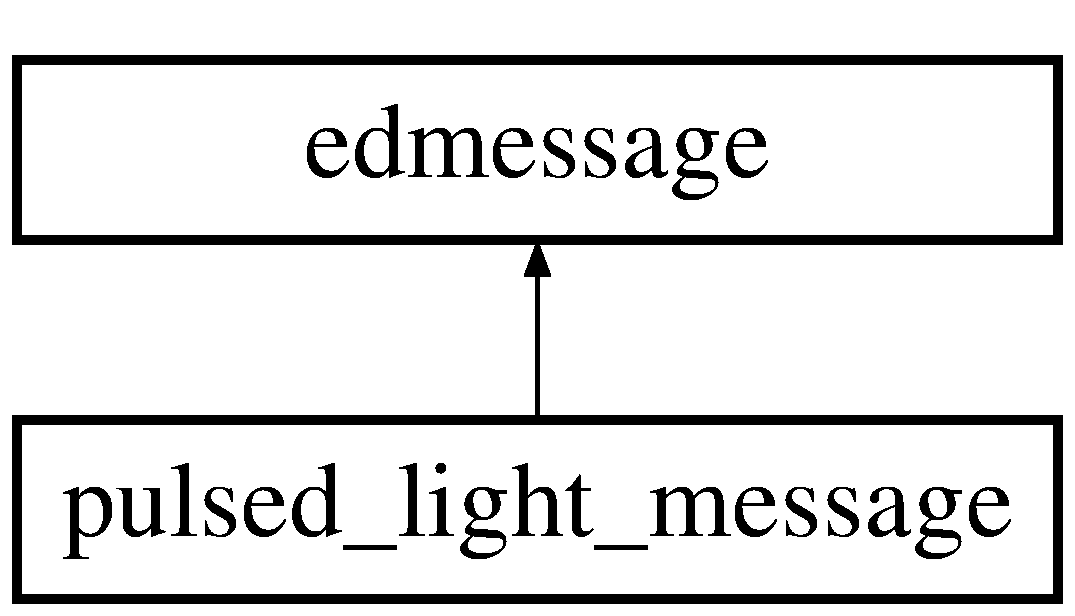
\includegraphics[height=2.000000cm]{structpulsed__light__message}
\end{center}
\end{figure}
\subsection*{Public Member Functions}
\begin{DoxyCompactItemize}
\item 
uint32\-\_\-t \hyperlink{structpulsed__light__message_a7202312fb93e2deb22bee2a84ac7a78d}{size} ()
\item 
std\-::string \hyperlink{structpulsed__light__message_af69b69dbd86e8fb7dc30ee3a304a5e35}{type} ()
\end{DoxyCompactItemize}
\subsection*{Static Public Member Functions}
\begin{DoxyCompactItemize}
\item 
static std\-::string \hyperlink{structpulsed__light__message_a3be8eb082c93bb7e957eb840436830da}{Type} ()
\end{DoxyCompactItemize}
\subsection*{Public Attributes}
\begin{DoxyCompactItemize}
\item 
\begin{tabbing}
xx\=xx\=xx\=xx\=xx\=xx\=xx\=xx\=xx\=\kill
union \{\\
\>struct \{\\
\>\>double \hyperlink{structpulsed__light__message_a978465139ddc4eaef1cf0bf5c87aa095}{distance1}\\
\>\>double \hyperlink{structpulsed__light__message_a5b2b73eea673eb1ba7c7793bb90d89d6}{distance2}\\
\>\>uint32\_t \hyperlink{structpulsed__light__message_aed1414064822ca15f33ab72b64b98a7d}{mraa\_pin1}\\
\>\>uint32\_t \hyperlink{structpulsed__light__message_aa36ddffc56849ff69e4cc17084f9635d}{mraa\_pin2}\\
\>\>double \hyperlink{structpulsed__light__message_ade8c428c9e6d99625033f3b0d74f96ad}{pos1} \mbox{[}3\mbox{]}\\
\>\>double \hyperlink{structpulsed__light__message_a598e2ddd86da341b3703b9a1e6a81d27}{pos2} \mbox{[}3\mbox{]}\\
\>\>double \hyperlink{structpulsed__light__message_aa50c043648567a006240ad6c39766898}{orientation1} \mbox{[}4\mbox{]}\\
\>\>double \hyperlink{structpulsed__light__message_a26ad20b42bc70bdf6299b4f69c8f3c91}{orientation2} \mbox{[}4\mbox{]}\\
\>\} \\
\>uint8\_t \hyperlink{structpulsed__light__message_a4598eab79d2487a7bdb3d1aa64a10e6f}{data} \mbox{[}136\mbox{]}\\
\}; \\

\end{tabbing}\end{DoxyCompactItemize}


\subsection{Member Function Documentation}
\hypertarget{structpulsed__light__message_a7202312fb93e2deb22bee2a84ac7a78d}{\index{pulsed\-\_\-light\-\_\-message@{pulsed\-\_\-light\-\_\-message}!size@{size}}
\index{size@{size}!pulsed_light_message@{pulsed\-\_\-light\-\_\-message}}
\subsubsection[{size}]{\setlength{\rightskip}{0pt plus 5cm}uint32\-\_\-t pulsed\-\_\-light\-\_\-message\-::size (
\begin{DoxyParamCaption}
{}
\end{DoxyParamCaption}
)\hspace{0.3cm}{\ttfamily [inline]}}}\label{structpulsed__light__message_a7202312fb93e2deb22bee2a84ac7a78d}
\hypertarget{structpulsed__light__message_af69b69dbd86e8fb7dc30ee3a304a5e35}{\index{pulsed\-\_\-light\-\_\-message@{pulsed\-\_\-light\-\_\-message}!type@{type}}
\index{type@{type}!pulsed_light_message@{pulsed\-\_\-light\-\_\-message}}
\subsubsection[{type}]{\setlength{\rightskip}{0pt plus 5cm}std\-::string pulsed\-\_\-light\-\_\-message\-::type (
\begin{DoxyParamCaption}
{}
\end{DoxyParamCaption}
)\hspace{0.3cm}{\ttfamily [inline]}, {\ttfamily [virtual]}}}\label{structpulsed__light__message_af69b69dbd86e8fb7dc30ee3a304a5e35}


Implements \hyperlink{structedmessage_ac888cf8e570a4aa9bea30a4c4fcdcc30}{edmessage}.

\hypertarget{structpulsed__light__message_a3be8eb082c93bb7e957eb840436830da}{\index{pulsed\-\_\-light\-\_\-message@{pulsed\-\_\-light\-\_\-message}!Type@{Type}}
\index{Type@{Type}!pulsed_light_message@{pulsed\-\_\-light\-\_\-message}}
\subsubsection[{Type}]{\setlength{\rightskip}{0pt plus 5cm}static std\-::string pulsed\-\_\-light\-\_\-message\-::\-Type (
\begin{DoxyParamCaption}
{}
\end{DoxyParamCaption}
)\hspace{0.3cm}{\ttfamily [inline]}, {\ttfamily [static]}}}\label{structpulsed__light__message_a3be8eb082c93bb7e957eb840436830da}


\subsection{Member Data Documentation}
\hypertarget{structpulsed__light__message_a61949b92c22465fb5342a702d320b357}{\subsubsection[{"@5}]{\setlength{\rightskip}{0pt plus 5cm}union \{ ... \} }}\label{structpulsed__light__message_a61949b92c22465fb5342a702d320b357}
\hypertarget{structpulsed__light__message_a4598eab79d2487a7bdb3d1aa64a10e6f}{\index{pulsed\-\_\-light\-\_\-message@{pulsed\-\_\-light\-\_\-message}!data@{data}}
\index{data@{data}!pulsed_light_message@{pulsed\-\_\-light\-\_\-message}}
\subsubsection[{data}]{\setlength{\rightskip}{0pt plus 5cm}uint8\-\_\-t pulsed\-\_\-light\-\_\-message\-::data\mbox{[}136\mbox{]}}}\label{structpulsed__light__message_a4598eab79d2487a7bdb3d1aa64a10e6f}
\hypertarget{structpulsed__light__message_a978465139ddc4eaef1cf0bf5c87aa095}{\index{pulsed\-\_\-light\-\_\-message@{pulsed\-\_\-light\-\_\-message}!distance1@{distance1}}
\index{distance1@{distance1}!pulsed_light_message@{pulsed\-\_\-light\-\_\-message}}
\subsubsection[{distance1}]{\setlength{\rightskip}{0pt plus 5cm}double pulsed\-\_\-light\-\_\-message\-::distance1}}\label{structpulsed__light__message_a978465139ddc4eaef1cf0bf5c87aa095}
\hypertarget{structpulsed__light__message_a5b2b73eea673eb1ba7c7793bb90d89d6}{\index{pulsed\-\_\-light\-\_\-message@{pulsed\-\_\-light\-\_\-message}!distance2@{distance2}}
\index{distance2@{distance2}!pulsed_light_message@{pulsed\-\_\-light\-\_\-message}}
\subsubsection[{distance2}]{\setlength{\rightskip}{0pt plus 5cm}double pulsed\-\_\-light\-\_\-message\-::distance2}}\label{structpulsed__light__message_a5b2b73eea673eb1ba7c7793bb90d89d6}
\hypertarget{structpulsed__light__message_aed1414064822ca15f33ab72b64b98a7d}{\index{pulsed\-\_\-light\-\_\-message@{pulsed\-\_\-light\-\_\-message}!mraa\-\_\-pin1@{mraa\-\_\-pin1}}
\index{mraa\-\_\-pin1@{mraa\-\_\-pin1}!pulsed_light_message@{pulsed\-\_\-light\-\_\-message}}
\subsubsection[{mraa\-\_\-pin1}]{\setlength{\rightskip}{0pt plus 5cm}uint32\-\_\-t pulsed\-\_\-light\-\_\-message\-::mraa\-\_\-pin1}}\label{structpulsed__light__message_aed1414064822ca15f33ab72b64b98a7d}
\hypertarget{structpulsed__light__message_aa36ddffc56849ff69e4cc17084f9635d}{\index{pulsed\-\_\-light\-\_\-message@{pulsed\-\_\-light\-\_\-message}!mraa\-\_\-pin2@{mraa\-\_\-pin2}}
\index{mraa\-\_\-pin2@{mraa\-\_\-pin2}!pulsed_light_message@{pulsed\-\_\-light\-\_\-message}}
\subsubsection[{mraa\-\_\-pin2}]{\setlength{\rightskip}{0pt plus 5cm}uint32\-\_\-t pulsed\-\_\-light\-\_\-message\-::mraa\-\_\-pin2}}\label{structpulsed__light__message_aa36ddffc56849ff69e4cc17084f9635d}
\hypertarget{structpulsed__light__message_aa50c043648567a006240ad6c39766898}{\index{pulsed\-\_\-light\-\_\-message@{pulsed\-\_\-light\-\_\-message}!orientation1@{orientation1}}
\index{orientation1@{orientation1}!pulsed_light_message@{pulsed\-\_\-light\-\_\-message}}
\subsubsection[{orientation1}]{\setlength{\rightskip}{0pt plus 5cm}double pulsed\-\_\-light\-\_\-message\-::orientation1\mbox{[}4\mbox{]}}}\label{structpulsed__light__message_aa50c043648567a006240ad6c39766898}
\hypertarget{structpulsed__light__message_a26ad20b42bc70bdf6299b4f69c8f3c91}{\index{pulsed\-\_\-light\-\_\-message@{pulsed\-\_\-light\-\_\-message}!orientation2@{orientation2}}
\index{orientation2@{orientation2}!pulsed_light_message@{pulsed\-\_\-light\-\_\-message}}
\subsubsection[{orientation2}]{\setlength{\rightskip}{0pt plus 5cm}double pulsed\-\_\-light\-\_\-message\-::orientation2\mbox{[}4\mbox{]}}}\label{structpulsed__light__message_a26ad20b42bc70bdf6299b4f69c8f3c91}
\hypertarget{structpulsed__light__message_ade8c428c9e6d99625033f3b0d74f96ad}{\index{pulsed\-\_\-light\-\_\-message@{pulsed\-\_\-light\-\_\-message}!pos1@{pos1}}
\index{pos1@{pos1}!pulsed_light_message@{pulsed\-\_\-light\-\_\-message}}
\subsubsection[{pos1}]{\setlength{\rightskip}{0pt plus 5cm}double pulsed\-\_\-light\-\_\-message\-::pos1\mbox{[}3\mbox{]}}}\label{structpulsed__light__message_ade8c428c9e6d99625033f3b0d74f96ad}
\hypertarget{structpulsed__light__message_a598e2ddd86da341b3703b9a1e6a81d27}{\index{pulsed\-\_\-light\-\_\-message@{pulsed\-\_\-light\-\_\-message}!pos2@{pos2}}
\index{pos2@{pos2}!pulsed_light_message@{pulsed\-\_\-light\-\_\-message}}
\subsubsection[{pos2}]{\setlength{\rightskip}{0pt plus 5cm}double pulsed\-\_\-light\-\_\-message\-::pos2\mbox{[}3\mbox{]}}}\label{structpulsed__light__message_a598e2ddd86da341b3703b9a1e6a81d27}


The documentation for this struct was generated from the following file\-:\begin{DoxyCompactItemize}
\item 
/home/dprandle/\-Documents/code/ctrlmod/include/\hyperlink{edmessage_8h}{edmessage.\-h}\end{DoxyCompactItemize}

\hypertarget{structrequest__packet}{\section{request\-\_\-packet Struct Reference}
\label{structrequest__packet}\index{request\-\_\-packet@{request\-\_\-packet}}
}


{\ttfamily \#include $<$edrplidar\-\_\-packets.\-h$>$}

Inheritance diagram for request\-\_\-packet\-:\begin{figure}[H]
\begin{center}
\leavevmode
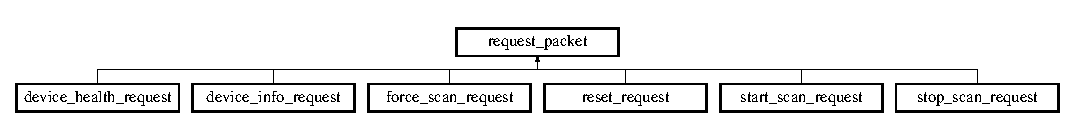
\includegraphics[height=1.269841cm]{structrequest__packet}
\end{center}
\end{figure}
\subsection*{Public Member Functions}
\begin{DoxyCompactItemize}
\item 
\hyperlink{structrequest__packet_a0c8aac3f578beedf0546ca9ad7bdcf6b}{request\-\_\-packet} (uint8\-\_\-t M\-S\-B, uint8\-\_\-t L\-S\-B)
\item 
virtual \hyperlink{structrequest__packet_a8807bb7660042e8b5d024e0b494d5165}{$\sim$request\-\_\-packet} ()
\end{DoxyCompactItemize}
\subsection*{Public Attributes}
\begin{DoxyCompactItemize}
\item 
\begin{tabbing}
xx\=xx\=xx\=xx\=xx\=xx\=xx\=xx\=xx\=\kill
union \{\\
\>struct \{\\
\>\>uint8\_t \hyperlink{structrequest__packet_a5b313981d2e1b5d5966b0e76df27f2a1}{msB}\\
\>\>uint8\_t \hyperlink{structrequest__packet_a8acbd68bdbd185926f3a4addb920488b}{lsB}\\
\>\} \\
\>uint8\_t \hyperlink{structrequest__packet_aa491a1d59ef4c4b2d40575569e9c5e2d}{data} \mbox{[}2\mbox{]}\\
\}; \\

\end{tabbing}\end{DoxyCompactItemize}


\subsection{Constructor \& Destructor Documentation}
\hypertarget{structrequest__packet_a0c8aac3f578beedf0546ca9ad7bdcf6b}{\index{request\-\_\-packet@{request\-\_\-packet}!request\-\_\-packet@{request\-\_\-packet}}
\index{request\-\_\-packet@{request\-\_\-packet}!request_packet@{request\-\_\-packet}}
\subsubsection[{request\-\_\-packet}]{\setlength{\rightskip}{0pt plus 5cm}request\-\_\-packet\-::request\-\_\-packet (
\begin{DoxyParamCaption}
\item[{uint8\-\_\-t}]{M\-S\-B, }
\item[{uint8\-\_\-t}]{L\-S\-B}
\end{DoxyParamCaption}
)\hspace{0.3cm}{\ttfamily [inline]}}}\label{structrequest__packet_a0c8aac3f578beedf0546ca9ad7bdcf6b}
\hypertarget{structrequest__packet_a8807bb7660042e8b5d024e0b494d5165}{\index{request\-\_\-packet@{request\-\_\-packet}!$\sim$request\-\_\-packet@{$\sim$request\-\_\-packet}}
\index{$\sim$request\-\_\-packet@{$\sim$request\-\_\-packet}!request_packet@{request\-\_\-packet}}
\subsubsection[{$\sim$request\-\_\-packet}]{\setlength{\rightskip}{0pt plus 5cm}virtual request\-\_\-packet\-::$\sim$request\-\_\-packet (
\begin{DoxyParamCaption}
{}
\end{DoxyParamCaption}
)\hspace{0.3cm}{\ttfamily [inline]}, {\ttfamily [virtual]}}}\label{structrequest__packet_a8807bb7660042e8b5d024e0b494d5165}


\subsection{Member Data Documentation}
\hypertarget{structrequest__packet_a7f612f9825a53cf4f1440eb566a1bff2}{\subsubsection[{"@29}]{\setlength{\rightskip}{0pt plus 5cm}union \{ ... \} }}\label{structrequest__packet_a7f612f9825a53cf4f1440eb566a1bff2}
\hypertarget{structrequest__packet_aa491a1d59ef4c4b2d40575569e9c5e2d}{\index{request\-\_\-packet@{request\-\_\-packet}!data@{data}}
\index{data@{data}!request_packet@{request\-\_\-packet}}
\subsubsection[{data}]{\setlength{\rightskip}{0pt plus 5cm}uint8\-\_\-t request\-\_\-packet\-::data\mbox{[}2\mbox{]}}}\label{structrequest__packet_aa491a1d59ef4c4b2d40575569e9c5e2d}
\hypertarget{structrequest__packet_a8acbd68bdbd185926f3a4addb920488b}{\index{request\-\_\-packet@{request\-\_\-packet}!ls\-B@{ls\-B}}
\index{ls\-B@{ls\-B}!request_packet@{request\-\_\-packet}}
\subsubsection[{ls\-B}]{\setlength{\rightskip}{0pt plus 5cm}uint8\-\_\-t request\-\_\-packet\-::ls\-B}}\label{structrequest__packet_a8acbd68bdbd185926f3a4addb920488b}
\hypertarget{structrequest__packet_a5b313981d2e1b5d5966b0e76df27f2a1}{\index{request\-\_\-packet@{request\-\_\-packet}!ms\-B@{ms\-B}}
\index{ms\-B@{ms\-B}!request_packet@{request\-\_\-packet}}
\subsubsection[{ms\-B}]{\setlength{\rightskip}{0pt plus 5cm}uint8\-\_\-t request\-\_\-packet\-::ms\-B}}\label{structrequest__packet_a5b313981d2e1b5d5966b0e76df27f2a1}


The documentation for this struct was generated from the following file\-:\begin{DoxyCompactItemize}
\item 
/home/dprandle/\-Documents/code/ctrlmod/include/\hyperlink{edrplidar__packets_8h}{edrplidar\-\_\-packets.\-h}\end{DoxyCompactItemize}

\hypertarget{structreset__request}{\section{reset\-\_\-request Struct Reference}
\label{structreset__request}\index{reset\-\_\-request@{reset\-\_\-request}}
}


{\ttfamily \#include $<$edrplidar\-\_\-packets.\-h$>$}

Inheritance diagram for reset\-\_\-request\-:\begin{figure}[H]
\begin{center}
\leavevmode
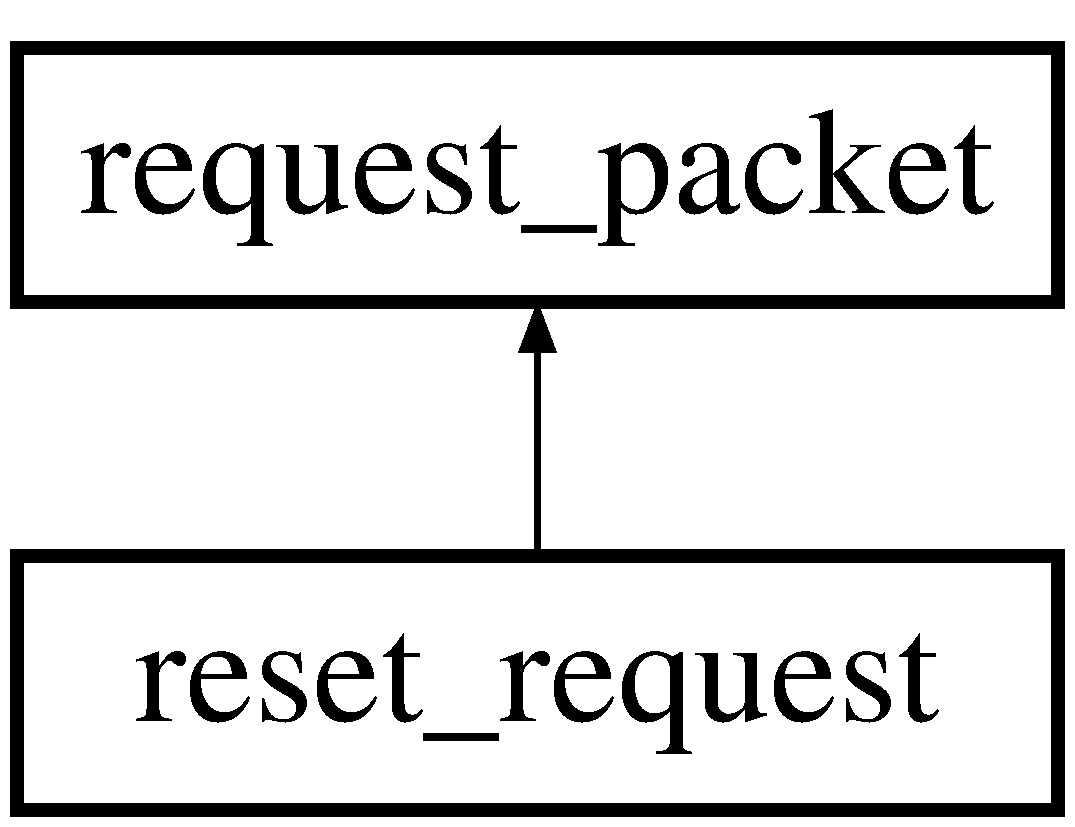
\includegraphics[height=2.000000cm]{structreset__request}
\end{center}
\end{figure}
\subsection*{Public Member Functions}
\begin{DoxyCompactItemize}
\item 
\hyperlink{structreset__request_a41d5cf503ff5f1ea7c260c0cd160b253}{reset\-\_\-request} ()
\end{DoxyCompactItemize}
\subsection*{Additional Inherited Members}


\subsection{Constructor \& Destructor Documentation}
\hypertarget{structreset__request_a41d5cf503ff5f1ea7c260c0cd160b253}{\index{reset\-\_\-request@{reset\-\_\-request}!reset\-\_\-request@{reset\-\_\-request}}
\index{reset\-\_\-request@{reset\-\_\-request}!reset_request@{reset\-\_\-request}}
\subsubsection[{reset\-\_\-request}]{\setlength{\rightskip}{0pt plus 5cm}reset\-\_\-request\-::reset\-\_\-request (
\begin{DoxyParamCaption}
{}
\end{DoxyParamCaption}
)\hspace{0.3cm}{\ttfamily [inline]}}}\label{structreset__request_a41d5cf503ff5f1ea7c260c0cd160b253}


The documentation for this struct was generated from the following file\-:\begin{DoxyCompactItemize}
\item 
/home/dprandle/\-Documents/code/ctrlmod/include/\hyperlink{edrplidar__packets_8h}{edrplidar\-\_\-packets.\-h}\end{DoxyCompactItemize}

\hypertarget{structrplidar__error__message}{\section{rplidar\-\_\-error\-\_\-message Struct Reference}
\label{structrplidar__error__message}\index{rplidar\-\_\-error\-\_\-message@{rplidar\-\_\-error\-\_\-message}}
}


{\ttfamily \#include $<$edmessage.\-h$>$}

Inheritance diagram for rplidar\-\_\-error\-\_\-message\-:\begin{figure}[H]
\begin{center}
\leavevmode
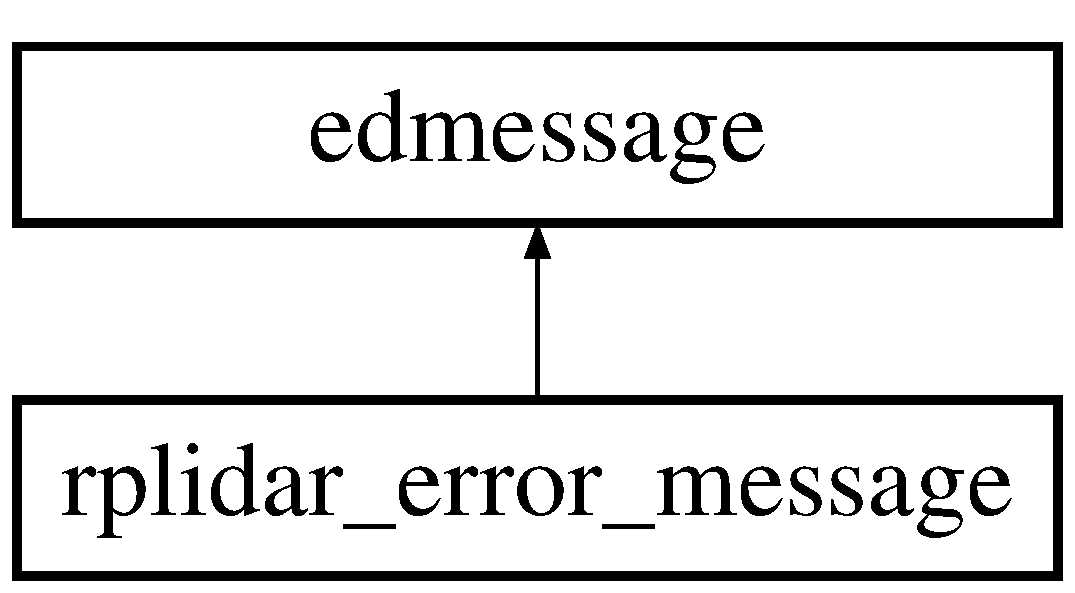
\includegraphics[height=2.000000cm]{structrplidar__error__message}
\end{center}
\end{figure}
\subsection*{Public Member Functions}
\begin{DoxyCompactItemize}
\item 
\hyperlink{structrplidar__error__message_af4f1902c3778e4289eac7a4ab20cdc12}{rplidar\-\_\-error\-\_\-message} ()
\item 
virtual std\-::string \hyperlink{structrplidar__error__message_a3041dd23bfc9e0b5612bd7ce75849ea1}{type} ()
\end{DoxyCompactItemize}
\subsection*{Static Public Member Functions}
\begin{DoxyCompactItemize}
\item 
static std\-::string \hyperlink{structrplidar__error__message_aca98493f4795168785997efbb1008fae}{Type} ()
\end{DoxyCompactItemize}
\subsection*{Public Attributes}
\begin{DoxyCompactItemize}
\item 
uint8\-\_\-t \hyperlink{structrplidar__error__message_a788f75a0c9edbe2c0c154dbe3b48672f}{message} \mbox{[}100\mbox{]}
\end{DoxyCompactItemize}


\subsection{Constructor \& Destructor Documentation}
\hypertarget{structrplidar__error__message_af4f1902c3778e4289eac7a4ab20cdc12}{\index{rplidar\-\_\-error\-\_\-message@{rplidar\-\_\-error\-\_\-message}!rplidar\-\_\-error\-\_\-message@{rplidar\-\_\-error\-\_\-message}}
\index{rplidar\-\_\-error\-\_\-message@{rplidar\-\_\-error\-\_\-message}!rplidar_error_message@{rplidar\-\_\-error\-\_\-message}}
\subsubsection[{rplidar\-\_\-error\-\_\-message}]{\setlength{\rightskip}{0pt plus 5cm}rplidar\-\_\-error\-\_\-message\-::rplidar\-\_\-error\-\_\-message (
\begin{DoxyParamCaption}
{}
\end{DoxyParamCaption}
)}}\label{structrplidar__error__message_af4f1902c3778e4289eac7a4ab20cdc12}


\subsection{Member Function Documentation}
\hypertarget{structrplidar__error__message_a3041dd23bfc9e0b5612bd7ce75849ea1}{\index{rplidar\-\_\-error\-\_\-message@{rplidar\-\_\-error\-\_\-message}!type@{type}}
\index{type@{type}!rplidar_error_message@{rplidar\-\_\-error\-\_\-message}}
\subsubsection[{type}]{\setlength{\rightskip}{0pt plus 5cm}virtual std\-::string rplidar\-\_\-error\-\_\-message\-::type (
\begin{DoxyParamCaption}
{}
\end{DoxyParamCaption}
)\hspace{0.3cm}{\ttfamily [inline]}, {\ttfamily [virtual]}}}\label{structrplidar__error__message_a3041dd23bfc9e0b5612bd7ce75849ea1}


Implements \hyperlink{structedmessage_ac888cf8e570a4aa9bea30a4c4fcdcc30}{edmessage}.

\hypertarget{structrplidar__error__message_aca98493f4795168785997efbb1008fae}{\index{rplidar\-\_\-error\-\_\-message@{rplidar\-\_\-error\-\_\-message}!Type@{Type}}
\index{Type@{Type}!rplidar_error_message@{rplidar\-\_\-error\-\_\-message}}
\subsubsection[{Type}]{\setlength{\rightskip}{0pt plus 5cm}static std\-::string rplidar\-\_\-error\-\_\-message\-::\-Type (
\begin{DoxyParamCaption}
{}
\end{DoxyParamCaption}
)\hspace{0.3cm}{\ttfamily [inline]}, {\ttfamily [static]}}}\label{structrplidar__error__message_aca98493f4795168785997efbb1008fae}


\subsection{Member Data Documentation}
\hypertarget{structrplidar__error__message_a788f75a0c9edbe2c0c154dbe3b48672f}{\index{rplidar\-\_\-error\-\_\-message@{rplidar\-\_\-error\-\_\-message}!message@{message}}
\index{message@{message}!rplidar_error_message@{rplidar\-\_\-error\-\_\-message}}
\subsubsection[{message}]{\setlength{\rightskip}{0pt plus 5cm}uint8\-\_\-t rplidar\-\_\-error\-\_\-message\-::message\mbox{[}100\mbox{]}}}\label{structrplidar__error__message_a788f75a0c9edbe2c0c154dbe3b48672f}


The documentation for this struct was generated from the following files\-:\begin{DoxyCompactItemize}
\item 
/home/dprandle/\-Documents/code/ctrlmod/include/\hyperlink{edmessage_8h}{edmessage.\-h}\item 
/home/dprandle/\-Documents/code/ctrlmod/src/\hyperlink{edmessage_8cpp}{edmessage.\-cpp}\end{DoxyCompactItemize}

\hypertarget{structrplidar__firmware__message}{\section{rplidar\-\_\-firmware\-\_\-message Struct Reference}
\label{structrplidar__firmware__message}\index{rplidar\-\_\-firmware\-\_\-message@{rplidar\-\_\-firmware\-\_\-message}}
}


{\ttfamily \#include $<$edmessage.\-h$>$}

Inheritance diagram for rplidar\-\_\-firmware\-\_\-message\-:\begin{figure}[H]
\begin{center}
\leavevmode
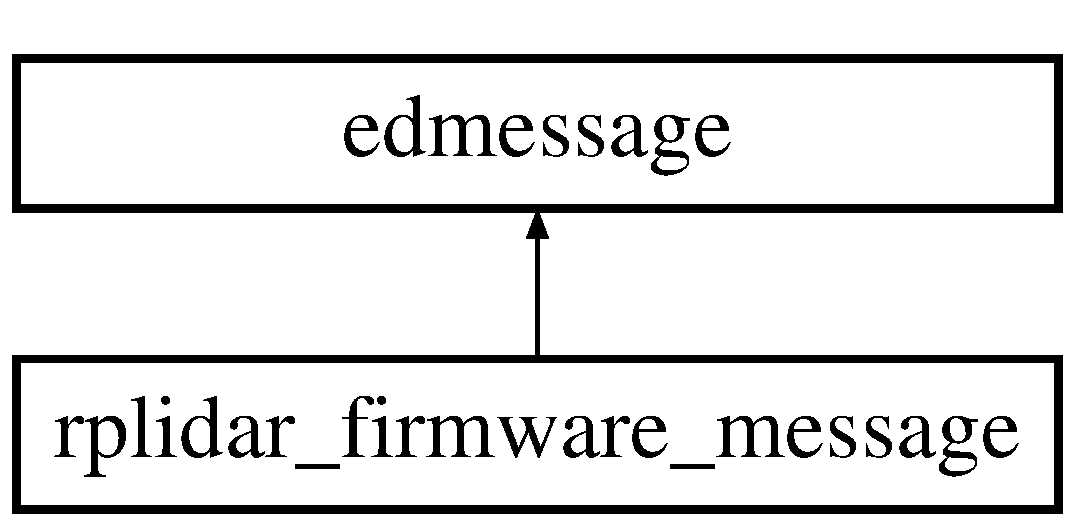
\includegraphics[height=2.000000cm]{structrplidar__firmware__message}
\end{center}
\end{figure}
\subsection*{Public Member Functions}
\begin{DoxyCompactItemize}
\item 
virtual std\-::string \hyperlink{structrplidar__firmware__message_a6985ec56070c19af62cf4b95dbeb78f8}{type} ()
\end{DoxyCompactItemize}
\subsection*{Static Public Member Functions}
\begin{DoxyCompactItemize}
\item 
static std\-::string \hyperlink{structrplidar__firmware__message_a2ef1ac448780fdccaee555703b82d83e}{Type} ()
\end{DoxyCompactItemize}
\subsection*{Public Attributes}
\begin{DoxyCompactItemize}
\item 
\hyperlink{structfirmware__data__packet}{firmware\-\_\-data\-\_\-packet} \hyperlink{structrplidar__firmware__message_a0bed4488959ae399d04e8939dcc8bbcd}{device\-\_\-firmware}
\end{DoxyCompactItemize}


\subsection{Member Function Documentation}
\hypertarget{structrplidar__firmware__message_a6985ec56070c19af62cf4b95dbeb78f8}{\index{rplidar\-\_\-firmware\-\_\-message@{rplidar\-\_\-firmware\-\_\-message}!type@{type}}
\index{type@{type}!rplidar_firmware_message@{rplidar\-\_\-firmware\-\_\-message}}
\subsubsection[{type}]{\setlength{\rightskip}{0pt plus 5cm}virtual std\-::string rplidar\-\_\-firmware\-\_\-message\-::type (
\begin{DoxyParamCaption}
{}
\end{DoxyParamCaption}
)\hspace{0.3cm}{\ttfamily [inline]}, {\ttfamily [virtual]}}}\label{structrplidar__firmware__message_a6985ec56070c19af62cf4b95dbeb78f8}


Implements \hyperlink{structedmessage_ac888cf8e570a4aa9bea30a4c4fcdcc30}{edmessage}.

\hypertarget{structrplidar__firmware__message_a2ef1ac448780fdccaee555703b82d83e}{\index{rplidar\-\_\-firmware\-\_\-message@{rplidar\-\_\-firmware\-\_\-message}!Type@{Type}}
\index{Type@{Type}!rplidar_firmware_message@{rplidar\-\_\-firmware\-\_\-message}}
\subsubsection[{Type}]{\setlength{\rightskip}{0pt plus 5cm}static std\-::string rplidar\-\_\-firmware\-\_\-message\-::\-Type (
\begin{DoxyParamCaption}
{}
\end{DoxyParamCaption}
)\hspace{0.3cm}{\ttfamily [inline]}, {\ttfamily [static]}}}\label{structrplidar__firmware__message_a2ef1ac448780fdccaee555703b82d83e}


\subsection{Member Data Documentation}
\hypertarget{structrplidar__firmware__message_a0bed4488959ae399d04e8939dcc8bbcd}{\index{rplidar\-\_\-firmware\-\_\-message@{rplidar\-\_\-firmware\-\_\-message}!device\-\_\-firmware@{device\-\_\-firmware}}
\index{device\-\_\-firmware@{device\-\_\-firmware}!rplidar_firmware_message@{rplidar\-\_\-firmware\-\_\-message}}
\subsubsection[{device\-\_\-firmware}]{\setlength{\rightskip}{0pt plus 5cm}{\bf firmware\-\_\-data\-\_\-packet} rplidar\-\_\-firmware\-\_\-message\-::device\-\_\-firmware}}\label{structrplidar__firmware__message_a0bed4488959ae399d04e8939dcc8bbcd}


The documentation for this struct was generated from the following file\-:\begin{DoxyCompactItemize}
\item 
/home/dprandle/\-Documents/code/ctrlmod/include/\hyperlink{edmessage_8h}{edmessage.\-h}\end{DoxyCompactItemize}

\hypertarget{structrplidar__health__message}{\section{rplidar\-\_\-health\-\_\-message Struct Reference}
\label{structrplidar__health__message}\index{rplidar\-\_\-health\-\_\-message@{rplidar\-\_\-health\-\_\-message}}
}


{\ttfamily \#include $<$edmessage.\-h$>$}

Inheritance diagram for rplidar\-\_\-health\-\_\-message\-:\begin{figure}[H]
\begin{center}
\leavevmode
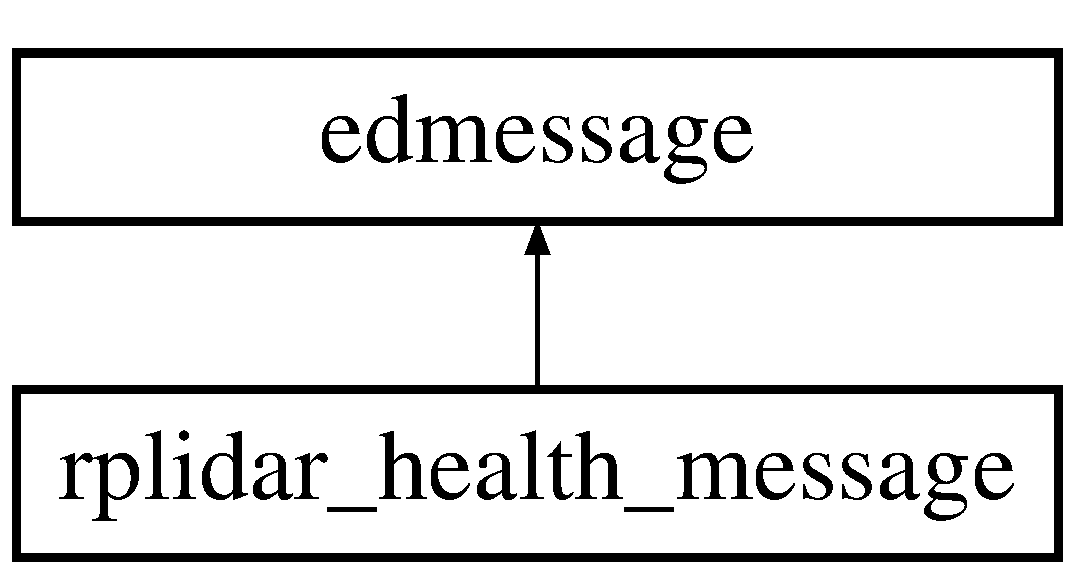
\includegraphics[height=2.000000cm]{structrplidar__health__message}
\end{center}
\end{figure}
\subsection*{Public Member Functions}
\begin{DoxyCompactItemize}
\item 
virtual std\-::string \hyperlink{structrplidar__health__message_aa886bee47423f541669914e883b838ee}{type} ()
\end{DoxyCompactItemize}
\subsection*{Static Public Member Functions}
\begin{DoxyCompactItemize}
\item 
static std\-::string \hyperlink{structrplidar__health__message_ac69cee0b7a99e25d03b67ad7eecd8b49}{Type} ()
\end{DoxyCompactItemize}
\subsection*{Public Attributes}
\begin{DoxyCompactItemize}
\item 
\hyperlink{structhealth__data__packet}{health\-\_\-data\-\_\-packet} \hyperlink{structrplidar__health__message_a5e2fa670530fc053c45278d04c681bd2}{device\-\_\-health}
\end{DoxyCompactItemize}


\subsection{Member Function Documentation}
\hypertarget{structrplidar__health__message_aa886bee47423f541669914e883b838ee}{\index{rplidar\-\_\-health\-\_\-message@{rplidar\-\_\-health\-\_\-message}!type@{type}}
\index{type@{type}!rplidar_health_message@{rplidar\-\_\-health\-\_\-message}}
\subsubsection[{type}]{\setlength{\rightskip}{0pt plus 5cm}virtual std\-::string rplidar\-\_\-health\-\_\-message\-::type (
\begin{DoxyParamCaption}
{}
\end{DoxyParamCaption}
)\hspace{0.3cm}{\ttfamily [inline]}, {\ttfamily [virtual]}}}\label{structrplidar__health__message_aa886bee47423f541669914e883b838ee}


Implements \hyperlink{structedmessage_ac888cf8e570a4aa9bea30a4c4fcdcc30}{edmessage}.

\hypertarget{structrplidar__health__message_ac69cee0b7a99e25d03b67ad7eecd8b49}{\index{rplidar\-\_\-health\-\_\-message@{rplidar\-\_\-health\-\_\-message}!Type@{Type}}
\index{Type@{Type}!rplidar_health_message@{rplidar\-\_\-health\-\_\-message}}
\subsubsection[{Type}]{\setlength{\rightskip}{0pt plus 5cm}static std\-::string rplidar\-\_\-health\-\_\-message\-::\-Type (
\begin{DoxyParamCaption}
{}
\end{DoxyParamCaption}
)\hspace{0.3cm}{\ttfamily [inline]}, {\ttfamily [static]}}}\label{structrplidar__health__message_ac69cee0b7a99e25d03b67ad7eecd8b49}


\subsection{Member Data Documentation}
\hypertarget{structrplidar__health__message_a5e2fa670530fc053c45278d04c681bd2}{\index{rplidar\-\_\-health\-\_\-message@{rplidar\-\_\-health\-\_\-message}!device\-\_\-health@{device\-\_\-health}}
\index{device\-\_\-health@{device\-\_\-health}!rplidar_health_message@{rplidar\-\_\-health\-\_\-message}}
\subsubsection[{device\-\_\-health}]{\setlength{\rightskip}{0pt plus 5cm}{\bf health\-\_\-data\-\_\-packet} rplidar\-\_\-health\-\_\-message\-::device\-\_\-health}}\label{structrplidar__health__message_a5e2fa670530fc053c45278d04c681bd2}


The documentation for this struct was generated from the following file\-:\begin{DoxyCompactItemize}
\item 
/home/dprandle/\-Documents/code/ctrlmod/include/\hyperlink{edmessage_8h}{edmessage.\-h}\end{DoxyCompactItemize}

\hypertarget{structrplidar__info__message}{\section{rplidar\-\_\-info\-\_\-message Struct Reference}
\label{structrplidar__info__message}\index{rplidar\-\_\-info\-\_\-message@{rplidar\-\_\-info\-\_\-message}}
}


{\ttfamily \#include $<$edmessage.\-h$>$}

Inheritance diagram for rplidar\-\_\-info\-\_\-message\-:\begin{figure}[H]
\begin{center}
\leavevmode
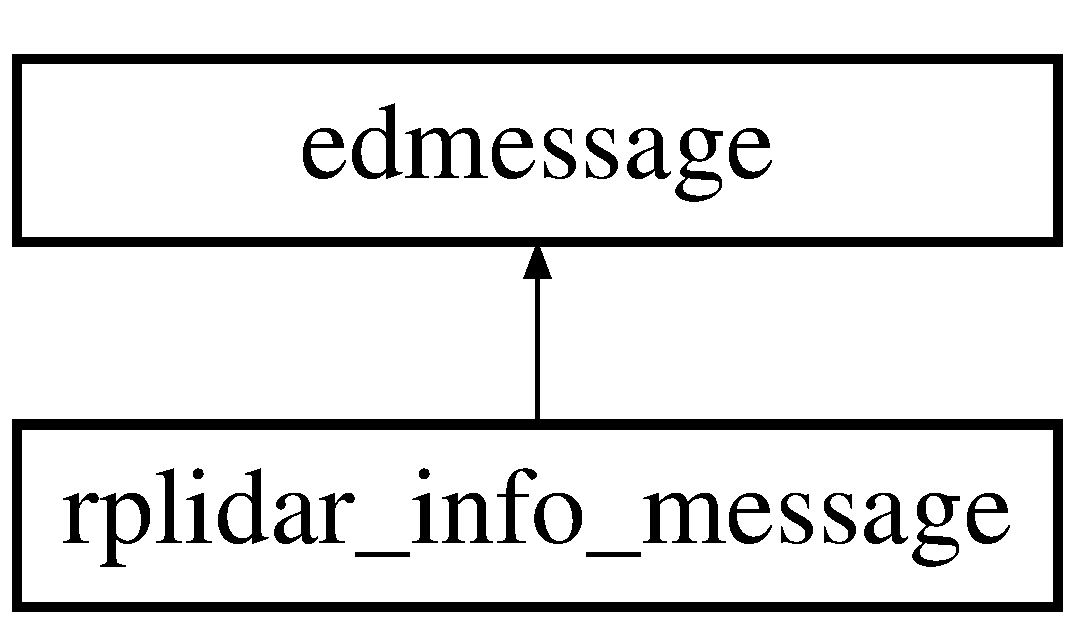
\includegraphics[height=2.000000cm]{structrplidar__info__message}
\end{center}
\end{figure}
\subsection*{Public Member Functions}
\begin{DoxyCompactItemize}
\item 
virtual std\-::string \hyperlink{structrplidar__info__message_a05bacd569c40d9f88ef4374af34bea49}{type} ()
\end{DoxyCompactItemize}
\subsection*{Static Public Member Functions}
\begin{DoxyCompactItemize}
\item 
static std\-::string \hyperlink{structrplidar__info__message_a14754c933c3157601c2a006ecbf5cf62}{Type} ()
\end{DoxyCompactItemize}
\subsection*{Public Attributes}
\begin{DoxyCompactItemize}
\item 
\hyperlink{structinfo__data__packet}{info\-\_\-data\-\_\-packet} \hyperlink{structrplidar__info__message_a6bb845edccde9eb8568c018ae2070ced}{device\-\_\-info}
\end{DoxyCompactItemize}


\subsection{Member Function Documentation}
\hypertarget{structrplidar__info__message_a05bacd569c40d9f88ef4374af34bea49}{\index{rplidar\-\_\-info\-\_\-message@{rplidar\-\_\-info\-\_\-message}!type@{type}}
\index{type@{type}!rplidar_info_message@{rplidar\-\_\-info\-\_\-message}}
\subsubsection[{type}]{\setlength{\rightskip}{0pt plus 5cm}virtual std\-::string rplidar\-\_\-info\-\_\-message\-::type (
\begin{DoxyParamCaption}
{}
\end{DoxyParamCaption}
)\hspace{0.3cm}{\ttfamily [inline]}, {\ttfamily [virtual]}}}\label{structrplidar__info__message_a05bacd569c40d9f88ef4374af34bea49}


Implements \hyperlink{structedmessage_ac888cf8e570a4aa9bea30a4c4fcdcc30}{edmessage}.

\hypertarget{structrplidar__info__message_a14754c933c3157601c2a006ecbf5cf62}{\index{rplidar\-\_\-info\-\_\-message@{rplidar\-\_\-info\-\_\-message}!Type@{Type}}
\index{Type@{Type}!rplidar_info_message@{rplidar\-\_\-info\-\_\-message}}
\subsubsection[{Type}]{\setlength{\rightskip}{0pt plus 5cm}static std\-::string rplidar\-\_\-info\-\_\-message\-::\-Type (
\begin{DoxyParamCaption}
{}
\end{DoxyParamCaption}
)\hspace{0.3cm}{\ttfamily [inline]}, {\ttfamily [static]}}}\label{structrplidar__info__message_a14754c933c3157601c2a006ecbf5cf62}


\subsection{Member Data Documentation}
\hypertarget{structrplidar__info__message_a6bb845edccde9eb8568c018ae2070ced}{\index{rplidar\-\_\-info\-\_\-message@{rplidar\-\_\-info\-\_\-message}!device\-\_\-info@{device\-\_\-info}}
\index{device\-\_\-info@{device\-\_\-info}!rplidar_info_message@{rplidar\-\_\-info\-\_\-message}}
\subsubsection[{device\-\_\-info}]{\setlength{\rightskip}{0pt plus 5cm}{\bf info\-\_\-data\-\_\-packet} rplidar\-\_\-info\-\_\-message\-::device\-\_\-info}}\label{structrplidar__info__message_a6bb845edccde9eb8568c018ae2070ced}


The documentation for this struct was generated from the following file\-:\begin{DoxyCompactItemize}
\item 
/home/dprandle/\-Documents/code/ctrlmod/include/\hyperlink{edmessage_8h}{edmessage.\-h}\end{DoxyCompactItemize}

\hypertarget{structrplidar__request}{\section{rplidar\-\_\-request Struct Reference}
\label{structrplidar__request}\index{rplidar\-\_\-request@{rplidar\-\_\-request}}
}


{\ttfamily \#include $<$edmessage.\-h$>$}

Inheritance diagram for rplidar\-\_\-request\-:\begin{figure}[H]
\begin{center}
\leavevmode
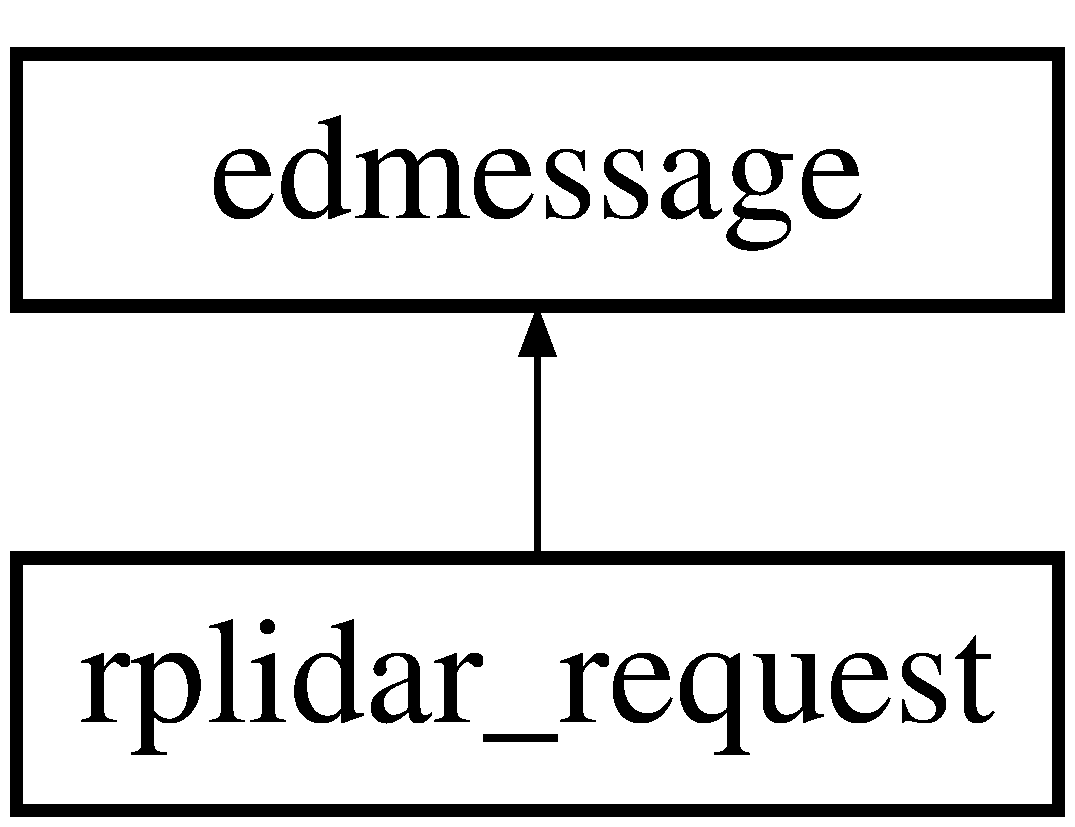
\includegraphics[height=2.000000cm]{structrplidar__request}
\end{center}
\end{figure}
\subsection*{Public Types}
\begin{DoxyCompactItemize}
\item 
enum \hyperlink{structrplidar__request_a7a2aceb50d6779e0d0ca188d18542c75}{req\-\_\-type} \{ \\*
\hyperlink{structrplidar__request_a7a2aceb50d6779e0d0ca188d18542c75aec752da288a10cb540712a9910785b3d}{Health\-Req}, 
\hyperlink{structrplidar__request_a7a2aceb50d6779e0d0ca188d18542c75abc412c174f6810a858521f3bd5f136c9}{Info\-Req}, 
\hyperlink{structrplidar__request_a7a2aceb50d6779e0d0ca188d18542c75a9d7bdb72d07a35486c428690f36d1922}{Start\-Scan}, 
\hyperlink{structrplidar__request_a7a2aceb50d6779e0d0ca188d18542c75a8ee556fc213c3b12c7f2f938e8eb9a45}{Force\-Scan}, 
\\*
\hyperlink{structrplidar__request_a7a2aceb50d6779e0d0ca188d18542c75a490bbda14afdffd8124e436f67897405}{Stop\-Scan}, 
\hyperlink{structrplidar__request_a7a2aceb50d6779e0d0ca188d18542c75a8bb842fd26be4238785e41946562c5ff}{Reset}
 \}
\end{DoxyCompactItemize}
\subsection*{Public Member Functions}
\begin{DoxyCompactItemize}
\item 
virtual std\-::string \hyperlink{structrplidar__request_af5765bf9fe3d05e9642a255f3b9edfdc}{type} ()
\end{DoxyCompactItemize}
\subsection*{Static Public Member Functions}
\begin{DoxyCompactItemize}
\item 
static std\-::string \hyperlink{structrplidar__request_a9b610deef1856be76f6a5b2a43275859}{Type} ()
\end{DoxyCompactItemize}
\subsection*{Public Attributes}
\begin{DoxyCompactItemize}
\item 
\hyperlink{structrplidar__request_a7a2aceb50d6779e0d0ca188d18542c75}{req\-\_\-type} \hyperlink{structrplidar__request_a11eebc40e0444f2a73765fbb08953fc4}{r\-\_\-type}
\end{DoxyCompactItemize}


\subsection{Member Enumeration Documentation}
\hypertarget{structrplidar__request_a7a2aceb50d6779e0d0ca188d18542c75}{\index{rplidar\-\_\-request@{rplidar\-\_\-request}!req\-\_\-type@{req\-\_\-type}}
\index{req\-\_\-type@{req\-\_\-type}!rplidar_request@{rplidar\-\_\-request}}
\subsubsection[{req\-\_\-type}]{\setlength{\rightskip}{0pt plus 5cm}enum {\bf rplidar\-\_\-request\-::req\-\_\-type}}}\label{structrplidar__request_a7a2aceb50d6779e0d0ca188d18542c75}
\begin{Desc}
\item[Enumerator]\par
\begin{description}
\index{Health\-Req@{Health\-Req}!rplidar\-\_\-request@{rplidar\-\_\-request}}\index{rplidar\-\_\-request@{rplidar\-\_\-request}!Health\-Req@{Health\-Req}}\item[{\em 
\hypertarget{structrplidar__request_a7a2aceb50d6779e0d0ca188d18542c75aec752da288a10cb540712a9910785b3d}{Health\-Req}\label{structrplidar__request_a7a2aceb50d6779e0d0ca188d18542c75aec752da288a10cb540712a9910785b3d}
}]\index{Info\-Req@{Info\-Req}!rplidar\-\_\-request@{rplidar\-\_\-request}}\index{rplidar\-\_\-request@{rplidar\-\_\-request}!Info\-Req@{Info\-Req}}\item[{\em 
\hypertarget{structrplidar__request_a7a2aceb50d6779e0d0ca188d18542c75abc412c174f6810a858521f3bd5f136c9}{Info\-Req}\label{structrplidar__request_a7a2aceb50d6779e0d0ca188d18542c75abc412c174f6810a858521f3bd5f136c9}
}]\index{Start\-Scan@{Start\-Scan}!rplidar\-\_\-request@{rplidar\-\_\-request}}\index{rplidar\-\_\-request@{rplidar\-\_\-request}!Start\-Scan@{Start\-Scan}}\item[{\em 
\hypertarget{structrplidar__request_a7a2aceb50d6779e0d0ca188d18542c75a9d7bdb72d07a35486c428690f36d1922}{Start\-Scan}\label{structrplidar__request_a7a2aceb50d6779e0d0ca188d18542c75a9d7bdb72d07a35486c428690f36d1922}
}]\index{Force\-Scan@{Force\-Scan}!rplidar\-\_\-request@{rplidar\-\_\-request}}\index{rplidar\-\_\-request@{rplidar\-\_\-request}!Force\-Scan@{Force\-Scan}}\item[{\em 
\hypertarget{structrplidar__request_a7a2aceb50d6779e0d0ca188d18542c75a8ee556fc213c3b12c7f2f938e8eb9a45}{Force\-Scan}\label{structrplidar__request_a7a2aceb50d6779e0d0ca188d18542c75a8ee556fc213c3b12c7f2f938e8eb9a45}
}]\index{Stop\-Scan@{Stop\-Scan}!rplidar\-\_\-request@{rplidar\-\_\-request}}\index{rplidar\-\_\-request@{rplidar\-\_\-request}!Stop\-Scan@{Stop\-Scan}}\item[{\em 
\hypertarget{structrplidar__request_a7a2aceb50d6779e0d0ca188d18542c75a490bbda14afdffd8124e436f67897405}{Stop\-Scan}\label{structrplidar__request_a7a2aceb50d6779e0d0ca188d18542c75a490bbda14afdffd8124e436f67897405}
}]\index{Reset@{Reset}!rplidar\-\_\-request@{rplidar\-\_\-request}}\index{rplidar\-\_\-request@{rplidar\-\_\-request}!Reset@{Reset}}\item[{\em 
\hypertarget{structrplidar__request_a7a2aceb50d6779e0d0ca188d18542c75a8bb842fd26be4238785e41946562c5ff}{Reset}\label{structrplidar__request_a7a2aceb50d6779e0d0ca188d18542c75a8bb842fd26be4238785e41946562c5ff}
}]\end{description}
\end{Desc}


\subsection{Member Function Documentation}
\hypertarget{structrplidar__request_af5765bf9fe3d05e9642a255f3b9edfdc}{\index{rplidar\-\_\-request@{rplidar\-\_\-request}!type@{type}}
\index{type@{type}!rplidar_request@{rplidar\-\_\-request}}
\subsubsection[{type}]{\setlength{\rightskip}{0pt plus 5cm}virtual std\-::string rplidar\-\_\-request\-::type (
\begin{DoxyParamCaption}
{}
\end{DoxyParamCaption}
)\hspace{0.3cm}{\ttfamily [inline]}, {\ttfamily [virtual]}}}\label{structrplidar__request_af5765bf9fe3d05e9642a255f3b9edfdc}


Implements \hyperlink{structedmessage_ac888cf8e570a4aa9bea30a4c4fcdcc30}{edmessage}.

\hypertarget{structrplidar__request_a9b610deef1856be76f6a5b2a43275859}{\index{rplidar\-\_\-request@{rplidar\-\_\-request}!Type@{Type}}
\index{Type@{Type}!rplidar_request@{rplidar\-\_\-request}}
\subsubsection[{Type}]{\setlength{\rightskip}{0pt plus 5cm}static std\-::string rplidar\-\_\-request\-::\-Type (
\begin{DoxyParamCaption}
{}
\end{DoxyParamCaption}
)\hspace{0.3cm}{\ttfamily [inline]}, {\ttfamily [static]}}}\label{structrplidar__request_a9b610deef1856be76f6a5b2a43275859}


\subsection{Member Data Documentation}
\hypertarget{structrplidar__request_a11eebc40e0444f2a73765fbb08953fc4}{\index{rplidar\-\_\-request@{rplidar\-\_\-request}!r\-\_\-type@{r\-\_\-type}}
\index{r\-\_\-type@{r\-\_\-type}!rplidar_request@{rplidar\-\_\-request}}
\subsubsection[{r\-\_\-type}]{\setlength{\rightskip}{0pt plus 5cm}{\bf req\-\_\-type} rplidar\-\_\-request\-::r\-\_\-type}}\label{structrplidar__request_a11eebc40e0444f2a73765fbb08953fc4}


The documentation for this struct was generated from the following file\-:\begin{DoxyCompactItemize}
\item 
/home/dprandle/\-Documents/code/ctrlmod/include/\hyperlink{edmessage_8h}{edmessage.\-h}\end{DoxyCompactItemize}

\hypertarget{structrplidar__scan__message}{\section{rplidar\-\_\-scan\-\_\-message Struct Reference}
\label{structrplidar__scan__message}\index{rplidar\-\_\-scan\-\_\-message@{rplidar\-\_\-scan\-\_\-message}}
}


{\ttfamily \#include $<$edmessage.\-h$>$}

Inheritance diagram for rplidar\-\_\-scan\-\_\-message\-:\begin{figure}[H]
\begin{center}
\leavevmode
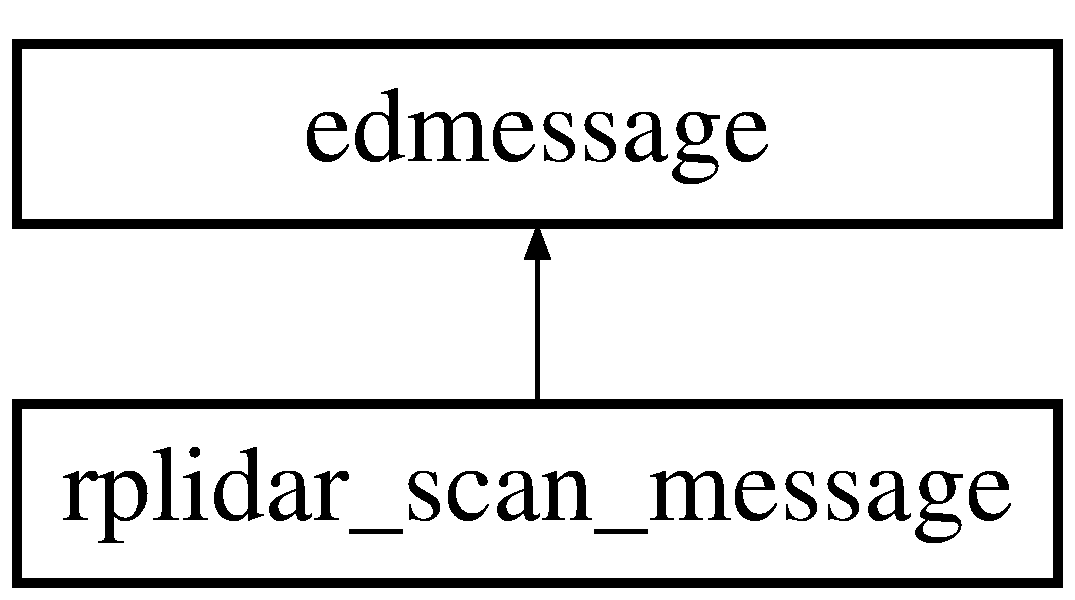
\includegraphics[height=2.000000cm]{structrplidar__scan__message}
\end{center}
\end{figure}
\subsection*{Public Member Functions}
\begin{DoxyCompactItemize}
\item 
virtual std\-::string \hyperlink{structrplidar__scan__message_aa402778fbabf5375a2a9f229bdb609b6}{type} ()
\end{DoxyCompactItemize}
\subsection*{Static Public Member Functions}
\begin{DoxyCompactItemize}
\item 
static std\-::string \hyperlink{structrplidar__scan__message_a9df9e3d712a557d2f4abc3c90c5907b7}{Type} ()
\end{DoxyCompactItemize}
\subsection*{Public Attributes}
\begin{DoxyCompactItemize}
\item 
\hyperlink{structcomplete__scan__data__packet}{complete\-\_\-scan\-\_\-data\-\_\-packet} \hyperlink{structrplidar__scan__message_a93aed58534e2f3b8263c3a27e4b1f511}{scan\-\_\-data}
\item 
uint32\-\_\-t \hyperlink{structrplidar__scan__message_a8a3d08350e35f717ef463ee0ee6f6952}{millis\-\_\-timestamp}
\end{DoxyCompactItemize}


\subsection{Member Function Documentation}
\hypertarget{structrplidar__scan__message_aa402778fbabf5375a2a9f229bdb609b6}{\index{rplidar\-\_\-scan\-\_\-message@{rplidar\-\_\-scan\-\_\-message}!type@{type}}
\index{type@{type}!rplidar_scan_message@{rplidar\-\_\-scan\-\_\-message}}
\subsubsection[{type}]{\setlength{\rightskip}{0pt plus 5cm}virtual std\-::string rplidar\-\_\-scan\-\_\-message\-::type (
\begin{DoxyParamCaption}
{}
\end{DoxyParamCaption}
)\hspace{0.3cm}{\ttfamily [inline]}, {\ttfamily [virtual]}}}\label{structrplidar__scan__message_aa402778fbabf5375a2a9f229bdb609b6}


Implements \hyperlink{structedmessage_ac888cf8e570a4aa9bea30a4c4fcdcc30}{edmessage}.

\hypertarget{structrplidar__scan__message_a9df9e3d712a557d2f4abc3c90c5907b7}{\index{rplidar\-\_\-scan\-\_\-message@{rplidar\-\_\-scan\-\_\-message}!Type@{Type}}
\index{Type@{Type}!rplidar_scan_message@{rplidar\-\_\-scan\-\_\-message}}
\subsubsection[{Type}]{\setlength{\rightskip}{0pt plus 5cm}static std\-::string rplidar\-\_\-scan\-\_\-message\-::\-Type (
\begin{DoxyParamCaption}
{}
\end{DoxyParamCaption}
)\hspace{0.3cm}{\ttfamily [inline]}, {\ttfamily [static]}}}\label{structrplidar__scan__message_a9df9e3d712a557d2f4abc3c90c5907b7}


\subsection{Member Data Documentation}
\hypertarget{structrplidar__scan__message_a8a3d08350e35f717ef463ee0ee6f6952}{\index{rplidar\-\_\-scan\-\_\-message@{rplidar\-\_\-scan\-\_\-message}!millis\-\_\-timestamp@{millis\-\_\-timestamp}}
\index{millis\-\_\-timestamp@{millis\-\_\-timestamp}!rplidar_scan_message@{rplidar\-\_\-scan\-\_\-message}}
\subsubsection[{millis\-\_\-timestamp}]{\setlength{\rightskip}{0pt plus 5cm}uint32\-\_\-t rplidar\-\_\-scan\-\_\-message\-::millis\-\_\-timestamp}}\label{structrplidar__scan__message_a8a3d08350e35f717ef463ee0ee6f6952}
\hypertarget{structrplidar__scan__message_a93aed58534e2f3b8263c3a27e4b1f511}{\index{rplidar\-\_\-scan\-\_\-message@{rplidar\-\_\-scan\-\_\-message}!scan\-\_\-data@{scan\-\_\-data}}
\index{scan\-\_\-data@{scan\-\_\-data}!rplidar_scan_message@{rplidar\-\_\-scan\-\_\-message}}
\subsubsection[{scan\-\_\-data}]{\setlength{\rightskip}{0pt plus 5cm}{\bf complete\-\_\-scan\-\_\-data\-\_\-packet} rplidar\-\_\-scan\-\_\-message\-::scan\-\_\-data}}\label{structrplidar__scan__message_a93aed58534e2f3b8263c3a27e4b1f511}


The documentation for this struct was generated from the following file\-:\begin{DoxyCompactItemize}
\item 
/home/dprandle/\-Documents/code/ctrlmod/include/\hyperlink{edmessage_8h}{edmessage.\-h}\end{DoxyCompactItemize}

\hypertarget{structscan__data__packet}{\section{scan\-\_\-data\-\_\-packet Struct Reference}
\label{structscan__data__packet}\index{scan\-\_\-data\-\_\-packet@{scan\-\_\-data\-\_\-packet}}
}


{\ttfamily \#include $<$edrplidar\-\_\-packets.\-h$>$}

Inheritance diagram for scan\-\_\-data\-\_\-packet\-:\begin{figure}[H]
\begin{center}
\leavevmode
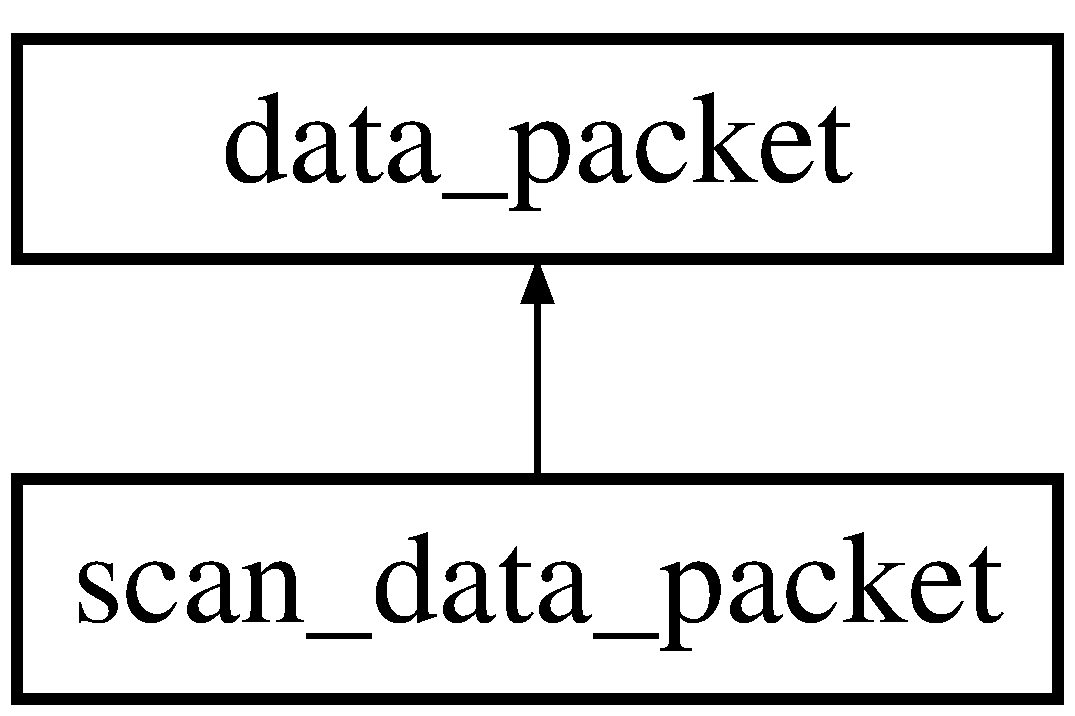
\includegraphics[height=2.000000cm]{structscan__data__packet}
\end{center}
\end{figure}
\subsection*{Public Member Functions}
\begin{DoxyCompactItemize}
\item 
\hyperlink{structscan__data__packet_a991911b1c806c6b288baa4b7b95d8e1d}{scan\-\_\-data\-\_\-packet} ()
\item 
virtual std\-::string \hyperlink{structscan__data__packet_aa8d4b795a798f413149c93760de6577f}{to\-String} ()
\item 
std\-::string \hyperlink{structscan__data__packet_a8401263b8927ca5a67ca23c8797cc67e}{type} ()
\item 
virtual uint32\-\_\-t \hyperlink{structscan__data__packet_a2678e9313e25c529abba1c1ba5ff3cba}{size} ()
\item 
virtual uint8\-\_\-t \& \hyperlink{structscan__data__packet_ac8b9b314239dd2663a7d2b98e5cd1c1a}{operator\mbox{[}$\,$\mbox{]}} (uint32\-\_\-t index)
\item 
virtual uint8\-\_\-t $\ast$ \hyperlink{structscan__data__packet_a376edae10eddfa50b3684e801a0a8f3a}{dataptr} ()
\end{DoxyCompactItemize}
\subsection*{Static Public Member Functions}
\begin{DoxyCompactItemize}
\item 
static std\-::string \hyperlink{structscan__data__packet_add0b207133c083ddbea5a2d7c094baba}{Type} ()
\item 
static uint32\-\_\-t \hyperlink{structscan__data__packet_a383d91432a45ada918769e2737b9593e}{Size} ()
\end{DoxyCompactItemize}
\subsection*{Public Attributes}
\begin{DoxyCompactItemize}
\item 
\begin{tabbing}
xx\=xx\=xx\=xx\=xx\=xx\=xx\=xx\=xx\=\kill
union \{\\
\>struct \{\\
\>\>uint8\_t \hyperlink{structscan__data__packet_af592db980953da3509611b9d5176cd8e}{qual\_s\_sn}\\
\>\>uint8\_t \hyperlink{structscan__data__packet_afa912fe10cbd68a6b8a60df2a1faa3ba}{angle6to0\_C}\\
\>\>uint8\_t \hyperlink{structscan__data__packet_a614148a4a3e77048b6dd004e6e37c858}{angle14to7}\\
\>\>uint8\_t \hyperlink{structscan__data__packet_a1622768a34e474d4ea482bd8ad27849f}{distance7to0}\\
\>\>uint8\_t \hyperlink{structscan__data__packet_ae144f4bb4a3022fdfdb513959f0fd668}{distance15to8}\\
\>\} \\
\>uint8\_t \hyperlink{structscan__data__packet_ab2de61ce3719327366ee913c9a6b58fc}{data} \mbox{[}5\mbox{]}\\
\}; \\

\end{tabbing}\end{DoxyCompactItemize}


\subsection{Constructor \& Destructor Documentation}
\hypertarget{structscan__data__packet_a991911b1c806c6b288baa4b7b95d8e1d}{\index{scan\-\_\-data\-\_\-packet@{scan\-\_\-data\-\_\-packet}!scan\-\_\-data\-\_\-packet@{scan\-\_\-data\-\_\-packet}}
\index{scan\-\_\-data\-\_\-packet@{scan\-\_\-data\-\_\-packet}!scan_data_packet@{scan\-\_\-data\-\_\-packet}}
\subsubsection[{scan\-\_\-data\-\_\-packet}]{\setlength{\rightskip}{0pt plus 5cm}scan\-\_\-data\-\_\-packet\-::scan\-\_\-data\-\_\-packet (
\begin{DoxyParamCaption}
{}
\end{DoxyParamCaption}
)}}\label{structscan__data__packet_a991911b1c806c6b288baa4b7b95d8e1d}


\subsection{Member Function Documentation}
\hypertarget{structscan__data__packet_a376edae10eddfa50b3684e801a0a8f3a}{\index{scan\-\_\-data\-\_\-packet@{scan\-\_\-data\-\_\-packet}!dataptr@{dataptr}}
\index{dataptr@{dataptr}!scan_data_packet@{scan\-\_\-data\-\_\-packet}}
\subsubsection[{dataptr}]{\setlength{\rightskip}{0pt plus 5cm}virtual uint8\-\_\-t$\ast$ scan\-\_\-data\-\_\-packet\-::dataptr (
\begin{DoxyParamCaption}
{}
\end{DoxyParamCaption}
)\hspace{0.3cm}{\ttfamily [inline]}, {\ttfamily [virtual]}}}\label{structscan__data__packet_a376edae10eddfa50b3684e801a0a8f3a}


Implements \hyperlink{structdata__packet_ac53dcca572fc7cf7d71ae21d5c785365}{data\-\_\-packet}.

\hypertarget{structscan__data__packet_ac8b9b314239dd2663a7d2b98e5cd1c1a}{\index{scan\-\_\-data\-\_\-packet@{scan\-\_\-data\-\_\-packet}!operator\mbox{[}$\,$\mbox{]}@{operator[]}}
\index{operator\mbox{[}$\,$\mbox{]}@{operator[]}!scan_data_packet@{scan\-\_\-data\-\_\-packet}}
\subsubsection[{operator[]}]{\setlength{\rightskip}{0pt plus 5cm}virtual uint8\-\_\-t\& scan\-\_\-data\-\_\-packet\-::operator\mbox{[}$\,$\mbox{]} (
\begin{DoxyParamCaption}
\item[{uint32\-\_\-t}]{index}
\end{DoxyParamCaption}
)\hspace{0.3cm}{\ttfamily [inline]}, {\ttfamily [virtual]}}}\label{structscan__data__packet_ac8b9b314239dd2663a7d2b98e5cd1c1a}


Implements \hyperlink{structdata__packet_a8f0d95d4a7a7089b45cef14e45b0c21b}{data\-\_\-packet}.

\hypertarget{structscan__data__packet_a2678e9313e25c529abba1c1ba5ff3cba}{\index{scan\-\_\-data\-\_\-packet@{scan\-\_\-data\-\_\-packet}!size@{size}}
\index{size@{size}!scan_data_packet@{scan\-\_\-data\-\_\-packet}}
\subsubsection[{size}]{\setlength{\rightskip}{0pt plus 5cm}virtual uint32\-\_\-t scan\-\_\-data\-\_\-packet\-::size (
\begin{DoxyParamCaption}
{}
\end{DoxyParamCaption}
)\hspace{0.3cm}{\ttfamily [inline]}, {\ttfamily [virtual]}}}\label{structscan__data__packet_a2678e9313e25c529abba1c1ba5ff3cba}


Implements \hyperlink{structdata__packet_ab5c9259a79cde0dc60d75135fe8464f6}{data\-\_\-packet}.

\hypertarget{structscan__data__packet_a383d91432a45ada918769e2737b9593e}{\index{scan\-\_\-data\-\_\-packet@{scan\-\_\-data\-\_\-packet}!Size@{Size}}
\index{Size@{Size}!scan_data_packet@{scan\-\_\-data\-\_\-packet}}
\subsubsection[{Size}]{\setlength{\rightskip}{0pt plus 5cm}static uint32\-\_\-t scan\-\_\-data\-\_\-packet\-::\-Size (
\begin{DoxyParamCaption}
{}
\end{DoxyParamCaption}
)\hspace{0.3cm}{\ttfamily [inline]}, {\ttfamily [static]}}}\label{structscan__data__packet_a383d91432a45ada918769e2737b9593e}
\hypertarget{structscan__data__packet_aa8d4b795a798f413149c93760de6577f}{\index{scan\-\_\-data\-\_\-packet@{scan\-\_\-data\-\_\-packet}!to\-String@{to\-String}}
\index{to\-String@{to\-String}!scan_data_packet@{scan\-\_\-data\-\_\-packet}}
\subsubsection[{to\-String}]{\setlength{\rightskip}{0pt plus 5cm}std\-::string scan\-\_\-data\-\_\-packet\-::to\-String (
\begin{DoxyParamCaption}
{}
\end{DoxyParamCaption}
)\hspace{0.3cm}{\ttfamily [virtual]}}}\label{structscan__data__packet_aa8d4b795a798f413149c93760de6577f}


Implements \hyperlink{structdata__packet_ad7ce179caef76c895bfc778862bc15ac}{data\-\_\-packet}.

\hypertarget{structscan__data__packet_a8401263b8927ca5a67ca23c8797cc67e}{\index{scan\-\_\-data\-\_\-packet@{scan\-\_\-data\-\_\-packet}!type@{type}}
\index{type@{type}!scan_data_packet@{scan\-\_\-data\-\_\-packet}}
\subsubsection[{type}]{\setlength{\rightskip}{0pt plus 5cm}std\-::string scan\-\_\-data\-\_\-packet\-::type (
\begin{DoxyParamCaption}
{}
\end{DoxyParamCaption}
)\hspace{0.3cm}{\ttfamily [inline]}, {\ttfamily [virtual]}}}\label{structscan__data__packet_a8401263b8927ca5a67ca23c8797cc67e}


Implements \hyperlink{structdata__packet_af0795581f2d57a8c14a88009da37aee1}{data\-\_\-packet}.

\hypertarget{structscan__data__packet_add0b207133c083ddbea5a2d7c094baba}{\index{scan\-\_\-data\-\_\-packet@{scan\-\_\-data\-\_\-packet}!Type@{Type}}
\index{Type@{Type}!scan_data_packet@{scan\-\_\-data\-\_\-packet}}
\subsubsection[{Type}]{\setlength{\rightskip}{0pt plus 5cm}static std\-::string scan\-\_\-data\-\_\-packet\-::\-Type (
\begin{DoxyParamCaption}
{}
\end{DoxyParamCaption}
)\hspace{0.3cm}{\ttfamily [inline]}, {\ttfamily [static]}}}\label{structscan__data__packet_add0b207133c083ddbea5a2d7c094baba}


\subsection{Member Data Documentation}
\hypertarget{structscan__data__packet_a4f10bb28fada5dc58732724f356e68d2}{\subsubsection[{"@13}]{\setlength{\rightskip}{0pt plus 5cm}union \{ ... \} }}\label{structscan__data__packet_a4f10bb28fada5dc58732724f356e68d2}
\hypertarget{structscan__data__packet_a614148a4a3e77048b6dd004e6e37c858}{\index{scan\-\_\-data\-\_\-packet@{scan\-\_\-data\-\_\-packet}!angle14to7@{angle14to7}}
\index{angle14to7@{angle14to7}!scan_data_packet@{scan\-\_\-data\-\_\-packet}}
\subsubsection[{angle14to7}]{\setlength{\rightskip}{0pt plus 5cm}uint8\-\_\-t scan\-\_\-data\-\_\-packet\-::angle14to7}}\label{structscan__data__packet_a614148a4a3e77048b6dd004e6e37c858}
\hypertarget{structscan__data__packet_afa912fe10cbd68a6b8a60df2a1faa3ba}{\index{scan\-\_\-data\-\_\-packet@{scan\-\_\-data\-\_\-packet}!angle6to0\-\_\-\-C@{angle6to0\-\_\-\-C}}
\index{angle6to0\-\_\-\-C@{angle6to0\-\_\-\-C}!scan_data_packet@{scan\-\_\-data\-\_\-packet}}
\subsubsection[{angle6to0\-\_\-\-C}]{\setlength{\rightskip}{0pt plus 5cm}uint8\-\_\-t scan\-\_\-data\-\_\-packet\-::angle6to0\-\_\-\-C}}\label{structscan__data__packet_afa912fe10cbd68a6b8a60df2a1faa3ba}
\hypertarget{structscan__data__packet_ab2de61ce3719327366ee913c9a6b58fc}{\index{scan\-\_\-data\-\_\-packet@{scan\-\_\-data\-\_\-packet}!data@{data}}
\index{data@{data}!scan_data_packet@{scan\-\_\-data\-\_\-packet}}
\subsubsection[{data}]{\setlength{\rightskip}{0pt plus 5cm}uint8\-\_\-t scan\-\_\-data\-\_\-packet\-::data\mbox{[}5\mbox{]}}}\label{structscan__data__packet_ab2de61ce3719327366ee913c9a6b58fc}
\hypertarget{structscan__data__packet_ae144f4bb4a3022fdfdb513959f0fd668}{\index{scan\-\_\-data\-\_\-packet@{scan\-\_\-data\-\_\-packet}!distance15to8@{distance15to8}}
\index{distance15to8@{distance15to8}!scan_data_packet@{scan\-\_\-data\-\_\-packet}}
\subsubsection[{distance15to8}]{\setlength{\rightskip}{0pt plus 5cm}uint8\-\_\-t scan\-\_\-data\-\_\-packet\-::distance15to8}}\label{structscan__data__packet_ae144f4bb4a3022fdfdb513959f0fd668}
\hypertarget{structscan__data__packet_a1622768a34e474d4ea482bd8ad27849f}{\index{scan\-\_\-data\-\_\-packet@{scan\-\_\-data\-\_\-packet}!distance7to0@{distance7to0}}
\index{distance7to0@{distance7to0}!scan_data_packet@{scan\-\_\-data\-\_\-packet}}
\subsubsection[{distance7to0}]{\setlength{\rightskip}{0pt plus 5cm}uint8\-\_\-t scan\-\_\-data\-\_\-packet\-::distance7to0}}\label{structscan__data__packet_a1622768a34e474d4ea482bd8ad27849f}
\hypertarget{structscan__data__packet_af592db980953da3509611b9d5176cd8e}{\index{scan\-\_\-data\-\_\-packet@{scan\-\_\-data\-\_\-packet}!qual\-\_\-s\-\_\-sn@{qual\-\_\-s\-\_\-sn}}
\index{qual\-\_\-s\-\_\-sn@{qual\-\_\-s\-\_\-sn}!scan_data_packet@{scan\-\_\-data\-\_\-packet}}
\subsubsection[{qual\-\_\-s\-\_\-sn}]{\setlength{\rightskip}{0pt plus 5cm}uint8\-\_\-t scan\-\_\-data\-\_\-packet\-::qual\-\_\-s\-\_\-sn}}\label{structscan__data__packet_af592db980953da3509611b9d5176cd8e}


The documentation for this struct was generated from the following files\-:\begin{DoxyCompactItemize}
\item 
/home/dprandle/\-Documents/code/ctrlmod/include/\hyperlink{edrplidar__packets_8h}{edrplidar\-\_\-packets.\-h}\item 
/home/dprandle/\-Documents/code/ctrlmod/src/\hyperlink{edrplidar__packets_8cpp}{edrplidar\-\_\-packets.\-cpp}\end{DoxyCompactItemize}

\hypertarget{structscan__descriptor}{\section{scan\-\_\-descriptor Struct Reference}
\label{structscan__descriptor}\index{scan\-\_\-descriptor@{scan\-\_\-descriptor}}
}


{\ttfamily \#include $<$edrplidar\-\_\-packets.\-h$>$}

Inheritance diagram for scan\-\_\-descriptor\-:\begin{figure}[H]
\begin{center}
\leavevmode
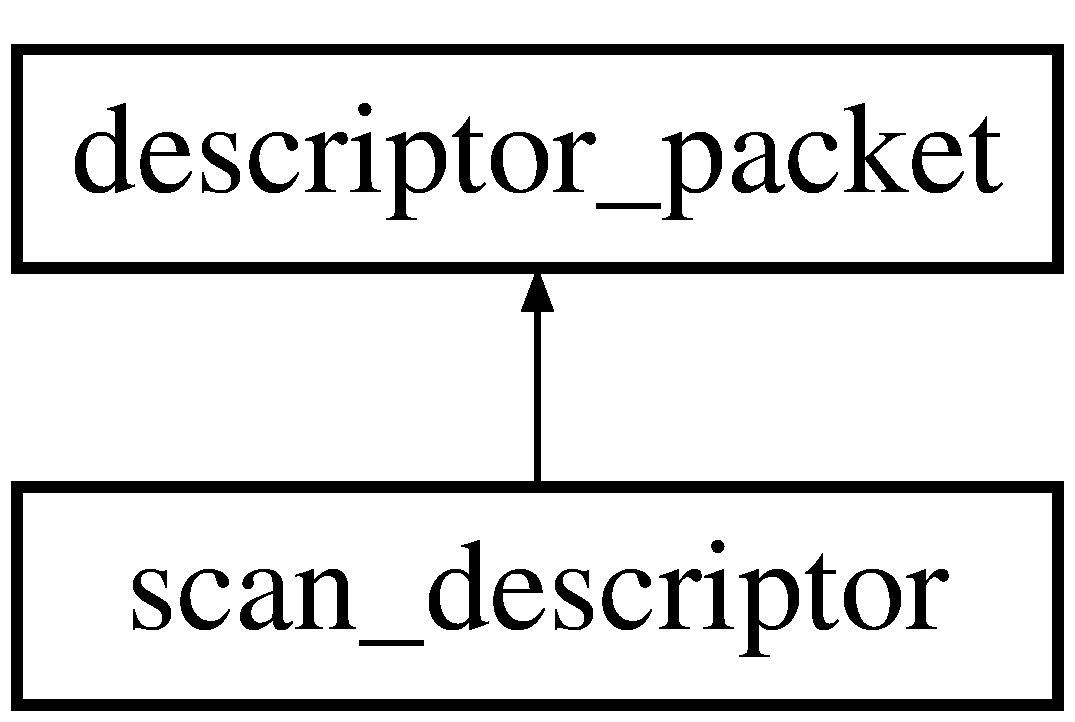
\includegraphics[height=2.000000cm]{structscan__descriptor}
\end{center}
\end{figure}
\subsection*{Public Member Functions}
\begin{DoxyCompactItemize}
\item 
\hyperlink{structscan__descriptor_a87b90f4822193f3cbaf176109093b709}{scan\-\_\-descriptor} ()
\item 
virtual std\-::string \hyperlink{structscan__descriptor_a3020edbf9b9ff7e8c50a150050e0ec6f}{type} ()
\end{DoxyCompactItemize}
\subsection*{Additional Inherited Members}


\subsection{Constructor \& Destructor Documentation}
\hypertarget{structscan__descriptor_a87b90f4822193f3cbaf176109093b709}{\index{scan\-\_\-descriptor@{scan\-\_\-descriptor}!scan\-\_\-descriptor@{scan\-\_\-descriptor}}
\index{scan\-\_\-descriptor@{scan\-\_\-descriptor}!scan_descriptor@{scan\-\_\-descriptor}}
\subsubsection[{scan\-\_\-descriptor}]{\setlength{\rightskip}{0pt plus 5cm}scan\-\_\-descriptor\-::scan\-\_\-descriptor (
\begin{DoxyParamCaption}
{}
\end{DoxyParamCaption}
)\hspace{0.3cm}{\ttfamily [inline]}}}\label{structscan__descriptor_a87b90f4822193f3cbaf176109093b709}


\subsection{Member Function Documentation}
\hypertarget{structscan__descriptor_a3020edbf9b9ff7e8c50a150050e0ec6f}{\index{scan\-\_\-descriptor@{scan\-\_\-descriptor}!type@{type}}
\index{type@{type}!scan_descriptor@{scan\-\_\-descriptor}}
\subsubsection[{type}]{\setlength{\rightskip}{0pt plus 5cm}virtual std\-::string scan\-\_\-descriptor\-::type (
\begin{DoxyParamCaption}
{}
\end{DoxyParamCaption}
)\hspace{0.3cm}{\ttfamily [inline]}, {\ttfamily [virtual]}}}\label{structscan__descriptor_a3020edbf9b9ff7e8c50a150050e0ec6f}


Implements \hyperlink{structdescriptor__packet_ad08369aae987f91544cee5e8f2267f2f}{descriptor\-\_\-packet}.



The documentation for this struct was generated from the following file\-:\begin{DoxyCompactItemize}
\item 
/home/dprandle/\-Documents/code/ctrlmod/include/\hyperlink{edrplidar__packets_8h}{edrplidar\-\_\-packets.\-h}\end{DoxyCompactItemize}

\hypertarget{structstart__scan__request}{\section{start\-\_\-scan\-\_\-request Struct Reference}
\label{structstart__scan__request}\index{start\-\_\-scan\-\_\-request@{start\-\_\-scan\-\_\-request}}
}


{\ttfamily \#include $<$edrplidar\-\_\-packets.\-h$>$}

Inheritance diagram for start\-\_\-scan\-\_\-request\-:\begin{figure}[H]
\begin{center}
\leavevmode
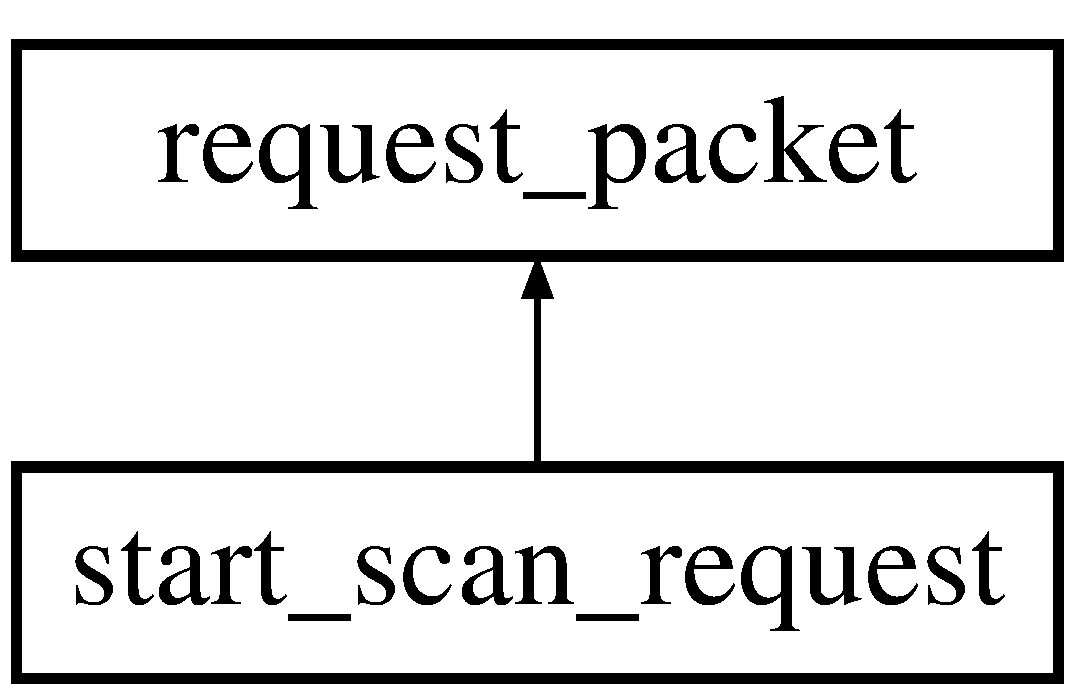
\includegraphics[height=2.000000cm]{structstart__scan__request}
\end{center}
\end{figure}
\subsection*{Public Member Functions}
\begin{DoxyCompactItemize}
\item 
\hyperlink{structstart__scan__request_a5ab81d664805c9fb5b09e77e07f17b27}{start\-\_\-scan\-\_\-request} ()
\end{DoxyCompactItemize}
\subsection*{Additional Inherited Members}


\subsection{Constructor \& Destructor Documentation}
\hypertarget{structstart__scan__request_a5ab81d664805c9fb5b09e77e07f17b27}{\index{start\-\_\-scan\-\_\-request@{start\-\_\-scan\-\_\-request}!start\-\_\-scan\-\_\-request@{start\-\_\-scan\-\_\-request}}
\index{start\-\_\-scan\-\_\-request@{start\-\_\-scan\-\_\-request}!start_scan_request@{start\-\_\-scan\-\_\-request}}
\subsubsection[{start\-\_\-scan\-\_\-request}]{\setlength{\rightskip}{0pt plus 5cm}start\-\_\-scan\-\_\-request\-::start\-\_\-scan\-\_\-request (
\begin{DoxyParamCaption}
{}
\end{DoxyParamCaption}
)\hspace{0.3cm}{\ttfamily [inline]}}}\label{structstart__scan__request_a5ab81d664805c9fb5b09e77e07f17b27}


The documentation for this struct was generated from the following file\-:\begin{DoxyCompactItemize}
\item 
/home/dprandle/\-Documents/code/ctrlmod/include/\hyperlink{edrplidar__packets_8h}{edrplidar\-\_\-packets.\-h}\end{DoxyCompactItemize}

\hypertarget{structstop__scan__request}{\section{stop\-\_\-scan\-\_\-request Struct Reference}
\label{structstop__scan__request}\index{stop\-\_\-scan\-\_\-request@{stop\-\_\-scan\-\_\-request}}
}


{\ttfamily \#include $<$edrplidar\-\_\-packets.\-h$>$}

Inheritance diagram for stop\-\_\-scan\-\_\-request\-:\begin{figure}[H]
\begin{center}
\leavevmode
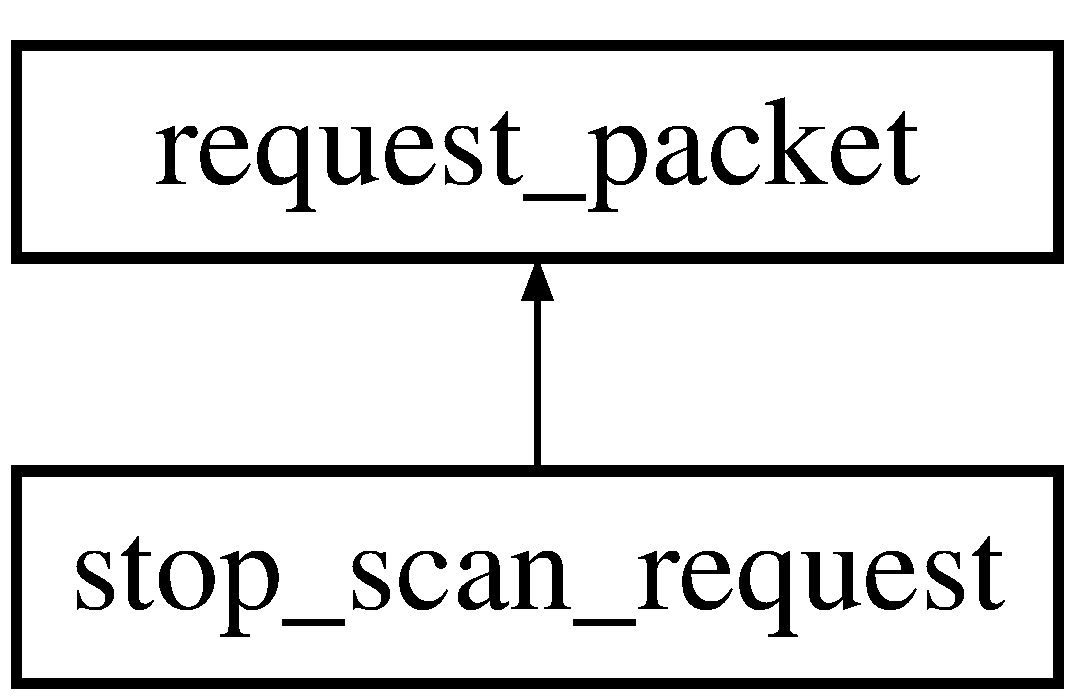
\includegraphics[height=2.000000cm]{structstop__scan__request}
\end{center}
\end{figure}
\subsection*{Public Member Functions}
\begin{DoxyCompactItemize}
\item 
\hyperlink{structstop__scan__request_a91e85678d9163896274363364924cbc0}{stop\-\_\-scan\-\_\-request} ()
\end{DoxyCompactItemize}
\subsection*{Additional Inherited Members}


\subsection{Constructor \& Destructor Documentation}
\hypertarget{structstop__scan__request_a91e85678d9163896274363364924cbc0}{\index{stop\-\_\-scan\-\_\-request@{stop\-\_\-scan\-\_\-request}!stop\-\_\-scan\-\_\-request@{stop\-\_\-scan\-\_\-request}}
\index{stop\-\_\-scan\-\_\-request@{stop\-\_\-scan\-\_\-request}!stop_scan_request@{stop\-\_\-scan\-\_\-request}}
\subsubsection[{stop\-\_\-scan\-\_\-request}]{\setlength{\rightskip}{0pt plus 5cm}stop\-\_\-scan\-\_\-request\-::stop\-\_\-scan\-\_\-request (
\begin{DoxyParamCaption}
{}
\end{DoxyParamCaption}
)\hspace{0.3cm}{\ttfamily [inline]}}}\label{structstop__scan__request_a91e85678d9163896274363364924cbc0}


The documentation for this struct was generated from the following file\-:\begin{DoxyCompactItemize}
\item 
/home/dprandle/\-Documents/code/ctrlmod/include/\hyperlink{edrplidar__packets_8h}{edrplidar\-\_\-packets.\-h}\end{DoxyCompactItemize}

\hypertarget{structwait__ready__callback}{\section{wait\-\_\-ready\-\_\-callback Struct Reference}
\label{structwait__ready__callback}\index{wait\-\_\-ready\-\_\-callback@{wait\-\_\-ready\-\_\-callback}}
}


{\ttfamily \#include $<$edcallback.\-h$>$}

Inheritance diagram for wait\-\_\-ready\-\_\-callback\-:\begin{figure}[H]
\begin{center}
\leavevmode
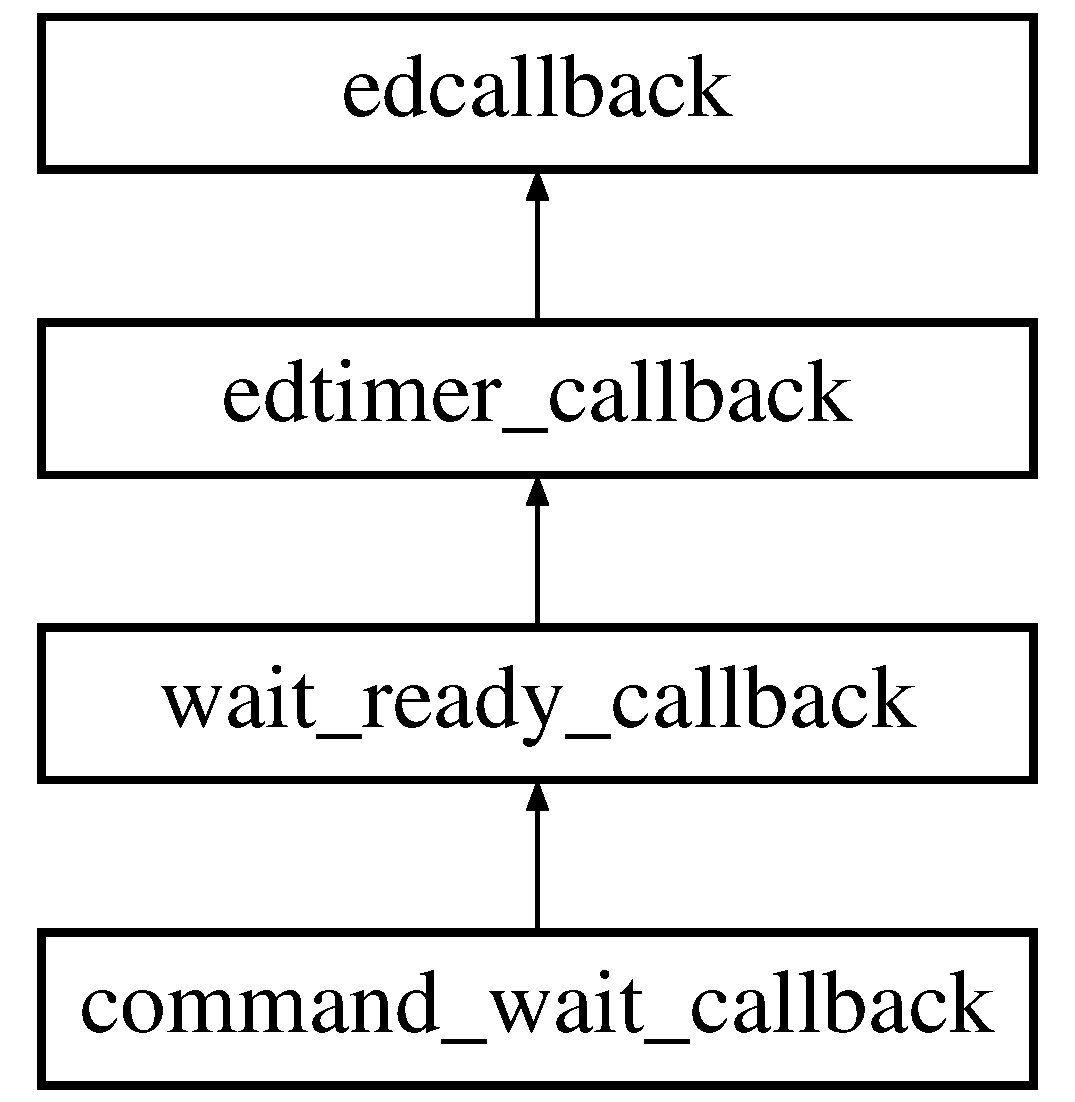
\includegraphics[height=4.000000cm]{structwait__ready__callback}
\end{center}
\end{figure}
\subsection*{Public Member Functions}
\begin{DoxyCompactItemize}
\item 
virtual void \hyperlink{structwait__ready__callback_a305d57ffdd8bc5d3682dfa4a83431708}{exec} ()
\end{DoxyCompactItemize}
\subsection*{Additional Inherited Members}


\subsection{Member Function Documentation}
\hypertarget{structwait__ready__callback_a305d57ffdd8bc5d3682dfa4a83431708}{\index{wait\-\_\-ready\-\_\-callback@{wait\-\_\-ready\-\_\-callback}!exec@{exec}}
\index{exec@{exec}!wait_ready_callback@{wait\-\_\-ready\-\_\-callback}}
\subsubsection[{exec}]{\setlength{\rightskip}{0pt plus 5cm}void wait\-\_\-ready\-\_\-callback\-::exec (
\begin{DoxyParamCaption}
{}
\end{DoxyParamCaption}
)\hspace{0.3cm}{\ttfamily [virtual]}}}\label{structwait__ready__callback_a305d57ffdd8bc5d3682dfa4a83431708}


Implements \hyperlink{structedcallback_ab8003af2178e58a94f53370b1f48a313}{edcallback}.



Reimplemented in \hyperlink{structcommand__wait__callback_ae5ab034230cd73f6203cee386ba1993c}{command\-\_\-wait\-\_\-callback}.



The documentation for this struct was generated from the following files\-:\begin{DoxyCompactItemize}
\item 
/home/dprandle/\-Documents/code/ctrlmod/include/\hyperlink{edcallback_8h}{edcallback.\-h}\item 
/home/dprandle/\-Documents/code/ctrlmod/src/\hyperlink{edcallback_8cpp}{edcallback.\-cpp}\end{DoxyCompactItemize}

\hypertarget{structedthreaded__fd_1_1WriteVal}{\section{edthreaded\-\_\-fd\-:\-:Write\-Val Struct Reference}
\label{structedthreaded__fd_1_1WriteVal}\index{edthreaded\-\_\-fd\-::\-Write\-Val@{edthreaded\-\_\-fd\-::\-Write\-Val}}
}


{\ttfamily \#include $<$edthreaded\-\_\-fd.\-h$>$}

\subsection*{Public Member Functions}
\begin{DoxyCompactItemize}
\item 
\hyperlink{structedthreaded__fd_1_1WriteVal_a2e44699eec697ffa373f6633a0d85f92}{Write\-Val} (uint8\-\_\-t byte\-\_\-=0x00, int32\-\_\-t response\-\_\-size\-\_\-=0)
\end{DoxyCompactItemize}
\subsection*{Public Attributes}
\begin{DoxyCompactItemize}
\item 
uint8\-\_\-t \hyperlink{structedthreaded__fd_1_1WriteVal_abddfddda0a4db161d604a6d928fc275e}{byte}
\item 
uint32\-\_\-t \hyperlink{structedthreaded__fd_1_1WriteVal_abc008bb97658cfd09ed941c266b1168d}{response\-\_\-size}
\end{DoxyCompactItemize}


\subsection{Constructor \& Destructor Documentation}
\hypertarget{structedthreaded__fd_1_1WriteVal_a2e44699eec697ffa373f6633a0d85f92}{\index{edthreaded\-\_\-fd\-::\-Write\-Val@{edthreaded\-\_\-fd\-::\-Write\-Val}!Write\-Val@{Write\-Val}}
\index{Write\-Val@{Write\-Val}!edthreaded_fd::WriteVal@{edthreaded\-\_\-fd\-::\-Write\-Val}}
\subsubsection[{Write\-Val}]{\setlength{\rightskip}{0pt plus 5cm}edthreaded\-\_\-fd\-::\-Write\-Val\-::\-Write\-Val (
\begin{DoxyParamCaption}
\item[{uint8\-\_\-t}]{byte\-\_\- = {\ttfamily 0x00}, }
\item[{int32\-\_\-t}]{response\-\_\-size\-\_\- = {\ttfamily 0}}
\end{DoxyParamCaption}
)\hspace{0.3cm}{\ttfamily [inline]}}}\label{structedthreaded__fd_1_1WriteVal_a2e44699eec697ffa373f6633a0d85f92}


\subsection{Member Data Documentation}
\hypertarget{structedthreaded__fd_1_1WriteVal_abddfddda0a4db161d604a6d928fc275e}{\index{edthreaded\-\_\-fd\-::\-Write\-Val@{edthreaded\-\_\-fd\-::\-Write\-Val}!byte@{byte}}
\index{byte@{byte}!edthreaded_fd::WriteVal@{edthreaded\-\_\-fd\-::\-Write\-Val}}
\subsubsection[{byte}]{\setlength{\rightskip}{0pt plus 5cm}uint8\-\_\-t edthreaded\-\_\-fd\-::\-Write\-Val\-::byte}}\label{structedthreaded__fd_1_1WriteVal_abddfddda0a4db161d604a6d928fc275e}
\hypertarget{structedthreaded__fd_1_1WriteVal_abc008bb97658cfd09ed941c266b1168d}{\index{edthreaded\-\_\-fd\-::\-Write\-Val@{edthreaded\-\_\-fd\-::\-Write\-Val}!response\-\_\-size@{response\-\_\-size}}
\index{response\-\_\-size@{response\-\_\-size}!edthreaded_fd::WriteVal@{edthreaded\-\_\-fd\-::\-Write\-Val}}
\subsubsection[{response\-\_\-size}]{\setlength{\rightskip}{0pt plus 5cm}uint32\-\_\-t edthreaded\-\_\-fd\-::\-Write\-Val\-::response\-\_\-size}}\label{structedthreaded__fd_1_1WriteVal_abc008bb97658cfd09ed941c266b1168d}


The documentation for this struct was generated from the following file\-:\begin{DoxyCompactItemize}
\item 
/home/dprandle/\-Documents/code/ctrlmod/include/\hyperlink{edthreaded__fd_8h}{edthreaded\-\_\-fd.\-h}\end{DoxyCompactItemize}

\chapter{File Documentation}
\hypertarget{edcallback_8h}{\section{/home/dprandle/\-Documents/code/ctrlmod/include/edcallback.h File Reference}
\label{edcallback_8h}\index{/home/dprandle/\-Documents/code/ctrlmod/include/edcallback.\-h@{/home/dprandle/\-Documents/code/ctrlmod/include/edcallback.\-h}}
}
\subsection*{Classes}
\begin{DoxyCompactItemize}
\item 
struct \hyperlink{structedcallback}{edcallback}
\item 
struct \hyperlink{structedtimer__callback}{edtimer\-\_\-callback}
\item 
struct \hyperlink{structwait__ready__callback}{wait\-\_\-ready\-\_\-callback}
\end{DoxyCompactItemize}

\hypertarget{edcomm__system_8h}{\section{/home/dprandle/\-Documents/code/ctrlmod/include/edcomm\-\_\-system.h File Reference}
\label{edcomm__system_8h}\index{/home/dprandle/\-Documents/code/ctrlmod/include/edcomm\-\_\-system.\-h@{/home/dprandle/\-Documents/code/ctrlmod/include/edcomm\-\_\-system.\-h}}
}
{\ttfamily \#include $<$edglobal.\-h$>$}\\*
{\ttfamily \#include $<$edsystem.\-h$>$}\\*
{\ttfamily \#include $<$vector$>$}\\*
\subsection*{Classes}
\begin{DoxyCompactItemize}
\item 
struct \hyperlink{structCommand}{Command}
\item 
class \hyperlink{classedcomm__system}{edcomm\-\_\-system}
\end{DoxyCompactItemize}
\subsection*{Macros}
\begin{DoxyCompactItemize}
\item 
\#define \hyperlink{edcomm__system_8h_a64dd4834292846960f8ab21e3940bb64}{S\-O\-C\-K\-E\-T\-\_\-\-B\-U\-F\-F\-\_\-\-S\-I\-Z\-E}
\item 
\#define \hyperlink{edcomm__system_8h_a0d1ec489be62a2310c9725ac6164abdb}{C\-O\-M\-M\-A\-N\-D\-\_\-\-B\-Y\-T\-E\-\_\-\-S\-I\-Z\-E}~72
\end{DoxyCompactItemize}


\subsection{Macro Definition Documentation}
\hypertarget{edcomm__system_8h_a0d1ec489be62a2310c9725ac6164abdb}{\index{edcomm\-\_\-system.\-h@{edcomm\-\_\-system.\-h}!C\-O\-M\-M\-A\-N\-D\-\_\-\-B\-Y\-T\-E\-\_\-\-S\-I\-Z\-E@{C\-O\-M\-M\-A\-N\-D\-\_\-\-B\-Y\-T\-E\-\_\-\-S\-I\-Z\-E}}
\index{C\-O\-M\-M\-A\-N\-D\-\_\-\-B\-Y\-T\-E\-\_\-\-S\-I\-Z\-E@{C\-O\-M\-M\-A\-N\-D\-\_\-\-B\-Y\-T\-E\-\_\-\-S\-I\-Z\-E}!edcomm_system.h@{edcomm\-\_\-system.\-h}}
\subsubsection[{C\-O\-M\-M\-A\-N\-D\-\_\-\-B\-Y\-T\-E\-\_\-\-S\-I\-Z\-E}]{\setlength{\rightskip}{0pt plus 5cm}\#define C\-O\-M\-M\-A\-N\-D\-\_\-\-B\-Y\-T\-E\-\_\-\-S\-I\-Z\-E~72}}\label{edcomm__system_8h_a0d1ec489be62a2310c9725ac6164abdb}
\hypertarget{edcomm__system_8h_a64dd4834292846960f8ab21e3940bb64}{\index{edcomm\-\_\-system.\-h@{edcomm\-\_\-system.\-h}!S\-O\-C\-K\-E\-T\-\_\-\-B\-U\-F\-F\-\_\-\-S\-I\-Z\-E@{S\-O\-C\-K\-E\-T\-\_\-\-B\-U\-F\-F\-\_\-\-S\-I\-Z\-E}}
\index{S\-O\-C\-K\-E\-T\-\_\-\-B\-U\-F\-F\-\_\-\-S\-I\-Z\-E@{S\-O\-C\-K\-E\-T\-\_\-\-B\-U\-F\-F\-\_\-\-S\-I\-Z\-E}!edcomm_system.h@{edcomm\-\_\-system.\-h}}
\subsubsection[{S\-O\-C\-K\-E\-T\-\_\-\-B\-U\-F\-F\-\_\-\-S\-I\-Z\-E}]{\setlength{\rightskip}{0pt plus 5cm}\#define S\-O\-C\-K\-E\-T\-\_\-\-B\-U\-F\-F\-\_\-\-S\-I\-Z\-E}}\label{edcomm__system_8h_a64dd4834292846960f8ab21e3940bb64}

\hypertarget{edglobal_8h}{\section{/home/dprandle/\-Documents/code/ctrlmod/include/edglobal.h File Reference}
\label{edglobal_8h}\index{/home/dprandle/\-Documents/code/ctrlmod/include/edglobal.\-h@{/home/dprandle/\-Documents/code/ctrlmod/include/edglobal.\-h}}
}
{\ttfamily \#include $<$stdint.\-h$>$}\\*
\subsection*{Macros}
\begin{DoxyCompactItemize}
\item 
\#define \hyperlink{edglobal_8h_a2785679c74b96ecaa81b4081a70e74b8}{C\-O\-N\-S\-O\-L\-E\-\_\-\-O\-U\-T}
\end{DoxyCompactItemize}


\subsection{Macro Definition Documentation}
\hypertarget{edglobal_8h_a2785679c74b96ecaa81b4081a70e74b8}{\index{edglobal.\-h@{edglobal.\-h}!C\-O\-N\-S\-O\-L\-E\-\_\-\-O\-U\-T@{C\-O\-N\-S\-O\-L\-E\-\_\-\-O\-U\-T}}
\index{C\-O\-N\-S\-O\-L\-E\-\_\-\-O\-U\-T@{C\-O\-N\-S\-O\-L\-E\-\_\-\-O\-U\-T}!edglobal.h@{edglobal.\-h}}
\subsubsection[{C\-O\-N\-S\-O\-L\-E\-\_\-\-O\-U\-T}]{\setlength{\rightskip}{0pt plus 5cm}\#define C\-O\-N\-S\-O\-L\-E\-\_\-\-O\-U\-T}}\label{edglobal_8h_a2785679c74b96ecaa81b4081a70e74b8}

\hypertarget{edi2c_8h}{\section{/home/dprandle/\-Documents/code/ctrlmod/include/edi2c.h File Reference}
\label{edi2c_8h}\index{/home/dprandle/\-Documents/code/ctrlmod/include/edi2c.\-h@{/home/dprandle/\-Documents/code/ctrlmod/include/edi2c.\-h}}
}


Declaration file for \hyperlink{classedi2c}{edi2c} class.  


{\ttfamily \#include $<$edthreaded\-\_\-fd.\-h$>$}\\*
{\ttfamily \#include $<$string$>$}\\*
\subsection*{Classes}
\begin{DoxyCompactItemize}
\item 
class \hyperlink{classedi2c}{edi2c}
\begin{DoxyCompactList}\small\item\em \hyperlink{classedi2c}{edi2c} \end{DoxyCompactList}\end{DoxyCompactItemize}
\subsection*{Macros}
\begin{DoxyCompactItemize}
\item 
\#define \hyperlink{edi2c_8h_a187ccab430c250b85bc7329beb4d2eb8}{D\-E\-F\-A\-U\-L\-T\-\_\-\-R\-E\-A\-D\-\_\-\-D\-E\-L\-A\-Y}~20
\item 
\#define \hyperlink{edi2c_8h_a82815df34d076e01d8eb5c0c4df332da}{D\-E\-F\-A\-U\-L\-T\-\_\-\-W\-R\-I\-T\-E\-\_\-\-D\-E\-L\-A\-Y}~20
\end{DoxyCompactItemize}


\subsection{Detailed Description}
Declaration file for \hyperlink{classedi2c}{edi2c} class. \begin{DoxyAuthor}{Author}
Daniel $<$dprandle-\/\-C\-Z-\/17$>$ 
\end{DoxyAuthor}
\begin{DoxyDate}{Date}
Thu Aug 27 17\-:39\-:59 2015 
\end{DoxyDate}


\subsection{Macro Definition Documentation}
\hypertarget{edi2c_8h_a187ccab430c250b85bc7329beb4d2eb8}{\index{edi2c.\-h@{edi2c.\-h}!D\-E\-F\-A\-U\-L\-T\-\_\-\-R\-E\-A\-D\-\_\-\-D\-E\-L\-A\-Y@{D\-E\-F\-A\-U\-L\-T\-\_\-\-R\-E\-A\-D\-\_\-\-D\-E\-L\-A\-Y}}
\index{D\-E\-F\-A\-U\-L\-T\-\_\-\-R\-E\-A\-D\-\_\-\-D\-E\-L\-A\-Y@{D\-E\-F\-A\-U\-L\-T\-\_\-\-R\-E\-A\-D\-\_\-\-D\-E\-L\-A\-Y}!edi2c.h@{edi2c.\-h}}
\subsubsection[{D\-E\-F\-A\-U\-L\-T\-\_\-\-R\-E\-A\-D\-\_\-\-D\-E\-L\-A\-Y}]{\setlength{\rightskip}{0pt plus 5cm}\#define D\-E\-F\-A\-U\-L\-T\-\_\-\-R\-E\-A\-D\-\_\-\-D\-E\-L\-A\-Y~20}}\label{edi2c_8h_a187ccab430c250b85bc7329beb4d2eb8}
\hypertarget{edi2c_8h_a82815df34d076e01d8eb5c0c4df332da}{\index{edi2c.\-h@{edi2c.\-h}!D\-E\-F\-A\-U\-L\-T\-\_\-\-W\-R\-I\-T\-E\-\_\-\-D\-E\-L\-A\-Y@{D\-E\-F\-A\-U\-L\-T\-\_\-\-W\-R\-I\-T\-E\-\_\-\-D\-E\-L\-A\-Y}}
\index{D\-E\-F\-A\-U\-L\-T\-\_\-\-W\-R\-I\-T\-E\-\_\-\-D\-E\-L\-A\-Y@{D\-E\-F\-A\-U\-L\-T\-\_\-\-W\-R\-I\-T\-E\-\_\-\-D\-E\-L\-A\-Y}!edi2c.h@{edi2c.\-h}}
\subsubsection[{D\-E\-F\-A\-U\-L\-T\-\_\-\-W\-R\-I\-T\-E\-\_\-\-D\-E\-L\-A\-Y}]{\setlength{\rightskip}{0pt plus 5cm}\#define D\-E\-F\-A\-U\-L\-T\-\_\-\-W\-R\-I\-T\-E\-\_\-\-D\-E\-L\-A\-Y~20}}\label{edi2c_8h_a82815df34d076e01d8eb5c0c4df332da}

\hypertarget{edimu__system_8h}{\section{/home/dprandle/\-Documents/code/ctrlmod/include/edimu\-\_\-system.h File Reference}
\label{edimu__system_8h}\index{/home/dprandle/\-Documents/code/ctrlmod/include/edimu\-\_\-system.\-h@{/home/dprandle/\-Documents/code/ctrlmod/include/edimu\-\_\-system.\-h}}
}
{\ttfamily \#include $<$edsystem.\-h$>$}\\*
{\ttfamily \#include $<$nsmath.\-h$>$}\\*
\subsection*{Classes}
\begin{DoxyCompactItemize}
\item 
class \hyperlink{classedimu__system}{edimu\-\_\-system}
\end{DoxyCompactItemize}
\subsection*{Macros}
\begin{DoxyCompactItemize}
\item 
\#define \hyperlink{edimu__system_8h_a3b87a4adf8f5bdd690f965dcb058573b}{L\-S\-M9\-D\-S0\-\_\-\-X\-M\-\_\-\-A\-D\-D\-R}~0x1\-D
\item 
\#define \hyperlink{edimu__system_8h_a71a732be1cbb80ef33b40c0baa2813b9}{L\-S\-M9\-D\-S0\-\_\-\-G\-\_\-\-A\-D\-D\-R}~0x6\-B
\item 
\#define \hyperlink{edimu__system_8h_a6955a16ddca8ed16630797256b4ed7f9}{W\-H\-O\-\_\-\-A\-M\-\_\-\-I\-\_\-\-G}~0x0\-F
\item 
\#define \hyperlink{edimu__system_8h_aaadaf884e55b59323b03b8c05f80cc4f}{C\-T\-R\-L\-\_\-\-R\-E\-G1\-\_\-\-G}~0x20
\item 
\#define \hyperlink{edimu__system_8h_a9f8fb3996b44c977ce54f85950599c78}{C\-T\-R\-L\-\_\-\-R\-E\-G2\-\_\-\-G}~0x21
\item 
\#define \hyperlink{edimu__system_8h_a9803391f389c4e31709daa1ef3c2c59c}{C\-T\-R\-L\-\_\-\-R\-E\-G3\-\_\-\-G}~0x22
\item 
\#define \hyperlink{edimu__system_8h_a4d0b8503995a5198065da26f3932126c}{C\-T\-R\-L\-\_\-\-R\-E\-G4\-\_\-\-G}~0x23
\item 
\#define \hyperlink{edimu__system_8h_acce05fcb44a0299ce3fb9603f443275b}{C\-T\-R\-L\-\_\-\-R\-E\-G5\-\_\-\-G}~0x24
\item 
\#define \hyperlink{edimu__system_8h_a155d0c26a927635e559f28c2c71b36af}{R\-E\-F\-E\-R\-E\-N\-C\-E\-\_\-\-G}~0x25
\item 
\#define \hyperlink{edimu__system_8h_a6f97a0136da72d6a0ce83c823080e591}{S\-T\-A\-T\-U\-S\-\_\-\-R\-E\-G\-\_\-\-G}~0x27
\item 
\#define \hyperlink{edimu__system_8h_a591468875c279c327dbfb8ddd51a2e36}{O\-U\-T\-\_\-\-X\-\_\-\-L\-\_\-\-G}~0x28
\item 
\#define \hyperlink{edimu__system_8h_a8a40c866d297f3b1e6dd1168806a9f64}{O\-U\-T\-\_\-\-X\-\_\-\-H\-\_\-\-G}~0x29
\item 
\#define \hyperlink{edimu__system_8h_a12f91c20142dda7fd06948494778cb61}{O\-U\-T\-\_\-\-Y\-\_\-\-L\-\_\-\-G}~0x2\-A
\item 
\#define \hyperlink{edimu__system_8h_ab5c0e92320dfcc66f83d1c688f6f036f}{O\-U\-T\-\_\-\-Y\-\_\-\-H\-\_\-\-G}~0x2\-B
\item 
\#define \hyperlink{edimu__system_8h_af4d2818d22f281f9f82ada90699b9da6}{O\-U\-T\-\_\-\-Z\-\_\-\-L\-\_\-\-G}~0x2\-C
\item 
\#define \hyperlink{edimu__system_8h_a742d8b5d6474c4741447f33a9e3ce93a}{O\-U\-T\-\_\-\-Z\-\_\-\-H\-\_\-\-G}~0x2\-D
\item 
\#define \hyperlink{edimu__system_8h_a56ade80e367d89c9a068fd14a200578c}{F\-I\-F\-O\-\_\-\-C\-T\-R\-L\-\_\-\-R\-E\-G\-\_\-\-G}~0x2\-E
\item 
\#define \hyperlink{edimu__system_8h_aa0d643ae355360b4e9b863813492c021}{F\-I\-F\-O\-\_\-\-S\-R\-C\-\_\-\-R\-E\-G\-\_\-\-G}~0x2\-F
\item 
\#define \hyperlink{edimu__system_8h_ad258baf4e38d4cf29cb00b4b79a0ec4c}{I\-N\-T1\-\_\-\-C\-F\-G\-\_\-\-G}~0x30
\item 
\#define \hyperlink{edimu__system_8h_a5613473cccb24f7f4c42fed96a4d9b44}{I\-N\-T1\-\_\-\-S\-R\-C\-\_\-\-G}~0x31
\item 
\#define \hyperlink{edimu__system_8h_a54d046065784651c42cfaf3c292c90a2}{I\-N\-T1\-\_\-\-T\-H\-S\-\_\-\-X\-H\-\_\-\-G}~0x32
\item 
\#define \hyperlink{edimu__system_8h_af13f163afd333168263c49fdb709afe4}{I\-N\-T1\-\_\-\-T\-H\-S\-\_\-\-X\-L\-\_\-\-G}~0x33
\item 
\#define \hyperlink{edimu__system_8h_afc1f45f5d9ef5b5ea90147ef0f3529da}{I\-N\-T1\-\_\-\-T\-H\-S\-\_\-\-Y\-H\-\_\-\-G}~0x34
\item 
\#define \hyperlink{edimu__system_8h_aa628924db1cbc57bbdde744133aa7995}{I\-N\-T1\-\_\-\-T\-H\-S\-\_\-\-Y\-L\-\_\-\-G}~0x35
\item 
\#define \hyperlink{edimu__system_8h_a64a0cfc3cbbc233199c3304b47b4e6c4}{I\-N\-T1\-\_\-\-T\-H\-S\-\_\-\-Z\-H\-\_\-\-G}~0x36
\item 
\#define \hyperlink{edimu__system_8h_aad8f56ccae8f2ba229a0f08b6c70f29e}{I\-N\-T1\-\_\-\-T\-H\-S\-\_\-\-Z\-L\-\_\-\-G}~0x37
\item 
\#define \hyperlink{edimu__system_8h_ac211da0a0b9d3edbc84a95c9516f193d}{I\-N\-T1\-\_\-\-D\-U\-R\-A\-T\-I\-O\-N\-\_\-\-G}~0x38
\item 
\#define \hyperlink{edimu__system_8h_aca34727300503956aab557bac1246949}{O\-U\-T\-\_\-\-T\-E\-M\-P\-\_\-\-L\-\_\-\-X\-M}~0x05
\item 
\#define \hyperlink{edimu__system_8h_ae329231419cd484c4eee4424f6cd3f25}{O\-U\-T\-\_\-\-T\-E\-M\-P\-\_\-\-H\-\_\-\-X\-M}~0x06
\item 
\#define \hyperlink{edimu__system_8h_acdc5b337c11e6ad00f5c1a1653d80cea}{S\-T\-A\-T\-U\-S\-\_\-\-R\-E\-G\-\_\-\-M}~0x07
\item 
\#define \hyperlink{edimu__system_8h_abab698c56e01e1fd410398c4e7beaaf3}{O\-U\-T\-\_\-\-X\-\_\-\-L\-\_\-\-M}~0x08
\item 
\#define \hyperlink{edimu__system_8h_a2489b398fe6a7418ea8f45c61cce4f9b}{O\-U\-T\-\_\-\-X\-\_\-\-H\-\_\-\-M}~0x09
\item 
\#define \hyperlink{edimu__system_8h_ac2a68cdf4dc38a1e6953a131d193aac2}{O\-U\-T\-\_\-\-Y\-\_\-\-L\-\_\-\-M}~0x0\-A
\item 
\#define \hyperlink{edimu__system_8h_a296228caa98301cb5cd765cafc9ee7b6}{O\-U\-T\-\_\-\-Y\-\_\-\-H\-\_\-\-M}~0x0\-B
\item 
\#define \hyperlink{edimu__system_8h_ae30aefcb21f60ce603a214d5678b8f9d}{O\-U\-T\-\_\-\-Z\-\_\-\-L\-\_\-\-M}~0x0\-C
\item 
\#define \hyperlink{edimu__system_8h_abbf1fdc9b183596b72618c113b30718b}{O\-U\-T\-\_\-\-Z\-\_\-\-H\-\_\-\-M}~0x0\-D
\item 
\#define \hyperlink{edimu__system_8h_a96de3bf79c68fbceda57f27cffb24385}{W\-H\-O\-\_\-\-A\-M\-\_\-\-I\-\_\-\-X\-M}~0x0\-F
\item 
\#define \hyperlink{edimu__system_8h_a93297ec1eff3b568723fe42a9f102be0}{I\-N\-T\-\_\-\-C\-T\-R\-L\-\_\-\-R\-E\-G\-\_\-\-M}~0x12
\item 
\#define \hyperlink{edimu__system_8h_a47d1c222403e80aaf84473fc58c3662d}{I\-N\-T\-\_\-\-S\-R\-C\-\_\-\-R\-E\-G\-\_\-\-M}~0x13
\item 
\#define \hyperlink{edimu__system_8h_acefeab011ea4e58c1713737ec1b74532}{I\-N\-T\-\_\-\-T\-H\-S\-\_\-\-L\-\_\-\-M}~0x14
\item 
\#define \hyperlink{edimu__system_8h_a947fca65e458b8a0876fb2081fb3d160}{I\-N\-T\-\_\-\-T\-H\-S\-\_\-\-H\-\_\-\-M}~0x15
\item 
\#define \hyperlink{edimu__system_8h_aefd0e8a793e3c02e175a3a0ac885ae06}{O\-F\-F\-S\-E\-T\-\_\-\-X\-\_\-\-L\-\_\-\-M}~0x16
\item 
\#define \hyperlink{edimu__system_8h_ab04fa06f1385fc3c724681c5cd9bc13d}{O\-F\-F\-S\-E\-T\-\_\-\-X\-\_\-\-H\-\_\-\-M}~0x17
\item 
\#define \hyperlink{edimu__system_8h_a237110484935b26cffcd09ac3fbe4bbd}{O\-F\-F\-S\-E\-T\-\_\-\-Y\-\_\-\-L\-\_\-\-M}~0x18
\item 
\#define \hyperlink{edimu__system_8h_a35a3910d0bc0864633570a7ee9f21b95}{O\-F\-F\-S\-E\-T\-\_\-\-Y\-\_\-\-H\-\_\-\-M}~0x19
\item 
\#define \hyperlink{edimu__system_8h_a92ad9cbcf3982468b588f6300e67ba4b}{O\-F\-F\-S\-E\-T\-\_\-\-Z\-\_\-\-L\-\_\-\-M}~0x1\-A
\item 
\#define \hyperlink{edimu__system_8h_a4e3b93098e9a0aced65a440feba21053}{O\-F\-F\-S\-E\-T\-\_\-\-Z\-\_\-\-H\-\_\-\-M}~0x1\-B
\item 
\#define \hyperlink{edimu__system_8h_aa952d25cadf589fe0ebd65b7e5235734}{R\-E\-F\-E\-R\-E\-N\-C\-E\-\_\-\-X}~0x1\-C
\item 
\#define \hyperlink{edimu__system_8h_a406757ab11eb77b0fe55207b327d7d0f}{R\-E\-F\-E\-R\-E\-N\-C\-E\-\_\-\-Y}~0x1\-D
\item 
\#define \hyperlink{edimu__system_8h_adc134d160126ccd17e7a9a77480ff2e2}{R\-E\-F\-E\-R\-E\-N\-C\-E\-\_\-\-Z}~0x1\-E
\item 
\#define \hyperlink{edimu__system_8h_a7f7f8139e235279ad5084d2ec756f401}{C\-T\-R\-L\-\_\-\-R\-E\-G0\-\_\-\-X\-M}~0x1\-F
\item 
\#define \hyperlink{edimu__system_8h_adc8688bb27d3a6289138bd7143314412}{C\-T\-R\-L\-\_\-\-R\-E\-G1\-\_\-\-X\-M}~0x20
\item 
\#define \hyperlink{edimu__system_8h_ae7b4ce0c9ff78e49ba294bb4af5f9d4c}{C\-T\-R\-L\-\_\-\-R\-E\-G2\-\_\-\-X\-M}~0x21
\item 
\#define \hyperlink{edimu__system_8h_a2a60ab3c12b676a0c4a5a55c7f7eb253}{C\-T\-R\-L\-\_\-\-R\-E\-G3\-\_\-\-X\-M}~0x22
\item 
\#define \hyperlink{edimu__system_8h_a55b1dd0926ff6d9202ca65c8f10914f4}{C\-T\-R\-L\-\_\-\-R\-E\-G4\-\_\-\-X\-M}~0x23
\item 
\#define \hyperlink{edimu__system_8h_aa74eb3a5a59675c49f4e89177063e63c}{C\-T\-R\-L\-\_\-\-R\-E\-G5\-\_\-\-X\-M}~0x24
\item 
\#define \hyperlink{edimu__system_8h_aad0a2eb30008a7d43e0219027cf736c0}{C\-T\-R\-L\-\_\-\-R\-E\-G6\-\_\-\-X\-M}~0x25
\item 
\#define \hyperlink{edimu__system_8h_a27412a6f3799f8f2e7cfd973ef340e18}{C\-T\-R\-L\-\_\-\-R\-E\-G7\-\_\-\-X\-M}~0x26
\item 
\#define \hyperlink{edimu__system_8h_aef26d4d9dde2d7621ddbfceb9a810655}{S\-T\-A\-T\-U\-S\-\_\-\-R\-E\-G\-\_\-\-A}~0x27
\item 
\#define \hyperlink{edimu__system_8h_af07420cc51cd538201554ceb8187eb32}{O\-U\-T\-\_\-\-X\-\_\-\-L\-\_\-\-A}~0x28
\item 
\#define \hyperlink{edimu__system_8h_aff0544c632e0f9a08e9e4ed32a6f8a21}{O\-U\-T\-\_\-\-X\-\_\-\-H\-\_\-\-A}~0x29
\item 
\#define \hyperlink{edimu__system_8h_a7c057ac2609133a18c32ae2b630daafb}{O\-U\-T\-\_\-\-Y\-\_\-\-L\-\_\-\-A}~0x2\-A
\item 
\#define \hyperlink{edimu__system_8h_affecb4c00ec91d1cb8fd0e2e00dc268f}{O\-U\-T\-\_\-\-Y\-\_\-\-H\-\_\-\-A}~0x2\-B
\item 
\#define \hyperlink{edimu__system_8h_a09387c436745ba77d147288050d7d8c1}{O\-U\-T\-\_\-\-Z\-\_\-\-L\-\_\-\-A}~0x2\-C
\item 
\#define \hyperlink{edimu__system_8h_afd262b693d21cb2585621aa7f8c7d2a1}{O\-U\-T\-\_\-\-Z\-\_\-\-H\-\_\-\-A}~0x2\-D
\item 
\#define \hyperlink{edimu__system_8h_a29432833b09d7fb87e2045094eb22a2b}{F\-I\-F\-O\-\_\-\-C\-T\-R\-L\-\_\-\-R\-E\-G}~0x2\-E
\item 
\#define \hyperlink{edimu__system_8h_a2a04de09a100f00b546d9539fd117cee}{F\-I\-F\-O\-\_\-\-S\-R\-C\-\_\-\-R\-E\-G}~0x2\-F
\item 
\#define \hyperlink{edimu__system_8h_a74a9a9c2dfc7dda80af0206a00a3cb9c}{I\-N\-T\-\_\-\-G\-E\-N\-\_\-1\-\_\-\-R\-E\-G}~0x30
\item 
\#define \hyperlink{edimu__system_8h_acdc1579c8d318cb326025fec155579bf}{I\-N\-T\-\_\-\-G\-E\-N\-\_\-1\-\_\-\-S\-R\-C}~0x31
\item 
\#define \hyperlink{edimu__system_8h_ad267af3c2fc9444d25b4c98807eaeaf7}{I\-N\-T\-\_\-\-G\-E\-N\-\_\-1\-\_\-\-T\-H\-S}~0x32
\item 
\#define \hyperlink{edimu__system_8h_ae66d9b489dfb7cc43ff64808f76d3fe8}{I\-N\-T\-\_\-\-G\-E\-N\-\_\-1\-\_\-\-D\-U\-R\-A\-T\-I\-O\-N}~0x33
\item 
\#define \hyperlink{edimu__system_8h_a3ff2aa1ae04ed44324e1fa550328f7e6}{I\-N\-T\-\_\-\-G\-E\-N\-\_\-2\-\_\-\-R\-E\-G}~0x34
\item 
\#define \hyperlink{edimu__system_8h_a8f6e6871bb605a3514e010eab749742c}{I\-N\-T\-\_\-\-G\-E\-N\-\_\-2\-\_\-\-S\-R\-C}~0x35
\item 
\#define \hyperlink{edimu__system_8h_a3cd8b94713ecc7fe9c8cb950bbc13719}{I\-N\-T\-\_\-\-G\-E\-N\-\_\-2\-\_\-\-T\-H\-S}~0x36
\item 
\#define \hyperlink{edimu__system_8h_a761e12b3a7f44834e382e49659610485}{I\-N\-T\-\_\-\-G\-E\-N\-\_\-2\-\_\-\-D\-U\-R\-A\-T\-I\-O\-N}~0x37
\item 
\#define \hyperlink{edimu__system_8h_a72296c7a2c62252b65b70c387f3de322}{C\-L\-I\-C\-K\-\_\-\-C\-F\-G}~0x38
\item 
\#define \hyperlink{edimu__system_8h_a709f34da66755c684de2b3d58de46515}{C\-L\-I\-C\-K\-\_\-\-S\-R\-C}~0x39
\item 
\#define \hyperlink{edimu__system_8h_aec7367f2c97c08cd2320937a7c4bcd44}{C\-L\-I\-C\-K\-\_\-\-T\-H\-S}~0x3\-A
\item 
\#define \hyperlink{edimu__system_8h_acb7e51d1df3047c08c50ae6682a6cd70}{T\-I\-M\-E\-\_\-\-L\-I\-M\-I\-T}~0x3\-B
\item 
\#define \hyperlink{edimu__system_8h_ac30c996ced5888ea4564189fd45a1ce1}{T\-I\-M\-E\-\_\-\-L\-A\-T\-E\-N\-C\-Y}~0x3\-C
\item 
\#define \hyperlink{edimu__system_8h_abef5be0b55aff45fba055caae72d00ab}{T\-I\-M\-E\-\_\-\-W\-I\-N\-D\-O\-W}~0x3\-D
\item 
\#define \hyperlink{edimu__system_8h_aa7b862d228fc4821ad9e80ea404b6211}{A\-C\-T\-\_\-\-T\-H\-S}~0x3\-E
\item 
\#define \hyperlink{edimu__system_8h_a4a2254de4b303d28b4c0857ecf40a19c}{A\-C\-T\-\_\-\-D\-U\-R}~0x3\-F
\end{DoxyCompactItemize}


\subsection{Macro Definition Documentation}
\hypertarget{edimu__system_8h_a4a2254de4b303d28b4c0857ecf40a19c}{\index{edimu\-\_\-system.\-h@{edimu\-\_\-system.\-h}!A\-C\-T\-\_\-\-D\-U\-R@{A\-C\-T\-\_\-\-D\-U\-R}}
\index{A\-C\-T\-\_\-\-D\-U\-R@{A\-C\-T\-\_\-\-D\-U\-R}!edimu_system.h@{edimu\-\_\-system.\-h}}
\subsubsection[{A\-C\-T\-\_\-\-D\-U\-R}]{\setlength{\rightskip}{0pt plus 5cm}\#define A\-C\-T\-\_\-\-D\-U\-R~0x3\-F}}\label{edimu__system_8h_a4a2254de4b303d28b4c0857ecf40a19c}
\hypertarget{edimu__system_8h_aa7b862d228fc4821ad9e80ea404b6211}{\index{edimu\-\_\-system.\-h@{edimu\-\_\-system.\-h}!A\-C\-T\-\_\-\-T\-H\-S@{A\-C\-T\-\_\-\-T\-H\-S}}
\index{A\-C\-T\-\_\-\-T\-H\-S@{A\-C\-T\-\_\-\-T\-H\-S}!edimu_system.h@{edimu\-\_\-system.\-h}}
\subsubsection[{A\-C\-T\-\_\-\-T\-H\-S}]{\setlength{\rightskip}{0pt plus 5cm}\#define A\-C\-T\-\_\-\-T\-H\-S~0x3\-E}}\label{edimu__system_8h_aa7b862d228fc4821ad9e80ea404b6211}
\hypertarget{edimu__system_8h_a72296c7a2c62252b65b70c387f3de322}{\index{edimu\-\_\-system.\-h@{edimu\-\_\-system.\-h}!C\-L\-I\-C\-K\-\_\-\-C\-F\-G@{C\-L\-I\-C\-K\-\_\-\-C\-F\-G}}
\index{C\-L\-I\-C\-K\-\_\-\-C\-F\-G@{C\-L\-I\-C\-K\-\_\-\-C\-F\-G}!edimu_system.h@{edimu\-\_\-system.\-h}}
\subsubsection[{C\-L\-I\-C\-K\-\_\-\-C\-F\-G}]{\setlength{\rightskip}{0pt plus 5cm}\#define C\-L\-I\-C\-K\-\_\-\-C\-F\-G~0x38}}\label{edimu__system_8h_a72296c7a2c62252b65b70c387f3de322}
\hypertarget{edimu__system_8h_a709f34da66755c684de2b3d58de46515}{\index{edimu\-\_\-system.\-h@{edimu\-\_\-system.\-h}!C\-L\-I\-C\-K\-\_\-\-S\-R\-C@{C\-L\-I\-C\-K\-\_\-\-S\-R\-C}}
\index{C\-L\-I\-C\-K\-\_\-\-S\-R\-C@{C\-L\-I\-C\-K\-\_\-\-S\-R\-C}!edimu_system.h@{edimu\-\_\-system.\-h}}
\subsubsection[{C\-L\-I\-C\-K\-\_\-\-S\-R\-C}]{\setlength{\rightskip}{0pt plus 5cm}\#define C\-L\-I\-C\-K\-\_\-\-S\-R\-C~0x39}}\label{edimu__system_8h_a709f34da66755c684de2b3d58de46515}
\hypertarget{edimu__system_8h_aec7367f2c97c08cd2320937a7c4bcd44}{\index{edimu\-\_\-system.\-h@{edimu\-\_\-system.\-h}!C\-L\-I\-C\-K\-\_\-\-T\-H\-S@{C\-L\-I\-C\-K\-\_\-\-T\-H\-S}}
\index{C\-L\-I\-C\-K\-\_\-\-T\-H\-S@{C\-L\-I\-C\-K\-\_\-\-T\-H\-S}!edimu_system.h@{edimu\-\_\-system.\-h}}
\subsubsection[{C\-L\-I\-C\-K\-\_\-\-T\-H\-S}]{\setlength{\rightskip}{0pt plus 5cm}\#define C\-L\-I\-C\-K\-\_\-\-T\-H\-S~0x3\-A}}\label{edimu__system_8h_aec7367f2c97c08cd2320937a7c4bcd44}
\hypertarget{edimu__system_8h_a7f7f8139e235279ad5084d2ec756f401}{\index{edimu\-\_\-system.\-h@{edimu\-\_\-system.\-h}!C\-T\-R\-L\-\_\-\-R\-E\-G0\-\_\-\-X\-M@{C\-T\-R\-L\-\_\-\-R\-E\-G0\-\_\-\-X\-M}}
\index{C\-T\-R\-L\-\_\-\-R\-E\-G0\-\_\-\-X\-M@{C\-T\-R\-L\-\_\-\-R\-E\-G0\-\_\-\-X\-M}!edimu_system.h@{edimu\-\_\-system.\-h}}
\subsubsection[{C\-T\-R\-L\-\_\-\-R\-E\-G0\-\_\-\-X\-M}]{\setlength{\rightskip}{0pt plus 5cm}\#define C\-T\-R\-L\-\_\-\-R\-E\-G0\-\_\-\-X\-M~0x1\-F}}\label{edimu__system_8h_a7f7f8139e235279ad5084d2ec756f401}
\hypertarget{edimu__system_8h_aaadaf884e55b59323b03b8c05f80cc4f}{\index{edimu\-\_\-system.\-h@{edimu\-\_\-system.\-h}!C\-T\-R\-L\-\_\-\-R\-E\-G1\-\_\-\-G@{C\-T\-R\-L\-\_\-\-R\-E\-G1\-\_\-\-G}}
\index{C\-T\-R\-L\-\_\-\-R\-E\-G1\-\_\-\-G@{C\-T\-R\-L\-\_\-\-R\-E\-G1\-\_\-\-G}!edimu_system.h@{edimu\-\_\-system.\-h}}
\subsubsection[{C\-T\-R\-L\-\_\-\-R\-E\-G1\-\_\-\-G}]{\setlength{\rightskip}{0pt plus 5cm}\#define C\-T\-R\-L\-\_\-\-R\-E\-G1\-\_\-\-G~0x20}}\label{edimu__system_8h_aaadaf884e55b59323b03b8c05f80cc4f}
\hypertarget{edimu__system_8h_adc8688bb27d3a6289138bd7143314412}{\index{edimu\-\_\-system.\-h@{edimu\-\_\-system.\-h}!C\-T\-R\-L\-\_\-\-R\-E\-G1\-\_\-\-X\-M@{C\-T\-R\-L\-\_\-\-R\-E\-G1\-\_\-\-X\-M}}
\index{C\-T\-R\-L\-\_\-\-R\-E\-G1\-\_\-\-X\-M@{C\-T\-R\-L\-\_\-\-R\-E\-G1\-\_\-\-X\-M}!edimu_system.h@{edimu\-\_\-system.\-h}}
\subsubsection[{C\-T\-R\-L\-\_\-\-R\-E\-G1\-\_\-\-X\-M}]{\setlength{\rightskip}{0pt plus 5cm}\#define C\-T\-R\-L\-\_\-\-R\-E\-G1\-\_\-\-X\-M~0x20}}\label{edimu__system_8h_adc8688bb27d3a6289138bd7143314412}
\hypertarget{edimu__system_8h_a9f8fb3996b44c977ce54f85950599c78}{\index{edimu\-\_\-system.\-h@{edimu\-\_\-system.\-h}!C\-T\-R\-L\-\_\-\-R\-E\-G2\-\_\-\-G@{C\-T\-R\-L\-\_\-\-R\-E\-G2\-\_\-\-G}}
\index{C\-T\-R\-L\-\_\-\-R\-E\-G2\-\_\-\-G@{C\-T\-R\-L\-\_\-\-R\-E\-G2\-\_\-\-G}!edimu_system.h@{edimu\-\_\-system.\-h}}
\subsubsection[{C\-T\-R\-L\-\_\-\-R\-E\-G2\-\_\-\-G}]{\setlength{\rightskip}{0pt plus 5cm}\#define C\-T\-R\-L\-\_\-\-R\-E\-G2\-\_\-\-G~0x21}}\label{edimu__system_8h_a9f8fb3996b44c977ce54f85950599c78}
\hypertarget{edimu__system_8h_ae7b4ce0c9ff78e49ba294bb4af5f9d4c}{\index{edimu\-\_\-system.\-h@{edimu\-\_\-system.\-h}!C\-T\-R\-L\-\_\-\-R\-E\-G2\-\_\-\-X\-M@{C\-T\-R\-L\-\_\-\-R\-E\-G2\-\_\-\-X\-M}}
\index{C\-T\-R\-L\-\_\-\-R\-E\-G2\-\_\-\-X\-M@{C\-T\-R\-L\-\_\-\-R\-E\-G2\-\_\-\-X\-M}!edimu_system.h@{edimu\-\_\-system.\-h}}
\subsubsection[{C\-T\-R\-L\-\_\-\-R\-E\-G2\-\_\-\-X\-M}]{\setlength{\rightskip}{0pt plus 5cm}\#define C\-T\-R\-L\-\_\-\-R\-E\-G2\-\_\-\-X\-M~0x21}}\label{edimu__system_8h_ae7b4ce0c9ff78e49ba294bb4af5f9d4c}
\hypertarget{edimu__system_8h_a9803391f389c4e31709daa1ef3c2c59c}{\index{edimu\-\_\-system.\-h@{edimu\-\_\-system.\-h}!C\-T\-R\-L\-\_\-\-R\-E\-G3\-\_\-\-G@{C\-T\-R\-L\-\_\-\-R\-E\-G3\-\_\-\-G}}
\index{C\-T\-R\-L\-\_\-\-R\-E\-G3\-\_\-\-G@{C\-T\-R\-L\-\_\-\-R\-E\-G3\-\_\-\-G}!edimu_system.h@{edimu\-\_\-system.\-h}}
\subsubsection[{C\-T\-R\-L\-\_\-\-R\-E\-G3\-\_\-\-G}]{\setlength{\rightskip}{0pt plus 5cm}\#define C\-T\-R\-L\-\_\-\-R\-E\-G3\-\_\-\-G~0x22}}\label{edimu__system_8h_a9803391f389c4e31709daa1ef3c2c59c}
\hypertarget{edimu__system_8h_a2a60ab3c12b676a0c4a5a55c7f7eb253}{\index{edimu\-\_\-system.\-h@{edimu\-\_\-system.\-h}!C\-T\-R\-L\-\_\-\-R\-E\-G3\-\_\-\-X\-M@{C\-T\-R\-L\-\_\-\-R\-E\-G3\-\_\-\-X\-M}}
\index{C\-T\-R\-L\-\_\-\-R\-E\-G3\-\_\-\-X\-M@{C\-T\-R\-L\-\_\-\-R\-E\-G3\-\_\-\-X\-M}!edimu_system.h@{edimu\-\_\-system.\-h}}
\subsubsection[{C\-T\-R\-L\-\_\-\-R\-E\-G3\-\_\-\-X\-M}]{\setlength{\rightskip}{0pt plus 5cm}\#define C\-T\-R\-L\-\_\-\-R\-E\-G3\-\_\-\-X\-M~0x22}}\label{edimu__system_8h_a2a60ab3c12b676a0c4a5a55c7f7eb253}
\hypertarget{edimu__system_8h_a4d0b8503995a5198065da26f3932126c}{\index{edimu\-\_\-system.\-h@{edimu\-\_\-system.\-h}!C\-T\-R\-L\-\_\-\-R\-E\-G4\-\_\-\-G@{C\-T\-R\-L\-\_\-\-R\-E\-G4\-\_\-\-G}}
\index{C\-T\-R\-L\-\_\-\-R\-E\-G4\-\_\-\-G@{C\-T\-R\-L\-\_\-\-R\-E\-G4\-\_\-\-G}!edimu_system.h@{edimu\-\_\-system.\-h}}
\subsubsection[{C\-T\-R\-L\-\_\-\-R\-E\-G4\-\_\-\-G}]{\setlength{\rightskip}{0pt plus 5cm}\#define C\-T\-R\-L\-\_\-\-R\-E\-G4\-\_\-\-G~0x23}}\label{edimu__system_8h_a4d0b8503995a5198065da26f3932126c}
\hypertarget{edimu__system_8h_a55b1dd0926ff6d9202ca65c8f10914f4}{\index{edimu\-\_\-system.\-h@{edimu\-\_\-system.\-h}!C\-T\-R\-L\-\_\-\-R\-E\-G4\-\_\-\-X\-M@{C\-T\-R\-L\-\_\-\-R\-E\-G4\-\_\-\-X\-M}}
\index{C\-T\-R\-L\-\_\-\-R\-E\-G4\-\_\-\-X\-M@{C\-T\-R\-L\-\_\-\-R\-E\-G4\-\_\-\-X\-M}!edimu_system.h@{edimu\-\_\-system.\-h}}
\subsubsection[{C\-T\-R\-L\-\_\-\-R\-E\-G4\-\_\-\-X\-M}]{\setlength{\rightskip}{0pt plus 5cm}\#define C\-T\-R\-L\-\_\-\-R\-E\-G4\-\_\-\-X\-M~0x23}}\label{edimu__system_8h_a55b1dd0926ff6d9202ca65c8f10914f4}
\hypertarget{edimu__system_8h_acce05fcb44a0299ce3fb9603f443275b}{\index{edimu\-\_\-system.\-h@{edimu\-\_\-system.\-h}!C\-T\-R\-L\-\_\-\-R\-E\-G5\-\_\-\-G@{C\-T\-R\-L\-\_\-\-R\-E\-G5\-\_\-\-G}}
\index{C\-T\-R\-L\-\_\-\-R\-E\-G5\-\_\-\-G@{C\-T\-R\-L\-\_\-\-R\-E\-G5\-\_\-\-G}!edimu_system.h@{edimu\-\_\-system.\-h}}
\subsubsection[{C\-T\-R\-L\-\_\-\-R\-E\-G5\-\_\-\-G}]{\setlength{\rightskip}{0pt plus 5cm}\#define C\-T\-R\-L\-\_\-\-R\-E\-G5\-\_\-\-G~0x24}}\label{edimu__system_8h_acce05fcb44a0299ce3fb9603f443275b}
\hypertarget{edimu__system_8h_aa74eb3a5a59675c49f4e89177063e63c}{\index{edimu\-\_\-system.\-h@{edimu\-\_\-system.\-h}!C\-T\-R\-L\-\_\-\-R\-E\-G5\-\_\-\-X\-M@{C\-T\-R\-L\-\_\-\-R\-E\-G5\-\_\-\-X\-M}}
\index{C\-T\-R\-L\-\_\-\-R\-E\-G5\-\_\-\-X\-M@{C\-T\-R\-L\-\_\-\-R\-E\-G5\-\_\-\-X\-M}!edimu_system.h@{edimu\-\_\-system.\-h}}
\subsubsection[{C\-T\-R\-L\-\_\-\-R\-E\-G5\-\_\-\-X\-M}]{\setlength{\rightskip}{0pt plus 5cm}\#define C\-T\-R\-L\-\_\-\-R\-E\-G5\-\_\-\-X\-M~0x24}}\label{edimu__system_8h_aa74eb3a5a59675c49f4e89177063e63c}
\hypertarget{edimu__system_8h_aad0a2eb30008a7d43e0219027cf736c0}{\index{edimu\-\_\-system.\-h@{edimu\-\_\-system.\-h}!C\-T\-R\-L\-\_\-\-R\-E\-G6\-\_\-\-X\-M@{C\-T\-R\-L\-\_\-\-R\-E\-G6\-\_\-\-X\-M}}
\index{C\-T\-R\-L\-\_\-\-R\-E\-G6\-\_\-\-X\-M@{C\-T\-R\-L\-\_\-\-R\-E\-G6\-\_\-\-X\-M}!edimu_system.h@{edimu\-\_\-system.\-h}}
\subsubsection[{C\-T\-R\-L\-\_\-\-R\-E\-G6\-\_\-\-X\-M}]{\setlength{\rightskip}{0pt plus 5cm}\#define C\-T\-R\-L\-\_\-\-R\-E\-G6\-\_\-\-X\-M~0x25}}\label{edimu__system_8h_aad0a2eb30008a7d43e0219027cf736c0}
\hypertarget{edimu__system_8h_a27412a6f3799f8f2e7cfd973ef340e18}{\index{edimu\-\_\-system.\-h@{edimu\-\_\-system.\-h}!C\-T\-R\-L\-\_\-\-R\-E\-G7\-\_\-\-X\-M@{C\-T\-R\-L\-\_\-\-R\-E\-G7\-\_\-\-X\-M}}
\index{C\-T\-R\-L\-\_\-\-R\-E\-G7\-\_\-\-X\-M@{C\-T\-R\-L\-\_\-\-R\-E\-G7\-\_\-\-X\-M}!edimu_system.h@{edimu\-\_\-system.\-h}}
\subsubsection[{C\-T\-R\-L\-\_\-\-R\-E\-G7\-\_\-\-X\-M}]{\setlength{\rightskip}{0pt plus 5cm}\#define C\-T\-R\-L\-\_\-\-R\-E\-G7\-\_\-\-X\-M~0x26}}\label{edimu__system_8h_a27412a6f3799f8f2e7cfd973ef340e18}
\hypertarget{edimu__system_8h_a29432833b09d7fb87e2045094eb22a2b}{\index{edimu\-\_\-system.\-h@{edimu\-\_\-system.\-h}!F\-I\-F\-O\-\_\-\-C\-T\-R\-L\-\_\-\-R\-E\-G@{F\-I\-F\-O\-\_\-\-C\-T\-R\-L\-\_\-\-R\-E\-G}}
\index{F\-I\-F\-O\-\_\-\-C\-T\-R\-L\-\_\-\-R\-E\-G@{F\-I\-F\-O\-\_\-\-C\-T\-R\-L\-\_\-\-R\-E\-G}!edimu_system.h@{edimu\-\_\-system.\-h}}
\subsubsection[{F\-I\-F\-O\-\_\-\-C\-T\-R\-L\-\_\-\-R\-E\-G}]{\setlength{\rightskip}{0pt plus 5cm}\#define F\-I\-F\-O\-\_\-\-C\-T\-R\-L\-\_\-\-R\-E\-G~0x2\-E}}\label{edimu__system_8h_a29432833b09d7fb87e2045094eb22a2b}
\hypertarget{edimu__system_8h_a56ade80e367d89c9a068fd14a200578c}{\index{edimu\-\_\-system.\-h@{edimu\-\_\-system.\-h}!F\-I\-F\-O\-\_\-\-C\-T\-R\-L\-\_\-\-R\-E\-G\-\_\-\-G@{F\-I\-F\-O\-\_\-\-C\-T\-R\-L\-\_\-\-R\-E\-G\-\_\-\-G}}
\index{F\-I\-F\-O\-\_\-\-C\-T\-R\-L\-\_\-\-R\-E\-G\-\_\-\-G@{F\-I\-F\-O\-\_\-\-C\-T\-R\-L\-\_\-\-R\-E\-G\-\_\-\-G}!edimu_system.h@{edimu\-\_\-system.\-h}}
\subsubsection[{F\-I\-F\-O\-\_\-\-C\-T\-R\-L\-\_\-\-R\-E\-G\-\_\-\-G}]{\setlength{\rightskip}{0pt plus 5cm}\#define F\-I\-F\-O\-\_\-\-C\-T\-R\-L\-\_\-\-R\-E\-G\-\_\-\-G~0x2\-E}}\label{edimu__system_8h_a56ade80e367d89c9a068fd14a200578c}
\hypertarget{edimu__system_8h_a2a04de09a100f00b546d9539fd117cee}{\index{edimu\-\_\-system.\-h@{edimu\-\_\-system.\-h}!F\-I\-F\-O\-\_\-\-S\-R\-C\-\_\-\-R\-E\-G@{F\-I\-F\-O\-\_\-\-S\-R\-C\-\_\-\-R\-E\-G}}
\index{F\-I\-F\-O\-\_\-\-S\-R\-C\-\_\-\-R\-E\-G@{F\-I\-F\-O\-\_\-\-S\-R\-C\-\_\-\-R\-E\-G}!edimu_system.h@{edimu\-\_\-system.\-h}}
\subsubsection[{F\-I\-F\-O\-\_\-\-S\-R\-C\-\_\-\-R\-E\-G}]{\setlength{\rightskip}{0pt plus 5cm}\#define F\-I\-F\-O\-\_\-\-S\-R\-C\-\_\-\-R\-E\-G~0x2\-F}}\label{edimu__system_8h_a2a04de09a100f00b546d9539fd117cee}
\hypertarget{edimu__system_8h_aa0d643ae355360b4e9b863813492c021}{\index{edimu\-\_\-system.\-h@{edimu\-\_\-system.\-h}!F\-I\-F\-O\-\_\-\-S\-R\-C\-\_\-\-R\-E\-G\-\_\-\-G@{F\-I\-F\-O\-\_\-\-S\-R\-C\-\_\-\-R\-E\-G\-\_\-\-G}}
\index{F\-I\-F\-O\-\_\-\-S\-R\-C\-\_\-\-R\-E\-G\-\_\-\-G@{F\-I\-F\-O\-\_\-\-S\-R\-C\-\_\-\-R\-E\-G\-\_\-\-G}!edimu_system.h@{edimu\-\_\-system.\-h}}
\subsubsection[{F\-I\-F\-O\-\_\-\-S\-R\-C\-\_\-\-R\-E\-G\-\_\-\-G}]{\setlength{\rightskip}{0pt plus 5cm}\#define F\-I\-F\-O\-\_\-\-S\-R\-C\-\_\-\-R\-E\-G\-\_\-\-G~0x2\-F}}\label{edimu__system_8h_aa0d643ae355360b4e9b863813492c021}
\hypertarget{edimu__system_8h_ad258baf4e38d4cf29cb00b4b79a0ec4c}{\index{edimu\-\_\-system.\-h@{edimu\-\_\-system.\-h}!I\-N\-T1\-\_\-\-C\-F\-G\-\_\-\-G@{I\-N\-T1\-\_\-\-C\-F\-G\-\_\-\-G}}
\index{I\-N\-T1\-\_\-\-C\-F\-G\-\_\-\-G@{I\-N\-T1\-\_\-\-C\-F\-G\-\_\-\-G}!edimu_system.h@{edimu\-\_\-system.\-h}}
\subsubsection[{I\-N\-T1\-\_\-\-C\-F\-G\-\_\-\-G}]{\setlength{\rightskip}{0pt plus 5cm}\#define I\-N\-T1\-\_\-\-C\-F\-G\-\_\-\-G~0x30}}\label{edimu__system_8h_ad258baf4e38d4cf29cb00b4b79a0ec4c}
\hypertarget{edimu__system_8h_ac211da0a0b9d3edbc84a95c9516f193d}{\index{edimu\-\_\-system.\-h@{edimu\-\_\-system.\-h}!I\-N\-T1\-\_\-\-D\-U\-R\-A\-T\-I\-O\-N\-\_\-\-G@{I\-N\-T1\-\_\-\-D\-U\-R\-A\-T\-I\-O\-N\-\_\-\-G}}
\index{I\-N\-T1\-\_\-\-D\-U\-R\-A\-T\-I\-O\-N\-\_\-\-G@{I\-N\-T1\-\_\-\-D\-U\-R\-A\-T\-I\-O\-N\-\_\-\-G}!edimu_system.h@{edimu\-\_\-system.\-h}}
\subsubsection[{I\-N\-T1\-\_\-\-D\-U\-R\-A\-T\-I\-O\-N\-\_\-\-G}]{\setlength{\rightskip}{0pt plus 5cm}\#define I\-N\-T1\-\_\-\-D\-U\-R\-A\-T\-I\-O\-N\-\_\-\-G~0x38}}\label{edimu__system_8h_ac211da0a0b9d3edbc84a95c9516f193d}
\hypertarget{edimu__system_8h_a5613473cccb24f7f4c42fed96a4d9b44}{\index{edimu\-\_\-system.\-h@{edimu\-\_\-system.\-h}!I\-N\-T1\-\_\-\-S\-R\-C\-\_\-\-G@{I\-N\-T1\-\_\-\-S\-R\-C\-\_\-\-G}}
\index{I\-N\-T1\-\_\-\-S\-R\-C\-\_\-\-G@{I\-N\-T1\-\_\-\-S\-R\-C\-\_\-\-G}!edimu_system.h@{edimu\-\_\-system.\-h}}
\subsubsection[{I\-N\-T1\-\_\-\-S\-R\-C\-\_\-\-G}]{\setlength{\rightskip}{0pt plus 5cm}\#define I\-N\-T1\-\_\-\-S\-R\-C\-\_\-\-G~0x31}}\label{edimu__system_8h_a5613473cccb24f7f4c42fed96a4d9b44}
\hypertarget{edimu__system_8h_a54d046065784651c42cfaf3c292c90a2}{\index{edimu\-\_\-system.\-h@{edimu\-\_\-system.\-h}!I\-N\-T1\-\_\-\-T\-H\-S\-\_\-\-X\-H\-\_\-\-G@{I\-N\-T1\-\_\-\-T\-H\-S\-\_\-\-X\-H\-\_\-\-G}}
\index{I\-N\-T1\-\_\-\-T\-H\-S\-\_\-\-X\-H\-\_\-\-G@{I\-N\-T1\-\_\-\-T\-H\-S\-\_\-\-X\-H\-\_\-\-G}!edimu_system.h@{edimu\-\_\-system.\-h}}
\subsubsection[{I\-N\-T1\-\_\-\-T\-H\-S\-\_\-\-X\-H\-\_\-\-G}]{\setlength{\rightskip}{0pt plus 5cm}\#define I\-N\-T1\-\_\-\-T\-H\-S\-\_\-\-X\-H\-\_\-\-G~0x32}}\label{edimu__system_8h_a54d046065784651c42cfaf3c292c90a2}
\hypertarget{edimu__system_8h_af13f163afd333168263c49fdb709afe4}{\index{edimu\-\_\-system.\-h@{edimu\-\_\-system.\-h}!I\-N\-T1\-\_\-\-T\-H\-S\-\_\-\-X\-L\-\_\-\-G@{I\-N\-T1\-\_\-\-T\-H\-S\-\_\-\-X\-L\-\_\-\-G}}
\index{I\-N\-T1\-\_\-\-T\-H\-S\-\_\-\-X\-L\-\_\-\-G@{I\-N\-T1\-\_\-\-T\-H\-S\-\_\-\-X\-L\-\_\-\-G}!edimu_system.h@{edimu\-\_\-system.\-h}}
\subsubsection[{I\-N\-T1\-\_\-\-T\-H\-S\-\_\-\-X\-L\-\_\-\-G}]{\setlength{\rightskip}{0pt plus 5cm}\#define I\-N\-T1\-\_\-\-T\-H\-S\-\_\-\-X\-L\-\_\-\-G~0x33}}\label{edimu__system_8h_af13f163afd333168263c49fdb709afe4}
\hypertarget{edimu__system_8h_afc1f45f5d9ef5b5ea90147ef0f3529da}{\index{edimu\-\_\-system.\-h@{edimu\-\_\-system.\-h}!I\-N\-T1\-\_\-\-T\-H\-S\-\_\-\-Y\-H\-\_\-\-G@{I\-N\-T1\-\_\-\-T\-H\-S\-\_\-\-Y\-H\-\_\-\-G}}
\index{I\-N\-T1\-\_\-\-T\-H\-S\-\_\-\-Y\-H\-\_\-\-G@{I\-N\-T1\-\_\-\-T\-H\-S\-\_\-\-Y\-H\-\_\-\-G}!edimu_system.h@{edimu\-\_\-system.\-h}}
\subsubsection[{I\-N\-T1\-\_\-\-T\-H\-S\-\_\-\-Y\-H\-\_\-\-G}]{\setlength{\rightskip}{0pt plus 5cm}\#define I\-N\-T1\-\_\-\-T\-H\-S\-\_\-\-Y\-H\-\_\-\-G~0x34}}\label{edimu__system_8h_afc1f45f5d9ef5b5ea90147ef0f3529da}
\hypertarget{edimu__system_8h_aa628924db1cbc57bbdde744133aa7995}{\index{edimu\-\_\-system.\-h@{edimu\-\_\-system.\-h}!I\-N\-T1\-\_\-\-T\-H\-S\-\_\-\-Y\-L\-\_\-\-G@{I\-N\-T1\-\_\-\-T\-H\-S\-\_\-\-Y\-L\-\_\-\-G}}
\index{I\-N\-T1\-\_\-\-T\-H\-S\-\_\-\-Y\-L\-\_\-\-G@{I\-N\-T1\-\_\-\-T\-H\-S\-\_\-\-Y\-L\-\_\-\-G}!edimu_system.h@{edimu\-\_\-system.\-h}}
\subsubsection[{I\-N\-T1\-\_\-\-T\-H\-S\-\_\-\-Y\-L\-\_\-\-G}]{\setlength{\rightskip}{0pt plus 5cm}\#define I\-N\-T1\-\_\-\-T\-H\-S\-\_\-\-Y\-L\-\_\-\-G~0x35}}\label{edimu__system_8h_aa628924db1cbc57bbdde744133aa7995}
\hypertarget{edimu__system_8h_a64a0cfc3cbbc233199c3304b47b4e6c4}{\index{edimu\-\_\-system.\-h@{edimu\-\_\-system.\-h}!I\-N\-T1\-\_\-\-T\-H\-S\-\_\-\-Z\-H\-\_\-\-G@{I\-N\-T1\-\_\-\-T\-H\-S\-\_\-\-Z\-H\-\_\-\-G}}
\index{I\-N\-T1\-\_\-\-T\-H\-S\-\_\-\-Z\-H\-\_\-\-G@{I\-N\-T1\-\_\-\-T\-H\-S\-\_\-\-Z\-H\-\_\-\-G}!edimu_system.h@{edimu\-\_\-system.\-h}}
\subsubsection[{I\-N\-T1\-\_\-\-T\-H\-S\-\_\-\-Z\-H\-\_\-\-G}]{\setlength{\rightskip}{0pt plus 5cm}\#define I\-N\-T1\-\_\-\-T\-H\-S\-\_\-\-Z\-H\-\_\-\-G~0x36}}\label{edimu__system_8h_a64a0cfc3cbbc233199c3304b47b4e6c4}
\hypertarget{edimu__system_8h_aad8f56ccae8f2ba229a0f08b6c70f29e}{\index{edimu\-\_\-system.\-h@{edimu\-\_\-system.\-h}!I\-N\-T1\-\_\-\-T\-H\-S\-\_\-\-Z\-L\-\_\-\-G@{I\-N\-T1\-\_\-\-T\-H\-S\-\_\-\-Z\-L\-\_\-\-G}}
\index{I\-N\-T1\-\_\-\-T\-H\-S\-\_\-\-Z\-L\-\_\-\-G@{I\-N\-T1\-\_\-\-T\-H\-S\-\_\-\-Z\-L\-\_\-\-G}!edimu_system.h@{edimu\-\_\-system.\-h}}
\subsubsection[{I\-N\-T1\-\_\-\-T\-H\-S\-\_\-\-Z\-L\-\_\-\-G}]{\setlength{\rightskip}{0pt plus 5cm}\#define I\-N\-T1\-\_\-\-T\-H\-S\-\_\-\-Z\-L\-\_\-\-G~0x37}}\label{edimu__system_8h_aad8f56ccae8f2ba229a0f08b6c70f29e}
\hypertarget{edimu__system_8h_a93297ec1eff3b568723fe42a9f102be0}{\index{edimu\-\_\-system.\-h@{edimu\-\_\-system.\-h}!I\-N\-T\-\_\-\-C\-T\-R\-L\-\_\-\-R\-E\-G\-\_\-\-M@{I\-N\-T\-\_\-\-C\-T\-R\-L\-\_\-\-R\-E\-G\-\_\-\-M}}
\index{I\-N\-T\-\_\-\-C\-T\-R\-L\-\_\-\-R\-E\-G\-\_\-\-M@{I\-N\-T\-\_\-\-C\-T\-R\-L\-\_\-\-R\-E\-G\-\_\-\-M}!edimu_system.h@{edimu\-\_\-system.\-h}}
\subsubsection[{I\-N\-T\-\_\-\-C\-T\-R\-L\-\_\-\-R\-E\-G\-\_\-\-M}]{\setlength{\rightskip}{0pt plus 5cm}\#define I\-N\-T\-\_\-\-C\-T\-R\-L\-\_\-\-R\-E\-G\-\_\-\-M~0x12}}\label{edimu__system_8h_a93297ec1eff3b568723fe42a9f102be0}
\hypertarget{edimu__system_8h_ae66d9b489dfb7cc43ff64808f76d3fe8}{\index{edimu\-\_\-system.\-h@{edimu\-\_\-system.\-h}!I\-N\-T\-\_\-\-G\-E\-N\-\_\-1\-\_\-\-D\-U\-R\-A\-T\-I\-O\-N@{I\-N\-T\-\_\-\-G\-E\-N\-\_\-1\-\_\-\-D\-U\-R\-A\-T\-I\-O\-N}}
\index{I\-N\-T\-\_\-\-G\-E\-N\-\_\-1\-\_\-\-D\-U\-R\-A\-T\-I\-O\-N@{I\-N\-T\-\_\-\-G\-E\-N\-\_\-1\-\_\-\-D\-U\-R\-A\-T\-I\-O\-N}!edimu_system.h@{edimu\-\_\-system.\-h}}
\subsubsection[{I\-N\-T\-\_\-\-G\-E\-N\-\_\-1\-\_\-\-D\-U\-R\-A\-T\-I\-O\-N}]{\setlength{\rightskip}{0pt plus 5cm}\#define I\-N\-T\-\_\-\-G\-E\-N\-\_\-1\-\_\-\-D\-U\-R\-A\-T\-I\-O\-N~0x33}}\label{edimu__system_8h_ae66d9b489dfb7cc43ff64808f76d3fe8}
\hypertarget{edimu__system_8h_a74a9a9c2dfc7dda80af0206a00a3cb9c}{\index{edimu\-\_\-system.\-h@{edimu\-\_\-system.\-h}!I\-N\-T\-\_\-\-G\-E\-N\-\_\-1\-\_\-\-R\-E\-G@{I\-N\-T\-\_\-\-G\-E\-N\-\_\-1\-\_\-\-R\-E\-G}}
\index{I\-N\-T\-\_\-\-G\-E\-N\-\_\-1\-\_\-\-R\-E\-G@{I\-N\-T\-\_\-\-G\-E\-N\-\_\-1\-\_\-\-R\-E\-G}!edimu_system.h@{edimu\-\_\-system.\-h}}
\subsubsection[{I\-N\-T\-\_\-\-G\-E\-N\-\_\-1\-\_\-\-R\-E\-G}]{\setlength{\rightskip}{0pt plus 5cm}\#define I\-N\-T\-\_\-\-G\-E\-N\-\_\-1\-\_\-\-R\-E\-G~0x30}}\label{edimu__system_8h_a74a9a9c2dfc7dda80af0206a00a3cb9c}
\hypertarget{edimu__system_8h_acdc1579c8d318cb326025fec155579bf}{\index{edimu\-\_\-system.\-h@{edimu\-\_\-system.\-h}!I\-N\-T\-\_\-\-G\-E\-N\-\_\-1\-\_\-\-S\-R\-C@{I\-N\-T\-\_\-\-G\-E\-N\-\_\-1\-\_\-\-S\-R\-C}}
\index{I\-N\-T\-\_\-\-G\-E\-N\-\_\-1\-\_\-\-S\-R\-C@{I\-N\-T\-\_\-\-G\-E\-N\-\_\-1\-\_\-\-S\-R\-C}!edimu_system.h@{edimu\-\_\-system.\-h}}
\subsubsection[{I\-N\-T\-\_\-\-G\-E\-N\-\_\-1\-\_\-\-S\-R\-C}]{\setlength{\rightskip}{0pt plus 5cm}\#define I\-N\-T\-\_\-\-G\-E\-N\-\_\-1\-\_\-\-S\-R\-C~0x31}}\label{edimu__system_8h_acdc1579c8d318cb326025fec155579bf}
\hypertarget{edimu__system_8h_ad267af3c2fc9444d25b4c98807eaeaf7}{\index{edimu\-\_\-system.\-h@{edimu\-\_\-system.\-h}!I\-N\-T\-\_\-\-G\-E\-N\-\_\-1\-\_\-\-T\-H\-S@{I\-N\-T\-\_\-\-G\-E\-N\-\_\-1\-\_\-\-T\-H\-S}}
\index{I\-N\-T\-\_\-\-G\-E\-N\-\_\-1\-\_\-\-T\-H\-S@{I\-N\-T\-\_\-\-G\-E\-N\-\_\-1\-\_\-\-T\-H\-S}!edimu_system.h@{edimu\-\_\-system.\-h}}
\subsubsection[{I\-N\-T\-\_\-\-G\-E\-N\-\_\-1\-\_\-\-T\-H\-S}]{\setlength{\rightskip}{0pt plus 5cm}\#define I\-N\-T\-\_\-\-G\-E\-N\-\_\-1\-\_\-\-T\-H\-S~0x32}}\label{edimu__system_8h_ad267af3c2fc9444d25b4c98807eaeaf7}
\hypertarget{edimu__system_8h_a761e12b3a7f44834e382e49659610485}{\index{edimu\-\_\-system.\-h@{edimu\-\_\-system.\-h}!I\-N\-T\-\_\-\-G\-E\-N\-\_\-2\-\_\-\-D\-U\-R\-A\-T\-I\-O\-N@{I\-N\-T\-\_\-\-G\-E\-N\-\_\-2\-\_\-\-D\-U\-R\-A\-T\-I\-O\-N}}
\index{I\-N\-T\-\_\-\-G\-E\-N\-\_\-2\-\_\-\-D\-U\-R\-A\-T\-I\-O\-N@{I\-N\-T\-\_\-\-G\-E\-N\-\_\-2\-\_\-\-D\-U\-R\-A\-T\-I\-O\-N}!edimu_system.h@{edimu\-\_\-system.\-h}}
\subsubsection[{I\-N\-T\-\_\-\-G\-E\-N\-\_\-2\-\_\-\-D\-U\-R\-A\-T\-I\-O\-N}]{\setlength{\rightskip}{0pt plus 5cm}\#define I\-N\-T\-\_\-\-G\-E\-N\-\_\-2\-\_\-\-D\-U\-R\-A\-T\-I\-O\-N~0x37}}\label{edimu__system_8h_a761e12b3a7f44834e382e49659610485}
\hypertarget{edimu__system_8h_a3ff2aa1ae04ed44324e1fa550328f7e6}{\index{edimu\-\_\-system.\-h@{edimu\-\_\-system.\-h}!I\-N\-T\-\_\-\-G\-E\-N\-\_\-2\-\_\-\-R\-E\-G@{I\-N\-T\-\_\-\-G\-E\-N\-\_\-2\-\_\-\-R\-E\-G}}
\index{I\-N\-T\-\_\-\-G\-E\-N\-\_\-2\-\_\-\-R\-E\-G@{I\-N\-T\-\_\-\-G\-E\-N\-\_\-2\-\_\-\-R\-E\-G}!edimu_system.h@{edimu\-\_\-system.\-h}}
\subsubsection[{I\-N\-T\-\_\-\-G\-E\-N\-\_\-2\-\_\-\-R\-E\-G}]{\setlength{\rightskip}{0pt plus 5cm}\#define I\-N\-T\-\_\-\-G\-E\-N\-\_\-2\-\_\-\-R\-E\-G~0x34}}\label{edimu__system_8h_a3ff2aa1ae04ed44324e1fa550328f7e6}
\hypertarget{edimu__system_8h_a8f6e6871bb605a3514e010eab749742c}{\index{edimu\-\_\-system.\-h@{edimu\-\_\-system.\-h}!I\-N\-T\-\_\-\-G\-E\-N\-\_\-2\-\_\-\-S\-R\-C@{I\-N\-T\-\_\-\-G\-E\-N\-\_\-2\-\_\-\-S\-R\-C}}
\index{I\-N\-T\-\_\-\-G\-E\-N\-\_\-2\-\_\-\-S\-R\-C@{I\-N\-T\-\_\-\-G\-E\-N\-\_\-2\-\_\-\-S\-R\-C}!edimu_system.h@{edimu\-\_\-system.\-h}}
\subsubsection[{I\-N\-T\-\_\-\-G\-E\-N\-\_\-2\-\_\-\-S\-R\-C}]{\setlength{\rightskip}{0pt plus 5cm}\#define I\-N\-T\-\_\-\-G\-E\-N\-\_\-2\-\_\-\-S\-R\-C~0x35}}\label{edimu__system_8h_a8f6e6871bb605a3514e010eab749742c}
\hypertarget{edimu__system_8h_a3cd8b94713ecc7fe9c8cb950bbc13719}{\index{edimu\-\_\-system.\-h@{edimu\-\_\-system.\-h}!I\-N\-T\-\_\-\-G\-E\-N\-\_\-2\-\_\-\-T\-H\-S@{I\-N\-T\-\_\-\-G\-E\-N\-\_\-2\-\_\-\-T\-H\-S}}
\index{I\-N\-T\-\_\-\-G\-E\-N\-\_\-2\-\_\-\-T\-H\-S@{I\-N\-T\-\_\-\-G\-E\-N\-\_\-2\-\_\-\-T\-H\-S}!edimu_system.h@{edimu\-\_\-system.\-h}}
\subsubsection[{I\-N\-T\-\_\-\-G\-E\-N\-\_\-2\-\_\-\-T\-H\-S}]{\setlength{\rightskip}{0pt plus 5cm}\#define I\-N\-T\-\_\-\-G\-E\-N\-\_\-2\-\_\-\-T\-H\-S~0x36}}\label{edimu__system_8h_a3cd8b94713ecc7fe9c8cb950bbc13719}
\hypertarget{edimu__system_8h_a47d1c222403e80aaf84473fc58c3662d}{\index{edimu\-\_\-system.\-h@{edimu\-\_\-system.\-h}!I\-N\-T\-\_\-\-S\-R\-C\-\_\-\-R\-E\-G\-\_\-\-M@{I\-N\-T\-\_\-\-S\-R\-C\-\_\-\-R\-E\-G\-\_\-\-M}}
\index{I\-N\-T\-\_\-\-S\-R\-C\-\_\-\-R\-E\-G\-\_\-\-M@{I\-N\-T\-\_\-\-S\-R\-C\-\_\-\-R\-E\-G\-\_\-\-M}!edimu_system.h@{edimu\-\_\-system.\-h}}
\subsubsection[{I\-N\-T\-\_\-\-S\-R\-C\-\_\-\-R\-E\-G\-\_\-\-M}]{\setlength{\rightskip}{0pt plus 5cm}\#define I\-N\-T\-\_\-\-S\-R\-C\-\_\-\-R\-E\-G\-\_\-\-M~0x13}}\label{edimu__system_8h_a47d1c222403e80aaf84473fc58c3662d}
\hypertarget{edimu__system_8h_a947fca65e458b8a0876fb2081fb3d160}{\index{edimu\-\_\-system.\-h@{edimu\-\_\-system.\-h}!I\-N\-T\-\_\-\-T\-H\-S\-\_\-\-H\-\_\-\-M@{I\-N\-T\-\_\-\-T\-H\-S\-\_\-\-H\-\_\-\-M}}
\index{I\-N\-T\-\_\-\-T\-H\-S\-\_\-\-H\-\_\-\-M@{I\-N\-T\-\_\-\-T\-H\-S\-\_\-\-H\-\_\-\-M}!edimu_system.h@{edimu\-\_\-system.\-h}}
\subsubsection[{I\-N\-T\-\_\-\-T\-H\-S\-\_\-\-H\-\_\-\-M}]{\setlength{\rightskip}{0pt plus 5cm}\#define I\-N\-T\-\_\-\-T\-H\-S\-\_\-\-H\-\_\-\-M~0x15}}\label{edimu__system_8h_a947fca65e458b8a0876fb2081fb3d160}
\hypertarget{edimu__system_8h_acefeab011ea4e58c1713737ec1b74532}{\index{edimu\-\_\-system.\-h@{edimu\-\_\-system.\-h}!I\-N\-T\-\_\-\-T\-H\-S\-\_\-\-L\-\_\-\-M@{I\-N\-T\-\_\-\-T\-H\-S\-\_\-\-L\-\_\-\-M}}
\index{I\-N\-T\-\_\-\-T\-H\-S\-\_\-\-L\-\_\-\-M@{I\-N\-T\-\_\-\-T\-H\-S\-\_\-\-L\-\_\-\-M}!edimu_system.h@{edimu\-\_\-system.\-h}}
\subsubsection[{I\-N\-T\-\_\-\-T\-H\-S\-\_\-\-L\-\_\-\-M}]{\setlength{\rightskip}{0pt plus 5cm}\#define I\-N\-T\-\_\-\-T\-H\-S\-\_\-\-L\-\_\-\-M~0x14}}\label{edimu__system_8h_acefeab011ea4e58c1713737ec1b74532}
\hypertarget{edimu__system_8h_a71a732be1cbb80ef33b40c0baa2813b9}{\index{edimu\-\_\-system.\-h@{edimu\-\_\-system.\-h}!L\-S\-M9\-D\-S0\-\_\-\-G\-\_\-\-A\-D\-D\-R@{L\-S\-M9\-D\-S0\-\_\-\-G\-\_\-\-A\-D\-D\-R}}
\index{L\-S\-M9\-D\-S0\-\_\-\-G\-\_\-\-A\-D\-D\-R@{L\-S\-M9\-D\-S0\-\_\-\-G\-\_\-\-A\-D\-D\-R}!edimu_system.h@{edimu\-\_\-system.\-h}}
\subsubsection[{L\-S\-M9\-D\-S0\-\_\-\-G\-\_\-\-A\-D\-D\-R}]{\setlength{\rightskip}{0pt plus 5cm}\#define L\-S\-M9\-D\-S0\-\_\-\-G\-\_\-\-A\-D\-D\-R~0x6\-B}}\label{edimu__system_8h_a71a732be1cbb80ef33b40c0baa2813b9}
\hypertarget{edimu__system_8h_a3b87a4adf8f5bdd690f965dcb058573b}{\index{edimu\-\_\-system.\-h@{edimu\-\_\-system.\-h}!L\-S\-M9\-D\-S0\-\_\-\-X\-M\-\_\-\-A\-D\-D\-R@{L\-S\-M9\-D\-S0\-\_\-\-X\-M\-\_\-\-A\-D\-D\-R}}
\index{L\-S\-M9\-D\-S0\-\_\-\-X\-M\-\_\-\-A\-D\-D\-R@{L\-S\-M9\-D\-S0\-\_\-\-X\-M\-\_\-\-A\-D\-D\-R}!edimu_system.h@{edimu\-\_\-system.\-h}}
\subsubsection[{L\-S\-M9\-D\-S0\-\_\-\-X\-M\-\_\-\-A\-D\-D\-R}]{\setlength{\rightskip}{0pt plus 5cm}\#define L\-S\-M9\-D\-S0\-\_\-\-X\-M\-\_\-\-A\-D\-D\-R~0x1\-D}}\label{edimu__system_8h_a3b87a4adf8f5bdd690f965dcb058573b}
\hypertarget{edimu__system_8h_ab04fa06f1385fc3c724681c5cd9bc13d}{\index{edimu\-\_\-system.\-h@{edimu\-\_\-system.\-h}!O\-F\-F\-S\-E\-T\-\_\-\-X\-\_\-\-H\-\_\-\-M@{O\-F\-F\-S\-E\-T\-\_\-\-X\-\_\-\-H\-\_\-\-M}}
\index{O\-F\-F\-S\-E\-T\-\_\-\-X\-\_\-\-H\-\_\-\-M@{O\-F\-F\-S\-E\-T\-\_\-\-X\-\_\-\-H\-\_\-\-M}!edimu_system.h@{edimu\-\_\-system.\-h}}
\subsubsection[{O\-F\-F\-S\-E\-T\-\_\-\-X\-\_\-\-H\-\_\-\-M}]{\setlength{\rightskip}{0pt plus 5cm}\#define O\-F\-F\-S\-E\-T\-\_\-\-X\-\_\-\-H\-\_\-\-M~0x17}}\label{edimu__system_8h_ab04fa06f1385fc3c724681c5cd9bc13d}
\hypertarget{edimu__system_8h_aefd0e8a793e3c02e175a3a0ac885ae06}{\index{edimu\-\_\-system.\-h@{edimu\-\_\-system.\-h}!O\-F\-F\-S\-E\-T\-\_\-\-X\-\_\-\-L\-\_\-\-M@{O\-F\-F\-S\-E\-T\-\_\-\-X\-\_\-\-L\-\_\-\-M}}
\index{O\-F\-F\-S\-E\-T\-\_\-\-X\-\_\-\-L\-\_\-\-M@{O\-F\-F\-S\-E\-T\-\_\-\-X\-\_\-\-L\-\_\-\-M}!edimu_system.h@{edimu\-\_\-system.\-h}}
\subsubsection[{O\-F\-F\-S\-E\-T\-\_\-\-X\-\_\-\-L\-\_\-\-M}]{\setlength{\rightskip}{0pt plus 5cm}\#define O\-F\-F\-S\-E\-T\-\_\-\-X\-\_\-\-L\-\_\-\-M~0x16}}\label{edimu__system_8h_aefd0e8a793e3c02e175a3a0ac885ae06}
\hypertarget{edimu__system_8h_a35a3910d0bc0864633570a7ee9f21b95}{\index{edimu\-\_\-system.\-h@{edimu\-\_\-system.\-h}!O\-F\-F\-S\-E\-T\-\_\-\-Y\-\_\-\-H\-\_\-\-M@{O\-F\-F\-S\-E\-T\-\_\-\-Y\-\_\-\-H\-\_\-\-M}}
\index{O\-F\-F\-S\-E\-T\-\_\-\-Y\-\_\-\-H\-\_\-\-M@{O\-F\-F\-S\-E\-T\-\_\-\-Y\-\_\-\-H\-\_\-\-M}!edimu_system.h@{edimu\-\_\-system.\-h}}
\subsubsection[{O\-F\-F\-S\-E\-T\-\_\-\-Y\-\_\-\-H\-\_\-\-M}]{\setlength{\rightskip}{0pt plus 5cm}\#define O\-F\-F\-S\-E\-T\-\_\-\-Y\-\_\-\-H\-\_\-\-M~0x19}}\label{edimu__system_8h_a35a3910d0bc0864633570a7ee9f21b95}
\hypertarget{edimu__system_8h_a237110484935b26cffcd09ac3fbe4bbd}{\index{edimu\-\_\-system.\-h@{edimu\-\_\-system.\-h}!O\-F\-F\-S\-E\-T\-\_\-\-Y\-\_\-\-L\-\_\-\-M@{O\-F\-F\-S\-E\-T\-\_\-\-Y\-\_\-\-L\-\_\-\-M}}
\index{O\-F\-F\-S\-E\-T\-\_\-\-Y\-\_\-\-L\-\_\-\-M@{O\-F\-F\-S\-E\-T\-\_\-\-Y\-\_\-\-L\-\_\-\-M}!edimu_system.h@{edimu\-\_\-system.\-h}}
\subsubsection[{O\-F\-F\-S\-E\-T\-\_\-\-Y\-\_\-\-L\-\_\-\-M}]{\setlength{\rightskip}{0pt plus 5cm}\#define O\-F\-F\-S\-E\-T\-\_\-\-Y\-\_\-\-L\-\_\-\-M~0x18}}\label{edimu__system_8h_a237110484935b26cffcd09ac3fbe4bbd}
\hypertarget{edimu__system_8h_a4e3b93098e9a0aced65a440feba21053}{\index{edimu\-\_\-system.\-h@{edimu\-\_\-system.\-h}!O\-F\-F\-S\-E\-T\-\_\-\-Z\-\_\-\-H\-\_\-\-M@{O\-F\-F\-S\-E\-T\-\_\-\-Z\-\_\-\-H\-\_\-\-M}}
\index{O\-F\-F\-S\-E\-T\-\_\-\-Z\-\_\-\-H\-\_\-\-M@{O\-F\-F\-S\-E\-T\-\_\-\-Z\-\_\-\-H\-\_\-\-M}!edimu_system.h@{edimu\-\_\-system.\-h}}
\subsubsection[{O\-F\-F\-S\-E\-T\-\_\-\-Z\-\_\-\-H\-\_\-\-M}]{\setlength{\rightskip}{0pt plus 5cm}\#define O\-F\-F\-S\-E\-T\-\_\-\-Z\-\_\-\-H\-\_\-\-M~0x1\-B}}\label{edimu__system_8h_a4e3b93098e9a0aced65a440feba21053}
\hypertarget{edimu__system_8h_a92ad9cbcf3982468b588f6300e67ba4b}{\index{edimu\-\_\-system.\-h@{edimu\-\_\-system.\-h}!O\-F\-F\-S\-E\-T\-\_\-\-Z\-\_\-\-L\-\_\-\-M@{O\-F\-F\-S\-E\-T\-\_\-\-Z\-\_\-\-L\-\_\-\-M}}
\index{O\-F\-F\-S\-E\-T\-\_\-\-Z\-\_\-\-L\-\_\-\-M@{O\-F\-F\-S\-E\-T\-\_\-\-Z\-\_\-\-L\-\_\-\-M}!edimu_system.h@{edimu\-\_\-system.\-h}}
\subsubsection[{O\-F\-F\-S\-E\-T\-\_\-\-Z\-\_\-\-L\-\_\-\-M}]{\setlength{\rightskip}{0pt plus 5cm}\#define O\-F\-F\-S\-E\-T\-\_\-\-Z\-\_\-\-L\-\_\-\-M~0x1\-A}}\label{edimu__system_8h_a92ad9cbcf3982468b588f6300e67ba4b}
\hypertarget{edimu__system_8h_ae329231419cd484c4eee4424f6cd3f25}{\index{edimu\-\_\-system.\-h@{edimu\-\_\-system.\-h}!O\-U\-T\-\_\-\-T\-E\-M\-P\-\_\-\-H\-\_\-\-X\-M@{O\-U\-T\-\_\-\-T\-E\-M\-P\-\_\-\-H\-\_\-\-X\-M}}
\index{O\-U\-T\-\_\-\-T\-E\-M\-P\-\_\-\-H\-\_\-\-X\-M@{O\-U\-T\-\_\-\-T\-E\-M\-P\-\_\-\-H\-\_\-\-X\-M}!edimu_system.h@{edimu\-\_\-system.\-h}}
\subsubsection[{O\-U\-T\-\_\-\-T\-E\-M\-P\-\_\-\-H\-\_\-\-X\-M}]{\setlength{\rightskip}{0pt plus 5cm}\#define O\-U\-T\-\_\-\-T\-E\-M\-P\-\_\-\-H\-\_\-\-X\-M~0x06}}\label{edimu__system_8h_ae329231419cd484c4eee4424f6cd3f25}
\hypertarget{edimu__system_8h_aca34727300503956aab557bac1246949}{\index{edimu\-\_\-system.\-h@{edimu\-\_\-system.\-h}!O\-U\-T\-\_\-\-T\-E\-M\-P\-\_\-\-L\-\_\-\-X\-M@{O\-U\-T\-\_\-\-T\-E\-M\-P\-\_\-\-L\-\_\-\-X\-M}}
\index{O\-U\-T\-\_\-\-T\-E\-M\-P\-\_\-\-L\-\_\-\-X\-M@{O\-U\-T\-\_\-\-T\-E\-M\-P\-\_\-\-L\-\_\-\-X\-M}!edimu_system.h@{edimu\-\_\-system.\-h}}
\subsubsection[{O\-U\-T\-\_\-\-T\-E\-M\-P\-\_\-\-L\-\_\-\-X\-M}]{\setlength{\rightskip}{0pt plus 5cm}\#define O\-U\-T\-\_\-\-T\-E\-M\-P\-\_\-\-L\-\_\-\-X\-M~0x05}}\label{edimu__system_8h_aca34727300503956aab557bac1246949}
Accel/\-Magneto Registers \hypertarget{edimu__system_8h_aff0544c632e0f9a08e9e4ed32a6f8a21}{\index{edimu\-\_\-system.\-h@{edimu\-\_\-system.\-h}!O\-U\-T\-\_\-\-X\-\_\-\-H\-\_\-\-A@{O\-U\-T\-\_\-\-X\-\_\-\-H\-\_\-\-A}}
\index{O\-U\-T\-\_\-\-X\-\_\-\-H\-\_\-\-A@{O\-U\-T\-\_\-\-X\-\_\-\-H\-\_\-\-A}!edimu_system.h@{edimu\-\_\-system.\-h}}
\subsubsection[{O\-U\-T\-\_\-\-X\-\_\-\-H\-\_\-\-A}]{\setlength{\rightskip}{0pt plus 5cm}\#define O\-U\-T\-\_\-\-X\-\_\-\-H\-\_\-\-A~0x29}}\label{edimu__system_8h_aff0544c632e0f9a08e9e4ed32a6f8a21}
\hypertarget{edimu__system_8h_a8a40c866d297f3b1e6dd1168806a9f64}{\index{edimu\-\_\-system.\-h@{edimu\-\_\-system.\-h}!O\-U\-T\-\_\-\-X\-\_\-\-H\-\_\-\-G@{O\-U\-T\-\_\-\-X\-\_\-\-H\-\_\-\-G}}
\index{O\-U\-T\-\_\-\-X\-\_\-\-H\-\_\-\-G@{O\-U\-T\-\_\-\-X\-\_\-\-H\-\_\-\-G}!edimu_system.h@{edimu\-\_\-system.\-h}}
\subsubsection[{O\-U\-T\-\_\-\-X\-\_\-\-H\-\_\-\-G}]{\setlength{\rightskip}{0pt plus 5cm}\#define O\-U\-T\-\_\-\-X\-\_\-\-H\-\_\-\-G~0x29}}\label{edimu__system_8h_a8a40c866d297f3b1e6dd1168806a9f64}
\hypertarget{edimu__system_8h_a2489b398fe6a7418ea8f45c61cce4f9b}{\index{edimu\-\_\-system.\-h@{edimu\-\_\-system.\-h}!O\-U\-T\-\_\-\-X\-\_\-\-H\-\_\-\-M@{O\-U\-T\-\_\-\-X\-\_\-\-H\-\_\-\-M}}
\index{O\-U\-T\-\_\-\-X\-\_\-\-H\-\_\-\-M@{O\-U\-T\-\_\-\-X\-\_\-\-H\-\_\-\-M}!edimu_system.h@{edimu\-\_\-system.\-h}}
\subsubsection[{O\-U\-T\-\_\-\-X\-\_\-\-H\-\_\-\-M}]{\setlength{\rightskip}{0pt plus 5cm}\#define O\-U\-T\-\_\-\-X\-\_\-\-H\-\_\-\-M~0x09}}\label{edimu__system_8h_a2489b398fe6a7418ea8f45c61cce4f9b}
\hypertarget{edimu__system_8h_af07420cc51cd538201554ceb8187eb32}{\index{edimu\-\_\-system.\-h@{edimu\-\_\-system.\-h}!O\-U\-T\-\_\-\-X\-\_\-\-L\-\_\-\-A@{O\-U\-T\-\_\-\-X\-\_\-\-L\-\_\-\-A}}
\index{O\-U\-T\-\_\-\-X\-\_\-\-L\-\_\-\-A@{O\-U\-T\-\_\-\-X\-\_\-\-L\-\_\-\-A}!edimu_system.h@{edimu\-\_\-system.\-h}}
\subsubsection[{O\-U\-T\-\_\-\-X\-\_\-\-L\-\_\-\-A}]{\setlength{\rightskip}{0pt plus 5cm}\#define O\-U\-T\-\_\-\-X\-\_\-\-L\-\_\-\-A~0x28}}\label{edimu__system_8h_af07420cc51cd538201554ceb8187eb32}
\hypertarget{edimu__system_8h_a591468875c279c327dbfb8ddd51a2e36}{\index{edimu\-\_\-system.\-h@{edimu\-\_\-system.\-h}!O\-U\-T\-\_\-\-X\-\_\-\-L\-\_\-\-G@{O\-U\-T\-\_\-\-X\-\_\-\-L\-\_\-\-G}}
\index{O\-U\-T\-\_\-\-X\-\_\-\-L\-\_\-\-G@{O\-U\-T\-\_\-\-X\-\_\-\-L\-\_\-\-G}!edimu_system.h@{edimu\-\_\-system.\-h}}
\subsubsection[{O\-U\-T\-\_\-\-X\-\_\-\-L\-\_\-\-G}]{\setlength{\rightskip}{0pt plus 5cm}\#define O\-U\-T\-\_\-\-X\-\_\-\-L\-\_\-\-G~0x28}}\label{edimu__system_8h_a591468875c279c327dbfb8ddd51a2e36}
\hypertarget{edimu__system_8h_abab698c56e01e1fd410398c4e7beaaf3}{\index{edimu\-\_\-system.\-h@{edimu\-\_\-system.\-h}!O\-U\-T\-\_\-\-X\-\_\-\-L\-\_\-\-M@{O\-U\-T\-\_\-\-X\-\_\-\-L\-\_\-\-M}}
\index{O\-U\-T\-\_\-\-X\-\_\-\-L\-\_\-\-M@{O\-U\-T\-\_\-\-X\-\_\-\-L\-\_\-\-M}!edimu_system.h@{edimu\-\_\-system.\-h}}
\subsubsection[{O\-U\-T\-\_\-\-X\-\_\-\-L\-\_\-\-M}]{\setlength{\rightskip}{0pt plus 5cm}\#define O\-U\-T\-\_\-\-X\-\_\-\-L\-\_\-\-M~0x08}}\label{edimu__system_8h_abab698c56e01e1fd410398c4e7beaaf3}
\hypertarget{edimu__system_8h_affecb4c00ec91d1cb8fd0e2e00dc268f}{\index{edimu\-\_\-system.\-h@{edimu\-\_\-system.\-h}!O\-U\-T\-\_\-\-Y\-\_\-\-H\-\_\-\-A@{O\-U\-T\-\_\-\-Y\-\_\-\-H\-\_\-\-A}}
\index{O\-U\-T\-\_\-\-Y\-\_\-\-H\-\_\-\-A@{O\-U\-T\-\_\-\-Y\-\_\-\-H\-\_\-\-A}!edimu_system.h@{edimu\-\_\-system.\-h}}
\subsubsection[{O\-U\-T\-\_\-\-Y\-\_\-\-H\-\_\-\-A}]{\setlength{\rightskip}{0pt plus 5cm}\#define O\-U\-T\-\_\-\-Y\-\_\-\-H\-\_\-\-A~0x2\-B}}\label{edimu__system_8h_affecb4c00ec91d1cb8fd0e2e00dc268f}
\hypertarget{edimu__system_8h_ab5c0e92320dfcc66f83d1c688f6f036f}{\index{edimu\-\_\-system.\-h@{edimu\-\_\-system.\-h}!O\-U\-T\-\_\-\-Y\-\_\-\-H\-\_\-\-G@{O\-U\-T\-\_\-\-Y\-\_\-\-H\-\_\-\-G}}
\index{O\-U\-T\-\_\-\-Y\-\_\-\-H\-\_\-\-G@{O\-U\-T\-\_\-\-Y\-\_\-\-H\-\_\-\-G}!edimu_system.h@{edimu\-\_\-system.\-h}}
\subsubsection[{O\-U\-T\-\_\-\-Y\-\_\-\-H\-\_\-\-G}]{\setlength{\rightskip}{0pt plus 5cm}\#define O\-U\-T\-\_\-\-Y\-\_\-\-H\-\_\-\-G~0x2\-B}}\label{edimu__system_8h_ab5c0e92320dfcc66f83d1c688f6f036f}
\hypertarget{edimu__system_8h_a296228caa98301cb5cd765cafc9ee7b6}{\index{edimu\-\_\-system.\-h@{edimu\-\_\-system.\-h}!O\-U\-T\-\_\-\-Y\-\_\-\-H\-\_\-\-M@{O\-U\-T\-\_\-\-Y\-\_\-\-H\-\_\-\-M}}
\index{O\-U\-T\-\_\-\-Y\-\_\-\-H\-\_\-\-M@{O\-U\-T\-\_\-\-Y\-\_\-\-H\-\_\-\-M}!edimu_system.h@{edimu\-\_\-system.\-h}}
\subsubsection[{O\-U\-T\-\_\-\-Y\-\_\-\-H\-\_\-\-M}]{\setlength{\rightskip}{0pt plus 5cm}\#define O\-U\-T\-\_\-\-Y\-\_\-\-H\-\_\-\-M~0x0\-B}}\label{edimu__system_8h_a296228caa98301cb5cd765cafc9ee7b6}
\hypertarget{edimu__system_8h_a7c057ac2609133a18c32ae2b630daafb}{\index{edimu\-\_\-system.\-h@{edimu\-\_\-system.\-h}!O\-U\-T\-\_\-\-Y\-\_\-\-L\-\_\-\-A@{O\-U\-T\-\_\-\-Y\-\_\-\-L\-\_\-\-A}}
\index{O\-U\-T\-\_\-\-Y\-\_\-\-L\-\_\-\-A@{O\-U\-T\-\_\-\-Y\-\_\-\-L\-\_\-\-A}!edimu_system.h@{edimu\-\_\-system.\-h}}
\subsubsection[{O\-U\-T\-\_\-\-Y\-\_\-\-L\-\_\-\-A}]{\setlength{\rightskip}{0pt plus 5cm}\#define O\-U\-T\-\_\-\-Y\-\_\-\-L\-\_\-\-A~0x2\-A}}\label{edimu__system_8h_a7c057ac2609133a18c32ae2b630daafb}
\hypertarget{edimu__system_8h_a12f91c20142dda7fd06948494778cb61}{\index{edimu\-\_\-system.\-h@{edimu\-\_\-system.\-h}!O\-U\-T\-\_\-\-Y\-\_\-\-L\-\_\-\-G@{O\-U\-T\-\_\-\-Y\-\_\-\-L\-\_\-\-G}}
\index{O\-U\-T\-\_\-\-Y\-\_\-\-L\-\_\-\-G@{O\-U\-T\-\_\-\-Y\-\_\-\-L\-\_\-\-G}!edimu_system.h@{edimu\-\_\-system.\-h}}
\subsubsection[{O\-U\-T\-\_\-\-Y\-\_\-\-L\-\_\-\-G}]{\setlength{\rightskip}{0pt plus 5cm}\#define O\-U\-T\-\_\-\-Y\-\_\-\-L\-\_\-\-G~0x2\-A}}\label{edimu__system_8h_a12f91c20142dda7fd06948494778cb61}
\hypertarget{edimu__system_8h_ac2a68cdf4dc38a1e6953a131d193aac2}{\index{edimu\-\_\-system.\-h@{edimu\-\_\-system.\-h}!O\-U\-T\-\_\-\-Y\-\_\-\-L\-\_\-\-M@{O\-U\-T\-\_\-\-Y\-\_\-\-L\-\_\-\-M}}
\index{O\-U\-T\-\_\-\-Y\-\_\-\-L\-\_\-\-M@{O\-U\-T\-\_\-\-Y\-\_\-\-L\-\_\-\-M}!edimu_system.h@{edimu\-\_\-system.\-h}}
\subsubsection[{O\-U\-T\-\_\-\-Y\-\_\-\-L\-\_\-\-M}]{\setlength{\rightskip}{0pt plus 5cm}\#define O\-U\-T\-\_\-\-Y\-\_\-\-L\-\_\-\-M~0x0\-A}}\label{edimu__system_8h_ac2a68cdf4dc38a1e6953a131d193aac2}
\hypertarget{edimu__system_8h_afd262b693d21cb2585621aa7f8c7d2a1}{\index{edimu\-\_\-system.\-h@{edimu\-\_\-system.\-h}!O\-U\-T\-\_\-\-Z\-\_\-\-H\-\_\-\-A@{O\-U\-T\-\_\-\-Z\-\_\-\-H\-\_\-\-A}}
\index{O\-U\-T\-\_\-\-Z\-\_\-\-H\-\_\-\-A@{O\-U\-T\-\_\-\-Z\-\_\-\-H\-\_\-\-A}!edimu_system.h@{edimu\-\_\-system.\-h}}
\subsubsection[{O\-U\-T\-\_\-\-Z\-\_\-\-H\-\_\-\-A}]{\setlength{\rightskip}{0pt plus 5cm}\#define O\-U\-T\-\_\-\-Z\-\_\-\-H\-\_\-\-A~0x2\-D}}\label{edimu__system_8h_afd262b693d21cb2585621aa7f8c7d2a1}
\hypertarget{edimu__system_8h_a742d8b5d6474c4741447f33a9e3ce93a}{\index{edimu\-\_\-system.\-h@{edimu\-\_\-system.\-h}!O\-U\-T\-\_\-\-Z\-\_\-\-H\-\_\-\-G@{O\-U\-T\-\_\-\-Z\-\_\-\-H\-\_\-\-G}}
\index{O\-U\-T\-\_\-\-Z\-\_\-\-H\-\_\-\-G@{O\-U\-T\-\_\-\-Z\-\_\-\-H\-\_\-\-G}!edimu_system.h@{edimu\-\_\-system.\-h}}
\subsubsection[{O\-U\-T\-\_\-\-Z\-\_\-\-H\-\_\-\-G}]{\setlength{\rightskip}{0pt plus 5cm}\#define O\-U\-T\-\_\-\-Z\-\_\-\-H\-\_\-\-G~0x2\-D}}\label{edimu__system_8h_a742d8b5d6474c4741447f33a9e3ce93a}
\hypertarget{edimu__system_8h_abbf1fdc9b183596b72618c113b30718b}{\index{edimu\-\_\-system.\-h@{edimu\-\_\-system.\-h}!O\-U\-T\-\_\-\-Z\-\_\-\-H\-\_\-\-M@{O\-U\-T\-\_\-\-Z\-\_\-\-H\-\_\-\-M}}
\index{O\-U\-T\-\_\-\-Z\-\_\-\-H\-\_\-\-M@{O\-U\-T\-\_\-\-Z\-\_\-\-H\-\_\-\-M}!edimu_system.h@{edimu\-\_\-system.\-h}}
\subsubsection[{O\-U\-T\-\_\-\-Z\-\_\-\-H\-\_\-\-M}]{\setlength{\rightskip}{0pt plus 5cm}\#define O\-U\-T\-\_\-\-Z\-\_\-\-H\-\_\-\-M~0x0\-D}}\label{edimu__system_8h_abbf1fdc9b183596b72618c113b30718b}
\hypertarget{edimu__system_8h_a09387c436745ba77d147288050d7d8c1}{\index{edimu\-\_\-system.\-h@{edimu\-\_\-system.\-h}!O\-U\-T\-\_\-\-Z\-\_\-\-L\-\_\-\-A@{O\-U\-T\-\_\-\-Z\-\_\-\-L\-\_\-\-A}}
\index{O\-U\-T\-\_\-\-Z\-\_\-\-L\-\_\-\-A@{O\-U\-T\-\_\-\-Z\-\_\-\-L\-\_\-\-A}!edimu_system.h@{edimu\-\_\-system.\-h}}
\subsubsection[{O\-U\-T\-\_\-\-Z\-\_\-\-L\-\_\-\-A}]{\setlength{\rightskip}{0pt plus 5cm}\#define O\-U\-T\-\_\-\-Z\-\_\-\-L\-\_\-\-A~0x2\-C}}\label{edimu__system_8h_a09387c436745ba77d147288050d7d8c1}
\hypertarget{edimu__system_8h_af4d2818d22f281f9f82ada90699b9da6}{\index{edimu\-\_\-system.\-h@{edimu\-\_\-system.\-h}!O\-U\-T\-\_\-\-Z\-\_\-\-L\-\_\-\-G@{O\-U\-T\-\_\-\-Z\-\_\-\-L\-\_\-\-G}}
\index{O\-U\-T\-\_\-\-Z\-\_\-\-L\-\_\-\-G@{O\-U\-T\-\_\-\-Z\-\_\-\-L\-\_\-\-G}!edimu_system.h@{edimu\-\_\-system.\-h}}
\subsubsection[{O\-U\-T\-\_\-\-Z\-\_\-\-L\-\_\-\-G}]{\setlength{\rightskip}{0pt plus 5cm}\#define O\-U\-T\-\_\-\-Z\-\_\-\-L\-\_\-\-G~0x2\-C}}\label{edimu__system_8h_af4d2818d22f281f9f82ada90699b9da6}
\hypertarget{edimu__system_8h_ae30aefcb21f60ce603a214d5678b8f9d}{\index{edimu\-\_\-system.\-h@{edimu\-\_\-system.\-h}!O\-U\-T\-\_\-\-Z\-\_\-\-L\-\_\-\-M@{O\-U\-T\-\_\-\-Z\-\_\-\-L\-\_\-\-M}}
\index{O\-U\-T\-\_\-\-Z\-\_\-\-L\-\_\-\-M@{O\-U\-T\-\_\-\-Z\-\_\-\-L\-\_\-\-M}!edimu_system.h@{edimu\-\_\-system.\-h}}
\subsubsection[{O\-U\-T\-\_\-\-Z\-\_\-\-L\-\_\-\-M}]{\setlength{\rightskip}{0pt plus 5cm}\#define O\-U\-T\-\_\-\-Z\-\_\-\-L\-\_\-\-M~0x0\-C}}\label{edimu__system_8h_ae30aefcb21f60ce603a214d5678b8f9d}
\hypertarget{edimu__system_8h_a155d0c26a927635e559f28c2c71b36af}{\index{edimu\-\_\-system.\-h@{edimu\-\_\-system.\-h}!R\-E\-F\-E\-R\-E\-N\-C\-E\-\_\-\-G@{R\-E\-F\-E\-R\-E\-N\-C\-E\-\_\-\-G}}
\index{R\-E\-F\-E\-R\-E\-N\-C\-E\-\_\-\-G@{R\-E\-F\-E\-R\-E\-N\-C\-E\-\_\-\-G}!edimu_system.h@{edimu\-\_\-system.\-h}}
\subsubsection[{R\-E\-F\-E\-R\-E\-N\-C\-E\-\_\-\-G}]{\setlength{\rightskip}{0pt plus 5cm}\#define R\-E\-F\-E\-R\-E\-N\-C\-E\-\_\-\-G~0x25}}\label{edimu__system_8h_a155d0c26a927635e559f28c2c71b36af}
\hypertarget{edimu__system_8h_aa952d25cadf589fe0ebd65b7e5235734}{\index{edimu\-\_\-system.\-h@{edimu\-\_\-system.\-h}!R\-E\-F\-E\-R\-E\-N\-C\-E\-\_\-\-X@{R\-E\-F\-E\-R\-E\-N\-C\-E\-\_\-\-X}}
\index{R\-E\-F\-E\-R\-E\-N\-C\-E\-\_\-\-X@{R\-E\-F\-E\-R\-E\-N\-C\-E\-\_\-\-X}!edimu_system.h@{edimu\-\_\-system.\-h}}
\subsubsection[{R\-E\-F\-E\-R\-E\-N\-C\-E\-\_\-\-X}]{\setlength{\rightskip}{0pt plus 5cm}\#define R\-E\-F\-E\-R\-E\-N\-C\-E\-\_\-\-X~0x1\-C}}\label{edimu__system_8h_aa952d25cadf589fe0ebd65b7e5235734}
\hypertarget{edimu__system_8h_a406757ab11eb77b0fe55207b327d7d0f}{\index{edimu\-\_\-system.\-h@{edimu\-\_\-system.\-h}!R\-E\-F\-E\-R\-E\-N\-C\-E\-\_\-\-Y@{R\-E\-F\-E\-R\-E\-N\-C\-E\-\_\-\-Y}}
\index{R\-E\-F\-E\-R\-E\-N\-C\-E\-\_\-\-Y@{R\-E\-F\-E\-R\-E\-N\-C\-E\-\_\-\-Y}!edimu_system.h@{edimu\-\_\-system.\-h}}
\subsubsection[{R\-E\-F\-E\-R\-E\-N\-C\-E\-\_\-\-Y}]{\setlength{\rightskip}{0pt plus 5cm}\#define R\-E\-F\-E\-R\-E\-N\-C\-E\-\_\-\-Y~0x1\-D}}\label{edimu__system_8h_a406757ab11eb77b0fe55207b327d7d0f}
\hypertarget{edimu__system_8h_adc134d160126ccd17e7a9a77480ff2e2}{\index{edimu\-\_\-system.\-h@{edimu\-\_\-system.\-h}!R\-E\-F\-E\-R\-E\-N\-C\-E\-\_\-\-Z@{R\-E\-F\-E\-R\-E\-N\-C\-E\-\_\-\-Z}}
\index{R\-E\-F\-E\-R\-E\-N\-C\-E\-\_\-\-Z@{R\-E\-F\-E\-R\-E\-N\-C\-E\-\_\-\-Z}!edimu_system.h@{edimu\-\_\-system.\-h}}
\subsubsection[{R\-E\-F\-E\-R\-E\-N\-C\-E\-\_\-\-Z}]{\setlength{\rightskip}{0pt plus 5cm}\#define R\-E\-F\-E\-R\-E\-N\-C\-E\-\_\-\-Z~0x1\-E}}\label{edimu__system_8h_adc134d160126ccd17e7a9a77480ff2e2}
\hypertarget{edimu__system_8h_aef26d4d9dde2d7621ddbfceb9a810655}{\index{edimu\-\_\-system.\-h@{edimu\-\_\-system.\-h}!S\-T\-A\-T\-U\-S\-\_\-\-R\-E\-G\-\_\-\-A@{S\-T\-A\-T\-U\-S\-\_\-\-R\-E\-G\-\_\-\-A}}
\index{S\-T\-A\-T\-U\-S\-\_\-\-R\-E\-G\-\_\-\-A@{S\-T\-A\-T\-U\-S\-\_\-\-R\-E\-G\-\_\-\-A}!edimu_system.h@{edimu\-\_\-system.\-h}}
\subsubsection[{S\-T\-A\-T\-U\-S\-\_\-\-R\-E\-G\-\_\-\-A}]{\setlength{\rightskip}{0pt plus 5cm}\#define S\-T\-A\-T\-U\-S\-\_\-\-R\-E\-G\-\_\-\-A~0x27}}\label{edimu__system_8h_aef26d4d9dde2d7621ddbfceb9a810655}
\hypertarget{edimu__system_8h_a6f97a0136da72d6a0ce83c823080e591}{\index{edimu\-\_\-system.\-h@{edimu\-\_\-system.\-h}!S\-T\-A\-T\-U\-S\-\_\-\-R\-E\-G\-\_\-\-G@{S\-T\-A\-T\-U\-S\-\_\-\-R\-E\-G\-\_\-\-G}}
\index{S\-T\-A\-T\-U\-S\-\_\-\-R\-E\-G\-\_\-\-G@{S\-T\-A\-T\-U\-S\-\_\-\-R\-E\-G\-\_\-\-G}!edimu_system.h@{edimu\-\_\-system.\-h}}
\subsubsection[{S\-T\-A\-T\-U\-S\-\_\-\-R\-E\-G\-\_\-\-G}]{\setlength{\rightskip}{0pt plus 5cm}\#define S\-T\-A\-T\-U\-S\-\_\-\-R\-E\-G\-\_\-\-G~0x27}}\label{edimu__system_8h_a6f97a0136da72d6a0ce83c823080e591}
\hypertarget{edimu__system_8h_acdc5b337c11e6ad00f5c1a1653d80cea}{\index{edimu\-\_\-system.\-h@{edimu\-\_\-system.\-h}!S\-T\-A\-T\-U\-S\-\_\-\-R\-E\-G\-\_\-\-M@{S\-T\-A\-T\-U\-S\-\_\-\-R\-E\-G\-\_\-\-M}}
\index{S\-T\-A\-T\-U\-S\-\_\-\-R\-E\-G\-\_\-\-M@{S\-T\-A\-T\-U\-S\-\_\-\-R\-E\-G\-\_\-\-M}!edimu_system.h@{edimu\-\_\-system.\-h}}
\subsubsection[{S\-T\-A\-T\-U\-S\-\_\-\-R\-E\-G\-\_\-\-M}]{\setlength{\rightskip}{0pt plus 5cm}\#define S\-T\-A\-T\-U\-S\-\_\-\-R\-E\-G\-\_\-\-M~0x07}}\label{edimu__system_8h_acdc5b337c11e6ad00f5c1a1653d80cea}
\hypertarget{edimu__system_8h_ac30c996ced5888ea4564189fd45a1ce1}{\index{edimu\-\_\-system.\-h@{edimu\-\_\-system.\-h}!T\-I\-M\-E\-\_\-\-L\-A\-T\-E\-N\-C\-Y@{T\-I\-M\-E\-\_\-\-L\-A\-T\-E\-N\-C\-Y}}
\index{T\-I\-M\-E\-\_\-\-L\-A\-T\-E\-N\-C\-Y@{T\-I\-M\-E\-\_\-\-L\-A\-T\-E\-N\-C\-Y}!edimu_system.h@{edimu\-\_\-system.\-h}}
\subsubsection[{T\-I\-M\-E\-\_\-\-L\-A\-T\-E\-N\-C\-Y}]{\setlength{\rightskip}{0pt plus 5cm}\#define T\-I\-M\-E\-\_\-\-L\-A\-T\-E\-N\-C\-Y~0x3\-C}}\label{edimu__system_8h_ac30c996ced5888ea4564189fd45a1ce1}
\hypertarget{edimu__system_8h_acb7e51d1df3047c08c50ae6682a6cd70}{\index{edimu\-\_\-system.\-h@{edimu\-\_\-system.\-h}!T\-I\-M\-E\-\_\-\-L\-I\-M\-I\-T@{T\-I\-M\-E\-\_\-\-L\-I\-M\-I\-T}}
\index{T\-I\-M\-E\-\_\-\-L\-I\-M\-I\-T@{T\-I\-M\-E\-\_\-\-L\-I\-M\-I\-T}!edimu_system.h@{edimu\-\_\-system.\-h}}
\subsubsection[{T\-I\-M\-E\-\_\-\-L\-I\-M\-I\-T}]{\setlength{\rightskip}{0pt plus 5cm}\#define T\-I\-M\-E\-\_\-\-L\-I\-M\-I\-T~0x3\-B}}\label{edimu__system_8h_acb7e51d1df3047c08c50ae6682a6cd70}
\hypertarget{edimu__system_8h_abef5be0b55aff45fba055caae72d00ab}{\index{edimu\-\_\-system.\-h@{edimu\-\_\-system.\-h}!T\-I\-M\-E\-\_\-\-W\-I\-N\-D\-O\-W@{T\-I\-M\-E\-\_\-\-W\-I\-N\-D\-O\-W}}
\index{T\-I\-M\-E\-\_\-\-W\-I\-N\-D\-O\-W@{T\-I\-M\-E\-\_\-\-W\-I\-N\-D\-O\-W}!edimu_system.h@{edimu\-\_\-system.\-h}}
\subsubsection[{T\-I\-M\-E\-\_\-\-W\-I\-N\-D\-O\-W}]{\setlength{\rightskip}{0pt plus 5cm}\#define T\-I\-M\-E\-\_\-\-W\-I\-N\-D\-O\-W~0x3\-D}}\label{edimu__system_8h_abef5be0b55aff45fba055caae72d00ab}
\hypertarget{edimu__system_8h_a6955a16ddca8ed16630797256b4ed7f9}{\index{edimu\-\_\-system.\-h@{edimu\-\_\-system.\-h}!W\-H\-O\-\_\-\-A\-M\-\_\-\-I\-\_\-\-G@{W\-H\-O\-\_\-\-A\-M\-\_\-\-I\-\_\-\-G}}
\index{W\-H\-O\-\_\-\-A\-M\-\_\-\-I\-\_\-\-G@{W\-H\-O\-\_\-\-A\-M\-\_\-\-I\-\_\-\-G}!edimu_system.h@{edimu\-\_\-system.\-h}}
\subsubsection[{W\-H\-O\-\_\-\-A\-M\-\_\-\-I\-\_\-\-G}]{\setlength{\rightskip}{0pt plus 5cm}\#define W\-H\-O\-\_\-\-A\-M\-\_\-\-I\-\_\-\-G~0x0\-F}}\label{edimu__system_8h_a6955a16ddca8ed16630797256b4ed7f9}
Gyro Registers \hypertarget{edimu__system_8h_a96de3bf79c68fbceda57f27cffb24385}{\index{edimu\-\_\-system.\-h@{edimu\-\_\-system.\-h}!W\-H\-O\-\_\-\-A\-M\-\_\-\-I\-\_\-\-X\-M@{W\-H\-O\-\_\-\-A\-M\-\_\-\-I\-\_\-\-X\-M}}
\index{W\-H\-O\-\_\-\-A\-M\-\_\-\-I\-\_\-\-X\-M@{W\-H\-O\-\_\-\-A\-M\-\_\-\-I\-\_\-\-X\-M}!edimu_system.h@{edimu\-\_\-system.\-h}}
\subsubsection[{W\-H\-O\-\_\-\-A\-M\-\_\-\-I\-\_\-\-X\-M}]{\setlength{\rightskip}{0pt plus 5cm}\#define W\-H\-O\-\_\-\-A\-M\-\_\-\-I\-\_\-\-X\-M~0x0\-F}}\label{edimu__system_8h_a96de3bf79c68fbceda57f27cffb24385}

\hypertarget{edlogging__system_8h}{\section{/home/dprandle/\-Documents/code/ctrlmod/include/edlogging\-\_\-system.h File Reference}
\label{edlogging__system_8h}\index{/home/dprandle/\-Documents/code/ctrlmod/include/edlogging\-\_\-system.\-h@{/home/dprandle/\-Documents/code/ctrlmod/include/edlogging\-\_\-system.\-h}}
}
{\ttfamily \#include $<$edsystem.\-h$>$}\\*
{\ttfamily \#include $<$edglobal.\-h$>$}\\*
{\ttfamily \#include $<$edrplidar\-\_\-packets.\-h$>$}\\*
\subsection*{Classes}
\begin{DoxyCompactItemize}
\item 
class \hyperlink{classedlogging__system}{edlogging\-\_\-system}
\end{DoxyCompactItemize}

\hypertarget{edmctrl_8h}{\section{/home/dprandle/\-Documents/code/ctrlmod/include/edmctrl.h File Reference}
\label{edmctrl_8h}\index{/home/dprandle/\-Documents/code/ctrlmod/include/edmctrl.\-h@{/home/dprandle/\-Documents/code/ctrlmod/include/edmctrl.\-h}}
}


Header file for master controller.  


{\ttfamily \#include $<$string$>$}\\*
{\ttfamily \#include $<$map$>$}\\*
\subsection*{Classes}
\begin{DoxyCompactItemize}
\item 
class \hyperlink{classedmctrl}{edmctrl}
\end{DoxyCompactItemize}
\subsection*{Macros}
\begin{DoxyCompactItemize}
\item 
\#define \hyperlink{edmctrl_8h_aad930ef02a7b022187621e173b6069a6}{edm}~\hyperlink{classedmctrl_a5977247f3379a9e39709a07303ffef90}{edmctrl\-::inst}()
\end{DoxyCompactItemize}
\subsection*{Typedefs}
\begin{DoxyCompactItemize}
\item 
typedef std\-::map$<$ std\-::string, \\*
\hyperlink{classedsystem}{edsystem} $\ast$ $>$ \hyperlink{edmctrl_8h_a805abecdc1a0ce4782273212e8193186}{sysmap}
\end{DoxyCompactItemize}


\subsection{Detailed Description}
Header file for master controller. \begin{DoxyAuthor}{Author}
Daniel $<$dprandle-\/\-C\-Z-\/17$>$ 
\end{DoxyAuthor}
\begin{DoxyDate}{Date}
Fri Jul 10 09\-:20\-:01 2015 
\end{DoxyDate}


\subsection{Macro Definition Documentation}
\hypertarget{edmctrl_8h_aad930ef02a7b022187621e173b6069a6}{\index{edmctrl.\-h@{edmctrl.\-h}!edm@{edm}}
\index{edm@{edm}!edmctrl.h@{edmctrl.\-h}}
\subsubsection[{edm}]{\setlength{\rightskip}{0pt plus 5cm}\#define edm~{\bf edmctrl\-::inst}()}}\label{edmctrl_8h_aad930ef02a7b022187621e173b6069a6}


\subsection{Typedef Documentation}
\hypertarget{edmctrl_8h_a805abecdc1a0ce4782273212e8193186}{\index{edmctrl.\-h@{edmctrl.\-h}!sysmap@{sysmap}}
\index{sysmap@{sysmap}!edmctrl.h@{edmctrl.\-h}}
\subsubsection[{sysmap}]{\setlength{\rightskip}{0pt plus 5cm}typedef std\-::map$<$std\-::string,{\bf edsystem}$\ast$$>$ {\bf sysmap}}}\label{edmctrl_8h_a805abecdc1a0ce4782273212e8193186}

\hypertarget{edmessage_8h}{\section{/home/dprandle/\-Documents/code/ctrlmod/include/edmessage.h File Reference}
\label{edmessage_8h}\index{/home/dprandle/\-Documents/code/ctrlmod/include/edmessage.\-h@{/home/dprandle/\-Documents/code/ctrlmod/include/edmessage.\-h}}
}
{\ttfamily \#include $<$edglobal.\-h$>$}\\*
{\ttfamily \#include $<$nsmath.\-h$>$}\\*
{\ttfamily \#include $<$edrplidar\-\_\-packets.\-h$>$}\\*
\subsection*{Classes}
\begin{DoxyCompactItemize}
\item 
struct \hyperlink{structedmessage}{edmessage}
\item 
struct \hyperlink{structpulsed__light__message}{pulsed\-\_\-light\-\_\-message}
\item 
struct \hyperlink{structnav__message}{nav\-\_\-message}
\item 
struct \hyperlink{structrplidar__request}{rplidar\-\_\-request}
\item 
struct \hyperlink{structnav__system__request}{nav\-\_\-system\-\_\-request}
\item 
struct \hyperlink{structrplidar__scan__message}{rplidar\-\_\-scan\-\_\-message}
\item 
struct \hyperlink{structrplidar__error__message}{rplidar\-\_\-error\-\_\-message}
\item 
struct \hyperlink{structrplidar__info__message}{rplidar\-\_\-info\-\_\-message}
\item 
struct \hyperlink{structrplidar__health__message}{rplidar\-\_\-health\-\_\-message}
\item 
struct \hyperlink{structrplidar__firmware__message}{rplidar\-\_\-firmware\-\_\-message}
\end{DoxyCompactItemize}

\hypertarget{edmessage__dispatch_8h}{\section{/home/dprandle/\-Documents/code/ctrlmod/include/edmessage\-\_\-dispatch.h File Reference}
\label{edmessage__dispatch_8h}\index{/home/dprandle/\-Documents/code/ctrlmod/include/edmessage\-\_\-dispatch.\-h@{/home/dprandle/\-Documents/code/ctrlmod/include/edmessage\-\_\-dispatch.\-h}}
}
{\ttfamily \#include $<$edutility.\-h$>$}\\*
{\ttfamily \#include $<$edglobal.\-h$>$}\\*
{\ttfamily \#include $<$nsmath.\-h$>$}\\*
{\ttfamily \#include $<$map$>$}\\*
{\ttfamily \#include $<$set$>$}\\*
{\ttfamily \#include $<$deque$>$}\\*
{\ttfamily \#include $<$edsystem.\-h$>$}\\*
\subsection*{Classes}
\begin{DoxyCompactItemize}
\item 
class \hyperlink{classedmessage__dispatch}{edmessage\-\_\-dispatch}
\begin{DoxyCompactList}\small\item\em Class \hyperlink{classedmessage__dispatch}{edmessage\-\_\-dispatch}. \end{DoxyCompactList}\end{DoxyCompactItemize}

\hypertarget{ednavsystem_8h}{\section{/home/dprandle/\-Documents/code/ctrlmod/include/ednavsystem.h File Reference}
\label{ednavsystem_8h}\index{/home/dprandle/\-Documents/code/ctrlmod/include/ednavsystem.\-h@{/home/dprandle/\-Documents/code/ctrlmod/include/ednavsystem.\-h}}
}


Navigation system header file.  


{\ttfamily \#include $<$edsystem.\-h$>$}\\*
{\ttfamily \#include $<$nsmath.\-h$>$}\\*
{\ttfamily \#include $<$edpid\-\_\-controller.\-h$>$}\\*
{\ttfamily \#include $<$edcallback.\-h$>$}\\*
\subsection*{Classes}
\begin{DoxyCompactItemize}
\item 
class \hyperlink{classednav__system}{ednav\-\_\-system}
\item 
struct \hyperlink{structinstruction__callback}{instruction\-\_\-callback}
\end{DoxyCompactItemize}
\subsection*{Namespaces}
\begin{DoxyCompactItemize}
\item 
\hyperlink{namespacemraa}{mraa}
\end{DoxyCompactItemize}
\subsection*{Macros}
\begin{DoxyCompactItemize}
\item 
\#define \hyperlink{ednavsystem_8h_ae444d6d92b052418cc04e74919e34b8c}{A\-R\-D\-U\-I\-N\-O\-\_\-\-A\-D\-D\-R\-E\-S\-S}~0x04
\item 
\#define \hyperlink{ednavsystem_8h_a9a71c95c238660dd302fecbb30c56ff2}{A\-L\-T\-\_\-\-D\-I\-F\-\_\-\-M\-I\-N}~-\/100
\item 
\#define \hyperlink{ednavsystem_8h_afa2f4daed6848d659b67ff69265a209d}{A\-L\-T\-\_\-\-D\-I\-F\-\_\-\-M\-A\-X}~100
\item 
\#define \hyperlink{ednavsystem_8h_a34a3318289c8406550219d402a687a34}{L\-I\-D\-A\-R\-\_\-\-D\-I\-S\-T\-\_\-\-D\-I\-F\-F\-\_\-\-M\-I\-N}~-\/5000
\item 
\#define \hyperlink{ednavsystem_8h_a18d6cf3e94a36a8b635d86689e3c111a}{L\-I\-D\-A\-R\-\_\-\-D\-I\-S\-T\-\_\-\-D\-I\-F\-F\-\_\-\-M\-A\-X}~5000
\item 
\#define \hyperlink{ednavsystem_8h_aabe35076c44671c711625cd15a5191d6}{Y\-A\-W\-\_\-\-A\-N\-G\-L\-E\-\_\-\-D\-I\-F\-F\-\_\-\-M\-I\-N}~-\/45
\item 
\#define \hyperlink{ednavsystem_8h_ad571479ea6d7c4330821f6d2cf86fd55}{Y\-A\-W\-\_\-\-A\-N\-G\-L\-E\-\_\-\-D\-I\-F\-F\-\_\-\-M\-A\-X}~45
\item 
\#define \hyperlink{ednavsystem_8h_a7b8365fa8a42356872d9647aabda1665}{T\-H\-R\-O\-T\-T\-L\-E\-\_\-\-M\-I\-N}~-\/500
\item 
\#define \hyperlink{ednavsystem_8h_a150f0a256648d7b97768a47534f62a01}{T\-H\-R\-O\-T\-T\-L\-E\-\_\-\-M\-A\-X}~500
\item 
\#define \hyperlink{ednavsystem_8h_ad5caf396f559126e411b8cd9d9ca125f}{P\-I\-T\-C\-H\-\_\-\-M\-I\-N}~-\/500
\item 
\#define \hyperlink{ednavsystem_8h_a6967aad3ff7fb77777abb6aa064c6d9c}{P\-I\-T\-C\-H\-\_\-\-M\-A\-X}~500
\item 
\#define \hyperlink{ednavsystem_8h_aa0dc2400afe66fbca27b20b77dd55c69}{R\-O\-L\-L\-\_\-\-M\-I\-N}~-\/500
\item 
\#define \hyperlink{ednavsystem_8h_a4797f77f3061e9b3e3a727b19b34cef7}{R\-O\-L\-L\-\_\-\-M\-A\-X}~500
\item 
\#define \hyperlink{ednavsystem_8h_adf66c4c3c57b98c93ae79012df83f23d}{Y\-A\-W\-\_\-\-M\-I\-N}~-\/500
\item 
\#define \hyperlink{ednavsystem_8h_a4293798f6345765ea0ce2258c68e68a5}{Y\-A\-W\-\_\-\-M\-A\-X}~500
\item 
\#define \hyperlink{ednavsystem_8h_ac4c50d2ec5229af74ea12911980e265a}{G\-\_\-\-C\-O\-N\-S\-T}~5000000
\end{DoxyCompactItemize}


\subsection{Detailed Description}
Navigation system header file. \begin{DoxyAuthor}{Author}
Daniel $<$dprandle-\/\-C\-Z-\/17$>$ 
\end{DoxyAuthor}
\begin{DoxyDate}{Date}
Fri Jul 10 10\-:34\-:08 2015 
\end{DoxyDate}


\subsection{Macro Definition Documentation}
\hypertarget{ednavsystem_8h_afa2f4daed6848d659b67ff69265a209d}{\index{ednavsystem.\-h@{ednavsystem.\-h}!A\-L\-T\-\_\-\-D\-I\-F\-\_\-\-M\-A\-X@{A\-L\-T\-\_\-\-D\-I\-F\-\_\-\-M\-A\-X}}
\index{A\-L\-T\-\_\-\-D\-I\-F\-\_\-\-M\-A\-X@{A\-L\-T\-\_\-\-D\-I\-F\-\_\-\-M\-A\-X}!ednavsystem.h@{ednavsystem.\-h}}
\subsubsection[{A\-L\-T\-\_\-\-D\-I\-F\-\_\-\-M\-A\-X}]{\setlength{\rightskip}{0pt plus 5cm}\#define A\-L\-T\-\_\-\-D\-I\-F\-\_\-\-M\-A\-X~100}}\label{ednavsystem_8h_afa2f4daed6848d659b67ff69265a209d}
cm \hypertarget{ednavsystem_8h_a9a71c95c238660dd302fecbb30c56ff2}{\index{ednavsystem.\-h@{ednavsystem.\-h}!A\-L\-T\-\_\-\-D\-I\-F\-\_\-\-M\-I\-N@{A\-L\-T\-\_\-\-D\-I\-F\-\_\-\-M\-I\-N}}
\index{A\-L\-T\-\_\-\-D\-I\-F\-\_\-\-M\-I\-N@{A\-L\-T\-\_\-\-D\-I\-F\-\_\-\-M\-I\-N}!ednavsystem.h@{ednavsystem.\-h}}
\subsubsection[{A\-L\-T\-\_\-\-D\-I\-F\-\_\-\-M\-I\-N}]{\setlength{\rightskip}{0pt plus 5cm}\#define A\-L\-T\-\_\-\-D\-I\-F\-\_\-\-M\-I\-N~-\/100}}\label{ednavsystem_8h_a9a71c95c238660dd302fecbb30c56ff2}
cm \hypertarget{ednavsystem_8h_ae444d6d92b052418cc04e74919e34b8c}{\index{ednavsystem.\-h@{ednavsystem.\-h}!A\-R\-D\-U\-I\-N\-O\-\_\-\-A\-D\-D\-R\-E\-S\-S@{A\-R\-D\-U\-I\-N\-O\-\_\-\-A\-D\-D\-R\-E\-S\-S}}
\index{A\-R\-D\-U\-I\-N\-O\-\_\-\-A\-D\-D\-R\-E\-S\-S@{A\-R\-D\-U\-I\-N\-O\-\_\-\-A\-D\-D\-R\-E\-S\-S}!ednavsystem.h@{ednavsystem.\-h}}
\subsubsection[{A\-R\-D\-U\-I\-N\-O\-\_\-\-A\-D\-D\-R\-E\-S\-S}]{\setlength{\rightskip}{0pt plus 5cm}\#define A\-R\-D\-U\-I\-N\-O\-\_\-\-A\-D\-D\-R\-E\-S\-S~0x04}}\label{ednavsystem_8h_ae444d6d92b052418cc04e74919e34b8c}
\hypertarget{ednavsystem_8h_ac4c50d2ec5229af74ea12911980e265a}{\index{ednavsystem.\-h@{ednavsystem.\-h}!G\-\_\-\-C\-O\-N\-S\-T@{G\-\_\-\-C\-O\-N\-S\-T}}
\index{G\-\_\-\-C\-O\-N\-S\-T@{G\-\_\-\-C\-O\-N\-S\-T}!ednavsystem.h@{ednavsystem.\-h}}
\subsubsection[{G\-\_\-\-C\-O\-N\-S\-T}]{\setlength{\rightskip}{0pt plus 5cm}\#define G\-\_\-\-C\-O\-N\-S\-T~5000000}}\label{ednavsystem_8h_ac4c50d2ec5229af74ea12911980e265a}
\hypertarget{ednavsystem_8h_a18d6cf3e94a36a8b635d86689e3c111a}{\index{ednavsystem.\-h@{ednavsystem.\-h}!L\-I\-D\-A\-R\-\_\-\-D\-I\-S\-T\-\_\-\-D\-I\-F\-F\-\_\-\-M\-A\-X@{L\-I\-D\-A\-R\-\_\-\-D\-I\-S\-T\-\_\-\-D\-I\-F\-F\-\_\-\-M\-A\-X}}
\index{L\-I\-D\-A\-R\-\_\-\-D\-I\-S\-T\-\_\-\-D\-I\-F\-F\-\_\-\-M\-A\-X@{L\-I\-D\-A\-R\-\_\-\-D\-I\-S\-T\-\_\-\-D\-I\-F\-F\-\_\-\-M\-A\-X}!ednavsystem.h@{ednavsystem.\-h}}
\subsubsection[{L\-I\-D\-A\-R\-\_\-\-D\-I\-S\-T\-\_\-\-D\-I\-F\-F\-\_\-\-M\-A\-X}]{\setlength{\rightskip}{0pt plus 5cm}\#define L\-I\-D\-A\-R\-\_\-\-D\-I\-S\-T\-\_\-\-D\-I\-F\-F\-\_\-\-M\-A\-X~5000}}\label{ednavsystem_8h_a18d6cf3e94a36a8b635d86689e3c111a}
cm \hypertarget{ednavsystem_8h_a34a3318289c8406550219d402a687a34}{\index{ednavsystem.\-h@{ednavsystem.\-h}!L\-I\-D\-A\-R\-\_\-\-D\-I\-S\-T\-\_\-\-D\-I\-F\-F\-\_\-\-M\-I\-N@{L\-I\-D\-A\-R\-\_\-\-D\-I\-S\-T\-\_\-\-D\-I\-F\-F\-\_\-\-M\-I\-N}}
\index{L\-I\-D\-A\-R\-\_\-\-D\-I\-S\-T\-\_\-\-D\-I\-F\-F\-\_\-\-M\-I\-N@{L\-I\-D\-A\-R\-\_\-\-D\-I\-S\-T\-\_\-\-D\-I\-F\-F\-\_\-\-M\-I\-N}!ednavsystem.h@{ednavsystem.\-h}}
\subsubsection[{L\-I\-D\-A\-R\-\_\-\-D\-I\-S\-T\-\_\-\-D\-I\-F\-F\-\_\-\-M\-I\-N}]{\setlength{\rightskip}{0pt plus 5cm}\#define L\-I\-D\-A\-R\-\_\-\-D\-I\-S\-T\-\_\-\-D\-I\-F\-F\-\_\-\-M\-I\-N~-\/5000}}\label{ednavsystem_8h_a34a3318289c8406550219d402a687a34}
cm \hypertarget{ednavsystem_8h_a6967aad3ff7fb77777abb6aa064c6d9c}{\index{ednavsystem.\-h@{ednavsystem.\-h}!P\-I\-T\-C\-H\-\_\-\-M\-A\-X@{P\-I\-T\-C\-H\-\_\-\-M\-A\-X}}
\index{P\-I\-T\-C\-H\-\_\-\-M\-A\-X@{P\-I\-T\-C\-H\-\_\-\-M\-A\-X}!ednavsystem.h@{ednavsystem.\-h}}
\subsubsection[{P\-I\-T\-C\-H\-\_\-\-M\-A\-X}]{\setlength{\rightskip}{0pt plus 5cm}\#define P\-I\-T\-C\-H\-\_\-\-M\-A\-X~500}}\label{ednavsystem_8h_a6967aad3ff7fb77777abb6aa064c6d9c}
\hypertarget{ednavsystem_8h_ad5caf396f559126e411b8cd9d9ca125f}{\index{ednavsystem.\-h@{ednavsystem.\-h}!P\-I\-T\-C\-H\-\_\-\-M\-I\-N@{P\-I\-T\-C\-H\-\_\-\-M\-I\-N}}
\index{P\-I\-T\-C\-H\-\_\-\-M\-I\-N@{P\-I\-T\-C\-H\-\_\-\-M\-I\-N}!ednavsystem.h@{ednavsystem.\-h}}
\subsubsection[{P\-I\-T\-C\-H\-\_\-\-M\-I\-N}]{\setlength{\rightskip}{0pt plus 5cm}\#define P\-I\-T\-C\-H\-\_\-\-M\-I\-N~-\/500}}\label{ednavsystem_8h_ad5caf396f559126e411b8cd9d9ca125f}
\hypertarget{ednavsystem_8h_a4797f77f3061e9b3e3a727b19b34cef7}{\index{ednavsystem.\-h@{ednavsystem.\-h}!R\-O\-L\-L\-\_\-\-M\-A\-X@{R\-O\-L\-L\-\_\-\-M\-A\-X}}
\index{R\-O\-L\-L\-\_\-\-M\-A\-X@{R\-O\-L\-L\-\_\-\-M\-A\-X}!ednavsystem.h@{ednavsystem.\-h}}
\subsubsection[{R\-O\-L\-L\-\_\-\-M\-A\-X}]{\setlength{\rightskip}{0pt plus 5cm}\#define R\-O\-L\-L\-\_\-\-M\-A\-X~500}}\label{ednavsystem_8h_a4797f77f3061e9b3e3a727b19b34cef7}
\hypertarget{ednavsystem_8h_aa0dc2400afe66fbca27b20b77dd55c69}{\index{ednavsystem.\-h@{ednavsystem.\-h}!R\-O\-L\-L\-\_\-\-M\-I\-N@{R\-O\-L\-L\-\_\-\-M\-I\-N}}
\index{R\-O\-L\-L\-\_\-\-M\-I\-N@{R\-O\-L\-L\-\_\-\-M\-I\-N}!ednavsystem.h@{ednavsystem.\-h}}
\subsubsection[{R\-O\-L\-L\-\_\-\-M\-I\-N}]{\setlength{\rightskip}{0pt plus 5cm}\#define R\-O\-L\-L\-\_\-\-M\-I\-N~-\/500}}\label{ednavsystem_8h_aa0dc2400afe66fbca27b20b77dd55c69}
\hypertarget{ednavsystem_8h_a150f0a256648d7b97768a47534f62a01}{\index{ednavsystem.\-h@{ednavsystem.\-h}!T\-H\-R\-O\-T\-T\-L\-E\-\_\-\-M\-A\-X@{T\-H\-R\-O\-T\-T\-L\-E\-\_\-\-M\-A\-X}}
\index{T\-H\-R\-O\-T\-T\-L\-E\-\_\-\-M\-A\-X@{T\-H\-R\-O\-T\-T\-L\-E\-\_\-\-M\-A\-X}!ednavsystem.h@{ednavsystem.\-h}}
\subsubsection[{T\-H\-R\-O\-T\-T\-L\-E\-\_\-\-M\-A\-X}]{\setlength{\rightskip}{0pt plus 5cm}\#define T\-H\-R\-O\-T\-T\-L\-E\-\_\-\-M\-A\-X~500}}\label{ednavsystem_8h_a150f0a256648d7b97768a47534f62a01}
\hypertarget{ednavsystem_8h_a7b8365fa8a42356872d9647aabda1665}{\index{ednavsystem.\-h@{ednavsystem.\-h}!T\-H\-R\-O\-T\-T\-L\-E\-\_\-\-M\-I\-N@{T\-H\-R\-O\-T\-T\-L\-E\-\_\-\-M\-I\-N}}
\index{T\-H\-R\-O\-T\-T\-L\-E\-\_\-\-M\-I\-N@{T\-H\-R\-O\-T\-T\-L\-E\-\_\-\-M\-I\-N}!ednavsystem.h@{ednavsystem.\-h}}
\subsubsection[{T\-H\-R\-O\-T\-T\-L\-E\-\_\-\-M\-I\-N}]{\setlength{\rightskip}{0pt plus 5cm}\#define T\-H\-R\-O\-T\-T\-L\-E\-\_\-\-M\-I\-N~-\/500}}\label{ednavsystem_8h_a7b8365fa8a42356872d9647aabda1665}
scaled min \hypertarget{ednavsystem_8h_ad571479ea6d7c4330821f6d2cf86fd55}{\index{ednavsystem.\-h@{ednavsystem.\-h}!Y\-A\-W\-\_\-\-A\-N\-G\-L\-E\-\_\-\-D\-I\-F\-F\-\_\-\-M\-A\-X@{Y\-A\-W\-\_\-\-A\-N\-G\-L\-E\-\_\-\-D\-I\-F\-F\-\_\-\-M\-A\-X}}
\index{Y\-A\-W\-\_\-\-A\-N\-G\-L\-E\-\_\-\-D\-I\-F\-F\-\_\-\-M\-A\-X@{Y\-A\-W\-\_\-\-A\-N\-G\-L\-E\-\_\-\-D\-I\-F\-F\-\_\-\-M\-A\-X}!ednavsystem.h@{ednavsystem.\-h}}
\subsubsection[{Y\-A\-W\-\_\-\-A\-N\-G\-L\-E\-\_\-\-D\-I\-F\-F\-\_\-\-M\-A\-X}]{\setlength{\rightskip}{0pt plus 5cm}\#define Y\-A\-W\-\_\-\-A\-N\-G\-L\-E\-\_\-\-D\-I\-F\-F\-\_\-\-M\-A\-X~45}}\label{ednavsystem_8h_ad571479ea6d7c4330821f6d2cf86fd55}
\hypertarget{ednavsystem_8h_aabe35076c44671c711625cd15a5191d6}{\index{ednavsystem.\-h@{ednavsystem.\-h}!Y\-A\-W\-\_\-\-A\-N\-G\-L\-E\-\_\-\-D\-I\-F\-F\-\_\-\-M\-I\-N@{Y\-A\-W\-\_\-\-A\-N\-G\-L\-E\-\_\-\-D\-I\-F\-F\-\_\-\-M\-I\-N}}
\index{Y\-A\-W\-\_\-\-A\-N\-G\-L\-E\-\_\-\-D\-I\-F\-F\-\_\-\-M\-I\-N@{Y\-A\-W\-\_\-\-A\-N\-G\-L\-E\-\_\-\-D\-I\-F\-F\-\_\-\-M\-I\-N}!ednavsystem.h@{ednavsystem.\-h}}
\subsubsection[{Y\-A\-W\-\_\-\-A\-N\-G\-L\-E\-\_\-\-D\-I\-F\-F\-\_\-\-M\-I\-N}]{\setlength{\rightskip}{0pt plus 5cm}\#define Y\-A\-W\-\_\-\-A\-N\-G\-L\-E\-\_\-\-D\-I\-F\-F\-\_\-\-M\-I\-N~-\/45}}\label{ednavsystem_8h_aabe35076c44671c711625cd15a5191d6}
\hypertarget{ednavsystem_8h_a4293798f6345765ea0ce2258c68e68a5}{\index{ednavsystem.\-h@{ednavsystem.\-h}!Y\-A\-W\-\_\-\-M\-A\-X@{Y\-A\-W\-\_\-\-M\-A\-X}}
\index{Y\-A\-W\-\_\-\-M\-A\-X@{Y\-A\-W\-\_\-\-M\-A\-X}!ednavsystem.h@{ednavsystem.\-h}}
\subsubsection[{Y\-A\-W\-\_\-\-M\-A\-X}]{\setlength{\rightskip}{0pt plus 5cm}\#define Y\-A\-W\-\_\-\-M\-A\-X~500}}\label{ednavsystem_8h_a4293798f6345765ea0ce2258c68e68a5}
\hypertarget{ednavsystem_8h_adf66c4c3c57b98c93ae79012df83f23d}{\index{ednavsystem.\-h@{ednavsystem.\-h}!Y\-A\-W\-\_\-\-M\-I\-N@{Y\-A\-W\-\_\-\-M\-I\-N}}
\index{Y\-A\-W\-\_\-\-M\-I\-N@{Y\-A\-W\-\_\-\-M\-I\-N}!ednavsystem.h@{ednavsystem.\-h}}
\subsubsection[{Y\-A\-W\-\_\-\-M\-I\-N}]{\setlength{\rightskip}{0pt plus 5cm}\#define Y\-A\-W\-\_\-\-M\-I\-N~-\/500}}\label{ednavsystem_8h_adf66c4c3c57b98c93ae79012df83f23d}

\hypertarget{edpid__controller_8h}{\section{/home/dprandle/\-Documents/code/ctrlmod/include/edpid\-\_\-controller.h File Reference}
\label{edpid__controller_8h}\index{/home/dprandle/\-Documents/code/ctrlmod/include/edpid\-\_\-controller.\-h@{/home/dprandle/\-Documents/code/ctrlmod/include/edpid\-\_\-controller.\-h}}
}
{\ttfamily \#include $<$nsmath.\-h$>$}\\*
\subsection*{Classes}
\begin{DoxyCompactItemize}
\item 
class \hyperlink{classedpid__controller}{edpid\-\_\-controller$<$ T $>$}
\item 
struct \hyperlink{structedpid__controller_1_1output__range}{edpid\-\_\-controller$<$ T $>$\-::output\-\_\-range}
\end{DoxyCompactItemize}

\hypertarget{edplsystem_8h}{\section{/home/dprandle/\-Documents/code/ctrlmod/include/edplsystem.h File Reference}
\label{edplsystem_8h}\index{/home/dprandle/\-Documents/code/ctrlmod/include/edplsystem.\-h@{/home/dprandle/\-Documents/code/ctrlmod/include/edplsystem.\-h}}
}


System responsible for creating messages with laser distances.  


{\ttfamily \#include $<$edglobal.\-h$>$}\\*
{\ttfamily \#include $<$edsystem.\-h$>$}\\*
{\ttfamily \#include $<$mraa/gpio.\-hpp$>$}\\*
{\ttfamily \#include $<$edcallback.\-h$>$}\\*
{\ttfamily \#include $<$nsmath.\-h$>$}\\*
{\ttfamily \#include $<$map$>$}\\*
\subsection*{Classes}
\begin{DoxyCompactItemize}
\item 
class \hyperlink{classedpl__system}{edpl\-\_\-system}
\item 
struct \hyperlink{structedpl__system_1_1pl__gpio}{edpl\-\_\-system\-::pl\-\_\-gpio}
\item 
struct \hyperlink{structedpl__callback}{edpl\-\_\-callback}
\end{DoxyCompactItemize}
\subsection*{Macros}
\begin{DoxyCompactItemize}
\item 
\#define \hyperlink{edplsystem_8h_a2f602e18aea371d5f0942126fb33e032}{G\-P\-I\-O\-\_\-14}~36
\item 
\#define \hyperlink{edplsystem_8h_af9aa222a3129cad9281b7312b99c4565}{G\-P\-I\-O\-\_\-15}~48
\item 
\#define \hyperlink{edplsystem_8h_a203ddd008aec820b2ec0f8c0e5dd8885}{G\-P\-I\-O\-\_\-48}~33
\item 
\#define \hyperlink{edplsystem_8h_a2755e7a31d6fe6e74527b7256cba9111}{G\-P\-I\-O\-\_\-49}~47
\end{DoxyCompactItemize}


\subsection{Detailed Description}
System responsible for creating messages with laser distances. \begin{DoxyAuthor}{Author}
Daniel $<$dprandle-\/\-C\-Z-\/17$>$ 
\end{DoxyAuthor}
\begin{DoxyDate}{Date}
Tue Jul 7 09\-:19\-:49 2015 
\end{DoxyDate}


\subsection{Macro Definition Documentation}
\hypertarget{edplsystem_8h_a2f602e18aea371d5f0942126fb33e032}{\index{edplsystem.\-h@{edplsystem.\-h}!G\-P\-I\-O\-\_\-14@{G\-P\-I\-O\-\_\-14}}
\index{G\-P\-I\-O\-\_\-14@{G\-P\-I\-O\-\_\-14}!edplsystem.h@{edplsystem.\-h}}
\subsubsection[{G\-P\-I\-O\-\_\-14}]{\setlength{\rightskip}{0pt plus 5cm}\#define G\-P\-I\-O\-\_\-14~36}}\label{edplsystem_8h_a2f602e18aea371d5f0942126fb33e032}
\hypertarget{edplsystem_8h_af9aa222a3129cad9281b7312b99c4565}{\index{edplsystem.\-h@{edplsystem.\-h}!G\-P\-I\-O\-\_\-15@{G\-P\-I\-O\-\_\-15}}
\index{G\-P\-I\-O\-\_\-15@{G\-P\-I\-O\-\_\-15}!edplsystem.h@{edplsystem.\-h}}
\subsubsection[{G\-P\-I\-O\-\_\-15}]{\setlength{\rightskip}{0pt plus 5cm}\#define G\-P\-I\-O\-\_\-15~48}}\label{edplsystem_8h_af9aa222a3129cad9281b7312b99c4565}
\hypertarget{edplsystem_8h_a203ddd008aec820b2ec0f8c0e5dd8885}{\index{edplsystem.\-h@{edplsystem.\-h}!G\-P\-I\-O\-\_\-48@{G\-P\-I\-O\-\_\-48}}
\index{G\-P\-I\-O\-\_\-48@{G\-P\-I\-O\-\_\-48}!edplsystem.h@{edplsystem.\-h}}
\subsubsection[{G\-P\-I\-O\-\_\-48}]{\setlength{\rightskip}{0pt plus 5cm}\#define G\-P\-I\-O\-\_\-48~33}}\label{edplsystem_8h_a203ddd008aec820b2ec0f8c0e5dd8885}
\hypertarget{edplsystem_8h_a2755e7a31d6fe6e74527b7256cba9111}{\index{edplsystem.\-h@{edplsystem.\-h}!G\-P\-I\-O\-\_\-49@{G\-P\-I\-O\-\_\-49}}
\index{G\-P\-I\-O\-\_\-49@{G\-P\-I\-O\-\_\-49}!edplsystem.h@{edplsystem.\-h}}
\subsubsection[{G\-P\-I\-O\-\_\-49}]{\setlength{\rightskip}{0pt plus 5cm}\#define G\-P\-I\-O\-\_\-49~47}}\label{edplsystem_8h_a2755e7a31d6fe6e74527b7256cba9111}

\hypertarget{edrplidar__packets_8h}{\section{/home/dprandle/\-Documents/code/ctrlmod/include/edrplidar\-\_\-packets.h File Reference}
\label{edrplidar__packets_8h}\index{/home/dprandle/\-Documents/code/ctrlmod/include/edrplidar\-\_\-packets.\-h@{/home/dprandle/\-Documents/code/ctrlmod/include/edrplidar\-\_\-packets.\-h}}
}
{\ttfamily \#include $<$string$>$}\\*
\subsection*{Classes}
\begin{DoxyCompactItemize}
\item 
struct \hyperlink{structdata__packet}{data\-\_\-packet}
\item 
struct \hyperlink{structscan__data__packet}{scan\-\_\-data\-\_\-packet}
\item 
struct \hyperlink{structcomplete__scan__data__packet}{complete\-\_\-scan\-\_\-data\-\_\-packet}
\item 
struct \hyperlink{structhealth__data__packet}{health\-\_\-data\-\_\-packet}
\item 
struct \hyperlink{structinfo__data__packet}{info\-\_\-data\-\_\-packet}
\item 
struct \hyperlink{structfirmware__data__packet}{firmware\-\_\-data\-\_\-packet}
\item 
struct \hyperlink{structrequest__packet}{request\-\_\-packet}
\item 
struct \hyperlink{structstop__scan__request}{stop\-\_\-scan\-\_\-request}
\item 
struct \hyperlink{structstart__scan__request}{start\-\_\-scan\-\_\-request}
\item 
struct \hyperlink{structforce__scan__request}{force\-\_\-scan\-\_\-request}
\item 
struct \hyperlink{structreset__request}{reset\-\_\-request}
\item 
struct \hyperlink{structdevice__info__request}{device\-\_\-info\-\_\-request}
\item 
struct \hyperlink{structdevice__health__request}{device\-\_\-health\-\_\-request}
\item 
struct \hyperlink{structdescriptor__packet}{descriptor\-\_\-packet}
\item 
struct \hyperlink{structscan__descriptor}{scan\-\_\-descriptor}
\item 
struct \hyperlink{structdevice__info__descriptor}{device\-\_\-info\-\_\-descriptor}
\item 
struct \hyperlink{structdevice__health__descriptor}{device\-\_\-health\-\_\-descriptor}
\end{DoxyCompactItemize}

\hypertarget{edrplidar__system_8h}{\section{/home/dprandle/\-Documents/code/ctrlmod/include/edrplidar\-\_\-system.h File Reference}
\label{edrplidar__system_8h}\index{/home/dprandle/\-Documents/code/ctrlmod/include/edrplidar\-\_\-system.\-h@{/home/dprandle/\-Documents/code/ctrlmod/include/edrplidar\-\_\-system.\-h}}
}
{\ttfamily \#include $<$edsystem.\-h$>$}\\*
{\ttfamily \#include $<$vector$>$}\\*
{\ttfamily \#include $<$edutility.\-h$>$}\\*
{\ttfamily \#include $<$edrplidar\-\_\-packets.\-h$>$}\\*
{\ttfamily \#include $<$edcallback.\-h$>$}\\*
{\ttfamily \#include $<$mraa/uart.\-h$>$}\\*
{\ttfamily \#include $<$edmessage.\-h$>$}\\*
\subsection*{Classes}
\begin{DoxyCompactItemize}
\item 
class \hyperlink{classedrplidar__system}{edrplidar\-\_\-system}
\end{DoxyCompactItemize}
\subsection*{Macros}
\begin{DoxyCompactItemize}
\item 
\#define \hyperlink{edrplidar__system_8h_a06c4f51ce52fb49a30de39f04f2b17c5}{X\-V\-\_\-\-B\-A\-U\-D}~115200
\end{DoxyCompactItemize}


\subsection{Macro Definition Documentation}
\hypertarget{edrplidar__system_8h_a06c4f51ce52fb49a30de39f04f2b17c5}{\index{edrplidar\-\_\-system.\-h@{edrplidar\-\_\-system.\-h}!X\-V\-\_\-\-B\-A\-U\-D@{X\-V\-\_\-\-B\-A\-U\-D}}
\index{X\-V\-\_\-\-B\-A\-U\-D@{X\-V\-\_\-\-B\-A\-U\-D}!edrplidar_system.h@{edrplidar\-\_\-system.\-h}}
\subsubsection[{X\-V\-\_\-\-B\-A\-U\-D}]{\setlength{\rightskip}{0pt plus 5cm}\#define X\-V\-\_\-\-B\-A\-U\-D~115200}}\label{edrplidar__system_8h_a06c4f51ce52fb49a30de39f04f2b17c5}

\hypertarget{edsocket_8h}{\section{/home/dprandle/\-Documents/code/ctrlmod/include/edsocket.h File Reference}
\label{edsocket_8h}\index{/home/dprandle/\-Documents/code/ctrlmod/include/edsocket.\-h@{/home/dprandle/\-Documents/code/ctrlmod/include/edsocket.\-h}}
}
{\ttfamily \#include $<$edthreaded\-\_\-fd.\-h$>$}\\*
\subsection*{Classes}
\begin{DoxyCompactItemize}
\item 
class \hyperlink{classedsocket}{edsocket}
\end{DoxyCompactItemize}

\hypertarget{edsystem_8h}{\section{/home/dprandle/\-Documents/code/ctrlmod/include/edsystem.h File Reference}
\label{edsystem_8h}\index{/home/dprandle/\-Documents/code/ctrlmod/include/edsystem.\-h@{/home/dprandle/\-Documents/code/ctrlmod/include/edsystem.\-h}}
}
{\ttfamily \#include $<$string$>$}\\*
\subsection*{Classes}
\begin{DoxyCompactItemize}
\item 
class \hyperlink{classedsystem}{edsystem}
\end{DoxyCompactItemize}

\hypertarget{edthreaded__fd_8h}{\section{/home/dprandle/\-Documents/code/ctrlmod/include/edthreaded\-\_\-fd.h File Reference}
\label{edthreaded__fd_8h}\index{/home/dprandle/\-Documents/code/ctrlmod/include/edthreaded\-\_\-fd.\-h@{/home/dprandle/\-Documents/code/ctrlmod/include/edthreaded\-\_\-fd.\-h}}
}
{\ttfamily \#include $<$edglobal.\-h$>$}\\*
{\ttfamily \#include $<$pthread.\-h$>$}\\*
{\ttfamily \#include $<$vector$>$}\\*
{\ttfamily \#include $<$edcallback.\-h$>$}\\*
\subsection*{Classes}
\begin{DoxyCompactItemize}
\item 
class \hyperlink{classedthreaded__fd}{edthreaded\-\_\-fd}
\item 
struct \hyperlink{structedthreaded__fd_1_1Error}{edthreaded\-\_\-fd\-::\-Error}
\item 
struct \hyperlink{structedthreaded__fd_1_1WriteVal}{edthreaded\-\_\-fd\-::\-Write\-Val}
\item 
struct \hyperlink{structcommand__wait__callback}{command\-\_\-wait\-\_\-callback}
\end{DoxyCompactItemize}
\subsection*{Macros}
\begin{DoxyCompactItemize}
\item 
\#define \hyperlink{edthreaded__fd_8h_a342873b4069f62ee07236e149ab6471b}{D\-E\-F\-A\-U\-L\-T\-\_\-\-F\-D\-\_\-\-W\-R\-I\-T\-E\-\_\-\-B\-U\-F\-F\-E\-R\-\_\-\-S\-I\-Z\-E}~5120
\item 
\#define \hyperlink{edthreaded__fd_8h_a645b973029e4897854f96c850e30eaa3}{D\-E\-F\-A\-U\-L\-T\-\_\-\-F\-D\-\_\-\-R\-E\-A\-D\-\_\-\-B\-U\-F\-F\-E\-R\-\_\-\-S\-I\-Z\-E}~5120
\item 
\#define \hyperlink{edthreaded__fd_8h_a23180b3704624449dba84bb69cbf00e9}{F\-D\-\_\-\-T\-M\-P\-\_\-\-B\-U\-F\-F\-E\-R\-\_\-\-S\-I\-Z\-E}~1024
\end{DoxyCompactItemize}


\subsection{Macro Definition Documentation}
\hypertarget{edthreaded__fd_8h_a645b973029e4897854f96c850e30eaa3}{\index{edthreaded\-\_\-fd.\-h@{edthreaded\-\_\-fd.\-h}!D\-E\-F\-A\-U\-L\-T\-\_\-\-F\-D\-\_\-\-R\-E\-A\-D\-\_\-\-B\-U\-F\-F\-E\-R\-\_\-\-S\-I\-Z\-E@{D\-E\-F\-A\-U\-L\-T\-\_\-\-F\-D\-\_\-\-R\-E\-A\-D\-\_\-\-B\-U\-F\-F\-E\-R\-\_\-\-S\-I\-Z\-E}}
\index{D\-E\-F\-A\-U\-L\-T\-\_\-\-F\-D\-\_\-\-R\-E\-A\-D\-\_\-\-B\-U\-F\-F\-E\-R\-\_\-\-S\-I\-Z\-E@{D\-E\-F\-A\-U\-L\-T\-\_\-\-F\-D\-\_\-\-R\-E\-A\-D\-\_\-\-B\-U\-F\-F\-E\-R\-\_\-\-S\-I\-Z\-E}!edthreaded_fd.h@{edthreaded\-\_\-fd.\-h}}
\subsubsection[{D\-E\-F\-A\-U\-L\-T\-\_\-\-F\-D\-\_\-\-R\-E\-A\-D\-\_\-\-B\-U\-F\-F\-E\-R\-\_\-\-S\-I\-Z\-E}]{\setlength{\rightskip}{0pt plus 5cm}\#define D\-E\-F\-A\-U\-L\-T\-\_\-\-F\-D\-\_\-\-R\-E\-A\-D\-\_\-\-B\-U\-F\-F\-E\-R\-\_\-\-S\-I\-Z\-E~5120}}\label{edthreaded__fd_8h_a645b973029e4897854f96c850e30eaa3}
\hypertarget{edthreaded__fd_8h_a342873b4069f62ee07236e149ab6471b}{\index{edthreaded\-\_\-fd.\-h@{edthreaded\-\_\-fd.\-h}!D\-E\-F\-A\-U\-L\-T\-\_\-\-F\-D\-\_\-\-W\-R\-I\-T\-E\-\_\-\-B\-U\-F\-F\-E\-R\-\_\-\-S\-I\-Z\-E@{D\-E\-F\-A\-U\-L\-T\-\_\-\-F\-D\-\_\-\-W\-R\-I\-T\-E\-\_\-\-B\-U\-F\-F\-E\-R\-\_\-\-S\-I\-Z\-E}}
\index{D\-E\-F\-A\-U\-L\-T\-\_\-\-F\-D\-\_\-\-W\-R\-I\-T\-E\-\_\-\-B\-U\-F\-F\-E\-R\-\_\-\-S\-I\-Z\-E@{D\-E\-F\-A\-U\-L\-T\-\_\-\-F\-D\-\_\-\-W\-R\-I\-T\-E\-\_\-\-B\-U\-F\-F\-E\-R\-\_\-\-S\-I\-Z\-E}!edthreaded_fd.h@{edthreaded\-\_\-fd.\-h}}
\subsubsection[{D\-E\-F\-A\-U\-L\-T\-\_\-\-F\-D\-\_\-\-W\-R\-I\-T\-E\-\_\-\-B\-U\-F\-F\-E\-R\-\_\-\-S\-I\-Z\-E}]{\setlength{\rightskip}{0pt plus 5cm}\#define D\-E\-F\-A\-U\-L\-T\-\_\-\-F\-D\-\_\-\-W\-R\-I\-T\-E\-\_\-\-B\-U\-F\-F\-E\-R\-\_\-\-S\-I\-Z\-E~5120}}\label{edthreaded__fd_8h_a342873b4069f62ee07236e149ab6471b}
\hypertarget{edthreaded__fd_8h_a23180b3704624449dba84bb69cbf00e9}{\index{edthreaded\-\_\-fd.\-h@{edthreaded\-\_\-fd.\-h}!F\-D\-\_\-\-T\-M\-P\-\_\-\-B\-U\-F\-F\-E\-R\-\_\-\-S\-I\-Z\-E@{F\-D\-\_\-\-T\-M\-P\-\_\-\-B\-U\-F\-F\-E\-R\-\_\-\-S\-I\-Z\-E}}
\index{F\-D\-\_\-\-T\-M\-P\-\_\-\-B\-U\-F\-F\-E\-R\-\_\-\-S\-I\-Z\-E@{F\-D\-\_\-\-T\-M\-P\-\_\-\-B\-U\-F\-F\-E\-R\-\_\-\-S\-I\-Z\-E}!edthreaded_fd.h@{edthreaded\-\_\-fd.\-h}}
\subsubsection[{F\-D\-\_\-\-T\-M\-P\-\_\-\-B\-U\-F\-F\-E\-R\-\_\-\-S\-I\-Z\-E}]{\setlength{\rightskip}{0pt plus 5cm}\#define F\-D\-\_\-\-T\-M\-P\-\_\-\-B\-U\-F\-F\-E\-R\-\_\-\-S\-I\-Z\-E~1024}}\label{edthreaded__fd_8h_a23180b3704624449dba84bb69cbf00e9}

\hypertarget{edtimer_8h}{\section{/home/dprandle/\-Documents/code/ctrlmod/include/edtimer.h File Reference}
\label{edtimer_8h}\index{/home/dprandle/\-Documents/code/ctrlmod/include/edtimer.\-h@{/home/dprandle/\-Documents/code/ctrlmod/include/edtimer.\-h}}
}
{\ttfamily \#include $<$stdio.\-h$>$}\\*
{\ttfamily \#include $<$stdlib.\-h$>$}\\*
{\ttfamily \#include $<$sys/time.\-h$>$}\\*
{\ttfamily \#include $<$chrono$>$}\\*
\subsection*{Classes}
\begin{DoxyCompactItemize}
\item 
class \hyperlink{classedtimer}{edtimer}
\begin{DoxyCompactList}\small\item\em class edtimer \end{DoxyCompactList}\end{DoxyCompactItemize}

\hypertarget{eduart_8h}{\section{/home/dprandle/\-Documents/code/ctrlmod/include/eduart.h File Reference}
\label{eduart_8h}\index{/home/dprandle/\-Documents/code/ctrlmod/include/eduart.\-h@{/home/dprandle/\-Documents/code/ctrlmod/include/eduart.\-h}}
}
{\ttfamily \#include $<$termios.\-h$>$}\\*
{\ttfamily \#include $<$edthreaded\-\_\-fd.\-h$>$}\\*
{\ttfamily \#include $<$string$>$}\\*
\subsection*{Classes}
\begin{DoxyCompactItemize}
\item 
class \hyperlink{classeduart}{eduart}
\item 
struct \hyperlink{structeduart_1_1DataFormat}{eduart\-::\-Data\-Format}
\end{DoxyCompactItemize}

\hypertarget{edutility_8h}{\section{/home/dprandle/\-Documents/code/ctrlmod/include/edutility.h File Reference}
\label{edutility_8h}\index{/home/dprandle/\-Documents/code/ctrlmod/include/edutility.\-h@{/home/dprandle/\-Documents/code/ctrlmod/include/edutility.\-h}}
}
{\ttfamily \#include $<$edglobal.\-h$>$}\\*
{\ttfamily \#include $<$iostream$>$}\\*
{\ttfamily \#include $<$string$>$}\\*
{\ttfamily \#include $<$sstream$>$}\\*
{\ttfamily \#include $<$pthread.\-h$>$}\\*
\subsection*{Functions}
\begin{DoxyCompactItemize}
\item 
uint32\-\_\-t \hyperlink{edutility_8h_afa93c148a6e310879cfc5cda6c627ef3}{hash\-\_\-id} (const std\-::string \&to\-\_\-hash)
\item 
bool \hyperlink{edutility_8h_a6c4558627ccdd5e0b155ccc9f7422d6f}{log\-\_\-message} (const std\-::string \&msg, const std\-::string \&fname=\char`\"{}status.\-log\char`\"{}, bool \hyperlink{edutility_8h_a836c32ccbd0aa9cbb0094c120c62e4d8}{timestamp}=true)
\item 
void \hyperlink{edutility_8h_a0a7091e51d354cee3b71b3b883590e84}{cprint} (const std\-::string \&str)
\item 
std\-::string \hyperlink{edutility_8h_a836c32ccbd0aa9cbb0094c120c62e4d8}{timestamp} ()
\item 
void \hyperlink{edutility_8h_a9277dedbdaa8ed78894c6bb8133d6793}{delay} (double ms)
\item 
std\-::string \hyperlink{edutility_8h_aa0e2d86c6b854e7b23af61b22b98fd5f}{to\-\_\-hex} (uint8\-\_\-t byte)
\item 
std\-::string \hyperlink{edutility_8h_aca1ee116d8e448c90389d9425c4e9615}{to\-\_\-hex} (int16\-\_\-t two\-\_\-bytes)
\item 
std\-::string \hyperlink{edutility_8h_ae0b03fb1468a25d30b19e98ca5e9e080}{to\-\_\-hex} (uint16\-\_\-t two\-\_\-bytes)
\item 
std\-::string \hyperlink{edutility_8h_a567ff20d29b9511a724e8d222e9179de}{to\-\_\-hex} (int32\-\_\-t four\-\_\-bytes)
\item 
std\-::string \hyperlink{edutility_8h_a3b6326de6f7c085df29023c28e6395fd}{to\-\_\-hex} (uint32\-\_\-t four\-\_\-bytes)
\item 
void \hyperlink{edutility_8h_a3223656bda66f73b0378600ff4d630dd}{zero\-\_\-buf} (uint8\-\_\-t $\ast$buf, uint32\-\_\-t size)
\item 
void \hyperlink{edutility_8h_ae35cd088166ac125a73211b755e06a5d}{copy\-\_\-buf} (const uint8\-\_\-t $\ast$src, uint8\-\_\-t $\ast$dest, uint32\-\_\-t size, uint32\-\_\-t src\-\_\-offset=0, uint32\-\_\-t dest\-\_\-offset=0)
\begin{DoxyCompactList}\small\item\em Copy buffer. \end{DoxyCompactList}\end{DoxyCompactItemize}


\subsection{Function Documentation}
\hypertarget{edutility_8h_ae35cd088166ac125a73211b755e06a5d}{\index{edutility.\-h@{edutility.\-h}!copy\-\_\-buf@{copy\-\_\-buf}}
\index{copy\-\_\-buf@{copy\-\_\-buf}!edutility.h@{edutility.\-h}}
\subsubsection[{copy\-\_\-buf}]{\setlength{\rightskip}{0pt plus 5cm}void copy\-\_\-buf (
\begin{DoxyParamCaption}
\item[{const uint8\-\_\-t $\ast$}]{src, }
\item[{uint8\-\_\-t $\ast$}]{dest, }
\item[{uint32\-\_\-t}]{size, }
\item[{uint32\-\_\-t}]{src\-\_\-offset = {\ttfamily 0}, }
\item[{uint32\-\_\-t}]{dest\-\_\-offset = {\ttfamily 0}}
\end{DoxyParamCaption}
)}}\label{edutility_8h_ae35cd088166ac125a73211b755e06a5d}


Copy buffer. 

Copy the source buffer to destination buffer with possible offsets in each buffer


\begin{DoxyParams}{Parameters}
{\em src} & The source buffer \\
\hline
{\em dest} & The destination buffer \\
\hline
{\em size} & Amount of items to copy \\
\hline
{\em src\-\_\-offset} & Offset in to the source buffer (defaults to 0) \\
\hline
{\em dest\-\_\-offset} & Offset in to the destination buffer (defaults to 0) \\
\hline
\end{DoxyParams}
\hypertarget{edutility_8h_a0a7091e51d354cee3b71b3b883590e84}{\index{edutility.\-h@{edutility.\-h}!cprint@{cprint}}
\index{cprint@{cprint}!edutility.h@{edutility.\-h}}
\subsubsection[{cprint}]{\setlength{\rightskip}{0pt plus 5cm}void cprint (
\begin{DoxyParamCaption}
\item[{const std\-::string \&}]{str}
\end{DoxyParamCaption}
)}}\label{edutility_8h_a0a7091e51d354cee3b71b3b883590e84}
\hypertarget{edutility_8h_a9277dedbdaa8ed78894c6bb8133d6793}{\index{edutility.\-h@{edutility.\-h}!delay@{delay}}
\index{delay@{delay}!edutility.h@{edutility.\-h}}
\subsubsection[{delay}]{\setlength{\rightskip}{0pt plus 5cm}void delay (
\begin{DoxyParamCaption}
\item[{double}]{ms}
\end{DoxyParamCaption}
)}}\label{edutility_8h_a9277dedbdaa8ed78894c6bb8133d6793}
\hypertarget{edutility_8h_afa93c148a6e310879cfc5cda6c627ef3}{\index{edutility.\-h@{edutility.\-h}!hash\-\_\-id@{hash\-\_\-id}}
\index{hash\-\_\-id@{hash\-\_\-id}!edutility.h@{edutility.\-h}}
\subsubsection[{hash\-\_\-id}]{\setlength{\rightskip}{0pt plus 5cm}uint32\-\_\-t hash\-\_\-id (
\begin{DoxyParamCaption}
\item[{const std\-::string \&}]{to\-\_\-hash}
\end{DoxyParamCaption}
)}}\label{edutility_8h_afa93c148a6e310879cfc5cda6c627ef3}
\hypertarget{edutility_8h_a6c4558627ccdd5e0b155ccc9f7422d6f}{\index{edutility.\-h@{edutility.\-h}!log\-\_\-message@{log\-\_\-message}}
\index{log\-\_\-message@{log\-\_\-message}!edutility.h@{edutility.\-h}}
\subsubsection[{log\-\_\-message}]{\setlength{\rightskip}{0pt plus 5cm}bool log\-\_\-message (
\begin{DoxyParamCaption}
\item[{const std\-::string \&}]{msg, }
\item[{const std\-::string \&}]{fname = {\ttfamily \char`\"{}status.log\char`\"{}}, }
\item[{bool}]{timestamp = {\ttfamily true}}
\end{DoxyParamCaption}
)}}\label{edutility_8h_a6c4558627ccdd5e0b155ccc9f7422d6f}
\hypertarget{edutility_8h_a836c32ccbd0aa9cbb0094c120c62e4d8}{\index{edutility.\-h@{edutility.\-h}!timestamp@{timestamp}}
\index{timestamp@{timestamp}!edutility.h@{edutility.\-h}}
\subsubsection[{timestamp}]{\setlength{\rightskip}{0pt plus 5cm}std\-::string timestamp (
\begin{DoxyParamCaption}
{}
\end{DoxyParamCaption}
)}}\label{edutility_8h_a836c32ccbd0aa9cbb0094c120c62e4d8}
\hypertarget{edutility_8h_aa0e2d86c6b854e7b23af61b22b98fd5f}{\index{edutility.\-h@{edutility.\-h}!to\-\_\-hex@{to\-\_\-hex}}
\index{to\-\_\-hex@{to\-\_\-hex}!edutility.h@{edutility.\-h}}
\subsubsection[{to\-\_\-hex}]{\setlength{\rightskip}{0pt plus 5cm}std\-::string to\-\_\-hex (
\begin{DoxyParamCaption}
\item[{uint8\-\_\-t}]{byte}
\end{DoxyParamCaption}
)}}\label{edutility_8h_aa0e2d86c6b854e7b23af61b22b98fd5f}
\hypertarget{edutility_8h_aca1ee116d8e448c90389d9425c4e9615}{\index{edutility.\-h@{edutility.\-h}!to\-\_\-hex@{to\-\_\-hex}}
\index{to\-\_\-hex@{to\-\_\-hex}!edutility.h@{edutility.\-h}}
\subsubsection[{to\-\_\-hex}]{\setlength{\rightskip}{0pt plus 5cm}std\-::string to\-\_\-hex (
\begin{DoxyParamCaption}
\item[{int16\-\_\-t}]{two\-\_\-bytes}
\end{DoxyParamCaption}
)}}\label{edutility_8h_aca1ee116d8e448c90389d9425c4e9615}
\hypertarget{edutility_8h_ae0b03fb1468a25d30b19e98ca5e9e080}{\index{edutility.\-h@{edutility.\-h}!to\-\_\-hex@{to\-\_\-hex}}
\index{to\-\_\-hex@{to\-\_\-hex}!edutility.h@{edutility.\-h}}
\subsubsection[{to\-\_\-hex}]{\setlength{\rightskip}{0pt plus 5cm}std\-::string to\-\_\-hex (
\begin{DoxyParamCaption}
\item[{uint16\-\_\-t}]{two\-\_\-bytes}
\end{DoxyParamCaption}
)}}\label{edutility_8h_ae0b03fb1468a25d30b19e98ca5e9e080}
\hypertarget{edutility_8h_a567ff20d29b9511a724e8d222e9179de}{\index{edutility.\-h@{edutility.\-h}!to\-\_\-hex@{to\-\_\-hex}}
\index{to\-\_\-hex@{to\-\_\-hex}!edutility.h@{edutility.\-h}}
\subsubsection[{to\-\_\-hex}]{\setlength{\rightskip}{0pt plus 5cm}std\-::string to\-\_\-hex (
\begin{DoxyParamCaption}
\item[{int32\-\_\-t}]{four\-\_\-bytes}
\end{DoxyParamCaption}
)}}\label{edutility_8h_a567ff20d29b9511a724e8d222e9179de}
\hypertarget{edutility_8h_a3b6326de6f7c085df29023c28e6395fd}{\index{edutility.\-h@{edutility.\-h}!to\-\_\-hex@{to\-\_\-hex}}
\index{to\-\_\-hex@{to\-\_\-hex}!edutility.h@{edutility.\-h}}
\subsubsection[{to\-\_\-hex}]{\setlength{\rightskip}{0pt plus 5cm}std\-::string to\-\_\-hex (
\begin{DoxyParamCaption}
\item[{uint32\-\_\-t}]{four\-\_\-bytes}
\end{DoxyParamCaption}
)}}\label{edutility_8h_a3b6326de6f7c085df29023c28e6395fd}
\hypertarget{edutility_8h_a3223656bda66f73b0378600ff4d630dd}{\index{edutility.\-h@{edutility.\-h}!zero\-\_\-buf@{zero\-\_\-buf}}
\index{zero\-\_\-buf@{zero\-\_\-buf}!edutility.h@{edutility.\-h}}
\subsubsection[{zero\-\_\-buf}]{\setlength{\rightskip}{0pt plus 5cm}void zero\-\_\-buf (
\begin{DoxyParamCaption}
\item[{uint8\-\_\-t $\ast$}]{buf, }
\item[{uint32\-\_\-t}]{size}
\end{DoxyParamCaption}
)}}\label{edutility_8h_a3223656bda66f73b0378600ff4d630dd}

\hypertarget{nsmat2_8h}{\section{/home/dprandle/\-Documents/code/ctrlmod/include/nsmat2.h File Reference}
\label{nsmat2_8h}\index{/home/dprandle/\-Documents/code/ctrlmod/include/nsmat2.\-h@{/home/dprandle/\-Documents/code/ctrlmod/include/nsmat2.\-h}}
}
{\ttfamily \#include \char`\"{}nsquat.\-h\char`\"{}}\\*
\subsection*{Classes}
\begin{DoxyCompactItemize}
\item 
struct \hyperlink{structnsmat2}{nsmat2$<$ T $>$}
\end{DoxyCompactItemize}
\subsection*{Functions}
\begin{DoxyCompactItemize}
\item 
{\footnotesize template$<$class T $>$ }\\\hyperlink{structnsmat2}{nsmat2}$<$ T $>$ \hyperlink{nsmat2_8h_af7bc0eda7133eaa6fe2ae608964a76f6}{operator$\ast$} (const int32\-\_\-t \&p\-L\-H\-S, const \hyperlink{structnsmat2}{nsmat2}$<$ T $>$ \&p\-R\-H\-S)
\item 
{\footnotesize template$<$class T $>$ }\\\hyperlink{structnsmat2}{nsmat2}$<$ T $>$ \hyperlink{nsmat2_8h_ad21b94ecc69f59e823b39de3a2fdb462}{operator$\ast$} (const float \&p\-L\-H\-S, const \hyperlink{structnsmat2}{nsmat2}$<$ T $>$ \&p\-R\-H\-S)
\item 
{\footnotesize template$<$class T $>$ }\\\hyperlink{structnsmat2}{nsmat2}$<$ T $>$ \hyperlink{nsmat2_8h_ac1f7b7ae0b5bbe232f463619cf892f4c}{operator$\ast$} (const double \&p\-L\-H\-S, const \hyperlink{structnsmat2}{nsmat2}$<$ T $>$ \&p\-R\-H\-S)
\item 
{\footnotesize template$<$class T $>$ }\\\hyperlink{structnsmat2}{nsmat2}$<$ T $>$ \hyperlink{nsmat2_8h_a48c873c19dba248deea8bf960901339a}{operator/} (const int32\-\_\-t \&p\-L\-H\-S, const \hyperlink{structnsmat2}{nsmat2}$<$ T $>$ \&p\-R\-H\-S)
\item 
{\footnotesize template$<$class T $>$ }\\\hyperlink{structnsmat2}{nsmat2}$<$ T $>$ \hyperlink{nsmat2_8h_ad97a4417b33025a5e8314a5fc2a54a12}{operator/} (const float \&p\-L\-H\-S, const \hyperlink{structnsmat2}{nsmat2}$<$ T $>$ \&p\-R\-H\-S)
\item 
{\footnotesize template$<$class T $>$ }\\\hyperlink{structnsmat2}{nsmat2}$<$ T $>$ \hyperlink{nsmat2_8h_aa80365724a0c441e46e61c3fc2c75b39}{operator/} (const double \&p\-L\-H\-S, const \hyperlink{structnsmat2}{nsmat2}$<$ T $>$ \&p\-R\-H\-S)
\item 
{\footnotesize template$<$class T $>$ }\\\hyperlink{structNSVec2}{N\-S\-Vec2}$<$ T $>$ \hyperlink{nsmat2_8h_a36fbc96857ba8e370d8997ee67328818}{operator$\ast$} (const \hyperlink{structNSVec2}{N\-S\-Vec2}$<$ T $>$ \&lhs, const \hyperlink{structnsmat2}{nsmat2}$<$ T $>$ \&rhs)
\item 
{\footnotesize template$<$class T $>$ }\\\hyperlink{structNSVec2}{N\-S\-Vec2}$<$ T $>$ \hyperlink{nsmat2_8h_aa466acb952df9fdc4909c1e659956a1e}{operator/} (const \hyperlink{structNSVec2}{N\-S\-Vec2}$<$ T $>$ \&lhs, const \hyperlink{structnsmat2}{nsmat2}$<$ T $>$ \&rhs)
\item 
{\footnotesize template$<$class T $>$ }\\\hyperlink{structnsmat2}{nsmat2}$<$ T $>$ \hyperlink{nsmat2_8h_a7621b463864f70ff55c23a5aeb145c85}{operator\%} (const \hyperlink{structNSVec2}{N\-S\-Vec2}$<$ T $>$ \&lhs, const \hyperlink{structnsmat2}{nsmat2}$<$ T $>$ \&rhs)
\item 
{\footnotesize template$<$class T $>$ }\\T \hyperlink{nsmat2_8h_a958cf5f7316e318a58f31c8d24c740db}{determinant} (const \hyperlink{structnsmat2}{nsmat2}$<$ T $>$ \&mat)
\item 
{\footnotesize template$<$class T $>$ }\\\hyperlink{structnsmat2}{nsmat2}$<$ T $>$ \hyperlink{nsmat2_8h_a56b2d2a1358e7d17a1815643e10178b8}{rotation2d\-\_\-mat2} (const T \&angle, bool rads=false)
\item 
{\footnotesize template$<$class T $>$ }\\\hyperlink{structnsmat2}{nsmat2}$<$ T $>$ \hyperlink{nsmat2_8h_ab5544a6f6545ebc8f6533b4b3fc17a1f}{rotation2d\-\_\-mat2} (const \hyperlink{structnsmat3}{nsmat3}$<$ T $>$ \&transform2d)
\item 
{\footnotesize template$<$class T $>$ }\\\hyperlink{structnsmat2}{nsmat2}$<$ T $>$ \hyperlink{nsmat2_8h_adb9696afeed4d9f9312db9cb36549b67}{rotation2d\-\_\-mat2} (const \hyperlink{structnsmat2}{nsmat2}$<$ T $>$ \&transform2d)
\item 
{\footnotesize template$<$class T $>$ }\\\hyperlink{structnsmat2}{nsmat2}$<$ T $>$ \hyperlink{nsmat2_8h_ad8e3fadf654c2f8ee3245a3ce814b66c}{scaling2d\-\_\-mat2} (const \hyperlink{structNSVec2}{N\-S\-Vec2}$<$ T $>$ \&scale)
\item 
{\footnotesize template$<$class T $>$ }\\\hyperlink{structnsmat2}{nsmat2}$<$ T $>$ \hyperlink{nsmat2_8h_ac9c43a348f1d47bc257b27e5bf884133}{scaling2d\-\_\-mat2} (const \hyperlink{structnsmat2}{nsmat2}$<$ T $>$ \&transform2d)
\item 
{\footnotesize template$<$class T $>$ }\\\hyperlink{structnsmat2}{nsmat2}$<$ T $>$ \hyperlink{nsmat2_8h_acb601dfd805d16a06d00df3b2aa601ed}{scaling2d\-\_\-mat2} (const \hyperlink{structnsmat3}{nsmat3}$<$ T $>$ \&transform2d)
\item 
{\footnotesize template$<$class T $>$ }\\\hyperlink{structnsmat2}{nsmat2}$<$ T $>$ \hyperlink{nsmat2_8h_abb550c0abb5fbf87d26e9b84ec3458c8}{transpose} (const \hyperlink{structnsmat2}{nsmat2}$<$ T $>$ mat)
\item 
{\footnotesize template$<$class T $>$ }\\\hyperlink{structnsmat2}{nsmat2}$<$ T $>$ \hyperlink{nsmat2_8h_a35058d05cff6a9c8f2c1ad02b2616128}{inverse} (const \hyperlink{structnsmat2}{nsmat2}$<$ T $>$ mat)
\item 
{\footnotesize template$<$class P\-U\-Per , class T $>$ }\\void \hyperlink{nsmat2_8h_ac797509d232c21a87e6fe8ebaa3ce3d7}{pup} (P\-U\-Per \&p, \hyperlink{structnsmat2}{nsmat2}$<$ T $>$ \&m2)
\item 
{\footnotesize template$<$class P\-U\-Per , class T $>$ }\\void \hyperlink{nsmat2_8h_af5ae6d8fc587001e252952865399fc41}{pup} (P\-U\-Per \&p, \hyperlink{structnsmat2}{nsmat2}$<$ T $>$ \&m2, const std\-::string \&var\-Name)
\end{DoxyCompactItemize}


\subsection{Function Documentation}
\hypertarget{nsmat2_8h_a958cf5f7316e318a58f31c8d24c740db}{\index{nsmat2.\-h@{nsmat2.\-h}!determinant@{determinant}}
\index{determinant@{determinant}!nsmat2.h@{nsmat2.\-h}}
\subsubsection[{determinant}]{\setlength{\rightskip}{0pt plus 5cm}template$<$class T $>$ T determinant (
\begin{DoxyParamCaption}
\item[{const {\bf nsmat2}$<$ T $>$ \&}]{mat}
\end{DoxyParamCaption}
)}}\label{nsmat2_8h_a958cf5f7316e318a58f31c8d24c740db}
\hypertarget{nsmat2_8h_a35058d05cff6a9c8f2c1ad02b2616128}{\index{nsmat2.\-h@{nsmat2.\-h}!inverse@{inverse}}
\index{inverse@{inverse}!nsmat2.h@{nsmat2.\-h}}
\subsubsection[{inverse}]{\setlength{\rightskip}{0pt plus 5cm}template$<$class T $>$ {\bf nsmat2}$<$ T $>$ inverse (
\begin{DoxyParamCaption}
\item[{const {\bf nsmat2}$<$ T $>$}]{mat}
\end{DoxyParamCaption}
)}}\label{nsmat2_8h_a35058d05cff6a9c8f2c1ad02b2616128}
\hypertarget{nsmat2_8h_a7621b463864f70ff55c23a5aeb145c85}{\index{nsmat2.\-h@{nsmat2.\-h}!operator\%@{operator\%}}
\index{operator\%@{operator\%}!nsmat2.h@{nsmat2.\-h}}
\subsubsection[{operator\%}]{\setlength{\rightskip}{0pt plus 5cm}template$<$class T $>$ {\bf nsmat2}$<$ T $>$ operator\% (
\begin{DoxyParamCaption}
\item[{const {\bf N\-S\-Vec2}$<$ T $>$ \&}]{lhs, }
\item[{const {\bf nsmat2}$<$ T $>$ \&}]{rhs}
\end{DoxyParamCaption}
)}}\label{nsmat2_8h_a7621b463864f70ff55c23a5aeb145c85}
\hypertarget{nsmat2_8h_af7bc0eda7133eaa6fe2ae608964a76f6}{\index{nsmat2.\-h@{nsmat2.\-h}!operator$\ast$@{operator$\ast$}}
\index{operator$\ast$@{operator$\ast$}!nsmat2.h@{nsmat2.\-h}}
\subsubsection[{operator$\ast$}]{\setlength{\rightskip}{0pt plus 5cm}template$<$class T $>$ {\bf nsmat2}$<$ T $>$ operator$\ast$ (
\begin{DoxyParamCaption}
\item[{const int32\-\_\-t \&}]{p\-L\-H\-S, }
\item[{const {\bf nsmat2}$<$ T $>$ \&}]{p\-R\-H\-S}
\end{DoxyParamCaption}
)}}\label{nsmat2_8h_af7bc0eda7133eaa6fe2ae608964a76f6}
\hypertarget{nsmat2_8h_ad21b94ecc69f59e823b39de3a2fdb462}{\index{nsmat2.\-h@{nsmat2.\-h}!operator$\ast$@{operator$\ast$}}
\index{operator$\ast$@{operator$\ast$}!nsmat2.h@{nsmat2.\-h}}
\subsubsection[{operator$\ast$}]{\setlength{\rightskip}{0pt plus 5cm}template$<$class T $>$ {\bf nsmat2}$<$ T $>$ operator$\ast$ (
\begin{DoxyParamCaption}
\item[{const float \&}]{p\-L\-H\-S, }
\item[{const {\bf nsmat2}$<$ T $>$ \&}]{p\-R\-H\-S}
\end{DoxyParamCaption}
)}}\label{nsmat2_8h_ad21b94ecc69f59e823b39de3a2fdb462}
\hypertarget{nsmat2_8h_ac1f7b7ae0b5bbe232f463619cf892f4c}{\index{nsmat2.\-h@{nsmat2.\-h}!operator$\ast$@{operator$\ast$}}
\index{operator$\ast$@{operator$\ast$}!nsmat2.h@{nsmat2.\-h}}
\subsubsection[{operator$\ast$}]{\setlength{\rightskip}{0pt plus 5cm}template$<$class T $>$ {\bf nsmat2}$<$ T $>$ operator$\ast$ (
\begin{DoxyParamCaption}
\item[{const double \&}]{p\-L\-H\-S, }
\item[{const {\bf nsmat2}$<$ T $>$ \&}]{p\-R\-H\-S}
\end{DoxyParamCaption}
)}}\label{nsmat2_8h_ac1f7b7ae0b5bbe232f463619cf892f4c}
\hypertarget{nsmat2_8h_a36fbc96857ba8e370d8997ee67328818}{\index{nsmat2.\-h@{nsmat2.\-h}!operator$\ast$@{operator$\ast$}}
\index{operator$\ast$@{operator$\ast$}!nsmat2.h@{nsmat2.\-h}}
\subsubsection[{operator$\ast$}]{\setlength{\rightskip}{0pt plus 5cm}template$<$class T $>$ {\bf N\-S\-Vec2}$<$ T $>$ operator$\ast$ (
\begin{DoxyParamCaption}
\item[{const {\bf N\-S\-Vec2}$<$ T $>$ \&}]{lhs, }
\item[{const {\bf nsmat2}$<$ T $>$ \&}]{rhs}
\end{DoxyParamCaption}
)}}\label{nsmat2_8h_a36fbc96857ba8e370d8997ee67328818}
\hypertarget{nsmat2_8h_a48c873c19dba248deea8bf960901339a}{\index{nsmat2.\-h@{nsmat2.\-h}!operator/@{operator/}}
\index{operator/@{operator/}!nsmat2.h@{nsmat2.\-h}}
\subsubsection[{operator/}]{\setlength{\rightskip}{0pt plus 5cm}template$<$class T $>$ {\bf nsmat2}$<$ T $>$ operator/ (
\begin{DoxyParamCaption}
\item[{const int32\-\_\-t \&}]{p\-L\-H\-S, }
\item[{const {\bf nsmat2}$<$ T $>$ \&}]{p\-R\-H\-S}
\end{DoxyParamCaption}
)}}\label{nsmat2_8h_a48c873c19dba248deea8bf960901339a}
\hypertarget{nsmat2_8h_ad97a4417b33025a5e8314a5fc2a54a12}{\index{nsmat2.\-h@{nsmat2.\-h}!operator/@{operator/}}
\index{operator/@{operator/}!nsmat2.h@{nsmat2.\-h}}
\subsubsection[{operator/}]{\setlength{\rightskip}{0pt plus 5cm}template$<$class T $>$ {\bf nsmat2}$<$ T $>$ operator/ (
\begin{DoxyParamCaption}
\item[{const float \&}]{p\-L\-H\-S, }
\item[{const {\bf nsmat2}$<$ T $>$ \&}]{p\-R\-H\-S}
\end{DoxyParamCaption}
)}}\label{nsmat2_8h_ad97a4417b33025a5e8314a5fc2a54a12}
\hypertarget{nsmat2_8h_aa80365724a0c441e46e61c3fc2c75b39}{\index{nsmat2.\-h@{nsmat2.\-h}!operator/@{operator/}}
\index{operator/@{operator/}!nsmat2.h@{nsmat2.\-h}}
\subsubsection[{operator/}]{\setlength{\rightskip}{0pt plus 5cm}template$<$class T $>$ {\bf nsmat2}$<$ T $>$ operator/ (
\begin{DoxyParamCaption}
\item[{const double \&}]{p\-L\-H\-S, }
\item[{const {\bf nsmat2}$<$ T $>$ \&}]{p\-R\-H\-S}
\end{DoxyParamCaption}
)}}\label{nsmat2_8h_aa80365724a0c441e46e61c3fc2c75b39}
\hypertarget{nsmat2_8h_aa466acb952df9fdc4909c1e659956a1e}{\index{nsmat2.\-h@{nsmat2.\-h}!operator/@{operator/}}
\index{operator/@{operator/}!nsmat2.h@{nsmat2.\-h}}
\subsubsection[{operator/}]{\setlength{\rightskip}{0pt plus 5cm}template$<$class T $>$ {\bf N\-S\-Vec2}$<$ T $>$ operator/ (
\begin{DoxyParamCaption}
\item[{const {\bf N\-S\-Vec2}$<$ T $>$ \&}]{lhs, }
\item[{const {\bf nsmat2}$<$ T $>$ \&}]{rhs}
\end{DoxyParamCaption}
)}}\label{nsmat2_8h_aa466acb952df9fdc4909c1e659956a1e}
\hypertarget{nsmat2_8h_ac797509d232c21a87e6fe8ebaa3ce3d7}{\index{nsmat2.\-h@{nsmat2.\-h}!pup@{pup}}
\index{pup@{pup}!nsmat2.h@{nsmat2.\-h}}
\subsubsection[{pup}]{\setlength{\rightskip}{0pt plus 5cm}template$<$class P\-U\-Per , class T $>$ void pup (
\begin{DoxyParamCaption}
\item[{P\-U\-Per \&}]{p, }
\item[{{\bf nsmat2}$<$ T $>$ \&}]{m2}
\end{DoxyParamCaption}
)}}\label{nsmat2_8h_ac797509d232c21a87e6fe8ebaa3ce3d7}
\hypertarget{nsmat2_8h_af5ae6d8fc587001e252952865399fc41}{\index{nsmat2.\-h@{nsmat2.\-h}!pup@{pup}}
\index{pup@{pup}!nsmat2.h@{nsmat2.\-h}}
\subsubsection[{pup}]{\setlength{\rightskip}{0pt plus 5cm}template$<$class P\-U\-Per , class T $>$ void pup (
\begin{DoxyParamCaption}
\item[{P\-U\-Per \&}]{p, }
\item[{{\bf nsmat2}$<$ T $>$ \&}]{m2, }
\item[{const std\-::string \&}]{var\-Name}
\end{DoxyParamCaption}
)}}\label{nsmat2_8h_af5ae6d8fc587001e252952865399fc41}
\hypertarget{nsmat2_8h_a56b2d2a1358e7d17a1815643e10178b8}{\index{nsmat2.\-h@{nsmat2.\-h}!rotation2d\-\_\-mat2@{rotation2d\-\_\-mat2}}
\index{rotation2d\-\_\-mat2@{rotation2d\-\_\-mat2}!nsmat2.h@{nsmat2.\-h}}
\subsubsection[{rotation2d\-\_\-mat2}]{\setlength{\rightskip}{0pt plus 5cm}template$<$class T $>$ {\bf nsmat2}$<$ T $>$ rotation2d\-\_\-mat2 (
\begin{DoxyParamCaption}
\item[{const T \&}]{angle, }
\item[{bool}]{rads = {\ttfamily false}}
\end{DoxyParamCaption}
)}}\label{nsmat2_8h_a56b2d2a1358e7d17a1815643e10178b8}
\hypertarget{nsmat2_8h_ab5544a6f6545ebc8f6533b4b3fc17a1f}{\index{nsmat2.\-h@{nsmat2.\-h}!rotation2d\-\_\-mat2@{rotation2d\-\_\-mat2}}
\index{rotation2d\-\_\-mat2@{rotation2d\-\_\-mat2}!nsmat2.h@{nsmat2.\-h}}
\subsubsection[{rotation2d\-\_\-mat2}]{\setlength{\rightskip}{0pt plus 5cm}template$<$class T $>$ {\bf nsmat2}$<$ T $>$ rotation2d\-\_\-mat2 (
\begin{DoxyParamCaption}
\item[{const {\bf nsmat3}$<$ T $>$ \&}]{transform2d}
\end{DoxyParamCaption}
)}}\label{nsmat2_8h_ab5544a6f6545ebc8f6533b4b3fc17a1f}
\hypertarget{nsmat2_8h_adb9696afeed4d9f9312db9cb36549b67}{\index{nsmat2.\-h@{nsmat2.\-h}!rotation2d\-\_\-mat2@{rotation2d\-\_\-mat2}}
\index{rotation2d\-\_\-mat2@{rotation2d\-\_\-mat2}!nsmat2.h@{nsmat2.\-h}}
\subsubsection[{rotation2d\-\_\-mat2}]{\setlength{\rightskip}{0pt plus 5cm}template$<$class T $>$ {\bf nsmat2}$<$ T $>$ rotation2d\-\_\-mat2 (
\begin{DoxyParamCaption}
\item[{const {\bf nsmat2}$<$ T $>$ \&}]{transform2d}
\end{DoxyParamCaption}
)}}\label{nsmat2_8h_adb9696afeed4d9f9312db9cb36549b67}
\hypertarget{nsmat2_8h_ad8e3fadf654c2f8ee3245a3ce814b66c}{\index{nsmat2.\-h@{nsmat2.\-h}!scaling2d\-\_\-mat2@{scaling2d\-\_\-mat2}}
\index{scaling2d\-\_\-mat2@{scaling2d\-\_\-mat2}!nsmat2.h@{nsmat2.\-h}}
\subsubsection[{scaling2d\-\_\-mat2}]{\setlength{\rightskip}{0pt plus 5cm}template$<$class T $>$ {\bf nsmat2}$<$ T $>$ scaling2d\-\_\-mat2 (
\begin{DoxyParamCaption}
\item[{const {\bf N\-S\-Vec2}$<$ T $>$ \&}]{scale}
\end{DoxyParamCaption}
)}}\label{nsmat2_8h_ad8e3fadf654c2f8ee3245a3ce814b66c}
\hypertarget{nsmat2_8h_ac9c43a348f1d47bc257b27e5bf884133}{\index{nsmat2.\-h@{nsmat2.\-h}!scaling2d\-\_\-mat2@{scaling2d\-\_\-mat2}}
\index{scaling2d\-\_\-mat2@{scaling2d\-\_\-mat2}!nsmat2.h@{nsmat2.\-h}}
\subsubsection[{scaling2d\-\_\-mat2}]{\setlength{\rightskip}{0pt plus 5cm}template$<$class T $>$ {\bf nsmat2}$<$ T $>$ scaling2d\-\_\-mat2 (
\begin{DoxyParamCaption}
\item[{const {\bf nsmat2}$<$ T $>$ \&}]{transform2d}
\end{DoxyParamCaption}
)}}\label{nsmat2_8h_ac9c43a348f1d47bc257b27e5bf884133}
\hypertarget{nsmat2_8h_acb601dfd805d16a06d00df3b2aa601ed}{\index{nsmat2.\-h@{nsmat2.\-h}!scaling2d\-\_\-mat2@{scaling2d\-\_\-mat2}}
\index{scaling2d\-\_\-mat2@{scaling2d\-\_\-mat2}!nsmat2.h@{nsmat2.\-h}}
\subsubsection[{scaling2d\-\_\-mat2}]{\setlength{\rightskip}{0pt plus 5cm}template$<$class T $>$ {\bf nsmat2}$<$ T $>$ scaling2d\-\_\-mat2 (
\begin{DoxyParamCaption}
\item[{const {\bf nsmat3}$<$ T $>$ \&}]{transform2d}
\end{DoxyParamCaption}
)}}\label{nsmat2_8h_acb601dfd805d16a06d00df3b2aa601ed}
\hypertarget{nsmat2_8h_abb550c0abb5fbf87d26e9b84ec3458c8}{\index{nsmat2.\-h@{nsmat2.\-h}!transpose@{transpose}}
\index{transpose@{transpose}!nsmat2.h@{nsmat2.\-h}}
\subsubsection[{transpose}]{\setlength{\rightskip}{0pt plus 5cm}template$<$class T $>$ {\bf nsmat2}$<$ T $>$ transpose (
\begin{DoxyParamCaption}
\item[{const {\bf nsmat2}$<$ T $>$}]{mat}
\end{DoxyParamCaption}
)}}\label{nsmat2_8h_abb550c0abb5fbf87d26e9b84ec3458c8}

\hypertarget{nsmat3_8h}{\section{/home/dprandle/\-Documents/code/ctrlmod/include/nsmat3.h File Reference}
\label{nsmat3_8h}\index{/home/dprandle/\-Documents/code/ctrlmod/include/nsmat3.\-h@{/home/dprandle/\-Documents/code/ctrlmod/include/nsmat3.\-h}}
}
{\ttfamily \#include \char`\"{}nsmat2.\-h\char`\"{}}\\*
\subsection*{Classes}
\begin{DoxyCompactItemize}
\item 
struct \hyperlink{structnsmat3}{nsmat3$<$ T $>$}
\end{DoxyCompactItemize}
\subsection*{Functions}
\begin{DoxyCompactItemize}
\item 
{\footnotesize template$<$class T $>$ }\\\hyperlink{structNSVec3}{N\-S\-Vec3}$<$ T $>$ \hyperlink{nsmat3_8h_a8a3b6e6a36dffe3db4e53254deeb1a0e}{operator$\ast$} (const \hyperlink{structNSVec3}{N\-S\-Vec3}$<$ T $>$ \&lhs, const \hyperlink{structnsmat3}{nsmat3}$<$ T $>$ \&rhs)
\item 
{\footnotesize template$<$class T $>$ }\\\hyperlink{structNSVec3}{N\-S\-Vec3}$<$ T $>$ \hyperlink{nsmat3_8h_acecaae00c816bab5c5e530d2f18508dc}{operator/} (const \hyperlink{structNSVec3}{N\-S\-Vec3}$<$ T $>$ \&lhs, const \hyperlink{structnsmat3}{nsmat3}$<$ T $>$ \&rhs)
\item 
{\footnotesize template$<$class T $>$ }\\\hyperlink{structnsmat3}{nsmat3}$<$ T $>$ \hyperlink{nsmat3_8h_a08f47a8dd3f9544b53ab08dec4af508a}{operator\%} (const \hyperlink{structNSVec3}{N\-S\-Vec3}$<$ T $>$ \&lhs, const \hyperlink{structnsmat3}{nsmat3}$<$ T $>$ \&rhs)
\item 
{\footnotesize template$<$class T $>$ }\\\hyperlink{structnsmat3}{nsmat3}$<$ T $>$ \hyperlink{nsmat3_8h_a5182cf6080c0f5a86161b7c2cd9b7b7e}{operator$\ast$} (const int32\-\_\-t \&p\-L\-H\-S, const \hyperlink{structnsmat3}{nsmat3}$<$ T $>$ \&p\-R\-H\-S)
\item 
{\footnotesize template$<$class T $>$ }\\\hyperlink{structnsmat3}{nsmat3}$<$ T $>$ \hyperlink{nsmat3_8h_aab995ccb2f9f8f8bfa22852429296314}{operator$\ast$} (const float \&p\-L\-H\-S, const \hyperlink{structnsmat3}{nsmat3}$<$ T $>$ \&p\-R\-H\-S)
\item 
{\footnotesize template$<$class T $>$ }\\\hyperlink{structnsmat3}{nsmat3}$<$ T $>$ \hyperlink{nsmat3_8h_a7049c9005f9e277ce6fb276f9dffbfd1}{operator$\ast$} (const double \&p\-L\-H\-S, const \hyperlink{structnsmat3}{nsmat3}$<$ T $>$ \&p\-R\-H\-S)
\item 
{\footnotesize template$<$class T $>$ }\\\hyperlink{structnsmat3}{nsmat3}$<$ T $>$ \hyperlink{nsmat3_8h_a4f8a2a89d32a1eff430436d715a7f6eb}{operator/} (const int32\-\_\-t \&p\-L\-H\-S, const \hyperlink{structnsmat3}{nsmat3}$<$ T $>$ \&p\-R\-H\-S)
\item 
{\footnotesize template$<$class T $>$ }\\\hyperlink{structnsmat3}{nsmat3}$<$ T $>$ \hyperlink{nsmat3_8h_a3a829b0db1791a3d025e169bbcfe109c}{operator/} (const float \&p\-L\-H\-S, const \hyperlink{structnsmat3}{nsmat3}$<$ T $>$ \&p\-R\-H\-S)
\item 
{\footnotesize template$<$class T $>$ }\\\hyperlink{structnsmat3}{nsmat3}$<$ T $>$ \hyperlink{nsmat3_8h_a0f6d47d21aa24cc85cd69fbaf6fbf5a0}{operator/} (const double \&p\-L\-H\-S, const \hyperlink{structnsmat3}{nsmat3}$<$ T $>$ \&p\-R\-H\-S)
\item 
{\footnotesize template$<$class T $>$ }\\T \hyperlink{nsmat3_8h_a7ae4c5e8cde80323ff44c74153440527}{determinant} (const \hyperlink{structnsmat3}{nsmat3}$<$ T $>$ \&mat)
\item 
{\footnotesize template$<$class T $>$ }\\\hyperlink{structnsmat3}{nsmat3}$<$ T $>$ \hyperlink{nsmat3_8h_a8965175028708d6d798fbf0b382a5a38}{rotation2d\-\_\-mat3} (const T angle, bool rads=false)
\item 
{\footnotesize template$<$class T $>$ }\\\hyperlink{structnsmat3}{nsmat3}$<$ T $>$ \hyperlink{nsmat3_8h_acc80cc41642c9582356395669e723887}{rotation2d\-\_\-mat3} (const \hyperlink{structnsmat3}{nsmat3}$<$ T $>$ \&transform2d)
\item 
{\footnotesize template$<$class T $>$ }\\\hyperlink{structnsmat3}{nsmat3}$<$ T $>$ \hyperlink{nsmat3_8h_ab964177499b4634365594fb2832fe124}{rotation2d\-\_\-mat3} (const \hyperlink{structnsmat2}{nsmat2}$<$ T $>$ \&transform2d)
\item 
{\footnotesize template$<$class T $>$ }\\\hyperlink{structnsmat3}{nsmat3}$<$ T $>$ \hyperlink{nsmat3_8h_af55edf971eecd2eebe97c05c15bca3e3}{rotation\-\_\-mat3} (const \hyperlink{structNSVec4}{N\-S\-Vec4}$<$ T $>$ \&axis\-Angle, bool rads=false)
\item 
{\footnotesize template$<$class T $>$ }\\\hyperlink{structnsmat3}{nsmat3}$<$ T $>$ \hyperlink{nsmat3_8h_a908779f98c985735531af9f786b95529}{rotation\-\_\-mat3} (const \hyperlink{structNSVec3}{N\-S\-Vec3}$<$ T $>$ \&\hyperlink{nsvec3_8h_ac03cece5b2ce21941bb4b4a02ea7e2b6}{euler}, typename \hyperlink{structNSVec3}{N\-S\-Vec3}$<$ T $>$\-::Euler\-Order order, bool rads=false)
\item 
{\footnotesize template$<$class T $>$ }\\\hyperlink{structnsmat3}{nsmat3}$<$ T $>$ \hyperlink{nsmat3_8h_a62951b36d4e81d1d63edd5b106b3aa34}{rotation\-\_\-mat3} (const \hyperlink{structnsquat}{nsquat}$<$ T $>$ \&\hyperlink{nsquat_8h_af20bc5e18c379261a387ab197e9b971f}{orientation})
\item 
{\footnotesize template$<$class T $>$ }\\\hyperlink{structnsmat3}{nsmat3}$<$ T $>$ \hyperlink{nsmat3_8h_ae225064b6d13997906257f1fbe4209c1}{rotation\-\_\-mat3} (const \hyperlink{structNSVec3}{N\-S\-Vec3}$<$ T $>$ \&vec, const \hyperlink{structNSVec3}{N\-S\-Vec3}$<$ T $>$ \&to\-Vec)
\item 
{\footnotesize template$<$class T $>$ }\\\hyperlink{structnsmat3}{nsmat3}$<$ T $>$ \hyperlink{nsmat3_8h_a61580c03253fc809bc24cb4bcd5515a0}{rotation\-\_\-mat3} (const \hyperlink{structnsmat4}{nsmat4}$<$ T $>$ \&transform)
\item 
{\footnotesize template$<$class T $>$ }\\\hyperlink{structnsmat3}{nsmat3}$<$ T $>$ \hyperlink{nsmat3_8h_afda551d296bd2de5d11cd0e28c8b0588}{scaling2d\-\_\-mat3} (const \hyperlink{structNSVec2}{N\-S\-Vec2}$<$ T $>$ \&scale)
\item 
{\footnotesize template$<$class T $>$ }\\\hyperlink{structnsmat3}{nsmat3}$<$ T $>$ \hyperlink{nsmat3_8h_a20f77d4381085dd4a8d73cd4641dcd8d}{scaling2d\-\_\-mat3} (const \hyperlink{structnsmat2}{nsmat2}$<$ T $>$ \&transform2d)
\item 
{\footnotesize template$<$class T $>$ }\\\hyperlink{structnsmat3}{nsmat3}$<$ T $>$ \hyperlink{nsmat3_8h_a42bc6e36a81d31ebc4db424ef3ed5f30}{scaling2d\-\_\-mat3} (const \hyperlink{structnsmat3}{nsmat3}$<$ T $>$ \&transform2d)
\item 
{\footnotesize template$<$class T $>$ }\\\hyperlink{structnsmat3}{nsmat3}$<$ T $>$ \hyperlink{nsmat3_8h_af87d7a735fe25bca399cdfcf20d074b6}{scaling\-\_\-mat3} (const \hyperlink{structNSVec3}{N\-S\-Vec3}$<$ T $>$ \&scale)
\item 
{\footnotesize template$<$class T $>$ }\\\hyperlink{structnsmat3}{nsmat3}$<$ T $>$ \hyperlink{nsmat3_8h_aba67bd79037f167ad9da3e315d8cf0ab}{scaling\-\_\-mat3} (const \hyperlink{structnsmat3}{nsmat3}$<$ T $>$ \&transform)
\item 
{\footnotesize template$<$class T $>$ }\\\hyperlink{structnsmat3}{nsmat3}$<$ T $>$ \hyperlink{nsmat3_8h_abcf06091712728689ce9f62646cf76de}{scaling\-\_\-mat3} (const \hyperlink{structnsmat4}{nsmat4}$<$ T $>$ \&transform)
\item 
{\footnotesize template$<$class T $>$ }\\\hyperlink{structnsmat3}{nsmat3}$<$ T $>$ \hyperlink{nsmat3_8h_a4599786afe2daffab9fbce0e630d971a}{translation2d\-\_\-mat3} (const \hyperlink{structNSVec3}{N\-S\-Vec3}$<$ T $>$ \&v3)
\item 
{\footnotesize template$<$class T $>$ }\\\hyperlink{structnsmat3}{nsmat3}$<$ T $>$ \hyperlink{nsmat3_8h_abc8392e2fe3bace51d97b7550d9cb62e}{translation2d\-\_\-mat3} (const \hyperlink{structNSVec2}{N\-S\-Vec2}$<$ T $>$ \&v2)
\item 
{\footnotesize template$<$class T $>$ }\\\hyperlink{structnsmat3}{nsmat3}$<$ T $>$ \hyperlink{nsmat3_8h_a7d07c3cc87b92eb4dd66f8ce9547c28f}{transpose} (const \hyperlink{structnsmat3}{nsmat3}$<$ T $>$ mat)
\item 
{\footnotesize template$<$class T $>$ }\\\hyperlink{structnsmat3}{nsmat3}$<$ T $>$ \hyperlink{nsmat3_8h_ab3284d5bd8b13159a5e86eb15365dc17}{inverse} (const \hyperlink{structnsmat3}{nsmat3}$<$ T $>$ mat)
\item 
{\footnotesize template$<$class P\-U\-Per , class T $>$ }\\void \hyperlink{nsmat3_8h_a0ceae160aabc95ac361dee75d6e9825d}{pup} (P\-U\-Per \&p, \hyperlink{structnsmat3}{nsmat3}$<$ T $>$ \&m3)
\item 
{\footnotesize template$<$class T $>$ }\\\hyperlink{structnsmat3}{nsmat3}$<$ T $>$ \hyperlink{nsmat3_8h_ad4de391de75c02e722b41b139734200b}{rotation\-Mat3} (const \hyperlink{structnsmat3}{nsmat3}$<$ T $>$ \&transform)
\item 
{\footnotesize template$<$class P\-U\-Per , class T $>$ }\\void \hyperlink{nsmat3_8h_af3b740460e3f37070060ee8372c1a6af}{pup} (P\-U\-Per \&p, \hyperlink{structnsmat3}{nsmat3}$<$ T $>$ \&m3, const std\-::string \&var\-Name)
\end{DoxyCompactItemize}


\subsection{Function Documentation}
\hypertarget{nsmat3_8h_a7ae4c5e8cde80323ff44c74153440527}{\index{nsmat3.\-h@{nsmat3.\-h}!determinant@{determinant}}
\index{determinant@{determinant}!nsmat3.h@{nsmat3.\-h}}
\subsubsection[{determinant}]{\setlength{\rightskip}{0pt plus 5cm}template$<$class T $>$ T determinant (
\begin{DoxyParamCaption}
\item[{const {\bf nsmat3}$<$ T $>$ \&}]{mat}
\end{DoxyParamCaption}
)}}\label{nsmat3_8h_a7ae4c5e8cde80323ff44c74153440527}
\hypertarget{nsmat3_8h_ab3284d5bd8b13159a5e86eb15365dc17}{\index{nsmat3.\-h@{nsmat3.\-h}!inverse@{inverse}}
\index{inverse@{inverse}!nsmat3.h@{nsmat3.\-h}}
\subsubsection[{inverse}]{\setlength{\rightskip}{0pt plus 5cm}template$<$class T $>$ {\bf nsmat3}$<$ T $>$ inverse (
\begin{DoxyParamCaption}
\item[{const {\bf nsmat3}$<$ T $>$}]{mat}
\end{DoxyParamCaption}
)}}\label{nsmat3_8h_ab3284d5bd8b13159a5e86eb15365dc17}
\hypertarget{nsmat3_8h_a08f47a8dd3f9544b53ab08dec4af508a}{\index{nsmat3.\-h@{nsmat3.\-h}!operator\%@{operator\%}}
\index{operator\%@{operator\%}!nsmat3.h@{nsmat3.\-h}}
\subsubsection[{operator\%}]{\setlength{\rightskip}{0pt plus 5cm}template$<$class T $>$ {\bf nsmat3}$<$ T $>$ operator\% (
\begin{DoxyParamCaption}
\item[{const {\bf N\-S\-Vec3}$<$ T $>$ \&}]{lhs, }
\item[{const {\bf nsmat3}$<$ T $>$ \&}]{rhs}
\end{DoxyParamCaption}
)}}\label{nsmat3_8h_a08f47a8dd3f9544b53ab08dec4af508a}
\hypertarget{nsmat3_8h_a8a3b6e6a36dffe3db4e53254deeb1a0e}{\index{nsmat3.\-h@{nsmat3.\-h}!operator$\ast$@{operator$\ast$}}
\index{operator$\ast$@{operator$\ast$}!nsmat3.h@{nsmat3.\-h}}
\subsubsection[{operator$\ast$}]{\setlength{\rightskip}{0pt plus 5cm}template$<$class T $>$ {\bf N\-S\-Vec3}$<$ T $>$ operator$\ast$ (
\begin{DoxyParamCaption}
\item[{const {\bf N\-S\-Vec3}$<$ T $>$ \&}]{lhs, }
\item[{const {\bf nsmat3}$<$ T $>$ \&}]{rhs}
\end{DoxyParamCaption}
)}}\label{nsmat3_8h_a8a3b6e6a36dffe3db4e53254deeb1a0e}
\hypertarget{nsmat3_8h_a5182cf6080c0f5a86161b7c2cd9b7b7e}{\index{nsmat3.\-h@{nsmat3.\-h}!operator$\ast$@{operator$\ast$}}
\index{operator$\ast$@{operator$\ast$}!nsmat3.h@{nsmat3.\-h}}
\subsubsection[{operator$\ast$}]{\setlength{\rightskip}{0pt plus 5cm}template$<$class T $>$ {\bf nsmat3}$<$ T $>$ operator$\ast$ (
\begin{DoxyParamCaption}
\item[{const int32\-\_\-t \&}]{p\-L\-H\-S, }
\item[{const {\bf nsmat3}$<$ T $>$ \&}]{p\-R\-H\-S}
\end{DoxyParamCaption}
)}}\label{nsmat3_8h_a5182cf6080c0f5a86161b7c2cd9b7b7e}
\hypertarget{nsmat3_8h_aab995ccb2f9f8f8bfa22852429296314}{\index{nsmat3.\-h@{nsmat3.\-h}!operator$\ast$@{operator$\ast$}}
\index{operator$\ast$@{operator$\ast$}!nsmat3.h@{nsmat3.\-h}}
\subsubsection[{operator$\ast$}]{\setlength{\rightskip}{0pt plus 5cm}template$<$class T $>$ {\bf nsmat3}$<$ T $>$ operator$\ast$ (
\begin{DoxyParamCaption}
\item[{const float \&}]{p\-L\-H\-S, }
\item[{const {\bf nsmat3}$<$ T $>$ \&}]{p\-R\-H\-S}
\end{DoxyParamCaption}
)}}\label{nsmat3_8h_aab995ccb2f9f8f8bfa22852429296314}
\hypertarget{nsmat3_8h_a7049c9005f9e277ce6fb276f9dffbfd1}{\index{nsmat3.\-h@{nsmat3.\-h}!operator$\ast$@{operator$\ast$}}
\index{operator$\ast$@{operator$\ast$}!nsmat3.h@{nsmat3.\-h}}
\subsubsection[{operator$\ast$}]{\setlength{\rightskip}{0pt plus 5cm}template$<$class T $>$ {\bf nsmat3}$<$ T $>$ operator$\ast$ (
\begin{DoxyParamCaption}
\item[{const double \&}]{p\-L\-H\-S, }
\item[{const {\bf nsmat3}$<$ T $>$ \&}]{p\-R\-H\-S}
\end{DoxyParamCaption}
)}}\label{nsmat3_8h_a7049c9005f9e277ce6fb276f9dffbfd1}
\hypertarget{nsmat3_8h_acecaae00c816bab5c5e530d2f18508dc}{\index{nsmat3.\-h@{nsmat3.\-h}!operator/@{operator/}}
\index{operator/@{operator/}!nsmat3.h@{nsmat3.\-h}}
\subsubsection[{operator/}]{\setlength{\rightskip}{0pt plus 5cm}template$<$class T $>$ {\bf N\-S\-Vec3}$<$ T $>$ operator/ (
\begin{DoxyParamCaption}
\item[{const {\bf N\-S\-Vec3}$<$ T $>$ \&}]{lhs, }
\item[{const {\bf nsmat3}$<$ T $>$ \&}]{rhs}
\end{DoxyParamCaption}
)}}\label{nsmat3_8h_acecaae00c816bab5c5e530d2f18508dc}
\hypertarget{nsmat3_8h_a4f8a2a89d32a1eff430436d715a7f6eb}{\index{nsmat3.\-h@{nsmat3.\-h}!operator/@{operator/}}
\index{operator/@{operator/}!nsmat3.h@{nsmat3.\-h}}
\subsubsection[{operator/}]{\setlength{\rightskip}{0pt plus 5cm}template$<$class T $>$ {\bf nsmat3}$<$ T $>$ operator/ (
\begin{DoxyParamCaption}
\item[{const int32\-\_\-t \&}]{p\-L\-H\-S, }
\item[{const {\bf nsmat3}$<$ T $>$ \&}]{p\-R\-H\-S}
\end{DoxyParamCaption}
)}}\label{nsmat3_8h_a4f8a2a89d32a1eff430436d715a7f6eb}
\hypertarget{nsmat3_8h_a3a829b0db1791a3d025e169bbcfe109c}{\index{nsmat3.\-h@{nsmat3.\-h}!operator/@{operator/}}
\index{operator/@{operator/}!nsmat3.h@{nsmat3.\-h}}
\subsubsection[{operator/}]{\setlength{\rightskip}{0pt plus 5cm}template$<$class T $>$ {\bf nsmat3}$<$ T $>$ operator/ (
\begin{DoxyParamCaption}
\item[{const float \&}]{p\-L\-H\-S, }
\item[{const {\bf nsmat3}$<$ T $>$ \&}]{p\-R\-H\-S}
\end{DoxyParamCaption}
)}}\label{nsmat3_8h_a3a829b0db1791a3d025e169bbcfe109c}
\hypertarget{nsmat3_8h_a0f6d47d21aa24cc85cd69fbaf6fbf5a0}{\index{nsmat3.\-h@{nsmat3.\-h}!operator/@{operator/}}
\index{operator/@{operator/}!nsmat3.h@{nsmat3.\-h}}
\subsubsection[{operator/}]{\setlength{\rightskip}{0pt plus 5cm}template$<$class T $>$ {\bf nsmat3}$<$ T $>$ operator/ (
\begin{DoxyParamCaption}
\item[{const double \&}]{p\-L\-H\-S, }
\item[{const {\bf nsmat3}$<$ T $>$ \&}]{p\-R\-H\-S}
\end{DoxyParamCaption}
)}}\label{nsmat3_8h_a0f6d47d21aa24cc85cd69fbaf6fbf5a0}
\hypertarget{nsmat3_8h_a0ceae160aabc95ac361dee75d6e9825d}{\index{nsmat3.\-h@{nsmat3.\-h}!pup@{pup}}
\index{pup@{pup}!nsmat3.h@{nsmat3.\-h}}
\subsubsection[{pup}]{\setlength{\rightskip}{0pt plus 5cm}template$<$class P\-U\-Per , class T $>$ void pup (
\begin{DoxyParamCaption}
\item[{P\-U\-Per \&}]{p, }
\item[{{\bf nsmat3}$<$ T $>$ \&}]{m3}
\end{DoxyParamCaption}
)}}\label{nsmat3_8h_a0ceae160aabc95ac361dee75d6e9825d}
\hypertarget{nsmat3_8h_af3b740460e3f37070060ee8372c1a6af}{\index{nsmat3.\-h@{nsmat3.\-h}!pup@{pup}}
\index{pup@{pup}!nsmat3.h@{nsmat3.\-h}}
\subsubsection[{pup}]{\setlength{\rightskip}{0pt plus 5cm}template$<$class P\-U\-Per , class T $>$ void pup (
\begin{DoxyParamCaption}
\item[{P\-U\-Per \&}]{p, }
\item[{{\bf nsmat3}$<$ T $>$ \&}]{m3, }
\item[{const std\-::string \&}]{var\-Name}
\end{DoxyParamCaption}
)}}\label{nsmat3_8h_af3b740460e3f37070060ee8372c1a6af}
\hypertarget{nsmat3_8h_a8965175028708d6d798fbf0b382a5a38}{\index{nsmat3.\-h@{nsmat3.\-h}!rotation2d\-\_\-mat3@{rotation2d\-\_\-mat3}}
\index{rotation2d\-\_\-mat3@{rotation2d\-\_\-mat3}!nsmat3.h@{nsmat3.\-h}}
\subsubsection[{rotation2d\-\_\-mat3}]{\setlength{\rightskip}{0pt plus 5cm}template$<$class T $>$ {\bf nsmat3}$<$ T $>$ rotation2d\-\_\-mat3 (
\begin{DoxyParamCaption}
\item[{const T}]{angle, }
\item[{bool}]{rads = {\ttfamily false}}
\end{DoxyParamCaption}
)}}\label{nsmat3_8h_a8965175028708d6d798fbf0b382a5a38}
\hypertarget{nsmat3_8h_acc80cc41642c9582356395669e723887}{\index{nsmat3.\-h@{nsmat3.\-h}!rotation2d\-\_\-mat3@{rotation2d\-\_\-mat3}}
\index{rotation2d\-\_\-mat3@{rotation2d\-\_\-mat3}!nsmat3.h@{nsmat3.\-h}}
\subsubsection[{rotation2d\-\_\-mat3}]{\setlength{\rightskip}{0pt plus 5cm}template$<$class T $>$ {\bf nsmat3}$<$ T $>$ rotation2d\-\_\-mat3 (
\begin{DoxyParamCaption}
\item[{const {\bf nsmat3}$<$ T $>$ \&}]{transform2d}
\end{DoxyParamCaption}
)}}\label{nsmat3_8h_acc80cc41642c9582356395669e723887}
\hypertarget{nsmat3_8h_ab964177499b4634365594fb2832fe124}{\index{nsmat3.\-h@{nsmat3.\-h}!rotation2d\-\_\-mat3@{rotation2d\-\_\-mat3}}
\index{rotation2d\-\_\-mat3@{rotation2d\-\_\-mat3}!nsmat3.h@{nsmat3.\-h}}
\subsubsection[{rotation2d\-\_\-mat3}]{\setlength{\rightskip}{0pt plus 5cm}template$<$class T $>$ {\bf nsmat3}$<$ T $>$ rotation2d\-\_\-mat3 (
\begin{DoxyParamCaption}
\item[{const {\bf nsmat2}$<$ T $>$ \&}]{transform2d}
\end{DoxyParamCaption}
)}}\label{nsmat3_8h_ab964177499b4634365594fb2832fe124}
\hypertarget{nsmat3_8h_af55edf971eecd2eebe97c05c15bca3e3}{\index{nsmat3.\-h@{nsmat3.\-h}!rotation\-\_\-mat3@{rotation\-\_\-mat3}}
\index{rotation\-\_\-mat3@{rotation\-\_\-mat3}!nsmat3.h@{nsmat3.\-h}}
\subsubsection[{rotation\-\_\-mat3}]{\setlength{\rightskip}{0pt plus 5cm}template$<$class T $>$ {\bf nsmat3}$<$ T $>$ rotation\-\_\-mat3 (
\begin{DoxyParamCaption}
\item[{const {\bf N\-S\-Vec4}$<$ T $>$ \&}]{axis\-Angle, }
\item[{bool}]{rads = {\ttfamily false}}
\end{DoxyParamCaption}
)}}\label{nsmat3_8h_af55edf971eecd2eebe97c05c15bca3e3}
\hypertarget{nsmat3_8h_a908779f98c985735531af9f786b95529}{\index{nsmat3.\-h@{nsmat3.\-h}!rotation\-\_\-mat3@{rotation\-\_\-mat3}}
\index{rotation\-\_\-mat3@{rotation\-\_\-mat3}!nsmat3.h@{nsmat3.\-h}}
\subsubsection[{rotation\-\_\-mat3}]{\setlength{\rightskip}{0pt plus 5cm}template$<$class T $>$ {\bf nsmat3}$<$ T $>$ rotation\-\_\-mat3 (
\begin{DoxyParamCaption}
\item[{const {\bf N\-S\-Vec3}$<$ T $>$ \&}]{euler, }
\item[{typename {\bf N\-S\-Vec3}$<$ T $>$\-::Euler\-Order}]{order, }
\item[{bool}]{rads = {\ttfamily false}}
\end{DoxyParamCaption}
)}}\label{nsmat3_8h_a908779f98c985735531af9f786b95529}
\hypertarget{nsmat3_8h_a62951b36d4e81d1d63edd5b106b3aa34}{\index{nsmat3.\-h@{nsmat3.\-h}!rotation\-\_\-mat3@{rotation\-\_\-mat3}}
\index{rotation\-\_\-mat3@{rotation\-\_\-mat3}!nsmat3.h@{nsmat3.\-h}}
\subsubsection[{rotation\-\_\-mat3}]{\setlength{\rightskip}{0pt plus 5cm}template$<$class T $>$ {\bf nsmat3}$<$ T $>$ rotation\-\_\-mat3 (
\begin{DoxyParamCaption}
\item[{const {\bf nsquat}$<$ T $>$ \&}]{orientation}
\end{DoxyParamCaption}
)}}\label{nsmat3_8h_a62951b36d4e81d1d63edd5b106b3aa34}
\hypertarget{nsmat3_8h_ae225064b6d13997906257f1fbe4209c1}{\index{nsmat3.\-h@{nsmat3.\-h}!rotation\-\_\-mat3@{rotation\-\_\-mat3}}
\index{rotation\-\_\-mat3@{rotation\-\_\-mat3}!nsmat3.h@{nsmat3.\-h}}
\subsubsection[{rotation\-\_\-mat3}]{\setlength{\rightskip}{0pt plus 5cm}template$<$class T $>$ {\bf nsmat3}$<$ T $>$ rotation\-\_\-mat3 (
\begin{DoxyParamCaption}
\item[{const {\bf N\-S\-Vec3}$<$ T $>$ \&}]{vec, }
\item[{const {\bf N\-S\-Vec3}$<$ T $>$ \&}]{to\-Vec}
\end{DoxyParamCaption}
)}}\label{nsmat3_8h_ae225064b6d13997906257f1fbe4209c1}
\hypertarget{nsmat3_8h_a61580c03253fc809bc24cb4bcd5515a0}{\index{nsmat3.\-h@{nsmat3.\-h}!rotation\-\_\-mat3@{rotation\-\_\-mat3}}
\index{rotation\-\_\-mat3@{rotation\-\_\-mat3}!nsmat3.h@{nsmat3.\-h}}
\subsubsection[{rotation\-\_\-mat3}]{\setlength{\rightskip}{0pt plus 5cm}template$<$class T $>$ {\bf nsmat3}$<$ T $>$ rotation\-\_\-mat3 (
\begin{DoxyParamCaption}
\item[{const {\bf nsmat4}$<$ T $>$ \&}]{transform}
\end{DoxyParamCaption}
)}}\label{nsmat3_8h_a61580c03253fc809bc24cb4bcd5515a0}
\hypertarget{nsmat3_8h_ad4de391de75c02e722b41b139734200b}{\index{nsmat3.\-h@{nsmat3.\-h}!rotation\-Mat3@{rotation\-Mat3}}
\index{rotation\-Mat3@{rotation\-Mat3}!nsmat3.h@{nsmat3.\-h}}
\subsubsection[{rotation\-Mat3}]{\setlength{\rightskip}{0pt plus 5cm}template$<$class T $>$ {\bf nsmat3}$<$T$>$ rotation\-Mat3 (
\begin{DoxyParamCaption}
\item[{const {\bf nsmat3}$<$ T $>$ \&}]{transform}
\end{DoxyParamCaption}
)}}\label{nsmat3_8h_ad4de391de75c02e722b41b139734200b}
\hypertarget{nsmat3_8h_afda551d296bd2de5d11cd0e28c8b0588}{\index{nsmat3.\-h@{nsmat3.\-h}!scaling2d\-\_\-mat3@{scaling2d\-\_\-mat3}}
\index{scaling2d\-\_\-mat3@{scaling2d\-\_\-mat3}!nsmat3.h@{nsmat3.\-h}}
\subsubsection[{scaling2d\-\_\-mat3}]{\setlength{\rightskip}{0pt plus 5cm}template$<$class T $>$ {\bf nsmat3}$<$ T $>$ scaling2d\-\_\-mat3 (
\begin{DoxyParamCaption}
\item[{const {\bf N\-S\-Vec2}$<$ T $>$ \&}]{scale}
\end{DoxyParamCaption}
)}}\label{nsmat3_8h_afda551d296bd2de5d11cd0e28c8b0588}
\hypertarget{nsmat3_8h_a20f77d4381085dd4a8d73cd4641dcd8d}{\index{nsmat3.\-h@{nsmat3.\-h}!scaling2d\-\_\-mat3@{scaling2d\-\_\-mat3}}
\index{scaling2d\-\_\-mat3@{scaling2d\-\_\-mat3}!nsmat3.h@{nsmat3.\-h}}
\subsubsection[{scaling2d\-\_\-mat3}]{\setlength{\rightskip}{0pt plus 5cm}template$<$class T $>$ {\bf nsmat3}$<$ T $>$ scaling2d\-\_\-mat3 (
\begin{DoxyParamCaption}
\item[{const {\bf nsmat2}$<$ T $>$ \&}]{transform2d}
\end{DoxyParamCaption}
)}}\label{nsmat3_8h_a20f77d4381085dd4a8d73cd4641dcd8d}
\hypertarget{nsmat3_8h_a42bc6e36a81d31ebc4db424ef3ed5f30}{\index{nsmat3.\-h@{nsmat3.\-h}!scaling2d\-\_\-mat3@{scaling2d\-\_\-mat3}}
\index{scaling2d\-\_\-mat3@{scaling2d\-\_\-mat3}!nsmat3.h@{nsmat3.\-h}}
\subsubsection[{scaling2d\-\_\-mat3}]{\setlength{\rightskip}{0pt plus 5cm}template$<$class T $>$ {\bf nsmat3}$<$ T $>$ scaling2d\-\_\-mat3 (
\begin{DoxyParamCaption}
\item[{const {\bf nsmat3}$<$ T $>$ \&}]{transform2d}
\end{DoxyParamCaption}
)}}\label{nsmat3_8h_a42bc6e36a81d31ebc4db424ef3ed5f30}
\hypertarget{nsmat3_8h_af87d7a735fe25bca399cdfcf20d074b6}{\index{nsmat3.\-h@{nsmat3.\-h}!scaling\-\_\-mat3@{scaling\-\_\-mat3}}
\index{scaling\-\_\-mat3@{scaling\-\_\-mat3}!nsmat3.h@{nsmat3.\-h}}
\subsubsection[{scaling\-\_\-mat3}]{\setlength{\rightskip}{0pt plus 5cm}template$<$class T $>$ {\bf nsmat3}$<$ T $>$ scaling\-\_\-mat3 (
\begin{DoxyParamCaption}
\item[{const {\bf N\-S\-Vec3}$<$ T $>$ \&}]{scale}
\end{DoxyParamCaption}
)}}\label{nsmat3_8h_af87d7a735fe25bca399cdfcf20d074b6}
\hypertarget{nsmat3_8h_aba67bd79037f167ad9da3e315d8cf0ab}{\index{nsmat3.\-h@{nsmat3.\-h}!scaling\-\_\-mat3@{scaling\-\_\-mat3}}
\index{scaling\-\_\-mat3@{scaling\-\_\-mat3}!nsmat3.h@{nsmat3.\-h}}
\subsubsection[{scaling\-\_\-mat3}]{\setlength{\rightskip}{0pt plus 5cm}template$<$class T $>$ {\bf nsmat3}$<$ T $>$ scaling\-\_\-mat3 (
\begin{DoxyParamCaption}
\item[{const {\bf nsmat3}$<$ T $>$ \&}]{transform}
\end{DoxyParamCaption}
)}}\label{nsmat3_8h_aba67bd79037f167ad9da3e315d8cf0ab}
\hypertarget{nsmat3_8h_abcf06091712728689ce9f62646cf76de}{\index{nsmat3.\-h@{nsmat3.\-h}!scaling\-\_\-mat3@{scaling\-\_\-mat3}}
\index{scaling\-\_\-mat3@{scaling\-\_\-mat3}!nsmat3.h@{nsmat3.\-h}}
\subsubsection[{scaling\-\_\-mat3}]{\setlength{\rightskip}{0pt plus 5cm}template$<$class T $>$ {\bf nsmat3}$<$ T $>$ scaling\-\_\-mat3 (
\begin{DoxyParamCaption}
\item[{const {\bf nsmat4}$<$ T $>$ \&}]{transform}
\end{DoxyParamCaption}
)}}\label{nsmat3_8h_abcf06091712728689ce9f62646cf76de}
\hypertarget{nsmat3_8h_a4599786afe2daffab9fbce0e630d971a}{\index{nsmat3.\-h@{nsmat3.\-h}!translation2d\-\_\-mat3@{translation2d\-\_\-mat3}}
\index{translation2d\-\_\-mat3@{translation2d\-\_\-mat3}!nsmat3.h@{nsmat3.\-h}}
\subsubsection[{translation2d\-\_\-mat3}]{\setlength{\rightskip}{0pt plus 5cm}template$<$class T $>$ {\bf nsmat3}$<$ T $>$ translation2d\-\_\-mat3 (
\begin{DoxyParamCaption}
\item[{const {\bf N\-S\-Vec3}$<$ T $>$ \&}]{v3}
\end{DoxyParamCaption}
)}}\label{nsmat3_8h_a4599786afe2daffab9fbce0e630d971a}
\hypertarget{nsmat3_8h_abc8392e2fe3bace51d97b7550d9cb62e}{\index{nsmat3.\-h@{nsmat3.\-h}!translation2d\-\_\-mat3@{translation2d\-\_\-mat3}}
\index{translation2d\-\_\-mat3@{translation2d\-\_\-mat3}!nsmat3.h@{nsmat3.\-h}}
\subsubsection[{translation2d\-\_\-mat3}]{\setlength{\rightskip}{0pt plus 5cm}template$<$class T $>$ {\bf nsmat3}$<$ T $>$ translation2d\-\_\-mat3 (
\begin{DoxyParamCaption}
\item[{const {\bf N\-S\-Vec2}$<$ T $>$ \&}]{v2}
\end{DoxyParamCaption}
)}}\label{nsmat3_8h_abc8392e2fe3bace51d97b7550d9cb62e}
\hypertarget{nsmat3_8h_a7d07c3cc87b92eb4dd66f8ce9547c28f}{\index{nsmat3.\-h@{nsmat3.\-h}!transpose@{transpose}}
\index{transpose@{transpose}!nsmat3.h@{nsmat3.\-h}}
\subsubsection[{transpose}]{\setlength{\rightskip}{0pt plus 5cm}template$<$class T $>$ {\bf nsmat3}$<$ T $>$ transpose (
\begin{DoxyParamCaption}
\item[{const {\bf nsmat3}$<$ T $>$}]{mat}
\end{DoxyParamCaption}
)}}\label{nsmat3_8h_a7d07c3cc87b92eb4dd66f8ce9547c28f}

\hypertarget{nsmat4_8h}{\section{/home/dprandle/\-Documents/code/ctrlmod/include/nsmat4.h File Reference}
\label{nsmat4_8h}\index{/home/dprandle/\-Documents/code/ctrlmod/include/nsmat4.\-h@{/home/dprandle/\-Documents/code/ctrlmod/include/nsmat4.\-h}}
}
{\ttfamily \#include \char`\"{}nsmat3.\-h\char`\"{}}\\*
\subsection*{Classes}
\begin{DoxyCompactItemize}
\item 
struct \hyperlink{structnsmat4}{nsmat4$<$ T $>$}
\end{DoxyCompactItemize}
\subsection*{Functions}
\begin{DoxyCompactItemize}
\item 
{\footnotesize template$<$class T $>$ }\\\hyperlink{structnsmat4}{nsmat4}$<$ T $>$ \hyperlink{nsmat4_8h_a7197a47f20f1c0f917276103bceae9e2}{operator$\ast$} (const int32\-\_\-t \&p\-L\-H\-S, const \hyperlink{structnsmat4}{nsmat4}$<$ T $>$ \&p\-R\-H\-S)
\item 
{\footnotesize template$<$class T $>$ }\\\hyperlink{structnsmat4}{nsmat4}$<$ T $>$ \hyperlink{nsmat4_8h_a13a2ee958cf1ef3be2c5c3c294b44a17}{operator$\ast$} (const float \&p\-L\-H\-S, const \hyperlink{structnsmat4}{nsmat4}$<$ T $>$ \&p\-R\-H\-S)
\item 
{\footnotesize template$<$class T $>$ }\\\hyperlink{structnsmat4}{nsmat4}$<$ T $>$ \hyperlink{nsmat4_8h_ababf9dbdad669323126024d5f47f0ecf}{operator$\ast$} (const double \&p\-L\-H\-S, const \hyperlink{structnsmat4}{nsmat4}$<$ T $>$ \&p\-R\-H\-S)
\item 
{\footnotesize template$<$class T $>$ }\\\hyperlink{structnsmat4}{nsmat4}$<$ T $>$ \hyperlink{nsmat4_8h_a0fa70f7eb4e56a987c3ceb3b7d7ec09a}{operator/} (const int32\-\_\-t \&p\-L\-H\-S, const \hyperlink{structnsmat4}{nsmat4}$<$ T $>$ \&p\-R\-H\-S)
\item 
{\footnotesize template$<$class T $>$ }\\\hyperlink{structnsmat4}{nsmat4}$<$ T $>$ \hyperlink{nsmat4_8h_adb454ee0d2919d3ea3c262608ad3b806}{operator/} (const float \&p\-L\-H\-S, const \hyperlink{structnsmat4}{nsmat4}$<$ T $>$ \&p\-R\-H\-S)
\item 
{\footnotesize template$<$class T $>$ }\\\hyperlink{structnsmat4}{nsmat4}$<$ T $>$ \hyperlink{nsmat4_8h_ac7fb7c5ff986d9cae438aad32aaa5eb7}{operator/} (const double \&p\-L\-H\-S, const \hyperlink{structnsmat4}{nsmat4}$<$ T $>$ \&p\-R\-H\-S)
\item 
{\footnotesize template$<$class T $>$ }\\\hyperlink{structNSVec3}{N\-S\-Vec3}$<$ T $>$ \hyperlink{nsmat4_8h_a4f76180168faea61acd6b490143ec621}{operator$\ast$} (const \hyperlink{structNSVec3}{N\-S\-Vec3}$<$ T $>$ \&lhs, const \hyperlink{structnsmat4}{nsmat4}$<$ T $>$ \&rhs)
\item 
{\footnotesize template$<$class T $>$ }\\\hyperlink{structNSVec3}{N\-S\-Vec3}$<$ T $>$ \hyperlink{nsmat4_8h_a11d1241f22a907d1b48c04dfde028f21}{operator/} (const \hyperlink{structNSVec3}{N\-S\-Vec3}$<$ T $>$ \&lhs, const \hyperlink{structnsmat4}{nsmat4}$<$ T $>$ \&rhs)
\item 
{\footnotesize template$<$class T $>$ }\\\hyperlink{structnsmat4}{nsmat4}$<$ T $>$ \hyperlink{nsmat4_8h_afabd044522b79e418d74138dcff445f8}{operator\%} (const \hyperlink{structNSVec3}{N\-S\-Vec3}$<$ T $>$ \&lhs, const \hyperlink{structnsmat4}{nsmat4}$<$ T $>$ \&rhs)
\item 
{\footnotesize template$<$class T $>$ }\\T \hyperlink{nsmat4_8h_a11e390a5a70385b94dafe1d34f068d73}{determinant} (const \hyperlink{structnsmat4}{nsmat4}$<$ T $>$ \&mat)
\item 
{\footnotesize template$<$class T $>$ }\\\hyperlink{structnsmat4}{nsmat4}$<$ T $>$ \hyperlink{nsmat4_8h_a700ed02bf96050f1e1d2a29a3a317046}{inverse} (const \hyperlink{structnsmat4}{nsmat4}$<$ T $>$ mat)
\item 
{\footnotesize template$<$class T $>$ }\\\hyperlink{structnsmat4}{nsmat4}$<$ T $>$ \hyperlink{nsmat4_8h_a0eb51a89e26939140fda36538436c0c6}{ortho} (const T \&left, const T \&right, const T \&top, const T \&bottom, const T \&near, const T \&far)
\item 
{\footnotesize template$<$class T $>$ }\\\hyperlink{structnsmat4}{nsmat4}$<$ T $>$ \hyperlink{nsmat4_8h_ae63d8edf57c722ddd3a1bc2d73d8fab3}{perspective} (const T \&fov\-Angle, const T \&aspect\-Ratio, const T \&z\-Near, const T \&z\-Far)
\item 
{\footnotesize template$<$class T $>$ }\\\hyperlink{structnsmat4}{nsmat4}$<$ T $>$ \hyperlink{nsmat4_8h_a42c6b8ee398187e00f1de6dded3f9521}{rotation\-\_\-mat4} (const \hyperlink{structNSVec4}{N\-S\-Vec4}$<$ T $>$ \&axis\-Angle, bool rads=false)
\item 
{\footnotesize template$<$class T $>$ }\\\hyperlink{structnsmat4}{nsmat4}$<$ T $>$ \hyperlink{nsmat4_8h_a2f739517841486c09206ec3bfee84b40}{rotation\-\_\-mat4} (const \hyperlink{structNSVec3}{N\-S\-Vec3}$<$ T $>$ \&\hyperlink{nsvec3_8h_ac03cece5b2ce21941bb4b4a02ea7e2b6}{euler}, typename \hyperlink{structNSVec3}{N\-S\-Vec3}$<$ T $>$\-::Euler\-Order order, bool rads=false)
\item 
{\footnotesize template$<$class T $>$ }\\\hyperlink{structnsmat4}{nsmat4}$<$ T $>$ \hyperlink{nsmat4_8h_a81a58b6e81c97121c97e12ce212bb8da}{rotation\-\_\-mat4} (const \hyperlink{structnsquat}{nsquat}$<$ T $>$ \&\hyperlink{nsquat_8h_af20bc5e18c379261a387ab197e9b971f}{orientation})
\item 
{\footnotesize template$<$class T $>$ }\\\hyperlink{structnsmat4}{nsmat4}$<$ T $>$ \hyperlink{nsmat4_8h_aa75686ed08d1b947eda6b8b9fb8eb5f9}{rotation\-\_\-mat4} (const \hyperlink{structNSVec3}{N\-S\-Vec3}$<$ T $>$ \&vec, const \hyperlink{structNSVec3}{N\-S\-Vec3}$<$ T $>$ \&to\-Vec)
\item 
{\footnotesize template$<$class T $>$ }\\\hyperlink{structnsmat4}{nsmat4}$<$ T $>$ \hyperlink{nsmat4_8h_a0e26624eeb0887996fa59107beecffe9}{rotation\-\_\-mat4} (const \hyperlink{structnsmat4}{nsmat4}$<$ T $>$ \&transform)
\item 
{\footnotesize template$<$class T $>$ }\\\hyperlink{structnsmat4}{nsmat4}$<$ T $>$ \hyperlink{nsmat4_8h_aa400a3ff7e0f17d801550016ca0f4bce}{scaling\-\_\-mat4} (const \hyperlink{structNSVec3}{N\-S\-Vec3}$<$ T $>$ \&scale)
\item 
{\footnotesize template$<$class T $>$ }\\\hyperlink{structnsmat4}{nsmat4}$<$ T $>$ \hyperlink{nsmat4_8h_ace97f3a097c5fa04acf802ed6f7e5f41}{scaling\-\_\-mat4} (const \hyperlink{structnsmat3}{nsmat3}$<$ T $>$ \&transform)
\item 
{\footnotesize template$<$class T $>$ }\\\hyperlink{structnsmat4}{nsmat4}$<$ T $>$ \hyperlink{nsmat4_8h_a91790f5fd9d4249ff798bf3ab6f1cdd1}{scaling\-\_\-mat4} (const \hyperlink{structnsmat4}{nsmat4}$<$ T $>$ \&transform)
\item 
{\footnotesize template$<$class T $>$ }\\\hyperlink{structnsmat4}{nsmat4}$<$ T $>$ \hyperlink{nsmat4_8h_ade42d37f4a0701deee66db1bd0081985}{transpose} (const \hyperlink{structnsmat4}{nsmat4}$<$ T $>$ mat)
\item 
{\footnotesize template$<$class T $>$ }\\\hyperlink{structnsmat4}{nsmat4}$<$ T $>$ \hyperlink{nsmat4_8h_a5d18dc13495430269f7832f0046e17fd}{translation\-\_\-mat4} (const \hyperlink{structNSVec3}{N\-S\-Vec3}$<$ T $>$ \&pos)
\item 
{\footnotesize template$<$class T $>$ }\\\hyperlink{structnsmat4}{nsmat4}$<$ T $>$ \hyperlink{nsmat4_8h_aabadefadac38505919c05467d292131d}{translation\-\_\-mat4} (const \hyperlink{structNSVec4}{N\-S\-Vec4}$<$ T $>$ \&posw)
\item 
{\footnotesize template$<$class T $>$ }\\\hyperlink{structnsmat4}{nsmat4}$<$ T $>$ \hyperlink{nsmat4_8h_a4277712758922eb28db41afa58ed26bb}{translation\-\_\-mat4} (const \hyperlink{structnsmat4}{nsmat4}$<$ T $>$ \&transform)
\item 
{\footnotesize template$<$class P\-U\-Per , class T $>$ }\\void \hyperlink{nsmat4_8h_a95937898c0189df6f4d056a7cec44cb6}{pup} (P\-U\-Per \&p, \hyperlink{structnsmat4}{nsmat4}$<$ T $>$ \&m4)
\item 
{\footnotesize template$<$class T $>$ }\\\hyperlink{structnsmat4}{nsmat4}$<$ T $>$ \hyperlink{nsmat4_8h_ac90bbc2e43b523578fc12cf2ff27f1dd}{rotation\-Mat4} (const \hyperlink{structnsmat3}{nsmat3}$<$ T $>$ \&transform)
\item 
{\footnotesize template$<$class P\-U\-Per , class T $>$ }\\void \hyperlink{nsmat4_8h_ad4fa02cb0d9c0d43a63b5c9c88fc7e41}{pup} (P\-U\-Per \&p, \hyperlink{structnsmat4}{nsmat4}$<$ T $>$ \&m4, const std\-::string \&var\-Name)
\end{DoxyCompactItemize}


\subsection{Function Documentation}
\hypertarget{nsmat4_8h_a11e390a5a70385b94dafe1d34f068d73}{\index{nsmat4.\-h@{nsmat4.\-h}!determinant@{determinant}}
\index{determinant@{determinant}!nsmat4.h@{nsmat4.\-h}}
\subsubsection[{determinant}]{\setlength{\rightskip}{0pt plus 5cm}template$<$class T $>$ T determinant (
\begin{DoxyParamCaption}
\item[{const {\bf nsmat4}$<$ T $>$ \&}]{mat}
\end{DoxyParamCaption}
)}}\label{nsmat4_8h_a11e390a5a70385b94dafe1d34f068d73}
\hypertarget{nsmat4_8h_a700ed02bf96050f1e1d2a29a3a317046}{\index{nsmat4.\-h@{nsmat4.\-h}!inverse@{inverse}}
\index{inverse@{inverse}!nsmat4.h@{nsmat4.\-h}}
\subsubsection[{inverse}]{\setlength{\rightskip}{0pt plus 5cm}template$<$class T $>$ {\bf nsmat4}$<$ T $>$ inverse (
\begin{DoxyParamCaption}
\item[{const {\bf nsmat4}$<$ T $>$}]{mat}
\end{DoxyParamCaption}
)}}\label{nsmat4_8h_a700ed02bf96050f1e1d2a29a3a317046}
\hypertarget{nsmat4_8h_afabd044522b79e418d74138dcff445f8}{\index{nsmat4.\-h@{nsmat4.\-h}!operator\%@{operator\%}}
\index{operator\%@{operator\%}!nsmat4.h@{nsmat4.\-h}}
\subsubsection[{operator\%}]{\setlength{\rightskip}{0pt plus 5cm}template$<$class T $>$ {\bf nsmat4}$<$ T $>$ operator\% (
\begin{DoxyParamCaption}
\item[{const {\bf N\-S\-Vec3}$<$ T $>$ \&}]{lhs, }
\item[{const {\bf nsmat4}$<$ T $>$ \&}]{rhs}
\end{DoxyParamCaption}
)}}\label{nsmat4_8h_afabd044522b79e418d74138dcff445f8}
\hypertarget{nsmat4_8h_a7197a47f20f1c0f917276103bceae9e2}{\index{nsmat4.\-h@{nsmat4.\-h}!operator$\ast$@{operator$\ast$}}
\index{operator$\ast$@{operator$\ast$}!nsmat4.h@{nsmat4.\-h}}
\subsubsection[{operator$\ast$}]{\setlength{\rightskip}{0pt plus 5cm}template$<$class T $>$ {\bf nsmat4}$<$ T $>$ operator$\ast$ (
\begin{DoxyParamCaption}
\item[{const int32\-\_\-t \&}]{p\-L\-H\-S, }
\item[{const {\bf nsmat4}$<$ T $>$ \&}]{p\-R\-H\-S}
\end{DoxyParamCaption}
)}}\label{nsmat4_8h_a7197a47f20f1c0f917276103bceae9e2}
\hypertarget{nsmat4_8h_a13a2ee958cf1ef3be2c5c3c294b44a17}{\index{nsmat4.\-h@{nsmat4.\-h}!operator$\ast$@{operator$\ast$}}
\index{operator$\ast$@{operator$\ast$}!nsmat4.h@{nsmat4.\-h}}
\subsubsection[{operator$\ast$}]{\setlength{\rightskip}{0pt plus 5cm}template$<$class T $>$ {\bf nsmat4}$<$ T $>$ operator$\ast$ (
\begin{DoxyParamCaption}
\item[{const float \&}]{p\-L\-H\-S, }
\item[{const {\bf nsmat4}$<$ T $>$ \&}]{p\-R\-H\-S}
\end{DoxyParamCaption}
)}}\label{nsmat4_8h_a13a2ee958cf1ef3be2c5c3c294b44a17}
\hypertarget{nsmat4_8h_ababf9dbdad669323126024d5f47f0ecf}{\index{nsmat4.\-h@{nsmat4.\-h}!operator$\ast$@{operator$\ast$}}
\index{operator$\ast$@{operator$\ast$}!nsmat4.h@{nsmat4.\-h}}
\subsubsection[{operator$\ast$}]{\setlength{\rightskip}{0pt plus 5cm}template$<$class T $>$ {\bf nsmat4}$<$ T $>$ operator$\ast$ (
\begin{DoxyParamCaption}
\item[{const double \&}]{p\-L\-H\-S, }
\item[{const {\bf nsmat4}$<$ T $>$ \&}]{p\-R\-H\-S}
\end{DoxyParamCaption}
)}}\label{nsmat4_8h_ababf9dbdad669323126024d5f47f0ecf}
\hypertarget{nsmat4_8h_a4f76180168faea61acd6b490143ec621}{\index{nsmat4.\-h@{nsmat4.\-h}!operator$\ast$@{operator$\ast$}}
\index{operator$\ast$@{operator$\ast$}!nsmat4.h@{nsmat4.\-h}}
\subsubsection[{operator$\ast$}]{\setlength{\rightskip}{0pt plus 5cm}template$<$class T $>$ {\bf N\-S\-Vec3}$<$ T $>$ operator$\ast$ (
\begin{DoxyParamCaption}
\item[{const {\bf N\-S\-Vec3}$<$ T $>$ \&}]{lhs, }
\item[{const {\bf nsmat4}$<$ T $>$ \&}]{rhs}
\end{DoxyParamCaption}
)}}\label{nsmat4_8h_a4f76180168faea61acd6b490143ec621}
\hypertarget{nsmat4_8h_a0fa70f7eb4e56a987c3ceb3b7d7ec09a}{\index{nsmat4.\-h@{nsmat4.\-h}!operator/@{operator/}}
\index{operator/@{operator/}!nsmat4.h@{nsmat4.\-h}}
\subsubsection[{operator/}]{\setlength{\rightskip}{0pt plus 5cm}template$<$class T $>$ {\bf nsmat4}$<$ T $>$ operator/ (
\begin{DoxyParamCaption}
\item[{const int32\-\_\-t \&}]{p\-L\-H\-S, }
\item[{const {\bf nsmat4}$<$ T $>$ \&}]{p\-R\-H\-S}
\end{DoxyParamCaption}
)}}\label{nsmat4_8h_a0fa70f7eb4e56a987c3ceb3b7d7ec09a}
\hypertarget{nsmat4_8h_adb454ee0d2919d3ea3c262608ad3b806}{\index{nsmat4.\-h@{nsmat4.\-h}!operator/@{operator/}}
\index{operator/@{operator/}!nsmat4.h@{nsmat4.\-h}}
\subsubsection[{operator/}]{\setlength{\rightskip}{0pt plus 5cm}template$<$class T $>$ {\bf nsmat4}$<$ T $>$ operator/ (
\begin{DoxyParamCaption}
\item[{const float \&}]{p\-L\-H\-S, }
\item[{const {\bf nsmat4}$<$ T $>$ \&}]{p\-R\-H\-S}
\end{DoxyParamCaption}
)}}\label{nsmat4_8h_adb454ee0d2919d3ea3c262608ad3b806}
\hypertarget{nsmat4_8h_ac7fb7c5ff986d9cae438aad32aaa5eb7}{\index{nsmat4.\-h@{nsmat4.\-h}!operator/@{operator/}}
\index{operator/@{operator/}!nsmat4.h@{nsmat4.\-h}}
\subsubsection[{operator/}]{\setlength{\rightskip}{0pt plus 5cm}template$<$class T $>$ {\bf nsmat4}$<$ T $>$ operator/ (
\begin{DoxyParamCaption}
\item[{const double \&}]{p\-L\-H\-S, }
\item[{const {\bf nsmat4}$<$ T $>$ \&}]{p\-R\-H\-S}
\end{DoxyParamCaption}
)}}\label{nsmat4_8h_ac7fb7c5ff986d9cae438aad32aaa5eb7}
\hypertarget{nsmat4_8h_a11d1241f22a907d1b48c04dfde028f21}{\index{nsmat4.\-h@{nsmat4.\-h}!operator/@{operator/}}
\index{operator/@{operator/}!nsmat4.h@{nsmat4.\-h}}
\subsubsection[{operator/}]{\setlength{\rightskip}{0pt plus 5cm}template$<$class T $>$ {\bf N\-S\-Vec3}$<$ T $>$ operator/ (
\begin{DoxyParamCaption}
\item[{const {\bf N\-S\-Vec3}$<$ T $>$ \&}]{lhs, }
\item[{const {\bf nsmat4}$<$ T $>$ \&}]{rhs}
\end{DoxyParamCaption}
)}}\label{nsmat4_8h_a11d1241f22a907d1b48c04dfde028f21}
\hypertarget{nsmat4_8h_a0eb51a89e26939140fda36538436c0c6}{\index{nsmat4.\-h@{nsmat4.\-h}!ortho@{ortho}}
\index{ortho@{ortho}!nsmat4.h@{nsmat4.\-h}}
\subsubsection[{ortho}]{\setlength{\rightskip}{0pt plus 5cm}template$<$class T $>$ {\bf nsmat4}$<$ T $>$ ortho (
\begin{DoxyParamCaption}
\item[{const T \&}]{left, }
\item[{const T \&}]{right, }
\item[{const T \&}]{top, }
\item[{const T \&}]{bottom, }
\item[{const T \&}]{near, }
\item[{const T \&}]{far}
\end{DoxyParamCaption}
)}}\label{nsmat4_8h_a0eb51a89e26939140fda36538436c0c6}
\hypertarget{nsmat4_8h_ae63d8edf57c722ddd3a1bc2d73d8fab3}{\index{nsmat4.\-h@{nsmat4.\-h}!perspective@{perspective}}
\index{perspective@{perspective}!nsmat4.h@{nsmat4.\-h}}
\subsubsection[{perspective}]{\setlength{\rightskip}{0pt plus 5cm}template$<$class T $>$ {\bf nsmat4}$<$ T $>$ perspective (
\begin{DoxyParamCaption}
\item[{const T \&}]{fov\-Angle, }
\item[{const T \&}]{aspect\-Ratio, }
\item[{const T \&}]{z\-Near, }
\item[{const T \&}]{z\-Far}
\end{DoxyParamCaption}
)}}\label{nsmat4_8h_ae63d8edf57c722ddd3a1bc2d73d8fab3}
\hypertarget{nsmat4_8h_a95937898c0189df6f4d056a7cec44cb6}{\index{nsmat4.\-h@{nsmat4.\-h}!pup@{pup}}
\index{pup@{pup}!nsmat4.h@{nsmat4.\-h}}
\subsubsection[{pup}]{\setlength{\rightskip}{0pt plus 5cm}template$<$class P\-U\-Per , class T $>$ void pup (
\begin{DoxyParamCaption}
\item[{P\-U\-Per \&}]{p, }
\item[{{\bf nsmat4}$<$ T $>$ \&}]{m4}
\end{DoxyParamCaption}
)}}\label{nsmat4_8h_a95937898c0189df6f4d056a7cec44cb6}
\hypertarget{nsmat4_8h_ad4fa02cb0d9c0d43a63b5c9c88fc7e41}{\index{nsmat4.\-h@{nsmat4.\-h}!pup@{pup}}
\index{pup@{pup}!nsmat4.h@{nsmat4.\-h}}
\subsubsection[{pup}]{\setlength{\rightskip}{0pt plus 5cm}template$<$class P\-U\-Per , class T $>$ void pup (
\begin{DoxyParamCaption}
\item[{P\-U\-Per \&}]{p, }
\item[{{\bf nsmat4}$<$ T $>$ \&}]{m4, }
\item[{const std\-::string \&}]{var\-Name}
\end{DoxyParamCaption}
)}}\label{nsmat4_8h_ad4fa02cb0d9c0d43a63b5c9c88fc7e41}
\hypertarget{nsmat4_8h_a42c6b8ee398187e00f1de6dded3f9521}{\index{nsmat4.\-h@{nsmat4.\-h}!rotation\-\_\-mat4@{rotation\-\_\-mat4}}
\index{rotation\-\_\-mat4@{rotation\-\_\-mat4}!nsmat4.h@{nsmat4.\-h}}
\subsubsection[{rotation\-\_\-mat4}]{\setlength{\rightskip}{0pt plus 5cm}template$<$class T $>$ {\bf nsmat4}$<$ T $>$ rotation\-\_\-mat4 (
\begin{DoxyParamCaption}
\item[{const {\bf N\-S\-Vec4}$<$ T $>$ \&}]{axis\-Angle, }
\item[{bool}]{rads = {\ttfamily false}}
\end{DoxyParamCaption}
)}}\label{nsmat4_8h_a42c6b8ee398187e00f1de6dded3f9521}
\hypertarget{nsmat4_8h_a2f739517841486c09206ec3bfee84b40}{\index{nsmat4.\-h@{nsmat4.\-h}!rotation\-\_\-mat4@{rotation\-\_\-mat4}}
\index{rotation\-\_\-mat4@{rotation\-\_\-mat4}!nsmat4.h@{nsmat4.\-h}}
\subsubsection[{rotation\-\_\-mat4}]{\setlength{\rightskip}{0pt plus 5cm}template$<$class T $>$ {\bf nsmat4}$<$ T $>$ rotation\-\_\-mat4 (
\begin{DoxyParamCaption}
\item[{const {\bf N\-S\-Vec3}$<$ T $>$ \&}]{euler, }
\item[{typename {\bf N\-S\-Vec3}$<$ T $>$\-::Euler\-Order}]{order, }
\item[{bool}]{rads = {\ttfamily false}}
\end{DoxyParamCaption}
)}}\label{nsmat4_8h_a2f739517841486c09206ec3bfee84b40}
\hypertarget{nsmat4_8h_a81a58b6e81c97121c97e12ce212bb8da}{\index{nsmat4.\-h@{nsmat4.\-h}!rotation\-\_\-mat4@{rotation\-\_\-mat4}}
\index{rotation\-\_\-mat4@{rotation\-\_\-mat4}!nsmat4.h@{nsmat4.\-h}}
\subsubsection[{rotation\-\_\-mat4}]{\setlength{\rightskip}{0pt plus 5cm}template$<$class T $>$ {\bf nsmat4}$<$ T $>$ rotation\-\_\-mat4 (
\begin{DoxyParamCaption}
\item[{const {\bf nsquat}$<$ T $>$ \&}]{orientation}
\end{DoxyParamCaption}
)}}\label{nsmat4_8h_a81a58b6e81c97121c97e12ce212bb8da}
\hypertarget{nsmat4_8h_aa75686ed08d1b947eda6b8b9fb8eb5f9}{\index{nsmat4.\-h@{nsmat4.\-h}!rotation\-\_\-mat4@{rotation\-\_\-mat4}}
\index{rotation\-\_\-mat4@{rotation\-\_\-mat4}!nsmat4.h@{nsmat4.\-h}}
\subsubsection[{rotation\-\_\-mat4}]{\setlength{\rightskip}{0pt plus 5cm}template$<$class T $>$ {\bf nsmat4}$<$ T $>$ rotation\-\_\-mat4 (
\begin{DoxyParamCaption}
\item[{const {\bf N\-S\-Vec3}$<$ T $>$ \&}]{vec, }
\item[{const {\bf N\-S\-Vec3}$<$ T $>$ \&}]{to\-Vec}
\end{DoxyParamCaption}
)}}\label{nsmat4_8h_aa75686ed08d1b947eda6b8b9fb8eb5f9}
\hypertarget{nsmat4_8h_a0e26624eeb0887996fa59107beecffe9}{\index{nsmat4.\-h@{nsmat4.\-h}!rotation\-\_\-mat4@{rotation\-\_\-mat4}}
\index{rotation\-\_\-mat4@{rotation\-\_\-mat4}!nsmat4.h@{nsmat4.\-h}}
\subsubsection[{rotation\-\_\-mat4}]{\setlength{\rightskip}{0pt plus 5cm}template$<$class T $>$ {\bf nsmat4}$<$ T $>$ rotation\-\_\-mat4 (
\begin{DoxyParamCaption}
\item[{const {\bf nsmat4}$<$ T $>$ \&}]{transform}
\end{DoxyParamCaption}
)}}\label{nsmat4_8h_a0e26624eeb0887996fa59107beecffe9}
\hypertarget{nsmat4_8h_ac90bbc2e43b523578fc12cf2ff27f1dd}{\index{nsmat4.\-h@{nsmat4.\-h}!rotation\-Mat4@{rotation\-Mat4}}
\index{rotation\-Mat4@{rotation\-Mat4}!nsmat4.h@{nsmat4.\-h}}
\subsubsection[{rotation\-Mat4}]{\setlength{\rightskip}{0pt plus 5cm}template$<$class T $>$ {\bf nsmat4}$<$T$>$ rotation\-Mat4 (
\begin{DoxyParamCaption}
\item[{const {\bf nsmat3}$<$ T $>$ \&}]{transform}
\end{DoxyParamCaption}
)}}\label{nsmat4_8h_ac90bbc2e43b523578fc12cf2ff27f1dd}
\hypertarget{nsmat4_8h_aa400a3ff7e0f17d801550016ca0f4bce}{\index{nsmat4.\-h@{nsmat4.\-h}!scaling\-\_\-mat4@{scaling\-\_\-mat4}}
\index{scaling\-\_\-mat4@{scaling\-\_\-mat4}!nsmat4.h@{nsmat4.\-h}}
\subsubsection[{scaling\-\_\-mat4}]{\setlength{\rightskip}{0pt plus 5cm}template$<$class T $>$ {\bf nsmat4}$<$ T $>$ scaling\-\_\-mat4 (
\begin{DoxyParamCaption}
\item[{const {\bf N\-S\-Vec3}$<$ T $>$ \&}]{scale}
\end{DoxyParamCaption}
)}}\label{nsmat4_8h_aa400a3ff7e0f17d801550016ca0f4bce}
\hypertarget{nsmat4_8h_ace97f3a097c5fa04acf802ed6f7e5f41}{\index{nsmat4.\-h@{nsmat4.\-h}!scaling\-\_\-mat4@{scaling\-\_\-mat4}}
\index{scaling\-\_\-mat4@{scaling\-\_\-mat4}!nsmat4.h@{nsmat4.\-h}}
\subsubsection[{scaling\-\_\-mat4}]{\setlength{\rightskip}{0pt plus 5cm}template$<$class T $>$ {\bf nsmat4}$<$ T $>$ scaling\-\_\-mat4 (
\begin{DoxyParamCaption}
\item[{const {\bf nsmat3}$<$ T $>$ \&}]{transform}
\end{DoxyParamCaption}
)}}\label{nsmat4_8h_ace97f3a097c5fa04acf802ed6f7e5f41}
\hypertarget{nsmat4_8h_a91790f5fd9d4249ff798bf3ab6f1cdd1}{\index{nsmat4.\-h@{nsmat4.\-h}!scaling\-\_\-mat4@{scaling\-\_\-mat4}}
\index{scaling\-\_\-mat4@{scaling\-\_\-mat4}!nsmat4.h@{nsmat4.\-h}}
\subsubsection[{scaling\-\_\-mat4}]{\setlength{\rightskip}{0pt plus 5cm}template$<$class T $>$ {\bf nsmat4}$<$ T $>$ scaling\-\_\-mat4 (
\begin{DoxyParamCaption}
\item[{const {\bf nsmat4}$<$ T $>$ \&}]{transform}
\end{DoxyParamCaption}
)}}\label{nsmat4_8h_a91790f5fd9d4249ff798bf3ab6f1cdd1}
\hypertarget{nsmat4_8h_a5d18dc13495430269f7832f0046e17fd}{\index{nsmat4.\-h@{nsmat4.\-h}!translation\-\_\-mat4@{translation\-\_\-mat4}}
\index{translation\-\_\-mat4@{translation\-\_\-mat4}!nsmat4.h@{nsmat4.\-h}}
\subsubsection[{translation\-\_\-mat4}]{\setlength{\rightskip}{0pt plus 5cm}template$<$class T $>$ {\bf nsmat4}$<$ T $>$ translation\-\_\-mat4 (
\begin{DoxyParamCaption}
\item[{const {\bf N\-S\-Vec3}$<$ T $>$ \&}]{pos}
\end{DoxyParamCaption}
)}}\label{nsmat4_8h_a5d18dc13495430269f7832f0046e17fd}
\hypertarget{nsmat4_8h_aabadefadac38505919c05467d292131d}{\index{nsmat4.\-h@{nsmat4.\-h}!translation\-\_\-mat4@{translation\-\_\-mat4}}
\index{translation\-\_\-mat4@{translation\-\_\-mat4}!nsmat4.h@{nsmat4.\-h}}
\subsubsection[{translation\-\_\-mat4}]{\setlength{\rightskip}{0pt plus 5cm}template$<$class T $>$ {\bf nsmat4}$<$ T $>$ translation\-\_\-mat4 (
\begin{DoxyParamCaption}
\item[{const {\bf N\-S\-Vec4}$<$ T $>$ \&}]{posw}
\end{DoxyParamCaption}
)}}\label{nsmat4_8h_aabadefadac38505919c05467d292131d}
\hypertarget{nsmat4_8h_a4277712758922eb28db41afa58ed26bb}{\index{nsmat4.\-h@{nsmat4.\-h}!translation\-\_\-mat4@{translation\-\_\-mat4}}
\index{translation\-\_\-mat4@{translation\-\_\-mat4}!nsmat4.h@{nsmat4.\-h}}
\subsubsection[{translation\-\_\-mat4}]{\setlength{\rightskip}{0pt plus 5cm}template$<$class T $>$ {\bf nsmat4}$<$ T $>$ translation\-\_\-mat4 (
\begin{DoxyParamCaption}
\item[{const {\bf nsmat4}$<$ T $>$ \&}]{transform}
\end{DoxyParamCaption}
)}}\label{nsmat4_8h_a4277712758922eb28db41afa58ed26bb}
\hypertarget{nsmat4_8h_ade42d37f4a0701deee66db1bd0081985}{\index{nsmat4.\-h@{nsmat4.\-h}!transpose@{transpose}}
\index{transpose@{transpose}!nsmat4.h@{nsmat4.\-h}}
\subsubsection[{transpose}]{\setlength{\rightskip}{0pt plus 5cm}template$<$class T $>$ {\bf nsmat4}$<$ T $>$ transpose (
\begin{DoxyParamCaption}
\item[{const {\bf nsmat4}$<$ T $>$}]{mat}
\end{DoxyParamCaption}
)}}\label{nsmat4_8h_ade42d37f4a0701deee66db1bd0081985}

\hypertarget{nsmath_8h}{\section{/home/dprandle/\-Documents/code/ctrlmod/include/nsmath.h File Reference}
\label{nsmath_8h}\index{/home/dprandle/\-Documents/code/ctrlmod/include/nsmath.\-h@{/home/dprandle/\-Documents/code/ctrlmod/include/nsmath.\-h}}
}
{\ttfamily \#include $<$exception$>$}\\*
{\ttfamily \#include $<$stdexcept$>$}\\*
{\ttfamily \#include $<$cstdlib$>$}\\*
{\ttfamily \#include $<$cmath$>$}\\*
{\ttfamily \#include $<$string$>$}\\*
{\ttfamily \#include $<$sstream$>$}\\*
{\ttfamily \#include $<$edglobal.\-h$>$}\\*
{\ttfamily \#include $<$vector$>$}\\*
{\ttfamily \#include \char`\"{}nsmat4.\-h\char`\"{}}\\*
\subsection*{Classes}
\begin{DoxyCompactItemize}
\item 
struct \hyperlink{structNSBoundingBox}{N\-S\-Bounding\-Box}
\end{DoxyCompactItemize}
\subsection*{Namespaces}
\begin{DoxyCompactItemize}
\item 
\hyperlink{namespacestd}{std}
\end{DoxyCompactItemize}
\subsection*{Macros}
\begin{DoxyCompactItemize}
\item 
\#define \hyperlink{nsmath_8h_a598a3330b3c21701223ee0ca14316eca}{P\-I}~3.\-14159265359f
\item 
\#define \hyperlink{nsmath_8h_a6ebf6899d6c1c8b7b9d09be872c05aae}{E\-P\-S}~0.\-0001f
\end{DoxyCompactItemize}
\subsection*{Typedefs}
\begin{DoxyCompactItemize}
\item 
typedef \hyperlink{structNSVec2}{N\-S\-Vec2}$<$ uint8\-\_\-t $>$ \hyperlink{nsmath_8h_aea4d0e7b1c678d19676dff8b6de0b95a}{cvec2}
\item 
typedef \hyperlink{structNSVec2}{N\-S\-Vec2}$<$ int32\-\_\-t $>$ \hyperlink{nsmath_8h_aa1db667f522ec245a99e5de9a1cf4e30}{ivec2}
\item 
typedef \hyperlink{structNSVec2}{N\-S\-Vec2}$<$ uint8\-\_\-t $>$ \hyperlink{nsmath_8h_a59dec527da419f17782406a892d0ed78}{ucvec2}
\item 
typedef \hyperlink{structNSVec2}{N\-S\-Vec2}$<$ uint32\-\_\-t $>$ \hyperlink{nsmath_8h_a261f8002236b5c5d4319d1d86c75ee71}{uivec2}
\item 
typedef \hyperlink{structNSVec2}{N\-S\-Vec2}$<$ float $>$ \hyperlink{nsmath_8h_a85afdf4c4e7b6e8fe45b8c3e5da7a141}{fvec2}
\item 
typedef \hyperlink{structNSVec2}{N\-S\-Vec2}$<$ double $>$ \hyperlink{nsmath_8h_ac5a07faf541e87fb0b7dbb6475cb9afb}{vec2}
\item 
typedef \hyperlink{structNSVec3}{N\-S\-Vec3}$<$ uint8\-\_\-t $>$ \hyperlink{nsmath_8h_a428472a00084071757c0106162c1e921}{cvec3}
\item 
typedef \hyperlink{structNSVec3}{N\-S\-Vec3}$<$ int32\-\_\-t $>$ \hyperlink{nsmath_8h_ad0d6bfbc1fcd1c8269ae8b3f05e9d335}{ivec3}
\item 
typedef \hyperlink{structNSVec3}{N\-S\-Vec3}$<$ uint8\-\_\-t $>$ \hyperlink{nsmath_8h_a405c4b3aeb67530d233cc9d6d1c53f5a}{ucvec3}
\item 
typedef \hyperlink{structNSVec3}{N\-S\-Vec3}$<$ uint32\-\_\-t $>$ \hyperlink{nsmath_8h_a1d90e57f4fb95f8cd290472aa4d75251}{uivec3}
\item 
typedef \hyperlink{structNSVec3}{N\-S\-Vec3}$<$ float $>$ \hyperlink{nsmath_8h_acc70582cd75ef520905deb63211e4b52}{fvec3}
\item 
typedef \hyperlink{structNSVec3}{N\-S\-Vec3}$<$ double $>$ \hyperlink{nsmath_8h_a14bb8a4a0fefc0be4fae32fc59a07362}{vec3}
\item 
typedef \hyperlink{structNSVec4}{N\-S\-Vec4}$<$ uint8\-\_\-t $>$ \hyperlink{nsmath_8h_ab1ae4838f5fe638f4f6253d5b995e77f}{cvec4}
\item 
typedef \hyperlink{structNSVec4}{N\-S\-Vec4}$<$ int32\-\_\-t $>$ \hyperlink{nsmath_8h_a55767256a7765ca9d575cc874470d4b2}{ivec4}
\item 
typedef \hyperlink{structNSVec4}{N\-S\-Vec4}$<$ uint8\-\_\-t $>$ \hyperlink{nsmath_8h_a6996a23d831e3df3ed1784fd8b90fee9}{ucvec4}
\item 
typedef \hyperlink{structNSVec4}{N\-S\-Vec4}$<$ uint32\-\_\-t $>$ \hyperlink{nsmath_8h_a3ea1cf330ba026c7e8385d996d12c53a}{uivec4}
\item 
typedef \hyperlink{structNSVec4}{N\-S\-Vec4}$<$ float $>$ \hyperlink{nsmath_8h_ac50703073fe6e8800538a814f125f80e}{fvec4}
\item 
typedef \hyperlink{structNSVec4}{N\-S\-Vec4}$<$ double $>$ \hyperlink{nsmath_8h_a49627398f016d24fad1ed0e52965462d}{vec4}
\item 
typedef \hyperlink{structnsquat}{nsquat}$<$ uint8\-\_\-t $>$ \hyperlink{nsmath_8h_ac993d9c8ff0270d083ac17c2d3cc18e8}{cquat}
\item 
typedef \hyperlink{structnsquat}{nsquat}$<$ int32\-\_\-t $>$ \hyperlink{nsmath_8h_ad569804aad0da687fee4d12a71fe1df4}{iquat}
\item 
typedef \hyperlink{structnsquat}{nsquat}$<$ uint8\-\_\-t $>$ \hyperlink{nsmath_8h_a8670c0b12b7f7fc0b56862c1f8bbb9e9}{ucquat}
\item 
typedef \hyperlink{structnsquat}{nsquat}$<$ uint32\-\_\-t $>$ \hyperlink{nsmath_8h_ac9ffa36ec6074f743327c81fd9ba5e0c}{uiquat}
\item 
typedef \hyperlink{structnsquat}{nsquat}$<$ float $>$ \hyperlink{nsmath_8h_a3e69220904c62f708ad78c6238b33dc5}{fquat}
\item 
typedef \hyperlink{structnsquat}{nsquat}$<$ double $>$ \hyperlink{nsmath_8h_aa07476c74d8e3787a771c94c92354496}{quat}
\item 
typedef \hyperlink{structnsmat2}{nsmat2}$<$ uint8\-\_\-t $>$ \hyperlink{nsmath_8h_acb5dfaf0319129af7a2cce5e52cc29e1}{cmat2}
\item 
typedef \hyperlink{structnsmat2}{nsmat2}$<$ int32\-\_\-t $>$ \hyperlink{nsmath_8h_abe2d6409e54c106c9088595ccb5f12ff}{imat2}
\item 
typedef \hyperlink{structnsmat2}{nsmat2}$<$ uint8\-\_\-t $>$ \hyperlink{nsmath_8h_a949477151ab24efec6757d2cc7410ada}{ucmat2}
\item 
typedef \hyperlink{structnsmat2}{nsmat2}$<$ uint32\-\_\-t $>$ \hyperlink{nsmath_8h_ab319a3f0475443f008e9c300834e0af2}{uimat2}
\item 
typedef \hyperlink{structnsmat2}{nsmat2}$<$ float $>$ \hyperlink{nsmath_8h_aa73d00895baa9af036334d5097da793b}{fmat2}
\item 
typedef \hyperlink{structnsmat2}{nsmat2}$<$ double $>$ \hyperlink{nsmath_8h_a5df5b30fdecd52e18f20de911e9cb247}{mat2}
\item 
typedef \hyperlink{structnsmat3}{nsmat3}$<$ uint8\-\_\-t $>$ \hyperlink{nsmath_8h_aaf80760d9a5b2a3ca17ed2ae09ad1433}{cmat3}
\item 
typedef \hyperlink{structnsmat3}{nsmat3}$<$ int32\-\_\-t $>$ \hyperlink{nsmath_8h_abe1c07f4a972e669de9b1cefa105c7a6}{imat3}
\item 
typedef \hyperlink{structnsmat3}{nsmat3}$<$ uint8\-\_\-t $>$ \hyperlink{nsmath_8h_ab49c72e3d1eb98edede5eb3a11dc774c}{ucmat3}
\item 
typedef \hyperlink{structnsmat3}{nsmat3}$<$ uint32\-\_\-t $>$ \hyperlink{nsmath_8h_a773842eecbbd422e439dabd6682b49ee}{uimat3}
\item 
typedef \hyperlink{structnsmat3}{nsmat3}$<$ float $>$ \hyperlink{nsmath_8h_a037a8c2788fd0e2c140932c514de3767}{fmat3}
\item 
typedef \hyperlink{structnsmat3}{nsmat3}$<$ double $>$ \hyperlink{nsmath_8h_aab2657920b83a95ee5a827605c4384af}{mat3}
\item 
typedef \hyperlink{structnsmat4}{nsmat4}$<$ uint8\-\_\-t $>$ \hyperlink{nsmath_8h_a30f413d137c520fec310e3c606f0eaa2}{cmat4}
\item 
typedef \hyperlink{structnsmat4}{nsmat4}$<$ uint8\-\_\-t $>$ \hyperlink{nsmath_8h_a4f282f225edadcb8949c157a71bd482c}{ucmat4}
\item 
typedef \hyperlink{structnsmat4}{nsmat4}$<$ int32\-\_\-t $>$ \hyperlink{nsmath_8h_aee95c2c46cd99f8d285cf4d2963be4d3}{imat4}
\item 
typedef \hyperlink{structnsmat4}{nsmat4}$<$ uint32\-\_\-t $>$ \hyperlink{nsmath_8h_a28bae19a7088fa1e97f27bc3d7c648b9}{uimat4}
\item 
typedef \hyperlink{structnsmat4}{nsmat4}$<$ float $>$ \hyperlink{nsmath_8h_ae867bb2ea15fd3e2c452911a1c929538}{fmat4}
\item 
typedef \hyperlink{structnsmat4}{nsmat4}$<$ double $>$ \hyperlink{nsmath_8h_ad67d2a1eea6bfbda28dec01badf7e9e7}{mat4}
\end{DoxyCompactItemize}
\subsection*{Functions}
\begin{DoxyCompactItemize}
\item 
{\footnotesize template$<$class T $>$ }\\T \hyperlink{namespacestd_a1c622c85ae173c9b57a1a02b6e77510f}{std\-::round} (const T \&n)
\item 
float \hyperlink{nsmath_8h_ac0037ad634637c44e8176c770334f107}{clampf} (float p\-Val, const float \&p\-Min, const float \&p\-Max)
\item 
double \hyperlink{nsmath_8h_a9cbea82539a20531ec7f32bab366f5d0}{clamp} (double p\-Val, const double \&p\-Min, const double \&p\-Max)
\item 
float \hyperlink{nsmath_8h_ad427fb54fe66168958cc3158e8709564}{fractf} (const float \&num)
\item 
double \hyperlink{nsmath_8h_a65f775743c6ef3ad0c9a000ccfb7c7f1}{fract} (const double \&num)
\item 
float \hyperlink{nsmath_8h_aa38ffe68436ae4ea5a11c9133885c7b4}{lerp} (int32\-\_\-t low, int32\-\_\-t high, int32\-\_\-t middle)
\item 
float \hyperlink{nsmath_8h_ac775571e8c509d2b8587986890f25468}{lerp} (uint32\-\_\-t low, uint32\-\_\-t high, uint32\-\_\-t middle)
\item 
float \hyperlink{nsmath_8h_a64fd8d2ea96abdd5b3d6907989004389}{lerp} (float low, float high, float middle)
\item 
double \hyperlink{nsmath_8h_a1fa5e1bca75ab08f05566ee710d8154d}{lerp} (double low, double high, double middle)
\item 
{\footnotesize template$<$class T $>$ }\\T \hyperlink{nsmath_8h_a494ec62dc8d01506d732fa7edbb8c29a}{degrees} (const T \&val)
\item 
{\footnotesize template$<$class T $>$ }\\T \hyperlink{nsmath_8h_a66fb936f03404bbb73c54a41a50fce0a}{radians} (const T \&val)
\item 
float \hyperlink{nsmath_8h_a1b6f05b060cf999a3cecd7a00d31db87}{random\-\_\-float} (float p\-High=1.\-0f, float p\-Low=0.\-0f)
\end{DoxyCompactItemize}


\subsection{Macro Definition Documentation}
\hypertarget{nsmath_8h_a6ebf6899d6c1c8b7b9d09be872c05aae}{\index{nsmath.\-h@{nsmath.\-h}!E\-P\-S@{E\-P\-S}}
\index{E\-P\-S@{E\-P\-S}!nsmath.h@{nsmath.\-h}}
\subsubsection[{E\-P\-S}]{\setlength{\rightskip}{0pt plus 5cm}\#define E\-P\-S~0.\-0001f}}\label{nsmath_8h_a6ebf6899d6c1c8b7b9d09be872c05aae}
\hypertarget{nsmath_8h_a598a3330b3c21701223ee0ca14316eca}{\index{nsmath.\-h@{nsmath.\-h}!P\-I@{P\-I}}
\index{P\-I@{P\-I}!nsmath.h@{nsmath.\-h}}
\subsubsection[{P\-I}]{\setlength{\rightskip}{0pt plus 5cm}\#define P\-I~3.\-14159265359f}}\label{nsmath_8h_a598a3330b3c21701223ee0ca14316eca}


\subsection{Typedef Documentation}
\hypertarget{nsmath_8h_acb5dfaf0319129af7a2cce5e52cc29e1}{\index{nsmath.\-h@{nsmath.\-h}!cmat2@{cmat2}}
\index{cmat2@{cmat2}!nsmath.h@{nsmath.\-h}}
\subsubsection[{cmat2}]{\setlength{\rightskip}{0pt plus 5cm}typedef {\bf nsmat2}$<$uint8\-\_\-t$>$ {\bf cmat2}}}\label{nsmath_8h_acb5dfaf0319129af7a2cce5e52cc29e1}
\hypertarget{nsmath_8h_aaf80760d9a5b2a3ca17ed2ae09ad1433}{\index{nsmath.\-h@{nsmath.\-h}!cmat3@{cmat3}}
\index{cmat3@{cmat3}!nsmath.h@{nsmath.\-h}}
\subsubsection[{cmat3}]{\setlength{\rightskip}{0pt plus 5cm}typedef {\bf nsmat3}$<$uint8\-\_\-t$>$ {\bf cmat3}}}\label{nsmath_8h_aaf80760d9a5b2a3ca17ed2ae09ad1433}
\hypertarget{nsmath_8h_a30f413d137c520fec310e3c606f0eaa2}{\index{nsmath.\-h@{nsmath.\-h}!cmat4@{cmat4}}
\index{cmat4@{cmat4}!nsmath.h@{nsmath.\-h}}
\subsubsection[{cmat4}]{\setlength{\rightskip}{0pt plus 5cm}typedef {\bf nsmat4}$<$uint8\-\_\-t$>$ {\bf cmat4}}}\label{nsmath_8h_a30f413d137c520fec310e3c606f0eaa2}
\hypertarget{nsmath_8h_ac993d9c8ff0270d083ac17c2d3cc18e8}{\index{nsmath.\-h@{nsmath.\-h}!cquat@{cquat}}
\index{cquat@{cquat}!nsmath.h@{nsmath.\-h}}
\subsubsection[{cquat}]{\setlength{\rightskip}{0pt plus 5cm}typedef {\bf nsquat}$<$uint8\-\_\-t$>$ {\bf cquat}}}\label{nsmath_8h_ac993d9c8ff0270d083ac17c2d3cc18e8}
\hypertarget{nsmath_8h_aea4d0e7b1c678d19676dff8b6de0b95a}{\index{nsmath.\-h@{nsmath.\-h}!cvec2@{cvec2}}
\index{cvec2@{cvec2}!nsmath.h@{nsmath.\-h}}
\subsubsection[{cvec2}]{\setlength{\rightskip}{0pt plus 5cm}typedef {\bf N\-S\-Vec2}$<$uint8\-\_\-t$>$ {\bf cvec2}}}\label{nsmath_8h_aea4d0e7b1c678d19676dff8b6de0b95a}
\hypertarget{nsmath_8h_a428472a00084071757c0106162c1e921}{\index{nsmath.\-h@{nsmath.\-h}!cvec3@{cvec3}}
\index{cvec3@{cvec3}!nsmath.h@{nsmath.\-h}}
\subsubsection[{cvec3}]{\setlength{\rightskip}{0pt plus 5cm}typedef {\bf N\-S\-Vec3}$<$uint8\-\_\-t$>$ {\bf cvec3}}}\label{nsmath_8h_a428472a00084071757c0106162c1e921}
\hypertarget{nsmath_8h_ab1ae4838f5fe638f4f6253d5b995e77f}{\index{nsmath.\-h@{nsmath.\-h}!cvec4@{cvec4}}
\index{cvec4@{cvec4}!nsmath.h@{nsmath.\-h}}
\subsubsection[{cvec4}]{\setlength{\rightskip}{0pt plus 5cm}typedef {\bf N\-S\-Vec4}$<$uint8\-\_\-t$>$ {\bf cvec4}}}\label{nsmath_8h_ab1ae4838f5fe638f4f6253d5b995e77f}
\hypertarget{nsmath_8h_aa73d00895baa9af036334d5097da793b}{\index{nsmath.\-h@{nsmath.\-h}!fmat2@{fmat2}}
\index{fmat2@{fmat2}!nsmath.h@{nsmath.\-h}}
\subsubsection[{fmat2}]{\setlength{\rightskip}{0pt plus 5cm}typedef {\bf nsmat2}$<$float$>$ {\bf fmat2}}}\label{nsmath_8h_aa73d00895baa9af036334d5097da793b}
\hypertarget{nsmath_8h_a037a8c2788fd0e2c140932c514de3767}{\index{nsmath.\-h@{nsmath.\-h}!fmat3@{fmat3}}
\index{fmat3@{fmat3}!nsmath.h@{nsmath.\-h}}
\subsubsection[{fmat3}]{\setlength{\rightskip}{0pt plus 5cm}typedef {\bf nsmat3}$<$float$>$ {\bf fmat3}}}\label{nsmath_8h_a037a8c2788fd0e2c140932c514de3767}
\hypertarget{nsmath_8h_ae867bb2ea15fd3e2c452911a1c929538}{\index{nsmath.\-h@{nsmath.\-h}!fmat4@{fmat4}}
\index{fmat4@{fmat4}!nsmath.h@{nsmath.\-h}}
\subsubsection[{fmat4}]{\setlength{\rightskip}{0pt plus 5cm}typedef {\bf nsmat4}$<$float$>$ {\bf fmat4}}}\label{nsmath_8h_ae867bb2ea15fd3e2c452911a1c929538}
\hypertarget{nsmath_8h_a3e69220904c62f708ad78c6238b33dc5}{\index{nsmath.\-h@{nsmath.\-h}!fquat@{fquat}}
\index{fquat@{fquat}!nsmath.h@{nsmath.\-h}}
\subsubsection[{fquat}]{\setlength{\rightskip}{0pt plus 5cm}typedef {\bf nsquat}$<$float$>$ {\bf fquat}}}\label{nsmath_8h_a3e69220904c62f708ad78c6238b33dc5}
\hypertarget{nsmath_8h_a85afdf4c4e7b6e8fe45b8c3e5da7a141}{\index{nsmath.\-h@{nsmath.\-h}!fvec2@{fvec2}}
\index{fvec2@{fvec2}!nsmath.h@{nsmath.\-h}}
\subsubsection[{fvec2}]{\setlength{\rightskip}{0pt plus 5cm}typedef {\bf N\-S\-Vec2}$<$float$>$ {\bf fvec2}}}\label{nsmath_8h_a85afdf4c4e7b6e8fe45b8c3e5da7a141}
\hypertarget{nsmath_8h_acc70582cd75ef520905deb63211e4b52}{\index{nsmath.\-h@{nsmath.\-h}!fvec3@{fvec3}}
\index{fvec3@{fvec3}!nsmath.h@{nsmath.\-h}}
\subsubsection[{fvec3}]{\setlength{\rightskip}{0pt plus 5cm}typedef {\bf N\-S\-Vec3}$<$float$>$ {\bf fvec3}}}\label{nsmath_8h_acc70582cd75ef520905deb63211e4b52}
\hypertarget{nsmath_8h_ac50703073fe6e8800538a814f125f80e}{\index{nsmath.\-h@{nsmath.\-h}!fvec4@{fvec4}}
\index{fvec4@{fvec4}!nsmath.h@{nsmath.\-h}}
\subsubsection[{fvec4}]{\setlength{\rightskip}{0pt plus 5cm}typedef {\bf N\-S\-Vec4}$<$float$>$ {\bf fvec4}}}\label{nsmath_8h_ac50703073fe6e8800538a814f125f80e}
\hypertarget{nsmath_8h_abe2d6409e54c106c9088595ccb5f12ff}{\index{nsmath.\-h@{nsmath.\-h}!imat2@{imat2}}
\index{imat2@{imat2}!nsmath.h@{nsmath.\-h}}
\subsubsection[{imat2}]{\setlength{\rightskip}{0pt plus 5cm}typedef {\bf nsmat2}$<$int32\-\_\-t$>$ {\bf imat2}}}\label{nsmath_8h_abe2d6409e54c106c9088595ccb5f12ff}
\hypertarget{nsmath_8h_abe1c07f4a972e669de9b1cefa105c7a6}{\index{nsmath.\-h@{nsmath.\-h}!imat3@{imat3}}
\index{imat3@{imat3}!nsmath.h@{nsmath.\-h}}
\subsubsection[{imat3}]{\setlength{\rightskip}{0pt plus 5cm}typedef {\bf nsmat3}$<$int32\-\_\-t$>$ {\bf imat3}}}\label{nsmath_8h_abe1c07f4a972e669de9b1cefa105c7a6}
\hypertarget{nsmath_8h_aee95c2c46cd99f8d285cf4d2963be4d3}{\index{nsmath.\-h@{nsmath.\-h}!imat4@{imat4}}
\index{imat4@{imat4}!nsmath.h@{nsmath.\-h}}
\subsubsection[{imat4}]{\setlength{\rightskip}{0pt plus 5cm}typedef {\bf nsmat4}$<$int32\-\_\-t$>$ {\bf imat4}}}\label{nsmath_8h_aee95c2c46cd99f8d285cf4d2963be4d3}
\hypertarget{nsmath_8h_ad569804aad0da687fee4d12a71fe1df4}{\index{nsmath.\-h@{nsmath.\-h}!iquat@{iquat}}
\index{iquat@{iquat}!nsmath.h@{nsmath.\-h}}
\subsubsection[{iquat}]{\setlength{\rightskip}{0pt plus 5cm}typedef {\bf nsquat}$<$int32\-\_\-t$>$ {\bf iquat}}}\label{nsmath_8h_ad569804aad0da687fee4d12a71fe1df4}
\hypertarget{nsmath_8h_aa1db667f522ec245a99e5de9a1cf4e30}{\index{nsmath.\-h@{nsmath.\-h}!ivec2@{ivec2}}
\index{ivec2@{ivec2}!nsmath.h@{nsmath.\-h}}
\subsubsection[{ivec2}]{\setlength{\rightskip}{0pt plus 5cm}typedef {\bf N\-S\-Vec2}$<$int32\-\_\-t$>$ {\bf ivec2}}}\label{nsmath_8h_aa1db667f522ec245a99e5de9a1cf4e30}
\hypertarget{nsmath_8h_ad0d6bfbc1fcd1c8269ae8b3f05e9d335}{\index{nsmath.\-h@{nsmath.\-h}!ivec3@{ivec3}}
\index{ivec3@{ivec3}!nsmath.h@{nsmath.\-h}}
\subsubsection[{ivec3}]{\setlength{\rightskip}{0pt plus 5cm}typedef {\bf N\-S\-Vec3}$<$int32\-\_\-t$>$ {\bf ivec3}}}\label{nsmath_8h_ad0d6bfbc1fcd1c8269ae8b3f05e9d335}
\hypertarget{nsmath_8h_a55767256a7765ca9d575cc874470d4b2}{\index{nsmath.\-h@{nsmath.\-h}!ivec4@{ivec4}}
\index{ivec4@{ivec4}!nsmath.h@{nsmath.\-h}}
\subsubsection[{ivec4}]{\setlength{\rightskip}{0pt plus 5cm}typedef {\bf N\-S\-Vec4}$<$int32\-\_\-t$>$ {\bf ivec4}}}\label{nsmath_8h_a55767256a7765ca9d575cc874470d4b2}
\hypertarget{nsmath_8h_a5df5b30fdecd52e18f20de911e9cb247}{\index{nsmath.\-h@{nsmath.\-h}!mat2@{mat2}}
\index{mat2@{mat2}!nsmath.h@{nsmath.\-h}}
\subsubsection[{mat2}]{\setlength{\rightskip}{0pt plus 5cm}typedef {\bf nsmat2}$<$double$>$ {\bf mat2}}}\label{nsmath_8h_a5df5b30fdecd52e18f20de911e9cb247}
\hypertarget{nsmath_8h_aab2657920b83a95ee5a827605c4384af}{\index{nsmath.\-h@{nsmath.\-h}!mat3@{mat3}}
\index{mat3@{mat3}!nsmath.h@{nsmath.\-h}}
\subsubsection[{mat3}]{\setlength{\rightskip}{0pt plus 5cm}typedef {\bf nsmat3}$<$double$>$ {\bf mat3}}}\label{nsmath_8h_aab2657920b83a95ee5a827605c4384af}
\hypertarget{nsmath_8h_ad67d2a1eea6bfbda28dec01badf7e9e7}{\index{nsmath.\-h@{nsmath.\-h}!mat4@{mat4}}
\index{mat4@{mat4}!nsmath.h@{nsmath.\-h}}
\subsubsection[{mat4}]{\setlength{\rightskip}{0pt plus 5cm}typedef {\bf nsmat4}$<$double$>$ {\bf mat4}}}\label{nsmath_8h_ad67d2a1eea6bfbda28dec01badf7e9e7}
\hypertarget{nsmath_8h_aa07476c74d8e3787a771c94c92354496}{\index{nsmath.\-h@{nsmath.\-h}!quat@{quat}}
\index{quat@{quat}!nsmath.h@{nsmath.\-h}}
\subsubsection[{quat}]{\setlength{\rightskip}{0pt plus 5cm}typedef {\bf nsquat}$<$double$>$ {\bf quat}}}\label{nsmath_8h_aa07476c74d8e3787a771c94c92354496}
\hypertarget{nsmath_8h_a949477151ab24efec6757d2cc7410ada}{\index{nsmath.\-h@{nsmath.\-h}!ucmat2@{ucmat2}}
\index{ucmat2@{ucmat2}!nsmath.h@{nsmath.\-h}}
\subsubsection[{ucmat2}]{\setlength{\rightskip}{0pt plus 5cm}typedef {\bf nsmat2}$<$uint8\-\_\-t$>$ {\bf ucmat2}}}\label{nsmath_8h_a949477151ab24efec6757d2cc7410ada}
\hypertarget{nsmath_8h_ab49c72e3d1eb98edede5eb3a11dc774c}{\index{nsmath.\-h@{nsmath.\-h}!ucmat3@{ucmat3}}
\index{ucmat3@{ucmat3}!nsmath.h@{nsmath.\-h}}
\subsubsection[{ucmat3}]{\setlength{\rightskip}{0pt plus 5cm}typedef {\bf nsmat3}$<$uint8\-\_\-t$>$ {\bf ucmat3}}}\label{nsmath_8h_ab49c72e3d1eb98edede5eb3a11dc774c}
\hypertarget{nsmath_8h_a4f282f225edadcb8949c157a71bd482c}{\index{nsmath.\-h@{nsmath.\-h}!ucmat4@{ucmat4}}
\index{ucmat4@{ucmat4}!nsmath.h@{nsmath.\-h}}
\subsubsection[{ucmat4}]{\setlength{\rightskip}{0pt plus 5cm}typedef {\bf nsmat4}$<$uint8\-\_\-t$>$ {\bf ucmat4}}}\label{nsmath_8h_a4f282f225edadcb8949c157a71bd482c}
\hypertarget{nsmath_8h_a8670c0b12b7f7fc0b56862c1f8bbb9e9}{\index{nsmath.\-h@{nsmath.\-h}!ucquat@{ucquat}}
\index{ucquat@{ucquat}!nsmath.h@{nsmath.\-h}}
\subsubsection[{ucquat}]{\setlength{\rightskip}{0pt plus 5cm}typedef {\bf nsquat}$<$uint8\-\_\-t$>$ {\bf ucquat}}}\label{nsmath_8h_a8670c0b12b7f7fc0b56862c1f8bbb9e9}
\hypertarget{nsmath_8h_a59dec527da419f17782406a892d0ed78}{\index{nsmath.\-h@{nsmath.\-h}!ucvec2@{ucvec2}}
\index{ucvec2@{ucvec2}!nsmath.h@{nsmath.\-h}}
\subsubsection[{ucvec2}]{\setlength{\rightskip}{0pt plus 5cm}typedef {\bf N\-S\-Vec2}$<$uint8\-\_\-t$>$ {\bf ucvec2}}}\label{nsmath_8h_a59dec527da419f17782406a892d0ed78}
\hypertarget{nsmath_8h_a405c4b3aeb67530d233cc9d6d1c53f5a}{\index{nsmath.\-h@{nsmath.\-h}!ucvec3@{ucvec3}}
\index{ucvec3@{ucvec3}!nsmath.h@{nsmath.\-h}}
\subsubsection[{ucvec3}]{\setlength{\rightskip}{0pt plus 5cm}typedef {\bf N\-S\-Vec3}$<$uint8\-\_\-t$>$ {\bf ucvec3}}}\label{nsmath_8h_a405c4b3aeb67530d233cc9d6d1c53f5a}
\hypertarget{nsmath_8h_a6996a23d831e3df3ed1784fd8b90fee9}{\index{nsmath.\-h@{nsmath.\-h}!ucvec4@{ucvec4}}
\index{ucvec4@{ucvec4}!nsmath.h@{nsmath.\-h}}
\subsubsection[{ucvec4}]{\setlength{\rightskip}{0pt plus 5cm}typedef {\bf N\-S\-Vec4}$<$uint8\-\_\-t$>$ {\bf ucvec4}}}\label{nsmath_8h_a6996a23d831e3df3ed1784fd8b90fee9}
\hypertarget{nsmath_8h_ab319a3f0475443f008e9c300834e0af2}{\index{nsmath.\-h@{nsmath.\-h}!uimat2@{uimat2}}
\index{uimat2@{uimat2}!nsmath.h@{nsmath.\-h}}
\subsubsection[{uimat2}]{\setlength{\rightskip}{0pt plus 5cm}typedef {\bf nsmat2}$<$uint32\-\_\-t$>$ {\bf uimat2}}}\label{nsmath_8h_ab319a3f0475443f008e9c300834e0af2}
\hypertarget{nsmath_8h_a773842eecbbd422e439dabd6682b49ee}{\index{nsmath.\-h@{nsmath.\-h}!uimat3@{uimat3}}
\index{uimat3@{uimat3}!nsmath.h@{nsmath.\-h}}
\subsubsection[{uimat3}]{\setlength{\rightskip}{0pt plus 5cm}typedef {\bf nsmat3}$<$uint32\-\_\-t$>$ {\bf uimat3}}}\label{nsmath_8h_a773842eecbbd422e439dabd6682b49ee}
\hypertarget{nsmath_8h_a28bae19a7088fa1e97f27bc3d7c648b9}{\index{nsmath.\-h@{nsmath.\-h}!uimat4@{uimat4}}
\index{uimat4@{uimat4}!nsmath.h@{nsmath.\-h}}
\subsubsection[{uimat4}]{\setlength{\rightskip}{0pt plus 5cm}typedef {\bf nsmat4}$<$uint32\-\_\-t$>$ {\bf uimat4}}}\label{nsmath_8h_a28bae19a7088fa1e97f27bc3d7c648b9}
\hypertarget{nsmath_8h_ac9ffa36ec6074f743327c81fd9ba5e0c}{\index{nsmath.\-h@{nsmath.\-h}!uiquat@{uiquat}}
\index{uiquat@{uiquat}!nsmath.h@{nsmath.\-h}}
\subsubsection[{uiquat}]{\setlength{\rightskip}{0pt plus 5cm}typedef {\bf nsquat}$<$uint32\-\_\-t$>$ {\bf uiquat}}}\label{nsmath_8h_ac9ffa36ec6074f743327c81fd9ba5e0c}
\hypertarget{nsmath_8h_a261f8002236b5c5d4319d1d86c75ee71}{\index{nsmath.\-h@{nsmath.\-h}!uivec2@{uivec2}}
\index{uivec2@{uivec2}!nsmath.h@{nsmath.\-h}}
\subsubsection[{uivec2}]{\setlength{\rightskip}{0pt plus 5cm}typedef {\bf N\-S\-Vec2}$<$uint32\-\_\-t$>$ {\bf uivec2}}}\label{nsmath_8h_a261f8002236b5c5d4319d1d86c75ee71}
\hypertarget{nsmath_8h_a1d90e57f4fb95f8cd290472aa4d75251}{\index{nsmath.\-h@{nsmath.\-h}!uivec3@{uivec3}}
\index{uivec3@{uivec3}!nsmath.h@{nsmath.\-h}}
\subsubsection[{uivec3}]{\setlength{\rightskip}{0pt plus 5cm}typedef {\bf N\-S\-Vec3}$<$uint32\-\_\-t$>$ {\bf uivec3}}}\label{nsmath_8h_a1d90e57f4fb95f8cd290472aa4d75251}
\hypertarget{nsmath_8h_a3ea1cf330ba026c7e8385d996d12c53a}{\index{nsmath.\-h@{nsmath.\-h}!uivec4@{uivec4}}
\index{uivec4@{uivec4}!nsmath.h@{nsmath.\-h}}
\subsubsection[{uivec4}]{\setlength{\rightskip}{0pt plus 5cm}typedef {\bf N\-S\-Vec4}$<$uint32\-\_\-t$>$ {\bf uivec4}}}\label{nsmath_8h_a3ea1cf330ba026c7e8385d996d12c53a}
\hypertarget{nsmath_8h_ac5a07faf541e87fb0b7dbb6475cb9afb}{\index{nsmath.\-h@{nsmath.\-h}!vec2@{vec2}}
\index{vec2@{vec2}!nsmath.h@{nsmath.\-h}}
\subsubsection[{vec2}]{\setlength{\rightskip}{0pt plus 5cm}typedef {\bf N\-S\-Vec2}$<$double$>$ {\bf vec2}}}\label{nsmath_8h_ac5a07faf541e87fb0b7dbb6475cb9afb}
\hypertarget{nsmath_8h_a14bb8a4a0fefc0be4fae32fc59a07362}{\index{nsmath.\-h@{nsmath.\-h}!vec3@{vec3}}
\index{vec3@{vec3}!nsmath.h@{nsmath.\-h}}
\subsubsection[{vec3}]{\setlength{\rightskip}{0pt plus 5cm}typedef {\bf N\-S\-Vec3}$<$double$>$ {\bf vec3}}}\label{nsmath_8h_a14bb8a4a0fefc0be4fae32fc59a07362}
\hypertarget{nsmath_8h_a49627398f016d24fad1ed0e52965462d}{\index{nsmath.\-h@{nsmath.\-h}!vec4@{vec4}}
\index{vec4@{vec4}!nsmath.h@{nsmath.\-h}}
\subsubsection[{vec4}]{\setlength{\rightskip}{0pt plus 5cm}typedef {\bf N\-S\-Vec4}$<$double$>$ {\bf vec4}}}\label{nsmath_8h_a49627398f016d24fad1ed0e52965462d}


\subsection{Function Documentation}
\hypertarget{nsmath_8h_a9cbea82539a20531ec7f32bab366f5d0}{\index{nsmath.\-h@{nsmath.\-h}!clamp@{clamp}}
\index{clamp@{clamp}!nsmath.h@{nsmath.\-h}}
\subsubsection[{clamp}]{\setlength{\rightskip}{0pt plus 5cm}double clamp (
\begin{DoxyParamCaption}
\item[{double}]{p\-Val, }
\item[{const double \&}]{p\-Min, }
\item[{const double \&}]{p\-Max}
\end{DoxyParamCaption}
)}}\label{nsmath_8h_a9cbea82539a20531ec7f32bab366f5d0}
\hypertarget{nsmath_8h_ac0037ad634637c44e8176c770334f107}{\index{nsmath.\-h@{nsmath.\-h}!clampf@{clampf}}
\index{clampf@{clampf}!nsmath.h@{nsmath.\-h}}
\subsubsection[{clampf}]{\setlength{\rightskip}{0pt plus 5cm}float clampf (
\begin{DoxyParamCaption}
\item[{float}]{p\-Val, }
\item[{const float \&}]{p\-Min, }
\item[{const float \&}]{p\-Max}
\end{DoxyParamCaption}
)}}\label{nsmath_8h_ac0037ad634637c44e8176c770334f107}
\hypertarget{nsmath_8h_a494ec62dc8d01506d732fa7edbb8c29a}{\index{nsmath.\-h@{nsmath.\-h}!degrees@{degrees}}
\index{degrees@{degrees}!nsmath.h@{nsmath.\-h}}
\subsubsection[{degrees}]{\setlength{\rightskip}{0pt plus 5cm}template$<$class T $>$ T degrees (
\begin{DoxyParamCaption}
\item[{const T \&}]{val}
\end{DoxyParamCaption}
)}}\label{nsmath_8h_a494ec62dc8d01506d732fa7edbb8c29a}
\hypertarget{nsmath_8h_a65f775743c6ef3ad0c9a000ccfb7c7f1}{\index{nsmath.\-h@{nsmath.\-h}!fract@{fract}}
\index{fract@{fract}!nsmath.h@{nsmath.\-h}}
\subsubsection[{fract}]{\setlength{\rightskip}{0pt plus 5cm}double fract (
\begin{DoxyParamCaption}
\item[{const double \&}]{num}
\end{DoxyParamCaption}
)}}\label{nsmath_8h_a65f775743c6ef3ad0c9a000ccfb7c7f1}
\hypertarget{nsmath_8h_ad427fb54fe66168958cc3158e8709564}{\index{nsmath.\-h@{nsmath.\-h}!fractf@{fractf}}
\index{fractf@{fractf}!nsmath.h@{nsmath.\-h}}
\subsubsection[{fractf}]{\setlength{\rightskip}{0pt plus 5cm}float fractf (
\begin{DoxyParamCaption}
\item[{const float \&}]{num}
\end{DoxyParamCaption}
)}}\label{nsmath_8h_ad427fb54fe66168958cc3158e8709564}
\hypertarget{nsmath_8h_aa38ffe68436ae4ea5a11c9133885c7b4}{\index{nsmath.\-h@{nsmath.\-h}!lerp@{lerp}}
\index{lerp@{lerp}!nsmath.h@{nsmath.\-h}}
\subsubsection[{lerp}]{\setlength{\rightskip}{0pt plus 5cm}float lerp (
\begin{DoxyParamCaption}
\item[{int32\-\_\-t}]{low, }
\item[{int32\-\_\-t}]{high, }
\item[{int32\-\_\-t}]{middle}
\end{DoxyParamCaption}
)}}\label{nsmath_8h_aa38ffe68436ae4ea5a11c9133885c7b4}
\hypertarget{nsmath_8h_ac775571e8c509d2b8587986890f25468}{\index{nsmath.\-h@{nsmath.\-h}!lerp@{lerp}}
\index{lerp@{lerp}!nsmath.h@{nsmath.\-h}}
\subsubsection[{lerp}]{\setlength{\rightskip}{0pt plus 5cm}float lerp (
\begin{DoxyParamCaption}
\item[{uint32\-\_\-t}]{low, }
\item[{uint32\-\_\-t}]{high, }
\item[{uint32\-\_\-t}]{middle}
\end{DoxyParamCaption}
)}}\label{nsmath_8h_ac775571e8c509d2b8587986890f25468}
\hypertarget{nsmath_8h_a64fd8d2ea96abdd5b3d6907989004389}{\index{nsmath.\-h@{nsmath.\-h}!lerp@{lerp}}
\index{lerp@{lerp}!nsmath.h@{nsmath.\-h}}
\subsubsection[{lerp}]{\setlength{\rightskip}{0pt plus 5cm}float lerp (
\begin{DoxyParamCaption}
\item[{float}]{low, }
\item[{float}]{high, }
\item[{float}]{middle}
\end{DoxyParamCaption}
)}}\label{nsmath_8h_a64fd8d2ea96abdd5b3d6907989004389}
\hypertarget{nsmath_8h_a1fa5e1bca75ab08f05566ee710d8154d}{\index{nsmath.\-h@{nsmath.\-h}!lerp@{lerp}}
\index{lerp@{lerp}!nsmath.h@{nsmath.\-h}}
\subsubsection[{lerp}]{\setlength{\rightskip}{0pt plus 5cm}double lerp (
\begin{DoxyParamCaption}
\item[{double}]{low, }
\item[{double}]{high, }
\item[{double}]{middle}
\end{DoxyParamCaption}
)}}\label{nsmath_8h_a1fa5e1bca75ab08f05566ee710d8154d}
\hypertarget{nsmath_8h_a66fb936f03404bbb73c54a41a50fce0a}{\index{nsmath.\-h@{nsmath.\-h}!radians@{radians}}
\index{radians@{radians}!nsmath.h@{nsmath.\-h}}
\subsubsection[{radians}]{\setlength{\rightskip}{0pt plus 5cm}template$<$class T $>$ T radians (
\begin{DoxyParamCaption}
\item[{const T \&}]{val}
\end{DoxyParamCaption}
)}}\label{nsmath_8h_a66fb936f03404bbb73c54a41a50fce0a}
\hypertarget{nsmath_8h_a1b6f05b060cf999a3cecd7a00d31db87}{\index{nsmath.\-h@{nsmath.\-h}!random\-\_\-float@{random\-\_\-float}}
\index{random\-\_\-float@{random\-\_\-float}!nsmath.h@{nsmath.\-h}}
\subsubsection[{random\-\_\-float}]{\setlength{\rightskip}{0pt plus 5cm}float random\-\_\-float (
\begin{DoxyParamCaption}
\item[{float}]{p\-High = {\ttfamily 1.0f}, }
\item[{float}]{p\-Low = {\ttfamily 0.0f}}
\end{DoxyParamCaption}
)}}\label{nsmath_8h_a1b6f05b060cf999a3cecd7a00d31db87}

\hypertarget{nsquat_8h}{\section{/home/dprandle/\-Documents/code/ctrlmod/include/nsquat.h File Reference}
\label{nsquat_8h}\index{/home/dprandle/\-Documents/code/ctrlmod/include/nsquat.\-h@{/home/dprandle/\-Documents/code/ctrlmod/include/nsquat.\-h}}
}
{\ttfamily \#include \char`\"{}nsvec4.\-h\char`\"{}}\\*
\subsection*{Classes}
\begin{DoxyCompactItemize}
\item 
struct \hyperlink{structnsquat}{nsquat$<$ T $>$}
\end{DoxyCompactItemize}
\subsection*{Functions}
\begin{DoxyCompactItemize}
\item 
{\footnotesize template$<$class T $>$ }\\\hyperlink{structnsquat}{nsquat}$<$ T $>$ \hyperlink{nsquat_8h_a195d83bfab21b5a4eef404e8e4b3f6d0}{operator$\ast$} (const int32\-\_\-t \&p\-L\-H\-S, const \hyperlink{structnsquat}{nsquat}$<$ T $>$ \&p\-R\-H\-S)
\item 
{\footnotesize template$<$class T $>$ }\\\hyperlink{structnsquat}{nsquat}$<$ T $>$ \hyperlink{nsquat_8h_a9a451ce86507d44d586d918ff24bf0ba}{operator$\ast$} (const float \&p\-L\-H\-S, const \hyperlink{structnsquat}{nsquat}$<$ T $>$ \&p\-R\-H\-S)
\item 
{\footnotesize template$<$class T $>$ }\\\hyperlink{structnsquat}{nsquat}$<$ T $>$ \hyperlink{nsquat_8h_a46c50476f4f770224a358998d444efae}{operator$\ast$} (const double \&p\-L\-H\-S, const \hyperlink{structnsquat}{nsquat}$<$ T $>$ \&p\-R\-H\-S)
\item 
{\footnotesize template$<$class T $>$ }\\\hyperlink{structnsquat}{nsquat}$<$ T $>$ \hyperlink{nsquat_8h_a8e10e450a41696d1d3f58f8df58f8493}{operator/} (const int32\-\_\-t \&p\-L\-H\-S, const \hyperlink{structnsquat}{nsquat}$<$ T $>$ \&p\-R\-H\-S)
\item 
{\footnotesize template$<$class T $>$ }\\\hyperlink{structnsquat}{nsquat}$<$ T $>$ \hyperlink{nsquat_8h_af763c81a6d7a450bddaec8616e391ac3}{operator/} (const float \&p\-L\-H\-S, const \hyperlink{structnsquat}{nsquat}$<$ T $>$ \&p\-R\-H\-S)
\item 
{\footnotesize template$<$class T $>$ }\\\hyperlink{structnsquat}{nsquat}$<$ T $>$ \hyperlink{nsquat_8h_a35eb9b65e8a959185b55b7218e1e7186}{operator/} (const double \&p\-L\-H\-S, const \hyperlink{structnsquat}{nsquat}$<$ T $>$ \&p\-R\-H\-S)
\item 
{\footnotesize template$<$class T $>$ }\\\hyperlink{structnsquat}{nsquat}$<$ T $>$ \hyperlink{nsquat_8h_a991efc255b3de03ebddf9c5581279a60}{orientation} (const \hyperlink{structnsmat3}{nsmat3}$<$ T $>$ \&\hyperlink{nsmat3_8h_ad4de391de75c02e722b41b139734200b}{rotation\-Mat3})
\item 
{\footnotesize template$<$class T $>$ }\\\hyperlink{structnsquat}{nsquat}$<$ T $>$ \hyperlink{nsquat_8h_afdb0550869f4e4f111146597c62de645}{orientation} (const \hyperlink{structNSVec4}{N\-S\-Vec4}$<$ T $>$ \&axis\-Angle, bool p\-Rads=false)
\item 
{\footnotesize template$<$class T $>$ }\\\hyperlink{structnsquat}{nsquat}$<$ T $>$ \hyperlink{nsquat_8h_a4a04a91b7caf67cb6ba56a214a9426ab}{orientation} (const \hyperlink{structNSVec3}{N\-S\-Vec3}$<$ T $>$ \&\hyperlink{nsvec3_8h_ac03cece5b2ce21941bb4b4a02ea7e2b6}{euler}, typename \hyperlink{structNSVec3}{N\-S\-Vec3}$<$ T $>$\-::Euler\-Order order, bool p\-Rads=false)
\item 
{\footnotesize template$<$class T $>$ }\\\hyperlink{structnsquat}{nsquat}$<$ T $>$ \hyperlink{nsquat_8h_a2280490b64e6be6e8447033aba21d9ed}{orientation} (const \hyperlink{structNSVec3}{N\-S\-Vec3}$<$ T $>$ \&vec, const \hyperlink{structNSVec3}{N\-S\-Vec3}$<$ T $>$ \&to\-Vec)
\item 
{\footnotesize template$<$class T $>$ }\\\hyperlink{structnsquat}{nsquat}$<$ T $>$ \hyperlink{nsquat_8h_af20bc5e18c379261a387ab197e9b971f}{orientation} (const \hyperlink{structnsmat4}{nsmat4}$<$ T $>$ \&transform)
\item 
{\footnotesize template$<$class T $>$ }\\\hyperlink{structnsquat}{nsquat}$<$ T $>$ \hyperlink{nsquat_8h_a6d8801fb3964899dea824104c148fbd5}{conjugate} (const \hyperlink{structnsquat}{nsquat}$<$ T $>$ \&\hyperlink{nsmath_8h_aa07476c74d8e3787a771c94c92354496}{quat})
\item 
{\footnotesize template$<$class T $>$ }\\T \hyperlink{nsquat_8h_a8c4af51c5fbdb61cdd19c6eb8208a12e}{dot} (const \hyperlink{structnsquat}{nsquat}$<$ T $>$ \&p\-Left, const \hyperlink{structnsquat}{nsquat}$<$ T $>$ \&p\-Right)
\item 
{\footnotesize template$<$class T $>$ }\\\hyperlink{structnsquat}{nsquat}$<$ T $>$ \hyperlink{nsquat_8h_a3cb55c46708912fbbcf14a54df53ff61}{inverse} (const \hyperlink{structnsquat}{nsquat}$<$ T $>$ \&\hyperlink{nsmath_8h_aa07476c74d8e3787a771c94c92354496}{quat})
\item 
{\footnotesize template$<$class T $>$ }\\\hyperlink{structnsquat}{nsquat}$<$ T $>$ \hyperlink{nsquat_8h_a3466192f28b4f2bbe0ec2599ce97a846}{normalize} (const \hyperlink{structnsquat}{nsquat}$<$ T $>$ \&\hyperlink{nsmath_8h_aa07476c74d8e3787a771c94c92354496}{quat})
\item 
{\footnotesize template$<$class T $>$ }\\\hyperlink{structnsquat}{nsquat}$<$ T $>$ \hyperlink{nsquat_8h_a47c3fd3ca323c67743c5d504d3d637be}{slerp} (const \hyperlink{structnsquat}{nsquat}$<$ T $>$ \&lhs, const \hyperlink{structnsquat}{nsquat}$<$ T $>$ \&rhs, const T \&scaling\-Factor)
\item 
{\footnotesize template$<$class P\-U\-Per , class T $>$ }\\void \hyperlink{nsquat_8h_aa8e1d2c32f3b59fa93ad0642657791ff}{pup} (P\-U\-Per \&p, \hyperlink{structnsquat}{nsquat}$<$ T $>$ \&q4)
\item 
{\footnotesize template$<$class P\-U\-Per , class T $>$ }\\void \hyperlink{nsquat_8h_a067cf1237d548c17a25208ce656779f6}{pup} (P\-U\-Per \&p, \hyperlink{structnsquat}{nsquat}$<$ T $>$ \&q4, const std\-::string \&var\-Name)
\end{DoxyCompactItemize}


\subsection{Function Documentation}
\hypertarget{nsquat_8h_a6d8801fb3964899dea824104c148fbd5}{\index{nsquat.\-h@{nsquat.\-h}!conjugate@{conjugate}}
\index{conjugate@{conjugate}!nsquat.h@{nsquat.\-h}}
\subsubsection[{conjugate}]{\setlength{\rightskip}{0pt plus 5cm}template$<$class T $>$ {\bf nsquat}$<$ T $>$ conjugate (
\begin{DoxyParamCaption}
\item[{const {\bf nsquat}$<$ T $>$ \&}]{quat}
\end{DoxyParamCaption}
)}}\label{nsquat_8h_a6d8801fb3964899dea824104c148fbd5}
\hypertarget{nsquat_8h_a8c4af51c5fbdb61cdd19c6eb8208a12e}{\index{nsquat.\-h@{nsquat.\-h}!dot@{dot}}
\index{dot@{dot}!nsquat.h@{nsquat.\-h}}
\subsubsection[{dot}]{\setlength{\rightskip}{0pt plus 5cm}template$<$class T $>$ T dot (
\begin{DoxyParamCaption}
\item[{const {\bf nsquat}$<$ T $>$ \&}]{p\-Left, }
\item[{const {\bf nsquat}$<$ T $>$ \&}]{p\-Right}
\end{DoxyParamCaption}
)}}\label{nsquat_8h_a8c4af51c5fbdb61cdd19c6eb8208a12e}
\hypertarget{nsquat_8h_a3cb55c46708912fbbcf14a54df53ff61}{\index{nsquat.\-h@{nsquat.\-h}!inverse@{inverse}}
\index{inverse@{inverse}!nsquat.h@{nsquat.\-h}}
\subsubsection[{inverse}]{\setlength{\rightskip}{0pt plus 5cm}template$<$class T $>$ {\bf nsquat}$<$ T $>$ inverse (
\begin{DoxyParamCaption}
\item[{const {\bf nsquat}$<$ T $>$ \&}]{quat}
\end{DoxyParamCaption}
)}}\label{nsquat_8h_a3cb55c46708912fbbcf14a54df53ff61}
\hypertarget{nsquat_8h_a3466192f28b4f2bbe0ec2599ce97a846}{\index{nsquat.\-h@{nsquat.\-h}!normalize@{normalize}}
\index{normalize@{normalize}!nsquat.h@{nsquat.\-h}}
\subsubsection[{normalize}]{\setlength{\rightskip}{0pt plus 5cm}template$<$class T $>$ {\bf nsquat}$<$ T $>$ normalize (
\begin{DoxyParamCaption}
\item[{const {\bf nsquat}$<$ T $>$ \&}]{quat}
\end{DoxyParamCaption}
)}}\label{nsquat_8h_a3466192f28b4f2bbe0ec2599ce97a846}
\hypertarget{nsquat_8h_a195d83bfab21b5a4eef404e8e4b3f6d0}{\index{nsquat.\-h@{nsquat.\-h}!operator$\ast$@{operator$\ast$}}
\index{operator$\ast$@{operator$\ast$}!nsquat.h@{nsquat.\-h}}
\subsubsection[{operator$\ast$}]{\setlength{\rightskip}{0pt plus 5cm}template$<$class T $>$ {\bf nsquat}$<$ T $>$ operator$\ast$ (
\begin{DoxyParamCaption}
\item[{const int32\-\_\-t \&}]{p\-L\-H\-S, }
\item[{const {\bf nsquat}$<$ T $>$ \&}]{p\-R\-H\-S}
\end{DoxyParamCaption}
)}}\label{nsquat_8h_a195d83bfab21b5a4eef404e8e4b3f6d0}
\hypertarget{nsquat_8h_a9a451ce86507d44d586d918ff24bf0ba}{\index{nsquat.\-h@{nsquat.\-h}!operator$\ast$@{operator$\ast$}}
\index{operator$\ast$@{operator$\ast$}!nsquat.h@{nsquat.\-h}}
\subsubsection[{operator$\ast$}]{\setlength{\rightskip}{0pt plus 5cm}template$<$class T $>$ {\bf nsquat}$<$ T $>$ operator$\ast$ (
\begin{DoxyParamCaption}
\item[{const float \&}]{p\-L\-H\-S, }
\item[{const {\bf nsquat}$<$ T $>$ \&}]{p\-R\-H\-S}
\end{DoxyParamCaption}
)}}\label{nsquat_8h_a9a451ce86507d44d586d918ff24bf0ba}
\hypertarget{nsquat_8h_a46c50476f4f770224a358998d444efae}{\index{nsquat.\-h@{nsquat.\-h}!operator$\ast$@{operator$\ast$}}
\index{operator$\ast$@{operator$\ast$}!nsquat.h@{nsquat.\-h}}
\subsubsection[{operator$\ast$}]{\setlength{\rightskip}{0pt plus 5cm}template$<$class T $>$ {\bf nsquat}$<$ T $>$ operator$\ast$ (
\begin{DoxyParamCaption}
\item[{const double \&}]{p\-L\-H\-S, }
\item[{const {\bf nsquat}$<$ T $>$ \&}]{p\-R\-H\-S}
\end{DoxyParamCaption}
)}}\label{nsquat_8h_a46c50476f4f770224a358998d444efae}
\hypertarget{nsquat_8h_a8e10e450a41696d1d3f58f8df58f8493}{\index{nsquat.\-h@{nsquat.\-h}!operator/@{operator/}}
\index{operator/@{operator/}!nsquat.h@{nsquat.\-h}}
\subsubsection[{operator/}]{\setlength{\rightskip}{0pt plus 5cm}template$<$class T $>$ {\bf nsquat}$<$ T $>$ operator/ (
\begin{DoxyParamCaption}
\item[{const int32\-\_\-t \&}]{p\-L\-H\-S, }
\item[{const {\bf nsquat}$<$ T $>$ \&}]{p\-R\-H\-S}
\end{DoxyParamCaption}
)}}\label{nsquat_8h_a8e10e450a41696d1d3f58f8df58f8493}
\hypertarget{nsquat_8h_af763c81a6d7a450bddaec8616e391ac3}{\index{nsquat.\-h@{nsquat.\-h}!operator/@{operator/}}
\index{operator/@{operator/}!nsquat.h@{nsquat.\-h}}
\subsubsection[{operator/}]{\setlength{\rightskip}{0pt plus 5cm}template$<$class T $>$ {\bf nsquat}$<$ T $>$ operator/ (
\begin{DoxyParamCaption}
\item[{const float \&}]{p\-L\-H\-S, }
\item[{const {\bf nsquat}$<$ T $>$ \&}]{p\-R\-H\-S}
\end{DoxyParamCaption}
)}}\label{nsquat_8h_af763c81a6d7a450bddaec8616e391ac3}
\hypertarget{nsquat_8h_a35eb9b65e8a959185b55b7218e1e7186}{\index{nsquat.\-h@{nsquat.\-h}!operator/@{operator/}}
\index{operator/@{operator/}!nsquat.h@{nsquat.\-h}}
\subsubsection[{operator/}]{\setlength{\rightskip}{0pt plus 5cm}template$<$class T $>$ {\bf nsquat}$<$ T $>$ operator/ (
\begin{DoxyParamCaption}
\item[{const double \&}]{p\-L\-H\-S, }
\item[{const {\bf nsquat}$<$ T $>$ \&}]{p\-R\-H\-S}
\end{DoxyParamCaption}
)}}\label{nsquat_8h_a35eb9b65e8a959185b55b7218e1e7186}
\hypertarget{nsquat_8h_a991efc255b3de03ebddf9c5581279a60}{\index{nsquat.\-h@{nsquat.\-h}!orientation@{orientation}}
\index{orientation@{orientation}!nsquat.h@{nsquat.\-h}}
\subsubsection[{orientation}]{\setlength{\rightskip}{0pt plus 5cm}template$<$class T $>$ {\bf nsquat}$<$ T $>$ orientation (
\begin{DoxyParamCaption}
\item[{const {\bf nsmat3}$<$ T $>$ \&}]{rotation\-Mat3}
\end{DoxyParamCaption}
)}}\label{nsquat_8h_a991efc255b3de03ebddf9c5581279a60}
\hypertarget{nsquat_8h_afdb0550869f4e4f111146597c62de645}{\index{nsquat.\-h@{nsquat.\-h}!orientation@{orientation}}
\index{orientation@{orientation}!nsquat.h@{nsquat.\-h}}
\subsubsection[{orientation}]{\setlength{\rightskip}{0pt plus 5cm}template$<$class T $>$ {\bf nsquat}$<$ T $>$ orientation (
\begin{DoxyParamCaption}
\item[{const {\bf N\-S\-Vec4}$<$ T $>$ \&}]{axis\-Angle, }
\item[{bool}]{p\-Rads = {\ttfamily false}}
\end{DoxyParamCaption}
)}}\label{nsquat_8h_afdb0550869f4e4f111146597c62de645}
\hypertarget{nsquat_8h_a4a04a91b7caf67cb6ba56a214a9426ab}{\index{nsquat.\-h@{nsquat.\-h}!orientation@{orientation}}
\index{orientation@{orientation}!nsquat.h@{nsquat.\-h}}
\subsubsection[{orientation}]{\setlength{\rightskip}{0pt plus 5cm}template$<$class T $>$ {\bf nsquat}$<$ T $>$ orientation (
\begin{DoxyParamCaption}
\item[{const {\bf N\-S\-Vec3}$<$ T $>$ \&}]{euler, }
\item[{typename {\bf N\-S\-Vec3}$<$ T $>$\-::Euler\-Order}]{order, }
\item[{bool}]{p\-Rads = {\ttfamily false}}
\end{DoxyParamCaption}
)}}\label{nsquat_8h_a4a04a91b7caf67cb6ba56a214a9426ab}
\hypertarget{nsquat_8h_a2280490b64e6be6e8447033aba21d9ed}{\index{nsquat.\-h@{nsquat.\-h}!orientation@{orientation}}
\index{orientation@{orientation}!nsquat.h@{nsquat.\-h}}
\subsubsection[{orientation}]{\setlength{\rightskip}{0pt plus 5cm}template$<$class T $>$ {\bf nsquat}$<$ T $>$ orientation (
\begin{DoxyParamCaption}
\item[{const {\bf N\-S\-Vec3}$<$ T $>$ \&}]{vec, }
\item[{const {\bf N\-S\-Vec3}$<$ T $>$ \&}]{to\-Vec}
\end{DoxyParamCaption}
)}}\label{nsquat_8h_a2280490b64e6be6e8447033aba21d9ed}
\hypertarget{nsquat_8h_af20bc5e18c379261a387ab197e9b971f}{\index{nsquat.\-h@{nsquat.\-h}!orientation@{orientation}}
\index{orientation@{orientation}!nsquat.h@{nsquat.\-h}}
\subsubsection[{orientation}]{\setlength{\rightskip}{0pt plus 5cm}template$<$class T $>$ {\bf nsquat}$<$ T $>$ orientation (
\begin{DoxyParamCaption}
\item[{const {\bf nsmat4}$<$ T $>$ \&}]{transform}
\end{DoxyParamCaption}
)}}\label{nsquat_8h_af20bc5e18c379261a387ab197e9b971f}
\hypertarget{nsquat_8h_aa8e1d2c32f3b59fa93ad0642657791ff}{\index{nsquat.\-h@{nsquat.\-h}!pup@{pup}}
\index{pup@{pup}!nsquat.h@{nsquat.\-h}}
\subsubsection[{pup}]{\setlength{\rightskip}{0pt plus 5cm}template$<$class P\-U\-Per , class T $>$ void pup (
\begin{DoxyParamCaption}
\item[{P\-U\-Per \&}]{p, }
\item[{{\bf nsquat}$<$ T $>$ \&}]{q4}
\end{DoxyParamCaption}
)}}\label{nsquat_8h_aa8e1d2c32f3b59fa93ad0642657791ff}
\hypertarget{nsquat_8h_a067cf1237d548c17a25208ce656779f6}{\index{nsquat.\-h@{nsquat.\-h}!pup@{pup}}
\index{pup@{pup}!nsquat.h@{nsquat.\-h}}
\subsubsection[{pup}]{\setlength{\rightskip}{0pt plus 5cm}template$<$class P\-U\-Per , class T $>$ void pup (
\begin{DoxyParamCaption}
\item[{P\-U\-Per \&}]{p, }
\item[{{\bf nsquat}$<$ T $>$ \&}]{q4, }
\item[{const std\-::string \&}]{var\-Name}
\end{DoxyParamCaption}
)}}\label{nsquat_8h_a067cf1237d548c17a25208ce656779f6}
\hypertarget{nsquat_8h_a47c3fd3ca323c67743c5d504d3d637be}{\index{nsquat.\-h@{nsquat.\-h}!slerp@{slerp}}
\index{slerp@{slerp}!nsquat.h@{nsquat.\-h}}
\subsubsection[{slerp}]{\setlength{\rightskip}{0pt plus 5cm}template$<$class T $>$ {\bf nsquat}$<$ T $>$ slerp (
\begin{DoxyParamCaption}
\item[{const {\bf nsquat}$<$ T $>$ \&}]{lhs, }
\item[{const {\bf nsquat}$<$ T $>$ \&}]{rhs, }
\item[{const T \&}]{scaling\-Factor}
\end{DoxyParamCaption}
)}}\label{nsquat_8h_a47c3fd3ca323c67743c5d504d3d637be}

\hypertarget{nsvec2_8h}{\section{/home/dprandle/\-Documents/code/ctrlmod/include/nsvec2.h File Reference}
\label{nsvec2_8h}\index{/home/dprandle/\-Documents/code/ctrlmod/include/nsvec2.\-h@{/home/dprandle/\-Documents/code/ctrlmod/include/nsvec2.\-h}}
}
{\ttfamily \#include $<$cmath$>$}\\*
\subsection*{Classes}
\begin{DoxyCompactItemize}
\item 
struct \hyperlink{structNSVec3}{N\-S\-Vec3$<$ T $>$}
\item 
struct \hyperlink{structNSVec4}{N\-S\-Vec4$<$ T $>$}
\item 
struct \hyperlink{structnsquat}{nsquat$<$ T $>$}
\item 
struct \hyperlink{structnsmat2}{nsmat2$<$ T $>$}
\item 
struct \hyperlink{structnsmat3}{nsmat3$<$ T $>$}
\item 
struct \hyperlink{structnsmat4}{nsmat4$<$ T $>$}
\item 
struct \hyperlink{structNSVec2}{N\-S\-Vec2$<$ T $>$}
\item 
struct \hyperlink{structNSVec2}{N\-S\-Vec2$<$ T $>$}
\end{DoxyCompactItemize}
\subsection*{Functions}
\begin{DoxyCompactItemize}
\item 
{\footnotesize template$<$class T $>$ }\\\hyperlink{structNSVec2}{N\-S\-Vec2}$<$ T $>$ \hyperlink{nsvec2_8h_aa43911bf0cb60f5cd84b0c0b70d7040a}{operator$\ast$} (const int32\-\_\-t \&p\-L\-H\-S, const \hyperlink{structNSVec2}{N\-S\-Vec2}$<$ T $>$ \&p\-R\-H\-S)
\item 
{\footnotesize template$<$class T $>$ }\\\hyperlink{structNSVec2}{N\-S\-Vec2}$<$ T $>$ \hyperlink{nsvec2_8h_add9627214eac07370fe866ccde13c818}{operator$\ast$} (const float \&p\-L\-H\-S, const \hyperlink{structNSVec2}{N\-S\-Vec2}$<$ T $>$ \&p\-R\-H\-S)
\item 
{\footnotesize template$<$class T $>$ }\\\hyperlink{structNSVec2}{N\-S\-Vec2}$<$ T $>$ \hyperlink{nsvec2_8h_a88cc7e8599045dbf9a6003d46209249a}{operator$\ast$} (const double \&p\-L\-H\-S, const \hyperlink{structNSVec2}{N\-S\-Vec2}$<$ T $>$ \&p\-R\-H\-S)
\item 
{\footnotesize template$<$class T $>$ }\\\hyperlink{structNSVec2}{N\-S\-Vec2}$<$ T $>$ \hyperlink{nsvec2_8h_af30ac01fdef9442da95ec1346ac8a1c7}{operator/} (const int32\-\_\-t \&p\-L\-H\-S, const \hyperlink{structNSVec2}{N\-S\-Vec2}$<$ T $>$ \&p\-R\-H\-S)
\item 
{\footnotesize template$<$class T $>$ }\\\hyperlink{structNSVec2}{N\-S\-Vec2}$<$ T $>$ \hyperlink{nsvec2_8h_ad2309575f0dbb1466176800152619c34}{operator/} (const float \&p\-L\-H\-S, const \hyperlink{structNSVec2}{N\-S\-Vec2}$<$ T $>$ \&p\-R\-H\-S)
\item 
{\footnotesize template$<$class T $>$ }\\\hyperlink{structNSVec2}{N\-S\-Vec2}$<$ T $>$ \hyperlink{nsvec2_8h_a563d54c57992888ee811566d93dc0222}{operator/} (const double \&p\-L\-H\-S, const \hyperlink{structNSVec2}{N\-S\-Vec2}$<$ T $>$ \&p\-R\-H\-S)
\item 
{\footnotesize template$<$class T $>$ }\\\hyperlink{structNSVec2}{N\-S\-Vec2}$<$ T $>$ \hyperlink{nsvec2_8h_af893c8006661c7bfe16d439b5e476238}{abs} (const \hyperlink{structNSVec2}{N\-S\-Vec2}$<$ T $>$ \&p\-Vec)
\item 
{\footnotesize template$<$class T $>$ }\\\hyperlink{structNSVec2}{N\-S\-Vec2}$<$ T $>$ \hyperlink{nsvec2_8h_a545298293bb879d8f8e4a3f17dd30be1}{ceil} (const \hyperlink{structNSVec2}{N\-S\-Vec2}$<$ T $>$ \&p\-Vec)
\item 
{\footnotesize template$<$class T $>$ }\\\hyperlink{structNSVec2}{N\-S\-Vec2}$<$ T $>$ \hyperlink{nsvec2_8h_a756766e139de7c0dbc7acb82d1027895}{clamp} (const \hyperlink{structNSVec2}{N\-S\-Vec2}$<$ T $>$ \&p\-Vec, const T \&p\-Min, const T \&p\-Max)
\item 
{\footnotesize template$<$class T $>$ }\\T \hyperlink{nsvec2_8h_a5f4ee2e62aede9b7e3fb0ec6cc99befd}{distance} (const \hyperlink{structNSVec2}{N\-S\-Vec2}$<$ T $>$ \&lvec, const \hyperlink{structNSVec2}{N\-S\-Vec2}$<$ T $>$ \&rvec)
\item 
{\footnotesize template$<$class T $>$ }\\T \hyperlink{nsvec2_8h_a50cc7f58003083b2b249fb3340dd5db6}{dot} (const \hyperlink{structNSVec2}{N\-S\-Vec2}$<$ T $>$ \&p\-Left, const \hyperlink{structNSVec2}{N\-S\-Vec2}$<$ T $>$ \&p\-Right)
\item 
{\footnotesize template$<$class T $>$ }\\\hyperlink{structNSVec2}{N\-S\-Vec2}$<$ T $>$ \hyperlink{nsvec2_8h_abd67800f1c444593af60234103e7d301}{floor} (const \hyperlink{structNSVec2}{N\-S\-Vec2}$<$ T $>$ \&p\-Vec)
\item 
{\footnotesize template$<$class T $>$ }\\\hyperlink{structNSVec2}{N\-S\-Vec2}$<$ T $>$ \hyperlink{nsvec2_8h_a8274fba723338bec2574e66033fb4235}{fract} (const \hyperlink{structNSVec2}{N\-S\-Vec2}$<$ T $>$ \&vec)
\item 
{\footnotesize template$<$class T $>$ }\\T \hyperlink{nsvec2_8h_a78176d979e4440967c04cefdf7b9a8ca}{length} (const \hyperlink{structNSVec2}{N\-S\-Vec2}$<$ T $>$ \&p\-Vec)
\item 
{\footnotesize template$<$class T , class T2 $>$ }\\\hyperlink{structNSVec2}{N\-S\-Vec2}$<$ T $>$ \hyperlink{nsvec2_8h_a42ecddf0e7c2007dc86098974d2fd396}{lerp} (const \hyperlink{structNSVec2}{N\-S\-Vec2}$<$ T $>$ \&lhs, const \hyperlink{structNSVec2}{N\-S\-Vec2}$<$ T $>$ \&rhs, T2 scaling\-Factor)
\item 
{\footnotesize template$<$class T $>$ }\\\hyperlink{structNSVec2}{N\-S\-Vec2}$<$ T $>$ \hyperlink{nsvec2_8h_a6a72aa1fc3297abb3d3a15bb233f2d16}{min} (const \hyperlink{structNSVec2}{N\-S\-Vec2}$<$ T $>$ \&p\-Left, const \hyperlink{structNSVec2}{N\-S\-Vec2}$<$ T $>$ \&p\-Right)
\item 
{\footnotesize template$<$class T $>$ }\\\hyperlink{structNSVec2}{N\-S\-Vec2}$<$ T $>$ \hyperlink{nsvec2_8h_a9020d00dd4ba5660be0180c263e63677}{max} (const \hyperlink{structNSVec2}{N\-S\-Vec2}$<$ T $>$ \&p\-Left, const \hyperlink{structNSVec2}{N\-S\-Vec2}$<$ T $>$ \&p\-Right)
\item 
{\footnotesize template$<$class T $>$ }\\\hyperlink{structNSVec2}{N\-S\-Vec2}$<$ T $>$ \hyperlink{nsvec2_8h_a92c4c3a4176b15e6e2c98aa675a44982}{normalize} (const \hyperlink{structNSVec2}{N\-S\-Vec2}$<$ T $>$ \&p\-R\-H\-S)
\item 
{\footnotesize template$<$class T $>$ }\\\hyperlink{structNSVec2}{N\-S\-Vec2}$<$ T $>$ \hyperlink{nsvec2_8h_af965599372feab5a30ab7a4443ad7269}{project} (const \hyperlink{structNSVec2}{N\-S\-Vec2}$<$ T $>$ \&a, const \hyperlink{structNSVec2}{N\-S\-Vec2}$<$ T $>$ \&b)
\item 
{\footnotesize template$<$class T $>$ }\\\hyperlink{structNSVec2}{N\-S\-Vec2}$<$ T $>$ \hyperlink{nsvec2_8h_ac6ba19149e385b8b504e9025de7394cc}{project\-\_\-plane} (const \hyperlink{structNSVec2}{N\-S\-Vec2}$<$ T $>$ \&a, const \hyperlink{structNSVec2}{N\-S\-Vec2}$<$ T $>$ \&normal)
\item 
{\footnotesize template$<$class T $>$ }\\\hyperlink{structNSVec2}{N\-S\-Vec2}$<$ T $>$ \hyperlink{nsvec2_8h_a432d1dfcce7458be1b733358854ec455}{reflect} (const \hyperlink{structNSVec2}{N\-S\-Vec2}$<$ T $>$ \&incident, const \hyperlink{structNSVec2}{N\-S\-Vec2}$<$ T $>$ \&normal)
\item 
{\footnotesize template$<$class T $>$ }\\\hyperlink{structNSVec2}{N\-S\-Vec2}$<$ T $>$ \hyperlink{nsvec2_8h_ae3d26c525c1537106a417ce29e49c3a8}{round} (const \hyperlink{structNSVec2}{N\-S\-Vec2}$<$ T $>$ \&p\-Vec)
\item 
{\footnotesize template$<$class T $>$ }\\\hyperlink{structNSVec2}{N\-S\-Vec2}$<$ T $>$ \hyperlink{nsvec2_8h_a50c4564f0c64443551d08cd4aada8e19}{scaling2d\-\_\-vec} (const \hyperlink{structnsmat2}{nsmat2}$<$ T $>$ \&transform2d)
\item 
{\footnotesize template$<$class T $>$ }\\\hyperlink{structNSVec2}{N\-S\-Vec2}$<$ T $>$ \hyperlink{nsvec2_8h_ae5cdc3b2f86e29e233c07b70cdfd1405}{scaling2d\-\_\-vec} (const \hyperlink{structnsmat3}{nsmat3}$<$ T $>$ \&transform2d)
\item 
{\footnotesize template$<$class T $>$ }\\\hyperlink{structNSVec2}{N\-S\-Vec2}$<$ T $>$ \hyperlink{nsvec2_8h_a6c1cb1f8fb0ef431437f582b5b0f40c2}{translation2d\-\_\-vec} (const \hyperlink{structnsmat3}{nsmat3}$<$ T $>$ \&transform2d)
\item 
{\footnotesize template$<$class P\-U\-Per , class T $>$ }\\void \hyperlink{nsvec2_8h_a645d72f0d62b76840314d44d52a3c59f}{pup} (P\-U\-Per \&p, \hyperlink{structNSVec2}{N\-S\-Vec2}$<$ T $>$ \&v2)
\item 
{\footnotesize template$<$class P\-U\-Per , class T $>$ }\\void \hyperlink{nsvec2_8h_a25725948f75f1a6bc7781d2fd7ab6fef}{pup} (P\-U\-Per \&p, \hyperlink{structNSVec2}{N\-S\-Vec2}$<$ T $>$ \&v2, const std\-::string \&var\-Name)
\end{DoxyCompactItemize}


\subsection{Function Documentation}
\hypertarget{nsvec2_8h_af893c8006661c7bfe16d439b5e476238}{\index{nsvec2.\-h@{nsvec2.\-h}!abs@{abs}}
\index{abs@{abs}!nsvec2.h@{nsvec2.\-h}}
\subsubsection[{abs}]{\setlength{\rightskip}{0pt plus 5cm}template$<$class T $>$ {\bf N\-S\-Vec2}$<$ T $>$ abs (
\begin{DoxyParamCaption}
\item[{const {\bf N\-S\-Vec2}$<$ T $>$ \&}]{p\-Vec}
\end{DoxyParamCaption}
)}}\label{nsvec2_8h_af893c8006661c7bfe16d439b5e476238}
\hypertarget{nsvec2_8h_a545298293bb879d8f8e4a3f17dd30be1}{\index{nsvec2.\-h@{nsvec2.\-h}!ceil@{ceil}}
\index{ceil@{ceil}!nsvec2.h@{nsvec2.\-h}}
\subsubsection[{ceil}]{\setlength{\rightskip}{0pt plus 5cm}template$<$class T $>$ {\bf N\-S\-Vec2}$<$ T $>$ ceil (
\begin{DoxyParamCaption}
\item[{const {\bf N\-S\-Vec2}$<$ T $>$ \&}]{p\-Vec}
\end{DoxyParamCaption}
)}}\label{nsvec2_8h_a545298293bb879d8f8e4a3f17dd30be1}
\hypertarget{nsvec2_8h_a756766e139de7c0dbc7acb82d1027895}{\index{nsvec2.\-h@{nsvec2.\-h}!clamp@{clamp}}
\index{clamp@{clamp}!nsvec2.h@{nsvec2.\-h}}
\subsubsection[{clamp}]{\setlength{\rightskip}{0pt plus 5cm}template$<$class T $>$ {\bf N\-S\-Vec2}$<$ T $>$ clamp (
\begin{DoxyParamCaption}
\item[{const {\bf N\-S\-Vec2}$<$ T $>$ \&}]{p\-Vec, }
\item[{const T \&}]{p\-Min, }
\item[{const T \&}]{p\-Max}
\end{DoxyParamCaption}
)}}\label{nsvec2_8h_a756766e139de7c0dbc7acb82d1027895}
\hypertarget{nsvec2_8h_a5f4ee2e62aede9b7e3fb0ec6cc99befd}{\index{nsvec2.\-h@{nsvec2.\-h}!distance@{distance}}
\index{distance@{distance}!nsvec2.h@{nsvec2.\-h}}
\subsubsection[{distance}]{\setlength{\rightskip}{0pt plus 5cm}template$<$class T $>$ T distance (
\begin{DoxyParamCaption}
\item[{const {\bf N\-S\-Vec2}$<$ T $>$ \&}]{lvec, }
\item[{const {\bf N\-S\-Vec2}$<$ T $>$ \&}]{rvec}
\end{DoxyParamCaption}
)}}\label{nsvec2_8h_a5f4ee2e62aede9b7e3fb0ec6cc99befd}
\hypertarget{nsvec2_8h_a50cc7f58003083b2b249fb3340dd5db6}{\index{nsvec2.\-h@{nsvec2.\-h}!dot@{dot}}
\index{dot@{dot}!nsvec2.h@{nsvec2.\-h}}
\subsubsection[{dot}]{\setlength{\rightskip}{0pt plus 5cm}template$<$class T $>$ T dot (
\begin{DoxyParamCaption}
\item[{const {\bf N\-S\-Vec2}$<$ T $>$ \&}]{p\-Left, }
\item[{const {\bf N\-S\-Vec2}$<$ T $>$ \&}]{p\-Right}
\end{DoxyParamCaption}
)}}\label{nsvec2_8h_a50cc7f58003083b2b249fb3340dd5db6}
\hypertarget{nsvec2_8h_abd67800f1c444593af60234103e7d301}{\index{nsvec2.\-h@{nsvec2.\-h}!floor@{floor}}
\index{floor@{floor}!nsvec2.h@{nsvec2.\-h}}
\subsubsection[{floor}]{\setlength{\rightskip}{0pt plus 5cm}template$<$class T $>$ {\bf N\-S\-Vec2}$<$ T $>$ floor (
\begin{DoxyParamCaption}
\item[{const {\bf N\-S\-Vec2}$<$ T $>$ \&}]{p\-Vec}
\end{DoxyParamCaption}
)}}\label{nsvec2_8h_abd67800f1c444593af60234103e7d301}
\hypertarget{nsvec2_8h_a8274fba723338bec2574e66033fb4235}{\index{nsvec2.\-h@{nsvec2.\-h}!fract@{fract}}
\index{fract@{fract}!nsvec2.h@{nsvec2.\-h}}
\subsubsection[{fract}]{\setlength{\rightskip}{0pt plus 5cm}template$<$class T $>$ {\bf N\-S\-Vec2}$<$ T $>$ fract (
\begin{DoxyParamCaption}
\item[{const {\bf N\-S\-Vec2}$<$ T $>$ \&}]{vec}
\end{DoxyParamCaption}
)}}\label{nsvec2_8h_a8274fba723338bec2574e66033fb4235}
\hypertarget{nsvec2_8h_a78176d979e4440967c04cefdf7b9a8ca}{\index{nsvec2.\-h@{nsvec2.\-h}!length@{length}}
\index{length@{length}!nsvec2.h@{nsvec2.\-h}}
\subsubsection[{length}]{\setlength{\rightskip}{0pt plus 5cm}template$<$class T $>$ T length (
\begin{DoxyParamCaption}
\item[{const {\bf N\-S\-Vec2}$<$ T $>$ \&}]{p\-Vec}
\end{DoxyParamCaption}
)}}\label{nsvec2_8h_a78176d979e4440967c04cefdf7b9a8ca}
\hypertarget{nsvec2_8h_a42ecddf0e7c2007dc86098974d2fd396}{\index{nsvec2.\-h@{nsvec2.\-h}!lerp@{lerp}}
\index{lerp@{lerp}!nsvec2.h@{nsvec2.\-h}}
\subsubsection[{lerp}]{\setlength{\rightskip}{0pt plus 5cm}template$<$class T , class T2 $>$ {\bf N\-S\-Vec2}$<$ T $>$ lerp (
\begin{DoxyParamCaption}
\item[{const {\bf N\-S\-Vec2}$<$ T $>$ \&}]{lhs, }
\item[{const {\bf N\-S\-Vec2}$<$ T $>$ \&}]{rhs, }
\item[{T2}]{scaling\-Factor}
\end{DoxyParamCaption}
)}}\label{nsvec2_8h_a42ecddf0e7c2007dc86098974d2fd396}
\hypertarget{nsvec2_8h_a9020d00dd4ba5660be0180c263e63677}{\index{nsvec2.\-h@{nsvec2.\-h}!max@{max}}
\index{max@{max}!nsvec2.h@{nsvec2.\-h}}
\subsubsection[{max}]{\setlength{\rightskip}{0pt plus 5cm}template$<$class T $>$ {\bf N\-S\-Vec2}$<$ T $>$ max (
\begin{DoxyParamCaption}
\item[{const {\bf N\-S\-Vec2}$<$ T $>$ \&}]{p\-Left, }
\item[{const {\bf N\-S\-Vec2}$<$ T $>$ \&}]{p\-Right}
\end{DoxyParamCaption}
)}}\label{nsvec2_8h_a9020d00dd4ba5660be0180c263e63677}
\hypertarget{nsvec2_8h_a6a72aa1fc3297abb3d3a15bb233f2d16}{\index{nsvec2.\-h@{nsvec2.\-h}!min@{min}}
\index{min@{min}!nsvec2.h@{nsvec2.\-h}}
\subsubsection[{min}]{\setlength{\rightskip}{0pt plus 5cm}template$<$class T $>$ {\bf N\-S\-Vec2}$<$ T $>$ min (
\begin{DoxyParamCaption}
\item[{const {\bf N\-S\-Vec2}$<$ T $>$ \&}]{p\-Left, }
\item[{const {\bf N\-S\-Vec2}$<$ T $>$ \&}]{p\-Right}
\end{DoxyParamCaption}
)}}\label{nsvec2_8h_a6a72aa1fc3297abb3d3a15bb233f2d16}
\hypertarget{nsvec2_8h_a92c4c3a4176b15e6e2c98aa675a44982}{\index{nsvec2.\-h@{nsvec2.\-h}!normalize@{normalize}}
\index{normalize@{normalize}!nsvec2.h@{nsvec2.\-h}}
\subsubsection[{normalize}]{\setlength{\rightskip}{0pt plus 5cm}template$<$class T $>$ {\bf N\-S\-Vec2}$<$ T $>$ normalize (
\begin{DoxyParamCaption}
\item[{const {\bf N\-S\-Vec2}$<$ T $>$ \&}]{p\-R\-H\-S}
\end{DoxyParamCaption}
)}}\label{nsvec2_8h_a92c4c3a4176b15e6e2c98aa675a44982}
\hypertarget{nsvec2_8h_aa43911bf0cb60f5cd84b0c0b70d7040a}{\index{nsvec2.\-h@{nsvec2.\-h}!operator$\ast$@{operator$\ast$}}
\index{operator$\ast$@{operator$\ast$}!nsvec2.h@{nsvec2.\-h}}
\subsubsection[{operator$\ast$}]{\setlength{\rightskip}{0pt plus 5cm}template$<$class T $>$ {\bf N\-S\-Vec2}$<$ T $>$ operator$\ast$ (
\begin{DoxyParamCaption}
\item[{const int32\-\_\-t \&}]{p\-L\-H\-S, }
\item[{const {\bf N\-S\-Vec2}$<$ T $>$ \&}]{p\-R\-H\-S}
\end{DoxyParamCaption}
)}}\label{nsvec2_8h_aa43911bf0cb60f5cd84b0c0b70d7040a}
\hypertarget{nsvec2_8h_add9627214eac07370fe866ccde13c818}{\index{nsvec2.\-h@{nsvec2.\-h}!operator$\ast$@{operator$\ast$}}
\index{operator$\ast$@{operator$\ast$}!nsvec2.h@{nsvec2.\-h}}
\subsubsection[{operator$\ast$}]{\setlength{\rightskip}{0pt plus 5cm}template$<$class T $>$ {\bf N\-S\-Vec2}$<$ T $>$ operator$\ast$ (
\begin{DoxyParamCaption}
\item[{const float \&}]{p\-L\-H\-S, }
\item[{const {\bf N\-S\-Vec2}$<$ T $>$ \&}]{p\-R\-H\-S}
\end{DoxyParamCaption}
)}}\label{nsvec2_8h_add9627214eac07370fe866ccde13c818}
\hypertarget{nsvec2_8h_a88cc7e8599045dbf9a6003d46209249a}{\index{nsvec2.\-h@{nsvec2.\-h}!operator$\ast$@{operator$\ast$}}
\index{operator$\ast$@{operator$\ast$}!nsvec2.h@{nsvec2.\-h}}
\subsubsection[{operator$\ast$}]{\setlength{\rightskip}{0pt plus 5cm}template$<$class T $>$ {\bf N\-S\-Vec2}$<$ T $>$ operator$\ast$ (
\begin{DoxyParamCaption}
\item[{const double \&}]{p\-L\-H\-S, }
\item[{const {\bf N\-S\-Vec2}$<$ T $>$ \&}]{p\-R\-H\-S}
\end{DoxyParamCaption}
)}}\label{nsvec2_8h_a88cc7e8599045dbf9a6003d46209249a}
\hypertarget{nsvec2_8h_af30ac01fdef9442da95ec1346ac8a1c7}{\index{nsvec2.\-h@{nsvec2.\-h}!operator/@{operator/}}
\index{operator/@{operator/}!nsvec2.h@{nsvec2.\-h}}
\subsubsection[{operator/}]{\setlength{\rightskip}{0pt plus 5cm}template$<$class T $>$ {\bf N\-S\-Vec2}$<$ T $>$ operator/ (
\begin{DoxyParamCaption}
\item[{const int32\-\_\-t \&}]{p\-L\-H\-S, }
\item[{const {\bf N\-S\-Vec2}$<$ T $>$ \&}]{p\-R\-H\-S}
\end{DoxyParamCaption}
)}}\label{nsvec2_8h_af30ac01fdef9442da95ec1346ac8a1c7}
\hypertarget{nsvec2_8h_ad2309575f0dbb1466176800152619c34}{\index{nsvec2.\-h@{nsvec2.\-h}!operator/@{operator/}}
\index{operator/@{operator/}!nsvec2.h@{nsvec2.\-h}}
\subsubsection[{operator/}]{\setlength{\rightskip}{0pt plus 5cm}template$<$class T $>$ {\bf N\-S\-Vec2}$<$ T $>$ operator/ (
\begin{DoxyParamCaption}
\item[{const float \&}]{p\-L\-H\-S, }
\item[{const {\bf N\-S\-Vec2}$<$ T $>$ \&}]{p\-R\-H\-S}
\end{DoxyParamCaption}
)}}\label{nsvec2_8h_ad2309575f0dbb1466176800152619c34}
\hypertarget{nsvec2_8h_a563d54c57992888ee811566d93dc0222}{\index{nsvec2.\-h@{nsvec2.\-h}!operator/@{operator/}}
\index{operator/@{operator/}!nsvec2.h@{nsvec2.\-h}}
\subsubsection[{operator/}]{\setlength{\rightskip}{0pt plus 5cm}template$<$class T $>$ {\bf N\-S\-Vec2}$<$ T $>$ operator/ (
\begin{DoxyParamCaption}
\item[{const double \&}]{p\-L\-H\-S, }
\item[{const {\bf N\-S\-Vec2}$<$ T $>$ \&}]{p\-R\-H\-S}
\end{DoxyParamCaption}
)}}\label{nsvec2_8h_a563d54c57992888ee811566d93dc0222}
\hypertarget{nsvec2_8h_af965599372feab5a30ab7a4443ad7269}{\index{nsvec2.\-h@{nsvec2.\-h}!project@{project}}
\index{project@{project}!nsvec2.h@{nsvec2.\-h}}
\subsubsection[{project}]{\setlength{\rightskip}{0pt plus 5cm}template$<$class T $>$ {\bf N\-S\-Vec2}$<$ T $>$ project (
\begin{DoxyParamCaption}
\item[{const {\bf N\-S\-Vec2}$<$ T $>$ \&}]{a, }
\item[{const {\bf N\-S\-Vec2}$<$ T $>$ \&}]{b}
\end{DoxyParamCaption}
)}}\label{nsvec2_8h_af965599372feab5a30ab7a4443ad7269}
\hypertarget{nsvec2_8h_ac6ba19149e385b8b504e9025de7394cc}{\index{nsvec2.\-h@{nsvec2.\-h}!project\-\_\-plane@{project\-\_\-plane}}
\index{project\-\_\-plane@{project\-\_\-plane}!nsvec2.h@{nsvec2.\-h}}
\subsubsection[{project\-\_\-plane}]{\setlength{\rightskip}{0pt plus 5cm}template$<$class T $>$ {\bf N\-S\-Vec2}$<$ T $>$ project\-\_\-plane (
\begin{DoxyParamCaption}
\item[{const {\bf N\-S\-Vec2}$<$ T $>$ \&}]{a, }
\item[{const {\bf N\-S\-Vec2}$<$ T $>$ \&}]{normal}
\end{DoxyParamCaption}
)}}\label{nsvec2_8h_ac6ba19149e385b8b504e9025de7394cc}
\hypertarget{nsvec2_8h_a645d72f0d62b76840314d44d52a3c59f}{\index{nsvec2.\-h@{nsvec2.\-h}!pup@{pup}}
\index{pup@{pup}!nsvec2.h@{nsvec2.\-h}}
\subsubsection[{pup}]{\setlength{\rightskip}{0pt plus 5cm}template$<$class P\-U\-Per , class T $>$ void pup (
\begin{DoxyParamCaption}
\item[{P\-U\-Per \&}]{p, }
\item[{{\bf N\-S\-Vec2}$<$ T $>$ \&}]{v2}
\end{DoxyParamCaption}
)}}\label{nsvec2_8h_a645d72f0d62b76840314d44d52a3c59f}
\hypertarget{nsvec2_8h_a25725948f75f1a6bc7781d2fd7ab6fef}{\index{nsvec2.\-h@{nsvec2.\-h}!pup@{pup}}
\index{pup@{pup}!nsvec2.h@{nsvec2.\-h}}
\subsubsection[{pup}]{\setlength{\rightskip}{0pt plus 5cm}template$<$class P\-U\-Per , class T $>$ void pup (
\begin{DoxyParamCaption}
\item[{P\-U\-Per \&}]{p, }
\item[{{\bf N\-S\-Vec2}$<$ T $>$ \&}]{v2, }
\item[{const std\-::string \&}]{var\-Name}
\end{DoxyParamCaption}
)}}\label{nsvec2_8h_a25725948f75f1a6bc7781d2fd7ab6fef}
\hypertarget{nsvec2_8h_a432d1dfcce7458be1b733358854ec455}{\index{nsvec2.\-h@{nsvec2.\-h}!reflect@{reflect}}
\index{reflect@{reflect}!nsvec2.h@{nsvec2.\-h}}
\subsubsection[{reflect}]{\setlength{\rightskip}{0pt plus 5cm}template$<$class T $>$ {\bf N\-S\-Vec2}$<$ T $>$ reflect (
\begin{DoxyParamCaption}
\item[{const {\bf N\-S\-Vec2}$<$ T $>$ \&}]{incident, }
\item[{const {\bf N\-S\-Vec2}$<$ T $>$ \&}]{normal}
\end{DoxyParamCaption}
)}}\label{nsvec2_8h_a432d1dfcce7458be1b733358854ec455}
\hypertarget{nsvec2_8h_ae3d26c525c1537106a417ce29e49c3a8}{\index{nsvec2.\-h@{nsvec2.\-h}!round@{round}}
\index{round@{round}!nsvec2.h@{nsvec2.\-h}}
\subsubsection[{round}]{\setlength{\rightskip}{0pt plus 5cm}template$<$class T $>$ {\bf N\-S\-Vec2}$<$ T $>$ round (
\begin{DoxyParamCaption}
\item[{const {\bf N\-S\-Vec2}$<$ T $>$ \&}]{p\-Vec}
\end{DoxyParamCaption}
)}}\label{nsvec2_8h_ae3d26c525c1537106a417ce29e49c3a8}
\hypertarget{nsvec2_8h_a50c4564f0c64443551d08cd4aada8e19}{\index{nsvec2.\-h@{nsvec2.\-h}!scaling2d\-\_\-vec@{scaling2d\-\_\-vec}}
\index{scaling2d\-\_\-vec@{scaling2d\-\_\-vec}!nsvec2.h@{nsvec2.\-h}}
\subsubsection[{scaling2d\-\_\-vec}]{\setlength{\rightskip}{0pt plus 5cm}template$<$class T $>$ {\bf N\-S\-Vec2}$<$ T $>$ scaling2d\-\_\-vec (
\begin{DoxyParamCaption}
\item[{const {\bf nsmat2}$<$ T $>$ \&}]{transform2d}
\end{DoxyParamCaption}
)}}\label{nsvec2_8h_a50c4564f0c64443551d08cd4aada8e19}
\hypertarget{nsvec2_8h_ae5cdc3b2f86e29e233c07b70cdfd1405}{\index{nsvec2.\-h@{nsvec2.\-h}!scaling2d\-\_\-vec@{scaling2d\-\_\-vec}}
\index{scaling2d\-\_\-vec@{scaling2d\-\_\-vec}!nsvec2.h@{nsvec2.\-h}}
\subsubsection[{scaling2d\-\_\-vec}]{\setlength{\rightskip}{0pt plus 5cm}template$<$class T $>$ {\bf N\-S\-Vec2}$<$ T $>$ scaling2d\-\_\-vec (
\begin{DoxyParamCaption}
\item[{const {\bf nsmat3}$<$ T $>$ \&}]{transform2d}
\end{DoxyParamCaption}
)}}\label{nsvec2_8h_ae5cdc3b2f86e29e233c07b70cdfd1405}
\hypertarget{nsvec2_8h_a6c1cb1f8fb0ef431437f582b5b0f40c2}{\index{nsvec2.\-h@{nsvec2.\-h}!translation2d\-\_\-vec@{translation2d\-\_\-vec}}
\index{translation2d\-\_\-vec@{translation2d\-\_\-vec}!nsvec2.h@{nsvec2.\-h}}
\subsubsection[{translation2d\-\_\-vec}]{\setlength{\rightskip}{0pt plus 5cm}template$<$class T $>$ {\bf N\-S\-Vec2}$<$ T $>$ translation2d\-\_\-vec (
\begin{DoxyParamCaption}
\item[{const {\bf nsmat3}$<$ T $>$ \&}]{transform2d}
\end{DoxyParamCaption}
)}}\label{nsvec2_8h_a6c1cb1f8fb0ef431437f582b5b0f40c2}

\hypertarget{nsvec3_8h}{\section{/home/dprandle/\-Documents/code/ctrlmod/include/nsvec3.h File Reference}
\label{nsvec3_8h}\index{/home/dprandle/\-Documents/code/ctrlmod/include/nsvec3.\-h@{/home/dprandle/\-Documents/code/ctrlmod/include/nsvec3.\-h}}
}
{\ttfamily \#include \char`\"{}nsvec2.\-h\char`\"{}}\\*
\subsection*{Classes}
\begin{DoxyCompactItemize}
\item 
struct \hyperlink{structNSVec3}{N\-S\-Vec3$<$ T $>$}
\end{DoxyCompactItemize}
\subsection*{Functions}
\begin{DoxyCompactItemize}
\item 
{\footnotesize template$<$class T $>$ }\\\hyperlink{structNSVec3}{N\-S\-Vec3}$<$ T $>$ \hyperlink{nsvec3_8h_a686b65a31ef5771faffe371608e7d896}{operator$\ast$} (const int32\-\_\-t \&p\-L\-H\-S, const \hyperlink{structNSVec3}{N\-S\-Vec3}$<$ T $>$ \&p\-R\-H\-S)
\item 
{\footnotesize template$<$class T $>$ }\\\hyperlink{structNSVec3}{N\-S\-Vec3}$<$ T $>$ \hyperlink{nsvec3_8h_a8eb4bf07f0a37a78a697963a0d4b2efd}{operator$\ast$} (const float \&p\-L\-H\-S, const \hyperlink{structNSVec3}{N\-S\-Vec3}$<$ T $>$ \&p\-R\-H\-S)
\item 
{\footnotesize template$<$class T $>$ }\\\hyperlink{structNSVec3}{N\-S\-Vec3}$<$ T $>$ \hyperlink{nsvec3_8h_a49e4f85329e97deb4449238a725e4378}{operator$\ast$} (const double \&p\-L\-H\-S, const \hyperlink{structNSVec3}{N\-S\-Vec3}$<$ T $>$ \&p\-R\-H\-S)
\item 
{\footnotesize template$<$class T $>$ }\\\hyperlink{structNSVec3}{N\-S\-Vec3}$<$ T $>$ \hyperlink{nsvec3_8h_a8233a668f79558d44f44b916d0777058}{operator/} (const int32\-\_\-t \&p\-L\-H\-S, const \hyperlink{structNSVec3}{N\-S\-Vec3}$<$ T $>$ \&p\-R\-H\-S)
\item 
{\footnotesize template$<$class T $>$ }\\\hyperlink{structNSVec3}{N\-S\-Vec3}$<$ T $>$ \hyperlink{nsvec3_8h_ae63d49b807a17a3e86c60449d07e7c87}{operator/} (const float \&p\-L\-H\-S, const \hyperlink{structNSVec3}{N\-S\-Vec3}$<$ T $>$ \&p\-R\-H\-S)
\item 
{\footnotesize template$<$class T $>$ }\\\hyperlink{structNSVec3}{N\-S\-Vec3}$<$ T $>$ \hyperlink{nsvec3_8h_ad412ecfcb2b5994dd88d39bf97d54fad}{operator/} (const double \&p\-L\-H\-S, const \hyperlink{structNSVec3}{N\-S\-Vec3}$<$ T $>$ \&p\-R\-H\-S)
\item 
{\footnotesize template$<$class T $>$ }\\\hyperlink{structNSVec3}{N\-S\-Vec3}$<$ T $>$ \hyperlink{nsvec3_8h_a549f4657c520843d3ec2f836ca295c41}{abs} (const \hyperlink{structNSVec3}{N\-S\-Vec3}$<$ T $>$ \&p\-Vec)
\item 
{\footnotesize template$<$class T $>$ }\\\hyperlink{structNSVec3}{N\-S\-Vec3}$<$ T $>$ \hyperlink{nsvec3_8h_aa0b40bc56c002ac3dd9630365d37bfcf}{ceil} (const \hyperlink{structNSVec3}{N\-S\-Vec3}$<$ T $>$ \&p\-Vec)
\item 
{\footnotesize template$<$class T $>$ }\\\hyperlink{structNSVec3}{N\-S\-Vec3}$<$ T $>$ \hyperlink{nsvec3_8h_a3cd9767ba1d1ab21391778a61bfa3abe}{clamp} (const \hyperlink{structNSVec3}{N\-S\-Vec3}$<$ T $>$ \&p\-Vec, const T \&p\-Min, const T \&p\-Max)
\item 
{\footnotesize template$<$class T $>$ }\\\hyperlink{structNSVec3}{N\-S\-Vec3}$<$ T $>$ \hyperlink{nsvec3_8h_afe02cd81bd8e19c32a24e566e42d2950}{cross} (const \hyperlink{structNSVec3}{N\-S\-Vec3}$<$ T $>$ \&p\-Left, const \hyperlink{structNSVec3}{N\-S\-Vec3}$<$ T $>$ \&p\-Right)
\item 
{\footnotesize template$<$class T $>$ }\\T \hyperlink{nsvec3_8h_a85d6d76d29cd9b1949e4172ec8b3901b}{distance} (const \hyperlink{structNSVec3}{N\-S\-Vec3}$<$ T $>$ \&lvec, const \hyperlink{structNSVec3}{N\-S\-Vec3}$<$ T $>$ \&rvec)
\item 
{\footnotesize template$<$class T $>$ }\\T \hyperlink{nsvec3_8h_ab7fb4ca4bc83c2f740f9ae850932cb58}{dot} (const \hyperlink{structNSVec3}{N\-S\-Vec3}$<$ T $>$ \&p\-Left, const \hyperlink{structNSVec3}{N\-S\-Vec3}$<$ T $>$ \&p\-Right)
\item 
{\footnotesize template$<$class T $>$ }\\\hyperlink{structNSVec3}{N\-S\-Vec3}$<$ T $>$ \hyperlink{nsvec3_8h_af23ce43c004a4e3820397f2c2b35216e}{euler} (const \hyperlink{structNSVec4}{N\-S\-Vec4}$<$ T $>$ \&axis\-Angle, typename \hyperlink{structNSVec3}{N\-S\-Vec3}$<$ T $>$\-::Euler\-Order order, bool p\-Rads=false)
\item 
{\footnotesize template$<$class T $>$ }\\\hyperlink{structNSVec3}{N\-S\-Vec3}$<$ T $>$ \hyperlink{nsvec3_8h_a7a02cb526d236d5fed496a63dee030cb}{euler} (const \hyperlink{structnsquat}{nsquat}$<$ T $>$ \&\hyperlink{nsquat_8h_af20bc5e18c379261a387ab197e9b971f}{orientation}, typename \hyperlink{structNSVec3}{N\-S\-Vec3}$<$ T $>$\-::Euler\-Order order, bool rads=false)
\item 
{\footnotesize template$<$class T $>$ }\\\hyperlink{structNSVec3}{N\-S\-Vec3}$<$ T $>$ \hyperlink{nsvec3_8h_a095a48a4c22d17c0121369f3a8b460f9}{euler} (const \hyperlink{structnsmat3}{nsmat3}$<$ T $>$ \&\hyperlink{nsmat3_8h_ad4de391de75c02e722b41b139734200b}{rotation\-Mat3}, typename \hyperlink{structNSVec3}{N\-S\-Vec3}$<$ T $>$\-::Euler\-Order order, bool p\-Rads=false)
\item 
{\footnotesize template$<$class T $>$ }\\\hyperlink{structNSVec3}{N\-S\-Vec3}$<$ T $>$ \hyperlink{nsvec3_8h_afc51c9949d290f7882d355d32ce12ca8}{euler} (const \hyperlink{structnsmat4}{nsmat4}$<$ T $>$ \&transform, typename \hyperlink{structNSVec3}{N\-S\-Vec3}$<$ T $>$\-::Euler\-Order order, bool p\-Rads=false)
\item 
{\footnotesize template$<$class T $>$ }\\\hyperlink{structNSVec3}{N\-S\-Vec3}$<$ T $>$ \hyperlink{nsvec3_8h_ac03cece5b2ce21941bb4b4a02ea7e2b6}{euler} (const \hyperlink{structNSVec3}{N\-S\-Vec3}$<$ T $>$ \&vec, const \hyperlink{structNSVec3}{N\-S\-Vec3}$<$ T $>$ \&to\-Vec, typename \hyperlink{structNSVec3}{N\-S\-Vec3}$<$ T $>$\-::Euler\-Order order, bool p\-Rads=false)
\item 
{\footnotesize template$<$class T $>$ }\\\hyperlink{structNSVec3}{N\-S\-Vec3}$<$ T $>$ \hyperlink{nsvec3_8h_aa3eaf60ae6c00420a2c7d5a69cf745d1}{floor} (const \hyperlink{structNSVec3}{N\-S\-Vec3}$<$ T $>$ \&p\-Vec)
\item 
{\footnotesize template$<$class T $>$ }\\\hyperlink{structNSVec3}{N\-S\-Vec3}$<$ T $>$ \hyperlink{nsvec3_8h_a54b1b0d177aba979c8adb1e5bf02956f}{fract} (const \hyperlink{structNSVec3}{N\-S\-Vec3}$<$ T $>$ \&vec)
\item 
{\footnotesize template$<$class T $>$ }\\T \hyperlink{nsvec3_8h_a3804e96ed786d88e91180e6e3ef5d001}{length} (const \hyperlink{structNSVec3}{N\-S\-Vec3}$<$ T $>$ \&p\-Vec)
\item 
{\footnotesize template$<$class T , class T2 $>$ }\\\hyperlink{structNSVec3}{N\-S\-Vec3}$<$ T $>$ \hyperlink{nsvec3_8h_abbdfda966a0c2278f6b7ddb27799e712}{lerp} (const \hyperlink{structNSVec3}{N\-S\-Vec3}$<$ T $>$ \&lhs, const \hyperlink{structNSVec3}{N\-S\-Vec3}$<$ T $>$ \&rhs, T2 scaling\-Factor)
\item 
{\footnotesize template$<$class T $>$ }\\\hyperlink{structNSVec3}{N\-S\-Vec3}$<$ T $>$ \hyperlink{nsvec3_8h_adf398b58374f7433bdd511b3f09ce6bc}{min} (const \hyperlink{structNSVec3}{N\-S\-Vec3}$<$ T $>$ \&p\-Left, const \hyperlink{structNSVec3}{N\-S\-Vec3}$<$ T $>$ \&p\-Right)
\item 
{\footnotesize template$<$class T $>$ }\\\hyperlink{structNSVec3}{N\-S\-Vec3}$<$ T $>$ \hyperlink{nsvec3_8h_a702563a67b06322fc8ca8d133bb579b0}{max} (const \hyperlink{structNSVec3}{N\-S\-Vec3}$<$ T $>$ \&p\-Left, const \hyperlink{structNSVec3}{N\-S\-Vec3}$<$ T $>$ \&p\-Right)
\item 
{\footnotesize template$<$class T $>$ }\\\hyperlink{structNSVec3}{N\-S\-Vec3}$<$ T $>$ \hyperlink{nsvec3_8h_a020522814c734e31b8466d1f206a80d2}{normalize} (const \hyperlink{structNSVec3}{N\-S\-Vec3}$<$ T $>$ \&p\-R\-H\-S)
\item 
{\footnotesize template$<$class T $>$ }\\\hyperlink{structNSVec3}{N\-S\-Vec3}$<$ T $>$ \hyperlink{nsvec3_8h_a9a9f51c95e8c7fd0c53ae00f46b4ab07}{project} (const \hyperlink{structNSVec3}{N\-S\-Vec3}$<$ T $>$ \&a, const \hyperlink{structNSVec3}{N\-S\-Vec3}$<$ T $>$ \&b)
\item 
{\footnotesize template$<$class T $>$ }\\\hyperlink{structNSVec3}{N\-S\-Vec3}$<$ T $>$ \hyperlink{nsvec3_8h_a4d22ec9d4491516e1de93d3c2a12b73c}{project\-Plane} (const \hyperlink{structNSVec3}{N\-S\-Vec3}$<$ T $>$ \&a, const \hyperlink{structNSVec3}{N\-S\-Vec3}$<$ T $>$ \&normal)
\item 
{\footnotesize template$<$class T $>$ }\\\hyperlink{structNSVec3}{N\-S\-Vec3}$<$ T $>$ \hyperlink{nsvec3_8h_aa8c60f034bedc4c3a124b0a33fcbf592}{reflect} (const \hyperlink{structNSVec3}{N\-S\-Vec3}$<$ T $>$ \&incident, const \hyperlink{structNSVec3}{N\-S\-Vec3}$<$ T $>$ \&normal)
\item 
{\footnotesize template$<$class T $>$ }\\\hyperlink{structNSVec3}{N\-S\-Vec3}$<$ T $>$ \hyperlink{nsvec3_8h_a383a019879266d880b575a06f1ffcc59}{round} (const \hyperlink{structNSVec3}{N\-S\-Vec3}$<$ T $>$ \&p\-Vec)
\item 
{\footnotesize template$<$class T $>$ }\\\hyperlink{structNSVec3}{N\-S\-Vec3}$<$ T $>$ \hyperlink{nsvec3_8h_a9eeffae51f6f4cb5b669373763b67934}{scaling\-\_\-vec} (const \hyperlink{structnsmat3}{nsmat3}$<$ T $>$ \&transform)
\item 
{\footnotesize template$<$class T $>$ }\\\hyperlink{structNSVec3}{N\-S\-Vec3}$<$ T $>$ \hyperlink{nsvec3_8h_a5ca46441e233d12f745bab924f68b560}{scaling\-\_\-vec} (const \hyperlink{structnsmat4}{nsmat4}$<$ T $>$ \&transform)
\item 
{\footnotesize template$<$class T $>$ }\\\hyperlink{structNSVec3}{N\-S\-Vec3}$<$ T $>$ \hyperlink{nsvec3_8h_acfcd91988fa90669af7218ac5990b7b4}{translation\-\_\-vec} (const \hyperlink{structnsmat4}{nsmat4}$<$ T $>$ \&transform)
\item 
{\footnotesize template$<$class P\-U\-Per , class T $>$ }\\void \hyperlink{nsvec3_8h_ae80590f27f88b1660cf50787ce05bd7e}{pup} (P\-U\-Per \&p, \hyperlink{structNSVec3}{N\-S\-Vec3}$<$ T $>$ \&v3)
\item 
{\footnotesize template$<$class P\-U\-Per , class T $>$ }\\void \hyperlink{nsvec3_8h_a6833093755dccde11db74b8248579255}{pup} (P\-U\-Per \&p, \hyperlink{structNSVec3}{N\-S\-Vec3}$<$ T $>$ \&v3, const std\-::string \&var\-Name)
\end{DoxyCompactItemize}


\subsection{Function Documentation}
\hypertarget{nsvec3_8h_a549f4657c520843d3ec2f836ca295c41}{\index{nsvec3.\-h@{nsvec3.\-h}!abs@{abs}}
\index{abs@{abs}!nsvec3.h@{nsvec3.\-h}}
\subsubsection[{abs}]{\setlength{\rightskip}{0pt plus 5cm}template$<$class T $>$ {\bf N\-S\-Vec3}$<$ T $>$ abs (
\begin{DoxyParamCaption}
\item[{const {\bf N\-S\-Vec3}$<$ T $>$ \&}]{p\-Vec}
\end{DoxyParamCaption}
)}}\label{nsvec3_8h_a549f4657c520843d3ec2f836ca295c41}
\hypertarget{nsvec3_8h_aa0b40bc56c002ac3dd9630365d37bfcf}{\index{nsvec3.\-h@{nsvec3.\-h}!ceil@{ceil}}
\index{ceil@{ceil}!nsvec3.h@{nsvec3.\-h}}
\subsubsection[{ceil}]{\setlength{\rightskip}{0pt plus 5cm}template$<$class T $>$ {\bf N\-S\-Vec3}$<$ T $>$ ceil (
\begin{DoxyParamCaption}
\item[{const {\bf N\-S\-Vec3}$<$ T $>$ \&}]{p\-Vec}
\end{DoxyParamCaption}
)}}\label{nsvec3_8h_aa0b40bc56c002ac3dd9630365d37bfcf}
\hypertarget{nsvec3_8h_a3cd9767ba1d1ab21391778a61bfa3abe}{\index{nsvec3.\-h@{nsvec3.\-h}!clamp@{clamp}}
\index{clamp@{clamp}!nsvec3.h@{nsvec3.\-h}}
\subsubsection[{clamp}]{\setlength{\rightskip}{0pt plus 5cm}template$<$class T $>$ {\bf N\-S\-Vec3}$<$ T $>$ clamp (
\begin{DoxyParamCaption}
\item[{const {\bf N\-S\-Vec3}$<$ T $>$ \&}]{p\-Vec, }
\item[{const T \&}]{p\-Min, }
\item[{const T \&}]{p\-Max}
\end{DoxyParamCaption}
)}}\label{nsvec3_8h_a3cd9767ba1d1ab21391778a61bfa3abe}
\hypertarget{nsvec3_8h_afe02cd81bd8e19c32a24e566e42d2950}{\index{nsvec3.\-h@{nsvec3.\-h}!cross@{cross}}
\index{cross@{cross}!nsvec3.h@{nsvec3.\-h}}
\subsubsection[{cross}]{\setlength{\rightskip}{0pt plus 5cm}template$<$class T $>$ {\bf N\-S\-Vec3}$<$ T $>$ cross (
\begin{DoxyParamCaption}
\item[{const {\bf N\-S\-Vec3}$<$ T $>$ \&}]{p\-Left, }
\item[{const {\bf N\-S\-Vec3}$<$ T $>$ \&}]{p\-Right}
\end{DoxyParamCaption}
)}}\label{nsvec3_8h_afe02cd81bd8e19c32a24e566e42d2950}
\hypertarget{nsvec3_8h_a85d6d76d29cd9b1949e4172ec8b3901b}{\index{nsvec3.\-h@{nsvec3.\-h}!distance@{distance}}
\index{distance@{distance}!nsvec3.h@{nsvec3.\-h}}
\subsubsection[{distance}]{\setlength{\rightskip}{0pt plus 5cm}template$<$class T $>$ T distance (
\begin{DoxyParamCaption}
\item[{const {\bf N\-S\-Vec3}$<$ T $>$ \&}]{lvec, }
\item[{const {\bf N\-S\-Vec3}$<$ T $>$ \&}]{rvec}
\end{DoxyParamCaption}
)}}\label{nsvec3_8h_a85d6d76d29cd9b1949e4172ec8b3901b}
\hypertarget{nsvec3_8h_ab7fb4ca4bc83c2f740f9ae850932cb58}{\index{nsvec3.\-h@{nsvec3.\-h}!dot@{dot}}
\index{dot@{dot}!nsvec3.h@{nsvec3.\-h}}
\subsubsection[{dot}]{\setlength{\rightskip}{0pt plus 5cm}template$<$class T $>$ T dot (
\begin{DoxyParamCaption}
\item[{const {\bf N\-S\-Vec3}$<$ T $>$ \&}]{p\-Left, }
\item[{const {\bf N\-S\-Vec3}$<$ T $>$ \&}]{p\-Right}
\end{DoxyParamCaption}
)}}\label{nsvec3_8h_ab7fb4ca4bc83c2f740f9ae850932cb58}
\hypertarget{nsvec3_8h_af23ce43c004a4e3820397f2c2b35216e}{\index{nsvec3.\-h@{nsvec3.\-h}!euler@{euler}}
\index{euler@{euler}!nsvec3.h@{nsvec3.\-h}}
\subsubsection[{euler}]{\setlength{\rightskip}{0pt plus 5cm}template$<$class T $>$ {\bf N\-S\-Vec3}$<$ T $>$ euler (
\begin{DoxyParamCaption}
\item[{const {\bf N\-S\-Vec4}$<$ T $>$ \&}]{axis\-Angle, }
\item[{typename {\bf N\-S\-Vec3}$<$ T $>$\-::Euler\-Order}]{order, }
\item[{bool}]{p\-Rads = {\ttfamily false}}
\end{DoxyParamCaption}
)}}\label{nsvec3_8h_af23ce43c004a4e3820397f2c2b35216e}
\hypertarget{nsvec3_8h_a7a02cb526d236d5fed496a63dee030cb}{\index{nsvec3.\-h@{nsvec3.\-h}!euler@{euler}}
\index{euler@{euler}!nsvec3.h@{nsvec3.\-h}}
\subsubsection[{euler}]{\setlength{\rightskip}{0pt plus 5cm}template$<$class T $>$ {\bf N\-S\-Vec3}$<$ T $>$ euler (
\begin{DoxyParamCaption}
\item[{const {\bf nsquat}$<$ T $>$ \&}]{orientation, }
\item[{typename {\bf N\-S\-Vec3}$<$ T $>$\-::Euler\-Order}]{order, }
\item[{bool}]{rads = {\ttfamily false}}
\end{DoxyParamCaption}
)}}\label{nsvec3_8h_a7a02cb526d236d5fed496a63dee030cb}
\hypertarget{nsvec3_8h_a095a48a4c22d17c0121369f3a8b460f9}{\index{nsvec3.\-h@{nsvec3.\-h}!euler@{euler}}
\index{euler@{euler}!nsvec3.h@{nsvec3.\-h}}
\subsubsection[{euler}]{\setlength{\rightskip}{0pt plus 5cm}template$<$class T $>$ {\bf N\-S\-Vec3}$<$ T $>$ euler (
\begin{DoxyParamCaption}
\item[{const {\bf nsmat3}$<$ T $>$ \&}]{rotation\-Mat3, }
\item[{typename {\bf N\-S\-Vec3}$<$ T $>$\-::Euler\-Order}]{order, }
\item[{bool}]{p\-Rads = {\ttfamily false}}
\end{DoxyParamCaption}
)}}\label{nsvec3_8h_a095a48a4c22d17c0121369f3a8b460f9}
\hypertarget{nsvec3_8h_afc51c9949d290f7882d355d32ce12ca8}{\index{nsvec3.\-h@{nsvec3.\-h}!euler@{euler}}
\index{euler@{euler}!nsvec3.h@{nsvec3.\-h}}
\subsubsection[{euler}]{\setlength{\rightskip}{0pt plus 5cm}template$<$class T $>$ {\bf N\-S\-Vec3}$<$ T $>$ euler (
\begin{DoxyParamCaption}
\item[{const {\bf nsmat4}$<$ T $>$ \&}]{transform, }
\item[{typename {\bf N\-S\-Vec3}$<$ T $>$\-::Euler\-Order}]{order, }
\item[{bool}]{p\-Rads = {\ttfamily false}}
\end{DoxyParamCaption}
)}}\label{nsvec3_8h_afc51c9949d290f7882d355d32ce12ca8}
\hypertarget{nsvec3_8h_ac03cece5b2ce21941bb4b4a02ea7e2b6}{\index{nsvec3.\-h@{nsvec3.\-h}!euler@{euler}}
\index{euler@{euler}!nsvec3.h@{nsvec3.\-h}}
\subsubsection[{euler}]{\setlength{\rightskip}{0pt plus 5cm}template$<$class T $>$ {\bf N\-S\-Vec3}$<$ T $>$ euler (
\begin{DoxyParamCaption}
\item[{const {\bf N\-S\-Vec3}$<$ T $>$ \&}]{vec, }
\item[{const {\bf N\-S\-Vec3}$<$ T $>$ \&}]{to\-Vec, }
\item[{typename {\bf N\-S\-Vec3}$<$ T $>$\-::Euler\-Order}]{order, }
\item[{bool}]{p\-Rads = {\ttfamily false}}
\end{DoxyParamCaption}
)}}\label{nsvec3_8h_ac03cece5b2ce21941bb4b4a02ea7e2b6}
\hypertarget{nsvec3_8h_aa3eaf60ae6c00420a2c7d5a69cf745d1}{\index{nsvec3.\-h@{nsvec3.\-h}!floor@{floor}}
\index{floor@{floor}!nsvec3.h@{nsvec3.\-h}}
\subsubsection[{floor}]{\setlength{\rightskip}{0pt plus 5cm}template$<$class T $>$ {\bf N\-S\-Vec3}$<$ T $>$ floor (
\begin{DoxyParamCaption}
\item[{const {\bf N\-S\-Vec3}$<$ T $>$ \&}]{p\-Vec}
\end{DoxyParamCaption}
)}}\label{nsvec3_8h_aa3eaf60ae6c00420a2c7d5a69cf745d1}
\hypertarget{nsvec3_8h_a54b1b0d177aba979c8adb1e5bf02956f}{\index{nsvec3.\-h@{nsvec3.\-h}!fract@{fract}}
\index{fract@{fract}!nsvec3.h@{nsvec3.\-h}}
\subsubsection[{fract}]{\setlength{\rightskip}{0pt plus 5cm}template$<$class T $>$ {\bf N\-S\-Vec3}$<$ T $>$ fract (
\begin{DoxyParamCaption}
\item[{const {\bf N\-S\-Vec3}$<$ T $>$ \&}]{vec}
\end{DoxyParamCaption}
)}}\label{nsvec3_8h_a54b1b0d177aba979c8adb1e5bf02956f}
\hypertarget{nsvec3_8h_a3804e96ed786d88e91180e6e3ef5d001}{\index{nsvec3.\-h@{nsvec3.\-h}!length@{length}}
\index{length@{length}!nsvec3.h@{nsvec3.\-h}}
\subsubsection[{length}]{\setlength{\rightskip}{0pt plus 5cm}template$<$class T $>$ T length (
\begin{DoxyParamCaption}
\item[{const {\bf N\-S\-Vec3}$<$ T $>$ \&}]{p\-Vec}
\end{DoxyParamCaption}
)}}\label{nsvec3_8h_a3804e96ed786d88e91180e6e3ef5d001}
\hypertarget{nsvec3_8h_abbdfda966a0c2278f6b7ddb27799e712}{\index{nsvec3.\-h@{nsvec3.\-h}!lerp@{lerp}}
\index{lerp@{lerp}!nsvec3.h@{nsvec3.\-h}}
\subsubsection[{lerp}]{\setlength{\rightskip}{0pt plus 5cm}template$<$class T , class T2 $>$ {\bf N\-S\-Vec3}$<$ T $>$ lerp (
\begin{DoxyParamCaption}
\item[{const {\bf N\-S\-Vec3}$<$ T $>$ \&}]{lhs, }
\item[{const {\bf N\-S\-Vec3}$<$ T $>$ \&}]{rhs, }
\item[{T2}]{scaling\-Factor}
\end{DoxyParamCaption}
)}}\label{nsvec3_8h_abbdfda966a0c2278f6b7ddb27799e712}
\hypertarget{nsvec3_8h_a702563a67b06322fc8ca8d133bb579b0}{\index{nsvec3.\-h@{nsvec3.\-h}!max@{max}}
\index{max@{max}!nsvec3.h@{nsvec3.\-h}}
\subsubsection[{max}]{\setlength{\rightskip}{0pt plus 5cm}template$<$class T $>$ {\bf N\-S\-Vec3}$<$ T $>$ max (
\begin{DoxyParamCaption}
\item[{const {\bf N\-S\-Vec3}$<$ T $>$ \&}]{p\-Left, }
\item[{const {\bf N\-S\-Vec3}$<$ T $>$ \&}]{p\-Right}
\end{DoxyParamCaption}
)}}\label{nsvec3_8h_a702563a67b06322fc8ca8d133bb579b0}
\hypertarget{nsvec3_8h_adf398b58374f7433bdd511b3f09ce6bc}{\index{nsvec3.\-h@{nsvec3.\-h}!min@{min}}
\index{min@{min}!nsvec3.h@{nsvec3.\-h}}
\subsubsection[{min}]{\setlength{\rightskip}{0pt plus 5cm}template$<$class T $>$ {\bf N\-S\-Vec3}$<$ T $>$ min (
\begin{DoxyParamCaption}
\item[{const {\bf N\-S\-Vec3}$<$ T $>$ \&}]{p\-Left, }
\item[{const {\bf N\-S\-Vec3}$<$ T $>$ \&}]{p\-Right}
\end{DoxyParamCaption}
)}}\label{nsvec3_8h_adf398b58374f7433bdd511b3f09ce6bc}
\hypertarget{nsvec3_8h_a020522814c734e31b8466d1f206a80d2}{\index{nsvec3.\-h@{nsvec3.\-h}!normalize@{normalize}}
\index{normalize@{normalize}!nsvec3.h@{nsvec3.\-h}}
\subsubsection[{normalize}]{\setlength{\rightskip}{0pt plus 5cm}template$<$class T $>$ {\bf N\-S\-Vec3}$<$ T $>$ normalize (
\begin{DoxyParamCaption}
\item[{const {\bf N\-S\-Vec3}$<$ T $>$ \&}]{p\-R\-H\-S}
\end{DoxyParamCaption}
)}}\label{nsvec3_8h_a020522814c734e31b8466d1f206a80d2}
\hypertarget{nsvec3_8h_a686b65a31ef5771faffe371608e7d896}{\index{nsvec3.\-h@{nsvec3.\-h}!operator$\ast$@{operator$\ast$}}
\index{operator$\ast$@{operator$\ast$}!nsvec3.h@{nsvec3.\-h}}
\subsubsection[{operator$\ast$}]{\setlength{\rightskip}{0pt plus 5cm}template$<$class T $>$ {\bf N\-S\-Vec3}$<$ T $>$ operator$\ast$ (
\begin{DoxyParamCaption}
\item[{const int32\-\_\-t \&}]{p\-L\-H\-S, }
\item[{const {\bf N\-S\-Vec3}$<$ T $>$ \&}]{p\-R\-H\-S}
\end{DoxyParamCaption}
)}}\label{nsvec3_8h_a686b65a31ef5771faffe371608e7d896}
\hypertarget{nsvec3_8h_a8eb4bf07f0a37a78a697963a0d4b2efd}{\index{nsvec3.\-h@{nsvec3.\-h}!operator$\ast$@{operator$\ast$}}
\index{operator$\ast$@{operator$\ast$}!nsvec3.h@{nsvec3.\-h}}
\subsubsection[{operator$\ast$}]{\setlength{\rightskip}{0pt plus 5cm}template$<$class T $>$ {\bf N\-S\-Vec3}$<$ T $>$ operator$\ast$ (
\begin{DoxyParamCaption}
\item[{const float \&}]{p\-L\-H\-S, }
\item[{const {\bf N\-S\-Vec3}$<$ T $>$ \&}]{p\-R\-H\-S}
\end{DoxyParamCaption}
)}}\label{nsvec3_8h_a8eb4bf07f0a37a78a697963a0d4b2efd}
\hypertarget{nsvec3_8h_a49e4f85329e97deb4449238a725e4378}{\index{nsvec3.\-h@{nsvec3.\-h}!operator$\ast$@{operator$\ast$}}
\index{operator$\ast$@{operator$\ast$}!nsvec3.h@{nsvec3.\-h}}
\subsubsection[{operator$\ast$}]{\setlength{\rightskip}{0pt plus 5cm}template$<$class T $>$ {\bf N\-S\-Vec3}$<$ T $>$ operator$\ast$ (
\begin{DoxyParamCaption}
\item[{const double \&}]{p\-L\-H\-S, }
\item[{const {\bf N\-S\-Vec3}$<$ T $>$ \&}]{p\-R\-H\-S}
\end{DoxyParamCaption}
)}}\label{nsvec3_8h_a49e4f85329e97deb4449238a725e4378}
\hypertarget{nsvec3_8h_a8233a668f79558d44f44b916d0777058}{\index{nsvec3.\-h@{nsvec3.\-h}!operator/@{operator/}}
\index{operator/@{operator/}!nsvec3.h@{nsvec3.\-h}}
\subsubsection[{operator/}]{\setlength{\rightskip}{0pt plus 5cm}template$<$class T $>$ {\bf N\-S\-Vec3}$<$ T $>$ operator/ (
\begin{DoxyParamCaption}
\item[{const int32\-\_\-t \&}]{p\-L\-H\-S, }
\item[{const {\bf N\-S\-Vec3}$<$ T $>$ \&}]{p\-R\-H\-S}
\end{DoxyParamCaption}
)}}\label{nsvec3_8h_a8233a668f79558d44f44b916d0777058}
\hypertarget{nsvec3_8h_ae63d49b807a17a3e86c60449d07e7c87}{\index{nsvec3.\-h@{nsvec3.\-h}!operator/@{operator/}}
\index{operator/@{operator/}!nsvec3.h@{nsvec3.\-h}}
\subsubsection[{operator/}]{\setlength{\rightskip}{0pt plus 5cm}template$<$class T $>$ {\bf N\-S\-Vec3}$<$ T $>$ operator/ (
\begin{DoxyParamCaption}
\item[{const float \&}]{p\-L\-H\-S, }
\item[{const {\bf N\-S\-Vec3}$<$ T $>$ \&}]{p\-R\-H\-S}
\end{DoxyParamCaption}
)}}\label{nsvec3_8h_ae63d49b807a17a3e86c60449d07e7c87}
\hypertarget{nsvec3_8h_ad412ecfcb2b5994dd88d39bf97d54fad}{\index{nsvec3.\-h@{nsvec3.\-h}!operator/@{operator/}}
\index{operator/@{operator/}!nsvec3.h@{nsvec3.\-h}}
\subsubsection[{operator/}]{\setlength{\rightskip}{0pt plus 5cm}template$<$class T $>$ {\bf N\-S\-Vec3}$<$ T $>$ operator/ (
\begin{DoxyParamCaption}
\item[{const double \&}]{p\-L\-H\-S, }
\item[{const {\bf N\-S\-Vec3}$<$ T $>$ \&}]{p\-R\-H\-S}
\end{DoxyParamCaption}
)}}\label{nsvec3_8h_ad412ecfcb2b5994dd88d39bf97d54fad}
\hypertarget{nsvec3_8h_a9a9f51c95e8c7fd0c53ae00f46b4ab07}{\index{nsvec3.\-h@{nsvec3.\-h}!project@{project}}
\index{project@{project}!nsvec3.h@{nsvec3.\-h}}
\subsubsection[{project}]{\setlength{\rightskip}{0pt plus 5cm}template$<$class T $>$ {\bf N\-S\-Vec3}$<$ T $>$ project (
\begin{DoxyParamCaption}
\item[{const {\bf N\-S\-Vec3}$<$ T $>$ \&}]{a, }
\item[{const {\bf N\-S\-Vec3}$<$ T $>$ \&}]{b}
\end{DoxyParamCaption}
)}}\label{nsvec3_8h_a9a9f51c95e8c7fd0c53ae00f46b4ab07}
\hypertarget{nsvec3_8h_a4d22ec9d4491516e1de93d3c2a12b73c}{\index{nsvec3.\-h@{nsvec3.\-h}!project\-Plane@{project\-Plane}}
\index{project\-Plane@{project\-Plane}!nsvec3.h@{nsvec3.\-h}}
\subsubsection[{project\-Plane}]{\setlength{\rightskip}{0pt plus 5cm}template$<$class T $>$ {\bf N\-S\-Vec3}$<$ T $>$ project\-Plane (
\begin{DoxyParamCaption}
\item[{const {\bf N\-S\-Vec3}$<$ T $>$ \&}]{a, }
\item[{const {\bf N\-S\-Vec3}$<$ T $>$ \&}]{normal}
\end{DoxyParamCaption}
)}}\label{nsvec3_8h_a4d22ec9d4491516e1de93d3c2a12b73c}
\hypertarget{nsvec3_8h_ae80590f27f88b1660cf50787ce05bd7e}{\index{nsvec3.\-h@{nsvec3.\-h}!pup@{pup}}
\index{pup@{pup}!nsvec3.h@{nsvec3.\-h}}
\subsubsection[{pup}]{\setlength{\rightskip}{0pt plus 5cm}template$<$class P\-U\-Per , class T $>$ void pup (
\begin{DoxyParamCaption}
\item[{P\-U\-Per \&}]{p, }
\item[{{\bf N\-S\-Vec3}$<$ T $>$ \&}]{v3}
\end{DoxyParamCaption}
)}}\label{nsvec3_8h_ae80590f27f88b1660cf50787ce05bd7e}
\hypertarget{nsvec3_8h_a6833093755dccde11db74b8248579255}{\index{nsvec3.\-h@{nsvec3.\-h}!pup@{pup}}
\index{pup@{pup}!nsvec3.h@{nsvec3.\-h}}
\subsubsection[{pup}]{\setlength{\rightskip}{0pt plus 5cm}template$<$class P\-U\-Per , class T $>$ void pup (
\begin{DoxyParamCaption}
\item[{P\-U\-Per \&}]{p, }
\item[{{\bf N\-S\-Vec3}$<$ T $>$ \&}]{v3, }
\item[{const std\-::string \&}]{var\-Name}
\end{DoxyParamCaption}
)}}\label{nsvec3_8h_a6833093755dccde11db74b8248579255}
\hypertarget{nsvec3_8h_aa8c60f034bedc4c3a124b0a33fcbf592}{\index{nsvec3.\-h@{nsvec3.\-h}!reflect@{reflect}}
\index{reflect@{reflect}!nsvec3.h@{nsvec3.\-h}}
\subsubsection[{reflect}]{\setlength{\rightskip}{0pt plus 5cm}template$<$class T $>$ {\bf N\-S\-Vec3}$<$ T $>$ reflect (
\begin{DoxyParamCaption}
\item[{const {\bf N\-S\-Vec3}$<$ T $>$ \&}]{incident, }
\item[{const {\bf N\-S\-Vec3}$<$ T $>$ \&}]{normal}
\end{DoxyParamCaption}
)}}\label{nsvec3_8h_aa8c60f034bedc4c3a124b0a33fcbf592}
\hypertarget{nsvec3_8h_a383a019879266d880b575a06f1ffcc59}{\index{nsvec3.\-h@{nsvec3.\-h}!round@{round}}
\index{round@{round}!nsvec3.h@{nsvec3.\-h}}
\subsubsection[{round}]{\setlength{\rightskip}{0pt plus 5cm}template$<$class T $>$ {\bf N\-S\-Vec3}$<$ T $>$ round (
\begin{DoxyParamCaption}
\item[{const {\bf N\-S\-Vec3}$<$ T $>$ \&}]{p\-Vec}
\end{DoxyParamCaption}
)}}\label{nsvec3_8h_a383a019879266d880b575a06f1ffcc59}
\hypertarget{nsvec3_8h_a9eeffae51f6f4cb5b669373763b67934}{\index{nsvec3.\-h@{nsvec3.\-h}!scaling\-\_\-vec@{scaling\-\_\-vec}}
\index{scaling\-\_\-vec@{scaling\-\_\-vec}!nsvec3.h@{nsvec3.\-h}}
\subsubsection[{scaling\-\_\-vec}]{\setlength{\rightskip}{0pt plus 5cm}template$<$class T $>$ {\bf N\-S\-Vec3}$<$ T $>$ scaling\-\_\-vec (
\begin{DoxyParamCaption}
\item[{const {\bf nsmat3}$<$ T $>$ \&}]{transform}
\end{DoxyParamCaption}
)}}\label{nsvec3_8h_a9eeffae51f6f4cb5b669373763b67934}
\hypertarget{nsvec3_8h_a5ca46441e233d12f745bab924f68b560}{\index{nsvec3.\-h@{nsvec3.\-h}!scaling\-\_\-vec@{scaling\-\_\-vec}}
\index{scaling\-\_\-vec@{scaling\-\_\-vec}!nsvec3.h@{nsvec3.\-h}}
\subsubsection[{scaling\-\_\-vec}]{\setlength{\rightskip}{0pt plus 5cm}template$<$class T $>$ {\bf N\-S\-Vec3}$<$ T $>$ scaling\-\_\-vec (
\begin{DoxyParamCaption}
\item[{const {\bf nsmat4}$<$ T $>$ \&}]{transform}
\end{DoxyParamCaption}
)}}\label{nsvec3_8h_a5ca46441e233d12f745bab924f68b560}
\hypertarget{nsvec3_8h_acfcd91988fa90669af7218ac5990b7b4}{\index{nsvec3.\-h@{nsvec3.\-h}!translation\-\_\-vec@{translation\-\_\-vec}}
\index{translation\-\_\-vec@{translation\-\_\-vec}!nsvec3.h@{nsvec3.\-h}}
\subsubsection[{translation\-\_\-vec}]{\setlength{\rightskip}{0pt plus 5cm}template$<$class T $>$ {\bf N\-S\-Vec3}$<$ T $>$ translation\-\_\-vec (
\begin{DoxyParamCaption}
\item[{const {\bf nsmat4}$<$ T $>$ \&}]{transform}
\end{DoxyParamCaption}
)}}\label{nsvec3_8h_acfcd91988fa90669af7218ac5990b7b4}

\hypertarget{nsvec4_8h}{\section{/home/dprandle/\-Documents/code/ctrlmod/include/nsvec4.h File Reference}
\label{nsvec4_8h}\index{/home/dprandle/\-Documents/code/ctrlmod/include/nsvec4.\-h@{/home/dprandle/\-Documents/code/ctrlmod/include/nsvec4.\-h}}
}
{\ttfamily \#include \char`\"{}nsvec3.\-h\char`\"{}}\\*
\subsection*{Classes}
\begin{DoxyCompactItemize}
\item 
struct \hyperlink{structNSVec4}{N\-S\-Vec4$<$ T $>$}
\end{DoxyCompactItemize}
\subsection*{Functions}
\begin{DoxyCompactItemize}
\item 
{\footnotesize template$<$class T $>$ }\\\hyperlink{structNSVec4}{N\-S\-Vec4}$<$ T $>$ \hyperlink{nsvec4_8h_a2a78dc1469884f79943dbf9c0e53d9ed}{operator$\ast$} (const int32\-\_\-t \&p\-L\-H\-S, const \hyperlink{structNSVec4}{N\-S\-Vec4}$<$ T $>$ \&p\-R\-H\-S)
\item 
{\footnotesize template$<$class T $>$ }\\\hyperlink{structNSVec4}{N\-S\-Vec4}$<$ T $>$ \hyperlink{nsvec4_8h_a4ba1b0bbd8778efe0a07ee20223293e2}{operator$\ast$} (const float \&p\-L\-H\-S, const \hyperlink{structNSVec4}{N\-S\-Vec4}$<$ T $>$ \&p\-R\-H\-S)
\item 
{\footnotesize template$<$class T $>$ }\\\hyperlink{structNSVec4}{N\-S\-Vec4}$<$ T $>$ \hyperlink{nsvec4_8h_ace3c64b92d0cb04e729f58083333a564}{operator$\ast$} (const double \&p\-L\-H\-S, const \hyperlink{structNSVec4}{N\-S\-Vec4}$<$ T $>$ \&p\-R\-H\-S)
\item 
{\footnotesize template$<$class T $>$ }\\\hyperlink{structNSVec4}{N\-S\-Vec4}$<$ T $>$ \hyperlink{nsvec4_8h_a6eba60e009cbc64e18a843353f290f84}{operator/} (const int32\-\_\-t \&p\-L\-H\-S, const \hyperlink{structNSVec4}{N\-S\-Vec4}$<$ T $>$ \&p\-R\-H\-S)
\item 
{\footnotesize template$<$class T $>$ }\\\hyperlink{structNSVec4}{N\-S\-Vec4}$<$ T $>$ \hyperlink{nsvec4_8h_a7692f67191991f4fa8fad376c0d90e6d}{operator/} (const float \&p\-L\-H\-S, const \hyperlink{structNSVec4}{N\-S\-Vec4}$<$ T $>$ \&p\-R\-H\-S)
\item 
{\footnotesize template$<$class T $>$ }\\\hyperlink{structNSVec4}{N\-S\-Vec4}$<$ T $>$ \hyperlink{nsvec4_8h_aa945dd92ce796a119649c2fdbee98dc2}{operator/} (const double \&p\-L\-H\-S, const \hyperlink{structNSVec4}{N\-S\-Vec4}$<$ T $>$ \&p\-R\-H\-S)
\item 
{\footnotesize template$<$class T $>$ }\\\hyperlink{structNSVec4}{N\-S\-Vec4}$<$ T $>$ \hyperlink{nsvec4_8h_ab96b60654b16dccbbbf5e05d32b60692}{abs} (const \hyperlink{structNSVec4}{N\-S\-Vec4}$<$ T $>$ \&p\-Vec)
\item 
{\footnotesize template$<$class T $>$ }\\\hyperlink{structNSVec4}{N\-S\-Vec4}$<$ T $>$ \hyperlink{nsvec4_8h_a57b597abe613b57456ab2bb630915eeb}{axis\-\_\-angle} (const \hyperlink{structNSVec3}{N\-S\-Vec3}$<$ T $>$ \&\hyperlink{nsvec3_8h_ac03cece5b2ce21941bb4b4a02ea7e2b6}{euler}, typename \hyperlink{structNSVec3}{N\-S\-Vec3}$<$ T $>$\-::Euler\-Order order, bool rads=false)
\item 
{\footnotesize template$<$class T $>$ }\\\hyperlink{structNSVec4}{N\-S\-Vec4}$<$ T $>$ \hyperlink{nsvec4_8h_a9966774e57da9027c06108e23d17974f}{axis\-\_\-angle} (const \hyperlink{structnsquat}{nsquat}$<$ T $>$ \&\hyperlink{nsquat_8h_af20bc5e18c379261a387ab197e9b971f}{orientation}, bool rads=false)
\item 
{\footnotesize template$<$class T $>$ }\\\hyperlink{structNSVec4}{N\-S\-Vec4}$<$ T $>$ \hyperlink{nsvec4_8h_aa76ba71a23e8f08bd19ee1e3ed1a7d65}{axis\-\_\-angle} (const \hyperlink{structnsmat3}{nsmat3}$<$ T $>$ \&\hyperlink{nsmat3_8h_ad4de391de75c02e722b41b139734200b}{rotation\-Mat3}, bool rads=false)
\item 
{\footnotesize template$<$class T $>$ }\\\hyperlink{structNSVec4}{N\-S\-Vec4}$<$ T $>$ \hyperlink{nsvec4_8h_a7613814e5bcf43e6056376ef2c41803b}{axis\-\_\-angle} (const \hyperlink{structnsmat4}{nsmat4}$<$ T $>$ \&transform, bool rads=false)
\item 
{\footnotesize template$<$class T $>$ }\\\hyperlink{structNSVec4}{N\-S\-Vec4}$<$ T $>$ \hyperlink{nsvec4_8h_a5acbbbb35f22130fb858e7f5b7659604}{axis\-\_\-angle} (const \hyperlink{structNSVec3}{N\-S\-Vec3}$<$ T $>$ \&vec, const \hyperlink{structNSVec3}{N\-S\-Vec3}$<$ T $>$ \&to\-Vec, bool rads=false)
\item 
{\footnotesize template$<$class T $>$ }\\\hyperlink{structNSVec4}{N\-S\-Vec4}$<$ T $>$ \hyperlink{nsvec4_8h_a83b4b86a11bb43587ae7fa2d3d1f3856}{ceil} (const \hyperlink{structNSVec4}{N\-S\-Vec4}$<$ T $>$ \&p\-Vec)
\item 
{\footnotesize template$<$class T $>$ }\\\hyperlink{structNSVec4}{N\-S\-Vec4}$<$ T $>$ \hyperlink{nsvec4_8h_a276f27fbeabc15966d2d1ac8bff87dc1}{clamp} (const \hyperlink{structNSVec4}{N\-S\-Vec4}$<$ T $>$ \&p\-Vec, const T \&p\-Min, const T \&p\-Max)
\item 
{\footnotesize template$<$class T $>$ }\\T \hyperlink{nsvec4_8h_a1bac24451b34edf4ca285ae2d0b87bef}{distance} (const \hyperlink{structNSVec4}{N\-S\-Vec4}$<$ T $>$ \&lvec, const \hyperlink{structNSVec4}{N\-S\-Vec4}$<$ T $>$ \&rvec)
\item 
{\footnotesize template$<$class T $>$ }\\T \hyperlink{nsvec4_8h_af1f9918a8f1854ba76c0db3a6487d19d}{dot} (const \hyperlink{structNSVec4}{N\-S\-Vec4}$<$ T $>$ \&p\-Left, const \hyperlink{structNSVec4}{N\-S\-Vec4}$<$ T $>$ \&p\-Right)
\item 
{\footnotesize template$<$class T $>$ }\\\hyperlink{structNSVec4}{N\-S\-Vec4}$<$ T $>$ \hyperlink{nsvec4_8h_a0409361f2277fca322689ffb014595c0}{floor} (const \hyperlink{structNSVec4}{N\-S\-Vec4}$<$ T $>$ \&p\-Vec)
\item 
{\footnotesize template$<$class T $>$ }\\\hyperlink{structNSVec4}{N\-S\-Vec4}$<$ T $>$ \hyperlink{nsvec4_8h_aafec70b160aa2190363d6352de2eda07}{fract} (const \hyperlink{structNSVec4}{N\-S\-Vec4}$<$ T $>$ \&vec)
\item 
{\footnotesize template$<$class T $>$ }\\T \hyperlink{nsvec4_8h_a35bffbc1617b06e0fa2c58c0821d63dc}{length} (const \hyperlink{structNSVec4}{N\-S\-Vec4}$<$ T $>$ \&p\-Vec)
\item 
{\footnotesize template$<$class T , class T2 $>$ }\\\hyperlink{structNSVec4}{N\-S\-Vec4}$<$ T $>$ \hyperlink{nsvec4_8h_a27af0850acfb44ca5e2fdef0bb5e8a76}{lerp} (const \hyperlink{structNSVec4}{N\-S\-Vec4}$<$ T $>$ \&lhs, const \hyperlink{structNSVec4}{N\-S\-Vec4}$<$ T $>$ \&rhs, T2 scaling\-Factor)
\item 
{\footnotesize template$<$class T $>$ }\\\hyperlink{structNSVec4}{N\-S\-Vec4}$<$ T $>$ \hyperlink{nsvec4_8h_a02ad6e0792741c9c15dd05d27bcb80e6}{min} (const \hyperlink{structNSVec4}{N\-S\-Vec4}$<$ T $>$ \&p\-Left, const \hyperlink{structNSVec4}{N\-S\-Vec4}$<$ T $>$ \&p\-Right)
\item 
{\footnotesize template$<$class T $>$ }\\\hyperlink{structNSVec4}{N\-S\-Vec4}$<$ T $>$ \hyperlink{nsvec4_8h_a4c6db3c946e82dd750cfb4494ddc4b47}{max} (const \hyperlink{structNSVec4}{N\-S\-Vec4}$<$ T $>$ \&p\-Left, const \hyperlink{structNSVec4}{N\-S\-Vec4}$<$ T $>$ \&p\-Right)
\item 
{\footnotesize template$<$class T $>$ }\\\hyperlink{structNSVec4}{N\-S\-Vec4}$<$ T $>$ \hyperlink{nsvec4_8h_a65b48d33754ce8c5b2f00aa75fd54fa5}{normalize} (const \hyperlink{structNSVec4}{N\-S\-Vec4}$<$ T $>$ \&p\-R\-H\-S)
\item 
{\footnotesize template$<$class T $>$ }\\\hyperlink{structNSVec4}{N\-S\-Vec4}$<$ T $>$ \hyperlink{nsvec4_8h_a253828490d2e610c2e54f9f51f9ead58}{round} (const \hyperlink{structNSVec4}{N\-S\-Vec4}$<$ T $>$ \&p\-Vec)
\item 
{\footnotesize template$<$class P\-U\-Per , class T $>$ }\\void \hyperlink{nsvec4_8h_a3d9de016a9cc4bef0c33f91305a10ce7}{pup} (P\-U\-Per \&p, \hyperlink{structNSVec4}{N\-S\-Vec4}$<$ T $>$ \&v4)
\item 
{\footnotesize template$<$class P\-U\-Per , class T $>$ }\\void \hyperlink{nsvec4_8h_a876e377dac5e5f37fe31b873fe09de4b}{pup} (P\-U\-Per \&p, \hyperlink{structNSVec4}{N\-S\-Vec4}$<$ T $>$ \&v4, const std\-::string \&var\-Name)
\end{DoxyCompactItemize}


\subsection{Function Documentation}
\hypertarget{nsvec4_8h_ab96b60654b16dccbbbf5e05d32b60692}{\index{nsvec4.\-h@{nsvec4.\-h}!abs@{abs}}
\index{abs@{abs}!nsvec4.h@{nsvec4.\-h}}
\subsubsection[{abs}]{\setlength{\rightskip}{0pt plus 5cm}template$<$class T $>$ {\bf N\-S\-Vec4}$<$ T $>$ abs (
\begin{DoxyParamCaption}
\item[{const {\bf N\-S\-Vec4}$<$ T $>$ \&}]{p\-Vec}
\end{DoxyParamCaption}
)}}\label{nsvec4_8h_ab96b60654b16dccbbbf5e05d32b60692}
\hypertarget{nsvec4_8h_a57b597abe613b57456ab2bb630915eeb}{\index{nsvec4.\-h@{nsvec4.\-h}!axis\-\_\-angle@{axis\-\_\-angle}}
\index{axis\-\_\-angle@{axis\-\_\-angle}!nsvec4.h@{nsvec4.\-h}}
\subsubsection[{axis\-\_\-angle}]{\setlength{\rightskip}{0pt plus 5cm}template$<$class T $>$ {\bf N\-S\-Vec4}$<$ T $>$ axis\-\_\-angle (
\begin{DoxyParamCaption}
\item[{const {\bf N\-S\-Vec3}$<$ T $>$ \&}]{euler, }
\item[{typename {\bf N\-S\-Vec3}$<$ T $>$\-::Euler\-Order}]{order, }
\item[{bool}]{rads = {\ttfamily false}}
\end{DoxyParamCaption}
)}}\label{nsvec4_8h_a57b597abe613b57456ab2bb630915eeb}
\hypertarget{nsvec4_8h_a9966774e57da9027c06108e23d17974f}{\index{nsvec4.\-h@{nsvec4.\-h}!axis\-\_\-angle@{axis\-\_\-angle}}
\index{axis\-\_\-angle@{axis\-\_\-angle}!nsvec4.h@{nsvec4.\-h}}
\subsubsection[{axis\-\_\-angle}]{\setlength{\rightskip}{0pt plus 5cm}template$<$class T $>$ {\bf N\-S\-Vec4}$<$ T $>$ axis\-\_\-angle (
\begin{DoxyParamCaption}
\item[{const {\bf nsquat}$<$ T $>$ \&}]{orientation, }
\item[{bool}]{rads = {\ttfamily false}}
\end{DoxyParamCaption}
)}}\label{nsvec4_8h_a9966774e57da9027c06108e23d17974f}
\hypertarget{nsvec4_8h_aa76ba71a23e8f08bd19ee1e3ed1a7d65}{\index{nsvec4.\-h@{nsvec4.\-h}!axis\-\_\-angle@{axis\-\_\-angle}}
\index{axis\-\_\-angle@{axis\-\_\-angle}!nsvec4.h@{nsvec4.\-h}}
\subsubsection[{axis\-\_\-angle}]{\setlength{\rightskip}{0pt plus 5cm}template$<$class T $>$ {\bf N\-S\-Vec4}$<$ T $>$ axis\-\_\-angle (
\begin{DoxyParamCaption}
\item[{const {\bf nsmat3}$<$ T $>$ \&}]{rotation\-Mat3, }
\item[{bool}]{rads = {\ttfamily false}}
\end{DoxyParamCaption}
)}}\label{nsvec4_8h_aa76ba71a23e8f08bd19ee1e3ed1a7d65}
\hypertarget{nsvec4_8h_a7613814e5bcf43e6056376ef2c41803b}{\index{nsvec4.\-h@{nsvec4.\-h}!axis\-\_\-angle@{axis\-\_\-angle}}
\index{axis\-\_\-angle@{axis\-\_\-angle}!nsvec4.h@{nsvec4.\-h}}
\subsubsection[{axis\-\_\-angle}]{\setlength{\rightskip}{0pt plus 5cm}template$<$class T $>$ {\bf N\-S\-Vec4}$<$ T $>$ axis\-\_\-angle (
\begin{DoxyParamCaption}
\item[{const {\bf nsmat4}$<$ T $>$ \&}]{transform, }
\item[{bool}]{rads = {\ttfamily false}}
\end{DoxyParamCaption}
)}}\label{nsvec4_8h_a7613814e5bcf43e6056376ef2c41803b}
\hypertarget{nsvec4_8h_a5acbbbb35f22130fb858e7f5b7659604}{\index{nsvec4.\-h@{nsvec4.\-h}!axis\-\_\-angle@{axis\-\_\-angle}}
\index{axis\-\_\-angle@{axis\-\_\-angle}!nsvec4.h@{nsvec4.\-h}}
\subsubsection[{axis\-\_\-angle}]{\setlength{\rightskip}{0pt plus 5cm}template$<$class T $>$ {\bf N\-S\-Vec4}$<$ T $>$ axis\-\_\-angle (
\begin{DoxyParamCaption}
\item[{const {\bf N\-S\-Vec3}$<$ T $>$ \&}]{vec, }
\item[{const {\bf N\-S\-Vec3}$<$ T $>$ \&}]{to\-Vec, }
\item[{bool}]{rads = {\ttfamily false}}
\end{DoxyParamCaption}
)}}\label{nsvec4_8h_a5acbbbb35f22130fb858e7f5b7659604}
\hypertarget{nsvec4_8h_a83b4b86a11bb43587ae7fa2d3d1f3856}{\index{nsvec4.\-h@{nsvec4.\-h}!ceil@{ceil}}
\index{ceil@{ceil}!nsvec4.h@{nsvec4.\-h}}
\subsubsection[{ceil}]{\setlength{\rightskip}{0pt plus 5cm}template$<$class T $>$ {\bf N\-S\-Vec4}$<$ T $>$ ceil (
\begin{DoxyParamCaption}
\item[{const {\bf N\-S\-Vec4}$<$ T $>$ \&}]{p\-Vec}
\end{DoxyParamCaption}
)}}\label{nsvec4_8h_a83b4b86a11bb43587ae7fa2d3d1f3856}
\hypertarget{nsvec4_8h_a276f27fbeabc15966d2d1ac8bff87dc1}{\index{nsvec4.\-h@{nsvec4.\-h}!clamp@{clamp}}
\index{clamp@{clamp}!nsvec4.h@{nsvec4.\-h}}
\subsubsection[{clamp}]{\setlength{\rightskip}{0pt plus 5cm}template$<$class T $>$ {\bf N\-S\-Vec4}$<$ T $>$ clamp (
\begin{DoxyParamCaption}
\item[{const {\bf N\-S\-Vec4}$<$ T $>$ \&}]{p\-Vec, }
\item[{const T \&}]{p\-Min, }
\item[{const T \&}]{p\-Max}
\end{DoxyParamCaption}
)}}\label{nsvec4_8h_a276f27fbeabc15966d2d1ac8bff87dc1}
\hypertarget{nsvec4_8h_a1bac24451b34edf4ca285ae2d0b87bef}{\index{nsvec4.\-h@{nsvec4.\-h}!distance@{distance}}
\index{distance@{distance}!nsvec4.h@{nsvec4.\-h}}
\subsubsection[{distance}]{\setlength{\rightskip}{0pt plus 5cm}template$<$class T $>$ T distance (
\begin{DoxyParamCaption}
\item[{const {\bf N\-S\-Vec4}$<$ T $>$ \&}]{lvec, }
\item[{const {\bf N\-S\-Vec4}$<$ T $>$ \&}]{rvec}
\end{DoxyParamCaption}
)}}\label{nsvec4_8h_a1bac24451b34edf4ca285ae2d0b87bef}
\hypertarget{nsvec4_8h_af1f9918a8f1854ba76c0db3a6487d19d}{\index{nsvec4.\-h@{nsvec4.\-h}!dot@{dot}}
\index{dot@{dot}!nsvec4.h@{nsvec4.\-h}}
\subsubsection[{dot}]{\setlength{\rightskip}{0pt plus 5cm}template$<$class T $>$ T dot (
\begin{DoxyParamCaption}
\item[{const {\bf N\-S\-Vec4}$<$ T $>$ \&}]{p\-Left, }
\item[{const {\bf N\-S\-Vec4}$<$ T $>$ \&}]{p\-Right}
\end{DoxyParamCaption}
)}}\label{nsvec4_8h_af1f9918a8f1854ba76c0db3a6487d19d}
\hypertarget{nsvec4_8h_a0409361f2277fca322689ffb014595c0}{\index{nsvec4.\-h@{nsvec4.\-h}!floor@{floor}}
\index{floor@{floor}!nsvec4.h@{nsvec4.\-h}}
\subsubsection[{floor}]{\setlength{\rightskip}{0pt plus 5cm}template$<$class T $>$ {\bf N\-S\-Vec4}$<$ T $>$ floor (
\begin{DoxyParamCaption}
\item[{const {\bf N\-S\-Vec4}$<$ T $>$ \&}]{p\-Vec}
\end{DoxyParamCaption}
)}}\label{nsvec4_8h_a0409361f2277fca322689ffb014595c0}
\hypertarget{nsvec4_8h_aafec70b160aa2190363d6352de2eda07}{\index{nsvec4.\-h@{nsvec4.\-h}!fract@{fract}}
\index{fract@{fract}!nsvec4.h@{nsvec4.\-h}}
\subsubsection[{fract}]{\setlength{\rightskip}{0pt plus 5cm}template$<$class T $>$ {\bf N\-S\-Vec4}$<$ T $>$ fract (
\begin{DoxyParamCaption}
\item[{const {\bf N\-S\-Vec4}$<$ T $>$ \&}]{vec}
\end{DoxyParamCaption}
)}}\label{nsvec4_8h_aafec70b160aa2190363d6352de2eda07}
\hypertarget{nsvec4_8h_a35bffbc1617b06e0fa2c58c0821d63dc}{\index{nsvec4.\-h@{nsvec4.\-h}!length@{length}}
\index{length@{length}!nsvec4.h@{nsvec4.\-h}}
\subsubsection[{length}]{\setlength{\rightskip}{0pt plus 5cm}template$<$class T $>$ T length (
\begin{DoxyParamCaption}
\item[{const {\bf N\-S\-Vec4}$<$ T $>$ \&}]{p\-Vec}
\end{DoxyParamCaption}
)}}\label{nsvec4_8h_a35bffbc1617b06e0fa2c58c0821d63dc}
\hypertarget{nsvec4_8h_a27af0850acfb44ca5e2fdef0bb5e8a76}{\index{nsvec4.\-h@{nsvec4.\-h}!lerp@{lerp}}
\index{lerp@{lerp}!nsvec4.h@{nsvec4.\-h}}
\subsubsection[{lerp}]{\setlength{\rightskip}{0pt plus 5cm}template$<$class T , class T2 $>$ {\bf N\-S\-Vec4}$<$ T $>$ lerp (
\begin{DoxyParamCaption}
\item[{const {\bf N\-S\-Vec4}$<$ T $>$ \&}]{lhs, }
\item[{const {\bf N\-S\-Vec4}$<$ T $>$ \&}]{rhs, }
\item[{T2}]{scaling\-Factor}
\end{DoxyParamCaption}
)}}\label{nsvec4_8h_a27af0850acfb44ca5e2fdef0bb5e8a76}
\hypertarget{nsvec4_8h_a4c6db3c946e82dd750cfb4494ddc4b47}{\index{nsvec4.\-h@{nsvec4.\-h}!max@{max}}
\index{max@{max}!nsvec4.h@{nsvec4.\-h}}
\subsubsection[{max}]{\setlength{\rightskip}{0pt plus 5cm}template$<$class T $>$ {\bf N\-S\-Vec4}$<$ T $>$ max (
\begin{DoxyParamCaption}
\item[{const {\bf N\-S\-Vec4}$<$ T $>$ \&}]{p\-Left, }
\item[{const {\bf N\-S\-Vec4}$<$ T $>$ \&}]{p\-Right}
\end{DoxyParamCaption}
)}}\label{nsvec4_8h_a4c6db3c946e82dd750cfb4494ddc4b47}
\hypertarget{nsvec4_8h_a02ad6e0792741c9c15dd05d27bcb80e6}{\index{nsvec4.\-h@{nsvec4.\-h}!min@{min}}
\index{min@{min}!nsvec4.h@{nsvec4.\-h}}
\subsubsection[{min}]{\setlength{\rightskip}{0pt plus 5cm}template$<$class T $>$ {\bf N\-S\-Vec4}$<$ T $>$ min (
\begin{DoxyParamCaption}
\item[{const {\bf N\-S\-Vec4}$<$ T $>$ \&}]{p\-Left, }
\item[{const {\bf N\-S\-Vec4}$<$ T $>$ \&}]{p\-Right}
\end{DoxyParamCaption}
)}}\label{nsvec4_8h_a02ad6e0792741c9c15dd05d27bcb80e6}
\hypertarget{nsvec4_8h_a65b48d33754ce8c5b2f00aa75fd54fa5}{\index{nsvec4.\-h@{nsvec4.\-h}!normalize@{normalize}}
\index{normalize@{normalize}!nsvec4.h@{nsvec4.\-h}}
\subsubsection[{normalize}]{\setlength{\rightskip}{0pt plus 5cm}template$<$class T $>$ {\bf N\-S\-Vec4}$<$ T $>$ normalize (
\begin{DoxyParamCaption}
\item[{const {\bf N\-S\-Vec4}$<$ T $>$ \&}]{p\-R\-H\-S}
\end{DoxyParamCaption}
)}}\label{nsvec4_8h_a65b48d33754ce8c5b2f00aa75fd54fa5}
\hypertarget{nsvec4_8h_a2a78dc1469884f79943dbf9c0e53d9ed}{\index{nsvec4.\-h@{nsvec4.\-h}!operator$\ast$@{operator$\ast$}}
\index{operator$\ast$@{operator$\ast$}!nsvec4.h@{nsvec4.\-h}}
\subsubsection[{operator$\ast$}]{\setlength{\rightskip}{0pt plus 5cm}template$<$class T $>$ {\bf N\-S\-Vec4}$<$ T $>$ operator$\ast$ (
\begin{DoxyParamCaption}
\item[{const int32\-\_\-t \&}]{p\-L\-H\-S, }
\item[{const {\bf N\-S\-Vec4}$<$ T $>$ \&}]{p\-R\-H\-S}
\end{DoxyParamCaption}
)}}\label{nsvec4_8h_a2a78dc1469884f79943dbf9c0e53d9ed}
\hypertarget{nsvec4_8h_a4ba1b0bbd8778efe0a07ee20223293e2}{\index{nsvec4.\-h@{nsvec4.\-h}!operator$\ast$@{operator$\ast$}}
\index{operator$\ast$@{operator$\ast$}!nsvec4.h@{nsvec4.\-h}}
\subsubsection[{operator$\ast$}]{\setlength{\rightskip}{0pt plus 5cm}template$<$class T $>$ {\bf N\-S\-Vec4}$<$ T $>$ operator$\ast$ (
\begin{DoxyParamCaption}
\item[{const float \&}]{p\-L\-H\-S, }
\item[{const {\bf N\-S\-Vec4}$<$ T $>$ \&}]{p\-R\-H\-S}
\end{DoxyParamCaption}
)}}\label{nsvec4_8h_a4ba1b0bbd8778efe0a07ee20223293e2}
\hypertarget{nsvec4_8h_ace3c64b92d0cb04e729f58083333a564}{\index{nsvec4.\-h@{nsvec4.\-h}!operator$\ast$@{operator$\ast$}}
\index{operator$\ast$@{operator$\ast$}!nsvec4.h@{nsvec4.\-h}}
\subsubsection[{operator$\ast$}]{\setlength{\rightskip}{0pt plus 5cm}template$<$class T $>$ {\bf N\-S\-Vec4}$<$ T $>$ operator$\ast$ (
\begin{DoxyParamCaption}
\item[{const double \&}]{p\-L\-H\-S, }
\item[{const {\bf N\-S\-Vec4}$<$ T $>$ \&}]{p\-R\-H\-S}
\end{DoxyParamCaption}
)}}\label{nsvec4_8h_ace3c64b92d0cb04e729f58083333a564}
\hypertarget{nsvec4_8h_a6eba60e009cbc64e18a843353f290f84}{\index{nsvec4.\-h@{nsvec4.\-h}!operator/@{operator/}}
\index{operator/@{operator/}!nsvec4.h@{nsvec4.\-h}}
\subsubsection[{operator/}]{\setlength{\rightskip}{0pt plus 5cm}template$<$class T $>$ {\bf N\-S\-Vec4}$<$ T $>$ operator/ (
\begin{DoxyParamCaption}
\item[{const int32\-\_\-t \&}]{p\-L\-H\-S, }
\item[{const {\bf N\-S\-Vec4}$<$ T $>$ \&}]{p\-R\-H\-S}
\end{DoxyParamCaption}
)}}\label{nsvec4_8h_a6eba60e009cbc64e18a843353f290f84}
\hypertarget{nsvec4_8h_a7692f67191991f4fa8fad376c0d90e6d}{\index{nsvec4.\-h@{nsvec4.\-h}!operator/@{operator/}}
\index{operator/@{operator/}!nsvec4.h@{nsvec4.\-h}}
\subsubsection[{operator/}]{\setlength{\rightskip}{0pt plus 5cm}template$<$class T $>$ {\bf N\-S\-Vec4}$<$ T $>$ operator/ (
\begin{DoxyParamCaption}
\item[{const float \&}]{p\-L\-H\-S, }
\item[{const {\bf N\-S\-Vec4}$<$ T $>$ \&}]{p\-R\-H\-S}
\end{DoxyParamCaption}
)}}\label{nsvec4_8h_a7692f67191991f4fa8fad376c0d90e6d}
\hypertarget{nsvec4_8h_aa945dd92ce796a119649c2fdbee98dc2}{\index{nsvec4.\-h@{nsvec4.\-h}!operator/@{operator/}}
\index{operator/@{operator/}!nsvec4.h@{nsvec4.\-h}}
\subsubsection[{operator/}]{\setlength{\rightskip}{0pt plus 5cm}template$<$class T $>$ {\bf N\-S\-Vec4}$<$ T $>$ operator/ (
\begin{DoxyParamCaption}
\item[{const double \&}]{p\-L\-H\-S, }
\item[{const {\bf N\-S\-Vec4}$<$ T $>$ \&}]{p\-R\-H\-S}
\end{DoxyParamCaption}
)}}\label{nsvec4_8h_aa945dd92ce796a119649c2fdbee98dc2}
\hypertarget{nsvec4_8h_a3d9de016a9cc4bef0c33f91305a10ce7}{\index{nsvec4.\-h@{nsvec4.\-h}!pup@{pup}}
\index{pup@{pup}!nsvec4.h@{nsvec4.\-h}}
\subsubsection[{pup}]{\setlength{\rightskip}{0pt plus 5cm}template$<$class P\-U\-Per , class T $>$ void pup (
\begin{DoxyParamCaption}
\item[{P\-U\-Per \&}]{p, }
\item[{{\bf N\-S\-Vec4}$<$ T $>$ \&}]{v4}
\end{DoxyParamCaption}
)}}\label{nsvec4_8h_a3d9de016a9cc4bef0c33f91305a10ce7}
\hypertarget{nsvec4_8h_a876e377dac5e5f37fe31b873fe09de4b}{\index{nsvec4.\-h@{nsvec4.\-h}!pup@{pup}}
\index{pup@{pup}!nsvec4.h@{nsvec4.\-h}}
\subsubsection[{pup}]{\setlength{\rightskip}{0pt plus 5cm}template$<$class P\-U\-Per , class T $>$ void pup (
\begin{DoxyParamCaption}
\item[{P\-U\-Per \&}]{p, }
\item[{{\bf N\-S\-Vec4}$<$ T $>$ \&}]{v4, }
\item[{const std\-::string \&}]{var\-Name}
\end{DoxyParamCaption}
)}}\label{nsvec4_8h_a876e377dac5e5f37fe31b873fe09de4b}
\hypertarget{nsvec4_8h_a253828490d2e610c2e54f9f51f9ead58}{\index{nsvec4.\-h@{nsvec4.\-h}!round@{round}}
\index{round@{round}!nsvec4.h@{nsvec4.\-h}}
\subsubsection[{round}]{\setlength{\rightskip}{0pt plus 5cm}template$<$class T $>$ {\bf N\-S\-Vec4}$<$ T $>$ round (
\begin{DoxyParamCaption}
\item[{const {\bf N\-S\-Vec4}$<$ T $>$ \&}]{p\-Vec}
\end{DoxyParamCaption}
)}}\label{nsvec4_8h_a253828490d2e610c2e54f9f51f9ead58}

\hypertarget{edcallback_8cpp}{\section{/home/dprandle/\-Documents/code/ctrlmod/src/edcallback.cpp File Reference}
\label{edcallback_8cpp}\index{/home/dprandle/\-Documents/code/ctrlmod/src/edcallback.\-cpp@{/home/dprandle/\-Documents/code/ctrlmod/src/edcallback.\-cpp}}
}
{\ttfamily \#include $<$edcallback.\-h$>$}\\*
{\ttfamily \#include $<$edtimer.\-h$>$}\\*

\hypertarget{edcomm__system_8cpp}{\section{/home/dprandle/\-Documents/code/ctrlmod/src/edcomm\-\_\-system.cpp File Reference}
\label{edcomm__system_8cpp}\index{/home/dprandle/\-Documents/code/ctrlmod/src/edcomm\-\_\-system.\-cpp@{/home/dprandle/\-Documents/code/ctrlmod/src/edcomm\-\_\-system.\-cpp}}
}
{\ttfamily \#include $<$edtimer.\-h$>$}\\*
{\ttfamily \#include $<$unistd.\-h$>$}\\*
{\ttfamily \#include $<$edmessage.\-h$>$}\\*
{\ttfamily \#include $<$edmessage\-\_\-dispatch.\-h$>$}\\*
{\ttfamily \#include $<$edmctrl.\-h$>$}\\*
{\ttfamily \#include $<$edcomm\-\_\-system.\-h$>$}\\*
{\ttfamily \#include $<$sys/socket.\-h$>$}\\*
{\ttfamily \#include $<$arpa/inet.\-h$>$}\\*
{\ttfamily \#include $<$edutility.\-h$>$}\\*
{\ttfamily \#include $<$edglobal.\-h$>$}\\*
{\ttfamily \#include $<$string.\-h$>$}\\*
{\ttfamily \#include $<$errno.\-h$>$}\\*
{\ttfamily \#include $<$edsocket.\-h$>$}\\*
{\ttfamily \#include $<$sstream$>$}\\*

\hypertarget{edi2c_8cpp}{\section{/home/dprandle/\-Documents/code/ctrlmod/src/edi2c.cpp File Reference}
\label{edi2c_8cpp}\index{/home/dprandle/\-Documents/code/ctrlmod/src/edi2c.\-cpp@{/home/dprandle/\-Documents/code/ctrlmod/src/edi2c.\-cpp}}
}
{\ttfamily \#include $<$edi2c.\-h$>$}\\*
{\ttfamily \#include $<$unistd.\-h$>$}\\*
{\ttfamily \#include $<$fcntl.\-h$>$}\\*
{\ttfamily \#include $<$errno.\-h$>$}\\*
{\ttfamily \#include $<$linux/i2c-\/dev.\-h$>$}\\*
{\ttfamily \#include $<$sys/ioctl.\-h$>$}\\*
{\ttfamily \#include $<$edutility.\-h$>$}\\*

\hypertarget{edimu__system_8cpp}{\section{/home/dprandle/\-Documents/code/ctrlmod/src/edimu\-\_\-system.cpp File Reference}
\label{edimu__system_8cpp}\index{/home/dprandle/\-Documents/code/ctrlmod/src/edimu\-\_\-system.\-cpp@{/home/dprandle/\-Documents/code/ctrlmod/src/edimu\-\_\-system.\-cpp}}
}
{\ttfamily \#include $<$edimu\-\_\-system.\-h$>$}\\*
{\ttfamily \#include $<$edi2c.\-h$>$}\\*
{\ttfamily \#include $<$edutility.\-h$>$}\\*

\hypertarget{edlogging__system_8cpp}{\section{/home/dprandle/\-Documents/code/ctrlmod/src/edlogging\-\_\-system.cpp File Reference}
\label{edlogging__system_8cpp}\index{/home/dprandle/\-Documents/code/ctrlmod/src/edlogging\-\_\-system.\-cpp@{/home/dprandle/\-Documents/code/ctrlmod/src/edlogging\-\_\-system.\-cpp}}
}
{\ttfamily \#include $<$edlogging\-\_\-system.\-h$>$}\\*
{\ttfamily \#include $<$edmctrl.\-h$>$}\\*
{\ttfamily \#include $<$edmessage\-\_\-dispatch.\-h$>$}\\*
{\ttfamily \#include $<$edmessage.\-h$>$}\\*
{\ttfamily \#include $<$bitset$>$}\\*

\hypertarget{edmctrl_8cpp}{\section{/home/dprandle/\-Documents/code/ctrlmod/src/edmctrl.cpp File Reference}
\label{edmctrl_8cpp}\index{/home/dprandle/\-Documents/code/ctrlmod/src/edmctrl.\-cpp@{/home/dprandle/\-Documents/code/ctrlmod/src/edmctrl.\-cpp}}
}


Master control file for the edison.  


{\ttfamily \#include $<$sstream$>$}\\*
{\ttfamily \#include $<$edutility.\-h$>$}\\*
{\ttfamily \#include $<$iostream$>$}\\*
{\ttfamily \#include $<$edmctrl.\-h$>$}\\*
{\ttfamily \#include $<$edsystem.\-h$>$}\\*
{\ttfamily \#include $<$string$>$}\\*
{\ttfamily \#include $<$vector$>$}\\*
{\ttfamily \#include $<$edtimer.\-h$>$}\\*
{\ttfamily \#include $<$edmessage\-\_\-dispatch.\-h$>$}\\*


\subsection{Detailed Description}
Master control file for the edison. \begin{DoxyAuthor}{Author}
Daniel $<$dprandle-\/\-C\-Z-\/17$>$ 
\end{DoxyAuthor}
\begin{DoxyDate}{Date}
Fri Jul 10 09\-:19\-:32 2015 
\end{DoxyDate}

\hypertarget{edmessage_8cpp}{\section{/home/dprandle/\-Documents/code/ctrlmod/src/edmessage.cpp File Reference}
\label{edmessage_8cpp}\index{/home/dprandle/\-Documents/code/ctrlmod/src/edmessage.\-cpp@{/home/dprandle/\-Documents/code/ctrlmod/src/edmessage.\-cpp}}
}
{\ttfamily \#include $<$edmessage.\-h$>$}\\*
{\ttfamily \#include $<$edutility.\-h$>$}\\*

\hypertarget{edmessage__dispatch_8cpp}{\section{/home/dprandle/\-Documents/code/ctrlmod/src/edmessage\-\_\-dispatch.cpp File Reference}
\label{edmessage__dispatch_8cpp}\index{/home/dprandle/\-Documents/code/ctrlmod/src/edmessage\-\_\-dispatch.\-cpp@{/home/dprandle/\-Documents/code/ctrlmod/src/edmessage\-\_\-dispatch.\-cpp}}
}
{\ttfamily \#include $<$edmessage\-\_\-dispatch.\-h$>$}\\*
{\ttfamily \#include $<$edmessage.\-h$>$}\\*

\hypertarget{ednavsystem_8cpp}{\section{/home/dprandle/\-Documents/code/ctrlmod/src/ednavsystem.cpp File Reference}
\label{ednavsystem_8cpp}\index{/home/dprandle/\-Documents/code/ctrlmod/src/ednavsystem.\-cpp@{/home/dprandle/\-Documents/code/ctrlmod/src/ednavsystem.\-cpp}}
}


Definition file for navigation system.  


{\ttfamily \#include $<$edutility.\-h$>$}\\*
{\ttfamily \#include $<$ednavsystem.\-h$>$}\\*
{\ttfamily \#include $<$edmctrl.\-h$>$}\\*
{\ttfamily \#include $<$edmessage\-\_\-dispatch.\-h$>$}\\*
{\ttfamily \#include $<$edmessage.\-h$>$}\\*
{\ttfamily \#include $<$edtimer.\-h$>$}\\*
{\ttfamily \#include $<$edi2c.\-h$>$}\\*


\subsection{Detailed Description}
Definition file for navigation system. \begin{DoxyAuthor}{Author}
Daniel $<$dprandle-\/\-C\-Z-\/17$>$ 
\end{DoxyAuthor}
\begin{DoxyDate}{Date}
Fri Jul 10 10\-:44\-:40 2015 
\end{DoxyDate}

\hypertarget{edplsystem_8cpp}{\section{/home/dprandle/\-Documents/code/ctrlmod/src/edplsystem.cpp File Reference}
\label{edplsystem_8cpp}\index{/home/dprandle/\-Documents/code/ctrlmod/src/edplsystem.\-cpp@{/home/dprandle/\-Documents/code/ctrlmod/src/edplsystem.\-cpp}}
}


Definitions for system.  


{\ttfamily \#include $<$edplsystem.\-h$>$}\\*
{\ttfamily \#include $<$edutility.\-h$>$}\\*
{\ttfamily \#include $<$mraa.\-hpp$>$}\\*
{\ttfamily \#include $<$iostream$>$}\\*
{\ttfamily \#include $<$edtimer.\-h$>$}\\*
{\ttfamily \#include $<$vector$>$}\\*
{\ttfamily \#include $<$edmessage\-\_\-dispatch.\-h$>$}\\*
{\ttfamily \#include $<$edmessage.\-h$>$}\\*
{\ttfamily \#include $<$edmctrl.\-h$>$}\\*


\subsection{Detailed Description}
Definitions for system. \begin{DoxyAuthor}{Author}
Daniel $<$dprandle-\/\-C\-Z-\/17$>$ 
\end{DoxyAuthor}
\begin{DoxyDate}{Date}
Tue Jul 7 09\-:32\-:32 2015 
\end{DoxyDate}

\hypertarget{edrplidar__packets_8cpp}{\section{/home/dprandle/\-Documents/code/ctrlmod/src/edrplidar\-\_\-packets.cpp File Reference}
\label{edrplidar__packets_8cpp}\index{/home/dprandle/\-Documents/code/ctrlmod/src/edrplidar\-\_\-packets.\-cpp@{/home/dprandle/\-Documents/code/ctrlmod/src/edrplidar\-\_\-packets.\-cpp}}
}
{\ttfamily \#include $<$edrplidar\-\_\-packets.\-h$>$}\\*
{\ttfamily \#include $<$sstream$>$}\\*
{\ttfamily \#include $<$iomanip$>$}\\*

\hypertarget{edrplidar__system_8cpp}{\section{/home/dprandle/\-Documents/code/ctrlmod/src/edrplidar\-\_\-system.cpp File Reference}
\label{edrplidar__system_8cpp}\index{/home/dprandle/\-Documents/code/ctrlmod/src/edrplidar\-\_\-system.\-cpp@{/home/dprandle/\-Documents/code/ctrlmod/src/edrplidar\-\_\-system.\-cpp}}
}
{\ttfamily \#include $<$eduart.\-h$>$}\\*
{\ttfamily \#include $<$iostream$>$}\\*
{\ttfamily \#include $<$edmessage\-\_\-dispatch.\-h$>$}\\*
{\ttfamily \#include $<$edrplidar\-\_\-system.\-h$>$}\\*
{\ttfamily \#include $<$edutility.\-h$>$}\\*
{\ttfamily \#include $<$edmctrl.\-h$>$}\\*
{\ttfamily \#include $<$mraa/uart.\-hpp$>$}\\*
{\ttfamily \#include $<$edtimer.\-h$>$}\\*
{\ttfamily \#include $<$unistd.\-h$>$}\\*
{\ttfamily \#include $<$termios.\-h$>$}\\*
{\ttfamily \#include $<$mraa/mraa\-\_\-internal\-\_\-types.\-h$>$}\\*

\hypertarget{edsocket_8cpp}{\section{/home/dprandle/\-Documents/code/ctrlmod/src/edsocket.cpp File Reference}
\label{edsocket_8cpp}\index{/home/dprandle/\-Documents/code/ctrlmod/src/edsocket.\-cpp@{/home/dprandle/\-Documents/code/ctrlmod/src/edsocket.\-cpp}}
}
{\ttfamily \#include $<$edsocket.\-h$>$}\\*
{\ttfamily \#include $<$unistd.\-h$>$}\\*
{\ttfamily \#include $<$sys/socket.\-h$>$}\\*
{\ttfamily \#include $<$errno.\-h$>$}\\*

\hypertarget{edthreaded__fd_8cpp}{\section{/home/dprandle/\-Documents/code/ctrlmod/src/edthreaded\-\_\-fd.cpp File Reference}
\label{edthreaded__fd_8cpp}\index{/home/dprandle/\-Documents/code/ctrlmod/src/edthreaded\-\_\-fd.\-cpp@{/home/dprandle/\-Documents/code/ctrlmod/src/edthreaded\-\_\-fd.\-cpp}}
}
{\ttfamily \#include $<$edthreaded\-\_\-fd.\-h$>$}\\*
{\ttfamily \#include $<$unistd.\-h$>$}\\*
{\ttfamily \#include $<$sys/socket.\-h$>$}\\*
{\ttfamily \#include $<$arpa/inet.\-h$>$}\\*
{\ttfamily \#include $<$edutility.\-h$>$}\\*
{\ttfamily \#include $<$errno.\-h$>$}\\*
{\ttfamily \#include $<$edtimer.\-h$>$}\\*
{\ttfamily \#include $<$edcallback.\-h$>$}\\*

\hypertarget{edtimer_8cpp}{\section{/home/dprandle/\-Documents/code/ctrlmod/src/edtimer.cpp File Reference}
\label{edtimer_8cpp}\index{/home/dprandle/\-Documents/code/ctrlmod/src/edtimer.\-cpp@{/home/dprandle/\-Documents/code/ctrlmod/src/edtimer.\-cpp}}
}
{\ttfamily \#include $<$edutility.\-h$>$}\\*
{\ttfamily \#include $<$edtimer.\-h$>$}\\*
{\ttfamily \#include $<$iostream$>$}\\*
{\ttfamily \#include $<$string$>$}\\*
{\ttfamily \#include $<$edcallback.\-h$>$}\\*

\hypertarget{eduart_8cpp}{\section{/home/dprandle/\-Documents/code/ctrlmod/src/eduart.cpp File Reference}
\label{eduart_8cpp}\index{/home/dprandle/\-Documents/code/ctrlmod/src/eduart.\-cpp@{/home/dprandle/\-Documents/code/ctrlmod/src/eduart.\-cpp}}
}
{\ttfamily \#include $<$string.\-h$>$}\\*
{\ttfamily \#include $<$edutility.\-h$>$}\\*
{\ttfamily \#include $<$eduart.\-h$>$}\\*
{\ttfamily \#include $<$fcntl.\-h$>$}\\*
{\ttfamily \#include $<$unistd.\-h$>$}\\*
{\ttfamily \#include $<$termios.\-h$>$}\\*
{\ttfamily \#include $<$stdlib.\-h$>$}\\*
{\ttfamily \#include $<$stdio.\-h$>$}\\*
{\ttfamily \#include $<$errno.\-h$>$}\\*

\hypertarget{edutility_8cpp}{\section{/home/dprandle/\-Documents/code/ctrlmod/src/edutility.cpp File Reference}
\label{edutility_8cpp}\index{/home/dprandle/\-Documents/code/ctrlmod/src/edutility.\-cpp@{/home/dprandle/\-Documents/code/ctrlmod/src/edutility.\-cpp}}
}
{\ttfamily \#include $<$fstream$>$}\\*
{\ttfamily \#include $<$unistd.\-h$>$}\\*
{\ttfamily \#include $<$exception$>$}\\*
{\ttfamily \#include $<$stdexcept$>$}\\*
{\ttfamily \#include $<$edutility.\-h$>$}\\*
{\ttfamily \#include $<$ctime$>$}\\*
{\ttfamily \#include $<$iostream$>$}\\*
{\ttfamily \#include $<$sstream$>$}\\*
{\ttfamily \#include $<$iomanip$>$}\\*
{\ttfamily \#include $<$edglobal.\-h$>$}\\*
{\ttfamily \#include $<$edtimer.\-h$>$}\\*
\subsection*{Functions}
\begin{DoxyCompactItemize}
\item 
void \hyperlink{edutility_8cpp_a9277dedbdaa8ed78894c6bb8133d6793}{delay} (double ms)
\item 
void \hyperlink{edutility_8cpp_a0a7091e51d354cee3b71b3b883590e84}{cprint} (const std\-::string \&str)
\item 
uint32\-\_\-t \hyperlink{edutility_8cpp_a87f61bec53163fdb56b17ea38c0b3800}{hash\-\_\-id} (const std\-::string \&strng)
\item 
bool \hyperlink{edutility_8cpp_a9da5805a666cf665601fdd430b75a017}{log\-\_\-message} (const std\-::string \&msg, const std\-::string \&fname, bool tmstmp)
\item 
std\-::string \hyperlink{edutility_8cpp_a836c32ccbd0aa9cbb0094c120c62e4d8}{timestamp} ()
\item 
std\-::string \hyperlink{edutility_8cpp_aa0e2d86c6b854e7b23af61b22b98fd5f}{to\-\_\-hex} (uint8\-\_\-t byte)
\item 
std\-::string \hyperlink{edutility_8cpp_aca1ee116d8e448c90389d9425c4e9615}{to\-\_\-hex} (int16\-\_\-t two\-\_\-bytes)
\item 
std\-::string \hyperlink{edutility_8cpp_ae0b03fb1468a25d30b19e98ca5e9e080}{to\-\_\-hex} (uint16\-\_\-t two\-\_\-bytes)
\item 
std\-::string \hyperlink{edutility_8cpp_a567ff20d29b9511a724e8d222e9179de}{to\-\_\-hex} (int32\-\_\-t four\-\_\-bytes)
\item 
std\-::string \hyperlink{edutility_8cpp_a3b6326de6f7c085df29023c28e6395fd}{to\-\_\-hex} (uint32\-\_\-t four\-\_\-bytes)
\item 
void \hyperlink{edutility_8cpp_a3223656bda66f73b0378600ff4d630dd}{zero\-\_\-buf} (uint8\-\_\-t $\ast$buf, uint32\-\_\-t size)
\item 
void \hyperlink{edutility_8cpp_a52c9e0ee8939e45665242ec56731a2e7}{copy\-\_\-buf} (const uint8\-\_\-t $\ast$src, uint8\-\_\-t $\ast$dest, uint32\-\_\-t size, uint32\-\_\-t src\-\_\-offset, uint32\-\_\-t dest\-\_\-offset)
\begin{DoxyCompactList}\small\item\em Copy buffer. \end{DoxyCompactList}\end{DoxyCompactItemize}


\subsection{Function Documentation}
\hypertarget{edutility_8cpp_a52c9e0ee8939e45665242ec56731a2e7}{\index{edutility.\-cpp@{edutility.\-cpp}!copy\-\_\-buf@{copy\-\_\-buf}}
\index{copy\-\_\-buf@{copy\-\_\-buf}!edutility.cpp@{edutility.\-cpp}}
\subsubsection[{copy\-\_\-buf}]{\setlength{\rightskip}{0pt plus 5cm}void copy\-\_\-buf (
\begin{DoxyParamCaption}
\item[{const uint8\-\_\-t $\ast$}]{src, }
\item[{uint8\-\_\-t $\ast$}]{dest, }
\item[{uint32\-\_\-t}]{size, }
\item[{uint32\-\_\-t}]{src\-\_\-offset = {\ttfamily 0}, }
\item[{uint32\-\_\-t}]{dest\-\_\-offset = {\ttfamily 0}}
\end{DoxyParamCaption}
)}}\label{edutility_8cpp_a52c9e0ee8939e45665242ec56731a2e7}


Copy buffer. 

Copy the source buffer to destination buffer with possible offsets in each buffer


\begin{DoxyParams}{Parameters}
{\em src} & The source buffer \\
\hline
{\em dest} & The destination buffer \\
\hline
{\em size} & Amount of items to copy \\
\hline
{\em src\-\_\-offset} & Offset in to the source buffer (defaults to 0) \\
\hline
{\em dest\-\_\-offset} & Offset in to the destination buffer (defaults to 0) \\
\hline
\end{DoxyParams}
\hypertarget{edutility_8cpp_a0a7091e51d354cee3b71b3b883590e84}{\index{edutility.\-cpp@{edutility.\-cpp}!cprint@{cprint}}
\index{cprint@{cprint}!edutility.cpp@{edutility.\-cpp}}
\subsubsection[{cprint}]{\setlength{\rightskip}{0pt plus 5cm}void cprint (
\begin{DoxyParamCaption}
\item[{const std\-::string \&}]{str}
\end{DoxyParamCaption}
)}}\label{edutility_8cpp_a0a7091e51d354cee3b71b3b883590e84}
\hypertarget{edutility_8cpp_a9277dedbdaa8ed78894c6bb8133d6793}{\index{edutility.\-cpp@{edutility.\-cpp}!delay@{delay}}
\index{delay@{delay}!edutility.cpp@{edutility.\-cpp}}
\subsubsection[{delay}]{\setlength{\rightskip}{0pt plus 5cm}void delay (
\begin{DoxyParamCaption}
\item[{double}]{ms}
\end{DoxyParamCaption}
)}}\label{edutility_8cpp_a9277dedbdaa8ed78894c6bb8133d6793}
\hypertarget{edutility_8cpp_a87f61bec53163fdb56b17ea38c0b3800}{\index{edutility.\-cpp@{edutility.\-cpp}!hash\-\_\-id@{hash\-\_\-id}}
\index{hash\-\_\-id@{hash\-\_\-id}!edutility.cpp@{edutility.\-cpp}}
\subsubsection[{hash\-\_\-id}]{\setlength{\rightskip}{0pt plus 5cm}uint32\-\_\-t hash\-\_\-id (
\begin{DoxyParamCaption}
\item[{const std\-::string \&}]{strng}
\end{DoxyParamCaption}
)}}\label{edutility_8cpp_a87f61bec53163fdb56b17ea38c0b3800}
\hypertarget{edutility_8cpp_a9da5805a666cf665601fdd430b75a017}{\index{edutility.\-cpp@{edutility.\-cpp}!log\-\_\-message@{log\-\_\-message}}
\index{log\-\_\-message@{log\-\_\-message}!edutility.cpp@{edutility.\-cpp}}
\subsubsection[{log\-\_\-message}]{\setlength{\rightskip}{0pt plus 5cm}bool log\-\_\-message (
\begin{DoxyParamCaption}
\item[{const std\-::string \&}]{msg, }
\item[{const std\-::string \&}]{fname, }
\item[{bool}]{tmstmp}
\end{DoxyParamCaption}
)}}\label{edutility_8cpp_a9da5805a666cf665601fdd430b75a017}
\hypertarget{edutility_8cpp_a836c32ccbd0aa9cbb0094c120c62e4d8}{\index{edutility.\-cpp@{edutility.\-cpp}!timestamp@{timestamp}}
\index{timestamp@{timestamp}!edutility.cpp@{edutility.\-cpp}}
\subsubsection[{timestamp}]{\setlength{\rightskip}{0pt plus 5cm}std\-::string timestamp (
\begin{DoxyParamCaption}
{}
\end{DoxyParamCaption}
)}}\label{edutility_8cpp_a836c32ccbd0aa9cbb0094c120c62e4d8}
\hypertarget{edutility_8cpp_aa0e2d86c6b854e7b23af61b22b98fd5f}{\index{edutility.\-cpp@{edutility.\-cpp}!to\-\_\-hex@{to\-\_\-hex}}
\index{to\-\_\-hex@{to\-\_\-hex}!edutility.cpp@{edutility.\-cpp}}
\subsubsection[{to\-\_\-hex}]{\setlength{\rightskip}{0pt plus 5cm}std\-::string to\-\_\-hex (
\begin{DoxyParamCaption}
\item[{uint8\-\_\-t}]{byte}
\end{DoxyParamCaption}
)}}\label{edutility_8cpp_aa0e2d86c6b854e7b23af61b22b98fd5f}
\hypertarget{edutility_8cpp_aca1ee116d8e448c90389d9425c4e9615}{\index{edutility.\-cpp@{edutility.\-cpp}!to\-\_\-hex@{to\-\_\-hex}}
\index{to\-\_\-hex@{to\-\_\-hex}!edutility.cpp@{edutility.\-cpp}}
\subsubsection[{to\-\_\-hex}]{\setlength{\rightskip}{0pt plus 5cm}std\-::string to\-\_\-hex (
\begin{DoxyParamCaption}
\item[{int16\-\_\-t}]{two\-\_\-bytes}
\end{DoxyParamCaption}
)}}\label{edutility_8cpp_aca1ee116d8e448c90389d9425c4e9615}
\hypertarget{edutility_8cpp_ae0b03fb1468a25d30b19e98ca5e9e080}{\index{edutility.\-cpp@{edutility.\-cpp}!to\-\_\-hex@{to\-\_\-hex}}
\index{to\-\_\-hex@{to\-\_\-hex}!edutility.cpp@{edutility.\-cpp}}
\subsubsection[{to\-\_\-hex}]{\setlength{\rightskip}{0pt plus 5cm}std\-::string to\-\_\-hex (
\begin{DoxyParamCaption}
\item[{uint16\-\_\-t}]{two\-\_\-bytes}
\end{DoxyParamCaption}
)}}\label{edutility_8cpp_ae0b03fb1468a25d30b19e98ca5e9e080}
\hypertarget{edutility_8cpp_a567ff20d29b9511a724e8d222e9179de}{\index{edutility.\-cpp@{edutility.\-cpp}!to\-\_\-hex@{to\-\_\-hex}}
\index{to\-\_\-hex@{to\-\_\-hex}!edutility.cpp@{edutility.\-cpp}}
\subsubsection[{to\-\_\-hex}]{\setlength{\rightskip}{0pt plus 5cm}std\-::string to\-\_\-hex (
\begin{DoxyParamCaption}
\item[{int32\-\_\-t}]{four\-\_\-bytes}
\end{DoxyParamCaption}
)}}\label{edutility_8cpp_a567ff20d29b9511a724e8d222e9179de}
\hypertarget{edutility_8cpp_a3b6326de6f7c085df29023c28e6395fd}{\index{edutility.\-cpp@{edutility.\-cpp}!to\-\_\-hex@{to\-\_\-hex}}
\index{to\-\_\-hex@{to\-\_\-hex}!edutility.cpp@{edutility.\-cpp}}
\subsubsection[{to\-\_\-hex}]{\setlength{\rightskip}{0pt plus 5cm}std\-::string to\-\_\-hex (
\begin{DoxyParamCaption}
\item[{uint32\-\_\-t}]{four\-\_\-bytes}
\end{DoxyParamCaption}
)}}\label{edutility_8cpp_a3b6326de6f7c085df29023c28e6395fd}
\hypertarget{edutility_8cpp_a3223656bda66f73b0378600ff4d630dd}{\index{edutility.\-cpp@{edutility.\-cpp}!zero\-\_\-buf@{zero\-\_\-buf}}
\index{zero\-\_\-buf@{zero\-\_\-buf}!edutility.cpp@{edutility.\-cpp}}
\subsubsection[{zero\-\_\-buf}]{\setlength{\rightskip}{0pt plus 5cm}void zero\-\_\-buf (
\begin{DoxyParamCaption}
\item[{uint8\-\_\-t $\ast$}]{buf, }
\item[{uint32\-\_\-t}]{size}
\end{DoxyParamCaption}
)}}\label{edutility_8cpp_a3223656bda66f73b0378600ff4d630dd}

\hypertarget{main_8cpp}{\section{/home/dprandle/\-Documents/code/ctrlmod/src/main.cpp File Reference}
\label{main_8cpp}\index{/home/dprandle/\-Documents/code/ctrlmod/src/main.\-cpp@{/home/dprandle/\-Documents/code/ctrlmod/src/main.\-cpp}}
}
{\ttfamily \#include $<$edrplidar\-\_\-system.\-h$>$}\\*
{\ttfamily \#include $<$edmctrl.\-h$>$}\\*
{\ttfamily \#include $<$edplsystem.\-h$>$}\\*
{\ttfamily \#include $<$stdlib.\-h$>$}\\*
{\ttfamily \#include $<$signal.\-h$>$}\\*
{\ttfamily \#include $<$ednavsystem.\-h$>$}\\*
{\ttfamily \#include $<$edmessage\-\_\-dispatch.\-h$>$}\\*
{\ttfamily \#include $<$edlogging\-\_\-system.\-h$>$}\\*
{\ttfamily \#include $<$edmessage.\-h$>$}\\*
{\ttfamily \#include $<$edtimer.\-h$>$}\\*
{\ttfamily \#include $<$edcallback.\-h$>$}\\*
{\ttfamily \#include $<$edcomm\-\_\-system.\-h$>$}\\*
{\ttfamily \#include $<$edimu\-\_\-system.\-h$>$}\\*
\subsection*{Functions}
\begin{DoxyCompactItemize}
\item 
void \hyperlink{main_8cpp_a882ee4be6b4807a382ee6f7a73a3ca6b}{handle\-\_\-ctrlc} (int32\-\_\-t sig)
\item 
int32\-\_\-t \hyperlink{main_8cpp_abbc50c23c5192bfa8579c0c06a87fcd9}{main} (int32\-\_\-t argc, char $\ast$argv\mbox{[}$\,$\mbox{]})
\end{DoxyCompactItemize}


\subsection{Function Documentation}
\hypertarget{main_8cpp_a882ee4be6b4807a382ee6f7a73a3ca6b}{\index{main.\-cpp@{main.\-cpp}!handle\-\_\-ctrlc@{handle\-\_\-ctrlc}}
\index{handle\-\_\-ctrlc@{handle\-\_\-ctrlc}!main.cpp@{main.\-cpp}}
\subsubsection[{handle\-\_\-ctrlc}]{\setlength{\rightskip}{0pt plus 5cm}void handle\-\_\-ctrlc (
\begin{DoxyParamCaption}
\item[{int32\-\_\-t}]{sig}
\end{DoxyParamCaption}
)}}\label{main_8cpp_a882ee4be6b4807a382ee6f7a73a3ca6b}
\hypertarget{main_8cpp_abbc50c23c5192bfa8579c0c06a87fcd9}{\index{main.\-cpp@{main.\-cpp}!main@{main}}
\index{main@{main}!main.cpp@{main.\-cpp}}
\subsubsection[{main}]{\setlength{\rightskip}{0pt plus 5cm}int32\-\_\-t main (
\begin{DoxyParamCaption}
\item[{int32\-\_\-t}]{argc, }
\item[{char $\ast$}]{argv\mbox{[}$\,$\mbox{]}}
\end{DoxyParamCaption}
)}}\label{main_8cpp_abbc50c23c5192bfa8579c0c06a87fcd9}

\hypertarget{nsmath_8cpp}{\section{/home/dprandle/\-Documents/code/ctrlmod/src/nsmath.cpp File Reference}
\label{nsmath_8cpp}\index{/home/dprandle/\-Documents/code/ctrlmod/src/nsmath.\-cpp@{/home/dprandle/\-Documents/code/ctrlmod/src/nsmath.\-cpp}}
}
{\ttfamily \#include $<$nsmath.\-h$>$}\\*
\subsection*{Macros}
\begin{DoxyCompactItemize}
\item 
\#define \hyperlink{nsmath_8cpp_a1c645040f39653d8ed49157cda21617e}{F\-L\-O\-A\-T\-\_\-\-E\-P\-S}~0.\-00001
\end{DoxyCompactItemize}
\subsection*{Functions}
\begin{DoxyCompactItemize}
\item 
float \hyperlink{nsmath_8cpp_ac0037ad634637c44e8176c770334f107}{clampf} (float p\-Val, const float \&p\-Min, const float \&p\-Max)
\item 
double \hyperlink{nsmath_8cpp_a9cbea82539a20531ec7f32bab366f5d0}{clamp} (double p\-Val, const double \&p\-Min, const double \&p\-Max)
\item 
float \hyperlink{nsmath_8cpp_ad427fb54fe66168958cc3158e8709564}{fractf} (const float \&num)
\item 
double \hyperlink{nsmath_8cpp_a65f775743c6ef3ad0c9a000ccfb7c7f1}{fract} (const double \&num)
\item 
float \hyperlink{nsmath_8cpp_a64fd8d2ea96abdd5b3d6907989004389}{lerp} (float low, float high, float middle)
\item 
double \hyperlink{nsmath_8cpp_a1fa5e1bca75ab08f05566ee710d8154d}{lerp} (double low, double high, double middle)
\item 
float \hyperlink{nsmath_8cpp_aa38ffe68436ae4ea5a11c9133885c7b4}{lerp} (int32\-\_\-t low, int32\-\_\-t high, int32\-\_\-t middle)
\item 
float \hyperlink{nsmath_8cpp_ac775571e8c509d2b8587986890f25468}{lerp} (uint32\-\_\-t low, uint32\-\_\-t high, uint32\-\_\-t middle)
\item 
float \hyperlink{nsmath_8cpp_a1ff606849574004511561485222a9df6}{random\-\_\-float} (float p\-High, float p\-Low)
\end{DoxyCompactItemize}


\subsection{Macro Definition Documentation}
\hypertarget{nsmath_8cpp_a1c645040f39653d8ed49157cda21617e}{\index{nsmath.\-cpp@{nsmath.\-cpp}!F\-L\-O\-A\-T\-\_\-\-E\-P\-S@{F\-L\-O\-A\-T\-\_\-\-E\-P\-S}}
\index{F\-L\-O\-A\-T\-\_\-\-E\-P\-S@{F\-L\-O\-A\-T\-\_\-\-E\-P\-S}!nsmath.cpp@{nsmath.\-cpp}}
\subsubsection[{F\-L\-O\-A\-T\-\_\-\-E\-P\-S}]{\setlength{\rightskip}{0pt plus 5cm}\#define F\-L\-O\-A\-T\-\_\-\-E\-P\-S~0.\-00001}}\label{nsmath_8cpp_a1c645040f39653d8ed49157cda21617e}


\subsection{Function Documentation}
\hypertarget{nsmath_8cpp_a9cbea82539a20531ec7f32bab366f5d0}{\index{nsmath.\-cpp@{nsmath.\-cpp}!clamp@{clamp}}
\index{clamp@{clamp}!nsmath.cpp@{nsmath.\-cpp}}
\subsubsection[{clamp}]{\setlength{\rightskip}{0pt plus 5cm}double clamp (
\begin{DoxyParamCaption}
\item[{double}]{p\-Val, }
\item[{const double \&}]{p\-Min, }
\item[{const double \&}]{p\-Max}
\end{DoxyParamCaption}
)}}\label{nsmath_8cpp_a9cbea82539a20531ec7f32bab366f5d0}
\hypertarget{nsmath_8cpp_ac0037ad634637c44e8176c770334f107}{\index{nsmath.\-cpp@{nsmath.\-cpp}!clampf@{clampf}}
\index{clampf@{clampf}!nsmath.cpp@{nsmath.\-cpp}}
\subsubsection[{clampf}]{\setlength{\rightskip}{0pt plus 5cm}float clampf (
\begin{DoxyParamCaption}
\item[{float}]{p\-Val, }
\item[{const float \&}]{p\-Min, }
\item[{const float \&}]{p\-Max}
\end{DoxyParamCaption}
)}}\label{nsmath_8cpp_ac0037ad634637c44e8176c770334f107}
\hypertarget{nsmath_8cpp_a65f775743c6ef3ad0c9a000ccfb7c7f1}{\index{nsmath.\-cpp@{nsmath.\-cpp}!fract@{fract}}
\index{fract@{fract}!nsmath.cpp@{nsmath.\-cpp}}
\subsubsection[{fract}]{\setlength{\rightskip}{0pt plus 5cm}double fract (
\begin{DoxyParamCaption}
\item[{const double \&}]{num}
\end{DoxyParamCaption}
)}}\label{nsmath_8cpp_a65f775743c6ef3ad0c9a000ccfb7c7f1}
\hypertarget{nsmath_8cpp_ad427fb54fe66168958cc3158e8709564}{\index{nsmath.\-cpp@{nsmath.\-cpp}!fractf@{fractf}}
\index{fractf@{fractf}!nsmath.cpp@{nsmath.\-cpp}}
\subsubsection[{fractf}]{\setlength{\rightskip}{0pt plus 5cm}float fractf (
\begin{DoxyParamCaption}
\item[{const float \&}]{num}
\end{DoxyParamCaption}
)}}\label{nsmath_8cpp_ad427fb54fe66168958cc3158e8709564}
\hypertarget{nsmath_8cpp_a64fd8d2ea96abdd5b3d6907989004389}{\index{nsmath.\-cpp@{nsmath.\-cpp}!lerp@{lerp}}
\index{lerp@{lerp}!nsmath.cpp@{nsmath.\-cpp}}
\subsubsection[{lerp}]{\setlength{\rightskip}{0pt plus 5cm}float lerp (
\begin{DoxyParamCaption}
\item[{float}]{low, }
\item[{float}]{high, }
\item[{float}]{middle}
\end{DoxyParamCaption}
)}}\label{nsmath_8cpp_a64fd8d2ea96abdd5b3d6907989004389}
\hypertarget{nsmath_8cpp_a1fa5e1bca75ab08f05566ee710d8154d}{\index{nsmath.\-cpp@{nsmath.\-cpp}!lerp@{lerp}}
\index{lerp@{lerp}!nsmath.cpp@{nsmath.\-cpp}}
\subsubsection[{lerp}]{\setlength{\rightskip}{0pt plus 5cm}double lerp (
\begin{DoxyParamCaption}
\item[{double}]{low, }
\item[{double}]{high, }
\item[{double}]{middle}
\end{DoxyParamCaption}
)}}\label{nsmath_8cpp_a1fa5e1bca75ab08f05566ee710d8154d}
\hypertarget{nsmath_8cpp_aa38ffe68436ae4ea5a11c9133885c7b4}{\index{nsmath.\-cpp@{nsmath.\-cpp}!lerp@{lerp}}
\index{lerp@{lerp}!nsmath.cpp@{nsmath.\-cpp}}
\subsubsection[{lerp}]{\setlength{\rightskip}{0pt plus 5cm}float lerp (
\begin{DoxyParamCaption}
\item[{int32\-\_\-t}]{low, }
\item[{int32\-\_\-t}]{high, }
\item[{int32\-\_\-t}]{middle}
\end{DoxyParamCaption}
)}}\label{nsmath_8cpp_aa38ffe68436ae4ea5a11c9133885c7b4}
\hypertarget{nsmath_8cpp_ac775571e8c509d2b8587986890f25468}{\index{nsmath.\-cpp@{nsmath.\-cpp}!lerp@{lerp}}
\index{lerp@{lerp}!nsmath.cpp@{nsmath.\-cpp}}
\subsubsection[{lerp}]{\setlength{\rightskip}{0pt plus 5cm}float lerp (
\begin{DoxyParamCaption}
\item[{uint32\-\_\-t}]{low, }
\item[{uint32\-\_\-t}]{high, }
\item[{uint32\-\_\-t}]{middle}
\end{DoxyParamCaption}
)}}\label{nsmath_8cpp_ac775571e8c509d2b8587986890f25468}
\hypertarget{nsmath_8cpp_a1ff606849574004511561485222a9df6}{\index{nsmath.\-cpp@{nsmath.\-cpp}!random\-\_\-float@{random\-\_\-float}}
\index{random\-\_\-float@{random\-\_\-float}!nsmath.cpp@{nsmath.\-cpp}}
\subsubsection[{random\-\_\-float}]{\setlength{\rightskip}{0pt plus 5cm}float random\-\_\-float (
\begin{DoxyParamCaption}
\item[{float}]{p\-High, }
\item[{float}]{p\-Low}
\end{DoxyParamCaption}
)}}\label{nsmath_8cpp_a1ff606849574004511561485222a9df6}

%--- End generated contents ---

% Index
\newpage
\phantomsection
\addcontentsline{toc}{chapter}{Index}
\printindex

\end{document}
